\documentclass[twoside]{book}

% Packages required by doxygen
\usepackage{calc}
\usepackage{doxygen}
\usepackage{graphicx}
\usepackage[utf8]{inputenc}
\usepackage{makeidx}
\usepackage{multicol}
\usepackage{multirow}
\usepackage{textcomp}
\usepackage[table]{xcolor}

% Font selection
\usepackage[T1]{fontenc}
\usepackage{mathptmx}
\usepackage[scaled=.90]{helvet}
\usepackage{courier}
\usepackage{amssymb}
\usepackage{sectsty}
\renewcommand{\familydefault}{\sfdefault}
\allsectionsfont{%
  \fontseries{bc}\selectfont%
  \color{darkgray}%
}
\renewcommand{\DoxyLabelFont}{%
  \fontseries{bc}\selectfont%
  \color{darkgray}%
}

% Page & text layout
\usepackage{geometry}
\geometry{%
  a4paper,%
  top=2.5cm,%
  bottom=2.5cm,%
  left=2.5cm,%
  right=2.5cm%
}
\tolerance=750
\hfuzz=15pt
\hbadness=750
\setlength{\emergencystretch}{15pt}
\setlength{\parindent}{0cm}
\setlength{\parskip}{0.2cm}
\makeatletter
\renewcommand{\paragraph}{%
  \@startsection{paragraph}{4}{0ex}{-1.0ex}{1.0ex}{%
    \normalfont\normalsize\bfseries\SS@parafont%
  }%
}
\renewcommand{\subparagraph}{%
  \@startsection{subparagraph}{5}{0ex}{-1.0ex}{1.0ex}{%
    \normalfont\normalsize\bfseries\SS@subparafont%
  }%
}
\makeatother

% Headers & footers
\usepackage{fancyhdr}
\pagestyle{fancyplain}
\fancyhead[LE]{\fancyplain{}{\bfseries\thepage}}
\fancyhead[CE]{\fancyplain{}{}}
\fancyhead[RE]{\fancyplain{}{\bfseries\leftmark}}
\fancyhead[LO]{\fancyplain{}{\bfseries\rightmark}}
\fancyhead[CO]{\fancyplain{}{}}
\fancyhead[RO]{\fancyplain{}{\bfseries\thepage}}
\fancyfoot[LE]{\fancyplain{}{}}
\fancyfoot[CE]{\fancyplain{}{}}
\fancyfoot[RE]{\fancyplain{}{\bfseries\scriptsize Generated on Sun Jun 9 2013 10:56:09 for cbp2make by Doxygen }}
\fancyfoot[LO]{\fancyplain{}{\bfseries\scriptsize Generated on Sun Jun 9 2013 10:56:09 for cbp2make by Doxygen }}
\fancyfoot[CO]{\fancyplain{}{}}
\fancyfoot[RO]{\fancyplain{}{}}
\renewcommand{\footrulewidth}{0.4pt}
\renewcommand{\chaptermark}[1]{%
  \markboth{#1}{}%
}
\renewcommand{\sectionmark}[1]{%
  \markright{\thesection\ #1}%
}

% Indices & bibliography
\usepackage{natbib}
\usepackage[titles]{tocloft}
\setcounter{tocdepth}{3}
\setcounter{secnumdepth}{5}
\makeindex

% Hyperlinks (required, but should be loaded last)
\usepackage{ifpdf}
\ifpdf
  \usepackage[pdftex,pagebackref=true]{hyperref}
\else
  \usepackage[ps2pdf,pagebackref=true]{hyperref}
\fi
\hypersetup{%
  colorlinks=true,%
  linkcolor=blue,%
  citecolor=blue,%
  unicode%
}

% Custom commands
\newcommand{\clearemptydoublepage}{%
  \newpage{\pagestyle{empty}\cleardoublepage}%
}


%===== C O N T E N T S =====

\begin{document}

% Titlepage & ToC
\hypersetup{pageanchor=false}
\pagenumbering{roman}
\begin{titlepage}
\vspace*{7cm}
\begin{center}%
{\Large cbp2make }\\
\vspace*{1cm}
{\large Generated by Doxygen 1.8.4}\\
\vspace*{0.5cm}
{\small Sun Jun 9 2013 10:56:09}\\
\end{center}
\end{titlepage}
\clearemptydoublepage
\tableofcontents
\clearemptydoublepage
\pagenumbering{arabic}
\hypersetup{pageanchor=true}

%--- Begin generated contents ---
\chapter{Main Page}
\label{index}\hypertarget{index}{}\hypertarget{index_sec_usage}{}\section{Usage}\label{index_sec_usage}
{\ttfamily  
\begin{DoxyVerbInclude}
Usage syntax:

	Generate makefile:
		cbp2make -in <project_file> [-cfg <configuration>] [-out <makefile>]
			 [-unix] [-windows] [-mac] [--all-os] [-targets "<target1>[,<target2>[, ...]]"]
			 [--flat-objects] [--flat-objpath] [--wrap-objects] [--wrap-options]
			 [--with-deps] [--keep-objdir] [--keep-outdir] [--target-case keep|lower|upper]
			 [--macros-case keep|lower|upper] [--quote-path auto|never|always]
		cbp2make -list -in <project_file_list> [-cfg <configuration>]
			 [-unix] [-windows] [-mac] [--all-os] [-targets "<target1>[,<target2>[, ...]]"]
			 [--flat-objects] [--flat-objpath] [--wrap-objects] [--wrap-options]
			 [--with-deps] [--keep-objdir] [--keep-outdir] [--target-case keep|lower|upper]

			 [--macros-case keep|lower|upper] [--quote-path auto|never|always]
	Manage toolchains:
		cbp2make --config toolchain --add [-unix|-windows|-mac] -chain <toolchain>
		cbp2make --config toolchain --remove [-unix|-windows|-mac] -chain <toolchain>

	Manage build tools:
		cbp2make --config tool --add [-unix|-windows|-mac] -chain <toolchain>
			 -tool <tool> -type <type> <tool options>
		cbp2make --config tool --remove [-unix|-windows|-mac] -chain <toolchain>
			 -tool <tool>

	Tool types:	 pp=preprocessor as=assembler cc=compiler rc=resource compiler
			 sl=static linker dl=dynamic linker el=executable linker
			 nl=native linker
	Tool options (common):
			 -desc <description> -program <executable> -command <command_template>
			 -mkv <make_variable> -srcext <source_extensions> -outext <output_extension>
			 -quotepath <yes|no> -fullpath <yes|no> -unixpath <yes|no>
	Tool options (compiler):
			 -incsw <include_switch> -defsw <define_switch> -deps <yes|no>
	Tool options (linker):
			 -ldsw <library_dir_switch> -llsw <link_library_switch> -lpfx <library_prefix>
			 -lext <library_extension> -objext <object_extension> -lflat <yes|no>

	Manage platforms:
		cbp2make --config platform [-unix|-windows|-mac] [-pwd <print_dir_command>]
			 [-cd <change_dir_command>] [-rm <remove_file_command>]
			 [-rmf <remove_file_forced>] [-rmd <remove_dir_command>]
			 [-cp <copy_file_command>] [-mv <move_file_command>]
			 [-md <make_dir_command>] [-mdf <make_dir_forced>]
			 [-make <default_make_tool>]

	Manage global compiler variables:
		cbp2make --config variable --add [-set <set_name>] -name <var_name>
			 [-desc <description>] [-field <field_name>] -value <var_value>
		cbp2make --config variable --remove [-set <set_name>] [-name <var_name>]
			 [-field <field_name>]

	Manage options:
		cbp2make --config options --default-options "<options>"
		cbp2make --config show

	Common options:
		cbp2make --local	// use configuration from current directory
		cbp2make --global	// use configuration from home directory
		cbp2make --verbose	// show project information
		cbp2make --quiet	// hide all messages
		cbp2make --help		// display this message
		cbp2make --version	// display version information

\end{DoxyVerbInclude}
 } 
\chapter{Deprecated List}
\label{deprecated}
\hypertarget{deprecated}{}

\begin{DoxyRefList}
\item[\label{deprecated__deprecated000001}%
\hypertarget{deprecated__deprecated000001}{}%
Member \hyperlink{classCIncludeSearchFilter_a2b30667171e75cd5721e97b54eeb9182}{C\-Include\-Search\-Filter\-:\-:Execute} (const \hyperlink{classCString}{C\-String} \&File\-Name, \hyperlink{classCStringList}{C\-String\-List} \&Includes)]Use \hyperlink{classCIncludeSearchFilter_aa43b2d4b8f62c9d695490d5cd072c3bc}{C\-Include\-Search\-Filter\-::\-Execute(const C\-String\& File\-Name, C\-Dependency\-Info\& Dependencies)}.


\end{DoxyRefList}
\chapter{Namespace Index}
\section{Namespace List}
Here is a list of all namespaces with brief descriptions\-:\begin{DoxyCompactList}
\item\contentsline{section}{\hyperlink{namespacestd}{std} \\*Namespace of C++ standard library }{\pageref{d8/dcc/namespacestd}}{}
\end{DoxyCompactList}

\chapter{Hierarchical Index}
\section{Class Hierarchy}
This inheritance list is sorted roughly, but not completely, alphabetically\-:\begin{DoxyCompactList}
\item \contentsline{section}{C\-Build\-Target}{\pageref{d7/d6a/classCBuildTarget}}{}
\item \contentsline{section}{C\-Build\-Tool}{\pageref{d2/ddc/classCBuildTool}}{}
\begin{DoxyCompactList}
\item \contentsline{section}{C\-Build\-Manager}{\pageref{dd/dda/classCBuildManager}}{}
\begin{DoxyCompactList}
\item \contentsline{section}{C\-M\-S\-V\-C\-Build\-Manager}{\pageref{df/d06/classCMSVCBuildManager}}{}
\end{DoxyCompactList}
\item \contentsline{section}{C\-Compiler}{\pageref{d6/d5a/classCCompiler}}{}
\begin{DoxyCompactList}
\item \contentsline{section}{C\-Assembler}{\pageref{d1/ddf/classCAssembler}}{}
\item \contentsline{section}{C\-Borland\-Cpp\-Compiler}{\pageref{da/dd2/classCBorlandCppCompiler}}{}
\item \contentsline{section}{C\-G\-N\-U\-A\-R\-M\-C\-Compiler}{\pageref{d4/d7d/classCGNUARMCCompiler}}{}
\item \contentsline{section}{C\-G\-N\-U\-A\-R\-M\-Cpp\-Compiler}{\pageref{d0/d77/classCGNUARMCppCompiler}}{}
\item \contentsline{section}{C\-G\-N\-U\-A\-V\-R\-C\-Compiler}{\pageref{da/d57/classCGNUAVRCCompiler}}{}
\item \contentsline{section}{C\-G\-N\-U\-A\-V\-R\-Cpp\-Compiler}{\pageref{d3/de1/classCGNUAVRCppCompiler}}{}
\item \contentsline{section}{C\-G\-N\-U\-C\-Compiler}{\pageref{db/d59/classCGNUCCompiler}}{}
\item \contentsline{section}{C\-G\-N\-U\-Cpp\-Compiler}{\pageref{d3/d68/classCGNUCppCompiler}}{}
\item \contentsline{section}{C\-G\-N\-U\-Fortran77\-Compiler}{\pageref{dc/dbd/classCGNUFortran77Compiler}}{}
\item \contentsline{section}{C\-G\-N\-U\-Fortran90\-Compiler}{\pageref{dc/d5e/classCGNUFortran90Compiler}}{}
\item \contentsline{section}{C\-Intel\-C\-Compiler}{\pageref{d1/d74/classCIntelCCompiler}}{}
\item \contentsline{section}{C\-Intel\-Cpp\-Compiler}{\pageref{dd/da0/classCIntelCppCompiler}}{}
\item \contentsline{section}{C\-M\-S\-V\-C\-Compiler}{\pageref{db/de9/classCMSVCCompiler}}{}
\item \contentsline{section}{C\-M\-S\-V\-Cpp\-Compiler}{\pageref{d8/dcd/classCMSVCppCompiler}}{}
\item \contentsline{section}{C\-Resource\-Compiler}{\pageref{da/d57/classCResourceCompiler}}{}
\begin{DoxyCompactList}
\item \contentsline{section}{C\-Borland\-Resource\-Compiler}{\pageref{d8/d19/classCBorlandResourceCompiler}}{}
\item \contentsline{section}{C\-G\-N\-U\-A\-R\-M\-Windows\-Resource\-Compiler}{\pageref{d6/d48/classCGNUARMWindowsResourceCompiler}}{}
\item \contentsline{section}{C\-G\-N\-U\-Windows\-Resource\-Compiler}{\pageref{d6/d3a/classCGNUWindowsResourceCompiler}}{}
\item \contentsline{section}{C\-M\-S\-V\-C\-Resource\-Compiler}{\pageref{dd/def/classCMSVCResourceCompiler}}{}
\end{DoxyCompactList}
\end{DoxyCompactList}
\item \contentsline{section}{C\-Dependency\-Generator}{\pageref{dd/d5a/classCDependencyGenerator}}{}
\begin{DoxyCompactList}
\item \contentsline{section}{C\-G\-N\-U\-A\-V\-R\-Dependency\-Generator}{\pageref{d6/d35/classCGNUAVRDependencyGenerator}}{}
\end{DoxyCompactList}
\item \contentsline{section}{C\-Linker}{\pageref{dd/d01/classCLinker}}{}
\begin{DoxyCompactList}
\item \contentsline{section}{C\-Executable\-Linker}{\pageref{d5/d2f/classCExecutableLinker}}{}
\begin{DoxyCompactList}
\item \contentsline{section}{C\-Borland\-Console\-Executable\-Linker}{\pageref{d8/dbd/classCBorlandConsoleExecutableLinker}}{}
\item \contentsline{section}{C\-Borland\-Executable\-Linker}{\pageref{d1/d9f/classCBorlandExecutableLinker}}{}
\item \contentsline{section}{C\-G\-N\-U\-A\-R\-M\-Executable\-Linker}{\pageref{d2/dfe/classCGNUARMExecutableLinker}}{}
\item \contentsline{section}{C\-G\-N\-U\-A\-V\-R\-Executable\-Linker}{\pageref{df/d66/classCGNUAVRExecutableLinker}}{}
\item \contentsline{section}{C\-G\-N\-U\-Executable\-Linker}{\pageref{df/d25/classCGNUExecutableLinker}}{}
\item \contentsline{section}{C\-Intel\-Executable\-Linker}{\pageref{d9/d5f/classCIntelExecutableLinker}}{}
\item \contentsline{section}{C\-M\-S\-V\-C\-Console\-Executable\-Linker}{\pageref{de/d4f/classCMSVCConsoleExecutableLinker}}{}
\item \contentsline{section}{C\-M\-S\-V\-C\-Executable\-Linker}{\pageref{db/dce/classCMSVCExecutableLinker}}{}
\item \contentsline{section}{C\-M\-S\-V\-C\-Native\-Executable\-Linker}{\pageref{d7/d52/classCMSVCNativeExecutableLinker}}{}
\end{DoxyCompactList}
\item \contentsline{section}{C\-Library\-Linker}{\pageref{df/d43/classCLibraryLinker}}{}
\begin{DoxyCompactList}
\item \contentsline{section}{C\-Dynamic\-Linker}{\pageref{d9/d8b/classCDynamicLinker}}{}
\begin{DoxyCompactList}
\item \contentsline{section}{C\-Borland\-Dynamic\-Linker}{\pageref{da/d1c/classCBorlandDynamicLinker}}{}
\item \contentsline{section}{C\-G\-N\-U\-A\-R\-M\-Dynamic\-Linker}{\pageref{de/d4d/classCGNUARMDynamicLinker}}{}
\item \contentsline{section}{C\-G\-N\-U\-A\-V\-R\-Dynamic\-Linker}{\pageref{df/d14/classCGNUAVRDynamicLinker}}{}
\item \contentsline{section}{C\-G\-N\-U\-Dynamic\-Linker}{\pageref{d5/dc1/classCGNUDynamicLinker}}{}
\item \contentsline{section}{C\-Intel\-Dynamic\-Linker}{\pageref{df/d46/classCIntelDynamicLinker}}{}
\item \contentsline{section}{C\-M\-S\-V\-C\-Dynamic\-Linker}{\pageref{da/d24/classCMSVCDynamicLinker}}{}
\end{DoxyCompactList}
\item \contentsline{section}{C\-Static\-Linker}{\pageref{da/de7/classCStaticLinker}}{}
\begin{DoxyCompactList}
\item \contentsline{section}{C\-Borland\-Static\-Linker}{\pageref{d4/d47/classCBorlandStaticLinker}}{}
\item \contentsline{section}{C\-G\-N\-U\-A\-R\-M\-Static\-Linker}{\pageref{d8/d07/classCGNUARMStaticLinker}}{}
\item \contentsline{section}{C\-G\-N\-U\-A\-V\-R\-Static\-Linker}{\pageref{d4/d81/classCGNUAVRStaticLinker}}{}
\item \contentsline{section}{C\-G\-N\-U\-Static\-Linker}{\pageref{dc/d6e/classCGNUStaticLinker}}{}
\item \contentsline{section}{C\-Intel\-Static\-Linker}{\pageref{db/dc9/classCIntelStaticLinker}}{}
\item \contentsline{section}{C\-M\-S\-V\-C\-Static\-Linker}{\pageref{db/d6e/classCMSVCStaticLinker}}{}
\end{DoxyCompactList}
\end{DoxyCompactList}
\end{DoxyCompactList}
\item \contentsline{section}{C\-Preprocessor}{\pageref{d8/d20/classCPreprocessor}}{}
\end{DoxyCompactList}
\item \contentsline{section}{C\-Build\-Unit}{\pageref{d9/db1/classCBuildUnit}}{}
\item \contentsline{section}{C\-Char\-Histogram}{\pageref{df/d17/classCCharHistogram}}{}
\item \contentsline{section}{C\-Char\-Iterator}{\pageref{df/d5a/classCCharIterator}}{}
\begin{DoxyCompactList}
\item \contentsline{section}{C\-String\-Iterator}{\pageref{df/d30/classCStringIterator}}{}
\item \contentsline{section}{C\-String\-List\-Iterator}{\pageref{dd/da7/classCStringListIterator}}{}
\end{DoxyCompactList}
\item \contentsline{section}{C\-Charset}{\pageref{db/de7/classCCharset}}{}
\item \contentsline{section}{C\-Code\-Blocks\-Build\-Config}{\pageref{d6/d13/classCCodeBlocksBuildConfig}}{}
\item \contentsline{section}{C\-Code\-Blocks\-Build\-Manager}{\pageref{dd/dba/classCCodeBlocksBuildManager}}{}
\item \contentsline{section}{C\-Code\-Blocks\-Project}{\pageref{da/d32/classCCodeBlocksProject}}{}
\item \contentsline{section}{C\-Code\-Blocks\-Workspace}{\pageref{d8/d67/classCCodeBlocksWorkspace}}{}
\item \contentsline{section}{C\-Configuration}{\pageref{dc/d01/classCConfiguration}}{}
\begin{DoxyCompactList}
\item \contentsline{section}{C\-Parameter\-String\-Configuration}{\pageref{db/d15/classCParameterStringConfiguration}}{}
\end{DoxyCompactList}
\item \contentsline{section}{C\-Dependency\-Info}{\pageref{dc/d5e/classCDependencyInfo}}{}
\item \contentsline{section}{C\-Dependency\-Record}{\pageref{dd/d0f/classCDependencyRecord}}{}
\item \contentsline{section}{C\-Generic\-Processing\-Machine}{\pageref{d8/dad/classCGenericProcessingMachine}}{}
\begin{DoxyCompactList}
\item \contentsline{section}{C\-Processing\-Machine}{\pageref{de/d67/classCProcessingMachine}}{}
\end{DoxyCompactList}
\item \contentsline{section}{C\-Global\-Variable}{\pageref{dc/dcc/classCGlobalVariable}}{}
\item \contentsline{section}{C\-Global\-Variable\-Config}{\pageref{de/d44/classCGlobalVariableConfig}}{}
\item \contentsline{section}{C\-Global\-Variable\-Set}{\pageref{d6/dbd/classCGlobalVariableSet}}{}
\item \contentsline{section}{C\-Include\-Search\-Filter}{\pageref{d2/d24/classCIncludeSearchFilter}}{}
\begin{DoxyCompactList}
\item \contentsline{section}{C\-Cpp\-Include\-Search\-Filter}{\pageref{d3/d80/classCCppIncludeSearchFilter}}{}
\end{DoxyCompactList}
\item \contentsline{section}{C\-Makefile}{\pageref{d0/d98/classCMakefile}}{}
\item \contentsline{section}{C\-Makefile\-Rule}{\pageref{d1/d4b/classCMakefileRule}}{}
\item \contentsline{section}{C\-Makefile\-Section}{\pageref{d8/d7c/classCMakefileSection}}{}
\item \contentsline{section}{C\-Makefile\-Variable}{\pageref{d4/dba/classCMakefileVariable}}{}
\item \contentsline{section}{C\-Parameter\-String}{\pageref{dc/da2/classCParameterString}}{}
\item \contentsline{section}{C\-Platform}{\pageref{de/d43/classCPlatform}}{}
\item \contentsline{section}{C\-Platform\-Set}{\pageref{d3/de3/classCPlatformSet}}{}
\item \contentsline{section}{C\-Project\-Weight\-Comparison}{\pageref{d4/d1d/classCProjectWeightComparison}}{}
\item \contentsline{section}{C\-String}{\pageref{d7/da9/classCString}}{}
\item \contentsline{section}{C\-String\-List}{\pageref{dc/daa/classCStringList}}{}
\item \contentsline{section}{C\-Tool\-Chain}{\pageref{da/d5e/classCToolChain}}{}
\begin{DoxyCompactList}
\item \contentsline{section}{C\-Borland\-Tool\-Chain}{\pageref{d8/d8b/classCBorlandToolChain}}{}
\item \contentsline{section}{C\-G\-N\-U\-Tool\-Chain}{\pageref{d7/d26/classCGNUToolChain}}{}
\item \contentsline{section}{C\-Intel\-Tool\-Chain}{\pageref{db/dbe/classCIntelToolChain}}{}
\item \contentsline{section}{C\-M\-S\-V\-C\-Tool\-Chain}{\pageref{d8/da2/classCMSVCToolChain}}{}
\end{DoxyCompactList}
\item \contentsline{section}{C\-Tool\-Chain\-Set}{\pageref{de/d47/classCToolChainSet}}{}
\item \contentsline{section}{C\-Unit\-Weight\-Comparison}{\pageref{d8/d3a/classCUnitWeightComparison}}{}
\item \contentsline{section}{C\-Variable}{\pageref{d2/d62/classCVariable}}{}
\begin{DoxyCompactList}
\item \contentsline{section}{C\-Boolean\-Variable}{\pageref{d3/de8/classCBooleanVariable}}{}
\item \contentsline{section}{C\-Char\-Variable}{\pageref{d3/daa/classCCharVariable}}{}
\item \contentsline{section}{C\-Float\-Variable}{\pageref{d3/dca/classCFloatVariable}}{}
\item \contentsline{section}{C\-Integer\-Variable}{\pageref{de/db5/classCIntegerVariable}}{}
\item \contentsline{section}{C\-String\-Variable}{\pageref{de/df0/classCStringVariable}}{}
\end{DoxyCompactList}
\item \contentsline{section}{C\-Virtual\-Target}{\pageref{d7/df1/classCVirtualTarget}}{}
\item \contentsline{section}{C\-Workspace\-Unit}{\pageref{da/d0a/classCWorkspaceUnit}}{}
\end{DoxyCompactList}

\chapter{Class Index}
\section{Class List}
Here are the classes, structs, unions and interfaces with brief descriptions\-:\begin{DoxyCompactList}
\item\contentsline{section}{\hyperlink{classCAssembler}{C\-Assembler} }{\pageref{d1/ddf/classCAssembler}}{}
\item\contentsline{section}{\hyperlink{classCBooleanVariable}{C\-Boolean\-Variable} }{\pageref{d3/de8/classCBooleanVariable}}{}
\item\contentsline{section}{\hyperlink{classCBorlandConsoleExecutableLinker}{C\-Borland\-Console\-Executable\-Linker} }{\pageref{d8/dbd/classCBorlandConsoleExecutableLinker}}{}
\item\contentsline{section}{\hyperlink{classCBorlandCppCompiler}{C\-Borland\-Cpp\-Compiler} }{\pageref{da/dd2/classCBorlandCppCompiler}}{}
\item\contentsline{section}{\hyperlink{classCBorlandDynamicLinker}{C\-Borland\-Dynamic\-Linker} }{\pageref{da/d1c/classCBorlandDynamicLinker}}{}
\item\contentsline{section}{\hyperlink{classCBorlandExecutableLinker}{C\-Borland\-Executable\-Linker} }{\pageref{d1/d9f/classCBorlandExecutableLinker}}{}
\item\contentsline{section}{\hyperlink{classCBorlandResourceCompiler}{C\-Borland\-Resource\-Compiler} }{\pageref{d8/d19/classCBorlandResourceCompiler}}{}
\item\contentsline{section}{\hyperlink{classCBorlandStaticLinker}{C\-Borland\-Static\-Linker} }{\pageref{d4/d47/classCBorlandStaticLinker}}{}
\item\contentsline{section}{\hyperlink{classCBorlandToolChain}{C\-Borland\-Tool\-Chain} }{\pageref{d8/d8b/classCBorlandToolChain}}{}
\item\contentsline{section}{\hyperlink{classCBuildManager}{C\-Build\-Manager} }{\pageref{dd/dda/classCBuildManager}}{}
\item\contentsline{section}{\hyperlink{classCBuildTarget}{C\-Build\-Target} }{\pageref{d7/d6a/classCBuildTarget}}{}
\item\contentsline{section}{\hyperlink{classCBuildTool}{C\-Build\-Tool} }{\pageref{d2/ddc/classCBuildTool}}{}
\item\contentsline{section}{\hyperlink{classCBuildUnit}{C\-Build\-Unit} \\*Build unit description }{\pageref{d9/db1/classCBuildUnit}}{}
\item\contentsline{section}{\hyperlink{classCCharHistogram}{C\-Char\-Histogram} }{\pageref{df/d17/classCCharHistogram}}{}
\item\contentsline{section}{\hyperlink{classCCharIterator}{C\-Char\-Iterator} }{\pageref{df/d5a/classCCharIterator}}{}
\item\contentsline{section}{\hyperlink{classCCharset}{C\-Charset} }{\pageref{db/de7/classCCharset}}{}
\item\contentsline{section}{\hyperlink{classCCharVariable}{C\-Char\-Variable} }{\pageref{d3/daa/classCCharVariable}}{}
\item\contentsline{section}{\hyperlink{classCCodeBlocksBuildConfig}{C\-Code\-Blocks\-Build\-Config} \\*Build configuration }{\pageref{d6/d13/classCCodeBlocksBuildConfig}}{}
\item\contentsline{section}{\hyperlink{classCCodeBlocksBuildManager}{C\-Code\-Blocks\-Build\-Manager} \\*Build manager for Code\-::\-Blocks projects }{\pageref{dd/dba/classCCodeBlocksBuildManager}}{}
\item\contentsline{section}{\hyperlink{classCCodeBlocksProject}{C\-Code\-Blocks\-Project} \\*Project description }{\pageref{da/d32/classCCodeBlocksProject}}{}
\item\contentsline{section}{\hyperlink{classCCodeBlocksWorkspace}{C\-Code\-Blocks\-Workspace} \\*Workspace description }{\pageref{d8/d67/classCCodeBlocksWorkspace}}{}
\item\contentsline{section}{\hyperlink{classCCompiler}{C\-Compiler} }{\pageref{d6/d5a/classCCompiler}}{}
\item\contentsline{section}{\hyperlink{classCConfiguration}{C\-Configuration} }{\pageref{dc/d01/classCConfiguration}}{}
\item\contentsline{section}{\hyperlink{classCCppIncludeSearchFilter}{C\-Cpp\-Include\-Search\-Filter} \\*Gathers build unit dependencies from C/\-C++ source files withing project into build unit dependency database }{\pageref{d3/d80/classCCppIncludeSearchFilter}}{}
\item\contentsline{section}{\hyperlink{classCDependencyGenerator}{C\-Dependency\-Generator} }{\pageref{dd/d5a/classCDependencyGenerator}}{}
\item\contentsline{section}{\hyperlink{classCDependencyInfo}{C\-Dependency\-Info} \\*Dependency information for build units in a project }{\pageref{dc/d5e/classCDependencyInfo}}{}
\item\contentsline{section}{\hyperlink{classCDependencyRecord}{C\-Dependency\-Record} \\*Dependency record for a single build unit }{\pageref{dd/d0f/classCDependencyRecord}}{}
\item\contentsline{section}{\hyperlink{classCDynamicLinker}{C\-Dynamic\-Linker} }{\pageref{d9/d8b/classCDynamicLinker}}{}
\item\contentsline{section}{\hyperlink{classCExecutableLinker}{C\-Executable\-Linker} }{\pageref{d5/d2f/classCExecutableLinker}}{}
\item\contentsline{section}{\hyperlink{classCFloatVariable}{C\-Float\-Variable} }{\pageref{d3/dca/classCFloatVariable}}{}
\item\contentsline{section}{\hyperlink{classCGenericProcessingMachine}{C\-Generic\-Processing\-Machine} }{\pageref{d8/dad/classCGenericProcessingMachine}}{}
\item\contentsline{section}{\hyperlink{classCGlobalVariable}{C\-Global\-Variable} \\*Contains properties of global compiler variables }{\pageref{dc/dcc/classCGlobalVariable}}{}
\item\contentsline{section}{\hyperlink{classCGlobalVariableConfig}{C\-Global\-Variable\-Config} \\*Manages global compiler variables configuration }{\pageref{de/d44/classCGlobalVariableConfig}}{}
\item\contentsline{section}{\hyperlink{classCGlobalVariableSet}{C\-Global\-Variable\-Set} \\*Manages a set of global compiler variables }{\pageref{d6/dbd/classCGlobalVariableSet}}{}
\item\contentsline{section}{\hyperlink{classCGNUARMCCompiler}{C\-G\-N\-U\-A\-R\-M\-C\-Compiler} }{\pageref{d4/d7d/classCGNUARMCCompiler}}{}
\item\contentsline{section}{\hyperlink{classCGNUARMCppCompiler}{C\-G\-N\-U\-A\-R\-M\-Cpp\-Compiler} }{\pageref{d0/d77/classCGNUARMCppCompiler}}{}
\item\contentsline{section}{\hyperlink{classCGNUARMDynamicLinker}{C\-G\-N\-U\-A\-R\-M\-Dynamic\-Linker} }{\pageref{de/d4d/classCGNUARMDynamicLinker}}{}
\item\contentsline{section}{\hyperlink{classCGNUARMExecutableLinker}{C\-G\-N\-U\-A\-R\-M\-Executable\-Linker} }{\pageref{d2/dfe/classCGNUARMExecutableLinker}}{}
\item\contentsline{section}{\hyperlink{classCGNUARMStaticLinker}{C\-G\-N\-U\-A\-R\-M\-Static\-Linker} }{\pageref{d8/d07/classCGNUARMStaticLinker}}{}
\item\contentsline{section}{\hyperlink{classCGNUARMWindowsResourceCompiler}{C\-G\-N\-U\-A\-R\-M\-Windows\-Resource\-Compiler} }{\pageref{d6/d48/classCGNUARMWindowsResourceCompiler}}{}
\item\contentsline{section}{\hyperlink{classCGNUAVRCCompiler}{C\-G\-N\-U\-A\-V\-R\-C\-Compiler} }{\pageref{da/d57/classCGNUAVRCCompiler}}{}
\item\contentsline{section}{\hyperlink{classCGNUAVRCppCompiler}{C\-G\-N\-U\-A\-V\-R\-Cpp\-Compiler} }{\pageref{d3/de1/classCGNUAVRCppCompiler}}{}
\item\contentsline{section}{\hyperlink{classCGNUAVRDependencyGenerator}{C\-G\-N\-U\-A\-V\-R\-Dependency\-Generator} }{\pageref{d6/d35/classCGNUAVRDependencyGenerator}}{}
\item\contentsline{section}{\hyperlink{classCGNUAVRDynamicLinker}{C\-G\-N\-U\-A\-V\-R\-Dynamic\-Linker} }{\pageref{df/d14/classCGNUAVRDynamicLinker}}{}
\item\contentsline{section}{\hyperlink{classCGNUAVRExecutableLinker}{C\-G\-N\-U\-A\-V\-R\-Executable\-Linker} }{\pageref{df/d66/classCGNUAVRExecutableLinker}}{}
\item\contentsline{section}{\hyperlink{classCGNUAVRStaticLinker}{C\-G\-N\-U\-A\-V\-R\-Static\-Linker} }{\pageref{d4/d81/classCGNUAVRStaticLinker}}{}
\item\contentsline{section}{\hyperlink{classCGNUCCompiler}{C\-G\-N\-U\-C\-Compiler} }{\pageref{db/d59/classCGNUCCompiler}}{}
\item\contentsline{section}{\hyperlink{classCGNUCppCompiler}{C\-G\-N\-U\-Cpp\-Compiler} }{\pageref{d3/d68/classCGNUCppCompiler}}{}
\item\contentsline{section}{\hyperlink{classCGNUDynamicLinker}{C\-G\-N\-U\-Dynamic\-Linker} }{\pageref{d5/dc1/classCGNUDynamicLinker}}{}
\item\contentsline{section}{\hyperlink{classCGNUExecutableLinker}{C\-G\-N\-U\-Executable\-Linker} }{\pageref{df/d25/classCGNUExecutableLinker}}{}
\item\contentsline{section}{\hyperlink{classCGNUFortran77Compiler}{C\-G\-N\-U\-Fortran77\-Compiler} }{\pageref{dc/dbd/classCGNUFortran77Compiler}}{}
\item\contentsline{section}{\hyperlink{classCGNUFortran90Compiler}{C\-G\-N\-U\-Fortran90\-Compiler} }{\pageref{dc/d5e/classCGNUFortran90Compiler}}{}
\item\contentsline{section}{\hyperlink{classCGNUStaticLinker}{C\-G\-N\-U\-Static\-Linker} }{\pageref{dc/d6e/classCGNUStaticLinker}}{}
\item\contentsline{section}{\hyperlink{classCGNUToolChain}{C\-G\-N\-U\-Tool\-Chain} }{\pageref{d7/d26/classCGNUToolChain}}{}
\item\contentsline{section}{\hyperlink{classCGNUWindowsResourceCompiler}{C\-G\-N\-U\-Windows\-Resource\-Compiler} }{\pageref{d6/d3a/classCGNUWindowsResourceCompiler}}{}
\item\contentsline{section}{\hyperlink{classCIncludeSearchFilter}{C\-Include\-Search\-Filter} \\*Declares interface for gathering build unit dependencies from project files into build unit dependency database }{\pageref{d2/d24/classCIncludeSearchFilter}}{}
\item\contentsline{section}{\hyperlink{classCIntegerVariable}{C\-Integer\-Variable} }{\pageref{de/db5/classCIntegerVariable}}{}
\item\contentsline{section}{\hyperlink{classCIntelCCompiler}{C\-Intel\-C\-Compiler} }{\pageref{d1/d74/classCIntelCCompiler}}{}
\item\contentsline{section}{\hyperlink{classCIntelCppCompiler}{C\-Intel\-Cpp\-Compiler} }{\pageref{dd/da0/classCIntelCppCompiler}}{}
\item\contentsline{section}{\hyperlink{classCIntelDynamicLinker}{C\-Intel\-Dynamic\-Linker} }{\pageref{df/d46/classCIntelDynamicLinker}}{}
\item\contentsline{section}{\hyperlink{classCIntelExecutableLinker}{C\-Intel\-Executable\-Linker} }{\pageref{d9/d5f/classCIntelExecutableLinker}}{}
\item\contentsline{section}{\hyperlink{classCIntelStaticLinker}{C\-Intel\-Static\-Linker} }{\pageref{db/dc9/classCIntelStaticLinker}}{}
\item\contentsline{section}{\hyperlink{classCIntelToolChain}{C\-Intel\-Tool\-Chain} }{\pageref{db/dbe/classCIntelToolChain}}{}
\item\contentsline{section}{\hyperlink{classCLibraryLinker}{C\-Library\-Linker} }{\pageref{df/d43/classCLibraryLinker}}{}
\item\contentsline{section}{\hyperlink{classCLinker}{C\-Linker} }{\pageref{dd/d01/classCLinker}}{}
\item\contentsline{section}{\hyperlink{classCMakefile}{C\-Makefile} \\*Makefile definition }{\pageref{d0/d98/classCMakefile}}{}
\item\contentsline{section}{\hyperlink{classCMakefileRule}{C\-Makefile\-Rule} \\*Makefile rule definition }{\pageref{d1/d4b/classCMakefileRule}}{}
\item\contentsline{section}{\hyperlink{classCMakefileSection}{C\-Makefile\-Section} \\*Makefile section definition }{\pageref{d8/d7c/classCMakefileSection}}{}
\item\contentsline{section}{\hyperlink{classCMakefileVariable}{C\-Makefile\-Variable} \\*Makefile macro variable definition }{\pageref{d4/dba/classCMakefileVariable}}{}
\item\contentsline{section}{\hyperlink{classCMSVCBuildManager}{C\-M\-S\-V\-C\-Build\-Manager} }{\pageref{df/d06/classCMSVCBuildManager}}{}
\item\contentsline{section}{\hyperlink{classCMSVCCompiler}{C\-M\-S\-V\-C\-Compiler} }{\pageref{db/de9/classCMSVCCompiler}}{}
\item\contentsline{section}{\hyperlink{classCMSVCConsoleExecutableLinker}{C\-M\-S\-V\-C\-Console\-Executable\-Linker} }{\pageref{de/d4f/classCMSVCConsoleExecutableLinker}}{}
\item\contentsline{section}{\hyperlink{classCMSVCDynamicLinker}{C\-M\-S\-V\-C\-Dynamic\-Linker} }{\pageref{da/d24/classCMSVCDynamicLinker}}{}
\item\contentsline{section}{\hyperlink{classCMSVCExecutableLinker}{C\-M\-S\-V\-C\-Executable\-Linker} }{\pageref{db/dce/classCMSVCExecutableLinker}}{}
\item\contentsline{section}{\hyperlink{classCMSVCNativeExecutableLinker}{C\-M\-S\-V\-C\-Native\-Executable\-Linker} }{\pageref{d7/d52/classCMSVCNativeExecutableLinker}}{}
\item\contentsline{section}{\hyperlink{classCMSVCppCompiler}{C\-M\-S\-V\-Cpp\-Compiler} }{\pageref{d8/dcd/classCMSVCppCompiler}}{}
\item\contentsline{section}{\hyperlink{classCMSVCResourceCompiler}{C\-M\-S\-V\-C\-Resource\-Compiler} }{\pageref{dd/def/classCMSVCResourceCompiler}}{}
\item\contentsline{section}{\hyperlink{classCMSVCStaticLinker}{C\-M\-S\-V\-C\-Static\-Linker} }{\pageref{db/d6e/classCMSVCStaticLinker}}{}
\item\contentsline{section}{\hyperlink{classCMSVCToolChain}{C\-M\-S\-V\-C\-Tool\-Chain} }{\pageref{d8/da2/classCMSVCToolChain}}{}
\item\contentsline{section}{\hyperlink{classCParameterString}{C\-Parameter\-String} }{\pageref{dc/da2/classCParameterString}}{}
\item\contentsline{section}{\hyperlink{classCParameterStringConfiguration}{C\-Parameter\-String\-Configuration} }{\pageref{db/d15/classCParameterStringConfiguration}}{}
\item\contentsline{section}{\hyperlink{classCPlatform}{C\-Platform} \\*Contains platform-\/specific settings and generates commands from templates }{\pageref{de/d43/classCPlatform}}{}
\item\contentsline{section}{\hyperlink{classCPlatformSet}{C\-Platform\-Set} \\*Manages a set of platforms }{\pageref{d3/de3/classCPlatformSet}}{}
\item\contentsline{section}{\hyperlink{classCPreprocessor}{C\-Preprocessor} }{\pageref{d8/d20/classCPreprocessor}}{}
\item\contentsline{section}{\hyperlink{classCProcessingMachine}{C\-Processing\-Machine} }{\pageref{de/d67/classCProcessingMachine}}{}
\item\contentsline{section}{\hyperlink{classCProjectWeightComparison}{C\-Project\-Weight\-Comparison} }{\pageref{d4/d1d/classCProjectWeightComparison}}{}
\item\contentsline{section}{\hyperlink{classCResourceCompiler}{C\-Resource\-Compiler} }{\pageref{da/d57/classCResourceCompiler}}{}
\item\contentsline{section}{\hyperlink{classCStaticLinker}{C\-Static\-Linker} }{\pageref{da/de7/classCStaticLinker}}{}
\item\contentsline{section}{\hyperlink{classCString}{C\-String} }{\pageref{d7/da9/classCString}}{}
\item\contentsline{section}{\hyperlink{classCStringIterator}{C\-String\-Iterator} }{\pageref{df/d30/classCStringIterator}}{}
\item\contentsline{section}{\hyperlink{classCStringList}{C\-String\-List} }{\pageref{dc/daa/classCStringList}}{}
\item\contentsline{section}{\hyperlink{classCStringListIterator}{C\-String\-List\-Iterator} }{\pageref{dd/da7/classCStringListIterator}}{}
\item\contentsline{section}{\hyperlink{classCStringVariable}{C\-String\-Variable} }{\pageref{de/df0/classCStringVariable}}{}
\item\contentsline{section}{\hyperlink{classCToolChain}{C\-Tool\-Chain} \\*Toolchain description }{\pageref{da/d5e/classCToolChain}}{}
\item\contentsline{section}{\hyperlink{classCToolChainSet}{C\-Tool\-Chain\-Set} \\*Manages a set of toolchains }{\pageref{de/d47/classCToolChainSet}}{}
\item\contentsline{section}{\hyperlink{classCUnitWeightComparison}{C\-Unit\-Weight\-Comparison} }{\pageref{d8/d3a/classCUnitWeightComparison}}{}
\item\contentsline{section}{\hyperlink{classCVariable}{C\-Variable} }{\pageref{d2/d62/classCVariable}}{}
\item\contentsline{section}{\hyperlink{classCVirtualTarget}{C\-Virtual\-Target} }{\pageref{d7/df1/classCVirtualTarget}}{}
\item\contentsline{section}{\hyperlink{classCWorkspaceUnit}{C\-Workspace\-Unit} \\*Workspace unit description }{\pageref{da/d0a/classCWorkspaceUnit}}{}
\end{DoxyCompactList}

\chapter{File Index}
\section{File List}
Here is a list of all files with brief descriptions\-:\begin{DoxyCompactList}
\item\contentsline{section}{lib/\hyperlink{macros_8h}{macros.\-h} \\*Base definitions and macros }{\pageref{de/d3c/macros_8h}}{}
\item\contentsline{section}{lib/\hyperlink{stlconfig_8cpp}{stlconfig.\-cpp} }{\pageref{d6/d35/stlconfig_8cpp}}{}
\item\contentsline{section}{lib/\hyperlink{stlconfig_8h}{stlconfig.\-h} }{\pageref{d7/d5e/stlconfig_8h}}{}
\item\contentsline{section}{lib/\hyperlink{stlconvert_8cpp}{stlconvert.\-cpp} }{\pageref{d5/dae/stlconvert_8cpp}}{}
\item\contentsline{section}{lib/\hyperlink{stlconvert_8h}{stlconvert.\-h} }{\pageref{d8/d3b/stlconvert_8h}}{}
\item\contentsline{section}{lib/\hyperlink{stlfutils_8cpp}{stlfutils.\-cpp} }{\pageref{d5/dd2/stlfutils_8cpp}}{}
\item\contentsline{section}{lib/\hyperlink{stlfutils_8h}{stlfutils.\-h} }{\pageref{db/d78/stlfutils_8h}}{}
\item\contentsline{section}{lib/\hyperlink{stlgpm_8cpp}{stlgpm.\-cpp} }{\pageref{d2/dd5/stlgpm_8cpp}}{}
\item\contentsline{section}{lib/\hyperlink{stlgpm_8h}{stlgpm.\-h} }{\pageref{d8/d8e/stlgpm_8h}}{}
\item\contentsline{section}{lib/\hyperlink{stlstrings_8cpp}{stlstrings.\-cpp} }{\pageref{dd/df5/stlstrings_8cpp}}{}
\item\contentsline{section}{lib/\hyperlink{stlstrings_8h}{stlstrings.\-h} }{\pageref{d0/d3c/stlstrings_8h}}{}
\item\contentsline{section}{lib/\hyperlink{stlvariables_8cpp}{stlvariables.\-cpp} }{\pageref{d1/d44/stlvariables_8cpp}}{}
\item\contentsline{section}{lib/\hyperlink{stlvariables_8h}{stlvariables.\-h} }{\pageref{dd/dfc/stlvariables_8h}}{}
\item\contentsline{section}{lib/\hyperlink{stringhash_8cpp}{stringhash.\-cpp} }{\pageref{d6/d7a/stringhash_8cpp}}{}
\item\contentsline{section}{lib/\hyperlink{stringhash_8h}{stringhash.\-h} \\*Non-\/cryptographic string hash functions }{\pageref{d2/d7f/stringhash_8h}}{}
\item\contentsline{section}{src/\hyperlink{buildtools_8cpp}{buildtools.\-cpp} }{\pageref{da/d2a/buildtools_8cpp}}{}
\item\contentsline{section}{src/\hyperlink{buildtools_8h}{buildtools.\-h} }{\pageref{d7/dca/buildtools_8h}}{}
\item\contentsline{section}{src/\hyperlink{cbbuildcfg_8cpp}{cbbuildcfg.\-cpp} \\*Build configuration }{\pageref{dd/d43/cbbuildcfg_8cpp}}{}
\item\contentsline{section}{src/\hyperlink{cbbuildcfg_8h}{cbbuildcfg.\-h} \\*Build configuration }{\pageref{de/d2b/cbbuildcfg_8h}}{}
\item\contentsline{section}{src/\hyperlink{cbbuildmgr_8cpp}{cbbuildmgr.\-cpp} \\*Build manager for Code\-::\-Blocks projects }{\pageref{d7/d78/cbbuildmgr_8cpp}}{}
\item\contentsline{section}{src/\hyperlink{cbbuildmgr_8h}{cbbuildmgr.\-h} \\*Build manager for Code\-::\-Blocks projects }{\pageref{de/d1b/cbbuildmgr_8h}}{}
\item\contentsline{section}{src/\hyperlink{cbglobalvar_8cpp}{cbglobalvar.\-cpp} \\*Description of global compiler variables }{\pageref{d7/db3/cbglobalvar_8cpp}}{}
\item\contentsline{section}{src/\hyperlink{cbglobalvar_8h}{cbglobalvar.\-h} \\*Description of global compiler variables }{\pageref{dd/d72/cbglobalvar_8h}}{}
\item\contentsline{section}{src/\hyperlink{cbhelper_8cpp}{cbhelper.\-cpp} \\*Auxiliary functions for strings processing }{\pageref{d4/d94/cbhelper_8cpp}}{}
\item\contentsline{section}{src/\hyperlink{cbhelper_8h}{cbhelper.\-h} \\*Auxiliary functions for strings processing }{\pageref{df/dd3/cbhelper_8h}}{}
\item\contentsline{section}{src/\hyperlink{cbp2make_8cpp}{cbp2make.\-cpp} }{\pageref{d0/d4e/cbp2make_8cpp}}{}
\item\contentsline{section}{src/\hyperlink{cbproject_8cpp}{cbproject.\-cpp} \\*Project description }{\pageref{d0/d8e/cbproject_8cpp}}{}
\item\contentsline{section}{src/\hyperlink{cbproject_8h}{cbproject.\-h} \\*Project description }{\pageref{d0/def/cbproject_8h}}{}
\item\contentsline{section}{src/\hyperlink{cbptarget_8cpp}{cbptarget.\-cpp} }{\pageref{d7/dda/cbptarget_8cpp}}{}
\item\contentsline{section}{src/\hyperlink{cbptarget_8h}{cbptarget.\-h} }{\pageref{d4/dd8/cbptarget_8h}}{}
\item\contentsline{section}{src/\hyperlink{cbpunit_8cpp}{cbpunit.\-cpp} \\*Build unit description }{\pageref{d8/d7b/cbpunit_8cpp}}{}
\item\contentsline{section}{src/\hyperlink{cbpunit_8h}{cbpunit.\-h} \\*Build unit description }{\pageref{d5/d31/cbpunit_8h}}{}
\item\contentsline{section}{src/\hyperlink{cbworkspace_8cpp}{cbworkspace.\-cpp} \\*Workspace unit and workspace descriptions }{\pageref{d9/d5a/cbworkspace_8cpp}}{}
\item\contentsline{section}{src/\hyperlink{cbworkspace_8h}{cbworkspace.\-h} \\*Workspace unit and workspace descriptions }{\pageref{d0/d86/cbworkspace_8h}}{}
\item\contentsline{section}{src/\hyperlink{depsearch_8cpp}{depsearch.\-cpp} \\*Unit dependency information gathering }{\pageref{d4/d82/depsearch_8cpp}}{}
\item\contentsline{section}{src/\hyperlink{depsearch_8h}{depsearch.\-h} \\*Unit dependency information gathering }{\pageref{d8/d7f/depsearch_8h}}{}
\item\contentsline{section}{src/\hyperlink{makefile_8cpp}{makefile.\-cpp} \\*Object-\/based makefile generation }{\pageref{de/d36/makefile_8cpp}}{}
\item\contentsline{section}{src/\hyperlink{makefile_8h}{makefile.\-h} \\*Object-\/based makefile generation }{\pageref{d1/d9e/makefile_8h}}{}
\item\contentsline{section}{src/\hyperlink{platforms_8cpp}{platforms.\-cpp} \\*Platform / Operating System specific functions }{\pageref{d2/d62/platforms_8cpp}}{}
\item\contentsline{section}{src/\hyperlink{platforms_8h}{platforms.\-h} \\*Platform / Operating System specific functions }{\pageref{da/dc9/platforms_8h}}{}
\item\contentsline{section}{src/\hyperlink{revision_8h}{revision.\-h} }{\pageref{d5/dbc/revision_8h}}{}
\item\contentsline{section}{src/\hyperlink{toolchains_8cpp}{toolchains.\-cpp} \\*Toolchain description }{\pageref{d6/dc1/toolchains_8cpp}}{}
\item\contentsline{section}{src/\hyperlink{toolchains_8h}{toolchains.\-h} \\*Toolchain description }{\pageref{df/dbd/toolchains_8h}}{}
\end{DoxyCompactList}

\chapter{Namespace Documentation}
\hypertarget{namespacestd}{\section{std Namespace Reference}
\label{namespacestd}\index{std@{std}}
}


Namespace of C++ standard library.  


\subsection*{Functions}
\begin{DoxyCompactItemize}
\item 
{\footnotesize template$<$typename T1 , typename T2 $>$ }\\T1 const \& \hyperlink{namespacestd_ae1c3321f3dd2ab3e5551e8ff48aa0513}{min} (T1 const \&a, T2 const \&b)
\begin{DoxyCompactList}\small\item\em Returns minimal of two arguments. \end{DoxyCompactList}\item 
{\footnotesize template$<$typename T1 , typename T2 $>$ }\\T1 const \& \hyperlink{namespacestd_a4ea598d92b76d5d7d37fae772203043a}{max} (T1 const \&a, T2 const \&b)
\begin{DoxyCompactList}\small\item\em Returns maximal of two arguments. \end{DoxyCompactList}\end{DoxyCompactItemize}


\subsection{Detailed Description}
Namespace of C++ standard library. 

\subsection{Function Documentation}
\hypertarget{namespacestd_a4ea598d92b76d5d7d37fae772203043a}{\index{std@{std}!max@{max}}
\index{max@{max}!std@{std}}
\subsubsection[{max}]{\setlength{\rightskip}{0pt plus 5cm}template$<$typename T1 , typename T2 $>$ std\-::max (
\begin{DoxyParamCaption}
\item[{T1 const \&}]{a, }
\item[{T2 const \&}]{b}
\end{DoxyParamCaption}
)\hspace{0.3cm}{\ttfamily [inline]}}}\label{namespacestd_a4ea598d92b76d5d7d37fae772203043a}


Returns maximal of two arguments. 


\begin{DoxyParams}{Parameters}
{\em a} & first argument. \\
\hline
{\em b} & second argument. \\
\hline
\end{DoxyParams}
\begin{DoxyReturn}{Returns}
maximal of two arguments, type of result is defined by the first argument. 
\end{DoxyReturn}
\hypertarget{namespacestd_ae1c3321f3dd2ab3e5551e8ff48aa0513}{\index{std@{std}!min@{min}}
\index{min@{min}!std@{std}}
\subsubsection[{min}]{\setlength{\rightskip}{0pt plus 5cm}template$<$typename T1 , typename T2 $>$ std\-::min (
\begin{DoxyParamCaption}
\item[{T1 const \&}]{a, }
\item[{T2 const \&}]{b}
\end{DoxyParamCaption}
)\hspace{0.3cm}{\ttfamily [inline]}}}\label{namespacestd_ae1c3321f3dd2ab3e5551e8ff48aa0513}


Returns minimal of two arguments. 


\begin{DoxyParams}{Parameters}
{\em a} & first argument. \\
\hline
{\em b} & second argument. \\
\hline
\end{DoxyParams}
\begin{DoxyReturn}{Returns}
minimal of two arguments, type of result is defined by the first argument. 
\end{DoxyReturn}

\chapter{Class Documentation}
\hypertarget{classCAssembler}{\section{C\-Assembler Class Reference}
\label{classCAssembler}\index{C\-Assembler@{C\-Assembler}}
}


{\ttfamily \#include $<$buildtools.\-h$>$}

Inheritance diagram for C\-Assembler\-:\begin{figure}[H]
\begin{center}
\leavevmode
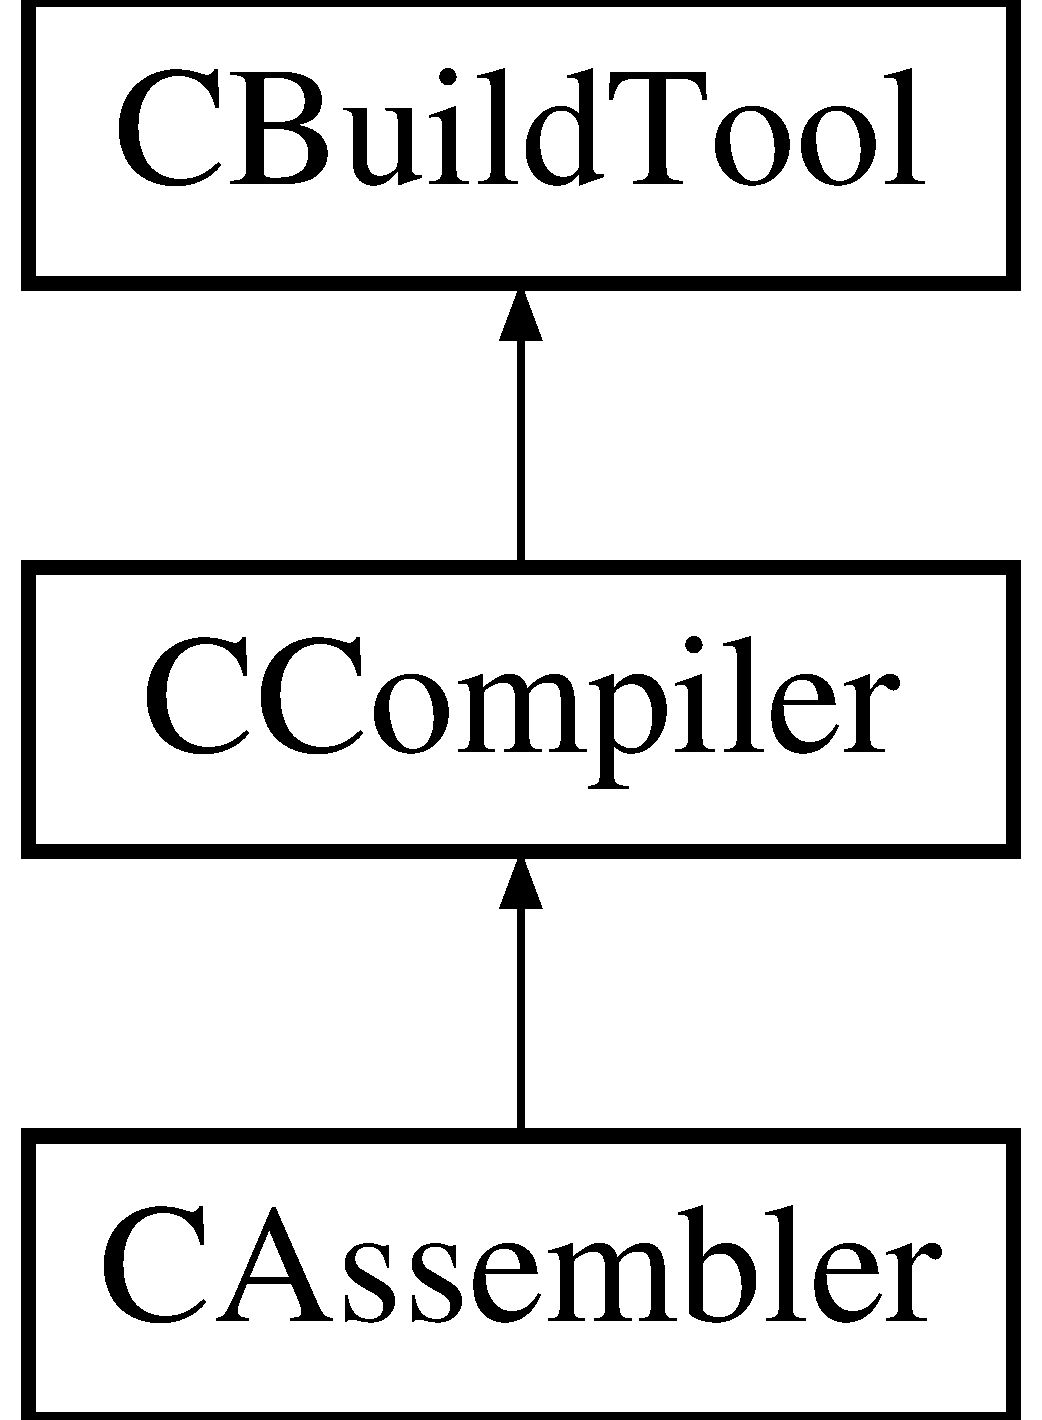
\includegraphics[height=3.000000cm]{d1/ddf/classCAssembler}
\end{center}
\end{figure}
\subsection*{Public Member Functions}
\begin{DoxyCompactItemize}
\item 
virtual \hyperlink{classCAssembler}{C\-Assembler} $\ast$ \hyperlink{classCAssembler_abc4ab373b93fc0980c204764afa73306}{Create\-Instance} (void)
\item 
\hyperlink{classCAssembler_a70fd8e0ff8470124a37474235a7e52bf}{C\-Assembler} (void)
\item 
\hyperlink{classCAssembler_a5e08b02af7a5bb5fbc35d3f1bbd9cca1}{C\-Assembler} (const \hyperlink{classCAssembler}{C\-Assembler} \&Assembler)
\item 
virtual \hyperlink{classCAssembler_a67f5ecec0343372cb4492e31f99aa313}{$\sim$\-C\-Assembler} (void)
\end{DoxyCompactItemize}
\subsection*{Additional Inherited Members}


\subsection{Constructor \& Destructor Documentation}
\hypertarget{classCAssembler_a70fd8e0ff8470124a37474235a7e52bf}{\index{C\-Assembler@{C\-Assembler}!C\-Assembler@{C\-Assembler}}
\index{C\-Assembler@{C\-Assembler}!CAssembler@{C\-Assembler}}
\subsubsection[{C\-Assembler}]{\setlength{\rightskip}{0pt plus 5cm}C\-Assembler\-::\-C\-Assembler (
\begin{DoxyParamCaption}
\item[{void}]{}
\end{DoxyParamCaption}
)}}\label{classCAssembler_a70fd8e0ff8470124a37474235a7e52bf}
\hypertarget{classCAssembler_a5e08b02af7a5bb5fbc35d3f1bbd9cca1}{\index{C\-Assembler@{C\-Assembler}!C\-Assembler@{C\-Assembler}}
\index{C\-Assembler@{C\-Assembler}!CAssembler@{C\-Assembler}}
\subsubsection[{C\-Assembler}]{\setlength{\rightskip}{0pt plus 5cm}C\-Assembler\-::\-C\-Assembler (
\begin{DoxyParamCaption}
\item[{const {\bf C\-Assembler} \&}]{Assembler}
\end{DoxyParamCaption}
)}}\label{classCAssembler_a5e08b02af7a5bb5fbc35d3f1bbd9cca1}
\hypertarget{classCAssembler_a67f5ecec0343372cb4492e31f99aa313}{\index{C\-Assembler@{C\-Assembler}!$\sim$\-C\-Assembler@{$\sim$\-C\-Assembler}}
\index{$\sim$\-C\-Assembler@{$\sim$\-C\-Assembler}!CAssembler@{C\-Assembler}}
\subsubsection[{$\sim$\-C\-Assembler}]{\setlength{\rightskip}{0pt plus 5cm}C\-Assembler\-::$\sim$\-C\-Assembler (
\begin{DoxyParamCaption}
\item[{void}]{}
\end{DoxyParamCaption}
)\hspace{0.3cm}{\ttfamily [virtual]}}}\label{classCAssembler_a67f5ecec0343372cb4492e31f99aa313}


\subsection{Member Function Documentation}
\hypertarget{classCAssembler_abc4ab373b93fc0980c204764afa73306}{\index{C\-Assembler@{C\-Assembler}!Create\-Instance@{Create\-Instance}}
\index{Create\-Instance@{Create\-Instance}!CAssembler@{C\-Assembler}}
\subsubsection[{Create\-Instance}]{\setlength{\rightskip}{0pt plus 5cm}{\bf C\-Assembler} $\ast$ C\-Assembler\-::\-Create\-Instance (
\begin{DoxyParamCaption}
\item[{void}]{}
\end{DoxyParamCaption}
)\hspace{0.3cm}{\ttfamily [virtual]}}}\label{classCAssembler_abc4ab373b93fc0980c204764afa73306}


Reimplemented from \hyperlink{classCCompiler_a3d4aaaf69e1ba6070c729fd042d90012}{C\-Compiler}.



The documentation for this class was generated from the following files\-:\begin{DoxyCompactItemize}
\item 
src/\hyperlink{buildtools_8h}{buildtools.\-h}\item 
src/\hyperlink{buildtools_8cpp}{buildtools.\-cpp}\end{DoxyCompactItemize}

\hypertarget{classCBooleanVariable}{\section{C\-Boolean\-Variable Class Reference}
\label{classCBooleanVariable}\index{C\-Boolean\-Variable@{C\-Boolean\-Variable}}
}


{\ttfamily \#include $<$stlvariables.\-h$>$}

Inheritance diagram for C\-Boolean\-Variable\-:\begin{figure}[H]
\begin{center}
\leavevmode
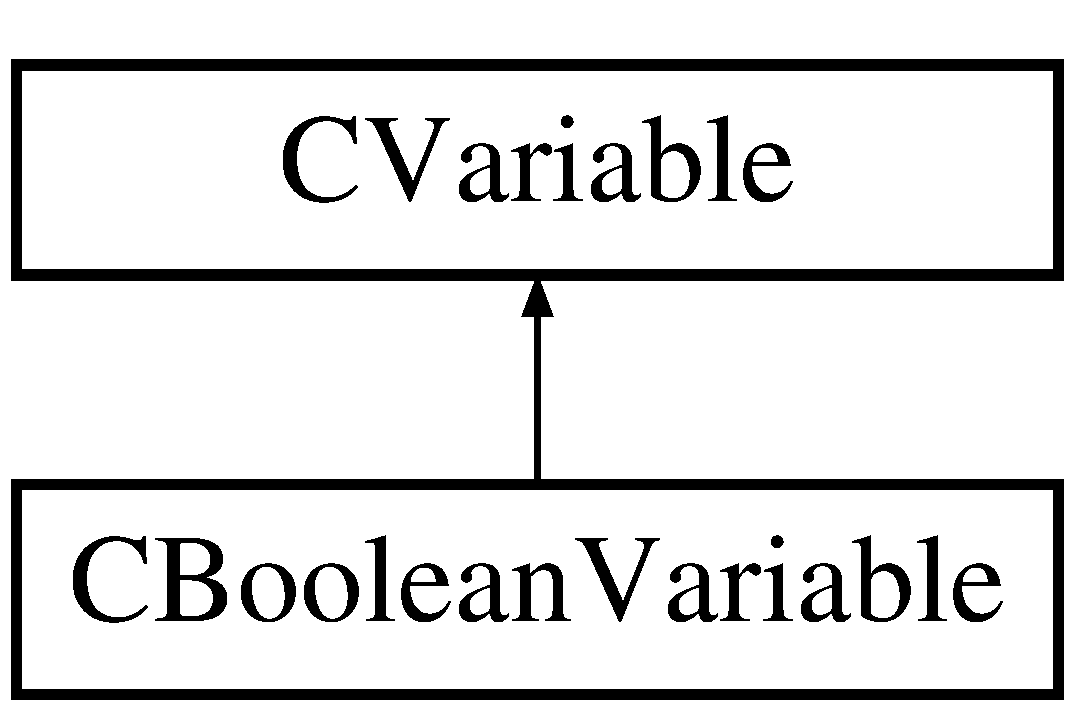
\includegraphics[height=2.000000cm]{d3/de8/classCBooleanVariable}
\end{center}
\end{figure}
\subsection*{Public Member Functions}
\begin{DoxyCompactItemize}
\item 
virtual int \hyperlink{classCBooleanVariable_ad1e47ce945773e7059e53a620bc24351}{Get\-Type} (void) const 
\item 
virtual \hyperlink{classCString}{C\-String} \hyperlink{classCBooleanVariable_a72ecdaf420fc78941793d4cab2ed6bed}{Get\-Type\-Name} (void) const 
\item 
virtual double \hyperlink{classCBooleanVariable_ac59dc433ef72caeffa5b81ea66d90da5}{Get\-Float} (void) const 
\item 
virtual void \hyperlink{classCBooleanVariable_a8cb0cdb3b3f8dad9e1b04c88f33367d8}{Set\-Float} (const double Value)
\item 
virtual int \hyperlink{classCBooleanVariable_a35aee52260e1acbdf9639845409b6614}{Get\-Integer} (void) const 
\item 
virtual void \hyperlink{classCBooleanVariable_a56fb37e55eddd15047842f92c4fa501d}{Set\-Integer} (const int Value)
\item 
virtual bool \hyperlink{classCBooleanVariable_aede73252b492061d90e44003f6d944f1}{Get\-Boolean} (void) const 
\item 
virtual void \hyperlink{classCBooleanVariable_a15c508649f6e342640fc008cf43f22db}{Set\-Boolean} (const bool Value)
\item 
virtual \hyperlink{classCString}{C\-String} \hyperlink{classCBooleanVariable_a16efdf664ecbd74b3bc0d518d76585d6}{Get\-String} (void) const 
\item 
virtual void \hyperlink{classCBooleanVariable_aa7362a06640bf84322444e85094ad5ee}{Set\-String} (const \hyperlink{classCString}{C\-String} \&Value)
\item 
virtual char \hyperlink{classCBooleanVariable_a0e9acd743061a594920afabfd6ab6eb6}{Get\-Char} (void) const 
\item 
virtual void \hyperlink{classCBooleanVariable_af22fb31d331ce7d3283abe39c92b1ec1}{Set\-Char} (const char Value)
\item 
bool \hyperlink{classCBooleanVariable_a63cba7ebfbe8782ca83860ff5d03f08b}{operator=} (const \hyperlink{classCBooleanVariable}{C\-Boolean\-Variable} \&Variable)
\item 
\hyperlink{classCBooleanVariable}{C\-Boolean\-Variable} \& \hyperlink{classCBooleanVariable_a13ff940a5bf564ba648858ca0895d159}{operator=} (const double Value)
\item 
\hyperlink{classCBooleanVariable}{C\-Boolean\-Variable} \& \hyperlink{classCBooleanVariable_a98ff04b706738d9b760ed682ad01ead7}{operator=} (const int Value)
\item 
\hyperlink{classCBooleanVariable}{C\-Boolean\-Variable} \& \hyperlink{classCBooleanVariable_a11c8041248147e45d551c35ac87347e1}{operator=} (const bool Value)
\item 
\hyperlink{classCBooleanVariable}{C\-Boolean\-Variable} \& \hyperlink{classCBooleanVariable_a824c2327fe446efe041e1688aea7b4af}{operator=} (const \hyperlink{classCString}{C\-String} \&Value)
\item 
\hyperlink{classCBooleanVariable}{C\-Boolean\-Variable} \& \hyperlink{classCBooleanVariable_a05ab1b8170a3515404218bac2cfd1b97}{operator=} (const char Value)
\item 
\hyperlink{classCBooleanVariable_a25df44d1ba844180a628b450cc2848b6}{C\-Boolean\-Variable} (const \hyperlink{classCString}{C\-String} \&Name, const bool Value=false)
\item 
virtual \hyperlink{classCBooleanVariable_ad8ce4d60d3467385816768bc0323badb}{$\sim$\-C\-Boolean\-Variable} (void)
\end{DoxyCompactItemize}
\subsection*{Protected Attributes}
\begin{DoxyCompactItemize}
\item 
bool \hyperlink{classCBooleanVariable_a768531fa3007ef064cd33bdd68a4c5b5}{m\-\_\-\-Value}
\end{DoxyCompactItemize}


\subsection{Constructor \& Destructor Documentation}
\hypertarget{classCBooleanVariable_a25df44d1ba844180a628b450cc2848b6}{\index{C\-Boolean\-Variable@{C\-Boolean\-Variable}!C\-Boolean\-Variable@{C\-Boolean\-Variable}}
\index{C\-Boolean\-Variable@{C\-Boolean\-Variable}!CBooleanVariable@{C\-Boolean\-Variable}}
\subsubsection[{C\-Boolean\-Variable}]{\setlength{\rightskip}{0pt plus 5cm}C\-Boolean\-Variable\-::\-C\-Boolean\-Variable (
\begin{DoxyParamCaption}
\item[{const {\bf C\-String} \&}]{Name, }
\item[{const bool}]{Value = {\ttfamily false}}
\end{DoxyParamCaption}
)}}\label{classCBooleanVariable_a25df44d1ba844180a628b450cc2848b6}
\hypertarget{classCBooleanVariable_ad8ce4d60d3467385816768bc0323badb}{\index{C\-Boolean\-Variable@{C\-Boolean\-Variable}!$\sim$\-C\-Boolean\-Variable@{$\sim$\-C\-Boolean\-Variable}}
\index{$\sim$\-C\-Boolean\-Variable@{$\sim$\-C\-Boolean\-Variable}!CBooleanVariable@{C\-Boolean\-Variable}}
\subsubsection[{$\sim$\-C\-Boolean\-Variable}]{\setlength{\rightskip}{0pt plus 5cm}virtual C\-Boolean\-Variable\-::$\sim$\-C\-Boolean\-Variable (
\begin{DoxyParamCaption}
\item[{void}]{}
\end{DoxyParamCaption}
)\hspace{0.3cm}{\ttfamily [inline]}, {\ttfamily [virtual]}}}\label{classCBooleanVariable_ad8ce4d60d3467385816768bc0323badb}


\subsection{Member Function Documentation}
\hypertarget{classCBooleanVariable_aede73252b492061d90e44003f6d944f1}{\index{C\-Boolean\-Variable@{C\-Boolean\-Variable}!Get\-Boolean@{Get\-Boolean}}
\index{Get\-Boolean@{Get\-Boolean}!CBooleanVariable@{C\-Boolean\-Variable}}
\subsubsection[{Get\-Boolean}]{\setlength{\rightskip}{0pt plus 5cm}bool C\-Boolean\-Variable\-::\-Get\-Boolean (
\begin{DoxyParamCaption}
\item[{void}]{}
\end{DoxyParamCaption}
) const\hspace{0.3cm}{\ttfamily [virtual]}}}\label{classCBooleanVariable_aede73252b492061d90e44003f6d944f1}


Reimplemented from \hyperlink{classCVariable_a874156d6b1a3a44f799c32a2455c7f49}{C\-Variable}.

\hypertarget{classCBooleanVariable_a0e9acd743061a594920afabfd6ab6eb6}{\index{C\-Boolean\-Variable@{C\-Boolean\-Variable}!Get\-Char@{Get\-Char}}
\index{Get\-Char@{Get\-Char}!CBooleanVariable@{C\-Boolean\-Variable}}
\subsubsection[{Get\-Char}]{\setlength{\rightskip}{0pt plus 5cm}char C\-Boolean\-Variable\-::\-Get\-Char (
\begin{DoxyParamCaption}
\item[{void}]{}
\end{DoxyParamCaption}
) const\hspace{0.3cm}{\ttfamily [virtual]}}}\label{classCBooleanVariable_a0e9acd743061a594920afabfd6ab6eb6}


Reimplemented from \hyperlink{classCVariable_a6635a8fd2441dcb83a39d10a78187dac}{C\-Variable}.

\hypertarget{classCBooleanVariable_ac59dc433ef72caeffa5b81ea66d90da5}{\index{C\-Boolean\-Variable@{C\-Boolean\-Variable}!Get\-Float@{Get\-Float}}
\index{Get\-Float@{Get\-Float}!CBooleanVariable@{C\-Boolean\-Variable}}
\subsubsection[{Get\-Float}]{\setlength{\rightskip}{0pt plus 5cm}double C\-Boolean\-Variable\-::\-Get\-Float (
\begin{DoxyParamCaption}
\item[{void}]{}
\end{DoxyParamCaption}
) const\hspace{0.3cm}{\ttfamily [virtual]}}}\label{classCBooleanVariable_ac59dc433ef72caeffa5b81ea66d90da5}


Reimplemented from \hyperlink{classCVariable_ac475ad87ffbfaeeb2d4d9c2986b0d575}{C\-Variable}.

\hypertarget{classCBooleanVariable_a35aee52260e1acbdf9639845409b6614}{\index{C\-Boolean\-Variable@{C\-Boolean\-Variable}!Get\-Integer@{Get\-Integer}}
\index{Get\-Integer@{Get\-Integer}!CBooleanVariable@{C\-Boolean\-Variable}}
\subsubsection[{Get\-Integer}]{\setlength{\rightskip}{0pt plus 5cm}int C\-Boolean\-Variable\-::\-Get\-Integer (
\begin{DoxyParamCaption}
\item[{void}]{}
\end{DoxyParamCaption}
) const\hspace{0.3cm}{\ttfamily [virtual]}}}\label{classCBooleanVariable_a35aee52260e1acbdf9639845409b6614}


Reimplemented from \hyperlink{classCVariable_adb0db49f4a55f3e1b5322f6ce26e4ebc}{C\-Variable}.

\hypertarget{classCBooleanVariable_a16efdf664ecbd74b3bc0d518d76585d6}{\index{C\-Boolean\-Variable@{C\-Boolean\-Variable}!Get\-String@{Get\-String}}
\index{Get\-String@{Get\-String}!CBooleanVariable@{C\-Boolean\-Variable}}
\subsubsection[{Get\-String}]{\setlength{\rightskip}{0pt plus 5cm}{\bf C\-String} C\-Boolean\-Variable\-::\-Get\-String (
\begin{DoxyParamCaption}
\item[{void}]{}
\end{DoxyParamCaption}
) const\hspace{0.3cm}{\ttfamily [virtual]}}}\label{classCBooleanVariable_a16efdf664ecbd74b3bc0d518d76585d6}


Reimplemented from \hyperlink{classCVariable_aefa25c880c0042ffc29889475d329004}{C\-Variable}.

\hypertarget{classCBooleanVariable_ad1e47ce945773e7059e53a620bc24351}{\index{C\-Boolean\-Variable@{C\-Boolean\-Variable}!Get\-Type@{Get\-Type}}
\index{Get\-Type@{Get\-Type}!CBooleanVariable@{C\-Boolean\-Variable}}
\subsubsection[{Get\-Type}]{\setlength{\rightskip}{0pt plus 5cm}int C\-Boolean\-Variable\-::\-Get\-Type (
\begin{DoxyParamCaption}
\item[{void}]{}
\end{DoxyParamCaption}
) const\hspace{0.3cm}{\ttfamily [virtual]}}}\label{classCBooleanVariable_ad1e47ce945773e7059e53a620bc24351}


Reimplemented from \hyperlink{classCVariable_acdf7301ad2f5c7fa33770c028211c0bc}{C\-Variable}.

\hypertarget{classCBooleanVariable_a72ecdaf420fc78941793d4cab2ed6bed}{\index{C\-Boolean\-Variable@{C\-Boolean\-Variable}!Get\-Type\-Name@{Get\-Type\-Name}}
\index{Get\-Type\-Name@{Get\-Type\-Name}!CBooleanVariable@{C\-Boolean\-Variable}}
\subsubsection[{Get\-Type\-Name}]{\setlength{\rightskip}{0pt plus 5cm}{\bf C\-String} C\-Boolean\-Variable\-::\-Get\-Type\-Name (
\begin{DoxyParamCaption}
\item[{void}]{}
\end{DoxyParamCaption}
) const\hspace{0.3cm}{\ttfamily [virtual]}}}\label{classCBooleanVariable_a72ecdaf420fc78941793d4cab2ed6bed}


Reimplemented from \hyperlink{classCVariable_ad8a23d1501917cbfb1eee1473a7a2122}{C\-Variable}.

\hypertarget{classCBooleanVariable_a63cba7ebfbe8782ca83860ff5d03f08b}{\index{C\-Boolean\-Variable@{C\-Boolean\-Variable}!operator=@{operator=}}
\index{operator=@{operator=}!CBooleanVariable@{C\-Boolean\-Variable}}
\subsubsection[{operator=}]{\setlength{\rightskip}{0pt plus 5cm}bool C\-Boolean\-Variable\-::operator= (
\begin{DoxyParamCaption}
\item[{const {\bf C\-Boolean\-Variable} \&}]{Variable}
\end{DoxyParamCaption}
)}}\label{classCBooleanVariable_a63cba7ebfbe8782ca83860ff5d03f08b}
\hypertarget{classCBooleanVariable_a13ff940a5bf564ba648858ca0895d159}{\index{C\-Boolean\-Variable@{C\-Boolean\-Variable}!operator=@{operator=}}
\index{operator=@{operator=}!CBooleanVariable@{C\-Boolean\-Variable}}
\subsubsection[{operator=}]{\setlength{\rightskip}{0pt plus 5cm}{\bf C\-Boolean\-Variable} \& C\-Boolean\-Variable\-::operator= (
\begin{DoxyParamCaption}
\item[{const double}]{Value}
\end{DoxyParamCaption}
)}}\label{classCBooleanVariable_a13ff940a5bf564ba648858ca0895d159}
\hypertarget{classCBooleanVariable_a98ff04b706738d9b760ed682ad01ead7}{\index{C\-Boolean\-Variable@{C\-Boolean\-Variable}!operator=@{operator=}}
\index{operator=@{operator=}!CBooleanVariable@{C\-Boolean\-Variable}}
\subsubsection[{operator=}]{\setlength{\rightskip}{0pt plus 5cm}{\bf C\-Boolean\-Variable} \& C\-Boolean\-Variable\-::operator= (
\begin{DoxyParamCaption}
\item[{const int}]{Value}
\end{DoxyParamCaption}
)}}\label{classCBooleanVariable_a98ff04b706738d9b760ed682ad01ead7}
\hypertarget{classCBooleanVariable_a11c8041248147e45d551c35ac87347e1}{\index{C\-Boolean\-Variable@{C\-Boolean\-Variable}!operator=@{operator=}}
\index{operator=@{operator=}!CBooleanVariable@{C\-Boolean\-Variable}}
\subsubsection[{operator=}]{\setlength{\rightskip}{0pt plus 5cm}{\bf C\-Boolean\-Variable} \& C\-Boolean\-Variable\-::operator= (
\begin{DoxyParamCaption}
\item[{const bool}]{Value}
\end{DoxyParamCaption}
)}}\label{classCBooleanVariable_a11c8041248147e45d551c35ac87347e1}
\hypertarget{classCBooleanVariable_a824c2327fe446efe041e1688aea7b4af}{\index{C\-Boolean\-Variable@{C\-Boolean\-Variable}!operator=@{operator=}}
\index{operator=@{operator=}!CBooleanVariable@{C\-Boolean\-Variable}}
\subsubsection[{operator=}]{\setlength{\rightskip}{0pt plus 5cm}{\bf C\-Boolean\-Variable} \& C\-Boolean\-Variable\-::operator= (
\begin{DoxyParamCaption}
\item[{const {\bf C\-String} \&}]{Value}
\end{DoxyParamCaption}
)}}\label{classCBooleanVariable_a824c2327fe446efe041e1688aea7b4af}
\hypertarget{classCBooleanVariable_a05ab1b8170a3515404218bac2cfd1b97}{\index{C\-Boolean\-Variable@{C\-Boolean\-Variable}!operator=@{operator=}}
\index{operator=@{operator=}!CBooleanVariable@{C\-Boolean\-Variable}}
\subsubsection[{operator=}]{\setlength{\rightskip}{0pt plus 5cm}{\bf C\-Boolean\-Variable} \& C\-Boolean\-Variable\-::operator= (
\begin{DoxyParamCaption}
\item[{const char}]{Value}
\end{DoxyParamCaption}
)}}\label{classCBooleanVariable_a05ab1b8170a3515404218bac2cfd1b97}
\hypertarget{classCBooleanVariable_a15c508649f6e342640fc008cf43f22db}{\index{C\-Boolean\-Variable@{C\-Boolean\-Variable}!Set\-Boolean@{Set\-Boolean}}
\index{Set\-Boolean@{Set\-Boolean}!CBooleanVariable@{C\-Boolean\-Variable}}
\subsubsection[{Set\-Boolean}]{\setlength{\rightskip}{0pt plus 5cm}void C\-Boolean\-Variable\-::\-Set\-Boolean (
\begin{DoxyParamCaption}
\item[{const bool}]{Value}
\end{DoxyParamCaption}
)\hspace{0.3cm}{\ttfamily [virtual]}}}\label{classCBooleanVariable_a15c508649f6e342640fc008cf43f22db}


Reimplemented from \hyperlink{classCVariable_a5c8d2cb9ae53c01dc1ec7e45f8903126}{C\-Variable}.

\hypertarget{classCBooleanVariable_af22fb31d331ce7d3283abe39c92b1ec1}{\index{C\-Boolean\-Variable@{C\-Boolean\-Variable}!Set\-Char@{Set\-Char}}
\index{Set\-Char@{Set\-Char}!CBooleanVariable@{C\-Boolean\-Variable}}
\subsubsection[{Set\-Char}]{\setlength{\rightskip}{0pt plus 5cm}void C\-Boolean\-Variable\-::\-Set\-Char (
\begin{DoxyParamCaption}
\item[{const char}]{Value}
\end{DoxyParamCaption}
)\hspace{0.3cm}{\ttfamily [virtual]}}}\label{classCBooleanVariable_af22fb31d331ce7d3283abe39c92b1ec1}


Reimplemented from \hyperlink{classCVariable_a10a96343a4a2437b02b7105adf87a64c}{C\-Variable}.

\hypertarget{classCBooleanVariable_a8cb0cdb3b3f8dad9e1b04c88f33367d8}{\index{C\-Boolean\-Variable@{C\-Boolean\-Variable}!Set\-Float@{Set\-Float}}
\index{Set\-Float@{Set\-Float}!CBooleanVariable@{C\-Boolean\-Variable}}
\subsubsection[{Set\-Float}]{\setlength{\rightskip}{0pt plus 5cm}void C\-Boolean\-Variable\-::\-Set\-Float (
\begin{DoxyParamCaption}
\item[{const double}]{Value}
\end{DoxyParamCaption}
)\hspace{0.3cm}{\ttfamily [virtual]}}}\label{classCBooleanVariable_a8cb0cdb3b3f8dad9e1b04c88f33367d8}


Reimplemented from \hyperlink{classCVariable_ae352cd2c25541c1137b0f12926d09995}{C\-Variable}.

\hypertarget{classCBooleanVariable_a56fb37e55eddd15047842f92c4fa501d}{\index{C\-Boolean\-Variable@{C\-Boolean\-Variable}!Set\-Integer@{Set\-Integer}}
\index{Set\-Integer@{Set\-Integer}!CBooleanVariable@{C\-Boolean\-Variable}}
\subsubsection[{Set\-Integer}]{\setlength{\rightskip}{0pt plus 5cm}void C\-Boolean\-Variable\-::\-Set\-Integer (
\begin{DoxyParamCaption}
\item[{const int}]{Value}
\end{DoxyParamCaption}
)\hspace{0.3cm}{\ttfamily [virtual]}}}\label{classCBooleanVariable_a56fb37e55eddd15047842f92c4fa501d}


Reimplemented from \hyperlink{classCVariable_ab97d7164ed35ca67d4bacaebbc7f6fe6}{C\-Variable}.

\hypertarget{classCBooleanVariable_aa7362a06640bf84322444e85094ad5ee}{\index{C\-Boolean\-Variable@{C\-Boolean\-Variable}!Set\-String@{Set\-String}}
\index{Set\-String@{Set\-String}!CBooleanVariable@{C\-Boolean\-Variable}}
\subsubsection[{Set\-String}]{\setlength{\rightskip}{0pt plus 5cm}void C\-Boolean\-Variable\-::\-Set\-String (
\begin{DoxyParamCaption}
\item[{const {\bf C\-String} \&}]{Value}
\end{DoxyParamCaption}
)\hspace{0.3cm}{\ttfamily [virtual]}}}\label{classCBooleanVariable_aa7362a06640bf84322444e85094ad5ee}


Reimplemented from \hyperlink{classCVariable_a7c536a5709d8df5d9d75013370288c79}{C\-Variable}.



\subsection{Member Data Documentation}
\hypertarget{classCBooleanVariable_a768531fa3007ef064cd33bdd68a4c5b5}{\index{C\-Boolean\-Variable@{C\-Boolean\-Variable}!m\-\_\-\-Value@{m\-\_\-\-Value}}
\index{m\-\_\-\-Value@{m\-\_\-\-Value}!CBooleanVariable@{C\-Boolean\-Variable}}
\subsubsection[{m\-\_\-\-Value}]{\setlength{\rightskip}{0pt plus 5cm}bool C\-Boolean\-Variable\-::m\-\_\-\-Value\hspace{0.3cm}{\ttfamily [protected]}}}\label{classCBooleanVariable_a768531fa3007ef064cd33bdd68a4c5b5}


The documentation for this class was generated from the following files\-:\begin{DoxyCompactItemize}
\item 
lib/\hyperlink{stlvariables_8h}{stlvariables.\-h}\item 
lib/\hyperlink{stlvariables_8cpp}{stlvariables.\-cpp}\end{DoxyCompactItemize}

\hypertarget{classCBorlandConsoleExecutableLinker}{\section{C\-Borland\-Console\-Executable\-Linker Class Reference}
\label{classCBorlandConsoleExecutableLinker}\index{C\-Borland\-Console\-Executable\-Linker@{C\-Borland\-Console\-Executable\-Linker}}
}


{\ttfamily \#include $<$buildtools.\-h$>$}

Inheritance diagram for C\-Borland\-Console\-Executable\-Linker\-:\begin{figure}[H]
\begin{center}
\leavevmode
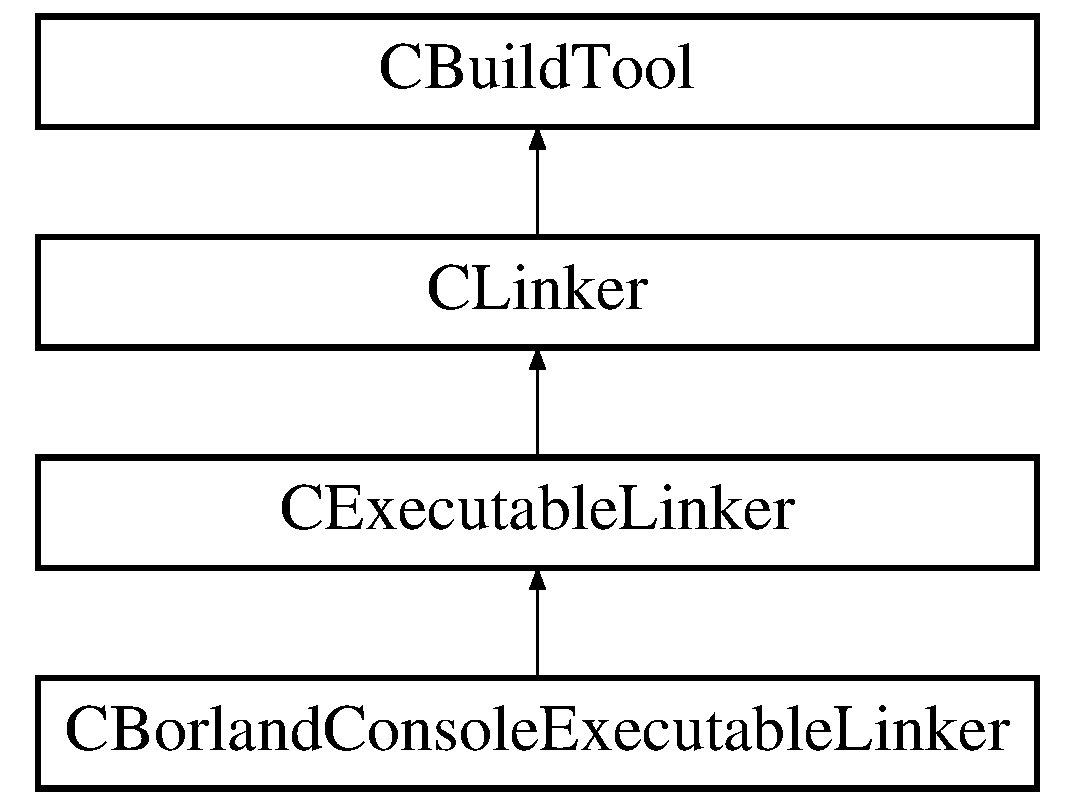
\includegraphics[height=4.000000cm]{d8/dbd/classCBorlandConsoleExecutableLinker}
\end{center}
\end{figure}
\subsection*{Public Member Functions}
\begin{DoxyCompactItemize}
\item 
virtual \\*
\hyperlink{classCBorlandConsoleExecutableLinker}{C\-Borland\-Console\-Executable\-Linker} $\ast$ \hyperlink{classCBorlandConsoleExecutableLinker_a1aba394784a724a2b59c021b732484f8}{Create\-Instance} (void)
\item 
virtual void \hyperlink{classCBorlandConsoleExecutableLinker_a0b31e3b17b2c03a4d6d6ada4fe8b48e0}{Reset} (const \hyperlink{classCPlatform_a2fb735c63c53052f79629e338bb0f535}{C\-Platform\-::\-O\-S\-\_\-\-Type} O\-S)
\item 
virtual bool \hyperlink{classCBorlandConsoleExecutableLinker_a3f6d2df3415c6ee0cec057b481378b45}{Supports} (const \hyperlink{classCPlatform_a2fb735c63c53052f79629e338bb0f535}{C\-Platform\-::\-O\-S\-\_\-\-Type} O\-S)
\item 
\hyperlink{classCBorlandConsoleExecutableLinker_a95ce52cd5ad5703509d75bb179b6e89e}{C\-Borland\-Console\-Executable\-Linker} (void)
\end{DoxyCompactItemize}
\subsection*{Additional Inherited Members}


\subsection{Constructor \& Destructor Documentation}
\hypertarget{classCBorlandConsoleExecutableLinker_a95ce52cd5ad5703509d75bb179b6e89e}{\index{C\-Borland\-Console\-Executable\-Linker@{C\-Borland\-Console\-Executable\-Linker}!C\-Borland\-Console\-Executable\-Linker@{C\-Borland\-Console\-Executable\-Linker}}
\index{C\-Borland\-Console\-Executable\-Linker@{C\-Borland\-Console\-Executable\-Linker}!CBorlandConsoleExecutableLinker@{C\-Borland\-Console\-Executable\-Linker}}
\subsubsection[{C\-Borland\-Console\-Executable\-Linker}]{\setlength{\rightskip}{0pt plus 5cm}C\-Borland\-Console\-Executable\-Linker\-::\-C\-Borland\-Console\-Executable\-Linker (
\begin{DoxyParamCaption}
\item[{void}]{}
\end{DoxyParamCaption}
)}}\label{classCBorlandConsoleExecutableLinker_a95ce52cd5ad5703509d75bb179b6e89e}


\subsection{Member Function Documentation}
\hypertarget{classCBorlandConsoleExecutableLinker_a1aba394784a724a2b59c021b732484f8}{\index{C\-Borland\-Console\-Executable\-Linker@{C\-Borland\-Console\-Executable\-Linker}!Create\-Instance@{Create\-Instance}}
\index{Create\-Instance@{Create\-Instance}!CBorlandConsoleExecutableLinker@{C\-Borland\-Console\-Executable\-Linker}}
\subsubsection[{Create\-Instance}]{\setlength{\rightskip}{0pt plus 5cm}{\bf C\-Borland\-Console\-Executable\-Linker} $\ast$ C\-Borland\-Console\-Executable\-Linker\-::\-Create\-Instance (
\begin{DoxyParamCaption}
\item[{void}]{}
\end{DoxyParamCaption}
)\hspace{0.3cm}{\ttfamily [virtual]}}}\label{classCBorlandConsoleExecutableLinker_a1aba394784a724a2b59c021b732484f8}


Reimplemented from \hyperlink{classCExecutableLinker_a457b823b737b0a78285d5ede77df827c}{C\-Executable\-Linker}.

\hypertarget{classCBorlandConsoleExecutableLinker_a0b31e3b17b2c03a4d6d6ada4fe8b48e0}{\index{C\-Borland\-Console\-Executable\-Linker@{C\-Borland\-Console\-Executable\-Linker}!Reset@{Reset}}
\index{Reset@{Reset}!CBorlandConsoleExecutableLinker@{C\-Borland\-Console\-Executable\-Linker}}
\subsubsection[{Reset}]{\setlength{\rightskip}{0pt plus 5cm}void C\-Borland\-Console\-Executable\-Linker\-::\-Reset (
\begin{DoxyParamCaption}
\item[{const {\bf C\-Platform\-::\-O\-S\-\_\-\-Type}}]{O\-S}
\end{DoxyParamCaption}
)\hspace{0.3cm}{\ttfamily [virtual]}}}\label{classCBorlandConsoleExecutableLinker_a0b31e3b17b2c03a4d6d6ada4fe8b48e0}


Reimplemented from \hyperlink{classCBuildTool_abea21a0e61ab2177effdff5aaa169585}{C\-Build\-Tool}.

\hypertarget{classCBorlandConsoleExecutableLinker_a3f6d2df3415c6ee0cec057b481378b45}{\index{C\-Borland\-Console\-Executable\-Linker@{C\-Borland\-Console\-Executable\-Linker}!Supports@{Supports}}
\index{Supports@{Supports}!CBorlandConsoleExecutableLinker@{C\-Borland\-Console\-Executable\-Linker}}
\subsubsection[{Supports}]{\setlength{\rightskip}{0pt plus 5cm}bool C\-Borland\-Console\-Executable\-Linker\-::\-Supports (
\begin{DoxyParamCaption}
\item[{const {\bf C\-Platform\-::\-O\-S\-\_\-\-Type}}]{O\-S}
\end{DoxyParamCaption}
)\hspace{0.3cm}{\ttfamily [virtual]}}}\label{classCBorlandConsoleExecutableLinker_a3f6d2df3415c6ee0cec057b481378b45}


Reimplemented from \hyperlink{classCBuildTool_ad07fcd46ccc841bc131d65505e5343c1}{C\-Build\-Tool}.



The documentation for this class was generated from the following files\-:\begin{DoxyCompactItemize}
\item 
src/\hyperlink{buildtools_8h}{buildtools.\-h}\item 
src/\hyperlink{buildtools_8cpp}{buildtools.\-cpp}\end{DoxyCompactItemize}

\hypertarget{classCBorlandCppCompiler}{\section{C\-Borland\-Cpp\-Compiler Class Reference}
\label{classCBorlandCppCompiler}\index{C\-Borland\-Cpp\-Compiler@{C\-Borland\-Cpp\-Compiler}}
}


{\ttfamily \#include $<$buildtools.\-h$>$}

Inheritance diagram for C\-Borland\-Cpp\-Compiler\-:\begin{figure}[H]
\begin{center}
\leavevmode
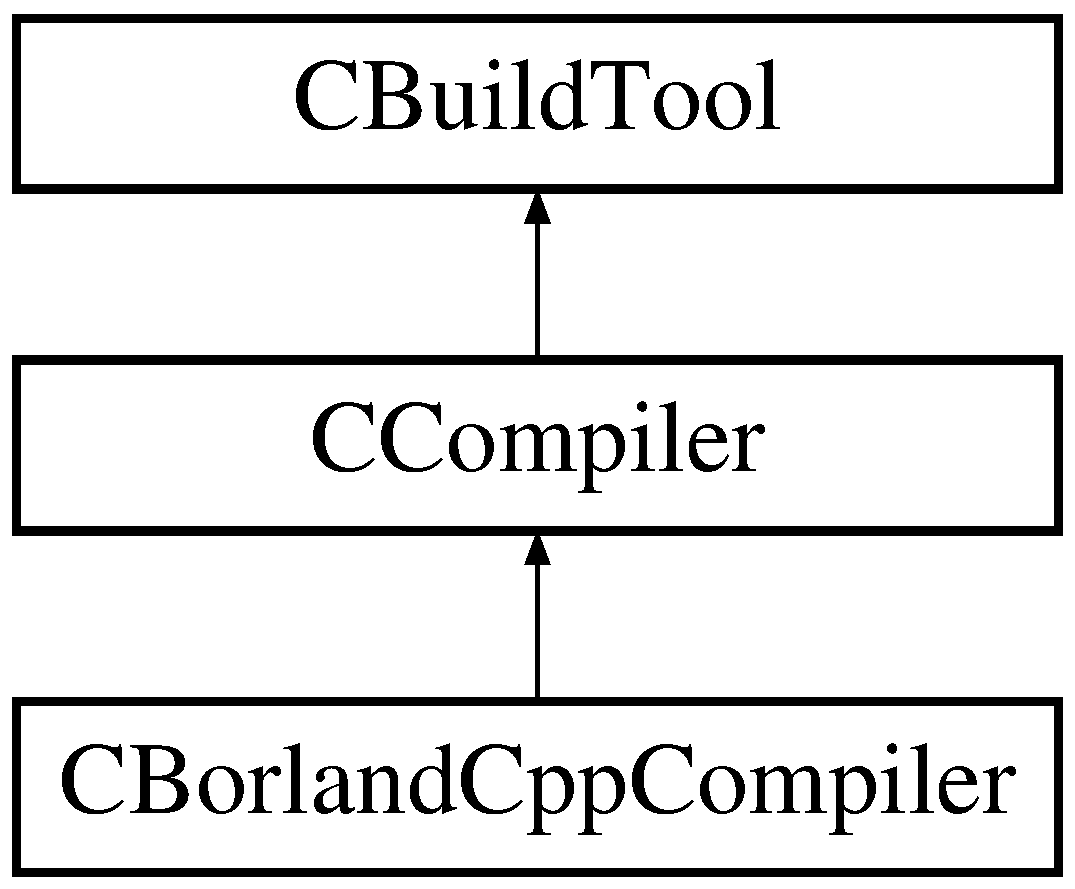
\includegraphics[height=3.000000cm]{da/dd2/classCBorlandCppCompiler}
\end{center}
\end{figure}
\subsection*{Public Member Functions}
\begin{DoxyCompactItemize}
\item 
virtual \hyperlink{classCIncludeSearchFilter}{C\-Include\-Search\-Filter} $\ast$ \hyperlink{classCBorlandCppCompiler_a9619772f500bb2f06d4a07349b08d05d}{Include\-Search\-Filter} (void) const 
\item 
virtual \hyperlink{classCBorlandCppCompiler}{C\-Borland\-Cpp\-Compiler} $\ast$ \hyperlink{classCBorlandCppCompiler_a49178aa21245a1400f38c71631b7fa78}{Create\-Instance} (void)
\item 
virtual void \hyperlink{classCBorlandCppCompiler_ac329f9e685bd1a702d7545fa991be71d}{Reset} (const \hyperlink{classCPlatform_a2fb735c63c53052f79629e338bb0f535}{C\-Platform\-::\-O\-S\-\_\-\-Type} O\-S)
\item 
virtual bool \hyperlink{classCBorlandCppCompiler_a68255b1124b821456884050014e1b256}{Supports} (const \hyperlink{classCPlatform_a2fb735c63c53052f79629e338bb0f535}{C\-Platform\-::\-O\-S\-\_\-\-Type} O\-S)
\item 
\hyperlink{classCBorlandCppCompiler_aaa978e5b4d1f2f941b57838c4082d8f2}{C\-Borland\-Cpp\-Compiler} (void)
\end{DoxyCompactItemize}
\subsection*{Private Attributes}
\begin{DoxyCompactItemize}
\item 
\hyperlink{classCCppIncludeSearchFilter}{C\-Cpp\-Include\-Search\-Filter} \hyperlink{classCBorlandCppCompiler_a14852b7a3ed29696f0a187698a1c3b70}{m\-\_\-\-Include\-Search\-Filter}
\end{DoxyCompactItemize}
\subsection*{Additional Inherited Members}


\subsection{Constructor \& Destructor Documentation}
\hypertarget{classCBorlandCppCompiler_aaa978e5b4d1f2f941b57838c4082d8f2}{\index{C\-Borland\-Cpp\-Compiler@{C\-Borland\-Cpp\-Compiler}!C\-Borland\-Cpp\-Compiler@{C\-Borland\-Cpp\-Compiler}}
\index{C\-Borland\-Cpp\-Compiler@{C\-Borland\-Cpp\-Compiler}!CBorlandCppCompiler@{C\-Borland\-Cpp\-Compiler}}
\subsubsection[{C\-Borland\-Cpp\-Compiler}]{\setlength{\rightskip}{0pt plus 5cm}C\-Borland\-Cpp\-Compiler\-::\-C\-Borland\-Cpp\-Compiler (
\begin{DoxyParamCaption}
\item[{void}]{}
\end{DoxyParamCaption}
)}}\label{classCBorlandCppCompiler_aaa978e5b4d1f2f941b57838c4082d8f2}


\subsection{Member Function Documentation}
\hypertarget{classCBorlandCppCompiler_a49178aa21245a1400f38c71631b7fa78}{\index{C\-Borland\-Cpp\-Compiler@{C\-Borland\-Cpp\-Compiler}!Create\-Instance@{Create\-Instance}}
\index{Create\-Instance@{Create\-Instance}!CBorlandCppCompiler@{C\-Borland\-Cpp\-Compiler}}
\subsubsection[{Create\-Instance}]{\setlength{\rightskip}{0pt plus 5cm}{\bf C\-Borland\-Cpp\-Compiler} $\ast$ C\-Borland\-Cpp\-Compiler\-::\-Create\-Instance (
\begin{DoxyParamCaption}
\item[{void}]{}
\end{DoxyParamCaption}
)\hspace{0.3cm}{\ttfamily [virtual]}}}\label{classCBorlandCppCompiler_a49178aa21245a1400f38c71631b7fa78}


Reimplemented from \hyperlink{classCCompiler_a3d4aaaf69e1ba6070c729fd042d90012}{C\-Compiler}.

\hypertarget{classCBorlandCppCompiler_a9619772f500bb2f06d4a07349b08d05d}{\index{C\-Borland\-Cpp\-Compiler@{C\-Borland\-Cpp\-Compiler}!Include\-Search\-Filter@{Include\-Search\-Filter}}
\index{Include\-Search\-Filter@{Include\-Search\-Filter}!CBorlandCppCompiler@{C\-Borland\-Cpp\-Compiler}}
\subsubsection[{Include\-Search\-Filter}]{\setlength{\rightskip}{0pt plus 5cm}{\bf C\-Include\-Search\-Filter} $\ast$ C\-Borland\-Cpp\-Compiler\-::\-Include\-Search\-Filter (
\begin{DoxyParamCaption}
\item[{void}]{}
\end{DoxyParamCaption}
) const\hspace{0.3cm}{\ttfamily [virtual]}}}\label{classCBorlandCppCompiler_a9619772f500bb2f06d4a07349b08d05d}


Reimplemented from \hyperlink{classCCompiler_a1dc477f47e953ddd4c653f3ba85c5468}{C\-Compiler}.

\hypertarget{classCBorlandCppCompiler_ac329f9e685bd1a702d7545fa991be71d}{\index{C\-Borland\-Cpp\-Compiler@{C\-Borland\-Cpp\-Compiler}!Reset@{Reset}}
\index{Reset@{Reset}!CBorlandCppCompiler@{C\-Borland\-Cpp\-Compiler}}
\subsubsection[{Reset}]{\setlength{\rightskip}{0pt plus 5cm}void C\-Borland\-Cpp\-Compiler\-::\-Reset (
\begin{DoxyParamCaption}
\item[{const {\bf C\-Platform\-::\-O\-S\-\_\-\-Type}}]{O\-S}
\end{DoxyParamCaption}
)\hspace{0.3cm}{\ttfamily [virtual]}}}\label{classCBorlandCppCompiler_ac329f9e685bd1a702d7545fa991be71d}


Reimplemented from \hyperlink{classCBuildTool_abea21a0e61ab2177effdff5aaa169585}{C\-Build\-Tool}.

\hypertarget{classCBorlandCppCompiler_a68255b1124b821456884050014e1b256}{\index{C\-Borland\-Cpp\-Compiler@{C\-Borland\-Cpp\-Compiler}!Supports@{Supports}}
\index{Supports@{Supports}!CBorlandCppCompiler@{C\-Borland\-Cpp\-Compiler}}
\subsubsection[{Supports}]{\setlength{\rightskip}{0pt plus 5cm}bool C\-Borland\-Cpp\-Compiler\-::\-Supports (
\begin{DoxyParamCaption}
\item[{const {\bf C\-Platform\-::\-O\-S\-\_\-\-Type}}]{O\-S}
\end{DoxyParamCaption}
)\hspace{0.3cm}{\ttfamily [virtual]}}}\label{classCBorlandCppCompiler_a68255b1124b821456884050014e1b256}


Reimplemented from \hyperlink{classCBuildTool_ad07fcd46ccc841bc131d65505e5343c1}{C\-Build\-Tool}.



\subsection{Member Data Documentation}
\hypertarget{classCBorlandCppCompiler_a14852b7a3ed29696f0a187698a1c3b70}{\index{C\-Borland\-Cpp\-Compiler@{C\-Borland\-Cpp\-Compiler}!m\-\_\-\-Include\-Search\-Filter@{m\-\_\-\-Include\-Search\-Filter}}
\index{m\-\_\-\-Include\-Search\-Filter@{m\-\_\-\-Include\-Search\-Filter}!CBorlandCppCompiler@{C\-Borland\-Cpp\-Compiler}}
\subsubsection[{m\-\_\-\-Include\-Search\-Filter}]{\setlength{\rightskip}{0pt plus 5cm}{\bf C\-Cpp\-Include\-Search\-Filter} C\-Borland\-Cpp\-Compiler\-::m\-\_\-\-Include\-Search\-Filter\hspace{0.3cm}{\ttfamily [private]}}}\label{classCBorlandCppCompiler_a14852b7a3ed29696f0a187698a1c3b70}


The documentation for this class was generated from the following files\-:\begin{DoxyCompactItemize}
\item 
src/\hyperlink{buildtools_8h}{buildtools.\-h}\item 
src/\hyperlink{buildtools_8cpp}{buildtools.\-cpp}\end{DoxyCompactItemize}

\hypertarget{classCBorlandDynamicLinker}{\section{C\-Borland\-Dynamic\-Linker Class Reference}
\label{classCBorlandDynamicLinker}\index{C\-Borland\-Dynamic\-Linker@{C\-Borland\-Dynamic\-Linker}}
}


{\ttfamily \#include $<$buildtools.\-h$>$}

Inheritance diagram for C\-Borland\-Dynamic\-Linker\-:\begin{figure}[H]
\begin{center}
\leavevmode
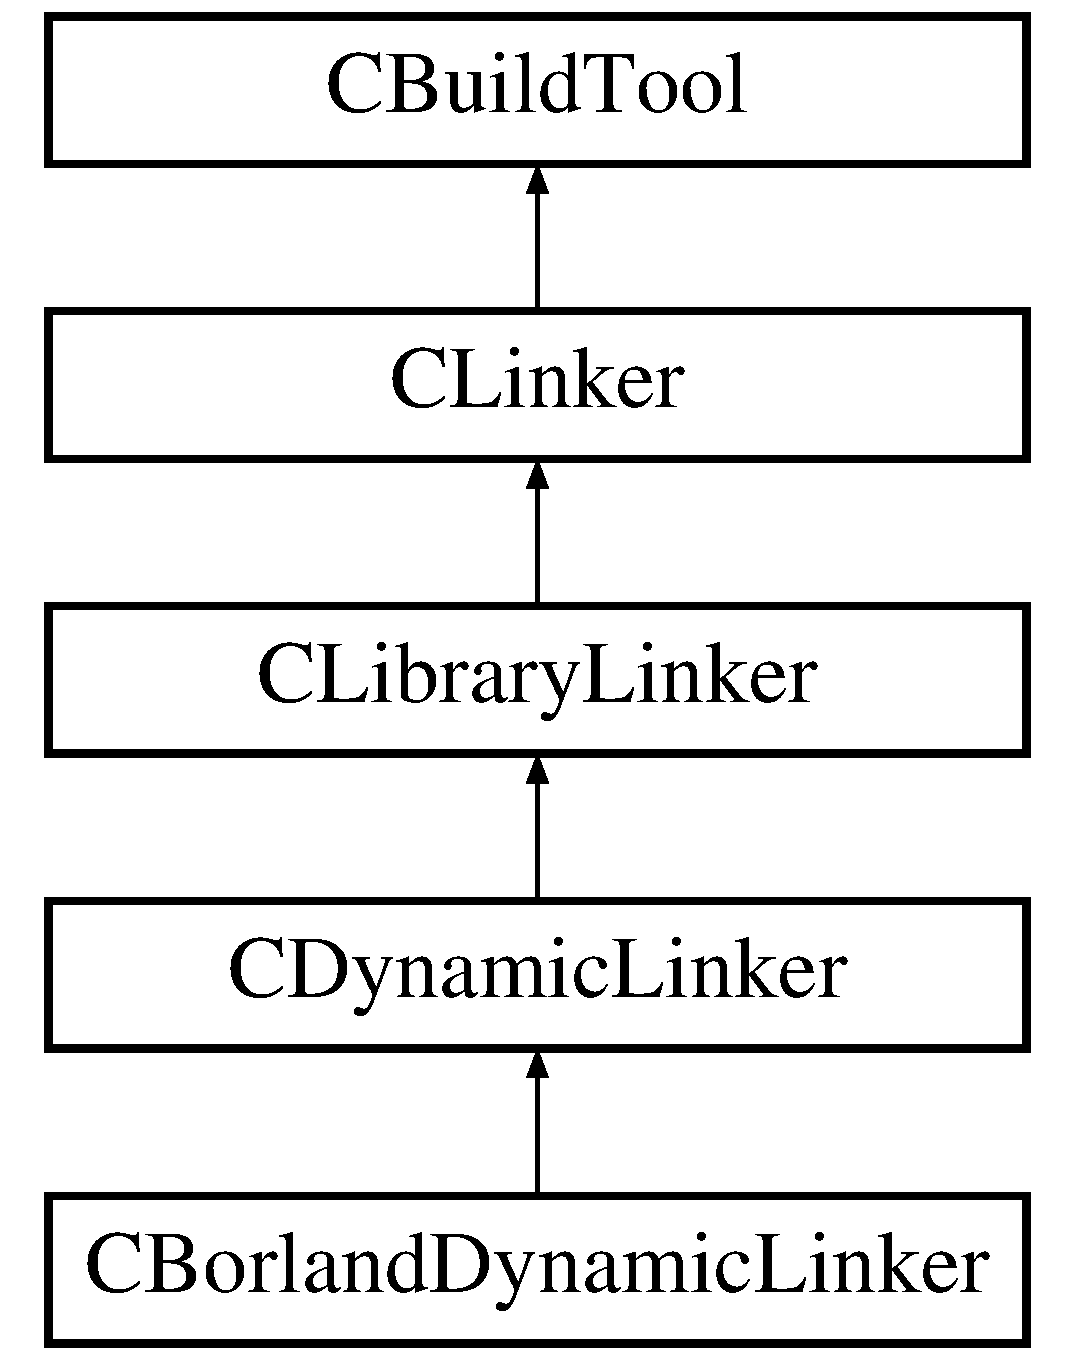
\includegraphics[height=5.000000cm]{da/d1c/classCBorlandDynamicLinker}
\end{center}
\end{figure}
\subsection*{Public Member Functions}
\begin{DoxyCompactItemize}
\item 
virtual \hyperlink{classCBorlandDynamicLinker}{C\-Borland\-Dynamic\-Linker} $\ast$ \hyperlink{classCBorlandDynamicLinker_ae76cbd521d03bd3eee2f1d5fe8836d03}{Create\-Instance} (void)
\item 
virtual void \hyperlink{classCBorlandDynamicLinker_acbf22349e7e89873dac5f55f8d9adc8b}{Reset} (const \hyperlink{classCPlatform_a2fb735c63c53052f79629e338bb0f535}{C\-Platform\-::\-O\-S\-\_\-\-Type} O\-S)
\item 
virtual bool \hyperlink{classCBorlandDynamicLinker_a78506817efc139b24fe28ebebde51942}{Supports} (const \hyperlink{classCPlatform_a2fb735c63c53052f79629e338bb0f535}{C\-Platform\-::\-O\-S\-\_\-\-Type} O\-S)
\item 
\hyperlink{classCBorlandDynamicLinker_ae16f9b25867092692e27de417640a9b1}{C\-Borland\-Dynamic\-Linker} (void)
\end{DoxyCompactItemize}
\subsection*{Additional Inherited Members}


\subsection{Constructor \& Destructor Documentation}
\hypertarget{classCBorlandDynamicLinker_ae16f9b25867092692e27de417640a9b1}{\index{C\-Borland\-Dynamic\-Linker@{C\-Borland\-Dynamic\-Linker}!C\-Borland\-Dynamic\-Linker@{C\-Borland\-Dynamic\-Linker}}
\index{C\-Borland\-Dynamic\-Linker@{C\-Borland\-Dynamic\-Linker}!CBorlandDynamicLinker@{C\-Borland\-Dynamic\-Linker}}
\subsubsection[{C\-Borland\-Dynamic\-Linker}]{\setlength{\rightskip}{0pt plus 5cm}C\-Borland\-Dynamic\-Linker\-::\-C\-Borland\-Dynamic\-Linker (
\begin{DoxyParamCaption}
\item[{void}]{}
\end{DoxyParamCaption}
)}}\label{classCBorlandDynamicLinker_ae16f9b25867092692e27de417640a9b1}


\subsection{Member Function Documentation}
\hypertarget{classCBorlandDynamicLinker_ae76cbd521d03bd3eee2f1d5fe8836d03}{\index{C\-Borland\-Dynamic\-Linker@{C\-Borland\-Dynamic\-Linker}!Create\-Instance@{Create\-Instance}}
\index{Create\-Instance@{Create\-Instance}!CBorlandDynamicLinker@{C\-Borland\-Dynamic\-Linker}}
\subsubsection[{Create\-Instance}]{\setlength{\rightskip}{0pt plus 5cm}{\bf C\-Borland\-Dynamic\-Linker} $\ast$ C\-Borland\-Dynamic\-Linker\-::\-Create\-Instance (
\begin{DoxyParamCaption}
\item[{void}]{}
\end{DoxyParamCaption}
)\hspace{0.3cm}{\ttfamily [virtual]}}}\label{classCBorlandDynamicLinker_ae76cbd521d03bd3eee2f1d5fe8836d03}


Reimplemented from \hyperlink{classCDynamicLinker_ac71406ca5c6e8e991a6418a6307d274c}{C\-Dynamic\-Linker}.

\hypertarget{classCBorlandDynamicLinker_acbf22349e7e89873dac5f55f8d9adc8b}{\index{C\-Borland\-Dynamic\-Linker@{C\-Borland\-Dynamic\-Linker}!Reset@{Reset}}
\index{Reset@{Reset}!CBorlandDynamicLinker@{C\-Borland\-Dynamic\-Linker}}
\subsubsection[{Reset}]{\setlength{\rightskip}{0pt plus 5cm}void C\-Borland\-Dynamic\-Linker\-::\-Reset (
\begin{DoxyParamCaption}
\item[{const {\bf C\-Platform\-::\-O\-S\-\_\-\-Type}}]{O\-S}
\end{DoxyParamCaption}
)\hspace{0.3cm}{\ttfamily [virtual]}}}\label{classCBorlandDynamicLinker_acbf22349e7e89873dac5f55f8d9adc8b}


Reimplemented from \hyperlink{classCDynamicLinker_a437d46ee65b3585e7be9d15d40c26820}{C\-Dynamic\-Linker}.

\hypertarget{classCBorlandDynamicLinker_a78506817efc139b24fe28ebebde51942}{\index{C\-Borland\-Dynamic\-Linker@{C\-Borland\-Dynamic\-Linker}!Supports@{Supports}}
\index{Supports@{Supports}!CBorlandDynamicLinker@{C\-Borland\-Dynamic\-Linker}}
\subsubsection[{Supports}]{\setlength{\rightskip}{0pt plus 5cm}bool C\-Borland\-Dynamic\-Linker\-::\-Supports (
\begin{DoxyParamCaption}
\item[{const {\bf C\-Platform\-::\-O\-S\-\_\-\-Type}}]{O\-S}
\end{DoxyParamCaption}
)\hspace{0.3cm}{\ttfamily [virtual]}}}\label{classCBorlandDynamicLinker_a78506817efc139b24fe28ebebde51942}


Reimplemented from \hyperlink{classCBuildTool_ad07fcd46ccc841bc131d65505e5343c1}{C\-Build\-Tool}.



The documentation for this class was generated from the following files\-:\begin{DoxyCompactItemize}
\item 
src/\hyperlink{buildtools_8h}{buildtools.\-h}\item 
src/\hyperlink{buildtools_8cpp}{buildtools.\-cpp}\end{DoxyCompactItemize}

\hypertarget{classCBorlandExecutableLinker}{\section{C\-Borland\-Executable\-Linker Class Reference}
\label{classCBorlandExecutableLinker}\index{C\-Borland\-Executable\-Linker@{C\-Borland\-Executable\-Linker}}
}


{\ttfamily \#include $<$buildtools.\-h$>$}

Inheritance diagram for C\-Borland\-Executable\-Linker\-:\begin{figure}[H]
\begin{center}
\leavevmode
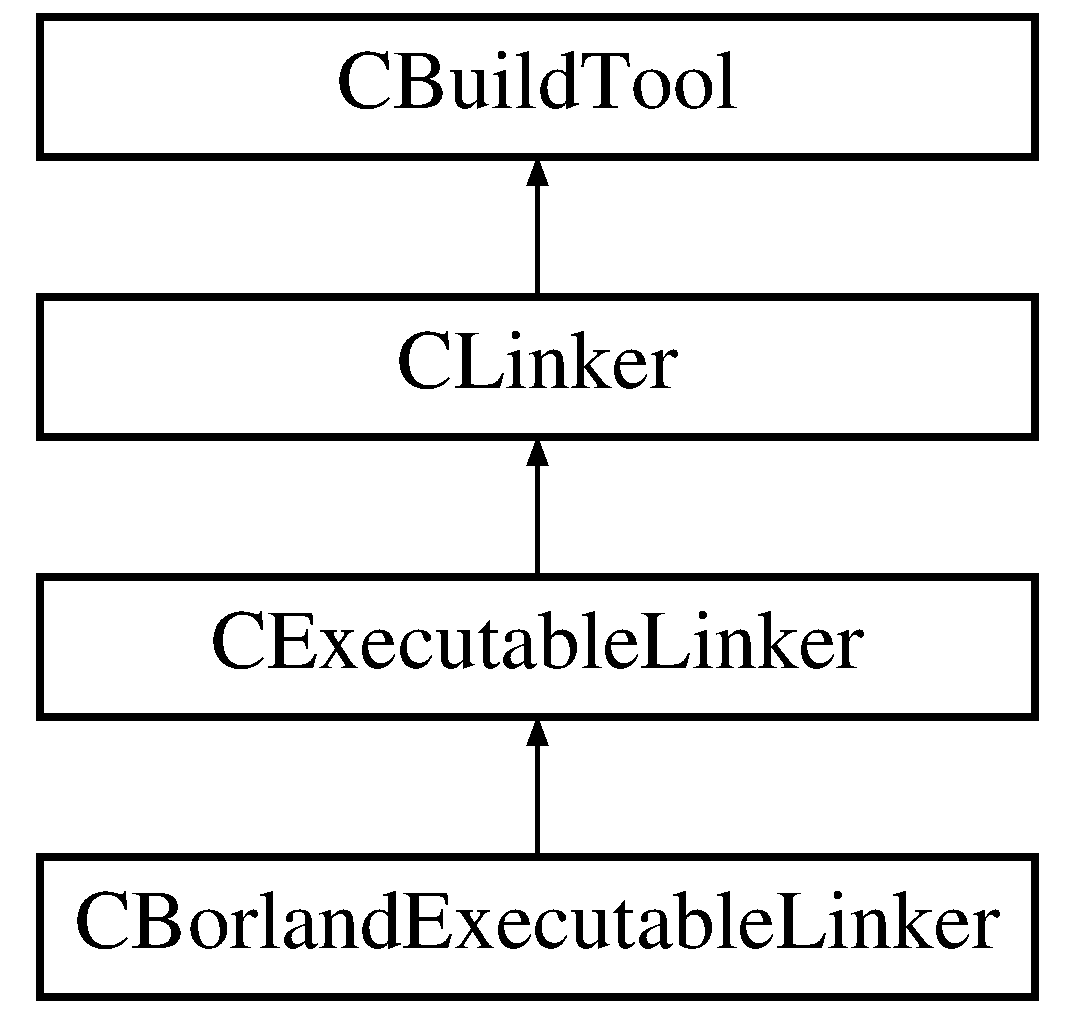
\includegraphics[height=4.000000cm]{d1/d9f/classCBorlandExecutableLinker}
\end{center}
\end{figure}
\subsection*{Public Member Functions}
\begin{DoxyCompactItemize}
\item 
virtual \hyperlink{classCBorlandExecutableLinker}{C\-Borland\-Executable\-Linker} $\ast$ \hyperlink{classCBorlandExecutableLinker_ab4acecd477ed0458760a3f14ee6fb868}{Create\-Instance} (void)
\item 
virtual void \hyperlink{classCBorlandExecutableLinker_a90ea600853600bac560530248a4a82b4}{Reset} (const \hyperlink{classCPlatform_a2fb735c63c53052f79629e338bb0f535}{C\-Platform\-::\-O\-S\-\_\-\-Type} O\-S)
\item 
virtual bool \hyperlink{classCBorlandExecutableLinker_a9786f43fd6a38bdb00fc043f069f840a}{Supports} (const \hyperlink{classCPlatform_a2fb735c63c53052f79629e338bb0f535}{C\-Platform\-::\-O\-S\-\_\-\-Type} O\-S)
\item 
\hyperlink{classCBorlandExecutableLinker_a134110e4801c569b5537670e99b9d760}{C\-Borland\-Executable\-Linker} (void)
\end{DoxyCompactItemize}
\subsection*{Additional Inherited Members}


\subsection{Constructor \& Destructor Documentation}
\hypertarget{classCBorlandExecutableLinker_a134110e4801c569b5537670e99b9d760}{\index{C\-Borland\-Executable\-Linker@{C\-Borland\-Executable\-Linker}!C\-Borland\-Executable\-Linker@{C\-Borland\-Executable\-Linker}}
\index{C\-Borland\-Executable\-Linker@{C\-Borland\-Executable\-Linker}!CBorlandExecutableLinker@{C\-Borland\-Executable\-Linker}}
\subsubsection[{C\-Borland\-Executable\-Linker}]{\setlength{\rightskip}{0pt plus 5cm}C\-Borland\-Executable\-Linker\-::\-C\-Borland\-Executable\-Linker (
\begin{DoxyParamCaption}
\item[{void}]{}
\end{DoxyParamCaption}
)}}\label{classCBorlandExecutableLinker_a134110e4801c569b5537670e99b9d760}


\subsection{Member Function Documentation}
\hypertarget{classCBorlandExecutableLinker_ab4acecd477ed0458760a3f14ee6fb868}{\index{C\-Borland\-Executable\-Linker@{C\-Borland\-Executable\-Linker}!Create\-Instance@{Create\-Instance}}
\index{Create\-Instance@{Create\-Instance}!CBorlandExecutableLinker@{C\-Borland\-Executable\-Linker}}
\subsubsection[{Create\-Instance}]{\setlength{\rightskip}{0pt plus 5cm}{\bf C\-Borland\-Executable\-Linker} $\ast$ C\-Borland\-Executable\-Linker\-::\-Create\-Instance (
\begin{DoxyParamCaption}
\item[{void}]{}
\end{DoxyParamCaption}
)\hspace{0.3cm}{\ttfamily [virtual]}}}\label{classCBorlandExecutableLinker_ab4acecd477ed0458760a3f14ee6fb868}


Reimplemented from \hyperlink{classCExecutableLinker_a457b823b737b0a78285d5ede77df827c}{C\-Executable\-Linker}.

\hypertarget{classCBorlandExecutableLinker_a90ea600853600bac560530248a4a82b4}{\index{C\-Borland\-Executable\-Linker@{C\-Borland\-Executable\-Linker}!Reset@{Reset}}
\index{Reset@{Reset}!CBorlandExecutableLinker@{C\-Borland\-Executable\-Linker}}
\subsubsection[{Reset}]{\setlength{\rightskip}{0pt plus 5cm}void C\-Borland\-Executable\-Linker\-::\-Reset (
\begin{DoxyParamCaption}
\item[{const {\bf C\-Platform\-::\-O\-S\-\_\-\-Type}}]{O\-S}
\end{DoxyParamCaption}
)\hspace{0.3cm}{\ttfamily [virtual]}}}\label{classCBorlandExecutableLinker_a90ea600853600bac560530248a4a82b4}


Reimplemented from \hyperlink{classCBuildTool_abea21a0e61ab2177effdff5aaa169585}{C\-Build\-Tool}.

\hypertarget{classCBorlandExecutableLinker_a9786f43fd6a38bdb00fc043f069f840a}{\index{C\-Borland\-Executable\-Linker@{C\-Borland\-Executable\-Linker}!Supports@{Supports}}
\index{Supports@{Supports}!CBorlandExecutableLinker@{C\-Borland\-Executable\-Linker}}
\subsubsection[{Supports}]{\setlength{\rightskip}{0pt plus 5cm}bool C\-Borland\-Executable\-Linker\-::\-Supports (
\begin{DoxyParamCaption}
\item[{const {\bf C\-Platform\-::\-O\-S\-\_\-\-Type}}]{O\-S}
\end{DoxyParamCaption}
)\hspace{0.3cm}{\ttfamily [virtual]}}}\label{classCBorlandExecutableLinker_a9786f43fd6a38bdb00fc043f069f840a}


Reimplemented from \hyperlink{classCBuildTool_ad07fcd46ccc841bc131d65505e5343c1}{C\-Build\-Tool}.



The documentation for this class was generated from the following files\-:\begin{DoxyCompactItemize}
\item 
src/\hyperlink{buildtools_8h}{buildtools.\-h}\item 
src/\hyperlink{buildtools_8cpp}{buildtools.\-cpp}\end{DoxyCompactItemize}

\hypertarget{classCBorlandResourceCompiler}{\section{C\-Borland\-Resource\-Compiler Class Reference}
\label{classCBorlandResourceCompiler}\index{C\-Borland\-Resource\-Compiler@{C\-Borland\-Resource\-Compiler}}
}


{\ttfamily \#include $<$buildtools.\-h$>$}

Inheritance diagram for C\-Borland\-Resource\-Compiler\-:\begin{figure}[H]
\begin{center}
\leavevmode
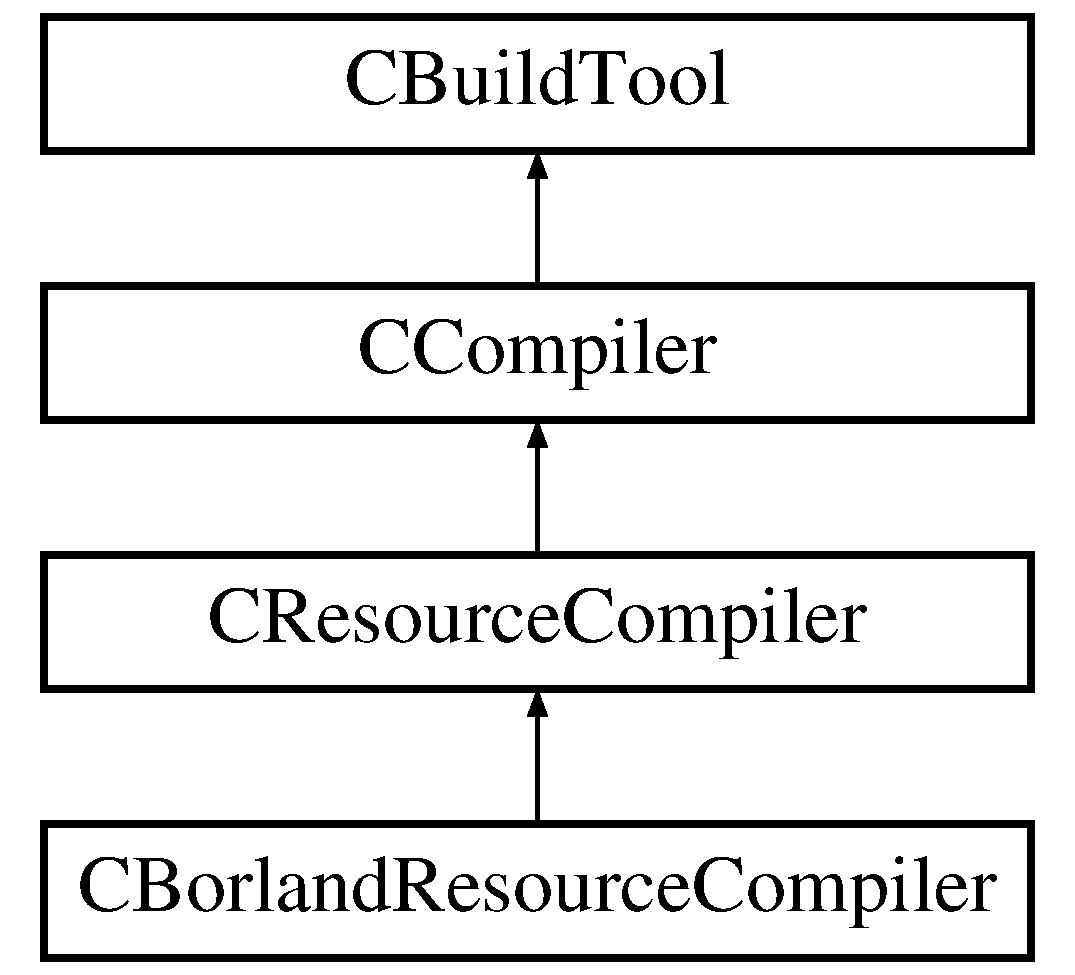
\includegraphics[height=4.000000cm]{d8/d19/classCBorlandResourceCompiler}
\end{center}
\end{figure}
\subsection*{Public Member Functions}
\begin{DoxyCompactItemize}
\item 
virtual \hyperlink{classCBorlandResourceCompiler}{C\-Borland\-Resource\-Compiler} $\ast$ \hyperlink{classCBorlandResourceCompiler_a5c6aeef4fa07fb9693feb860a70729e0}{Create\-Instance} (void)
\item 
virtual void \hyperlink{classCBorlandResourceCompiler_a586f49a9ccb4b38f3a74534eb3876c55}{Reset} (const \hyperlink{classCPlatform_a2fb735c63c53052f79629e338bb0f535}{C\-Platform\-::\-O\-S\-\_\-\-Type} O\-S)
\item 
virtual bool \hyperlink{classCBorlandResourceCompiler_a114094b4bedcad07c1986e8023ed2aca}{Supports} (const \hyperlink{classCPlatform_a2fb735c63c53052f79629e338bb0f535}{C\-Platform\-::\-O\-S\-\_\-\-Type} O\-S)
\item 
\hyperlink{classCBorlandResourceCompiler_a1407b894694903745b9e7d464ac85cbb}{C\-Borland\-Resource\-Compiler} (void)
\end{DoxyCompactItemize}
\subsection*{Additional Inherited Members}


\subsection{Constructor \& Destructor Documentation}
\hypertarget{classCBorlandResourceCompiler_a1407b894694903745b9e7d464ac85cbb}{\index{C\-Borland\-Resource\-Compiler@{C\-Borland\-Resource\-Compiler}!C\-Borland\-Resource\-Compiler@{C\-Borland\-Resource\-Compiler}}
\index{C\-Borland\-Resource\-Compiler@{C\-Borland\-Resource\-Compiler}!CBorlandResourceCompiler@{C\-Borland\-Resource\-Compiler}}
\subsubsection[{C\-Borland\-Resource\-Compiler}]{\setlength{\rightskip}{0pt plus 5cm}C\-Borland\-Resource\-Compiler\-::\-C\-Borland\-Resource\-Compiler (
\begin{DoxyParamCaption}
\item[{void}]{}
\end{DoxyParamCaption}
)}}\label{classCBorlandResourceCompiler_a1407b894694903745b9e7d464ac85cbb}


\subsection{Member Function Documentation}
\hypertarget{classCBorlandResourceCompiler_a5c6aeef4fa07fb9693feb860a70729e0}{\index{C\-Borland\-Resource\-Compiler@{C\-Borland\-Resource\-Compiler}!Create\-Instance@{Create\-Instance}}
\index{Create\-Instance@{Create\-Instance}!CBorlandResourceCompiler@{C\-Borland\-Resource\-Compiler}}
\subsubsection[{Create\-Instance}]{\setlength{\rightskip}{0pt plus 5cm}{\bf C\-Borland\-Resource\-Compiler} $\ast$ C\-Borland\-Resource\-Compiler\-::\-Create\-Instance (
\begin{DoxyParamCaption}
\item[{void}]{}
\end{DoxyParamCaption}
)\hspace{0.3cm}{\ttfamily [virtual]}}}\label{classCBorlandResourceCompiler_a5c6aeef4fa07fb9693feb860a70729e0}


Reimplemented from \hyperlink{classCResourceCompiler_a4f46ae1558a0096b040eb593d28a810c}{C\-Resource\-Compiler}.

\hypertarget{classCBorlandResourceCompiler_a586f49a9ccb4b38f3a74534eb3876c55}{\index{C\-Borland\-Resource\-Compiler@{C\-Borland\-Resource\-Compiler}!Reset@{Reset}}
\index{Reset@{Reset}!CBorlandResourceCompiler@{C\-Borland\-Resource\-Compiler}}
\subsubsection[{Reset}]{\setlength{\rightskip}{0pt plus 5cm}void C\-Borland\-Resource\-Compiler\-::\-Reset (
\begin{DoxyParamCaption}
\item[{const {\bf C\-Platform\-::\-O\-S\-\_\-\-Type}}]{O\-S}
\end{DoxyParamCaption}
)\hspace{0.3cm}{\ttfamily [virtual]}}}\label{classCBorlandResourceCompiler_a586f49a9ccb4b38f3a74534eb3876c55}


Reimplemented from \hyperlink{classCBuildTool_abea21a0e61ab2177effdff5aaa169585}{C\-Build\-Tool}.

\hypertarget{classCBorlandResourceCompiler_a114094b4bedcad07c1986e8023ed2aca}{\index{C\-Borland\-Resource\-Compiler@{C\-Borland\-Resource\-Compiler}!Supports@{Supports}}
\index{Supports@{Supports}!CBorlandResourceCompiler@{C\-Borland\-Resource\-Compiler}}
\subsubsection[{Supports}]{\setlength{\rightskip}{0pt plus 5cm}bool C\-Borland\-Resource\-Compiler\-::\-Supports (
\begin{DoxyParamCaption}
\item[{const {\bf C\-Platform\-::\-O\-S\-\_\-\-Type}}]{O\-S}
\end{DoxyParamCaption}
)\hspace{0.3cm}{\ttfamily [virtual]}}}\label{classCBorlandResourceCompiler_a114094b4bedcad07c1986e8023ed2aca}


Reimplemented from \hyperlink{classCBuildTool_ad07fcd46ccc841bc131d65505e5343c1}{C\-Build\-Tool}.



The documentation for this class was generated from the following files\-:\begin{DoxyCompactItemize}
\item 
src/\hyperlink{buildtools_8h}{buildtools.\-h}\item 
src/\hyperlink{buildtools_8cpp}{buildtools.\-cpp}\end{DoxyCompactItemize}

\hypertarget{classCBorlandStaticLinker}{\section{C\-Borland\-Static\-Linker Class Reference}
\label{classCBorlandStaticLinker}\index{C\-Borland\-Static\-Linker@{C\-Borland\-Static\-Linker}}
}


{\ttfamily \#include $<$buildtools.\-h$>$}

Inheritance diagram for C\-Borland\-Static\-Linker\-:\begin{figure}[H]
\begin{center}
\leavevmode
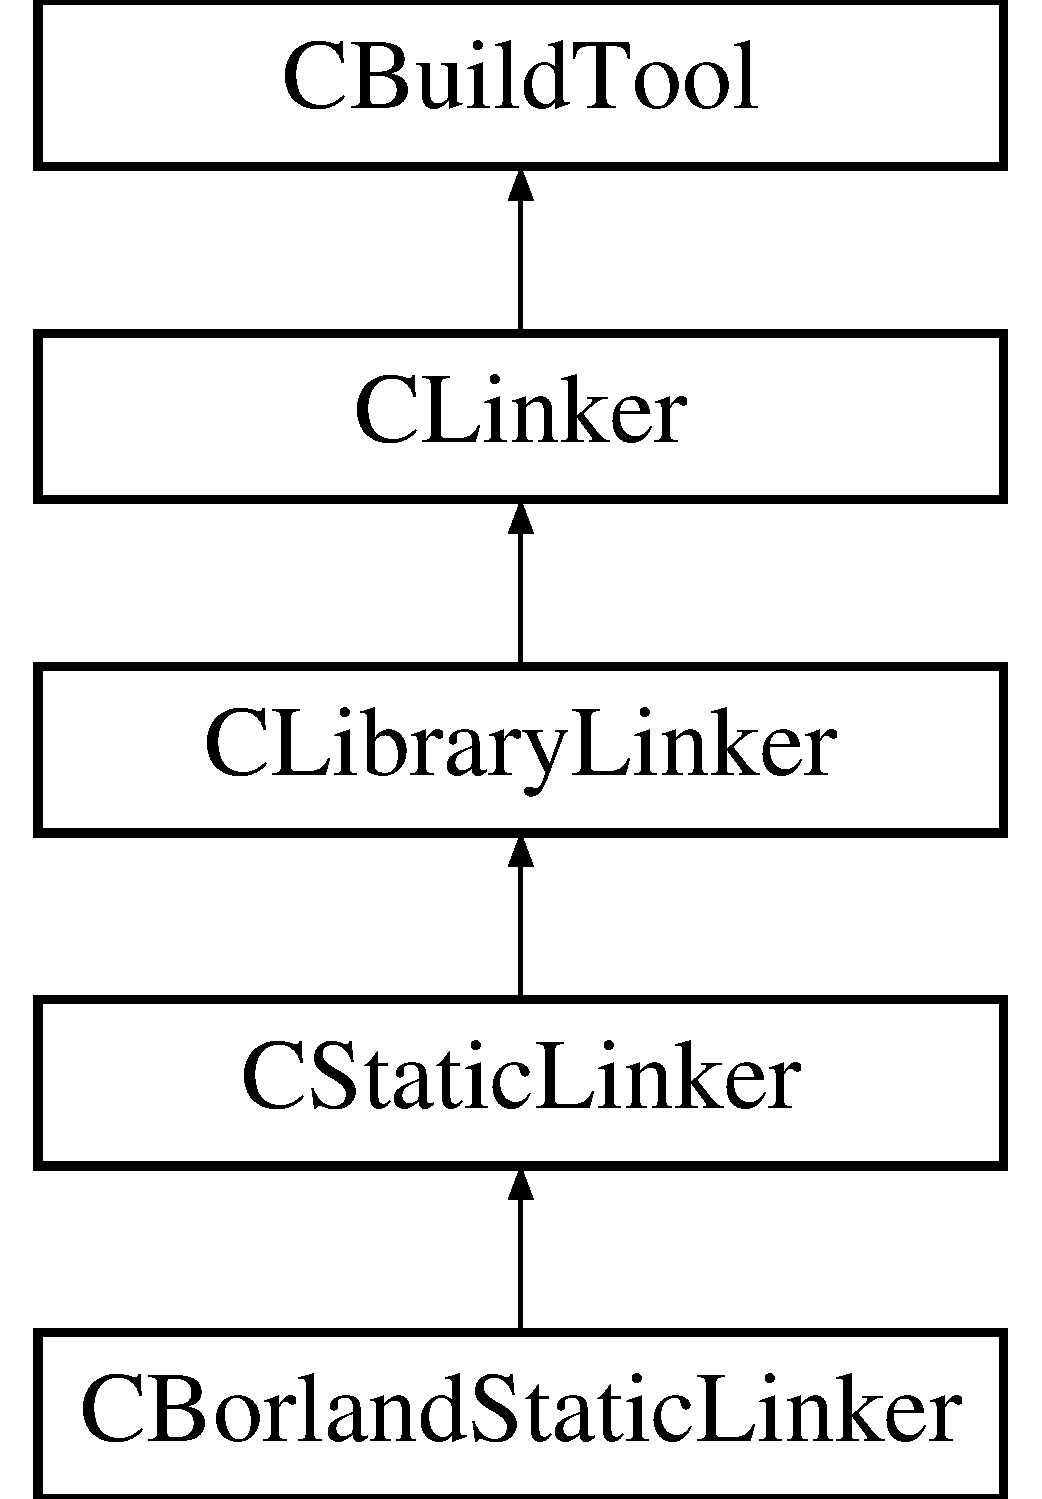
\includegraphics[height=5.000000cm]{d4/d47/classCBorlandStaticLinker}
\end{center}
\end{figure}
\subsection*{Public Member Functions}
\begin{DoxyCompactItemize}
\item 
virtual \hyperlink{classCBorlandStaticLinker}{C\-Borland\-Static\-Linker} $\ast$ \hyperlink{classCBorlandStaticLinker_ac5c637b9e4762cf272d8710be8212857}{Create\-Instance} (void)
\item 
virtual void \hyperlink{classCBorlandStaticLinker_a179338b382e0a92ccc927666c52cdf18}{Reset} (const \hyperlink{classCPlatform_a2fb735c63c53052f79629e338bb0f535}{C\-Platform\-::\-O\-S\-\_\-\-Type} O\-S)
\item 
virtual bool \hyperlink{classCBorlandStaticLinker_ad2a9e9d8203c34246ca26641fb2e941b}{Supports} (const \hyperlink{classCPlatform_a2fb735c63c53052f79629e338bb0f535}{C\-Platform\-::\-O\-S\-\_\-\-Type} O\-S)
\item 
\hyperlink{classCBorlandStaticLinker_ad22e05578c8a79007ba36b43ea29755a}{C\-Borland\-Static\-Linker} (void)
\end{DoxyCompactItemize}
\subsection*{Additional Inherited Members}


\subsection{Constructor \& Destructor Documentation}
\hypertarget{classCBorlandStaticLinker_ad22e05578c8a79007ba36b43ea29755a}{\index{C\-Borland\-Static\-Linker@{C\-Borland\-Static\-Linker}!C\-Borland\-Static\-Linker@{C\-Borland\-Static\-Linker}}
\index{C\-Borland\-Static\-Linker@{C\-Borland\-Static\-Linker}!CBorlandStaticLinker@{C\-Borland\-Static\-Linker}}
\subsubsection[{C\-Borland\-Static\-Linker}]{\setlength{\rightskip}{0pt plus 5cm}C\-Borland\-Static\-Linker\-::\-C\-Borland\-Static\-Linker (
\begin{DoxyParamCaption}
\item[{void}]{}
\end{DoxyParamCaption}
)}}\label{classCBorlandStaticLinker_ad22e05578c8a79007ba36b43ea29755a}


\subsection{Member Function Documentation}
\hypertarget{classCBorlandStaticLinker_ac5c637b9e4762cf272d8710be8212857}{\index{C\-Borland\-Static\-Linker@{C\-Borland\-Static\-Linker}!Create\-Instance@{Create\-Instance}}
\index{Create\-Instance@{Create\-Instance}!CBorlandStaticLinker@{C\-Borland\-Static\-Linker}}
\subsubsection[{Create\-Instance}]{\setlength{\rightskip}{0pt plus 5cm}{\bf C\-Borland\-Static\-Linker} $\ast$ C\-Borland\-Static\-Linker\-::\-Create\-Instance (
\begin{DoxyParamCaption}
\item[{void}]{}
\end{DoxyParamCaption}
)\hspace{0.3cm}{\ttfamily [virtual]}}}\label{classCBorlandStaticLinker_ac5c637b9e4762cf272d8710be8212857}


Reimplemented from \hyperlink{classCStaticLinker_a7e626491caa847ef207032ee600625db}{C\-Static\-Linker}.

\hypertarget{classCBorlandStaticLinker_a179338b382e0a92ccc927666c52cdf18}{\index{C\-Borland\-Static\-Linker@{C\-Borland\-Static\-Linker}!Reset@{Reset}}
\index{Reset@{Reset}!CBorlandStaticLinker@{C\-Borland\-Static\-Linker}}
\subsubsection[{Reset}]{\setlength{\rightskip}{0pt plus 5cm}void C\-Borland\-Static\-Linker\-::\-Reset (
\begin{DoxyParamCaption}
\item[{const {\bf C\-Platform\-::\-O\-S\-\_\-\-Type}}]{O\-S}
\end{DoxyParamCaption}
)\hspace{0.3cm}{\ttfamily [virtual]}}}\label{classCBorlandStaticLinker_a179338b382e0a92ccc927666c52cdf18}


Reimplemented from \hyperlink{classCBuildTool_abea21a0e61ab2177effdff5aaa169585}{C\-Build\-Tool}.

\hypertarget{classCBorlandStaticLinker_ad2a9e9d8203c34246ca26641fb2e941b}{\index{C\-Borland\-Static\-Linker@{C\-Borland\-Static\-Linker}!Supports@{Supports}}
\index{Supports@{Supports}!CBorlandStaticLinker@{C\-Borland\-Static\-Linker}}
\subsubsection[{Supports}]{\setlength{\rightskip}{0pt plus 5cm}bool C\-Borland\-Static\-Linker\-::\-Supports (
\begin{DoxyParamCaption}
\item[{const {\bf C\-Platform\-::\-O\-S\-\_\-\-Type}}]{O\-S}
\end{DoxyParamCaption}
)\hspace{0.3cm}{\ttfamily [virtual]}}}\label{classCBorlandStaticLinker_ad2a9e9d8203c34246ca26641fb2e941b}


Reimplemented from \hyperlink{classCBuildTool_ad07fcd46ccc841bc131d65505e5343c1}{C\-Build\-Tool}.



The documentation for this class was generated from the following files\-:\begin{DoxyCompactItemize}
\item 
src/\hyperlink{buildtools_8h}{buildtools.\-h}\item 
src/\hyperlink{buildtools_8cpp}{buildtools.\-cpp}\end{DoxyCompactItemize}

\hypertarget{classCBorlandToolChain}{\section{C\-Borland\-Tool\-Chain Class Reference}
\label{classCBorlandToolChain}\index{C\-Borland\-Tool\-Chain@{C\-Borland\-Tool\-Chain}}
}


{\ttfamily \#include $<$toolchains.\-h$>$}

Inheritance diagram for C\-Borland\-Tool\-Chain\-:\begin{figure}[H]
\begin{center}
\leavevmode
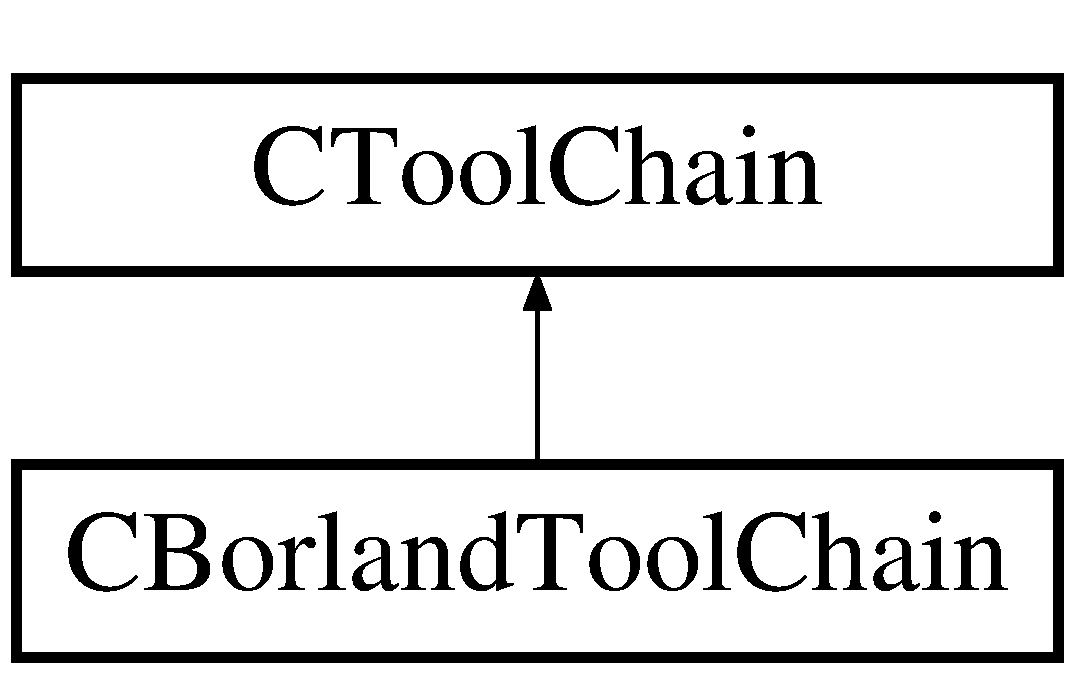
\includegraphics[height=2.000000cm]{d8/d8b/classCBorlandToolChain}
\end{center}
\end{figure}
\subsection*{Public Member Functions}
\begin{DoxyCompactItemize}
\item 
virtual \hyperlink{classCToolChain}{C\-Tool\-Chain} $\ast$ \hyperlink{classCBorlandToolChain_ae761316ad1cd0f7a4f8cdc6fa33163b0}{Create\-Instance} (void) const 
\item 
virtual void \hyperlink{classCBorlandToolChain_a25c0228c4c57d8abf968e0fb32031a55}{Reset} (const \hyperlink{classCPlatform_a2fb735c63c53052f79629e338bb0f535}{C\-Platform\-::\-O\-S\-\_\-\-Type} \hyperlink{classCToolChain_abe4054d9081351e099163e2c53b260f8}{O\-S})
\item 
\hyperlink{classCBorlandToolChain_a40792f9ab0c1042088a2aa00006b6c94}{C\-Borland\-Tool\-Chain} (void)
\item 
virtual \hyperlink{classCBorlandToolChain_ac14475f9a7aa01427c465acfa6efab25}{$\sim$\-C\-Borland\-Tool\-Chain} (void)
\end{DoxyCompactItemize}
\subsection*{Additional Inherited Members}


\subsection{Constructor \& Destructor Documentation}
\hypertarget{classCBorlandToolChain_a40792f9ab0c1042088a2aa00006b6c94}{\index{C\-Borland\-Tool\-Chain@{C\-Borland\-Tool\-Chain}!C\-Borland\-Tool\-Chain@{C\-Borland\-Tool\-Chain}}
\index{C\-Borland\-Tool\-Chain@{C\-Borland\-Tool\-Chain}!CBorlandToolChain@{C\-Borland\-Tool\-Chain}}
\subsubsection[{C\-Borland\-Tool\-Chain}]{\setlength{\rightskip}{0pt plus 5cm}C\-Borland\-Tool\-Chain\-::\-C\-Borland\-Tool\-Chain (
\begin{DoxyParamCaption}
\item[{void}]{}
\end{DoxyParamCaption}
)}}\label{classCBorlandToolChain_a40792f9ab0c1042088a2aa00006b6c94}
\hypertarget{classCBorlandToolChain_ac14475f9a7aa01427c465acfa6efab25}{\index{C\-Borland\-Tool\-Chain@{C\-Borland\-Tool\-Chain}!$\sim$\-C\-Borland\-Tool\-Chain@{$\sim$\-C\-Borland\-Tool\-Chain}}
\index{$\sim$\-C\-Borland\-Tool\-Chain@{$\sim$\-C\-Borland\-Tool\-Chain}!CBorlandToolChain@{C\-Borland\-Tool\-Chain}}
\subsubsection[{$\sim$\-C\-Borland\-Tool\-Chain}]{\setlength{\rightskip}{0pt plus 5cm}C\-Borland\-Tool\-Chain\-::$\sim$\-C\-Borland\-Tool\-Chain (
\begin{DoxyParamCaption}
\item[{void}]{}
\end{DoxyParamCaption}
)\hspace{0.3cm}{\ttfamily [virtual]}}}\label{classCBorlandToolChain_ac14475f9a7aa01427c465acfa6efab25}


\subsection{Member Function Documentation}
\hypertarget{classCBorlandToolChain_ae761316ad1cd0f7a4f8cdc6fa33163b0}{\index{C\-Borland\-Tool\-Chain@{C\-Borland\-Tool\-Chain}!Create\-Instance@{Create\-Instance}}
\index{Create\-Instance@{Create\-Instance}!CBorlandToolChain@{C\-Borland\-Tool\-Chain}}
\subsubsection[{Create\-Instance}]{\setlength{\rightskip}{0pt plus 5cm}{\bf C\-Tool\-Chain} $\ast$ C\-Borland\-Tool\-Chain\-::\-Create\-Instance (
\begin{DoxyParamCaption}
\item[{void}]{}
\end{DoxyParamCaption}
) const\hspace{0.3cm}{\ttfamily [virtual]}}}\label{classCBorlandToolChain_ae761316ad1cd0f7a4f8cdc6fa33163b0}


Reimplemented from \hyperlink{classCToolChain_aa6765d5197d898efb01d032ac73b7764}{C\-Tool\-Chain}.

\hypertarget{classCBorlandToolChain_a25c0228c4c57d8abf968e0fb32031a55}{\index{C\-Borland\-Tool\-Chain@{C\-Borland\-Tool\-Chain}!Reset@{Reset}}
\index{Reset@{Reset}!CBorlandToolChain@{C\-Borland\-Tool\-Chain}}
\subsubsection[{Reset}]{\setlength{\rightskip}{0pt plus 5cm}void C\-Borland\-Tool\-Chain\-::\-Reset (
\begin{DoxyParamCaption}
\item[{const {\bf C\-Platform\-::\-O\-S\-\_\-\-Type}}]{O\-S}
\end{DoxyParamCaption}
)\hspace{0.3cm}{\ttfamily [virtual]}}}\label{classCBorlandToolChain_a25c0228c4c57d8abf968e0fb32031a55}


Reimplemented from \hyperlink{classCToolChain_a3b48ddb23b898b3b6eaa356a2ed6fbf8}{C\-Tool\-Chain}.



The documentation for this class was generated from the following files\-:\begin{DoxyCompactItemize}
\item 
src/\hyperlink{toolchains_8h}{toolchains.\-h}\item 
src/\hyperlink{toolchains_8cpp}{toolchains.\-cpp}\end{DoxyCompactItemize}

\hypertarget{classCBuildManager}{\section{C\-Build\-Manager Class Reference}
\label{classCBuildManager}\index{C\-Build\-Manager@{C\-Build\-Manager}}
}


{\ttfamily \#include $<$buildtools.\-h$>$}

Inheritance diagram for C\-Build\-Manager\-:\begin{figure}[H]
\begin{center}
\leavevmode
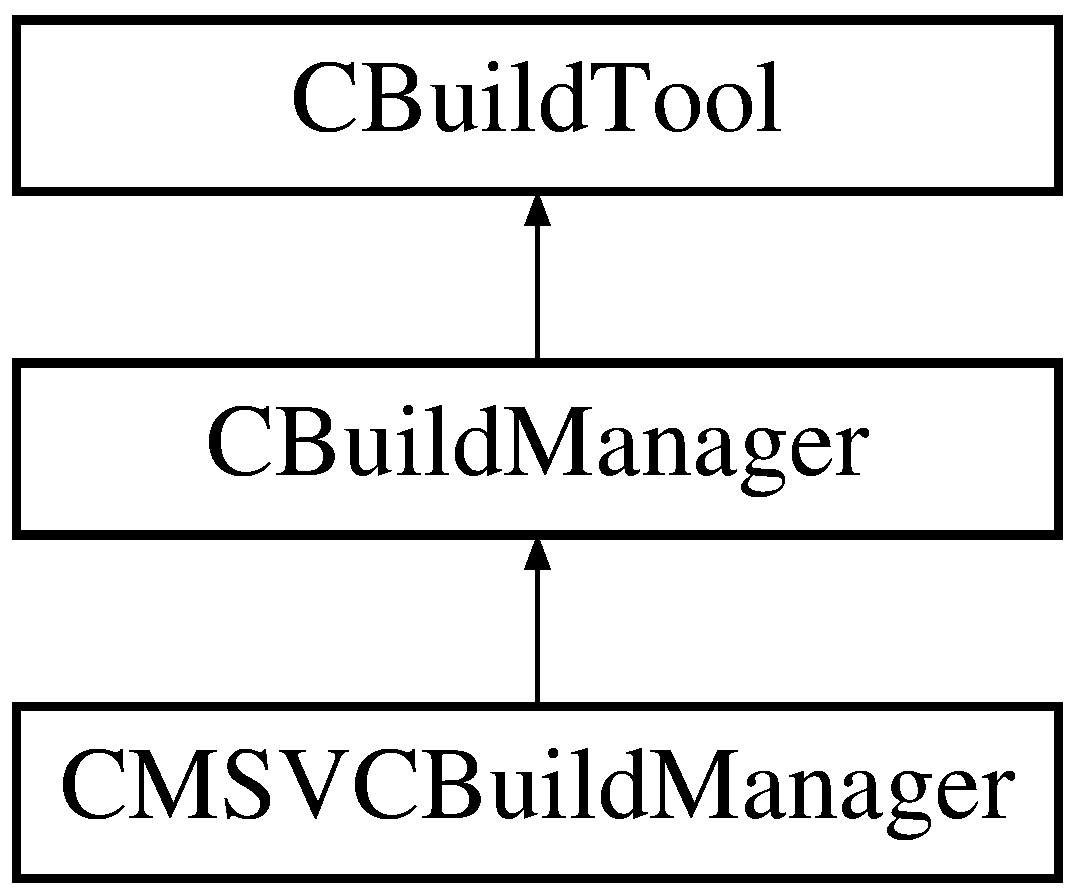
\includegraphics[height=3.000000cm]{dd/dda/classCBuildManager}
\end{center}
\end{figure}
\subsection*{Public Member Functions}
\begin{DoxyCompactItemize}
\item 
virtual \hyperlink{classCBuildManager}{C\-Build\-Manager} $\ast$ \hyperlink{classCBuildManager_a3613cf27c028cb883a5b309a8c024d75}{Create\-Instance} (void)
\item 
virtual void \hyperlink{classCBuildManager_a3a2dfa7800c44b7122a248d32dffe193}{Read} (const Ti\-Xml\-Element $\ast$Build\-Tool\-Root)
\item 
virtual void \hyperlink{classCBuildManager_a62bfb161da5eacc3b372c220dc89fa0b}{Write} (Ti\-Xml\-Element $\ast$Build\-Tool\-Root)
\item 
virtual void \hyperlink{classCBuildManager_a6a7e968c30cef765316d06a1f0a6d76c}{Show} (void)
\item 
\hyperlink{classCBuildManager_a0cd9e816598b01abb1feb74053ae009d}{C\-Build\-Manager} (void)
\item 
\hyperlink{classCBuildManager_a1cce01b779f158fb141e86be5a1dd53a}{C\-Build\-Manager} (const \hyperlink{classCBuildManager}{C\-Build\-Manager} \&Build\-Manager)
\item 
virtual \hyperlink{classCBuildManager_a5f19b138a427a10eb57911819e5bc6aa}{$\sim$\-C\-Build\-Manager} (void)
\end{DoxyCompactItemize}
\subsection*{Additional Inherited Members}


\subsection{Constructor \& Destructor Documentation}
\hypertarget{classCBuildManager_a0cd9e816598b01abb1feb74053ae009d}{\index{C\-Build\-Manager@{C\-Build\-Manager}!C\-Build\-Manager@{C\-Build\-Manager}}
\index{C\-Build\-Manager@{C\-Build\-Manager}!CBuildManager@{C\-Build\-Manager}}
\subsubsection[{C\-Build\-Manager}]{\setlength{\rightskip}{0pt plus 5cm}C\-Build\-Manager\-::\-C\-Build\-Manager (
\begin{DoxyParamCaption}
\item[{void}]{}
\end{DoxyParamCaption}
)}}\label{classCBuildManager_a0cd9e816598b01abb1feb74053ae009d}
\hypertarget{classCBuildManager_a1cce01b779f158fb141e86be5a1dd53a}{\index{C\-Build\-Manager@{C\-Build\-Manager}!C\-Build\-Manager@{C\-Build\-Manager}}
\index{C\-Build\-Manager@{C\-Build\-Manager}!CBuildManager@{C\-Build\-Manager}}
\subsubsection[{C\-Build\-Manager}]{\setlength{\rightskip}{0pt plus 5cm}C\-Build\-Manager\-::\-C\-Build\-Manager (
\begin{DoxyParamCaption}
\item[{const {\bf C\-Build\-Manager} \&}]{Build\-Manager}
\end{DoxyParamCaption}
)}}\label{classCBuildManager_a1cce01b779f158fb141e86be5a1dd53a}
\hypertarget{classCBuildManager_a5f19b138a427a10eb57911819e5bc6aa}{\index{C\-Build\-Manager@{C\-Build\-Manager}!$\sim$\-C\-Build\-Manager@{$\sim$\-C\-Build\-Manager}}
\index{$\sim$\-C\-Build\-Manager@{$\sim$\-C\-Build\-Manager}!CBuildManager@{C\-Build\-Manager}}
\subsubsection[{$\sim$\-C\-Build\-Manager}]{\setlength{\rightskip}{0pt plus 5cm}C\-Build\-Manager\-::$\sim$\-C\-Build\-Manager (
\begin{DoxyParamCaption}
\item[{void}]{}
\end{DoxyParamCaption}
)\hspace{0.3cm}{\ttfamily [virtual]}}}\label{classCBuildManager_a5f19b138a427a10eb57911819e5bc6aa}


\subsection{Member Function Documentation}
\hypertarget{classCBuildManager_a3613cf27c028cb883a5b309a8c024d75}{\index{C\-Build\-Manager@{C\-Build\-Manager}!Create\-Instance@{Create\-Instance}}
\index{Create\-Instance@{Create\-Instance}!CBuildManager@{C\-Build\-Manager}}
\subsubsection[{Create\-Instance}]{\setlength{\rightskip}{0pt plus 5cm}{\bf C\-Build\-Manager} $\ast$ C\-Build\-Manager\-::\-Create\-Instance (
\begin{DoxyParamCaption}
\item[{void}]{}
\end{DoxyParamCaption}
)\hspace{0.3cm}{\ttfamily [virtual]}}}\label{classCBuildManager_a3613cf27c028cb883a5b309a8c024d75}


Reimplemented from \hyperlink{classCBuildTool_aa7f0e7c0bd7f75c71d37df066bcb581e}{C\-Build\-Tool}.



Reimplemented in \hyperlink{classCMSVCBuildManager_a2519f0cd2477b6f9bd4459b15635c466}{C\-M\-S\-V\-C\-Build\-Manager}.

\hypertarget{classCBuildManager_a3a2dfa7800c44b7122a248d32dffe193}{\index{C\-Build\-Manager@{C\-Build\-Manager}!Read@{Read}}
\index{Read@{Read}!CBuildManager@{C\-Build\-Manager}}
\subsubsection[{Read}]{\setlength{\rightskip}{0pt plus 5cm}void C\-Build\-Manager\-::\-Read (
\begin{DoxyParamCaption}
\item[{const Ti\-Xml\-Element $\ast$}]{Build\-Tool\-Root}
\end{DoxyParamCaption}
)\hspace{0.3cm}{\ttfamily [virtual]}}}\label{classCBuildManager_a3a2dfa7800c44b7122a248d32dffe193}


Reimplemented from \hyperlink{classCBuildTool_a299d87943c0f68dde5316318cc0838f8}{C\-Build\-Tool}.

\hypertarget{classCBuildManager_a6a7e968c30cef765316d06a1f0a6d76c}{\index{C\-Build\-Manager@{C\-Build\-Manager}!Show@{Show}}
\index{Show@{Show}!CBuildManager@{C\-Build\-Manager}}
\subsubsection[{Show}]{\setlength{\rightskip}{0pt plus 5cm}void C\-Build\-Manager\-::\-Show (
\begin{DoxyParamCaption}
\item[{void}]{}
\end{DoxyParamCaption}
)\hspace{0.3cm}{\ttfamily [virtual]}}}\label{classCBuildManager_a6a7e968c30cef765316d06a1f0a6d76c}


Reimplemented from \hyperlink{classCBuildTool_a69815d1393a61dc16b2cc2d0552cd5ac}{C\-Build\-Tool}.

\hypertarget{classCBuildManager_a62bfb161da5eacc3b372c220dc89fa0b}{\index{C\-Build\-Manager@{C\-Build\-Manager}!Write@{Write}}
\index{Write@{Write}!CBuildManager@{C\-Build\-Manager}}
\subsubsection[{Write}]{\setlength{\rightskip}{0pt plus 5cm}void C\-Build\-Manager\-::\-Write (
\begin{DoxyParamCaption}
\item[{Ti\-Xml\-Element $\ast$}]{Build\-Tool\-Root}
\end{DoxyParamCaption}
)\hspace{0.3cm}{\ttfamily [virtual]}}}\label{classCBuildManager_a62bfb161da5eacc3b372c220dc89fa0b}


Reimplemented from \hyperlink{classCBuildTool_af0331a777785bc2d15236b5c74321ed2}{C\-Build\-Tool}.



The documentation for this class was generated from the following files\-:\begin{DoxyCompactItemize}
\item 
src/\hyperlink{buildtools_8h}{buildtools.\-h}\item 
src/\hyperlink{buildtools_8cpp}{buildtools.\-cpp}\end{DoxyCompactItemize}

\hypertarget{classCBuildTarget}{\section{C\-Build\-Target Class Reference}
\label{classCBuildTarget}\index{C\-Build\-Target@{C\-Build\-Target}}
}


{\ttfamily \#include $<$cbptarget.\-h$>$}

\subsection*{Public Types}
\begin{DoxyCompactItemize}
\item 
enum \hyperlink{classCBuildTarget_ae920f5ba8e1975bafff70b8b30c449b5}{Target\-Type} \{ \\*
\hyperlink{classCBuildTarget_ae920f5ba8e1975bafff70b8b30c449b5a2f28239e2aa020ac7b599abfd8cb80ed}{tt\-Executable}, 
\hyperlink{classCBuildTarget_ae920f5ba8e1975bafff70b8b30c449b5a2cec686fb122a44a2c4bf79a2fadd7c6}{tt\-Console\-Executable}, 
\hyperlink{classCBuildTarget_ae920f5ba8e1975bafff70b8b30c449b5a0f87b6b58d86a799d1d8bd570ecc74d2}{tt\-Static\-Library}, 
\hyperlink{classCBuildTarget_ae920f5ba8e1975bafff70b8b30c449b5a946ebe00dc38daf8c11dfdeb3a1fda7e}{tt\-Dynamic\-Library}, 
\\*
\hyperlink{classCBuildTarget_ae920f5ba8e1975bafff70b8b30c449b5ae3df2a57236e2f98f3f9c0c5ce631a80}{tt\-Commands}, 
\hyperlink{classCBuildTarget_ae920f5ba8e1975bafff70b8b30c449b5a023882bf682aef975e3f1f8283f51746}{tt\-Native}
 \}
\item 
enum \hyperlink{classCBuildTarget_a65a8d160e9cb9cc5632373836e0adb9e}{Options\-Relation} \{ \hyperlink{classCBuildTarget_a65a8d160e9cb9cc5632373836e0adb9ea8dbc1b5fb7384bcacc5453576eb53e9c}{or\-Project}, 
\hyperlink{classCBuildTarget_a65a8d160e9cb9cc5632373836e0adb9ea8f001181cd9f7aaa76e8915b27bef01a}{or\-Target}, 
\hyperlink{classCBuildTarget_a65a8d160e9cb9cc5632373836e0adb9eaee0e19bc748d10d35c664671fc5547a6}{or\-Target\-Project}, 
\hyperlink{classCBuildTarget_a65a8d160e9cb9cc5632373836e0adb9ea7ca6ec2ac0853a0516a4638cd2aaf391}{or\-Project\-Target}
 \}
\end{DoxyCompactItemize}
\subsection*{Public Member Functions}
\begin{DoxyCompactItemize}
\item 
\hyperlink{classCString}{C\-String} \hyperlink{classCBuildTarget_a997ce9f51676fc0af256fb9589801250}{Title} (void) const 
\item 
\hyperlink{classCStringList}{C\-String\-List} \hyperlink{classCBuildTarget_a58751895acaacab3b76e580c1d43a355}{Platforms} (void) const 
\item 
\hyperlink{classCString}{C\-String} \hyperlink{classCBuildTarget_a55dc82877928bf87905a3b2073d2fe31}{Output} (void) const 
\item 
\hyperlink{classCString}{C\-String} \hyperlink{classCBuildTarget_a47d5e653d7bdb868c333e55aa075a937}{Object\-Output} (void) const 
\item 
\hyperlink{classCBuildTarget_ae920f5ba8e1975bafff70b8b30c449b5}{Target\-Type} \hyperlink{classCBuildTarget_a32caa3497047c676e850c3717b3f415b}{Type} (void) const 
\item 
bool \hyperlink{classCBuildTarget_a98a6c0e251b22eb8022cc4527fe48c30}{Auto\-Prefix} (void) const 
\item 
bool \hyperlink{classCBuildTarget_addde823ff741dbb1d264ee2c6096ac61}{Auto\-Extension} (void) const 
\item 
\hyperlink{classCString}{C\-String} \hyperlink{classCBuildTarget_aa98b9abac09952b015ecf64ac7d334f6}{Compiler} (void) const 
\item 
\hyperlink{classCStringList}{C\-String\-List} \hyperlink{classCBuildTarget_a94cce7fd363469cc115167b95605355a}{Compiler\-Directories} (void) const 
\item 
\hyperlink{classCStringList}{C\-String\-List} \hyperlink{classCBuildTarget_a11e8ebc43f32e0af7d887f629a833c9e}{Before\-Build\-Commands} (void) const 
\item 
\hyperlink{classCStringList}{C\-String\-List} \hyperlink{classCBuildTarget_acd09dfbbff2a95ae6a2124e5c925888b}{After\-Build\-Commands} (void) const 
\item 
bool \hyperlink{classCBuildTarget_a1792d9a7d96bbf5cc70168843be26f97}{Force\-Before\-Build\-Commands} (void) const 
\item 
bool \hyperlink{classCBuildTarget_a036630435ab61878316b4025d2588f1b}{Force\-After\-Build\-Commands} (void) const 
\item 
int \& \hyperlink{classCBuildTarget_ab907802acd72029fe1755d2693f4840e}{Name\-Case} (void)
\item 
\hyperlink{classCString}{C\-String} \hyperlink{classCBuildTarget_af4c548db9ccae0723b8e2a5d0ee2e854}{U\-C\-Name} (void) const 
\item 
\hyperlink{classCString}{C\-String} \hyperlink{classCBuildTarget_a176a192632b102d9fe7f13e74dec4ab1}{L\-C\-Name} (void) const 
\item 
\hyperlink{classCString}{C\-String} \hyperlink{classCBuildTarget_aa454818e8e930ceeca534be7dfd1d291}{M\-F\-Name} (void) const 
\item 
\hyperlink{classCString}{C\-String} \hyperlink{classCBuildTarget_a9ed0f8434aa864c81b92a2f9e8179592}{Name} (const \hyperlink{classCString}{C\-String} \&Prefix, const int Case) const 
\item 
\hyperlink{classCString}{C\-String} \hyperlink{classCBuildTarget_a0a63f43a245d3847de658c04bab2a779}{Name} (const \hyperlink{classCString}{C\-String} \&Prefix) const 
\item 
\hyperlink{classCString}{C\-String} \hyperlink{classCBuildTarget_a151fe2c898a726d018f55ecd29f865c6}{Target\-Type\-Name} (const \hyperlink{classCBuildTarget_ae920f5ba8e1975bafff70b8b30c449b5}{Target\-Type} \hyperlink{classCBuildTarget_a32caa3497047c676e850c3717b3f415b}{Type})
\item 
\hyperlink{classCString}{C\-String} \hyperlink{classCBuildTarget_aebe5457c8264e962905e36f320742709}{Target\-Type\-Name} (void)
\item 
\hyperlink{classCString}{C\-String} \hyperlink{classCBuildTarget_a88a8ee3495b4e0fa95cc374107284038}{Options\-Relation\-Name} (const \hyperlink{classCBuildTarget_a65a8d160e9cb9cc5632373836e0adb9e}{Options\-Relation} Relation)
\item 
\hyperlink{classCString}{C\-String} \hyperlink{classCBuildTarget_a826b64b7e824094d5d89d278577603ca}{Auto\-File\-Prefix} (const \hyperlink{classCPlatform_a2fb735c63c53052f79629e338bb0f535}{C\-Platform\-::\-O\-S\-\_\-\-Type} O\-S)
\item 
\hyperlink{classCString}{C\-String} \hyperlink{classCBuildTarget_af52379dd5436153f96c154a267f44863}{Auto\-File\-Extension} (const \hyperlink{classCPlatform_a2fb735c63c53052f79629e338bb0f535}{C\-Platform\-::\-O\-S\-\_\-\-Type} O\-S, const \hyperlink{classCBuildTarget_ae920f5ba8e1975bafff70b8b30c449b5}{C\-Build\-Target\-::\-Target\-Type} \hyperlink{classCBuildTarget_a32caa3497047c676e850c3717b3f415b}{Type})
\item 
\hyperlink{classCString}{C\-String} \hyperlink{classCBuildTarget_acd5c16cc0c6d0b9cbba7643ab7ba5f66}{Auto\-File\-Extension} (\hyperlink{classCString}{C\-String} \&Platform)
\item 
\hyperlink{classCString}{C\-String} \hyperlink{classCBuildTarget_ac202a744e5ce09fff6a7c5b069d4d472}{Auto\-File\-Extension} (const int Platform)
\item 
\hyperlink{classCString}{C\-String} \hyperlink{classCBuildTarget_a0a5b72aec11a5557a4cdab09c80cf398}{Make\-Options} (const \hyperlink{classCBuildTarget_a65a8d160e9cb9cc5632373836e0adb9e}{Options\-Relation} Relation, const \hyperlink{classCString}{C\-String} \&Project\-Options, const \hyperlink{classCString}{C\-String} \&Target\-Options)
\item 
\hyperlink{classCString}{C\-String} \hyperlink{classCBuildTarget_a01596962482210ddf57c073c3d2d5a79}{C\-Flags} (void)
\item 
\hyperlink{classCString}{C\-String} \hyperlink{classCBuildTarget_a346e7b7ef105a1e471e30fb1a2334efd}{C\-Flags} (const \hyperlink{classCString}{C\-String} \&Project\-C\-Flags)
\item 
\hyperlink{classCString}{C\-String} \hyperlink{classCBuildTarget_a95adb69caa6182e6817d1766e3800e5a}{R\-C\-Flags} (void)
\item 
\hyperlink{classCString}{C\-String} \hyperlink{classCBuildTarget_a0ea25f287154d79acb94d2ce79d34c01}{R\-C\-Flags} (const \hyperlink{classCString}{C\-String} \&Project\-R\-C\-Flags)
\item 
\hyperlink{classCString}{C\-String} \hyperlink{classCBuildTarget_a126b179e98d25123a27e515e4e35e9c4}{Ld\-Flags} (void)
\item 
\hyperlink{classCString}{C\-String} \hyperlink{classCBuildTarget_ab0fef1c7a4e9e6a7a7e3f3fa80d5af9a}{Ld\-Flags} (const \hyperlink{classCString}{C\-String} \&Project\-Ld\-Flags)
\item 
\hyperlink{classCString}{C\-String} \hyperlink{classCBuildTarget_aa5f434c9bee3c8bc1d1491497ab476fc}{Inc\-Dirs} (const \hyperlink{classCString}{C\-String} \&Inc\-Dir\-Switch)
\item 
\hyperlink{classCString}{C\-String} \hyperlink{classCBuildTarget_af7d3a568a1b326749c6fa9e003046b64}{Inc\-Dirs} (const \hyperlink{classCString}{C\-String} \&Project\-Inc\-Dirs, const \hyperlink{classCString}{C\-String} \&Inc\-Dir\-Switch)
\item 
\hyperlink{classCString}{C\-String} \hyperlink{classCBuildTarget_aa3126d4d24703558a4434b1a2c24f54c}{Res\-Dirs} (const \hyperlink{classCString}{C\-String} \&Inc\-Dir\-Switch)
\item 
\hyperlink{classCString}{C\-String} \hyperlink{classCBuildTarget_a50897314665969727bf7e9eef4d68a11}{Res\-Dirs} (const \hyperlink{classCString}{C\-String} \&Project\-Res\-Dirs, const \hyperlink{classCString}{C\-String} \&Inc\-Dir\-Switch)
\item 
\hyperlink{classCString}{C\-String} \hyperlink{classCBuildTarget_a5b0d1db0c9a71baf75948a1023e1ac3e}{Lib\-Dirs} (const \hyperlink{classCString}{C\-String} \&Lib\-Dir\-Switch)
\item 
\hyperlink{classCString}{C\-String} \hyperlink{classCBuildTarget_a9d8910a1f0d25902d91f1937e561dafd}{Lib\-Dirs} (const \hyperlink{classCString}{C\-String} \&Project\-Lib\-Dirs, const \hyperlink{classCString}{C\-String} \&Lib\-Dir\-Switch)
\item 
\hyperlink{classCString}{C\-String} \hyperlink{classCBuildTarget_ab8e4e6c34baedfe4880d73082e76d2cb}{Libs} (const \hyperlink{classCPlatform}{C\-Platform} \&Platform, const \hyperlink{classCString}{C\-String} \&Link\-Lib\-Switch)
\item 
\hyperlink{classCString}{C\-String} \hyperlink{classCBuildTarget_ac2d634a30fc74759b6b60db521850fe1}{Ext\-Deps} (void)
\item 
void \hyperlink{classCBuildTarget_a8a657acbe3b7114de59e98449ba8c98f}{Clear} (void)
\item 
void \hyperlink{classCBuildTarget_a202834e8685ab0be83aec5c76b326635}{Read} (const Ti\-Xml\-Element $\ast$Target\-Root)
\item 
void \hyperlink{classCBuildTarget_a57954e30f73ed40c0cac432e3d9e285b}{Show} (void)
\item 
\hyperlink{classCBuildTarget_a343f61a41744c3af9144da18302b8004}{C\-Build\-Target} (void)
\item 
\hyperlink{classCBuildTarget_a17c267cb329955e3a0832d931cbe2ffd}{$\sim$\-C\-Build\-Target} (void)
\end{DoxyCompactItemize}
\subsection*{Private Attributes}
\begin{DoxyCompactItemize}
\item 
\hyperlink{classCString}{C\-String} \hyperlink{classCBuildTarget_abd914af1350302b3cc592cf391d7f4a6}{m\-\_\-\-Title}
\item 
\hyperlink{classCStringList}{C\-String\-List} \hyperlink{classCBuildTarget_ac81df46e239c54c29fb4a19227f863bd}{m\-\_\-\-Platforms}
\item 
\hyperlink{classCString}{C\-String} \hyperlink{classCBuildTarget_a72308b1052dc4d1d0f50869956a0c14a}{m\-\_\-\-Output}
\item 
\hyperlink{classCString}{C\-String} \hyperlink{classCBuildTarget_afbb0bbec05f775062ba32c59560d3e52}{m\-\_\-\-Working\-Directory}
\item 
\hyperlink{classCString}{C\-String} \hyperlink{classCBuildTarget_ae9c897e9a42d93f9f66c704dad17eff1}{m\-\_\-\-Object\-Output}
\item 
\hyperlink{classCStringList}{C\-String\-List} \hyperlink{classCBuildTarget_a00c0dea4b0dd9e34fcfa540c7b8e7ee6}{m\-\_\-\-External\-Dependencies}
\item 
\hyperlink{classCBuildTarget_ae920f5ba8e1975bafff70b8b30c449b5}{Target\-Type} \hyperlink{classCBuildTarget_abdb459bba568451a5e97ff1974ab37d9}{m\-\_\-\-Type}
\item 
bool \hyperlink{classCBuildTarget_aec313b6a7d9f698ab1050fbc0a8b0ebe}{m\-\_\-\-Auto\-Prefix}
\item 
bool \hyperlink{classCBuildTarget_a9f06bf4c3b73ce8bbbab046d819e1046}{m\-\_\-\-Auto\-Extension}
\item 
\hyperlink{classCString}{C\-String} \hyperlink{classCBuildTarget_a130624eb072925fa6e104339f3cef7d3}{m\-\_\-\-Compiler}
\item 
\hyperlink{classCStringList}{C\-String\-List} \hyperlink{classCBuildTarget_a3485b4444afdf7c26edb9139fa7bfa42}{m\-\_\-\-Compiler\-Options}
\item 
\hyperlink{classCStringList}{C\-String\-List} \hyperlink{classCBuildTarget_a290af88d76bcaf78db02e3c3567c8fe8}{m\-\_\-\-Compiler\-Directories}
\item 
\hyperlink{classCStringList}{C\-String\-List} \hyperlink{classCBuildTarget_a7b691145075fb0ab23c4a1f9e26e3000}{m\-\_\-\-Linker\-Options}
\item 
\hyperlink{classCStringList}{C\-String\-List} \hyperlink{classCBuildTarget_abb6557d00a351f4b41841858c55b82f6}{m\-\_\-\-Linker\-Libraries}
\item 
\hyperlink{classCStringList}{C\-String\-List} \hyperlink{classCBuildTarget_a8495121b03ecf4a7090ce3b712d0f13c}{m\-\_\-\-Linker\-Directories}
\item 
\hyperlink{classCStringList}{C\-String\-List} \hyperlink{classCBuildTarget_a388bfb990949692aa8744bb6923cf3fa}{m\-\_\-\-Before\-Build\-Commands}
\item 
\hyperlink{classCStringList}{C\-String\-List} \hyperlink{classCBuildTarget_a55cab6b25077cc64bfc7ac3487015407}{m\-\_\-\-After\-Build\-Commands}
\item 
bool \hyperlink{classCBuildTarget_a37ce43cd33d313194cd27aed4eaf1538}{m\-\_\-\-Force\-Before\-Build\-Commands}
\item 
bool \hyperlink{classCBuildTarget_a01e842edbeb72632cd2216a0957f8b93}{m\-\_\-\-Force\-After\-Build\-Commands}
\item 
\hyperlink{classCStringList}{C\-String\-List} \hyperlink{classCBuildTarget_aa2a1ff76b82d5b589e771bcda8a7c0d3}{m\-\_\-\-Resource\-Compiler\-Directories}
\item 
\hyperlink{classCStringList}{C\-String\-List} \hyperlink{classCBuildTarget_a6eb47859ebf84e5baa9410348df4c42c}{m\-\_\-\-Resource\-Compiler\-Options}
\item 
\hyperlink{classCBuildTarget_a65a8d160e9cb9cc5632373836e0adb9e}{Options\-Relation} \hyperlink{classCBuildTarget_a91e76527d772e1df848b78e5264774af}{m\-\_\-\-Compiler\-Options\-Relation}
\item 
\hyperlink{classCBuildTarget_a65a8d160e9cb9cc5632373836e0adb9e}{Options\-Relation} \hyperlink{classCBuildTarget_a88376156248b785211fa8ee8751b19e8}{m\-\_\-\-Linker\-Options\-Relation}
\item 
\hyperlink{classCBuildTarget_a65a8d160e9cb9cc5632373836e0adb9e}{Options\-Relation} \hyperlink{classCBuildTarget_a0e09642183809d9395d0573f8b1afd9d}{m\-\_\-\-Include\-Directories\-Relation}
\item 
\hyperlink{classCBuildTarget_a65a8d160e9cb9cc5632373836e0adb9e}{Options\-Relation} \hyperlink{classCBuildTarget_aaa250c58cf7203b795544a809773d230}{m\-\_\-\-Resource\-Include\-Directories\-Relation}
\item 
\hyperlink{classCBuildTarget_a65a8d160e9cb9cc5632373836e0adb9e}{Options\-Relation} \hyperlink{classCBuildTarget_a7febe49001f7362e21d170e918ced09f}{m\-\_\-\-Library\-Directories\-Relation}
\item 
\hyperlink{classCBuildTarget_a65a8d160e9cb9cc5632373836e0adb9e}{Options\-Relation} \hyperlink{classCBuildTarget_a6e41481ecb82a7ddc114be1e420fd960}{m\-\_\-\-Resource\-Compiler\-Options\-Relation}
\item 
int \hyperlink{classCBuildTarget_a046e2fd1be16b46b33bde0edc0f275c4}{m\-\_\-\-Name\-Case}
\item 
\hyperlink{classCString}{C\-String} \hyperlink{classCBuildTarget_ab3da058a427da4e7a16f138d35150b62}{m\-\_\-\-U\-C\-Name}
\item 
\hyperlink{classCString}{C\-String} \hyperlink{classCBuildTarget_a1cc23d76e72157889515dfbf6d682ef5}{m\-\_\-\-L\-C\-Name}
\item 
\hyperlink{classCString}{C\-String} \hyperlink{classCBuildTarget_a8594a1a74d27e7deec778e5b968497ad}{m\-\_\-\-M\-F\-Name}
\end{DoxyCompactItemize}


\subsection{Member Enumeration Documentation}
\hypertarget{classCBuildTarget_a65a8d160e9cb9cc5632373836e0adb9e}{\index{C\-Build\-Target@{C\-Build\-Target}!Options\-Relation@{Options\-Relation}}
\index{Options\-Relation@{Options\-Relation}!CBuildTarget@{C\-Build\-Target}}
\subsubsection[{Options\-Relation}]{\setlength{\rightskip}{0pt plus 5cm}enum {\bf C\-Build\-Target\-::\-Options\-Relation}}}\label{classCBuildTarget_a65a8d160e9cb9cc5632373836e0adb9e}
\begin{Desc}
\item[Enumerator]\par
\begin{description}
\index{or\-Project@{or\-Project}!C\-Build\-Target@{C\-Build\-Target}}\index{C\-Build\-Target@{C\-Build\-Target}!or\-Project@{or\-Project}}\item[{\em 
\hypertarget{classCBuildTarget_a65a8d160e9cb9cc5632373836e0adb9ea8dbc1b5fb7384bcacc5453576eb53e9c}{or\-Project}\label{classCBuildTarget_a65a8d160e9cb9cc5632373836e0adb9ea8dbc1b5fb7384bcacc5453576eb53e9c}
}]\index{or\-Target@{or\-Target}!C\-Build\-Target@{C\-Build\-Target}}\index{C\-Build\-Target@{C\-Build\-Target}!or\-Target@{or\-Target}}\item[{\em 
\hypertarget{classCBuildTarget_a65a8d160e9cb9cc5632373836e0adb9ea8f001181cd9f7aaa76e8915b27bef01a}{or\-Target}\label{classCBuildTarget_a65a8d160e9cb9cc5632373836e0adb9ea8f001181cd9f7aaa76e8915b27bef01a}
}]\index{or\-Target\-Project@{or\-Target\-Project}!C\-Build\-Target@{C\-Build\-Target}}\index{C\-Build\-Target@{C\-Build\-Target}!or\-Target\-Project@{or\-Target\-Project}}\item[{\em 
\hypertarget{classCBuildTarget_a65a8d160e9cb9cc5632373836e0adb9eaee0e19bc748d10d35c664671fc5547a6}{or\-Target\-Project}\label{classCBuildTarget_a65a8d160e9cb9cc5632373836e0adb9eaee0e19bc748d10d35c664671fc5547a6}
}]\index{or\-Project\-Target@{or\-Project\-Target}!C\-Build\-Target@{C\-Build\-Target}}\index{C\-Build\-Target@{C\-Build\-Target}!or\-Project\-Target@{or\-Project\-Target}}\item[{\em 
\hypertarget{classCBuildTarget_a65a8d160e9cb9cc5632373836e0adb9ea7ca6ec2ac0853a0516a4638cd2aaf391}{or\-Project\-Target}\label{classCBuildTarget_a65a8d160e9cb9cc5632373836e0adb9ea7ca6ec2ac0853a0516a4638cd2aaf391}
}]\end{description}
\end{Desc}
\hypertarget{classCBuildTarget_ae920f5ba8e1975bafff70b8b30c449b5}{\index{C\-Build\-Target@{C\-Build\-Target}!Target\-Type@{Target\-Type}}
\index{Target\-Type@{Target\-Type}!CBuildTarget@{C\-Build\-Target}}
\subsubsection[{Target\-Type}]{\setlength{\rightskip}{0pt plus 5cm}enum {\bf C\-Build\-Target\-::\-Target\-Type}}}\label{classCBuildTarget_ae920f5ba8e1975bafff70b8b30c449b5}
\begin{Desc}
\item[Enumerator]\par
\begin{description}
\index{tt\-Executable@{tt\-Executable}!C\-Build\-Target@{C\-Build\-Target}}\index{C\-Build\-Target@{C\-Build\-Target}!tt\-Executable@{tt\-Executable}}\item[{\em 
\hypertarget{classCBuildTarget_ae920f5ba8e1975bafff70b8b30c449b5a2f28239e2aa020ac7b599abfd8cb80ed}{tt\-Executable}\label{classCBuildTarget_ae920f5ba8e1975bafff70b8b30c449b5a2f28239e2aa020ac7b599abfd8cb80ed}
}]\index{tt\-Console\-Executable@{tt\-Console\-Executable}!C\-Build\-Target@{C\-Build\-Target}}\index{C\-Build\-Target@{C\-Build\-Target}!tt\-Console\-Executable@{tt\-Console\-Executable}}\item[{\em 
\hypertarget{classCBuildTarget_ae920f5ba8e1975bafff70b8b30c449b5a2cec686fb122a44a2c4bf79a2fadd7c6}{tt\-Console\-Executable}\label{classCBuildTarget_ae920f5ba8e1975bafff70b8b30c449b5a2cec686fb122a44a2c4bf79a2fadd7c6}
}]\index{tt\-Static\-Library@{tt\-Static\-Library}!C\-Build\-Target@{C\-Build\-Target}}\index{C\-Build\-Target@{C\-Build\-Target}!tt\-Static\-Library@{tt\-Static\-Library}}\item[{\em 
\hypertarget{classCBuildTarget_ae920f5ba8e1975bafff70b8b30c449b5a0f87b6b58d86a799d1d8bd570ecc74d2}{tt\-Static\-Library}\label{classCBuildTarget_ae920f5ba8e1975bafff70b8b30c449b5a0f87b6b58d86a799d1d8bd570ecc74d2}
}]\index{tt\-Dynamic\-Library@{tt\-Dynamic\-Library}!C\-Build\-Target@{C\-Build\-Target}}\index{C\-Build\-Target@{C\-Build\-Target}!tt\-Dynamic\-Library@{tt\-Dynamic\-Library}}\item[{\em 
\hypertarget{classCBuildTarget_ae920f5ba8e1975bafff70b8b30c449b5a946ebe00dc38daf8c11dfdeb3a1fda7e}{tt\-Dynamic\-Library}\label{classCBuildTarget_ae920f5ba8e1975bafff70b8b30c449b5a946ebe00dc38daf8c11dfdeb3a1fda7e}
}]\index{tt\-Commands@{tt\-Commands}!C\-Build\-Target@{C\-Build\-Target}}\index{C\-Build\-Target@{C\-Build\-Target}!tt\-Commands@{tt\-Commands}}\item[{\em 
\hypertarget{classCBuildTarget_ae920f5ba8e1975bafff70b8b30c449b5ae3df2a57236e2f98f3f9c0c5ce631a80}{tt\-Commands}\label{classCBuildTarget_ae920f5ba8e1975bafff70b8b30c449b5ae3df2a57236e2f98f3f9c0c5ce631a80}
}]\index{tt\-Native@{tt\-Native}!C\-Build\-Target@{C\-Build\-Target}}\index{C\-Build\-Target@{C\-Build\-Target}!tt\-Native@{tt\-Native}}\item[{\em 
\hypertarget{classCBuildTarget_ae920f5ba8e1975bafff70b8b30c449b5a023882bf682aef975e3f1f8283f51746}{tt\-Native}\label{classCBuildTarget_ae920f5ba8e1975bafff70b8b30c449b5a023882bf682aef975e3f1f8283f51746}
}]\end{description}
\end{Desc}


\subsection{Constructor \& Destructor Documentation}
\hypertarget{classCBuildTarget_a343f61a41744c3af9144da18302b8004}{\index{C\-Build\-Target@{C\-Build\-Target}!C\-Build\-Target@{C\-Build\-Target}}
\index{C\-Build\-Target@{C\-Build\-Target}!CBuildTarget@{C\-Build\-Target}}
\subsubsection[{C\-Build\-Target}]{\setlength{\rightskip}{0pt plus 5cm}C\-Build\-Target\-::\-C\-Build\-Target (
\begin{DoxyParamCaption}
\item[{void}]{}
\end{DoxyParamCaption}
)}}\label{classCBuildTarget_a343f61a41744c3af9144da18302b8004}
\hypertarget{classCBuildTarget_a17c267cb329955e3a0832d931cbe2ffd}{\index{C\-Build\-Target@{C\-Build\-Target}!$\sim$\-C\-Build\-Target@{$\sim$\-C\-Build\-Target}}
\index{$\sim$\-C\-Build\-Target@{$\sim$\-C\-Build\-Target}!CBuildTarget@{C\-Build\-Target}}
\subsubsection[{$\sim$\-C\-Build\-Target}]{\setlength{\rightskip}{0pt plus 5cm}C\-Build\-Target\-::$\sim$\-C\-Build\-Target (
\begin{DoxyParamCaption}
\item[{void}]{}
\end{DoxyParamCaption}
)}}\label{classCBuildTarget_a17c267cb329955e3a0832d931cbe2ffd}


\subsection{Member Function Documentation}
\hypertarget{classCBuildTarget_acd09dfbbff2a95ae6a2124e5c925888b}{\index{C\-Build\-Target@{C\-Build\-Target}!After\-Build\-Commands@{After\-Build\-Commands}}
\index{After\-Build\-Commands@{After\-Build\-Commands}!CBuildTarget@{C\-Build\-Target}}
\subsubsection[{After\-Build\-Commands}]{\setlength{\rightskip}{0pt plus 5cm}{\bf C\-String\-List} C\-Build\-Target\-::\-After\-Build\-Commands (
\begin{DoxyParamCaption}
\item[{void}]{}
\end{DoxyParamCaption}
) const\hspace{0.3cm}{\ttfamily [inline]}}}\label{classCBuildTarget_acd09dfbbff2a95ae6a2124e5c925888b}
\hypertarget{classCBuildTarget_addde823ff741dbb1d264ee2c6096ac61}{\index{C\-Build\-Target@{C\-Build\-Target}!Auto\-Extension@{Auto\-Extension}}
\index{Auto\-Extension@{Auto\-Extension}!CBuildTarget@{C\-Build\-Target}}
\subsubsection[{Auto\-Extension}]{\setlength{\rightskip}{0pt plus 5cm}bool C\-Build\-Target\-::\-Auto\-Extension (
\begin{DoxyParamCaption}
\item[{void}]{}
\end{DoxyParamCaption}
) const\hspace{0.3cm}{\ttfamily [inline]}}}\label{classCBuildTarget_addde823ff741dbb1d264ee2c6096ac61}
\hypertarget{classCBuildTarget_af52379dd5436153f96c154a267f44863}{\index{C\-Build\-Target@{C\-Build\-Target}!Auto\-File\-Extension@{Auto\-File\-Extension}}
\index{Auto\-File\-Extension@{Auto\-File\-Extension}!CBuildTarget@{C\-Build\-Target}}
\subsubsection[{Auto\-File\-Extension}]{\setlength{\rightskip}{0pt plus 5cm}{\bf C\-String} C\-Build\-Target\-::\-Auto\-File\-Extension (
\begin{DoxyParamCaption}
\item[{const {\bf C\-Platform\-::\-O\-S\-\_\-\-Type}}]{O\-S, }
\item[{const {\bf C\-Build\-Target\-::\-Target\-Type}}]{Type}
\end{DoxyParamCaption}
)}}\label{classCBuildTarget_af52379dd5436153f96c154a267f44863}
\hypertarget{classCBuildTarget_acd5c16cc0c6d0b9cbba7643ab7ba5f66}{\index{C\-Build\-Target@{C\-Build\-Target}!Auto\-File\-Extension@{Auto\-File\-Extension}}
\index{Auto\-File\-Extension@{Auto\-File\-Extension}!CBuildTarget@{C\-Build\-Target}}
\subsubsection[{Auto\-File\-Extension}]{\setlength{\rightskip}{0pt plus 5cm}{\bf C\-String} C\-Build\-Target\-::\-Auto\-File\-Extension (
\begin{DoxyParamCaption}
\item[{{\bf C\-String} \&}]{Platform}
\end{DoxyParamCaption}
)}}\label{classCBuildTarget_acd5c16cc0c6d0b9cbba7643ab7ba5f66}
\hypertarget{classCBuildTarget_ac202a744e5ce09fff6a7c5b069d4d472}{\index{C\-Build\-Target@{C\-Build\-Target}!Auto\-File\-Extension@{Auto\-File\-Extension}}
\index{Auto\-File\-Extension@{Auto\-File\-Extension}!CBuildTarget@{C\-Build\-Target}}
\subsubsection[{Auto\-File\-Extension}]{\setlength{\rightskip}{0pt plus 5cm}{\bf C\-String} C\-Build\-Target\-::\-Auto\-File\-Extension (
\begin{DoxyParamCaption}
\item[{const int}]{Platform}
\end{DoxyParamCaption}
)}}\label{classCBuildTarget_ac202a744e5ce09fff6a7c5b069d4d472}
\hypertarget{classCBuildTarget_a826b64b7e824094d5d89d278577603ca}{\index{C\-Build\-Target@{C\-Build\-Target}!Auto\-File\-Prefix@{Auto\-File\-Prefix}}
\index{Auto\-File\-Prefix@{Auto\-File\-Prefix}!CBuildTarget@{C\-Build\-Target}}
\subsubsection[{Auto\-File\-Prefix}]{\setlength{\rightskip}{0pt plus 5cm}{\bf C\-String} C\-Build\-Target\-::\-Auto\-File\-Prefix (
\begin{DoxyParamCaption}
\item[{const {\bf C\-Platform\-::\-O\-S\-\_\-\-Type}}]{O\-S}
\end{DoxyParamCaption}
)}}\label{classCBuildTarget_a826b64b7e824094d5d89d278577603ca}
\hypertarget{classCBuildTarget_a98a6c0e251b22eb8022cc4527fe48c30}{\index{C\-Build\-Target@{C\-Build\-Target}!Auto\-Prefix@{Auto\-Prefix}}
\index{Auto\-Prefix@{Auto\-Prefix}!CBuildTarget@{C\-Build\-Target}}
\subsubsection[{Auto\-Prefix}]{\setlength{\rightskip}{0pt plus 5cm}bool C\-Build\-Target\-::\-Auto\-Prefix (
\begin{DoxyParamCaption}
\item[{void}]{}
\end{DoxyParamCaption}
) const\hspace{0.3cm}{\ttfamily [inline]}}}\label{classCBuildTarget_a98a6c0e251b22eb8022cc4527fe48c30}
\hypertarget{classCBuildTarget_a11e8ebc43f32e0af7d887f629a833c9e}{\index{C\-Build\-Target@{C\-Build\-Target}!Before\-Build\-Commands@{Before\-Build\-Commands}}
\index{Before\-Build\-Commands@{Before\-Build\-Commands}!CBuildTarget@{C\-Build\-Target}}
\subsubsection[{Before\-Build\-Commands}]{\setlength{\rightskip}{0pt plus 5cm}{\bf C\-String\-List} C\-Build\-Target\-::\-Before\-Build\-Commands (
\begin{DoxyParamCaption}
\item[{void}]{}
\end{DoxyParamCaption}
) const\hspace{0.3cm}{\ttfamily [inline]}}}\label{classCBuildTarget_a11e8ebc43f32e0af7d887f629a833c9e}
\hypertarget{classCBuildTarget_a01596962482210ddf57c073c3d2d5a79}{\index{C\-Build\-Target@{C\-Build\-Target}!C\-Flags@{C\-Flags}}
\index{C\-Flags@{C\-Flags}!CBuildTarget@{C\-Build\-Target}}
\subsubsection[{C\-Flags}]{\setlength{\rightskip}{0pt plus 5cm}{\bf C\-String} C\-Build\-Target\-::\-C\-Flags (
\begin{DoxyParamCaption}
\item[{void}]{}
\end{DoxyParamCaption}
)}}\label{classCBuildTarget_a01596962482210ddf57c073c3d2d5a79}
\hypertarget{classCBuildTarget_a346e7b7ef105a1e471e30fb1a2334efd}{\index{C\-Build\-Target@{C\-Build\-Target}!C\-Flags@{C\-Flags}}
\index{C\-Flags@{C\-Flags}!CBuildTarget@{C\-Build\-Target}}
\subsubsection[{C\-Flags}]{\setlength{\rightskip}{0pt plus 5cm}{\bf C\-String} C\-Build\-Target\-::\-C\-Flags (
\begin{DoxyParamCaption}
\item[{const {\bf C\-String} \&}]{Project\-C\-Flags}
\end{DoxyParamCaption}
)}}\label{classCBuildTarget_a346e7b7ef105a1e471e30fb1a2334efd}
\hypertarget{classCBuildTarget_a8a657acbe3b7114de59e98449ba8c98f}{\index{C\-Build\-Target@{C\-Build\-Target}!Clear@{Clear}}
\index{Clear@{Clear}!CBuildTarget@{C\-Build\-Target}}
\subsubsection[{Clear}]{\setlength{\rightskip}{0pt plus 5cm}void C\-Build\-Target\-::\-Clear (
\begin{DoxyParamCaption}
\item[{void}]{}
\end{DoxyParamCaption}
)}}\label{classCBuildTarget_a8a657acbe3b7114de59e98449ba8c98f}
\hypertarget{classCBuildTarget_aa98b9abac09952b015ecf64ac7d334f6}{\index{C\-Build\-Target@{C\-Build\-Target}!Compiler@{Compiler}}
\index{Compiler@{Compiler}!CBuildTarget@{C\-Build\-Target}}
\subsubsection[{Compiler}]{\setlength{\rightskip}{0pt plus 5cm}{\bf C\-String} C\-Build\-Target\-::\-Compiler (
\begin{DoxyParamCaption}
\item[{void}]{}
\end{DoxyParamCaption}
) const\hspace{0.3cm}{\ttfamily [inline]}}}\label{classCBuildTarget_aa98b9abac09952b015ecf64ac7d334f6}
\hypertarget{classCBuildTarget_a94cce7fd363469cc115167b95605355a}{\index{C\-Build\-Target@{C\-Build\-Target}!Compiler\-Directories@{Compiler\-Directories}}
\index{Compiler\-Directories@{Compiler\-Directories}!CBuildTarget@{C\-Build\-Target}}
\subsubsection[{Compiler\-Directories}]{\setlength{\rightskip}{0pt plus 5cm}{\bf C\-String\-List} C\-Build\-Target\-::\-Compiler\-Directories (
\begin{DoxyParamCaption}
\item[{void}]{}
\end{DoxyParamCaption}
) const\hspace{0.3cm}{\ttfamily [inline]}}}\label{classCBuildTarget_a94cce7fd363469cc115167b95605355a}
\hypertarget{classCBuildTarget_ac2d634a30fc74759b6b60db521850fe1}{\index{C\-Build\-Target@{C\-Build\-Target}!Ext\-Deps@{Ext\-Deps}}
\index{Ext\-Deps@{Ext\-Deps}!CBuildTarget@{C\-Build\-Target}}
\subsubsection[{Ext\-Deps}]{\setlength{\rightskip}{0pt plus 5cm}{\bf C\-String} C\-Build\-Target\-::\-Ext\-Deps (
\begin{DoxyParamCaption}
\item[{void}]{}
\end{DoxyParamCaption}
)}}\label{classCBuildTarget_ac2d634a30fc74759b6b60db521850fe1}
\hypertarget{classCBuildTarget_a036630435ab61878316b4025d2588f1b}{\index{C\-Build\-Target@{C\-Build\-Target}!Force\-After\-Build\-Commands@{Force\-After\-Build\-Commands}}
\index{Force\-After\-Build\-Commands@{Force\-After\-Build\-Commands}!CBuildTarget@{C\-Build\-Target}}
\subsubsection[{Force\-After\-Build\-Commands}]{\setlength{\rightskip}{0pt plus 5cm}bool C\-Build\-Target\-::\-Force\-After\-Build\-Commands (
\begin{DoxyParamCaption}
\item[{void}]{}
\end{DoxyParamCaption}
) const\hspace{0.3cm}{\ttfamily [inline]}}}\label{classCBuildTarget_a036630435ab61878316b4025d2588f1b}
\hypertarget{classCBuildTarget_a1792d9a7d96bbf5cc70168843be26f97}{\index{C\-Build\-Target@{C\-Build\-Target}!Force\-Before\-Build\-Commands@{Force\-Before\-Build\-Commands}}
\index{Force\-Before\-Build\-Commands@{Force\-Before\-Build\-Commands}!CBuildTarget@{C\-Build\-Target}}
\subsubsection[{Force\-Before\-Build\-Commands}]{\setlength{\rightskip}{0pt plus 5cm}bool C\-Build\-Target\-::\-Force\-Before\-Build\-Commands (
\begin{DoxyParamCaption}
\item[{void}]{}
\end{DoxyParamCaption}
) const\hspace{0.3cm}{\ttfamily [inline]}}}\label{classCBuildTarget_a1792d9a7d96bbf5cc70168843be26f97}
\hypertarget{classCBuildTarget_aa5f434c9bee3c8bc1d1491497ab476fc}{\index{C\-Build\-Target@{C\-Build\-Target}!Inc\-Dirs@{Inc\-Dirs}}
\index{Inc\-Dirs@{Inc\-Dirs}!CBuildTarget@{C\-Build\-Target}}
\subsubsection[{Inc\-Dirs}]{\setlength{\rightskip}{0pt plus 5cm}{\bf C\-String} C\-Build\-Target\-::\-Inc\-Dirs (
\begin{DoxyParamCaption}
\item[{const {\bf C\-String} \&}]{Inc\-Dir\-Switch}
\end{DoxyParamCaption}
)}}\label{classCBuildTarget_aa5f434c9bee3c8bc1d1491497ab476fc}
\hypertarget{classCBuildTarget_af7d3a568a1b326749c6fa9e003046b64}{\index{C\-Build\-Target@{C\-Build\-Target}!Inc\-Dirs@{Inc\-Dirs}}
\index{Inc\-Dirs@{Inc\-Dirs}!CBuildTarget@{C\-Build\-Target}}
\subsubsection[{Inc\-Dirs}]{\setlength{\rightskip}{0pt plus 5cm}{\bf C\-String} C\-Build\-Target\-::\-Inc\-Dirs (
\begin{DoxyParamCaption}
\item[{const {\bf C\-String} \&}]{Project\-Inc\-Dirs, }
\item[{const {\bf C\-String} \&}]{Inc\-Dir\-Switch}
\end{DoxyParamCaption}
)}}\label{classCBuildTarget_af7d3a568a1b326749c6fa9e003046b64}
\hypertarget{classCBuildTarget_a176a192632b102d9fe7f13e74dec4ab1}{\index{C\-Build\-Target@{C\-Build\-Target}!L\-C\-Name@{L\-C\-Name}}
\index{L\-C\-Name@{L\-C\-Name}!CBuildTarget@{C\-Build\-Target}}
\subsubsection[{L\-C\-Name}]{\setlength{\rightskip}{0pt plus 5cm}{\bf C\-String} C\-Build\-Target\-::\-L\-C\-Name (
\begin{DoxyParamCaption}
\item[{void}]{}
\end{DoxyParamCaption}
) const\hspace{0.3cm}{\ttfamily [inline]}}}\label{classCBuildTarget_a176a192632b102d9fe7f13e74dec4ab1}
\hypertarget{classCBuildTarget_a126b179e98d25123a27e515e4e35e9c4}{\index{C\-Build\-Target@{C\-Build\-Target}!Ld\-Flags@{Ld\-Flags}}
\index{Ld\-Flags@{Ld\-Flags}!CBuildTarget@{C\-Build\-Target}}
\subsubsection[{Ld\-Flags}]{\setlength{\rightskip}{0pt plus 5cm}{\bf C\-String} C\-Build\-Target\-::\-Ld\-Flags (
\begin{DoxyParamCaption}
\item[{void}]{}
\end{DoxyParamCaption}
)}}\label{classCBuildTarget_a126b179e98d25123a27e515e4e35e9c4}
\hypertarget{classCBuildTarget_ab0fef1c7a4e9e6a7a7e3f3fa80d5af9a}{\index{C\-Build\-Target@{C\-Build\-Target}!Ld\-Flags@{Ld\-Flags}}
\index{Ld\-Flags@{Ld\-Flags}!CBuildTarget@{C\-Build\-Target}}
\subsubsection[{Ld\-Flags}]{\setlength{\rightskip}{0pt plus 5cm}{\bf C\-String} C\-Build\-Target\-::\-Ld\-Flags (
\begin{DoxyParamCaption}
\item[{const {\bf C\-String} \&}]{Project\-Ld\-Flags}
\end{DoxyParamCaption}
)}}\label{classCBuildTarget_ab0fef1c7a4e9e6a7a7e3f3fa80d5af9a}
\hypertarget{classCBuildTarget_a5b0d1db0c9a71baf75948a1023e1ac3e}{\index{C\-Build\-Target@{C\-Build\-Target}!Lib\-Dirs@{Lib\-Dirs}}
\index{Lib\-Dirs@{Lib\-Dirs}!CBuildTarget@{C\-Build\-Target}}
\subsubsection[{Lib\-Dirs}]{\setlength{\rightskip}{0pt plus 5cm}{\bf C\-String} C\-Build\-Target\-::\-Lib\-Dirs (
\begin{DoxyParamCaption}
\item[{const {\bf C\-String} \&}]{Lib\-Dir\-Switch}
\end{DoxyParamCaption}
)}}\label{classCBuildTarget_a5b0d1db0c9a71baf75948a1023e1ac3e}
\hypertarget{classCBuildTarget_a9d8910a1f0d25902d91f1937e561dafd}{\index{C\-Build\-Target@{C\-Build\-Target}!Lib\-Dirs@{Lib\-Dirs}}
\index{Lib\-Dirs@{Lib\-Dirs}!CBuildTarget@{C\-Build\-Target}}
\subsubsection[{Lib\-Dirs}]{\setlength{\rightskip}{0pt plus 5cm}{\bf C\-String} C\-Build\-Target\-::\-Lib\-Dirs (
\begin{DoxyParamCaption}
\item[{const {\bf C\-String} \&}]{Project\-Lib\-Dirs, }
\item[{const {\bf C\-String} \&}]{Lib\-Dir\-Switch}
\end{DoxyParamCaption}
)}}\label{classCBuildTarget_a9d8910a1f0d25902d91f1937e561dafd}
\hypertarget{classCBuildTarget_ab8e4e6c34baedfe4880d73082e76d2cb}{\index{C\-Build\-Target@{C\-Build\-Target}!Libs@{Libs}}
\index{Libs@{Libs}!CBuildTarget@{C\-Build\-Target}}
\subsubsection[{Libs}]{\setlength{\rightskip}{0pt plus 5cm}{\bf C\-String} C\-Build\-Target\-::\-Libs (
\begin{DoxyParamCaption}
\item[{const {\bf C\-Platform} \&}]{Platform, }
\item[{const {\bf C\-String} \&}]{Link\-Lib\-Switch}
\end{DoxyParamCaption}
)}}\label{classCBuildTarget_ab8e4e6c34baedfe4880d73082e76d2cb}
\hypertarget{classCBuildTarget_a0a5b72aec11a5557a4cdab09c80cf398}{\index{C\-Build\-Target@{C\-Build\-Target}!Make\-Options@{Make\-Options}}
\index{Make\-Options@{Make\-Options}!CBuildTarget@{C\-Build\-Target}}
\subsubsection[{Make\-Options}]{\setlength{\rightskip}{0pt plus 5cm}{\bf C\-String} C\-Build\-Target\-::\-Make\-Options (
\begin{DoxyParamCaption}
\item[{const {\bf Options\-Relation}}]{Relation, }
\item[{const {\bf C\-String} \&}]{Project\-Options, }
\item[{const {\bf C\-String} \&}]{Target\-Options}
\end{DoxyParamCaption}
)}}\label{classCBuildTarget_a0a5b72aec11a5557a4cdab09c80cf398}
\hypertarget{classCBuildTarget_aa454818e8e930ceeca534be7dfd1d291}{\index{C\-Build\-Target@{C\-Build\-Target}!M\-F\-Name@{M\-F\-Name}}
\index{M\-F\-Name@{M\-F\-Name}!CBuildTarget@{C\-Build\-Target}}
\subsubsection[{M\-F\-Name}]{\setlength{\rightskip}{0pt plus 5cm}{\bf C\-String} C\-Build\-Target\-::\-M\-F\-Name (
\begin{DoxyParamCaption}
\item[{void}]{}
\end{DoxyParamCaption}
) const\hspace{0.3cm}{\ttfamily [inline]}}}\label{classCBuildTarget_aa454818e8e930ceeca534be7dfd1d291}
\hypertarget{classCBuildTarget_a9ed0f8434aa864c81b92a2f9e8179592}{\index{C\-Build\-Target@{C\-Build\-Target}!Name@{Name}}
\index{Name@{Name}!CBuildTarget@{C\-Build\-Target}}
\subsubsection[{Name}]{\setlength{\rightskip}{0pt plus 5cm}{\bf C\-String} C\-Build\-Target\-::\-Name (
\begin{DoxyParamCaption}
\item[{const {\bf C\-String} \&}]{Prefix, }
\item[{const int}]{Case}
\end{DoxyParamCaption}
) const}}\label{classCBuildTarget_a9ed0f8434aa864c81b92a2f9e8179592}
\hypertarget{classCBuildTarget_a0a63f43a245d3847de658c04bab2a779}{\index{C\-Build\-Target@{C\-Build\-Target}!Name@{Name}}
\index{Name@{Name}!CBuildTarget@{C\-Build\-Target}}
\subsubsection[{Name}]{\setlength{\rightskip}{0pt plus 5cm}{\bf C\-String} C\-Build\-Target\-::\-Name (
\begin{DoxyParamCaption}
\item[{const {\bf C\-String} \&}]{Prefix}
\end{DoxyParamCaption}
) const}}\label{classCBuildTarget_a0a63f43a245d3847de658c04bab2a779}
\hypertarget{classCBuildTarget_ab907802acd72029fe1755d2693f4840e}{\index{C\-Build\-Target@{C\-Build\-Target}!Name\-Case@{Name\-Case}}
\index{Name\-Case@{Name\-Case}!CBuildTarget@{C\-Build\-Target}}
\subsubsection[{Name\-Case}]{\setlength{\rightskip}{0pt plus 5cm}int\& C\-Build\-Target\-::\-Name\-Case (
\begin{DoxyParamCaption}
\item[{void}]{}
\end{DoxyParamCaption}
)\hspace{0.3cm}{\ttfamily [inline]}}}\label{classCBuildTarget_ab907802acd72029fe1755d2693f4840e}
\hypertarget{classCBuildTarget_a47d5e653d7bdb868c333e55aa075a937}{\index{C\-Build\-Target@{C\-Build\-Target}!Object\-Output@{Object\-Output}}
\index{Object\-Output@{Object\-Output}!CBuildTarget@{C\-Build\-Target}}
\subsubsection[{Object\-Output}]{\setlength{\rightskip}{0pt plus 5cm}{\bf C\-String} C\-Build\-Target\-::\-Object\-Output (
\begin{DoxyParamCaption}
\item[{void}]{}
\end{DoxyParamCaption}
) const\hspace{0.3cm}{\ttfamily [inline]}}}\label{classCBuildTarget_a47d5e653d7bdb868c333e55aa075a937}
\hypertarget{classCBuildTarget_a88a8ee3495b4e0fa95cc374107284038}{\index{C\-Build\-Target@{C\-Build\-Target}!Options\-Relation\-Name@{Options\-Relation\-Name}}
\index{Options\-Relation\-Name@{Options\-Relation\-Name}!CBuildTarget@{C\-Build\-Target}}
\subsubsection[{Options\-Relation\-Name}]{\setlength{\rightskip}{0pt plus 5cm}{\bf C\-String} C\-Build\-Target\-::\-Options\-Relation\-Name (
\begin{DoxyParamCaption}
\item[{const {\bf Options\-Relation}}]{Relation}
\end{DoxyParamCaption}
)}}\label{classCBuildTarget_a88a8ee3495b4e0fa95cc374107284038}
\hypertarget{classCBuildTarget_a55dc82877928bf87905a3b2073d2fe31}{\index{C\-Build\-Target@{C\-Build\-Target}!Output@{Output}}
\index{Output@{Output}!CBuildTarget@{C\-Build\-Target}}
\subsubsection[{Output}]{\setlength{\rightskip}{0pt plus 5cm}{\bf C\-String} C\-Build\-Target\-::\-Output (
\begin{DoxyParamCaption}
\item[{void}]{}
\end{DoxyParamCaption}
) const\hspace{0.3cm}{\ttfamily [inline]}}}\label{classCBuildTarget_a55dc82877928bf87905a3b2073d2fe31}
\hypertarget{classCBuildTarget_a58751895acaacab3b76e580c1d43a355}{\index{C\-Build\-Target@{C\-Build\-Target}!Platforms@{Platforms}}
\index{Platforms@{Platforms}!CBuildTarget@{C\-Build\-Target}}
\subsubsection[{Platforms}]{\setlength{\rightskip}{0pt plus 5cm}{\bf C\-String\-List} C\-Build\-Target\-::\-Platforms (
\begin{DoxyParamCaption}
\item[{void}]{}
\end{DoxyParamCaption}
) const\hspace{0.3cm}{\ttfamily [inline]}}}\label{classCBuildTarget_a58751895acaacab3b76e580c1d43a355}
\hypertarget{classCBuildTarget_a95adb69caa6182e6817d1766e3800e5a}{\index{C\-Build\-Target@{C\-Build\-Target}!R\-C\-Flags@{R\-C\-Flags}}
\index{R\-C\-Flags@{R\-C\-Flags}!CBuildTarget@{C\-Build\-Target}}
\subsubsection[{R\-C\-Flags}]{\setlength{\rightskip}{0pt plus 5cm}{\bf C\-String} C\-Build\-Target\-::\-R\-C\-Flags (
\begin{DoxyParamCaption}
\item[{void}]{}
\end{DoxyParamCaption}
)}}\label{classCBuildTarget_a95adb69caa6182e6817d1766e3800e5a}
\hypertarget{classCBuildTarget_a0ea25f287154d79acb94d2ce79d34c01}{\index{C\-Build\-Target@{C\-Build\-Target}!R\-C\-Flags@{R\-C\-Flags}}
\index{R\-C\-Flags@{R\-C\-Flags}!CBuildTarget@{C\-Build\-Target}}
\subsubsection[{R\-C\-Flags}]{\setlength{\rightskip}{0pt plus 5cm}{\bf C\-String} C\-Build\-Target\-::\-R\-C\-Flags (
\begin{DoxyParamCaption}
\item[{const {\bf C\-String} \&}]{Project\-R\-C\-Flags}
\end{DoxyParamCaption}
)}}\label{classCBuildTarget_a0ea25f287154d79acb94d2ce79d34c01}
\hypertarget{classCBuildTarget_a202834e8685ab0be83aec5c76b326635}{\index{C\-Build\-Target@{C\-Build\-Target}!Read@{Read}}
\index{Read@{Read}!CBuildTarget@{C\-Build\-Target}}
\subsubsection[{Read}]{\setlength{\rightskip}{0pt plus 5cm}void C\-Build\-Target\-::\-Read (
\begin{DoxyParamCaption}
\item[{const Ti\-Xml\-Element $\ast$}]{Target\-Root}
\end{DoxyParamCaption}
)}}\label{classCBuildTarget_a202834e8685ab0be83aec5c76b326635}
\hypertarget{classCBuildTarget_aa3126d4d24703558a4434b1a2c24f54c}{\index{C\-Build\-Target@{C\-Build\-Target}!Res\-Dirs@{Res\-Dirs}}
\index{Res\-Dirs@{Res\-Dirs}!CBuildTarget@{C\-Build\-Target}}
\subsubsection[{Res\-Dirs}]{\setlength{\rightskip}{0pt plus 5cm}{\bf C\-String} C\-Build\-Target\-::\-Res\-Dirs (
\begin{DoxyParamCaption}
\item[{const {\bf C\-String} \&}]{Inc\-Dir\-Switch}
\end{DoxyParamCaption}
)}}\label{classCBuildTarget_aa3126d4d24703558a4434b1a2c24f54c}
\hypertarget{classCBuildTarget_a50897314665969727bf7e9eef4d68a11}{\index{C\-Build\-Target@{C\-Build\-Target}!Res\-Dirs@{Res\-Dirs}}
\index{Res\-Dirs@{Res\-Dirs}!CBuildTarget@{C\-Build\-Target}}
\subsubsection[{Res\-Dirs}]{\setlength{\rightskip}{0pt plus 5cm}{\bf C\-String} C\-Build\-Target\-::\-Res\-Dirs (
\begin{DoxyParamCaption}
\item[{const {\bf C\-String} \&}]{Project\-Res\-Dirs, }
\item[{const {\bf C\-String} \&}]{Inc\-Dir\-Switch}
\end{DoxyParamCaption}
)}}\label{classCBuildTarget_a50897314665969727bf7e9eef4d68a11}
\hypertarget{classCBuildTarget_a57954e30f73ed40c0cac432e3d9e285b}{\index{C\-Build\-Target@{C\-Build\-Target}!Show@{Show}}
\index{Show@{Show}!CBuildTarget@{C\-Build\-Target}}
\subsubsection[{Show}]{\setlength{\rightskip}{0pt plus 5cm}void C\-Build\-Target\-::\-Show (
\begin{DoxyParamCaption}
\item[{void}]{}
\end{DoxyParamCaption}
)}}\label{classCBuildTarget_a57954e30f73ed40c0cac432e3d9e285b}
\hypertarget{classCBuildTarget_a151fe2c898a726d018f55ecd29f865c6}{\index{C\-Build\-Target@{C\-Build\-Target}!Target\-Type\-Name@{Target\-Type\-Name}}
\index{Target\-Type\-Name@{Target\-Type\-Name}!CBuildTarget@{C\-Build\-Target}}
\subsubsection[{Target\-Type\-Name}]{\setlength{\rightskip}{0pt plus 5cm}{\bf C\-String} C\-Build\-Target\-::\-Target\-Type\-Name (
\begin{DoxyParamCaption}
\item[{const {\bf Target\-Type}}]{Type}
\end{DoxyParamCaption}
)}}\label{classCBuildTarget_a151fe2c898a726d018f55ecd29f865c6}
\hypertarget{classCBuildTarget_aebe5457c8264e962905e36f320742709}{\index{C\-Build\-Target@{C\-Build\-Target}!Target\-Type\-Name@{Target\-Type\-Name}}
\index{Target\-Type\-Name@{Target\-Type\-Name}!CBuildTarget@{C\-Build\-Target}}
\subsubsection[{Target\-Type\-Name}]{\setlength{\rightskip}{0pt plus 5cm}{\bf C\-String} C\-Build\-Target\-::\-Target\-Type\-Name (
\begin{DoxyParamCaption}
\item[{void}]{}
\end{DoxyParamCaption}
)}}\label{classCBuildTarget_aebe5457c8264e962905e36f320742709}
\hypertarget{classCBuildTarget_a997ce9f51676fc0af256fb9589801250}{\index{C\-Build\-Target@{C\-Build\-Target}!Title@{Title}}
\index{Title@{Title}!CBuildTarget@{C\-Build\-Target}}
\subsubsection[{Title}]{\setlength{\rightskip}{0pt plus 5cm}{\bf C\-String} C\-Build\-Target\-::\-Title (
\begin{DoxyParamCaption}
\item[{void}]{}
\end{DoxyParamCaption}
) const\hspace{0.3cm}{\ttfamily [inline]}}}\label{classCBuildTarget_a997ce9f51676fc0af256fb9589801250}
\hypertarget{classCBuildTarget_a32caa3497047c676e850c3717b3f415b}{\index{C\-Build\-Target@{C\-Build\-Target}!Type@{Type}}
\index{Type@{Type}!CBuildTarget@{C\-Build\-Target}}
\subsubsection[{Type}]{\setlength{\rightskip}{0pt plus 5cm}{\bf Target\-Type} C\-Build\-Target\-::\-Type (
\begin{DoxyParamCaption}
\item[{void}]{}
\end{DoxyParamCaption}
) const\hspace{0.3cm}{\ttfamily [inline]}}}\label{classCBuildTarget_a32caa3497047c676e850c3717b3f415b}
\hypertarget{classCBuildTarget_af4c548db9ccae0723b8e2a5d0ee2e854}{\index{C\-Build\-Target@{C\-Build\-Target}!U\-C\-Name@{U\-C\-Name}}
\index{U\-C\-Name@{U\-C\-Name}!CBuildTarget@{C\-Build\-Target}}
\subsubsection[{U\-C\-Name}]{\setlength{\rightskip}{0pt plus 5cm}{\bf C\-String} C\-Build\-Target\-::\-U\-C\-Name (
\begin{DoxyParamCaption}
\item[{void}]{}
\end{DoxyParamCaption}
) const\hspace{0.3cm}{\ttfamily [inline]}}}\label{classCBuildTarget_af4c548db9ccae0723b8e2a5d0ee2e854}


\subsection{Member Data Documentation}
\hypertarget{classCBuildTarget_a55cab6b25077cc64bfc7ac3487015407}{\index{C\-Build\-Target@{C\-Build\-Target}!m\-\_\-\-After\-Build\-Commands@{m\-\_\-\-After\-Build\-Commands}}
\index{m\-\_\-\-After\-Build\-Commands@{m\-\_\-\-After\-Build\-Commands}!CBuildTarget@{C\-Build\-Target}}
\subsubsection[{m\-\_\-\-After\-Build\-Commands}]{\setlength{\rightskip}{0pt plus 5cm}{\bf C\-String\-List} C\-Build\-Target\-::m\-\_\-\-After\-Build\-Commands\hspace{0.3cm}{\ttfamily [private]}}}\label{classCBuildTarget_a55cab6b25077cc64bfc7ac3487015407}
\hypertarget{classCBuildTarget_a9f06bf4c3b73ce8bbbab046d819e1046}{\index{C\-Build\-Target@{C\-Build\-Target}!m\-\_\-\-Auto\-Extension@{m\-\_\-\-Auto\-Extension}}
\index{m\-\_\-\-Auto\-Extension@{m\-\_\-\-Auto\-Extension}!CBuildTarget@{C\-Build\-Target}}
\subsubsection[{m\-\_\-\-Auto\-Extension}]{\setlength{\rightskip}{0pt plus 5cm}bool C\-Build\-Target\-::m\-\_\-\-Auto\-Extension\hspace{0.3cm}{\ttfamily [private]}}}\label{classCBuildTarget_a9f06bf4c3b73ce8bbbab046d819e1046}
\hypertarget{classCBuildTarget_aec313b6a7d9f698ab1050fbc0a8b0ebe}{\index{C\-Build\-Target@{C\-Build\-Target}!m\-\_\-\-Auto\-Prefix@{m\-\_\-\-Auto\-Prefix}}
\index{m\-\_\-\-Auto\-Prefix@{m\-\_\-\-Auto\-Prefix}!CBuildTarget@{C\-Build\-Target}}
\subsubsection[{m\-\_\-\-Auto\-Prefix}]{\setlength{\rightskip}{0pt plus 5cm}bool C\-Build\-Target\-::m\-\_\-\-Auto\-Prefix\hspace{0.3cm}{\ttfamily [private]}}}\label{classCBuildTarget_aec313b6a7d9f698ab1050fbc0a8b0ebe}
\hypertarget{classCBuildTarget_a388bfb990949692aa8744bb6923cf3fa}{\index{C\-Build\-Target@{C\-Build\-Target}!m\-\_\-\-Before\-Build\-Commands@{m\-\_\-\-Before\-Build\-Commands}}
\index{m\-\_\-\-Before\-Build\-Commands@{m\-\_\-\-Before\-Build\-Commands}!CBuildTarget@{C\-Build\-Target}}
\subsubsection[{m\-\_\-\-Before\-Build\-Commands}]{\setlength{\rightskip}{0pt plus 5cm}{\bf C\-String\-List} C\-Build\-Target\-::m\-\_\-\-Before\-Build\-Commands\hspace{0.3cm}{\ttfamily [private]}}}\label{classCBuildTarget_a388bfb990949692aa8744bb6923cf3fa}
\hypertarget{classCBuildTarget_a130624eb072925fa6e104339f3cef7d3}{\index{C\-Build\-Target@{C\-Build\-Target}!m\-\_\-\-Compiler@{m\-\_\-\-Compiler}}
\index{m\-\_\-\-Compiler@{m\-\_\-\-Compiler}!CBuildTarget@{C\-Build\-Target}}
\subsubsection[{m\-\_\-\-Compiler}]{\setlength{\rightskip}{0pt plus 5cm}{\bf C\-String} C\-Build\-Target\-::m\-\_\-\-Compiler\hspace{0.3cm}{\ttfamily [private]}}}\label{classCBuildTarget_a130624eb072925fa6e104339f3cef7d3}
\hypertarget{classCBuildTarget_a290af88d76bcaf78db02e3c3567c8fe8}{\index{C\-Build\-Target@{C\-Build\-Target}!m\-\_\-\-Compiler\-Directories@{m\-\_\-\-Compiler\-Directories}}
\index{m\-\_\-\-Compiler\-Directories@{m\-\_\-\-Compiler\-Directories}!CBuildTarget@{C\-Build\-Target}}
\subsubsection[{m\-\_\-\-Compiler\-Directories}]{\setlength{\rightskip}{0pt plus 5cm}{\bf C\-String\-List} C\-Build\-Target\-::m\-\_\-\-Compiler\-Directories\hspace{0.3cm}{\ttfamily [private]}}}\label{classCBuildTarget_a290af88d76bcaf78db02e3c3567c8fe8}
\hypertarget{classCBuildTarget_a3485b4444afdf7c26edb9139fa7bfa42}{\index{C\-Build\-Target@{C\-Build\-Target}!m\-\_\-\-Compiler\-Options@{m\-\_\-\-Compiler\-Options}}
\index{m\-\_\-\-Compiler\-Options@{m\-\_\-\-Compiler\-Options}!CBuildTarget@{C\-Build\-Target}}
\subsubsection[{m\-\_\-\-Compiler\-Options}]{\setlength{\rightskip}{0pt plus 5cm}{\bf C\-String\-List} C\-Build\-Target\-::m\-\_\-\-Compiler\-Options\hspace{0.3cm}{\ttfamily [private]}}}\label{classCBuildTarget_a3485b4444afdf7c26edb9139fa7bfa42}
\hypertarget{classCBuildTarget_a91e76527d772e1df848b78e5264774af}{\index{C\-Build\-Target@{C\-Build\-Target}!m\-\_\-\-Compiler\-Options\-Relation@{m\-\_\-\-Compiler\-Options\-Relation}}
\index{m\-\_\-\-Compiler\-Options\-Relation@{m\-\_\-\-Compiler\-Options\-Relation}!CBuildTarget@{C\-Build\-Target}}
\subsubsection[{m\-\_\-\-Compiler\-Options\-Relation}]{\setlength{\rightskip}{0pt plus 5cm}{\bf Options\-Relation} C\-Build\-Target\-::m\-\_\-\-Compiler\-Options\-Relation\hspace{0.3cm}{\ttfamily [private]}}}\label{classCBuildTarget_a91e76527d772e1df848b78e5264774af}
\hypertarget{classCBuildTarget_a00c0dea4b0dd9e34fcfa540c7b8e7ee6}{\index{C\-Build\-Target@{C\-Build\-Target}!m\-\_\-\-External\-Dependencies@{m\-\_\-\-External\-Dependencies}}
\index{m\-\_\-\-External\-Dependencies@{m\-\_\-\-External\-Dependencies}!CBuildTarget@{C\-Build\-Target}}
\subsubsection[{m\-\_\-\-External\-Dependencies}]{\setlength{\rightskip}{0pt plus 5cm}{\bf C\-String\-List} C\-Build\-Target\-::m\-\_\-\-External\-Dependencies\hspace{0.3cm}{\ttfamily [private]}}}\label{classCBuildTarget_a00c0dea4b0dd9e34fcfa540c7b8e7ee6}
\hypertarget{classCBuildTarget_a01e842edbeb72632cd2216a0957f8b93}{\index{C\-Build\-Target@{C\-Build\-Target}!m\-\_\-\-Force\-After\-Build\-Commands@{m\-\_\-\-Force\-After\-Build\-Commands}}
\index{m\-\_\-\-Force\-After\-Build\-Commands@{m\-\_\-\-Force\-After\-Build\-Commands}!CBuildTarget@{C\-Build\-Target}}
\subsubsection[{m\-\_\-\-Force\-After\-Build\-Commands}]{\setlength{\rightskip}{0pt plus 5cm}bool C\-Build\-Target\-::m\-\_\-\-Force\-After\-Build\-Commands\hspace{0.3cm}{\ttfamily [private]}}}\label{classCBuildTarget_a01e842edbeb72632cd2216a0957f8b93}
\hypertarget{classCBuildTarget_a37ce43cd33d313194cd27aed4eaf1538}{\index{C\-Build\-Target@{C\-Build\-Target}!m\-\_\-\-Force\-Before\-Build\-Commands@{m\-\_\-\-Force\-Before\-Build\-Commands}}
\index{m\-\_\-\-Force\-Before\-Build\-Commands@{m\-\_\-\-Force\-Before\-Build\-Commands}!CBuildTarget@{C\-Build\-Target}}
\subsubsection[{m\-\_\-\-Force\-Before\-Build\-Commands}]{\setlength{\rightskip}{0pt plus 5cm}bool C\-Build\-Target\-::m\-\_\-\-Force\-Before\-Build\-Commands\hspace{0.3cm}{\ttfamily [private]}}}\label{classCBuildTarget_a37ce43cd33d313194cd27aed4eaf1538}
\hypertarget{classCBuildTarget_a0e09642183809d9395d0573f8b1afd9d}{\index{C\-Build\-Target@{C\-Build\-Target}!m\-\_\-\-Include\-Directories\-Relation@{m\-\_\-\-Include\-Directories\-Relation}}
\index{m\-\_\-\-Include\-Directories\-Relation@{m\-\_\-\-Include\-Directories\-Relation}!CBuildTarget@{C\-Build\-Target}}
\subsubsection[{m\-\_\-\-Include\-Directories\-Relation}]{\setlength{\rightskip}{0pt plus 5cm}{\bf Options\-Relation} C\-Build\-Target\-::m\-\_\-\-Include\-Directories\-Relation\hspace{0.3cm}{\ttfamily [private]}}}\label{classCBuildTarget_a0e09642183809d9395d0573f8b1afd9d}
\hypertarget{classCBuildTarget_a1cc23d76e72157889515dfbf6d682ef5}{\index{C\-Build\-Target@{C\-Build\-Target}!m\-\_\-\-L\-C\-Name@{m\-\_\-\-L\-C\-Name}}
\index{m\-\_\-\-L\-C\-Name@{m\-\_\-\-L\-C\-Name}!CBuildTarget@{C\-Build\-Target}}
\subsubsection[{m\-\_\-\-L\-C\-Name}]{\setlength{\rightskip}{0pt plus 5cm}{\bf C\-String} C\-Build\-Target\-::m\-\_\-\-L\-C\-Name\hspace{0.3cm}{\ttfamily [private]}}}\label{classCBuildTarget_a1cc23d76e72157889515dfbf6d682ef5}
\hypertarget{classCBuildTarget_a7febe49001f7362e21d170e918ced09f}{\index{C\-Build\-Target@{C\-Build\-Target}!m\-\_\-\-Library\-Directories\-Relation@{m\-\_\-\-Library\-Directories\-Relation}}
\index{m\-\_\-\-Library\-Directories\-Relation@{m\-\_\-\-Library\-Directories\-Relation}!CBuildTarget@{C\-Build\-Target}}
\subsubsection[{m\-\_\-\-Library\-Directories\-Relation}]{\setlength{\rightskip}{0pt plus 5cm}{\bf Options\-Relation} C\-Build\-Target\-::m\-\_\-\-Library\-Directories\-Relation\hspace{0.3cm}{\ttfamily [private]}}}\label{classCBuildTarget_a7febe49001f7362e21d170e918ced09f}
\hypertarget{classCBuildTarget_a8495121b03ecf4a7090ce3b712d0f13c}{\index{C\-Build\-Target@{C\-Build\-Target}!m\-\_\-\-Linker\-Directories@{m\-\_\-\-Linker\-Directories}}
\index{m\-\_\-\-Linker\-Directories@{m\-\_\-\-Linker\-Directories}!CBuildTarget@{C\-Build\-Target}}
\subsubsection[{m\-\_\-\-Linker\-Directories}]{\setlength{\rightskip}{0pt plus 5cm}{\bf C\-String\-List} C\-Build\-Target\-::m\-\_\-\-Linker\-Directories\hspace{0.3cm}{\ttfamily [private]}}}\label{classCBuildTarget_a8495121b03ecf4a7090ce3b712d0f13c}
\hypertarget{classCBuildTarget_abb6557d00a351f4b41841858c55b82f6}{\index{C\-Build\-Target@{C\-Build\-Target}!m\-\_\-\-Linker\-Libraries@{m\-\_\-\-Linker\-Libraries}}
\index{m\-\_\-\-Linker\-Libraries@{m\-\_\-\-Linker\-Libraries}!CBuildTarget@{C\-Build\-Target}}
\subsubsection[{m\-\_\-\-Linker\-Libraries}]{\setlength{\rightskip}{0pt plus 5cm}{\bf C\-String\-List} C\-Build\-Target\-::m\-\_\-\-Linker\-Libraries\hspace{0.3cm}{\ttfamily [private]}}}\label{classCBuildTarget_abb6557d00a351f4b41841858c55b82f6}
\hypertarget{classCBuildTarget_a7b691145075fb0ab23c4a1f9e26e3000}{\index{C\-Build\-Target@{C\-Build\-Target}!m\-\_\-\-Linker\-Options@{m\-\_\-\-Linker\-Options}}
\index{m\-\_\-\-Linker\-Options@{m\-\_\-\-Linker\-Options}!CBuildTarget@{C\-Build\-Target}}
\subsubsection[{m\-\_\-\-Linker\-Options}]{\setlength{\rightskip}{0pt plus 5cm}{\bf C\-String\-List} C\-Build\-Target\-::m\-\_\-\-Linker\-Options\hspace{0.3cm}{\ttfamily [private]}}}\label{classCBuildTarget_a7b691145075fb0ab23c4a1f9e26e3000}
\hypertarget{classCBuildTarget_a88376156248b785211fa8ee8751b19e8}{\index{C\-Build\-Target@{C\-Build\-Target}!m\-\_\-\-Linker\-Options\-Relation@{m\-\_\-\-Linker\-Options\-Relation}}
\index{m\-\_\-\-Linker\-Options\-Relation@{m\-\_\-\-Linker\-Options\-Relation}!CBuildTarget@{C\-Build\-Target}}
\subsubsection[{m\-\_\-\-Linker\-Options\-Relation}]{\setlength{\rightskip}{0pt plus 5cm}{\bf Options\-Relation} C\-Build\-Target\-::m\-\_\-\-Linker\-Options\-Relation\hspace{0.3cm}{\ttfamily [private]}}}\label{classCBuildTarget_a88376156248b785211fa8ee8751b19e8}
\hypertarget{classCBuildTarget_a8594a1a74d27e7deec778e5b968497ad}{\index{C\-Build\-Target@{C\-Build\-Target}!m\-\_\-\-M\-F\-Name@{m\-\_\-\-M\-F\-Name}}
\index{m\-\_\-\-M\-F\-Name@{m\-\_\-\-M\-F\-Name}!CBuildTarget@{C\-Build\-Target}}
\subsubsection[{m\-\_\-\-M\-F\-Name}]{\setlength{\rightskip}{0pt plus 5cm}{\bf C\-String} C\-Build\-Target\-::m\-\_\-\-M\-F\-Name\hspace{0.3cm}{\ttfamily [private]}}}\label{classCBuildTarget_a8594a1a74d27e7deec778e5b968497ad}
\hypertarget{classCBuildTarget_a046e2fd1be16b46b33bde0edc0f275c4}{\index{C\-Build\-Target@{C\-Build\-Target}!m\-\_\-\-Name\-Case@{m\-\_\-\-Name\-Case}}
\index{m\-\_\-\-Name\-Case@{m\-\_\-\-Name\-Case}!CBuildTarget@{C\-Build\-Target}}
\subsubsection[{m\-\_\-\-Name\-Case}]{\setlength{\rightskip}{0pt plus 5cm}int C\-Build\-Target\-::m\-\_\-\-Name\-Case\hspace{0.3cm}{\ttfamily [private]}}}\label{classCBuildTarget_a046e2fd1be16b46b33bde0edc0f275c4}
\hypertarget{classCBuildTarget_ae9c897e9a42d93f9f66c704dad17eff1}{\index{C\-Build\-Target@{C\-Build\-Target}!m\-\_\-\-Object\-Output@{m\-\_\-\-Object\-Output}}
\index{m\-\_\-\-Object\-Output@{m\-\_\-\-Object\-Output}!CBuildTarget@{C\-Build\-Target}}
\subsubsection[{m\-\_\-\-Object\-Output}]{\setlength{\rightskip}{0pt plus 5cm}{\bf C\-String} C\-Build\-Target\-::m\-\_\-\-Object\-Output\hspace{0.3cm}{\ttfamily [private]}}}\label{classCBuildTarget_ae9c897e9a42d93f9f66c704dad17eff1}
\hypertarget{classCBuildTarget_a72308b1052dc4d1d0f50869956a0c14a}{\index{C\-Build\-Target@{C\-Build\-Target}!m\-\_\-\-Output@{m\-\_\-\-Output}}
\index{m\-\_\-\-Output@{m\-\_\-\-Output}!CBuildTarget@{C\-Build\-Target}}
\subsubsection[{m\-\_\-\-Output}]{\setlength{\rightskip}{0pt plus 5cm}{\bf C\-String} C\-Build\-Target\-::m\-\_\-\-Output\hspace{0.3cm}{\ttfamily [private]}}}\label{classCBuildTarget_a72308b1052dc4d1d0f50869956a0c14a}
\hypertarget{classCBuildTarget_ac81df46e239c54c29fb4a19227f863bd}{\index{C\-Build\-Target@{C\-Build\-Target}!m\-\_\-\-Platforms@{m\-\_\-\-Platforms}}
\index{m\-\_\-\-Platforms@{m\-\_\-\-Platforms}!CBuildTarget@{C\-Build\-Target}}
\subsubsection[{m\-\_\-\-Platforms}]{\setlength{\rightskip}{0pt plus 5cm}{\bf C\-String\-List} C\-Build\-Target\-::m\-\_\-\-Platforms\hspace{0.3cm}{\ttfamily [private]}}}\label{classCBuildTarget_ac81df46e239c54c29fb4a19227f863bd}
\hypertarget{classCBuildTarget_aa2a1ff76b82d5b589e771bcda8a7c0d3}{\index{C\-Build\-Target@{C\-Build\-Target}!m\-\_\-\-Resource\-Compiler\-Directories@{m\-\_\-\-Resource\-Compiler\-Directories}}
\index{m\-\_\-\-Resource\-Compiler\-Directories@{m\-\_\-\-Resource\-Compiler\-Directories}!CBuildTarget@{C\-Build\-Target}}
\subsubsection[{m\-\_\-\-Resource\-Compiler\-Directories}]{\setlength{\rightskip}{0pt plus 5cm}{\bf C\-String\-List} C\-Build\-Target\-::m\-\_\-\-Resource\-Compiler\-Directories\hspace{0.3cm}{\ttfamily [private]}}}\label{classCBuildTarget_aa2a1ff76b82d5b589e771bcda8a7c0d3}
\hypertarget{classCBuildTarget_a6eb47859ebf84e5baa9410348df4c42c}{\index{C\-Build\-Target@{C\-Build\-Target}!m\-\_\-\-Resource\-Compiler\-Options@{m\-\_\-\-Resource\-Compiler\-Options}}
\index{m\-\_\-\-Resource\-Compiler\-Options@{m\-\_\-\-Resource\-Compiler\-Options}!CBuildTarget@{C\-Build\-Target}}
\subsubsection[{m\-\_\-\-Resource\-Compiler\-Options}]{\setlength{\rightskip}{0pt plus 5cm}{\bf C\-String\-List} C\-Build\-Target\-::m\-\_\-\-Resource\-Compiler\-Options\hspace{0.3cm}{\ttfamily [private]}}}\label{classCBuildTarget_a6eb47859ebf84e5baa9410348df4c42c}
\hypertarget{classCBuildTarget_a6e41481ecb82a7ddc114be1e420fd960}{\index{C\-Build\-Target@{C\-Build\-Target}!m\-\_\-\-Resource\-Compiler\-Options\-Relation@{m\-\_\-\-Resource\-Compiler\-Options\-Relation}}
\index{m\-\_\-\-Resource\-Compiler\-Options\-Relation@{m\-\_\-\-Resource\-Compiler\-Options\-Relation}!CBuildTarget@{C\-Build\-Target}}
\subsubsection[{m\-\_\-\-Resource\-Compiler\-Options\-Relation}]{\setlength{\rightskip}{0pt plus 5cm}{\bf Options\-Relation} C\-Build\-Target\-::m\-\_\-\-Resource\-Compiler\-Options\-Relation\hspace{0.3cm}{\ttfamily [private]}}}\label{classCBuildTarget_a6e41481ecb82a7ddc114be1e420fd960}
\hypertarget{classCBuildTarget_aaa250c58cf7203b795544a809773d230}{\index{C\-Build\-Target@{C\-Build\-Target}!m\-\_\-\-Resource\-Include\-Directories\-Relation@{m\-\_\-\-Resource\-Include\-Directories\-Relation}}
\index{m\-\_\-\-Resource\-Include\-Directories\-Relation@{m\-\_\-\-Resource\-Include\-Directories\-Relation}!CBuildTarget@{C\-Build\-Target}}
\subsubsection[{m\-\_\-\-Resource\-Include\-Directories\-Relation}]{\setlength{\rightskip}{0pt plus 5cm}{\bf Options\-Relation} C\-Build\-Target\-::m\-\_\-\-Resource\-Include\-Directories\-Relation\hspace{0.3cm}{\ttfamily [private]}}}\label{classCBuildTarget_aaa250c58cf7203b795544a809773d230}
\hypertarget{classCBuildTarget_abd914af1350302b3cc592cf391d7f4a6}{\index{C\-Build\-Target@{C\-Build\-Target}!m\-\_\-\-Title@{m\-\_\-\-Title}}
\index{m\-\_\-\-Title@{m\-\_\-\-Title}!CBuildTarget@{C\-Build\-Target}}
\subsubsection[{m\-\_\-\-Title}]{\setlength{\rightskip}{0pt plus 5cm}{\bf C\-String} C\-Build\-Target\-::m\-\_\-\-Title\hspace{0.3cm}{\ttfamily [private]}}}\label{classCBuildTarget_abd914af1350302b3cc592cf391d7f4a6}
\hypertarget{classCBuildTarget_abdb459bba568451a5e97ff1974ab37d9}{\index{C\-Build\-Target@{C\-Build\-Target}!m\-\_\-\-Type@{m\-\_\-\-Type}}
\index{m\-\_\-\-Type@{m\-\_\-\-Type}!CBuildTarget@{C\-Build\-Target}}
\subsubsection[{m\-\_\-\-Type}]{\setlength{\rightskip}{0pt plus 5cm}{\bf Target\-Type} C\-Build\-Target\-::m\-\_\-\-Type\hspace{0.3cm}{\ttfamily [private]}}}\label{classCBuildTarget_abdb459bba568451a5e97ff1974ab37d9}
\hypertarget{classCBuildTarget_ab3da058a427da4e7a16f138d35150b62}{\index{C\-Build\-Target@{C\-Build\-Target}!m\-\_\-\-U\-C\-Name@{m\-\_\-\-U\-C\-Name}}
\index{m\-\_\-\-U\-C\-Name@{m\-\_\-\-U\-C\-Name}!CBuildTarget@{C\-Build\-Target}}
\subsubsection[{m\-\_\-\-U\-C\-Name}]{\setlength{\rightskip}{0pt plus 5cm}{\bf C\-String} C\-Build\-Target\-::m\-\_\-\-U\-C\-Name\hspace{0.3cm}{\ttfamily [private]}}}\label{classCBuildTarget_ab3da058a427da4e7a16f138d35150b62}
\hypertarget{classCBuildTarget_afbb0bbec05f775062ba32c59560d3e52}{\index{C\-Build\-Target@{C\-Build\-Target}!m\-\_\-\-Working\-Directory@{m\-\_\-\-Working\-Directory}}
\index{m\-\_\-\-Working\-Directory@{m\-\_\-\-Working\-Directory}!CBuildTarget@{C\-Build\-Target}}
\subsubsection[{m\-\_\-\-Working\-Directory}]{\setlength{\rightskip}{0pt plus 5cm}{\bf C\-String} C\-Build\-Target\-::m\-\_\-\-Working\-Directory\hspace{0.3cm}{\ttfamily [private]}}}\label{classCBuildTarget_afbb0bbec05f775062ba32c59560d3e52}


The documentation for this class was generated from the following files\-:\begin{DoxyCompactItemize}
\item 
src/\hyperlink{cbptarget_8h}{cbptarget.\-h}\item 
src/\hyperlink{cbptarget_8cpp}{cbptarget.\-cpp}\end{DoxyCompactItemize}

\hypertarget{classCBuildTool}{\section{C\-Build\-Tool Class Reference}
\label{classCBuildTool}\index{C\-Build\-Tool@{C\-Build\-Tool}}
}


{\ttfamily \#include $<$buildtools.\-h$>$}

Inheritance diagram for C\-Build\-Tool\-:\begin{figure}[H]
\begin{center}
\leavevmode
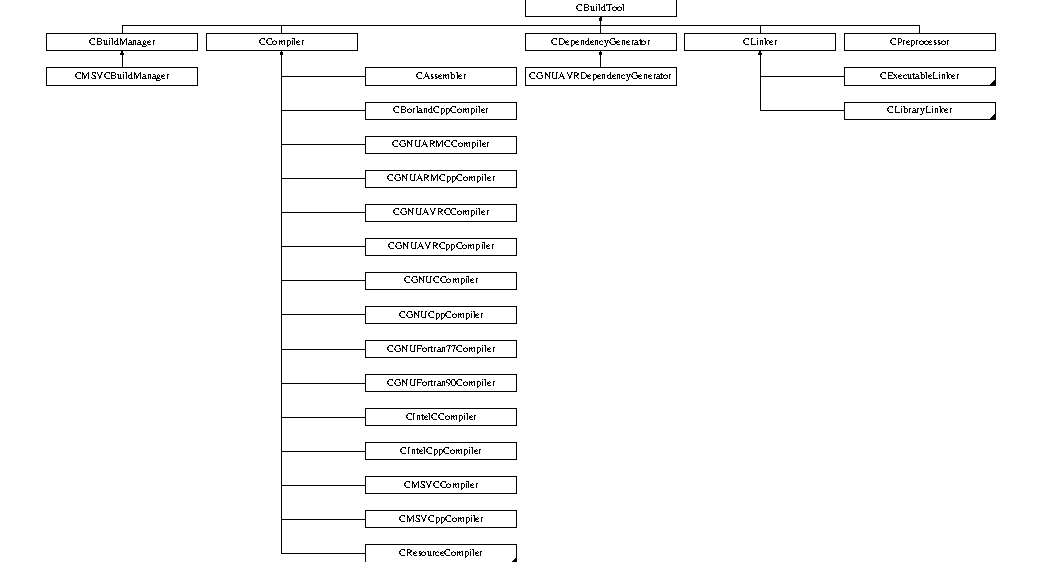
\includegraphics[height=7.555555cm]{d2/ddc/classCBuildTool}
\end{center}
\end{figure}
\subsection*{Public Types}
\begin{DoxyCompactItemize}
\item 
enum \hyperlink{classCBuildTool_a1a622843617ddf9b0ebb1c09c3437e6d}{Tool\-Type} \{ \\*
\hyperlink{classCBuildTool_a1a622843617ddf9b0ebb1c09c3437e6dab1bafc4d8b635a113d8aa8df402db376}{bt\-Other}, 
\hyperlink{classCBuildTool_a1a622843617ddf9b0ebb1c09c3437e6da682ffd4849664236bd9cea4ca37c9098}{bt\-Preprocessor}, 
\hyperlink{classCBuildTool_a1a622843617ddf9b0ebb1c09c3437e6dacea51ef0acdd86734df3fab58ab6ff63}{bt\-Assembler}, 
\hyperlink{classCBuildTool_a1a622843617ddf9b0ebb1c09c3437e6da6452f06a6962d6d1691764fc7547b2fa}{bt\-Compiler}, 
\\*
\hyperlink{classCBuildTool_a1a622843617ddf9b0ebb1c09c3437e6dafa84336de8da15476a3f18c592db84d8}{bt\-Resource\-Compiler}, 
\hyperlink{classCBuildTool_a1a622843617ddf9b0ebb1c09c3437e6daaa590d3915bffb1feeb7fabb95cfdcc9}{bt\-Static\-Linker}, 
\hyperlink{classCBuildTool_a1a622843617ddf9b0ebb1c09c3437e6da9337f68db623a79d23af60d99c31977f}{bt\-Dynamic\-Linker}, 
\hyperlink{classCBuildTool_a1a622843617ddf9b0ebb1c09c3437e6da304855adea8cd14d42cb204a8e0e412d}{bt\-Executable\-Linker}, 
\\*
\hyperlink{classCBuildTool_a1a622843617ddf9b0ebb1c09c3437e6dac9a46f3c5397fa8f045d5e302ae1ecdd}{bt\-Native\-Linker}, 
\hyperlink{classCBuildTool_a1a622843617ddf9b0ebb1c09c3437e6dae3a80faefcf67e0bd400b18640b59833}{bt\-Dependency\-Generator}, 
\hyperlink{classCBuildTool_a1a622843617ddf9b0ebb1c09c3437e6da3f42e0d5c99e78480c9955eb52c6a098}{bt\-Build\-Manager}, 
\hyperlink{classCBuildTool_a1a622843617ddf9b0ebb1c09c3437e6da7992e6bec75ea5848c159fdba11a5090}{bt\-Count}
 \}
\end{DoxyCompactItemize}
\subsection*{Public Member Functions}
\begin{DoxyCompactItemize}
\item 
\hyperlink{classCBuildTool_a1a622843617ddf9b0ebb1c09c3437e6d}{C\-Build\-Tool\-::\-Tool\-Type} \hyperlink{classCBuildTool_abd560ed1c839d6ff4c0be5a3d31c83fa}{Type} (void) const 
\item 
\hyperlink{classCString}{C\-String} \hyperlink{classCBuildTool_a8a78c520f210a52e89de6256ed2fd8af}{Type\-Name} (void) const 
\item 
\hyperlink{classCString}{C\-String} \& \hyperlink{classCBuildTool_a9f4bd07f77e0e5017fd437d4da7c9746}{Alias} (void)
\item 
\hyperlink{classCString}{C\-String} \& \hyperlink{classCBuildTool_a513c6a5dade6a3f397ca83dd32a6662b}{Description} (void)
\item 
\hyperlink{classCString}{C\-String} \& \hyperlink{classCBuildTool_a8405382b1f3b433ee55e879e74d65215}{Program} (void)
\item 
\hyperlink{classCString}{C\-String} \& \hyperlink{classCBuildTool_a971ed2f2b55d9f1127a218484b75aff6}{Make\-Variable} (void)
\item 
\hyperlink{classCString}{C\-String} \& \hyperlink{classCBuildTool_ab5238ad27196fd6d11650dd633c66284}{Command\-Template} (void)
\item 
\hyperlink{classCStringList}{C\-String\-List} \& \hyperlink{classCBuildTool_a6a764334cbcc2bf917237286938ad8fd}{Source\-Extensions} (void)
\item 
\hyperlink{classCString}{C\-String} \& \hyperlink{classCBuildTool_a3f957896383550c69d8f3136037b74bd}{Target\-Extension} (void)
\item 
bool \& \hyperlink{classCBuildTool_ab9e88543f1f7e2a760036ebff1c49298}{Need\-Quoted\-Path} (void)
\item 
bool \& \hyperlink{classCBuildTool_adae57be5c380f9e4e2a2934d7929816c}{Need\-Full\-Path} (void)
\item 
bool \& \hyperlink{classCBuildTool_a2b0f6b103a1d6de571da86a66a4853e7}{Need\-Unix\-Path} (void)
\item 
\hyperlink{classCString}{C\-String} \hyperlink{classCBuildTool_a21215cc9d80059ce00ed853b87e7d38d}{Make\-Command} (const \hyperlink{classCString}{C\-String} \&\hyperlink{classCBuildTool_ab5238ad27196fd6d11650dd633c66284}{Command\-Template}, \hyperlink{classCConfiguration}{C\-Configuration} \&Arguments)
\item 
\hyperlink{classCString}{C\-String} \hyperlink{classCBuildTool_a34da772ee708afd2f77e6222752ea2b4}{Make\-Command} (\hyperlink{classCConfiguration}{C\-Configuration} \&Arguments)
\item 
virtual bool \hyperlink{classCBuildTool_a34ad2894ff945f054ccd86db4007934f}{Expected\-Source\-Extension} (const \hyperlink{classCString}{C\-String} \&File\-Extension)
\item 
virtual \hyperlink{classCBuildTool}{C\-Build\-Tool} $\ast$ \hyperlink{classCBuildTool_aa7f0e7c0bd7f75c71d37df066bcb581e}{Create\-Instance} (void)
\item 
virtual void \hyperlink{classCBuildTool_ae36693eb03f822b8971a4e4b036111c2}{Clear} (void)
\item 
virtual void \hyperlink{classCBuildTool_abea21a0e61ab2177effdff5aaa169585}{Reset} (const \hyperlink{classCPlatform_a2fb735c63c53052f79629e338bb0f535}{C\-Platform\-::\-O\-S\-\_\-\-Type} O\-S)
\item 
virtual bool \hyperlink{classCBuildTool_ad07fcd46ccc841bc131d65505e5343c1}{Supports} (const \hyperlink{classCPlatform_a2fb735c63c53052f79629e338bb0f535}{C\-Platform\-::\-O\-S\-\_\-\-Type} O\-S)
\item 
virtual void \hyperlink{classCBuildTool_a299d87943c0f68dde5316318cc0838f8}{Read} (const Ti\-Xml\-Element $\ast$Build\-Tool\-Root)
\item 
virtual void \hyperlink{classCBuildTool_af0331a777785bc2d15236b5c74321ed2}{Write} (Ti\-Xml\-Element $\ast$Build\-Tool\-Root)
\item 
virtual void \hyperlink{classCBuildTool_a69815d1393a61dc16b2cc2d0552cd5ac}{Show} (void)
\item 
\hyperlink{classCBuildTool_a26f646e16e31257c97663d5651d60fdf}{C\-Build\-Tool} (void)
\item 
\hyperlink{classCBuildTool_aa4a2205a51b4c6b106f6218b63fd0f2d}{C\-Build\-Tool} (const \hyperlink{classCBuildTool}{C\-Build\-Tool} \&Build\-Tool)
\item 
virtual \hyperlink{classCBuildTool_a20a976c3fc44994a8f0a527869243409}{$\sim$\-C\-Build\-Tool} (void)
\end{DoxyCompactItemize}
\subsection*{Static Public Member Functions}
\begin{DoxyCompactItemize}
\item 
static \hyperlink{classCBuildTool_a1a622843617ddf9b0ebb1c09c3437e6d}{Tool\-Type} \hyperlink{classCBuildTool_a6ca8c98420c412d3e2cc78f11ef7f869}{Type} (const \hyperlink{classCString}{C\-String} \&Name)
\item 
static \hyperlink{classCString}{C\-String} \hyperlink{classCBuildTool_a14f8eedbb567cd410216a162b23a8d57}{Type\-Name} (const \hyperlink{classCBuildTool_a1a622843617ddf9b0ebb1c09c3437e6d}{Tool\-Type} \hyperlink{classCBuildTool_a6ca8c98420c412d3e2cc78f11ef7f869}{Type})
\item 
static \hyperlink{classCString}{C\-String} \hyperlink{classCBuildTool_a83ed37c5be4cdf13846ff4ae7ecca16c}{Abbrev\-Type\-Name} (const \hyperlink{classCBuildTool_a1a622843617ddf9b0ebb1c09c3437e6d}{Tool\-Type} \hyperlink{classCBuildTool_a6ca8c98420c412d3e2cc78f11ef7f869}{Type})
\end{DoxyCompactItemize}
\subsection*{Protected Member Functions}
\begin{DoxyCompactItemize}
\item 
void \hyperlink{classCBuildTool_a475f533bf444e533415138afa8ffb1fb}{Read} (const Ti\-Xml\-Element $\ast$Root, const \hyperlink{classCString}{C\-String} \&Name, \hyperlink{classCString}{C\-String} \&Value)
\item 
void \hyperlink{classCBuildTool_a16323a65679c6a29302aa6e9de178637}{Read} (const Ti\-Xml\-Element $\ast$Root, const \hyperlink{classCString}{C\-String} \&Name, bool \&Value)
\item 
void \hyperlink{classCBuildTool_a8c938967f1db9034c192c7a72de70054}{Write} (Ti\-Xml\-Element $\ast$Root, const \hyperlink{classCString}{C\-String} \&Name, const \hyperlink{classCString}{C\-String} \&Value)
\item 
void \hyperlink{classCBuildTool_af44193a557ad2df62c683fa5a2bd237b}{Write} (Ti\-Xml\-Element $\ast$Root, const \hyperlink{classCString}{C\-String} \&Name, const bool Value)
\end{DoxyCompactItemize}
\subsection*{Protected Attributes}
\begin{DoxyCompactItemize}
\item 
\hyperlink{classCPlatform_a2fb735c63c53052f79629e338bb0f535}{C\-Platform\-::\-O\-S\-\_\-\-Type} \hyperlink{classCBuildTool_ac71c95a56dbe26f62052dfff4f1c5c19}{m\-\_\-\-Platform}
\item 
\hyperlink{classCBuildTool_a1a622843617ddf9b0ebb1c09c3437e6d}{C\-Build\-Tool\-::\-Tool\-Type} \hyperlink{classCBuildTool_aca6ef29a8035174232c7b303ec5c51b1}{m\-\_\-\-Type}
\item 
\hyperlink{classCString}{C\-String} \hyperlink{classCBuildTool_a494ffa896b4101e77dda5f53954e0b71}{m\-\_\-\-Alias}
\item 
\hyperlink{classCString}{C\-String} \hyperlink{classCBuildTool_a366fc905a28c6b5d06f86830963fc2b7}{m\-\_\-\-Description}
\item 
\hyperlink{classCString}{C\-String} \hyperlink{classCBuildTool_af1a5473dde66a30d9aef8da074b8578f}{m\-\_\-\-Program}
\item 
\hyperlink{classCString}{C\-String} \hyperlink{classCBuildTool_a0dc54c7de4b25e7479bc8f025db697b7}{m\-\_\-\-Make\-Variable}
\item 
\hyperlink{classCString}{C\-String} \hyperlink{classCBuildTool_a2fa8d54915b30ee28de67d4928760967}{m\-\_\-\-Command\-Template}
\item 
\hyperlink{classCStringList}{C\-String\-List} \hyperlink{classCBuildTool_aca71945734de780a6b72f9aeb6e4a0c1}{m\-\_\-\-Source\-Extensions}
\item 
\hyperlink{classCString}{C\-String} \hyperlink{classCBuildTool_a358fae486209c5c9ee63d65e832bf815}{m\-\_\-\-Target\-Extension}
\item 
\hyperlink{classCString}{C\-String} \hyperlink{classCBuildTool_a7d7378e1398389dabb9e205c91a15c9b}{m\-\_\-\-Generic\-Switch}
\item 
bool \hyperlink{classCBuildTool_ad5ffb63aa12dc58c2305308e4f86486d}{m\-\_\-\-Need\-Quoted\-Path}
\item 
bool \hyperlink{classCBuildTool_ae4e23027052ad550bf8f0dbe04a96ae5}{m\-\_\-\-Need\-Full\-Path}
\item 
bool \hyperlink{classCBuildTool_a07c05a66337abb13b6c7cb3b577ac600}{m\-\_\-\-Need\-Unix\-Path}
\end{DoxyCompactItemize}


\subsection{Member Enumeration Documentation}
\hypertarget{classCBuildTool_a1a622843617ddf9b0ebb1c09c3437e6d}{\index{C\-Build\-Tool@{C\-Build\-Tool}!Tool\-Type@{Tool\-Type}}
\index{Tool\-Type@{Tool\-Type}!CBuildTool@{C\-Build\-Tool}}
\subsubsection[{Tool\-Type}]{\setlength{\rightskip}{0pt plus 5cm}enum {\bf C\-Build\-Tool\-::\-Tool\-Type}}}\label{classCBuildTool_a1a622843617ddf9b0ebb1c09c3437e6d}
\begin{Desc}
\item[Enumerator]\par
\begin{description}
\index{bt\-Other@{bt\-Other}!C\-Build\-Tool@{C\-Build\-Tool}}\index{C\-Build\-Tool@{C\-Build\-Tool}!bt\-Other@{bt\-Other}}\item[{\em 
\hypertarget{classCBuildTool_a1a622843617ddf9b0ebb1c09c3437e6dab1bafc4d8b635a113d8aa8df402db376}{bt\-Other}\label{classCBuildTool_a1a622843617ddf9b0ebb1c09c3437e6dab1bafc4d8b635a113d8aa8df402db376}
}]\index{bt\-Preprocessor@{bt\-Preprocessor}!C\-Build\-Tool@{C\-Build\-Tool}}\index{C\-Build\-Tool@{C\-Build\-Tool}!bt\-Preprocessor@{bt\-Preprocessor}}\item[{\em 
\hypertarget{classCBuildTool_a1a622843617ddf9b0ebb1c09c3437e6da682ffd4849664236bd9cea4ca37c9098}{bt\-Preprocessor}\label{classCBuildTool_a1a622843617ddf9b0ebb1c09c3437e6da682ffd4849664236bd9cea4ca37c9098}
}]\index{bt\-Assembler@{bt\-Assembler}!C\-Build\-Tool@{C\-Build\-Tool}}\index{C\-Build\-Tool@{C\-Build\-Tool}!bt\-Assembler@{bt\-Assembler}}\item[{\em 
\hypertarget{classCBuildTool_a1a622843617ddf9b0ebb1c09c3437e6dacea51ef0acdd86734df3fab58ab6ff63}{bt\-Assembler}\label{classCBuildTool_a1a622843617ddf9b0ebb1c09c3437e6dacea51ef0acdd86734df3fab58ab6ff63}
}]\index{bt\-Compiler@{bt\-Compiler}!C\-Build\-Tool@{C\-Build\-Tool}}\index{C\-Build\-Tool@{C\-Build\-Tool}!bt\-Compiler@{bt\-Compiler}}\item[{\em 
\hypertarget{classCBuildTool_a1a622843617ddf9b0ebb1c09c3437e6da6452f06a6962d6d1691764fc7547b2fa}{bt\-Compiler}\label{classCBuildTool_a1a622843617ddf9b0ebb1c09c3437e6da6452f06a6962d6d1691764fc7547b2fa}
}]\index{bt\-Resource\-Compiler@{bt\-Resource\-Compiler}!C\-Build\-Tool@{C\-Build\-Tool}}\index{C\-Build\-Tool@{C\-Build\-Tool}!bt\-Resource\-Compiler@{bt\-Resource\-Compiler}}\item[{\em 
\hypertarget{classCBuildTool_a1a622843617ddf9b0ebb1c09c3437e6dafa84336de8da15476a3f18c592db84d8}{bt\-Resource\-Compiler}\label{classCBuildTool_a1a622843617ddf9b0ebb1c09c3437e6dafa84336de8da15476a3f18c592db84d8}
}]\index{bt\-Static\-Linker@{bt\-Static\-Linker}!C\-Build\-Tool@{C\-Build\-Tool}}\index{C\-Build\-Tool@{C\-Build\-Tool}!bt\-Static\-Linker@{bt\-Static\-Linker}}\item[{\em 
\hypertarget{classCBuildTool_a1a622843617ddf9b0ebb1c09c3437e6daaa590d3915bffb1feeb7fabb95cfdcc9}{bt\-Static\-Linker}\label{classCBuildTool_a1a622843617ddf9b0ebb1c09c3437e6daaa590d3915bffb1feeb7fabb95cfdcc9}
}]\index{bt\-Dynamic\-Linker@{bt\-Dynamic\-Linker}!C\-Build\-Tool@{C\-Build\-Tool}}\index{C\-Build\-Tool@{C\-Build\-Tool}!bt\-Dynamic\-Linker@{bt\-Dynamic\-Linker}}\item[{\em 
\hypertarget{classCBuildTool_a1a622843617ddf9b0ebb1c09c3437e6da9337f68db623a79d23af60d99c31977f}{bt\-Dynamic\-Linker}\label{classCBuildTool_a1a622843617ddf9b0ebb1c09c3437e6da9337f68db623a79d23af60d99c31977f}
}]\index{bt\-Executable\-Linker@{bt\-Executable\-Linker}!C\-Build\-Tool@{C\-Build\-Tool}}\index{C\-Build\-Tool@{C\-Build\-Tool}!bt\-Executable\-Linker@{bt\-Executable\-Linker}}\item[{\em 
\hypertarget{classCBuildTool_a1a622843617ddf9b0ebb1c09c3437e6da304855adea8cd14d42cb204a8e0e412d}{bt\-Executable\-Linker}\label{classCBuildTool_a1a622843617ddf9b0ebb1c09c3437e6da304855adea8cd14d42cb204a8e0e412d}
}]\index{bt\-Native\-Linker@{bt\-Native\-Linker}!C\-Build\-Tool@{C\-Build\-Tool}}\index{C\-Build\-Tool@{C\-Build\-Tool}!bt\-Native\-Linker@{bt\-Native\-Linker}}\item[{\em 
\hypertarget{classCBuildTool_a1a622843617ddf9b0ebb1c09c3437e6dac9a46f3c5397fa8f045d5e302ae1ecdd}{bt\-Native\-Linker}\label{classCBuildTool_a1a622843617ddf9b0ebb1c09c3437e6dac9a46f3c5397fa8f045d5e302ae1ecdd}
}]\index{bt\-Dependency\-Generator@{bt\-Dependency\-Generator}!C\-Build\-Tool@{C\-Build\-Tool}}\index{C\-Build\-Tool@{C\-Build\-Tool}!bt\-Dependency\-Generator@{bt\-Dependency\-Generator}}\item[{\em 
\hypertarget{classCBuildTool_a1a622843617ddf9b0ebb1c09c3437e6dae3a80faefcf67e0bd400b18640b59833}{bt\-Dependency\-Generator}\label{classCBuildTool_a1a622843617ddf9b0ebb1c09c3437e6dae3a80faefcf67e0bd400b18640b59833}
}]\index{bt\-Build\-Manager@{bt\-Build\-Manager}!C\-Build\-Tool@{C\-Build\-Tool}}\index{C\-Build\-Tool@{C\-Build\-Tool}!bt\-Build\-Manager@{bt\-Build\-Manager}}\item[{\em 
\hypertarget{classCBuildTool_a1a622843617ddf9b0ebb1c09c3437e6da3f42e0d5c99e78480c9955eb52c6a098}{bt\-Build\-Manager}\label{classCBuildTool_a1a622843617ddf9b0ebb1c09c3437e6da3f42e0d5c99e78480c9955eb52c6a098}
}]\index{bt\-Count@{bt\-Count}!C\-Build\-Tool@{C\-Build\-Tool}}\index{C\-Build\-Tool@{C\-Build\-Tool}!bt\-Count@{bt\-Count}}\item[{\em 
\hypertarget{classCBuildTool_a1a622843617ddf9b0ebb1c09c3437e6da7992e6bec75ea5848c159fdba11a5090}{bt\-Count}\label{classCBuildTool_a1a622843617ddf9b0ebb1c09c3437e6da7992e6bec75ea5848c159fdba11a5090}
}]\end{description}
\end{Desc}


\subsection{Constructor \& Destructor Documentation}
\hypertarget{classCBuildTool_a26f646e16e31257c97663d5651d60fdf}{\index{C\-Build\-Tool@{C\-Build\-Tool}!C\-Build\-Tool@{C\-Build\-Tool}}
\index{C\-Build\-Tool@{C\-Build\-Tool}!CBuildTool@{C\-Build\-Tool}}
\subsubsection[{C\-Build\-Tool}]{\setlength{\rightskip}{0pt plus 5cm}C\-Build\-Tool\-::\-C\-Build\-Tool (
\begin{DoxyParamCaption}
\item[{void}]{}
\end{DoxyParamCaption}
)}}\label{classCBuildTool_a26f646e16e31257c97663d5651d60fdf}
\hypertarget{classCBuildTool_aa4a2205a51b4c6b106f6218b63fd0f2d}{\index{C\-Build\-Tool@{C\-Build\-Tool}!C\-Build\-Tool@{C\-Build\-Tool}}
\index{C\-Build\-Tool@{C\-Build\-Tool}!CBuildTool@{C\-Build\-Tool}}
\subsubsection[{C\-Build\-Tool}]{\setlength{\rightskip}{0pt plus 5cm}C\-Build\-Tool\-::\-C\-Build\-Tool (
\begin{DoxyParamCaption}
\item[{const {\bf C\-Build\-Tool} \&}]{Build\-Tool}
\end{DoxyParamCaption}
)}}\label{classCBuildTool_aa4a2205a51b4c6b106f6218b63fd0f2d}
\hypertarget{classCBuildTool_a20a976c3fc44994a8f0a527869243409}{\index{C\-Build\-Tool@{C\-Build\-Tool}!$\sim$\-C\-Build\-Tool@{$\sim$\-C\-Build\-Tool}}
\index{$\sim$\-C\-Build\-Tool@{$\sim$\-C\-Build\-Tool}!CBuildTool@{C\-Build\-Tool}}
\subsubsection[{$\sim$\-C\-Build\-Tool}]{\setlength{\rightskip}{0pt plus 5cm}C\-Build\-Tool\-::$\sim$\-C\-Build\-Tool (
\begin{DoxyParamCaption}
\item[{void}]{}
\end{DoxyParamCaption}
)\hspace{0.3cm}{\ttfamily [virtual]}}}\label{classCBuildTool_a20a976c3fc44994a8f0a527869243409}


\subsection{Member Function Documentation}
\hypertarget{classCBuildTool_a83ed37c5be4cdf13846ff4ae7ecca16c}{\index{C\-Build\-Tool@{C\-Build\-Tool}!Abbrev\-Type\-Name@{Abbrev\-Type\-Name}}
\index{Abbrev\-Type\-Name@{Abbrev\-Type\-Name}!CBuildTool@{C\-Build\-Tool}}
\subsubsection[{Abbrev\-Type\-Name}]{\setlength{\rightskip}{0pt plus 5cm}{\bf C\-String} C\-Build\-Tool\-::\-Abbrev\-Type\-Name (
\begin{DoxyParamCaption}
\item[{const {\bf Tool\-Type}}]{Type}
\end{DoxyParamCaption}
)\hspace{0.3cm}{\ttfamily [static]}}}\label{classCBuildTool_a83ed37c5be4cdf13846ff4ae7ecca16c}
\hypertarget{classCBuildTool_a9f4bd07f77e0e5017fd437d4da7c9746}{\index{C\-Build\-Tool@{C\-Build\-Tool}!Alias@{Alias}}
\index{Alias@{Alias}!CBuildTool@{C\-Build\-Tool}}
\subsubsection[{Alias}]{\setlength{\rightskip}{0pt plus 5cm}{\bf C\-String}\& C\-Build\-Tool\-::\-Alias (
\begin{DoxyParamCaption}
\item[{void}]{}
\end{DoxyParamCaption}
)\hspace{0.3cm}{\ttfamily [inline]}}}\label{classCBuildTool_a9f4bd07f77e0e5017fd437d4da7c9746}
\hypertarget{classCBuildTool_ae36693eb03f822b8971a4e4b036111c2}{\index{C\-Build\-Tool@{C\-Build\-Tool}!Clear@{Clear}}
\index{Clear@{Clear}!CBuildTool@{C\-Build\-Tool}}
\subsubsection[{Clear}]{\setlength{\rightskip}{0pt plus 5cm}void C\-Build\-Tool\-::\-Clear (
\begin{DoxyParamCaption}
\item[{void}]{}
\end{DoxyParamCaption}
)\hspace{0.3cm}{\ttfamily [virtual]}}}\label{classCBuildTool_ae36693eb03f822b8971a4e4b036111c2}
\hypertarget{classCBuildTool_ab5238ad27196fd6d11650dd633c66284}{\index{C\-Build\-Tool@{C\-Build\-Tool}!Command\-Template@{Command\-Template}}
\index{Command\-Template@{Command\-Template}!CBuildTool@{C\-Build\-Tool}}
\subsubsection[{Command\-Template}]{\setlength{\rightskip}{0pt plus 5cm}{\bf C\-String}\& C\-Build\-Tool\-::\-Command\-Template (
\begin{DoxyParamCaption}
\item[{void}]{}
\end{DoxyParamCaption}
)\hspace{0.3cm}{\ttfamily [inline]}}}\label{classCBuildTool_ab5238ad27196fd6d11650dd633c66284}
\hypertarget{classCBuildTool_aa7f0e7c0bd7f75c71d37df066bcb581e}{\index{C\-Build\-Tool@{C\-Build\-Tool}!Create\-Instance@{Create\-Instance}}
\index{Create\-Instance@{Create\-Instance}!CBuildTool@{C\-Build\-Tool}}
\subsubsection[{Create\-Instance}]{\setlength{\rightskip}{0pt plus 5cm}{\bf C\-Build\-Tool} $\ast$ C\-Build\-Tool\-::\-Create\-Instance (
\begin{DoxyParamCaption}
\item[{void}]{}
\end{DoxyParamCaption}
)\hspace{0.3cm}{\ttfamily [virtual]}}}\label{classCBuildTool_aa7f0e7c0bd7f75c71d37df066bcb581e}


Reimplemented in \hyperlink{classCMSVCBuildManager_a2519f0cd2477b6f9bd4459b15635c466}{C\-M\-S\-V\-C\-Build\-Manager}, \hyperlink{classCMSVCNativeExecutableLinker_ab769242f54c4336e1cedd340b8a45d3a}{C\-M\-S\-V\-C\-Native\-Executable\-Linker}, \hyperlink{classCMSVCConsoleExecutableLinker_a9240460d8f7ea9651177279bf0640a88}{C\-M\-S\-V\-C\-Console\-Executable\-Linker}, \hyperlink{classCMSVCExecutableLinker_ad5b1391fa863f9e966562ee227a00693}{C\-M\-S\-V\-C\-Executable\-Linker}, \hyperlink{classCMSVCDynamicLinker_ad8fc45d290987fb96b9a983b592a2ad1}{C\-M\-S\-V\-C\-Dynamic\-Linker}, \hyperlink{classCMSVCStaticLinker_ab05784f22189ba02f8d2f4be2c3ab095}{C\-M\-S\-V\-C\-Static\-Linker}, \hyperlink{classCMSVCResourceCompiler_aabd1683b76c181322754107af65ed8e0}{C\-M\-S\-V\-C\-Resource\-Compiler}, \hyperlink{classCMSVCppCompiler_ace8c0f315b83286474cdf8c8b41db75a}{C\-M\-S\-V\-Cpp\-Compiler}, \hyperlink{classCMSVCCompiler_a00dec77c231cace2f66fe45fccb25c7e}{C\-M\-S\-V\-C\-Compiler}, \hyperlink{classCIntelExecutableLinker_aacec1bc57c88a614c449a6873c1cc489}{C\-Intel\-Executable\-Linker}, \hyperlink{classCIntelDynamicLinker_a51e4c22985b5c518e8cdef1abeee7d85}{C\-Intel\-Dynamic\-Linker}, \hyperlink{classCIntelStaticLinker_af5e68a1b09bc64dd30af6d7e9ffe6266}{C\-Intel\-Static\-Linker}, \hyperlink{classCIntelCppCompiler_a2e75b0ac5a7860128f25f29698f51509}{C\-Intel\-Cpp\-Compiler}, \hyperlink{classCIntelCCompiler_a4f259da4011feabc53b1ebf9a26bd2de}{C\-Intel\-C\-Compiler}, \hyperlink{classCBorlandConsoleExecutableLinker_a1aba394784a724a2b59c021b732484f8}{C\-Borland\-Console\-Executable\-Linker}, \hyperlink{classCBorlandExecutableLinker_ab4acecd477ed0458760a3f14ee6fb868}{C\-Borland\-Executable\-Linker}, \hyperlink{classCBorlandDynamicLinker_ae76cbd521d03bd3eee2f1d5fe8836d03}{C\-Borland\-Dynamic\-Linker}, \hyperlink{classCBorlandStaticLinker_ac5c637b9e4762cf272d8710be8212857}{C\-Borland\-Static\-Linker}, \hyperlink{classCBorlandResourceCompiler_a5c6aeef4fa07fb9693feb860a70729e0}{C\-Borland\-Resource\-Compiler}, \hyperlink{classCBorlandCppCompiler_a49178aa21245a1400f38c71631b7fa78}{C\-Borland\-Cpp\-Compiler}, \hyperlink{classCGNUARMExecutableLinker_a9241ead8113a3c4c3820240f3993fb19}{C\-G\-N\-U\-A\-R\-M\-Executable\-Linker}, \hyperlink{classCGNUARMDynamicLinker_ad3ded52b8101b6f85ad6d5609f85c78c}{C\-G\-N\-U\-A\-R\-M\-Dynamic\-Linker}, \hyperlink{classCGNUARMStaticLinker_a7cac8fed64437b826d085b0cf33aeaf8}{C\-G\-N\-U\-A\-R\-M\-Static\-Linker}, \hyperlink{classCGNUARMWindowsResourceCompiler_a8da0eff0b561e69f2e2178965cd69253}{C\-G\-N\-U\-A\-R\-M\-Windows\-Resource\-Compiler}, \hyperlink{classCGNUARMCppCompiler_ae61a4db30f31a36bc46341da83ac9c63}{C\-G\-N\-U\-A\-R\-M\-Cpp\-Compiler}, \hyperlink{classCGNUARMCCompiler_a3e102dcc65d172a098282c5554e79302}{C\-G\-N\-U\-A\-R\-M\-C\-Compiler}, \hyperlink{classCGNUAVRDependencyGenerator_a5d4d5e45d1cdd58d998ac961a66647dc}{C\-G\-N\-U\-A\-V\-R\-Dependency\-Generator}, \hyperlink{classCGNUAVRExecutableLinker_ad6c7693277ecb00d550bde8e1bda0b8c}{C\-G\-N\-U\-A\-V\-R\-Executable\-Linker}, \hyperlink{classCGNUAVRDynamicLinker_ae26802d4ce8ce7c45a87a65bf7066832}{C\-G\-N\-U\-A\-V\-R\-Dynamic\-Linker}, \hyperlink{classCGNUAVRStaticLinker_ad4852b66cb610455765089ff8fdb7771}{C\-G\-N\-U\-A\-V\-R\-Static\-Linker}, \hyperlink{classCGNUAVRCppCompiler_ac38cdc207e9dce42f53fef90ebaa3b87}{C\-G\-N\-U\-A\-V\-R\-Cpp\-Compiler}, \hyperlink{classCGNUAVRCCompiler_ad5630a463e0a41b5ecf28295f2c16e2f}{C\-G\-N\-U\-A\-V\-R\-C\-Compiler}, \hyperlink{classCGNUExecutableLinker_a96d5c82ab5c7c26e7e9ef1542c815e94}{C\-G\-N\-U\-Executable\-Linker}, \hyperlink{classCGNUDynamicLinker_addcaa2506e1f804b4737cb564a899f6c}{C\-G\-N\-U\-Dynamic\-Linker}, \hyperlink{classCGNUStaticLinker_aa2e18f13e37d6c4fe3016d55bc67f746}{C\-G\-N\-U\-Static\-Linker}, \hyperlink{classCGNUWindowsResourceCompiler_a295b322f12aa797537c0ef38bed0a9a5}{C\-G\-N\-U\-Windows\-Resource\-Compiler}, \hyperlink{classCGNUFortran90Compiler_a40bbc9c4d1417331e65990ed6f402d24}{C\-G\-N\-U\-Fortran90\-Compiler}, \hyperlink{classCGNUFortran77Compiler_ac9303b9366e63a08983cabcdfcb5cf06}{C\-G\-N\-U\-Fortran77\-Compiler}, \hyperlink{classCGNUCppCompiler_a0e6856b3906b6b32951f9796fba16316}{C\-G\-N\-U\-Cpp\-Compiler}, \hyperlink{classCGNUCCompiler_ae69827132a9bc1170f2073bf4ded88bc}{C\-G\-N\-U\-C\-Compiler}, \hyperlink{classCBuildManager_a3613cf27c028cb883a5b309a8c024d75}{C\-Build\-Manager}, \hyperlink{classCDependencyGenerator_af25a1710b95578b0e7ebcec02c4a7238}{C\-Dependency\-Generator}, \hyperlink{classCExecutableLinker_a457b823b737b0a78285d5ede77df827c}{C\-Executable\-Linker}, \hyperlink{classCDynamicLinker_ac71406ca5c6e8e991a6418a6307d274c}{C\-Dynamic\-Linker}, \hyperlink{classCStaticLinker_a7e626491caa847ef207032ee600625db}{C\-Static\-Linker}, \hyperlink{classCLibraryLinker_a02b85c6bc81ad2973ee9a578412a1fa0}{C\-Library\-Linker}, \hyperlink{classCLinker_a9b644b9c906436f75b394f2324d811d3}{C\-Linker}, \hyperlink{classCResourceCompiler_a4f46ae1558a0096b040eb593d28a810c}{C\-Resource\-Compiler}, \hyperlink{classCAssembler_abc4ab373b93fc0980c204764afa73306}{C\-Assembler}, \hyperlink{classCCompiler_a3d4aaaf69e1ba6070c729fd042d90012}{C\-Compiler}, and \hyperlink{classCPreprocessor_af3308b7a4153f39320345f12f3da231c}{C\-Preprocessor}.

\hypertarget{classCBuildTool_a513c6a5dade6a3f397ca83dd32a6662b}{\index{C\-Build\-Tool@{C\-Build\-Tool}!Description@{Description}}
\index{Description@{Description}!CBuildTool@{C\-Build\-Tool}}
\subsubsection[{Description}]{\setlength{\rightskip}{0pt plus 5cm}{\bf C\-String}\& C\-Build\-Tool\-::\-Description (
\begin{DoxyParamCaption}
\item[{void}]{}
\end{DoxyParamCaption}
)\hspace{0.3cm}{\ttfamily [inline]}}}\label{classCBuildTool_a513c6a5dade6a3f397ca83dd32a6662b}
\hypertarget{classCBuildTool_a34ad2894ff945f054ccd86db4007934f}{\index{C\-Build\-Tool@{C\-Build\-Tool}!Expected\-Source\-Extension@{Expected\-Source\-Extension}}
\index{Expected\-Source\-Extension@{Expected\-Source\-Extension}!CBuildTool@{C\-Build\-Tool}}
\subsubsection[{Expected\-Source\-Extension}]{\setlength{\rightskip}{0pt plus 5cm}bool C\-Build\-Tool\-::\-Expected\-Source\-Extension (
\begin{DoxyParamCaption}
\item[{const {\bf C\-String} \&}]{File\-Extension}
\end{DoxyParamCaption}
)\hspace{0.3cm}{\ttfamily [virtual]}}}\label{classCBuildTool_a34ad2894ff945f054ccd86db4007934f}
\hypertarget{classCBuildTool_a21215cc9d80059ce00ed853b87e7d38d}{\index{C\-Build\-Tool@{C\-Build\-Tool}!Make\-Command@{Make\-Command}}
\index{Make\-Command@{Make\-Command}!CBuildTool@{C\-Build\-Tool}}
\subsubsection[{Make\-Command}]{\setlength{\rightskip}{0pt plus 5cm}{\bf C\-String} C\-Build\-Tool\-::\-Make\-Command (
\begin{DoxyParamCaption}
\item[{const {\bf C\-String} \&}]{Command\-Template, }
\item[{{\bf C\-Configuration} \&}]{Arguments}
\end{DoxyParamCaption}
)}}\label{classCBuildTool_a21215cc9d80059ce00ed853b87e7d38d}
\hypertarget{classCBuildTool_a34da772ee708afd2f77e6222752ea2b4}{\index{C\-Build\-Tool@{C\-Build\-Tool}!Make\-Command@{Make\-Command}}
\index{Make\-Command@{Make\-Command}!CBuildTool@{C\-Build\-Tool}}
\subsubsection[{Make\-Command}]{\setlength{\rightskip}{0pt plus 5cm}{\bf C\-String} C\-Build\-Tool\-::\-Make\-Command (
\begin{DoxyParamCaption}
\item[{{\bf C\-Configuration} \&}]{Arguments}
\end{DoxyParamCaption}
)}}\label{classCBuildTool_a34da772ee708afd2f77e6222752ea2b4}
\hypertarget{classCBuildTool_a971ed2f2b55d9f1127a218484b75aff6}{\index{C\-Build\-Tool@{C\-Build\-Tool}!Make\-Variable@{Make\-Variable}}
\index{Make\-Variable@{Make\-Variable}!CBuildTool@{C\-Build\-Tool}}
\subsubsection[{Make\-Variable}]{\setlength{\rightskip}{0pt plus 5cm}{\bf C\-String}\& C\-Build\-Tool\-::\-Make\-Variable (
\begin{DoxyParamCaption}
\item[{void}]{}
\end{DoxyParamCaption}
)\hspace{0.3cm}{\ttfamily [inline]}}}\label{classCBuildTool_a971ed2f2b55d9f1127a218484b75aff6}
\hypertarget{classCBuildTool_adae57be5c380f9e4e2a2934d7929816c}{\index{C\-Build\-Tool@{C\-Build\-Tool}!Need\-Full\-Path@{Need\-Full\-Path}}
\index{Need\-Full\-Path@{Need\-Full\-Path}!CBuildTool@{C\-Build\-Tool}}
\subsubsection[{Need\-Full\-Path}]{\setlength{\rightskip}{0pt plus 5cm}bool\& C\-Build\-Tool\-::\-Need\-Full\-Path (
\begin{DoxyParamCaption}
\item[{void}]{}
\end{DoxyParamCaption}
)\hspace{0.3cm}{\ttfamily [inline]}}}\label{classCBuildTool_adae57be5c380f9e4e2a2934d7929816c}
\hypertarget{classCBuildTool_ab9e88543f1f7e2a760036ebff1c49298}{\index{C\-Build\-Tool@{C\-Build\-Tool}!Need\-Quoted\-Path@{Need\-Quoted\-Path}}
\index{Need\-Quoted\-Path@{Need\-Quoted\-Path}!CBuildTool@{C\-Build\-Tool}}
\subsubsection[{Need\-Quoted\-Path}]{\setlength{\rightskip}{0pt plus 5cm}bool\& C\-Build\-Tool\-::\-Need\-Quoted\-Path (
\begin{DoxyParamCaption}
\item[{void}]{}
\end{DoxyParamCaption}
)\hspace{0.3cm}{\ttfamily [inline]}}}\label{classCBuildTool_ab9e88543f1f7e2a760036ebff1c49298}
\hypertarget{classCBuildTool_a2b0f6b103a1d6de571da86a66a4853e7}{\index{C\-Build\-Tool@{C\-Build\-Tool}!Need\-Unix\-Path@{Need\-Unix\-Path}}
\index{Need\-Unix\-Path@{Need\-Unix\-Path}!CBuildTool@{C\-Build\-Tool}}
\subsubsection[{Need\-Unix\-Path}]{\setlength{\rightskip}{0pt plus 5cm}bool\& C\-Build\-Tool\-::\-Need\-Unix\-Path (
\begin{DoxyParamCaption}
\item[{void}]{}
\end{DoxyParamCaption}
)\hspace{0.3cm}{\ttfamily [inline]}}}\label{classCBuildTool_a2b0f6b103a1d6de571da86a66a4853e7}
\hypertarget{classCBuildTool_a8405382b1f3b433ee55e879e74d65215}{\index{C\-Build\-Tool@{C\-Build\-Tool}!Program@{Program}}
\index{Program@{Program}!CBuildTool@{C\-Build\-Tool}}
\subsubsection[{Program}]{\setlength{\rightskip}{0pt plus 5cm}{\bf C\-String}\& C\-Build\-Tool\-::\-Program (
\begin{DoxyParamCaption}
\item[{void}]{}
\end{DoxyParamCaption}
)\hspace{0.3cm}{\ttfamily [inline]}}}\label{classCBuildTool_a8405382b1f3b433ee55e879e74d65215}
\hypertarget{classCBuildTool_a475f533bf444e533415138afa8ffb1fb}{\index{C\-Build\-Tool@{C\-Build\-Tool}!Read@{Read}}
\index{Read@{Read}!CBuildTool@{C\-Build\-Tool}}
\subsubsection[{Read}]{\setlength{\rightskip}{0pt plus 5cm}void C\-Build\-Tool\-::\-Read (
\begin{DoxyParamCaption}
\item[{const Ti\-Xml\-Element $\ast$}]{Root, }
\item[{const {\bf C\-String} \&}]{Name, }
\item[{{\bf C\-String} \&}]{Value}
\end{DoxyParamCaption}
)\hspace{0.3cm}{\ttfamily [protected]}}}\label{classCBuildTool_a475f533bf444e533415138afa8ffb1fb}
\hypertarget{classCBuildTool_a16323a65679c6a29302aa6e9de178637}{\index{C\-Build\-Tool@{C\-Build\-Tool}!Read@{Read}}
\index{Read@{Read}!CBuildTool@{C\-Build\-Tool}}
\subsubsection[{Read}]{\setlength{\rightskip}{0pt plus 5cm}void C\-Build\-Tool\-::\-Read (
\begin{DoxyParamCaption}
\item[{const Ti\-Xml\-Element $\ast$}]{Root, }
\item[{const {\bf C\-String} \&}]{Name, }
\item[{bool \&}]{Value}
\end{DoxyParamCaption}
)\hspace{0.3cm}{\ttfamily [protected]}}}\label{classCBuildTool_a16323a65679c6a29302aa6e9de178637}
\hypertarget{classCBuildTool_a299d87943c0f68dde5316318cc0838f8}{\index{C\-Build\-Tool@{C\-Build\-Tool}!Read@{Read}}
\index{Read@{Read}!CBuildTool@{C\-Build\-Tool}}
\subsubsection[{Read}]{\setlength{\rightskip}{0pt plus 5cm}void C\-Build\-Tool\-::\-Read (
\begin{DoxyParamCaption}
\item[{const Ti\-Xml\-Element $\ast$}]{Build\-Tool\-Root}
\end{DoxyParamCaption}
)\hspace{0.3cm}{\ttfamily [virtual]}}}\label{classCBuildTool_a299d87943c0f68dde5316318cc0838f8}


Reimplemented in \hyperlink{classCBuildManager_a3a2dfa7800c44b7122a248d32dffe193}{C\-Build\-Manager}, \hyperlink{classCDependencyGenerator_aaaff3838bea1e65ba250b78f1746870c}{C\-Dependency\-Generator}, \hyperlink{classCExecutableLinker_a181ea374618a85985db14f468dc63023}{C\-Executable\-Linker}, \hyperlink{classCLinker_a6db5ff1a933b56855b2bfb9260f46dce}{C\-Linker}, \hyperlink{classCCompiler_ac842b165479db817bb86d56367988b10}{C\-Compiler}, and \hyperlink{classCPreprocessor_a30e3222f8d535865ef691d922ec4615e}{C\-Preprocessor}.

\hypertarget{classCBuildTool_abea21a0e61ab2177effdff5aaa169585}{\index{C\-Build\-Tool@{C\-Build\-Tool}!Reset@{Reset}}
\index{Reset@{Reset}!CBuildTool@{C\-Build\-Tool}}
\subsubsection[{Reset}]{\setlength{\rightskip}{0pt plus 5cm}void C\-Build\-Tool\-::\-Reset (
\begin{DoxyParamCaption}
\item[{const {\bf C\-Platform\-::\-O\-S\-\_\-\-Type}}]{O\-S}
\end{DoxyParamCaption}
)\hspace{0.3cm}{\ttfamily [virtual]}}}\label{classCBuildTool_abea21a0e61ab2177effdff5aaa169585}


Reimplemented in \hyperlink{classCMSVCBuildManager_a1ca4f16c93948c195a65d14746555bea}{C\-M\-S\-V\-C\-Build\-Manager}, \hyperlink{classCMSVCNativeExecutableLinker_ab3fb3e7311543adbb49e2ea4d1e1070d}{C\-M\-S\-V\-C\-Native\-Executable\-Linker}, \hyperlink{classCMSVCConsoleExecutableLinker_a79315457d3dfc639a33e60426a67e956}{C\-M\-S\-V\-C\-Console\-Executable\-Linker}, \hyperlink{classCMSVCExecutableLinker_aec2b90e8609888c052952a2072d65f52}{C\-M\-S\-V\-C\-Executable\-Linker}, \hyperlink{classCMSVCDynamicLinker_aae22160e1bee1d4231ce669ac0132937}{C\-M\-S\-V\-C\-Dynamic\-Linker}, \hyperlink{classCMSVCStaticLinker_ac7a93fa46130ad965232df605574a41c}{C\-M\-S\-V\-C\-Static\-Linker}, \hyperlink{classCMSVCResourceCompiler_a0e48cbff3bc0d94803c0b2307317f05b}{C\-M\-S\-V\-C\-Resource\-Compiler}, \hyperlink{classCMSVCppCompiler_ac159b7332272495733a159641a1e6274}{C\-M\-S\-V\-Cpp\-Compiler}, \hyperlink{classCMSVCCompiler_add080abc4d9d62ecfb08d0acb32b7693}{C\-M\-S\-V\-C\-Compiler}, \hyperlink{classCIntelExecutableLinker_adb14460fc50fb8d0e7ef29fd991d4271}{C\-Intel\-Executable\-Linker}, \hyperlink{classCIntelDynamicLinker_a9716e2053535fcadd92d46699d8b445e}{C\-Intel\-Dynamic\-Linker}, \hyperlink{classCIntelStaticLinker_a71064c1a78086c73ddae37f4ecf513c2}{C\-Intel\-Static\-Linker}, \hyperlink{classCIntelCppCompiler_a39338f5aead731a4fc834605d2d60c37}{C\-Intel\-Cpp\-Compiler}, \hyperlink{classCIntelCCompiler_af5d140834df595d4b5e370e534acb933}{C\-Intel\-C\-Compiler}, \hyperlink{classCBorlandConsoleExecutableLinker_a0b31e3b17b2c03a4d6d6ada4fe8b48e0}{C\-Borland\-Console\-Executable\-Linker}, \hyperlink{classCBorlandExecutableLinker_a90ea600853600bac560530248a4a82b4}{C\-Borland\-Executable\-Linker}, \hyperlink{classCBorlandDynamicLinker_acbf22349e7e89873dac5f55f8d9adc8b}{C\-Borland\-Dynamic\-Linker}, \hyperlink{classCBorlandStaticLinker_a179338b382e0a92ccc927666c52cdf18}{C\-Borland\-Static\-Linker}, \hyperlink{classCBorlandResourceCompiler_a586f49a9ccb4b38f3a74534eb3876c55}{C\-Borland\-Resource\-Compiler}, \hyperlink{classCBorlandCppCompiler_ac329f9e685bd1a702d7545fa991be71d}{C\-Borland\-Cpp\-Compiler}, \hyperlink{classCGNUARMExecutableLinker_a9c3143f13605d317022dca24f134ff39}{C\-G\-N\-U\-A\-R\-M\-Executable\-Linker}, \hyperlink{classCGNUARMDynamicLinker_a3f49a2938f97c58d9eaee0986f3b9866}{C\-G\-N\-U\-A\-R\-M\-Dynamic\-Linker}, \hyperlink{classCGNUARMStaticLinker_a2bb9852d9ddd5ad71fdd2bb9a374343e}{C\-G\-N\-U\-A\-R\-M\-Static\-Linker}, \hyperlink{classCGNUARMWindowsResourceCompiler_a0eae18d396f5bfc5ffcd76af42b8d093}{C\-G\-N\-U\-A\-R\-M\-Windows\-Resource\-Compiler}, \hyperlink{classCGNUARMCppCompiler_aa51e81dcb2d4a6982aae3c8627e3fdc6}{C\-G\-N\-U\-A\-R\-M\-Cpp\-Compiler}, \hyperlink{classCGNUARMCCompiler_a379674393ab735aae49e718d8da8d71a}{C\-G\-N\-U\-A\-R\-M\-C\-Compiler}, \hyperlink{classCGNUAVRDependencyGenerator_af96f3eb85393be62b8b91f0376b17273}{C\-G\-N\-U\-A\-V\-R\-Dependency\-Generator}, \hyperlink{classCGNUAVRExecutableLinker_a2bb4fb92e5d0d6846a8635e1ebcc9ccb}{C\-G\-N\-U\-A\-V\-R\-Executable\-Linker}, \hyperlink{classCGNUAVRDynamicLinker_a08c53dfc9f1352a486bfb736aee544f4}{C\-G\-N\-U\-A\-V\-R\-Dynamic\-Linker}, \hyperlink{classCGNUAVRStaticLinker_aed827fdf1de17dfdbcdfe0ba4ca55fda}{C\-G\-N\-U\-A\-V\-R\-Static\-Linker}, \hyperlink{classCGNUAVRCppCompiler_a3c597b2862b70725bcbc2d518c90f7bd}{C\-G\-N\-U\-A\-V\-R\-Cpp\-Compiler}, \hyperlink{classCGNUAVRCCompiler_a7f1f5abcd42d933e732c33bae1e18763}{C\-G\-N\-U\-A\-V\-R\-C\-Compiler}, \hyperlink{classCGNUExecutableLinker_a79d1592b592c3b48d7e1683cdb516d85}{C\-G\-N\-U\-Executable\-Linker}, \hyperlink{classCGNUDynamicLinker_ae156df1627238831556bd40597694d7e}{C\-G\-N\-U\-Dynamic\-Linker}, \hyperlink{classCGNUStaticLinker_a12dca4d9b21cac925906776310521240}{C\-G\-N\-U\-Static\-Linker}, \hyperlink{classCGNUWindowsResourceCompiler_add9c139a642cf1d18a3fb2978bb792c4}{C\-G\-N\-U\-Windows\-Resource\-Compiler}, \hyperlink{classCGNUFortran90Compiler_a6ab744c56fb1f147587fee587d15b652}{C\-G\-N\-U\-Fortran90\-Compiler}, \hyperlink{classCGNUFortran77Compiler_a67867de4d567f8afc4758083b29be23a}{C\-G\-N\-U\-Fortran77\-Compiler}, \hyperlink{classCGNUCppCompiler_ae44ff252152bc51ef1855cc863cb007b}{C\-G\-N\-U\-Cpp\-Compiler}, \hyperlink{classCGNUCCompiler_a56fec9a27346838f33b3c444e90021f7}{C\-G\-N\-U\-C\-Compiler}, and \hyperlink{classCDynamicLinker_a437d46ee65b3585e7be9d15d40c26820}{C\-Dynamic\-Linker}.

\hypertarget{classCBuildTool_a69815d1393a61dc16b2cc2d0552cd5ac}{\index{C\-Build\-Tool@{C\-Build\-Tool}!Show@{Show}}
\index{Show@{Show}!CBuildTool@{C\-Build\-Tool}}
\subsubsection[{Show}]{\setlength{\rightskip}{0pt plus 5cm}void C\-Build\-Tool\-::\-Show (
\begin{DoxyParamCaption}
\item[{void}]{}
\end{DoxyParamCaption}
)\hspace{0.3cm}{\ttfamily [virtual]}}}\label{classCBuildTool_a69815d1393a61dc16b2cc2d0552cd5ac}


Reimplemented in \hyperlink{classCBuildManager_a6a7e968c30cef765316d06a1f0a6d76c}{C\-Build\-Manager}, \hyperlink{classCDependencyGenerator_a632c6eedf0b8d948748fb29f47545451}{C\-Dependency\-Generator}, \hyperlink{classCExecutableLinker_a01fa91b454c4cc4d154a26f0ab8da467}{C\-Executable\-Linker}, \hyperlink{classCLinker_aa2c99f02f4433dfae7cdc0654b901582}{C\-Linker}, \hyperlink{classCCompiler_a07a1bbfb0fc606cf74bccc1ab64a64e8}{C\-Compiler}, and \hyperlink{classCPreprocessor_a42b578669033aae20b4f1a2d90f922dc}{C\-Preprocessor}.

\hypertarget{classCBuildTool_a6a764334cbcc2bf917237286938ad8fd}{\index{C\-Build\-Tool@{C\-Build\-Tool}!Source\-Extensions@{Source\-Extensions}}
\index{Source\-Extensions@{Source\-Extensions}!CBuildTool@{C\-Build\-Tool}}
\subsubsection[{Source\-Extensions}]{\setlength{\rightskip}{0pt plus 5cm}{\bf C\-String\-List}\& C\-Build\-Tool\-::\-Source\-Extensions (
\begin{DoxyParamCaption}
\item[{void}]{}
\end{DoxyParamCaption}
)\hspace{0.3cm}{\ttfamily [inline]}}}\label{classCBuildTool_a6a764334cbcc2bf917237286938ad8fd}
\hypertarget{classCBuildTool_ad07fcd46ccc841bc131d65505e5343c1}{\index{C\-Build\-Tool@{C\-Build\-Tool}!Supports@{Supports}}
\index{Supports@{Supports}!CBuildTool@{C\-Build\-Tool}}
\subsubsection[{Supports}]{\setlength{\rightskip}{0pt plus 5cm}bool C\-Build\-Tool\-::\-Supports (
\begin{DoxyParamCaption}
\item[{const {\bf C\-Platform\-::\-O\-S\-\_\-\-Type}}]{O\-S}
\end{DoxyParamCaption}
)\hspace{0.3cm}{\ttfamily [virtual]}}}\label{classCBuildTool_ad07fcd46ccc841bc131d65505e5343c1}


Reimplemented in \hyperlink{classCMSVCBuildManager_a3cbaed658bc22c79e3e7773dfa160539}{C\-M\-S\-V\-C\-Build\-Manager}, \hyperlink{classCMSVCNativeExecutableLinker_a06f018ae3ec35146787b4e5970e84b58}{C\-M\-S\-V\-C\-Native\-Executable\-Linker}, \hyperlink{classCMSVCConsoleExecutableLinker_aaa950dd28c23862008a977f416505592}{C\-M\-S\-V\-C\-Console\-Executable\-Linker}, \hyperlink{classCMSVCExecutableLinker_ab29c9d52020b0fcdf8a8a2affd8d48e2}{C\-M\-S\-V\-C\-Executable\-Linker}, \hyperlink{classCMSVCDynamicLinker_a7ff4303d39016e448ca578a1130c8d80}{C\-M\-S\-V\-C\-Dynamic\-Linker}, \hyperlink{classCMSVCStaticLinker_a3328e630b5bd54ab6b32f8a900908ccf}{C\-M\-S\-V\-C\-Static\-Linker}, \hyperlink{classCMSVCResourceCompiler_a5baad5f0696d6d4ee3de3337c8d87e99}{C\-M\-S\-V\-C\-Resource\-Compiler}, \hyperlink{classCMSVCppCompiler_a468de125fdf0a36980a537c67b0cf23a}{C\-M\-S\-V\-Cpp\-Compiler}, \hyperlink{classCMSVCCompiler_ac0d2bf0b4569ee2c375d8358ff1fba66}{C\-M\-S\-V\-C\-Compiler}, \hyperlink{classCBorlandConsoleExecutableLinker_a3f6d2df3415c6ee0cec057b481378b45}{C\-Borland\-Console\-Executable\-Linker}, \hyperlink{classCBorlandExecutableLinker_a9786f43fd6a38bdb00fc043f069f840a}{C\-Borland\-Executable\-Linker}, \hyperlink{classCBorlandDynamicLinker_a78506817efc139b24fe28ebebde51942}{C\-Borland\-Dynamic\-Linker}, \hyperlink{classCBorlandStaticLinker_ad2a9e9d8203c34246ca26641fb2e941b}{C\-Borland\-Static\-Linker}, \hyperlink{classCBorlandResourceCompiler_a114094b4bedcad07c1986e8023ed2aca}{C\-Borland\-Resource\-Compiler}, \hyperlink{classCBorlandCppCompiler_a68255b1124b821456884050014e1b256}{C\-Borland\-Cpp\-Compiler}, \hyperlink{classCGNUARMWindowsResourceCompiler_abffeeed1b3f8b6482c231c7349098f0c}{C\-G\-N\-U\-A\-R\-M\-Windows\-Resource\-Compiler}, and \hyperlink{classCGNUWindowsResourceCompiler_ac234523a2d9575abe309aa1814cf957d}{C\-G\-N\-U\-Windows\-Resource\-Compiler}.

\hypertarget{classCBuildTool_a3f957896383550c69d8f3136037b74bd}{\index{C\-Build\-Tool@{C\-Build\-Tool}!Target\-Extension@{Target\-Extension}}
\index{Target\-Extension@{Target\-Extension}!CBuildTool@{C\-Build\-Tool}}
\subsubsection[{Target\-Extension}]{\setlength{\rightskip}{0pt plus 5cm}{\bf C\-String}\& C\-Build\-Tool\-::\-Target\-Extension (
\begin{DoxyParamCaption}
\item[{void}]{}
\end{DoxyParamCaption}
)\hspace{0.3cm}{\ttfamily [inline]}}}\label{classCBuildTool_a3f957896383550c69d8f3136037b74bd}
\hypertarget{classCBuildTool_a6ca8c98420c412d3e2cc78f11ef7f869}{\index{C\-Build\-Tool@{C\-Build\-Tool}!Type@{Type}}
\index{Type@{Type}!CBuildTool@{C\-Build\-Tool}}
\subsubsection[{Type}]{\setlength{\rightskip}{0pt plus 5cm}{\bf C\-Build\-Tool\-::\-Tool\-Type} C\-Build\-Tool\-::\-Type (
\begin{DoxyParamCaption}
\item[{const {\bf C\-String} \&}]{Name}
\end{DoxyParamCaption}
)\hspace{0.3cm}{\ttfamily [static]}}}\label{classCBuildTool_a6ca8c98420c412d3e2cc78f11ef7f869}
\hypertarget{classCBuildTool_abd560ed1c839d6ff4c0be5a3d31c83fa}{\index{C\-Build\-Tool@{C\-Build\-Tool}!Type@{Type}}
\index{Type@{Type}!CBuildTool@{C\-Build\-Tool}}
\subsubsection[{Type}]{\setlength{\rightskip}{0pt plus 5cm}{\bf C\-Build\-Tool\-::\-Tool\-Type} C\-Build\-Tool\-::\-Type (
\begin{DoxyParamCaption}
\item[{void}]{}
\end{DoxyParamCaption}
) const\hspace{0.3cm}{\ttfamily [inline]}}}\label{classCBuildTool_abd560ed1c839d6ff4c0be5a3d31c83fa}
\hypertarget{classCBuildTool_a14f8eedbb567cd410216a162b23a8d57}{\index{C\-Build\-Tool@{C\-Build\-Tool}!Type\-Name@{Type\-Name}}
\index{Type\-Name@{Type\-Name}!CBuildTool@{C\-Build\-Tool}}
\subsubsection[{Type\-Name}]{\setlength{\rightskip}{0pt plus 5cm}{\bf C\-String} C\-Build\-Tool\-::\-Type\-Name (
\begin{DoxyParamCaption}
\item[{const {\bf Tool\-Type}}]{Type}
\end{DoxyParamCaption}
)\hspace{0.3cm}{\ttfamily [static]}}}\label{classCBuildTool_a14f8eedbb567cd410216a162b23a8d57}
\hypertarget{classCBuildTool_a8a78c520f210a52e89de6256ed2fd8af}{\index{C\-Build\-Tool@{C\-Build\-Tool}!Type\-Name@{Type\-Name}}
\index{Type\-Name@{Type\-Name}!CBuildTool@{C\-Build\-Tool}}
\subsubsection[{Type\-Name}]{\setlength{\rightskip}{0pt plus 5cm}{\bf C\-String} C\-Build\-Tool\-::\-Type\-Name (
\begin{DoxyParamCaption}
\item[{void}]{}
\end{DoxyParamCaption}
) const}}\label{classCBuildTool_a8a78c520f210a52e89de6256ed2fd8af}
\hypertarget{classCBuildTool_a8c938967f1db9034c192c7a72de70054}{\index{C\-Build\-Tool@{C\-Build\-Tool}!Write@{Write}}
\index{Write@{Write}!CBuildTool@{C\-Build\-Tool}}
\subsubsection[{Write}]{\setlength{\rightskip}{0pt plus 5cm}void C\-Build\-Tool\-::\-Write (
\begin{DoxyParamCaption}
\item[{Ti\-Xml\-Element $\ast$}]{Root, }
\item[{const {\bf C\-String} \&}]{Name, }
\item[{const {\bf C\-String} \&}]{Value}
\end{DoxyParamCaption}
)\hspace{0.3cm}{\ttfamily [protected]}}}\label{classCBuildTool_a8c938967f1db9034c192c7a72de70054}
\hypertarget{classCBuildTool_af44193a557ad2df62c683fa5a2bd237b}{\index{C\-Build\-Tool@{C\-Build\-Tool}!Write@{Write}}
\index{Write@{Write}!CBuildTool@{C\-Build\-Tool}}
\subsubsection[{Write}]{\setlength{\rightskip}{0pt plus 5cm}void C\-Build\-Tool\-::\-Write (
\begin{DoxyParamCaption}
\item[{Ti\-Xml\-Element $\ast$}]{Root, }
\item[{const {\bf C\-String} \&}]{Name, }
\item[{const bool}]{Value}
\end{DoxyParamCaption}
)\hspace{0.3cm}{\ttfamily [protected]}}}\label{classCBuildTool_af44193a557ad2df62c683fa5a2bd237b}
\hypertarget{classCBuildTool_af0331a777785bc2d15236b5c74321ed2}{\index{C\-Build\-Tool@{C\-Build\-Tool}!Write@{Write}}
\index{Write@{Write}!CBuildTool@{C\-Build\-Tool}}
\subsubsection[{Write}]{\setlength{\rightskip}{0pt plus 5cm}void C\-Build\-Tool\-::\-Write (
\begin{DoxyParamCaption}
\item[{Ti\-Xml\-Element $\ast$}]{Build\-Tool\-Root}
\end{DoxyParamCaption}
)\hspace{0.3cm}{\ttfamily [virtual]}}}\label{classCBuildTool_af0331a777785bc2d15236b5c74321ed2}


Reimplemented in \hyperlink{classCBuildManager_a62bfb161da5eacc3b372c220dc89fa0b}{C\-Build\-Manager}, \hyperlink{classCDependencyGenerator_a631a53bd18d1974f7375a665e17357a2}{C\-Dependency\-Generator}, \hyperlink{classCExecutableLinker_a6124deba72724510423c17963f960578}{C\-Executable\-Linker}, \hyperlink{classCLinker_ad2b70ef5f824d2697b4f12579415dca3}{C\-Linker}, \hyperlink{classCCompiler_a25f64fb47c532b5261c44aca09b34cfa}{C\-Compiler}, and \hyperlink{classCPreprocessor_abe0fdbf2737d9acb4472ad0b40026938}{C\-Preprocessor}.



\subsection{Member Data Documentation}
\hypertarget{classCBuildTool_a494ffa896b4101e77dda5f53954e0b71}{\index{C\-Build\-Tool@{C\-Build\-Tool}!m\-\_\-\-Alias@{m\-\_\-\-Alias}}
\index{m\-\_\-\-Alias@{m\-\_\-\-Alias}!CBuildTool@{C\-Build\-Tool}}
\subsubsection[{m\-\_\-\-Alias}]{\setlength{\rightskip}{0pt plus 5cm}{\bf C\-String} C\-Build\-Tool\-::m\-\_\-\-Alias\hspace{0.3cm}{\ttfamily [protected]}}}\label{classCBuildTool_a494ffa896b4101e77dda5f53954e0b71}
\hypertarget{classCBuildTool_a2fa8d54915b30ee28de67d4928760967}{\index{C\-Build\-Tool@{C\-Build\-Tool}!m\-\_\-\-Command\-Template@{m\-\_\-\-Command\-Template}}
\index{m\-\_\-\-Command\-Template@{m\-\_\-\-Command\-Template}!CBuildTool@{C\-Build\-Tool}}
\subsubsection[{m\-\_\-\-Command\-Template}]{\setlength{\rightskip}{0pt plus 5cm}{\bf C\-String} C\-Build\-Tool\-::m\-\_\-\-Command\-Template\hspace{0.3cm}{\ttfamily [protected]}}}\label{classCBuildTool_a2fa8d54915b30ee28de67d4928760967}
\hypertarget{classCBuildTool_a366fc905a28c6b5d06f86830963fc2b7}{\index{C\-Build\-Tool@{C\-Build\-Tool}!m\-\_\-\-Description@{m\-\_\-\-Description}}
\index{m\-\_\-\-Description@{m\-\_\-\-Description}!CBuildTool@{C\-Build\-Tool}}
\subsubsection[{m\-\_\-\-Description}]{\setlength{\rightskip}{0pt plus 5cm}{\bf C\-String} C\-Build\-Tool\-::m\-\_\-\-Description\hspace{0.3cm}{\ttfamily [protected]}}}\label{classCBuildTool_a366fc905a28c6b5d06f86830963fc2b7}
\hypertarget{classCBuildTool_a7d7378e1398389dabb9e205c91a15c9b}{\index{C\-Build\-Tool@{C\-Build\-Tool}!m\-\_\-\-Generic\-Switch@{m\-\_\-\-Generic\-Switch}}
\index{m\-\_\-\-Generic\-Switch@{m\-\_\-\-Generic\-Switch}!CBuildTool@{C\-Build\-Tool}}
\subsubsection[{m\-\_\-\-Generic\-Switch}]{\setlength{\rightskip}{0pt plus 5cm}{\bf C\-String} C\-Build\-Tool\-::m\-\_\-\-Generic\-Switch\hspace{0.3cm}{\ttfamily [protected]}}}\label{classCBuildTool_a7d7378e1398389dabb9e205c91a15c9b}
\hypertarget{classCBuildTool_a0dc54c7de4b25e7479bc8f025db697b7}{\index{C\-Build\-Tool@{C\-Build\-Tool}!m\-\_\-\-Make\-Variable@{m\-\_\-\-Make\-Variable}}
\index{m\-\_\-\-Make\-Variable@{m\-\_\-\-Make\-Variable}!CBuildTool@{C\-Build\-Tool}}
\subsubsection[{m\-\_\-\-Make\-Variable}]{\setlength{\rightskip}{0pt plus 5cm}{\bf C\-String} C\-Build\-Tool\-::m\-\_\-\-Make\-Variable\hspace{0.3cm}{\ttfamily [protected]}}}\label{classCBuildTool_a0dc54c7de4b25e7479bc8f025db697b7}
\hypertarget{classCBuildTool_ae4e23027052ad550bf8f0dbe04a96ae5}{\index{C\-Build\-Tool@{C\-Build\-Tool}!m\-\_\-\-Need\-Full\-Path@{m\-\_\-\-Need\-Full\-Path}}
\index{m\-\_\-\-Need\-Full\-Path@{m\-\_\-\-Need\-Full\-Path}!CBuildTool@{C\-Build\-Tool}}
\subsubsection[{m\-\_\-\-Need\-Full\-Path}]{\setlength{\rightskip}{0pt plus 5cm}bool C\-Build\-Tool\-::m\-\_\-\-Need\-Full\-Path\hspace{0.3cm}{\ttfamily [protected]}}}\label{classCBuildTool_ae4e23027052ad550bf8f0dbe04a96ae5}
\hypertarget{classCBuildTool_ad5ffb63aa12dc58c2305308e4f86486d}{\index{C\-Build\-Tool@{C\-Build\-Tool}!m\-\_\-\-Need\-Quoted\-Path@{m\-\_\-\-Need\-Quoted\-Path}}
\index{m\-\_\-\-Need\-Quoted\-Path@{m\-\_\-\-Need\-Quoted\-Path}!CBuildTool@{C\-Build\-Tool}}
\subsubsection[{m\-\_\-\-Need\-Quoted\-Path}]{\setlength{\rightskip}{0pt plus 5cm}bool C\-Build\-Tool\-::m\-\_\-\-Need\-Quoted\-Path\hspace{0.3cm}{\ttfamily [protected]}}}\label{classCBuildTool_ad5ffb63aa12dc58c2305308e4f86486d}
\hypertarget{classCBuildTool_a07c05a66337abb13b6c7cb3b577ac600}{\index{C\-Build\-Tool@{C\-Build\-Tool}!m\-\_\-\-Need\-Unix\-Path@{m\-\_\-\-Need\-Unix\-Path}}
\index{m\-\_\-\-Need\-Unix\-Path@{m\-\_\-\-Need\-Unix\-Path}!CBuildTool@{C\-Build\-Tool}}
\subsubsection[{m\-\_\-\-Need\-Unix\-Path}]{\setlength{\rightskip}{0pt plus 5cm}bool C\-Build\-Tool\-::m\-\_\-\-Need\-Unix\-Path\hspace{0.3cm}{\ttfamily [protected]}}}\label{classCBuildTool_a07c05a66337abb13b6c7cb3b577ac600}
\hypertarget{classCBuildTool_ac71c95a56dbe26f62052dfff4f1c5c19}{\index{C\-Build\-Tool@{C\-Build\-Tool}!m\-\_\-\-Platform@{m\-\_\-\-Platform}}
\index{m\-\_\-\-Platform@{m\-\_\-\-Platform}!CBuildTool@{C\-Build\-Tool}}
\subsubsection[{m\-\_\-\-Platform}]{\setlength{\rightskip}{0pt plus 5cm}{\bf C\-Platform\-::\-O\-S\-\_\-\-Type} C\-Build\-Tool\-::m\-\_\-\-Platform\hspace{0.3cm}{\ttfamily [protected]}}}\label{classCBuildTool_ac71c95a56dbe26f62052dfff4f1c5c19}
\hypertarget{classCBuildTool_af1a5473dde66a30d9aef8da074b8578f}{\index{C\-Build\-Tool@{C\-Build\-Tool}!m\-\_\-\-Program@{m\-\_\-\-Program}}
\index{m\-\_\-\-Program@{m\-\_\-\-Program}!CBuildTool@{C\-Build\-Tool}}
\subsubsection[{m\-\_\-\-Program}]{\setlength{\rightskip}{0pt plus 5cm}{\bf C\-String} C\-Build\-Tool\-::m\-\_\-\-Program\hspace{0.3cm}{\ttfamily [protected]}}}\label{classCBuildTool_af1a5473dde66a30d9aef8da074b8578f}
\hypertarget{classCBuildTool_aca71945734de780a6b72f9aeb6e4a0c1}{\index{C\-Build\-Tool@{C\-Build\-Tool}!m\-\_\-\-Source\-Extensions@{m\-\_\-\-Source\-Extensions}}
\index{m\-\_\-\-Source\-Extensions@{m\-\_\-\-Source\-Extensions}!CBuildTool@{C\-Build\-Tool}}
\subsubsection[{m\-\_\-\-Source\-Extensions}]{\setlength{\rightskip}{0pt plus 5cm}{\bf C\-String\-List} C\-Build\-Tool\-::m\-\_\-\-Source\-Extensions\hspace{0.3cm}{\ttfamily [protected]}}}\label{classCBuildTool_aca71945734de780a6b72f9aeb6e4a0c1}
\hypertarget{classCBuildTool_a358fae486209c5c9ee63d65e832bf815}{\index{C\-Build\-Tool@{C\-Build\-Tool}!m\-\_\-\-Target\-Extension@{m\-\_\-\-Target\-Extension}}
\index{m\-\_\-\-Target\-Extension@{m\-\_\-\-Target\-Extension}!CBuildTool@{C\-Build\-Tool}}
\subsubsection[{m\-\_\-\-Target\-Extension}]{\setlength{\rightskip}{0pt plus 5cm}{\bf C\-String} C\-Build\-Tool\-::m\-\_\-\-Target\-Extension\hspace{0.3cm}{\ttfamily [protected]}}}\label{classCBuildTool_a358fae486209c5c9ee63d65e832bf815}
\hypertarget{classCBuildTool_aca6ef29a8035174232c7b303ec5c51b1}{\index{C\-Build\-Tool@{C\-Build\-Tool}!m\-\_\-\-Type@{m\-\_\-\-Type}}
\index{m\-\_\-\-Type@{m\-\_\-\-Type}!CBuildTool@{C\-Build\-Tool}}
\subsubsection[{m\-\_\-\-Type}]{\setlength{\rightskip}{0pt plus 5cm}{\bf C\-Build\-Tool\-::\-Tool\-Type} C\-Build\-Tool\-::m\-\_\-\-Type\hspace{0.3cm}{\ttfamily [protected]}}}\label{classCBuildTool_aca6ef29a8035174232c7b303ec5c51b1}


The documentation for this class was generated from the following files\-:\begin{DoxyCompactItemize}
\item 
src/\hyperlink{buildtools_8h}{buildtools.\-h}\item 
src/\hyperlink{buildtools_8cpp}{buildtools.\-cpp}\end{DoxyCompactItemize}

\hypertarget{classCBuildUnit}{\section{C\-Build\-Unit Class Reference}
\label{classCBuildUnit}\index{C\-Build\-Unit@{C\-Build\-Unit}}
}


Build unit description.  




{\ttfamily \#include $<$cbpunit.\-h$>$}

\subsection*{Public Member Functions}
\begin{DoxyCompactItemize}
\item 
\hyperlink{classCString}{C\-String} \hyperlink{classCBuildUnit_ad40cf7352f45a27e57b6311beb6bee6d}{File\-Name} (void) const 
\item 
\hyperlink{classCString}{C\-String} \hyperlink{classCBuildUnit_aacd2162b069fc68029b717e4d12ed690}{Extension} (void) const 
\item 
bool \hyperlink{classCBuildUnit_af6f2482ae13eb001c0c5b1b521ee51a5}{Belong\-To\-Target} (const \hyperlink{classCString}{C\-String} \&Target\-Name)
\item 
\hyperlink{classCString}{C\-String} \hyperlink{classCBuildUnit_a860f41c4576f41923dface8ca6400644}{Compiler\-Variable} (void) const 
\item 
bool \hyperlink{classCBuildUnit_aff6100868bde918ae36b6b8f66ac236b}{Do\-Compile} (void) const 
\item 
bool \hyperlink{classCBuildUnit_a6dafdc5ad265275d0df4a7d4925475b5}{Do\-Link} (void) const 
\item 
int \hyperlink{classCBuildUnit_a9f7b7b1b89b965c0e373af6b24b49a4d}{Weight} (void) const 
\item 
void \hyperlink{classCBuildUnit_a1823fada9ce022e1fcc10b4cda7d1c78}{Clear} (void)
\begin{DoxyCompactList}\small\item\em Resets the build unit to the initial state. \end{DoxyCompactList}\item 
void \hyperlink{classCBuildUnit_a5f6525727bea04483400925baf4c09c9}{Read} (const Ti\-Xml\-Element $\ast$Unit\-Root)
\begin{DoxyCompactList}\small\item\em Reads the build unit settings from an X\-M\-L document. \end{DoxyCompactList}\item 
void \hyperlink{classCBuildUnit_a6c0349730fe7130c043e504d81f6c898}{Show} (void)
\begin{DoxyCompactList}\small\item\em Prints the build unit contents to standard output. \end{DoxyCompactList}\item 
\hyperlink{classCBuildUnit_ae0c7be712022bd1b21e667d50b4951d9}{C\-Build\-Unit} (void)
\begin{DoxyCompactList}\small\item\em Creates build unit. \end{DoxyCompactList}\item 
\hyperlink{classCBuildUnit_a5a75daf4424828e6390954d06193d5b8}{$\sim$\-C\-Build\-Unit} (void)
\begin{DoxyCompactList}\small\item\em Destroys build unit. \end{DoxyCompactList}\end{DoxyCompactItemize}
\subsection*{Private Attributes}
\begin{DoxyCompactItemize}
\item 
\hyperlink{classCString}{C\-String} \hyperlink{classCBuildUnit_a5ad43c7517f4f80499ff21daf294d967}{m\-\_\-\-File\-Name}
\begin{DoxyCompactList}\small\item\em File name of the build unit. \end{DoxyCompactList}\item 
\hyperlink{classCStringList}{C\-String\-List} \hyperlink{classCBuildUnit_a7de33cce470e64171c8bdbb502dd5395}{m\-\_\-\-Targets}
\begin{DoxyCompactList}\small\item\em List of build target names to which this build unit belong. \end{DoxyCompactList}\item 
\hyperlink{classCString}{C\-String} \hyperlink{classCBuildUnit_ae8ffef7689a48215b7c98ce2ba7edada}{m\-\_\-\-Compiler\-Variable}
\item 
bool \hyperlink{classCBuildUnit_afc82990203560d45c4e00d451ffee977}{m\-\_\-\-Do\-Compile}
\begin{DoxyCompactList}\small\item\em Allows compilation of the build unit. \end{DoxyCompactList}\item 
bool \hyperlink{classCBuildUnit_a26d55f28bb6566143aaabb61c4fe93d4}{m\-\_\-\-Do\-Link}
\begin{DoxyCompactList}\small\item\em Allows linking of the build unit. \end{DoxyCompactList}\item 
int \hyperlink{classCBuildUnit_aae6c75ed4d916241e1daf249425b5dc5}{m\-\_\-\-Weight}
\begin{DoxyCompactList}\small\item\em Weight (priority) of the build unit. \end{DoxyCompactList}\item 
\hyperlink{classCString}{C\-String} \hyperlink{classCBuildUnit_a890c7a9cef4689007e45631c01069fc5}{m\-\_\-\-Object\-File\-Name}
\begin{DoxyCompactList}\small\item\em File name of the object file (a result of compilation) of this build unit. \end{DoxyCompactList}\end{DoxyCompactItemize}
\subsection*{Friends}
\begin{DoxyCompactItemize}
\item 
class \hyperlink{classCBuildUnit_aa868ebc46e8f990e0d8bc5a60e58ef37}{C\-Unit\-Weight\-Comparison}
\end{DoxyCompactItemize}


\subsection{Detailed Description}
Build unit description. 

Contains properties of a build unit. 

\subsection{Constructor \& Destructor Documentation}
\hypertarget{classCBuildUnit_ae0c7be712022bd1b21e667d50b4951d9}{\index{C\-Build\-Unit@{C\-Build\-Unit}!C\-Build\-Unit@{C\-Build\-Unit}}
\index{C\-Build\-Unit@{C\-Build\-Unit}!CBuildUnit@{C\-Build\-Unit}}
\subsubsection[{C\-Build\-Unit}]{\setlength{\rightskip}{0pt plus 5cm}C\-Build\-Unit\-::\-C\-Build\-Unit (
\begin{DoxyParamCaption}
\item[{void}]{}
\end{DoxyParamCaption}
)}}\label{classCBuildUnit_ae0c7be712022bd1b21e667d50b4951d9}


Creates build unit. 

\hypertarget{classCBuildUnit_a5a75daf4424828e6390954d06193d5b8}{\index{C\-Build\-Unit@{C\-Build\-Unit}!$\sim$\-C\-Build\-Unit@{$\sim$\-C\-Build\-Unit}}
\index{$\sim$\-C\-Build\-Unit@{$\sim$\-C\-Build\-Unit}!CBuildUnit@{C\-Build\-Unit}}
\subsubsection[{$\sim$\-C\-Build\-Unit}]{\setlength{\rightskip}{0pt plus 5cm}C\-Build\-Unit\-::$\sim$\-C\-Build\-Unit (
\begin{DoxyParamCaption}
\item[{void}]{}
\end{DoxyParamCaption}
)}}\label{classCBuildUnit_a5a75daf4424828e6390954d06193d5b8}


Destroys build unit. 



\subsection{Member Function Documentation}
\hypertarget{classCBuildUnit_af6f2482ae13eb001c0c5b1b521ee51a5}{\index{C\-Build\-Unit@{C\-Build\-Unit}!Belong\-To\-Target@{Belong\-To\-Target}}
\index{Belong\-To\-Target@{Belong\-To\-Target}!CBuildUnit@{C\-Build\-Unit}}
\subsubsection[{Belong\-To\-Target}]{\setlength{\rightskip}{0pt plus 5cm}bool C\-Build\-Unit\-::\-Belong\-To\-Target (
\begin{DoxyParamCaption}
\item[{const {\bf C\-String} \&}]{Target\-Name}
\end{DoxyParamCaption}
)}}\label{classCBuildUnit_af6f2482ae13eb001c0c5b1b521ee51a5}
\hypertarget{classCBuildUnit_a1823fada9ce022e1fcc10b4cda7d1c78}{\index{C\-Build\-Unit@{C\-Build\-Unit}!Clear@{Clear}}
\index{Clear@{Clear}!CBuildUnit@{C\-Build\-Unit}}
\subsubsection[{Clear}]{\setlength{\rightskip}{0pt plus 5cm}C\-Build\-Unit\-::\-Clear (
\begin{DoxyParamCaption}
\item[{void}]{}
\end{DoxyParamCaption}
)}}\label{classCBuildUnit_a1823fada9ce022e1fcc10b4cda7d1c78}


Resets the build unit to the initial state. 

\hypertarget{classCBuildUnit_a860f41c4576f41923dface8ca6400644}{\index{C\-Build\-Unit@{C\-Build\-Unit}!Compiler\-Variable@{Compiler\-Variable}}
\index{Compiler\-Variable@{Compiler\-Variable}!CBuildUnit@{C\-Build\-Unit}}
\subsubsection[{Compiler\-Variable}]{\setlength{\rightskip}{0pt plus 5cm}{\bf C\-String} C\-Build\-Unit\-::\-Compiler\-Variable (
\begin{DoxyParamCaption}
\item[{void}]{}
\end{DoxyParamCaption}
) const\hspace{0.3cm}{\ttfamily [inline]}}}\label{classCBuildUnit_a860f41c4576f41923dface8ca6400644}
\hypertarget{classCBuildUnit_aff6100868bde918ae36b6b8f66ac236b}{\index{C\-Build\-Unit@{C\-Build\-Unit}!Do\-Compile@{Do\-Compile}}
\index{Do\-Compile@{Do\-Compile}!CBuildUnit@{C\-Build\-Unit}}
\subsubsection[{Do\-Compile}]{\setlength{\rightskip}{0pt plus 5cm}bool C\-Build\-Unit\-::\-Do\-Compile (
\begin{DoxyParamCaption}
\item[{void}]{}
\end{DoxyParamCaption}
) const\hspace{0.3cm}{\ttfamily [inline]}}}\label{classCBuildUnit_aff6100868bde918ae36b6b8f66ac236b}
\hypertarget{classCBuildUnit_a6dafdc5ad265275d0df4a7d4925475b5}{\index{C\-Build\-Unit@{C\-Build\-Unit}!Do\-Link@{Do\-Link}}
\index{Do\-Link@{Do\-Link}!CBuildUnit@{C\-Build\-Unit}}
\subsubsection[{Do\-Link}]{\setlength{\rightskip}{0pt plus 5cm}bool C\-Build\-Unit\-::\-Do\-Link (
\begin{DoxyParamCaption}
\item[{void}]{}
\end{DoxyParamCaption}
) const\hspace{0.3cm}{\ttfamily [inline]}}}\label{classCBuildUnit_a6dafdc5ad265275d0df4a7d4925475b5}
\hypertarget{classCBuildUnit_aacd2162b069fc68029b717e4d12ed690}{\index{C\-Build\-Unit@{C\-Build\-Unit}!Extension@{Extension}}
\index{Extension@{Extension}!CBuildUnit@{C\-Build\-Unit}}
\subsubsection[{Extension}]{\setlength{\rightskip}{0pt plus 5cm}{\bf C\-String} C\-Build\-Unit\-::\-Extension (
\begin{DoxyParamCaption}
\item[{void}]{}
\end{DoxyParamCaption}
) const}}\label{classCBuildUnit_aacd2162b069fc68029b717e4d12ed690}
\hypertarget{classCBuildUnit_ad40cf7352f45a27e57b6311beb6bee6d}{\index{C\-Build\-Unit@{C\-Build\-Unit}!File\-Name@{File\-Name}}
\index{File\-Name@{File\-Name}!CBuildUnit@{C\-Build\-Unit}}
\subsubsection[{File\-Name}]{\setlength{\rightskip}{0pt plus 5cm}{\bf C\-String} C\-Build\-Unit\-::\-File\-Name (
\begin{DoxyParamCaption}
\item[{void}]{}
\end{DoxyParamCaption}
) const\hspace{0.3cm}{\ttfamily [inline]}}}\label{classCBuildUnit_ad40cf7352f45a27e57b6311beb6bee6d}
\hypertarget{classCBuildUnit_a5f6525727bea04483400925baf4c09c9}{\index{C\-Build\-Unit@{C\-Build\-Unit}!Read@{Read}}
\index{Read@{Read}!CBuildUnit@{C\-Build\-Unit}}
\subsubsection[{Read}]{\setlength{\rightskip}{0pt plus 5cm}C\-Build\-Unit\-::\-Read (
\begin{DoxyParamCaption}
\item[{const Ti\-Xml\-Element $\ast$}]{Unit\-Root}
\end{DoxyParamCaption}
)}}\label{classCBuildUnit_a5f6525727bea04483400925baf4c09c9}


Reads the build unit settings from an X\-M\-L document. 


\begin{DoxyParams}{Parameters}
{\em Unit\-Root} & an element of an X\-M\-L document. \\
\hline
\end{DoxyParams}
\hypertarget{classCBuildUnit_a6c0349730fe7130c043e504d81f6c898}{\index{C\-Build\-Unit@{C\-Build\-Unit}!Show@{Show}}
\index{Show@{Show}!CBuildUnit@{C\-Build\-Unit}}
\subsubsection[{Show}]{\setlength{\rightskip}{0pt plus 5cm}C\-Build\-Unit\-::\-Show (
\begin{DoxyParamCaption}
\item[{void}]{}
\end{DoxyParamCaption}
)}}\label{classCBuildUnit_a6c0349730fe7130c043e504d81f6c898}


Prints the build unit contents to standard output. 

\hypertarget{classCBuildUnit_a9f7b7b1b89b965c0e373af6b24b49a4d}{\index{C\-Build\-Unit@{C\-Build\-Unit}!Weight@{Weight}}
\index{Weight@{Weight}!CBuildUnit@{C\-Build\-Unit}}
\subsubsection[{Weight}]{\setlength{\rightskip}{0pt plus 5cm}int C\-Build\-Unit\-::\-Weight (
\begin{DoxyParamCaption}
\item[{void}]{}
\end{DoxyParamCaption}
) const\hspace{0.3cm}{\ttfamily [inline]}}}\label{classCBuildUnit_a9f7b7b1b89b965c0e373af6b24b49a4d}


\subsection{Friends And Related Function Documentation}
\hypertarget{classCBuildUnit_aa868ebc46e8f990e0d8bc5a60e58ef37}{\index{C\-Build\-Unit@{C\-Build\-Unit}!C\-Unit\-Weight\-Comparison@{C\-Unit\-Weight\-Comparison}}
\index{C\-Unit\-Weight\-Comparison@{C\-Unit\-Weight\-Comparison}!CBuildUnit@{C\-Build\-Unit}}
\subsubsection[{C\-Unit\-Weight\-Comparison}]{\setlength{\rightskip}{0pt plus 5cm}friend class {\bf C\-Unit\-Weight\-Comparison}\hspace{0.3cm}{\ttfamily [friend]}}}\label{classCBuildUnit_aa868ebc46e8f990e0d8bc5a60e58ef37}


\subsection{Member Data Documentation}
\hypertarget{classCBuildUnit_ae8ffef7689a48215b7c98ce2ba7edada}{\index{C\-Build\-Unit@{C\-Build\-Unit}!m\-\_\-\-Compiler\-Variable@{m\-\_\-\-Compiler\-Variable}}
\index{m\-\_\-\-Compiler\-Variable@{m\-\_\-\-Compiler\-Variable}!CBuildUnit@{C\-Build\-Unit}}
\subsubsection[{m\-\_\-\-Compiler\-Variable}]{\setlength{\rightskip}{0pt plus 5cm}{\bf C\-String} C\-Build\-Unit\-::m\-\_\-\-Compiler\-Variable\hspace{0.3cm}{\ttfamily [private]}}}\label{classCBuildUnit_ae8ffef7689a48215b7c98ce2ba7edada}
\hypertarget{classCBuildUnit_afc82990203560d45c4e00d451ffee977}{\index{C\-Build\-Unit@{C\-Build\-Unit}!m\-\_\-\-Do\-Compile@{m\-\_\-\-Do\-Compile}}
\index{m\-\_\-\-Do\-Compile@{m\-\_\-\-Do\-Compile}!CBuildUnit@{C\-Build\-Unit}}
\subsubsection[{m\-\_\-\-Do\-Compile}]{\setlength{\rightskip}{0pt plus 5cm}C\-Build\-Unit\-::m\-\_\-\-Do\-Compile\hspace{0.3cm}{\ttfamily [private]}}}\label{classCBuildUnit_afc82990203560d45c4e00d451ffee977}


Allows compilation of the build unit. 

\hypertarget{classCBuildUnit_a26d55f28bb6566143aaabb61c4fe93d4}{\index{C\-Build\-Unit@{C\-Build\-Unit}!m\-\_\-\-Do\-Link@{m\-\_\-\-Do\-Link}}
\index{m\-\_\-\-Do\-Link@{m\-\_\-\-Do\-Link}!CBuildUnit@{C\-Build\-Unit}}
\subsubsection[{m\-\_\-\-Do\-Link}]{\setlength{\rightskip}{0pt plus 5cm}C\-Build\-Unit\-::m\-\_\-\-Do\-Link\hspace{0.3cm}{\ttfamily [private]}}}\label{classCBuildUnit_a26d55f28bb6566143aaabb61c4fe93d4}


Allows linking of the build unit. 

\hypertarget{classCBuildUnit_a5ad43c7517f4f80499ff21daf294d967}{\index{C\-Build\-Unit@{C\-Build\-Unit}!m\-\_\-\-File\-Name@{m\-\_\-\-File\-Name}}
\index{m\-\_\-\-File\-Name@{m\-\_\-\-File\-Name}!CBuildUnit@{C\-Build\-Unit}}
\subsubsection[{m\-\_\-\-File\-Name}]{\setlength{\rightskip}{0pt plus 5cm}C\-Build\-Unit\-::m\-\_\-\-File\-Name\hspace{0.3cm}{\ttfamily [private]}}}\label{classCBuildUnit_a5ad43c7517f4f80499ff21daf294d967}


File name of the build unit. 

\hypertarget{classCBuildUnit_a890c7a9cef4689007e45631c01069fc5}{\index{C\-Build\-Unit@{C\-Build\-Unit}!m\-\_\-\-Object\-File\-Name@{m\-\_\-\-Object\-File\-Name}}
\index{m\-\_\-\-Object\-File\-Name@{m\-\_\-\-Object\-File\-Name}!CBuildUnit@{C\-Build\-Unit}}
\subsubsection[{m\-\_\-\-Object\-File\-Name}]{\setlength{\rightskip}{0pt plus 5cm}C\-Build\-Unit\-::m\-\_\-\-Object\-File\-Name\hspace{0.3cm}{\ttfamily [private]}}}\label{classCBuildUnit_a890c7a9cef4689007e45631c01069fc5}


File name of the object file (a result of compilation) of this build unit. 

\hypertarget{classCBuildUnit_a7de33cce470e64171c8bdbb502dd5395}{\index{C\-Build\-Unit@{C\-Build\-Unit}!m\-\_\-\-Targets@{m\-\_\-\-Targets}}
\index{m\-\_\-\-Targets@{m\-\_\-\-Targets}!CBuildUnit@{C\-Build\-Unit}}
\subsubsection[{m\-\_\-\-Targets}]{\setlength{\rightskip}{0pt plus 5cm}C\-Build\-Unit\-::m\-\_\-\-Targets\hspace{0.3cm}{\ttfamily [private]}}}\label{classCBuildUnit_a7de33cce470e64171c8bdbb502dd5395}


List of build target names to which this build unit belong. 

\hypertarget{classCBuildUnit_aae6c75ed4d916241e1daf249425b5dc5}{\index{C\-Build\-Unit@{C\-Build\-Unit}!m\-\_\-\-Weight@{m\-\_\-\-Weight}}
\index{m\-\_\-\-Weight@{m\-\_\-\-Weight}!CBuildUnit@{C\-Build\-Unit}}
\subsubsection[{m\-\_\-\-Weight}]{\setlength{\rightskip}{0pt plus 5cm}C\-Build\-Unit\-::m\-\_\-\-Weight\hspace{0.3cm}{\ttfamily [private]}}}\label{classCBuildUnit_aae6c75ed4d916241e1daf249425b5dc5}


Weight (priority) of the build unit. 

Normally build unit weights range from 0 to 100. Lower weight means higher priority and vice versa. Build units with lower weights are compiled and linked first. 

The documentation for this class was generated from the following files\-:\begin{DoxyCompactItemize}
\item 
src/\hyperlink{cbpunit_8h}{cbpunit.\-h}\item 
src/\hyperlink{cbpunit_8cpp}{cbpunit.\-cpp}\item 
src/doc/\hyperlink{cbpunit_8dox}{cbpunit.\-dox}\end{DoxyCompactItemize}

\hypertarget{classCCharHistogram}{\section{C\-Char\-Histogram Class Reference}
\label{classCCharHistogram}\index{C\-Char\-Histogram@{C\-Char\-Histogram}}
}


{\ttfamily \#include $<$stlstrings.\-h$>$}

\subsection*{Public Member Functions}
\begin{DoxyCompactItemize}
\item 
void \hyperlink{classCCharHistogram_ac1d1a5fb7c245cf4e84d58bb15ca7ba0}{Reset} (void)
\item 
void \hyperlink{classCCharHistogram_aa0384eefe70ccbe0e467bad1e3d2ecf7}{Insert} (const char A\-Char)
\item 
void \hyperlink{classCCharHistogram_a6a53c608c11ff86f1047947dc629256b}{Insert} (const \hyperlink{classCString}{C\-String} \&A\-String)
\item 
void \hyperlink{classCCharHistogram_af0dcfdbdc97076906feb7e1b37a1f29a}{Insert} (const \hyperlink{classCStringList}{C\-String\-List} \&A\-String\-List)
\item 
void \hyperlink{classCCharHistogram_ae43ca9363f00e6d84379b548497ab6f5}{Remove} (const char A\-Char)
\item 
void \hyperlink{classCCharHistogram_a344701a235d295a1e2e93a22d0c0ab9d}{Remove} (const \hyperlink{classCString}{C\-String} \&A\-String)
\item 
void \hyperlink{classCCharHistogram_a58dbb3bd6839d5b7de46c1f30f96f025}{Remove} (const \hyperlink{classCStringList}{C\-String\-List} \&A\-String\-List)
\item 
bool \hyperlink{classCCharHistogram_ac4caddfbf04efa132cbd3aa4ef8e0f48}{Is\-Pure\-Numeric} (void)
\item 
bool \hyperlink{classCCharHistogram_ad7711ea7c3bfcefaa02da602e5c84872}{Is\-Pure\-Integer} (void)
\item 
bool \hyperlink{classCCharHistogram_a2b5bdec0b8d532d36f978d58956e9dc4}{Is\-Ascii\-Text} (void)
\item 
bool \hyperlink{classCCharHistogram_a6b472044ac6a46ce9a16369bbc92c869}{Is\-Custom\-Binary} (void)
\item 
unsigned int \hyperlink{classCCharHistogram_ac2f5b10b78260e6a7f2b33a9ef22e093}{Get\-At} (const char A\-Char) const 
\item 
void \hyperlink{classCCharHistogram_af400c54dbe885f88bc573571c983ebf9}{Set\-At} (const char A\-Char, const unsigned int Frequency)
\item 
\hyperlink{classCString}{C\-String} \hyperlink{classCCharHistogram_a4e859ca770e32c17e7a095497b79010f}{Get\-Alphabet} (void) const 
\item 
void \hyperlink{classCCharHistogram_a9bb45898311556d8e8a1e2d440d26169}{Print} (std\-::ostream \&out)
\item 
\hyperlink{classCCharHistogram_a02f89ee29030c141374a0f9fbec65351}{C\-Char\-Histogram} (void)
\item 
\hyperlink{classCCharHistogram_a3610e2cb0baacc09dc0f9fa50cfc43cc}{C\-Char\-Histogram} (const \hyperlink{classCCharHistogram}{C\-Char\-Histogram} \&A\-Histogram)
\item 
\hyperlink{classCCharHistogram_aa33ebe08c1f21feaec5d183ae80599ca}{$\sim$\-C\-Char\-Histogram} (void)
\end{DoxyCompactItemize}
\subsection*{Protected Member Functions}
\begin{DoxyCompactItemize}
\item 
void \hyperlink{classCCharHistogram_aae4f899a4a1b4bf64d3bf9d01fdd6211}{Analyze} (void)
\end{DoxyCompactItemize}
\subsection*{Protected Attributes}
\begin{DoxyCompactItemize}
\item 
unsigned int \hyperlink{classCCharHistogram_a76d704b2eb9941abfe14acd56b064543}{m\-\_\-\-Histogram} \mbox{[}\hyperlink{stlstrings_8h_a8085b77b952d20d37d96fff6a294be34}{C\-H\-A\-R\-S\-E\-T\-\_\-\-S\-I\-Z\-E}\mbox{]}
\item 
unsigned int \hyperlink{classCCharHistogram_a043e57dff1e0d698e3a9c6b39a1c69ba}{m\-\_\-\-Flags}
\end{DoxyCompactItemize}
\subsection*{Static Private Attributes}
\begin{DoxyCompactItemize}
\item 
static const unsigned int \hyperlink{classCCharHistogram_af672d0091a521b09e29ac4360441008e}{F\-L\-A\-G\-\_\-\-P\-U\-R\-E\-\_\-\-N\-U\-M\-E\-R\-I\-C} = 0x00000001
\item 
static const unsigned int \hyperlink{classCCharHistogram_a68149d2c3b283c1a0dac13cb4b571826}{F\-L\-A\-G\-\_\-\-P\-U\-R\-E\-\_\-\-I\-N\-T\-E\-G\-E\-R} = 0x00000002
\item 
static const unsigned int \hyperlink{classCCharHistogram_a353dace3e2607fc835a5735a26d34b59}{F\-L\-A\-G\-\_\-\-A\-S\-C\-I\-I\-\_\-\-T\-E\-X\-T} = 0x00000004
\item 
static const unsigned int \hyperlink{classCCharHistogram_a941e9dfb7204bc5cbe48760be50e0e22}{F\-L\-A\-G\-\_\-\-C\-U\-S\-T\-O\-M\-\_\-\-B\-I\-N\-A\-R\-Y} = 0x00000008
\end{DoxyCompactItemize}


\subsection{Constructor \& Destructor Documentation}
\hypertarget{classCCharHistogram_a02f89ee29030c141374a0f9fbec65351}{\index{C\-Char\-Histogram@{C\-Char\-Histogram}!C\-Char\-Histogram@{C\-Char\-Histogram}}
\index{C\-Char\-Histogram@{C\-Char\-Histogram}!CCharHistogram@{C\-Char\-Histogram}}
\subsubsection[{C\-Char\-Histogram}]{\setlength{\rightskip}{0pt plus 5cm}C\-Char\-Histogram\-::\-C\-Char\-Histogram (
\begin{DoxyParamCaption}
\item[{void}]{}
\end{DoxyParamCaption}
)}}\label{classCCharHistogram_a02f89ee29030c141374a0f9fbec65351}
\hypertarget{classCCharHistogram_a3610e2cb0baacc09dc0f9fa50cfc43cc}{\index{C\-Char\-Histogram@{C\-Char\-Histogram}!C\-Char\-Histogram@{C\-Char\-Histogram}}
\index{C\-Char\-Histogram@{C\-Char\-Histogram}!CCharHistogram@{C\-Char\-Histogram}}
\subsubsection[{C\-Char\-Histogram}]{\setlength{\rightskip}{0pt plus 5cm}C\-Char\-Histogram\-::\-C\-Char\-Histogram (
\begin{DoxyParamCaption}
\item[{const {\bf C\-Char\-Histogram} \&}]{A\-Histogram}
\end{DoxyParamCaption}
)}}\label{classCCharHistogram_a3610e2cb0baacc09dc0f9fa50cfc43cc}
\hypertarget{classCCharHistogram_aa33ebe08c1f21feaec5d183ae80599ca}{\index{C\-Char\-Histogram@{C\-Char\-Histogram}!$\sim$\-C\-Char\-Histogram@{$\sim$\-C\-Char\-Histogram}}
\index{$\sim$\-C\-Char\-Histogram@{$\sim$\-C\-Char\-Histogram}!CCharHistogram@{C\-Char\-Histogram}}
\subsubsection[{$\sim$\-C\-Char\-Histogram}]{\setlength{\rightskip}{0pt plus 5cm}C\-Char\-Histogram\-::$\sim$\-C\-Char\-Histogram (
\begin{DoxyParamCaption}
\item[{void}]{}
\end{DoxyParamCaption}
)}}\label{classCCharHistogram_aa33ebe08c1f21feaec5d183ae80599ca}


\subsection{Member Function Documentation}
\hypertarget{classCCharHistogram_aae4f899a4a1b4bf64d3bf9d01fdd6211}{\index{C\-Char\-Histogram@{C\-Char\-Histogram}!Analyze@{Analyze}}
\index{Analyze@{Analyze}!CCharHistogram@{C\-Char\-Histogram}}
\subsubsection[{Analyze}]{\setlength{\rightskip}{0pt plus 5cm}void C\-Char\-Histogram\-::\-Analyze (
\begin{DoxyParamCaption}
\item[{void}]{}
\end{DoxyParamCaption}
)\hspace{0.3cm}{\ttfamily [protected]}}}\label{classCCharHistogram_aae4f899a4a1b4bf64d3bf9d01fdd6211}
\hypertarget{classCCharHistogram_a4e859ca770e32c17e7a095497b79010f}{\index{C\-Char\-Histogram@{C\-Char\-Histogram}!Get\-Alphabet@{Get\-Alphabet}}
\index{Get\-Alphabet@{Get\-Alphabet}!CCharHistogram@{C\-Char\-Histogram}}
\subsubsection[{Get\-Alphabet}]{\setlength{\rightskip}{0pt plus 5cm}{\bf C\-String} C\-Char\-Histogram\-::\-Get\-Alphabet (
\begin{DoxyParamCaption}
\item[{void}]{}
\end{DoxyParamCaption}
) const}}\label{classCCharHistogram_a4e859ca770e32c17e7a095497b79010f}
\hypertarget{classCCharHistogram_ac2f5b10b78260e6a7f2b33a9ef22e093}{\index{C\-Char\-Histogram@{C\-Char\-Histogram}!Get\-At@{Get\-At}}
\index{Get\-At@{Get\-At}!CCharHistogram@{C\-Char\-Histogram}}
\subsubsection[{Get\-At}]{\setlength{\rightskip}{0pt plus 5cm}unsigned int C\-Char\-Histogram\-::\-Get\-At (
\begin{DoxyParamCaption}
\item[{const char}]{A\-Char}
\end{DoxyParamCaption}
) const}}\label{classCCharHistogram_ac2f5b10b78260e6a7f2b33a9ef22e093}
\hypertarget{classCCharHistogram_aa0384eefe70ccbe0e467bad1e3d2ecf7}{\index{C\-Char\-Histogram@{C\-Char\-Histogram}!Insert@{Insert}}
\index{Insert@{Insert}!CCharHistogram@{C\-Char\-Histogram}}
\subsubsection[{Insert}]{\setlength{\rightskip}{0pt plus 5cm}void C\-Char\-Histogram\-::\-Insert (
\begin{DoxyParamCaption}
\item[{const char}]{A\-Char}
\end{DoxyParamCaption}
)}}\label{classCCharHistogram_aa0384eefe70ccbe0e467bad1e3d2ecf7}
\hypertarget{classCCharHistogram_a6a53c608c11ff86f1047947dc629256b}{\index{C\-Char\-Histogram@{C\-Char\-Histogram}!Insert@{Insert}}
\index{Insert@{Insert}!CCharHistogram@{C\-Char\-Histogram}}
\subsubsection[{Insert}]{\setlength{\rightskip}{0pt plus 5cm}void C\-Char\-Histogram\-::\-Insert (
\begin{DoxyParamCaption}
\item[{const {\bf C\-String} \&}]{A\-String}
\end{DoxyParamCaption}
)}}\label{classCCharHistogram_a6a53c608c11ff86f1047947dc629256b}
\hypertarget{classCCharHistogram_af0dcfdbdc97076906feb7e1b37a1f29a}{\index{C\-Char\-Histogram@{C\-Char\-Histogram}!Insert@{Insert}}
\index{Insert@{Insert}!CCharHistogram@{C\-Char\-Histogram}}
\subsubsection[{Insert}]{\setlength{\rightskip}{0pt plus 5cm}void C\-Char\-Histogram\-::\-Insert (
\begin{DoxyParamCaption}
\item[{const {\bf C\-String\-List} \&}]{A\-String\-List}
\end{DoxyParamCaption}
)}}\label{classCCharHistogram_af0dcfdbdc97076906feb7e1b37a1f29a}
\hypertarget{classCCharHistogram_a2b5bdec0b8d532d36f978d58956e9dc4}{\index{C\-Char\-Histogram@{C\-Char\-Histogram}!Is\-Ascii\-Text@{Is\-Ascii\-Text}}
\index{Is\-Ascii\-Text@{Is\-Ascii\-Text}!CCharHistogram@{C\-Char\-Histogram}}
\subsubsection[{Is\-Ascii\-Text}]{\setlength{\rightskip}{0pt plus 5cm}bool C\-Char\-Histogram\-::\-Is\-Ascii\-Text (
\begin{DoxyParamCaption}
\item[{void}]{}
\end{DoxyParamCaption}
)}}\label{classCCharHistogram_a2b5bdec0b8d532d36f978d58956e9dc4}
\hypertarget{classCCharHistogram_a6b472044ac6a46ce9a16369bbc92c869}{\index{C\-Char\-Histogram@{C\-Char\-Histogram}!Is\-Custom\-Binary@{Is\-Custom\-Binary}}
\index{Is\-Custom\-Binary@{Is\-Custom\-Binary}!CCharHistogram@{C\-Char\-Histogram}}
\subsubsection[{Is\-Custom\-Binary}]{\setlength{\rightskip}{0pt plus 5cm}bool C\-Char\-Histogram\-::\-Is\-Custom\-Binary (
\begin{DoxyParamCaption}
\item[{void}]{}
\end{DoxyParamCaption}
)}}\label{classCCharHistogram_a6b472044ac6a46ce9a16369bbc92c869}
\hypertarget{classCCharHistogram_ad7711ea7c3bfcefaa02da602e5c84872}{\index{C\-Char\-Histogram@{C\-Char\-Histogram}!Is\-Pure\-Integer@{Is\-Pure\-Integer}}
\index{Is\-Pure\-Integer@{Is\-Pure\-Integer}!CCharHistogram@{C\-Char\-Histogram}}
\subsubsection[{Is\-Pure\-Integer}]{\setlength{\rightskip}{0pt plus 5cm}bool C\-Char\-Histogram\-::\-Is\-Pure\-Integer (
\begin{DoxyParamCaption}
\item[{void}]{}
\end{DoxyParamCaption}
)}}\label{classCCharHistogram_ad7711ea7c3bfcefaa02da602e5c84872}
\hypertarget{classCCharHistogram_ac4caddfbf04efa132cbd3aa4ef8e0f48}{\index{C\-Char\-Histogram@{C\-Char\-Histogram}!Is\-Pure\-Numeric@{Is\-Pure\-Numeric}}
\index{Is\-Pure\-Numeric@{Is\-Pure\-Numeric}!CCharHistogram@{C\-Char\-Histogram}}
\subsubsection[{Is\-Pure\-Numeric}]{\setlength{\rightskip}{0pt plus 5cm}bool C\-Char\-Histogram\-::\-Is\-Pure\-Numeric (
\begin{DoxyParamCaption}
\item[{void}]{}
\end{DoxyParamCaption}
)}}\label{classCCharHistogram_ac4caddfbf04efa132cbd3aa4ef8e0f48}
\hypertarget{classCCharHistogram_a9bb45898311556d8e8a1e2d440d26169}{\index{C\-Char\-Histogram@{C\-Char\-Histogram}!Print@{Print}}
\index{Print@{Print}!CCharHistogram@{C\-Char\-Histogram}}
\subsubsection[{Print}]{\setlength{\rightskip}{0pt plus 5cm}void C\-Char\-Histogram\-::\-Print (
\begin{DoxyParamCaption}
\item[{std\-::ostream \&}]{out}
\end{DoxyParamCaption}
)}}\label{classCCharHistogram_a9bb45898311556d8e8a1e2d440d26169}
\hypertarget{classCCharHistogram_ae43ca9363f00e6d84379b548497ab6f5}{\index{C\-Char\-Histogram@{C\-Char\-Histogram}!Remove@{Remove}}
\index{Remove@{Remove}!CCharHistogram@{C\-Char\-Histogram}}
\subsubsection[{Remove}]{\setlength{\rightskip}{0pt plus 5cm}void C\-Char\-Histogram\-::\-Remove (
\begin{DoxyParamCaption}
\item[{const char}]{A\-Char}
\end{DoxyParamCaption}
)}}\label{classCCharHistogram_ae43ca9363f00e6d84379b548497ab6f5}
\hypertarget{classCCharHistogram_a344701a235d295a1e2e93a22d0c0ab9d}{\index{C\-Char\-Histogram@{C\-Char\-Histogram}!Remove@{Remove}}
\index{Remove@{Remove}!CCharHistogram@{C\-Char\-Histogram}}
\subsubsection[{Remove}]{\setlength{\rightskip}{0pt plus 5cm}void C\-Char\-Histogram\-::\-Remove (
\begin{DoxyParamCaption}
\item[{const {\bf C\-String} \&}]{A\-String}
\end{DoxyParamCaption}
)}}\label{classCCharHistogram_a344701a235d295a1e2e93a22d0c0ab9d}
\hypertarget{classCCharHistogram_a58dbb3bd6839d5b7de46c1f30f96f025}{\index{C\-Char\-Histogram@{C\-Char\-Histogram}!Remove@{Remove}}
\index{Remove@{Remove}!CCharHistogram@{C\-Char\-Histogram}}
\subsubsection[{Remove}]{\setlength{\rightskip}{0pt plus 5cm}void C\-Char\-Histogram\-::\-Remove (
\begin{DoxyParamCaption}
\item[{const {\bf C\-String\-List} \&}]{A\-String\-List}
\end{DoxyParamCaption}
)}}\label{classCCharHistogram_a58dbb3bd6839d5b7de46c1f30f96f025}
\hypertarget{classCCharHistogram_ac1d1a5fb7c245cf4e84d58bb15ca7ba0}{\index{C\-Char\-Histogram@{C\-Char\-Histogram}!Reset@{Reset}}
\index{Reset@{Reset}!CCharHistogram@{C\-Char\-Histogram}}
\subsubsection[{Reset}]{\setlength{\rightskip}{0pt plus 5cm}void C\-Char\-Histogram\-::\-Reset (
\begin{DoxyParamCaption}
\item[{void}]{}
\end{DoxyParamCaption}
)}}\label{classCCharHistogram_ac1d1a5fb7c245cf4e84d58bb15ca7ba0}
\hypertarget{classCCharHistogram_af400c54dbe885f88bc573571c983ebf9}{\index{C\-Char\-Histogram@{C\-Char\-Histogram}!Set\-At@{Set\-At}}
\index{Set\-At@{Set\-At}!CCharHistogram@{C\-Char\-Histogram}}
\subsubsection[{Set\-At}]{\setlength{\rightskip}{0pt plus 5cm}void C\-Char\-Histogram\-::\-Set\-At (
\begin{DoxyParamCaption}
\item[{const char}]{A\-Char, }
\item[{const unsigned int}]{Frequency}
\end{DoxyParamCaption}
)}}\label{classCCharHistogram_af400c54dbe885f88bc573571c983ebf9}


\subsection{Member Data Documentation}
\hypertarget{classCCharHistogram_a353dace3e2607fc835a5735a26d34b59}{\index{C\-Char\-Histogram@{C\-Char\-Histogram}!F\-L\-A\-G\-\_\-\-A\-S\-C\-I\-I\-\_\-\-T\-E\-X\-T@{F\-L\-A\-G\-\_\-\-A\-S\-C\-I\-I\-\_\-\-T\-E\-X\-T}}
\index{F\-L\-A\-G\-\_\-\-A\-S\-C\-I\-I\-\_\-\-T\-E\-X\-T@{F\-L\-A\-G\-\_\-\-A\-S\-C\-I\-I\-\_\-\-T\-E\-X\-T}!CCharHistogram@{C\-Char\-Histogram}}
\subsubsection[{F\-L\-A\-G\-\_\-\-A\-S\-C\-I\-I\-\_\-\-T\-E\-X\-T}]{\setlength{\rightskip}{0pt plus 5cm}const unsigned int C\-Char\-Histogram\-::\-F\-L\-A\-G\-\_\-\-A\-S\-C\-I\-I\-\_\-\-T\-E\-X\-T = 0x00000004\hspace{0.3cm}{\ttfamily [static]}, {\ttfamily [private]}}}\label{classCCharHistogram_a353dace3e2607fc835a5735a26d34b59}
\hypertarget{classCCharHistogram_a941e9dfb7204bc5cbe48760be50e0e22}{\index{C\-Char\-Histogram@{C\-Char\-Histogram}!F\-L\-A\-G\-\_\-\-C\-U\-S\-T\-O\-M\-\_\-\-B\-I\-N\-A\-R\-Y@{F\-L\-A\-G\-\_\-\-C\-U\-S\-T\-O\-M\-\_\-\-B\-I\-N\-A\-R\-Y}}
\index{F\-L\-A\-G\-\_\-\-C\-U\-S\-T\-O\-M\-\_\-\-B\-I\-N\-A\-R\-Y@{F\-L\-A\-G\-\_\-\-C\-U\-S\-T\-O\-M\-\_\-\-B\-I\-N\-A\-R\-Y}!CCharHistogram@{C\-Char\-Histogram}}
\subsubsection[{F\-L\-A\-G\-\_\-\-C\-U\-S\-T\-O\-M\-\_\-\-B\-I\-N\-A\-R\-Y}]{\setlength{\rightskip}{0pt plus 5cm}const unsigned int C\-Char\-Histogram\-::\-F\-L\-A\-G\-\_\-\-C\-U\-S\-T\-O\-M\-\_\-\-B\-I\-N\-A\-R\-Y = 0x00000008\hspace{0.3cm}{\ttfamily [static]}, {\ttfamily [private]}}}\label{classCCharHistogram_a941e9dfb7204bc5cbe48760be50e0e22}
\hypertarget{classCCharHistogram_a68149d2c3b283c1a0dac13cb4b571826}{\index{C\-Char\-Histogram@{C\-Char\-Histogram}!F\-L\-A\-G\-\_\-\-P\-U\-R\-E\-\_\-\-I\-N\-T\-E\-G\-E\-R@{F\-L\-A\-G\-\_\-\-P\-U\-R\-E\-\_\-\-I\-N\-T\-E\-G\-E\-R}}
\index{F\-L\-A\-G\-\_\-\-P\-U\-R\-E\-\_\-\-I\-N\-T\-E\-G\-E\-R@{F\-L\-A\-G\-\_\-\-P\-U\-R\-E\-\_\-\-I\-N\-T\-E\-G\-E\-R}!CCharHistogram@{C\-Char\-Histogram}}
\subsubsection[{F\-L\-A\-G\-\_\-\-P\-U\-R\-E\-\_\-\-I\-N\-T\-E\-G\-E\-R}]{\setlength{\rightskip}{0pt plus 5cm}const unsigned int C\-Char\-Histogram\-::\-F\-L\-A\-G\-\_\-\-P\-U\-R\-E\-\_\-\-I\-N\-T\-E\-G\-E\-R = 0x00000002\hspace{0.3cm}{\ttfamily [static]}, {\ttfamily [private]}}}\label{classCCharHistogram_a68149d2c3b283c1a0dac13cb4b571826}
\hypertarget{classCCharHistogram_af672d0091a521b09e29ac4360441008e}{\index{C\-Char\-Histogram@{C\-Char\-Histogram}!F\-L\-A\-G\-\_\-\-P\-U\-R\-E\-\_\-\-N\-U\-M\-E\-R\-I\-C@{F\-L\-A\-G\-\_\-\-P\-U\-R\-E\-\_\-\-N\-U\-M\-E\-R\-I\-C}}
\index{F\-L\-A\-G\-\_\-\-P\-U\-R\-E\-\_\-\-N\-U\-M\-E\-R\-I\-C@{F\-L\-A\-G\-\_\-\-P\-U\-R\-E\-\_\-\-N\-U\-M\-E\-R\-I\-C}!CCharHistogram@{C\-Char\-Histogram}}
\subsubsection[{F\-L\-A\-G\-\_\-\-P\-U\-R\-E\-\_\-\-N\-U\-M\-E\-R\-I\-C}]{\setlength{\rightskip}{0pt plus 5cm}const unsigned int C\-Char\-Histogram\-::\-F\-L\-A\-G\-\_\-\-P\-U\-R\-E\-\_\-\-N\-U\-M\-E\-R\-I\-C = 0x00000001\hspace{0.3cm}{\ttfamily [static]}, {\ttfamily [private]}}}\label{classCCharHistogram_af672d0091a521b09e29ac4360441008e}
\hypertarget{classCCharHistogram_a043e57dff1e0d698e3a9c6b39a1c69ba}{\index{C\-Char\-Histogram@{C\-Char\-Histogram}!m\-\_\-\-Flags@{m\-\_\-\-Flags}}
\index{m\-\_\-\-Flags@{m\-\_\-\-Flags}!CCharHistogram@{C\-Char\-Histogram}}
\subsubsection[{m\-\_\-\-Flags}]{\setlength{\rightskip}{0pt plus 5cm}unsigned int C\-Char\-Histogram\-::m\-\_\-\-Flags\hspace{0.3cm}{\ttfamily [protected]}}}\label{classCCharHistogram_a043e57dff1e0d698e3a9c6b39a1c69ba}
\hypertarget{classCCharHistogram_a76d704b2eb9941abfe14acd56b064543}{\index{C\-Char\-Histogram@{C\-Char\-Histogram}!m\-\_\-\-Histogram@{m\-\_\-\-Histogram}}
\index{m\-\_\-\-Histogram@{m\-\_\-\-Histogram}!CCharHistogram@{C\-Char\-Histogram}}
\subsubsection[{m\-\_\-\-Histogram}]{\setlength{\rightskip}{0pt plus 5cm}unsigned int C\-Char\-Histogram\-::m\-\_\-\-Histogram\mbox{[}{\bf C\-H\-A\-R\-S\-E\-T\-\_\-\-S\-I\-Z\-E}\mbox{]}\hspace{0.3cm}{\ttfamily [protected]}}}\label{classCCharHistogram_a76d704b2eb9941abfe14acd56b064543}


The documentation for this class was generated from the following files\-:\begin{DoxyCompactItemize}
\item 
lib/\hyperlink{stlstrings_8h}{stlstrings.\-h}\item 
lib/\hyperlink{stlstrings_8cpp}{stlstrings.\-cpp}\end{DoxyCompactItemize}

\hypertarget{classCCharIterator}{\section{C\-Char\-Iterator Class Reference}
\label{classCCharIterator}\index{C\-Char\-Iterator@{C\-Char\-Iterator}}
}


{\ttfamily \#include $<$stlstrings.\-h$>$}

Inheritance diagram for C\-Char\-Iterator\-:\begin{figure}[H]
\begin{center}
\leavevmode
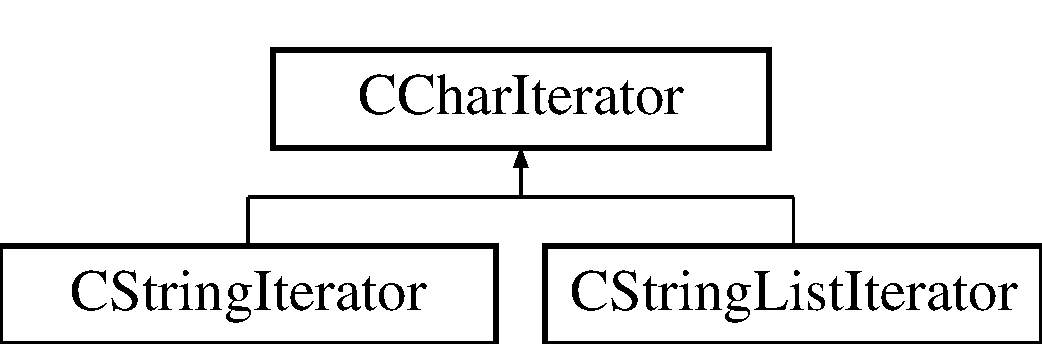
\includegraphics[height=2.000000cm]{df/d5a/classCCharIterator}
\end{center}
\end{figure}
\subsection*{Public Member Functions}
\begin{DoxyCompactItemize}
\item 
virtual int \hyperlink{classCCharIterator_af76726073a2c137b42031206da3fd077}{First\-Position} (void)
\item 
virtual int \hyperlink{classCCharIterator_a0bb27af4d399d1104a0ac630dad15551}{This\-Position} (void)
\item 
virtual int \hyperlink{classCCharIterator_a8c8c9299de7a6f743f038a8eff713331}{Last\-Position} (void)
\item 
virtual char \& \hyperlink{classCCharIterator_abc3cf59a2d2e08cf9dc472fc3586fe1d}{First} (void)
\item 
virtual char \& \hyperlink{classCCharIterator_a84808ea6da1bff06b9528068c3b67eb6}{Prev} (void)
\item 
virtual char \& \hyperlink{classCCharIterator_ab7ccc7e2891c3cd4ed9b08aef30f1a17}{This} (void)
\item 
virtual char \& \hyperlink{classCCharIterator_aa432eb048079b39a13d6147d8d977a0d}{Next} (void)
\item 
virtual char \& \hyperlink{classCCharIterator_a41a44b4c83aca6b35dd1ebd6d27e4fbb}{Last} (void)
\item 
virtual void \hyperlink{classCCharIterator_ac72db043fb84594bddf6fade20b906de}{Reset} (void)
\item 
virtual bool \hyperlink{classCCharIterator_a41cb29bdf53b99947a8f2a8c7894c7fe}{Match} (const \hyperlink{classCString}{C\-String} \&Pattern, const bool Move=false)
\item 
virtual void \hyperlink{classCCharIterator_a84ddcc0e6e24b12dd4883b11a1da48e2}{Print} (std\-::ostream \&out)
\item 
\hyperlink{classCCharIterator_a4e9b0b7376aafd366196a73d16d09c85}{C\-Char\-Iterator} (void)
\item 
\hyperlink{classCCharIterator_a4057437a5927e30014fc901cc6f11edd}{C\-Char\-Iterator} (const \hyperlink{classCCharIterator}{C\-Char\-Iterator} \&A\-Char\-Iterator)
\item 
virtual \hyperlink{classCCharIterator_a9cc988eac3b692b0451faba730ffa9b4}{$\sim$\-C\-Char\-Iterator} (void)
\end{DoxyCompactItemize}
\subsection*{Protected Attributes}
\begin{DoxyCompactItemize}
\item 
char \hyperlink{classCCharIterator_ae7690621a79350973df240ef49f579cc}{m\-\_\-\-Null\-Char}
\end{DoxyCompactItemize}


\subsection{Constructor \& Destructor Documentation}
\hypertarget{classCCharIterator_a4e9b0b7376aafd366196a73d16d09c85}{\index{C\-Char\-Iterator@{C\-Char\-Iterator}!C\-Char\-Iterator@{C\-Char\-Iterator}}
\index{C\-Char\-Iterator@{C\-Char\-Iterator}!CCharIterator@{C\-Char\-Iterator}}
\subsubsection[{C\-Char\-Iterator}]{\setlength{\rightskip}{0pt plus 5cm}C\-Char\-Iterator\-::\-C\-Char\-Iterator (
\begin{DoxyParamCaption}
\item[{void}]{}
\end{DoxyParamCaption}
)\hspace{0.3cm}{\ttfamily [inline]}}}\label{classCCharIterator_a4e9b0b7376aafd366196a73d16d09c85}
\hypertarget{classCCharIterator_a4057437a5927e30014fc901cc6f11edd}{\index{C\-Char\-Iterator@{C\-Char\-Iterator}!C\-Char\-Iterator@{C\-Char\-Iterator}}
\index{C\-Char\-Iterator@{C\-Char\-Iterator}!CCharIterator@{C\-Char\-Iterator}}
\subsubsection[{C\-Char\-Iterator}]{\setlength{\rightskip}{0pt plus 5cm}C\-Char\-Iterator\-::\-C\-Char\-Iterator (
\begin{DoxyParamCaption}
\item[{const {\bf C\-Char\-Iterator} \&}]{A\-Char\-Iterator}
\end{DoxyParamCaption}
)\hspace{0.3cm}{\ttfamily [inline]}}}\label{classCCharIterator_a4057437a5927e30014fc901cc6f11edd}
\hypertarget{classCCharIterator_a9cc988eac3b692b0451faba730ffa9b4}{\index{C\-Char\-Iterator@{C\-Char\-Iterator}!$\sim$\-C\-Char\-Iterator@{$\sim$\-C\-Char\-Iterator}}
\index{$\sim$\-C\-Char\-Iterator@{$\sim$\-C\-Char\-Iterator}!CCharIterator@{C\-Char\-Iterator}}
\subsubsection[{$\sim$\-C\-Char\-Iterator}]{\setlength{\rightskip}{0pt plus 5cm}virtual C\-Char\-Iterator\-::$\sim$\-C\-Char\-Iterator (
\begin{DoxyParamCaption}
\item[{void}]{}
\end{DoxyParamCaption}
)\hspace{0.3cm}{\ttfamily [inline]}, {\ttfamily [virtual]}}}\label{classCCharIterator_a9cc988eac3b692b0451faba730ffa9b4}


\subsection{Member Function Documentation}
\hypertarget{classCCharIterator_abc3cf59a2d2e08cf9dc472fc3586fe1d}{\index{C\-Char\-Iterator@{C\-Char\-Iterator}!First@{First}}
\index{First@{First}!CCharIterator@{C\-Char\-Iterator}}
\subsubsection[{First}]{\setlength{\rightskip}{0pt plus 5cm}virtual char\& C\-Char\-Iterator\-::\-First (
\begin{DoxyParamCaption}
\item[{void}]{}
\end{DoxyParamCaption}
)\hspace{0.3cm}{\ttfamily [inline]}, {\ttfamily [virtual]}}}\label{classCCharIterator_abc3cf59a2d2e08cf9dc472fc3586fe1d}


Reimplemented in \hyperlink{classCStringListIterator_aa127fde2929398c344504f500849fcb1}{C\-String\-List\-Iterator}, and \hyperlink{classCStringIterator_a606e84881c06c75e32399be5e89d8542}{C\-String\-Iterator}.

\hypertarget{classCCharIterator_af76726073a2c137b42031206da3fd077}{\index{C\-Char\-Iterator@{C\-Char\-Iterator}!First\-Position@{First\-Position}}
\index{First\-Position@{First\-Position}!CCharIterator@{C\-Char\-Iterator}}
\subsubsection[{First\-Position}]{\setlength{\rightskip}{0pt plus 5cm}virtual int C\-Char\-Iterator\-::\-First\-Position (
\begin{DoxyParamCaption}
\item[{void}]{}
\end{DoxyParamCaption}
)\hspace{0.3cm}{\ttfamily [inline]}, {\ttfamily [virtual]}}}\label{classCCharIterator_af76726073a2c137b42031206da3fd077}


Reimplemented in \hyperlink{classCStringListIterator_a0bde6983a18673bebfe0eed958231083}{C\-String\-List\-Iterator}, and \hyperlink{classCStringIterator_a739e5b2467a7fcda22960e857dd2ecc2}{C\-String\-Iterator}.

\hypertarget{classCCharIterator_a41a44b4c83aca6b35dd1ebd6d27e4fbb}{\index{C\-Char\-Iterator@{C\-Char\-Iterator}!Last@{Last}}
\index{Last@{Last}!CCharIterator@{C\-Char\-Iterator}}
\subsubsection[{Last}]{\setlength{\rightskip}{0pt plus 5cm}virtual char\& C\-Char\-Iterator\-::\-Last (
\begin{DoxyParamCaption}
\item[{void}]{}
\end{DoxyParamCaption}
)\hspace{0.3cm}{\ttfamily [inline]}, {\ttfamily [virtual]}}}\label{classCCharIterator_a41a44b4c83aca6b35dd1ebd6d27e4fbb}


Reimplemented in \hyperlink{classCStringListIterator_a2801731076eae0d85a8037aa746b0e3b}{C\-String\-List\-Iterator}, and \hyperlink{classCStringIterator_aa8a8dab6db490395dba9d522d6cead2f}{C\-String\-Iterator}.

\hypertarget{classCCharIterator_a8c8c9299de7a6f743f038a8eff713331}{\index{C\-Char\-Iterator@{C\-Char\-Iterator}!Last\-Position@{Last\-Position}}
\index{Last\-Position@{Last\-Position}!CCharIterator@{C\-Char\-Iterator}}
\subsubsection[{Last\-Position}]{\setlength{\rightskip}{0pt plus 5cm}virtual int C\-Char\-Iterator\-::\-Last\-Position (
\begin{DoxyParamCaption}
\item[{void}]{}
\end{DoxyParamCaption}
)\hspace{0.3cm}{\ttfamily [inline]}, {\ttfamily [virtual]}}}\label{classCCharIterator_a8c8c9299de7a6f743f038a8eff713331}


Reimplemented in \hyperlink{classCStringListIterator_afc5a0d463ea6783767dad416211318fc}{C\-String\-List\-Iterator}, and \hyperlink{classCStringIterator_ad999b0402cd3261b42e2a6395fd483cb}{C\-String\-Iterator}.

\hypertarget{classCCharIterator_a41cb29bdf53b99947a8f2a8c7894c7fe}{\index{C\-Char\-Iterator@{C\-Char\-Iterator}!Match@{Match}}
\index{Match@{Match}!CCharIterator@{C\-Char\-Iterator}}
\subsubsection[{Match}]{\setlength{\rightskip}{0pt plus 5cm}bool C\-Char\-Iterator\-::\-Match (
\begin{DoxyParamCaption}
\item[{const {\bf C\-String} \&}]{Pattern, }
\item[{const bool}]{Move = {\ttfamily false}}
\end{DoxyParamCaption}
)\hspace{0.3cm}{\ttfamily [virtual]}}}\label{classCCharIterator_a41cb29bdf53b99947a8f2a8c7894c7fe}


Reimplemented in \hyperlink{classCStringListIterator_a42f9aed958e2d8217ac672e80b488f0a}{C\-String\-List\-Iterator}, and \hyperlink{classCStringIterator_a942c6a942235d37549673ca0d9772614}{C\-String\-Iterator}.

\hypertarget{classCCharIterator_aa432eb048079b39a13d6147d8d977a0d}{\index{C\-Char\-Iterator@{C\-Char\-Iterator}!Next@{Next}}
\index{Next@{Next}!CCharIterator@{C\-Char\-Iterator}}
\subsubsection[{Next}]{\setlength{\rightskip}{0pt plus 5cm}virtual char\& C\-Char\-Iterator\-::\-Next (
\begin{DoxyParamCaption}
\item[{void}]{}
\end{DoxyParamCaption}
)\hspace{0.3cm}{\ttfamily [inline]}, {\ttfamily [virtual]}}}\label{classCCharIterator_aa432eb048079b39a13d6147d8d977a0d}


Reimplemented in \hyperlink{classCStringListIterator_aa4625f7dc1225aaae83f9154d44aec38}{C\-String\-List\-Iterator}, and \hyperlink{classCStringIterator_a04eb992396cb473486cd13982974d984}{C\-String\-Iterator}.

\hypertarget{classCCharIterator_a84808ea6da1bff06b9528068c3b67eb6}{\index{C\-Char\-Iterator@{C\-Char\-Iterator}!Prev@{Prev}}
\index{Prev@{Prev}!CCharIterator@{C\-Char\-Iterator}}
\subsubsection[{Prev}]{\setlength{\rightskip}{0pt plus 5cm}virtual char\& C\-Char\-Iterator\-::\-Prev (
\begin{DoxyParamCaption}
\item[{void}]{}
\end{DoxyParamCaption}
)\hspace{0.3cm}{\ttfamily [inline]}, {\ttfamily [virtual]}}}\label{classCCharIterator_a84808ea6da1bff06b9528068c3b67eb6}


Reimplemented in \hyperlink{classCStringListIterator_a8b82110c52fedd6cb18660526c63f8ef}{C\-String\-List\-Iterator}, and \hyperlink{classCStringIterator_adc6c3c8fd47262015aff531a8fea44b3}{C\-String\-Iterator}.

\hypertarget{classCCharIterator_a84ddcc0e6e24b12dd4883b11a1da48e2}{\index{C\-Char\-Iterator@{C\-Char\-Iterator}!Print@{Print}}
\index{Print@{Print}!CCharIterator@{C\-Char\-Iterator}}
\subsubsection[{Print}]{\setlength{\rightskip}{0pt plus 5cm}virtual void C\-Char\-Iterator\-::\-Print (
\begin{DoxyParamCaption}
\item[{std\-::ostream \&}]{out}
\end{DoxyParamCaption}
)\hspace{0.3cm}{\ttfamily [inline]}, {\ttfamily [virtual]}}}\label{classCCharIterator_a84ddcc0e6e24b12dd4883b11a1da48e2}
\hypertarget{classCCharIterator_ac72db043fb84594bddf6fade20b906de}{\index{C\-Char\-Iterator@{C\-Char\-Iterator}!Reset@{Reset}}
\index{Reset@{Reset}!CCharIterator@{C\-Char\-Iterator}}
\subsubsection[{Reset}]{\setlength{\rightskip}{0pt plus 5cm}virtual void C\-Char\-Iterator\-::\-Reset (
\begin{DoxyParamCaption}
\item[{void}]{}
\end{DoxyParamCaption}
)\hspace{0.3cm}{\ttfamily [inline]}, {\ttfamily [virtual]}}}\label{classCCharIterator_ac72db043fb84594bddf6fade20b906de}


Reimplemented in \hyperlink{classCStringListIterator_af3d67cf68505a00289ffd271215d1254}{C\-String\-List\-Iterator}, and \hyperlink{classCStringIterator_a4b926ac119cd8a0a6279e149a1ed4c73}{C\-String\-Iterator}.

\hypertarget{classCCharIterator_ab7ccc7e2891c3cd4ed9b08aef30f1a17}{\index{C\-Char\-Iterator@{C\-Char\-Iterator}!This@{This}}
\index{This@{This}!CCharIterator@{C\-Char\-Iterator}}
\subsubsection[{This}]{\setlength{\rightskip}{0pt plus 5cm}virtual char\& C\-Char\-Iterator\-::\-This (
\begin{DoxyParamCaption}
\item[{void}]{}
\end{DoxyParamCaption}
)\hspace{0.3cm}{\ttfamily [inline]}, {\ttfamily [virtual]}}}\label{classCCharIterator_ab7ccc7e2891c3cd4ed9b08aef30f1a17}


Reimplemented in \hyperlink{classCStringListIterator_ab163a0cda37b05ce985f876245bc8cd2}{C\-String\-List\-Iterator}, and \hyperlink{classCStringIterator_aac7b3adb4f5d80c98399c4fe587f4c4b}{C\-String\-Iterator}.

\hypertarget{classCCharIterator_a0bb27af4d399d1104a0ac630dad15551}{\index{C\-Char\-Iterator@{C\-Char\-Iterator}!This\-Position@{This\-Position}}
\index{This\-Position@{This\-Position}!CCharIterator@{C\-Char\-Iterator}}
\subsubsection[{This\-Position}]{\setlength{\rightskip}{0pt plus 5cm}virtual int C\-Char\-Iterator\-::\-This\-Position (
\begin{DoxyParamCaption}
\item[{void}]{}
\end{DoxyParamCaption}
)\hspace{0.3cm}{\ttfamily [inline]}, {\ttfamily [virtual]}}}\label{classCCharIterator_a0bb27af4d399d1104a0ac630dad15551}


Reimplemented in \hyperlink{classCStringListIterator_a369446781e7b62abc79311f73bd9c54a}{C\-String\-List\-Iterator}, and \hyperlink{classCStringIterator_af71c8376f7118488e50d274ff0929941}{C\-String\-Iterator}.



\subsection{Member Data Documentation}
\hypertarget{classCCharIterator_ae7690621a79350973df240ef49f579cc}{\index{C\-Char\-Iterator@{C\-Char\-Iterator}!m\-\_\-\-Null\-Char@{m\-\_\-\-Null\-Char}}
\index{m\-\_\-\-Null\-Char@{m\-\_\-\-Null\-Char}!CCharIterator@{C\-Char\-Iterator}}
\subsubsection[{m\-\_\-\-Null\-Char}]{\setlength{\rightskip}{0pt plus 5cm}char C\-Char\-Iterator\-::m\-\_\-\-Null\-Char\hspace{0.3cm}{\ttfamily [protected]}}}\label{classCCharIterator_ae7690621a79350973df240ef49f579cc}


The documentation for this class was generated from the following files\-:\begin{DoxyCompactItemize}
\item 
lib/\hyperlink{stlstrings_8h}{stlstrings.\-h}\item 
lib/\hyperlink{stlstrings_8cpp}{stlstrings.\-cpp}\end{DoxyCompactItemize}

\hypertarget{classCCharset}{\section{C\-Charset Class Reference}
\label{classCCharset}\index{C\-Charset@{C\-Charset}}
}


{\ttfamily \#include $<$stlstrings.\-h$>$}

\subsection*{Public Member Functions}
\begin{DoxyCompactItemize}
\item 
bool \hyperlink{classCCharset_afc2bdd38fc4a5a76f79c384b7e010949}{Isset} (const char A\-Char) const 
\item 
char \hyperlink{classCCharset_a57c884b268bdf924a8eea466d83bb0c3}{Get\-Char} (const char A\-Char) const 
\item 
void \hyperlink{classCCharset_a83fb686e1529fd7756e2518fa3aada35}{Set\-Char} (const char A\-Char)
\item 
void \hyperlink{classCCharset_a3ba43c6f02804f2d8e5e975f884d7f67}{Unset\-Char} (const char A\-Char)
\item 
\hyperlink{classCString}{C\-String} \hyperlink{classCCharset_af103cfcfd67bb0a0c605cae9104324c4}{Get\-Alphabet} (void) const 
\item 
void \hyperlink{classCCharset_a03a13466cc53fee97df68fdffe66e265}{Set\-Alphabet} (const \hyperlink{classCString}{C\-String} \&Alphabet)
\item 
void \hyperlink{classCCharset_a2890d5eda53b22f39b33b5c1eca3b369}{Print} (std\-::ostream \&out)
\item 
\hyperlink{classCCharset_a550b4d6acc0ff40babaa01eb5391954f}{C\-Charset} (void)
\item 
\hyperlink{classCCharset_aee827626805ed9382333323f75062296}{C\-Charset} (const \hyperlink{classCCharset}{C\-Charset} \&Charset)
\item 
\hyperlink{classCCharset_a63eb516c33dc84299d1269ffada3045c}{C\-Charset} (const \hyperlink{classCString}{C\-String} \&Alphabet)
\item 
\hyperlink{classCCharset_a6dd837f6b29926022feab11d04921cd2}{$\sim$\-C\-Charset} (void)
\end{DoxyCompactItemize}
\subsection*{Protected Member Functions}
\begin{DoxyCompactItemize}
\item 
void \hyperlink{classCCharset_ada7eed949293b0202f3cb35aeee6b6f9}{Update\-Charset} (void)
\item 
void \hyperlink{classCCharset_acd9542af26449bec96d5bd7dc36285fe}{Update\-Alphabet} (void)
\end{DoxyCompactItemize}
\subsection*{Protected Attributes}
\begin{DoxyCompactItemize}
\item 
bool \hyperlink{classCCharset_abe4fd67584bdae559b63afc6dd873686}{m\-\_\-\-Charset} \mbox{[}\hyperlink{stlstrings_8h_a8085b77b952d20d37d96fff6a294be34}{C\-H\-A\-R\-S\-E\-T\-\_\-\-S\-I\-Z\-E}\mbox{]}
\item 
\hyperlink{classCString}{C\-String} \hyperlink{classCCharset_ac6e379b2a505801ede9713ba04de0a8b}{m\-\_\-\-Alphabet}
\end{DoxyCompactItemize}


\subsection{Constructor \& Destructor Documentation}
\hypertarget{classCCharset_a550b4d6acc0ff40babaa01eb5391954f}{\index{C\-Charset@{C\-Charset}!C\-Charset@{C\-Charset}}
\index{C\-Charset@{C\-Charset}!CCharset@{C\-Charset}}
\subsubsection[{C\-Charset}]{\setlength{\rightskip}{0pt plus 5cm}C\-Charset\-::\-C\-Charset (
\begin{DoxyParamCaption}
\item[{void}]{}
\end{DoxyParamCaption}
)}}\label{classCCharset_a550b4d6acc0ff40babaa01eb5391954f}
\hypertarget{classCCharset_aee827626805ed9382333323f75062296}{\index{C\-Charset@{C\-Charset}!C\-Charset@{C\-Charset}}
\index{C\-Charset@{C\-Charset}!CCharset@{C\-Charset}}
\subsubsection[{C\-Charset}]{\setlength{\rightskip}{0pt plus 5cm}C\-Charset\-::\-C\-Charset (
\begin{DoxyParamCaption}
\item[{const {\bf C\-Charset} \&}]{Charset}
\end{DoxyParamCaption}
)}}\label{classCCharset_aee827626805ed9382333323f75062296}
\hypertarget{classCCharset_a63eb516c33dc84299d1269ffada3045c}{\index{C\-Charset@{C\-Charset}!C\-Charset@{C\-Charset}}
\index{C\-Charset@{C\-Charset}!CCharset@{C\-Charset}}
\subsubsection[{C\-Charset}]{\setlength{\rightskip}{0pt plus 5cm}C\-Charset\-::\-C\-Charset (
\begin{DoxyParamCaption}
\item[{const {\bf C\-String} \&}]{Alphabet}
\end{DoxyParamCaption}
)}}\label{classCCharset_a63eb516c33dc84299d1269ffada3045c}
\hypertarget{classCCharset_a6dd837f6b29926022feab11d04921cd2}{\index{C\-Charset@{C\-Charset}!$\sim$\-C\-Charset@{$\sim$\-C\-Charset}}
\index{$\sim$\-C\-Charset@{$\sim$\-C\-Charset}!CCharset@{C\-Charset}}
\subsubsection[{$\sim$\-C\-Charset}]{\setlength{\rightskip}{0pt plus 5cm}C\-Charset\-::$\sim$\-C\-Charset (
\begin{DoxyParamCaption}
\item[{void}]{}
\end{DoxyParamCaption}
)}}\label{classCCharset_a6dd837f6b29926022feab11d04921cd2}


\subsection{Member Function Documentation}
\hypertarget{classCCharset_af103cfcfd67bb0a0c605cae9104324c4}{\index{C\-Charset@{C\-Charset}!Get\-Alphabet@{Get\-Alphabet}}
\index{Get\-Alphabet@{Get\-Alphabet}!CCharset@{C\-Charset}}
\subsubsection[{Get\-Alphabet}]{\setlength{\rightskip}{0pt plus 5cm}{\bf C\-String} C\-Charset\-::\-Get\-Alphabet (
\begin{DoxyParamCaption}
\item[{void}]{}
\end{DoxyParamCaption}
) const}}\label{classCCharset_af103cfcfd67bb0a0c605cae9104324c4}
\hypertarget{classCCharset_a57c884b268bdf924a8eea466d83bb0c3}{\index{C\-Charset@{C\-Charset}!Get\-Char@{Get\-Char}}
\index{Get\-Char@{Get\-Char}!CCharset@{C\-Charset}}
\subsubsection[{Get\-Char}]{\setlength{\rightskip}{0pt plus 5cm}char C\-Charset\-::\-Get\-Char (
\begin{DoxyParamCaption}
\item[{const char}]{A\-Char}
\end{DoxyParamCaption}
) const}}\label{classCCharset_a57c884b268bdf924a8eea466d83bb0c3}
\hypertarget{classCCharset_afc2bdd38fc4a5a76f79c384b7e010949}{\index{C\-Charset@{C\-Charset}!Isset@{Isset}}
\index{Isset@{Isset}!CCharset@{C\-Charset}}
\subsubsection[{Isset}]{\setlength{\rightskip}{0pt plus 5cm}bool C\-Charset\-::\-Isset (
\begin{DoxyParamCaption}
\item[{const char}]{A\-Char}
\end{DoxyParamCaption}
) const}}\label{classCCharset_afc2bdd38fc4a5a76f79c384b7e010949}
\hypertarget{classCCharset_a2890d5eda53b22f39b33b5c1eca3b369}{\index{C\-Charset@{C\-Charset}!Print@{Print}}
\index{Print@{Print}!CCharset@{C\-Charset}}
\subsubsection[{Print}]{\setlength{\rightskip}{0pt plus 5cm}void C\-Charset\-::\-Print (
\begin{DoxyParamCaption}
\item[{std\-::ostream \&}]{out}
\end{DoxyParamCaption}
)}}\label{classCCharset_a2890d5eda53b22f39b33b5c1eca3b369}
\hypertarget{classCCharset_a03a13466cc53fee97df68fdffe66e265}{\index{C\-Charset@{C\-Charset}!Set\-Alphabet@{Set\-Alphabet}}
\index{Set\-Alphabet@{Set\-Alphabet}!CCharset@{C\-Charset}}
\subsubsection[{Set\-Alphabet}]{\setlength{\rightskip}{0pt plus 5cm}void C\-Charset\-::\-Set\-Alphabet (
\begin{DoxyParamCaption}
\item[{const {\bf C\-String} \&}]{Alphabet}
\end{DoxyParamCaption}
)}}\label{classCCharset_a03a13466cc53fee97df68fdffe66e265}
\hypertarget{classCCharset_a83fb686e1529fd7756e2518fa3aada35}{\index{C\-Charset@{C\-Charset}!Set\-Char@{Set\-Char}}
\index{Set\-Char@{Set\-Char}!CCharset@{C\-Charset}}
\subsubsection[{Set\-Char}]{\setlength{\rightskip}{0pt plus 5cm}void C\-Charset\-::\-Set\-Char (
\begin{DoxyParamCaption}
\item[{const char}]{A\-Char}
\end{DoxyParamCaption}
)}}\label{classCCharset_a83fb686e1529fd7756e2518fa3aada35}
\hypertarget{classCCharset_a3ba43c6f02804f2d8e5e975f884d7f67}{\index{C\-Charset@{C\-Charset}!Unset\-Char@{Unset\-Char}}
\index{Unset\-Char@{Unset\-Char}!CCharset@{C\-Charset}}
\subsubsection[{Unset\-Char}]{\setlength{\rightskip}{0pt plus 5cm}void C\-Charset\-::\-Unset\-Char (
\begin{DoxyParamCaption}
\item[{const char}]{A\-Char}
\end{DoxyParamCaption}
)}}\label{classCCharset_a3ba43c6f02804f2d8e5e975f884d7f67}
\hypertarget{classCCharset_acd9542af26449bec96d5bd7dc36285fe}{\index{C\-Charset@{C\-Charset}!Update\-Alphabet@{Update\-Alphabet}}
\index{Update\-Alphabet@{Update\-Alphabet}!CCharset@{C\-Charset}}
\subsubsection[{Update\-Alphabet}]{\setlength{\rightskip}{0pt plus 5cm}void C\-Charset\-::\-Update\-Alphabet (
\begin{DoxyParamCaption}
\item[{void}]{}
\end{DoxyParamCaption}
)\hspace{0.3cm}{\ttfamily [protected]}}}\label{classCCharset_acd9542af26449bec96d5bd7dc36285fe}
\hypertarget{classCCharset_ada7eed949293b0202f3cb35aeee6b6f9}{\index{C\-Charset@{C\-Charset}!Update\-Charset@{Update\-Charset}}
\index{Update\-Charset@{Update\-Charset}!CCharset@{C\-Charset}}
\subsubsection[{Update\-Charset}]{\setlength{\rightskip}{0pt plus 5cm}void C\-Charset\-::\-Update\-Charset (
\begin{DoxyParamCaption}
\item[{void}]{}
\end{DoxyParamCaption}
)\hspace{0.3cm}{\ttfamily [protected]}}}\label{classCCharset_ada7eed949293b0202f3cb35aeee6b6f9}


\subsection{Member Data Documentation}
\hypertarget{classCCharset_ac6e379b2a505801ede9713ba04de0a8b}{\index{C\-Charset@{C\-Charset}!m\-\_\-\-Alphabet@{m\-\_\-\-Alphabet}}
\index{m\-\_\-\-Alphabet@{m\-\_\-\-Alphabet}!CCharset@{C\-Charset}}
\subsubsection[{m\-\_\-\-Alphabet}]{\setlength{\rightskip}{0pt plus 5cm}{\bf C\-String} C\-Charset\-::m\-\_\-\-Alphabet\hspace{0.3cm}{\ttfamily [protected]}}}\label{classCCharset_ac6e379b2a505801ede9713ba04de0a8b}
\hypertarget{classCCharset_abe4fd67584bdae559b63afc6dd873686}{\index{C\-Charset@{C\-Charset}!m\-\_\-\-Charset@{m\-\_\-\-Charset}}
\index{m\-\_\-\-Charset@{m\-\_\-\-Charset}!CCharset@{C\-Charset}}
\subsubsection[{m\-\_\-\-Charset}]{\setlength{\rightskip}{0pt plus 5cm}bool C\-Charset\-::m\-\_\-\-Charset\mbox{[}{\bf C\-H\-A\-R\-S\-E\-T\-\_\-\-S\-I\-Z\-E}\mbox{]}\hspace{0.3cm}{\ttfamily [protected]}}}\label{classCCharset_abe4fd67584bdae559b63afc6dd873686}


The documentation for this class was generated from the following files\-:\begin{DoxyCompactItemize}
\item 
lib/\hyperlink{stlstrings_8h}{stlstrings.\-h}\item 
lib/\hyperlink{stlstrings_8cpp}{stlstrings.\-cpp}\end{DoxyCompactItemize}

\hypertarget{classCCharVariable}{\section{C\-Char\-Variable Class Reference}
\label{classCCharVariable}\index{C\-Char\-Variable@{C\-Char\-Variable}}
}


{\ttfamily \#include $<$stlvariables.\-h$>$}

Inheritance diagram for C\-Char\-Variable\-:\begin{figure}[H]
\begin{center}
\leavevmode
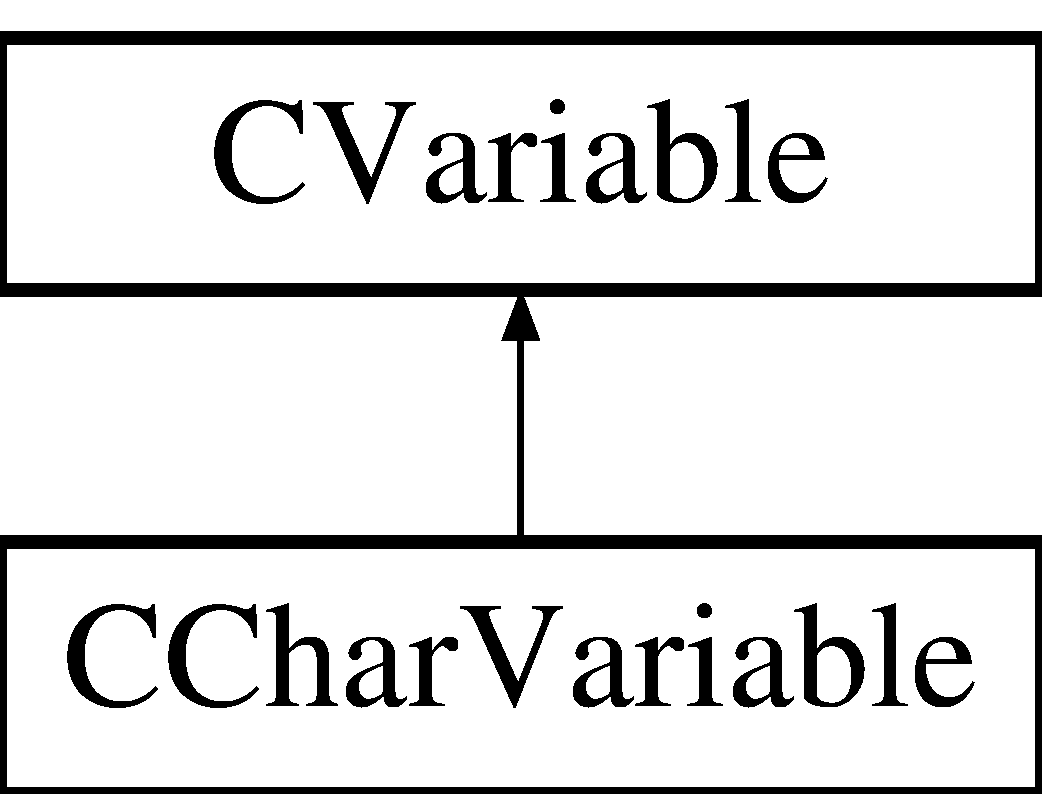
\includegraphics[height=2.000000cm]{d3/daa/classCCharVariable}
\end{center}
\end{figure}
\subsection*{Public Member Functions}
\begin{DoxyCompactItemize}
\item 
virtual int \hyperlink{classCCharVariable_affc9e6d08fd02a634051d1f93a17daae}{Get\-Type} (void) const 
\item 
virtual \hyperlink{classCString}{C\-String} \hyperlink{classCCharVariable_a074d079d84d374fd3e5ad5450481dbd4}{Get\-Type\-Name} (void) const 
\item 
virtual double \hyperlink{classCCharVariable_ac99bc24b9317a3dfbcca74323a501b34}{Get\-Float} (void) const 
\item 
virtual void \hyperlink{classCCharVariable_aba3a833cbd4d2e135c30f6057cb7b925}{Set\-Float} (const double Value)
\item 
virtual int \hyperlink{classCCharVariable_a2fa1f3606008449057020fe408cfb14b}{Get\-Integer} (void) const 
\item 
virtual void \hyperlink{classCCharVariable_a2c09cdde57df25e1ea9b05a024e88351}{Set\-Integer} (const int Value)
\item 
virtual bool \hyperlink{classCCharVariable_ac84ca3b9594858ac0fed4dde57388e85}{Get\-Boolean} (void) const 
\item 
virtual void \hyperlink{classCCharVariable_a3a5d6e88ed9281e6d8c6833826266398}{Set\-Boolean} (const bool Value)
\item 
virtual \hyperlink{classCString}{C\-String} \hyperlink{classCCharVariable_aedfd33f26e2e746e2631e9267e602e3a}{Get\-String} (void) const 
\item 
virtual void \hyperlink{classCCharVariable_a534d79a4b878a3c6fe13d6681b27eed3}{Set\-String} (const \hyperlink{classCString}{C\-String} \&Value)
\item 
virtual char \hyperlink{classCCharVariable_a8f9dab783a2dd3ca945b614d5338cfa5}{Get\-Char} (void) const 
\item 
virtual void \hyperlink{classCCharVariable_acd18202ed2d51ae71c61825a70aed8f6}{Set\-Char} (const char Value)
\item 
char \hyperlink{classCCharVariable_a925186465e82d1e4176e71d0570eb78f}{operator=} (const \hyperlink{classCCharVariable}{C\-Char\-Variable} \&Variable)
\item 
\hyperlink{classCCharVariable}{C\-Char\-Variable} \& \hyperlink{classCCharVariable_a62299b37fe7af7a738ad7560def8af11}{operator=} (const double Value)
\item 
\hyperlink{classCCharVariable}{C\-Char\-Variable} \& \hyperlink{classCCharVariable_a6b23a1db0dc1c7e0f9b5d300afce1f39}{operator=} (const int Value)
\item 
\hyperlink{classCCharVariable}{C\-Char\-Variable} \& \hyperlink{classCCharVariable_ad462dd5286582fc983efd78fa0f9eb6b}{operator=} (const bool Value)
\item 
\hyperlink{classCCharVariable}{C\-Char\-Variable} \& \hyperlink{classCCharVariable_a2a898698c674e16474eaef2ebba5b3fc}{operator=} (const \hyperlink{classCString}{C\-String} \&Value)
\item 
\hyperlink{classCCharVariable}{C\-Char\-Variable} \& \hyperlink{classCCharVariable_a5067c8967f080401e47156c1745e954d}{operator=} (const char Value)
\item 
\hyperlink{classCCharVariable_a60d5255de8d6661ee6a195284f144c50}{C\-Char\-Variable} (const \hyperlink{classCString}{C\-String} \&Name, const char Value=char(0))
\item 
virtual \hyperlink{classCCharVariable_a8c8be62cf2960f61f0275c2b35d479a2}{$\sim$\-C\-Char\-Variable} (void)
\end{DoxyCompactItemize}
\subsection*{Protected Attributes}
\begin{DoxyCompactItemize}
\item 
char \hyperlink{classCCharVariable_a0e76b26ffd276425d7bf5fe80dd118f2}{m\-\_\-\-Value}
\end{DoxyCompactItemize}


\subsection{Constructor \& Destructor Documentation}
\hypertarget{classCCharVariable_a60d5255de8d6661ee6a195284f144c50}{\index{C\-Char\-Variable@{C\-Char\-Variable}!C\-Char\-Variable@{C\-Char\-Variable}}
\index{C\-Char\-Variable@{C\-Char\-Variable}!CCharVariable@{C\-Char\-Variable}}
\subsubsection[{C\-Char\-Variable}]{\setlength{\rightskip}{0pt plus 5cm}C\-Char\-Variable\-::\-C\-Char\-Variable (
\begin{DoxyParamCaption}
\item[{const {\bf C\-String} \&}]{Name, }
\item[{const char}]{Value = {\ttfamily char(0)}}
\end{DoxyParamCaption}
)}}\label{classCCharVariable_a60d5255de8d6661ee6a195284f144c50}
\hypertarget{classCCharVariable_a8c8be62cf2960f61f0275c2b35d479a2}{\index{C\-Char\-Variable@{C\-Char\-Variable}!$\sim$\-C\-Char\-Variable@{$\sim$\-C\-Char\-Variable}}
\index{$\sim$\-C\-Char\-Variable@{$\sim$\-C\-Char\-Variable}!CCharVariable@{C\-Char\-Variable}}
\subsubsection[{$\sim$\-C\-Char\-Variable}]{\setlength{\rightskip}{0pt plus 5cm}virtual C\-Char\-Variable\-::$\sim$\-C\-Char\-Variable (
\begin{DoxyParamCaption}
\item[{void}]{}
\end{DoxyParamCaption}
)\hspace{0.3cm}{\ttfamily [inline]}, {\ttfamily [virtual]}}}\label{classCCharVariable_a8c8be62cf2960f61f0275c2b35d479a2}


\subsection{Member Function Documentation}
\hypertarget{classCCharVariable_ac84ca3b9594858ac0fed4dde57388e85}{\index{C\-Char\-Variable@{C\-Char\-Variable}!Get\-Boolean@{Get\-Boolean}}
\index{Get\-Boolean@{Get\-Boolean}!CCharVariable@{C\-Char\-Variable}}
\subsubsection[{Get\-Boolean}]{\setlength{\rightskip}{0pt plus 5cm}bool C\-Char\-Variable\-::\-Get\-Boolean (
\begin{DoxyParamCaption}
\item[{void}]{}
\end{DoxyParamCaption}
) const\hspace{0.3cm}{\ttfamily [virtual]}}}\label{classCCharVariable_ac84ca3b9594858ac0fed4dde57388e85}


Reimplemented from \hyperlink{classCVariable_a874156d6b1a3a44f799c32a2455c7f49}{C\-Variable}.

\hypertarget{classCCharVariable_a8f9dab783a2dd3ca945b614d5338cfa5}{\index{C\-Char\-Variable@{C\-Char\-Variable}!Get\-Char@{Get\-Char}}
\index{Get\-Char@{Get\-Char}!CCharVariable@{C\-Char\-Variable}}
\subsubsection[{Get\-Char}]{\setlength{\rightskip}{0pt plus 5cm}char C\-Char\-Variable\-::\-Get\-Char (
\begin{DoxyParamCaption}
\item[{void}]{}
\end{DoxyParamCaption}
) const\hspace{0.3cm}{\ttfamily [virtual]}}}\label{classCCharVariable_a8f9dab783a2dd3ca945b614d5338cfa5}


Reimplemented from \hyperlink{classCVariable_a6635a8fd2441dcb83a39d10a78187dac}{C\-Variable}.

\hypertarget{classCCharVariable_ac99bc24b9317a3dfbcca74323a501b34}{\index{C\-Char\-Variable@{C\-Char\-Variable}!Get\-Float@{Get\-Float}}
\index{Get\-Float@{Get\-Float}!CCharVariable@{C\-Char\-Variable}}
\subsubsection[{Get\-Float}]{\setlength{\rightskip}{0pt plus 5cm}double C\-Char\-Variable\-::\-Get\-Float (
\begin{DoxyParamCaption}
\item[{void}]{}
\end{DoxyParamCaption}
) const\hspace{0.3cm}{\ttfamily [virtual]}}}\label{classCCharVariable_ac99bc24b9317a3dfbcca74323a501b34}


Reimplemented from \hyperlink{classCVariable_ac475ad87ffbfaeeb2d4d9c2986b0d575}{C\-Variable}.

\hypertarget{classCCharVariable_a2fa1f3606008449057020fe408cfb14b}{\index{C\-Char\-Variable@{C\-Char\-Variable}!Get\-Integer@{Get\-Integer}}
\index{Get\-Integer@{Get\-Integer}!CCharVariable@{C\-Char\-Variable}}
\subsubsection[{Get\-Integer}]{\setlength{\rightskip}{0pt plus 5cm}int C\-Char\-Variable\-::\-Get\-Integer (
\begin{DoxyParamCaption}
\item[{void}]{}
\end{DoxyParamCaption}
) const\hspace{0.3cm}{\ttfamily [virtual]}}}\label{classCCharVariable_a2fa1f3606008449057020fe408cfb14b}


Reimplemented from \hyperlink{classCVariable_adb0db49f4a55f3e1b5322f6ce26e4ebc}{C\-Variable}.

\hypertarget{classCCharVariable_aedfd33f26e2e746e2631e9267e602e3a}{\index{C\-Char\-Variable@{C\-Char\-Variable}!Get\-String@{Get\-String}}
\index{Get\-String@{Get\-String}!CCharVariable@{C\-Char\-Variable}}
\subsubsection[{Get\-String}]{\setlength{\rightskip}{0pt plus 5cm}{\bf C\-String} C\-Char\-Variable\-::\-Get\-String (
\begin{DoxyParamCaption}
\item[{void}]{}
\end{DoxyParamCaption}
) const\hspace{0.3cm}{\ttfamily [virtual]}}}\label{classCCharVariable_aedfd33f26e2e746e2631e9267e602e3a}


Reimplemented from \hyperlink{classCVariable_aefa25c880c0042ffc29889475d329004}{C\-Variable}.

\hypertarget{classCCharVariable_affc9e6d08fd02a634051d1f93a17daae}{\index{C\-Char\-Variable@{C\-Char\-Variable}!Get\-Type@{Get\-Type}}
\index{Get\-Type@{Get\-Type}!CCharVariable@{C\-Char\-Variable}}
\subsubsection[{Get\-Type}]{\setlength{\rightskip}{0pt plus 5cm}int C\-Char\-Variable\-::\-Get\-Type (
\begin{DoxyParamCaption}
\item[{void}]{}
\end{DoxyParamCaption}
) const\hspace{0.3cm}{\ttfamily [virtual]}}}\label{classCCharVariable_affc9e6d08fd02a634051d1f93a17daae}


Reimplemented from \hyperlink{classCVariable_acdf7301ad2f5c7fa33770c028211c0bc}{C\-Variable}.

\hypertarget{classCCharVariable_a074d079d84d374fd3e5ad5450481dbd4}{\index{C\-Char\-Variable@{C\-Char\-Variable}!Get\-Type\-Name@{Get\-Type\-Name}}
\index{Get\-Type\-Name@{Get\-Type\-Name}!CCharVariable@{C\-Char\-Variable}}
\subsubsection[{Get\-Type\-Name}]{\setlength{\rightskip}{0pt plus 5cm}{\bf C\-String} C\-Char\-Variable\-::\-Get\-Type\-Name (
\begin{DoxyParamCaption}
\item[{void}]{}
\end{DoxyParamCaption}
) const\hspace{0.3cm}{\ttfamily [virtual]}}}\label{classCCharVariable_a074d079d84d374fd3e5ad5450481dbd4}


Reimplemented from \hyperlink{classCVariable_ad8a23d1501917cbfb1eee1473a7a2122}{C\-Variable}.

\hypertarget{classCCharVariable_a925186465e82d1e4176e71d0570eb78f}{\index{C\-Char\-Variable@{C\-Char\-Variable}!operator=@{operator=}}
\index{operator=@{operator=}!CCharVariable@{C\-Char\-Variable}}
\subsubsection[{operator=}]{\setlength{\rightskip}{0pt plus 5cm}char C\-Char\-Variable\-::operator= (
\begin{DoxyParamCaption}
\item[{const {\bf C\-Char\-Variable} \&}]{Variable}
\end{DoxyParamCaption}
)}}\label{classCCharVariable_a925186465e82d1e4176e71d0570eb78f}
\hypertarget{classCCharVariable_a62299b37fe7af7a738ad7560def8af11}{\index{C\-Char\-Variable@{C\-Char\-Variable}!operator=@{operator=}}
\index{operator=@{operator=}!CCharVariable@{C\-Char\-Variable}}
\subsubsection[{operator=}]{\setlength{\rightskip}{0pt plus 5cm}{\bf C\-Char\-Variable} \& C\-Char\-Variable\-::operator= (
\begin{DoxyParamCaption}
\item[{const double}]{Value}
\end{DoxyParamCaption}
)}}\label{classCCharVariable_a62299b37fe7af7a738ad7560def8af11}
\hypertarget{classCCharVariable_a6b23a1db0dc1c7e0f9b5d300afce1f39}{\index{C\-Char\-Variable@{C\-Char\-Variable}!operator=@{operator=}}
\index{operator=@{operator=}!CCharVariable@{C\-Char\-Variable}}
\subsubsection[{operator=}]{\setlength{\rightskip}{0pt plus 5cm}{\bf C\-Char\-Variable} \& C\-Char\-Variable\-::operator= (
\begin{DoxyParamCaption}
\item[{const int}]{Value}
\end{DoxyParamCaption}
)}}\label{classCCharVariable_a6b23a1db0dc1c7e0f9b5d300afce1f39}
\hypertarget{classCCharVariable_ad462dd5286582fc983efd78fa0f9eb6b}{\index{C\-Char\-Variable@{C\-Char\-Variable}!operator=@{operator=}}
\index{operator=@{operator=}!CCharVariable@{C\-Char\-Variable}}
\subsubsection[{operator=}]{\setlength{\rightskip}{0pt plus 5cm}{\bf C\-Char\-Variable} \& C\-Char\-Variable\-::operator= (
\begin{DoxyParamCaption}
\item[{const bool}]{Value}
\end{DoxyParamCaption}
)}}\label{classCCharVariable_ad462dd5286582fc983efd78fa0f9eb6b}
\hypertarget{classCCharVariable_a2a898698c674e16474eaef2ebba5b3fc}{\index{C\-Char\-Variable@{C\-Char\-Variable}!operator=@{operator=}}
\index{operator=@{operator=}!CCharVariable@{C\-Char\-Variable}}
\subsubsection[{operator=}]{\setlength{\rightskip}{0pt plus 5cm}{\bf C\-Char\-Variable} \& C\-Char\-Variable\-::operator= (
\begin{DoxyParamCaption}
\item[{const {\bf C\-String} \&}]{Value}
\end{DoxyParamCaption}
)}}\label{classCCharVariable_a2a898698c674e16474eaef2ebba5b3fc}
\hypertarget{classCCharVariable_a5067c8967f080401e47156c1745e954d}{\index{C\-Char\-Variable@{C\-Char\-Variable}!operator=@{operator=}}
\index{operator=@{operator=}!CCharVariable@{C\-Char\-Variable}}
\subsubsection[{operator=}]{\setlength{\rightskip}{0pt plus 5cm}{\bf C\-Char\-Variable} \& C\-Char\-Variable\-::operator= (
\begin{DoxyParamCaption}
\item[{const char}]{Value}
\end{DoxyParamCaption}
)}}\label{classCCharVariable_a5067c8967f080401e47156c1745e954d}
\hypertarget{classCCharVariable_a3a5d6e88ed9281e6d8c6833826266398}{\index{C\-Char\-Variable@{C\-Char\-Variable}!Set\-Boolean@{Set\-Boolean}}
\index{Set\-Boolean@{Set\-Boolean}!CCharVariable@{C\-Char\-Variable}}
\subsubsection[{Set\-Boolean}]{\setlength{\rightskip}{0pt plus 5cm}void C\-Char\-Variable\-::\-Set\-Boolean (
\begin{DoxyParamCaption}
\item[{const bool}]{Value}
\end{DoxyParamCaption}
)\hspace{0.3cm}{\ttfamily [virtual]}}}\label{classCCharVariable_a3a5d6e88ed9281e6d8c6833826266398}


Reimplemented from \hyperlink{classCVariable_a5c8d2cb9ae53c01dc1ec7e45f8903126}{C\-Variable}.

\hypertarget{classCCharVariable_acd18202ed2d51ae71c61825a70aed8f6}{\index{C\-Char\-Variable@{C\-Char\-Variable}!Set\-Char@{Set\-Char}}
\index{Set\-Char@{Set\-Char}!CCharVariable@{C\-Char\-Variable}}
\subsubsection[{Set\-Char}]{\setlength{\rightskip}{0pt plus 5cm}void C\-Char\-Variable\-::\-Set\-Char (
\begin{DoxyParamCaption}
\item[{const char}]{Value}
\end{DoxyParamCaption}
)\hspace{0.3cm}{\ttfamily [virtual]}}}\label{classCCharVariable_acd18202ed2d51ae71c61825a70aed8f6}


Reimplemented from \hyperlink{classCVariable_a10a96343a4a2437b02b7105adf87a64c}{C\-Variable}.

\hypertarget{classCCharVariable_aba3a833cbd4d2e135c30f6057cb7b925}{\index{C\-Char\-Variable@{C\-Char\-Variable}!Set\-Float@{Set\-Float}}
\index{Set\-Float@{Set\-Float}!CCharVariable@{C\-Char\-Variable}}
\subsubsection[{Set\-Float}]{\setlength{\rightskip}{0pt plus 5cm}void C\-Char\-Variable\-::\-Set\-Float (
\begin{DoxyParamCaption}
\item[{const double}]{Value}
\end{DoxyParamCaption}
)\hspace{0.3cm}{\ttfamily [virtual]}}}\label{classCCharVariable_aba3a833cbd4d2e135c30f6057cb7b925}


Reimplemented from \hyperlink{classCVariable_ae352cd2c25541c1137b0f12926d09995}{C\-Variable}.

\hypertarget{classCCharVariable_a2c09cdde57df25e1ea9b05a024e88351}{\index{C\-Char\-Variable@{C\-Char\-Variable}!Set\-Integer@{Set\-Integer}}
\index{Set\-Integer@{Set\-Integer}!CCharVariable@{C\-Char\-Variable}}
\subsubsection[{Set\-Integer}]{\setlength{\rightskip}{0pt plus 5cm}void C\-Char\-Variable\-::\-Set\-Integer (
\begin{DoxyParamCaption}
\item[{const int}]{Value}
\end{DoxyParamCaption}
)\hspace{0.3cm}{\ttfamily [virtual]}}}\label{classCCharVariable_a2c09cdde57df25e1ea9b05a024e88351}


Reimplemented from \hyperlink{classCVariable_ab97d7164ed35ca67d4bacaebbc7f6fe6}{C\-Variable}.

\hypertarget{classCCharVariable_a534d79a4b878a3c6fe13d6681b27eed3}{\index{C\-Char\-Variable@{C\-Char\-Variable}!Set\-String@{Set\-String}}
\index{Set\-String@{Set\-String}!CCharVariable@{C\-Char\-Variable}}
\subsubsection[{Set\-String}]{\setlength{\rightskip}{0pt plus 5cm}void C\-Char\-Variable\-::\-Set\-String (
\begin{DoxyParamCaption}
\item[{const {\bf C\-String} \&}]{Value}
\end{DoxyParamCaption}
)\hspace{0.3cm}{\ttfamily [virtual]}}}\label{classCCharVariable_a534d79a4b878a3c6fe13d6681b27eed3}


Reimplemented from \hyperlink{classCVariable_a7c536a5709d8df5d9d75013370288c79}{C\-Variable}.



\subsection{Member Data Documentation}
\hypertarget{classCCharVariable_a0e76b26ffd276425d7bf5fe80dd118f2}{\index{C\-Char\-Variable@{C\-Char\-Variable}!m\-\_\-\-Value@{m\-\_\-\-Value}}
\index{m\-\_\-\-Value@{m\-\_\-\-Value}!CCharVariable@{C\-Char\-Variable}}
\subsubsection[{m\-\_\-\-Value}]{\setlength{\rightskip}{0pt plus 5cm}char C\-Char\-Variable\-::m\-\_\-\-Value\hspace{0.3cm}{\ttfamily [protected]}}}\label{classCCharVariable_a0e76b26ffd276425d7bf5fe80dd118f2}


The documentation for this class was generated from the following files\-:\begin{DoxyCompactItemize}
\item 
lib/\hyperlink{stlvariables_8h}{stlvariables.\-h}\item 
lib/\hyperlink{stlvariables_8cpp}{stlvariables.\-cpp}\end{DoxyCompactItemize}

\hypertarget{classCCodeBlocksBuildConfig}{\section{C\-Code\-Blocks\-Build\-Config Class Reference}
\label{classCCodeBlocksBuildConfig}\index{C\-Code\-Blocks\-Build\-Config@{C\-Code\-Blocks\-Build\-Config}}
}


Build configuration.  




{\ttfamily \#include $<$cbbuildcfg.\-h$>$}

\subsection*{Public Member Functions}
\begin{DoxyCompactItemize}
\item 
\hyperlink{classCPlatformSet}{C\-Platform\-Set} \& \hyperlink{classCCodeBlocksBuildConfig_a6d56321c8f3b9e1305123eee8947a0c3}{Platforms} (void)
\begin{DoxyCompactList}\small\item\em Returns reference to the set of platforms in build configuration. \end{DoxyCompactList}\item 
\hyperlink{classCToolChainSet}{C\-Tool\-Chain\-Set} \& \hyperlink{classCCodeBlocksBuildConfig_a77b192d14a95e6f96468238ae06e1580}{Tool\-Chains} (void)
\begin{DoxyCompactList}\small\item\em Returns reference to the set of toolchains in build configuration. \end{DoxyCompactList}\item 
\hyperlink{classCGlobalVariableConfig}{C\-Global\-Variable\-Config} \& \hyperlink{classCCodeBlocksBuildConfig_a3d3fcc90f115088ebb9201ee1e4c204d}{Global\-Variables} (void)
\begin{DoxyCompactList}\small\item\em Returns reference to the set of global variables in build configuration. \end{DoxyCompactList}\item 
\hyperlink{classCStringList}{C\-String\-List} \& \hyperlink{classCCodeBlocksBuildConfig_a2ff25013bd1b3eab5cfc78dc6a95c9a9}{Targets} (void)
\item 
\hyperlink{classCString}{C\-String} \& \hyperlink{classCCodeBlocksBuildConfig_a68eab75304c81a43f01213824de37eaa}{Default\-Options} (void)
\item 
int \& \hyperlink{classCCodeBlocksBuildConfig_a478b0e7a1078e2ed33bba779f492d985}{Target\-Name\-Case} (void)
\item 
int \& \hyperlink{classCCodeBlocksBuildConfig_ad7e8cb763dea92e8d9c9e2bc460a4f5a}{Macro\-Variable\-Case} (void)
\item 
int \& \hyperlink{classCCodeBlocksBuildConfig_afaecfed36bea423ccd1bc39b10e919bb}{Quote\-Path\-Mode} (void)
\item 
bool \& \hyperlink{classCCodeBlocksBuildConfig_a20ac91ad51a7c1f9b75251eaf698a1c4}{Numeric\-Toolchain\-Suffix} (void)
\item 
bool \& \hyperlink{classCCodeBlocksBuildConfig_a492ae94259ceb93383c3ac0063ff475e}{Flat\-Object\-Names} (void)
\begin{DoxyCompactList}\small\item\em Controls the way of object file names generation. \end{DoxyCompactList}\item 
bool \& \hyperlink{classCCodeBlocksBuildConfig_a3213079d916d210c1c83560230457854}{Flat\-Object\-Paths} (void)
\begin{DoxyCompactList}\small\item\em Controls the way of object file names generation. \end{DoxyCompactList}\item 
bool \& \hyperlink{classCCodeBlocksBuildConfig_a13d1d469d597c7724b6a1975bb00bdd5}{Multiline\-Objects} (void)
\begin{DoxyCompactList}\small\item\em Allows generation of multi-\/line object file lists. \end{DoxyCompactList}\item 
bool \& \hyperlink{classCCodeBlocksBuildConfig_adcc30cc5d53ceaf3251ce43c491dfde3}{Multiline\-Options} (void)
\begin{DoxyCompactList}\small\item\em Allows generation of multi-\/line option lists. \end{DoxyCompactList}\item 
bool \& \hyperlink{classCCodeBlocksBuildConfig_ae0831e3b1fd82d237ad62c4d56ecaab1}{Include\-Dependencies} (void)
\item 
bool \& \hyperlink{classCCodeBlocksBuildConfig_ac49779fefbf4487342d8dc4b611472b2}{Keep\-Object\-Directories} (void)
\item 
bool \& \hyperlink{classCCodeBlocksBuildConfig_a4f6a164fd09b1bc4e78510529919d13b}{Keep\-Output\-Directories} (void)
\item 
bool \& \hyperlink{classCCodeBlocksBuildConfig_a15e45586cfc5f38f312f3b8060c685af}{Be\-Quiet} (void)
\item 
bool \& \hyperlink{classCCodeBlocksBuildConfig_a4aa4dc0e201872b23f6a635dd470b55a}{Be\-Verbose} (void)
\item 
void \hyperlink{classCCodeBlocksBuildConfig_a409b1815a04cf2f7eda0f49776a69b37}{Clear} (void)
\begin{DoxyCompactList}\small\item\em Resets the build configuration to the initial state. \end{DoxyCompactList}\item 
bool \hyperlink{classCCodeBlocksBuildConfig_a3dfc04a8d01dad69d1c9f416cb8f714c}{Load} (const \hyperlink{classCString}{C\-String} \&File\-Name)
\begin{DoxyCompactList}\small\item\em Loads a build configuration from a file specified by {\itshape File\-Name}. \end{DoxyCompactList}\item 
bool \hyperlink{classCCodeBlocksBuildConfig_adfeb4a66240e14efc36eff4559567907}{Save} (const \hyperlink{classCString}{C\-String} \&File\-Name)
\begin{DoxyCompactList}\small\item\em Saves the build configuration to a file specified by {\itshape File\-Name}. \end{DoxyCompactList}\item 
void \hyperlink{classCCodeBlocksBuildConfig_a326f3e278b74b930e6bf2fabacb88f62}{Show} (void)
\begin{DoxyCompactList}\small\item\em Prints build configuration contents to standard output. \end{DoxyCompactList}\item 
\hyperlink{classCCodeBlocksBuildConfig_a22f951d7b9ee49d6bde245cade888853}{C\-Code\-Blocks\-Build\-Config} (void)
\begin{DoxyCompactList}\small\item\em Creates build configuration. \end{DoxyCompactList}\item 
\hyperlink{classCCodeBlocksBuildConfig_ae5e68eaa19aeb1e5f6303f8849fed0fc}{$\sim$\-C\-Code\-Blocks\-Build\-Config} (void)
\begin{DoxyCompactList}\small\item\em Destroys build configuration. \end{DoxyCompactList}\end{DoxyCompactItemize}
\subsection*{Private Attributes}
\begin{DoxyCompactItemize}
\item 
\hyperlink{classCPlatformSet}{C\-Platform\-Set} \hyperlink{classCCodeBlocksBuildConfig_a5d1a73a8b99b2a8f7c9b8b6e68c9ee0a}{m\-\_\-\-Platforms}
\begin{DoxyCompactList}\small\item\em Configuration of a set of platforms. \end{DoxyCompactList}\item 
\hyperlink{classCToolChainSet}{C\-Tool\-Chain\-Set} \hyperlink{classCCodeBlocksBuildConfig_a6228c5d7803e50f70065f6fe9e24c4be}{m\-\_\-\-Tool\-Chains}
\begin{DoxyCompactList}\small\item\em Configuration of a set of build utilities. \end{DoxyCompactList}\item 
\hyperlink{classCGlobalVariableConfig}{C\-Global\-Variable\-Config} \hyperlink{classCCodeBlocksBuildConfig_ac534f72effbbb05a79e9af4c04b93f4d}{m\-\_\-\-Global\-Variables}
\begin{DoxyCompactList}\small\item\em Configuration of a set of global variables. \end{DoxyCompactList}\item 
\hyperlink{classCStringList}{C\-String\-List} \hyperlink{classCCodeBlocksBuildConfig_adf02e1f9a0346b2d25ced81343fe4d89}{m\-\_\-\-Targets}
\item 
\hyperlink{classCString}{C\-String} \hyperlink{classCCodeBlocksBuildConfig_a4f4a79145c1b7bd90881901f9ae98bb5}{m\-\_\-\-Default\-Options}
\item 
int \hyperlink{classCCodeBlocksBuildConfig_a07127c9e222fe5fa3e2e0b7a2b6f50e4}{m\-\_\-\-Target\-Name\-Case}
\item 
int \hyperlink{classCCodeBlocksBuildConfig_a00d5c77aff64f3647cca2d9c0aaf37d7}{m\-\_\-\-Macro\-Variable\-Case}
\item 
int \hyperlink{classCCodeBlocksBuildConfig_ac52ed092d08ce6778dcb901dea2130d2}{m\-\_\-\-Quote\-Path\-Mode}
\item 
bool \hyperlink{classCCodeBlocksBuildConfig_ac4e930aa6e42094e6f40d29d2f373da6}{m\-\_\-\-Numeric\-Toolchain\-Suffix}
\item 
bool \hyperlink{classCCodeBlocksBuildConfig_a1e3f7ffab14887951b2d8d743354e786}{m\-\_\-\-Flat\-Object\-Names}
\begin{DoxyCompactList}\small\item\em Controls the way of object file names generation. \end{DoxyCompactList}\item 
bool \hyperlink{classCCodeBlocksBuildConfig_a0bcabddaab973e27b714855c082a2cbd}{m\-\_\-\-Flat\-Object\-Paths}
\begin{DoxyCompactList}\small\item\em Controls the way of object file names generation. \end{DoxyCompactList}\item 
bool \hyperlink{classCCodeBlocksBuildConfig_a5290986e23b464ce386a12c809b3d531}{m\-\_\-\-Multiline\-Objects}
\begin{DoxyCompactList}\small\item\em Allows generation of multi-\/line object file lists. \end{DoxyCompactList}\item 
bool \hyperlink{classCCodeBlocksBuildConfig_a6d3348032b885c569b5cd35955e0125d}{m\-\_\-\-Multiline\-Options}
\begin{DoxyCompactList}\small\item\em Allows generation of multi-\/line option lists. \end{DoxyCompactList}\item 
bool \hyperlink{classCCodeBlocksBuildConfig_a6c5a833fdccaa0e15f54985762cf903b}{m\-\_\-\-Include\-Dependencies}
\item 
bool \hyperlink{classCCodeBlocksBuildConfig_af55874cd3fca990d090889ce75597a91}{m\-\_\-\-Keep\-Object\-Directories}
\item 
bool \hyperlink{classCCodeBlocksBuildConfig_a19eec6d82fbfb156e3939669dc9b5d94}{m\-\_\-\-Keep\-Output\-Directories}
\item 
bool \hyperlink{classCCodeBlocksBuildConfig_a89e06222a6f380d708357f1cedcfac43}{m\-\_\-\-Be\-Quiet}
\item 
bool \hyperlink{classCCodeBlocksBuildConfig_ae5a32f86104366595bb045f809cc5d5a}{m\-\_\-\-Be\-Verbose}
\end{DoxyCompactItemize}


\subsection{Detailed Description}
Build configuration. 

Contains configurations for platforms (operating systems), build utilities, i.\-e., toolchains, global compiler variables (installation-\/specefic options), makefile generation options. 

\subsection{Constructor \& Destructor Documentation}
\hypertarget{classCCodeBlocksBuildConfig_a22f951d7b9ee49d6bde245cade888853}{\index{C\-Code\-Blocks\-Build\-Config@{C\-Code\-Blocks\-Build\-Config}!C\-Code\-Blocks\-Build\-Config@{C\-Code\-Blocks\-Build\-Config}}
\index{C\-Code\-Blocks\-Build\-Config@{C\-Code\-Blocks\-Build\-Config}!CCodeBlocksBuildConfig@{C\-Code\-Blocks\-Build\-Config}}
\subsubsection[{C\-Code\-Blocks\-Build\-Config}]{\setlength{\rightskip}{0pt plus 5cm}C\-Code\-Blocks\-Build\-Config\-::\-C\-Code\-Blocks\-Build\-Config (
\begin{DoxyParamCaption}
\item[{void}]{}
\end{DoxyParamCaption}
)}}\label{classCCodeBlocksBuildConfig_a22f951d7b9ee49d6bde245cade888853}


Creates build configuration. 

\hypertarget{classCCodeBlocksBuildConfig_ae5e68eaa19aeb1e5f6303f8849fed0fc}{\index{C\-Code\-Blocks\-Build\-Config@{C\-Code\-Blocks\-Build\-Config}!$\sim$\-C\-Code\-Blocks\-Build\-Config@{$\sim$\-C\-Code\-Blocks\-Build\-Config}}
\index{$\sim$\-C\-Code\-Blocks\-Build\-Config@{$\sim$\-C\-Code\-Blocks\-Build\-Config}!CCodeBlocksBuildConfig@{C\-Code\-Blocks\-Build\-Config}}
\subsubsection[{$\sim$\-C\-Code\-Blocks\-Build\-Config}]{\setlength{\rightskip}{0pt plus 5cm}C\-Code\-Blocks\-Build\-Config\-::$\sim$\-C\-Code\-Blocks\-Build\-Config (
\begin{DoxyParamCaption}
\item[{void}]{}
\end{DoxyParamCaption}
)}}\label{classCCodeBlocksBuildConfig_ae5e68eaa19aeb1e5f6303f8849fed0fc}


Destroys build configuration. 



\subsection{Member Function Documentation}
\hypertarget{classCCodeBlocksBuildConfig_a15e45586cfc5f38f312f3b8060c685af}{\index{C\-Code\-Blocks\-Build\-Config@{C\-Code\-Blocks\-Build\-Config}!Be\-Quiet@{Be\-Quiet}}
\index{Be\-Quiet@{Be\-Quiet}!CCodeBlocksBuildConfig@{C\-Code\-Blocks\-Build\-Config}}
\subsubsection[{Be\-Quiet}]{\setlength{\rightskip}{0pt plus 5cm}bool\& C\-Code\-Blocks\-Build\-Config\-::\-Be\-Quiet (
\begin{DoxyParamCaption}
\item[{void}]{}
\end{DoxyParamCaption}
)\hspace{0.3cm}{\ttfamily [inline]}}}\label{classCCodeBlocksBuildConfig_a15e45586cfc5f38f312f3b8060c685af}
\hypertarget{classCCodeBlocksBuildConfig_a4aa4dc0e201872b23f6a635dd470b55a}{\index{C\-Code\-Blocks\-Build\-Config@{C\-Code\-Blocks\-Build\-Config}!Be\-Verbose@{Be\-Verbose}}
\index{Be\-Verbose@{Be\-Verbose}!CCodeBlocksBuildConfig@{C\-Code\-Blocks\-Build\-Config}}
\subsubsection[{Be\-Verbose}]{\setlength{\rightskip}{0pt plus 5cm}bool\& C\-Code\-Blocks\-Build\-Config\-::\-Be\-Verbose (
\begin{DoxyParamCaption}
\item[{void}]{}
\end{DoxyParamCaption}
)\hspace{0.3cm}{\ttfamily [inline]}}}\label{classCCodeBlocksBuildConfig_a4aa4dc0e201872b23f6a635dd470b55a}
\hypertarget{classCCodeBlocksBuildConfig_a409b1815a04cf2f7eda0f49776a69b37}{\index{C\-Code\-Blocks\-Build\-Config@{C\-Code\-Blocks\-Build\-Config}!Clear@{Clear}}
\index{Clear@{Clear}!CCodeBlocksBuildConfig@{C\-Code\-Blocks\-Build\-Config}}
\subsubsection[{Clear}]{\setlength{\rightskip}{0pt plus 5cm}C\-Code\-Blocks\-Build\-Config\-::\-Clear (
\begin{DoxyParamCaption}
\item[{void}]{}
\end{DoxyParamCaption}
)}}\label{classCCodeBlocksBuildConfig_a409b1815a04cf2f7eda0f49776a69b37}


Resets the build configuration to the initial state. 

\hypertarget{classCCodeBlocksBuildConfig_a68eab75304c81a43f01213824de37eaa}{\index{C\-Code\-Blocks\-Build\-Config@{C\-Code\-Blocks\-Build\-Config}!Default\-Options@{Default\-Options}}
\index{Default\-Options@{Default\-Options}!CCodeBlocksBuildConfig@{C\-Code\-Blocks\-Build\-Config}}
\subsubsection[{Default\-Options}]{\setlength{\rightskip}{0pt plus 5cm}{\bf C\-String}\& C\-Code\-Blocks\-Build\-Config\-::\-Default\-Options (
\begin{DoxyParamCaption}
\item[{void}]{}
\end{DoxyParamCaption}
)\hspace{0.3cm}{\ttfamily [inline]}}}\label{classCCodeBlocksBuildConfig_a68eab75304c81a43f01213824de37eaa}
\hypertarget{classCCodeBlocksBuildConfig_a492ae94259ceb93383c3ac0063ff475e}{\index{C\-Code\-Blocks\-Build\-Config@{C\-Code\-Blocks\-Build\-Config}!Flat\-Object\-Names@{Flat\-Object\-Names}}
\index{Flat\-Object\-Names@{Flat\-Object\-Names}!CCodeBlocksBuildConfig@{C\-Code\-Blocks\-Build\-Config}}
\subsubsection[{Flat\-Object\-Names}]{\setlength{\rightskip}{0pt plus 5cm}C\-Code\-Blocks\-Build\-Config\-::\-Flat\-Object\-Names (
\begin{DoxyParamCaption}
\item[{void}]{}
\end{DoxyParamCaption}
)\hspace{0.3cm}{\ttfamily [inline]}}}\label{classCCodeBlocksBuildConfig_a492ae94259ceb93383c3ac0063ff475e}


Controls the way of object file names generation. 

\begin{DoxyReturn}{Returns}
reference to \hyperlink{classCCodeBlocksBuildConfig_a1e3f7ffab14887951b2d8d743354e786}{C\-Code\-Blocks\-Build\-Config\-::m\-\_\-\-Flat\-Object\-Names}. 
\end{DoxyReturn}
\hypertarget{classCCodeBlocksBuildConfig_a3213079d916d210c1c83560230457854}{\index{C\-Code\-Blocks\-Build\-Config@{C\-Code\-Blocks\-Build\-Config}!Flat\-Object\-Paths@{Flat\-Object\-Paths}}
\index{Flat\-Object\-Paths@{Flat\-Object\-Paths}!CCodeBlocksBuildConfig@{C\-Code\-Blocks\-Build\-Config}}
\subsubsection[{Flat\-Object\-Paths}]{\setlength{\rightskip}{0pt plus 5cm}C\-Code\-Blocks\-Build\-Config\-::\-Flat\-Object\-Paths (
\begin{DoxyParamCaption}
\item[{void}]{}
\end{DoxyParamCaption}
)\hspace{0.3cm}{\ttfamily [inline]}}}\label{classCCodeBlocksBuildConfig_a3213079d916d210c1c83560230457854}


Controls the way of object file names generation. 

\begin{DoxyReturn}{Returns}
reference to \hyperlink{classCCodeBlocksBuildConfig_a0bcabddaab973e27b714855c082a2cbd}{C\-Code\-Blocks\-Build\-Config\-::m\-\_\-\-Flat\-Object\-Paths}. 
\end{DoxyReturn}
\hypertarget{classCCodeBlocksBuildConfig_a3d3fcc90f115088ebb9201ee1e4c204d}{\index{C\-Code\-Blocks\-Build\-Config@{C\-Code\-Blocks\-Build\-Config}!Global\-Variables@{Global\-Variables}}
\index{Global\-Variables@{Global\-Variables}!CCodeBlocksBuildConfig@{C\-Code\-Blocks\-Build\-Config}}
\subsubsection[{Global\-Variables}]{\setlength{\rightskip}{0pt plus 5cm}C\-Code\-Blocks\-Build\-Config\-::\-Global\-Variables (
\begin{DoxyParamCaption}
\item[{void}]{}
\end{DoxyParamCaption}
)\hspace{0.3cm}{\ttfamily [inline]}}}\label{classCCodeBlocksBuildConfig_a3d3fcc90f115088ebb9201ee1e4c204d}


Returns reference to the set of global variables in build configuration. 

\begin{DoxyReturn}{Returns}
reference to \hyperlink{classCCodeBlocksBuildConfig_ac534f72effbbb05a79e9af4c04b93f4d}{C\-Code\-Blocks\-Build\-Config\-::m\-\_\-\-Global\-Variables}. 
\end{DoxyReturn}
\hypertarget{classCCodeBlocksBuildConfig_ae0831e3b1fd82d237ad62c4d56ecaab1}{\index{C\-Code\-Blocks\-Build\-Config@{C\-Code\-Blocks\-Build\-Config}!Include\-Dependencies@{Include\-Dependencies}}
\index{Include\-Dependencies@{Include\-Dependencies}!CCodeBlocksBuildConfig@{C\-Code\-Blocks\-Build\-Config}}
\subsubsection[{Include\-Dependencies}]{\setlength{\rightskip}{0pt plus 5cm}bool\& C\-Code\-Blocks\-Build\-Config\-::\-Include\-Dependencies (
\begin{DoxyParamCaption}
\item[{void}]{}
\end{DoxyParamCaption}
)\hspace{0.3cm}{\ttfamily [inline]}}}\label{classCCodeBlocksBuildConfig_ae0831e3b1fd82d237ad62c4d56ecaab1}
\hypertarget{classCCodeBlocksBuildConfig_ac49779fefbf4487342d8dc4b611472b2}{\index{C\-Code\-Blocks\-Build\-Config@{C\-Code\-Blocks\-Build\-Config}!Keep\-Object\-Directories@{Keep\-Object\-Directories}}
\index{Keep\-Object\-Directories@{Keep\-Object\-Directories}!CCodeBlocksBuildConfig@{C\-Code\-Blocks\-Build\-Config}}
\subsubsection[{Keep\-Object\-Directories}]{\setlength{\rightskip}{0pt plus 5cm}bool\& C\-Code\-Blocks\-Build\-Config\-::\-Keep\-Object\-Directories (
\begin{DoxyParamCaption}
\item[{void}]{}
\end{DoxyParamCaption}
)\hspace{0.3cm}{\ttfamily [inline]}}}\label{classCCodeBlocksBuildConfig_ac49779fefbf4487342d8dc4b611472b2}
\hypertarget{classCCodeBlocksBuildConfig_a4f6a164fd09b1bc4e78510529919d13b}{\index{C\-Code\-Blocks\-Build\-Config@{C\-Code\-Blocks\-Build\-Config}!Keep\-Output\-Directories@{Keep\-Output\-Directories}}
\index{Keep\-Output\-Directories@{Keep\-Output\-Directories}!CCodeBlocksBuildConfig@{C\-Code\-Blocks\-Build\-Config}}
\subsubsection[{Keep\-Output\-Directories}]{\setlength{\rightskip}{0pt plus 5cm}bool\& C\-Code\-Blocks\-Build\-Config\-::\-Keep\-Output\-Directories (
\begin{DoxyParamCaption}
\item[{void}]{}
\end{DoxyParamCaption}
)\hspace{0.3cm}{\ttfamily [inline]}}}\label{classCCodeBlocksBuildConfig_a4f6a164fd09b1bc4e78510529919d13b}
\hypertarget{classCCodeBlocksBuildConfig_a3dfc04a8d01dad69d1c9f416cb8f714c}{\index{C\-Code\-Blocks\-Build\-Config@{C\-Code\-Blocks\-Build\-Config}!Load@{Load}}
\index{Load@{Load}!CCodeBlocksBuildConfig@{C\-Code\-Blocks\-Build\-Config}}
\subsubsection[{Load}]{\setlength{\rightskip}{0pt plus 5cm}C\-Code\-Blocks\-Build\-Config\-::\-Load (
\begin{DoxyParamCaption}
\item[{const {\bf C\-String} \&}]{File\-Name}
\end{DoxyParamCaption}
)}}\label{classCCodeBlocksBuildConfig_a3dfc04a8d01dad69d1c9f416cb8f714c}


Loads a build configuration from a file specified by {\itshape File\-Name}. 


\begin{DoxyParams}{Parameters}
{\em File\-Name} & name of build configuration file.\\
\hline
\end{DoxyParams}
\begin{DoxyReturn}{Returns}
{\itshape true} if configuration was successfully loaded, {\itshape false} otherwise. 
\end{DoxyReturn}
\hypertarget{classCCodeBlocksBuildConfig_ad7e8cb763dea92e8d9c9e2bc460a4f5a}{\index{C\-Code\-Blocks\-Build\-Config@{C\-Code\-Blocks\-Build\-Config}!Macro\-Variable\-Case@{Macro\-Variable\-Case}}
\index{Macro\-Variable\-Case@{Macro\-Variable\-Case}!CCodeBlocksBuildConfig@{C\-Code\-Blocks\-Build\-Config}}
\subsubsection[{Macro\-Variable\-Case}]{\setlength{\rightskip}{0pt plus 5cm}int\& C\-Code\-Blocks\-Build\-Config\-::\-Macro\-Variable\-Case (
\begin{DoxyParamCaption}
\item[{void}]{}
\end{DoxyParamCaption}
)\hspace{0.3cm}{\ttfamily [inline]}}}\label{classCCodeBlocksBuildConfig_ad7e8cb763dea92e8d9c9e2bc460a4f5a}
\hypertarget{classCCodeBlocksBuildConfig_a13d1d469d597c7724b6a1975bb00bdd5}{\index{C\-Code\-Blocks\-Build\-Config@{C\-Code\-Blocks\-Build\-Config}!Multiline\-Objects@{Multiline\-Objects}}
\index{Multiline\-Objects@{Multiline\-Objects}!CCodeBlocksBuildConfig@{C\-Code\-Blocks\-Build\-Config}}
\subsubsection[{Multiline\-Objects}]{\setlength{\rightskip}{0pt plus 5cm}C\-Code\-Blocks\-Build\-Config\-::\-Multiline\-Objects (
\begin{DoxyParamCaption}
\item[{void}]{}
\end{DoxyParamCaption}
)\hspace{0.3cm}{\ttfamily [inline]}}}\label{classCCodeBlocksBuildConfig_a13d1d469d597c7724b6a1975bb00bdd5}


Allows generation of multi-\/line object file lists. 

\begin{DoxyReturn}{Returns}
reference to \hyperlink{classCCodeBlocksBuildConfig_a5290986e23b464ce386a12c809b3d531}{C\-Code\-Blocks\-Build\-Config\-::m\-\_\-\-Multiline\-Objects}. 
\end{DoxyReturn}
\hypertarget{classCCodeBlocksBuildConfig_adcc30cc5d53ceaf3251ce43c491dfde3}{\index{C\-Code\-Blocks\-Build\-Config@{C\-Code\-Blocks\-Build\-Config}!Multiline\-Options@{Multiline\-Options}}
\index{Multiline\-Options@{Multiline\-Options}!CCodeBlocksBuildConfig@{C\-Code\-Blocks\-Build\-Config}}
\subsubsection[{Multiline\-Options}]{\setlength{\rightskip}{0pt plus 5cm}C\-Code\-Blocks\-Build\-Config\-::\-Multiline\-Options (
\begin{DoxyParamCaption}
\item[{void}]{}
\end{DoxyParamCaption}
)\hspace{0.3cm}{\ttfamily [inline]}}}\label{classCCodeBlocksBuildConfig_adcc30cc5d53ceaf3251ce43c491dfde3}


Allows generation of multi-\/line option lists. 

\begin{DoxyReturn}{Returns}
reference to \hyperlink{classCCodeBlocksBuildConfig_a6d3348032b885c569b5cd35955e0125d}{C\-Code\-Blocks\-Build\-Config\-::m\-\_\-\-Multiline\-Options}. 
\end{DoxyReturn}
\hypertarget{classCCodeBlocksBuildConfig_a20ac91ad51a7c1f9b75251eaf698a1c4}{\index{C\-Code\-Blocks\-Build\-Config@{C\-Code\-Blocks\-Build\-Config}!Numeric\-Toolchain\-Suffix@{Numeric\-Toolchain\-Suffix}}
\index{Numeric\-Toolchain\-Suffix@{Numeric\-Toolchain\-Suffix}!CCodeBlocksBuildConfig@{C\-Code\-Blocks\-Build\-Config}}
\subsubsection[{Numeric\-Toolchain\-Suffix}]{\setlength{\rightskip}{0pt plus 5cm}bool\& C\-Code\-Blocks\-Build\-Config\-::\-Numeric\-Toolchain\-Suffix (
\begin{DoxyParamCaption}
\item[{void}]{}
\end{DoxyParamCaption}
)\hspace{0.3cm}{\ttfamily [inline]}}}\label{classCCodeBlocksBuildConfig_a20ac91ad51a7c1f9b75251eaf698a1c4}
\hypertarget{classCCodeBlocksBuildConfig_a6d56321c8f3b9e1305123eee8947a0c3}{\index{C\-Code\-Blocks\-Build\-Config@{C\-Code\-Blocks\-Build\-Config}!Platforms@{Platforms}}
\index{Platforms@{Platforms}!CCodeBlocksBuildConfig@{C\-Code\-Blocks\-Build\-Config}}
\subsubsection[{Platforms}]{\setlength{\rightskip}{0pt plus 5cm}C\-Code\-Blocks\-Build\-Config\-::\-Platforms (
\begin{DoxyParamCaption}
\item[{void}]{}
\end{DoxyParamCaption}
)\hspace{0.3cm}{\ttfamily [inline]}}}\label{classCCodeBlocksBuildConfig_a6d56321c8f3b9e1305123eee8947a0c3}


Returns reference to the set of platforms in build configuration. 

\begin{DoxyReturn}{Returns}
reference to \hyperlink{classCCodeBlocksBuildConfig_a5d1a73a8b99b2a8f7c9b8b6e68c9ee0a}{C\-Code\-Blocks\-Build\-Config\-::m\-\_\-\-Platforms}. 
\end{DoxyReturn}
\hypertarget{classCCodeBlocksBuildConfig_afaecfed36bea423ccd1bc39b10e919bb}{\index{C\-Code\-Blocks\-Build\-Config@{C\-Code\-Blocks\-Build\-Config}!Quote\-Path\-Mode@{Quote\-Path\-Mode}}
\index{Quote\-Path\-Mode@{Quote\-Path\-Mode}!CCodeBlocksBuildConfig@{C\-Code\-Blocks\-Build\-Config}}
\subsubsection[{Quote\-Path\-Mode}]{\setlength{\rightskip}{0pt plus 5cm}int\& C\-Code\-Blocks\-Build\-Config\-::\-Quote\-Path\-Mode (
\begin{DoxyParamCaption}
\item[{void}]{}
\end{DoxyParamCaption}
)\hspace{0.3cm}{\ttfamily [inline]}}}\label{classCCodeBlocksBuildConfig_afaecfed36bea423ccd1bc39b10e919bb}
\hypertarget{classCCodeBlocksBuildConfig_adfeb4a66240e14efc36eff4559567907}{\index{C\-Code\-Blocks\-Build\-Config@{C\-Code\-Blocks\-Build\-Config}!Save@{Save}}
\index{Save@{Save}!CCodeBlocksBuildConfig@{C\-Code\-Blocks\-Build\-Config}}
\subsubsection[{Save}]{\setlength{\rightskip}{0pt plus 5cm}C\-Code\-Blocks\-Build\-Config\-::\-Save (
\begin{DoxyParamCaption}
\item[{const {\bf C\-String} \&}]{File\-Name}
\end{DoxyParamCaption}
)}}\label{classCCodeBlocksBuildConfig_adfeb4a66240e14efc36eff4559567907}


Saves the build configuration to a file specified by {\itshape File\-Name}. 


\begin{DoxyParams}{Parameters}
{\em File\-Name} & name of build configuration file.\\
\hline
\end{DoxyParams}
\begin{DoxyReturn}{Returns}
{\itshape true} if configuration was successfully saved, {\itshape false} otherwise. 
\end{DoxyReturn}
\hypertarget{classCCodeBlocksBuildConfig_a326f3e278b74b930e6bf2fabacb88f62}{\index{C\-Code\-Blocks\-Build\-Config@{C\-Code\-Blocks\-Build\-Config}!Show@{Show}}
\index{Show@{Show}!CCodeBlocksBuildConfig@{C\-Code\-Blocks\-Build\-Config}}
\subsubsection[{Show}]{\setlength{\rightskip}{0pt plus 5cm}C\-Code\-Blocks\-Build\-Config\-::\-Show (
\begin{DoxyParamCaption}
\item[{void}]{}
\end{DoxyParamCaption}
)}}\label{classCCodeBlocksBuildConfig_a326f3e278b74b930e6bf2fabacb88f62}


Prints build configuration contents to standard output. 

\hypertarget{classCCodeBlocksBuildConfig_a478b0e7a1078e2ed33bba779f492d985}{\index{C\-Code\-Blocks\-Build\-Config@{C\-Code\-Blocks\-Build\-Config}!Target\-Name\-Case@{Target\-Name\-Case}}
\index{Target\-Name\-Case@{Target\-Name\-Case}!CCodeBlocksBuildConfig@{C\-Code\-Blocks\-Build\-Config}}
\subsubsection[{Target\-Name\-Case}]{\setlength{\rightskip}{0pt plus 5cm}int\& C\-Code\-Blocks\-Build\-Config\-::\-Target\-Name\-Case (
\begin{DoxyParamCaption}
\item[{void}]{}
\end{DoxyParamCaption}
)\hspace{0.3cm}{\ttfamily [inline]}}}\label{classCCodeBlocksBuildConfig_a478b0e7a1078e2ed33bba779f492d985}
\hypertarget{classCCodeBlocksBuildConfig_a2ff25013bd1b3eab5cfc78dc6a95c9a9}{\index{C\-Code\-Blocks\-Build\-Config@{C\-Code\-Blocks\-Build\-Config}!Targets@{Targets}}
\index{Targets@{Targets}!CCodeBlocksBuildConfig@{C\-Code\-Blocks\-Build\-Config}}
\subsubsection[{Targets}]{\setlength{\rightskip}{0pt plus 5cm}{\bf C\-String\-List}\& C\-Code\-Blocks\-Build\-Config\-::\-Targets (
\begin{DoxyParamCaption}
\item[{void}]{}
\end{DoxyParamCaption}
)\hspace{0.3cm}{\ttfamily [inline]}}}\label{classCCodeBlocksBuildConfig_a2ff25013bd1b3eab5cfc78dc6a95c9a9}
\hypertarget{classCCodeBlocksBuildConfig_a77b192d14a95e6f96468238ae06e1580}{\index{C\-Code\-Blocks\-Build\-Config@{C\-Code\-Blocks\-Build\-Config}!Tool\-Chains@{Tool\-Chains}}
\index{Tool\-Chains@{Tool\-Chains}!CCodeBlocksBuildConfig@{C\-Code\-Blocks\-Build\-Config}}
\subsubsection[{Tool\-Chains}]{\setlength{\rightskip}{0pt plus 5cm}C\-Code\-Blocks\-Build\-Config\-::\-Tool\-Chains (
\begin{DoxyParamCaption}
\item[{void}]{}
\end{DoxyParamCaption}
)\hspace{0.3cm}{\ttfamily [inline]}}}\label{classCCodeBlocksBuildConfig_a77b192d14a95e6f96468238ae06e1580}


Returns reference to the set of toolchains in build configuration. 

\begin{DoxyReturn}{Returns}
reference to \hyperlink{classCCodeBlocksBuildConfig_a6228c5d7803e50f70065f6fe9e24c4be}{C\-Code\-Blocks\-Build\-Config\-::m\-\_\-\-Tool\-Chains}. 
\end{DoxyReturn}


\subsection{Member Data Documentation}
\hypertarget{classCCodeBlocksBuildConfig_a89e06222a6f380d708357f1cedcfac43}{\index{C\-Code\-Blocks\-Build\-Config@{C\-Code\-Blocks\-Build\-Config}!m\-\_\-\-Be\-Quiet@{m\-\_\-\-Be\-Quiet}}
\index{m\-\_\-\-Be\-Quiet@{m\-\_\-\-Be\-Quiet}!CCodeBlocksBuildConfig@{C\-Code\-Blocks\-Build\-Config}}
\subsubsection[{m\-\_\-\-Be\-Quiet}]{\setlength{\rightskip}{0pt plus 5cm}bool C\-Code\-Blocks\-Build\-Config\-::m\-\_\-\-Be\-Quiet\hspace{0.3cm}{\ttfamily [private]}}}\label{classCCodeBlocksBuildConfig_a89e06222a6f380d708357f1cedcfac43}
\hypertarget{classCCodeBlocksBuildConfig_ae5a32f86104366595bb045f809cc5d5a}{\index{C\-Code\-Blocks\-Build\-Config@{C\-Code\-Blocks\-Build\-Config}!m\-\_\-\-Be\-Verbose@{m\-\_\-\-Be\-Verbose}}
\index{m\-\_\-\-Be\-Verbose@{m\-\_\-\-Be\-Verbose}!CCodeBlocksBuildConfig@{C\-Code\-Blocks\-Build\-Config}}
\subsubsection[{m\-\_\-\-Be\-Verbose}]{\setlength{\rightskip}{0pt plus 5cm}bool C\-Code\-Blocks\-Build\-Config\-::m\-\_\-\-Be\-Verbose\hspace{0.3cm}{\ttfamily [private]}}}\label{classCCodeBlocksBuildConfig_ae5a32f86104366595bb045f809cc5d5a}
\hypertarget{classCCodeBlocksBuildConfig_a4f4a79145c1b7bd90881901f9ae98bb5}{\index{C\-Code\-Blocks\-Build\-Config@{C\-Code\-Blocks\-Build\-Config}!m\-\_\-\-Default\-Options@{m\-\_\-\-Default\-Options}}
\index{m\-\_\-\-Default\-Options@{m\-\_\-\-Default\-Options}!CCodeBlocksBuildConfig@{C\-Code\-Blocks\-Build\-Config}}
\subsubsection[{m\-\_\-\-Default\-Options}]{\setlength{\rightskip}{0pt plus 5cm}{\bf C\-String} C\-Code\-Blocks\-Build\-Config\-::m\-\_\-\-Default\-Options\hspace{0.3cm}{\ttfamily [private]}}}\label{classCCodeBlocksBuildConfig_a4f4a79145c1b7bd90881901f9ae98bb5}
\hypertarget{classCCodeBlocksBuildConfig_a1e3f7ffab14887951b2d8d743354e786}{\index{C\-Code\-Blocks\-Build\-Config@{C\-Code\-Blocks\-Build\-Config}!m\-\_\-\-Flat\-Object\-Names@{m\-\_\-\-Flat\-Object\-Names}}
\index{m\-\_\-\-Flat\-Object\-Names@{m\-\_\-\-Flat\-Object\-Names}!CCodeBlocksBuildConfig@{C\-Code\-Blocks\-Build\-Config}}
\subsubsection[{m\-\_\-\-Flat\-Object\-Names}]{\setlength{\rightskip}{0pt plus 5cm}C\-Code\-Blocks\-Build\-Config\-::m\-\_\-\-Flat\-Object\-Names\hspace{0.3cm}{\ttfamily [private]}}}\label{classCCodeBlocksBuildConfig_a1e3f7ffab14887951b2d8d743354e786}


Controls the way of object file names generation. 

When {\itshape m\-\_\-\-Flat\-Object\-Names} is set to {\itshape true}, file names of build units are processed depending on \hyperlink{classCCodeBlocksBuildConfig_a1e3f7ffab14887951b2d8d743354e786}{C\-Code\-Blocks\-Build\-Config\-::m\-\_\-\-Flat\-Object\-Names} value. \hypertarget{classCCodeBlocksBuildConfig_a0bcabddaab973e27b714855c082a2cbd}{\index{C\-Code\-Blocks\-Build\-Config@{C\-Code\-Blocks\-Build\-Config}!m\-\_\-\-Flat\-Object\-Paths@{m\-\_\-\-Flat\-Object\-Paths}}
\index{m\-\_\-\-Flat\-Object\-Paths@{m\-\_\-\-Flat\-Object\-Paths}!CCodeBlocksBuildConfig@{C\-Code\-Blocks\-Build\-Config}}
\subsubsection[{m\-\_\-\-Flat\-Object\-Paths}]{\setlength{\rightskip}{0pt plus 5cm}C\-Code\-Blocks\-Build\-Config\-::m\-\_\-\-Flat\-Object\-Paths\hspace{0.3cm}{\ttfamily [private]}}}\label{classCCodeBlocksBuildConfig_a0bcabddaab973e27b714855c082a2cbd}


Controls the way of object file names generation. 

When {\itshape m\-\_\-\-Flat\-Object\-Paths} is set to {\itshape true}, file names of build units including file path are processed using \hyperlink{cbhelper_8h_af77c55aaae54cacd51a80bd4cb56b939}{Flat\-File\-Name(const C\-String\& File\-Name)} function, otherwise, path to build unit is not used for composing path to corresponding object file and all object files will be created in one directory. This option works only if \hyperlink{classCCodeBlocksBuildConfig_a1e3f7ffab14887951b2d8d743354e786}{C\-Code\-Blocks\-Build\-Config\-::m\-\_\-\-Flat\-Object\-Names} is set to {\itshape true}. \hypertarget{classCCodeBlocksBuildConfig_ac534f72effbbb05a79e9af4c04b93f4d}{\index{C\-Code\-Blocks\-Build\-Config@{C\-Code\-Blocks\-Build\-Config}!m\-\_\-\-Global\-Variables@{m\-\_\-\-Global\-Variables}}
\index{m\-\_\-\-Global\-Variables@{m\-\_\-\-Global\-Variables}!CCodeBlocksBuildConfig@{C\-Code\-Blocks\-Build\-Config}}
\subsubsection[{m\-\_\-\-Global\-Variables}]{\setlength{\rightskip}{0pt plus 5cm}C\-Code\-Blocks\-Build\-Config\-::m\-\_\-\-Global\-Variables\hspace{0.3cm}{\ttfamily [private]}}}\label{classCCodeBlocksBuildConfig_ac534f72effbbb05a79e9af4c04b93f4d}


Configuration of a set of global variables. 

\begin{DoxySeeAlso}{See Also}
\hyperlink{classCGlobalVariableConfig}{C\-Global\-Variable\-Config}. 
\end{DoxySeeAlso}
\hypertarget{classCCodeBlocksBuildConfig_a6c5a833fdccaa0e15f54985762cf903b}{\index{C\-Code\-Blocks\-Build\-Config@{C\-Code\-Blocks\-Build\-Config}!m\-\_\-\-Include\-Dependencies@{m\-\_\-\-Include\-Dependencies}}
\index{m\-\_\-\-Include\-Dependencies@{m\-\_\-\-Include\-Dependencies}!CCodeBlocksBuildConfig@{C\-Code\-Blocks\-Build\-Config}}
\subsubsection[{m\-\_\-\-Include\-Dependencies}]{\setlength{\rightskip}{0pt plus 5cm}bool C\-Code\-Blocks\-Build\-Config\-::m\-\_\-\-Include\-Dependencies\hspace{0.3cm}{\ttfamily [private]}}}\label{classCCodeBlocksBuildConfig_a6c5a833fdccaa0e15f54985762cf903b}
\hypertarget{classCCodeBlocksBuildConfig_af55874cd3fca990d090889ce75597a91}{\index{C\-Code\-Blocks\-Build\-Config@{C\-Code\-Blocks\-Build\-Config}!m\-\_\-\-Keep\-Object\-Directories@{m\-\_\-\-Keep\-Object\-Directories}}
\index{m\-\_\-\-Keep\-Object\-Directories@{m\-\_\-\-Keep\-Object\-Directories}!CCodeBlocksBuildConfig@{C\-Code\-Blocks\-Build\-Config}}
\subsubsection[{m\-\_\-\-Keep\-Object\-Directories}]{\setlength{\rightskip}{0pt plus 5cm}bool C\-Code\-Blocks\-Build\-Config\-::m\-\_\-\-Keep\-Object\-Directories\hspace{0.3cm}{\ttfamily [private]}}}\label{classCCodeBlocksBuildConfig_af55874cd3fca990d090889ce75597a91}
\hypertarget{classCCodeBlocksBuildConfig_a19eec6d82fbfb156e3939669dc9b5d94}{\index{C\-Code\-Blocks\-Build\-Config@{C\-Code\-Blocks\-Build\-Config}!m\-\_\-\-Keep\-Output\-Directories@{m\-\_\-\-Keep\-Output\-Directories}}
\index{m\-\_\-\-Keep\-Output\-Directories@{m\-\_\-\-Keep\-Output\-Directories}!CCodeBlocksBuildConfig@{C\-Code\-Blocks\-Build\-Config}}
\subsubsection[{m\-\_\-\-Keep\-Output\-Directories}]{\setlength{\rightskip}{0pt plus 5cm}bool C\-Code\-Blocks\-Build\-Config\-::m\-\_\-\-Keep\-Output\-Directories\hspace{0.3cm}{\ttfamily [private]}}}\label{classCCodeBlocksBuildConfig_a19eec6d82fbfb156e3939669dc9b5d94}
\hypertarget{classCCodeBlocksBuildConfig_a00d5c77aff64f3647cca2d9c0aaf37d7}{\index{C\-Code\-Blocks\-Build\-Config@{C\-Code\-Blocks\-Build\-Config}!m\-\_\-\-Macro\-Variable\-Case@{m\-\_\-\-Macro\-Variable\-Case}}
\index{m\-\_\-\-Macro\-Variable\-Case@{m\-\_\-\-Macro\-Variable\-Case}!CCodeBlocksBuildConfig@{C\-Code\-Blocks\-Build\-Config}}
\subsubsection[{m\-\_\-\-Macro\-Variable\-Case}]{\setlength{\rightskip}{0pt plus 5cm}int C\-Code\-Blocks\-Build\-Config\-::m\-\_\-\-Macro\-Variable\-Case\hspace{0.3cm}{\ttfamily [private]}}}\label{classCCodeBlocksBuildConfig_a00d5c77aff64f3647cca2d9c0aaf37d7}
\hypertarget{classCCodeBlocksBuildConfig_a5290986e23b464ce386a12c809b3d531}{\index{C\-Code\-Blocks\-Build\-Config@{C\-Code\-Blocks\-Build\-Config}!m\-\_\-\-Multiline\-Objects@{m\-\_\-\-Multiline\-Objects}}
\index{m\-\_\-\-Multiline\-Objects@{m\-\_\-\-Multiline\-Objects}!CCodeBlocksBuildConfig@{C\-Code\-Blocks\-Build\-Config}}
\subsubsection[{m\-\_\-\-Multiline\-Objects}]{\setlength{\rightskip}{0pt plus 5cm}C\-Code\-Blocks\-Build\-Config\-::m\-\_\-\-Multiline\-Objects\hspace{0.3cm}{\ttfamily [private]}}}\label{classCCodeBlocksBuildConfig_a5290986e23b464ce386a12c809b3d531}


Allows generation of multi-\/line object file lists. 

\hypertarget{classCCodeBlocksBuildConfig_a6d3348032b885c569b5cd35955e0125d}{\index{C\-Code\-Blocks\-Build\-Config@{C\-Code\-Blocks\-Build\-Config}!m\-\_\-\-Multiline\-Options@{m\-\_\-\-Multiline\-Options}}
\index{m\-\_\-\-Multiline\-Options@{m\-\_\-\-Multiline\-Options}!CCodeBlocksBuildConfig@{C\-Code\-Blocks\-Build\-Config}}
\subsubsection[{m\-\_\-\-Multiline\-Options}]{\setlength{\rightskip}{0pt plus 5cm}C\-Code\-Blocks\-Build\-Config\-::m\-\_\-\-Multiline\-Options\hspace{0.3cm}{\ttfamily [private]}}}\label{classCCodeBlocksBuildConfig_a6d3348032b885c569b5cd35955e0125d}


Allows generation of multi-\/line option lists. 

\hypertarget{classCCodeBlocksBuildConfig_ac4e930aa6e42094e6f40d29d2f373da6}{\index{C\-Code\-Blocks\-Build\-Config@{C\-Code\-Blocks\-Build\-Config}!m\-\_\-\-Numeric\-Toolchain\-Suffix@{m\-\_\-\-Numeric\-Toolchain\-Suffix}}
\index{m\-\_\-\-Numeric\-Toolchain\-Suffix@{m\-\_\-\-Numeric\-Toolchain\-Suffix}!CCodeBlocksBuildConfig@{C\-Code\-Blocks\-Build\-Config}}
\subsubsection[{m\-\_\-\-Numeric\-Toolchain\-Suffix}]{\setlength{\rightskip}{0pt plus 5cm}bool C\-Code\-Blocks\-Build\-Config\-::m\-\_\-\-Numeric\-Toolchain\-Suffix\hspace{0.3cm}{\ttfamily [private]}}}\label{classCCodeBlocksBuildConfig_ac4e930aa6e42094e6f40d29d2f373da6}
\hypertarget{classCCodeBlocksBuildConfig_a5d1a73a8b99b2a8f7c9b8b6e68c9ee0a}{\index{C\-Code\-Blocks\-Build\-Config@{C\-Code\-Blocks\-Build\-Config}!m\-\_\-\-Platforms@{m\-\_\-\-Platforms}}
\index{m\-\_\-\-Platforms@{m\-\_\-\-Platforms}!CCodeBlocksBuildConfig@{C\-Code\-Blocks\-Build\-Config}}
\subsubsection[{m\-\_\-\-Platforms}]{\setlength{\rightskip}{0pt plus 5cm}C\-Code\-Blocks\-Build\-Config\-::m\-\_\-\-Platforms\hspace{0.3cm}{\ttfamily [private]}}}\label{classCCodeBlocksBuildConfig_a5d1a73a8b99b2a8f7c9b8b6e68c9ee0a}


Configuration of a set of platforms. 

\begin{DoxySeeAlso}{See Also}
\hyperlink{classCPlatformSet}{C\-Platform\-Set}. 
\end{DoxySeeAlso}
\hypertarget{classCCodeBlocksBuildConfig_ac52ed092d08ce6778dcb901dea2130d2}{\index{C\-Code\-Blocks\-Build\-Config@{C\-Code\-Blocks\-Build\-Config}!m\-\_\-\-Quote\-Path\-Mode@{m\-\_\-\-Quote\-Path\-Mode}}
\index{m\-\_\-\-Quote\-Path\-Mode@{m\-\_\-\-Quote\-Path\-Mode}!CCodeBlocksBuildConfig@{C\-Code\-Blocks\-Build\-Config}}
\subsubsection[{m\-\_\-\-Quote\-Path\-Mode}]{\setlength{\rightskip}{0pt plus 5cm}int C\-Code\-Blocks\-Build\-Config\-::m\-\_\-\-Quote\-Path\-Mode\hspace{0.3cm}{\ttfamily [private]}}}\label{classCCodeBlocksBuildConfig_ac52ed092d08ce6778dcb901dea2130d2}
\hypertarget{classCCodeBlocksBuildConfig_a07127c9e222fe5fa3e2e0b7a2b6f50e4}{\index{C\-Code\-Blocks\-Build\-Config@{C\-Code\-Blocks\-Build\-Config}!m\-\_\-\-Target\-Name\-Case@{m\-\_\-\-Target\-Name\-Case}}
\index{m\-\_\-\-Target\-Name\-Case@{m\-\_\-\-Target\-Name\-Case}!CCodeBlocksBuildConfig@{C\-Code\-Blocks\-Build\-Config}}
\subsubsection[{m\-\_\-\-Target\-Name\-Case}]{\setlength{\rightskip}{0pt plus 5cm}int C\-Code\-Blocks\-Build\-Config\-::m\-\_\-\-Target\-Name\-Case\hspace{0.3cm}{\ttfamily [private]}}}\label{classCCodeBlocksBuildConfig_a07127c9e222fe5fa3e2e0b7a2b6f50e4}
\hypertarget{classCCodeBlocksBuildConfig_adf02e1f9a0346b2d25ced81343fe4d89}{\index{C\-Code\-Blocks\-Build\-Config@{C\-Code\-Blocks\-Build\-Config}!m\-\_\-\-Targets@{m\-\_\-\-Targets}}
\index{m\-\_\-\-Targets@{m\-\_\-\-Targets}!CCodeBlocksBuildConfig@{C\-Code\-Blocks\-Build\-Config}}
\subsubsection[{m\-\_\-\-Targets}]{\setlength{\rightskip}{0pt plus 5cm}{\bf C\-String\-List} C\-Code\-Blocks\-Build\-Config\-::m\-\_\-\-Targets\hspace{0.3cm}{\ttfamily [private]}}}\label{classCCodeBlocksBuildConfig_adf02e1f9a0346b2d25ced81343fe4d89}
\hypertarget{classCCodeBlocksBuildConfig_a6228c5d7803e50f70065f6fe9e24c4be}{\index{C\-Code\-Blocks\-Build\-Config@{C\-Code\-Blocks\-Build\-Config}!m\-\_\-\-Tool\-Chains@{m\-\_\-\-Tool\-Chains}}
\index{m\-\_\-\-Tool\-Chains@{m\-\_\-\-Tool\-Chains}!CCodeBlocksBuildConfig@{C\-Code\-Blocks\-Build\-Config}}
\subsubsection[{m\-\_\-\-Tool\-Chains}]{\setlength{\rightskip}{0pt plus 5cm}C\-Code\-Blocks\-Build\-Config\-::m\-\_\-\-Tool\-Chains\hspace{0.3cm}{\ttfamily [private]}}}\label{classCCodeBlocksBuildConfig_a6228c5d7803e50f70065f6fe9e24c4be}


Configuration of a set of build utilities. 

\begin{DoxySeeAlso}{See Also}
\hyperlink{classCToolChainSet}{C\-Tool\-Chain\-Set}. 
\end{DoxySeeAlso}


The documentation for this class was generated from the following files\-:\begin{DoxyCompactItemize}
\item 
src/\hyperlink{cbbuildcfg_8h}{cbbuildcfg.\-h}\item 
src/\hyperlink{cbbuildcfg_8cpp}{cbbuildcfg.\-cpp}\item 
src/doc/\hyperlink{cbbuildcfg_8dox}{cbbuildcfg.\-dox}\end{DoxyCompactItemize}

\hypertarget{classCCodeBlocksBuildManager}{\section{C\-Code\-Blocks\-Build\-Manager Class Reference}
\label{classCCodeBlocksBuildManager}\index{C\-Code\-Blocks\-Build\-Manager@{C\-Code\-Blocks\-Build\-Manager}}
}


Build manager for Code\-::\-Blocks projects.  




{\ttfamily \#include $<$cbbuildmgr.\-h$>$}

\subsection*{Public Member Functions}
\begin{DoxyCompactItemize}
\item 
\hyperlink{classCPlatformSet}{C\-Platform\-Set} \& \hyperlink{classCCodeBlocksBuildManager_acaeb1798ff6294c2b9300b686d677d5e}{Platforms} (void)
\begin{DoxyCompactList}\small\item\em Returns reference to the set of platforms in build configuration. \end{DoxyCompactList}\item 
\hyperlink{classCToolChainSet}{C\-Tool\-Chain\-Set} \& \hyperlink{classCCodeBlocksBuildManager_aeba3ee360b7989935296b0e4199d62ef}{Tool\-Chains} (void)
\begin{DoxyCompactList}\small\item\em Returns reference to the set of toolchains in build configuration. \end{DoxyCompactList}\item 
\hyperlink{classCCodeBlocksBuildConfig}{C\-Code\-Blocks\-Build\-Config} \& \hyperlink{classCCodeBlocksBuildManager_a0dac91d06d68b934520a54989ff2fb71}{Config} (void)
\begin{DoxyCompactList}\small\item\em Returns reference to the build configuration. \end{DoxyCompactList}\item 
void \hyperlink{classCCodeBlocksBuildManager_a21431e3db6667b349a9a25e02a59c47a}{Clear} (void)
\begin{DoxyCompactList}\small\item\em Resets build manager to the initial state. \end{DoxyCompactList}\item 
bool \hyperlink{classCCodeBlocksBuildManager_a8f8b8006d89c5ec7b93fa76c6b57a9ff}{Load\-Project\-Or\-Workspace} (const \hyperlink{classCString}{C\-String} \&File\-Name)
\begin{DoxyCompactList}\small\item\em Loads a workspace or a project file whichever specified by {\itshape File\-Name}. \end{DoxyCompactList}\item 
void \hyperlink{classCCodeBlocksBuildManager_a034a2188dd52d4cbe3300e396aef41c4}{Show} (void)
\begin{DoxyCompactList}\small\item\em Prints project or workspace contents to standard output. \end{DoxyCompactList}\item 
void \hyperlink{classCCodeBlocksBuildManager_ae755f758024134bfc2d123d78f647391}{Generate\-Makefile} (const \hyperlink{classCString}{C\-String} \&File\-Name)
\begin{DoxyCompactList}\small\item\em Generates makefile text and writes it to the file specified by {\itshape File\-Name}. \end{DoxyCompactList}\item 
\hyperlink{classCCodeBlocksBuildManager_a6699fe49e0787e4bb04876b42a2e2ddd}{C\-Code\-Blocks\-Build\-Manager} (void)
\begin{DoxyCompactList}\small\item\em Creates build manager. \end{DoxyCompactList}\item 
\hyperlink{classCCodeBlocksBuildManager_adfff912964320d1e282d06687fae5120}{$\sim$\-C\-Code\-Blocks\-Build\-Manager} (void)
\begin{DoxyCompactList}\small\item\em Destroys build manager. \end{DoxyCompactList}\end{DoxyCompactItemize}
\subsection*{Private Attributes}
\begin{DoxyCompactItemize}
\item 
\hyperlink{classCCodeBlocksWorkspace}{C\-Code\-Blocks\-Workspace} \hyperlink{classCCodeBlocksBuildManager_a7affd9de7002a93d1682986cd9236b6b}{m\-\_\-\-Workspace}
\begin{DoxyCompactList}\small\item\em Code\-::\-Blocks workspace object. \end{DoxyCompactList}\item 
\hyperlink{classCCodeBlocksProject}{C\-Code\-Blocks\-Project} \hyperlink{classCCodeBlocksBuildManager_a70ffda777a7fda5cd18a1a97ad7871b7}{m\-\_\-\-Project}
\begin{DoxyCompactList}\small\item\em Code\-::\-Blocks project object. \end{DoxyCompactList}\item 
\hyperlink{classCCodeBlocksBuildConfig}{C\-Code\-Blocks\-Build\-Config} \hyperlink{classCCodeBlocksBuildManager_abda268cd01673d4a1fec14a73c4f8914}{m\-\_\-\-Config}
\begin{DoxyCompactList}\small\item\em Build configuration. \end{DoxyCompactList}\item 
bool \hyperlink{classCCodeBlocksBuildManager_a347f43f610f53350c6721b3613bfa68b}{m\-\_\-\-Project\-Loaded}
\begin{DoxyCompactList}\small\item\em Indicated that a Code\-::\-Blocks project was loaded. \end{DoxyCompactList}\item 
bool \hyperlink{classCCodeBlocksBuildManager_ac85e500d80e44926bf0471466d21ad6c}{m\-\_\-\-Workspace\-Loaded}
\begin{DoxyCompactList}\small\item\em Indicates that a Code\-::\-Blocks workspace was loaded. \end{DoxyCompactList}\end{DoxyCompactItemize}


\subsection{Detailed Description}
Build manager for Code\-::\-Blocks projects. 

Manages workspace and project settings and starts makefile generation process. 

\subsection{Constructor \& Destructor Documentation}
\hypertarget{classCCodeBlocksBuildManager_a6699fe49e0787e4bb04876b42a2e2ddd}{\index{C\-Code\-Blocks\-Build\-Manager@{C\-Code\-Blocks\-Build\-Manager}!C\-Code\-Blocks\-Build\-Manager@{C\-Code\-Blocks\-Build\-Manager}}
\index{C\-Code\-Blocks\-Build\-Manager@{C\-Code\-Blocks\-Build\-Manager}!CCodeBlocksBuildManager@{C\-Code\-Blocks\-Build\-Manager}}
\subsubsection[{C\-Code\-Blocks\-Build\-Manager}]{\setlength{\rightskip}{0pt plus 5cm}C\-Code\-Blocks\-Build\-Manager\-::\-C\-Code\-Blocks\-Build\-Manager (
\begin{DoxyParamCaption}
\item[{void}]{}
\end{DoxyParamCaption}
)}}\label{classCCodeBlocksBuildManager_a6699fe49e0787e4bb04876b42a2e2ddd}


Creates build manager. 

\hypertarget{classCCodeBlocksBuildManager_adfff912964320d1e282d06687fae5120}{\index{C\-Code\-Blocks\-Build\-Manager@{C\-Code\-Blocks\-Build\-Manager}!$\sim$\-C\-Code\-Blocks\-Build\-Manager@{$\sim$\-C\-Code\-Blocks\-Build\-Manager}}
\index{$\sim$\-C\-Code\-Blocks\-Build\-Manager@{$\sim$\-C\-Code\-Blocks\-Build\-Manager}!CCodeBlocksBuildManager@{C\-Code\-Blocks\-Build\-Manager}}
\subsubsection[{$\sim$\-C\-Code\-Blocks\-Build\-Manager}]{\setlength{\rightskip}{0pt plus 5cm}C\-Code\-Blocks\-Build\-Manager\-::$\sim$\-C\-Code\-Blocks\-Build\-Manager (
\begin{DoxyParamCaption}
\item[{void}]{}
\end{DoxyParamCaption}
)}}\label{classCCodeBlocksBuildManager_adfff912964320d1e282d06687fae5120}


Destroys build manager. 



\subsection{Member Function Documentation}
\hypertarget{classCCodeBlocksBuildManager_a21431e3db6667b349a9a25e02a59c47a}{\index{C\-Code\-Blocks\-Build\-Manager@{C\-Code\-Blocks\-Build\-Manager}!Clear@{Clear}}
\index{Clear@{Clear}!CCodeBlocksBuildManager@{C\-Code\-Blocks\-Build\-Manager}}
\subsubsection[{Clear}]{\setlength{\rightskip}{0pt plus 5cm}C\-Code\-Blocks\-Build\-Manager\-::\-Clear (
\begin{DoxyParamCaption}
\item[{void}]{}
\end{DoxyParamCaption}
)}}\label{classCCodeBlocksBuildManager_a21431e3db6667b349a9a25e02a59c47a}


Resets build manager to the initial state. 

\hypertarget{classCCodeBlocksBuildManager_a0dac91d06d68b934520a54989ff2fb71}{\index{C\-Code\-Blocks\-Build\-Manager@{C\-Code\-Blocks\-Build\-Manager}!Config@{Config}}
\index{Config@{Config}!CCodeBlocksBuildManager@{C\-Code\-Blocks\-Build\-Manager}}
\subsubsection[{Config}]{\setlength{\rightskip}{0pt plus 5cm}C\-Code\-Blocks\-Build\-Manager\-::\-Config (
\begin{DoxyParamCaption}
\item[{void}]{}
\end{DoxyParamCaption}
)\hspace{0.3cm}{\ttfamily [inline]}}}\label{classCCodeBlocksBuildManager_a0dac91d06d68b934520a54989ff2fb71}


Returns reference to the build configuration. 

\begin{DoxyReturn}{Returns}
reference to \hyperlink{classCCodeBlocksBuildManager_abda268cd01673d4a1fec14a73c4f8914}{C\-Code\-Blocks\-Build\-Manager\-::m\-\_\-\-Config}. 
\end{DoxyReturn}
\hypertarget{classCCodeBlocksBuildManager_ae755f758024134bfc2d123d78f647391}{\index{C\-Code\-Blocks\-Build\-Manager@{C\-Code\-Blocks\-Build\-Manager}!Generate\-Makefile@{Generate\-Makefile}}
\index{Generate\-Makefile@{Generate\-Makefile}!CCodeBlocksBuildManager@{C\-Code\-Blocks\-Build\-Manager}}
\subsubsection[{Generate\-Makefile}]{\setlength{\rightskip}{0pt plus 5cm}C\-Code\-Blocks\-Build\-Manager\-::\-Generate\-Makefile (
\begin{DoxyParamCaption}
\item[{const {\bf C\-String} \&}]{File\-Name}
\end{DoxyParamCaption}
)}}\label{classCCodeBlocksBuildManager_ae755f758024134bfc2d123d78f647391}


Generates makefile text and writes it to the file specified by {\itshape File\-Name}. 


\begin{DoxyParams}{Parameters}
{\em File\-Name} & a file name for makefile.\\
\hline
\end{DoxyParams}
Build manager does not generate makefile text by itself, makefile for workspace is generated by \hyperlink{classCCodeBlocksWorkspace}{C\-Code\-Blocks\-Workspace} and makefiles for individual projects in a workspace are generated by \hyperlink{classCCodeBlocksProject}{C\-Code\-Blocks\-Project}. \hypertarget{classCCodeBlocksBuildManager_a8f8b8006d89c5ec7b93fa76c6b57a9ff}{\index{C\-Code\-Blocks\-Build\-Manager@{C\-Code\-Blocks\-Build\-Manager}!Load\-Project\-Or\-Workspace@{Load\-Project\-Or\-Workspace}}
\index{Load\-Project\-Or\-Workspace@{Load\-Project\-Or\-Workspace}!CCodeBlocksBuildManager@{C\-Code\-Blocks\-Build\-Manager}}
\subsubsection[{Load\-Project\-Or\-Workspace}]{\setlength{\rightskip}{0pt plus 5cm}C\-Code\-Blocks\-Build\-Manager\-::\-Load\-Project\-Or\-Workspace (
\begin{DoxyParamCaption}
\item[{const {\bf C\-String} \&}]{File\-Name}
\end{DoxyParamCaption}
)}}\label{classCCodeBlocksBuildManager_a8f8b8006d89c5ec7b93fa76c6b57a9ff}


Loads a workspace or a project file whichever specified by {\itshape File\-Name}. 


\begin{DoxyParams}{Parameters}
{\em File\-Name} & a file name of a project or workspace.\\
\hline
\end{DoxyParams}
\begin{DoxyReturn}{Returns}
{\itshape true} if the project or workspace is successfully loaded, {\itshape false} otherwise. 
\end{DoxyReturn}
\hypertarget{classCCodeBlocksBuildManager_acaeb1798ff6294c2b9300b686d677d5e}{\index{C\-Code\-Blocks\-Build\-Manager@{C\-Code\-Blocks\-Build\-Manager}!Platforms@{Platforms}}
\index{Platforms@{Platforms}!CCodeBlocksBuildManager@{C\-Code\-Blocks\-Build\-Manager}}
\subsubsection[{Platforms}]{\setlength{\rightskip}{0pt plus 5cm}C\-Code\-Blocks\-Build\-Manager\-::\-Platforms (
\begin{DoxyParamCaption}
\item[{void}]{}
\end{DoxyParamCaption}
)\hspace{0.3cm}{\ttfamily [inline]}}}\label{classCCodeBlocksBuildManager_acaeb1798ff6294c2b9300b686d677d5e}


Returns reference to the set of platforms in build configuration. 

\begin{DoxyReturn}{Returns}
reference to C\-Code\-Blocks\-Build\-Manager\-::m\-\_\-\-Platforms. 
\end{DoxyReturn}
\hypertarget{classCCodeBlocksBuildManager_a034a2188dd52d4cbe3300e396aef41c4}{\index{C\-Code\-Blocks\-Build\-Manager@{C\-Code\-Blocks\-Build\-Manager}!Show@{Show}}
\index{Show@{Show}!CCodeBlocksBuildManager@{C\-Code\-Blocks\-Build\-Manager}}
\subsubsection[{Show}]{\setlength{\rightskip}{0pt plus 5cm}C\-Code\-Blocks\-Build\-Manager\-::\-Show (
\begin{DoxyParamCaption}
\item[{void}]{}
\end{DoxyParamCaption}
)}}\label{classCCodeBlocksBuildManager_a034a2188dd52d4cbe3300e396aef41c4}


Prints project or workspace contents to standard output. 

\hypertarget{classCCodeBlocksBuildManager_aeba3ee360b7989935296b0e4199d62ef}{\index{C\-Code\-Blocks\-Build\-Manager@{C\-Code\-Blocks\-Build\-Manager}!Tool\-Chains@{Tool\-Chains}}
\index{Tool\-Chains@{Tool\-Chains}!CCodeBlocksBuildManager@{C\-Code\-Blocks\-Build\-Manager}}
\subsubsection[{Tool\-Chains}]{\setlength{\rightskip}{0pt plus 5cm}C\-Code\-Blocks\-Build\-Manager\-::\-Tool\-Chains (
\begin{DoxyParamCaption}
\item[{void}]{}
\end{DoxyParamCaption}
)\hspace{0.3cm}{\ttfamily [inline]}}}\label{classCCodeBlocksBuildManager_aeba3ee360b7989935296b0e4199d62ef}


Returns reference to the set of toolchains in build configuration. 

\begin{DoxyReturn}{Returns}
reference to C\-Code\-Blocks\-Build\-Manager\-::m\-\_\-\-Tool\-Chains. 
\end{DoxyReturn}


\subsection{Member Data Documentation}
\hypertarget{classCCodeBlocksBuildManager_abda268cd01673d4a1fec14a73c4f8914}{\index{C\-Code\-Blocks\-Build\-Manager@{C\-Code\-Blocks\-Build\-Manager}!m\-\_\-\-Config@{m\-\_\-\-Config}}
\index{m\-\_\-\-Config@{m\-\_\-\-Config}!CCodeBlocksBuildManager@{C\-Code\-Blocks\-Build\-Manager}}
\subsubsection[{m\-\_\-\-Config}]{\setlength{\rightskip}{0pt plus 5cm}C\-Code\-Blocks\-Build\-Manager\-::m\-\_\-\-Config\hspace{0.3cm}{\ttfamily [private]}}}\label{classCCodeBlocksBuildManager_abda268cd01673d4a1fec14a73c4f8914}


Build configuration. 

Includes installation-\/specific parametes such as compilers, toolchains and global variables. \hypertarget{classCCodeBlocksBuildManager_a70ffda777a7fda5cd18a1a97ad7871b7}{\index{C\-Code\-Blocks\-Build\-Manager@{C\-Code\-Blocks\-Build\-Manager}!m\-\_\-\-Project@{m\-\_\-\-Project}}
\index{m\-\_\-\-Project@{m\-\_\-\-Project}!CCodeBlocksBuildManager@{C\-Code\-Blocks\-Build\-Manager}}
\subsubsection[{m\-\_\-\-Project}]{\setlength{\rightskip}{0pt plus 5cm}C\-Code\-Blocks\-Build\-Manager\-::m\-\_\-\-Project\hspace{0.3cm}{\ttfamily [private]}}}\label{classCCodeBlocksBuildManager_a70ffda777a7fda5cd18a1a97ad7871b7}


Code\-::\-Blocks project object. 

\hypertarget{classCCodeBlocksBuildManager_a347f43f610f53350c6721b3613bfa68b}{\index{C\-Code\-Blocks\-Build\-Manager@{C\-Code\-Blocks\-Build\-Manager}!m\-\_\-\-Project\-Loaded@{m\-\_\-\-Project\-Loaded}}
\index{m\-\_\-\-Project\-Loaded@{m\-\_\-\-Project\-Loaded}!CCodeBlocksBuildManager@{C\-Code\-Blocks\-Build\-Manager}}
\subsubsection[{m\-\_\-\-Project\-Loaded}]{\setlength{\rightskip}{0pt plus 5cm}C\-Code\-Blocks\-Build\-Manager\-::m\-\_\-\-Project\-Loaded\hspace{0.3cm}{\ttfamily [private]}}}\label{classCCodeBlocksBuildManager_a347f43f610f53350c6721b3613bfa68b}


Indicated that a Code\-::\-Blocks project was loaded. 

Build manager \hyperlink{classCCodeBlocksBuildManager}{C\-Code\-Blocks\-Build\-Manager} can load both Code\-::\-Blocks workspace (.workspace) and Code\-::\-Blocks project (.cbp) files. A flag is required to tell if a file is loaded and what kind of file it is. \hypertarget{classCCodeBlocksBuildManager_a7affd9de7002a93d1682986cd9236b6b}{\index{C\-Code\-Blocks\-Build\-Manager@{C\-Code\-Blocks\-Build\-Manager}!m\-\_\-\-Workspace@{m\-\_\-\-Workspace}}
\index{m\-\_\-\-Workspace@{m\-\_\-\-Workspace}!CCodeBlocksBuildManager@{C\-Code\-Blocks\-Build\-Manager}}
\subsubsection[{m\-\_\-\-Workspace}]{\setlength{\rightskip}{0pt plus 5cm}C\-Code\-Blocks\-Build\-Manager\-::m\-\_\-\-Workspace\hspace{0.3cm}{\ttfamily [private]}}}\label{classCCodeBlocksBuildManager_a7affd9de7002a93d1682986cd9236b6b}


Code\-::\-Blocks workspace object. 

\hypertarget{classCCodeBlocksBuildManager_ac85e500d80e44926bf0471466d21ad6c}{\index{C\-Code\-Blocks\-Build\-Manager@{C\-Code\-Blocks\-Build\-Manager}!m\-\_\-\-Workspace\-Loaded@{m\-\_\-\-Workspace\-Loaded}}
\index{m\-\_\-\-Workspace\-Loaded@{m\-\_\-\-Workspace\-Loaded}!CCodeBlocksBuildManager@{C\-Code\-Blocks\-Build\-Manager}}
\subsubsection[{m\-\_\-\-Workspace\-Loaded}]{\setlength{\rightskip}{0pt plus 5cm}C\-Code\-Blocks\-Build\-Manager\-::m\-\_\-\-Workspace\-Loaded\hspace{0.3cm}{\ttfamily [private]}}}\label{classCCodeBlocksBuildManager_ac85e500d80e44926bf0471466d21ad6c}


Indicates that a Code\-::\-Blocks workspace was loaded. 

Build manager \hyperlink{classCCodeBlocksBuildManager}{C\-Code\-Blocks\-Build\-Manager} can load both Code\-::\-Blocks workspace (.workspace) and Code\-::\-Blocks project (.cbp) files. A flag is required to tell if a file is loaded and what kind of file it is. 

The documentation for this class was generated from the following files\-:\begin{DoxyCompactItemize}
\item 
src/\hyperlink{cbbuildmgr_8h}{cbbuildmgr.\-h}\item 
src/\hyperlink{cbbuildmgr_8cpp}{cbbuildmgr.\-cpp}\item 
src/doc/\hyperlink{cbbuildmgr_8dox}{cbbuildmgr.\-dox}\end{DoxyCompactItemize}

\hypertarget{classCCodeBlocksProject}{\section{C\-Code\-Blocks\-Project Class Reference}
\label{classCCodeBlocksProject}\index{C\-Code\-Blocks\-Project@{C\-Code\-Blocks\-Project}}
}


Project description.  




{\ttfamily \#include $<$cbproject.\-h$>$}

\subsection*{Public Member Functions}
\begin{DoxyCompactItemize}
\item 
void \hyperlink{classCCodeBlocksProject_ab1422bff653b1894ef763b22995b8b8f}{Clear} (void)
\begin{DoxyCompactList}\small\item\em Resets the project to the initial state. \end{DoxyCompactList}\item 
void \hyperlink{classCCodeBlocksProject_ab5c3f6e2fa243705752c027d5e7858aa}{Read} (const Ti\-Xml\-Element $\ast$Project\-Root)
\begin{DoxyCompactList}\small\item\em Reads the project settings from an X\-M\-L document. \end{DoxyCompactList}\item 
bool \hyperlink{classCCodeBlocksProject_a0df219255e8a7831c44556c82799ca2d}{Load\-Project} (const \hyperlink{classCString}{C\-String} \&File\-Name)
\begin{DoxyCompactList}\small\item\em Loads a project from a file specified by {\itshape File\-Name}. \end{DoxyCompactList}\item 
void \hyperlink{classCCodeBlocksProject_ab0d9eceef6233737ccf8c1c5ecedb6fc}{Show} (void)
\begin{DoxyCompactList}\small\item\em Prints the project contents to standard output. \end{DoxyCompactList}\item 
\hyperlink{classCString}{C\-String} \hyperlink{classCCodeBlocksProject_af5f6a96460accd69dbaf8e7d7530b0db}{Tool\-Chain\-Suffix} (const int Tool\-Chain\-Index, \hyperlink{classCCodeBlocksBuildConfig}{C\-Code\-Blocks\-Build\-Config} \&Config)
\item 
bool \hyperlink{classCCodeBlocksProject_aa2b01dbf48f2a193a0bc426bc50ce77b}{Generate\-Makefile} (const \hyperlink{classCString}{C\-String} \&File\-Name, \hyperlink{classCCodeBlocksBuildConfig}{C\-Code\-Blocks\-Build\-Config} \&Config)
\begin{DoxyCompactList}\small\item\em Generates makefile text and writes it to the file specified by {\itshape File\-Name}. \end{DoxyCompactList}\item 
\hyperlink{classCCodeBlocksProject_acf5f2c8a4d1d363de6fe514df5a426bf}{C\-Code\-Blocks\-Project} (void)
\begin{DoxyCompactList}\small\item\em Creates project. \end{DoxyCompactList}\item 
\hyperlink{classCCodeBlocksProject_a937f0e40e914faee4f0d327d17de8f29}{$\sim$\-C\-Code\-Blocks\-Project} (void)
\begin{DoxyCompactList}\small\item\em Destroys project. \end{DoxyCompactList}\end{DoxyCompactItemize}
\subsection*{Static Public Member Functions}
\begin{DoxyCompactItemize}
\item 
static \hyperlink{classCString}{C\-String} \hyperlink{classCCodeBlocksProject_a356c8c5bdee3f2e32a779f6f13883921}{Decorate\-Variable\-Name} (const \hyperlink{classCString}{C\-String} \&Variable\-Name, const int Case=0)
\begin{DoxyCompactList}\small\item\em Makes a makefile-\/compatible macro variable name from the given name. \end{DoxyCompactList}\item 
static \hyperlink{classCString}{C\-String} \hyperlink{classCCodeBlocksProject_a92c3e6ad2c255b0760d3e2e906d044d8}{Decorate\-Target\-Name} (const \hyperlink{classCString}{C\-String} \&Target\-Name, const int Case=2)
\begin{DoxyCompactList}\small\item\em Makes a makefile-\/compatible build target name from the given name. \end{DoxyCompactList}\end{DoxyCompactItemize}
\subsection*{Protected Member Functions}
\begin{DoxyCompactItemize}
\item 
void \hyperlink{classCCodeBlocksProject_a276e2738b070a798ed2503612f077c48}{Sort\-Units\-By\-Weight} (void)
\begin{DoxyCompactList}\small\item\em Sorts project units by weight in ascending order. \end{DoxyCompactList}\end{DoxyCompactItemize}
\subsection*{Private Member Functions}
\begin{DoxyCompactItemize}
\item 
void \hyperlink{classCCodeBlocksProject_a0456bbc2433f541b3409aa0722c9e19c}{Update\-Platform\-Index} (const size\-\_\-t Platform, \hyperlink{classCCodeBlocksBuildConfig}{C\-Code\-Blocks\-Build\-Config} \&Config)
\begin{DoxyCompactList}\small\item\em Updates lists of build targets, virtual build targets and toolchains. \end{DoxyCompactList}\item 
void \hyperlink{classCCodeBlocksProject_a78eda21e8436e55c5a36deb6519378eb}{Update\-Target\-Index} (const int Target, \hyperlink{classCCodeBlocksBuildConfig}{C\-Code\-Blocks\-Build\-Config} \&Config)
\begin{DoxyCompactList}\small\item\em Updates list of build units. \end{DoxyCompactList}\end{DoxyCompactItemize}
\subsection*{Private Attributes}
\begin{DoxyCompactItemize}
\item 
int \hyperlink{classCCodeBlocksProject_ae7e3e490aaf03a97711cdbb02ec0a374}{m\-\_\-\-Version\-Major}
\begin{DoxyCompactList}\small\item\em Major version number. \end{DoxyCompactList}\item 
int \hyperlink{classCCodeBlocksProject_a619d9f24d56855a95bd5b04d76f9a5fe}{m\-\_\-\-Version\-Minor}
\begin{DoxyCompactList}\small\item\em Minor version number. \end{DoxyCompactList}\item 
\hyperlink{classCString}{C\-String} \hyperlink{classCCodeBlocksProject_ae0e87353b071ae8106b039e580e74db4}{m\-\_\-\-Title}
\begin{DoxyCompactList}\small\item\em Title of the project. \end{DoxyCompactList}\item 
\hyperlink{classCString}{C\-String} \hyperlink{classCCodeBlocksProject_abab92dc143ab33631209cdd4fde96535}{m\-\_\-\-Default\-Target}
\begin{DoxyCompactList}\small\item\em Name of the default build target of the project. \end{DoxyCompactList}\item 
\hyperlink{classCString}{C\-String} \hyperlink{classCCodeBlocksProject_a5a814ce2b3e1d40d77920b3c65873af0}{m\-\_\-\-Compiler}
\begin{DoxyCompactList}\small\item\em Name (alias) of the default toolchain for the project. \end{DoxyCompactList}\item 
bool \hyperlink{classCCodeBlocksProject_a7c318cc658b910db00e35e4b835a3246}{m\-\_\-\-Extended\-Object\-Names}
\begin{DoxyCompactList}\small\item\em Controls how object files are named. \end{DoxyCompactList}\item 
\hyperlink{classCStringList}{C\-String\-List} \hyperlink{classCCodeBlocksProject_a2ed56871685ed16b5bda3c4ce2b0f4c3}{m\-\_\-\-Compiler\-Options}
\begin{DoxyCompactList}\small\item\em Project-\/wide list of compiler options. \end{DoxyCompactList}\item 
\hyperlink{classCStringList}{C\-String\-List} \hyperlink{classCCodeBlocksProject_a64dfc22099c2b4456d401627bb7d23ee}{m\-\_\-\-Compiler\-Directories}
\begin{DoxyCompactList}\small\item\em Project-\/wide list of search directories for compiler(s). \end{DoxyCompactList}\item 
\hyperlink{classCStringList}{C\-String\-List} \hyperlink{classCCodeBlocksProject_a0267339a7092c081a8a4f953a44f488e}{m\-\_\-\-Linker\-Options}
\begin{DoxyCompactList}\small\item\em Project-\/wide list of linker options. \end{DoxyCompactList}\item 
\hyperlink{classCStringList}{C\-String\-List} \hyperlink{classCCodeBlocksProject_af731d75a45cfe7adf484cd1033c5940d}{m\-\_\-\-Linker\-Libraries}
\begin{DoxyCompactList}\small\item\em Project-\/wide list of libraries to link with the project. \end{DoxyCompactList}\item 
\hyperlink{classCStringList}{C\-String\-List} \hyperlink{classCCodeBlocksProject_a16cac351f48df53ca7c1e5c072983e3a}{m\-\_\-\-Linker\-Directories}
\begin{DoxyCompactList}\small\item\em Project-\/wide list of search directories for linker. \end{DoxyCompactList}\item 
\hyperlink{classCStringList}{C\-String\-List} \hyperlink{classCCodeBlocksProject_aebc2c851c4ee0779cbeefff19a723b07}{m\-\_\-\-Resource\-Compiler\-Directories}
\begin{DoxyCompactList}\small\item\em Project-\/wide list of search directories for resource compiler. \end{DoxyCompactList}\item 
\hyperlink{classCStringList}{C\-String\-List} \hyperlink{classCCodeBlocksProject_aefda434d2b3f3b58ae91041e5832f9d0}{m\-\_\-\-Before\-Build\-Commands}
\begin{DoxyCompactList}\small\item\em Project-\/wide list of commands that should be executed prior to starting the build process. \end{DoxyCompactList}\item 
\hyperlink{classCStringList}{C\-String\-List} \hyperlink{classCCodeBlocksProject_a8ab245f49e6a9c903873054f36fc3131}{m\-\_\-\-After\-Build\-Commands}
\begin{DoxyCompactList}\small\item\em Project-\/wide list of commands that should be executed after the build process is finished. \end{DoxyCompactList}\item 
bool \hyperlink{classCCodeBlocksProject_a42c6e9a55bf442874867b2ae3b6bdbbd}{m\-\_\-\-Force\-Before\-Build\-Commands}
\begin{DoxyCompactList}\small\item\em Makes the execution of the project-\/wide before-\/build commands unconditional. \end{DoxyCompactList}\item 
bool \hyperlink{classCCodeBlocksProject_aab5e897056f92e3c44fffa1e1d433def}{m\-\_\-\-Force\-After\-Build\-Commands}
\begin{DoxyCompactList}\small\item\em Makes the execution of the project-\/wide after-\/build commands unconditional. \end{DoxyCompactList}\item 
std\-::vector$<$ \hyperlink{classCBuildTarget}{C\-Build\-Target} $\ast$ $>$ \hyperlink{classCCodeBlocksProject_a52d04e025e60af9d48f9e2f09cb02ab9}{m\-\_\-\-Build\-Targets}
\begin{DoxyCompactList}\small\item\em List of build targets of the project. \end{DoxyCompactList}\item 
std\-::vector$<$ \hyperlink{classCVirtualTarget}{C\-Virtual\-Target} $\ast$ $>$ \hyperlink{classCCodeBlocksProject_aad946890adbdb724f9ae4fd882f07b91}{m\-\_\-\-Virtual\-Targets}
\begin{DoxyCompactList}\small\item\em List of virtual build targets of the project. \end{DoxyCompactList}\item 
std\-::vector$<$ \hyperlink{classCBuildUnit}{C\-Build\-Unit} $\ast$ $>$ \hyperlink{classCCodeBlocksProject_a7497caf84019495f7a31a259db36f74f}{m\-\_\-\-Units}
\begin{DoxyCompactList}\small\item\em List of build units of the project. \end{DoxyCompactList}\item 
\hyperlink{classCConfiguration}{C\-Configuration} \hyperlink{classCCodeBlocksProject_a2abc20327d98c940a5a6315e2b6278cf}{m\-\_\-\-Environment}
\begin{DoxyCompactList}\small\item\em Symbol table for environment variables. \end{DoxyCompactList}\item 
\hyperlink{classCStringList}{C\-String\-List} \hyperlink{classCCodeBlocksProject_a02182ff5699ad56dec022a0061a883b8}{m\-\_\-\-Platforms}
\begin{DoxyCompactList}\small\item\em List of platforms used in the project. \end{DoxyCompactList}\item 
bool \hyperlink{classCCodeBlocksProject_ae22325c0669ffa1e9a6c3db15135a7b1}{m\-\_\-\-Single\-Platform}
\begin{DoxyCompactList}\small\item\em Indicates that makefile should be generated only for one platform. \end{DoxyCompactList}\item 
std\-::vector$<$ \hyperlink{classCBuildTarget}{C\-Build\-Target} $\ast$ $>$ \hyperlink{classCCodeBlocksProject_a7fc0903a694170fb8d3de2e62a788097}{m\-\_\-\-Build\-Target\-Index}
\begin{DoxyCompactList}\small\item\em List of build targets valid for a platform. \end{DoxyCompactList}\item 
std\-::vector$<$ \hyperlink{classCVirtualTarget}{C\-Virtual\-Target} $\ast$ $>$ \hyperlink{classCCodeBlocksProject_accfc0de789f0443a8bc5ec4dc8a409bd}{m\-\_\-\-Virtual\-Target\-Index}
\begin{DoxyCompactList}\small\item\em List of virtual build targets valid for a platform. \end{DoxyCompactList}\item 
std\-::vector$<$ \hyperlink{classCBuildUnit}{C\-Build\-Unit} $\ast$ $>$ \hyperlink{classCCodeBlocksProject_a40ff58ecb0e82fcd2778053321323fbe}{m\-\_\-\-Unit\-Index}
\begin{DoxyCompactList}\small\item\em List of build units valid for a build target. \end{DoxyCompactList}\item 
std\-::vector$<$ \hyperlink{classCToolChain}{C\-Tool\-Chain} $\ast$ $>$ \hyperlink{classCCodeBlocksProject_a90848c1fb72d0e0f15ec3e402f7d64ff}{m\-\_\-\-Tool\-Chain\-Index}
\begin{DoxyCompactList}\small\item\em List of toolchains valid for a platform. \end{DoxyCompactList}\item 
std\-::vector$<$ int $>$ \hyperlink{classCCodeBlocksProject_a40ff4f9f33157540d3e46e25e8cd278f}{m\-\_\-\-Target\-Tool\-Chain\-Index}
\item 
\hyperlink{classCDependencyInfo}{C\-Dependency\-Info} \hyperlink{classCCodeBlocksProject_a060c4ae622786abceb80d462d233922d}{m\-\_\-\-Dependencies}
\begin{DoxyCompactList}\small\item\em Stores dependencies of build units. \end{DoxyCompactList}\item 
\hyperlink{classCMakefile}{C\-Makefile} \hyperlink{classCCodeBlocksProject_afc80f4ccaa90f3aeef908877606ac861}{m\-\_\-\-Makefile}
\begin{DoxyCompactList}\small\item\em Contains object-\/based description of makefile for the project. \end{DoxyCompactList}\end{DoxyCompactItemize}


\subsection{Detailed Description}
Project description. 

Contains properties of a project and generates makefiles. 

\subsection{Constructor \& Destructor Documentation}
\hypertarget{classCCodeBlocksProject_acf5f2c8a4d1d363de6fe514df5a426bf}{\index{C\-Code\-Blocks\-Project@{C\-Code\-Blocks\-Project}!C\-Code\-Blocks\-Project@{C\-Code\-Blocks\-Project}}
\index{C\-Code\-Blocks\-Project@{C\-Code\-Blocks\-Project}!CCodeBlocksProject@{C\-Code\-Blocks\-Project}}
\subsubsection[{C\-Code\-Blocks\-Project}]{\setlength{\rightskip}{0pt plus 5cm}C\-Code\-Blocks\-Project\-::\-C\-Code\-Blocks\-Project (
\begin{DoxyParamCaption}
\item[{void}]{}
\end{DoxyParamCaption}
)}}\label{classCCodeBlocksProject_acf5f2c8a4d1d363de6fe514df5a426bf}


Creates project. 

\hypertarget{classCCodeBlocksProject_a937f0e40e914faee4f0d327d17de8f29}{\index{C\-Code\-Blocks\-Project@{C\-Code\-Blocks\-Project}!$\sim$\-C\-Code\-Blocks\-Project@{$\sim$\-C\-Code\-Blocks\-Project}}
\index{$\sim$\-C\-Code\-Blocks\-Project@{$\sim$\-C\-Code\-Blocks\-Project}!CCodeBlocksProject@{C\-Code\-Blocks\-Project}}
\subsubsection[{$\sim$\-C\-Code\-Blocks\-Project}]{\setlength{\rightskip}{0pt plus 5cm}C\-Code\-Blocks\-Project\-::$\sim$\-C\-Code\-Blocks\-Project (
\begin{DoxyParamCaption}
\item[{void}]{}
\end{DoxyParamCaption}
)}}\label{classCCodeBlocksProject_a937f0e40e914faee4f0d327d17de8f29}


Destroys project. 



\subsection{Member Function Documentation}
\hypertarget{classCCodeBlocksProject_ab1422bff653b1894ef763b22995b8b8f}{\index{C\-Code\-Blocks\-Project@{C\-Code\-Blocks\-Project}!Clear@{Clear}}
\index{Clear@{Clear}!CCodeBlocksProject@{C\-Code\-Blocks\-Project}}
\subsubsection[{Clear}]{\setlength{\rightskip}{0pt plus 5cm}C\-Code\-Blocks\-Project\-::\-Clear (
\begin{DoxyParamCaption}
\item[{void}]{}
\end{DoxyParamCaption}
)}}\label{classCCodeBlocksProject_ab1422bff653b1894ef763b22995b8b8f}


Resets the project to the initial state. 

\hypertarget{classCCodeBlocksProject_a92c3e6ad2c255b0760d3e2e906d044d8}{\index{C\-Code\-Blocks\-Project@{C\-Code\-Blocks\-Project}!Decorate\-Target\-Name@{Decorate\-Target\-Name}}
\index{Decorate\-Target\-Name@{Decorate\-Target\-Name}!CCodeBlocksProject@{C\-Code\-Blocks\-Project}}
\subsubsection[{Decorate\-Target\-Name}]{\setlength{\rightskip}{0pt plus 5cm}C\-Code\-Blocks\-Project\-::\-Decorate\-Target\-Name (
\begin{DoxyParamCaption}
\item[{const {\bf C\-String} \&}]{Target\-Name, }
\item[{const int}]{Case = {\ttfamily 2}}
\end{DoxyParamCaption}
)\hspace{0.3cm}{\ttfamily [static]}}}\label{classCCodeBlocksProject_a92c3e6ad2c255b0760d3e2e906d044d8}


Makes a makefile-\/compatible build target name from the given name. 


\begin{DoxyParams}{Parameters}
{\em Target\-Name} & an unprepared build target name. \\
\hline
{\em Case} & casing of the variable name\-: \begin{DoxyItemize}
\item 0 -\/ don't change existing case \item 1 -\/ make all characters lower case \item 2 -\/ make all characters upper case (default)\end{DoxyItemize}
\\
\hline
\end{DoxyParams}
\begin{DoxyReturn}{Returns}
makefile-\/compatible build target name.
\end{DoxyReturn}
This function uses \hyperlink{cbhelper_8h_a8df51fe5d5c5bd6edc8d8992dbf47a75}{Makefile\-Friendly(const C\-String\& A\-String)} for the job. \hypertarget{classCCodeBlocksProject_a356c8c5bdee3f2e32a779f6f13883921}{\index{C\-Code\-Blocks\-Project@{C\-Code\-Blocks\-Project}!Decorate\-Variable\-Name@{Decorate\-Variable\-Name}}
\index{Decorate\-Variable\-Name@{Decorate\-Variable\-Name}!CCodeBlocksProject@{C\-Code\-Blocks\-Project}}
\subsubsection[{Decorate\-Variable\-Name}]{\setlength{\rightskip}{0pt plus 5cm}C\-Code\-Blocks\-Project\-::\-Decorate\-Variable\-Name (
\begin{DoxyParamCaption}
\item[{const {\bf C\-String} \&}]{Variable\-Name, }
\item[{const int}]{Case = {\ttfamily 0}}
\end{DoxyParamCaption}
)\hspace{0.3cm}{\ttfamily [static]}}}\label{classCCodeBlocksProject_a356c8c5bdee3f2e32a779f6f13883921}


Makes a makefile-\/compatible macro variable name from the given name. 


\begin{DoxyParams}{Parameters}
{\em Variable\-Name} & an unprepared macro variable name. \\
\hline
{\em Case} & casing of the variable name\-: \begin{DoxyItemize}
\item 0 -\/ don't change existing case (default) \item 1 -\/ make all characters lower case \item 2 -\/ make all characters upper case\end{DoxyItemize}
\\
\hline
\end{DoxyParams}
\begin{DoxyReturn}{Returns}
makefile-\/compatible macro variable name.
\end{DoxyReturn}
This function uses \hyperlink{cbhelper_8h_a8df51fe5d5c5bd6edc8d8992dbf47a75}{Makefile\-Friendly(const C\-String\& A\-String)} for the job. \hypertarget{classCCodeBlocksProject_aa2b01dbf48f2a193a0bc426bc50ce77b}{\index{C\-Code\-Blocks\-Project@{C\-Code\-Blocks\-Project}!Generate\-Makefile@{Generate\-Makefile}}
\index{Generate\-Makefile@{Generate\-Makefile}!CCodeBlocksProject@{C\-Code\-Blocks\-Project}}
\subsubsection[{Generate\-Makefile}]{\setlength{\rightskip}{0pt plus 5cm}C\-Code\-Blocks\-Project\-::\-Generate\-Makefile (
\begin{DoxyParamCaption}
\item[{const {\bf C\-String} \&}]{File\-Name, }
\item[{{\bf C\-Code\-Blocks\-Build\-Config} \&}]{Config}
\end{DoxyParamCaption}
)}}\label{classCCodeBlocksProject_aa2b01dbf48f2a193a0bc426bc50ce77b}


Generates makefile text and writes it to the file specified by {\itshape File\-Name}. 


\begin{DoxyParams}{Parameters}
{\em File\-Name} & a file name for makefile of the project.\\
\hline
{\em Config} & build configuration.\\
\hline
\end{DoxyParams}
\begin{DoxyReturn}{Returns}
{\itshape true} if makefile was successfully generated, {\itshape false} otherwise.
\end{DoxyReturn}
This function uses intermediate object-\/based makefile description \hyperlink{classCCodeBlocksProject_afc80f4ccaa90f3aeef908877606ac861}{C\-Code\-Blocks\-Project\-::m\-\_\-\-Makefile} to generate plain text makefile. \hypertarget{classCCodeBlocksProject_a0df219255e8a7831c44556c82799ca2d}{\index{C\-Code\-Blocks\-Project@{C\-Code\-Blocks\-Project}!Load\-Project@{Load\-Project}}
\index{Load\-Project@{Load\-Project}!CCodeBlocksProject@{C\-Code\-Blocks\-Project}}
\subsubsection[{Load\-Project}]{\setlength{\rightskip}{0pt plus 5cm}C\-Code\-Blocks\-Project\-::\-Load\-Project (
\begin{DoxyParamCaption}
\item[{const {\bf C\-String} \&}]{File\-Name}
\end{DoxyParamCaption}
)}}\label{classCCodeBlocksProject_a0df219255e8a7831c44556c82799ca2d}


Loads a project from a file specified by {\itshape File\-Name}. 


\begin{DoxyParams}{Parameters}
{\em File\-Name} & name of Code\-::\-Blocks project file.\\
\hline
\end{DoxyParams}
\begin{DoxyReturn}{Returns}
{\itshape true} if specified project is successfully loaded, {\itshape false} otherwise. 
\end{DoxyReturn}
\hypertarget{classCCodeBlocksProject_ab5c3f6e2fa243705752c027d5e7858aa}{\index{C\-Code\-Blocks\-Project@{C\-Code\-Blocks\-Project}!Read@{Read}}
\index{Read@{Read}!CCodeBlocksProject@{C\-Code\-Blocks\-Project}}
\subsubsection[{Read}]{\setlength{\rightskip}{0pt plus 5cm}C\-Code\-Blocks\-Project\-::\-Read (
\begin{DoxyParamCaption}
\item[{const Ti\-Xml\-Element $\ast$}]{Project\-Root}
\end{DoxyParamCaption}
)}}\label{classCCodeBlocksProject_ab5c3f6e2fa243705752c027d5e7858aa}


Reads the project settings from an X\-M\-L document. 


\begin{DoxyParams}{Parameters}
{\em Project\-Root} & an element of X\-M\-L document. \\
\hline
\end{DoxyParams}
\hypertarget{classCCodeBlocksProject_ab0d9eceef6233737ccf8c1c5ecedb6fc}{\index{C\-Code\-Blocks\-Project@{C\-Code\-Blocks\-Project}!Show@{Show}}
\index{Show@{Show}!CCodeBlocksProject@{C\-Code\-Blocks\-Project}}
\subsubsection[{Show}]{\setlength{\rightskip}{0pt plus 5cm}C\-Code\-Blocks\-Project\-::\-Show (
\begin{DoxyParamCaption}
\item[{void}]{}
\end{DoxyParamCaption}
)}}\label{classCCodeBlocksProject_ab0d9eceef6233737ccf8c1c5ecedb6fc}


Prints the project contents to standard output. 

\hypertarget{classCCodeBlocksProject_a276e2738b070a798ed2503612f077c48}{\index{C\-Code\-Blocks\-Project@{C\-Code\-Blocks\-Project}!Sort\-Units\-By\-Weight@{Sort\-Units\-By\-Weight}}
\index{Sort\-Units\-By\-Weight@{Sort\-Units\-By\-Weight}!CCodeBlocksProject@{C\-Code\-Blocks\-Project}}
\subsubsection[{Sort\-Units\-By\-Weight}]{\setlength{\rightskip}{0pt plus 5cm}C\-Code\-Blocks\-Project\-::\-Sort\-Units\-By\-Weight (
\begin{DoxyParamCaption}
\item[{void}]{}
\end{DoxyParamCaption}
)\hspace{0.3cm}{\ttfamily [protected]}}}\label{classCCodeBlocksProject_a276e2738b070a798ed2503612f077c48}


Sorts project units by weight in ascending order. 

\begin{DoxySeeAlso}{See Also}
\hyperlink{classCBuildUnit_aae6c75ed4d916241e1daf249425b5dc5}{C\-Build\-Unit\-::m\-\_\-\-Weight}. 
\end{DoxySeeAlso}
\hypertarget{classCCodeBlocksProject_af5f6a96460accd69dbaf8e7d7530b0db}{\index{C\-Code\-Blocks\-Project@{C\-Code\-Blocks\-Project}!Tool\-Chain\-Suffix@{Tool\-Chain\-Suffix}}
\index{Tool\-Chain\-Suffix@{Tool\-Chain\-Suffix}!CCodeBlocksProject@{C\-Code\-Blocks\-Project}}
\subsubsection[{Tool\-Chain\-Suffix}]{\setlength{\rightskip}{0pt plus 5cm}{\bf C\-String} C\-Code\-Blocks\-Project\-::\-Tool\-Chain\-Suffix (
\begin{DoxyParamCaption}
\item[{const int}]{Tool\-Chain\-Index, }
\item[{{\bf C\-Code\-Blocks\-Build\-Config} \&}]{Config}
\end{DoxyParamCaption}
)}}\label{classCCodeBlocksProject_af5f6a96460accd69dbaf8e7d7530b0db}
\hypertarget{classCCodeBlocksProject_a0456bbc2433f541b3409aa0722c9e19c}{\index{C\-Code\-Blocks\-Project@{C\-Code\-Blocks\-Project}!Update\-Platform\-Index@{Update\-Platform\-Index}}
\index{Update\-Platform\-Index@{Update\-Platform\-Index}!CCodeBlocksProject@{C\-Code\-Blocks\-Project}}
\subsubsection[{Update\-Platform\-Index}]{\setlength{\rightskip}{0pt plus 5cm}C\-Code\-Blocks\-Project\-::\-Update\-Platform\-Index (
\begin{DoxyParamCaption}
\item[{const size\-\_\-t}]{Platform, }
\item[{{\bf C\-Code\-Blocks\-Build\-Config} \&}]{Config}
\end{DoxyParamCaption}
)\hspace{0.3cm}{\ttfamily [private]}}}\label{classCCodeBlocksProject_a0456bbc2433f541b3409aa0722c9e19c}


Updates lists of build targets, virtual build targets and toolchains. 


\begin{DoxyParams}{Parameters}
{\em Platform} & index of a platform in the build configuration.\\
\hline
{\em Config} & build configuration.\\
\hline
\end{DoxyParams}
Refreshes \hyperlink{classCCodeBlocksProject_a7fc0903a694170fb8d3de2e62a788097}{C\-Code\-Blocks\-Project\-::m\-\_\-\-Build\-Target\-Index}, \hyperlink{classCCodeBlocksProject_accfc0de789f0443a8bc5ec4dc8a409bd}{C\-Code\-Blocks\-Project\-::m\-\_\-\-Virtual\-Target\-Index} and \hyperlink{classCCodeBlocksProject_a90848c1fb72d0e0f15ec3e402f7d64ff}{C\-Code\-Blocks\-Project\-::m\-\_\-\-Tool\-Chain\-Index} by selecting only items valid for the specified platform. \hypertarget{classCCodeBlocksProject_a78eda21e8436e55c5a36deb6519378eb}{\index{C\-Code\-Blocks\-Project@{C\-Code\-Blocks\-Project}!Update\-Target\-Index@{Update\-Target\-Index}}
\index{Update\-Target\-Index@{Update\-Target\-Index}!CCodeBlocksProject@{C\-Code\-Blocks\-Project}}
\subsubsection[{Update\-Target\-Index}]{\setlength{\rightskip}{0pt plus 5cm}C\-Code\-Blocks\-Project\-::\-Update\-Target\-Index (
\begin{DoxyParamCaption}
\item[{const int}]{Target, }
\item[{{\bf C\-Code\-Blocks\-Build\-Config} \&}]{Config}
\end{DoxyParamCaption}
)\hspace{0.3cm}{\ttfamily [private]}}}\label{classCCodeBlocksProject_a78eda21e8436e55c5a36deb6519378eb}


Updates list of build units. 


\begin{DoxyParams}{Parameters}
{\em Target} & index of a target in the build configuration.\\
\hline
{\em Config} & build configuration.\\
\hline
\end{DoxyParams}
Refreshes \hyperlink{classCCodeBlocksProject_a40ff58ecb0e82fcd2778053321323fbe}{C\-Code\-Blocks\-Project\-::m\-\_\-\-Unit\-Index} by selecting only units valid for the specified build target. 

\subsection{Member Data Documentation}
\hypertarget{classCCodeBlocksProject_a8ab245f49e6a9c903873054f36fc3131}{\index{C\-Code\-Blocks\-Project@{C\-Code\-Blocks\-Project}!m\-\_\-\-After\-Build\-Commands@{m\-\_\-\-After\-Build\-Commands}}
\index{m\-\_\-\-After\-Build\-Commands@{m\-\_\-\-After\-Build\-Commands}!CCodeBlocksProject@{C\-Code\-Blocks\-Project}}
\subsubsection[{m\-\_\-\-After\-Build\-Commands}]{\setlength{\rightskip}{0pt plus 5cm}C\-Code\-Blocks\-Project\-::m\-\_\-\-After\-Build\-Commands\hspace{0.3cm}{\ttfamily [private]}}}\label{classCCodeBlocksProject_a8ab245f49e6a9c903873054f36fc3131}


Project-\/wide list of commands that should be executed after the build process is finished. 

\hypertarget{classCCodeBlocksProject_aefda434d2b3f3b58ae91041e5832f9d0}{\index{C\-Code\-Blocks\-Project@{C\-Code\-Blocks\-Project}!m\-\_\-\-Before\-Build\-Commands@{m\-\_\-\-Before\-Build\-Commands}}
\index{m\-\_\-\-Before\-Build\-Commands@{m\-\_\-\-Before\-Build\-Commands}!CCodeBlocksProject@{C\-Code\-Blocks\-Project}}
\subsubsection[{m\-\_\-\-Before\-Build\-Commands}]{\setlength{\rightskip}{0pt plus 5cm}C\-Code\-Blocks\-Project\-::m\-\_\-\-Before\-Build\-Commands\hspace{0.3cm}{\ttfamily [private]}}}\label{classCCodeBlocksProject_aefda434d2b3f3b58ae91041e5832f9d0}


Project-\/wide list of commands that should be executed prior to starting the build process. 

\hypertarget{classCCodeBlocksProject_a7fc0903a694170fb8d3de2e62a788097}{\index{C\-Code\-Blocks\-Project@{C\-Code\-Blocks\-Project}!m\-\_\-\-Build\-Target\-Index@{m\-\_\-\-Build\-Target\-Index}}
\index{m\-\_\-\-Build\-Target\-Index@{m\-\_\-\-Build\-Target\-Index}!CCodeBlocksProject@{C\-Code\-Blocks\-Project}}
\subsubsection[{m\-\_\-\-Build\-Target\-Index}]{\setlength{\rightskip}{0pt plus 5cm}C\-Code\-Blocks\-Project\-::m\-\_\-\-Build\-Target\-Index\hspace{0.3cm}{\ttfamily [private]}}}\label{classCCodeBlocksProject_a7fc0903a694170fb8d3de2e62a788097}


List of build targets valid for a platform. 

Contains pointers to \hyperlink{classCBuildTarget}{C\-Build\-Target} objects but does not own them (i.\-e. objects sould not be destroyed before the list is cleared). This property is automatically refreshed by \hyperlink{classCCodeBlocksProject_a0456bbc2433f541b3409aa0722c9e19c}{C\-Code\-Blocks\-Project\-::\-Update\-Platform\-Index(const size\-\_\-t Platform, C\-Code\-Blocks\-Build\-Config\& Config)}. \hypertarget{classCCodeBlocksProject_a52d04e025e60af9d48f9e2f09cb02ab9}{\index{C\-Code\-Blocks\-Project@{C\-Code\-Blocks\-Project}!m\-\_\-\-Build\-Targets@{m\-\_\-\-Build\-Targets}}
\index{m\-\_\-\-Build\-Targets@{m\-\_\-\-Build\-Targets}!CCodeBlocksProject@{C\-Code\-Blocks\-Project}}
\subsubsection[{m\-\_\-\-Build\-Targets}]{\setlength{\rightskip}{0pt plus 5cm}C\-Code\-Blocks\-Project\-::m\-\_\-\-Build\-Targets\hspace{0.3cm}{\ttfamily [private]}}}\label{classCCodeBlocksProject_a52d04e025e60af9d48f9e2f09cb02ab9}


List of build targets of the project. 

Contains pointers to \hyperlink{classCBuildTarget}{C\-Build\-Target} objects and owns them (i.\-e. objects sould be destroyed before the list is cleared). \hypertarget{classCCodeBlocksProject_a5a814ce2b3e1d40d77920b3c65873af0}{\index{C\-Code\-Blocks\-Project@{C\-Code\-Blocks\-Project}!m\-\_\-\-Compiler@{m\-\_\-\-Compiler}}
\index{m\-\_\-\-Compiler@{m\-\_\-\-Compiler}!CCodeBlocksProject@{C\-Code\-Blocks\-Project}}
\subsubsection[{m\-\_\-\-Compiler}]{\setlength{\rightskip}{0pt plus 5cm}C\-Code\-Blocks\-Project\-::m\-\_\-\-Compiler\hspace{0.3cm}{\ttfamily [private]}}}\label{classCCodeBlocksProject_a5a814ce2b3e1d40d77920b3c65873af0}


Name (alias) of the default toolchain for the project. 

\hypertarget{classCCodeBlocksProject_a64dfc22099c2b4456d401627bb7d23ee}{\index{C\-Code\-Blocks\-Project@{C\-Code\-Blocks\-Project}!m\-\_\-\-Compiler\-Directories@{m\-\_\-\-Compiler\-Directories}}
\index{m\-\_\-\-Compiler\-Directories@{m\-\_\-\-Compiler\-Directories}!CCodeBlocksProject@{C\-Code\-Blocks\-Project}}
\subsubsection[{m\-\_\-\-Compiler\-Directories}]{\setlength{\rightskip}{0pt plus 5cm}C\-Code\-Blocks\-Project\-::m\-\_\-\-Compiler\-Directories\hspace{0.3cm}{\ttfamily [private]}}}\label{classCCodeBlocksProject_a64dfc22099c2b4456d401627bb7d23ee}


Project-\/wide list of search directories for compiler(s). 

\hypertarget{classCCodeBlocksProject_a2ed56871685ed16b5bda3c4ce2b0f4c3}{\index{C\-Code\-Blocks\-Project@{C\-Code\-Blocks\-Project}!m\-\_\-\-Compiler\-Options@{m\-\_\-\-Compiler\-Options}}
\index{m\-\_\-\-Compiler\-Options@{m\-\_\-\-Compiler\-Options}!CCodeBlocksProject@{C\-Code\-Blocks\-Project}}
\subsubsection[{m\-\_\-\-Compiler\-Options}]{\setlength{\rightskip}{0pt plus 5cm}C\-Code\-Blocks\-Project\-::m\-\_\-\-Compiler\-Options\hspace{0.3cm}{\ttfamily [private]}}}\label{classCCodeBlocksProject_a2ed56871685ed16b5bda3c4ce2b0f4c3}


Project-\/wide list of compiler options. 

\hypertarget{classCCodeBlocksProject_abab92dc143ab33631209cdd4fde96535}{\index{C\-Code\-Blocks\-Project@{C\-Code\-Blocks\-Project}!m\-\_\-\-Default\-Target@{m\-\_\-\-Default\-Target}}
\index{m\-\_\-\-Default\-Target@{m\-\_\-\-Default\-Target}!CCodeBlocksProject@{C\-Code\-Blocks\-Project}}
\subsubsection[{m\-\_\-\-Default\-Target}]{\setlength{\rightskip}{0pt plus 5cm}C\-Code\-Blocks\-Project\-::m\-\_\-\-Default\-Target\hspace{0.3cm}{\ttfamily [private]}}}\label{classCCodeBlocksProject_abab92dc143ab33631209cdd4fde96535}


Name of the default build target of the project. 

\hypertarget{classCCodeBlocksProject_a060c4ae622786abceb80d462d233922d}{\index{C\-Code\-Blocks\-Project@{C\-Code\-Blocks\-Project}!m\-\_\-\-Dependencies@{m\-\_\-\-Dependencies}}
\index{m\-\_\-\-Dependencies@{m\-\_\-\-Dependencies}!CCodeBlocksProject@{C\-Code\-Blocks\-Project}}
\subsubsection[{m\-\_\-\-Dependencies}]{\setlength{\rightskip}{0pt plus 5cm}C\-Code\-Blocks\-Project\-::m\-\_\-\-Dependencies\hspace{0.3cm}{\ttfamily [private]}}}\label{classCCodeBlocksProject_a060c4ae622786abceb80d462d233922d}


Stores dependencies of build units. 

\hyperlink{classCDependencyInfo}{C\-Dependency\-Info} is used to store information about relationship between build units in order to generate makefule rules for unit dependencies.

See \hyperlink{depsearch_8h}{depsearch.\-h} for additional information on gathering unit dependencies. \hypertarget{classCCodeBlocksProject_a2abc20327d98c940a5a6315e2b6278cf}{\index{C\-Code\-Blocks\-Project@{C\-Code\-Blocks\-Project}!m\-\_\-\-Environment@{m\-\_\-\-Environment}}
\index{m\-\_\-\-Environment@{m\-\_\-\-Environment}!CCodeBlocksProject@{C\-Code\-Blocks\-Project}}
\subsubsection[{m\-\_\-\-Environment}]{\setlength{\rightskip}{0pt plus 5cm}C\-Code\-Blocks\-Project\-::m\-\_\-\-Environment\hspace{0.3cm}{\ttfamily [private]}}}\label{classCCodeBlocksProject_a2abc20327d98c940a5a6315e2b6278cf}


Symbol table for environment variables. 

\hypertarget{classCCodeBlocksProject_a7c318cc658b910db00e35e4b835a3246}{\index{C\-Code\-Blocks\-Project@{C\-Code\-Blocks\-Project}!m\-\_\-\-Extended\-Object\-Names@{m\-\_\-\-Extended\-Object\-Names}}
\index{m\-\_\-\-Extended\-Object\-Names@{m\-\_\-\-Extended\-Object\-Names}!CCodeBlocksProject@{C\-Code\-Blocks\-Project}}
\subsubsection[{m\-\_\-\-Extended\-Object\-Names}]{\setlength{\rightskip}{0pt plus 5cm}C\-Code\-Blocks\-Project\-::m\-\_\-\-Extended\-Object\-Names\hspace{0.3cm}{\ttfamily [private]}}}\label{classCCodeBlocksProject_a7c318cc658b910db00e35e4b835a3246}


Controls how object files are named. 

When set to {\itshape true}, an object file extension (e.\-g. \char`\"{}.\-o\char`\"{} or \char`\"{}.\-obj\char`\"{}) is appended to a build unit file name (e.\-g. \char`\"{}unit.\-cpp\char`\"{} becomes \char`\"{}unit.\-cpp.\-o\char`\"{}), otherwise, when set to {\itshape false}, a build unit file extension is replaced by an object file extension (e.\-g. \char`\"{}unit.\-cpp\char`\"{} becomes \char`\"{}unit.\-o\char`\"{}). \hypertarget{classCCodeBlocksProject_aab5e897056f92e3c44fffa1e1d433def}{\index{C\-Code\-Blocks\-Project@{C\-Code\-Blocks\-Project}!m\-\_\-\-Force\-After\-Build\-Commands@{m\-\_\-\-Force\-After\-Build\-Commands}}
\index{m\-\_\-\-Force\-After\-Build\-Commands@{m\-\_\-\-Force\-After\-Build\-Commands}!CCodeBlocksProject@{C\-Code\-Blocks\-Project}}
\subsubsection[{m\-\_\-\-Force\-After\-Build\-Commands}]{\setlength{\rightskip}{0pt plus 5cm}C\-Code\-Blocks\-Project\-::m\-\_\-\-Force\-After\-Build\-Commands\hspace{0.3cm}{\ttfamily [private]}}}\label{classCCodeBlocksProject_aab5e897056f92e3c44fffa1e1d433def}


Makes the execution of the project-\/wide after-\/build commands unconditional. 

\begin{DoxySeeAlso}{See Also}
\hyperlink{classCCodeBlocksProject_a8ab245f49e6a9c903873054f36fc3131}{C\-Code\-Blocks\-Project\-::m\-\_\-\-After\-Build\-Commands} 
\end{DoxySeeAlso}
\hypertarget{classCCodeBlocksProject_a42c6e9a55bf442874867b2ae3b6bdbbd}{\index{C\-Code\-Blocks\-Project@{C\-Code\-Blocks\-Project}!m\-\_\-\-Force\-Before\-Build\-Commands@{m\-\_\-\-Force\-Before\-Build\-Commands}}
\index{m\-\_\-\-Force\-Before\-Build\-Commands@{m\-\_\-\-Force\-Before\-Build\-Commands}!CCodeBlocksProject@{C\-Code\-Blocks\-Project}}
\subsubsection[{m\-\_\-\-Force\-Before\-Build\-Commands}]{\setlength{\rightskip}{0pt plus 5cm}C\-Code\-Blocks\-Project\-::m\-\_\-\-Force\-Before\-Build\-Commands\hspace{0.3cm}{\ttfamily [private]}}}\label{classCCodeBlocksProject_a42c6e9a55bf442874867b2ae3b6bdbbd}


Makes the execution of the project-\/wide before-\/build commands unconditional. 

\begin{DoxySeeAlso}{See Also}
\hyperlink{classCCodeBlocksProject_aefda434d2b3f3b58ae91041e5832f9d0}{C\-Code\-Blocks\-Project\-::m\-\_\-\-Before\-Build\-Commands} 
\end{DoxySeeAlso}
\hypertarget{classCCodeBlocksProject_a16cac351f48df53ca7c1e5c072983e3a}{\index{C\-Code\-Blocks\-Project@{C\-Code\-Blocks\-Project}!m\-\_\-\-Linker\-Directories@{m\-\_\-\-Linker\-Directories}}
\index{m\-\_\-\-Linker\-Directories@{m\-\_\-\-Linker\-Directories}!CCodeBlocksProject@{C\-Code\-Blocks\-Project}}
\subsubsection[{m\-\_\-\-Linker\-Directories}]{\setlength{\rightskip}{0pt plus 5cm}C\-Code\-Blocks\-Project\-::m\-\_\-\-Linker\-Directories\hspace{0.3cm}{\ttfamily [private]}}}\label{classCCodeBlocksProject_a16cac351f48df53ca7c1e5c072983e3a}


Project-\/wide list of search directories for linker. 

\hypertarget{classCCodeBlocksProject_af731d75a45cfe7adf484cd1033c5940d}{\index{C\-Code\-Blocks\-Project@{C\-Code\-Blocks\-Project}!m\-\_\-\-Linker\-Libraries@{m\-\_\-\-Linker\-Libraries}}
\index{m\-\_\-\-Linker\-Libraries@{m\-\_\-\-Linker\-Libraries}!CCodeBlocksProject@{C\-Code\-Blocks\-Project}}
\subsubsection[{m\-\_\-\-Linker\-Libraries}]{\setlength{\rightskip}{0pt plus 5cm}C\-Code\-Blocks\-Project\-::m\-\_\-\-Linker\-Libraries\hspace{0.3cm}{\ttfamily [private]}}}\label{classCCodeBlocksProject_af731d75a45cfe7adf484cd1033c5940d}


Project-\/wide list of libraries to link with the project. 

\hypertarget{classCCodeBlocksProject_a0267339a7092c081a8a4f953a44f488e}{\index{C\-Code\-Blocks\-Project@{C\-Code\-Blocks\-Project}!m\-\_\-\-Linker\-Options@{m\-\_\-\-Linker\-Options}}
\index{m\-\_\-\-Linker\-Options@{m\-\_\-\-Linker\-Options}!CCodeBlocksProject@{C\-Code\-Blocks\-Project}}
\subsubsection[{m\-\_\-\-Linker\-Options}]{\setlength{\rightskip}{0pt plus 5cm}C\-Code\-Blocks\-Project\-::m\-\_\-\-Linker\-Options\hspace{0.3cm}{\ttfamily [private]}}}\label{classCCodeBlocksProject_a0267339a7092c081a8a4f953a44f488e}


Project-\/wide list of linker options. 

\hypertarget{classCCodeBlocksProject_afc80f4ccaa90f3aeef908877606ac861}{\index{C\-Code\-Blocks\-Project@{C\-Code\-Blocks\-Project}!m\-\_\-\-Makefile@{m\-\_\-\-Makefile}}
\index{m\-\_\-\-Makefile@{m\-\_\-\-Makefile}!CCodeBlocksProject@{C\-Code\-Blocks\-Project}}
\subsubsection[{m\-\_\-\-Makefile}]{\setlength{\rightskip}{0pt plus 5cm}C\-Code\-Blocks\-Project\-::m\-\_\-\-Makefile\hspace{0.3cm}{\ttfamily [private]}}}\label{classCCodeBlocksProject_afc80f4ccaa90f3aeef908877606ac861}


Contains object-\/based description of makefile for the project. 

Contents of makefile are generated by \hyperlink{classCCodeBlocksProject_aa2b01dbf48f2a193a0bc426bc50ce77b}{C\-Code\-Blocks\-Project\-::\-Generate\-Makefile(const C\-String\& File\-Name, C\-Code\-Blocks\-Build\-Config\& Config)} before saving to a file. \hypertarget{classCCodeBlocksProject_a02182ff5699ad56dec022a0061a883b8}{\index{C\-Code\-Blocks\-Project@{C\-Code\-Blocks\-Project}!m\-\_\-\-Platforms@{m\-\_\-\-Platforms}}
\index{m\-\_\-\-Platforms@{m\-\_\-\-Platforms}!CCodeBlocksProject@{C\-Code\-Blocks\-Project}}
\subsubsection[{m\-\_\-\-Platforms}]{\setlength{\rightskip}{0pt plus 5cm}C\-Code\-Blocks\-Project\-::m\-\_\-\-Platforms\hspace{0.3cm}{\ttfamily [private]}}}\label{classCCodeBlocksProject_a02182ff5699ad56dec022a0061a883b8}


List of platforms used in the project. 

Contains pointers to \hyperlink{classCPlatform}{C\-Platform} objects and owns them (i.\-e. objects sould be destroyed before the list is cleared). \hypertarget{classCCodeBlocksProject_aebc2c851c4ee0779cbeefff19a723b07}{\index{C\-Code\-Blocks\-Project@{C\-Code\-Blocks\-Project}!m\-\_\-\-Resource\-Compiler\-Directories@{m\-\_\-\-Resource\-Compiler\-Directories}}
\index{m\-\_\-\-Resource\-Compiler\-Directories@{m\-\_\-\-Resource\-Compiler\-Directories}!CCodeBlocksProject@{C\-Code\-Blocks\-Project}}
\subsubsection[{m\-\_\-\-Resource\-Compiler\-Directories}]{\setlength{\rightskip}{0pt plus 5cm}C\-Code\-Blocks\-Project\-::m\-\_\-\-Resource\-Compiler\-Directories\hspace{0.3cm}{\ttfamily [private]}}}\label{classCCodeBlocksProject_aebc2c851c4ee0779cbeefff19a723b07}


Project-\/wide list of search directories for resource compiler. 

\hypertarget{classCCodeBlocksProject_ae22325c0669ffa1e9a6c3db15135a7b1}{\index{C\-Code\-Blocks\-Project@{C\-Code\-Blocks\-Project}!m\-\_\-\-Single\-Platform@{m\-\_\-\-Single\-Platform}}
\index{m\-\_\-\-Single\-Platform@{m\-\_\-\-Single\-Platform}!CCodeBlocksProject@{C\-Code\-Blocks\-Project}}
\subsubsection[{m\-\_\-\-Single\-Platform}]{\setlength{\rightskip}{0pt plus 5cm}C\-Code\-Blocks\-Project\-::m\-\_\-\-Single\-Platform\hspace{0.3cm}{\ttfamily [private]}}}\label{classCCodeBlocksProject_ae22325c0669ffa1e9a6c3db15135a7b1}


Indicates that makefile should be generated only for one platform. 

This property is automatically refreshed by C\-Code\-Blocks\-Project\-::\-Generate\-Makefile\-Text(const C\-String\& File\-Name, C\-Code\-Blocks\-Build\-Config\& Config) or \hyperlink{classCCodeBlocksProject_aa2b01dbf48f2a193a0bc426bc50ce77b}{C\-Code\-Blocks\-Project\-::\-Generate\-Makefile(const C\-String\& File\-Name, C\-Code\-Blocks\-Build\-Config\& Config)}. \hypertarget{classCCodeBlocksProject_a40ff4f9f33157540d3e46e25e8cd278f}{\index{C\-Code\-Blocks\-Project@{C\-Code\-Blocks\-Project}!m\-\_\-\-Target\-Tool\-Chain\-Index@{m\-\_\-\-Target\-Tool\-Chain\-Index}}
\index{m\-\_\-\-Target\-Tool\-Chain\-Index@{m\-\_\-\-Target\-Tool\-Chain\-Index}!CCodeBlocksProject@{C\-Code\-Blocks\-Project}}
\subsubsection[{m\-\_\-\-Target\-Tool\-Chain\-Index}]{\setlength{\rightskip}{0pt plus 5cm}std\-::vector$<$int$>$ C\-Code\-Blocks\-Project\-::m\-\_\-\-Target\-Tool\-Chain\-Index\hspace{0.3cm}{\ttfamily [private]}}}\label{classCCodeBlocksProject_a40ff4f9f33157540d3e46e25e8cd278f}
\hypertarget{classCCodeBlocksProject_ae0e87353b071ae8106b039e580e74db4}{\index{C\-Code\-Blocks\-Project@{C\-Code\-Blocks\-Project}!m\-\_\-\-Title@{m\-\_\-\-Title}}
\index{m\-\_\-\-Title@{m\-\_\-\-Title}!CCodeBlocksProject@{C\-Code\-Blocks\-Project}}
\subsubsection[{m\-\_\-\-Title}]{\setlength{\rightskip}{0pt plus 5cm}C\-Code\-Blocks\-Project\-::m\-\_\-\-Title\hspace{0.3cm}{\ttfamily [private]}}}\label{classCCodeBlocksProject_ae0e87353b071ae8106b039e580e74db4}


Title of the project. 

\hypertarget{classCCodeBlocksProject_a90848c1fb72d0e0f15ec3e402f7d64ff}{\index{C\-Code\-Blocks\-Project@{C\-Code\-Blocks\-Project}!m\-\_\-\-Tool\-Chain\-Index@{m\-\_\-\-Tool\-Chain\-Index}}
\index{m\-\_\-\-Tool\-Chain\-Index@{m\-\_\-\-Tool\-Chain\-Index}!CCodeBlocksProject@{C\-Code\-Blocks\-Project}}
\subsubsection[{m\-\_\-\-Tool\-Chain\-Index}]{\setlength{\rightskip}{0pt plus 5cm}C\-Code\-Blocks\-Project\-::m\-\_\-\-Tool\-Chain\-Index\hspace{0.3cm}{\ttfamily [private]}}}\label{classCCodeBlocksProject_a90848c1fb72d0e0f15ec3e402f7d64ff}


List of toolchains valid for a platform. 

Contains pointers to \hyperlink{classCPlatform}{C\-Platform} objects but does not own them (i.\-e. objects sould not be destroyed before the list is cleared). This property is automatically refreshed by \hyperlink{classCCodeBlocksProject_a0456bbc2433f541b3409aa0722c9e19c}{C\-Code\-Blocks\-Project\-::\-Update\-Platform\-Index(const size\-\_\-t Platform, C\-Code\-Blocks\-Build\-Config\& Config)}. \hypertarget{classCCodeBlocksProject_a40ff58ecb0e82fcd2778053321323fbe}{\index{C\-Code\-Blocks\-Project@{C\-Code\-Blocks\-Project}!m\-\_\-\-Unit\-Index@{m\-\_\-\-Unit\-Index}}
\index{m\-\_\-\-Unit\-Index@{m\-\_\-\-Unit\-Index}!CCodeBlocksProject@{C\-Code\-Blocks\-Project}}
\subsubsection[{m\-\_\-\-Unit\-Index}]{\setlength{\rightskip}{0pt plus 5cm}C\-Code\-Blocks\-Project\-::m\-\_\-\-Unit\-Index\hspace{0.3cm}{\ttfamily [private]}}}\label{classCCodeBlocksProject_a40ff58ecb0e82fcd2778053321323fbe}


List of build units valid for a build target. 

Contains pointers to \hyperlink{classCBuildUnit}{C\-Build\-Unit} objects but does not own them (i.\-e. objects sould not be destroyed before the list is cleared). This property is automatically refreshed by \hyperlink{classCCodeBlocksProject_a78eda21e8436e55c5a36deb6519378eb}{C\-Code\-Blocks\-Project\-::\-Update\-Target\-Index(const int Target, C\-Code\-Blocks\-Build\-Config\& Config)}. \hypertarget{classCCodeBlocksProject_a7497caf84019495f7a31a259db36f74f}{\index{C\-Code\-Blocks\-Project@{C\-Code\-Blocks\-Project}!m\-\_\-\-Units@{m\-\_\-\-Units}}
\index{m\-\_\-\-Units@{m\-\_\-\-Units}!CCodeBlocksProject@{C\-Code\-Blocks\-Project}}
\subsubsection[{m\-\_\-\-Units}]{\setlength{\rightskip}{0pt plus 5cm}C\-Code\-Blocks\-Project\-::m\-\_\-\-Units\hspace{0.3cm}{\ttfamily [private]}}}\label{classCCodeBlocksProject_a7497caf84019495f7a31a259db36f74f}


List of build units of the project. 

Contains pointers to \hyperlink{classCBuildUnit}{C\-Build\-Unit} objects and owns them (i.\-e. objects sould be destroyed before the list is cleared). \hypertarget{classCCodeBlocksProject_ae7e3e490aaf03a97711cdbb02ec0a374}{\index{C\-Code\-Blocks\-Project@{C\-Code\-Blocks\-Project}!m\-\_\-\-Version\-Major@{m\-\_\-\-Version\-Major}}
\index{m\-\_\-\-Version\-Major@{m\-\_\-\-Version\-Major}!CCodeBlocksProject@{C\-Code\-Blocks\-Project}}
\subsubsection[{m\-\_\-\-Version\-Major}]{\setlength{\rightskip}{0pt plus 5cm}C\-Code\-Blocks\-Project\-::m\-\_\-\-Version\-Major\hspace{0.3cm}{\ttfamily [private]}}}\label{classCCodeBlocksProject_ae7e3e490aaf03a97711cdbb02ec0a374}


Major version number. 

\hypertarget{classCCodeBlocksProject_a619d9f24d56855a95bd5b04d76f9a5fe}{\index{C\-Code\-Blocks\-Project@{C\-Code\-Blocks\-Project}!m\-\_\-\-Version\-Minor@{m\-\_\-\-Version\-Minor}}
\index{m\-\_\-\-Version\-Minor@{m\-\_\-\-Version\-Minor}!CCodeBlocksProject@{C\-Code\-Blocks\-Project}}
\subsubsection[{m\-\_\-\-Version\-Minor}]{\setlength{\rightskip}{0pt plus 5cm}C\-Code\-Blocks\-Project\-::m\-\_\-\-Version\-Minor\hspace{0.3cm}{\ttfamily [private]}}}\label{classCCodeBlocksProject_a619d9f24d56855a95bd5b04d76f9a5fe}


Minor version number. 

\hypertarget{classCCodeBlocksProject_accfc0de789f0443a8bc5ec4dc8a409bd}{\index{C\-Code\-Blocks\-Project@{C\-Code\-Blocks\-Project}!m\-\_\-\-Virtual\-Target\-Index@{m\-\_\-\-Virtual\-Target\-Index}}
\index{m\-\_\-\-Virtual\-Target\-Index@{m\-\_\-\-Virtual\-Target\-Index}!CCodeBlocksProject@{C\-Code\-Blocks\-Project}}
\subsubsection[{m\-\_\-\-Virtual\-Target\-Index}]{\setlength{\rightskip}{0pt plus 5cm}C\-Code\-Blocks\-Project\-::m\-\_\-\-Virtual\-Target\-Index\hspace{0.3cm}{\ttfamily [private]}}}\label{classCCodeBlocksProject_accfc0de789f0443a8bc5ec4dc8a409bd}


List of virtual build targets valid for a platform. 

Contains pointers to \hyperlink{classCVirtualTarget}{C\-Virtual\-Target} objects but does not own them (i.\-e. objects sould not be destroyed before the list is cleared). This property is automatically refreshed by \hyperlink{classCCodeBlocksProject_a0456bbc2433f541b3409aa0722c9e19c}{C\-Code\-Blocks\-Project\-::\-Update\-Platform\-Index(const size\-\_\-t Platform, C\-Code\-Blocks\-Build\-Config\& Config)}. \hypertarget{classCCodeBlocksProject_aad946890adbdb724f9ae4fd882f07b91}{\index{C\-Code\-Blocks\-Project@{C\-Code\-Blocks\-Project}!m\-\_\-\-Virtual\-Targets@{m\-\_\-\-Virtual\-Targets}}
\index{m\-\_\-\-Virtual\-Targets@{m\-\_\-\-Virtual\-Targets}!CCodeBlocksProject@{C\-Code\-Blocks\-Project}}
\subsubsection[{m\-\_\-\-Virtual\-Targets}]{\setlength{\rightskip}{0pt plus 5cm}C\-Code\-Blocks\-Project\-::m\-\_\-\-Virtual\-Targets\hspace{0.3cm}{\ttfamily [private]}}}\label{classCCodeBlocksProject_aad946890adbdb724f9ae4fd882f07b91}


List of virtual build targets of the project. 

Contains pointers to \hyperlink{classCVirtualTarget}{C\-Virtual\-Target} objects and owns them (i.\-e. objects sould be destroyed before the list is cleared). 

The documentation for this class was generated from the following files\-:\begin{DoxyCompactItemize}
\item 
src/\hyperlink{cbproject_8h}{cbproject.\-h}\item 
src/\hyperlink{cbproject_8cpp}{cbproject.\-cpp}\item 
src/doc/\hyperlink{cbproject_8dox}{cbproject.\-dox}\end{DoxyCompactItemize}

\hypertarget{classCCodeBlocksWorkspace}{\section{C\-Code\-Blocks\-Workspace Class Reference}
\label{classCCodeBlocksWorkspace}\index{C\-Code\-Blocks\-Workspace@{C\-Code\-Blocks\-Workspace}}
}


Workspace description.  




{\ttfamily \#include $<$cbworkspace.\-h$>$}

\subsection*{Public Member Functions}
\begin{DoxyCompactItemize}
\item 
void \hyperlink{classCCodeBlocksWorkspace_ab3fd3af0485cacef0644ddcab5d7e162}{Clear} (void)
\begin{DoxyCompactList}\small\item\em Resets the workspace to the initial state. \end{DoxyCompactList}\item 
void \hyperlink{classCCodeBlocksWorkspace_a42ce65be75b14721a7467133705f49d0}{Read} (const Ti\-Xml\-Element $\ast$Workspace\-Root)
\begin{DoxyCompactList}\small\item\em Reads the workspace settings from an X\-M\-L document. \end{DoxyCompactList}\item 
bool \hyperlink{classCCodeBlocksWorkspace_ad152d19f3596ea14a286348db0a1cfbc}{Load\-Workspace\-Projects} (const \hyperlink{classCString}{C\-String} \&Workspace\-Path)
\begin{DoxyCompactList}\small\item\em Loads all workspace units (projects) in the workspace. \end{DoxyCompactList}\item 
bool \hyperlink{classCCodeBlocksWorkspace_a963cd06ba0427bca3dcef2e4281b2c69}{Load\-Workspace} (const \hyperlink{classCString}{C\-String} \&File\-Name)
\begin{DoxyCompactList}\small\item\em Loads a workspace from a file specified by {\itshape File\-Name}. \end{DoxyCompactList}\item 
void \hyperlink{classCCodeBlocksWorkspace_ac85196730e4c07db6e910034bb2600f7}{Show} (const bool Show\-Projects=false)
\begin{DoxyCompactList}\small\item\em Prints the workspace contents and (optionally) contents of workspace units (projects) to standard output. \end{DoxyCompactList}\item 
bool \hyperlink{classCCodeBlocksWorkspace_a2057d5876c3e450b04295066dcaef035}{Generate\-Makefile} (const \hyperlink{classCString}{C\-String} \&File\-Name, \hyperlink{classCCodeBlocksBuildConfig}{C\-Code\-Blocks\-Build\-Config} \&Config)
\begin{DoxyCompactList}\small\item\em Generates makefile and writes its text representation to a file specified by {\itshape File\-Name}. \end{DoxyCompactList}\item 
void \hyperlink{classCCodeBlocksWorkspace_aef881aafe1c5e43a56ffdcff6b8d8b8d}{Generate\-Makefile\-Text} (const \hyperlink{classCString}{C\-String} \&File\-Name, \hyperlink{classCCodeBlocksBuildConfig}{C\-Code\-Blocks\-Build\-Config} \&Config)
\begin{DoxyCompactList}\small\item\em Generates makefile text and writes it to a file specified by {\itshape File\-Name}. \end{DoxyCompactList}\item 
\hyperlink{classCCodeBlocksWorkspace_ace587b370700c298536c5d65d1f29b88}{C\-Code\-Blocks\-Workspace} (void)
\begin{DoxyCompactList}\small\item\em Create workspace. \end{DoxyCompactList}\item 
\hyperlink{classCCodeBlocksWorkspace_aaeb3537cae380cec19879e73fe8887a2}{$\sim$\-C\-Code\-Blocks\-Workspace} (void)
\begin{DoxyCompactList}\small\item\em Destroys workspace. \end{DoxyCompactList}\end{DoxyCompactItemize}
\subsection*{Protected Member Functions}
\begin{DoxyCompactItemize}
\item 
int \hyperlink{classCCodeBlocksWorkspace_a744f6469c1941fa666eb7107bf4a4e02}{Calculate\-Project\-Weight} (const size\-\_\-t Index=0)
\begin{DoxyCompactList}\small\item\em Calculates weight (priority) of a single workspace unit (project) with number {\itshape Index}. \end{DoxyCompactList}\item 
void \hyperlink{classCCodeBlocksWorkspace_a1e1ed6973a47f6ed7a73c2769eaba68d}{Resolve\-Project\-Dependencies} (void)
\begin{DoxyCompactList}\small\item\em Resolves workspace unit (project) dependencies by calculating project weights. \end{DoxyCompactList}\item 
void \hyperlink{classCCodeBlocksWorkspace_a52cc49715dfa46321f77f099a6d9c261}{Sort\-Projects\-By\-Weight} (void)
\begin{DoxyCompactList}\small\item\em Sorts workspace units (projects) by weight in ascending order. \end{DoxyCompactList}\end{DoxyCompactItemize}
\subsection*{Private Attributes}
\begin{DoxyCompactItemize}
\item 
\hyperlink{classCString}{C\-String} \hyperlink{classCCodeBlocksWorkspace_adbae0f57273b1e8e46b983859942476a}{m\-\_\-\-Title}
\begin{DoxyCompactList}\small\item\em Title of the workspace. \end{DoxyCompactList}\item 
std\-::vector$<$ \hyperlink{classCWorkspaceUnit}{C\-Workspace\-Unit} $\ast$ $>$ \hyperlink{classCCodeBlocksWorkspace_aa76c64684c8b462b93a7066477a8e8fc}{m\-\_\-\-Units}
\begin{DoxyCompactList}\small\item\em List of workspace units (projects) in the workspace. \end{DoxyCompactList}\item 
\hyperlink{classCStringList}{C\-String\-List} \hyperlink{classCCodeBlocksWorkspace_aad71e4af12c3f47eea577bef49a71433}{m\-\_\-\-Target\-Names}
\begin{DoxyCompactList}\small\item\em List of build target names of workspace units. \end{DoxyCompactList}\item 
\hyperlink{classCStringList}{C\-String\-List} \hyperlink{classCCodeBlocksWorkspace_a6d068259798bb7878ebbac957cdc8c58}{m\-\_\-\-Makefile\-Names}
\begin{DoxyCompactList}\small\item\em List of makefile names of workspace units. \end{DoxyCompactList}\item 
\hyperlink{classCStringList}{C\-String\-List} \hyperlink{classCCodeBlocksWorkspace_aa1b3293bb2f0a1ae7783bb645f216f62}{m\-\_\-\-Makefile\-Paths}
\begin{DoxyCompactList}\small\item\em List of makefile paths of workspace units. \end{DoxyCompactList}\item 
\hyperlink{classCStringList}{C\-String\-List} \hyperlink{classCCodeBlocksWorkspace_a5e1d4659d90551a37aa3f9f2254dff34}{m\-\_\-\-Target\-Deps}
\begin{DoxyCompactList}\small\item\em List of dependencies of workspace units. \end{DoxyCompactList}\item 
\hyperlink{classCStringList}{C\-String\-List} \hyperlink{classCCodeBlocksWorkspace_a95da319fd45ea58130eb821412f268ce}{m\-\_\-\-Makefile\-Text}
\begin{DoxyCompactList}\small\item\em Contains plain text of makefile for the workspace. \end{DoxyCompactList}\item 
\hyperlink{classCMakefile}{C\-Makefile} \hyperlink{classCCodeBlocksWorkspace_a616bd5ca6e64a9694a09ed2361f599ef}{m\-\_\-\-Makefile}
\begin{DoxyCompactList}\small\item\em Contains object-\/based makefile for the workspace. \end{DoxyCompactList}\end{DoxyCompactItemize}


\subsection{Detailed Description}
Workspace description. 

Contains properties of Code\-::\-Blocks workspace. 

\subsection{Constructor \& Destructor Documentation}
\hypertarget{classCCodeBlocksWorkspace_ace587b370700c298536c5d65d1f29b88}{\index{C\-Code\-Blocks\-Workspace@{C\-Code\-Blocks\-Workspace}!C\-Code\-Blocks\-Workspace@{C\-Code\-Blocks\-Workspace}}
\index{C\-Code\-Blocks\-Workspace@{C\-Code\-Blocks\-Workspace}!CCodeBlocksWorkspace@{C\-Code\-Blocks\-Workspace}}
\subsubsection[{C\-Code\-Blocks\-Workspace}]{\setlength{\rightskip}{0pt plus 5cm}C\-Code\-Blocks\-Workspace\-::\-C\-Code\-Blocks\-Workspace (
\begin{DoxyParamCaption}
\item[{void}]{}
\end{DoxyParamCaption}
)}}\label{classCCodeBlocksWorkspace_ace587b370700c298536c5d65d1f29b88}


Create workspace. 

\hypertarget{classCCodeBlocksWorkspace_aaeb3537cae380cec19879e73fe8887a2}{\index{C\-Code\-Blocks\-Workspace@{C\-Code\-Blocks\-Workspace}!$\sim$\-C\-Code\-Blocks\-Workspace@{$\sim$\-C\-Code\-Blocks\-Workspace}}
\index{$\sim$\-C\-Code\-Blocks\-Workspace@{$\sim$\-C\-Code\-Blocks\-Workspace}!CCodeBlocksWorkspace@{C\-Code\-Blocks\-Workspace}}
\subsubsection[{$\sim$\-C\-Code\-Blocks\-Workspace}]{\setlength{\rightskip}{0pt plus 5cm}C\-Code\-Blocks\-Workspace\-::$\sim$\-C\-Code\-Blocks\-Workspace (
\begin{DoxyParamCaption}
\item[{void}]{}
\end{DoxyParamCaption}
)}}\label{classCCodeBlocksWorkspace_aaeb3537cae380cec19879e73fe8887a2}


Destroys workspace. 



\subsection{Member Function Documentation}
\hypertarget{classCCodeBlocksWorkspace_a744f6469c1941fa666eb7107bf4a4e02}{\index{C\-Code\-Blocks\-Workspace@{C\-Code\-Blocks\-Workspace}!Calculate\-Project\-Weight@{Calculate\-Project\-Weight}}
\index{Calculate\-Project\-Weight@{Calculate\-Project\-Weight}!CCodeBlocksWorkspace@{C\-Code\-Blocks\-Workspace}}
\subsubsection[{Calculate\-Project\-Weight}]{\setlength{\rightskip}{0pt plus 5cm}C\-Code\-Blocks\-Workspace\-::\-Calculate\-Project\-Weight (
\begin{DoxyParamCaption}
\item[{const size\-\_\-t}]{Index = {\ttfamily 0}}
\end{DoxyParamCaption}
)\hspace{0.3cm}{\ttfamily [protected]}}}\label{classCCodeBlocksWorkspace_a744f6469c1941fa666eb7107bf4a4e02}


Calculates weight (priority) of a single workspace unit (project) with number {\itshape Index}. 


\begin{DoxyParams}{Parameters}
{\em Index} & number of a workspace unit (project). \\
\hline
\end{DoxyParams}
\begin{DoxyReturn}{Returns}
weight of a project.
\end{DoxyReturn}
This function is a part of the core mechanism for resolving project dependencies. \begin{DoxySeeAlso}{See Also}
\hyperlink{classCCodeBlocksWorkspace_a1e1ed6973a47f6ed7a73c2769eaba68d}{C\-Code\-Blocks\-Workspace\-::\-Resolve\-Project\-Dependencies(void)} 
\end{DoxySeeAlso}
\hypertarget{classCCodeBlocksWorkspace_ab3fd3af0485cacef0644ddcab5d7e162}{\index{C\-Code\-Blocks\-Workspace@{C\-Code\-Blocks\-Workspace}!Clear@{Clear}}
\index{Clear@{Clear}!CCodeBlocksWorkspace@{C\-Code\-Blocks\-Workspace}}
\subsubsection[{Clear}]{\setlength{\rightskip}{0pt plus 5cm}C\-Code\-Blocks\-Workspace\-::\-Clear (
\begin{DoxyParamCaption}
\item[{void}]{}
\end{DoxyParamCaption}
)}}\label{classCCodeBlocksWorkspace_ab3fd3af0485cacef0644ddcab5d7e162}


Resets the workspace to the initial state. 

\hypertarget{classCCodeBlocksWorkspace_a2057d5876c3e450b04295066dcaef035}{\index{C\-Code\-Blocks\-Workspace@{C\-Code\-Blocks\-Workspace}!Generate\-Makefile@{Generate\-Makefile}}
\index{Generate\-Makefile@{Generate\-Makefile}!CCodeBlocksWorkspace@{C\-Code\-Blocks\-Workspace}}
\subsubsection[{Generate\-Makefile}]{\setlength{\rightskip}{0pt plus 5cm}C\-Code\-Blocks\-Workspace\-::\-Generate\-Makefile (
\begin{DoxyParamCaption}
\item[{const {\bf C\-String} \&}]{File\-Name, }
\item[{{\bf C\-Code\-Blocks\-Build\-Config} \&}]{Config}
\end{DoxyParamCaption}
)}}\label{classCCodeBlocksWorkspace_a2057d5876c3e450b04295066dcaef035}


Generates makefile and writes its text representation to a file specified by {\itshape File\-Name}. 


\begin{DoxyParams}{Parameters}
{\em File\-Name} & a file name for makefile of the workspace.\\
\hline
{\em Config} & build configuration.\\
\hline
\end{DoxyParams}
This function generates makefile text only for the workspace, makefiles for individual projects in the workspace are generated by \hyperlink{classCCodeBlocksProject}{C\-Code\-Blocks\-Project}. \hypertarget{classCCodeBlocksWorkspace_aef881aafe1c5e43a56ffdcff6b8d8b8d}{\index{C\-Code\-Blocks\-Workspace@{C\-Code\-Blocks\-Workspace}!Generate\-Makefile\-Text@{Generate\-Makefile\-Text}}
\index{Generate\-Makefile\-Text@{Generate\-Makefile\-Text}!CCodeBlocksWorkspace@{C\-Code\-Blocks\-Workspace}}
\subsubsection[{Generate\-Makefile\-Text}]{\setlength{\rightskip}{0pt plus 5cm}C\-Code\-Blocks\-Workspace\-::\-Generate\-Makefile\-Text (
\begin{DoxyParamCaption}
\item[{const {\bf C\-String} \&}]{File\-Name, }
\item[{{\bf C\-Code\-Blocks\-Build\-Config} \&}]{Config}
\end{DoxyParamCaption}
)}}\label{classCCodeBlocksWorkspace_aef881aafe1c5e43a56ffdcff6b8d8b8d}


Generates makefile text and writes it to a file specified by {\itshape File\-Name}. 


\begin{DoxyParams}{Parameters}
{\em File\-Name} & a file name for makefile of the workspace.\\
\hline
{\em Config} & build configuration.\\
\hline
\end{DoxyParams}
This function generates makefile text only for the workspace, makefiles for individual projects in the workspace are generated by \hyperlink{classCCodeBlocksProject}{C\-Code\-Blocks\-Project}. \hypertarget{classCCodeBlocksWorkspace_a963cd06ba0427bca3dcef2e4281b2c69}{\index{C\-Code\-Blocks\-Workspace@{C\-Code\-Blocks\-Workspace}!Load\-Workspace@{Load\-Workspace}}
\index{Load\-Workspace@{Load\-Workspace}!CCodeBlocksWorkspace@{C\-Code\-Blocks\-Workspace}}
\subsubsection[{Load\-Workspace}]{\setlength{\rightskip}{0pt plus 5cm}C\-Code\-Blocks\-Workspace\-::\-Load\-Workspace (
\begin{DoxyParamCaption}
\item[{const {\bf C\-String} \&}]{File\-Name}
\end{DoxyParamCaption}
)}}\label{classCCodeBlocksWorkspace_a963cd06ba0427bca3dcef2e4281b2c69}


Loads a workspace from a file specified by {\itshape File\-Name}. 


\begin{DoxyParams}{Parameters}
{\em File\-Name} & name of Code\-::\-Blocks workspace file. \\
\hline
\end{DoxyParams}
\begin{DoxyReturn}{Returns}
{\itshape true} if specified workspace and all of its units (projects) were successfully loaded, {\itshape false} otherwise. 
\end{DoxyReturn}
\hypertarget{classCCodeBlocksWorkspace_ad152d19f3596ea14a286348db0a1cfbc}{\index{C\-Code\-Blocks\-Workspace@{C\-Code\-Blocks\-Workspace}!Load\-Workspace\-Projects@{Load\-Workspace\-Projects}}
\index{Load\-Workspace\-Projects@{Load\-Workspace\-Projects}!CCodeBlocksWorkspace@{C\-Code\-Blocks\-Workspace}}
\subsubsection[{Load\-Workspace\-Projects}]{\setlength{\rightskip}{0pt plus 5cm}C\-Code\-Blocks\-Workspace\-::\-Load\-Workspace\-Projects (
\begin{DoxyParamCaption}
\item[{const {\bf C\-String} \&}]{Workspace\-Path}
\end{DoxyParamCaption}
)}}\label{classCCodeBlocksWorkspace_ad152d19f3596ea14a286348db0a1cfbc}


Loads all workspace units (projects) in the workspace. 

\begin{DoxyReturn}{Returns}
{\itshape true} if all of projects were successfully loaded, {\itshape false} otherwise. 
\end{DoxyReturn}
\hypertarget{classCCodeBlocksWorkspace_a42ce65be75b14721a7467133705f49d0}{\index{C\-Code\-Blocks\-Workspace@{C\-Code\-Blocks\-Workspace}!Read@{Read}}
\index{Read@{Read}!CCodeBlocksWorkspace@{C\-Code\-Blocks\-Workspace}}
\subsubsection[{Read}]{\setlength{\rightskip}{0pt plus 5cm}C\-Code\-Blocks\-Workspace\-::\-Read (
\begin{DoxyParamCaption}
\item[{const Ti\-Xml\-Element $\ast$}]{Workspace\-Root}
\end{DoxyParamCaption}
)}}\label{classCCodeBlocksWorkspace_a42ce65be75b14721a7467133705f49d0}


Reads the workspace settings from an X\-M\-L document. 


\begin{DoxyParams}{Parameters}
{\em Workspace\-Root} & an element of X\-M\-L document. \\
\hline
\end{DoxyParams}
\hypertarget{classCCodeBlocksWorkspace_a1e1ed6973a47f6ed7a73c2769eaba68d}{\index{C\-Code\-Blocks\-Workspace@{C\-Code\-Blocks\-Workspace}!Resolve\-Project\-Dependencies@{Resolve\-Project\-Dependencies}}
\index{Resolve\-Project\-Dependencies@{Resolve\-Project\-Dependencies}!CCodeBlocksWorkspace@{C\-Code\-Blocks\-Workspace}}
\subsubsection[{Resolve\-Project\-Dependencies}]{\setlength{\rightskip}{0pt plus 5cm}C\-Code\-Blocks\-Workspace\-::\-Resolve\-Project\-Dependencies (
\begin{DoxyParamCaption}
\item[{void}]{}
\end{DoxyParamCaption}
)\hspace{0.3cm}{\ttfamily [protected]}}}\label{classCCodeBlocksWorkspace_a1e1ed6973a47f6ed7a73c2769eaba68d}


Resolves workspace unit (project) dependencies by calculating project weights. 

\begin{DoxySeeAlso}{See Also}
\hyperlink{classCCodeBlocksWorkspace_a744f6469c1941fa666eb7107bf4a4e02}{C\-Code\-Blocks\-Workspace\-::\-Calculate\-Project\-Weight}(const size\-\_\-t Index = 0) 
\end{DoxySeeAlso}
\hypertarget{classCCodeBlocksWorkspace_ac85196730e4c07db6e910034bb2600f7}{\index{C\-Code\-Blocks\-Workspace@{C\-Code\-Blocks\-Workspace}!Show@{Show}}
\index{Show@{Show}!CCodeBlocksWorkspace@{C\-Code\-Blocks\-Workspace}}
\subsubsection[{Show}]{\setlength{\rightskip}{0pt plus 5cm}C\-Code\-Blocks\-Workspace\-::\-Show (
\begin{DoxyParamCaption}
\item[{const bool}]{Show\-Projects = {\ttfamily false}}
\end{DoxyParamCaption}
)}}\label{classCCodeBlocksWorkspace_ac85196730e4c07db6e910034bb2600f7}


Prints the workspace contents and (optionally) contents of workspace units (projects) to standard output. 


\begin{DoxyParams}{Parameters}
{\em Show\-Projects} & tell to display contents of workspace units. \\
\hline
\end{DoxyParams}
\hypertarget{classCCodeBlocksWorkspace_a52cc49715dfa46321f77f099a6d9c261}{\index{C\-Code\-Blocks\-Workspace@{C\-Code\-Blocks\-Workspace}!Sort\-Projects\-By\-Weight@{Sort\-Projects\-By\-Weight}}
\index{Sort\-Projects\-By\-Weight@{Sort\-Projects\-By\-Weight}!CCodeBlocksWorkspace@{C\-Code\-Blocks\-Workspace}}
\subsubsection[{Sort\-Projects\-By\-Weight}]{\setlength{\rightskip}{0pt plus 5cm}C\-Code\-Blocks\-Workspace\-::\-Sort\-Projects\-By\-Weight (
\begin{DoxyParamCaption}
\item[{void}]{}
\end{DoxyParamCaption}
)\hspace{0.3cm}{\ttfamily [protected]}}}\label{classCCodeBlocksWorkspace_a52cc49715dfa46321f77f099a6d9c261}


Sorts workspace units (projects) by weight in ascending order. 

This function is a part of the core mechanism for resolving project dependencies. \begin{DoxySeeAlso}{See Also}
\hyperlink{classCCodeBlocksWorkspace_a1e1ed6973a47f6ed7a73c2769eaba68d}{C\-Code\-Blocks\-Workspace\-::\-Resolve\-Project\-Dependencies(void)} 
\end{DoxySeeAlso}


\subsection{Member Data Documentation}
\hypertarget{classCCodeBlocksWorkspace_a616bd5ca6e64a9694a09ed2361f599ef}{\index{C\-Code\-Blocks\-Workspace@{C\-Code\-Blocks\-Workspace}!m\-\_\-\-Makefile@{m\-\_\-\-Makefile}}
\index{m\-\_\-\-Makefile@{m\-\_\-\-Makefile}!CCodeBlocksWorkspace@{C\-Code\-Blocks\-Workspace}}
\subsubsection[{m\-\_\-\-Makefile}]{\setlength{\rightskip}{0pt plus 5cm}C\-Code\-Blocks\-Workspace\-::m\-\_\-\-Makefile\hspace{0.3cm}{\ttfamily [private]}}}\label{classCCodeBlocksWorkspace_a616bd5ca6e64a9694a09ed2361f599ef}


Contains object-\/based makefile for the workspace. 

Contents of makefile are generated by \hyperlink{classCCodeBlocksWorkspace_a2057d5876c3e450b04295066dcaef035}{C\-Code\-Blocks\-Workspace\-::\-Generate\-Makefile(const C\-String\& File\-Name, C\-Code\-Blocks\-Build\-Config\& Config)} before saving to a file. \hypertarget{classCCodeBlocksWorkspace_a6d068259798bb7878ebbac957cdc8c58}{\index{C\-Code\-Blocks\-Workspace@{C\-Code\-Blocks\-Workspace}!m\-\_\-\-Makefile\-Names@{m\-\_\-\-Makefile\-Names}}
\index{m\-\_\-\-Makefile\-Names@{m\-\_\-\-Makefile\-Names}!CCodeBlocksWorkspace@{C\-Code\-Blocks\-Workspace}}
\subsubsection[{m\-\_\-\-Makefile\-Names}]{\setlength{\rightskip}{0pt plus 5cm}C\-Code\-Blocks\-Workspace\-::m\-\_\-\-Makefile\-Names\hspace{0.3cm}{\ttfamily [private]}}}\label{classCCodeBlocksWorkspace_a6d068259798bb7878ebbac957cdc8c58}


List of makefile names of workspace units. 

This list is automatically refreshed by \hyperlink{classCCodeBlocksWorkspace_a2057d5876c3e450b04295066dcaef035}{C\-Code\-Blocks\-Workspace\-::\-Generate\-Makefile(const C\-String\& File\-Name, C\-Code\-Blocks\-Build\-Config\& Config)}. \hypertarget{classCCodeBlocksWorkspace_aa1b3293bb2f0a1ae7783bb645f216f62}{\index{C\-Code\-Blocks\-Workspace@{C\-Code\-Blocks\-Workspace}!m\-\_\-\-Makefile\-Paths@{m\-\_\-\-Makefile\-Paths}}
\index{m\-\_\-\-Makefile\-Paths@{m\-\_\-\-Makefile\-Paths}!CCodeBlocksWorkspace@{C\-Code\-Blocks\-Workspace}}
\subsubsection[{m\-\_\-\-Makefile\-Paths}]{\setlength{\rightskip}{0pt plus 5cm}C\-Code\-Blocks\-Workspace\-::m\-\_\-\-Makefile\-Paths\hspace{0.3cm}{\ttfamily [private]}}}\label{classCCodeBlocksWorkspace_aa1b3293bb2f0a1ae7783bb645f216f62}


List of makefile paths of workspace units. 

This list is automatically refreshed by \hyperlink{classCCodeBlocksWorkspace_a2057d5876c3e450b04295066dcaef035}{C\-Code\-Blocks\-Workspace\-::\-Generate\-Makefile(const C\-String\& File\-Name, C\-Code\-Blocks\-Build\-Config\& Config)}. \hypertarget{classCCodeBlocksWorkspace_a95da319fd45ea58130eb821412f268ce}{\index{C\-Code\-Blocks\-Workspace@{C\-Code\-Blocks\-Workspace}!m\-\_\-\-Makefile\-Text@{m\-\_\-\-Makefile\-Text}}
\index{m\-\_\-\-Makefile\-Text@{m\-\_\-\-Makefile\-Text}!CCodeBlocksWorkspace@{C\-Code\-Blocks\-Workspace}}
\subsubsection[{m\-\_\-\-Makefile\-Text}]{\setlength{\rightskip}{0pt plus 5cm}C\-Code\-Blocks\-Workspace\-::m\-\_\-\-Makefile\-Text\hspace{0.3cm}{\ttfamily [private]}}}\label{classCCodeBlocksWorkspace_a95da319fd45ea58130eb821412f268ce}


Contains plain text of makefile for the workspace. 

Contents of makefile are generated by \hyperlink{classCCodeBlocksWorkspace_aef881aafe1c5e43a56ffdcff6b8d8b8d}{C\-Code\-Blocks\-Workspace\-::\-Generate\-Makefile\-Text(const C\-String\& File\-Name, C\-Code\-Blocks\-Build\-Config\& Config)} before saving to a file. \hypertarget{classCCodeBlocksWorkspace_a5e1d4659d90551a37aa3f9f2254dff34}{\index{C\-Code\-Blocks\-Workspace@{C\-Code\-Blocks\-Workspace}!m\-\_\-\-Target\-Deps@{m\-\_\-\-Target\-Deps}}
\index{m\-\_\-\-Target\-Deps@{m\-\_\-\-Target\-Deps}!CCodeBlocksWorkspace@{C\-Code\-Blocks\-Workspace}}
\subsubsection[{m\-\_\-\-Target\-Deps}]{\setlength{\rightskip}{0pt plus 5cm}C\-Code\-Blocks\-Workspace\-::m\-\_\-\-Target\-Deps\hspace{0.3cm}{\ttfamily [private]}}}\label{classCCodeBlocksWorkspace_a5e1d4659d90551a37aa3f9f2254dff34}


List of dependencies of workspace units. 

Each line of the list contains decorated project names separated by space character and represents dependencies of corresponding project contained in the workspace. Decorated names are used as makefile target names. This list is automatically refreshed by \hyperlink{classCCodeBlocksWorkspace_a2057d5876c3e450b04295066dcaef035}{C\-Code\-Blocks\-Workspace\-::\-Generate\-Makefile(const C\-String\& File\-Name, C\-Code\-Blocks\-Build\-Config\& Config)}. \hypertarget{classCCodeBlocksWorkspace_aad71e4af12c3f47eea577bef49a71433}{\index{C\-Code\-Blocks\-Workspace@{C\-Code\-Blocks\-Workspace}!m\-\_\-\-Target\-Names@{m\-\_\-\-Target\-Names}}
\index{m\-\_\-\-Target\-Names@{m\-\_\-\-Target\-Names}!CCodeBlocksWorkspace@{C\-Code\-Blocks\-Workspace}}
\subsubsection[{m\-\_\-\-Target\-Names}]{\setlength{\rightskip}{0pt plus 5cm}C\-Code\-Blocks\-Workspace\-::m\-\_\-\-Target\-Names\hspace{0.3cm}{\ttfamily [private]}}}\label{classCCodeBlocksWorkspace_aad71e4af12c3f47eea577bef49a71433}


List of build target names of workspace units. 

This list is automatically refreshed by \hyperlink{classCCodeBlocksWorkspace_a2057d5876c3e450b04295066dcaef035}{C\-Code\-Blocks\-Workspace\-::\-Generate\-Makefile(const C\-String\& File\-Name, C\-Code\-Blocks\-Build\-Config\& Config)}. \hypertarget{classCCodeBlocksWorkspace_adbae0f57273b1e8e46b983859942476a}{\index{C\-Code\-Blocks\-Workspace@{C\-Code\-Blocks\-Workspace}!m\-\_\-\-Title@{m\-\_\-\-Title}}
\index{m\-\_\-\-Title@{m\-\_\-\-Title}!CCodeBlocksWorkspace@{C\-Code\-Blocks\-Workspace}}
\subsubsection[{m\-\_\-\-Title}]{\setlength{\rightskip}{0pt plus 5cm}C\-Code\-Blocks\-Workspace\-::m\-\_\-\-Title\hspace{0.3cm}{\ttfamily [private]}}}\label{classCCodeBlocksWorkspace_adbae0f57273b1e8e46b983859942476a}


Title of the workspace. 

\hypertarget{classCCodeBlocksWorkspace_aa76c64684c8b462b93a7066477a8e8fc}{\index{C\-Code\-Blocks\-Workspace@{C\-Code\-Blocks\-Workspace}!m\-\_\-\-Units@{m\-\_\-\-Units}}
\index{m\-\_\-\-Units@{m\-\_\-\-Units}!CCodeBlocksWorkspace@{C\-Code\-Blocks\-Workspace}}
\subsubsection[{m\-\_\-\-Units}]{\setlength{\rightskip}{0pt plus 5cm}C\-Code\-Blocks\-Workspace\-::m\-\_\-\-Units\hspace{0.3cm}{\ttfamily [private]}}}\label{classCCodeBlocksWorkspace_aa76c64684c8b462b93a7066477a8e8fc}


List of workspace units (projects) in the workspace. 

\begin{DoxySeeAlso}{See Also}
\hyperlink{classCWorkspaceUnit}{C\-Workspace\-Unit}. 
\end{DoxySeeAlso}


The documentation for this class was generated from the following files\-:\begin{DoxyCompactItemize}
\item 
src/\hyperlink{cbworkspace_8h}{cbworkspace.\-h}\item 
src/\hyperlink{cbworkspace_8cpp}{cbworkspace.\-cpp}\item 
src/doc/\hyperlink{cbworkspace_8dox}{cbworkspace.\-dox}\end{DoxyCompactItemize}

\hypertarget{classCCompiler}{\section{C\-Compiler Class Reference}
\label{classCCompiler}\index{C\-Compiler@{C\-Compiler}}
}


{\ttfamily \#include $<$buildtools.\-h$>$}

Inheritance diagram for C\-Compiler\-:\begin{figure}[H]
\begin{center}
\leavevmode
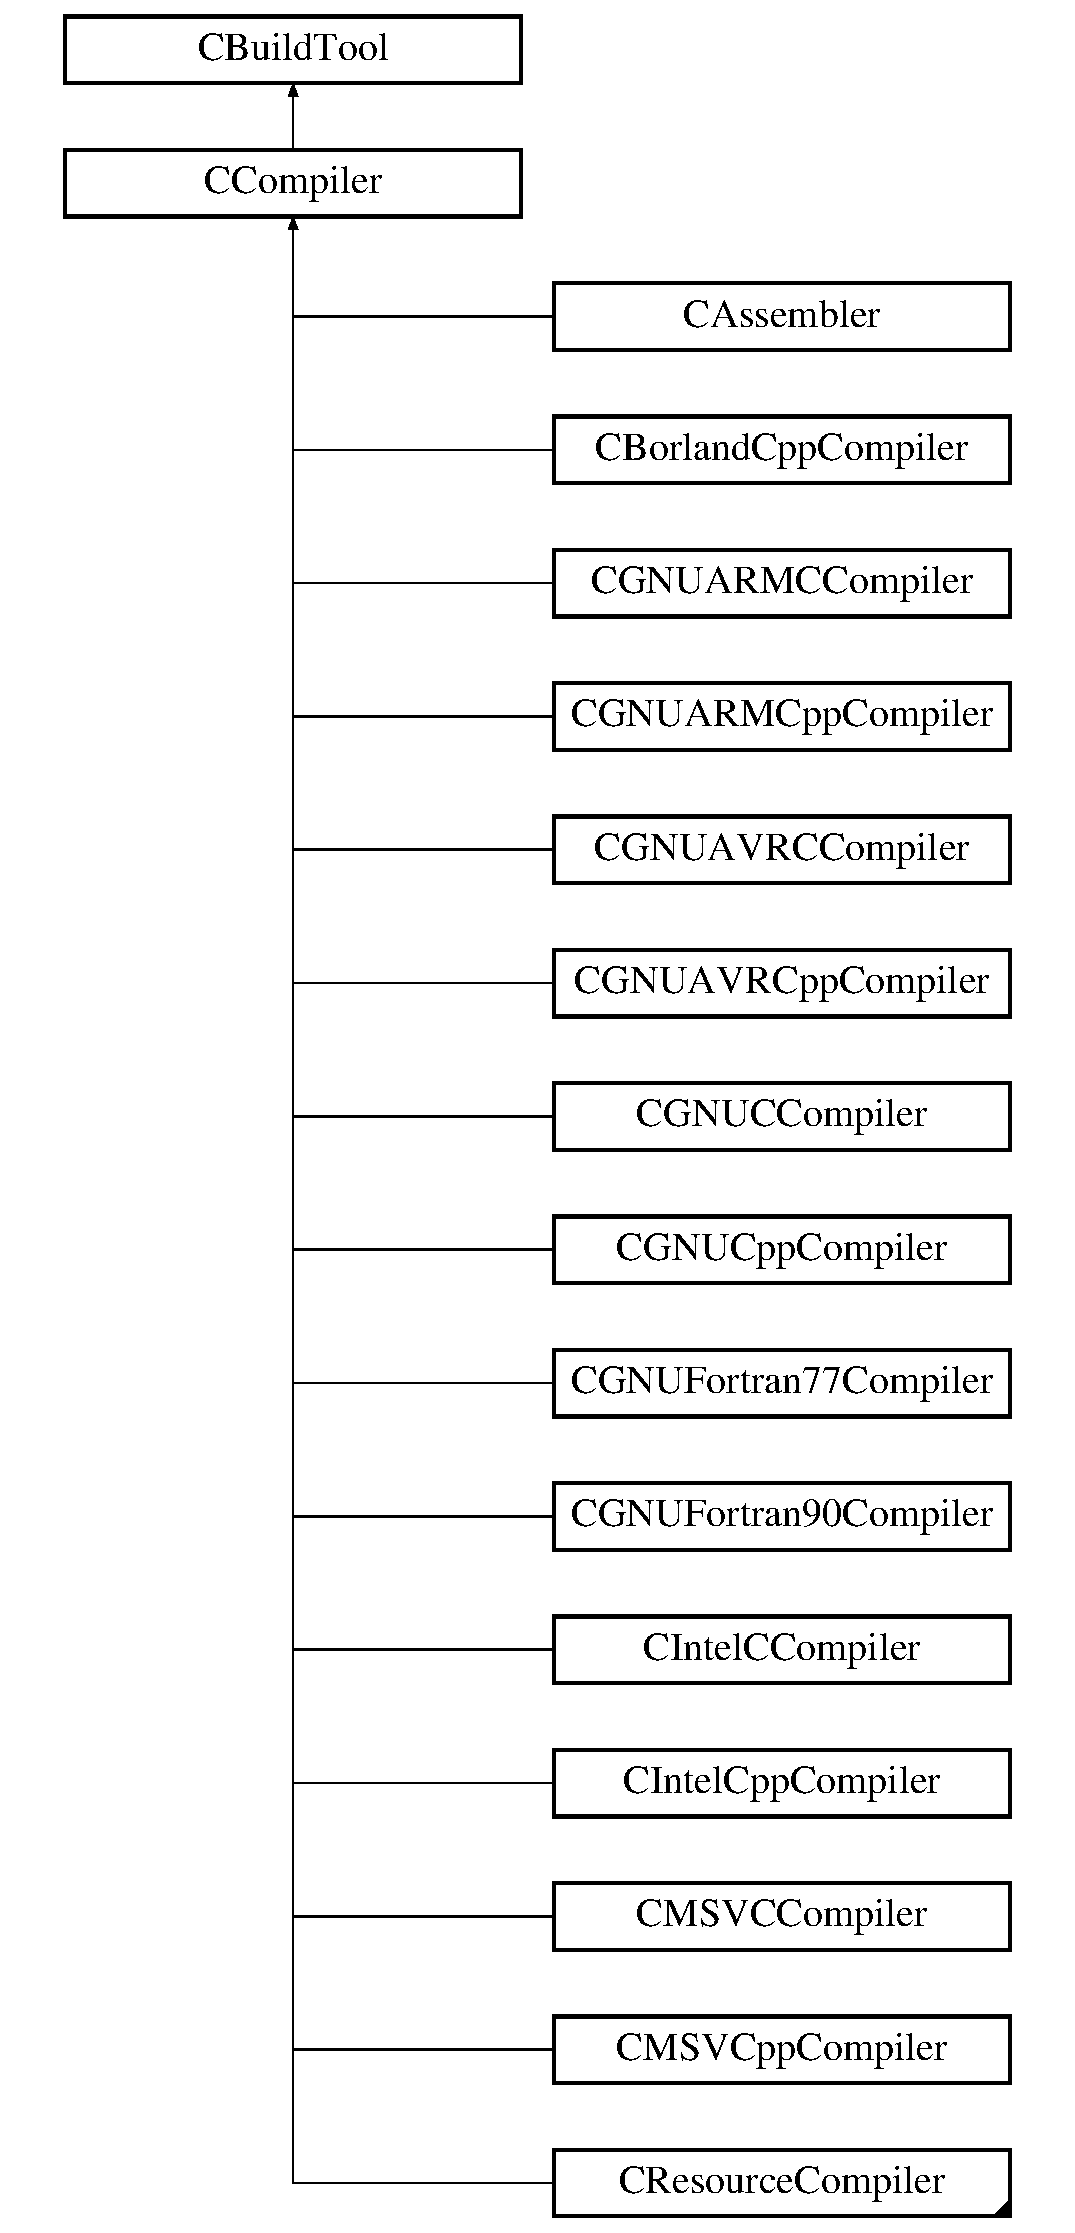
\includegraphics[height=12.000000cm]{d6/d5a/classCCompiler}
\end{center}
\end{figure}
\subsection*{Public Member Functions}
\begin{DoxyCompactItemize}
\item 
\hyperlink{classCString}{C\-String} \& \hyperlink{classCCompiler_a717ce85599a42b1477a3fce3a34459ba}{Include\-Dir\-Switch} (void)
\item 
\hyperlink{classCString}{C\-String} \& \hyperlink{classCCompiler_a3919ec93f4e95f23c617c3cc377a9201}{Define\-Switch} (void)
\item 
bool \& \hyperlink{classCCompiler_a8c93f10399942769018a0717bba38ea6}{Need\-Dependencies} (void)
\item 
virtual \hyperlink{classCIncludeSearchFilter}{C\-Include\-Search\-Filter} $\ast$ \hyperlink{classCCompiler_a1dc477f47e953ddd4c653f3ba85c5468}{Include\-Search\-Filter} (void) const 
\item 
virtual \hyperlink{classCCompiler}{C\-Compiler} $\ast$ \hyperlink{classCCompiler_a3d4aaaf69e1ba6070c729fd042d90012}{Create\-Instance} (void)
\item 
virtual void \hyperlink{classCCompiler_ac842b165479db817bb86d56367988b10}{Read} (const Ti\-Xml\-Element $\ast$Build\-Tool\-Root)
\item 
virtual void \hyperlink{classCCompiler_a25f64fb47c532b5261c44aca09b34cfa}{Write} (Ti\-Xml\-Element $\ast$Build\-Tool\-Root)
\item 
virtual void \hyperlink{classCCompiler_a07a1bbfb0fc606cf74bccc1ab64a64e8}{Show} (void)
\item 
\hyperlink{classCCompiler_ab6af9b8296df0390fc4b3d21374a0546}{C\-Compiler} (void)
\item 
\hyperlink{classCCompiler_acf3d4756541ce4cf3872de266313dc01}{C\-Compiler} (const \hyperlink{classCCompiler}{C\-Compiler} \&Compiler)
\item 
virtual \hyperlink{classCCompiler_ac305ef10b09c43a81f14389e482f07f8}{$\sim$\-C\-Compiler} (void)
\end{DoxyCompactItemize}
\subsection*{Protected Attributes}
\begin{DoxyCompactItemize}
\item 
\hyperlink{classCString}{C\-String} \hyperlink{classCCompiler_a68e5d39931d7dcaabe9fe019a3838ed4}{m\-\_\-\-Include\-Dir\-Switch}
\item 
\hyperlink{classCString}{C\-String} \hyperlink{classCCompiler_aec5b354b2fa305ca95696cb2fb7d8e79}{m\-\_\-\-Define\-Switch}
\item 
bool \hyperlink{classCCompiler_a8fb628e8ffdab42f6d562229e4e9d2ed}{m\-\_\-\-Need\-Dependencies}
\end{DoxyCompactItemize}
\subsection*{Additional Inherited Members}


\subsection{Constructor \& Destructor Documentation}
\hypertarget{classCCompiler_ab6af9b8296df0390fc4b3d21374a0546}{\index{C\-Compiler@{C\-Compiler}!C\-Compiler@{C\-Compiler}}
\index{C\-Compiler@{C\-Compiler}!CCompiler@{C\-Compiler}}
\subsubsection[{C\-Compiler}]{\setlength{\rightskip}{0pt plus 5cm}C\-Compiler\-::\-C\-Compiler (
\begin{DoxyParamCaption}
\item[{void}]{}
\end{DoxyParamCaption}
)}}\label{classCCompiler_ab6af9b8296df0390fc4b3d21374a0546}
\hypertarget{classCCompiler_acf3d4756541ce4cf3872de266313dc01}{\index{C\-Compiler@{C\-Compiler}!C\-Compiler@{C\-Compiler}}
\index{C\-Compiler@{C\-Compiler}!CCompiler@{C\-Compiler}}
\subsubsection[{C\-Compiler}]{\setlength{\rightskip}{0pt plus 5cm}C\-Compiler\-::\-C\-Compiler (
\begin{DoxyParamCaption}
\item[{const {\bf C\-Compiler} \&}]{Compiler}
\end{DoxyParamCaption}
)}}\label{classCCompiler_acf3d4756541ce4cf3872de266313dc01}
\hypertarget{classCCompiler_ac305ef10b09c43a81f14389e482f07f8}{\index{C\-Compiler@{C\-Compiler}!$\sim$\-C\-Compiler@{$\sim$\-C\-Compiler}}
\index{$\sim$\-C\-Compiler@{$\sim$\-C\-Compiler}!CCompiler@{C\-Compiler}}
\subsubsection[{$\sim$\-C\-Compiler}]{\setlength{\rightskip}{0pt plus 5cm}C\-Compiler\-::$\sim$\-C\-Compiler (
\begin{DoxyParamCaption}
\item[{void}]{}
\end{DoxyParamCaption}
)\hspace{0.3cm}{\ttfamily [virtual]}}}\label{classCCompiler_ac305ef10b09c43a81f14389e482f07f8}


\subsection{Member Function Documentation}
\hypertarget{classCCompiler_a3d4aaaf69e1ba6070c729fd042d90012}{\index{C\-Compiler@{C\-Compiler}!Create\-Instance@{Create\-Instance}}
\index{Create\-Instance@{Create\-Instance}!CCompiler@{C\-Compiler}}
\subsubsection[{Create\-Instance}]{\setlength{\rightskip}{0pt plus 5cm}{\bf C\-Compiler} $\ast$ C\-Compiler\-::\-Create\-Instance (
\begin{DoxyParamCaption}
\item[{void}]{}
\end{DoxyParamCaption}
)\hspace{0.3cm}{\ttfamily [virtual]}}}\label{classCCompiler_a3d4aaaf69e1ba6070c729fd042d90012}


Reimplemented from \hyperlink{classCBuildTool_aa7f0e7c0bd7f75c71d37df066bcb581e}{C\-Build\-Tool}.



Reimplemented in \hyperlink{classCMSVCResourceCompiler_aabd1683b76c181322754107af65ed8e0}{C\-M\-S\-V\-C\-Resource\-Compiler}, \hyperlink{classCMSVCppCompiler_ace8c0f315b83286474cdf8c8b41db75a}{C\-M\-S\-V\-Cpp\-Compiler}, \hyperlink{classCMSVCCompiler_a00dec77c231cace2f66fe45fccb25c7e}{C\-M\-S\-V\-C\-Compiler}, \hyperlink{classCIntelCppCompiler_a2e75b0ac5a7860128f25f29698f51509}{C\-Intel\-Cpp\-Compiler}, \hyperlink{classCIntelCCompiler_a4f259da4011feabc53b1ebf9a26bd2de}{C\-Intel\-C\-Compiler}, \hyperlink{classCBorlandResourceCompiler_a5c6aeef4fa07fb9693feb860a70729e0}{C\-Borland\-Resource\-Compiler}, \hyperlink{classCBorlandCppCompiler_a49178aa21245a1400f38c71631b7fa78}{C\-Borland\-Cpp\-Compiler}, \hyperlink{classCGNUARMWindowsResourceCompiler_a8da0eff0b561e69f2e2178965cd69253}{C\-G\-N\-U\-A\-R\-M\-Windows\-Resource\-Compiler}, \hyperlink{classCGNUARMCppCompiler_ae61a4db30f31a36bc46341da83ac9c63}{C\-G\-N\-U\-A\-R\-M\-Cpp\-Compiler}, \hyperlink{classCGNUARMCCompiler_a3e102dcc65d172a098282c5554e79302}{C\-G\-N\-U\-A\-R\-M\-C\-Compiler}, \hyperlink{classCGNUAVRCppCompiler_ac38cdc207e9dce42f53fef90ebaa3b87}{C\-G\-N\-U\-A\-V\-R\-Cpp\-Compiler}, \hyperlink{classCGNUAVRCCompiler_ad5630a463e0a41b5ecf28295f2c16e2f}{C\-G\-N\-U\-A\-V\-R\-C\-Compiler}, \hyperlink{classCGNUWindowsResourceCompiler_a295b322f12aa797537c0ef38bed0a9a5}{C\-G\-N\-U\-Windows\-Resource\-Compiler}, \hyperlink{classCGNUFortran90Compiler_a40bbc9c4d1417331e65990ed6f402d24}{C\-G\-N\-U\-Fortran90\-Compiler}, \hyperlink{classCGNUFortran77Compiler_ac9303b9366e63a08983cabcdfcb5cf06}{C\-G\-N\-U\-Fortran77\-Compiler}, \hyperlink{classCGNUCppCompiler_a0e6856b3906b6b32951f9796fba16316}{C\-G\-N\-U\-Cpp\-Compiler}, \hyperlink{classCGNUCCompiler_ae69827132a9bc1170f2073bf4ded88bc}{C\-G\-N\-U\-C\-Compiler}, \hyperlink{classCResourceCompiler_a4f46ae1558a0096b040eb593d28a810c}{C\-Resource\-Compiler}, and \hyperlink{classCAssembler_abc4ab373b93fc0980c204764afa73306}{C\-Assembler}.

\hypertarget{classCCompiler_a3919ec93f4e95f23c617c3cc377a9201}{\index{C\-Compiler@{C\-Compiler}!Define\-Switch@{Define\-Switch}}
\index{Define\-Switch@{Define\-Switch}!CCompiler@{C\-Compiler}}
\subsubsection[{Define\-Switch}]{\setlength{\rightskip}{0pt plus 5cm}{\bf C\-String}\& C\-Compiler\-::\-Define\-Switch (
\begin{DoxyParamCaption}
\item[{void}]{}
\end{DoxyParamCaption}
)\hspace{0.3cm}{\ttfamily [inline]}}}\label{classCCompiler_a3919ec93f4e95f23c617c3cc377a9201}
\hypertarget{classCCompiler_a717ce85599a42b1477a3fce3a34459ba}{\index{C\-Compiler@{C\-Compiler}!Include\-Dir\-Switch@{Include\-Dir\-Switch}}
\index{Include\-Dir\-Switch@{Include\-Dir\-Switch}!CCompiler@{C\-Compiler}}
\subsubsection[{Include\-Dir\-Switch}]{\setlength{\rightskip}{0pt plus 5cm}{\bf C\-String}\& C\-Compiler\-::\-Include\-Dir\-Switch (
\begin{DoxyParamCaption}
\item[{void}]{}
\end{DoxyParamCaption}
)\hspace{0.3cm}{\ttfamily [inline]}}}\label{classCCompiler_a717ce85599a42b1477a3fce3a34459ba}
\hypertarget{classCCompiler_a1dc477f47e953ddd4c653f3ba85c5468}{\index{C\-Compiler@{C\-Compiler}!Include\-Search\-Filter@{Include\-Search\-Filter}}
\index{Include\-Search\-Filter@{Include\-Search\-Filter}!CCompiler@{C\-Compiler}}
\subsubsection[{Include\-Search\-Filter}]{\setlength{\rightskip}{0pt plus 5cm}virtual {\bf C\-Include\-Search\-Filter}$\ast$ C\-Compiler\-::\-Include\-Search\-Filter (
\begin{DoxyParamCaption}
\item[{void}]{}
\end{DoxyParamCaption}
) const\hspace{0.3cm}{\ttfamily [inline]}, {\ttfamily [virtual]}}}\label{classCCompiler_a1dc477f47e953ddd4c653f3ba85c5468}


Reimplemented in \hyperlink{classCMSVCppCompiler_a67117b6e7c193f8d7357f32b868252cd}{C\-M\-S\-V\-Cpp\-Compiler}, \hyperlink{classCMSVCCompiler_a0ae941f148de8e1cbfefa8361034aeec}{C\-M\-S\-V\-C\-Compiler}, \hyperlink{classCIntelCppCompiler_a7937ce18c293da16161f14e51d873b5a}{C\-Intel\-Cpp\-Compiler}, \hyperlink{classCIntelCCompiler_a1864ae37aea1eecddfcec8ab456dc8a3}{C\-Intel\-C\-Compiler}, \hyperlink{classCBorlandCppCompiler_a9619772f500bb2f06d4a07349b08d05d}{C\-Borland\-Cpp\-Compiler}, \hyperlink{classCGNUARMCppCompiler_a061d65ad921d3856be6e2b8f80976106}{C\-G\-N\-U\-A\-R\-M\-Cpp\-Compiler}, \hyperlink{classCGNUARMCCompiler_a455c9c55a802d6a2e7e6d5146e252554}{C\-G\-N\-U\-A\-R\-M\-C\-Compiler}, \hyperlink{classCGNUAVRCppCompiler_aae41e83908ef6be8ae274f75fb6a1cbe}{C\-G\-N\-U\-A\-V\-R\-Cpp\-Compiler}, \hyperlink{classCGNUAVRCCompiler_a278ccc28910fb9cb8a20587bd966cf55}{C\-G\-N\-U\-A\-V\-R\-C\-Compiler}, \hyperlink{classCGNUCppCompiler_a70e0a0d27cded35b66807d8e2804ade8}{C\-G\-N\-U\-Cpp\-Compiler}, and \hyperlink{classCGNUCCompiler_a1dc37484a88684465d9bbfed8ee335e2}{C\-G\-N\-U\-C\-Compiler}.

\hypertarget{classCCompiler_a8c93f10399942769018a0717bba38ea6}{\index{C\-Compiler@{C\-Compiler}!Need\-Dependencies@{Need\-Dependencies}}
\index{Need\-Dependencies@{Need\-Dependencies}!CCompiler@{C\-Compiler}}
\subsubsection[{Need\-Dependencies}]{\setlength{\rightskip}{0pt plus 5cm}bool\& C\-Compiler\-::\-Need\-Dependencies (
\begin{DoxyParamCaption}
\item[{void}]{}
\end{DoxyParamCaption}
)\hspace{0.3cm}{\ttfamily [inline]}}}\label{classCCompiler_a8c93f10399942769018a0717bba38ea6}
\hypertarget{classCCompiler_ac842b165479db817bb86d56367988b10}{\index{C\-Compiler@{C\-Compiler}!Read@{Read}}
\index{Read@{Read}!CCompiler@{C\-Compiler}}
\subsubsection[{Read}]{\setlength{\rightskip}{0pt plus 5cm}void C\-Compiler\-::\-Read (
\begin{DoxyParamCaption}
\item[{const Ti\-Xml\-Element $\ast$}]{Build\-Tool\-Root}
\end{DoxyParamCaption}
)\hspace{0.3cm}{\ttfamily [virtual]}}}\label{classCCompiler_ac842b165479db817bb86d56367988b10}


Reimplemented from \hyperlink{classCBuildTool_a299d87943c0f68dde5316318cc0838f8}{C\-Build\-Tool}.

\hypertarget{classCCompiler_a07a1bbfb0fc606cf74bccc1ab64a64e8}{\index{C\-Compiler@{C\-Compiler}!Show@{Show}}
\index{Show@{Show}!CCompiler@{C\-Compiler}}
\subsubsection[{Show}]{\setlength{\rightskip}{0pt plus 5cm}void C\-Compiler\-::\-Show (
\begin{DoxyParamCaption}
\item[{void}]{}
\end{DoxyParamCaption}
)\hspace{0.3cm}{\ttfamily [virtual]}}}\label{classCCompiler_a07a1bbfb0fc606cf74bccc1ab64a64e8}


Reimplemented from \hyperlink{classCBuildTool_a69815d1393a61dc16b2cc2d0552cd5ac}{C\-Build\-Tool}.

\hypertarget{classCCompiler_a25f64fb47c532b5261c44aca09b34cfa}{\index{C\-Compiler@{C\-Compiler}!Write@{Write}}
\index{Write@{Write}!CCompiler@{C\-Compiler}}
\subsubsection[{Write}]{\setlength{\rightskip}{0pt plus 5cm}void C\-Compiler\-::\-Write (
\begin{DoxyParamCaption}
\item[{Ti\-Xml\-Element $\ast$}]{Build\-Tool\-Root}
\end{DoxyParamCaption}
)\hspace{0.3cm}{\ttfamily [virtual]}}}\label{classCCompiler_a25f64fb47c532b5261c44aca09b34cfa}


Reimplemented from \hyperlink{classCBuildTool_af0331a777785bc2d15236b5c74321ed2}{C\-Build\-Tool}.



\subsection{Member Data Documentation}
\hypertarget{classCCompiler_aec5b354b2fa305ca95696cb2fb7d8e79}{\index{C\-Compiler@{C\-Compiler}!m\-\_\-\-Define\-Switch@{m\-\_\-\-Define\-Switch}}
\index{m\-\_\-\-Define\-Switch@{m\-\_\-\-Define\-Switch}!CCompiler@{C\-Compiler}}
\subsubsection[{m\-\_\-\-Define\-Switch}]{\setlength{\rightskip}{0pt plus 5cm}{\bf C\-String} C\-Compiler\-::m\-\_\-\-Define\-Switch\hspace{0.3cm}{\ttfamily [protected]}}}\label{classCCompiler_aec5b354b2fa305ca95696cb2fb7d8e79}
\hypertarget{classCCompiler_a68e5d39931d7dcaabe9fe019a3838ed4}{\index{C\-Compiler@{C\-Compiler}!m\-\_\-\-Include\-Dir\-Switch@{m\-\_\-\-Include\-Dir\-Switch}}
\index{m\-\_\-\-Include\-Dir\-Switch@{m\-\_\-\-Include\-Dir\-Switch}!CCompiler@{C\-Compiler}}
\subsubsection[{m\-\_\-\-Include\-Dir\-Switch}]{\setlength{\rightskip}{0pt plus 5cm}{\bf C\-String} C\-Compiler\-::m\-\_\-\-Include\-Dir\-Switch\hspace{0.3cm}{\ttfamily [protected]}}}\label{classCCompiler_a68e5d39931d7dcaabe9fe019a3838ed4}
\hypertarget{classCCompiler_a8fb628e8ffdab42f6d562229e4e9d2ed}{\index{C\-Compiler@{C\-Compiler}!m\-\_\-\-Need\-Dependencies@{m\-\_\-\-Need\-Dependencies}}
\index{m\-\_\-\-Need\-Dependencies@{m\-\_\-\-Need\-Dependencies}!CCompiler@{C\-Compiler}}
\subsubsection[{m\-\_\-\-Need\-Dependencies}]{\setlength{\rightskip}{0pt plus 5cm}bool C\-Compiler\-::m\-\_\-\-Need\-Dependencies\hspace{0.3cm}{\ttfamily [protected]}}}\label{classCCompiler_a8fb628e8ffdab42f6d562229e4e9d2ed}


The documentation for this class was generated from the following files\-:\begin{DoxyCompactItemize}
\item 
src/\hyperlink{buildtools_8h}{buildtools.\-h}\item 
src/\hyperlink{buildtools_8cpp}{buildtools.\-cpp}\end{DoxyCompactItemize}

\hypertarget{classCConfiguration}{\section{C\-Configuration Class Reference}
\label{classCConfiguration}\index{C\-Configuration@{C\-Configuration}}
}


{\ttfamily \#include $<$stlconfig.\-h$>$}

Inheritance diagram for C\-Configuration\-:\begin{figure}[H]
\begin{center}
\leavevmode
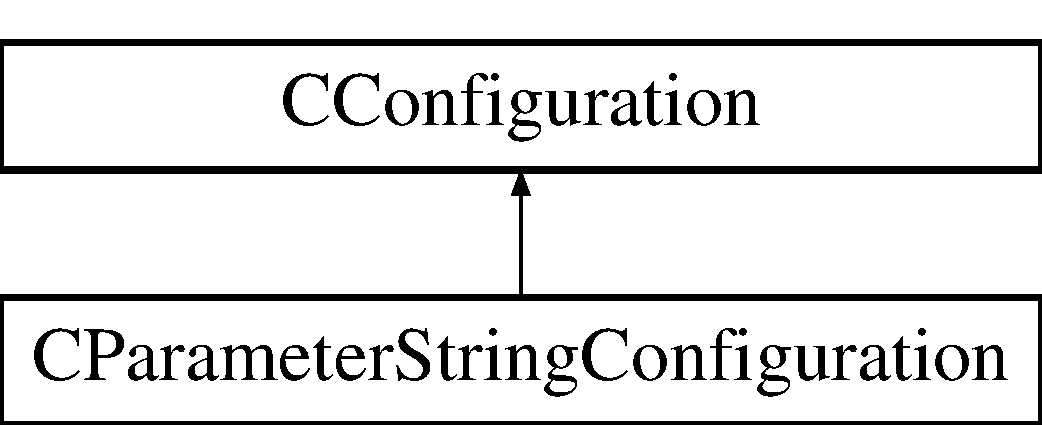
\includegraphics[height=2.000000cm]{dc/d01/classCConfiguration}
\end{center}
\end{figure}
\subsection*{Public Member Functions}
\begin{DoxyCompactItemize}
\item 
virtual void \hyperlink{classCConfiguration_a20cb2322663278d521175a1938407e71}{Initialize} (void)
\item 
virtual void \hyperlink{classCConfiguration_abb885f482171f99631785dc3d0685aab}{Clear} (void)
\item 
int \hyperlink{classCConfiguration_a9049c49228af7c7a6e12882f8e7356f4}{Get\-Count} (void) const 
\item 
\hyperlink{classCString}{C\-String} \& \hyperlink{classCConfiguration_ae083d99364629d6c45698449b0d39ee6}{Defined\-Prefix} (void)
\item 
\hyperlink{classCString}{C\-String} \hyperlink{classCConfiguration_aec3c760ef7a7f5571a2489dfdac47b69}{Defined\-Prefix} (void) const 
\item 
bool \hyperlink{classCConfiguration_a2bd48a783d6a2c0a71e74dfab84211df}{Var\-Defined} (const \hyperlink{classCString}{C\-String} \&Name) const 
\item 
void \hyperlink{classCConfiguration_a5ca7d9dd9858099936ff9b581a7ab79b}{Set\-Defined} (const \hyperlink{classCString}{C\-String} \&Name)
\item 
void \hyperlink{classCConfiguration_a2e9b2e96b342d8f3c8c2ae06e0f80019}{Set\-Undefined} (const \hyperlink{classCString}{C\-String} \&Name)
\item 
\hyperlink{classCVariable}{C\-Variable} \& \hyperlink{classCConfiguration_a9983c5dd69ea4fe163c7043381e1da52}{Variable} (const int Index)
\item 
\hyperlink{classCVariable}{C\-Variable} \& \hyperlink{classCConfiguration_a0f6e583cbf9d17f864efa3d982730a55}{Var\-Named} (const \hyperlink{classCString}{C\-String} \&Name)
\item 
int \hyperlink{classCConfiguration_a2c1cace09788549acc212cd10f822b31}{Var\-Index} (const \hyperlink{classCString}{C\-String} \&Name) const 
\item 
int \hyperlink{classCConfiguration_a34ca50d4c0c92cbe032abd2e53804de3}{Insert\-Integer\-Variable} (const \hyperlink{classCString}{C\-String} \&Name, const int Value=0)
\item 
int \hyperlink{classCConfiguration_a998e32d3c6cddecf064e020748cbe331}{Insert\-Float\-Variable} (const \hyperlink{classCString}{C\-String} \&Name, const double Value=0.\-0)
\item 
int \hyperlink{classCConfiguration_a30ee323a4668bacd38bbed0d11192f55}{Insert\-Boolean\-Variable} (const \hyperlink{classCString}{C\-String} \&Name, const bool Value=false)
\item 
int \hyperlink{classCConfiguration_aa0006435e2b8a4c5a72ef3d5a0a8849b}{Insert\-String\-Variable} (const \hyperlink{classCString}{C\-String} \&Name, const \hyperlink{classCString}{C\-String} \&Value=\char`\"{}\char`\"{})
\item 
int \hyperlink{classCConfiguration_a2f3e36f9ec1d6ab3076ab46501136bf4}{Insert\-Char\-Variable} (const \hyperlink{classCString}{C\-String} \&Name, const char Value=char(0))
\item 
void \hyperlink{classCConfiguration_aa71a97f192c38fa37df1ad75a7789460}{Remove\-Variable} (const int Index)
\item 
void \hyperlink{classCConfiguration_a2b4c8069b424baabc7eb15b6c91349eb}{Remove\-Variable} (const \hyperlink{classCString}{C\-String} \&Name)
\item 
void \hyperlink{classCConfiguration_a2f69b4e64ee22d43f50d37644cb36c7b}{Set\-Integer\-Variable} (const \hyperlink{classCString}{C\-String} \&Name, const int Value)
\item 
void \hyperlink{classCConfiguration_a18bb6f1546cb662a1cf4bec4deb587ba}{Set\-Float\-Variable} (const \hyperlink{classCString}{C\-String} \&Name, const double Value)
\item 
void \hyperlink{classCConfiguration_a4d9a58e5376e4dc66c72c2b2713cfb31}{Set\-Boolean\-Variable} (const \hyperlink{classCString}{C\-String} \&Name, const bool Value)
\item 
void \hyperlink{classCConfiguration_a37ea2a42c36bcef95fddc28fdd4ac34b}{Set\-String\-Variable} (const \hyperlink{classCString}{C\-String} \&Name, const \hyperlink{classCString}{C\-String} \&Value)
\item 
void \hyperlink{classCConfiguration_a78acb5cc352d63460876b91622d976cc}{Set\-Char\-Variable} (const \hyperlink{classCString}{C\-String} \&Name, const char Value)
\item 
void \hyperlink{classCConfiguration_ad7567abe3549c11531f1b3c599990230}{Print} (std\-::ostream \&out)
\item 
void \hyperlink{classCConfiguration_a9bd44bd2a143aea3b794294f4c12ac7a}{Process\-Parameters} (int argc, char $\ast$argv\mbox{[}$\,$\mbox{]})
\item 
void \hyperlink{classCConfiguration_a18a27bc8369914d3fdb924fb44c63fff}{Load\-From\-File} (const \hyperlink{classCString}{C\-String} \&File\-Name)
\item 
void \hyperlink{classCConfiguration_ad379e27380475b31348f95f04db75257}{Save\-To\-File} (const \hyperlink{classCString}{C\-String} \&File\-Name)
\item 
\hyperlink{classCConfiguration_adc320be38da481ec9c33b02777991425}{C\-Configuration} (void)
\item 
virtual \hyperlink{classCConfiguration_a64473225d29e05323df79c0f17799d8b}{$\sim$\-C\-Configuration} (void)
\end{DoxyCompactItemize}
\subsection*{Protected Member Functions}
\begin{DoxyCompactItemize}
\item 
bool \hyperlink{classCConfiguration_a0015975c9f3c3ef92c10d10024fb9312}{Valid\-Index} (const int Index) const 
\end{DoxyCompactItemize}
\subsection*{Protected Attributes}
\begin{DoxyCompactItemize}
\item 
\hyperlink{classCVariable}{C\-Variable} \hyperlink{classCConfiguration_a3e379beeb1a6795eaf95740a0054f215}{m\-\_\-\-Null\-Variable}
\item 
std\-::vector$<$ \hyperlink{classCVariable}{C\-Variable} $\ast$ $>$ \hyperlink{classCConfiguration_ab55474edc9916f3e057ca0019be734c2}{m\-\_\-\-Variables}
\item 
\hyperlink{classCString}{C\-String} \hyperlink{classCConfiguration_a85333335417a9d19030b03273562adee}{m\-\_\-\-Defined\-Prefix}
\end{DoxyCompactItemize}


\subsection{Constructor \& Destructor Documentation}
\hypertarget{classCConfiguration_adc320be38da481ec9c33b02777991425}{\index{C\-Configuration@{C\-Configuration}!C\-Configuration@{C\-Configuration}}
\index{C\-Configuration@{C\-Configuration}!CConfiguration@{C\-Configuration}}
\subsubsection[{C\-Configuration}]{\setlength{\rightskip}{0pt plus 5cm}C\-Configuration\-::\-C\-Configuration (
\begin{DoxyParamCaption}
\item[{void}]{}
\end{DoxyParamCaption}
)}}\label{classCConfiguration_adc320be38da481ec9c33b02777991425}
\hypertarget{classCConfiguration_a64473225d29e05323df79c0f17799d8b}{\index{C\-Configuration@{C\-Configuration}!$\sim$\-C\-Configuration@{$\sim$\-C\-Configuration}}
\index{$\sim$\-C\-Configuration@{$\sim$\-C\-Configuration}!CConfiguration@{C\-Configuration}}
\subsubsection[{$\sim$\-C\-Configuration}]{\setlength{\rightskip}{0pt plus 5cm}C\-Configuration\-::$\sim$\-C\-Configuration (
\begin{DoxyParamCaption}
\item[{void}]{}
\end{DoxyParamCaption}
)\hspace{0.3cm}{\ttfamily [virtual]}}}\label{classCConfiguration_a64473225d29e05323df79c0f17799d8b}


\subsection{Member Function Documentation}
\hypertarget{classCConfiguration_abb885f482171f99631785dc3d0685aab}{\index{C\-Configuration@{C\-Configuration}!Clear@{Clear}}
\index{Clear@{Clear}!CConfiguration@{C\-Configuration}}
\subsubsection[{Clear}]{\setlength{\rightskip}{0pt plus 5cm}void C\-Configuration\-::\-Clear (
\begin{DoxyParamCaption}
\item[{void}]{}
\end{DoxyParamCaption}
)\hspace{0.3cm}{\ttfamily [virtual]}}}\label{classCConfiguration_abb885f482171f99631785dc3d0685aab}
\hypertarget{classCConfiguration_ae083d99364629d6c45698449b0d39ee6}{\index{C\-Configuration@{C\-Configuration}!Defined\-Prefix@{Defined\-Prefix}}
\index{Defined\-Prefix@{Defined\-Prefix}!CConfiguration@{C\-Configuration}}
\subsubsection[{Defined\-Prefix}]{\setlength{\rightskip}{0pt plus 5cm}{\bf C\-String}\& C\-Configuration\-::\-Defined\-Prefix (
\begin{DoxyParamCaption}
\item[{void}]{}
\end{DoxyParamCaption}
)\hspace{0.3cm}{\ttfamily [inline]}}}\label{classCConfiguration_ae083d99364629d6c45698449b0d39ee6}
\hypertarget{classCConfiguration_aec3c760ef7a7f5571a2489dfdac47b69}{\index{C\-Configuration@{C\-Configuration}!Defined\-Prefix@{Defined\-Prefix}}
\index{Defined\-Prefix@{Defined\-Prefix}!CConfiguration@{C\-Configuration}}
\subsubsection[{Defined\-Prefix}]{\setlength{\rightskip}{0pt plus 5cm}{\bf C\-String} C\-Configuration\-::\-Defined\-Prefix (
\begin{DoxyParamCaption}
\item[{void}]{}
\end{DoxyParamCaption}
) const\hspace{0.3cm}{\ttfamily [inline]}}}\label{classCConfiguration_aec3c760ef7a7f5571a2489dfdac47b69}
\hypertarget{classCConfiguration_a9049c49228af7c7a6e12882f8e7356f4}{\index{C\-Configuration@{C\-Configuration}!Get\-Count@{Get\-Count}}
\index{Get\-Count@{Get\-Count}!CConfiguration@{C\-Configuration}}
\subsubsection[{Get\-Count}]{\setlength{\rightskip}{0pt plus 5cm}int C\-Configuration\-::\-Get\-Count (
\begin{DoxyParamCaption}
\item[{void}]{}
\end{DoxyParamCaption}
) const}}\label{classCConfiguration_a9049c49228af7c7a6e12882f8e7356f4}
\hypertarget{classCConfiguration_a20cb2322663278d521175a1938407e71}{\index{C\-Configuration@{C\-Configuration}!Initialize@{Initialize}}
\index{Initialize@{Initialize}!CConfiguration@{C\-Configuration}}
\subsubsection[{Initialize}]{\setlength{\rightskip}{0pt plus 5cm}virtual void C\-Configuration\-::\-Initialize (
\begin{DoxyParamCaption}
\item[{void}]{}
\end{DoxyParamCaption}
)\hspace{0.3cm}{\ttfamily [inline]}, {\ttfamily [virtual]}}}\label{classCConfiguration_a20cb2322663278d521175a1938407e71}
\hypertarget{classCConfiguration_a30ee323a4668bacd38bbed0d11192f55}{\index{C\-Configuration@{C\-Configuration}!Insert\-Boolean\-Variable@{Insert\-Boolean\-Variable}}
\index{Insert\-Boolean\-Variable@{Insert\-Boolean\-Variable}!CConfiguration@{C\-Configuration}}
\subsubsection[{Insert\-Boolean\-Variable}]{\setlength{\rightskip}{0pt plus 5cm}int C\-Configuration\-::\-Insert\-Boolean\-Variable (
\begin{DoxyParamCaption}
\item[{const {\bf C\-String} \&}]{Name, }
\item[{const bool}]{Value = {\ttfamily false}}
\end{DoxyParamCaption}
)}}\label{classCConfiguration_a30ee323a4668bacd38bbed0d11192f55}
\hypertarget{classCConfiguration_a2f3e36f9ec1d6ab3076ab46501136bf4}{\index{C\-Configuration@{C\-Configuration}!Insert\-Char\-Variable@{Insert\-Char\-Variable}}
\index{Insert\-Char\-Variable@{Insert\-Char\-Variable}!CConfiguration@{C\-Configuration}}
\subsubsection[{Insert\-Char\-Variable}]{\setlength{\rightskip}{0pt plus 5cm}int C\-Configuration\-::\-Insert\-Char\-Variable (
\begin{DoxyParamCaption}
\item[{const {\bf C\-String} \&}]{Name, }
\item[{const char}]{Value = {\ttfamily char(0)}}
\end{DoxyParamCaption}
)}}\label{classCConfiguration_a2f3e36f9ec1d6ab3076ab46501136bf4}
\hypertarget{classCConfiguration_a998e32d3c6cddecf064e020748cbe331}{\index{C\-Configuration@{C\-Configuration}!Insert\-Float\-Variable@{Insert\-Float\-Variable}}
\index{Insert\-Float\-Variable@{Insert\-Float\-Variable}!CConfiguration@{C\-Configuration}}
\subsubsection[{Insert\-Float\-Variable}]{\setlength{\rightskip}{0pt plus 5cm}int C\-Configuration\-::\-Insert\-Float\-Variable (
\begin{DoxyParamCaption}
\item[{const {\bf C\-String} \&}]{Name, }
\item[{const double}]{Value = {\ttfamily 0.0}}
\end{DoxyParamCaption}
)}}\label{classCConfiguration_a998e32d3c6cddecf064e020748cbe331}
\hypertarget{classCConfiguration_a34ca50d4c0c92cbe032abd2e53804de3}{\index{C\-Configuration@{C\-Configuration}!Insert\-Integer\-Variable@{Insert\-Integer\-Variable}}
\index{Insert\-Integer\-Variable@{Insert\-Integer\-Variable}!CConfiguration@{C\-Configuration}}
\subsubsection[{Insert\-Integer\-Variable}]{\setlength{\rightskip}{0pt plus 5cm}int C\-Configuration\-::\-Insert\-Integer\-Variable (
\begin{DoxyParamCaption}
\item[{const {\bf C\-String} \&}]{Name, }
\item[{const int}]{Value = {\ttfamily 0}}
\end{DoxyParamCaption}
)}}\label{classCConfiguration_a34ca50d4c0c92cbe032abd2e53804de3}
\hypertarget{classCConfiguration_aa0006435e2b8a4c5a72ef3d5a0a8849b}{\index{C\-Configuration@{C\-Configuration}!Insert\-String\-Variable@{Insert\-String\-Variable}}
\index{Insert\-String\-Variable@{Insert\-String\-Variable}!CConfiguration@{C\-Configuration}}
\subsubsection[{Insert\-String\-Variable}]{\setlength{\rightskip}{0pt plus 5cm}int C\-Configuration\-::\-Insert\-String\-Variable (
\begin{DoxyParamCaption}
\item[{const {\bf C\-String} \&}]{Name, }
\item[{const {\bf C\-String} \&}]{Value = {\ttfamily \char`\"{}\char`\"{}}}
\end{DoxyParamCaption}
)}}\label{classCConfiguration_aa0006435e2b8a4c5a72ef3d5a0a8849b}
\hypertarget{classCConfiguration_a18a27bc8369914d3fdb924fb44c63fff}{\index{C\-Configuration@{C\-Configuration}!Load\-From\-File@{Load\-From\-File}}
\index{Load\-From\-File@{Load\-From\-File}!CConfiguration@{C\-Configuration}}
\subsubsection[{Load\-From\-File}]{\setlength{\rightskip}{0pt plus 5cm}void C\-Configuration\-::\-Load\-From\-File (
\begin{DoxyParamCaption}
\item[{const {\bf C\-String} \&}]{File\-Name}
\end{DoxyParamCaption}
)}}\label{classCConfiguration_a18a27bc8369914d3fdb924fb44c63fff}
\hypertarget{classCConfiguration_ad7567abe3549c11531f1b3c599990230}{\index{C\-Configuration@{C\-Configuration}!Print@{Print}}
\index{Print@{Print}!CConfiguration@{C\-Configuration}}
\subsubsection[{Print}]{\setlength{\rightskip}{0pt plus 5cm}void C\-Configuration\-::\-Print (
\begin{DoxyParamCaption}
\item[{std\-::ostream \&}]{out}
\end{DoxyParamCaption}
)}}\label{classCConfiguration_ad7567abe3549c11531f1b3c599990230}
\hypertarget{classCConfiguration_a9bd44bd2a143aea3b794294f4c12ac7a}{\index{C\-Configuration@{C\-Configuration}!Process\-Parameters@{Process\-Parameters}}
\index{Process\-Parameters@{Process\-Parameters}!CConfiguration@{C\-Configuration}}
\subsubsection[{Process\-Parameters}]{\setlength{\rightskip}{0pt plus 5cm}void C\-Configuration\-::\-Process\-Parameters (
\begin{DoxyParamCaption}
\item[{int}]{argc, }
\item[{char $\ast$}]{argv\mbox{[}$\,$\mbox{]}}
\end{DoxyParamCaption}
)}}\label{classCConfiguration_a9bd44bd2a143aea3b794294f4c12ac7a}
\hypertarget{classCConfiguration_aa71a97f192c38fa37df1ad75a7789460}{\index{C\-Configuration@{C\-Configuration}!Remove\-Variable@{Remove\-Variable}}
\index{Remove\-Variable@{Remove\-Variable}!CConfiguration@{C\-Configuration}}
\subsubsection[{Remove\-Variable}]{\setlength{\rightskip}{0pt plus 5cm}void C\-Configuration\-::\-Remove\-Variable (
\begin{DoxyParamCaption}
\item[{const int}]{Index}
\end{DoxyParamCaption}
)}}\label{classCConfiguration_aa71a97f192c38fa37df1ad75a7789460}
\hypertarget{classCConfiguration_a2b4c8069b424baabc7eb15b6c91349eb}{\index{C\-Configuration@{C\-Configuration}!Remove\-Variable@{Remove\-Variable}}
\index{Remove\-Variable@{Remove\-Variable}!CConfiguration@{C\-Configuration}}
\subsubsection[{Remove\-Variable}]{\setlength{\rightskip}{0pt plus 5cm}void C\-Configuration\-::\-Remove\-Variable (
\begin{DoxyParamCaption}
\item[{const {\bf C\-String} \&}]{Name}
\end{DoxyParamCaption}
)}}\label{classCConfiguration_a2b4c8069b424baabc7eb15b6c91349eb}
\hypertarget{classCConfiguration_ad379e27380475b31348f95f04db75257}{\index{C\-Configuration@{C\-Configuration}!Save\-To\-File@{Save\-To\-File}}
\index{Save\-To\-File@{Save\-To\-File}!CConfiguration@{C\-Configuration}}
\subsubsection[{Save\-To\-File}]{\setlength{\rightskip}{0pt plus 5cm}void C\-Configuration\-::\-Save\-To\-File (
\begin{DoxyParamCaption}
\item[{const {\bf C\-String} \&}]{File\-Name}
\end{DoxyParamCaption}
)}}\label{classCConfiguration_ad379e27380475b31348f95f04db75257}
\hypertarget{classCConfiguration_a4d9a58e5376e4dc66c72c2b2713cfb31}{\index{C\-Configuration@{C\-Configuration}!Set\-Boolean\-Variable@{Set\-Boolean\-Variable}}
\index{Set\-Boolean\-Variable@{Set\-Boolean\-Variable}!CConfiguration@{C\-Configuration}}
\subsubsection[{Set\-Boolean\-Variable}]{\setlength{\rightskip}{0pt plus 5cm}void C\-Configuration\-::\-Set\-Boolean\-Variable (
\begin{DoxyParamCaption}
\item[{const {\bf C\-String} \&}]{Name, }
\item[{const bool}]{Value}
\end{DoxyParamCaption}
)}}\label{classCConfiguration_a4d9a58e5376e4dc66c72c2b2713cfb31}
\hypertarget{classCConfiguration_a78acb5cc352d63460876b91622d976cc}{\index{C\-Configuration@{C\-Configuration}!Set\-Char\-Variable@{Set\-Char\-Variable}}
\index{Set\-Char\-Variable@{Set\-Char\-Variable}!CConfiguration@{C\-Configuration}}
\subsubsection[{Set\-Char\-Variable}]{\setlength{\rightskip}{0pt plus 5cm}void C\-Configuration\-::\-Set\-Char\-Variable (
\begin{DoxyParamCaption}
\item[{const {\bf C\-String} \&}]{Name, }
\item[{const char}]{Value}
\end{DoxyParamCaption}
)}}\label{classCConfiguration_a78acb5cc352d63460876b91622d976cc}
\hypertarget{classCConfiguration_a5ca7d9dd9858099936ff9b581a7ab79b}{\index{C\-Configuration@{C\-Configuration}!Set\-Defined@{Set\-Defined}}
\index{Set\-Defined@{Set\-Defined}!CConfiguration@{C\-Configuration}}
\subsubsection[{Set\-Defined}]{\setlength{\rightskip}{0pt plus 5cm}void C\-Configuration\-::\-Set\-Defined (
\begin{DoxyParamCaption}
\item[{const {\bf C\-String} \&}]{Name}
\end{DoxyParamCaption}
)}}\label{classCConfiguration_a5ca7d9dd9858099936ff9b581a7ab79b}
\hypertarget{classCConfiguration_a18bb6f1546cb662a1cf4bec4deb587ba}{\index{C\-Configuration@{C\-Configuration}!Set\-Float\-Variable@{Set\-Float\-Variable}}
\index{Set\-Float\-Variable@{Set\-Float\-Variable}!CConfiguration@{C\-Configuration}}
\subsubsection[{Set\-Float\-Variable}]{\setlength{\rightskip}{0pt plus 5cm}void C\-Configuration\-::\-Set\-Float\-Variable (
\begin{DoxyParamCaption}
\item[{const {\bf C\-String} \&}]{Name, }
\item[{const double}]{Value}
\end{DoxyParamCaption}
)}}\label{classCConfiguration_a18bb6f1546cb662a1cf4bec4deb587ba}
\hypertarget{classCConfiguration_a2f69b4e64ee22d43f50d37644cb36c7b}{\index{C\-Configuration@{C\-Configuration}!Set\-Integer\-Variable@{Set\-Integer\-Variable}}
\index{Set\-Integer\-Variable@{Set\-Integer\-Variable}!CConfiguration@{C\-Configuration}}
\subsubsection[{Set\-Integer\-Variable}]{\setlength{\rightskip}{0pt plus 5cm}void C\-Configuration\-::\-Set\-Integer\-Variable (
\begin{DoxyParamCaption}
\item[{const {\bf C\-String} \&}]{Name, }
\item[{const int}]{Value}
\end{DoxyParamCaption}
)}}\label{classCConfiguration_a2f69b4e64ee22d43f50d37644cb36c7b}
\hypertarget{classCConfiguration_a37ea2a42c36bcef95fddc28fdd4ac34b}{\index{C\-Configuration@{C\-Configuration}!Set\-String\-Variable@{Set\-String\-Variable}}
\index{Set\-String\-Variable@{Set\-String\-Variable}!CConfiguration@{C\-Configuration}}
\subsubsection[{Set\-String\-Variable}]{\setlength{\rightskip}{0pt plus 5cm}void C\-Configuration\-::\-Set\-String\-Variable (
\begin{DoxyParamCaption}
\item[{const {\bf C\-String} \&}]{Name, }
\item[{const {\bf C\-String} \&}]{Value}
\end{DoxyParamCaption}
)}}\label{classCConfiguration_a37ea2a42c36bcef95fddc28fdd4ac34b}
\hypertarget{classCConfiguration_a2e9b2e96b342d8f3c8c2ae06e0f80019}{\index{C\-Configuration@{C\-Configuration}!Set\-Undefined@{Set\-Undefined}}
\index{Set\-Undefined@{Set\-Undefined}!CConfiguration@{C\-Configuration}}
\subsubsection[{Set\-Undefined}]{\setlength{\rightskip}{0pt plus 5cm}void C\-Configuration\-::\-Set\-Undefined (
\begin{DoxyParamCaption}
\item[{const {\bf C\-String} \&}]{Name}
\end{DoxyParamCaption}
)}}\label{classCConfiguration_a2e9b2e96b342d8f3c8c2ae06e0f80019}
\hypertarget{classCConfiguration_a0015975c9f3c3ef92c10d10024fb9312}{\index{C\-Configuration@{C\-Configuration}!Valid\-Index@{Valid\-Index}}
\index{Valid\-Index@{Valid\-Index}!CConfiguration@{C\-Configuration}}
\subsubsection[{Valid\-Index}]{\setlength{\rightskip}{0pt plus 5cm}bool C\-Configuration\-::\-Valid\-Index (
\begin{DoxyParamCaption}
\item[{const int}]{Index}
\end{DoxyParamCaption}
) const\hspace{0.3cm}{\ttfamily [protected]}}}\label{classCConfiguration_a0015975c9f3c3ef92c10d10024fb9312}
\hypertarget{classCConfiguration_a2bd48a783d6a2c0a71e74dfab84211df}{\index{C\-Configuration@{C\-Configuration}!Var\-Defined@{Var\-Defined}}
\index{Var\-Defined@{Var\-Defined}!CConfiguration@{C\-Configuration}}
\subsubsection[{Var\-Defined}]{\setlength{\rightskip}{0pt plus 5cm}bool C\-Configuration\-::\-Var\-Defined (
\begin{DoxyParamCaption}
\item[{const {\bf C\-String} \&}]{Name}
\end{DoxyParamCaption}
) const}}\label{classCConfiguration_a2bd48a783d6a2c0a71e74dfab84211df}
\hypertarget{classCConfiguration_a9983c5dd69ea4fe163c7043381e1da52}{\index{C\-Configuration@{C\-Configuration}!Variable@{Variable}}
\index{Variable@{Variable}!CConfiguration@{C\-Configuration}}
\subsubsection[{Variable}]{\setlength{\rightskip}{0pt plus 5cm}{\bf C\-Variable} \& C\-Configuration\-::\-Variable (
\begin{DoxyParamCaption}
\item[{const int}]{Index}
\end{DoxyParamCaption}
)}}\label{classCConfiguration_a9983c5dd69ea4fe163c7043381e1da52}
\hypertarget{classCConfiguration_a2c1cace09788549acc212cd10f822b31}{\index{C\-Configuration@{C\-Configuration}!Var\-Index@{Var\-Index}}
\index{Var\-Index@{Var\-Index}!CConfiguration@{C\-Configuration}}
\subsubsection[{Var\-Index}]{\setlength{\rightskip}{0pt plus 5cm}int C\-Configuration\-::\-Var\-Index (
\begin{DoxyParamCaption}
\item[{const {\bf C\-String} \&}]{Name}
\end{DoxyParamCaption}
) const}}\label{classCConfiguration_a2c1cace09788549acc212cd10f822b31}
\hypertarget{classCConfiguration_a0f6e583cbf9d17f864efa3d982730a55}{\index{C\-Configuration@{C\-Configuration}!Var\-Named@{Var\-Named}}
\index{Var\-Named@{Var\-Named}!CConfiguration@{C\-Configuration}}
\subsubsection[{Var\-Named}]{\setlength{\rightskip}{0pt plus 5cm}{\bf C\-Variable} \& C\-Configuration\-::\-Var\-Named (
\begin{DoxyParamCaption}
\item[{const {\bf C\-String} \&}]{Name}
\end{DoxyParamCaption}
)}}\label{classCConfiguration_a0f6e583cbf9d17f864efa3d982730a55}


\subsection{Member Data Documentation}
\hypertarget{classCConfiguration_a85333335417a9d19030b03273562adee}{\index{C\-Configuration@{C\-Configuration}!m\-\_\-\-Defined\-Prefix@{m\-\_\-\-Defined\-Prefix}}
\index{m\-\_\-\-Defined\-Prefix@{m\-\_\-\-Defined\-Prefix}!CConfiguration@{C\-Configuration}}
\subsubsection[{m\-\_\-\-Defined\-Prefix}]{\setlength{\rightskip}{0pt plus 5cm}{\bf C\-String} C\-Configuration\-::m\-\_\-\-Defined\-Prefix\hspace{0.3cm}{\ttfamily [protected]}}}\label{classCConfiguration_a85333335417a9d19030b03273562adee}
\hypertarget{classCConfiguration_a3e379beeb1a6795eaf95740a0054f215}{\index{C\-Configuration@{C\-Configuration}!m\-\_\-\-Null\-Variable@{m\-\_\-\-Null\-Variable}}
\index{m\-\_\-\-Null\-Variable@{m\-\_\-\-Null\-Variable}!CConfiguration@{C\-Configuration}}
\subsubsection[{m\-\_\-\-Null\-Variable}]{\setlength{\rightskip}{0pt plus 5cm}{\bf C\-Variable} C\-Configuration\-::m\-\_\-\-Null\-Variable\hspace{0.3cm}{\ttfamily [protected]}}}\label{classCConfiguration_a3e379beeb1a6795eaf95740a0054f215}
\hypertarget{classCConfiguration_ab55474edc9916f3e057ca0019be734c2}{\index{C\-Configuration@{C\-Configuration}!m\-\_\-\-Variables@{m\-\_\-\-Variables}}
\index{m\-\_\-\-Variables@{m\-\_\-\-Variables}!CConfiguration@{C\-Configuration}}
\subsubsection[{m\-\_\-\-Variables}]{\setlength{\rightskip}{0pt plus 5cm}std\-::vector$<${\bf C\-Variable} $\ast$$>$ C\-Configuration\-::m\-\_\-\-Variables\hspace{0.3cm}{\ttfamily [protected]}}}\label{classCConfiguration_ab55474edc9916f3e057ca0019be734c2}


The documentation for this class was generated from the following files\-:\begin{DoxyCompactItemize}
\item 
lib/\hyperlink{stlconfig_8h}{stlconfig.\-h}\item 
lib/\hyperlink{stlconfig_8cpp}{stlconfig.\-cpp}\end{DoxyCompactItemize}

\hypertarget{classCCppIncludeSearchFilter}{\section{C\-Cpp\-Include\-Search\-Filter Class Reference}
\label{classCCppIncludeSearchFilter}\index{C\-Cpp\-Include\-Search\-Filter@{C\-Cpp\-Include\-Search\-Filter}}
}


Gathers build unit dependencies from C/\-C++ source files withing project into build unit dependency database.  




{\ttfamily \#include $<$depsearch.\-h$>$}

Inheritance diagram for C\-Cpp\-Include\-Search\-Filter\-:\begin{figure}[H]
\begin{center}
\leavevmode
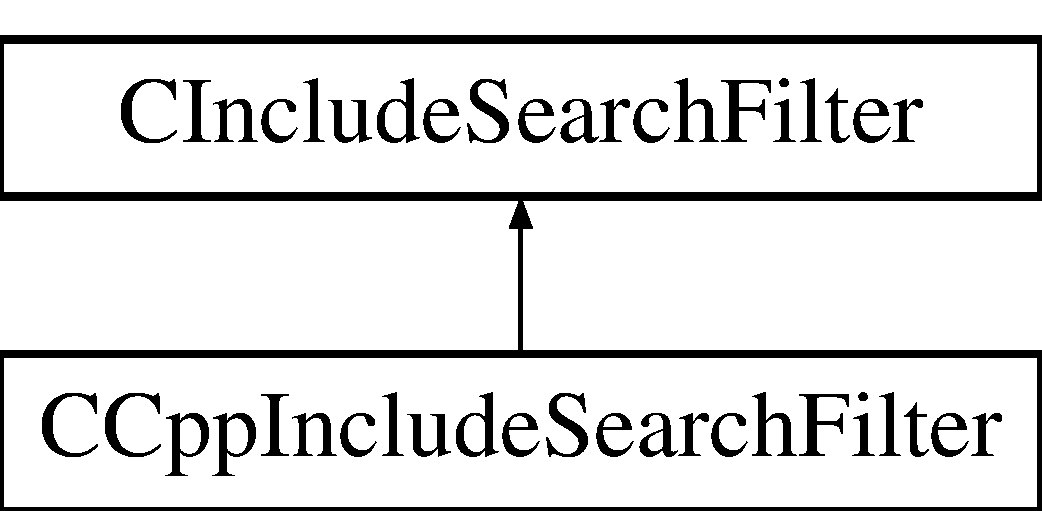
\includegraphics[height=2.000000cm]{d3/d80/classCCppIncludeSearchFilter}
\end{center}
\end{figure}
\subsection*{Public Member Functions}
\begin{DoxyCompactItemize}
\item 
virtual void \hyperlink{classCCppIncludeSearchFilter_a841ef5c22cdb587cc00e698312012944}{Assign} (const \hyperlink{classCCppIncludeSearchFilter}{C\-Cpp\-Include\-Search\-Filter} \&Filter)
\begin{DoxyCompactList}\small\item\em Copies filter settings from another filter. \end{DoxyCompactList}\item 
virtual bool \hyperlink{classCCppIncludeSearchFilter_a847f213a3ab4d7220a1ee0a095a5f42f}{Execute} (const \hyperlink{classCString}{C\-String} \&File\-Name, \hyperlink{classCStringList}{C\-String\-List} \&Includes)
\begin{DoxyCompactList}\small\item\em Gathers dependencies to {\itshape Includes} string list starting from {\itshape File\-Name} file. \end{DoxyCompactList}\item 
virtual bool \hyperlink{classCCppIncludeSearchFilter_ac37bc3584c554db6a7964c8e9de31636}{Execute} (const \hyperlink{classCString}{C\-String} \&File\-Name, \hyperlink{classCDependencyInfo}{C\-Dependency\-Info} \&Dependencies)
\begin{DoxyCompactList}\small\item\em Gathers dependencies to {\itshape Dependencies} database starting from {\itshape File\-Name} file. \end{DoxyCompactList}\item 
\hyperlink{classCCppIncludeSearchFilter_afc83d326ec4699a54887bad165609690}{C\-Cpp\-Include\-Search\-Filter} (void)
\begin{DoxyCompactList}\small\item\em Creates dependency search filter. \end{DoxyCompactList}\item 
\hyperlink{classCCppIncludeSearchFilter_a978515421bf849a4169e52e8977cdcfb}{C\-Cpp\-Include\-Search\-Filter} (const \hyperlink{classCCppIncludeSearchFilter}{C\-Cpp\-Include\-Search\-Filter} \&Filter)
\begin{DoxyCompactList}\small\item\em Copies dependency search filter from another filter. \end{DoxyCompactList}\item 
\hyperlink{classCCppIncludeSearchFilter_a64b222a54f46b366998decad4a953451}{$\sim$\-C\-Cpp\-Include\-Search\-Filter} (void)
\begin{DoxyCompactList}\small\item\em Destroys dependency search filter. \end{DoxyCompactList}\end{DoxyCompactItemize}
\subsection*{Additional Inherited Members}


\subsection{Detailed Description}
Gathers build unit dependencies from C/\-C++ source files withing project into build unit dependency database. 

\subsection{Constructor \& Destructor Documentation}
\hypertarget{classCCppIncludeSearchFilter_afc83d326ec4699a54887bad165609690}{\index{C\-Cpp\-Include\-Search\-Filter@{C\-Cpp\-Include\-Search\-Filter}!C\-Cpp\-Include\-Search\-Filter@{C\-Cpp\-Include\-Search\-Filter}}
\index{C\-Cpp\-Include\-Search\-Filter@{C\-Cpp\-Include\-Search\-Filter}!CCppIncludeSearchFilter@{C\-Cpp\-Include\-Search\-Filter}}
\subsubsection[{C\-Cpp\-Include\-Search\-Filter}]{\setlength{\rightskip}{0pt plus 5cm}C\-Cpp\-Include\-Search\-Filter\-::\-C\-Cpp\-Include\-Search\-Filter (
\begin{DoxyParamCaption}
\item[{void}]{}
\end{DoxyParamCaption}
)}}\label{classCCppIncludeSearchFilter_afc83d326ec4699a54887bad165609690}


Creates dependency search filter. 

\hypertarget{classCCppIncludeSearchFilter_a978515421bf849a4169e52e8977cdcfb}{\index{C\-Cpp\-Include\-Search\-Filter@{C\-Cpp\-Include\-Search\-Filter}!C\-Cpp\-Include\-Search\-Filter@{C\-Cpp\-Include\-Search\-Filter}}
\index{C\-Cpp\-Include\-Search\-Filter@{C\-Cpp\-Include\-Search\-Filter}!CCppIncludeSearchFilter@{C\-Cpp\-Include\-Search\-Filter}}
\subsubsection[{C\-Cpp\-Include\-Search\-Filter}]{\setlength{\rightskip}{0pt plus 5cm}C\-Cpp\-Include\-Search\-Filter\-::\-C\-Cpp\-Include\-Search\-Filter (
\begin{DoxyParamCaption}
\item[{const {\bf C\-Cpp\-Include\-Search\-Filter} \&}]{Filter}
\end{DoxyParamCaption}
)}}\label{classCCppIncludeSearchFilter_a978515421bf849a4169e52e8977cdcfb}


Copies dependency search filter from another filter. 


\begin{DoxyParams}{Parameters}
{\em Filter} & another dependency search filter. \\
\hline
\end{DoxyParams}
\hypertarget{classCCppIncludeSearchFilter_a64b222a54f46b366998decad4a953451}{\index{C\-Cpp\-Include\-Search\-Filter@{C\-Cpp\-Include\-Search\-Filter}!$\sim$\-C\-Cpp\-Include\-Search\-Filter@{$\sim$\-C\-Cpp\-Include\-Search\-Filter}}
\index{$\sim$\-C\-Cpp\-Include\-Search\-Filter@{$\sim$\-C\-Cpp\-Include\-Search\-Filter}!CCppIncludeSearchFilter@{C\-Cpp\-Include\-Search\-Filter}}
\subsubsection[{$\sim$\-C\-Cpp\-Include\-Search\-Filter}]{\setlength{\rightskip}{0pt plus 5cm}C\-Cpp\-Include\-Search\-Filter\-::$\sim$\-C\-Cpp\-Include\-Search\-Filter (
\begin{DoxyParamCaption}
\item[{void}]{}
\end{DoxyParamCaption}
)}}\label{classCCppIncludeSearchFilter_a64b222a54f46b366998decad4a953451}


Destroys dependency search filter. 



\subsection{Member Function Documentation}
\hypertarget{classCCppIncludeSearchFilter_a841ef5c22cdb587cc00e698312012944}{\index{C\-Cpp\-Include\-Search\-Filter@{C\-Cpp\-Include\-Search\-Filter}!Assign@{Assign}}
\index{Assign@{Assign}!CCppIncludeSearchFilter@{C\-Cpp\-Include\-Search\-Filter}}
\subsubsection[{Assign}]{\setlength{\rightskip}{0pt plus 5cm}C\-Cpp\-Include\-Search\-Filter\-::\-Assign (
\begin{DoxyParamCaption}
\item[{const {\bf C\-Cpp\-Include\-Search\-Filter} \&}]{Filter}
\end{DoxyParamCaption}
)\hspace{0.3cm}{\ttfamily [virtual]}}}\label{classCCppIncludeSearchFilter_a841ef5c22cdb587cc00e698312012944}


Copies filter settings from another filter. 


\begin{DoxyParams}{Parameters}
{\em Filter} & another filter. \\
\hline
\end{DoxyParams}
\hypertarget{classCCppIncludeSearchFilter_a847f213a3ab4d7220a1ee0a095a5f42f}{\index{C\-Cpp\-Include\-Search\-Filter@{C\-Cpp\-Include\-Search\-Filter}!Execute@{Execute}}
\index{Execute@{Execute}!CCppIncludeSearchFilter@{C\-Cpp\-Include\-Search\-Filter}}
\subsubsection[{Execute}]{\setlength{\rightskip}{0pt plus 5cm}bool C\-Cpp\-Include\-Search\-Filter\-::\-Execute (
\begin{DoxyParamCaption}
\item[{const {\bf C\-String} \&}]{File\-Name, }
\item[{{\bf C\-String\-List} \&}]{Includes}
\end{DoxyParamCaption}
)\hspace{0.3cm}{\ttfamily [virtual]}}}\label{classCCppIncludeSearchFilter_a847f213a3ab4d7220a1ee0a095a5f42f}


Gathers dependencies to {\itshape Includes} string list starting from {\itshape File\-Name} file. 

\begin{DoxyRefDesc}{Deprecated}
\item[\hyperlink{deprecated__deprecated000001}{Deprecated}]Use \hyperlink{classCIncludeSearchFilter_aa43b2d4b8f62c9d695490d5cd072c3bc}{C\-Include\-Search\-Filter\-::\-Execute(const C\-String\& File\-Name, C\-Dependency\-Info\& Dependencies)}.\end{DoxyRefDesc}

\begin{DoxyParams}{Parameters}
{\em File\-Name} & a build unit name. \\
\hline
{\em Includes} & a list of build unit names. \\
\hline
\end{DoxyParams}
\begin{DoxyReturn}{Returns}
{\itshape true} if dependencies were gather from at least one (starting) file, {\itshape false} otherwise. 
\end{DoxyReturn}


Reimplemented from \hyperlink{classCIncludeSearchFilter_a2b30667171e75cd5721e97b54eeb9182}{C\-Include\-Search\-Filter}.

\hypertarget{classCCppIncludeSearchFilter_ac37bc3584c554db6a7964c8e9de31636}{\index{C\-Cpp\-Include\-Search\-Filter@{C\-Cpp\-Include\-Search\-Filter}!Execute@{Execute}}
\index{Execute@{Execute}!CCppIncludeSearchFilter@{C\-Cpp\-Include\-Search\-Filter}}
\subsubsection[{Execute}]{\setlength{\rightskip}{0pt plus 5cm}bool C\-Cpp\-Include\-Search\-Filter\-::\-Execute (
\begin{DoxyParamCaption}
\item[{const {\bf C\-String} \&}]{File\-Name, }
\item[{{\bf C\-Dependency\-Info} \&}]{Dependencies}
\end{DoxyParamCaption}
)\hspace{0.3cm}{\ttfamily [virtual]}}}\label{classCCppIncludeSearchFilter_ac37bc3584c554db6a7964c8e9de31636}


Gathers dependencies to {\itshape Dependencies} database starting from {\itshape File\-Name} file. 


\begin{DoxyParams}{Parameters}
{\em File\-Name} & a build unit name. \\
\hline
{\em Dependencies} & a build unit dependency database. \\
\hline
\end{DoxyParams}
\begin{DoxyReturn}{Returns}
{\itshape true} if dependencies were gather from at least one (starting) file, {\itshape false} otherwise. 
\end{DoxyReturn}


Reimplemented from \hyperlink{classCIncludeSearchFilter_aa43b2d4b8f62c9d695490d5cd072c3bc}{C\-Include\-Search\-Filter}.



The documentation for this class was generated from the following files\-:\begin{DoxyCompactItemize}
\item 
src/\hyperlink{depsearch_8h}{depsearch.\-h}\item 
src/\hyperlink{depsearch_8cpp}{depsearch.\-cpp}\item 
src/doc/\hyperlink{depsearch_8dox}{depsearch.\-dox}\end{DoxyCompactItemize}

\hypertarget{classCDependencyGenerator}{\section{C\-Dependency\-Generator Class Reference}
\label{classCDependencyGenerator}\index{C\-Dependency\-Generator@{C\-Dependency\-Generator}}
}


{\ttfamily \#include $<$buildtools.\-h$>$}

Inheritance diagram for C\-Dependency\-Generator\-:\begin{figure}[H]
\begin{center}
\leavevmode
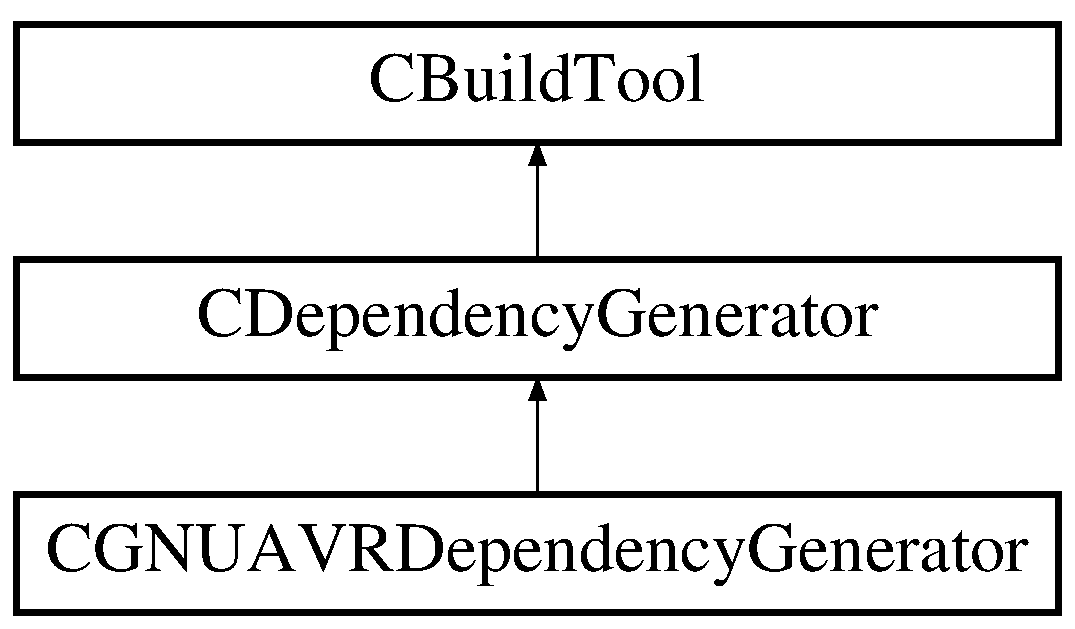
\includegraphics[height=3.000000cm]{dd/d5a/classCDependencyGenerator}
\end{center}
\end{figure}
\subsection*{Public Member Functions}
\begin{DoxyCompactItemize}
\item 
virtual \hyperlink{classCDependencyGenerator}{C\-Dependency\-Generator} $\ast$ \hyperlink{classCDependencyGenerator_af25a1710b95578b0e7ebcec02c4a7238}{Create\-Instance} (void)
\item 
virtual void \hyperlink{classCDependencyGenerator_aaaff3838bea1e65ba250b78f1746870c}{Read} (const Ti\-Xml\-Element $\ast$Build\-Tool\-Root)
\item 
virtual void \hyperlink{classCDependencyGenerator_a631a53bd18d1974f7375a665e17357a2}{Write} (Ti\-Xml\-Element $\ast$Build\-Tool\-Root)
\item 
virtual void \hyperlink{classCDependencyGenerator_a632c6eedf0b8d948748fb29f47545451}{Show} (void)
\item 
\hyperlink{classCDependencyGenerator_a286f57093ebd4b993c5a8e374abf74f9}{C\-Dependency\-Generator} (void)
\item 
\hyperlink{classCDependencyGenerator_aa79bde9f58c2051665f1c139e5661b94}{C\-Dependency\-Generator} (const \hyperlink{classCDependencyGenerator}{C\-Dependency\-Generator} \&Dependency\-Generator)
\item 
virtual \hyperlink{classCDependencyGenerator_a16c8c8474279be1dc68d76e0b5e34cb1}{$\sim$\-C\-Dependency\-Generator} (void)
\end{DoxyCompactItemize}
\subsection*{Additional Inherited Members}


\subsection{Constructor \& Destructor Documentation}
\hypertarget{classCDependencyGenerator_a286f57093ebd4b993c5a8e374abf74f9}{\index{C\-Dependency\-Generator@{C\-Dependency\-Generator}!C\-Dependency\-Generator@{C\-Dependency\-Generator}}
\index{C\-Dependency\-Generator@{C\-Dependency\-Generator}!CDependencyGenerator@{C\-Dependency\-Generator}}
\subsubsection[{C\-Dependency\-Generator}]{\setlength{\rightskip}{0pt plus 5cm}C\-Dependency\-Generator\-::\-C\-Dependency\-Generator (
\begin{DoxyParamCaption}
\item[{void}]{}
\end{DoxyParamCaption}
)}}\label{classCDependencyGenerator_a286f57093ebd4b993c5a8e374abf74f9}
\hypertarget{classCDependencyGenerator_aa79bde9f58c2051665f1c139e5661b94}{\index{C\-Dependency\-Generator@{C\-Dependency\-Generator}!C\-Dependency\-Generator@{C\-Dependency\-Generator}}
\index{C\-Dependency\-Generator@{C\-Dependency\-Generator}!CDependencyGenerator@{C\-Dependency\-Generator}}
\subsubsection[{C\-Dependency\-Generator}]{\setlength{\rightskip}{0pt plus 5cm}C\-Dependency\-Generator\-::\-C\-Dependency\-Generator (
\begin{DoxyParamCaption}
\item[{const {\bf C\-Dependency\-Generator} \&}]{Dependency\-Generator}
\end{DoxyParamCaption}
)}}\label{classCDependencyGenerator_aa79bde9f58c2051665f1c139e5661b94}
\hypertarget{classCDependencyGenerator_a16c8c8474279be1dc68d76e0b5e34cb1}{\index{C\-Dependency\-Generator@{C\-Dependency\-Generator}!$\sim$\-C\-Dependency\-Generator@{$\sim$\-C\-Dependency\-Generator}}
\index{$\sim$\-C\-Dependency\-Generator@{$\sim$\-C\-Dependency\-Generator}!CDependencyGenerator@{C\-Dependency\-Generator}}
\subsubsection[{$\sim$\-C\-Dependency\-Generator}]{\setlength{\rightskip}{0pt plus 5cm}C\-Dependency\-Generator\-::$\sim$\-C\-Dependency\-Generator (
\begin{DoxyParamCaption}
\item[{void}]{}
\end{DoxyParamCaption}
)\hspace{0.3cm}{\ttfamily [virtual]}}}\label{classCDependencyGenerator_a16c8c8474279be1dc68d76e0b5e34cb1}


\subsection{Member Function Documentation}
\hypertarget{classCDependencyGenerator_af25a1710b95578b0e7ebcec02c4a7238}{\index{C\-Dependency\-Generator@{C\-Dependency\-Generator}!Create\-Instance@{Create\-Instance}}
\index{Create\-Instance@{Create\-Instance}!CDependencyGenerator@{C\-Dependency\-Generator}}
\subsubsection[{Create\-Instance}]{\setlength{\rightskip}{0pt plus 5cm}{\bf C\-Dependency\-Generator} $\ast$ C\-Dependency\-Generator\-::\-Create\-Instance (
\begin{DoxyParamCaption}
\item[{void}]{}
\end{DoxyParamCaption}
)\hspace{0.3cm}{\ttfamily [virtual]}}}\label{classCDependencyGenerator_af25a1710b95578b0e7ebcec02c4a7238}


Reimplemented from \hyperlink{classCBuildTool_aa7f0e7c0bd7f75c71d37df066bcb581e}{C\-Build\-Tool}.



Reimplemented in \hyperlink{classCGNUAVRDependencyGenerator_a5d4d5e45d1cdd58d998ac961a66647dc}{C\-G\-N\-U\-A\-V\-R\-Dependency\-Generator}.

\hypertarget{classCDependencyGenerator_aaaff3838bea1e65ba250b78f1746870c}{\index{C\-Dependency\-Generator@{C\-Dependency\-Generator}!Read@{Read}}
\index{Read@{Read}!CDependencyGenerator@{C\-Dependency\-Generator}}
\subsubsection[{Read}]{\setlength{\rightskip}{0pt plus 5cm}void C\-Dependency\-Generator\-::\-Read (
\begin{DoxyParamCaption}
\item[{const Ti\-Xml\-Element $\ast$}]{Build\-Tool\-Root}
\end{DoxyParamCaption}
)\hspace{0.3cm}{\ttfamily [virtual]}}}\label{classCDependencyGenerator_aaaff3838bea1e65ba250b78f1746870c}


Reimplemented from \hyperlink{classCBuildTool_a299d87943c0f68dde5316318cc0838f8}{C\-Build\-Tool}.

\hypertarget{classCDependencyGenerator_a632c6eedf0b8d948748fb29f47545451}{\index{C\-Dependency\-Generator@{C\-Dependency\-Generator}!Show@{Show}}
\index{Show@{Show}!CDependencyGenerator@{C\-Dependency\-Generator}}
\subsubsection[{Show}]{\setlength{\rightskip}{0pt plus 5cm}void C\-Dependency\-Generator\-::\-Show (
\begin{DoxyParamCaption}
\item[{void}]{}
\end{DoxyParamCaption}
)\hspace{0.3cm}{\ttfamily [virtual]}}}\label{classCDependencyGenerator_a632c6eedf0b8d948748fb29f47545451}


Reimplemented from \hyperlink{classCBuildTool_a69815d1393a61dc16b2cc2d0552cd5ac}{C\-Build\-Tool}.

\hypertarget{classCDependencyGenerator_a631a53bd18d1974f7375a665e17357a2}{\index{C\-Dependency\-Generator@{C\-Dependency\-Generator}!Write@{Write}}
\index{Write@{Write}!CDependencyGenerator@{C\-Dependency\-Generator}}
\subsubsection[{Write}]{\setlength{\rightskip}{0pt plus 5cm}void C\-Dependency\-Generator\-::\-Write (
\begin{DoxyParamCaption}
\item[{Ti\-Xml\-Element $\ast$}]{Build\-Tool\-Root}
\end{DoxyParamCaption}
)\hspace{0.3cm}{\ttfamily [virtual]}}}\label{classCDependencyGenerator_a631a53bd18d1974f7375a665e17357a2}


Reimplemented from \hyperlink{classCBuildTool_af0331a777785bc2d15236b5c74321ed2}{C\-Build\-Tool}.



The documentation for this class was generated from the following files\-:\begin{DoxyCompactItemize}
\item 
src/\hyperlink{buildtools_8h}{buildtools.\-h}\item 
src/\hyperlink{buildtools_8cpp}{buildtools.\-cpp}\end{DoxyCompactItemize}

\hypertarget{classCDependencyInfo}{\section{C\-Dependency\-Info Class Reference}
\label{classCDependencyInfo}\index{C\-Dependency\-Info@{C\-Dependency\-Info}}
}


Dependency information for build units in a project.  




{\ttfamily \#include $<$depsearch.\-h$>$}

\subsection*{Public Member Functions}
\begin{DoxyCompactItemize}
\item 
\hyperlink{classCPlatform}{C\-Platform} \& \hyperlink{classCDependencyInfo_ae94f6374ec681801cc8304ad3e8a4f5e}{Platform} (void)
\begin{DoxyCompactList}\small\item\em Platform/\-O\-S type, generally used for creating compatible file paths. \end{DoxyCompactList}\item 
void \hyperlink{classCDependencyInfo_a900762f097ed041faa74613da4ea62c2}{Clear} (void)
\begin{DoxyCompactList}\small\item\em Resets the unit dependency database to the initial state. \end{DoxyCompactList}\item 
void \hyperlink{classCDependencyInfo_a946c31a0b7bef21a5793e6b134978912}{Show} (void)
\begin{DoxyCompactList}\small\item\em Print dependency information for all of build units to the standard output. \end{DoxyCompactList}\item 
\hyperlink{classCString}{C\-String} \hyperlink{classCDependencyInfo_ac2e36edc053c52d6fa9da19ef293e24b}{One\-Line\-Report} (const size\-\_\-t Index, const bool Deps, const bool X\-Refs)
\begin{DoxyCompactList}\small\item\em Returns a short string representation of dependency information. \end{DoxyCompactList}\item 
size\-\_\-t \hyperlink{classCDependencyInfo_a844740f473781d070df0f41d0762eb2f}{Records\-Count} (void) const 
\begin{DoxyCompactList}\small\item\em Returns the number of dependency records. \end{DoxyCompactList}\item 
\hyperlink{classCString}{C\-String} \hyperlink{classCDependencyInfo_abd5a916dfc975667d25d9216d15a3ccf}{Name} (const size\-\_\-t Index) const 
\begin{DoxyCompactList}\small\item\em Returns name of a build unit with dependency record number {\itshape Index}. \end{DoxyCompactList}\item 
size\-\_\-t \hyperlink{classCDependencyInfo_a22150f25fecc523402af14ea5c57d104}{Direct\-Dependencies\-Count} (const size\-\_\-t Index) const 
\begin{DoxyCompactList}\small\item\em Counts direct dependencies of a build unit with dependency record number {\itshape Index}. \end{DoxyCompactList}\item 
size\-\_\-t \hyperlink{classCDependencyInfo_a918389de5c0c99a3e69026ea0176c89e}{Indirect\-Dependencies\-Count} (const size\-\_\-t Index)
\begin{DoxyCompactList}\small\item\em Counts only indirect dependencies of a build unit with number {\itshape Index}. \end{DoxyCompactList}\item 
size\-\_\-t \hyperlink{classCDependencyInfo_acd47e7cf24369dd634b509c6932f7dca}{All\-Dependencies\-Count} (const size\-\_\-t Index)
\begin{DoxyCompactList}\small\item\em Returns the total count of dependencies of a build unit with dependency record number {\itshape Index}. \end{DoxyCompactList}\item 
\hyperlink{classCStringList}{C\-String\-List} \hyperlink{classCDependencyInfo_a00b6287cc4a978f8abfa2b1442175d24}{Direct\-Dependencies} (const size\-\_\-t Index) const 
\begin{DoxyCompactList}\small\item\em Returns a list of build unit names that a build unit with dependency record number {\itshape Index} depends on directly. \end{DoxyCompactList}\item 
\hyperlink{classCStringList}{C\-String\-List} \hyperlink{classCDependencyInfo_a51e609331ebc077d6eea5778fd8f8c8b}{Indirect\-Dependencies} (const size\-\_\-t Index)
\begin{DoxyCompactList}\small\item\em Returns a list of build unit names that a build unit with dependency record number {\itshape Index} depends on indirectly. \end{DoxyCompactList}\item 
\hyperlink{classCStringList}{C\-String\-List} \hyperlink{classCDependencyInfo_a02419d86ae1e14504c8657fb2d62bb4c}{All\-Dependencies} (const size\-\_\-t Index)
\begin{DoxyCompactList}\small\item\em Returns a complete list of build unit names that a build unit with dependency record number {\itshape Index} depends on directly or indirectly. \end{DoxyCompactList}\item 
size\-\_\-t \hyperlink{classCDependencyInfo_a4aa7031586c8dd2cc8dfa8ebc54dd9b2}{Direct\-Cross\-References\-Count} (const size\-\_\-t Index) const 
\begin{DoxyCompactList}\small\item\em Counts direct cross references to a build unit with dependency record number {\itshape Index}. \end{DoxyCompactList}\item 
size\-\_\-t \hyperlink{classCDependencyInfo_a3a4c4419cf30712a16bb71b2f9c7a87c}{Indirect\-Cross\-References\-Count} (const size\-\_\-t Index)
\begin{DoxyCompactList}\small\item\em Counts indirect cross references to a build unit with dependency record number {\itshape Index}. \end{DoxyCompactList}\item 
size\-\_\-t \hyperlink{classCDependencyInfo_aaf613223ecfb1d5decf8b38cb067ae25}{All\-Cross\-References\-Count} (const size\-\_\-t Index)
\begin{DoxyCompactList}\small\item\em Returns the total count of cross references of a build unit with dependency record number {\itshape Index}. \end{DoxyCompactList}\item 
\hyperlink{classCStringList}{C\-String\-List} \hyperlink{classCDependencyInfo_ac1182a8d99046fc6f735576d6b55fc73}{Direct\-Cross\-References} (const size\-\_\-t Index) const 
\begin{DoxyCompactList}\small\item\em Returns a list of build unit names that directly depend on a build unit with dependency record number {\itshape Index}. \end{DoxyCompactList}\item 
\hyperlink{classCStringList}{C\-String\-List} \hyperlink{classCDependencyInfo_aa2a9f2ea3bc0e5f3b71603a477fc5619}{Indirect\-Cross\-References} (const size\-\_\-t Index)
\begin{DoxyCompactList}\small\item\em Returns a list of build unit names that indirectly depend on a build unit with dependency record number {\itshape Index}. \end{DoxyCompactList}\item 
\hyperlink{classCStringList}{C\-String\-List} \hyperlink{classCDependencyInfo_ab07c351a53409894d86e9e10f7a70f7f}{All\-Cross\-References} (const size\-\_\-t Index)
\begin{DoxyCompactList}\small\item\em Returns a complete list of build unit names that depend on a build unit with dependency record number {\itshape Index} either directly or indirectly. \end{DoxyCompactList}\item 
bool \hyperlink{classCDependencyInfo_a3325672b42de84d6043fe47c666350a0}{Are\-Dependencies\-Complete} (const size\-\_\-t Index)
\begin{DoxyCompactList}\small\item\em Verifies if a dependency list for a build unit with dependency record number {\itshape Index} is marked as complete. \end{DoxyCompactList}\item 
bool \hyperlink{classCDependencyInfo_ae1ffc10e98443e562d6b8a8d7b1a869f}{Are\-Cross\-References\-Complete} (const size\-\_\-t Index)
\begin{DoxyCompactList}\small\item\em Verifies if a cross reference list for a build unit with dependency record number {\itshape Index} is marked as complete. \end{DoxyCompactList}\item 
void \hyperlink{classCDependencyInfo_aab60680f8f1c33981e9abe0ba132d744}{Set\-Dependencies\-Complete} (const size\-\_\-t Index, const bool State=true)
\begin{DoxyCompactList}\small\item\em Marks a dependency list for a build unit with dependency record number {\itshape Index} as complete. \end{DoxyCompactList}\item 
void \hyperlink{classCDependencyInfo_a433798f74d8db352e22dd5e4fd1268af}{Set\-Cross\-References\-Complete} (const size\-\_\-t Index, const bool State=true)
\begin{DoxyCompactList}\small\item\em Marks a cross reference list for a build unit with number {\itshape Index} as complete. \end{DoxyCompactList}\item 
int \hyperlink{classCDependencyInfo_ab3c71dc1906f859133771b4228b61c8e}{Find\-Record} (const \hyperlink{classCString}{C\-String} \&\hyperlink{classCDependencyInfo_abd5a916dfc975667d25d9216d15a3ccf}{Name})
\begin{DoxyCompactList}\small\item\em Performs dependency record lookup by a build unit name. \end{DoxyCompactList}\item 
size\-\_\-t \hyperlink{classCDependencyInfo_aae74e0642e410f1f2364908a6030f410}{Add\-Record} (const \hyperlink{classCString}{C\-String} \&\hyperlink{classCDependencyInfo_abd5a916dfc975667d25d9216d15a3ccf}{Name})
\begin{DoxyCompactList}\small\item\em Adds a new dependency record for the {\itshape Name} build unit. \end{DoxyCompactList}\item 
bool \hyperlink{classCDependencyInfo_aeee41f5696f9e0952d0bb8cef3adf311}{Add\-Dependency} (const size\-\_\-t Index, const \hyperlink{classCString}{C\-String} \&Dependency\-Name)
\begin{DoxyCompactList}\small\item\em Adds the {\itshape Dependency\-Name} build unit to a dependency record with number {\itshape Index}. \end{DoxyCompactList}\item 
size\-\_\-t \hyperlink{classCDependencyInfo_a927accf24328efc443082b1cf967a01a}{Add\-Dependency} (const \hyperlink{classCString}{C\-String} \&\hyperlink{classCDependencyInfo_abd5a916dfc975667d25d9216d15a3ccf}{Name}, const \hyperlink{classCString}{C\-String} \&Dependency\-Name)
\begin{DoxyCompactList}\small\item\em Adds the {\itshape Dependency\-Name} build unit to a dependency record of the {\itshape Name} build unit. \end{DoxyCompactList}\item 
void \hyperlink{classCDependencyInfo_a076227951bd7f5e01db97e6e40eb5955}{Make\-Rules} (\hyperlink{classCMakefile}{C\-Makefile} \&Makefile, const int Section, const bool Multiline)
\begin{DoxyCompactList}\small\item\em Generates makefile rules for build unit dependencies. \end{DoxyCompactList}\item 
\hyperlink{classCDependencyInfo_a4fff8f942c388852af5b1a3ebd235d70}{C\-Dependency\-Info} (void)
\begin{DoxyCompactList}\small\item\em Creates build unit dependency database. \end{DoxyCompactList}\item 
\hyperlink{classCDependencyInfo_a1674b17fa54f4e53571ce9aac6abd88e}{$\sim$\-C\-Dependency\-Info} (void)
\begin{DoxyCompactList}\small\item\em Destroys build unit dependency database. \end{DoxyCompactList}\end{DoxyCompactItemize}
\subsection*{Private Member Functions}
\begin{DoxyCompactItemize}
\item 
void \hyperlink{classCDependencyInfo_a437ff774f21c51a187ad9a0b7ffbfa93}{Reset\-Markers} (void)
\begin{DoxyCompactList}\small\item\em Clears \hyperlink{classCDependencyRecord_a0327e854ac8b0bc48eefe3155a84475e}{C\-Dependency\-Record\-::m\-\_\-\-Marker} for all records in \hyperlink{classCDependencyInfo_ad76c0932810b200455ce757da050cda2}{C\-Dependency\-Info\-::m\-\_\-\-Records}. \end{DoxyCompactList}\item 
size\-\_\-t \hyperlink{classCDependencyInfo_a3ce43638906ad7dcc21f4ea8664ab34e}{Dependencies\-Count} (\hyperlink{classCDependencyRecord}{C\-Dependency\-Record} $\ast$Record)
\begin{DoxyCompactList}\small\item\em Returns the number of dependencies for a build unit pointed by {\itshape Record}. \end{DoxyCompactList}\item 
\hyperlink{classCStringList}{C\-String\-List} \hyperlink{classCDependencyInfo_aebc22dfe747ed1208ab4a16a396e7afb}{Dependencies} (\hyperlink{classCDependencyRecord}{C\-Dependency\-Record} $\ast$Record)
\begin{DoxyCompactList}\small\item\em Returns the list of file names of build units that a build unit pointed by {\itshape Record} depends on. \end{DoxyCompactList}\item 
size\-\_\-t \hyperlink{classCDependencyInfo_a2f6a15907c7ccb90c9dc1466d565241f}{Cross\-References\-Count} (\hyperlink{classCDependencyRecord}{C\-Dependency\-Record} $\ast$Record)
\begin{DoxyCompactList}\small\item\em Returns the number of cross references for a build unit pointed by {\itshape Record}. \end{DoxyCompactList}\item 
\hyperlink{classCStringList}{C\-String\-List} \hyperlink{classCDependencyInfo_ab93f959d3c0430039430a73562080b90}{Cross\-References} (\hyperlink{classCDependencyRecord}{C\-Dependency\-Record} $\ast$Record)
\begin{DoxyCompactList}\small\item\em Returns the list of file names of build units that depend on a build unit pointed by {\itshape Record}. \end{DoxyCompactList}\end{DoxyCompactItemize}
\subsection*{Private Attributes}
\begin{DoxyCompactItemize}
\item 
\hyperlink{classCPlatform}{C\-Platform} \hyperlink{classCDependencyInfo_a6a7fb9ef5de03c0013ce3aa3774d469c}{m\-\_\-\-Platform}
\begin{DoxyCompactList}\small\item\em Platform/\-O\-S type, generally used for creating compatible file paths. \end{DoxyCompactList}\item 
std\-::vector$<$ \hyperlink{classCDependencyRecord}{C\-Dependency\-Record} $\ast$ $>$ \hyperlink{classCDependencyInfo_ad76c0932810b200455ce757da050cda2}{m\-\_\-\-Records}
\begin{DoxyCompactList}\small\item\em Database of build unit dependencies. \end{DoxyCompactList}\end{DoxyCompactItemize}


\subsection{Detailed Description}
Dependency information for build units in a project. 

Stores a database of build unit dependencies and cross references, searches and unwinds dependncies of a particular unit, writes makefile rules for unit dependencies. Generally speaking, \hyperlink{classCDependencyInfo}{C\-Dependency\-Info} tracks only dependencies between abstract names (strings), it doesn't really care whether those names are real file names or build units or not. The only exception to that is providing platform information to a dependency search filter like \hyperlink{classCIncludeSearchFilter}{C\-Include\-Search\-Filter} and its descendants for building compatible file paths. 

\subsection{Constructor \& Destructor Documentation}
\hypertarget{classCDependencyInfo_a4fff8f942c388852af5b1a3ebd235d70}{\index{C\-Dependency\-Info@{C\-Dependency\-Info}!C\-Dependency\-Info@{C\-Dependency\-Info}}
\index{C\-Dependency\-Info@{C\-Dependency\-Info}!CDependencyInfo@{C\-Dependency\-Info}}
\subsubsection[{C\-Dependency\-Info}]{\setlength{\rightskip}{0pt plus 5cm}C\-Dependency\-Info\-::\-C\-Dependency\-Info (
\begin{DoxyParamCaption}
\item[{void}]{}
\end{DoxyParamCaption}
)}}\label{classCDependencyInfo_a4fff8f942c388852af5b1a3ebd235d70}


Creates build unit dependency database. 

\hypertarget{classCDependencyInfo_a1674b17fa54f4e53571ce9aac6abd88e}{\index{C\-Dependency\-Info@{C\-Dependency\-Info}!$\sim$\-C\-Dependency\-Info@{$\sim$\-C\-Dependency\-Info}}
\index{$\sim$\-C\-Dependency\-Info@{$\sim$\-C\-Dependency\-Info}!CDependencyInfo@{C\-Dependency\-Info}}
\subsubsection[{$\sim$\-C\-Dependency\-Info}]{\setlength{\rightskip}{0pt plus 5cm}C\-Dependency\-Info\-::$\sim$\-C\-Dependency\-Info (
\begin{DoxyParamCaption}
\item[{void}]{}
\end{DoxyParamCaption}
)}}\label{classCDependencyInfo_a1674b17fa54f4e53571ce9aac6abd88e}


Destroys build unit dependency database. 



\subsection{Member Function Documentation}
\hypertarget{classCDependencyInfo_aeee41f5696f9e0952d0bb8cef3adf311}{\index{C\-Dependency\-Info@{C\-Dependency\-Info}!Add\-Dependency@{Add\-Dependency}}
\index{Add\-Dependency@{Add\-Dependency}!CDependencyInfo@{C\-Dependency\-Info}}
\subsubsection[{Add\-Dependency}]{\setlength{\rightskip}{0pt plus 5cm}C\-Dependency\-Info\-::\-Add\-Dependency (
\begin{DoxyParamCaption}
\item[{const size\-\_\-t}]{Index, }
\item[{const {\bf C\-String} \&}]{Dependency\-Name}
\end{DoxyParamCaption}
)}}\label{classCDependencyInfo_aeee41f5696f9e0952d0bb8cef3adf311}


Adds the {\itshape Dependency\-Name} build unit to a dependency record with number {\itshape Index}. 


\begin{DoxyParams}{Parameters}
{\em Index} & number of a dependency record of a build unit. \\
\hline
{\em Dependency\-Name} & name of another build unit. \\
\hline
\end{DoxyParams}
\begin{DoxyReturn}{Returns}
true, if {\itshape Index} is a valid number of a dependency record, {\itshape false} otherwise. 
\end{DoxyReturn}
\hypertarget{classCDependencyInfo_a927accf24328efc443082b1cf967a01a}{\index{C\-Dependency\-Info@{C\-Dependency\-Info}!Add\-Dependency@{Add\-Dependency}}
\index{Add\-Dependency@{Add\-Dependency}!CDependencyInfo@{C\-Dependency\-Info}}
\subsubsection[{Add\-Dependency}]{\setlength{\rightskip}{0pt plus 5cm}C\-Dependency\-Info\-::\-Add\-Dependency (
\begin{DoxyParamCaption}
\item[{const {\bf C\-String} \&}]{Name, }
\item[{const {\bf C\-String} \&}]{Dependency\-Name}
\end{DoxyParamCaption}
)}}\label{classCDependencyInfo_a927accf24328efc443082b1cf967a01a}


Adds the {\itshape Dependency\-Name} build unit to a dependency record of the {\itshape Name} build unit. 


\begin{DoxyParams}{Parameters}
{\em Name} & name of a build unit. \\
\hline
{\em Dependency\-Name} & name of another build unit. \\
\hline
\end{DoxyParams}
\begin{DoxyReturn}{Returns}
number of a dependency record of the {\itshape Name} build unit. 
\end{DoxyReturn}
\hypertarget{classCDependencyInfo_aae74e0642e410f1f2364908a6030f410}{\index{C\-Dependency\-Info@{C\-Dependency\-Info}!Add\-Record@{Add\-Record}}
\index{Add\-Record@{Add\-Record}!CDependencyInfo@{C\-Dependency\-Info}}
\subsubsection[{Add\-Record}]{\setlength{\rightskip}{0pt plus 5cm}C\-Dependency\-Info\-::\-Add\-Record (
\begin{DoxyParamCaption}
\item[{const {\bf C\-String} \&}]{Name}
\end{DoxyParamCaption}
)}}\label{classCDependencyInfo_aae74e0642e410f1f2364908a6030f410}


Adds a new dependency record for the {\itshape Name} build unit. 


\begin{DoxyParams}{Parameters}
{\em Name} & name of a build unit. \\
\hline
\end{DoxyParams}
\begin{DoxyReturn}{Returns}
number (index) of the new dependency record. 
\end{DoxyReturn}
\hypertarget{classCDependencyInfo_ab07c351a53409894d86e9e10f7a70f7f}{\index{C\-Dependency\-Info@{C\-Dependency\-Info}!All\-Cross\-References@{All\-Cross\-References}}
\index{All\-Cross\-References@{All\-Cross\-References}!CDependencyInfo@{C\-Dependency\-Info}}
\subsubsection[{All\-Cross\-References}]{\setlength{\rightskip}{0pt plus 5cm}C\-Dependency\-Info\-::\-All\-Cross\-References (
\begin{DoxyParamCaption}
\item[{const size\-\_\-t}]{Index}
\end{DoxyParamCaption}
)}}\label{classCDependencyInfo_ab07c351a53409894d86e9e10f7a70f7f}


Returns a complete list of build unit names that depend on a build unit with dependency record number {\itshape Index} either directly or indirectly. 


\begin{DoxyParams}{Parameters}
{\em Index} & number of a dependency record. \\
\hline
\end{DoxyParams}
\begin{DoxyReturn}{Returns}
list of build unit names. 
\end{DoxyReturn}
\hypertarget{classCDependencyInfo_aaf613223ecfb1d5decf8b38cb067ae25}{\index{C\-Dependency\-Info@{C\-Dependency\-Info}!All\-Cross\-References\-Count@{All\-Cross\-References\-Count}}
\index{All\-Cross\-References\-Count@{All\-Cross\-References\-Count}!CDependencyInfo@{C\-Dependency\-Info}}
\subsubsection[{All\-Cross\-References\-Count}]{\setlength{\rightskip}{0pt plus 5cm}C\-Dependency\-Info\-::\-All\-Cross\-References\-Count (
\begin{DoxyParamCaption}
\item[{const size\-\_\-t}]{Index}
\end{DoxyParamCaption}
)}}\label{classCDependencyInfo_aaf613223ecfb1d5decf8b38cb067ae25}


Returns the total count of cross references of a build unit with dependency record number {\itshape Index}. 


\begin{DoxyParams}{Parameters}
{\em Index} & number of a dependency record. \\
\hline
\end{DoxyParams}
\begin{DoxyReturn}{Returns}
cross references count. 
\end{DoxyReturn}
\hypertarget{classCDependencyInfo_a02419d86ae1e14504c8657fb2d62bb4c}{\index{C\-Dependency\-Info@{C\-Dependency\-Info}!All\-Dependencies@{All\-Dependencies}}
\index{All\-Dependencies@{All\-Dependencies}!CDependencyInfo@{C\-Dependency\-Info}}
\subsubsection[{All\-Dependencies}]{\setlength{\rightskip}{0pt plus 5cm}C\-Dependency\-Info\-::\-All\-Dependencies (
\begin{DoxyParamCaption}
\item[{const size\-\_\-t}]{Index}
\end{DoxyParamCaption}
)}}\label{classCDependencyInfo_a02419d86ae1e14504c8657fb2d62bb4c}


Returns a complete list of build unit names that a build unit with dependency record number {\itshape Index} depends on directly or indirectly. 


\begin{DoxyParams}{Parameters}
{\em Index} & number of a dependency record. \\
\hline
\end{DoxyParams}
\begin{DoxyReturn}{Returns}
list of build unit names. 
\end{DoxyReturn}
\hypertarget{classCDependencyInfo_acd47e7cf24369dd634b509c6932f7dca}{\index{C\-Dependency\-Info@{C\-Dependency\-Info}!All\-Dependencies\-Count@{All\-Dependencies\-Count}}
\index{All\-Dependencies\-Count@{All\-Dependencies\-Count}!CDependencyInfo@{C\-Dependency\-Info}}
\subsubsection[{All\-Dependencies\-Count}]{\setlength{\rightskip}{0pt plus 5cm}C\-Dependency\-Info\-::\-All\-Dependencies\-Count (
\begin{DoxyParamCaption}
\item[{const size\-\_\-t}]{Index}
\end{DoxyParamCaption}
)}}\label{classCDependencyInfo_acd47e7cf24369dd634b509c6932f7dca}


Returns the total count of dependencies of a build unit with dependency record number {\itshape Index}. 


\begin{DoxyParams}{Parameters}
{\em Index} & number of a dependency record. \\
\hline
\end{DoxyParams}
\begin{DoxyReturn}{Returns}
sum of direct and indirect dependencies. 
\end{DoxyReturn}
\hypertarget{classCDependencyInfo_ae1ffc10e98443e562d6b8a8d7b1a869f}{\index{C\-Dependency\-Info@{C\-Dependency\-Info}!Are\-Cross\-References\-Complete@{Are\-Cross\-References\-Complete}}
\index{Are\-Cross\-References\-Complete@{Are\-Cross\-References\-Complete}!CDependencyInfo@{C\-Dependency\-Info}}
\subsubsection[{Are\-Cross\-References\-Complete}]{\setlength{\rightskip}{0pt plus 5cm}C\-Dependency\-Info\-::\-Are\-Cross\-References\-Complete (
\begin{DoxyParamCaption}
\item[{const size\-\_\-t}]{Index}
\end{DoxyParamCaption}
)}}\label{classCDependencyInfo_ae1ffc10e98443e562d6b8a8d7b1a869f}


Verifies if a cross reference list for a build unit with dependency record number {\itshape Index} is marked as complete. 


\begin{DoxyParams}{Parameters}
{\em Index} & number of a dependency record. \\
\hline
\end{DoxyParams}
\begin{DoxyReturn}{Returns}
{\itshape true} if a cross rference list is complete, {\itshape false} otherwise. 
\end{DoxyReturn}
\hypertarget{classCDependencyInfo_a3325672b42de84d6043fe47c666350a0}{\index{C\-Dependency\-Info@{C\-Dependency\-Info}!Are\-Dependencies\-Complete@{Are\-Dependencies\-Complete}}
\index{Are\-Dependencies\-Complete@{Are\-Dependencies\-Complete}!CDependencyInfo@{C\-Dependency\-Info}}
\subsubsection[{Are\-Dependencies\-Complete}]{\setlength{\rightskip}{0pt plus 5cm}C\-Dependency\-Info\-::\-Are\-Dependencies\-Complete (
\begin{DoxyParamCaption}
\item[{const size\-\_\-t}]{Index}
\end{DoxyParamCaption}
)}}\label{classCDependencyInfo_a3325672b42de84d6043fe47c666350a0}


Verifies if a dependency list for a build unit with dependency record number {\itshape Index} is marked as complete. 


\begin{DoxyParams}{Parameters}
{\em Index} & number of a dependency record. \\
\hline
\end{DoxyParams}
\begin{DoxyReturn}{Returns}
{\itshape true} if a dependency list is complete, {\itshape false} otherwise. 
\end{DoxyReturn}
\hypertarget{classCDependencyInfo_a900762f097ed041faa74613da4ea62c2}{\index{C\-Dependency\-Info@{C\-Dependency\-Info}!Clear@{Clear}}
\index{Clear@{Clear}!CDependencyInfo@{C\-Dependency\-Info}}
\subsubsection[{Clear}]{\setlength{\rightskip}{0pt plus 5cm}C\-Dependency\-Info\-::\-Clear (
\begin{DoxyParamCaption}
\item[{void}]{}
\end{DoxyParamCaption}
)}}\label{classCDependencyInfo_a900762f097ed041faa74613da4ea62c2}


Resets the unit dependency database to the initial state. 

\hypertarget{classCDependencyInfo_ab93f959d3c0430039430a73562080b90}{\index{C\-Dependency\-Info@{C\-Dependency\-Info}!Cross\-References@{Cross\-References}}
\index{Cross\-References@{Cross\-References}!CDependencyInfo@{C\-Dependency\-Info}}
\subsubsection[{Cross\-References}]{\setlength{\rightskip}{0pt plus 5cm}C\-Dependency\-Info\-::\-Cross\-References (
\begin{DoxyParamCaption}
\item[{{\bf C\-Dependency\-Record} $\ast$}]{Record}
\end{DoxyParamCaption}
)\hspace{0.3cm}{\ttfamily [private]}}}\label{classCDependencyInfo_ab93f959d3c0430039430a73562080b90}


Returns the list of file names of build units that depend on a build unit pointed by {\itshape Record}. 


\begin{DoxyParams}{Parameters}
{\em Record} & dependency record of a build unit.\\
\hline
\end{DoxyParams}
\begin{DoxyReturn}{Returns}
list of file names. 
\end{DoxyReturn}
\hypertarget{classCDependencyInfo_a2f6a15907c7ccb90c9dc1466d565241f}{\index{C\-Dependency\-Info@{C\-Dependency\-Info}!Cross\-References\-Count@{Cross\-References\-Count}}
\index{Cross\-References\-Count@{Cross\-References\-Count}!CDependencyInfo@{C\-Dependency\-Info}}
\subsubsection[{Cross\-References\-Count}]{\setlength{\rightskip}{0pt plus 5cm}C\-Dependency\-Info\-::\-Cross\-References\-Count (
\begin{DoxyParamCaption}
\item[{{\bf C\-Dependency\-Record} $\ast$}]{Record}
\end{DoxyParamCaption}
)\hspace{0.3cm}{\ttfamily [private]}}}\label{classCDependencyInfo_a2f6a15907c7ccb90c9dc1466d565241f}


Returns the number of cross references for a build unit pointed by {\itshape Record}. 


\begin{DoxyParams}{Parameters}
{\em Record} & dependency record of a build unit.\\
\hline
\end{DoxyParams}
\begin{DoxyReturn}{Returns}
cross references count. 
\end{DoxyReturn}
\hypertarget{classCDependencyInfo_aebc22dfe747ed1208ab4a16a396e7afb}{\index{C\-Dependency\-Info@{C\-Dependency\-Info}!Dependencies@{Dependencies}}
\index{Dependencies@{Dependencies}!CDependencyInfo@{C\-Dependency\-Info}}
\subsubsection[{Dependencies}]{\setlength{\rightskip}{0pt plus 5cm}C\-Dependency\-Info\-::\-Dependencies (
\begin{DoxyParamCaption}
\item[{{\bf C\-Dependency\-Record} $\ast$}]{Record}
\end{DoxyParamCaption}
)\hspace{0.3cm}{\ttfamily [private]}}}\label{classCDependencyInfo_aebc22dfe747ed1208ab4a16a396e7afb}


Returns the list of file names of build units that a build unit pointed by {\itshape Record} depends on. 


\begin{DoxyParams}{Parameters}
{\em Record} & dependency record of a build unit.\\
\hline
\end{DoxyParams}
\begin{DoxyReturn}{Returns}
list of file names. 
\end{DoxyReturn}
\hypertarget{classCDependencyInfo_a3ce43638906ad7dcc21f4ea8664ab34e}{\index{C\-Dependency\-Info@{C\-Dependency\-Info}!Dependencies\-Count@{Dependencies\-Count}}
\index{Dependencies\-Count@{Dependencies\-Count}!CDependencyInfo@{C\-Dependency\-Info}}
\subsubsection[{Dependencies\-Count}]{\setlength{\rightskip}{0pt plus 5cm}C\-Dependency\-Info\-::\-Dependencies\-Count (
\begin{DoxyParamCaption}
\item[{{\bf C\-Dependency\-Record} $\ast$}]{Record}
\end{DoxyParamCaption}
)\hspace{0.3cm}{\ttfamily [private]}}}\label{classCDependencyInfo_a3ce43638906ad7dcc21f4ea8664ab34e}


Returns the number of dependencies for a build unit pointed by {\itshape Record}. 


\begin{DoxyParams}{Parameters}
{\em Record} & dependency record of a build unit.\\
\hline
\end{DoxyParams}
\begin{DoxyReturn}{Returns}
dependencies count. 
\end{DoxyReturn}
\hypertarget{classCDependencyInfo_ac1182a8d99046fc6f735576d6b55fc73}{\index{C\-Dependency\-Info@{C\-Dependency\-Info}!Direct\-Cross\-References@{Direct\-Cross\-References}}
\index{Direct\-Cross\-References@{Direct\-Cross\-References}!CDependencyInfo@{C\-Dependency\-Info}}
\subsubsection[{Direct\-Cross\-References}]{\setlength{\rightskip}{0pt plus 5cm}C\-Dependency\-Info\-::\-Direct\-Cross\-References (
\begin{DoxyParamCaption}
\item[{const size\-\_\-t}]{Index}
\end{DoxyParamCaption}
) const}}\label{classCDependencyInfo_ac1182a8d99046fc6f735576d6b55fc73}


Returns a list of build unit names that directly depend on a build unit with dependency record number {\itshape Index}. 


\begin{DoxyParams}{Parameters}
{\em Index} & number of a dependency record. \\
\hline
\end{DoxyParams}
\begin{DoxyReturn}{Returns}
list of build unit names. 
\end{DoxyReturn}
\hypertarget{classCDependencyInfo_a4aa7031586c8dd2cc8dfa8ebc54dd9b2}{\index{C\-Dependency\-Info@{C\-Dependency\-Info}!Direct\-Cross\-References\-Count@{Direct\-Cross\-References\-Count}}
\index{Direct\-Cross\-References\-Count@{Direct\-Cross\-References\-Count}!CDependencyInfo@{C\-Dependency\-Info}}
\subsubsection[{Direct\-Cross\-References\-Count}]{\setlength{\rightskip}{0pt plus 5cm}C\-Dependency\-Info\-::\-Direct\-Cross\-References\-Count (
\begin{DoxyParamCaption}
\item[{const size\-\_\-t}]{Index}
\end{DoxyParamCaption}
) const}}\label{classCDependencyInfo_a4aa7031586c8dd2cc8dfa8ebc54dd9b2}


Counts direct cross references to a build unit with dependency record number {\itshape Index}. 


\begin{DoxyParams}{Parameters}
{\em Index} & number of a build unit. \\
\hline
\end{DoxyParams}
\begin{DoxyReturn}{Returns}
cross references count. 
\end{DoxyReturn}
\hypertarget{classCDependencyInfo_a00b6287cc4a978f8abfa2b1442175d24}{\index{C\-Dependency\-Info@{C\-Dependency\-Info}!Direct\-Dependencies@{Direct\-Dependencies}}
\index{Direct\-Dependencies@{Direct\-Dependencies}!CDependencyInfo@{C\-Dependency\-Info}}
\subsubsection[{Direct\-Dependencies}]{\setlength{\rightskip}{0pt plus 5cm}C\-Dependency\-Info\-::\-Direct\-Dependencies (
\begin{DoxyParamCaption}
\item[{const size\-\_\-t}]{Index}
\end{DoxyParamCaption}
) const}}\label{classCDependencyInfo_a00b6287cc4a978f8abfa2b1442175d24}


Returns a list of build unit names that a build unit with dependency record number {\itshape Index} depends on directly. 


\begin{DoxyParams}{Parameters}
{\em Index} & number of a dependency record. \\
\hline
\end{DoxyParams}
\begin{DoxyReturn}{Returns}
list of build unit names. 
\end{DoxyReturn}
\hypertarget{classCDependencyInfo_a22150f25fecc523402af14ea5c57d104}{\index{C\-Dependency\-Info@{C\-Dependency\-Info}!Direct\-Dependencies\-Count@{Direct\-Dependencies\-Count}}
\index{Direct\-Dependencies\-Count@{Direct\-Dependencies\-Count}!CDependencyInfo@{C\-Dependency\-Info}}
\subsubsection[{Direct\-Dependencies\-Count}]{\setlength{\rightskip}{0pt plus 5cm}C\-Dependency\-Info\-::\-Direct\-Dependencies\-Count (
\begin{DoxyParamCaption}
\item[{const size\-\_\-t}]{Index}
\end{DoxyParamCaption}
) const}}\label{classCDependencyInfo_a22150f25fecc523402af14ea5c57d104}


Counts direct dependencies of a build unit with dependency record number {\itshape Index}. 


\begin{DoxyParams}{Parameters}
{\em Index} & number of a dependency record.\\
\hline
\end{DoxyParams}
\begin{DoxyReturn}{Returns}
dependencies count. 
\end{DoxyReturn}
\hypertarget{classCDependencyInfo_ab3c71dc1906f859133771b4228b61c8e}{\index{C\-Dependency\-Info@{C\-Dependency\-Info}!Find\-Record@{Find\-Record}}
\index{Find\-Record@{Find\-Record}!CDependencyInfo@{C\-Dependency\-Info}}
\subsubsection[{Find\-Record}]{\setlength{\rightskip}{0pt plus 5cm}C\-Dependency\-Info\-::\-Find\-Record (
\begin{DoxyParamCaption}
\item[{const {\bf C\-String} \&}]{Name}
\end{DoxyParamCaption}
)}}\label{classCDependencyInfo_ab3c71dc1906f859133771b4228b61c8e}


Performs dependency record lookup by a build unit name. 


\begin{DoxyParams}{Parameters}
{\em Name} & name of a build unit. \\
\hline
\end{DoxyParams}
\begin{DoxyReturn}{Returns}
number (index) of the corresponding dependency record or -\/1 if no dependency record for the {\itshape Name} build unit is found. 
\end{DoxyReturn}
\hypertarget{classCDependencyInfo_aa2a9f2ea3bc0e5f3b71603a477fc5619}{\index{C\-Dependency\-Info@{C\-Dependency\-Info}!Indirect\-Cross\-References@{Indirect\-Cross\-References}}
\index{Indirect\-Cross\-References@{Indirect\-Cross\-References}!CDependencyInfo@{C\-Dependency\-Info}}
\subsubsection[{Indirect\-Cross\-References}]{\setlength{\rightskip}{0pt plus 5cm}C\-Dependency\-Info\-::\-Indirect\-Cross\-References (
\begin{DoxyParamCaption}
\item[{const size\-\_\-t}]{Index}
\end{DoxyParamCaption}
)}}\label{classCDependencyInfo_aa2a9f2ea3bc0e5f3b71603a477fc5619}


Returns a list of build unit names that indirectly depend on a build unit with dependency record number {\itshape Index}. 


\begin{DoxyParams}{Parameters}
{\em Index} & number of a dependency record. \\
\hline
\end{DoxyParams}
\begin{DoxyReturn}{Returns}
list of build unit names. 
\end{DoxyReturn}
\hypertarget{classCDependencyInfo_a3a4c4419cf30712a16bb71b2f9c7a87c}{\index{C\-Dependency\-Info@{C\-Dependency\-Info}!Indirect\-Cross\-References\-Count@{Indirect\-Cross\-References\-Count}}
\index{Indirect\-Cross\-References\-Count@{Indirect\-Cross\-References\-Count}!CDependencyInfo@{C\-Dependency\-Info}}
\subsubsection[{Indirect\-Cross\-References\-Count}]{\setlength{\rightskip}{0pt plus 5cm}C\-Dependency\-Info\-::\-Indirect\-Cross\-References\-Count (
\begin{DoxyParamCaption}
\item[{const size\-\_\-t}]{Index}
\end{DoxyParamCaption}
)}}\label{classCDependencyInfo_a3a4c4419cf30712a16bb71b2f9c7a87c}


Counts indirect cross references to a build unit with dependency record number {\itshape Index}. 


\begin{DoxyParams}{Parameters}
{\em Index} & number of a dependency record. \\
\hline
\end{DoxyParams}
\begin{DoxyReturn}{Returns}
cross references count. 
\end{DoxyReturn}
\hypertarget{classCDependencyInfo_a51e609331ebc077d6eea5778fd8f8c8b}{\index{C\-Dependency\-Info@{C\-Dependency\-Info}!Indirect\-Dependencies@{Indirect\-Dependencies}}
\index{Indirect\-Dependencies@{Indirect\-Dependencies}!CDependencyInfo@{C\-Dependency\-Info}}
\subsubsection[{Indirect\-Dependencies}]{\setlength{\rightskip}{0pt plus 5cm}C\-Dependency\-Info\-::\-Indirect\-Dependencies (
\begin{DoxyParamCaption}
\item[{const size\-\_\-t}]{Index}
\end{DoxyParamCaption}
)}}\label{classCDependencyInfo_a51e609331ebc077d6eea5778fd8f8c8b}


Returns a list of build unit names that a build unit with dependency record number {\itshape Index} depends on indirectly. 


\begin{DoxyParams}{Parameters}
{\em Index} & number of a dependency record. \\
\hline
\end{DoxyParams}
\begin{DoxyReturn}{Returns}
list of build unit names. 
\end{DoxyReturn}
\hypertarget{classCDependencyInfo_a918389de5c0c99a3e69026ea0176c89e}{\index{C\-Dependency\-Info@{C\-Dependency\-Info}!Indirect\-Dependencies\-Count@{Indirect\-Dependencies\-Count}}
\index{Indirect\-Dependencies\-Count@{Indirect\-Dependencies\-Count}!CDependencyInfo@{C\-Dependency\-Info}}
\subsubsection[{Indirect\-Dependencies\-Count}]{\setlength{\rightskip}{0pt plus 5cm}C\-Dependency\-Info\-::\-Indirect\-Dependencies\-Count (
\begin{DoxyParamCaption}
\item[{const size\-\_\-t}]{Index}
\end{DoxyParamCaption}
)}}\label{classCDependencyInfo_a918389de5c0c99a3e69026ea0176c89e}


Counts only indirect dependencies of a build unit with number {\itshape Index}. 


\begin{DoxyParams}{Parameters}
{\em Index} & number of a build unit. \\
\hline
\end{DoxyParams}
\begin{DoxyReturn}{Returns}
dependencies count.
\end{DoxyReturn}
Indirect dependencies are dependencies of all build units that selected build unit with number {\itshape Index} depends on excluding these units. \hypertarget{classCDependencyInfo_a076227951bd7f5e01db97e6e40eb5955}{\index{C\-Dependency\-Info@{C\-Dependency\-Info}!Make\-Rules@{Make\-Rules}}
\index{Make\-Rules@{Make\-Rules}!CDependencyInfo@{C\-Dependency\-Info}}
\subsubsection[{Make\-Rules}]{\setlength{\rightskip}{0pt plus 5cm}C\-Dependency\-Info\-::\-Make\-Rules (
\begin{DoxyParamCaption}
\item[{{\bf C\-Makefile} \&}]{Makefile, }
\item[{const int}]{Section, }
\item[{const bool}]{Multiline}
\end{DoxyParamCaption}
)}}\label{classCDependencyInfo_a076227951bd7f5e01db97e6e40eb5955}


Generates makefile rules for build unit dependencies. 


\begin{DoxyParams}{Parameters}
{\em Makefile} & a makefile object. \\
\hline
{\em Section} & number of makefile section. \\
\hline
{\em Multiline} & allows multi-\/line rules. \\
\hline
\end{DoxyParams}
\hypertarget{classCDependencyInfo_abd5a916dfc975667d25d9216d15a3ccf}{\index{C\-Dependency\-Info@{C\-Dependency\-Info}!Name@{Name}}
\index{Name@{Name}!CDependencyInfo@{C\-Dependency\-Info}}
\subsubsection[{Name}]{\setlength{\rightskip}{0pt plus 5cm}C\-Dependency\-Info\-::\-Name (
\begin{DoxyParamCaption}
\item[{const size\-\_\-t}]{Index}
\end{DoxyParamCaption}
) const}}\label{classCDependencyInfo_abd5a916dfc975667d25d9216d15a3ccf}


Returns name of a build unit with dependency record number {\itshape Index}. 


\begin{DoxyParams}{Parameters}
{\em Index} & number of a dependency record. \\
\hline
\end{DoxyParams}
\begin{DoxyReturn}{Returns}
name of the build unit. 
\end{DoxyReturn}
\hypertarget{classCDependencyInfo_ac2e36edc053c52d6fa9da19ef293e24b}{\index{C\-Dependency\-Info@{C\-Dependency\-Info}!One\-Line\-Report@{One\-Line\-Report}}
\index{One\-Line\-Report@{One\-Line\-Report}!CDependencyInfo@{C\-Dependency\-Info}}
\subsubsection[{One\-Line\-Report}]{\setlength{\rightskip}{0pt plus 5cm}C\-Dependency\-Info\-::\-One\-Line\-Report (
\begin{DoxyParamCaption}
\item[{const size\-\_\-t}]{Index, }
\item[{const bool}]{Deps, }
\item[{const bool}]{X\-Refs}
\end{DoxyParamCaption}
)}}\label{classCDependencyInfo_ac2e36edc053c52d6fa9da19ef293e24b}


Returns a short string representation of dependency information. 


\begin{DoxyParams}{Parameters}
{\em Index} & number a dependency record. \\
\hline
{\em Deps} & enables output of dependencies. \\
\hline
{\em X\-Refs} & enables output of cross references. \\
\hline
\end{DoxyParams}
\begin{DoxyReturn}{Returns}
string representation of dependency information. 
\end{DoxyReturn}
\hypertarget{classCDependencyInfo_ae94f6374ec681801cc8304ad3e8a4f5e}{\index{C\-Dependency\-Info@{C\-Dependency\-Info}!Platform@{Platform}}
\index{Platform@{Platform}!CDependencyInfo@{C\-Dependency\-Info}}
\subsubsection[{Platform}]{\setlength{\rightskip}{0pt plus 5cm}C\-Dependency\-Info\-::\-Platform (
\begin{DoxyParamCaption}
\item[{void}]{}
\end{DoxyParamCaption}
)\hspace{0.3cm}{\ttfamily [inline]}}}\label{classCDependencyInfo_ae94f6374ec681801cc8304ad3e8a4f5e}


Platform/\-O\-S type, generally used for creating compatible file paths. 

\begin{DoxyReturn}{Returns}
reference to \hyperlink{classCDependencyInfo_a6a7fb9ef5de03c0013ce3aa3774d469c}{C\-Dependency\-Info\-::m\-\_\-\-Platform}. 
\end{DoxyReturn}
\hypertarget{classCDependencyInfo_a844740f473781d070df0f41d0762eb2f}{\index{C\-Dependency\-Info@{C\-Dependency\-Info}!Records\-Count@{Records\-Count}}
\index{Records\-Count@{Records\-Count}!CDependencyInfo@{C\-Dependency\-Info}}
\subsubsection[{Records\-Count}]{\setlength{\rightskip}{0pt plus 5cm}C\-Dependency\-Info\-::\-Records\-Count (
\begin{DoxyParamCaption}
\item[{void}]{}
\end{DoxyParamCaption}
) const}}\label{classCDependencyInfo_a844740f473781d070df0f41d0762eb2f}


Returns the number of dependency records. 

\begin{DoxyReturn}{Returns}
dependency records count. 
\end{DoxyReturn}
\hypertarget{classCDependencyInfo_a437ff774f21c51a187ad9a0b7ffbfa93}{\index{C\-Dependency\-Info@{C\-Dependency\-Info}!Reset\-Markers@{Reset\-Markers}}
\index{Reset\-Markers@{Reset\-Markers}!CDependencyInfo@{C\-Dependency\-Info}}
\subsubsection[{Reset\-Markers}]{\setlength{\rightskip}{0pt plus 5cm}C\-Dependency\-Info\-::\-Reset\-Markers (
\begin{DoxyParamCaption}
\item[{void}]{}
\end{DoxyParamCaption}
)\hspace{0.3cm}{\ttfamily [private]}}}\label{classCDependencyInfo_a437ff774f21c51a187ad9a0b7ffbfa93}


Clears \hyperlink{classCDependencyRecord_a0327e854ac8b0bc48eefe3155a84475e}{C\-Dependency\-Record\-::m\-\_\-\-Marker} for all records in \hyperlink{classCDependencyInfo_ad76c0932810b200455ce757da050cda2}{C\-Dependency\-Info\-::m\-\_\-\-Records}. 

This function should be called before unwinding a new dependency. \hypertarget{classCDependencyInfo_a433798f74d8db352e22dd5e4fd1268af}{\index{C\-Dependency\-Info@{C\-Dependency\-Info}!Set\-Cross\-References\-Complete@{Set\-Cross\-References\-Complete}}
\index{Set\-Cross\-References\-Complete@{Set\-Cross\-References\-Complete}!CDependencyInfo@{C\-Dependency\-Info}}
\subsubsection[{Set\-Cross\-References\-Complete}]{\setlength{\rightskip}{0pt plus 5cm}C\-Dependency\-Info\-::\-Set\-Cross\-References\-Complete (
\begin{DoxyParamCaption}
\item[{const size\-\_\-t}]{Index, }
\item[{const bool}]{State = {\ttfamily true}}
\end{DoxyParamCaption}
)}}\label{classCDependencyInfo_a433798f74d8db352e22dd5e4fd1268af}


Marks a cross reference list for a build unit with number {\itshape Index} as complete. 


\begin{DoxyParams}{Parameters}
{\em Index} & number of a build unit. \\
\hline
{\em State} & state of completeness. \\
\hline
\end{DoxyParams}
\hypertarget{classCDependencyInfo_aab60680f8f1c33981e9abe0ba132d744}{\index{C\-Dependency\-Info@{C\-Dependency\-Info}!Set\-Dependencies\-Complete@{Set\-Dependencies\-Complete}}
\index{Set\-Dependencies\-Complete@{Set\-Dependencies\-Complete}!CDependencyInfo@{C\-Dependency\-Info}}
\subsubsection[{Set\-Dependencies\-Complete}]{\setlength{\rightskip}{0pt plus 5cm}C\-Dependency\-Info\-::\-Set\-Dependencies\-Complete (
\begin{DoxyParamCaption}
\item[{const size\-\_\-t}]{Index, }
\item[{const bool}]{State = {\ttfamily true}}
\end{DoxyParamCaption}
)}}\label{classCDependencyInfo_aab60680f8f1c33981e9abe0ba132d744}


Marks a dependency list for a build unit with dependency record number {\itshape Index} as complete. 


\begin{DoxyParams}{Parameters}
{\em Index} & number of a dependency record. \\
\hline
{\em State} & state of completeness. \\
\hline
\end{DoxyParams}
\hypertarget{classCDependencyInfo_a946c31a0b7bef21a5793e6b134978912}{\index{C\-Dependency\-Info@{C\-Dependency\-Info}!Show@{Show}}
\index{Show@{Show}!CDependencyInfo@{C\-Dependency\-Info}}
\subsubsection[{Show}]{\setlength{\rightskip}{0pt plus 5cm}C\-Dependency\-Info\-::\-Show (
\begin{DoxyParamCaption}
\item[{void}]{}
\end{DoxyParamCaption}
)}}\label{classCDependencyInfo_a946c31a0b7bef21a5793e6b134978912}


Print dependency information for all of build units to the standard output. 



\subsection{Member Data Documentation}
\hypertarget{classCDependencyInfo_a6a7fb9ef5de03c0013ce3aa3774d469c}{\index{C\-Dependency\-Info@{C\-Dependency\-Info}!m\-\_\-\-Platform@{m\-\_\-\-Platform}}
\index{m\-\_\-\-Platform@{m\-\_\-\-Platform}!CDependencyInfo@{C\-Dependency\-Info}}
\subsubsection[{m\-\_\-\-Platform}]{\setlength{\rightskip}{0pt plus 5cm}C\-Dependency\-Info\-::m\-\_\-\-Platform\hspace{0.3cm}{\ttfamily [private]}}}\label{classCDependencyInfo_a6a7fb9ef5de03c0013ce3aa3774d469c}


Platform/\-O\-S type, generally used for creating compatible file paths. 

\hypertarget{classCDependencyInfo_ad76c0932810b200455ce757da050cda2}{\index{C\-Dependency\-Info@{C\-Dependency\-Info}!m\-\_\-\-Records@{m\-\_\-\-Records}}
\index{m\-\_\-\-Records@{m\-\_\-\-Records}!CDependencyInfo@{C\-Dependency\-Info}}
\subsubsection[{m\-\_\-\-Records}]{\setlength{\rightskip}{0pt plus 5cm}C\-Dependency\-Info\-::m\-\_\-\-Records\hspace{0.3cm}{\ttfamily [private]}}}\label{classCDependencyInfo_ad76c0932810b200455ce757da050cda2}


Database of build unit dependencies. 



The documentation for this class was generated from the following files\-:\begin{DoxyCompactItemize}
\item 
src/\hyperlink{depsearch_8h}{depsearch.\-h}\item 
src/\hyperlink{depsearch_8cpp}{depsearch.\-cpp}\item 
src/doc/\hyperlink{depsearch_8dox}{depsearch.\-dox}\end{DoxyCompactItemize}

\hypertarget{classCDependencyRecord}{\section{C\-Dependency\-Record Class Reference}
\label{classCDependencyRecord}\index{C\-Dependency\-Record@{C\-Dependency\-Record}}
}


Dependency record for a single build unit.  




{\ttfamily \#include $<$depsearch.\-h$>$}

\subsection*{Public Member Functions}
\begin{DoxyCompactItemize}
\item 
\hyperlink{classCString}{C\-String} \hyperlink{classCDependencyRecord_a2d3b62dc0a1a7625f8ac3ae2a07422e8}{Get\-Name} (void) const 
\begin{DoxyCompactList}\small\item\em Returns the file name of the build unit. \end{DoxyCompactList}\item 
void \hyperlink{classCDependencyRecord_ac2b4b51ad9a0e119076162c70106bf8b}{Set\-Name} (const \hyperlink{classCString}{C\-String} \&Name)
\begin{DoxyCompactList}\small\item\em Changes the file name of the build unit. \end{DoxyCompactList}\item 
\hyperlink{stringhash_8h_a488906826f8aaf7e850c35889d560089}{hash\-\_\-t} \hyperlink{classCDependencyRecord_a256d718b856decdeed2ef53593601a3e}{Hash} (void) const 
\begin{DoxyCompactList}\small\item\em Returns string hash for the file name. \end{DoxyCompactList}\item 
size\-\_\-t \hyperlink{classCDependencyRecord_a4db9b6cc951a300ad044b22c7b52b1fa}{Dependencies\-Count} (void) const 
\begin{DoxyCompactList}\small\item\em Returns the number of unit denpendencies. \end{DoxyCompactList}\item 
\hyperlink{classCDependencyRecord}{C\-Dependency\-Record} $\ast$ \hyperlink{classCDependencyRecord_aafa03b2b0ca9fe418218ba089bdbb915}{Dependency} (const size\-\_\-t Index) const 
\begin{DoxyCompactList}\small\item\em Returns dependency record with number {\itshape Index}. \end{DoxyCompactList}\item 
void \hyperlink{classCDependencyRecord_ad94b22fce77c64cc6947c8dd996ae13f}{Add\-Dependency} (const \hyperlink{classCDependencyRecord}{C\-Dependency\-Record} $\ast$Record)
\begin{DoxyCompactList}\small\item\em Adds new dependency for this build unit. \end{DoxyCompactList}\item 
size\-\_\-t \hyperlink{classCDependencyRecord_a657144d47c4f627460f4073048d5eaf0}{Cross\-References\-Count} (void) const 
\begin{DoxyCompactList}\small\item\em Returns the number of cross references to this unit. \end{DoxyCompactList}\item 
\hyperlink{classCDependencyRecord}{C\-Dependency\-Record} $\ast$ \hyperlink{classCDependencyRecord_ae5d73b29a04dda4aa5731ee825d9ebdd}{Cross\-Reference} (const size\-\_\-t Index) const 
\begin{DoxyCompactList}\small\item\em Returns cross reference with number {\itshape Index}. \end{DoxyCompactList}\item 
void \hyperlink{classCDependencyRecord_a55d06b597f47774630d2e99638eeab30}{Add\-Cross\-Reference} (const \hyperlink{classCDependencyRecord}{C\-Dependency\-Record} $\ast$Record)
\begin{DoxyCompactList}\small\item\em Adds new cross reference for this build unit. \end{DoxyCompactList}\item 
bool \& \hyperlink{classCDependencyRecord_af986b04041c71bd0b81d31c37cd606fb}{Dependencies\-Complete} (void)
\begin{DoxyCompactList}\small\item\em Indicates that the list of dependencies is fully gathered. \end{DoxyCompactList}\item 
bool \& \hyperlink{classCDependencyRecord_af2196e55e8edbb4adceef4732a785ca8}{Cross\-References\-Complete} (void)
\begin{DoxyCompactList}\small\item\em Indicates that the list of cross-\/references is fully gathered. \end{DoxyCompactList}\item 
int \& \hyperlink{classCDependencyRecord_a9e1e363a381f344201b3f952e2e838fc}{Marker} (void)
\begin{DoxyCompactList}\small\item\em Indicates that this unit was already walked through by a dependency unwinding process to avoid infinite loops. \end{DoxyCompactList}\item 
void \hyperlink{classCDependencyRecord_ac8150a2fea903df7ddfbf08bb4e5a08f}{Clear} (void)
\begin{DoxyCompactList}\small\item\em Resets a dependency record to the initial state. \end{DoxyCompactList}\item 
void \hyperlink{classCDependencyRecord_a7b79c94758324474032dfb940b61bc20}{Show} (void)
\begin{DoxyCompactList}\small\item\em Prints the build unit dependecy record contents to the standard output. \end{DoxyCompactList}\item 
\hyperlink{classCDependencyRecord_afef100de03173b459446a48bfeb87c03}{C\-Dependency\-Record} (void)
\begin{DoxyCompactList}\small\item\em Creates dependency record. \end{DoxyCompactList}\item 
\hyperlink{classCDependencyRecord_aaec37dc53c3bb3e299fd1334fe213a53}{$\sim$\-C\-Dependency\-Record} (void)
\begin{DoxyCompactList}\small\item\em Destroys dependency record. \end{DoxyCompactList}\end{DoxyCompactItemize}
\subsection*{Private Attributes}
\begin{DoxyCompactItemize}
\item 
\hyperlink{classCString}{C\-String} \hyperlink{classCDependencyRecord_a1eb617707168568e4d2c503150354f09}{m\-\_\-\-Name}
\begin{DoxyCompactList}\small\item\em File name of the build unit. \end{DoxyCompactList}\item 
\hyperlink{stringhash_8h_a488906826f8aaf7e850c35889d560089}{hash\-\_\-t} \hyperlink{classCDependencyRecord_a4431e94dbd98487fcd0e9852b7cffa57}{m\-\_\-\-Hash}
\begin{DoxyCompactList}\small\item\em String hash of the unit name \hyperlink{classCDependencyRecord_a1eb617707168568e4d2c503150354f09}{C\-Dependency\-Record\-::m\-\_\-\-Name}. \end{DoxyCompactList}\item 
std\-::vector$<$ \hyperlink{classCDependencyRecord}{C\-Dependency\-Record} $\ast$ $>$ \hyperlink{classCDependencyRecord_a169a19e632aa59249d667ef45e2b2560}{m\-\_\-\-Dependencies}
\begin{DoxyCompactList}\small\item\em List of units that this unit depends on. \end{DoxyCompactList}\item 
std\-::vector$<$ \hyperlink{classCDependencyRecord}{C\-Dependency\-Record} $\ast$ $>$ \hyperlink{classCDependencyRecord_ab9ce653ee88189e3aaf964a8dc65b606}{m\-\_\-\-Cross\-References}
\begin{DoxyCompactList}\small\item\em List of units that depend on this unit. \end{DoxyCompactList}\item 
bool \hyperlink{classCDependencyRecord_af5ddb7b517658fd95a80c04d94f555dd}{m\-\_\-\-Dependencies\-Complete}
\begin{DoxyCompactList}\small\item\em Indicates that the list of dependencies is fully gathered. \end{DoxyCompactList}\item 
bool \hyperlink{classCDependencyRecord_a831a0a5935519f39e1c100fd8a65224f}{m\-\_\-\-Cross\-References\-Complete}
\begin{DoxyCompactList}\small\item\em Indicates that the list of cross-\/references is fully gathered. \end{DoxyCompactList}\item 
int \hyperlink{classCDependencyRecord_a0327e854ac8b0bc48eefe3155a84475e}{m\-\_\-\-Marker}
\begin{DoxyCompactList}\small\item\em Indicates that this unit was already walked through by a dependency unwinding process to avoid infinite loops. \end{DoxyCompactList}\end{DoxyCompactItemize}


\subsection{Detailed Description}
Dependency record for a single build unit. 

Contains a list of units (pointers to other \hyperlink{classCDependencyRecord}{C\-Dependency\-Record} objects) that this unit depends on and a list of cross-\/references to this unit. This class is used by \hyperlink{classCDependencyInfo}{C\-Dependency\-Info} to store information about every single build unit. 

\subsection{Constructor \& Destructor Documentation}
\hypertarget{classCDependencyRecord_afef100de03173b459446a48bfeb87c03}{\index{C\-Dependency\-Record@{C\-Dependency\-Record}!C\-Dependency\-Record@{C\-Dependency\-Record}}
\index{C\-Dependency\-Record@{C\-Dependency\-Record}!CDependencyRecord@{C\-Dependency\-Record}}
\subsubsection[{C\-Dependency\-Record}]{\setlength{\rightskip}{0pt plus 5cm}C\-Dependency\-Record\-::\-C\-Dependency\-Record (
\begin{DoxyParamCaption}
\item[{void}]{}
\end{DoxyParamCaption}
)}}\label{classCDependencyRecord_afef100de03173b459446a48bfeb87c03}


Creates dependency record. 

\hypertarget{classCDependencyRecord_aaec37dc53c3bb3e299fd1334fe213a53}{\index{C\-Dependency\-Record@{C\-Dependency\-Record}!$\sim$\-C\-Dependency\-Record@{$\sim$\-C\-Dependency\-Record}}
\index{$\sim$\-C\-Dependency\-Record@{$\sim$\-C\-Dependency\-Record}!CDependencyRecord@{C\-Dependency\-Record}}
\subsubsection[{$\sim$\-C\-Dependency\-Record}]{\setlength{\rightskip}{0pt plus 5cm}C\-Dependency\-Record\-::$\sim$\-C\-Dependency\-Record (
\begin{DoxyParamCaption}
\item[{void}]{}
\end{DoxyParamCaption}
)}}\label{classCDependencyRecord_aaec37dc53c3bb3e299fd1334fe213a53}


Destroys dependency record. 



\subsection{Member Function Documentation}
\hypertarget{classCDependencyRecord_a55d06b597f47774630d2e99638eeab30}{\index{C\-Dependency\-Record@{C\-Dependency\-Record}!Add\-Cross\-Reference@{Add\-Cross\-Reference}}
\index{Add\-Cross\-Reference@{Add\-Cross\-Reference}!CDependencyRecord@{C\-Dependency\-Record}}
\subsubsection[{Add\-Cross\-Reference}]{\setlength{\rightskip}{0pt plus 5cm}C\-Dependency\-Record\-::\-Add\-Cross\-Reference (
\begin{DoxyParamCaption}
\item[{const {\bf C\-Dependency\-Record} $\ast$}]{Record}
\end{DoxyParamCaption}
)}}\label{classCDependencyRecord_a55d06b597f47774630d2e99638eeab30}


Adds new cross reference for this build unit. 


\begin{DoxyParams}{Parameters}
{\em Record} & dependency record of another build unit.\\
\hline
\end{DoxyParams}
Adding a cross reference means telling that another build unit depends on this build unit. \hypertarget{classCDependencyRecord_ad94b22fce77c64cc6947c8dd996ae13f}{\index{C\-Dependency\-Record@{C\-Dependency\-Record}!Add\-Dependency@{Add\-Dependency}}
\index{Add\-Dependency@{Add\-Dependency}!CDependencyRecord@{C\-Dependency\-Record}}
\subsubsection[{Add\-Dependency}]{\setlength{\rightskip}{0pt plus 5cm}C\-Dependency\-Record\-::\-Add\-Dependency (
\begin{DoxyParamCaption}
\item[{const {\bf C\-Dependency\-Record} $\ast$}]{Record}
\end{DoxyParamCaption}
)}}\label{classCDependencyRecord_ad94b22fce77c64cc6947c8dd996ae13f}


Adds new dependency for this build unit. 


\begin{DoxyParams}{Parameters}
{\em Record} & dependency record of another build unit.\\
\hline
\end{DoxyParams}
Adding a dependency means telling that this build unit depends on another build unit. \hypertarget{classCDependencyRecord_ac8150a2fea903df7ddfbf08bb4e5a08f}{\index{C\-Dependency\-Record@{C\-Dependency\-Record}!Clear@{Clear}}
\index{Clear@{Clear}!CDependencyRecord@{C\-Dependency\-Record}}
\subsubsection[{Clear}]{\setlength{\rightskip}{0pt plus 5cm}C\-Dependency\-Record\-::\-Clear (
\begin{DoxyParamCaption}
\item[{void}]{}
\end{DoxyParamCaption}
)}}\label{classCDependencyRecord_ac8150a2fea903df7ddfbf08bb4e5a08f}


Resets a dependency record to the initial state. 

\hypertarget{classCDependencyRecord_ae5d73b29a04dda4aa5731ee825d9ebdd}{\index{C\-Dependency\-Record@{C\-Dependency\-Record}!Cross\-Reference@{Cross\-Reference}}
\index{Cross\-Reference@{Cross\-Reference}!CDependencyRecord@{C\-Dependency\-Record}}
\subsubsection[{Cross\-Reference}]{\setlength{\rightskip}{0pt plus 5cm}C\-Dependency\-Record\-::\-Cross\-Reference (
\begin{DoxyParamCaption}
\item[{const size\-\_\-t}]{Index}
\end{DoxyParamCaption}
) const}}\label{classCDependencyRecord_ae5d73b29a04dda4aa5731ee825d9ebdd}


Returns cross reference with number {\itshape Index}. 


\begin{DoxyParams}{Parameters}
{\em Index} & number of a cross reference.\\
\hline
\end{DoxyParams}
\begin{DoxyReturn}{Returns}
cross reference. 
\end{DoxyReturn}
\hypertarget{classCDependencyRecord_af2196e55e8edbb4adceef4732a785ca8}{\index{C\-Dependency\-Record@{C\-Dependency\-Record}!Cross\-References\-Complete@{Cross\-References\-Complete}}
\index{Cross\-References\-Complete@{Cross\-References\-Complete}!CDependencyRecord@{C\-Dependency\-Record}}
\subsubsection[{Cross\-References\-Complete}]{\setlength{\rightskip}{0pt plus 5cm}C\-Dependency\-Record\-::\-Cross\-References\-Complete (
\begin{DoxyParamCaption}
\item[{void}]{}
\end{DoxyParamCaption}
)\hspace{0.3cm}{\ttfamily [inline]}}}\label{classCDependencyRecord_af2196e55e8edbb4adceef4732a785ca8}


Indicates that the list of cross-\/references is fully gathered. 

\begin{DoxyReturn}{Returns}
reference to \hyperlink{classCDependencyRecord_a831a0a5935519f39e1c100fd8a65224f}{C\-Dependency\-Record\-::m\-\_\-\-Cross\-References\-Complete}. 
\end{DoxyReturn}
\hypertarget{classCDependencyRecord_a657144d47c4f627460f4073048d5eaf0}{\index{C\-Dependency\-Record@{C\-Dependency\-Record}!Cross\-References\-Count@{Cross\-References\-Count}}
\index{Cross\-References\-Count@{Cross\-References\-Count}!CDependencyRecord@{C\-Dependency\-Record}}
\subsubsection[{Cross\-References\-Count}]{\setlength{\rightskip}{0pt plus 5cm}C\-Dependency\-Record\-::\-Cross\-References\-Count (
\begin{DoxyParamCaption}
\item[{void}]{}
\end{DoxyParamCaption}
) const}}\label{classCDependencyRecord_a657144d47c4f627460f4073048d5eaf0}


Returns the number of cross references to this unit. 

\begin{DoxyReturn}{Returns}
cross references count. 
\end{DoxyReturn}
\hypertarget{classCDependencyRecord_af986b04041c71bd0b81d31c37cd606fb}{\index{C\-Dependency\-Record@{C\-Dependency\-Record}!Dependencies\-Complete@{Dependencies\-Complete}}
\index{Dependencies\-Complete@{Dependencies\-Complete}!CDependencyRecord@{C\-Dependency\-Record}}
\subsubsection[{Dependencies\-Complete}]{\setlength{\rightskip}{0pt plus 5cm}C\-Dependency\-Record\-::\-Dependencies\-Complete (
\begin{DoxyParamCaption}
\item[{void}]{}
\end{DoxyParamCaption}
)\hspace{0.3cm}{\ttfamily [inline]}}}\label{classCDependencyRecord_af986b04041c71bd0b81d31c37cd606fb}


Indicates that the list of dependencies is fully gathered. 

\begin{DoxyReturn}{Returns}
reference to \hyperlink{classCDependencyRecord_af5ddb7b517658fd95a80c04d94f555dd}{C\-Dependency\-Record\-::m\-\_\-\-Dependencies\-Complete}. 
\end{DoxyReturn}
\hypertarget{classCDependencyRecord_a4db9b6cc951a300ad044b22c7b52b1fa}{\index{C\-Dependency\-Record@{C\-Dependency\-Record}!Dependencies\-Count@{Dependencies\-Count}}
\index{Dependencies\-Count@{Dependencies\-Count}!CDependencyRecord@{C\-Dependency\-Record}}
\subsubsection[{Dependencies\-Count}]{\setlength{\rightskip}{0pt plus 5cm}C\-Dependency\-Record\-::\-Dependencies\-Count (
\begin{DoxyParamCaption}
\item[{void}]{}
\end{DoxyParamCaption}
) const}}\label{classCDependencyRecord_a4db9b6cc951a300ad044b22c7b52b1fa}


Returns the number of unit denpendencies. 

\begin{DoxyReturn}{Returns}
denpendencies count. 
\end{DoxyReturn}
\hypertarget{classCDependencyRecord_aafa03b2b0ca9fe418218ba089bdbb915}{\index{C\-Dependency\-Record@{C\-Dependency\-Record}!Dependency@{Dependency}}
\index{Dependency@{Dependency}!CDependencyRecord@{C\-Dependency\-Record}}
\subsubsection[{Dependency}]{\setlength{\rightskip}{0pt plus 5cm}C\-Dependency\-Record\-::\-Dependency (
\begin{DoxyParamCaption}
\item[{const size\-\_\-t}]{Index}
\end{DoxyParamCaption}
) const}}\label{classCDependencyRecord_aafa03b2b0ca9fe418218ba089bdbb915}


Returns dependency record with number {\itshape Index}. 


\begin{DoxyParams}{Parameters}
{\em Index} & number of a dependency.\\
\hline
\end{DoxyParams}
\begin{DoxyReturn}{Returns}
dependency record. 
\end{DoxyReturn}
\hypertarget{classCDependencyRecord_a2d3b62dc0a1a7625f8ac3ae2a07422e8}{\index{C\-Dependency\-Record@{C\-Dependency\-Record}!Get\-Name@{Get\-Name}}
\index{Get\-Name@{Get\-Name}!CDependencyRecord@{C\-Dependency\-Record}}
\subsubsection[{Get\-Name}]{\setlength{\rightskip}{0pt plus 5cm}C\-Dependency\-Record\-::\-Get\-Name (
\begin{DoxyParamCaption}
\item[{void}]{}
\end{DoxyParamCaption}
) const\hspace{0.3cm}{\ttfamily [inline]}}}\label{classCDependencyRecord_a2d3b62dc0a1a7625f8ac3ae2a07422e8}


Returns the file name of the build unit. 

\begin{DoxyReturn}{Returns}
name of the build unit. 
\end{DoxyReturn}
\hypertarget{classCDependencyRecord_a256d718b856decdeed2ef53593601a3e}{\index{C\-Dependency\-Record@{C\-Dependency\-Record}!Hash@{Hash}}
\index{Hash@{Hash}!CDependencyRecord@{C\-Dependency\-Record}}
\subsubsection[{Hash}]{\setlength{\rightskip}{0pt plus 5cm}C\-Dependency\-Record\-::\-Hash (
\begin{DoxyParamCaption}
\item[{void}]{}
\end{DoxyParamCaption}
) const\hspace{0.3cm}{\ttfamily [inline]}}}\label{classCDependencyRecord_a256d718b856decdeed2ef53593601a3e}


Returns string hash for the file name. 

\hypertarget{classCDependencyRecord_a9e1e363a381f344201b3f952e2e838fc}{\index{C\-Dependency\-Record@{C\-Dependency\-Record}!Marker@{Marker}}
\index{Marker@{Marker}!CDependencyRecord@{C\-Dependency\-Record}}
\subsubsection[{Marker}]{\setlength{\rightskip}{0pt plus 5cm}C\-Dependency\-Record\-::\-Marker (
\begin{DoxyParamCaption}
\item[{void}]{}
\end{DoxyParamCaption}
)\hspace{0.3cm}{\ttfamily [inline]}}}\label{classCDependencyRecord_a9e1e363a381f344201b3f952e2e838fc}


Indicates that this unit was already walked through by a dependency unwinding process to avoid infinite loops. 

\begin{DoxyReturn}{Returns}
reference to \hyperlink{classCDependencyRecord_a0327e854ac8b0bc48eefe3155a84475e}{C\-Dependency\-Record\-::m\-\_\-\-Marker}. 
\end{DoxyReturn}
\hypertarget{classCDependencyRecord_ac2b4b51ad9a0e119076162c70106bf8b}{\index{C\-Dependency\-Record@{C\-Dependency\-Record}!Set\-Name@{Set\-Name}}
\index{Set\-Name@{Set\-Name}!CDependencyRecord@{C\-Dependency\-Record}}
\subsubsection[{Set\-Name}]{\setlength{\rightskip}{0pt plus 5cm}C\-Dependency\-Record\-::\-Set\-Name (
\begin{DoxyParamCaption}
\item[{const {\bf C\-String} \&}]{Name}
\end{DoxyParamCaption}
)}}\label{classCDependencyRecord_ac2b4b51ad9a0e119076162c70106bf8b}


Changes the file name of the build unit. 

\hypertarget{classCDependencyRecord_a7b79c94758324474032dfb940b61bc20}{\index{C\-Dependency\-Record@{C\-Dependency\-Record}!Show@{Show}}
\index{Show@{Show}!CDependencyRecord@{C\-Dependency\-Record}}
\subsubsection[{Show}]{\setlength{\rightskip}{0pt plus 5cm}C\-Dependency\-Record\-::\-Show (
\begin{DoxyParamCaption}
\item[{void}]{}
\end{DoxyParamCaption}
)}}\label{classCDependencyRecord_a7b79c94758324474032dfb940b61bc20}


Prints the build unit dependecy record contents to the standard output. 



\subsection{Member Data Documentation}
\hypertarget{classCDependencyRecord_ab9ce653ee88189e3aaf964a8dc65b606}{\index{C\-Dependency\-Record@{C\-Dependency\-Record}!m\-\_\-\-Cross\-References@{m\-\_\-\-Cross\-References}}
\index{m\-\_\-\-Cross\-References@{m\-\_\-\-Cross\-References}!CDependencyRecord@{C\-Dependency\-Record}}
\subsubsection[{m\-\_\-\-Cross\-References}]{\setlength{\rightskip}{0pt plus 5cm}C\-Dependency\-Record\-::m\-\_\-\-Cross\-References\hspace{0.3cm}{\ttfamily [private]}}}\label{classCDependencyRecord_ab9ce653ee88189e3aaf964a8dc65b606}


List of units that depend on this unit. 

\hypertarget{classCDependencyRecord_a831a0a5935519f39e1c100fd8a65224f}{\index{C\-Dependency\-Record@{C\-Dependency\-Record}!m\-\_\-\-Cross\-References\-Complete@{m\-\_\-\-Cross\-References\-Complete}}
\index{m\-\_\-\-Cross\-References\-Complete@{m\-\_\-\-Cross\-References\-Complete}!CDependencyRecord@{C\-Dependency\-Record}}
\subsubsection[{m\-\_\-\-Cross\-References\-Complete}]{\setlength{\rightskip}{0pt plus 5cm}C\-Dependency\-Record\-::m\-\_\-\-Cross\-References\-Complete\hspace{0.3cm}{\ttfamily [private]}}}\label{classCDependencyRecord_a831a0a5935519f39e1c100fd8a65224f}


Indicates that the list of cross-\/references is fully gathered. 

\hypertarget{classCDependencyRecord_a169a19e632aa59249d667ef45e2b2560}{\index{C\-Dependency\-Record@{C\-Dependency\-Record}!m\-\_\-\-Dependencies@{m\-\_\-\-Dependencies}}
\index{m\-\_\-\-Dependencies@{m\-\_\-\-Dependencies}!CDependencyRecord@{C\-Dependency\-Record}}
\subsubsection[{m\-\_\-\-Dependencies}]{\setlength{\rightskip}{0pt plus 5cm}C\-Dependency\-Record\-::m\-\_\-\-Dependencies\hspace{0.3cm}{\ttfamily [private]}}}\label{classCDependencyRecord_a169a19e632aa59249d667ef45e2b2560}


List of units that this unit depends on. 

\hypertarget{classCDependencyRecord_af5ddb7b517658fd95a80c04d94f555dd}{\index{C\-Dependency\-Record@{C\-Dependency\-Record}!m\-\_\-\-Dependencies\-Complete@{m\-\_\-\-Dependencies\-Complete}}
\index{m\-\_\-\-Dependencies\-Complete@{m\-\_\-\-Dependencies\-Complete}!CDependencyRecord@{C\-Dependency\-Record}}
\subsubsection[{m\-\_\-\-Dependencies\-Complete}]{\setlength{\rightskip}{0pt plus 5cm}C\-Dependency\-Record\-::m\-\_\-\-Dependencies\-Complete\hspace{0.3cm}{\ttfamily [private]}}}\label{classCDependencyRecord_af5ddb7b517658fd95a80c04d94f555dd}


Indicates that the list of dependencies is fully gathered. 

\hypertarget{classCDependencyRecord_a4431e94dbd98487fcd0e9852b7cffa57}{\index{C\-Dependency\-Record@{C\-Dependency\-Record}!m\-\_\-\-Hash@{m\-\_\-\-Hash}}
\index{m\-\_\-\-Hash@{m\-\_\-\-Hash}!CDependencyRecord@{C\-Dependency\-Record}}
\subsubsection[{m\-\_\-\-Hash}]{\setlength{\rightskip}{0pt plus 5cm}C\-Dependency\-Record\-::m\-\_\-\-Hash\hspace{0.3cm}{\ttfamily [private]}}}\label{classCDependencyRecord_a4431e94dbd98487fcd0e9852b7cffa57}


String hash of the unit name \hyperlink{classCDependencyRecord_a1eb617707168568e4d2c503150354f09}{C\-Dependency\-Record\-::m\-\_\-\-Name}. 

\hypertarget{classCDependencyRecord_a0327e854ac8b0bc48eefe3155a84475e}{\index{C\-Dependency\-Record@{C\-Dependency\-Record}!m\-\_\-\-Marker@{m\-\_\-\-Marker}}
\index{m\-\_\-\-Marker@{m\-\_\-\-Marker}!CDependencyRecord@{C\-Dependency\-Record}}
\subsubsection[{m\-\_\-\-Marker}]{\setlength{\rightskip}{0pt plus 5cm}C\-Dependency\-Record\-::m\-\_\-\-Marker\hspace{0.3cm}{\ttfamily [private]}}}\label{classCDependencyRecord_a0327e854ac8b0bc48eefe3155a84475e}


Indicates that this unit was already walked through by a dependency unwinding process to avoid infinite loops. 

\hypertarget{classCDependencyRecord_a1eb617707168568e4d2c503150354f09}{\index{C\-Dependency\-Record@{C\-Dependency\-Record}!m\-\_\-\-Name@{m\-\_\-\-Name}}
\index{m\-\_\-\-Name@{m\-\_\-\-Name}!CDependencyRecord@{C\-Dependency\-Record}}
\subsubsection[{m\-\_\-\-Name}]{\setlength{\rightskip}{0pt plus 5cm}C\-Dependency\-Record\-::m\-\_\-\-Name\hspace{0.3cm}{\ttfamily [private]}}}\label{classCDependencyRecord_a1eb617707168568e4d2c503150354f09}


File name of the build unit. 



The documentation for this class was generated from the following files\-:\begin{DoxyCompactItemize}
\item 
src/\hyperlink{depsearch_8h}{depsearch.\-h}\item 
src/\hyperlink{depsearch_8cpp}{depsearch.\-cpp}\item 
src/doc/\hyperlink{depsearch_8dox}{depsearch.\-dox}\end{DoxyCompactItemize}

\hypertarget{classCDynamicLinker}{\section{C\-Dynamic\-Linker Class Reference}
\label{classCDynamicLinker}\index{C\-Dynamic\-Linker@{C\-Dynamic\-Linker}}
}


{\ttfamily \#include $<$buildtools.\-h$>$}

Inheritance diagram for C\-Dynamic\-Linker\-:\begin{figure}[H]
\begin{center}
\leavevmode
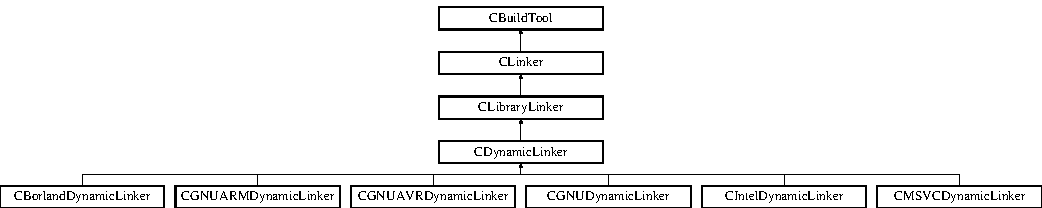
\includegraphics[height=2.794411cm]{d9/d8b/classCDynamicLinker}
\end{center}
\end{figure}
\subsection*{Public Member Functions}
\begin{DoxyCompactItemize}
\item 
virtual \hyperlink{classCDynamicLinker}{C\-Dynamic\-Linker} $\ast$ \hyperlink{classCDynamicLinker_ac71406ca5c6e8e991a6418a6307d274c}{Create\-Instance} (void)
\item 
virtual void \hyperlink{classCDynamicLinker_a437d46ee65b3585e7be9d15d40c26820}{Reset} (const \hyperlink{classCPlatform_a2fb735c63c53052f79629e338bb0f535}{C\-Platform\-::\-O\-S\-\_\-\-Type} O\-S)
\item 
\hyperlink{classCDynamicLinker_a533aff3d7d03c5a568b5a5dd2cbe969d}{C\-Dynamic\-Linker} (void)
\item 
\hyperlink{classCDynamicLinker_ad503d4979209cbcbeb573ef785197034}{C\-Dynamic\-Linker} (const \hyperlink{classCDynamicLinker}{C\-Dynamic\-Linker} \&Dynamic\-Linker)
\item 
virtual \hyperlink{classCDynamicLinker_a9bb607cf2014d3afe81b84974c83940b}{$\sim$\-C\-Dynamic\-Linker} (void)
\end{DoxyCompactItemize}
\subsection*{Additional Inherited Members}


\subsection{Constructor \& Destructor Documentation}
\hypertarget{classCDynamicLinker_a533aff3d7d03c5a568b5a5dd2cbe969d}{\index{C\-Dynamic\-Linker@{C\-Dynamic\-Linker}!C\-Dynamic\-Linker@{C\-Dynamic\-Linker}}
\index{C\-Dynamic\-Linker@{C\-Dynamic\-Linker}!CDynamicLinker@{C\-Dynamic\-Linker}}
\subsubsection[{C\-Dynamic\-Linker}]{\setlength{\rightskip}{0pt plus 5cm}C\-Dynamic\-Linker\-::\-C\-Dynamic\-Linker (
\begin{DoxyParamCaption}
\item[{void}]{}
\end{DoxyParamCaption}
)}}\label{classCDynamicLinker_a533aff3d7d03c5a568b5a5dd2cbe969d}
\hypertarget{classCDynamicLinker_ad503d4979209cbcbeb573ef785197034}{\index{C\-Dynamic\-Linker@{C\-Dynamic\-Linker}!C\-Dynamic\-Linker@{C\-Dynamic\-Linker}}
\index{C\-Dynamic\-Linker@{C\-Dynamic\-Linker}!CDynamicLinker@{C\-Dynamic\-Linker}}
\subsubsection[{C\-Dynamic\-Linker}]{\setlength{\rightskip}{0pt plus 5cm}C\-Dynamic\-Linker\-::\-C\-Dynamic\-Linker (
\begin{DoxyParamCaption}
\item[{const {\bf C\-Dynamic\-Linker} \&}]{Dynamic\-Linker}
\end{DoxyParamCaption}
)}}\label{classCDynamicLinker_ad503d4979209cbcbeb573ef785197034}
\hypertarget{classCDynamicLinker_a9bb607cf2014d3afe81b84974c83940b}{\index{C\-Dynamic\-Linker@{C\-Dynamic\-Linker}!$\sim$\-C\-Dynamic\-Linker@{$\sim$\-C\-Dynamic\-Linker}}
\index{$\sim$\-C\-Dynamic\-Linker@{$\sim$\-C\-Dynamic\-Linker}!CDynamicLinker@{C\-Dynamic\-Linker}}
\subsubsection[{$\sim$\-C\-Dynamic\-Linker}]{\setlength{\rightskip}{0pt plus 5cm}C\-Dynamic\-Linker\-::$\sim$\-C\-Dynamic\-Linker (
\begin{DoxyParamCaption}
\item[{void}]{}
\end{DoxyParamCaption}
)\hspace{0.3cm}{\ttfamily [virtual]}}}\label{classCDynamicLinker_a9bb607cf2014d3afe81b84974c83940b}


\subsection{Member Function Documentation}
\hypertarget{classCDynamicLinker_ac71406ca5c6e8e991a6418a6307d274c}{\index{C\-Dynamic\-Linker@{C\-Dynamic\-Linker}!Create\-Instance@{Create\-Instance}}
\index{Create\-Instance@{Create\-Instance}!CDynamicLinker@{C\-Dynamic\-Linker}}
\subsubsection[{Create\-Instance}]{\setlength{\rightskip}{0pt plus 5cm}{\bf C\-Dynamic\-Linker} $\ast$ C\-Dynamic\-Linker\-::\-Create\-Instance (
\begin{DoxyParamCaption}
\item[{void}]{}
\end{DoxyParamCaption}
)\hspace{0.3cm}{\ttfamily [virtual]}}}\label{classCDynamicLinker_ac71406ca5c6e8e991a6418a6307d274c}


Reimplemented from \hyperlink{classCLibraryLinker_a02b85c6bc81ad2973ee9a578412a1fa0}{C\-Library\-Linker}.



Reimplemented in \hyperlink{classCMSVCDynamicLinker_ad8fc45d290987fb96b9a983b592a2ad1}{C\-M\-S\-V\-C\-Dynamic\-Linker}, \hyperlink{classCIntelDynamicLinker_a51e4c22985b5c518e8cdef1abeee7d85}{C\-Intel\-Dynamic\-Linker}, \hyperlink{classCBorlandDynamicLinker_ae76cbd521d03bd3eee2f1d5fe8836d03}{C\-Borland\-Dynamic\-Linker}, \hyperlink{classCGNUARMDynamicLinker_ad3ded52b8101b6f85ad6d5609f85c78c}{C\-G\-N\-U\-A\-R\-M\-Dynamic\-Linker}, \hyperlink{classCGNUAVRDynamicLinker_ae26802d4ce8ce7c45a87a65bf7066832}{C\-G\-N\-U\-A\-V\-R\-Dynamic\-Linker}, and \hyperlink{classCGNUDynamicLinker_addcaa2506e1f804b4737cb564a899f6c}{C\-G\-N\-U\-Dynamic\-Linker}.

\hypertarget{classCDynamicLinker_a437d46ee65b3585e7be9d15d40c26820}{\index{C\-Dynamic\-Linker@{C\-Dynamic\-Linker}!Reset@{Reset}}
\index{Reset@{Reset}!CDynamicLinker@{C\-Dynamic\-Linker}}
\subsubsection[{Reset}]{\setlength{\rightskip}{0pt plus 5cm}void C\-Dynamic\-Linker\-::\-Reset (
\begin{DoxyParamCaption}
\item[{const {\bf C\-Platform\-::\-O\-S\-\_\-\-Type}}]{O\-S}
\end{DoxyParamCaption}
)\hspace{0.3cm}{\ttfamily [virtual]}}}\label{classCDynamicLinker_a437d46ee65b3585e7be9d15d40c26820}


Reimplemented from \hyperlink{classCBuildTool_abea21a0e61ab2177effdff5aaa169585}{C\-Build\-Tool}.



Reimplemented in \hyperlink{classCMSVCDynamicLinker_aae22160e1bee1d4231ce669ac0132937}{C\-M\-S\-V\-C\-Dynamic\-Linker}, \hyperlink{classCIntelDynamicLinker_a9716e2053535fcadd92d46699d8b445e}{C\-Intel\-Dynamic\-Linker}, \hyperlink{classCBorlandDynamicLinker_acbf22349e7e89873dac5f55f8d9adc8b}{C\-Borland\-Dynamic\-Linker}, \hyperlink{classCGNUARMDynamicLinker_a3f49a2938f97c58d9eaee0986f3b9866}{C\-G\-N\-U\-A\-R\-M\-Dynamic\-Linker}, \hyperlink{classCGNUAVRDynamicLinker_a08c53dfc9f1352a486bfb736aee544f4}{C\-G\-N\-U\-A\-V\-R\-Dynamic\-Linker}, and \hyperlink{classCGNUDynamicLinker_ae156df1627238831556bd40597694d7e}{C\-G\-N\-U\-Dynamic\-Linker}.



The documentation for this class was generated from the following files\-:\begin{DoxyCompactItemize}
\item 
src/\hyperlink{buildtools_8h}{buildtools.\-h}\item 
src/\hyperlink{buildtools_8cpp}{buildtools.\-cpp}\end{DoxyCompactItemize}

\hypertarget{classCExecutableLinker}{\section{C\-Executable\-Linker Class Reference}
\label{classCExecutableLinker}\index{C\-Executable\-Linker@{C\-Executable\-Linker}}
}


{\ttfamily \#include $<$buildtools.\-h$>$}

Inheritance diagram for C\-Executable\-Linker\-:\begin{figure}[H]
\begin{center}
\leavevmode
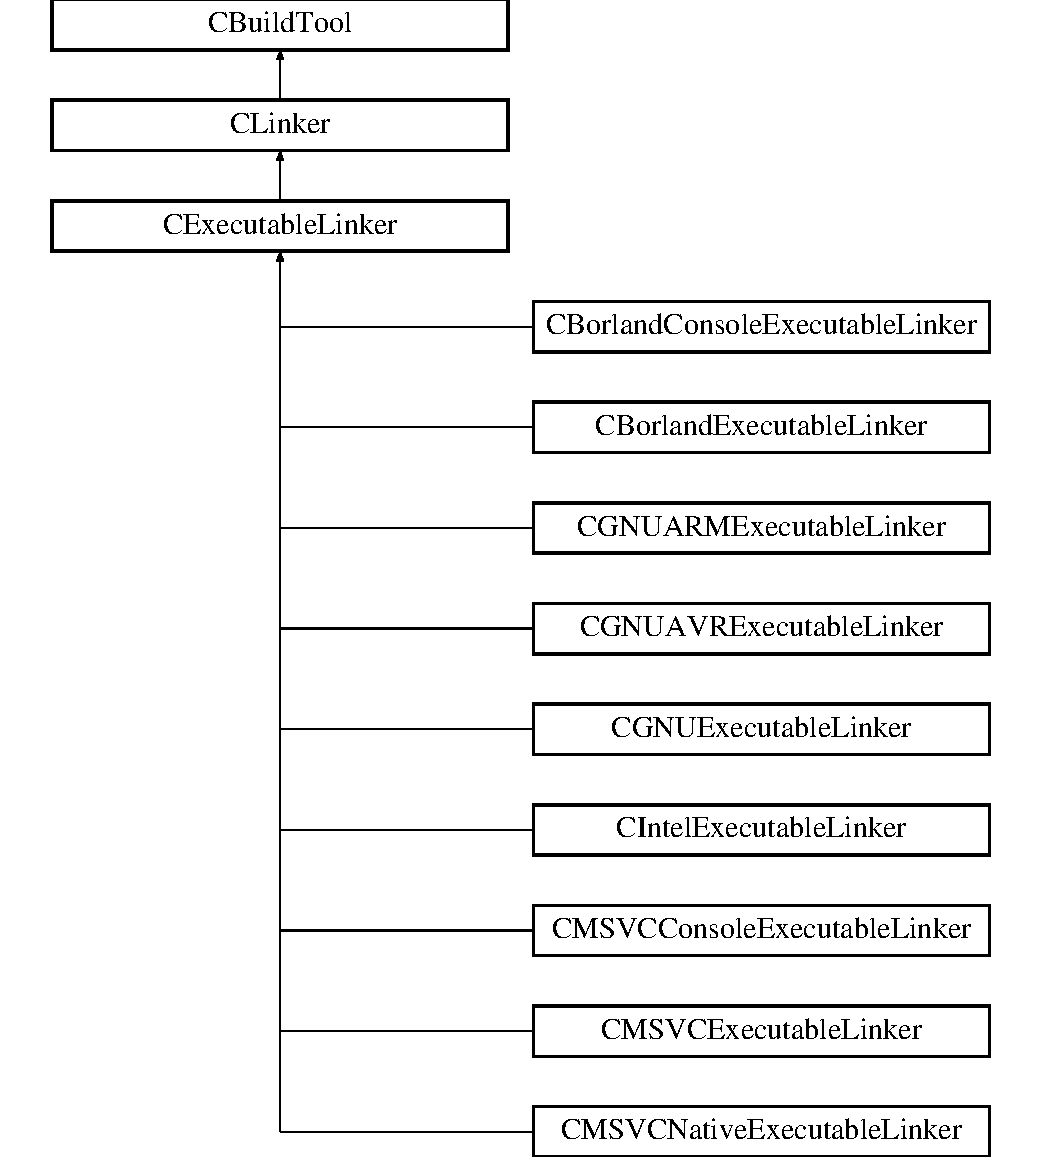
\includegraphics[height=12.000000cm]{d5/d2f/classCExecutableLinker}
\end{center}
\end{figure}
\subsection*{Public Member Functions}
\begin{DoxyCompactItemize}
\item 
virtual \hyperlink{classCExecutableLinker}{C\-Executable\-Linker} $\ast$ \hyperlink{classCExecutableLinker_a457b823b737b0a78285d5ede77df827c}{Create\-Instance} (void)
\item 
\hyperlink{classCString}{C\-String} \hyperlink{classCExecutableLinker_aeb465eef80267304b011425fa9c242a4}{Option\-Win\-G\-U\-I} (void) const 
\item 
virtual void \hyperlink{classCExecutableLinker_a181ea374618a85985db14f468dc63023}{Read} (const Ti\-Xml\-Element $\ast$Build\-Tool\-Root)
\item 
virtual void \hyperlink{classCExecutableLinker_a6124deba72724510423c17963f960578}{Write} (Ti\-Xml\-Element $\ast$Build\-Tool\-Root)
\item 
virtual void \hyperlink{classCExecutableLinker_a01fa91b454c4cc4d154a26f0ab8da467}{Show} (void)
\item 
\hyperlink{classCExecutableLinker_a12713b324a534deaf474afa0732e11e5}{C\-Executable\-Linker} (void)
\item 
\hyperlink{classCExecutableLinker_aea030dc919cbc3f4ce2bce840471d927}{C\-Executable\-Linker} (const \hyperlink{classCExecutableLinker}{C\-Executable\-Linker} \&Executable\-Linker)
\item 
virtual \hyperlink{classCExecutableLinker_a5418dd890762573a7b9273f3bbdc3ef7}{$\sim$\-C\-Executable\-Linker} (void)
\end{DoxyCompactItemize}
\subsection*{Protected Attributes}
\begin{DoxyCompactItemize}
\item 
\hyperlink{classCString}{C\-String} \hyperlink{classCExecutableLinker_adff4da821e3b71b39b84f5ea5d183f87}{m\-\_\-\-Option\-\_\-\-Win\-G\-U\-I}
\end{DoxyCompactItemize}
\subsection*{Additional Inherited Members}


\subsection{Constructor \& Destructor Documentation}
\hypertarget{classCExecutableLinker_a12713b324a534deaf474afa0732e11e5}{\index{C\-Executable\-Linker@{C\-Executable\-Linker}!C\-Executable\-Linker@{C\-Executable\-Linker}}
\index{C\-Executable\-Linker@{C\-Executable\-Linker}!CExecutableLinker@{C\-Executable\-Linker}}
\subsubsection[{C\-Executable\-Linker}]{\setlength{\rightskip}{0pt plus 5cm}C\-Executable\-Linker\-::\-C\-Executable\-Linker (
\begin{DoxyParamCaption}
\item[{void}]{}
\end{DoxyParamCaption}
)}}\label{classCExecutableLinker_a12713b324a534deaf474afa0732e11e5}
\hypertarget{classCExecutableLinker_aea030dc919cbc3f4ce2bce840471d927}{\index{C\-Executable\-Linker@{C\-Executable\-Linker}!C\-Executable\-Linker@{C\-Executable\-Linker}}
\index{C\-Executable\-Linker@{C\-Executable\-Linker}!CExecutableLinker@{C\-Executable\-Linker}}
\subsubsection[{C\-Executable\-Linker}]{\setlength{\rightskip}{0pt plus 5cm}C\-Executable\-Linker\-::\-C\-Executable\-Linker (
\begin{DoxyParamCaption}
\item[{const {\bf C\-Executable\-Linker} \&}]{Executable\-Linker}
\end{DoxyParamCaption}
)}}\label{classCExecutableLinker_aea030dc919cbc3f4ce2bce840471d927}
\hypertarget{classCExecutableLinker_a5418dd890762573a7b9273f3bbdc3ef7}{\index{C\-Executable\-Linker@{C\-Executable\-Linker}!$\sim$\-C\-Executable\-Linker@{$\sim$\-C\-Executable\-Linker}}
\index{$\sim$\-C\-Executable\-Linker@{$\sim$\-C\-Executable\-Linker}!CExecutableLinker@{C\-Executable\-Linker}}
\subsubsection[{$\sim$\-C\-Executable\-Linker}]{\setlength{\rightskip}{0pt plus 5cm}C\-Executable\-Linker\-::$\sim$\-C\-Executable\-Linker (
\begin{DoxyParamCaption}
\item[{void}]{}
\end{DoxyParamCaption}
)\hspace{0.3cm}{\ttfamily [virtual]}}}\label{classCExecutableLinker_a5418dd890762573a7b9273f3bbdc3ef7}


\subsection{Member Function Documentation}
\hypertarget{classCExecutableLinker_a457b823b737b0a78285d5ede77df827c}{\index{C\-Executable\-Linker@{C\-Executable\-Linker}!Create\-Instance@{Create\-Instance}}
\index{Create\-Instance@{Create\-Instance}!CExecutableLinker@{C\-Executable\-Linker}}
\subsubsection[{Create\-Instance}]{\setlength{\rightskip}{0pt plus 5cm}{\bf C\-Executable\-Linker} $\ast$ C\-Executable\-Linker\-::\-Create\-Instance (
\begin{DoxyParamCaption}
\item[{void}]{}
\end{DoxyParamCaption}
)\hspace{0.3cm}{\ttfamily [virtual]}}}\label{classCExecutableLinker_a457b823b737b0a78285d5ede77df827c}


Reimplemented from \hyperlink{classCLinker_a9b644b9c906436f75b394f2324d811d3}{C\-Linker}.



Reimplemented in \hyperlink{classCMSVCNativeExecutableLinker_ab769242f54c4336e1cedd340b8a45d3a}{C\-M\-S\-V\-C\-Native\-Executable\-Linker}, \hyperlink{classCMSVCConsoleExecutableLinker_a9240460d8f7ea9651177279bf0640a88}{C\-M\-S\-V\-C\-Console\-Executable\-Linker}, \hyperlink{classCMSVCExecutableLinker_ad5b1391fa863f9e966562ee227a00693}{C\-M\-S\-V\-C\-Executable\-Linker}, \hyperlink{classCIntelExecutableLinker_aacec1bc57c88a614c449a6873c1cc489}{C\-Intel\-Executable\-Linker}, \hyperlink{classCBorlandConsoleExecutableLinker_a1aba394784a724a2b59c021b732484f8}{C\-Borland\-Console\-Executable\-Linker}, \hyperlink{classCBorlandExecutableLinker_ab4acecd477ed0458760a3f14ee6fb868}{C\-Borland\-Executable\-Linker}, \hyperlink{classCGNUARMExecutableLinker_a9241ead8113a3c4c3820240f3993fb19}{C\-G\-N\-U\-A\-R\-M\-Executable\-Linker}, \hyperlink{classCGNUAVRExecutableLinker_ad6c7693277ecb00d550bde8e1bda0b8c}{C\-G\-N\-U\-A\-V\-R\-Executable\-Linker}, and \hyperlink{classCGNUExecutableLinker_a96d5c82ab5c7c26e7e9ef1542c815e94}{C\-G\-N\-U\-Executable\-Linker}.

\hypertarget{classCExecutableLinker_aeb465eef80267304b011425fa9c242a4}{\index{C\-Executable\-Linker@{C\-Executable\-Linker}!Option\-Win\-G\-U\-I@{Option\-Win\-G\-U\-I}}
\index{Option\-Win\-G\-U\-I@{Option\-Win\-G\-U\-I}!CExecutableLinker@{C\-Executable\-Linker}}
\subsubsection[{Option\-Win\-G\-U\-I}]{\setlength{\rightskip}{0pt plus 5cm}{\bf C\-String} C\-Executable\-Linker\-::\-Option\-Win\-G\-U\-I (
\begin{DoxyParamCaption}
\item[{void}]{}
\end{DoxyParamCaption}
) const\hspace{0.3cm}{\ttfamily [inline]}}}\label{classCExecutableLinker_aeb465eef80267304b011425fa9c242a4}
\hypertarget{classCExecutableLinker_a181ea374618a85985db14f468dc63023}{\index{C\-Executable\-Linker@{C\-Executable\-Linker}!Read@{Read}}
\index{Read@{Read}!CExecutableLinker@{C\-Executable\-Linker}}
\subsubsection[{Read}]{\setlength{\rightskip}{0pt plus 5cm}void C\-Executable\-Linker\-::\-Read (
\begin{DoxyParamCaption}
\item[{const Ti\-Xml\-Element $\ast$}]{Build\-Tool\-Root}
\end{DoxyParamCaption}
)\hspace{0.3cm}{\ttfamily [virtual]}}}\label{classCExecutableLinker_a181ea374618a85985db14f468dc63023}


Reimplemented from \hyperlink{classCLinker_a6db5ff1a933b56855b2bfb9260f46dce}{C\-Linker}.

\hypertarget{classCExecutableLinker_a01fa91b454c4cc4d154a26f0ab8da467}{\index{C\-Executable\-Linker@{C\-Executable\-Linker}!Show@{Show}}
\index{Show@{Show}!CExecutableLinker@{C\-Executable\-Linker}}
\subsubsection[{Show}]{\setlength{\rightskip}{0pt plus 5cm}void C\-Executable\-Linker\-::\-Show (
\begin{DoxyParamCaption}
\item[{void}]{}
\end{DoxyParamCaption}
)\hspace{0.3cm}{\ttfamily [virtual]}}}\label{classCExecutableLinker_a01fa91b454c4cc4d154a26f0ab8da467}


Reimplemented from \hyperlink{classCLinker_aa2c99f02f4433dfae7cdc0654b901582}{C\-Linker}.

\hypertarget{classCExecutableLinker_a6124deba72724510423c17963f960578}{\index{C\-Executable\-Linker@{C\-Executable\-Linker}!Write@{Write}}
\index{Write@{Write}!CExecutableLinker@{C\-Executable\-Linker}}
\subsubsection[{Write}]{\setlength{\rightskip}{0pt plus 5cm}void C\-Executable\-Linker\-::\-Write (
\begin{DoxyParamCaption}
\item[{Ti\-Xml\-Element $\ast$}]{Build\-Tool\-Root}
\end{DoxyParamCaption}
)\hspace{0.3cm}{\ttfamily [virtual]}}}\label{classCExecutableLinker_a6124deba72724510423c17963f960578}


Reimplemented from \hyperlink{classCLinker_ad2b70ef5f824d2697b4f12579415dca3}{C\-Linker}.



\subsection{Member Data Documentation}
\hypertarget{classCExecutableLinker_adff4da821e3b71b39b84f5ea5d183f87}{\index{C\-Executable\-Linker@{C\-Executable\-Linker}!m\-\_\-\-Option\-\_\-\-Win\-G\-U\-I@{m\-\_\-\-Option\-\_\-\-Win\-G\-U\-I}}
\index{m\-\_\-\-Option\-\_\-\-Win\-G\-U\-I@{m\-\_\-\-Option\-\_\-\-Win\-G\-U\-I}!CExecutableLinker@{C\-Executable\-Linker}}
\subsubsection[{m\-\_\-\-Option\-\_\-\-Win\-G\-U\-I}]{\setlength{\rightskip}{0pt plus 5cm}{\bf C\-String} C\-Executable\-Linker\-::m\-\_\-\-Option\-\_\-\-Win\-G\-U\-I\hspace{0.3cm}{\ttfamily [protected]}}}\label{classCExecutableLinker_adff4da821e3b71b39b84f5ea5d183f87}


The documentation for this class was generated from the following files\-:\begin{DoxyCompactItemize}
\item 
src/\hyperlink{buildtools_8h}{buildtools.\-h}\item 
src/\hyperlink{buildtools_8cpp}{buildtools.\-cpp}\end{DoxyCompactItemize}

\hypertarget{classCFloatVariable}{\section{C\-Float\-Variable Class Reference}
\label{classCFloatVariable}\index{C\-Float\-Variable@{C\-Float\-Variable}}
}


{\ttfamily \#include $<$stlvariables.\-h$>$}

Inheritance diagram for C\-Float\-Variable\-:\begin{figure}[H]
\begin{center}
\leavevmode
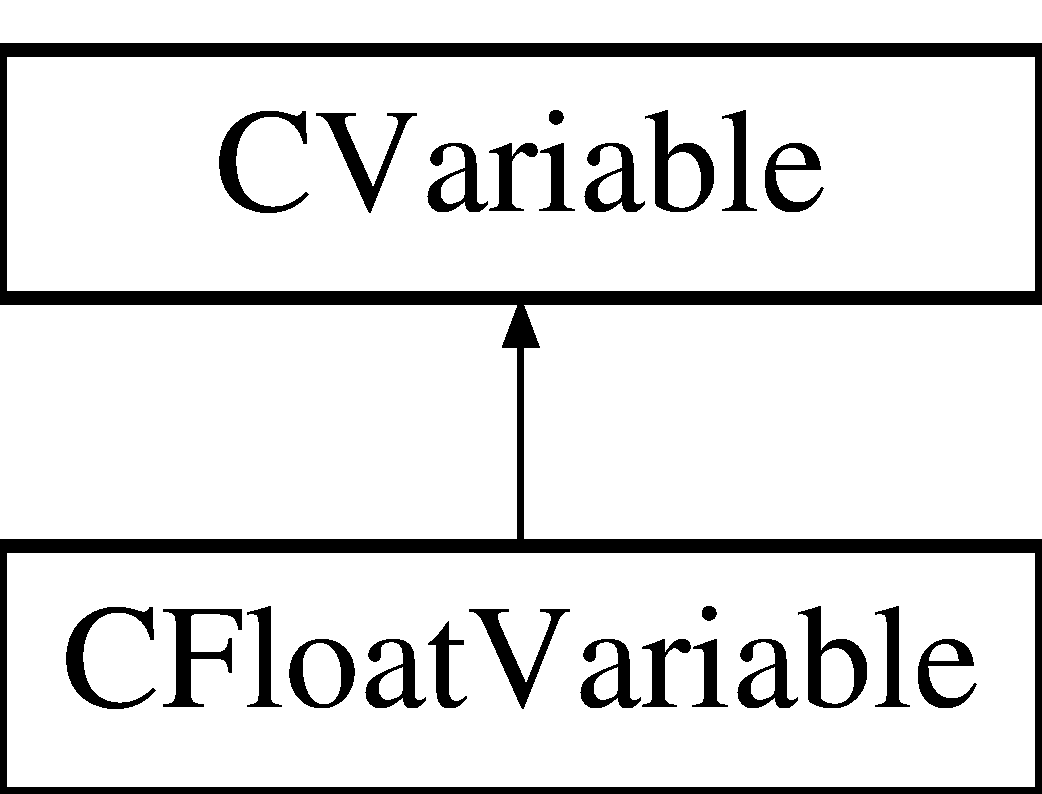
\includegraphics[height=2.000000cm]{d3/dca/classCFloatVariable}
\end{center}
\end{figure}
\subsection*{Public Member Functions}
\begin{DoxyCompactItemize}
\item 
virtual int \hyperlink{classCFloatVariable_acd359d977869758d423ad207c108eaa7}{Get\-Type} (void) const 
\item 
virtual \hyperlink{classCString}{C\-String} \hyperlink{classCFloatVariable_a0b28d738f0395143ae5ebca6b5ed19a2}{Get\-Type\-Name} (void) const 
\item 
virtual double \hyperlink{classCFloatVariable_ae591dcf958100c9702162ae4335f7589}{Get\-Float} (void) const 
\item 
virtual void \hyperlink{classCFloatVariable_ae7e6889263d0d1e6199fc814109e2049}{Set\-Float} (const double Value)
\item 
virtual int \hyperlink{classCFloatVariable_a7a6d456bfb26f4e008e8dfc9db480a03}{Get\-Integer} (void) const 
\item 
virtual void \hyperlink{classCFloatVariable_ad6b19217796d4817cfde059b03e57a9b}{Set\-Integer} (const int Value)
\item 
virtual bool \hyperlink{classCFloatVariable_af662cca772ad13969a23f4dc78af38ea}{Get\-Boolean} (void) const 
\item 
virtual void \hyperlink{classCFloatVariable_a767ea025e89f033e1ba6e98b5c967691}{Set\-Boolean} (const bool Value)
\item 
virtual \hyperlink{classCString}{C\-String} \hyperlink{classCFloatVariable_a7aa60c5828e23145adec0cd6116e5d41}{Get\-String} (void) const 
\item 
virtual void \hyperlink{classCFloatVariable_a413448c60d1be13e1b28ea4e56733abc}{Set\-String} (const \hyperlink{classCString}{C\-String} \&Value)
\item 
virtual char \hyperlink{classCFloatVariable_ab9cc3930a0c138a2e198c6d0e8f3626c}{Get\-Char} (void) const 
\item 
virtual void \hyperlink{classCFloatVariable_acc613e2a2897e2e45c9b666c8ea8ae2a}{Set\-Char} (const char Value)
\item 
double \hyperlink{classCFloatVariable_a7b4b14c140e201a1c0b42631c29235d4}{operator=} (const \hyperlink{classCFloatVariable}{C\-Float\-Variable} \&Variable)
\item 
\hyperlink{classCFloatVariable}{C\-Float\-Variable} \& \hyperlink{classCFloatVariable_a4ef005421df21170149a87b70c6a61b6}{operator=} (const double Value)
\item 
\hyperlink{classCFloatVariable}{C\-Float\-Variable} \& \hyperlink{classCFloatVariable_a262cf84d4b36a6632a79fd147cedc743}{operator=} (const int Value)
\item 
\hyperlink{classCFloatVariable}{C\-Float\-Variable} \& \hyperlink{classCFloatVariable_ae093d9e1bcc2322935e581573686f6d0}{operator=} (const bool Value)
\item 
\hyperlink{classCFloatVariable}{C\-Float\-Variable} \& \hyperlink{classCFloatVariable_a5734706330eef91580b2bbfa9ed139e5}{operator=} (const \hyperlink{classCString}{C\-String} \&Value)
\item 
\hyperlink{classCFloatVariable}{C\-Float\-Variable} \& \hyperlink{classCFloatVariable_af60a68bcc968297b8221f34332089497}{operator=} (const char Value)
\item 
\hyperlink{classCFloatVariable_a4edea7981c2f4d19f98e8227181dff73}{C\-Float\-Variable} (const \hyperlink{classCString}{C\-String} \&Name, const double Value=0.\-0)
\item 
virtual \hyperlink{classCFloatVariable_a340049936766ef7db8653df3ecec1c19}{$\sim$\-C\-Float\-Variable} (void)
\end{DoxyCompactItemize}
\subsection*{Protected Attributes}
\begin{DoxyCompactItemize}
\item 
double \hyperlink{classCFloatVariable_aa25bca6796483d1055947eceb2aff411}{m\-\_\-\-Value}
\end{DoxyCompactItemize}


\subsection{Constructor \& Destructor Documentation}
\hypertarget{classCFloatVariable_a4edea7981c2f4d19f98e8227181dff73}{\index{C\-Float\-Variable@{C\-Float\-Variable}!C\-Float\-Variable@{C\-Float\-Variable}}
\index{C\-Float\-Variable@{C\-Float\-Variable}!CFloatVariable@{C\-Float\-Variable}}
\subsubsection[{C\-Float\-Variable}]{\setlength{\rightskip}{0pt plus 5cm}C\-Float\-Variable\-::\-C\-Float\-Variable (
\begin{DoxyParamCaption}
\item[{const {\bf C\-String} \&}]{Name, }
\item[{const double}]{Value = {\ttfamily 0.0}}
\end{DoxyParamCaption}
)}}\label{classCFloatVariable_a4edea7981c2f4d19f98e8227181dff73}
\hypertarget{classCFloatVariable_a340049936766ef7db8653df3ecec1c19}{\index{C\-Float\-Variable@{C\-Float\-Variable}!$\sim$\-C\-Float\-Variable@{$\sim$\-C\-Float\-Variable}}
\index{$\sim$\-C\-Float\-Variable@{$\sim$\-C\-Float\-Variable}!CFloatVariable@{C\-Float\-Variable}}
\subsubsection[{$\sim$\-C\-Float\-Variable}]{\setlength{\rightskip}{0pt plus 5cm}virtual C\-Float\-Variable\-::$\sim$\-C\-Float\-Variable (
\begin{DoxyParamCaption}
\item[{void}]{}
\end{DoxyParamCaption}
)\hspace{0.3cm}{\ttfamily [inline]}, {\ttfamily [virtual]}}}\label{classCFloatVariable_a340049936766ef7db8653df3ecec1c19}


\subsection{Member Function Documentation}
\hypertarget{classCFloatVariable_af662cca772ad13969a23f4dc78af38ea}{\index{C\-Float\-Variable@{C\-Float\-Variable}!Get\-Boolean@{Get\-Boolean}}
\index{Get\-Boolean@{Get\-Boolean}!CFloatVariable@{C\-Float\-Variable}}
\subsubsection[{Get\-Boolean}]{\setlength{\rightskip}{0pt plus 5cm}bool C\-Float\-Variable\-::\-Get\-Boolean (
\begin{DoxyParamCaption}
\item[{void}]{}
\end{DoxyParamCaption}
) const\hspace{0.3cm}{\ttfamily [virtual]}}}\label{classCFloatVariable_af662cca772ad13969a23f4dc78af38ea}


Reimplemented from \hyperlink{classCVariable_a874156d6b1a3a44f799c32a2455c7f49}{C\-Variable}.

\hypertarget{classCFloatVariable_ab9cc3930a0c138a2e198c6d0e8f3626c}{\index{C\-Float\-Variable@{C\-Float\-Variable}!Get\-Char@{Get\-Char}}
\index{Get\-Char@{Get\-Char}!CFloatVariable@{C\-Float\-Variable}}
\subsubsection[{Get\-Char}]{\setlength{\rightskip}{0pt plus 5cm}char C\-Float\-Variable\-::\-Get\-Char (
\begin{DoxyParamCaption}
\item[{void}]{}
\end{DoxyParamCaption}
) const\hspace{0.3cm}{\ttfamily [virtual]}}}\label{classCFloatVariable_ab9cc3930a0c138a2e198c6d0e8f3626c}


Reimplemented from \hyperlink{classCVariable_a6635a8fd2441dcb83a39d10a78187dac}{C\-Variable}.

\hypertarget{classCFloatVariable_ae591dcf958100c9702162ae4335f7589}{\index{C\-Float\-Variable@{C\-Float\-Variable}!Get\-Float@{Get\-Float}}
\index{Get\-Float@{Get\-Float}!CFloatVariable@{C\-Float\-Variable}}
\subsubsection[{Get\-Float}]{\setlength{\rightskip}{0pt plus 5cm}double C\-Float\-Variable\-::\-Get\-Float (
\begin{DoxyParamCaption}
\item[{void}]{}
\end{DoxyParamCaption}
) const\hspace{0.3cm}{\ttfamily [virtual]}}}\label{classCFloatVariable_ae591dcf958100c9702162ae4335f7589}


Reimplemented from \hyperlink{classCVariable_ac475ad87ffbfaeeb2d4d9c2986b0d575}{C\-Variable}.

\hypertarget{classCFloatVariable_a7a6d456bfb26f4e008e8dfc9db480a03}{\index{C\-Float\-Variable@{C\-Float\-Variable}!Get\-Integer@{Get\-Integer}}
\index{Get\-Integer@{Get\-Integer}!CFloatVariable@{C\-Float\-Variable}}
\subsubsection[{Get\-Integer}]{\setlength{\rightskip}{0pt plus 5cm}int C\-Float\-Variable\-::\-Get\-Integer (
\begin{DoxyParamCaption}
\item[{void}]{}
\end{DoxyParamCaption}
) const\hspace{0.3cm}{\ttfamily [virtual]}}}\label{classCFloatVariable_a7a6d456bfb26f4e008e8dfc9db480a03}


Reimplemented from \hyperlink{classCVariable_adb0db49f4a55f3e1b5322f6ce26e4ebc}{C\-Variable}.

\hypertarget{classCFloatVariable_a7aa60c5828e23145adec0cd6116e5d41}{\index{C\-Float\-Variable@{C\-Float\-Variable}!Get\-String@{Get\-String}}
\index{Get\-String@{Get\-String}!CFloatVariable@{C\-Float\-Variable}}
\subsubsection[{Get\-String}]{\setlength{\rightskip}{0pt plus 5cm}{\bf C\-String} C\-Float\-Variable\-::\-Get\-String (
\begin{DoxyParamCaption}
\item[{void}]{}
\end{DoxyParamCaption}
) const\hspace{0.3cm}{\ttfamily [virtual]}}}\label{classCFloatVariable_a7aa60c5828e23145adec0cd6116e5d41}


Reimplemented from \hyperlink{classCVariable_aefa25c880c0042ffc29889475d329004}{C\-Variable}.

\hypertarget{classCFloatVariable_acd359d977869758d423ad207c108eaa7}{\index{C\-Float\-Variable@{C\-Float\-Variable}!Get\-Type@{Get\-Type}}
\index{Get\-Type@{Get\-Type}!CFloatVariable@{C\-Float\-Variable}}
\subsubsection[{Get\-Type}]{\setlength{\rightskip}{0pt plus 5cm}int C\-Float\-Variable\-::\-Get\-Type (
\begin{DoxyParamCaption}
\item[{void}]{}
\end{DoxyParamCaption}
) const\hspace{0.3cm}{\ttfamily [virtual]}}}\label{classCFloatVariable_acd359d977869758d423ad207c108eaa7}


Reimplemented from \hyperlink{classCVariable_acdf7301ad2f5c7fa33770c028211c0bc}{C\-Variable}.

\hypertarget{classCFloatVariable_a0b28d738f0395143ae5ebca6b5ed19a2}{\index{C\-Float\-Variable@{C\-Float\-Variable}!Get\-Type\-Name@{Get\-Type\-Name}}
\index{Get\-Type\-Name@{Get\-Type\-Name}!CFloatVariable@{C\-Float\-Variable}}
\subsubsection[{Get\-Type\-Name}]{\setlength{\rightskip}{0pt plus 5cm}{\bf C\-String} C\-Float\-Variable\-::\-Get\-Type\-Name (
\begin{DoxyParamCaption}
\item[{void}]{}
\end{DoxyParamCaption}
) const\hspace{0.3cm}{\ttfamily [virtual]}}}\label{classCFloatVariable_a0b28d738f0395143ae5ebca6b5ed19a2}


Reimplemented from \hyperlink{classCVariable_ad8a23d1501917cbfb1eee1473a7a2122}{C\-Variable}.

\hypertarget{classCFloatVariable_a7b4b14c140e201a1c0b42631c29235d4}{\index{C\-Float\-Variable@{C\-Float\-Variable}!operator=@{operator=}}
\index{operator=@{operator=}!CFloatVariable@{C\-Float\-Variable}}
\subsubsection[{operator=}]{\setlength{\rightskip}{0pt plus 5cm}double C\-Float\-Variable\-::operator= (
\begin{DoxyParamCaption}
\item[{const {\bf C\-Float\-Variable} \&}]{Variable}
\end{DoxyParamCaption}
)}}\label{classCFloatVariable_a7b4b14c140e201a1c0b42631c29235d4}
\hypertarget{classCFloatVariable_a4ef005421df21170149a87b70c6a61b6}{\index{C\-Float\-Variable@{C\-Float\-Variable}!operator=@{operator=}}
\index{operator=@{operator=}!CFloatVariable@{C\-Float\-Variable}}
\subsubsection[{operator=}]{\setlength{\rightskip}{0pt plus 5cm}{\bf C\-Float\-Variable} \& C\-Float\-Variable\-::operator= (
\begin{DoxyParamCaption}
\item[{const double}]{Value}
\end{DoxyParamCaption}
)}}\label{classCFloatVariable_a4ef005421df21170149a87b70c6a61b6}
\hypertarget{classCFloatVariable_a262cf84d4b36a6632a79fd147cedc743}{\index{C\-Float\-Variable@{C\-Float\-Variable}!operator=@{operator=}}
\index{operator=@{operator=}!CFloatVariable@{C\-Float\-Variable}}
\subsubsection[{operator=}]{\setlength{\rightskip}{0pt plus 5cm}{\bf C\-Float\-Variable} \& C\-Float\-Variable\-::operator= (
\begin{DoxyParamCaption}
\item[{const int}]{Value}
\end{DoxyParamCaption}
)}}\label{classCFloatVariable_a262cf84d4b36a6632a79fd147cedc743}
\hypertarget{classCFloatVariable_ae093d9e1bcc2322935e581573686f6d0}{\index{C\-Float\-Variable@{C\-Float\-Variable}!operator=@{operator=}}
\index{operator=@{operator=}!CFloatVariable@{C\-Float\-Variable}}
\subsubsection[{operator=}]{\setlength{\rightskip}{0pt plus 5cm}{\bf C\-Float\-Variable} \& C\-Float\-Variable\-::operator= (
\begin{DoxyParamCaption}
\item[{const bool}]{Value}
\end{DoxyParamCaption}
)}}\label{classCFloatVariable_ae093d9e1bcc2322935e581573686f6d0}
\hypertarget{classCFloatVariable_a5734706330eef91580b2bbfa9ed139e5}{\index{C\-Float\-Variable@{C\-Float\-Variable}!operator=@{operator=}}
\index{operator=@{operator=}!CFloatVariable@{C\-Float\-Variable}}
\subsubsection[{operator=}]{\setlength{\rightskip}{0pt plus 5cm}{\bf C\-Float\-Variable} \& C\-Float\-Variable\-::operator= (
\begin{DoxyParamCaption}
\item[{const {\bf C\-String} \&}]{Value}
\end{DoxyParamCaption}
)}}\label{classCFloatVariable_a5734706330eef91580b2bbfa9ed139e5}
\hypertarget{classCFloatVariable_af60a68bcc968297b8221f34332089497}{\index{C\-Float\-Variable@{C\-Float\-Variable}!operator=@{operator=}}
\index{operator=@{operator=}!CFloatVariable@{C\-Float\-Variable}}
\subsubsection[{operator=}]{\setlength{\rightskip}{0pt plus 5cm}{\bf C\-Float\-Variable} \& C\-Float\-Variable\-::operator= (
\begin{DoxyParamCaption}
\item[{const char}]{Value}
\end{DoxyParamCaption}
)}}\label{classCFloatVariable_af60a68bcc968297b8221f34332089497}
\hypertarget{classCFloatVariable_a767ea025e89f033e1ba6e98b5c967691}{\index{C\-Float\-Variable@{C\-Float\-Variable}!Set\-Boolean@{Set\-Boolean}}
\index{Set\-Boolean@{Set\-Boolean}!CFloatVariable@{C\-Float\-Variable}}
\subsubsection[{Set\-Boolean}]{\setlength{\rightskip}{0pt plus 5cm}void C\-Float\-Variable\-::\-Set\-Boolean (
\begin{DoxyParamCaption}
\item[{const bool}]{Value}
\end{DoxyParamCaption}
)\hspace{0.3cm}{\ttfamily [virtual]}}}\label{classCFloatVariable_a767ea025e89f033e1ba6e98b5c967691}


Reimplemented from \hyperlink{classCVariable_a5c8d2cb9ae53c01dc1ec7e45f8903126}{C\-Variable}.

\hypertarget{classCFloatVariable_acc613e2a2897e2e45c9b666c8ea8ae2a}{\index{C\-Float\-Variable@{C\-Float\-Variable}!Set\-Char@{Set\-Char}}
\index{Set\-Char@{Set\-Char}!CFloatVariable@{C\-Float\-Variable}}
\subsubsection[{Set\-Char}]{\setlength{\rightskip}{0pt plus 5cm}void C\-Float\-Variable\-::\-Set\-Char (
\begin{DoxyParamCaption}
\item[{const char}]{Value}
\end{DoxyParamCaption}
)\hspace{0.3cm}{\ttfamily [virtual]}}}\label{classCFloatVariable_acc613e2a2897e2e45c9b666c8ea8ae2a}


Reimplemented from \hyperlink{classCVariable_a10a96343a4a2437b02b7105adf87a64c}{C\-Variable}.

\hypertarget{classCFloatVariable_ae7e6889263d0d1e6199fc814109e2049}{\index{C\-Float\-Variable@{C\-Float\-Variable}!Set\-Float@{Set\-Float}}
\index{Set\-Float@{Set\-Float}!CFloatVariable@{C\-Float\-Variable}}
\subsubsection[{Set\-Float}]{\setlength{\rightskip}{0pt plus 5cm}void C\-Float\-Variable\-::\-Set\-Float (
\begin{DoxyParamCaption}
\item[{const double}]{Value}
\end{DoxyParamCaption}
)\hspace{0.3cm}{\ttfamily [virtual]}}}\label{classCFloatVariable_ae7e6889263d0d1e6199fc814109e2049}


Reimplemented from \hyperlink{classCVariable_ae352cd2c25541c1137b0f12926d09995}{C\-Variable}.

\hypertarget{classCFloatVariable_ad6b19217796d4817cfde059b03e57a9b}{\index{C\-Float\-Variable@{C\-Float\-Variable}!Set\-Integer@{Set\-Integer}}
\index{Set\-Integer@{Set\-Integer}!CFloatVariable@{C\-Float\-Variable}}
\subsubsection[{Set\-Integer}]{\setlength{\rightskip}{0pt plus 5cm}void C\-Float\-Variable\-::\-Set\-Integer (
\begin{DoxyParamCaption}
\item[{const int}]{Value}
\end{DoxyParamCaption}
)\hspace{0.3cm}{\ttfamily [virtual]}}}\label{classCFloatVariable_ad6b19217796d4817cfde059b03e57a9b}


Reimplemented from \hyperlink{classCVariable_ab97d7164ed35ca67d4bacaebbc7f6fe6}{C\-Variable}.

\hypertarget{classCFloatVariable_a413448c60d1be13e1b28ea4e56733abc}{\index{C\-Float\-Variable@{C\-Float\-Variable}!Set\-String@{Set\-String}}
\index{Set\-String@{Set\-String}!CFloatVariable@{C\-Float\-Variable}}
\subsubsection[{Set\-String}]{\setlength{\rightskip}{0pt plus 5cm}void C\-Float\-Variable\-::\-Set\-String (
\begin{DoxyParamCaption}
\item[{const {\bf C\-String} \&}]{Value}
\end{DoxyParamCaption}
)\hspace{0.3cm}{\ttfamily [virtual]}}}\label{classCFloatVariable_a413448c60d1be13e1b28ea4e56733abc}


Reimplemented from \hyperlink{classCVariable_a7c536a5709d8df5d9d75013370288c79}{C\-Variable}.



\subsection{Member Data Documentation}
\hypertarget{classCFloatVariable_aa25bca6796483d1055947eceb2aff411}{\index{C\-Float\-Variable@{C\-Float\-Variable}!m\-\_\-\-Value@{m\-\_\-\-Value}}
\index{m\-\_\-\-Value@{m\-\_\-\-Value}!CFloatVariable@{C\-Float\-Variable}}
\subsubsection[{m\-\_\-\-Value}]{\setlength{\rightskip}{0pt plus 5cm}double C\-Float\-Variable\-::m\-\_\-\-Value\hspace{0.3cm}{\ttfamily [protected]}}}\label{classCFloatVariable_aa25bca6796483d1055947eceb2aff411}


The documentation for this class was generated from the following files\-:\begin{DoxyCompactItemize}
\item 
lib/\hyperlink{stlvariables_8h}{stlvariables.\-h}\item 
lib/\hyperlink{stlvariables_8cpp}{stlvariables.\-cpp}\end{DoxyCompactItemize}

\hypertarget{classCGenericProcessingMachine}{\section{C\-Generic\-Processing\-Machine Class Reference}
\label{classCGenericProcessingMachine}\index{C\-Generic\-Processing\-Machine@{C\-Generic\-Processing\-Machine}}
}


{\ttfamily \#include $<$stlgpm.\-h$>$}

Inheritance diagram for C\-Generic\-Processing\-Machine\-:\begin{figure}[H]
\begin{center}
\leavevmode
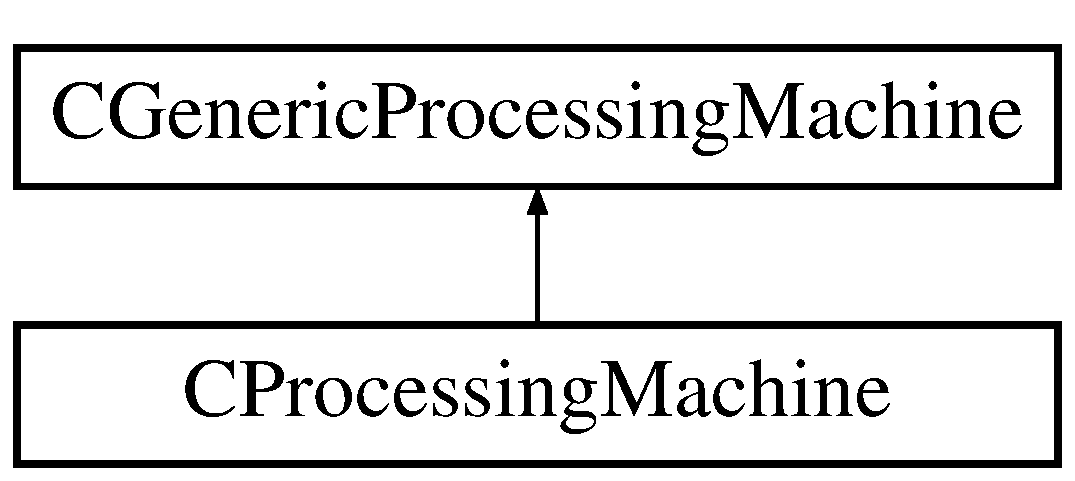
\includegraphics[height=2.000000cm]{d8/dad/classCGenericProcessingMachine}
\end{center}
\end{figure}
\subsection*{Public Member Functions}
\begin{DoxyCompactItemize}
\item 
virtual void \hyperlink{classCGenericProcessingMachine_afc235cd3526341dd66bca63c8407dc3c}{Initialize} (int argc, char $\ast$argv\mbox{[}$\,$\mbox{]})
\item 
virtual void \hyperlink{classCGenericProcessingMachine_a832d5bca8017ae54ee14512d191a0f98}{Initialize} (const \hyperlink{classCParameterString}{C\-Parameter\-String} \&Parameters)
\item 
virtual void \hyperlink{classCGenericProcessingMachine_a220ce336197f41945ed37456b93096bc}{Display\-Help\-Message} (void)
\item 
virtual void \hyperlink{classCGenericProcessingMachine_acfda68ec21cce38d4e43f97e8767da86}{Create\-Configuration} (void)
\item 
\hyperlink{classCString}{C\-String} \hyperlink{classCGenericProcessingMachine_aacfb22cb01d6483a4766907b26decf9b}{Default\-Configuration\-Name} (void)
\item 
virtual \hyperlink{classCString}{C\-String} \hyperlink{classCGenericProcessingMachine_a9f87aeb8f9d4385b054517df3fc4f461}{Configuration\-Name} (void)
\item 
virtual bool \hyperlink{classCGenericProcessingMachine_ab349d35ea588dc0f553906007fdb896b}{Configure} (const \hyperlink{classCString}{C\-String} \&File\-Name)
\item 
int \hyperlink{classCGenericProcessingMachine_a0fe668211df305ffdab90db502ef97b2}{Get\-File\-Name\-Length} (void) const 
\item 
int \hyperlink{classCGenericProcessingMachine_a7fb9272fc6bc3f370874085800f2b8ce}{Set\-File\-Name\-Length} (const int File\-Name\-Length)
\item 
int \hyperlink{classCGenericProcessingMachine_a74b58c6d076c0e523e619182df8845b9}{File\-Index} (void) const 
\item 
virtual \hyperlink{classCString}{C\-String} \hyperlink{classCGenericProcessingMachine_a175b8fd621b712a354a6455ab9a6970f}{Target\-Name} (const int \hyperlink{classCGenericProcessingMachine_a74b58c6d076c0e523e619182df8845b9}{File\-Index}, const \hyperlink{classCString}{C\-String} \&Source\-File\-Name)
\item 
virtual bool \hyperlink{classCGenericProcessingMachine_aac8fae89b58e1051355eb37a4ef9fac2}{Process\-File} (const \hyperlink{classCString}{C\-String} \&Source\-File\-Name, \hyperlink{classCString}{C\-String} \&Target\-File\-Name)
\item 
virtual bool \hyperlink{classCGenericProcessingMachine_a041a02c6755571a3586f29726ec5d7ae}{Pre\-Process} (void)
\item 
virtual bool \hyperlink{classCGenericProcessingMachine_ae54e3b9192076c54731df813bdaf0d9f}{Run} (void)
\item 
virtual bool \hyperlink{classCGenericProcessingMachine_a7b3538bad706f116660406c6f69356bc}{Post\-Process} (void)
\item 
virtual void \hyperlink{classCGenericProcessingMachine_ad27835c0cd8f90b8cc896684e764b90c}{Finalize} (void)
\item 
virtual void \hyperlink{classCGenericProcessingMachine_af4f22c7d76e2b9c47f7be9bfd42ce816}{Print} (std\-::ostream \&out)
\item 
bool \& \hyperlink{classCGenericProcessingMachine_a0c90babd4ce87888b7210644d9298ca0}{Aliases\-Enabled} (void)
\item 
bool \& \hyperlink{classCGenericProcessingMachine_a557e9ed9621032fd0cc95ff0ac12a633}{Be\-Verbose} (void)
\item 
bool \& \hyperlink{classCGenericProcessingMachine_ac4995f4884dded47c39a8b104b2bee6f}{Be\-Quiet} (void)
\item 
bool \& \hyperlink{classCGenericProcessingMachine_a8ff379a124172def9369c94567877ca4}{Do\-Show\-Help} (void)
\item 
\hyperlink{classCConfiguration}{C\-Configuration} \& \hyperlink{classCGenericProcessingMachine_a3bfdbdc5634a9d87310670e006e37f14}{C\-F\-G} (void)
\item 
\hyperlink{classCParameterStringConfiguration}{C\-Parameter\-String\-Configuration} \& \hyperlink{classCGenericProcessingMachine_af52c4160fe3a92b36faf42050094dfa6}{P\-S\-C} (void)
\item 
\hyperlink{classCParameterString}{C\-Parameter\-String} \& \hyperlink{classCGenericProcessingMachine_a37e5ee4de1dfd674d7bcd00c23824e6e}{P\-S} (void)
\item 
\hyperlink{classCStringList}{C\-String\-List} \& \hyperlink{classCGenericProcessingMachine_a2edb03a498a4ea859ddf3c96fa6d1c46}{I\-L\-S\-T} (void)
\item 
\hyperlink{classCStringList}{C\-String\-List} \& \hyperlink{classCGenericProcessingMachine_aa7c84522a453d2cf8d7405e88df0ea97}{O\-L\-S\-T} (void)
\item 
\hyperlink{classCGenericProcessingMachine_a77a8cb7b5509acef5db5d2b5b5f5b7f2}{C\-Generic\-Processing\-Machine} (void)
\item 
virtual \hyperlink{classCGenericProcessingMachine_aeb89f8b8fbfca4f8de1e72db9a31f9bd}{$\sim$\-C\-Generic\-Processing\-Machine} (void)
\end{DoxyCompactItemize}
\subsection*{Protected Member Functions}
\begin{DoxyCompactItemize}
\item 
virtual void \hyperlink{classCGenericProcessingMachine_aa1b7cd72fef2ed2d89494cba6fd7fb71}{Initialize} (void)
\end{DoxyCompactItemize}
\subsection*{Protected Attributes}
\begin{DoxyCompactItemize}
\item 
\hyperlink{classCConfiguration}{C\-Configuration} \hyperlink{classCGenericProcessingMachine_aec120317f954ed9cd4194de815648fce}{m\-\_\-\-File\-Configuration}
\item 
\hyperlink{classCParameterStringConfiguration}{C\-Parameter\-String\-Configuration} \hyperlink{classCGenericProcessingMachine_a1f8069a91ee5ee1f418400ad1c902bba}{m\-\_\-\-Parameter\-String\-Configuration}
\item 
\hyperlink{classCParameterString}{C\-Parameter\-String} \hyperlink{classCGenericProcessingMachine_a567850641ce85513bfb28527986805e8}{m\-\_\-\-Parameter\-String}
\item 
\hyperlink{classCStringList}{C\-String\-List} \hyperlink{classCGenericProcessingMachine_a690c963f0c095ac81be430d688595c73}{m\-\_\-\-Input\-File\-List}
\item 
\hyperlink{classCStringList}{C\-String\-List} \hyperlink{classCGenericProcessingMachine_ac81ef6205c02d2d3c91f351f72ce701f}{m\-\_\-\-Output\-File\-List}
\item 
int \hyperlink{classCGenericProcessingMachine_a40b137418bef4dd847d4769ec83a9502}{m\-\_\-\-File\-Index}
\item 
bool \hyperlink{classCGenericProcessingMachine_a76422740416ac078b9999d9d6516739a}{m\-\_\-\-Aliases\-Enabled}
\item 
int \hyperlink{classCGenericProcessingMachine_a8ebb6c2d1f889af806135a862fa27831}{m\-\_\-\-File\-Name\-Length}
\item 
bool \hyperlink{classCGenericProcessingMachine_a81a35f50e9afa57d1d915bccc3276b1b}{m\-\_\-\-Verbose\-Mode}
\item 
bool \hyperlink{classCGenericProcessingMachine_aa4f21388a42eec363818933f10b587c1}{m\-\_\-\-Quiet\-Mode}
\item 
bool \hyperlink{classCGenericProcessingMachine_a1563fdca94661ae2e99a58516f795b88}{m\-\_\-\-Help\-Mode}
\end{DoxyCompactItemize}


\subsection{Constructor \& Destructor Documentation}
\hypertarget{classCGenericProcessingMachine_a77a8cb7b5509acef5db5d2b5b5f5b7f2}{\index{C\-Generic\-Processing\-Machine@{C\-Generic\-Processing\-Machine}!C\-Generic\-Processing\-Machine@{C\-Generic\-Processing\-Machine}}
\index{C\-Generic\-Processing\-Machine@{C\-Generic\-Processing\-Machine}!CGenericProcessingMachine@{C\-Generic\-Processing\-Machine}}
\subsubsection[{C\-Generic\-Processing\-Machine}]{\setlength{\rightskip}{0pt plus 5cm}C\-Generic\-Processing\-Machine\-::\-C\-Generic\-Processing\-Machine (
\begin{DoxyParamCaption}
\item[{void}]{}
\end{DoxyParamCaption}
)}}\label{classCGenericProcessingMachine_a77a8cb7b5509acef5db5d2b5b5f5b7f2}
\hypertarget{classCGenericProcessingMachine_aeb89f8b8fbfca4f8de1e72db9a31f9bd}{\index{C\-Generic\-Processing\-Machine@{C\-Generic\-Processing\-Machine}!$\sim$\-C\-Generic\-Processing\-Machine@{$\sim$\-C\-Generic\-Processing\-Machine}}
\index{$\sim$\-C\-Generic\-Processing\-Machine@{$\sim$\-C\-Generic\-Processing\-Machine}!CGenericProcessingMachine@{C\-Generic\-Processing\-Machine}}
\subsubsection[{$\sim$\-C\-Generic\-Processing\-Machine}]{\setlength{\rightskip}{0pt plus 5cm}C\-Generic\-Processing\-Machine\-::$\sim$\-C\-Generic\-Processing\-Machine (
\begin{DoxyParamCaption}
\item[{void}]{}
\end{DoxyParamCaption}
)\hspace{0.3cm}{\ttfamily [virtual]}}}\label{classCGenericProcessingMachine_aeb89f8b8fbfca4f8de1e72db9a31f9bd}


\subsection{Member Function Documentation}
\hypertarget{classCGenericProcessingMachine_a0c90babd4ce87888b7210644d9298ca0}{\index{C\-Generic\-Processing\-Machine@{C\-Generic\-Processing\-Machine}!Aliases\-Enabled@{Aliases\-Enabled}}
\index{Aliases\-Enabled@{Aliases\-Enabled}!CGenericProcessingMachine@{C\-Generic\-Processing\-Machine}}
\subsubsection[{Aliases\-Enabled}]{\setlength{\rightskip}{0pt plus 5cm}bool\& C\-Generic\-Processing\-Machine\-::\-Aliases\-Enabled (
\begin{DoxyParamCaption}
\item[{void}]{}
\end{DoxyParamCaption}
)\hspace{0.3cm}{\ttfamily [inline]}}}\label{classCGenericProcessingMachine_a0c90babd4ce87888b7210644d9298ca0}
\hypertarget{classCGenericProcessingMachine_ac4995f4884dded47c39a8b104b2bee6f}{\index{C\-Generic\-Processing\-Machine@{C\-Generic\-Processing\-Machine}!Be\-Quiet@{Be\-Quiet}}
\index{Be\-Quiet@{Be\-Quiet}!CGenericProcessingMachine@{C\-Generic\-Processing\-Machine}}
\subsubsection[{Be\-Quiet}]{\setlength{\rightskip}{0pt plus 5cm}bool\& C\-Generic\-Processing\-Machine\-::\-Be\-Quiet (
\begin{DoxyParamCaption}
\item[{void}]{}
\end{DoxyParamCaption}
)\hspace{0.3cm}{\ttfamily [inline]}}}\label{classCGenericProcessingMachine_ac4995f4884dded47c39a8b104b2bee6f}
\hypertarget{classCGenericProcessingMachine_a557e9ed9621032fd0cc95ff0ac12a633}{\index{C\-Generic\-Processing\-Machine@{C\-Generic\-Processing\-Machine}!Be\-Verbose@{Be\-Verbose}}
\index{Be\-Verbose@{Be\-Verbose}!CGenericProcessingMachine@{C\-Generic\-Processing\-Machine}}
\subsubsection[{Be\-Verbose}]{\setlength{\rightskip}{0pt plus 5cm}bool\& C\-Generic\-Processing\-Machine\-::\-Be\-Verbose (
\begin{DoxyParamCaption}
\item[{void}]{}
\end{DoxyParamCaption}
)\hspace{0.3cm}{\ttfamily [inline]}}}\label{classCGenericProcessingMachine_a557e9ed9621032fd0cc95ff0ac12a633}
\hypertarget{classCGenericProcessingMachine_a3bfdbdc5634a9d87310670e006e37f14}{\index{C\-Generic\-Processing\-Machine@{C\-Generic\-Processing\-Machine}!C\-F\-G@{C\-F\-G}}
\index{C\-F\-G@{C\-F\-G}!CGenericProcessingMachine@{C\-Generic\-Processing\-Machine}}
\subsubsection[{C\-F\-G}]{\setlength{\rightskip}{0pt plus 5cm}{\bf C\-Configuration}\& C\-Generic\-Processing\-Machine\-::\-C\-F\-G (
\begin{DoxyParamCaption}
\item[{void}]{}
\end{DoxyParamCaption}
)\hspace{0.3cm}{\ttfamily [inline]}}}\label{classCGenericProcessingMachine_a3bfdbdc5634a9d87310670e006e37f14}
\hypertarget{classCGenericProcessingMachine_a9f87aeb8f9d4385b054517df3fc4f461}{\index{C\-Generic\-Processing\-Machine@{C\-Generic\-Processing\-Machine}!Configuration\-Name@{Configuration\-Name}}
\index{Configuration\-Name@{Configuration\-Name}!CGenericProcessingMachine@{C\-Generic\-Processing\-Machine}}
\subsubsection[{Configuration\-Name}]{\setlength{\rightskip}{0pt plus 5cm}{\bf C\-String} C\-Generic\-Processing\-Machine\-::\-Configuration\-Name (
\begin{DoxyParamCaption}
\item[{void}]{}
\end{DoxyParamCaption}
)\hspace{0.3cm}{\ttfamily [virtual]}}}\label{classCGenericProcessingMachine_a9f87aeb8f9d4385b054517df3fc4f461}


Reimplemented in \hyperlink{classCProcessingMachine_a0f9a7ee8fdd8f08c8c013f626fe2257a}{C\-Processing\-Machine}.

\hypertarget{classCGenericProcessingMachine_ab349d35ea588dc0f553906007fdb896b}{\index{C\-Generic\-Processing\-Machine@{C\-Generic\-Processing\-Machine}!Configure@{Configure}}
\index{Configure@{Configure}!CGenericProcessingMachine@{C\-Generic\-Processing\-Machine}}
\subsubsection[{Configure}]{\setlength{\rightskip}{0pt plus 5cm}bool C\-Generic\-Processing\-Machine\-::\-Configure (
\begin{DoxyParamCaption}
\item[{const {\bf C\-String} \&}]{File\-Name}
\end{DoxyParamCaption}
)\hspace{0.3cm}{\ttfamily [virtual]}}}\label{classCGenericProcessingMachine_ab349d35ea588dc0f553906007fdb896b}


Reimplemented in \hyperlink{classCProcessingMachine_a590641d57df9f3126a6fb206e6245466}{C\-Processing\-Machine}.

\hypertarget{classCGenericProcessingMachine_acfda68ec21cce38d4e43f97e8767da86}{\index{C\-Generic\-Processing\-Machine@{C\-Generic\-Processing\-Machine}!Create\-Configuration@{Create\-Configuration}}
\index{Create\-Configuration@{Create\-Configuration}!CGenericProcessingMachine@{C\-Generic\-Processing\-Machine}}
\subsubsection[{Create\-Configuration}]{\setlength{\rightskip}{0pt plus 5cm}void C\-Generic\-Processing\-Machine\-::\-Create\-Configuration (
\begin{DoxyParamCaption}
\item[{void}]{}
\end{DoxyParamCaption}
)\hspace{0.3cm}{\ttfamily [virtual]}}}\label{classCGenericProcessingMachine_acfda68ec21cce38d4e43f97e8767da86}


Reimplemented in \hyperlink{classCProcessingMachine_af2bd8a2f21742763cf6fb2de69af3091}{C\-Processing\-Machine}.

\hypertarget{classCGenericProcessingMachine_aacfb22cb01d6483a4766907b26decf9b}{\index{C\-Generic\-Processing\-Machine@{C\-Generic\-Processing\-Machine}!Default\-Configuration\-Name@{Default\-Configuration\-Name}}
\index{Default\-Configuration\-Name@{Default\-Configuration\-Name}!CGenericProcessingMachine@{C\-Generic\-Processing\-Machine}}
\subsubsection[{Default\-Configuration\-Name}]{\setlength{\rightskip}{0pt plus 5cm}{\bf C\-String} C\-Generic\-Processing\-Machine\-::\-Default\-Configuration\-Name (
\begin{DoxyParamCaption}
\item[{void}]{}
\end{DoxyParamCaption}
)}}\label{classCGenericProcessingMachine_aacfb22cb01d6483a4766907b26decf9b}
\hypertarget{classCGenericProcessingMachine_a220ce336197f41945ed37456b93096bc}{\index{C\-Generic\-Processing\-Machine@{C\-Generic\-Processing\-Machine}!Display\-Help\-Message@{Display\-Help\-Message}}
\index{Display\-Help\-Message@{Display\-Help\-Message}!CGenericProcessingMachine@{C\-Generic\-Processing\-Machine}}
\subsubsection[{Display\-Help\-Message}]{\setlength{\rightskip}{0pt plus 5cm}void C\-Generic\-Processing\-Machine\-::\-Display\-Help\-Message (
\begin{DoxyParamCaption}
\item[{void}]{}
\end{DoxyParamCaption}
)\hspace{0.3cm}{\ttfamily [virtual]}}}\label{classCGenericProcessingMachine_a220ce336197f41945ed37456b93096bc}


Reimplemented in \hyperlink{classCProcessingMachine_a8c84206419dbd0cee2d22b5b36de0f37}{C\-Processing\-Machine}.

\hypertarget{classCGenericProcessingMachine_a8ff379a124172def9369c94567877ca4}{\index{C\-Generic\-Processing\-Machine@{C\-Generic\-Processing\-Machine}!Do\-Show\-Help@{Do\-Show\-Help}}
\index{Do\-Show\-Help@{Do\-Show\-Help}!CGenericProcessingMachine@{C\-Generic\-Processing\-Machine}}
\subsubsection[{Do\-Show\-Help}]{\setlength{\rightskip}{0pt plus 5cm}bool\& C\-Generic\-Processing\-Machine\-::\-Do\-Show\-Help (
\begin{DoxyParamCaption}
\item[{void}]{}
\end{DoxyParamCaption}
)\hspace{0.3cm}{\ttfamily [inline]}}}\label{classCGenericProcessingMachine_a8ff379a124172def9369c94567877ca4}
\hypertarget{classCGenericProcessingMachine_a74b58c6d076c0e523e619182df8845b9}{\index{C\-Generic\-Processing\-Machine@{C\-Generic\-Processing\-Machine}!File\-Index@{File\-Index}}
\index{File\-Index@{File\-Index}!CGenericProcessingMachine@{C\-Generic\-Processing\-Machine}}
\subsubsection[{File\-Index}]{\setlength{\rightskip}{0pt plus 5cm}int C\-Generic\-Processing\-Machine\-::\-File\-Index (
\begin{DoxyParamCaption}
\item[{void}]{}
\end{DoxyParamCaption}
) const\hspace{0.3cm}{\ttfamily [inline]}}}\label{classCGenericProcessingMachine_a74b58c6d076c0e523e619182df8845b9}
\hypertarget{classCGenericProcessingMachine_ad27835c0cd8f90b8cc896684e764b90c}{\index{C\-Generic\-Processing\-Machine@{C\-Generic\-Processing\-Machine}!Finalize@{Finalize}}
\index{Finalize@{Finalize}!CGenericProcessingMachine@{C\-Generic\-Processing\-Machine}}
\subsubsection[{Finalize}]{\setlength{\rightskip}{0pt plus 5cm}void C\-Generic\-Processing\-Machine\-::\-Finalize (
\begin{DoxyParamCaption}
\item[{void}]{}
\end{DoxyParamCaption}
)\hspace{0.3cm}{\ttfamily [virtual]}}}\label{classCGenericProcessingMachine_ad27835c0cd8f90b8cc896684e764b90c}
\hypertarget{classCGenericProcessingMachine_a0fe668211df305ffdab90db502ef97b2}{\index{C\-Generic\-Processing\-Machine@{C\-Generic\-Processing\-Machine}!Get\-File\-Name\-Length@{Get\-File\-Name\-Length}}
\index{Get\-File\-Name\-Length@{Get\-File\-Name\-Length}!CGenericProcessingMachine@{C\-Generic\-Processing\-Machine}}
\subsubsection[{Get\-File\-Name\-Length}]{\setlength{\rightskip}{0pt plus 5cm}int C\-Generic\-Processing\-Machine\-::\-Get\-File\-Name\-Length (
\begin{DoxyParamCaption}
\item[{void}]{}
\end{DoxyParamCaption}
) const\hspace{0.3cm}{\ttfamily [inline]}}}\label{classCGenericProcessingMachine_a0fe668211df305ffdab90db502ef97b2}
\hypertarget{classCGenericProcessingMachine_a2edb03a498a4ea859ddf3c96fa6d1c46}{\index{C\-Generic\-Processing\-Machine@{C\-Generic\-Processing\-Machine}!I\-L\-S\-T@{I\-L\-S\-T}}
\index{I\-L\-S\-T@{I\-L\-S\-T}!CGenericProcessingMachine@{C\-Generic\-Processing\-Machine}}
\subsubsection[{I\-L\-S\-T}]{\setlength{\rightskip}{0pt plus 5cm}{\bf C\-String\-List}\& C\-Generic\-Processing\-Machine\-::\-I\-L\-S\-T (
\begin{DoxyParamCaption}
\item[{void}]{}
\end{DoxyParamCaption}
)\hspace{0.3cm}{\ttfamily [inline]}}}\label{classCGenericProcessingMachine_a2edb03a498a4ea859ddf3c96fa6d1c46}
\hypertarget{classCGenericProcessingMachine_aa1b7cd72fef2ed2d89494cba6fd7fb71}{\index{C\-Generic\-Processing\-Machine@{C\-Generic\-Processing\-Machine}!Initialize@{Initialize}}
\index{Initialize@{Initialize}!CGenericProcessingMachine@{C\-Generic\-Processing\-Machine}}
\subsubsection[{Initialize}]{\setlength{\rightskip}{0pt plus 5cm}void C\-Generic\-Processing\-Machine\-::\-Initialize (
\begin{DoxyParamCaption}
\item[{void}]{}
\end{DoxyParamCaption}
)\hspace{0.3cm}{\ttfamily [protected]}, {\ttfamily [virtual]}}}\label{classCGenericProcessingMachine_aa1b7cd72fef2ed2d89494cba6fd7fb71}
\hypertarget{classCGenericProcessingMachine_afc235cd3526341dd66bca63c8407dc3c}{\index{C\-Generic\-Processing\-Machine@{C\-Generic\-Processing\-Machine}!Initialize@{Initialize}}
\index{Initialize@{Initialize}!CGenericProcessingMachine@{C\-Generic\-Processing\-Machine}}
\subsubsection[{Initialize}]{\setlength{\rightskip}{0pt plus 5cm}void C\-Generic\-Processing\-Machine\-::\-Initialize (
\begin{DoxyParamCaption}
\item[{int}]{argc, }
\item[{char $\ast$}]{argv\mbox{[}$\,$\mbox{]}}
\end{DoxyParamCaption}
)\hspace{0.3cm}{\ttfamily [virtual]}}}\label{classCGenericProcessingMachine_afc235cd3526341dd66bca63c8407dc3c}
\hypertarget{classCGenericProcessingMachine_a832d5bca8017ae54ee14512d191a0f98}{\index{C\-Generic\-Processing\-Machine@{C\-Generic\-Processing\-Machine}!Initialize@{Initialize}}
\index{Initialize@{Initialize}!CGenericProcessingMachine@{C\-Generic\-Processing\-Machine}}
\subsubsection[{Initialize}]{\setlength{\rightskip}{0pt plus 5cm}void C\-Generic\-Processing\-Machine\-::\-Initialize (
\begin{DoxyParamCaption}
\item[{const {\bf C\-Parameter\-String} \&}]{Parameters}
\end{DoxyParamCaption}
)\hspace{0.3cm}{\ttfamily [virtual]}}}\label{classCGenericProcessingMachine_a832d5bca8017ae54ee14512d191a0f98}
\hypertarget{classCGenericProcessingMachine_aa7c84522a453d2cf8d7405e88df0ea97}{\index{C\-Generic\-Processing\-Machine@{C\-Generic\-Processing\-Machine}!O\-L\-S\-T@{O\-L\-S\-T}}
\index{O\-L\-S\-T@{O\-L\-S\-T}!CGenericProcessingMachine@{C\-Generic\-Processing\-Machine}}
\subsubsection[{O\-L\-S\-T}]{\setlength{\rightskip}{0pt plus 5cm}{\bf C\-String\-List}\& C\-Generic\-Processing\-Machine\-::\-O\-L\-S\-T (
\begin{DoxyParamCaption}
\item[{void}]{}
\end{DoxyParamCaption}
)\hspace{0.3cm}{\ttfamily [inline]}}}\label{classCGenericProcessingMachine_aa7c84522a453d2cf8d7405e88df0ea97}
\hypertarget{classCGenericProcessingMachine_a7b3538bad706f116660406c6f69356bc}{\index{C\-Generic\-Processing\-Machine@{C\-Generic\-Processing\-Machine}!Post\-Process@{Post\-Process}}
\index{Post\-Process@{Post\-Process}!CGenericProcessingMachine@{C\-Generic\-Processing\-Machine}}
\subsubsection[{Post\-Process}]{\setlength{\rightskip}{0pt plus 5cm}bool C\-Generic\-Processing\-Machine\-::\-Post\-Process (
\begin{DoxyParamCaption}
\item[{void}]{}
\end{DoxyParamCaption}
)\hspace{0.3cm}{\ttfamily [virtual]}}}\label{classCGenericProcessingMachine_a7b3538bad706f116660406c6f69356bc}
\hypertarget{classCGenericProcessingMachine_a041a02c6755571a3586f29726ec5d7ae}{\index{C\-Generic\-Processing\-Machine@{C\-Generic\-Processing\-Machine}!Pre\-Process@{Pre\-Process}}
\index{Pre\-Process@{Pre\-Process}!CGenericProcessingMachine@{C\-Generic\-Processing\-Machine}}
\subsubsection[{Pre\-Process}]{\setlength{\rightskip}{0pt plus 5cm}bool C\-Generic\-Processing\-Machine\-::\-Pre\-Process (
\begin{DoxyParamCaption}
\item[{void}]{}
\end{DoxyParamCaption}
)\hspace{0.3cm}{\ttfamily [virtual]}}}\label{classCGenericProcessingMachine_a041a02c6755571a3586f29726ec5d7ae}
\hypertarget{classCGenericProcessingMachine_af4f22c7d76e2b9c47f7be9bfd42ce816}{\index{C\-Generic\-Processing\-Machine@{C\-Generic\-Processing\-Machine}!Print@{Print}}
\index{Print@{Print}!CGenericProcessingMachine@{C\-Generic\-Processing\-Machine}}
\subsubsection[{Print}]{\setlength{\rightskip}{0pt plus 5cm}virtual void C\-Generic\-Processing\-Machine\-::\-Print (
\begin{DoxyParamCaption}
\item[{std\-::ostream \&}]{out}
\end{DoxyParamCaption}
)\hspace{0.3cm}{\ttfamily [inline]}, {\ttfamily [virtual]}}}\label{classCGenericProcessingMachine_af4f22c7d76e2b9c47f7be9bfd42ce816}
\hypertarget{classCGenericProcessingMachine_aac8fae89b58e1051355eb37a4ef9fac2}{\index{C\-Generic\-Processing\-Machine@{C\-Generic\-Processing\-Machine}!Process\-File@{Process\-File}}
\index{Process\-File@{Process\-File}!CGenericProcessingMachine@{C\-Generic\-Processing\-Machine}}
\subsubsection[{Process\-File}]{\setlength{\rightskip}{0pt plus 5cm}bool C\-Generic\-Processing\-Machine\-::\-Process\-File (
\begin{DoxyParamCaption}
\item[{const {\bf C\-String} \&}]{Source\-File\-Name, }
\item[{{\bf C\-String} \&}]{Target\-File\-Name}
\end{DoxyParamCaption}
)\hspace{0.3cm}{\ttfamily [virtual]}}}\label{classCGenericProcessingMachine_aac8fae89b58e1051355eb37a4ef9fac2}


Reimplemented in \hyperlink{classCProcessingMachine_ad41546723da5e0a79d8a1700909cb6a3}{C\-Processing\-Machine}.

\hypertarget{classCGenericProcessingMachine_a37e5ee4de1dfd674d7bcd00c23824e6e}{\index{C\-Generic\-Processing\-Machine@{C\-Generic\-Processing\-Machine}!P\-S@{P\-S}}
\index{P\-S@{P\-S}!CGenericProcessingMachine@{C\-Generic\-Processing\-Machine}}
\subsubsection[{P\-S}]{\setlength{\rightskip}{0pt plus 5cm}{\bf C\-Parameter\-String}\& C\-Generic\-Processing\-Machine\-::\-P\-S (
\begin{DoxyParamCaption}
\item[{void}]{}
\end{DoxyParamCaption}
)\hspace{0.3cm}{\ttfamily [inline]}}}\label{classCGenericProcessingMachine_a37e5ee4de1dfd674d7bcd00c23824e6e}
\hypertarget{classCGenericProcessingMachine_af52c4160fe3a92b36faf42050094dfa6}{\index{C\-Generic\-Processing\-Machine@{C\-Generic\-Processing\-Machine}!P\-S\-C@{P\-S\-C}}
\index{P\-S\-C@{P\-S\-C}!CGenericProcessingMachine@{C\-Generic\-Processing\-Machine}}
\subsubsection[{P\-S\-C}]{\setlength{\rightskip}{0pt plus 5cm}{\bf C\-Parameter\-String\-Configuration}\& C\-Generic\-Processing\-Machine\-::\-P\-S\-C (
\begin{DoxyParamCaption}
\item[{void}]{}
\end{DoxyParamCaption}
)\hspace{0.3cm}{\ttfamily [inline]}}}\label{classCGenericProcessingMachine_af52c4160fe3a92b36faf42050094dfa6}
\hypertarget{classCGenericProcessingMachine_ae54e3b9192076c54731df813bdaf0d9f}{\index{C\-Generic\-Processing\-Machine@{C\-Generic\-Processing\-Machine}!Run@{Run}}
\index{Run@{Run}!CGenericProcessingMachine@{C\-Generic\-Processing\-Machine}}
\subsubsection[{Run}]{\setlength{\rightskip}{0pt plus 5cm}bool C\-Generic\-Processing\-Machine\-::\-Run (
\begin{DoxyParamCaption}
\item[{void}]{}
\end{DoxyParamCaption}
)\hspace{0.3cm}{\ttfamily [virtual]}}}\label{classCGenericProcessingMachine_ae54e3b9192076c54731df813bdaf0d9f}
\hypertarget{classCGenericProcessingMachine_a7fb9272fc6bc3f370874085800f2b8ce}{\index{C\-Generic\-Processing\-Machine@{C\-Generic\-Processing\-Machine}!Set\-File\-Name\-Length@{Set\-File\-Name\-Length}}
\index{Set\-File\-Name\-Length@{Set\-File\-Name\-Length}!CGenericProcessingMachine@{C\-Generic\-Processing\-Machine}}
\subsubsection[{Set\-File\-Name\-Length}]{\setlength{\rightskip}{0pt plus 5cm}int C\-Generic\-Processing\-Machine\-::\-Set\-File\-Name\-Length (
\begin{DoxyParamCaption}
\item[{const int}]{File\-Name\-Length}
\end{DoxyParamCaption}
)}}\label{classCGenericProcessingMachine_a7fb9272fc6bc3f370874085800f2b8ce}
\hypertarget{classCGenericProcessingMachine_a175b8fd621b712a354a6455ab9a6970f}{\index{C\-Generic\-Processing\-Machine@{C\-Generic\-Processing\-Machine}!Target\-Name@{Target\-Name}}
\index{Target\-Name@{Target\-Name}!CGenericProcessingMachine@{C\-Generic\-Processing\-Machine}}
\subsubsection[{Target\-Name}]{\setlength{\rightskip}{0pt plus 5cm}{\bf C\-String} C\-Generic\-Processing\-Machine\-::\-Target\-Name (
\begin{DoxyParamCaption}
\item[{const int}]{File\-Index, }
\item[{const {\bf C\-String} \&}]{Source\-File\-Name}
\end{DoxyParamCaption}
)\hspace{0.3cm}{\ttfamily [virtual]}}}\label{classCGenericProcessingMachine_a175b8fd621b712a354a6455ab9a6970f}


Reimplemented in \hyperlink{classCProcessingMachine_a15ce1425dad6ee9eeb6970dad733632d}{C\-Processing\-Machine}.



\subsection{Member Data Documentation}
\hypertarget{classCGenericProcessingMachine_a76422740416ac078b9999d9d6516739a}{\index{C\-Generic\-Processing\-Machine@{C\-Generic\-Processing\-Machine}!m\-\_\-\-Aliases\-Enabled@{m\-\_\-\-Aliases\-Enabled}}
\index{m\-\_\-\-Aliases\-Enabled@{m\-\_\-\-Aliases\-Enabled}!CGenericProcessingMachine@{C\-Generic\-Processing\-Machine}}
\subsubsection[{m\-\_\-\-Aliases\-Enabled}]{\setlength{\rightskip}{0pt plus 5cm}bool C\-Generic\-Processing\-Machine\-::m\-\_\-\-Aliases\-Enabled\hspace{0.3cm}{\ttfamily [protected]}}}\label{classCGenericProcessingMachine_a76422740416ac078b9999d9d6516739a}
\hypertarget{classCGenericProcessingMachine_aec120317f954ed9cd4194de815648fce}{\index{C\-Generic\-Processing\-Machine@{C\-Generic\-Processing\-Machine}!m\-\_\-\-File\-Configuration@{m\-\_\-\-File\-Configuration}}
\index{m\-\_\-\-File\-Configuration@{m\-\_\-\-File\-Configuration}!CGenericProcessingMachine@{C\-Generic\-Processing\-Machine}}
\subsubsection[{m\-\_\-\-File\-Configuration}]{\setlength{\rightskip}{0pt plus 5cm}{\bf C\-Configuration} C\-Generic\-Processing\-Machine\-::m\-\_\-\-File\-Configuration\hspace{0.3cm}{\ttfamily [protected]}}}\label{classCGenericProcessingMachine_aec120317f954ed9cd4194de815648fce}
\hypertarget{classCGenericProcessingMachine_a40b137418bef4dd847d4769ec83a9502}{\index{C\-Generic\-Processing\-Machine@{C\-Generic\-Processing\-Machine}!m\-\_\-\-File\-Index@{m\-\_\-\-File\-Index}}
\index{m\-\_\-\-File\-Index@{m\-\_\-\-File\-Index}!CGenericProcessingMachine@{C\-Generic\-Processing\-Machine}}
\subsubsection[{m\-\_\-\-File\-Index}]{\setlength{\rightskip}{0pt plus 5cm}int C\-Generic\-Processing\-Machine\-::m\-\_\-\-File\-Index\hspace{0.3cm}{\ttfamily [protected]}}}\label{classCGenericProcessingMachine_a40b137418bef4dd847d4769ec83a9502}
\hypertarget{classCGenericProcessingMachine_a8ebb6c2d1f889af806135a862fa27831}{\index{C\-Generic\-Processing\-Machine@{C\-Generic\-Processing\-Machine}!m\-\_\-\-File\-Name\-Length@{m\-\_\-\-File\-Name\-Length}}
\index{m\-\_\-\-File\-Name\-Length@{m\-\_\-\-File\-Name\-Length}!CGenericProcessingMachine@{C\-Generic\-Processing\-Machine}}
\subsubsection[{m\-\_\-\-File\-Name\-Length}]{\setlength{\rightskip}{0pt plus 5cm}int C\-Generic\-Processing\-Machine\-::m\-\_\-\-File\-Name\-Length\hspace{0.3cm}{\ttfamily [protected]}}}\label{classCGenericProcessingMachine_a8ebb6c2d1f889af806135a862fa27831}
\hypertarget{classCGenericProcessingMachine_a1563fdca94661ae2e99a58516f795b88}{\index{C\-Generic\-Processing\-Machine@{C\-Generic\-Processing\-Machine}!m\-\_\-\-Help\-Mode@{m\-\_\-\-Help\-Mode}}
\index{m\-\_\-\-Help\-Mode@{m\-\_\-\-Help\-Mode}!CGenericProcessingMachine@{C\-Generic\-Processing\-Machine}}
\subsubsection[{m\-\_\-\-Help\-Mode}]{\setlength{\rightskip}{0pt plus 5cm}bool C\-Generic\-Processing\-Machine\-::m\-\_\-\-Help\-Mode\hspace{0.3cm}{\ttfamily [protected]}}}\label{classCGenericProcessingMachine_a1563fdca94661ae2e99a58516f795b88}
\hypertarget{classCGenericProcessingMachine_a690c963f0c095ac81be430d688595c73}{\index{C\-Generic\-Processing\-Machine@{C\-Generic\-Processing\-Machine}!m\-\_\-\-Input\-File\-List@{m\-\_\-\-Input\-File\-List}}
\index{m\-\_\-\-Input\-File\-List@{m\-\_\-\-Input\-File\-List}!CGenericProcessingMachine@{C\-Generic\-Processing\-Machine}}
\subsubsection[{m\-\_\-\-Input\-File\-List}]{\setlength{\rightskip}{0pt plus 5cm}{\bf C\-String\-List} C\-Generic\-Processing\-Machine\-::m\-\_\-\-Input\-File\-List\hspace{0.3cm}{\ttfamily [protected]}}}\label{classCGenericProcessingMachine_a690c963f0c095ac81be430d688595c73}
\hypertarget{classCGenericProcessingMachine_ac81ef6205c02d2d3c91f351f72ce701f}{\index{C\-Generic\-Processing\-Machine@{C\-Generic\-Processing\-Machine}!m\-\_\-\-Output\-File\-List@{m\-\_\-\-Output\-File\-List}}
\index{m\-\_\-\-Output\-File\-List@{m\-\_\-\-Output\-File\-List}!CGenericProcessingMachine@{C\-Generic\-Processing\-Machine}}
\subsubsection[{m\-\_\-\-Output\-File\-List}]{\setlength{\rightskip}{0pt plus 5cm}{\bf C\-String\-List} C\-Generic\-Processing\-Machine\-::m\-\_\-\-Output\-File\-List\hspace{0.3cm}{\ttfamily [protected]}}}\label{classCGenericProcessingMachine_ac81ef6205c02d2d3c91f351f72ce701f}
\hypertarget{classCGenericProcessingMachine_a567850641ce85513bfb28527986805e8}{\index{C\-Generic\-Processing\-Machine@{C\-Generic\-Processing\-Machine}!m\-\_\-\-Parameter\-String@{m\-\_\-\-Parameter\-String}}
\index{m\-\_\-\-Parameter\-String@{m\-\_\-\-Parameter\-String}!CGenericProcessingMachine@{C\-Generic\-Processing\-Machine}}
\subsubsection[{m\-\_\-\-Parameter\-String}]{\setlength{\rightskip}{0pt plus 5cm}{\bf C\-Parameter\-String} C\-Generic\-Processing\-Machine\-::m\-\_\-\-Parameter\-String\hspace{0.3cm}{\ttfamily [protected]}}}\label{classCGenericProcessingMachine_a567850641ce85513bfb28527986805e8}
\hypertarget{classCGenericProcessingMachine_a1f8069a91ee5ee1f418400ad1c902bba}{\index{C\-Generic\-Processing\-Machine@{C\-Generic\-Processing\-Machine}!m\-\_\-\-Parameter\-String\-Configuration@{m\-\_\-\-Parameter\-String\-Configuration}}
\index{m\-\_\-\-Parameter\-String\-Configuration@{m\-\_\-\-Parameter\-String\-Configuration}!CGenericProcessingMachine@{C\-Generic\-Processing\-Machine}}
\subsubsection[{m\-\_\-\-Parameter\-String\-Configuration}]{\setlength{\rightskip}{0pt plus 5cm}{\bf C\-Parameter\-String\-Configuration} C\-Generic\-Processing\-Machine\-::m\-\_\-\-Parameter\-String\-Configuration\hspace{0.3cm}{\ttfamily [protected]}}}\label{classCGenericProcessingMachine_a1f8069a91ee5ee1f418400ad1c902bba}
\hypertarget{classCGenericProcessingMachine_aa4f21388a42eec363818933f10b587c1}{\index{C\-Generic\-Processing\-Machine@{C\-Generic\-Processing\-Machine}!m\-\_\-\-Quiet\-Mode@{m\-\_\-\-Quiet\-Mode}}
\index{m\-\_\-\-Quiet\-Mode@{m\-\_\-\-Quiet\-Mode}!CGenericProcessingMachine@{C\-Generic\-Processing\-Machine}}
\subsubsection[{m\-\_\-\-Quiet\-Mode}]{\setlength{\rightskip}{0pt plus 5cm}bool C\-Generic\-Processing\-Machine\-::m\-\_\-\-Quiet\-Mode\hspace{0.3cm}{\ttfamily [protected]}}}\label{classCGenericProcessingMachine_aa4f21388a42eec363818933f10b587c1}
\hypertarget{classCGenericProcessingMachine_a81a35f50e9afa57d1d915bccc3276b1b}{\index{C\-Generic\-Processing\-Machine@{C\-Generic\-Processing\-Machine}!m\-\_\-\-Verbose\-Mode@{m\-\_\-\-Verbose\-Mode}}
\index{m\-\_\-\-Verbose\-Mode@{m\-\_\-\-Verbose\-Mode}!CGenericProcessingMachine@{C\-Generic\-Processing\-Machine}}
\subsubsection[{m\-\_\-\-Verbose\-Mode}]{\setlength{\rightskip}{0pt plus 5cm}bool C\-Generic\-Processing\-Machine\-::m\-\_\-\-Verbose\-Mode\hspace{0.3cm}{\ttfamily [protected]}}}\label{classCGenericProcessingMachine_a81a35f50e9afa57d1d915bccc3276b1b}


The documentation for this class was generated from the following files\-:\begin{DoxyCompactItemize}
\item 
lib/\hyperlink{stlgpm_8h}{stlgpm.\-h}\item 
lib/\hyperlink{stlgpm_8cpp}{stlgpm.\-cpp}\end{DoxyCompactItemize}

\hypertarget{classCGlobalVariable}{\section{C\-Global\-Variable Class Reference}
\label{classCGlobalVariable}\index{C\-Global\-Variable@{C\-Global\-Variable}}
}


Contains properties of global compiler variables.  




{\ttfamily \#include $<$cbglobalvar.\-h$>$}

\subsection*{Public Member Functions}
\begin{DoxyCompactItemize}
\item 
\hyperlink{classCString}{C\-String} \& \hyperlink{classCGlobalVariable_ad969569563c43f2e531048f12680e86b}{Name} (void)
\begin{DoxyCompactList}\small\item\em Name of the variable. \end{DoxyCompactList}\item 
\hyperlink{classCString}{C\-String} \& \hyperlink{classCGlobalVariable_a8b5f004ada72bf8a6a385201eca1bcec}{Description} (void)
\begin{DoxyCompactList}\small\item\em Description of the variable. \end{DoxyCompactList}\item 
\hyperlink{classCString}{C\-String} \hyperlink{classCGlobalVariable_a343f767d0e98936bd987fe5543cc5136}{Base} (void)
\begin{DoxyCompactList}\small\item\em Value of the built-\/in default field of the variable. \end{DoxyCompactList}\item 
\hyperlink{classCString}{C\-String} \hyperlink{classCGlobalVariable_a38ea7ccde81095a5db6574b741eab786}{Include} (void)
\begin{DoxyCompactList}\small\item\em Value of the built-\/in \char`\"{}\-Include\char`\"{} field of the variable. \end{DoxyCompactList}\item 
\hyperlink{classCString}{C\-String} \hyperlink{classCGlobalVariable_adb642bd9f4c1d2ccd80f1bb494b59a94}{Lib} (void)
\begin{DoxyCompactList}\small\item\em Value of the built-\/in \char`\"{}\-Lib\char`\"{} field of the variable. \end{DoxyCompactList}\item 
\hyperlink{classCString}{C\-String} \& \hyperlink{classCGlobalVariable_aee635a839635b27b1368b4f0db4d3a66}{Obj} (void)
\begin{DoxyCompactList}\small\item\em Value of the built-\/in \char`\"{}\-Obj\char`\"{} field of the variable. \end{DoxyCompactList}\item 
\hyperlink{classCString}{C\-String} \& \hyperlink{classCGlobalVariable_a821dc587f962c31dddf011fb6a0f2844}{Cflags} (void)
\begin{DoxyCompactList}\small\item\em Value of the built-\/in \char`\"{}\-Cflags\char`\"{} field of the variable. \end{DoxyCompactList}\item 
\hyperlink{classCString}{C\-String} \& \hyperlink{classCGlobalVariable_a3c456bc6db79d58a9e0f02c43e31bb7d}{Lflags} (void)
\begin{DoxyCompactList}\small\item\em Value of the built-\/in \char`\"{}\-Lflags\char`\"{} field of the variable. \end{DoxyCompactList}\item 
int \hyperlink{classCGlobalVariable_aec353078fad015a6ebba488f11284fd2}{Count} (void)
\begin{DoxyCompactList}\small\item\em Returns number of user-\/defined fields. \end{DoxyCompactList}\item 
\hyperlink{classCString}{C\-String} \hyperlink{classCGlobalVariable_ac5b28d50dfcb1ef7151809c7aa5803d4}{Get\-Field} (const int Index)
\begin{DoxyCompactList}\small\item\em Returns name of user-\/defined field. \end{DoxyCompactList}\item 
\hyperlink{classCString}{C\-String} \hyperlink{classCGlobalVariable_ae9ea3bf58582375986c1a36262299e0f}{Get\-Value} (const int Index)
\begin{DoxyCompactList}\small\item\em Returns value of user-\/defined field. \end{DoxyCompactList}\item 
void \hyperlink{classCGlobalVariable_a32fc9ddac4defdd28a04dd9072f487c5}{Clear} (void)
\begin{DoxyCompactList}\small\item\em Resets the global compiler variable to the initial state. \end{DoxyCompactList}\item 
void \hyperlink{classCGlobalVariable_a0261d0ff3fbc60da39d8aa37c92fbd37}{Add} (const \hyperlink{classCString}{C\-String} \&\hyperlink{classCGlobalVariable_ad969569563c43f2e531048f12680e86b}{Name}, const \hyperlink{classCString}{C\-String} \&Value)
\begin{DoxyCompactList}\small\item\em Adds new user-\/defined field. \end{DoxyCompactList}\item 
void \hyperlink{classCGlobalVariable_a650887d53d1edd59dc2a22871d5fc563}{Remove} (const \hyperlink{classCString}{C\-String} \&\hyperlink{classCGlobalVariable_ad969569563c43f2e531048f12680e86b}{Name})
\begin{DoxyCompactList}\small\item\em Removes user-\/defined field. \end{DoxyCompactList}\item 
void \hyperlink{classCGlobalVariable_a78b75495505a8ffc5dd97b6fa364dff4}{Read} (const Ti\-Xml\-Element $\ast$Global\-Variable\-Root)
\begin{DoxyCompactList}\small\item\em Reads the global variable settings from an X\-M\-L document. \end{DoxyCompactList}\item 
void \hyperlink{classCGlobalVariable_a3ce7991ab6c5a69083db7f72020c2f14}{Write} (Ti\-Xml\-Element $\ast$Global\-Variable\-Root)
\begin{DoxyCompactList}\small\item\em Writes the global variable settings to an X\-M\-L document. \end{DoxyCompactList}\item 
void \hyperlink{classCGlobalVariable_a82a023e4410cc2ad2261faf0024925f3}{Show} (void)
\begin{DoxyCompactList}\small\item\em Prints the global compiler variable contents to standard output. \end{DoxyCompactList}\item 
\hyperlink{classCGlobalVariable_a38fcc9740f5bff89ec925d4a28642be3}{C\-Global\-Variable} (void)
\begin{DoxyCompactList}\small\item\em Creates global compiler variable. \end{DoxyCompactList}\item 
\hyperlink{classCGlobalVariable_abad0e58f8362841438da31bd7503eb04}{$\sim$\-C\-Global\-Variable} (void)
\begin{DoxyCompactList}\small\item\em Destroys global compiler variable. \end{DoxyCompactList}\end{DoxyCompactItemize}
\subsection*{Static Public Member Functions}
\begin{DoxyCompactItemize}
\item 
static \hyperlink{classCString}{C\-String} \hyperlink{classCGlobalVariable_a1a19ed995e8d12071334da52ae47bbba}{Convert} (const \hyperlink{classCString}{C\-String} \&Value, const int Case=0)
\end{DoxyCompactItemize}
\subsection*{Private Attributes}
\begin{DoxyCompactItemize}
\item 
\hyperlink{classCString}{C\-String} \hyperlink{classCGlobalVariable_ae2e71db4b7f7a5c0dec2c97cf6186fc9}{m\-\_\-\-Name}
\begin{DoxyCompactList}\small\item\em Name of the variable. \end{DoxyCompactList}\item 
\hyperlink{classCString}{C\-String} \hyperlink{classCGlobalVariable_a5fcfab7b98ac6eac8ef6fcabe29e57c9}{m\-\_\-\-Description}
\begin{DoxyCompactList}\small\item\em Description of the variable. \end{DoxyCompactList}\item 
\hyperlink{classCString}{C\-String} \hyperlink{classCGlobalVariable_a5b9003628abc6731b802f8991e5d8e0f}{m\-\_\-\-Base}
\begin{DoxyCompactList}\small\item\em Value of the built-\/in default field of the variable. \end{DoxyCompactList}\item 
\hyperlink{classCString}{C\-String} \hyperlink{classCGlobalVariable_a31bf0d3eb6a89b83810c14014da3da4b}{m\-\_\-\-Include}
\begin{DoxyCompactList}\small\item\em Value of the built-\/in \char`\"{}\-Include\char`\"{} field of the variable. \end{DoxyCompactList}\item 
\hyperlink{classCString}{C\-String} \hyperlink{classCGlobalVariable_acea43fe8f3fb15c77a8853259acb713e}{m\-\_\-\-Lib}
\begin{DoxyCompactList}\small\item\em Value of the built-\/in \char`\"{}\-Lib\char`\"{} field of the variable. \end{DoxyCompactList}\item 
\hyperlink{classCString}{C\-String} \hyperlink{classCGlobalVariable_ac9845f5df77a0ec9e99d139b298ff7b5}{m\-\_\-\-Obj}
\begin{DoxyCompactList}\small\item\em Value of the built-\/in \char`\"{}\-Obj\char`\"{} field of the variable. \end{DoxyCompactList}\item 
\hyperlink{classCString}{C\-String} \hyperlink{classCGlobalVariable_a43dab168ec93f8d99a585b266c4db5d4}{m\-\_\-\-Cflags}
\begin{DoxyCompactList}\small\item\em Value of the built-\/in \char`\"{}\-Cflags\char`\"{} field of the variable. \end{DoxyCompactList}\item 
\hyperlink{classCString}{C\-String} \hyperlink{classCGlobalVariable_a2a7041fe1f22113872e9ca4d91a65889}{m\-\_\-\-Lflags}
\begin{DoxyCompactList}\small\item\em Value of the built-\/in \char`\"{}\-Lflags\char`\"{} field of the variable. \end{DoxyCompactList}\item 
\hyperlink{classCConfiguration}{C\-Configuration} \hyperlink{classCGlobalVariable_a3dddbf794ac1de89bddcc79f2e645e55}{m\-\_\-\-Fields}
\begin{DoxyCompactList}\small\item\em User-\/defined fields of the global compiler variable. \end{DoxyCompactList}\end{DoxyCompactItemize}


\subsection{Detailed Description}
Contains properties of global compiler variables. 

Global compiler variables store installation-\/specific file paths and build options. 

\subsection{Constructor \& Destructor Documentation}
\hypertarget{classCGlobalVariable_a38fcc9740f5bff89ec925d4a28642be3}{\index{C\-Global\-Variable@{C\-Global\-Variable}!C\-Global\-Variable@{C\-Global\-Variable}}
\index{C\-Global\-Variable@{C\-Global\-Variable}!CGlobalVariable@{C\-Global\-Variable}}
\subsubsection[{C\-Global\-Variable}]{\setlength{\rightskip}{0pt plus 5cm}C\-Global\-Variable\-::\-C\-Global\-Variable (
\begin{DoxyParamCaption}
\item[{void}]{}
\end{DoxyParamCaption}
)}}\label{classCGlobalVariable_a38fcc9740f5bff89ec925d4a28642be3}


Creates global compiler variable. 

\hypertarget{classCGlobalVariable_abad0e58f8362841438da31bd7503eb04}{\index{C\-Global\-Variable@{C\-Global\-Variable}!$\sim$\-C\-Global\-Variable@{$\sim$\-C\-Global\-Variable}}
\index{$\sim$\-C\-Global\-Variable@{$\sim$\-C\-Global\-Variable}!CGlobalVariable@{C\-Global\-Variable}}
\subsubsection[{$\sim$\-C\-Global\-Variable}]{\setlength{\rightskip}{0pt plus 5cm}C\-Global\-Variable\-::$\sim$\-C\-Global\-Variable (
\begin{DoxyParamCaption}
\item[{void}]{}
\end{DoxyParamCaption}
)}}\label{classCGlobalVariable_abad0e58f8362841438da31bd7503eb04}


Destroys global compiler variable. 



\subsection{Member Function Documentation}
\hypertarget{classCGlobalVariable_a0261d0ff3fbc60da39d8aa37c92fbd37}{\index{C\-Global\-Variable@{C\-Global\-Variable}!Add@{Add}}
\index{Add@{Add}!CGlobalVariable@{C\-Global\-Variable}}
\subsubsection[{Add}]{\setlength{\rightskip}{0pt plus 5cm}C\-Global\-Variable\-::\-Add (
\begin{DoxyParamCaption}
\item[{const {\bf C\-String} \&}]{Name, }
\item[{const {\bf C\-String} \&}]{Value}
\end{DoxyParamCaption}
)}}\label{classCGlobalVariable_a0261d0ff3fbc60da39d8aa37c92fbd37}


Adds new user-\/defined field. 


\begin{DoxyParams}{Parameters}
{\em Name} & field name. \\
\hline
{\em Value} & field value. \\
\hline
\end{DoxyParams}
\hypertarget{classCGlobalVariable_a343f767d0e98936bd987fe5543cc5136}{\index{C\-Global\-Variable@{C\-Global\-Variable}!Base@{Base}}
\index{Base@{Base}!CGlobalVariable@{C\-Global\-Variable}}
\subsubsection[{Base}]{\setlength{\rightskip}{0pt plus 5cm}C\-Global\-Variable\-::\-Base (
\begin{DoxyParamCaption}
\item[{void}]{}
\end{DoxyParamCaption}
)}}\label{classCGlobalVariable_a343f767d0e98936bd987fe5543cc5136}


Value of the built-\/in default field of the variable. 

\begin{DoxyReturn}{Returns}
default field value. 
\end{DoxyReturn}
\hypertarget{classCGlobalVariable_a821dc587f962c31dddf011fb6a0f2844}{\index{C\-Global\-Variable@{C\-Global\-Variable}!Cflags@{Cflags}}
\index{Cflags@{Cflags}!CGlobalVariable@{C\-Global\-Variable}}
\subsubsection[{Cflags}]{\setlength{\rightskip}{0pt plus 5cm}C\-Global\-Variable\-::\-Cflags (
\begin{DoxyParamCaption}
\item[{void}]{}
\end{DoxyParamCaption}
)\hspace{0.3cm}{\ttfamily [inline]}}}\label{classCGlobalVariable_a821dc587f962c31dddf011fb6a0f2844}


Value of the built-\/in \char`\"{}\-Cflags\char`\"{} field of the variable. 

\begin{DoxyReturn}{Returns}
reference to . 
\end{DoxyReturn}
\hypertarget{classCGlobalVariable_a32fc9ddac4defdd28a04dd9072f487c5}{\index{C\-Global\-Variable@{C\-Global\-Variable}!Clear@{Clear}}
\index{Clear@{Clear}!CGlobalVariable@{C\-Global\-Variable}}
\subsubsection[{Clear}]{\setlength{\rightskip}{0pt plus 5cm}C\-Global\-Variable\-::\-Clear (
\begin{DoxyParamCaption}
\item[{void}]{}
\end{DoxyParamCaption}
)}}\label{classCGlobalVariable_a32fc9ddac4defdd28a04dd9072f487c5}


Resets the global compiler variable to the initial state. 

\hypertarget{classCGlobalVariable_a1a19ed995e8d12071334da52ae47bbba}{\index{C\-Global\-Variable@{C\-Global\-Variable}!Convert@{Convert}}
\index{Convert@{Convert}!CGlobalVariable@{C\-Global\-Variable}}
\subsubsection[{Convert}]{\setlength{\rightskip}{0pt plus 5cm}{\bf C\-String} C\-Global\-Variable\-::\-Convert (
\begin{DoxyParamCaption}
\item[{const {\bf C\-String} \&}]{Value, }
\item[{const int}]{Case = {\ttfamily 0}}
\end{DoxyParamCaption}
)\hspace{0.3cm}{\ttfamily [static]}}}\label{classCGlobalVariable_a1a19ed995e8d12071334da52ae47bbba}
\hypertarget{classCGlobalVariable_aec353078fad015a6ebba488f11284fd2}{\index{C\-Global\-Variable@{C\-Global\-Variable}!Count@{Count}}
\index{Count@{Count}!CGlobalVariable@{C\-Global\-Variable}}
\subsubsection[{Count}]{\setlength{\rightskip}{0pt plus 5cm}C\-Global\-Variable\-::\-Count (
\begin{DoxyParamCaption}
\item[{void}]{}
\end{DoxyParamCaption}
)}}\label{classCGlobalVariable_aec353078fad015a6ebba488f11284fd2}


Returns number of user-\/defined fields. 

\begin{DoxyReturn}{Returns}
number of user-\/defined fields. 
\end{DoxyReturn}
\hypertarget{classCGlobalVariable_a8b5f004ada72bf8a6a385201eca1bcec}{\index{C\-Global\-Variable@{C\-Global\-Variable}!Description@{Description}}
\index{Description@{Description}!CGlobalVariable@{C\-Global\-Variable}}
\subsubsection[{Description}]{\setlength{\rightskip}{0pt plus 5cm}C\-Global\-Variable\-::\-Description (
\begin{DoxyParamCaption}
\item[{void}]{}
\end{DoxyParamCaption}
)\hspace{0.3cm}{\ttfamily [inline]}}}\label{classCGlobalVariable_a8b5f004ada72bf8a6a385201eca1bcec}


Description of the variable. 

\begin{DoxyReturn}{Returns}
reference to \hyperlink{classCGlobalVariable_a5fcfab7b98ac6eac8ef6fcabe29e57c9}{C\-Global\-Variable\-::m\-\_\-\-Description}. 
\end{DoxyReturn}
\hypertarget{classCGlobalVariable_ac5b28d50dfcb1ef7151809c7aa5803d4}{\index{C\-Global\-Variable@{C\-Global\-Variable}!Get\-Field@{Get\-Field}}
\index{Get\-Field@{Get\-Field}!CGlobalVariable@{C\-Global\-Variable}}
\subsubsection[{Get\-Field}]{\setlength{\rightskip}{0pt plus 5cm}C\-Global\-Variable\-::\-Get\-Field (
\begin{DoxyParamCaption}
\item[{const int}]{Index}
\end{DoxyParamCaption}
)}}\label{classCGlobalVariable_ac5b28d50dfcb1ef7151809c7aa5803d4}


Returns name of user-\/defined field. 


\begin{DoxyParams}{Parameters}
{\em Index} & index of user-\/defined field. \\
\hline
\end{DoxyParams}
\begin{DoxyReturn}{Returns}
field name. 
\end{DoxyReturn}
\hypertarget{classCGlobalVariable_ae9ea3bf58582375986c1a36262299e0f}{\index{C\-Global\-Variable@{C\-Global\-Variable}!Get\-Value@{Get\-Value}}
\index{Get\-Value@{Get\-Value}!CGlobalVariable@{C\-Global\-Variable}}
\subsubsection[{Get\-Value}]{\setlength{\rightskip}{0pt plus 5cm}C\-Global\-Variable\-::\-Get\-Value (
\begin{DoxyParamCaption}
\item[{const int}]{Index}
\end{DoxyParamCaption}
)}}\label{classCGlobalVariable_ae9ea3bf58582375986c1a36262299e0f}


Returns value of user-\/defined field. 


\begin{DoxyParams}{Parameters}
{\em Index} & index of user-\/defined field. \\
\hline
\end{DoxyParams}
\begin{DoxyReturn}{Returns}
field value. 
\end{DoxyReturn}
\hypertarget{classCGlobalVariable_a38ea7ccde81095a5db6574b741eab786}{\index{C\-Global\-Variable@{C\-Global\-Variable}!Include@{Include}}
\index{Include@{Include}!CGlobalVariable@{C\-Global\-Variable}}
\subsubsection[{Include}]{\setlength{\rightskip}{0pt plus 5cm}C\-Global\-Variable\-::\-Include (
\begin{DoxyParamCaption}
\item[{void}]{}
\end{DoxyParamCaption}
)}}\label{classCGlobalVariable_a38ea7ccde81095a5db6574b741eab786}


Value of the built-\/in \char`\"{}\-Include\char`\"{} field of the variable. 

\begin{DoxyReturn}{Returns}
\char`\"{}\-Include\char`\"{} field value. 
\end{DoxyReturn}
\hypertarget{classCGlobalVariable_a3c456bc6db79d58a9e0f02c43e31bb7d}{\index{C\-Global\-Variable@{C\-Global\-Variable}!Lflags@{Lflags}}
\index{Lflags@{Lflags}!CGlobalVariable@{C\-Global\-Variable}}
\subsubsection[{Lflags}]{\setlength{\rightskip}{0pt plus 5cm}C\-Global\-Variable\-::\-Lflags (
\begin{DoxyParamCaption}
\item[{void}]{}
\end{DoxyParamCaption}
)\hspace{0.3cm}{\ttfamily [inline]}}}\label{classCGlobalVariable_a3c456bc6db79d58a9e0f02c43e31bb7d}


Value of the built-\/in \char`\"{}\-Lflags\char`\"{} field of the variable. 

\begin{DoxyReturn}{Returns}
reference to . 
\end{DoxyReturn}
\hypertarget{classCGlobalVariable_adb642bd9f4c1d2ccd80f1bb494b59a94}{\index{C\-Global\-Variable@{C\-Global\-Variable}!Lib@{Lib}}
\index{Lib@{Lib}!CGlobalVariable@{C\-Global\-Variable}}
\subsubsection[{Lib}]{\setlength{\rightskip}{0pt plus 5cm}C\-Global\-Variable\-::\-Lib (
\begin{DoxyParamCaption}
\item[{void}]{}
\end{DoxyParamCaption}
)}}\label{classCGlobalVariable_adb642bd9f4c1d2ccd80f1bb494b59a94}


Value of the built-\/in \char`\"{}\-Lib\char`\"{} field of the variable. 

\begin{DoxyReturn}{Returns}
\char`\"{}\-Lib\char`\"{} field value. 
\end{DoxyReturn}
\hypertarget{classCGlobalVariable_ad969569563c43f2e531048f12680e86b}{\index{C\-Global\-Variable@{C\-Global\-Variable}!Name@{Name}}
\index{Name@{Name}!CGlobalVariable@{C\-Global\-Variable}}
\subsubsection[{Name}]{\setlength{\rightskip}{0pt plus 5cm}C\-Global\-Variable\-::\-Name (
\begin{DoxyParamCaption}
\item[{void}]{}
\end{DoxyParamCaption}
)\hspace{0.3cm}{\ttfamily [inline]}}}\label{classCGlobalVariable_ad969569563c43f2e531048f12680e86b}


Name of the variable. 

\begin{DoxyReturn}{Returns}
reference to \hyperlink{classCGlobalVariable_ae2e71db4b7f7a5c0dec2c97cf6186fc9}{C\-Global\-Variable\-::m\-\_\-\-Name}. 
\end{DoxyReturn}
\hypertarget{classCGlobalVariable_aee635a839635b27b1368b4f0db4d3a66}{\index{C\-Global\-Variable@{C\-Global\-Variable}!Obj@{Obj}}
\index{Obj@{Obj}!CGlobalVariable@{C\-Global\-Variable}}
\subsubsection[{Obj}]{\setlength{\rightskip}{0pt plus 5cm}C\-Global\-Variable\-::\-Obj (
\begin{DoxyParamCaption}
\item[{void}]{}
\end{DoxyParamCaption}
)\hspace{0.3cm}{\ttfamily [inline]}}}\label{classCGlobalVariable_aee635a839635b27b1368b4f0db4d3a66}


Value of the built-\/in \char`\"{}\-Obj\char`\"{} field of the variable. 

\begin{DoxyReturn}{Returns}
reference to . 
\end{DoxyReturn}
\hypertarget{classCGlobalVariable_a78b75495505a8ffc5dd97b6fa364dff4}{\index{C\-Global\-Variable@{C\-Global\-Variable}!Read@{Read}}
\index{Read@{Read}!CGlobalVariable@{C\-Global\-Variable}}
\subsubsection[{Read}]{\setlength{\rightskip}{0pt plus 5cm}C\-Global\-Variable\-::\-Read (
\begin{DoxyParamCaption}
\item[{const Ti\-Xml\-Element $\ast$}]{Global\-Variable\-Root}
\end{DoxyParamCaption}
)}}\label{classCGlobalVariable_a78b75495505a8ffc5dd97b6fa364dff4}


Reads the global variable settings from an X\-M\-L document. 


\begin{DoxyParams}{Parameters}
{\em Global\-Variable\-Root} & an element of X\-M\-L document. \\
\hline
\end{DoxyParams}
\hypertarget{classCGlobalVariable_a650887d53d1edd59dc2a22871d5fc563}{\index{C\-Global\-Variable@{C\-Global\-Variable}!Remove@{Remove}}
\index{Remove@{Remove}!CGlobalVariable@{C\-Global\-Variable}}
\subsubsection[{Remove}]{\setlength{\rightskip}{0pt plus 5cm}C\-Global\-Variable\-::\-Remove (
\begin{DoxyParamCaption}
\item[{const {\bf C\-String} \&}]{Name}
\end{DoxyParamCaption}
)}}\label{classCGlobalVariable_a650887d53d1edd59dc2a22871d5fc563}


Removes user-\/defined field. 


\begin{DoxyParams}{Parameters}
{\em Name} & field name. \\
\hline
\end{DoxyParams}
\hypertarget{classCGlobalVariable_a82a023e4410cc2ad2261faf0024925f3}{\index{C\-Global\-Variable@{C\-Global\-Variable}!Show@{Show}}
\index{Show@{Show}!CGlobalVariable@{C\-Global\-Variable}}
\subsubsection[{Show}]{\setlength{\rightskip}{0pt plus 5cm}C\-Global\-Variable\-::\-Show (
\begin{DoxyParamCaption}
\item[{void}]{}
\end{DoxyParamCaption}
)}}\label{classCGlobalVariable_a82a023e4410cc2ad2261faf0024925f3}


Prints the global compiler variable contents to standard output. 

\hypertarget{classCGlobalVariable_a3ce7991ab6c5a69083db7f72020c2f14}{\index{C\-Global\-Variable@{C\-Global\-Variable}!Write@{Write}}
\index{Write@{Write}!CGlobalVariable@{C\-Global\-Variable}}
\subsubsection[{Write}]{\setlength{\rightskip}{0pt plus 5cm}C\-Global\-Variable\-::\-Write (
\begin{DoxyParamCaption}
\item[{Ti\-Xml\-Element $\ast$}]{Global\-Variable\-Root}
\end{DoxyParamCaption}
)}}\label{classCGlobalVariable_a3ce7991ab6c5a69083db7f72020c2f14}


Writes the global variable settings to an X\-M\-L document. 


\begin{DoxyParams}{Parameters}
{\em Global\-Variable\-Root} & an element of X\-M\-L document. \\
\hline
\end{DoxyParams}


\subsection{Member Data Documentation}
\hypertarget{classCGlobalVariable_a5b9003628abc6731b802f8991e5d8e0f}{\index{C\-Global\-Variable@{C\-Global\-Variable}!m\-\_\-\-Base@{m\-\_\-\-Base}}
\index{m\-\_\-\-Base@{m\-\_\-\-Base}!CGlobalVariable@{C\-Global\-Variable}}
\subsubsection[{m\-\_\-\-Base}]{\setlength{\rightskip}{0pt plus 5cm}C\-Global\-Variable\-::m\-\_\-\-Base\hspace{0.3cm}{\ttfamily [private]}}}\label{classCGlobalVariable_a5b9003628abc6731b802f8991e5d8e0f}


Value of the built-\/in default field of the variable. 

When a global variable field is not specified, this value should used as variable's value. The base field usually points to root directory of a library. \hypertarget{classCGlobalVariable_a43dab168ec93f8d99a585b266c4db5d4}{\index{C\-Global\-Variable@{C\-Global\-Variable}!m\-\_\-\-Cflags@{m\-\_\-\-Cflags}}
\index{m\-\_\-\-Cflags@{m\-\_\-\-Cflags}!CGlobalVariable@{C\-Global\-Variable}}
\subsubsection[{m\-\_\-\-Cflags}]{\setlength{\rightskip}{0pt plus 5cm}C\-Global\-Variable\-::m\-\_\-\-Cflags\hspace{0.3cm}{\ttfamily [private]}}}\label{classCGlobalVariable_a43dab168ec93f8d99a585b266c4db5d4}


Value of the built-\/in \char`\"{}\-Cflags\char`\"{} field of the variable. 

\hypertarget{classCGlobalVariable_a5fcfab7b98ac6eac8ef6fcabe29e57c9}{\index{C\-Global\-Variable@{C\-Global\-Variable}!m\-\_\-\-Description@{m\-\_\-\-Description}}
\index{m\-\_\-\-Description@{m\-\_\-\-Description}!CGlobalVariable@{C\-Global\-Variable}}
\subsubsection[{m\-\_\-\-Description}]{\setlength{\rightskip}{0pt plus 5cm}C\-Global\-Variable\-::m\-\_\-\-Description\hspace{0.3cm}{\ttfamily [private]}}}\label{classCGlobalVariable_a5fcfab7b98ac6eac8ef6fcabe29e57c9}


Description of the variable. 

\hypertarget{classCGlobalVariable_a3dddbf794ac1de89bddcc79f2e645e55}{\index{C\-Global\-Variable@{C\-Global\-Variable}!m\-\_\-\-Fields@{m\-\_\-\-Fields}}
\index{m\-\_\-\-Fields@{m\-\_\-\-Fields}!CGlobalVariable@{C\-Global\-Variable}}
\subsubsection[{m\-\_\-\-Fields}]{\setlength{\rightskip}{0pt plus 5cm}C\-Global\-Variable\-::m\-\_\-\-Fields\hspace{0.3cm}{\ttfamily [private]}}}\label{classCGlobalVariable_a3dddbf794ac1de89bddcc79f2e645e55}


User-\/defined fields of the global compiler variable. 

\hypertarget{classCGlobalVariable_a31bf0d3eb6a89b83810c14014da3da4b}{\index{C\-Global\-Variable@{C\-Global\-Variable}!m\-\_\-\-Include@{m\-\_\-\-Include}}
\index{m\-\_\-\-Include@{m\-\_\-\-Include}!CGlobalVariable@{C\-Global\-Variable}}
\subsubsection[{m\-\_\-\-Include}]{\setlength{\rightskip}{0pt plus 5cm}C\-Global\-Variable\-::m\-\_\-\-Include\hspace{0.3cm}{\ttfamily [private]}}}\label{classCGlobalVariable_a31bf0d3eb6a89b83810c14014da3da4b}


Value of the built-\/in \char`\"{}\-Include\char`\"{} field of the variable. 

\hypertarget{classCGlobalVariable_a2a7041fe1f22113872e9ca4d91a65889}{\index{C\-Global\-Variable@{C\-Global\-Variable}!m\-\_\-\-Lflags@{m\-\_\-\-Lflags}}
\index{m\-\_\-\-Lflags@{m\-\_\-\-Lflags}!CGlobalVariable@{C\-Global\-Variable}}
\subsubsection[{m\-\_\-\-Lflags}]{\setlength{\rightskip}{0pt plus 5cm}C\-Global\-Variable\-::m\-\_\-\-Lflags\hspace{0.3cm}{\ttfamily [private]}}}\label{classCGlobalVariable_a2a7041fe1f22113872e9ca4d91a65889}


Value of the built-\/in \char`\"{}\-Lflags\char`\"{} field of the variable. 

\hypertarget{classCGlobalVariable_acea43fe8f3fb15c77a8853259acb713e}{\index{C\-Global\-Variable@{C\-Global\-Variable}!m\-\_\-\-Lib@{m\-\_\-\-Lib}}
\index{m\-\_\-\-Lib@{m\-\_\-\-Lib}!CGlobalVariable@{C\-Global\-Variable}}
\subsubsection[{m\-\_\-\-Lib}]{\setlength{\rightskip}{0pt plus 5cm}C\-Global\-Variable\-::m\-\_\-\-Lib\hspace{0.3cm}{\ttfamily [private]}}}\label{classCGlobalVariable_acea43fe8f3fb15c77a8853259acb713e}


Value of the built-\/in \char`\"{}\-Lib\char`\"{} field of the variable. 

\hypertarget{classCGlobalVariable_ae2e71db4b7f7a5c0dec2c97cf6186fc9}{\index{C\-Global\-Variable@{C\-Global\-Variable}!m\-\_\-\-Name@{m\-\_\-\-Name}}
\index{m\-\_\-\-Name@{m\-\_\-\-Name}!CGlobalVariable@{C\-Global\-Variable}}
\subsubsection[{m\-\_\-\-Name}]{\setlength{\rightskip}{0pt plus 5cm}C\-Global\-Variable\-::m\-\_\-\-Name\hspace{0.3cm}{\ttfamily [private]}}}\label{classCGlobalVariable_ae2e71db4b7f7a5c0dec2c97cf6186fc9}


Name of the variable. 

\hypertarget{classCGlobalVariable_ac9845f5df77a0ec9e99d139b298ff7b5}{\index{C\-Global\-Variable@{C\-Global\-Variable}!m\-\_\-\-Obj@{m\-\_\-\-Obj}}
\index{m\-\_\-\-Obj@{m\-\_\-\-Obj}!CGlobalVariable@{C\-Global\-Variable}}
\subsubsection[{m\-\_\-\-Obj}]{\setlength{\rightskip}{0pt plus 5cm}C\-Global\-Variable\-::m\-\_\-\-Obj\hspace{0.3cm}{\ttfamily [private]}}}\label{classCGlobalVariable_ac9845f5df77a0ec9e99d139b298ff7b5}


Value of the built-\/in \char`\"{}\-Obj\char`\"{} field of the variable. 



The documentation for this class was generated from the following files\-:\begin{DoxyCompactItemize}
\item 
src/\hyperlink{cbglobalvar_8h}{cbglobalvar.\-h}\item 
src/\hyperlink{cbglobalvar_8cpp}{cbglobalvar.\-cpp}\item 
src/doc/\hyperlink{cbglobalvar_8dox}{cbglobalvar.\-dox}\end{DoxyCompactItemize}

\hypertarget{classCGlobalVariableConfig}{\section{C\-Global\-Variable\-Config Class Reference}
\label{classCGlobalVariableConfig}\index{C\-Global\-Variable\-Config@{C\-Global\-Variable\-Config}}
}


Manages global compiler variables configuration.  




{\ttfamily \#include $<$cbglobalvar.\-h$>$}

\subsection*{Public Member Functions}
\begin{DoxyCompactItemize}
\item 
void \hyperlink{classCGlobalVariableConfig_a025623c448640d52acf1e54b2d5ea351}{Clear} (void)
\begin{DoxyCompactList}\small\item\em Resets the configuration to the initial state. \end{DoxyCompactList}\item 
size\-\_\-t \hyperlink{classCGlobalVariableConfig_a825f60c73564353fa46bea8a5db44a81}{Count} (void) const 
\begin{DoxyCompactList}\small\item\em Returns the number of variable sets in configuration. \end{DoxyCompactList}\item 
\hyperlink{classCGlobalVariableSet}{C\-Global\-Variable\-Set} $\ast$ \hyperlink{classCGlobalVariableConfig_a19cdea45eda20720b16ea953de9b4f96}{Get} (const size\-\_\-t Index)
\begin{DoxyCompactList}\small\item\em Returns a set of variables by index. \end{DoxyCompactList}\item 
\hyperlink{classCGlobalVariableSet}{C\-Global\-Variable\-Set} $\ast$ \hyperlink{classCGlobalVariableConfig_a7f25689ffb6f29407d5036284eb2d3b2}{Find} (const \hyperlink{classCString}{C\-String} \&Name)
\begin{DoxyCompactList}\small\item\em Returns a set of variables by name. \end{DoxyCompactList}\item 
\hyperlink{classCGlobalVariableSet}{C\-Global\-Variable\-Set} $\ast$ \hyperlink{classCGlobalVariableConfig_a19cb59443e659ede0e870a156519c1eb}{Add} (const \hyperlink{classCString}{C\-String} \&Name)
\begin{DoxyCompactList}\small\item\em Adds new set of global compiler variables. \end{DoxyCompactList}\item 
void \hyperlink{classCGlobalVariableConfig_a5e35aeefba0d66385508454896a274fb}{Add\-Default} (void)
\begin{DoxyCompactList}\small\item\em Adds the 'default' set of variables. \end{DoxyCompactList}\item 
void \hyperlink{classCGlobalVariableConfig_a1ccd44e97ef79a815e9409ea6b7eb2cd}{Remove} (const \hyperlink{classCString}{C\-String} \&Name)
\begin{DoxyCompactList}\small\item\em Removes a set of variables. \end{DoxyCompactList}\item 
void \hyperlink{classCGlobalVariableConfig_a090f07dc4c04440e0c2179806ea11550}{Read} (const Ti\-Xml\-Element $\ast$Global\-Variable\-Config\-Root)
\begin{DoxyCompactList}\small\item\em Reads the global compiler variable configuration from an X\-M\-L document. \end{DoxyCompactList}\item 
void \hyperlink{classCGlobalVariableConfig_a0d2b06679de9b11ed462d6d7ca5fd0c3}{Write} (Ti\-Xml\-Element $\ast$Global\-Variable\-Config\-Root)
\begin{DoxyCompactList}\small\item\em Writes the global compiler variable configuration to an X\-M\-L document. \end{DoxyCompactList}\item 
void \hyperlink{classCGlobalVariableConfig_a4c969184dff8036ffb7f4d3064807de0}{Show} (void)
\begin{DoxyCompactList}\small\item\em Prints the global compiler variable configuration contents to standard output. \end{DoxyCompactList}\item 
\hyperlink{classCGlobalVariableConfig_a1b2d3082e5c01f53abe7ad0d98a587e6}{C\-Global\-Variable\-Config} (void)
\begin{DoxyCompactList}\small\item\em Creates global compiler variable configuration. \end{DoxyCompactList}\item 
\hyperlink{classCGlobalVariableConfig_af745031486e56f2c599fe629097e5de1}{$\sim$\-C\-Global\-Variable\-Config} (void)
\begin{DoxyCompactList}\small\item\em Destroys global compiler variable configuration. \end{DoxyCompactList}\end{DoxyCompactItemize}
\subsection*{Private Attributes}
\begin{DoxyCompactItemize}
\item 
std\-::vector$<$ \hyperlink{classCGlobalVariableSet}{C\-Global\-Variable\-Set} $\ast$ $>$ \hyperlink{classCGlobalVariableConfig_a19fe97fb18fa079b3f8398fd9c75e46e}{m\-\_\-\-Variable\-Sets}
\begin{DoxyCompactList}\small\item\em List of variable sets. \end{DoxyCompactList}\end{DoxyCompactItemize}


\subsection{Detailed Description}
Manages global compiler variables configuration. 

Configuration consists of a number of sets of variables. 

\subsection{Constructor \& Destructor Documentation}
\hypertarget{classCGlobalVariableConfig_a1b2d3082e5c01f53abe7ad0d98a587e6}{\index{C\-Global\-Variable\-Config@{C\-Global\-Variable\-Config}!C\-Global\-Variable\-Config@{C\-Global\-Variable\-Config}}
\index{C\-Global\-Variable\-Config@{C\-Global\-Variable\-Config}!CGlobalVariableConfig@{C\-Global\-Variable\-Config}}
\subsubsection[{C\-Global\-Variable\-Config}]{\setlength{\rightskip}{0pt plus 5cm}C\-Global\-Variable\-Config\-::\-C\-Global\-Variable\-Config (
\begin{DoxyParamCaption}
\item[{void}]{}
\end{DoxyParamCaption}
)}}\label{classCGlobalVariableConfig_a1b2d3082e5c01f53abe7ad0d98a587e6}


Creates global compiler variable configuration. 

\hypertarget{classCGlobalVariableConfig_af745031486e56f2c599fe629097e5de1}{\index{C\-Global\-Variable\-Config@{C\-Global\-Variable\-Config}!$\sim$\-C\-Global\-Variable\-Config@{$\sim$\-C\-Global\-Variable\-Config}}
\index{$\sim$\-C\-Global\-Variable\-Config@{$\sim$\-C\-Global\-Variable\-Config}!CGlobalVariableConfig@{C\-Global\-Variable\-Config}}
\subsubsection[{$\sim$\-C\-Global\-Variable\-Config}]{\setlength{\rightskip}{0pt plus 5cm}C\-Global\-Variable\-Config\-::$\sim$\-C\-Global\-Variable\-Config (
\begin{DoxyParamCaption}
\item[{void}]{}
\end{DoxyParamCaption}
)}}\label{classCGlobalVariableConfig_af745031486e56f2c599fe629097e5de1}


Destroys global compiler variable configuration. 



\subsection{Member Function Documentation}
\hypertarget{classCGlobalVariableConfig_a19cb59443e659ede0e870a156519c1eb}{\index{C\-Global\-Variable\-Config@{C\-Global\-Variable\-Config}!Add@{Add}}
\index{Add@{Add}!CGlobalVariableConfig@{C\-Global\-Variable\-Config}}
\subsubsection[{Add}]{\setlength{\rightskip}{0pt plus 5cm}C\-Global\-Variable\-Config\-::\-Add (
\begin{DoxyParamCaption}
\item[{const {\bf C\-String} \&}]{Name}
\end{DoxyParamCaption}
)}}\label{classCGlobalVariableConfig_a19cb59443e659ede0e870a156519c1eb}


Adds new set of global compiler variables. 


\begin{DoxyParams}{Parameters}
{\em Name} & name of the set. \\
\hline
\end{DoxyParams}
\begin{DoxyReturn}{Returns}
pointer to the set of variables.
\end{DoxyReturn}
If a variable set with name {\itshape Name} already exists, new variable set will not be created. \hypertarget{classCGlobalVariableConfig_a5e35aeefba0d66385508454896a274fb}{\index{C\-Global\-Variable\-Config@{C\-Global\-Variable\-Config}!Add\-Default@{Add\-Default}}
\index{Add\-Default@{Add\-Default}!CGlobalVariableConfig@{C\-Global\-Variable\-Config}}
\subsubsection[{Add\-Default}]{\setlength{\rightskip}{0pt plus 5cm}C\-Global\-Variable\-Config\-::\-Add\-Default (
\begin{DoxyParamCaption}
\item[{void}]{}
\end{DoxyParamCaption}
)}}\label{classCGlobalVariableConfig_a5e35aeefba0d66385508454896a274fb}


Adds the 'default' set of variables. 

The default set cannot be removed. However, it can be cleared by a call {\itshape Remove(\char`\"{}default\char`\"{})} which removes the existing default set and creates an empty default set again right away. \hypertarget{classCGlobalVariableConfig_a025623c448640d52acf1e54b2d5ea351}{\index{C\-Global\-Variable\-Config@{C\-Global\-Variable\-Config}!Clear@{Clear}}
\index{Clear@{Clear}!CGlobalVariableConfig@{C\-Global\-Variable\-Config}}
\subsubsection[{Clear}]{\setlength{\rightskip}{0pt plus 5cm}C\-Global\-Variable\-Config\-::\-Clear (
\begin{DoxyParamCaption}
\item[{void}]{}
\end{DoxyParamCaption}
)}}\label{classCGlobalVariableConfig_a025623c448640d52acf1e54b2d5ea351}


Resets the configuration to the initial state. 

\hypertarget{classCGlobalVariableConfig_a825f60c73564353fa46bea8a5db44a81}{\index{C\-Global\-Variable\-Config@{C\-Global\-Variable\-Config}!Count@{Count}}
\index{Count@{Count}!CGlobalVariableConfig@{C\-Global\-Variable\-Config}}
\subsubsection[{Count}]{\setlength{\rightskip}{0pt plus 5cm}C\-Global\-Variable\-Config\-::\-Count (
\begin{DoxyParamCaption}
\item[{void}]{}
\end{DoxyParamCaption}
) const\hspace{0.3cm}{\ttfamily [inline]}}}\label{classCGlobalVariableConfig_a825f60c73564353fa46bea8a5db44a81}


Returns the number of variable sets in configuration. 

\begin{DoxyReturn}{Returns}
number of sets. 
\end{DoxyReturn}
\hypertarget{classCGlobalVariableConfig_a7f25689ffb6f29407d5036284eb2d3b2}{\index{C\-Global\-Variable\-Config@{C\-Global\-Variable\-Config}!Find@{Find}}
\index{Find@{Find}!CGlobalVariableConfig@{C\-Global\-Variable\-Config}}
\subsubsection[{Find}]{\setlength{\rightskip}{0pt plus 5cm}C\-Global\-Variable\-Config\-::\-Find (
\begin{DoxyParamCaption}
\item[{const {\bf C\-String} \&}]{Name}
\end{DoxyParamCaption}
)}}\label{classCGlobalVariableConfig_a7f25689ffb6f29407d5036284eb2d3b2}


Returns a set of variables by name. 


\begin{DoxyParams}{Parameters}
{\em Name} & name of a set of variables. \\
\hline
\end{DoxyParams}
\begin{DoxyReturn}{Returns}
pointer to a set of variables or {\itshape N\-U\-L\-L} if a set with name {\itshape Name} does not exist. 
\end{DoxyReturn}
\hypertarget{classCGlobalVariableConfig_a19cdea45eda20720b16ea953de9b4f96}{\index{C\-Global\-Variable\-Config@{C\-Global\-Variable\-Config}!Get@{Get}}
\index{Get@{Get}!CGlobalVariableConfig@{C\-Global\-Variable\-Config}}
\subsubsection[{Get}]{\setlength{\rightskip}{0pt plus 5cm}C\-Global\-Variable\-Config\-::\-Get (
\begin{DoxyParamCaption}
\item[{const size\-\_\-t}]{Index}
\end{DoxyParamCaption}
)}}\label{classCGlobalVariableConfig_a19cdea45eda20720b16ea953de9b4f96}


Returns a set of variables by index. 


\begin{DoxyParams}{Parameters}
{\em Index} & index of a set of variables. \\
\hline
\end{DoxyParams}
\begin{DoxyReturn}{Returns}
pointer to a set of variables or {\itshape N\-U\-L\-L} if a set with index {\itshape Index} does not exist. 
\end{DoxyReturn}
\hypertarget{classCGlobalVariableConfig_a090f07dc4c04440e0c2179806ea11550}{\index{C\-Global\-Variable\-Config@{C\-Global\-Variable\-Config}!Read@{Read}}
\index{Read@{Read}!CGlobalVariableConfig@{C\-Global\-Variable\-Config}}
\subsubsection[{Read}]{\setlength{\rightskip}{0pt plus 5cm}C\-Global\-Variable\-Config\-::\-Read (
\begin{DoxyParamCaption}
\item[{const Ti\-Xml\-Element $\ast$}]{Global\-Variable\-Config\-Root}
\end{DoxyParamCaption}
)}}\label{classCGlobalVariableConfig_a090f07dc4c04440e0c2179806ea11550}


Reads the global compiler variable configuration from an X\-M\-L document. 


\begin{DoxyParams}{Parameters}
{\em Global\-Variable\-Config\-Root} & an element of X\-M\-L document. \\
\hline
\end{DoxyParams}
\hypertarget{classCGlobalVariableConfig_a1ccd44e97ef79a815e9409ea6b7eb2cd}{\index{C\-Global\-Variable\-Config@{C\-Global\-Variable\-Config}!Remove@{Remove}}
\index{Remove@{Remove}!CGlobalVariableConfig@{C\-Global\-Variable\-Config}}
\subsubsection[{Remove}]{\setlength{\rightskip}{0pt plus 5cm}C\-Global\-Variable\-Config\-::\-Remove (
\begin{DoxyParamCaption}
\item[{const {\bf C\-String} \&}]{Name}
\end{DoxyParamCaption}
)}}\label{classCGlobalVariableConfig_a1ccd44e97ef79a815e9409ea6b7eb2cd}


Removes a set of variables. 


\begin{DoxyParams}{Parameters}
{\em Name} & name of set of global compiler variables. \\
\hline
\end{DoxyParams}
\hypertarget{classCGlobalVariableConfig_a4c969184dff8036ffb7f4d3064807de0}{\index{C\-Global\-Variable\-Config@{C\-Global\-Variable\-Config}!Show@{Show}}
\index{Show@{Show}!CGlobalVariableConfig@{C\-Global\-Variable\-Config}}
\subsubsection[{Show}]{\setlength{\rightskip}{0pt plus 5cm}C\-Global\-Variable\-Config\-::\-Show (
\begin{DoxyParamCaption}
\item[{void}]{}
\end{DoxyParamCaption}
)}}\label{classCGlobalVariableConfig_a4c969184dff8036ffb7f4d3064807de0}


Prints the global compiler variable configuration contents to standard output. 

\hypertarget{classCGlobalVariableConfig_a0d2b06679de9b11ed462d6d7ca5fd0c3}{\index{C\-Global\-Variable\-Config@{C\-Global\-Variable\-Config}!Write@{Write}}
\index{Write@{Write}!CGlobalVariableConfig@{C\-Global\-Variable\-Config}}
\subsubsection[{Write}]{\setlength{\rightskip}{0pt plus 5cm}C\-Global\-Variable\-Config\-::\-Write (
\begin{DoxyParamCaption}
\item[{Ti\-Xml\-Element $\ast$}]{Global\-Variable\-Config\-Root}
\end{DoxyParamCaption}
)}}\label{classCGlobalVariableConfig_a0d2b06679de9b11ed462d6d7ca5fd0c3}


Writes the global compiler variable configuration to an X\-M\-L document. 


\begin{DoxyParams}{Parameters}
{\em Global\-Variable\-Config\-Root} & an element of X\-M\-L document. \\
\hline
\end{DoxyParams}


\subsection{Member Data Documentation}
\hypertarget{classCGlobalVariableConfig_a19fe97fb18fa079b3f8398fd9c75e46e}{\index{C\-Global\-Variable\-Config@{C\-Global\-Variable\-Config}!m\-\_\-\-Variable\-Sets@{m\-\_\-\-Variable\-Sets}}
\index{m\-\_\-\-Variable\-Sets@{m\-\_\-\-Variable\-Sets}!CGlobalVariableConfig@{C\-Global\-Variable\-Config}}
\subsubsection[{m\-\_\-\-Variable\-Sets}]{\setlength{\rightskip}{0pt plus 5cm}C\-Global\-Variable\-Config\-::m\-\_\-\-Variable\-Sets\hspace{0.3cm}{\ttfamily [private]}}}\label{classCGlobalVariableConfig_a19fe97fb18fa079b3f8398fd9c75e46e}


List of variable sets. 



The documentation for this class was generated from the following files\-:\begin{DoxyCompactItemize}
\item 
src/\hyperlink{cbglobalvar_8h}{cbglobalvar.\-h}\item 
src/\hyperlink{cbglobalvar_8cpp}{cbglobalvar.\-cpp}\item 
src/doc/\hyperlink{cbglobalvar_8dox}{cbglobalvar.\-dox}\end{DoxyCompactItemize}

\hypertarget{classCGlobalVariableSet}{\section{C\-Global\-Variable\-Set Class Reference}
\label{classCGlobalVariableSet}\index{C\-Global\-Variable\-Set@{C\-Global\-Variable\-Set}}
}


Manages a set of global compiler variables.  




{\ttfamily \#include $<$cbglobalvar.\-h$>$}

\subsection*{Public Member Functions}
\begin{DoxyCompactItemize}
\item 
\hyperlink{classCString}{C\-String} \& \hyperlink{classCGlobalVariableSet_a08cc77bcf9fecf6174d6bbd79802f80b}{Name} (void)
\begin{DoxyCompactList}\small\item\em Name of the set. \end{DoxyCompactList}\item 
bool \& \hyperlink{classCGlobalVariableSet_a55f9272b39b01f1f0ade66d14f49034d}{Active} (void)
\begin{DoxyCompactList}\small\item\em Indicates that this variable set should be defined in makefile. \end{DoxyCompactList}\item 
void \hyperlink{classCGlobalVariableSet_a85890fb1e0b1c7de66ed355d47ca824a}{Clear} (void)
\begin{DoxyCompactList}\small\item\em Resets the set of variables to the initial state. \end{DoxyCompactList}\item 
size\-\_\-t \hyperlink{classCGlobalVariableSet_ad7aa174d238f1824bbcc5839437930ab}{Count} (void) const 
\begin{DoxyCompactList}\small\item\em Returns number of variables. \end{DoxyCompactList}\item 
\hyperlink{classCGlobalVariable}{C\-Global\-Variable} $\ast$ \hyperlink{classCGlobalVariableSet_a54743acad682825eb65daeb7ac011745}{Get} (const size\-\_\-t Index)
\begin{DoxyCompactList}\small\item\em Returns a variable by index. \end{DoxyCompactList}\item 
\hyperlink{classCGlobalVariable}{C\-Global\-Variable} $\ast$ \hyperlink{classCGlobalVariableSet_ae9a1594a776f6180d2a60e7193a56fc6}{Find} (const \hyperlink{classCString}{C\-String} \&\hyperlink{classCGlobalVariableSet_a08cc77bcf9fecf6174d6bbd79802f80b}{Name})
\begin{DoxyCompactList}\small\item\em Returns a variable by name. \end{DoxyCompactList}\item 
\hyperlink{classCGlobalVariable}{C\-Global\-Variable} $\ast$ \hyperlink{classCGlobalVariableSet_a603f5fe8300989991baf8688c8fbf38e}{Add} (const \hyperlink{classCString}{C\-String} \&\hyperlink{classCGlobalVariableSet_a08cc77bcf9fecf6174d6bbd79802f80b}{Name}, const \hyperlink{classCString}{C\-String} \&Description=\char`\"{}\char`\"{})
\begin{DoxyCompactList}\small\item\em Adds new variable with name {\itshape Name} and description {\itshape Description}. \end{DoxyCompactList}\item 
void \hyperlink{classCGlobalVariableSet_a3bcfe5c42e32f6aa7fd9f1fbb032e1dd}{Remove} (const \hyperlink{classCString}{C\-String} \&\hyperlink{classCGlobalVariableSet_a08cc77bcf9fecf6174d6bbd79802f80b}{Name})
\begin{DoxyCompactList}\small\item\em Removes variable with name {\itshape Name}. \end{DoxyCompactList}\item 
void \hyperlink{classCGlobalVariableSet_aed6a2a2e0211b5c7ff2a8b27dfcfc3db}{Read} (const Ti\-Xml\-Element $\ast$Global\-Variable\-Set\-Root)
\begin{DoxyCompactList}\small\item\em Reads the global variable set settings from an X\-M\-L document. \end{DoxyCompactList}\item 
void \hyperlink{classCGlobalVariableSet_aa2ffbccce40889ce4ee3d9f47195d5b1}{Write} (Ti\-Xml\-Element $\ast$Global\-Variable\-Set\-Root)
\begin{DoxyCompactList}\small\item\em Writes the global variable set settings to an X\-M\-L document. \end{DoxyCompactList}\item 
void \hyperlink{classCGlobalVariableSet_aadcb96f0e337b4102a864af282d97ce8}{Show} (void)
\begin{DoxyCompactList}\small\item\em Prints the global compiler variable set contents to standard output. \end{DoxyCompactList}\item 
\hyperlink{classCGlobalVariableSet_a13c8d52e689d92bcafca84167fc8a4c0}{C\-Global\-Variable\-Set} (void)
\begin{DoxyCompactList}\small\item\em Creates global compiler variable set. \end{DoxyCompactList}\item 
\hyperlink{classCGlobalVariableSet_ab03bd8020475f2bb341dbc82ec9d0837}{$\sim$\-C\-Global\-Variable\-Set} (void)
\begin{DoxyCompactList}\small\item\em Destroys global compiler variable set. \end{DoxyCompactList}\end{DoxyCompactItemize}
\subsection*{Private Attributes}
\begin{DoxyCompactItemize}
\item 
\hyperlink{classCString}{C\-String} \hyperlink{classCGlobalVariableSet_ac843c7965c6986d37b163b82250de04c}{m\-\_\-\-Name}
\begin{DoxyCompactList}\small\item\em Name of the variable set. \end{DoxyCompactList}\item 
std\-::vector$<$ \hyperlink{classCGlobalVariable}{C\-Global\-Variable} $\ast$ $>$ \hyperlink{classCGlobalVariableSet_ab9e5a9983873c06218132833a870e36a}{m\-\_\-\-Variables}
\begin{DoxyCompactList}\small\item\em List of global compiler variables. \end{DoxyCompactList}\item 
bool \hyperlink{classCGlobalVariableSet_a3505dd291a7e3ed49faef044b74212ea}{m\-\_\-\-Active}
\begin{DoxyCompactList}\small\item\em Indicates that this variable set should be defined in makefile. \end{DoxyCompactList}\end{DoxyCompactItemize}


\subsection{Detailed Description}
Manages a set of global compiler variables. 

\subsection{Constructor \& Destructor Documentation}
\hypertarget{classCGlobalVariableSet_a13c8d52e689d92bcafca84167fc8a4c0}{\index{C\-Global\-Variable\-Set@{C\-Global\-Variable\-Set}!C\-Global\-Variable\-Set@{C\-Global\-Variable\-Set}}
\index{C\-Global\-Variable\-Set@{C\-Global\-Variable\-Set}!CGlobalVariableSet@{C\-Global\-Variable\-Set}}
\subsubsection[{C\-Global\-Variable\-Set}]{\setlength{\rightskip}{0pt plus 5cm}C\-Global\-Variable\-Set\-::\-C\-Global\-Variable\-Set (
\begin{DoxyParamCaption}
\item[{void}]{}
\end{DoxyParamCaption}
)}}\label{classCGlobalVariableSet_a13c8d52e689d92bcafca84167fc8a4c0}


Creates global compiler variable set. 

\hypertarget{classCGlobalVariableSet_ab03bd8020475f2bb341dbc82ec9d0837}{\index{C\-Global\-Variable\-Set@{C\-Global\-Variable\-Set}!$\sim$\-C\-Global\-Variable\-Set@{$\sim$\-C\-Global\-Variable\-Set}}
\index{$\sim$\-C\-Global\-Variable\-Set@{$\sim$\-C\-Global\-Variable\-Set}!CGlobalVariableSet@{C\-Global\-Variable\-Set}}
\subsubsection[{$\sim$\-C\-Global\-Variable\-Set}]{\setlength{\rightskip}{0pt plus 5cm}C\-Global\-Variable\-Set\-::$\sim$\-C\-Global\-Variable\-Set (
\begin{DoxyParamCaption}
\item[{void}]{}
\end{DoxyParamCaption}
)}}\label{classCGlobalVariableSet_ab03bd8020475f2bb341dbc82ec9d0837}


Destroys global compiler variable set. 



\subsection{Member Function Documentation}
\hypertarget{classCGlobalVariableSet_a55f9272b39b01f1f0ade66d14f49034d}{\index{C\-Global\-Variable\-Set@{C\-Global\-Variable\-Set}!Active@{Active}}
\index{Active@{Active}!CGlobalVariableSet@{C\-Global\-Variable\-Set}}
\subsubsection[{Active}]{\setlength{\rightskip}{0pt plus 5cm}C\-Global\-Variable\-Set\-::\-Active (
\begin{DoxyParamCaption}
\item[{void}]{}
\end{DoxyParamCaption}
)\hspace{0.3cm}{\ttfamily [inline]}}}\label{classCGlobalVariableSet_a55f9272b39b01f1f0ade66d14f49034d}


Indicates that this variable set should be defined in makefile. 

\begin{DoxyReturn}{Returns}
\hyperlink{classCGlobalVariableSet_a3505dd291a7e3ed49faef044b74212ea}{C\-Global\-Variable\-Set\-::m\-\_\-\-Active}. 
\end{DoxyReturn}
\hypertarget{classCGlobalVariableSet_a603f5fe8300989991baf8688c8fbf38e}{\index{C\-Global\-Variable\-Set@{C\-Global\-Variable\-Set}!Add@{Add}}
\index{Add@{Add}!CGlobalVariableSet@{C\-Global\-Variable\-Set}}
\subsubsection[{Add}]{\setlength{\rightskip}{0pt plus 5cm}C\-Global\-Variable\-Set\-::\-Add (
\begin{DoxyParamCaption}
\item[{const {\bf C\-String} \&}]{Name, }
\item[{const {\bf C\-String} \&}]{Description = {\ttfamily \char`\"{}\char`\"{}}}
\end{DoxyParamCaption}
)}}\label{classCGlobalVariableSet_a603f5fe8300989991baf8688c8fbf38e}


Adds new variable with name {\itshape Name} and description {\itshape Description}. 


\begin{DoxyParams}{Parameters}
{\em Name} & name of the variable. \\
\hline
{\em Description} & description of the variable (optional). \\
\hline
\end{DoxyParams}
\begin{DoxyReturn}{Returns}
pointer to global compiler variable.
\end{DoxyReturn}
If a variable with name {\itshape Name} already exists, new variable will not be created. \hypertarget{classCGlobalVariableSet_a85890fb1e0b1c7de66ed355d47ca824a}{\index{C\-Global\-Variable\-Set@{C\-Global\-Variable\-Set}!Clear@{Clear}}
\index{Clear@{Clear}!CGlobalVariableSet@{C\-Global\-Variable\-Set}}
\subsubsection[{Clear}]{\setlength{\rightskip}{0pt plus 5cm}C\-Global\-Variable\-Set\-::\-Clear (
\begin{DoxyParamCaption}
\item[{void}]{}
\end{DoxyParamCaption}
)}}\label{classCGlobalVariableSet_a85890fb1e0b1c7de66ed355d47ca824a}


Resets the set of variables to the initial state. 

\hypertarget{classCGlobalVariableSet_ad7aa174d238f1824bbcc5839437930ab}{\index{C\-Global\-Variable\-Set@{C\-Global\-Variable\-Set}!Count@{Count}}
\index{Count@{Count}!CGlobalVariableSet@{C\-Global\-Variable\-Set}}
\subsubsection[{Count}]{\setlength{\rightskip}{0pt plus 5cm}C\-Global\-Variable\-Set\-::\-Count (
\begin{DoxyParamCaption}
\item[{void}]{}
\end{DoxyParamCaption}
) const\hspace{0.3cm}{\ttfamily [inline]}}}\label{classCGlobalVariableSet_ad7aa174d238f1824bbcc5839437930ab}


Returns number of variables. 

\begin{DoxyReturn}{Returns}
number of variables. 
\end{DoxyReturn}
\hypertarget{classCGlobalVariableSet_ae9a1594a776f6180d2a60e7193a56fc6}{\index{C\-Global\-Variable\-Set@{C\-Global\-Variable\-Set}!Find@{Find}}
\index{Find@{Find}!CGlobalVariableSet@{C\-Global\-Variable\-Set}}
\subsubsection[{Find}]{\setlength{\rightskip}{0pt plus 5cm}C\-Global\-Variable\-Set\-::\-Find (
\begin{DoxyParamCaption}
\item[{const {\bf C\-String} \&}]{Name}
\end{DoxyParamCaption}
)}}\label{classCGlobalVariableSet_ae9a1594a776f6180d2a60e7193a56fc6}


Returns a variable by name. 


\begin{DoxyParams}{Parameters}
{\em Name} & name of a variable. \\
\hline
\end{DoxyParams}
\begin{DoxyReturn}{Returns}
pointer to the variable or {\itshape N\-U\-L\-L} if variable with index {\itshape Index} does not exist. 
\end{DoxyReturn}
\hypertarget{classCGlobalVariableSet_a54743acad682825eb65daeb7ac011745}{\index{C\-Global\-Variable\-Set@{C\-Global\-Variable\-Set}!Get@{Get}}
\index{Get@{Get}!CGlobalVariableSet@{C\-Global\-Variable\-Set}}
\subsubsection[{Get}]{\setlength{\rightskip}{0pt plus 5cm}C\-Global\-Variable\-Set\-::\-Get (
\begin{DoxyParamCaption}
\item[{const size\-\_\-t}]{Index}
\end{DoxyParamCaption}
)}}\label{classCGlobalVariableSet_a54743acad682825eb65daeb7ac011745}


Returns a variable by index. 


\begin{DoxyParams}{Parameters}
{\em Index} & index of a variable. \\
\hline
\end{DoxyParams}
\begin{DoxyReturn}{Returns}
pointer to a variable or {\itshape N\-U\-L\-L} if a variable with index {\itshape Index} does not exist. 
\end{DoxyReturn}
\hypertarget{classCGlobalVariableSet_a08cc77bcf9fecf6174d6bbd79802f80b}{\index{C\-Global\-Variable\-Set@{C\-Global\-Variable\-Set}!Name@{Name}}
\index{Name@{Name}!CGlobalVariableSet@{C\-Global\-Variable\-Set}}
\subsubsection[{Name}]{\setlength{\rightskip}{0pt plus 5cm}C\-Global\-Variable\-Set\-::\-Name (
\begin{DoxyParamCaption}
\item[{void}]{}
\end{DoxyParamCaption}
)\hspace{0.3cm}{\ttfamily [inline]}}}\label{classCGlobalVariableSet_a08cc77bcf9fecf6174d6bbd79802f80b}


Name of the set. 

\begin{DoxyReturn}{Returns}
reference to \hyperlink{classCGlobalVariableSet_ac843c7965c6986d37b163b82250de04c}{C\-Global\-Variable\-Set\-::m\-\_\-\-Name}. 
\end{DoxyReturn}
\hypertarget{classCGlobalVariableSet_aed6a2a2e0211b5c7ff2a8b27dfcfc3db}{\index{C\-Global\-Variable\-Set@{C\-Global\-Variable\-Set}!Read@{Read}}
\index{Read@{Read}!CGlobalVariableSet@{C\-Global\-Variable\-Set}}
\subsubsection[{Read}]{\setlength{\rightskip}{0pt plus 5cm}C\-Global\-Variable\-Set\-::\-Read (
\begin{DoxyParamCaption}
\item[{const Ti\-Xml\-Element $\ast$}]{Global\-Variable\-Set\-Root}
\end{DoxyParamCaption}
)}}\label{classCGlobalVariableSet_aed6a2a2e0211b5c7ff2a8b27dfcfc3db}


Reads the global variable set settings from an X\-M\-L document. 


\begin{DoxyParams}{Parameters}
{\em Global\-Variable\-Set\-Root} & an element of X\-M\-L document. \\
\hline
\end{DoxyParams}
\hypertarget{classCGlobalVariableSet_a3bcfe5c42e32f6aa7fd9f1fbb032e1dd}{\index{C\-Global\-Variable\-Set@{C\-Global\-Variable\-Set}!Remove@{Remove}}
\index{Remove@{Remove}!CGlobalVariableSet@{C\-Global\-Variable\-Set}}
\subsubsection[{Remove}]{\setlength{\rightskip}{0pt plus 5cm}C\-Global\-Variable\-Set\-::\-Remove (
\begin{DoxyParamCaption}
\item[{const {\bf C\-String} \&}]{Name}
\end{DoxyParamCaption}
)}}\label{classCGlobalVariableSet_a3bcfe5c42e32f6aa7fd9f1fbb032e1dd}


Removes variable with name {\itshape Name}. 


\begin{DoxyParams}{Parameters}
{\em Name} & name of a variable. \\
\hline
\end{DoxyParams}
\hypertarget{classCGlobalVariableSet_aadcb96f0e337b4102a864af282d97ce8}{\index{C\-Global\-Variable\-Set@{C\-Global\-Variable\-Set}!Show@{Show}}
\index{Show@{Show}!CGlobalVariableSet@{C\-Global\-Variable\-Set}}
\subsubsection[{Show}]{\setlength{\rightskip}{0pt plus 5cm}C\-Global\-Variable\-Set\-::\-Show (
\begin{DoxyParamCaption}
\item[{void}]{}
\end{DoxyParamCaption}
)}}\label{classCGlobalVariableSet_aadcb96f0e337b4102a864af282d97ce8}


Prints the global compiler variable set contents to standard output. 

\hypertarget{classCGlobalVariableSet_aa2ffbccce40889ce4ee3d9f47195d5b1}{\index{C\-Global\-Variable\-Set@{C\-Global\-Variable\-Set}!Write@{Write}}
\index{Write@{Write}!CGlobalVariableSet@{C\-Global\-Variable\-Set}}
\subsubsection[{Write}]{\setlength{\rightskip}{0pt plus 5cm}C\-Global\-Variable\-Set\-::\-Write (
\begin{DoxyParamCaption}
\item[{Ti\-Xml\-Element $\ast$}]{Global\-Variable\-Set\-Root}
\end{DoxyParamCaption}
)}}\label{classCGlobalVariableSet_aa2ffbccce40889ce4ee3d9f47195d5b1}


Writes the global variable set settings to an X\-M\-L document. 


\begin{DoxyParams}{Parameters}
{\em Global\-Variable\-Set\-Root} & an element of X\-M\-L document. \\
\hline
\end{DoxyParams}


\subsection{Member Data Documentation}
\hypertarget{classCGlobalVariableSet_a3505dd291a7e3ed49faef044b74212ea}{\index{C\-Global\-Variable\-Set@{C\-Global\-Variable\-Set}!m\-\_\-\-Active@{m\-\_\-\-Active}}
\index{m\-\_\-\-Active@{m\-\_\-\-Active}!CGlobalVariableSet@{C\-Global\-Variable\-Set}}
\subsubsection[{m\-\_\-\-Active}]{\setlength{\rightskip}{0pt plus 5cm}C\-Global\-Variable\-Set\-::m\-\_\-\-Active\hspace{0.3cm}{\ttfamily [private]}}}\label{classCGlobalVariableSet_a3505dd291a7e3ed49faef044b74212ea}


Indicates that this variable set should be defined in makefile. 

\hypertarget{classCGlobalVariableSet_ac843c7965c6986d37b163b82250de04c}{\index{C\-Global\-Variable\-Set@{C\-Global\-Variable\-Set}!m\-\_\-\-Name@{m\-\_\-\-Name}}
\index{m\-\_\-\-Name@{m\-\_\-\-Name}!CGlobalVariableSet@{C\-Global\-Variable\-Set}}
\subsubsection[{m\-\_\-\-Name}]{\setlength{\rightskip}{0pt plus 5cm}C\-Global\-Variable\-Set\-::m\-\_\-\-Name\hspace{0.3cm}{\ttfamily [private]}}}\label{classCGlobalVariableSet_ac843c7965c6986d37b163b82250de04c}


Name of the variable set. 

\hypertarget{classCGlobalVariableSet_ab9e5a9983873c06218132833a870e36a}{\index{C\-Global\-Variable\-Set@{C\-Global\-Variable\-Set}!m\-\_\-\-Variables@{m\-\_\-\-Variables}}
\index{m\-\_\-\-Variables@{m\-\_\-\-Variables}!CGlobalVariableSet@{C\-Global\-Variable\-Set}}
\subsubsection[{m\-\_\-\-Variables}]{\setlength{\rightskip}{0pt plus 5cm}C\-Global\-Variable\-Set\-::m\-\_\-\-Variables\hspace{0.3cm}{\ttfamily [private]}}}\label{classCGlobalVariableSet_ab9e5a9983873c06218132833a870e36a}


List of global compiler variables. 



The documentation for this class was generated from the following files\-:\begin{DoxyCompactItemize}
\item 
src/\hyperlink{cbglobalvar_8h}{cbglobalvar.\-h}\item 
src/\hyperlink{cbglobalvar_8cpp}{cbglobalvar.\-cpp}\item 
src/doc/\hyperlink{cbglobalvar_8dox}{cbglobalvar.\-dox}\end{DoxyCompactItemize}

\hypertarget{classCGNUARMCCompiler}{\section{C\-G\-N\-U\-A\-R\-M\-C\-Compiler Class Reference}
\label{classCGNUARMCCompiler}\index{C\-G\-N\-U\-A\-R\-M\-C\-Compiler@{C\-G\-N\-U\-A\-R\-M\-C\-Compiler}}
}


{\ttfamily \#include $<$buildtools.\-h$>$}

Inheritance diagram for C\-G\-N\-U\-A\-R\-M\-C\-Compiler\-:\begin{figure}[H]
\begin{center}
\leavevmode
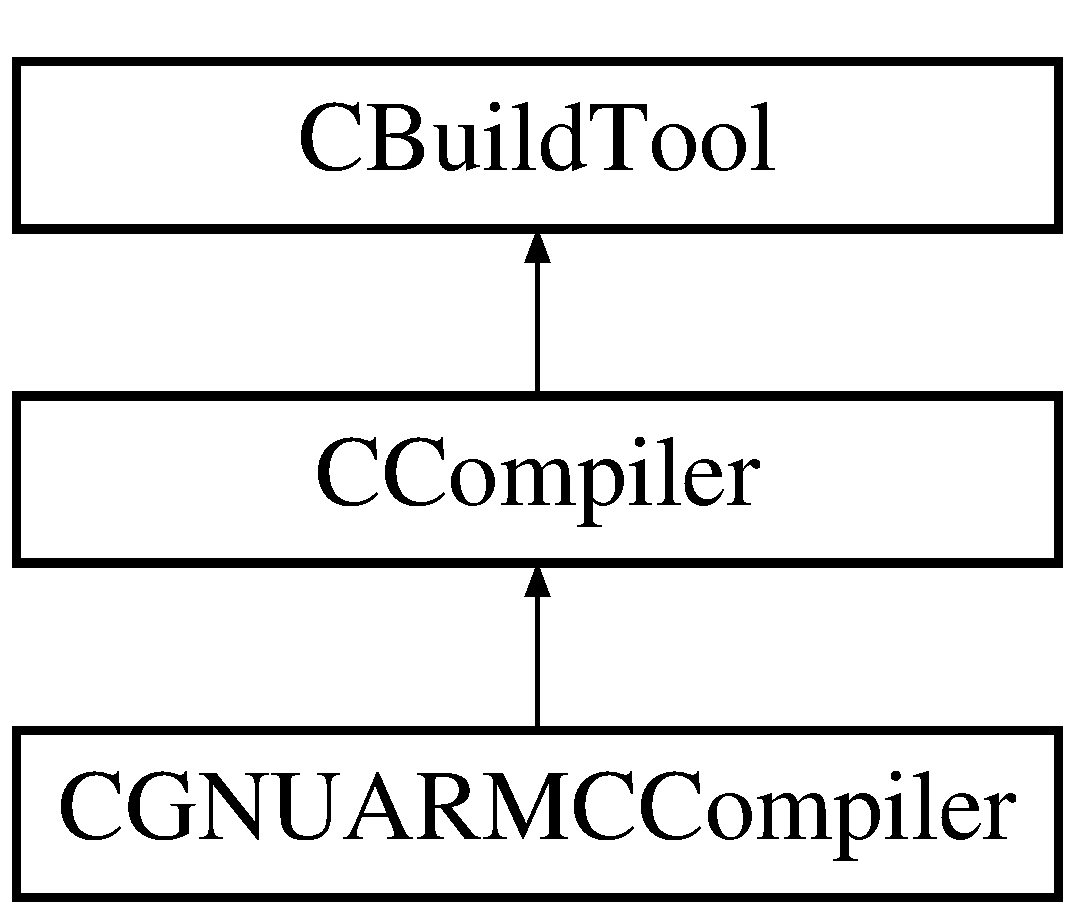
\includegraphics[height=3.000000cm]{d4/d7d/classCGNUARMCCompiler}
\end{center}
\end{figure}
\subsection*{Public Member Functions}
\begin{DoxyCompactItemize}
\item 
virtual \hyperlink{classCIncludeSearchFilter}{C\-Include\-Search\-Filter} $\ast$ \hyperlink{classCGNUARMCCompiler_a455c9c55a802d6a2e7e6d5146e252554}{Include\-Search\-Filter} (void) const 
\item 
virtual \hyperlink{classCGNUARMCCompiler}{C\-G\-N\-U\-A\-R\-M\-C\-Compiler} $\ast$ \hyperlink{classCGNUARMCCompiler_a3e102dcc65d172a098282c5554e79302}{Create\-Instance} (void)
\item 
virtual void \hyperlink{classCGNUARMCCompiler_a379674393ab735aae49e718d8da8d71a}{Reset} (const \hyperlink{classCPlatform_a2fb735c63c53052f79629e338bb0f535}{C\-Platform\-::\-O\-S\-\_\-\-Type} O\-S)
\item 
\hyperlink{classCGNUARMCCompiler_a7efc42cb3cc52d2dc0aac6e519b587bb}{C\-G\-N\-U\-A\-R\-M\-C\-Compiler} (void)
\end{DoxyCompactItemize}
\subsection*{Private Attributes}
\begin{DoxyCompactItemize}
\item 
\hyperlink{classCCppIncludeSearchFilter}{C\-Cpp\-Include\-Search\-Filter} \hyperlink{classCGNUARMCCompiler_abc5e6d8b8b6564fe7e8ba76c10be42ff}{m\-\_\-\-Include\-Search\-Filter}
\end{DoxyCompactItemize}
\subsection*{Additional Inherited Members}


\subsection{Constructor \& Destructor Documentation}
\hypertarget{classCGNUARMCCompiler_a7efc42cb3cc52d2dc0aac6e519b587bb}{\index{C\-G\-N\-U\-A\-R\-M\-C\-Compiler@{C\-G\-N\-U\-A\-R\-M\-C\-Compiler}!C\-G\-N\-U\-A\-R\-M\-C\-Compiler@{C\-G\-N\-U\-A\-R\-M\-C\-Compiler}}
\index{C\-G\-N\-U\-A\-R\-M\-C\-Compiler@{C\-G\-N\-U\-A\-R\-M\-C\-Compiler}!CGNUARMCCompiler@{C\-G\-N\-U\-A\-R\-M\-C\-Compiler}}
\subsubsection[{C\-G\-N\-U\-A\-R\-M\-C\-Compiler}]{\setlength{\rightskip}{0pt plus 5cm}C\-G\-N\-U\-A\-R\-M\-C\-Compiler\-::\-C\-G\-N\-U\-A\-R\-M\-C\-Compiler (
\begin{DoxyParamCaption}
\item[{void}]{}
\end{DoxyParamCaption}
)}}\label{classCGNUARMCCompiler_a7efc42cb3cc52d2dc0aac6e519b587bb}


\subsection{Member Function Documentation}
\hypertarget{classCGNUARMCCompiler_a3e102dcc65d172a098282c5554e79302}{\index{C\-G\-N\-U\-A\-R\-M\-C\-Compiler@{C\-G\-N\-U\-A\-R\-M\-C\-Compiler}!Create\-Instance@{Create\-Instance}}
\index{Create\-Instance@{Create\-Instance}!CGNUARMCCompiler@{C\-G\-N\-U\-A\-R\-M\-C\-Compiler}}
\subsubsection[{Create\-Instance}]{\setlength{\rightskip}{0pt plus 5cm}{\bf C\-G\-N\-U\-A\-R\-M\-C\-Compiler} $\ast$ C\-G\-N\-U\-A\-R\-M\-C\-Compiler\-::\-Create\-Instance (
\begin{DoxyParamCaption}
\item[{void}]{}
\end{DoxyParamCaption}
)\hspace{0.3cm}{\ttfamily [virtual]}}}\label{classCGNUARMCCompiler_a3e102dcc65d172a098282c5554e79302}


Reimplemented from \hyperlink{classCCompiler_a3d4aaaf69e1ba6070c729fd042d90012}{C\-Compiler}.

\hypertarget{classCGNUARMCCompiler_a455c9c55a802d6a2e7e6d5146e252554}{\index{C\-G\-N\-U\-A\-R\-M\-C\-Compiler@{C\-G\-N\-U\-A\-R\-M\-C\-Compiler}!Include\-Search\-Filter@{Include\-Search\-Filter}}
\index{Include\-Search\-Filter@{Include\-Search\-Filter}!CGNUARMCCompiler@{C\-G\-N\-U\-A\-R\-M\-C\-Compiler}}
\subsubsection[{Include\-Search\-Filter}]{\setlength{\rightskip}{0pt plus 5cm}{\bf C\-Include\-Search\-Filter} $\ast$ C\-G\-N\-U\-A\-R\-M\-C\-Compiler\-::\-Include\-Search\-Filter (
\begin{DoxyParamCaption}
\item[{void}]{}
\end{DoxyParamCaption}
) const\hspace{0.3cm}{\ttfamily [virtual]}}}\label{classCGNUARMCCompiler_a455c9c55a802d6a2e7e6d5146e252554}


Reimplemented from \hyperlink{classCCompiler_a1dc477f47e953ddd4c653f3ba85c5468}{C\-Compiler}.

\hypertarget{classCGNUARMCCompiler_a379674393ab735aae49e718d8da8d71a}{\index{C\-G\-N\-U\-A\-R\-M\-C\-Compiler@{C\-G\-N\-U\-A\-R\-M\-C\-Compiler}!Reset@{Reset}}
\index{Reset@{Reset}!CGNUARMCCompiler@{C\-G\-N\-U\-A\-R\-M\-C\-Compiler}}
\subsubsection[{Reset}]{\setlength{\rightskip}{0pt plus 5cm}void C\-G\-N\-U\-A\-R\-M\-C\-Compiler\-::\-Reset (
\begin{DoxyParamCaption}
\item[{const {\bf C\-Platform\-::\-O\-S\-\_\-\-Type}}]{O\-S}
\end{DoxyParamCaption}
)\hspace{0.3cm}{\ttfamily [virtual]}}}\label{classCGNUARMCCompiler_a379674393ab735aae49e718d8da8d71a}


Reimplemented from \hyperlink{classCBuildTool_abea21a0e61ab2177effdff5aaa169585}{C\-Build\-Tool}.



\subsection{Member Data Documentation}
\hypertarget{classCGNUARMCCompiler_abc5e6d8b8b6564fe7e8ba76c10be42ff}{\index{C\-G\-N\-U\-A\-R\-M\-C\-Compiler@{C\-G\-N\-U\-A\-R\-M\-C\-Compiler}!m\-\_\-\-Include\-Search\-Filter@{m\-\_\-\-Include\-Search\-Filter}}
\index{m\-\_\-\-Include\-Search\-Filter@{m\-\_\-\-Include\-Search\-Filter}!CGNUARMCCompiler@{C\-G\-N\-U\-A\-R\-M\-C\-Compiler}}
\subsubsection[{m\-\_\-\-Include\-Search\-Filter}]{\setlength{\rightskip}{0pt plus 5cm}{\bf C\-Cpp\-Include\-Search\-Filter} C\-G\-N\-U\-A\-R\-M\-C\-Compiler\-::m\-\_\-\-Include\-Search\-Filter\hspace{0.3cm}{\ttfamily [private]}}}\label{classCGNUARMCCompiler_abc5e6d8b8b6564fe7e8ba76c10be42ff}


The documentation for this class was generated from the following files\-:\begin{DoxyCompactItemize}
\item 
src/\hyperlink{buildtools_8h}{buildtools.\-h}\item 
src/\hyperlink{buildtools_8cpp}{buildtools.\-cpp}\end{DoxyCompactItemize}

\hypertarget{classCGNUARMCppCompiler}{\section{C\-G\-N\-U\-A\-R\-M\-Cpp\-Compiler Class Reference}
\label{classCGNUARMCppCompiler}\index{C\-G\-N\-U\-A\-R\-M\-Cpp\-Compiler@{C\-G\-N\-U\-A\-R\-M\-Cpp\-Compiler}}
}


{\ttfamily \#include $<$buildtools.\-h$>$}

Inheritance diagram for C\-G\-N\-U\-A\-R\-M\-Cpp\-Compiler\-:\begin{figure}[H]
\begin{center}
\leavevmode
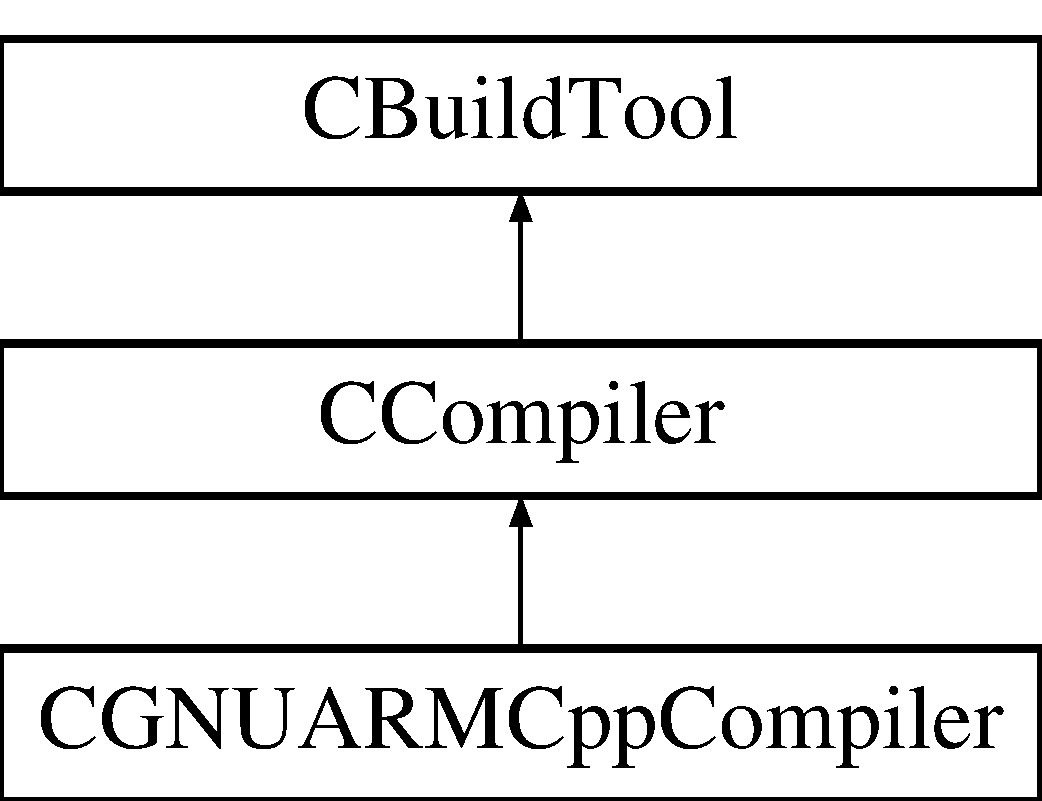
\includegraphics[height=3.000000cm]{d0/d77/classCGNUARMCppCompiler}
\end{center}
\end{figure}
\subsection*{Public Member Functions}
\begin{DoxyCompactItemize}
\item 
virtual \hyperlink{classCIncludeSearchFilter}{C\-Include\-Search\-Filter} $\ast$ \hyperlink{classCGNUARMCppCompiler_a061d65ad921d3856be6e2b8f80976106}{Include\-Search\-Filter} (void) const 
\item 
virtual \hyperlink{classCGNUARMCppCompiler}{C\-G\-N\-U\-A\-R\-M\-Cpp\-Compiler} $\ast$ \hyperlink{classCGNUARMCppCompiler_ae61a4db30f31a36bc46341da83ac9c63}{Create\-Instance} (void)
\item 
virtual void \hyperlink{classCGNUARMCppCompiler_aa51e81dcb2d4a6982aae3c8627e3fdc6}{Reset} (const \hyperlink{classCPlatform_a2fb735c63c53052f79629e338bb0f535}{C\-Platform\-::\-O\-S\-\_\-\-Type} O\-S)
\item 
\hyperlink{classCGNUARMCppCompiler_a7b41dd8037c30c9be8f0797c3180cb0f}{C\-G\-N\-U\-A\-R\-M\-Cpp\-Compiler} (void)
\end{DoxyCompactItemize}
\subsection*{Private Attributes}
\begin{DoxyCompactItemize}
\item 
\hyperlink{classCCppIncludeSearchFilter}{C\-Cpp\-Include\-Search\-Filter} \hyperlink{classCGNUARMCppCompiler_a18c1f490cdec9e19133ae5782554b073}{m\-\_\-\-Include\-Search\-Filter}
\end{DoxyCompactItemize}
\subsection*{Additional Inherited Members}


\subsection{Constructor \& Destructor Documentation}
\hypertarget{classCGNUARMCppCompiler_a7b41dd8037c30c9be8f0797c3180cb0f}{\index{C\-G\-N\-U\-A\-R\-M\-Cpp\-Compiler@{C\-G\-N\-U\-A\-R\-M\-Cpp\-Compiler}!C\-G\-N\-U\-A\-R\-M\-Cpp\-Compiler@{C\-G\-N\-U\-A\-R\-M\-Cpp\-Compiler}}
\index{C\-G\-N\-U\-A\-R\-M\-Cpp\-Compiler@{C\-G\-N\-U\-A\-R\-M\-Cpp\-Compiler}!CGNUARMCppCompiler@{C\-G\-N\-U\-A\-R\-M\-Cpp\-Compiler}}
\subsubsection[{C\-G\-N\-U\-A\-R\-M\-Cpp\-Compiler}]{\setlength{\rightskip}{0pt plus 5cm}C\-G\-N\-U\-A\-R\-M\-Cpp\-Compiler\-::\-C\-G\-N\-U\-A\-R\-M\-Cpp\-Compiler (
\begin{DoxyParamCaption}
\item[{void}]{}
\end{DoxyParamCaption}
)}}\label{classCGNUARMCppCompiler_a7b41dd8037c30c9be8f0797c3180cb0f}


\subsection{Member Function Documentation}
\hypertarget{classCGNUARMCppCompiler_ae61a4db30f31a36bc46341da83ac9c63}{\index{C\-G\-N\-U\-A\-R\-M\-Cpp\-Compiler@{C\-G\-N\-U\-A\-R\-M\-Cpp\-Compiler}!Create\-Instance@{Create\-Instance}}
\index{Create\-Instance@{Create\-Instance}!CGNUARMCppCompiler@{C\-G\-N\-U\-A\-R\-M\-Cpp\-Compiler}}
\subsubsection[{Create\-Instance}]{\setlength{\rightskip}{0pt plus 5cm}{\bf C\-G\-N\-U\-A\-R\-M\-Cpp\-Compiler} $\ast$ C\-G\-N\-U\-A\-R\-M\-Cpp\-Compiler\-::\-Create\-Instance (
\begin{DoxyParamCaption}
\item[{void}]{}
\end{DoxyParamCaption}
)\hspace{0.3cm}{\ttfamily [virtual]}}}\label{classCGNUARMCppCompiler_ae61a4db30f31a36bc46341da83ac9c63}


Reimplemented from \hyperlink{classCCompiler_a3d4aaaf69e1ba6070c729fd042d90012}{C\-Compiler}.

\hypertarget{classCGNUARMCppCompiler_a061d65ad921d3856be6e2b8f80976106}{\index{C\-G\-N\-U\-A\-R\-M\-Cpp\-Compiler@{C\-G\-N\-U\-A\-R\-M\-Cpp\-Compiler}!Include\-Search\-Filter@{Include\-Search\-Filter}}
\index{Include\-Search\-Filter@{Include\-Search\-Filter}!CGNUARMCppCompiler@{C\-G\-N\-U\-A\-R\-M\-Cpp\-Compiler}}
\subsubsection[{Include\-Search\-Filter}]{\setlength{\rightskip}{0pt plus 5cm}{\bf C\-Include\-Search\-Filter} $\ast$ C\-G\-N\-U\-A\-R\-M\-Cpp\-Compiler\-::\-Include\-Search\-Filter (
\begin{DoxyParamCaption}
\item[{void}]{}
\end{DoxyParamCaption}
) const\hspace{0.3cm}{\ttfamily [virtual]}}}\label{classCGNUARMCppCompiler_a061d65ad921d3856be6e2b8f80976106}


Reimplemented from \hyperlink{classCCompiler_a1dc477f47e953ddd4c653f3ba85c5468}{C\-Compiler}.

\hypertarget{classCGNUARMCppCompiler_aa51e81dcb2d4a6982aae3c8627e3fdc6}{\index{C\-G\-N\-U\-A\-R\-M\-Cpp\-Compiler@{C\-G\-N\-U\-A\-R\-M\-Cpp\-Compiler}!Reset@{Reset}}
\index{Reset@{Reset}!CGNUARMCppCompiler@{C\-G\-N\-U\-A\-R\-M\-Cpp\-Compiler}}
\subsubsection[{Reset}]{\setlength{\rightskip}{0pt plus 5cm}void C\-G\-N\-U\-A\-R\-M\-Cpp\-Compiler\-::\-Reset (
\begin{DoxyParamCaption}
\item[{const {\bf C\-Platform\-::\-O\-S\-\_\-\-Type}}]{O\-S}
\end{DoxyParamCaption}
)\hspace{0.3cm}{\ttfamily [virtual]}}}\label{classCGNUARMCppCompiler_aa51e81dcb2d4a6982aae3c8627e3fdc6}


Reimplemented from \hyperlink{classCBuildTool_abea21a0e61ab2177effdff5aaa169585}{C\-Build\-Tool}.



\subsection{Member Data Documentation}
\hypertarget{classCGNUARMCppCompiler_a18c1f490cdec9e19133ae5782554b073}{\index{C\-G\-N\-U\-A\-R\-M\-Cpp\-Compiler@{C\-G\-N\-U\-A\-R\-M\-Cpp\-Compiler}!m\-\_\-\-Include\-Search\-Filter@{m\-\_\-\-Include\-Search\-Filter}}
\index{m\-\_\-\-Include\-Search\-Filter@{m\-\_\-\-Include\-Search\-Filter}!CGNUARMCppCompiler@{C\-G\-N\-U\-A\-R\-M\-Cpp\-Compiler}}
\subsubsection[{m\-\_\-\-Include\-Search\-Filter}]{\setlength{\rightskip}{0pt plus 5cm}{\bf C\-Cpp\-Include\-Search\-Filter} C\-G\-N\-U\-A\-R\-M\-Cpp\-Compiler\-::m\-\_\-\-Include\-Search\-Filter\hspace{0.3cm}{\ttfamily [private]}}}\label{classCGNUARMCppCompiler_a18c1f490cdec9e19133ae5782554b073}


The documentation for this class was generated from the following files\-:\begin{DoxyCompactItemize}
\item 
src/\hyperlink{buildtools_8h}{buildtools.\-h}\item 
src/\hyperlink{buildtools_8cpp}{buildtools.\-cpp}\end{DoxyCompactItemize}

\hypertarget{classCGNUARMDynamicLinker}{\section{C\-G\-N\-U\-A\-R\-M\-Dynamic\-Linker Class Reference}
\label{classCGNUARMDynamicLinker}\index{C\-G\-N\-U\-A\-R\-M\-Dynamic\-Linker@{C\-G\-N\-U\-A\-R\-M\-Dynamic\-Linker}}
}


{\ttfamily \#include $<$buildtools.\-h$>$}

Inheritance diagram for C\-G\-N\-U\-A\-R\-M\-Dynamic\-Linker\-:\begin{figure}[H]
\begin{center}
\leavevmode
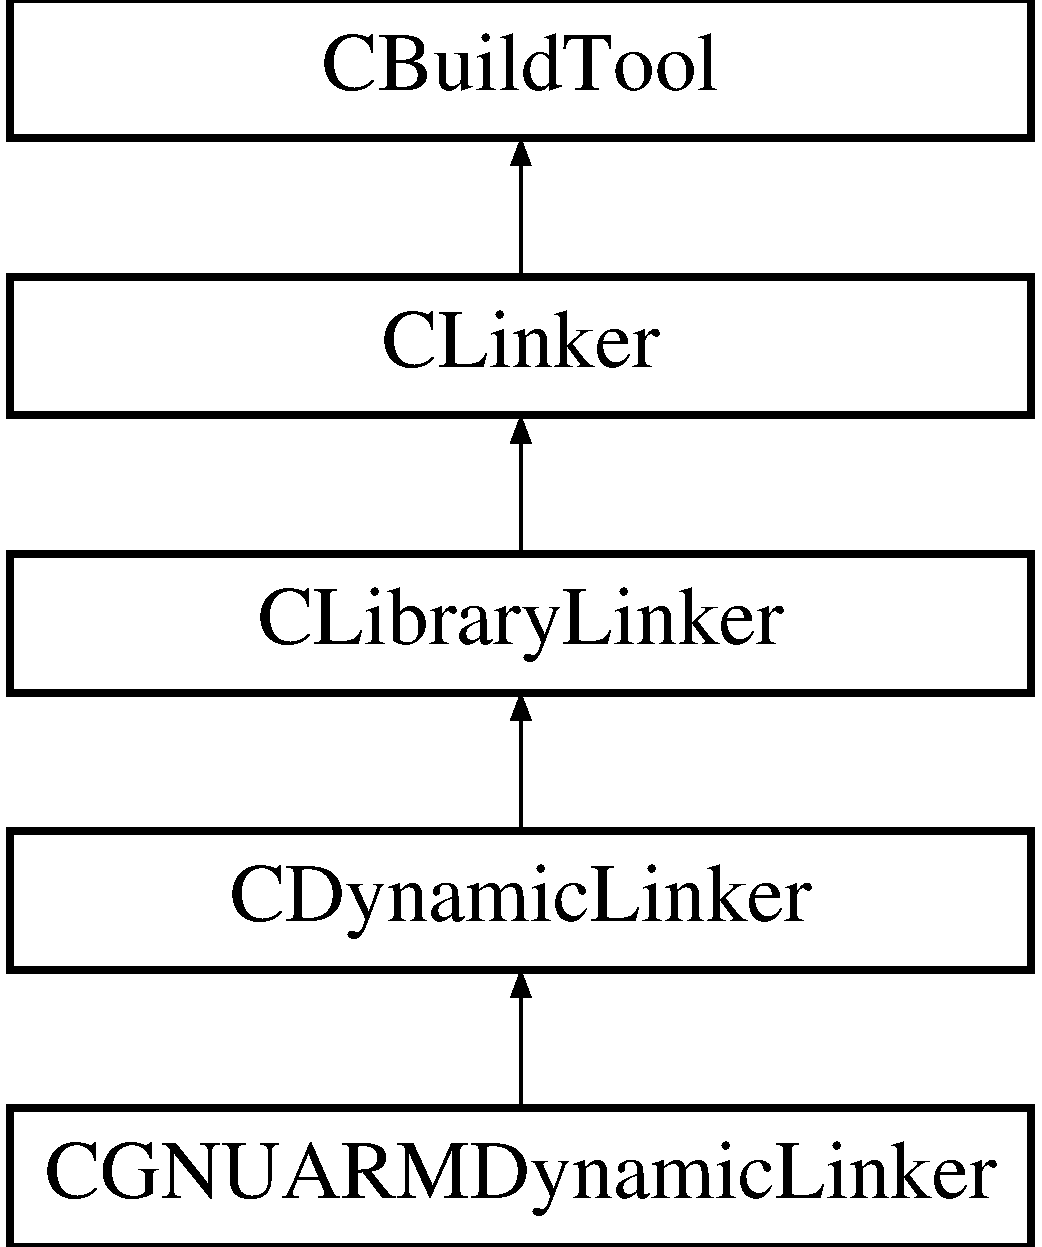
\includegraphics[height=5.000000cm]{de/d4d/classCGNUARMDynamicLinker}
\end{center}
\end{figure}
\subsection*{Public Member Functions}
\begin{DoxyCompactItemize}
\item 
virtual \hyperlink{classCGNUARMDynamicLinker}{C\-G\-N\-U\-A\-R\-M\-Dynamic\-Linker} $\ast$ \hyperlink{classCGNUARMDynamicLinker_ad3ded52b8101b6f85ad6d5609f85c78c}{Create\-Instance} (void)
\item 
virtual void \hyperlink{classCGNUARMDynamicLinker_a3f49a2938f97c58d9eaee0986f3b9866}{Reset} (const \hyperlink{classCPlatform_a2fb735c63c53052f79629e338bb0f535}{C\-Platform\-::\-O\-S\-\_\-\-Type} O\-S)
\item 
\hyperlink{classCGNUARMDynamicLinker_a1498e3b3b35f22a205c77e9012205d69}{C\-G\-N\-U\-A\-R\-M\-Dynamic\-Linker} (void)
\end{DoxyCompactItemize}
\subsection*{Additional Inherited Members}


\subsection{Constructor \& Destructor Documentation}
\hypertarget{classCGNUARMDynamicLinker_a1498e3b3b35f22a205c77e9012205d69}{\index{C\-G\-N\-U\-A\-R\-M\-Dynamic\-Linker@{C\-G\-N\-U\-A\-R\-M\-Dynamic\-Linker}!C\-G\-N\-U\-A\-R\-M\-Dynamic\-Linker@{C\-G\-N\-U\-A\-R\-M\-Dynamic\-Linker}}
\index{C\-G\-N\-U\-A\-R\-M\-Dynamic\-Linker@{C\-G\-N\-U\-A\-R\-M\-Dynamic\-Linker}!CGNUARMDynamicLinker@{C\-G\-N\-U\-A\-R\-M\-Dynamic\-Linker}}
\subsubsection[{C\-G\-N\-U\-A\-R\-M\-Dynamic\-Linker}]{\setlength{\rightskip}{0pt plus 5cm}C\-G\-N\-U\-A\-R\-M\-Dynamic\-Linker\-::\-C\-G\-N\-U\-A\-R\-M\-Dynamic\-Linker (
\begin{DoxyParamCaption}
\item[{void}]{}
\end{DoxyParamCaption}
)}}\label{classCGNUARMDynamicLinker_a1498e3b3b35f22a205c77e9012205d69}


\subsection{Member Function Documentation}
\hypertarget{classCGNUARMDynamicLinker_ad3ded52b8101b6f85ad6d5609f85c78c}{\index{C\-G\-N\-U\-A\-R\-M\-Dynamic\-Linker@{C\-G\-N\-U\-A\-R\-M\-Dynamic\-Linker}!Create\-Instance@{Create\-Instance}}
\index{Create\-Instance@{Create\-Instance}!CGNUARMDynamicLinker@{C\-G\-N\-U\-A\-R\-M\-Dynamic\-Linker}}
\subsubsection[{Create\-Instance}]{\setlength{\rightskip}{0pt plus 5cm}{\bf C\-G\-N\-U\-A\-R\-M\-Dynamic\-Linker} $\ast$ C\-G\-N\-U\-A\-R\-M\-Dynamic\-Linker\-::\-Create\-Instance (
\begin{DoxyParamCaption}
\item[{void}]{}
\end{DoxyParamCaption}
)\hspace{0.3cm}{\ttfamily [virtual]}}}\label{classCGNUARMDynamicLinker_ad3ded52b8101b6f85ad6d5609f85c78c}


Reimplemented from \hyperlink{classCDynamicLinker_ac71406ca5c6e8e991a6418a6307d274c}{C\-Dynamic\-Linker}.

\hypertarget{classCGNUARMDynamicLinker_a3f49a2938f97c58d9eaee0986f3b9866}{\index{C\-G\-N\-U\-A\-R\-M\-Dynamic\-Linker@{C\-G\-N\-U\-A\-R\-M\-Dynamic\-Linker}!Reset@{Reset}}
\index{Reset@{Reset}!CGNUARMDynamicLinker@{C\-G\-N\-U\-A\-R\-M\-Dynamic\-Linker}}
\subsubsection[{Reset}]{\setlength{\rightskip}{0pt plus 5cm}void C\-G\-N\-U\-A\-R\-M\-Dynamic\-Linker\-::\-Reset (
\begin{DoxyParamCaption}
\item[{const {\bf C\-Platform\-::\-O\-S\-\_\-\-Type}}]{O\-S}
\end{DoxyParamCaption}
)\hspace{0.3cm}{\ttfamily [virtual]}}}\label{classCGNUARMDynamicLinker_a3f49a2938f97c58d9eaee0986f3b9866}


Reimplemented from \hyperlink{classCDynamicLinker_a437d46ee65b3585e7be9d15d40c26820}{C\-Dynamic\-Linker}.



The documentation for this class was generated from the following files\-:\begin{DoxyCompactItemize}
\item 
src/\hyperlink{buildtools_8h}{buildtools.\-h}\item 
src/\hyperlink{buildtools_8cpp}{buildtools.\-cpp}\end{DoxyCompactItemize}

\hypertarget{classCGNUARMExecutableLinker}{\section{C\-G\-N\-U\-A\-R\-M\-Executable\-Linker Class Reference}
\label{classCGNUARMExecutableLinker}\index{C\-G\-N\-U\-A\-R\-M\-Executable\-Linker@{C\-G\-N\-U\-A\-R\-M\-Executable\-Linker}}
}


{\ttfamily \#include $<$buildtools.\-h$>$}

Inheritance diagram for C\-G\-N\-U\-A\-R\-M\-Executable\-Linker\-:\begin{figure}[H]
\begin{center}
\leavevmode
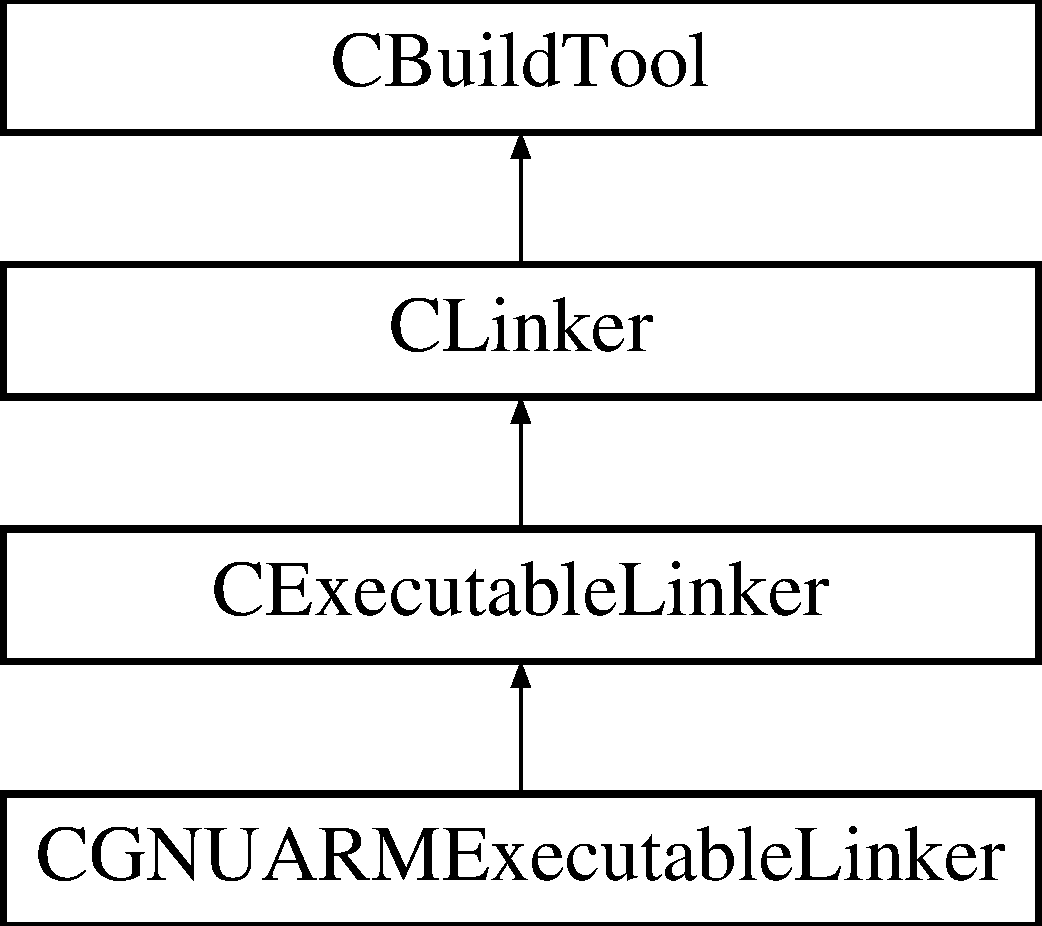
\includegraphics[height=4.000000cm]{d2/dfe/classCGNUARMExecutableLinker}
\end{center}
\end{figure}
\subsection*{Public Member Functions}
\begin{DoxyCompactItemize}
\item 
virtual \hyperlink{classCGNUARMExecutableLinker}{C\-G\-N\-U\-A\-R\-M\-Executable\-Linker} $\ast$ \hyperlink{classCGNUARMExecutableLinker_a9241ead8113a3c4c3820240f3993fb19}{Create\-Instance} (void)
\item 
virtual void \hyperlink{classCGNUARMExecutableLinker_a9c3143f13605d317022dca24f134ff39}{Reset} (const \hyperlink{classCPlatform_a2fb735c63c53052f79629e338bb0f535}{C\-Platform\-::\-O\-S\-\_\-\-Type} O\-S)
\item 
\hyperlink{classCGNUARMExecutableLinker_a80b88af8b1d8360070e9b32dd236c955}{C\-G\-N\-U\-A\-R\-M\-Executable\-Linker} (void)
\end{DoxyCompactItemize}
\subsection*{Additional Inherited Members}


\subsection{Constructor \& Destructor Documentation}
\hypertarget{classCGNUARMExecutableLinker_a80b88af8b1d8360070e9b32dd236c955}{\index{C\-G\-N\-U\-A\-R\-M\-Executable\-Linker@{C\-G\-N\-U\-A\-R\-M\-Executable\-Linker}!C\-G\-N\-U\-A\-R\-M\-Executable\-Linker@{C\-G\-N\-U\-A\-R\-M\-Executable\-Linker}}
\index{C\-G\-N\-U\-A\-R\-M\-Executable\-Linker@{C\-G\-N\-U\-A\-R\-M\-Executable\-Linker}!CGNUARMExecutableLinker@{C\-G\-N\-U\-A\-R\-M\-Executable\-Linker}}
\subsubsection[{C\-G\-N\-U\-A\-R\-M\-Executable\-Linker}]{\setlength{\rightskip}{0pt plus 5cm}C\-G\-N\-U\-A\-R\-M\-Executable\-Linker\-::\-C\-G\-N\-U\-A\-R\-M\-Executable\-Linker (
\begin{DoxyParamCaption}
\item[{void}]{}
\end{DoxyParamCaption}
)}}\label{classCGNUARMExecutableLinker_a80b88af8b1d8360070e9b32dd236c955}


\subsection{Member Function Documentation}
\hypertarget{classCGNUARMExecutableLinker_a9241ead8113a3c4c3820240f3993fb19}{\index{C\-G\-N\-U\-A\-R\-M\-Executable\-Linker@{C\-G\-N\-U\-A\-R\-M\-Executable\-Linker}!Create\-Instance@{Create\-Instance}}
\index{Create\-Instance@{Create\-Instance}!CGNUARMExecutableLinker@{C\-G\-N\-U\-A\-R\-M\-Executable\-Linker}}
\subsubsection[{Create\-Instance}]{\setlength{\rightskip}{0pt plus 5cm}{\bf C\-G\-N\-U\-A\-R\-M\-Executable\-Linker} $\ast$ C\-G\-N\-U\-A\-R\-M\-Executable\-Linker\-::\-Create\-Instance (
\begin{DoxyParamCaption}
\item[{void}]{}
\end{DoxyParamCaption}
)\hspace{0.3cm}{\ttfamily [virtual]}}}\label{classCGNUARMExecutableLinker_a9241ead8113a3c4c3820240f3993fb19}


Reimplemented from \hyperlink{classCExecutableLinker_a457b823b737b0a78285d5ede77df827c}{C\-Executable\-Linker}.

\hypertarget{classCGNUARMExecutableLinker_a9c3143f13605d317022dca24f134ff39}{\index{C\-G\-N\-U\-A\-R\-M\-Executable\-Linker@{C\-G\-N\-U\-A\-R\-M\-Executable\-Linker}!Reset@{Reset}}
\index{Reset@{Reset}!CGNUARMExecutableLinker@{C\-G\-N\-U\-A\-R\-M\-Executable\-Linker}}
\subsubsection[{Reset}]{\setlength{\rightskip}{0pt plus 5cm}void C\-G\-N\-U\-A\-R\-M\-Executable\-Linker\-::\-Reset (
\begin{DoxyParamCaption}
\item[{const {\bf C\-Platform\-::\-O\-S\-\_\-\-Type}}]{O\-S}
\end{DoxyParamCaption}
)\hspace{0.3cm}{\ttfamily [virtual]}}}\label{classCGNUARMExecutableLinker_a9c3143f13605d317022dca24f134ff39}


Reimplemented from \hyperlink{classCBuildTool_abea21a0e61ab2177effdff5aaa169585}{C\-Build\-Tool}.



The documentation for this class was generated from the following files\-:\begin{DoxyCompactItemize}
\item 
src/\hyperlink{buildtools_8h}{buildtools.\-h}\item 
src/\hyperlink{buildtools_8cpp}{buildtools.\-cpp}\end{DoxyCompactItemize}

\hypertarget{classCGNUARMStaticLinker}{\section{C\-G\-N\-U\-A\-R\-M\-Static\-Linker Class Reference}
\label{classCGNUARMStaticLinker}\index{C\-G\-N\-U\-A\-R\-M\-Static\-Linker@{C\-G\-N\-U\-A\-R\-M\-Static\-Linker}}
}


{\ttfamily \#include $<$buildtools.\-h$>$}

Inheritance diagram for C\-G\-N\-U\-A\-R\-M\-Static\-Linker\-:\begin{figure}[H]
\begin{center}
\leavevmode
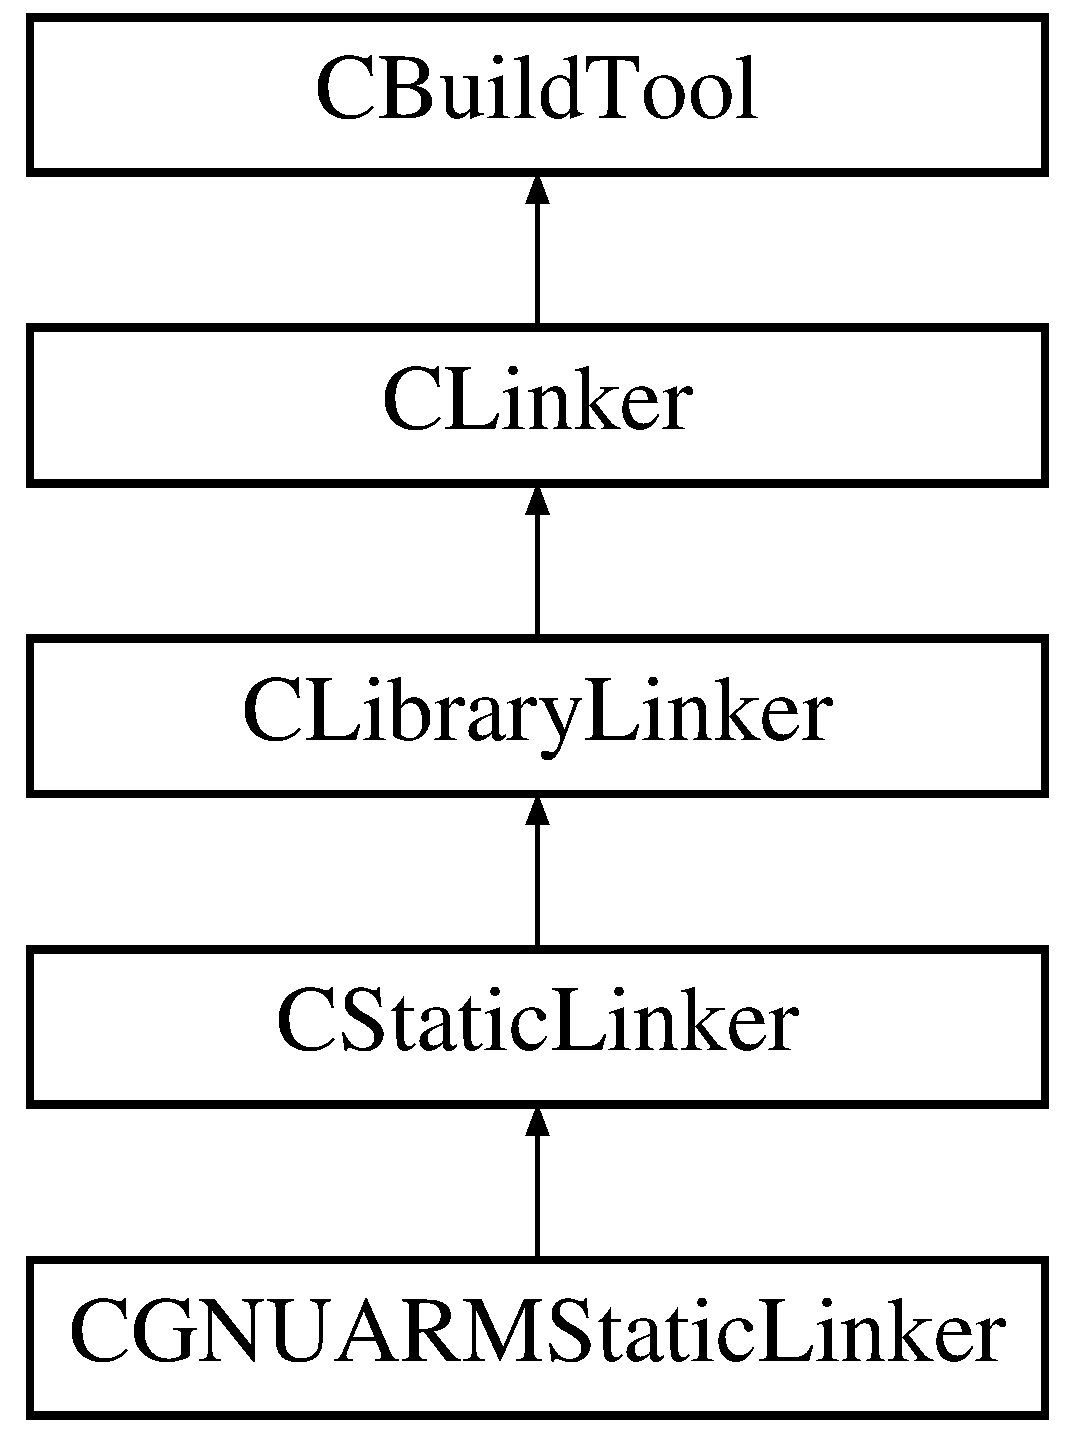
\includegraphics[height=5.000000cm]{d8/d07/classCGNUARMStaticLinker}
\end{center}
\end{figure}
\subsection*{Public Member Functions}
\begin{DoxyCompactItemize}
\item 
virtual \hyperlink{classCGNUARMStaticLinker}{C\-G\-N\-U\-A\-R\-M\-Static\-Linker} $\ast$ \hyperlink{classCGNUARMStaticLinker_a7cac8fed64437b826d085b0cf33aeaf8}{Create\-Instance} (void)
\item 
virtual void \hyperlink{classCGNUARMStaticLinker_a2bb9852d9ddd5ad71fdd2bb9a374343e}{Reset} (const \hyperlink{classCPlatform_a2fb735c63c53052f79629e338bb0f535}{C\-Platform\-::\-O\-S\-\_\-\-Type} O\-S)
\item 
\hyperlink{classCGNUARMStaticLinker_a3f8cc2178206f0be0de268d862974efe}{C\-G\-N\-U\-A\-R\-M\-Static\-Linker} (void)
\end{DoxyCompactItemize}
\subsection*{Additional Inherited Members}


\subsection{Constructor \& Destructor Documentation}
\hypertarget{classCGNUARMStaticLinker_a3f8cc2178206f0be0de268d862974efe}{\index{C\-G\-N\-U\-A\-R\-M\-Static\-Linker@{C\-G\-N\-U\-A\-R\-M\-Static\-Linker}!C\-G\-N\-U\-A\-R\-M\-Static\-Linker@{C\-G\-N\-U\-A\-R\-M\-Static\-Linker}}
\index{C\-G\-N\-U\-A\-R\-M\-Static\-Linker@{C\-G\-N\-U\-A\-R\-M\-Static\-Linker}!CGNUARMStaticLinker@{C\-G\-N\-U\-A\-R\-M\-Static\-Linker}}
\subsubsection[{C\-G\-N\-U\-A\-R\-M\-Static\-Linker}]{\setlength{\rightskip}{0pt plus 5cm}C\-G\-N\-U\-A\-R\-M\-Static\-Linker\-::\-C\-G\-N\-U\-A\-R\-M\-Static\-Linker (
\begin{DoxyParamCaption}
\item[{void}]{}
\end{DoxyParamCaption}
)}}\label{classCGNUARMStaticLinker_a3f8cc2178206f0be0de268d862974efe}


\subsection{Member Function Documentation}
\hypertarget{classCGNUARMStaticLinker_a7cac8fed64437b826d085b0cf33aeaf8}{\index{C\-G\-N\-U\-A\-R\-M\-Static\-Linker@{C\-G\-N\-U\-A\-R\-M\-Static\-Linker}!Create\-Instance@{Create\-Instance}}
\index{Create\-Instance@{Create\-Instance}!CGNUARMStaticLinker@{C\-G\-N\-U\-A\-R\-M\-Static\-Linker}}
\subsubsection[{Create\-Instance}]{\setlength{\rightskip}{0pt plus 5cm}{\bf C\-G\-N\-U\-A\-R\-M\-Static\-Linker} $\ast$ C\-G\-N\-U\-A\-R\-M\-Static\-Linker\-::\-Create\-Instance (
\begin{DoxyParamCaption}
\item[{void}]{}
\end{DoxyParamCaption}
)\hspace{0.3cm}{\ttfamily [virtual]}}}\label{classCGNUARMStaticLinker_a7cac8fed64437b826d085b0cf33aeaf8}


Reimplemented from \hyperlink{classCStaticLinker_a7e626491caa847ef207032ee600625db}{C\-Static\-Linker}.

\hypertarget{classCGNUARMStaticLinker_a2bb9852d9ddd5ad71fdd2bb9a374343e}{\index{C\-G\-N\-U\-A\-R\-M\-Static\-Linker@{C\-G\-N\-U\-A\-R\-M\-Static\-Linker}!Reset@{Reset}}
\index{Reset@{Reset}!CGNUARMStaticLinker@{C\-G\-N\-U\-A\-R\-M\-Static\-Linker}}
\subsubsection[{Reset}]{\setlength{\rightskip}{0pt plus 5cm}void C\-G\-N\-U\-A\-R\-M\-Static\-Linker\-::\-Reset (
\begin{DoxyParamCaption}
\item[{const {\bf C\-Platform\-::\-O\-S\-\_\-\-Type}}]{O\-S}
\end{DoxyParamCaption}
)\hspace{0.3cm}{\ttfamily [virtual]}}}\label{classCGNUARMStaticLinker_a2bb9852d9ddd5ad71fdd2bb9a374343e}


Reimplemented from \hyperlink{classCBuildTool_abea21a0e61ab2177effdff5aaa169585}{C\-Build\-Tool}.



The documentation for this class was generated from the following files\-:\begin{DoxyCompactItemize}
\item 
src/\hyperlink{buildtools_8h}{buildtools.\-h}\item 
src/\hyperlink{buildtools_8cpp}{buildtools.\-cpp}\end{DoxyCompactItemize}

\hypertarget{classCGNUARMWindowsResourceCompiler}{\section{C\-G\-N\-U\-A\-R\-M\-Windows\-Resource\-Compiler Class Reference}
\label{classCGNUARMWindowsResourceCompiler}\index{C\-G\-N\-U\-A\-R\-M\-Windows\-Resource\-Compiler@{C\-G\-N\-U\-A\-R\-M\-Windows\-Resource\-Compiler}}
}


{\ttfamily \#include $<$buildtools.\-h$>$}

Inheritance diagram for C\-G\-N\-U\-A\-R\-M\-Windows\-Resource\-Compiler\-:\begin{figure}[H]
\begin{center}
\leavevmode
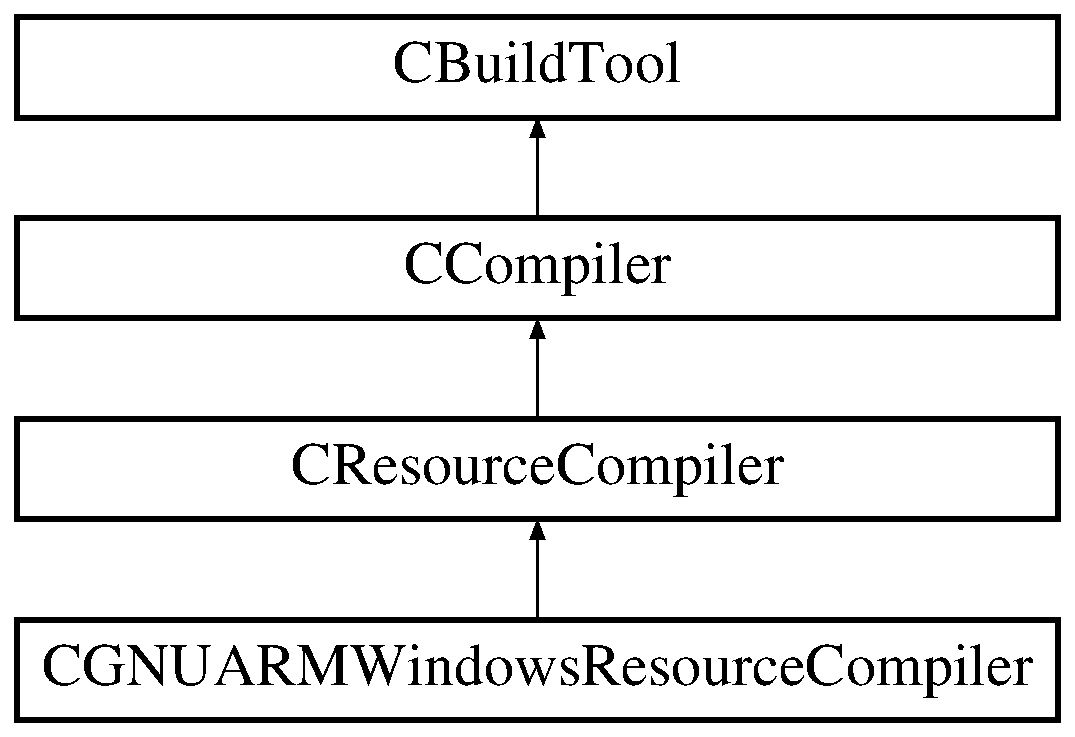
\includegraphics[height=4.000000cm]{d6/d48/classCGNUARMWindowsResourceCompiler}
\end{center}
\end{figure}
\subsection*{Public Member Functions}
\begin{DoxyCompactItemize}
\item 
virtual \\*
\hyperlink{classCGNUARMWindowsResourceCompiler}{C\-G\-N\-U\-A\-R\-M\-Windows\-Resource\-Compiler} $\ast$ \hyperlink{classCGNUARMWindowsResourceCompiler_a8da0eff0b561e69f2e2178965cd69253}{Create\-Instance} (void)
\item 
virtual void \hyperlink{classCGNUARMWindowsResourceCompiler_a0eae18d396f5bfc5ffcd76af42b8d093}{Reset} (const \hyperlink{classCPlatform_a2fb735c63c53052f79629e338bb0f535}{C\-Platform\-::\-O\-S\-\_\-\-Type} O\-S)
\item 
virtual bool \hyperlink{classCGNUARMWindowsResourceCompiler_abffeeed1b3f8b6482c231c7349098f0c}{Supports} (const \hyperlink{classCPlatform_a2fb735c63c53052f79629e338bb0f535}{C\-Platform\-::\-O\-S\-\_\-\-Type} O\-S)
\item 
\hyperlink{classCGNUARMWindowsResourceCompiler_aacc47687b1ea60b470580cfa7de868e2}{C\-G\-N\-U\-A\-R\-M\-Windows\-Resource\-Compiler} (void)
\end{DoxyCompactItemize}
\subsection*{Additional Inherited Members}


\subsection{Constructor \& Destructor Documentation}
\hypertarget{classCGNUARMWindowsResourceCompiler_aacc47687b1ea60b470580cfa7de868e2}{\index{C\-G\-N\-U\-A\-R\-M\-Windows\-Resource\-Compiler@{C\-G\-N\-U\-A\-R\-M\-Windows\-Resource\-Compiler}!C\-G\-N\-U\-A\-R\-M\-Windows\-Resource\-Compiler@{C\-G\-N\-U\-A\-R\-M\-Windows\-Resource\-Compiler}}
\index{C\-G\-N\-U\-A\-R\-M\-Windows\-Resource\-Compiler@{C\-G\-N\-U\-A\-R\-M\-Windows\-Resource\-Compiler}!CGNUARMWindowsResourceCompiler@{C\-G\-N\-U\-A\-R\-M\-Windows\-Resource\-Compiler}}
\subsubsection[{C\-G\-N\-U\-A\-R\-M\-Windows\-Resource\-Compiler}]{\setlength{\rightskip}{0pt plus 5cm}C\-G\-N\-U\-A\-R\-M\-Windows\-Resource\-Compiler\-::\-C\-G\-N\-U\-A\-R\-M\-Windows\-Resource\-Compiler (
\begin{DoxyParamCaption}
\item[{void}]{}
\end{DoxyParamCaption}
)}}\label{classCGNUARMWindowsResourceCompiler_aacc47687b1ea60b470580cfa7de868e2}


\subsection{Member Function Documentation}
\hypertarget{classCGNUARMWindowsResourceCompiler_a8da0eff0b561e69f2e2178965cd69253}{\index{C\-G\-N\-U\-A\-R\-M\-Windows\-Resource\-Compiler@{C\-G\-N\-U\-A\-R\-M\-Windows\-Resource\-Compiler}!Create\-Instance@{Create\-Instance}}
\index{Create\-Instance@{Create\-Instance}!CGNUARMWindowsResourceCompiler@{C\-G\-N\-U\-A\-R\-M\-Windows\-Resource\-Compiler}}
\subsubsection[{Create\-Instance}]{\setlength{\rightskip}{0pt plus 5cm}virtual {\bf C\-G\-N\-U\-A\-R\-M\-Windows\-Resource\-Compiler}$\ast$ C\-G\-N\-U\-A\-R\-M\-Windows\-Resource\-Compiler\-::\-Create\-Instance (
\begin{DoxyParamCaption}
\item[{void}]{}
\end{DoxyParamCaption}
)\hspace{0.3cm}{\ttfamily [virtual]}}}\label{classCGNUARMWindowsResourceCompiler_a8da0eff0b561e69f2e2178965cd69253}


Reimplemented from \hyperlink{classCResourceCompiler_a4f46ae1558a0096b040eb593d28a810c}{C\-Resource\-Compiler}.

\hypertarget{classCGNUARMWindowsResourceCompiler_a0eae18d396f5bfc5ffcd76af42b8d093}{\index{C\-G\-N\-U\-A\-R\-M\-Windows\-Resource\-Compiler@{C\-G\-N\-U\-A\-R\-M\-Windows\-Resource\-Compiler}!Reset@{Reset}}
\index{Reset@{Reset}!CGNUARMWindowsResourceCompiler@{C\-G\-N\-U\-A\-R\-M\-Windows\-Resource\-Compiler}}
\subsubsection[{Reset}]{\setlength{\rightskip}{0pt plus 5cm}virtual void C\-G\-N\-U\-A\-R\-M\-Windows\-Resource\-Compiler\-::\-Reset (
\begin{DoxyParamCaption}
\item[{const {\bf C\-Platform\-::\-O\-S\-\_\-\-Type}}]{O\-S}
\end{DoxyParamCaption}
)\hspace{0.3cm}{\ttfamily [virtual]}}}\label{classCGNUARMWindowsResourceCompiler_a0eae18d396f5bfc5ffcd76af42b8d093}


Reimplemented from \hyperlink{classCBuildTool_abea21a0e61ab2177effdff5aaa169585}{C\-Build\-Tool}.

\hypertarget{classCGNUARMWindowsResourceCompiler_abffeeed1b3f8b6482c231c7349098f0c}{\index{C\-G\-N\-U\-A\-R\-M\-Windows\-Resource\-Compiler@{C\-G\-N\-U\-A\-R\-M\-Windows\-Resource\-Compiler}!Supports@{Supports}}
\index{Supports@{Supports}!CGNUARMWindowsResourceCompiler@{C\-G\-N\-U\-A\-R\-M\-Windows\-Resource\-Compiler}}
\subsubsection[{Supports}]{\setlength{\rightskip}{0pt plus 5cm}virtual bool C\-G\-N\-U\-A\-R\-M\-Windows\-Resource\-Compiler\-::\-Supports (
\begin{DoxyParamCaption}
\item[{const {\bf C\-Platform\-::\-O\-S\-\_\-\-Type}}]{O\-S}
\end{DoxyParamCaption}
)\hspace{0.3cm}{\ttfamily [virtual]}}}\label{classCGNUARMWindowsResourceCompiler_abffeeed1b3f8b6482c231c7349098f0c}


Reimplemented from \hyperlink{classCBuildTool_ad07fcd46ccc841bc131d65505e5343c1}{C\-Build\-Tool}.



The documentation for this class was generated from the following file\-:\begin{DoxyCompactItemize}
\item 
src/\hyperlink{buildtools_8h}{buildtools.\-h}\end{DoxyCompactItemize}

\hypertarget{classCGNUAVRCCompiler}{\section{C\-G\-N\-U\-A\-V\-R\-C\-Compiler Class Reference}
\label{classCGNUAVRCCompiler}\index{C\-G\-N\-U\-A\-V\-R\-C\-Compiler@{C\-G\-N\-U\-A\-V\-R\-C\-Compiler}}
}


{\ttfamily \#include $<$buildtools.\-h$>$}

Inheritance diagram for C\-G\-N\-U\-A\-V\-R\-C\-Compiler\-:\begin{figure}[H]
\begin{center}
\leavevmode
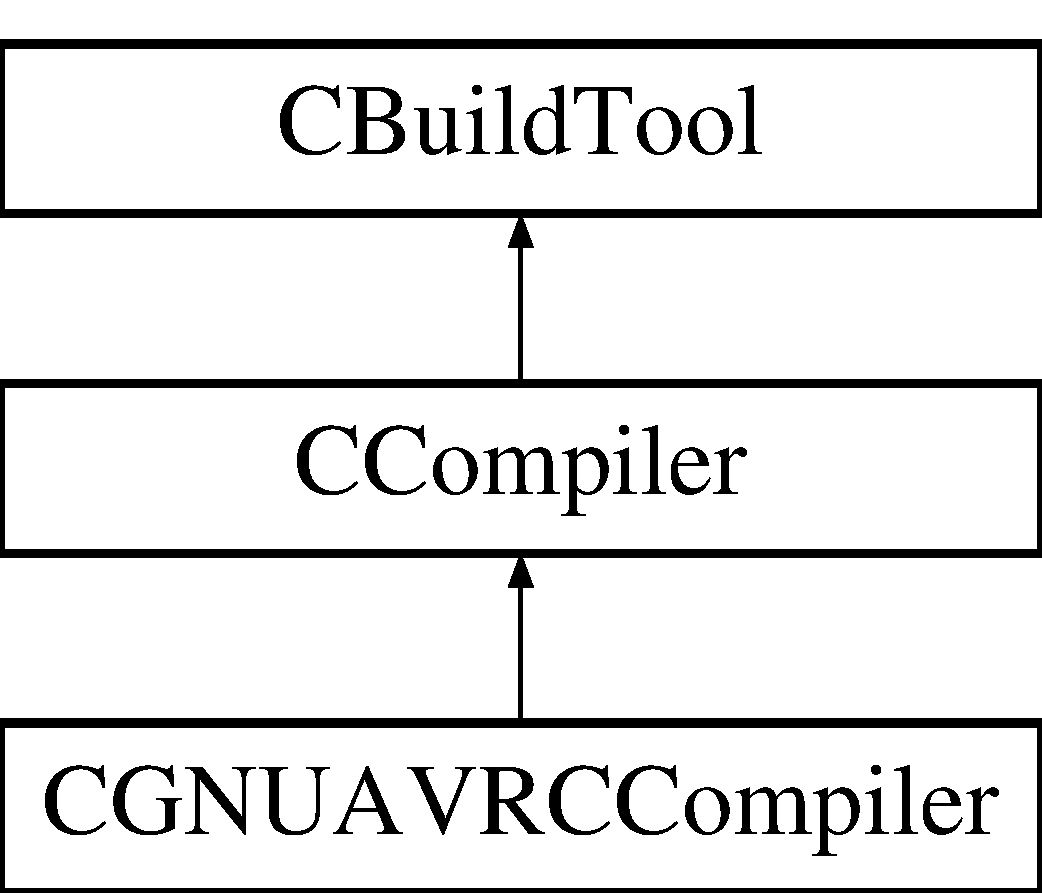
\includegraphics[height=3.000000cm]{da/d57/classCGNUAVRCCompiler}
\end{center}
\end{figure}
\subsection*{Public Member Functions}
\begin{DoxyCompactItemize}
\item 
virtual \hyperlink{classCIncludeSearchFilter}{C\-Include\-Search\-Filter} $\ast$ \hyperlink{classCGNUAVRCCompiler_a278ccc28910fb9cb8a20587bd966cf55}{Include\-Search\-Filter} (void) const 
\item 
virtual \hyperlink{classCGNUAVRCCompiler}{C\-G\-N\-U\-A\-V\-R\-C\-Compiler} $\ast$ \hyperlink{classCGNUAVRCCompiler_ad5630a463e0a41b5ecf28295f2c16e2f}{Create\-Instance} (void)
\item 
virtual void \hyperlink{classCGNUAVRCCompiler_a7f1f5abcd42d933e732c33bae1e18763}{Reset} (const \hyperlink{classCPlatform_a2fb735c63c53052f79629e338bb0f535}{C\-Platform\-::\-O\-S\-\_\-\-Type} O\-S)
\item 
\hyperlink{classCGNUAVRCCompiler_a467f142114353953863ad9bf449e1d77}{C\-G\-N\-U\-A\-V\-R\-C\-Compiler} (void)
\end{DoxyCompactItemize}
\subsection*{Private Attributes}
\begin{DoxyCompactItemize}
\item 
\hyperlink{classCCppIncludeSearchFilter}{C\-Cpp\-Include\-Search\-Filter} \hyperlink{classCGNUAVRCCompiler_a13660a7280c7109415125bbe4641246b}{m\-\_\-\-Include\-Search\-Filter}
\end{DoxyCompactItemize}
\subsection*{Additional Inherited Members}


\subsection{Constructor \& Destructor Documentation}
\hypertarget{classCGNUAVRCCompiler_a467f142114353953863ad9bf449e1d77}{\index{C\-G\-N\-U\-A\-V\-R\-C\-Compiler@{C\-G\-N\-U\-A\-V\-R\-C\-Compiler}!C\-G\-N\-U\-A\-V\-R\-C\-Compiler@{C\-G\-N\-U\-A\-V\-R\-C\-Compiler}}
\index{C\-G\-N\-U\-A\-V\-R\-C\-Compiler@{C\-G\-N\-U\-A\-V\-R\-C\-Compiler}!CGNUAVRCCompiler@{C\-G\-N\-U\-A\-V\-R\-C\-Compiler}}
\subsubsection[{C\-G\-N\-U\-A\-V\-R\-C\-Compiler}]{\setlength{\rightskip}{0pt plus 5cm}C\-G\-N\-U\-A\-V\-R\-C\-Compiler\-::\-C\-G\-N\-U\-A\-V\-R\-C\-Compiler (
\begin{DoxyParamCaption}
\item[{void}]{}
\end{DoxyParamCaption}
)}}\label{classCGNUAVRCCompiler_a467f142114353953863ad9bf449e1d77}


\subsection{Member Function Documentation}
\hypertarget{classCGNUAVRCCompiler_ad5630a463e0a41b5ecf28295f2c16e2f}{\index{C\-G\-N\-U\-A\-V\-R\-C\-Compiler@{C\-G\-N\-U\-A\-V\-R\-C\-Compiler}!Create\-Instance@{Create\-Instance}}
\index{Create\-Instance@{Create\-Instance}!CGNUAVRCCompiler@{C\-G\-N\-U\-A\-V\-R\-C\-Compiler}}
\subsubsection[{Create\-Instance}]{\setlength{\rightskip}{0pt plus 5cm}{\bf C\-G\-N\-U\-A\-V\-R\-C\-Compiler} $\ast$ C\-G\-N\-U\-A\-V\-R\-C\-Compiler\-::\-Create\-Instance (
\begin{DoxyParamCaption}
\item[{void}]{}
\end{DoxyParamCaption}
)\hspace{0.3cm}{\ttfamily [virtual]}}}\label{classCGNUAVRCCompiler_ad5630a463e0a41b5ecf28295f2c16e2f}


Reimplemented from \hyperlink{classCCompiler_a3d4aaaf69e1ba6070c729fd042d90012}{C\-Compiler}.

\hypertarget{classCGNUAVRCCompiler_a278ccc28910fb9cb8a20587bd966cf55}{\index{C\-G\-N\-U\-A\-V\-R\-C\-Compiler@{C\-G\-N\-U\-A\-V\-R\-C\-Compiler}!Include\-Search\-Filter@{Include\-Search\-Filter}}
\index{Include\-Search\-Filter@{Include\-Search\-Filter}!CGNUAVRCCompiler@{C\-G\-N\-U\-A\-V\-R\-C\-Compiler}}
\subsubsection[{Include\-Search\-Filter}]{\setlength{\rightskip}{0pt plus 5cm}{\bf C\-Include\-Search\-Filter} $\ast$ C\-G\-N\-U\-A\-V\-R\-C\-Compiler\-::\-Include\-Search\-Filter (
\begin{DoxyParamCaption}
\item[{void}]{}
\end{DoxyParamCaption}
) const\hspace{0.3cm}{\ttfamily [virtual]}}}\label{classCGNUAVRCCompiler_a278ccc28910fb9cb8a20587bd966cf55}


Reimplemented from \hyperlink{classCCompiler_a1dc477f47e953ddd4c653f3ba85c5468}{C\-Compiler}.

\hypertarget{classCGNUAVRCCompiler_a7f1f5abcd42d933e732c33bae1e18763}{\index{C\-G\-N\-U\-A\-V\-R\-C\-Compiler@{C\-G\-N\-U\-A\-V\-R\-C\-Compiler}!Reset@{Reset}}
\index{Reset@{Reset}!CGNUAVRCCompiler@{C\-G\-N\-U\-A\-V\-R\-C\-Compiler}}
\subsubsection[{Reset}]{\setlength{\rightskip}{0pt plus 5cm}void C\-G\-N\-U\-A\-V\-R\-C\-Compiler\-::\-Reset (
\begin{DoxyParamCaption}
\item[{const {\bf C\-Platform\-::\-O\-S\-\_\-\-Type}}]{O\-S}
\end{DoxyParamCaption}
)\hspace{0.3cm}{\ttfamily [virtual]}}}\label{classCGNUAVRCCompiler_a7f1f5abcd42d933e732c33bae1e18763}


Reimplemented from \hyperlink{classCBuildTool_abea21a0e61ab2177effdff5aaa169585}{C\-Build\-Tool}.



\subsection{Member Data Documentation}
\hypertarget{classCGNUAVRCCompiler_a13660a7280c7109415125bbe4641246b}{\index{C\-G\-N\-U\-A\-V\-R\-C\-Compiler@{C\-G\-N\-U\-A\-V\-R\-C\-Compiler}!m\-\_\-\-Include\-Search\-Filter@{m\-\_\-\-Include\-Search\-Filter}}
\index{m\-\_\-\-Include\-Search\-Filter@{m\-\_\-\-Include\-Search\-Filter}!CGNUAVRCCompiler@{C\-G\-N\-U\-A\-V\-R\-C\-Compiler}}
\subsubsection[{m\-\_\-\-Include\-Search\-Filter}]{\setlength{\rightskip}{0pt plus 5cm}{\bf C\-Cpp\-Include\-Search\-Filter} C\-G\-N\-U\-A\-V\-R\-C\-Compiler\-::m\-\_\-\-Include\-Search\-Filter\hspace{0.3cm}{\ttfamily [private]}}}\label{classCGNUAVRCCompiler_a13660a7280c7109415125bbe4641246b}


The documentation for this class was generated from the following files\-:\begin{DoxyCompactItemize}
\item 
src/\hyperlink{buildtools_8h}{buildtools.\-h}\item 
src/\hyperlink{buildtools_8cpp}{buildtools.\-cpp}\end{DoxyCompactItemize}

\hypertarget{classCGNUAVRCppCompiler}{\section{C\-G\-N\-U\-A\-V\-R\-Cpp\-Compiler Class Reference}
\label{classCGNUAVRCppCompiler}\index{C\-G\-N\-U\-A\-V\-R\-Cpp\-Compiler@{C\-G\-N\-U\-A\-V\-R\-Cpp\-Compiler}}
}


{\ttfamily \#include $<$buildtools.\-h$>$}

Inheritance diagram for C\-G\-N\-U\-A\-V\-R\-Cpp\-Compiler\-:\begin{figure}[H]
\begin{center}
\leavevmode
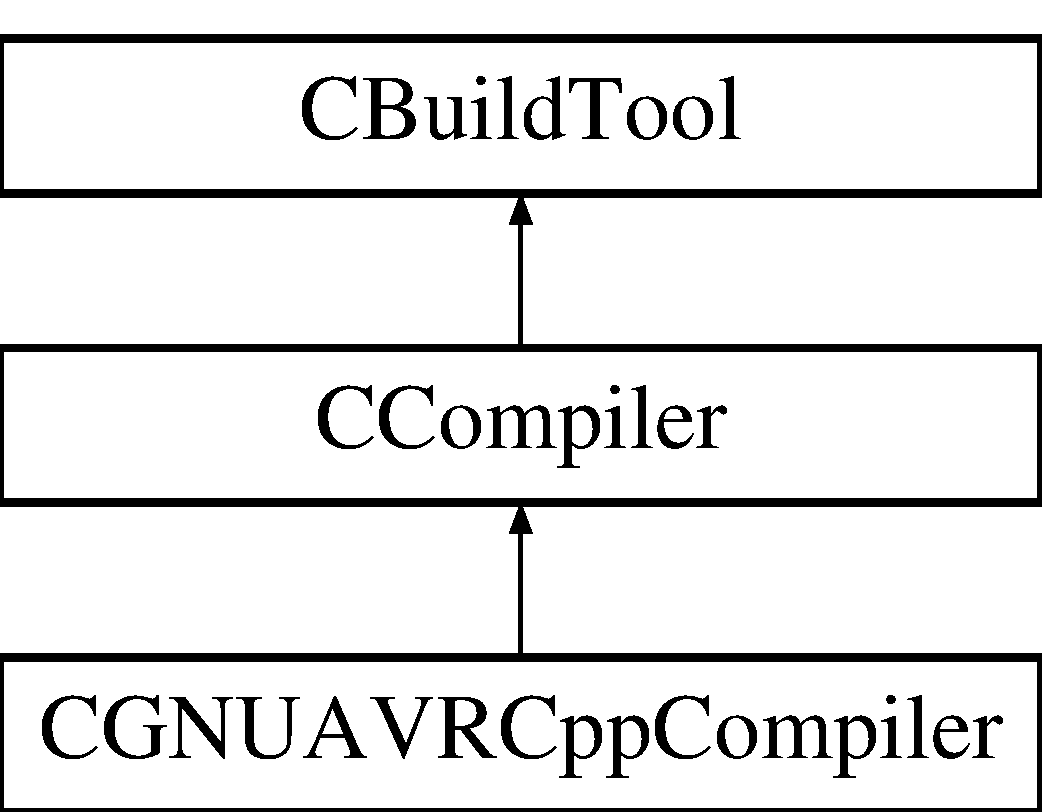
\includegraphics[height=3.000000cm]{d3/de1/classCGNUAVRCppCompiler}
\end{center}
\end{figure}
\subsection*{Public Member Functions}
\begin{DoxyCompactItemize}
\item 
virtual \hyperlink{classCIncludeSearchFilter}{C\-Include\-Search\-Filter} $\ast$ \hyperlink{classCGNUAVRCppCompiler_aae41e83908ef6be8ae274f75fb6a1cbe}{Include\-Search\-Filter} (void) const 
\item 
virtual \hyperlink{classCGNUAVRCppCompiler}{C\-G\-N\-U\-A\-V\-R\-Cpp\-Compiler} $\ast$ \hyperlink{classCGNUAVRCppCompiler_ac38cdc207e9dce42f53fef90ebaa3b87}{Create\-Instance} (void)
\item 
virtual void \hyperlink{classCGNUAVRCppCompiler_a3c597b2862b70725bcbc2d518c90f7bd}{Reset} (const \hyperlink{classCPlatform_a2fb735c63c53052f79629e338bb0f535}{C\-Platform\-::\-O\-S\-\_\-\-Type} O\-S)
\item 
\hyperlink{classCGNUAVRCppCompiler_aad034948d78174a0bbaa388d6ae7f4c5}{C\-G\-N\-U\-A\-V\-R\-Cpp\-Compiler} (void)
\end{DoxyCompactItemize}
\subsection*{Private Attributes}
\begin{DoxyCompactItemize}
\item 
\hyperlink{classCCppIncludeSearchFilter}{C\-Cpp\-Include\-Search\-Filter} \hyperlink{classCGNUAVRCppCompiler_aa6e99a6249279f771b338b09697f17ec}{m\-\_\-\-Include\-Search\-Filter}
\end{DoxyCompactItemize}
\subsection*{Additional Inherited Members}


\subsection{Constructor \& Destructor Documentation}
\hypertarget{classCGNUAVRCppCompiler_aad034948d78174a0bbaa388d6ae7f4c5}{\index{C\-G\-N\-U\-A\-V\-R\-Cpp\-Compiler@{C\-G\-N\-U\-A\-V\-R\-Cpp\-Compiler}!C\-G\-N\-U\-A\-V\-R\-Cpp\-Compiler@{C\-G\-N\-U\-A\-V\-R\-Cpp\-Compiler}}
\index{C\-G\-N\-U\-A\-V\-R\-Cpp\-Compiler@{C\-G\-N\-U\-A\-V\-R\-Cpp\-Compiler}!CGNUAVRCppCompiler@{C\-G\-N\-U\-A\-V\-R\-Cpp\-Compiler}}
\subsubsection[{C\-G\-N\-U\-A\-V\-R\-Cpp\-Compiler}]{\setlength{\rightskip}{0pt plus 5cm}C\-G\-N\-U\-A\-V\-R\-Cpp\-Compiler\-::\-C\-G\-N\-U\-A\-V\-R\-Cpp\-Compiler (
\begin{DoxyParamCaption}
\item[{void}]{}
\end{DoxyParamCaption}
)}}\label{classCGNUAVRCppCompiler_aad034948d78174a0bbaa388d6ae7f4c5}


\subsection{Member Function Documentation}
\hypertarget{classCGNUAVRCppCompiler_ac38cdc207e9dce42f53fef90ebaa3b87}{\index{C\-G\-N\-U\-A\-V\-R\-Cpp\-Compiler@{C\-G\-N\-U\-A\-V\-R\-Cpp\-Compiler}!Create\-Instance@{Create\-Instance}}
\index{Create\-Instance@{Create\-Instance}!CGNUAVRCppCompiler@{C\-G\-N\-U\-A\-V\-R\-Cpp\-Compiler}}
\subsubsection[{Create\-Instance}]{\setlength{\rightskip}{0pt plus 5cm}{\bf C\-G\-N\-U\-A\-V\-R\-Cpp\-Compiler} $\ast$ C\-G\-N\-U\-A\-V\-R\-Cpp\-Compiler\-::\-Create\-Instance (
\begin{DoxyParamCaption}
\item[{void}]{}
\end{DoxyParamCaption}
)\hspace{0.3cm}{\ttfamily [virtual]}}}\label{classCGNUAVRCppCompiler_ac38cdc207e9dce42f53fef90ebaa3b87}


Reimplemented from \hyperlink{classCCompiler_a3d4aaaf69e1ba6070c729fd042d90012}{C\-Compiler}.

\hypertarget{classCGNUAVRCppCompiler_aae41e83908ef6be8ae274f75fb6a1cbe}{\index{C\-G\-N\-U\-A\-V\-R\-Cpp\-Compiler@{C\-G\-N\-U\-A\-V\-R\-Cpp\-Compiler}!Include\-Search\-Filter@{Include\-Search\-Filter}}
\index{Include\-Search\-Filter@{Include\-Search\-Filter}!CGNUAVRCppCompiler@{C\-G\-N\-U\-A\-V\-R\-Cpp\-Compiler}}
\subsubsection[{Include\-Search\-Filter}]{\setlength{\rightskip}{0pt plus 5cm}{\bf C\-Include\-Search\-Filter} $\ast$ C\-G\-N\-U\-A\-V\-R\-Cpp\-Compiler\-::\-Include\-Search\-Filter (
\begin{DoxyParamCaption}
\item[{void}]{}
\end{DoxyParamCaption}
) const\hspace{0.3cm}{\ttfamily [virtual]}}}\label{classCGNUAVRCppCompiler_aae41e83908ef6be8ae274f75fb6a1cbe}


Reimplemented from \hyperlink{classCCompiler_a1dc477f47e953ddd4c653f3ba85c5468}{C\-Compiler}.

\hypertarget{classCGNUAVRCppCompiler_a3c597b2862b70725bcbc2d518c90f7bd}{\index{C\-G\-N\-U\-A\-V\-R\-Cpp\-Compiler@{C\-G\-N\-U\-A\-V\-R\-Cpp\-Compiler}!Reset@{Reset}}
\index{Reset@{Reset}!CGNUAVRCppCompiler@{C\-G\-N\-U\-A\-V\-R\-Cpp\-Compiler}}
\subsubsection[{Reset}]{\setlength{\rightskip}{0pt plus 5cm}void C\-G\-N\-U\-A\-V\-R\-Cpp\-Compiler\-::\-Reset (
\begin{DoxyParamCaption}
\item[{const {\bf C\-Platform\-::\-O\-S\-\_\-\-Type}}]{O\-S}
\end{DoxyParamCaption}
)\hspace{0.3cm}{\ttfamily [virtual]}}}\label{classCGNUAVRCppCompiler_a3c597b2862b70725bcbc2d518c90f7bd}


Reimplemented from \hyperlink{classCBuildTool_abea21a0e61ab2177effdff5aaa169585}{C\-Build\-Tool}.



\subsection{Member Data Documentation}
\hypertarget{classCGNUAVRCppCompiler_aa6e99a6249279f771b338b09697f17ec}{\index{C\-G\-N\-U\-A\-V\-R\-Cpp\-Compiler@{C\-G\-N\-U\-A\-V\-R\-Cpp\-Compiler}!m\-\_\-\-Include\-Search\-Filter@{m\-\_\-\-Include\-Search\-Filter}}
\index{m\-\_\-\-Include\-Search\-Filter@{m\-\_\-\-Include\-Search\-Filter}!CGNUAVRCppCompiler@{C\-G\-N\-U\-A\-V\-R\-Cpp\-Compiler}}
\subsubsection[{m\-\_\-\-Include\-Search\-Filter}]{\setlength{\rightskip}{0pt plus 5cm}{\bf C\-Cpp\-Include\-Search\-Filter} C\-G\-N\-U\-A\-V\-R\-Cpp\-Compiler\-::m\-\_\-\-Include\-Search\-Filter\hspace{0.3cm}{\ttfamily [private]}}}\label{classCGNUAVRCppCompiler_aa6e99a6249279f771b338b09697f17ec}


The documentation for this class was generated from the following files\-:\begin{DoxyCompactItemize}
\item 
src/\hyperlink{buildtools_8h}{buildtools.\-h}\item 
src/\hyperlink{buildtools_8cpp}{buildtools.\-cpp}\end{DoxyCompactItemize}

\hypertarget{classCGNUAVRDependencyGenerator}{\section{C\-G\-N\-U\-A\-V\-R\-Dependency\-Generator Class Reference}
\label{classCGNUAVRDependencyGenerator}\index{C\-G\-N\-U\-A\-V\-R\-Dependency\-Generator@{C\-G\-N\-U\-A\-V\-R\-Dependency\-Generator}}
}


{\ttfamily \#include $<$buildtools.\-h$>$}

Inheritance diagram for C\-G\-N\-U\-A\-V\-R\-Dependency\-Generator\-:\begin{figure}[H]
\begin{center}
\leavevmode
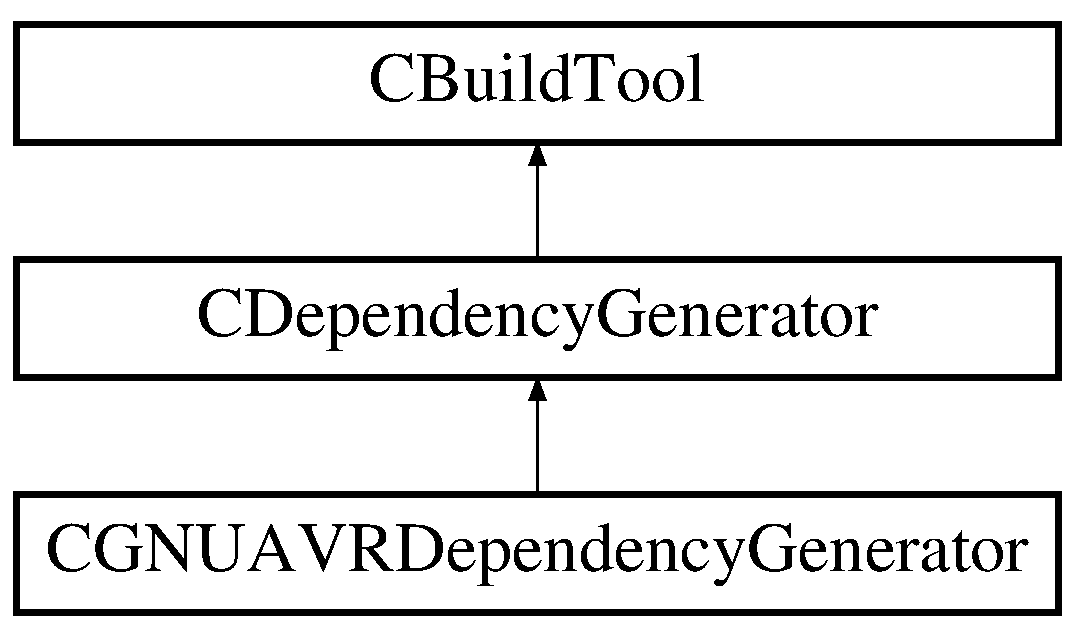
\includegraphics[height=3.000000cm]{d6/d35/classCGNUAVRDependencyGenerator}
\end{center}
\end{figure}
\subsection*{Public Member Functions}
\begin{DoxyCompactItemize}
\item 
virtual \hyperlink{classCDependencyGenerator}{C\-Dependency\-Generator} $\ast$ \hyperlink{classCGNUAVRDependencyGenerator_a5d4d5e45d1cdd58d998ac961a66647dc}{Create\-Instance} (void)
\item 
virtual void \hyperlink{classCGNUAVRDependencyGenerator_af96f3eb85393be62b8b91f0376b17273}{Reset} (const \hyperlink{classCPlatform_a2fb735c63c53052f79629e338bb0f535}{C\-Platform\-::\-O\-S\-\_\-\-Type} O\-S)
\item 
\hyperlink{classCGNUAVRDependencyGenerator_ae21ae7f52c6f2ac00754297adf953e27}{C\-G\-N\-U\-A\-V\-R\-Dependency\-Generator} (void)
\end{DoxyCompactItemize}
\subsection*{Additional Inherited Members}


\subsection{Constructor \& Destructor Documentation}
\hypertarget{classCGNUAVRDependencyGenerator_ae21ae7f52c6f2ac00754297adf953e27}{\index{C\-G\-N\-U\-A\-V\-R\-Dependency\-Generator@{C\-G\-N\-U\-A\-V\-R\-Dependency\-Generator}!C\-G\-N\-U\-A\-V\-R\-Dependency\-Generator@{C\-G\-N\-U\-A\-V\-R\-Dependency\-Generator}}
\index{C\-G\-N\-U\-A\-V\-R\-Dependency\-Generator@{C\-G\-N\-U\-A\-V\-R\-Dependency\-Generator}!CGNUAVRDependencyGenerator@{C\-G\-N\-U\-A\-V\-R\-Dependency\-Generator}}
\subsubsection[{C\-G\-N\-U\-A\-V\-R\-Dependency\-Generator}]{\setlength{\rightskip}{0pt plus 5cm}C\-G\-N\-U\-A\-V\-R\-Dependency\-Generator\-::\-C\-G\-N\-U\-A\-V\-R\-Dependency\-Generator (
\begin{DoxyParamCaption}
\item[{void}]{}
\end{DoxyParamCaption}
)}}\label{classCGNUAVRDependencyGenerator_ae21ae7f52c6f2ac00754297adf953e27}


\subsection{Member Function Documentation}
\hypertarget{classCGNUAVRDependencyGenerator_a5d4d5e45d1cdd58d998ac961a66647dc}{\index{C\-G\-N\-U\-A\-V\-R\-Dependency\-Generator@{C\-G\-N\-U\-A\-V\-R\-Dependency\-Generator}!Create\-Instance@{Create\-Instance}}
\index{Create\-Instance@{Create\-Instance}!CGNUAVRDependencyGenerator@{C\-G\-N\-U\-A\-V\-R\-Dependency\-Generator}}
\subsubsection[{Create\-Instance}]{\setlength{\rightskip}{0pt plus 5cm}{\bf C\-Dependency\-Generator} $\ast$ C\-G\-N\-U\-A\-V\-R\-Dependency\-Generator\-::\-Create\-Instance (
\begin{DoxyParamCaption}
\item[{void}]{}
\end{DoxyParamCaption}
)\hspace{0.3cm}{\ttfamily [virtual]}}}\label{classCGNUAVRDependencyGenerator_a5d4d5e45d1cdd58d998ac961a66647dc}


Reimplemented from \hyperlink{classCDependencyGenerator_af25a1710b95578b0e7ebcec02c4a7238}{C\-Dependency\-Generator}.

\hypertarget{classCGNUAVRDependencyGenerator_af96f3eb85393be62b8b91f0376b17273}{\index{C\-G\-N\-U\-A\-V\-R\-Dependency\-Generator@{C\-G\-N\-U\-A\-V\-R\-Dependency\-Generator}!Reset@{Reset}}
\index{Reset@{Reset}!CGNUAVRDependencyGenerator@{C\-G\-N\-U\-A\-V\-R\-Dependency\-Generator}}
\subsubsection[{Reset}]{\setlength{\rightskip}{0pt plus 5cm}void C\-G\-N\-U\-A\-V\-R\-Dependency\-Generator\-::\-Reset (
\begin{DoxyParamCaption}
\item[{const {\bf C\-Platform\-::\-O\-S\-\_\-\-Type}}]{O\-S}
\end{DoxyParamCaption}
)\hspace{0.3cm}{\ttfamily [virtual]}}}\label{classCGNUAVRDependencyGenerator_af96f3eb85393be62b8b91f0376b17273}


Reimplemented from \hyperlink{classCBuildTool_abea21a0e61ab2177effdff5aaa169585}{C\-Build\-Tool}.



The documentation for this class was generated from the following files\-:\begin{DoxyCompactItemize}
\item 
src/\hyperlink{buildtools_8h}{buildtools.\-h}\item 
src/\hyperlink{buildtools_8cpp}{buildtools.\-cpp}\end{DoxyCompactItemize}

\hypertarget{classCGNUAVRDynamicLinker}{\section{C\-G\-N\-U\-A\-V\-R\-Dynamic\-Linker Class Reference}
\label{classCGNUAVRDynamicLinker}\index{C\-G\-N\-U\-A\-V\-R\-Dynamic\-Linker@{C\-G\-N\-U\-A\-V\-R\-Dynamic\-Linker}}
}


{\ttfamily \#include $<$buildtools.\-h$>$}

Inheritance diagram for C\-G\-N\-U\-A\-V\-R\-Dynamic\-Linker\-:\begin{figure}[H]
\begin{center}
\leavevmode
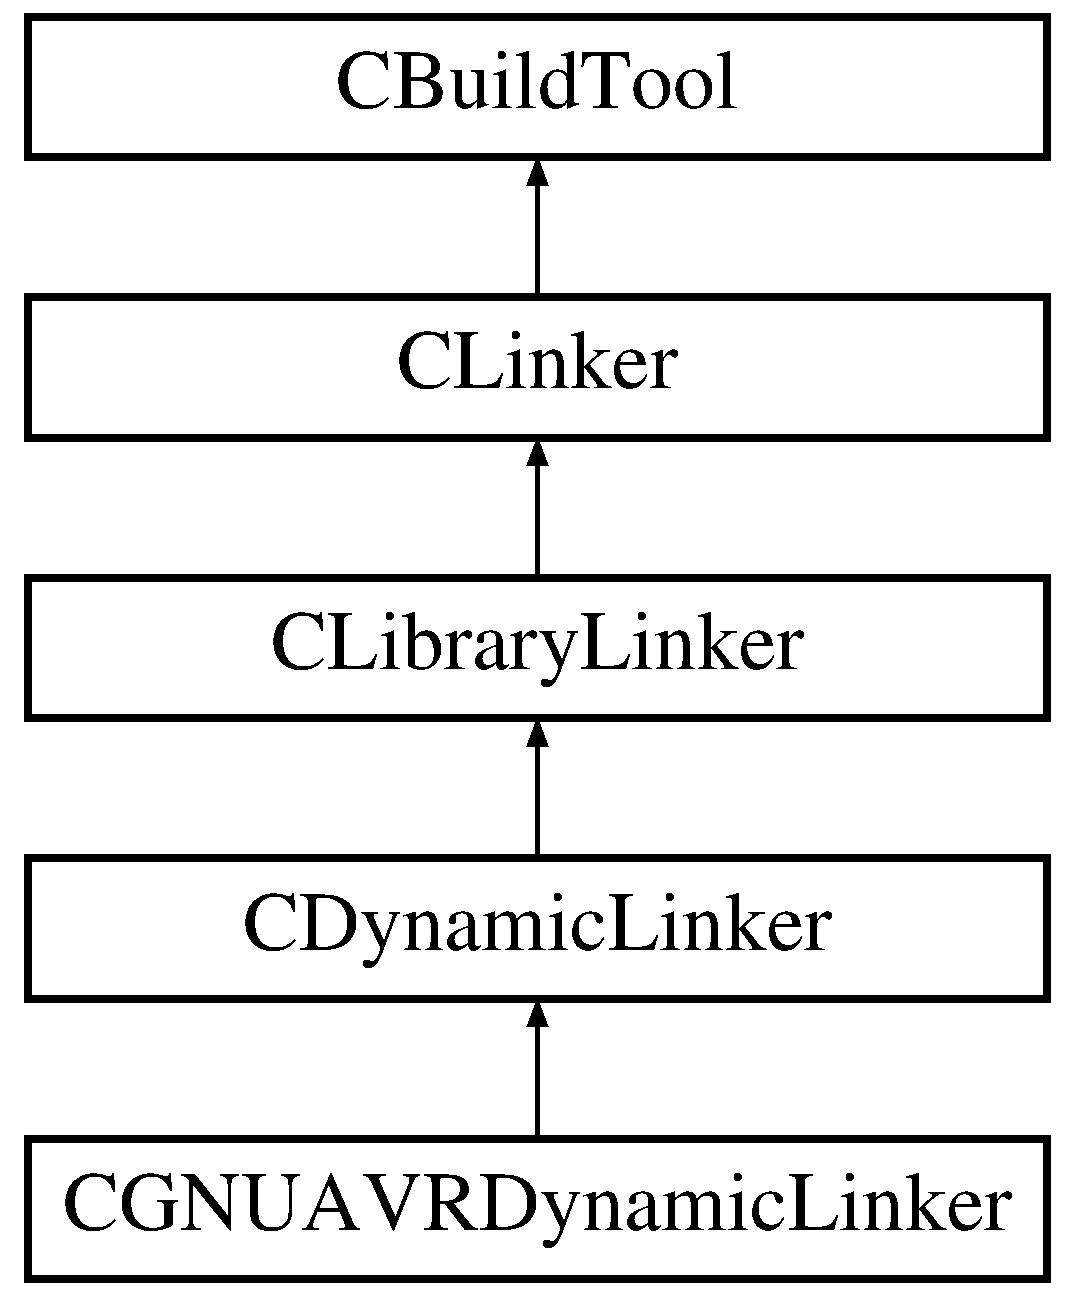
\includegraphics[height=5.000000cm]{df/d14/classCGNUAVRDynamicLinker}
\end{center}
\end{figure}
\subsection*{Public Member Functions}
\begin{DoxyCompactItemize}
\item 
virtual \hyperlink{classCGNUAVRDynamicLinker}{C\-G\-N\-U\-A\-V\-R\-Dynamic\-Linker} $\ast$ \hyperlink{classCGNUAVRDynamicLinker_ae26802d4ce8ce7c45a87a65bf7066832}{Create\-Instance} (void)
\item 
virtual void \hyperlink{classCGNUAVRDynamicLinker_a08c53dfc9f1352a486bfb736aee544f4}{Reset} (const \hyperlink{classCPlatform_a2fb735c63c53052f79629e338bb0f535}{C\-Platform\-::\-O\-S\-\_\-\-Type} O\-S)
\item 
\hyperlink{classCGNUAVRDynamicLinker_ab276746cda988d5147c1b8e1215a9cb6}{C\-G\-N\-U\-A\-V\-R\-Dynamic\-Linker} (void)
\end{DoxyCompactItemize}
\subsection*{Additional Inherited Members}


\subsection{Constructor \& Destructor Documentation}
\hypertarget{classCGNUAVRDynamicLinker_ab276746cda988d5147c1b8e1215a9cb6}{\index{C\-G\-N\-U\-A\-V\-R\-Dynamic\-Linker@{C\-G\-N\-U\-A\-V\-R\-Dynamic\-Linker}!C\-G\-N\-U\-A\-V\-R\-Dynamic\-Linker@{C\-G\-N\-U\-A\-V\-R\-Dynamic\-Linker}}
\index{C\-G\-N\-U\-A\-V\-R\-Dynamic\-Linker@{C\-G\-N\-U\-A\-V\-R\-Dynamic\-Linker}!CGNUAVRDynamicLinker@{C\-G\-N\-U\-A\-V\-R\-Dynamic\-Linker}}
\subsubsection[{C\-G\-N\-U\-A\-V\-R\-Dynamic\-Linker}]{\setlength{\rightskip}{0pt plus 5cm}C\-G\-N\-U\-A\-V\-R\-Dynamic\-Linker\-::\-C\-G\-N\-U\-A\-V\-R\-Dynamic\-Linker (
\begin{DoxyParamCaption}
\item[{void}]{}
\end{DoxyParamCaption}
)}}\label{classCGNUAVRDynamicLinker_ab276746cda988d5147c1b8e1215a9cb6}


\subsection{Member Function Documentation}
\hypertarget{classCGNUAVRDynamicLinker_ae26802d4ce8ce7c45a87a65bf7066832}{\index{C\-G\-N\-U\-A\-V\-R\-Dynamic\-Linker@{C\-G\-N\-U\-A\-V\-R\-Dynamic\-Linker}!Create\-Instance@{Create\-Instance}}
\index{Create\-Instance@{Create\-Instance}!CGNUAVRDynamicLinker@{C\-G\-N\-U\-A\-V\-R\-Dynamic\-Linker}}
\subsubsection[{Create\-Instance}]{\setlength{\rightskip}{0pt plus 5cm}{\bf C\-G\-N\-U\-A\-V\-R\-Dynamic\-Linker} $\ast$ C\-G\-N\-U\-A\-V\-R\-Dynamic\-Linker\-::\-Create\-Instance (
\begin{DoxyParamCaption}
\item[{void}]{}
\end{DoxyParamCaption}
)\hspace{0.3cm}{\ttfamily [virtual]}}}\label{classCGNUAVRDynamicLinker_ae26802d4ce8ce7c45a87a65bf7066832}


Reimplemented from \hyperlink{classCDynamicLinker_ac71406ca5c6e8e991a6418a6307d274c}{C\-Dynamic\-Linker}.

\hypertarget{classCGNUAVRDynamicLinker_a08c53dfc9f1352a486bfb736aee544f4}{\index{C\-G\-N\-U\-A\-V\-R\-Dynamic\-Linker@{C\-G\-N\-U\-A\-V\-R\-Dynamic\-Linker}!Reset@{Reset}}
\index{Reset@{Reset}!CGNUAVRDynamicLinker@{C\-G\-N\-U\-A\-V\-R\-Dynamic\-Linker}}
\subsubsection[{Reset}]{\setlength{\rightskip}{0pt plus 5cm}void C\-G\-N\-U\-A\-V\-R\-Dynamic\-Linker\-::\-Reset (
\begin{DoxyParamCaption}
\item[{const {\bf C\-Platform\-::\-O\-S\-\_\-\-Type}}]{O\-S}
\end{DoxyParamCaption}
)\hspace{0.3cm}{\ttfamily [virtual]}}}\label{classCGNUAVRDynamicLinker_a08c53dfc9f1352a486bfb736aee544f4}


Reimplemented from \hyperlink{classCDynamicLinker_a437d46ee65b3585e7be9d15d40c26820}{C\-Dynamic\-Linker}.



The documentation for this class was generated from the following files\-:\begin{DoxyCompactItemize}
\item 
src/\hyperlink{buildtools_8h}{buildtools.\-h}\item 
src/\hyperlink{buildtools_8cpp}{buildtools.\-cpp}\end{DoxyCompactItemize}

\hypertarget{classCGNUAVRExecutableLinker}{\section{C\-G\-N\-U\-A\-V\-R\-Executable\-Linker Class Reference}
\label{classCGNUAVRExecutableLinker}\index{C\-G\-N\-U\-A\-V\-R\-Executable\-Linker@{C\-G\-N\-U\-A\-V\-R\-Executable\-Linker}}
}


{\ttfamily \#include $<$buildtools.\-h$>$}

Inheritance diagram for C\-G\-N\-U\-A\-V\-R\-Executable\-Linker\-:\begin{figure}[H]
\begin{center}
\leavevmode
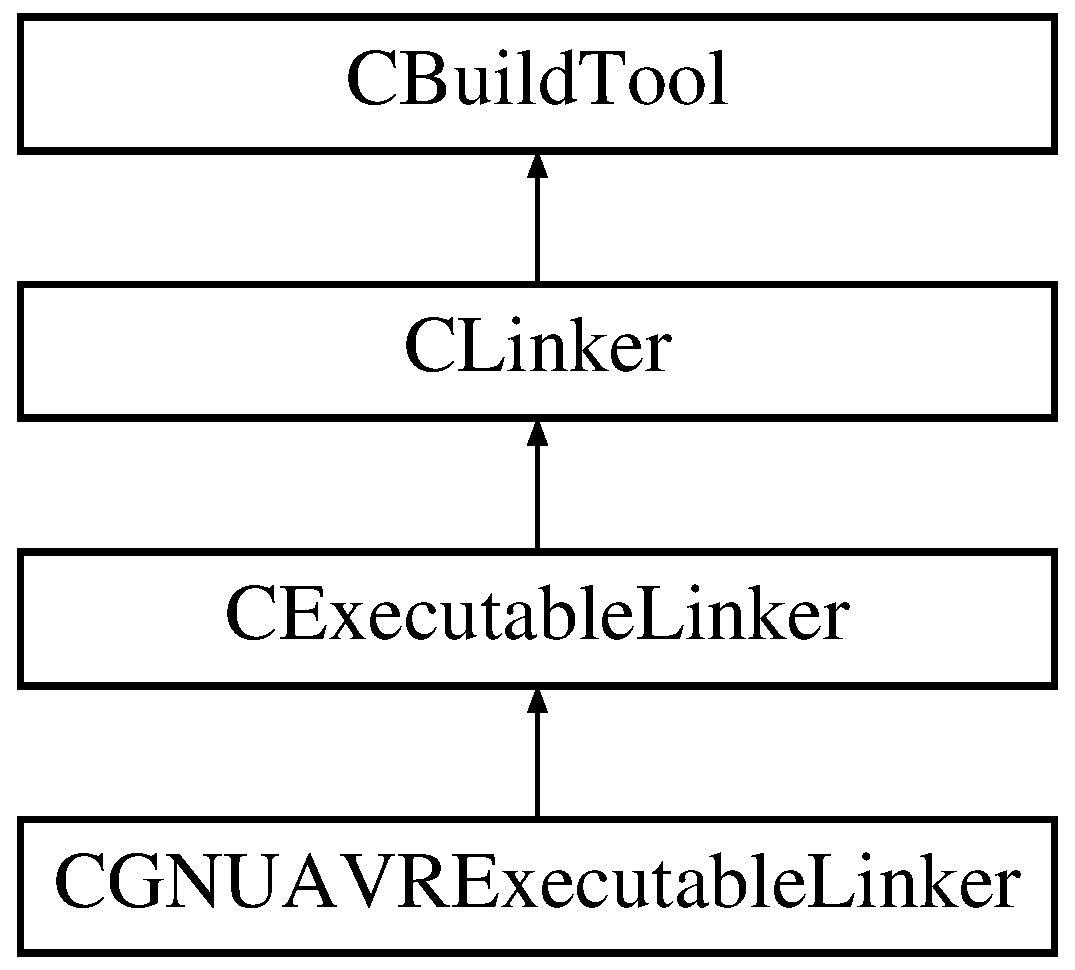
\includegraphics[height=4.000000cm]{df/d66/classCGNUAVRExecutableLinker}
\end{center}
\end{figure}
\subsection*{Public Member Functions}
\begin{DoxyCompactItemize}
\item 
virtual \hyperlink{classCGNUAVRExecutableLinker}{C\-G\-N\-U\-A\-V\-R\-Executable\-Linker} $\ast$ \hyperlink{classCGNUAVRExecutableLinker_ad6c7693277ecb00d550bde8e1bda0b8c}{Create\-Instance} (void)
\item 
virtual void \hyperlink{classCGNUAVRExecutableLinker_a2bb4fb92e5d0d6846a8635e1ebcc9ccb}{Reset} (const \hyperlink{classCPlatform_a2fb735c63c53052f79629e338bb0f535}{C\-Platform\-::\-O\-S\-\_\-\-Type} O\-S)
\item 
\hyperlink{classCGNUAVRExecutableLinker_a32c345c1f901ab4eb7cce235bfecfd14}{C\-G\-N\-U\-A\-V\-R\-Executable\-Linker} (void)
\end{DoxyCompactItemize}
\subsection*{Additional Inherited Members}


\subsection{Constructor \& Destructor Documentation}
\hypertarget{classCGNUAVRExecutableLinker_a32c345c1f901ab4eb7cce235bfecfd14}{\index{C\-G\-N\-U\-A\-V\-R\-Executable\-Linker@{C\-G\-N\-U\-A\-V\-R\-Executable\-Linker}!C\-G\-N\-U\-A\-V\-R\-Executable\-Linker@{C\-G\-N\-U\-A\-V\-R\-Executable\-Linker}}
\index{C\-G\-N\-U\-A\-V\-R\-Executable\-Linker@{C\-G\-N\-U\-A\-V\-R\-Executable\-Linker}!CGNUAVRExecutableLinker@{C\-G\-N\-U\-A\-V\-R\-Executable\-Linker}}
\subsubsection[{C\-G\-N\-U\-A\-V\-R\-Executable\-Linker}]{\setlength{\rightskip}{0pt plus 5cm}C\-G\-N\-U\-A\-V\-R\-Executable\-Linker\-::\-C\-G\-N\-U\-A\-V\-R\-Executable\-Linker (
\begin{DoxyParamCaption}
\item[{void}]{}
\end{DoxyParamCaption}
)}}\label{classCGNUAVRExecutableLinker_a32c345c1f901ab4eb7cce235bfecfd14}


\subsection{Member Function Documentation}
\hypertarget{classCGNUAVRExecutableLinker_ad6c7693277ecb00d550bde8e1bda0b8c}{\index{C\-G\-N\-U\-A\-V\-R\-Executable\-Linker@{C\-G\-N\-U\-A\-V\-R\-Executable\-Linker}!Create\-Instance@{Create\-Instance}}
\index{Create\-Instance@{Create\-Instance}!CGNUAVRExecutableLinker@{C\-G\-N\-U\-A\-V\-R\-Executable\-Linker}}
\subsubsection[{Create\-Instance}]{\setlength{\rightskip}{0pt plus 5cm}{\bf C\-G\-N\-U\-A\-V\-R\-Executable\-Linker} $\ast$ C\-G\-N\-U\-A\-V\-R\-Executable\-Linker\-::\-Create\-Instance (
\begin{DoxyParamCaption}
\item[{void}]{}
\end{DoxyParamCaption}
)\hspace{0.3cm}{\ttfamily [virtual]}}}\label{classCGNUAVRExecutableLinker_ad6c7693277ecb00d550bde8e1bda0b8c}


Reimplemented from \hyperlink{classCExecutableLinker_a457b823b737b0a78285d5ede77df827c}{C\-Executable\-Linker}.

\hypertarget{classCGNUAVRExecutableLinker_a2bb4fb92e5d0d6846a8635e1ebcc9ccb}{\index{C\-G\-N\-U\-A\-V\-R\-Executable\-Linker@{C\-G\-N\-U\-A\-V\-R\-Executable\-Linker}!Reset@{Reset}}
\index{Reset@{Reset}!CGNUAVRExecutableLinker@{C\-G\-N\-U\-A\-V\-R\-Executable\-Linker}}
\subsubsection[{Reset}]{\setlength{\rightskip}{0pt plus 5cm}void C\-G\-N\-U\-A\-V\-R\-Executable\-Linker\-::\-Reset (
\begin{DoxyParamCaption}
\item[{const {\bf C\-Platform\-::\-O\-S\-\_\-\-Type}}]{O\-S}
\end{DoxyParamCaption}
)\hspace{0.3cm}{\ttfamily [virtual]}}}\label{classCGNUAVRExecutableLinker_a2bb4fb92e5d0d6846a8635e1ebcc9ccb}


Reimplemented from \hyperlink{classCBuildTool_abea21a0e61ab2177effdff5aaa169585}{C\-Build\-Tool}.



The documentation for this class was generated from the following files\-:\begin{DoxyCompactItemize}
\item 
src/\hyperlink{buildtools_8h}{buildtools.\-h}\item 
src/\hyperlink{buildtools_8cpp}{buildtools.\-cpp}\end{DoxyCompactItemize}

\hypertarget{classCGNUAVRStaticLinker}{\section{C\-G\-N\-U\-A\-V\-R\-Static\-Linker Class Reference}
\label{classCGNUAVRStaticLinker}\index{C\-G\-N\-U\-A\-V\-R\-Static\-Linker@{C\-G\-N\-U\-A\-V\-R\-Static\-Linker}}
}


{\ttfamily \#include $<$buildtools.\-h$>$}

Inheritance diagram for C\-G\-N\-U\-A\-V\-R\-Static\-Linker\-:\begin{figure}[H]
\begin{center}
\leavevmode
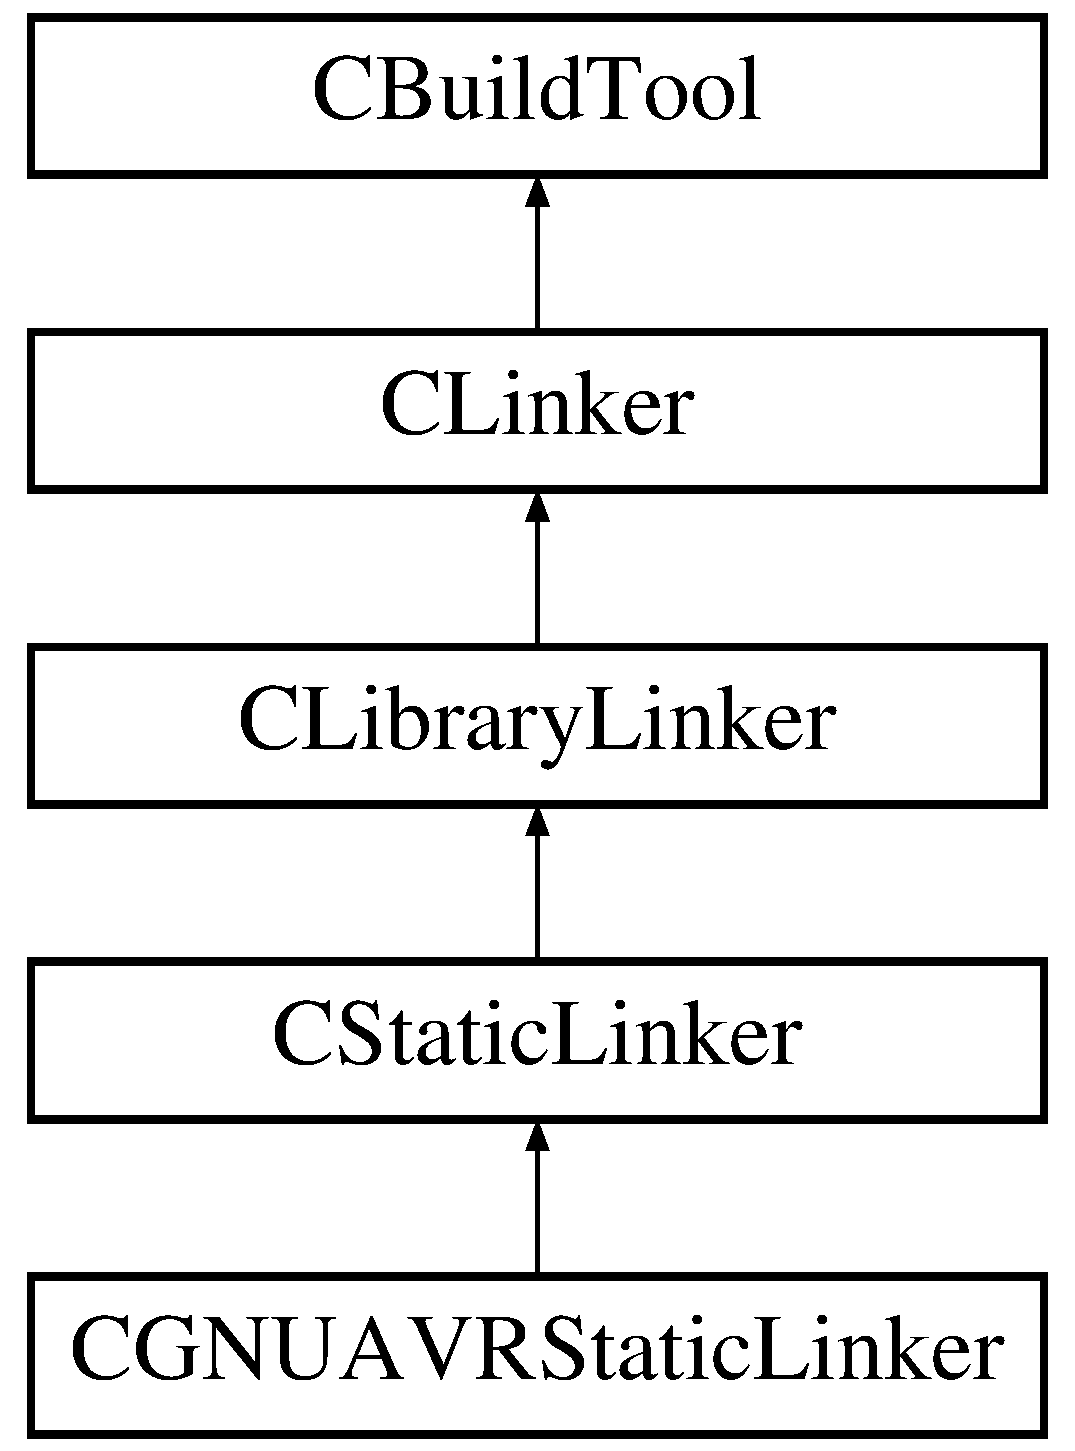
\includegraphics[height=5.000000cm]{d4/d81/classCGNUAVRStaticLinker}
\end{center}
\end{figure}
\subsection*{Public Member Functions}
\begin{DoxyCompactItemize}
\item 
virtual \hyperlink{classCGNUAVRStaticLinker}{C\-G\-N\-U\-A\-V\-R\-Static\-Linker} $\ast$ \hyperlink{classCGNUAVRStaticLinker_ad4852b66cb610455765089ff8fdb7771}{Create\-Instance} (void)
\item 
virtual void \hyperlink{classCGNUAVRStaticLinker_aed827fdf1de17dfdbcdfe0ba4ca55fda}{Reset} (const \hyperlink{classCPlatform_a2fb735c63c53052f79629e338bb0f535}{C\-Platform\-::\-O\-S\-\_\-\-Type} O\-S)
\item 
\hyperlink{classCGNUAVRStaticLinker_aeb77f35f17c0f84761ef1204c7e8e457}{C\-G\-N\-U\-A\-V\-R\-Static\-Linker} (void)
\end{DoxyCompactItemize}
\subsection*{Additional Inherited Members}


\subsection{Constructor \& Destructor Documentation}
\hypertarget{classCGNUAVRStaticLinker_aeb77f35f17c0f84761ef1204c7e8e457}{\index{C\-G\-N\-U\-A\-V\-R\-Static\-Linker@{C\-G\-N\-U\-A\-V\-R\-Static\-Linker}!C\-G\-N\-U\-A\-V\-R\-Static\-Linker@{C\-G\-N\-U\-A\-V\-R\-Static\-Linker}}
\index{C\-G\-N\-U\-A\-V\-R\-Static\-Linker@{C\-G\-N\-U\-A\-V\-R\-Static\-Linker}!CGNUAVRStaticLinker@{C\-G\-N\-U\-A\-V\-R\-Static\-Linker}}
\subsubsection[{C\-G\-N\-U\-A\-V\-R\-Static\-Linker}]{\setlength{\rightskip}{0pt plus 5cm}C\-G\-N\-U\-A\-V\-R\-Static\-Linker\-::\-C\-G\-N\-U\-A\-V\-R\-Static\-Linker (
\begin{DoxyParamCaption}
\item[{void}]{}
\end{DoxyParamCaption}
)}}\label{classCGNUAVRStaticLinker_aeb77f35f17c0f84761ef1204c7e8e457}


\subsection{Member Function Documentation}
\hypertarget{classCGNUAVRStaticLinker_ad4852b66cb610455765089ff8fdb7771}{\index{C\-G\-N\-U\-A\-V\-R\-Static\-Linker@{C\-G\-N\-U\-A\-V\-R\-Static\-Linker}!Create\-Instance@{Create\-Instance}}
\index{Create\-Instance@{Create\-Instance}!CGNUAVRStaticLinker@{C\-G\-N\-U\-A\-V\-R\-Static\-Linker}}
\subsubsection[{Create\-Instance}]{\setlength{\rightskip}{0pt plus 5cm}{\bf C\-G\-N\-U\-A\-V\-R\-Static\-Linker} $\ast$ C\-G\-N\-U\-A\-V\-R\-Static\-Linker\-::\-Create\-Instance (
\begin{DoxyParamCaption}
\item[{void}]{}
\end{DoxyParamCaption}
)\hspace{0.3cm}{\ttfamily [virtual]}}}\label{classCGNUAVRStaticLinker_ad4852b66cb610455765089ff8fdb7771}


Reimplemented from \hyperlink{classCStaticLinker_a7e626491caa847ef207032ee600625db}{C\-Static\-Linker}.

\hypertarget{classCGNUAVRStaticLinker_aed827fdf1de17dfdbcdfe0ba4ca55fda}{\index{C\-G\-N\-U\-A\-V\-R\-Static\-Linker@{C\-G\-N\-U\-A\-V\-R\-Static\-Linker}!Reset@{Reset}}
\index{Reset@{Reset}!CGNUAVRStaticLinker@{C\-G\-N\-U\-A\-V\-R\-Static\-Linker}}
\subsubsection[{Reset}]{\setlength{\rightskip}{0pt plus 5cm}void C\-G\-N\-U\-A\-V\-R\-Static\-Linker\-::\-Reset (
\begin{DoxyParamCaption}
\item[{const {\bf C\-Platform\-::\-O\-S\-\_\-\-Type}}]{O\-S}
\end{DoxyParamCaption}
)\hspace{0.3cm}{\ttfamily [virtual]}}}\label{classCGNUAVRStaticLinker_aed827fdf1de17dfdbcdfe0ba4ca55fda}


Reimplemented from \hyperlink{classCBuildTool_abea21a0e61ab2177effdff5aaa169585}{C\-Build\-Tool}.



The documentation for this class was generated from the following files\-:\begin{DoxyCompactItemize}
\item 
src/\hyperlink{buildtools_8h}{buildtools.\-h}\item 
src/\hyperlink{buildtools_8cpp}{buildtools.\-cpp}\end{DoxyCompactItemize}

\hypertarget{classCGNUCCompiler}{\section{C\-G\-N\-U\-C\-Compiler Class Reference}
\label{classCGNUCCompiler}\index{C\-G\-N\-U\-C\-Compiler@{C\-G\-N\-U\-C\-Compiler}}
}


{\ttfamily \#include $<$buildtools.\-h$>$}

Inheritance diagram for C\-G\-N\-U\-C\-Compiler\-:\begin{figure}[H]
\begin{center}
\leavevmode
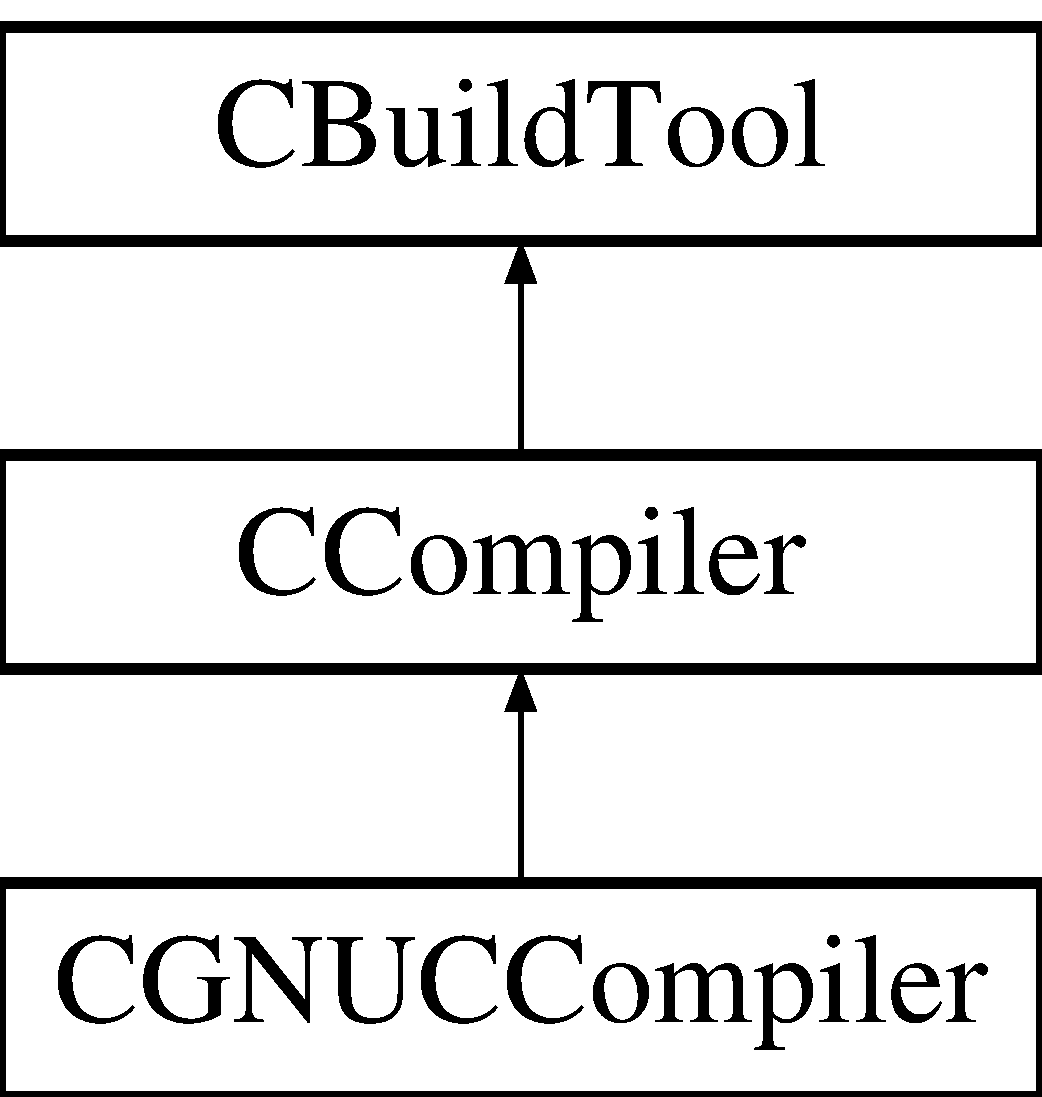
\includegraphics[height=3.000000cm]{db/d59/classCGNUCCompiler}
\end{center}
\end{figure}
\subsection*{Public Member Functions}
\begin{DoxyCompactItemize}
\item 
virtual \hyperlink{classCIncludeSearchFilter}{C\-Include\-Search\-Filter} $\ast$ \hyperlink{classCGNUCCompiler_a1dc37484a88684465d9bbfed8ee335e2}{Include\-Search\-Filter} (void) const 
\item 
virtual \hyperlink{classCGNUCCompiler}{C\-G\-N\-U\-C\-Compiler} $\ast$ \hyperlink{classCGNUCCompiler_ae69827132a9bc1170f2073bf4ded88bc}{Create\-Instance} (void)
\item 
virtual void \hyperlink{classCGNUCCompiler_a56fec9a27346838f33b3c444e90021f7}{Reset} (const \hyperlink{classCPlatform_a2fb735c63c53052f79629e338bb0f535}{C\-Platform\-::\-O\-S\-\_\-\-Type} O\-S)
\item 
\hyperlink{classCGNUCCompiler_a8f773f774ca44bc7cd0d6ef9e1e71211}{C\-G\-N\-U\-C\-Compiler} (void)
\end{DoxyCompactItemize}
\subsection*{Private Attributes}
\begin{DoxyCompactItemize}
\item 
\hyperlink{classCCppIncludeSearchFilter}{C\-Cpp\-Include\-Search\-Filter} \hyperlink{classCGNUCCompiler_ab89fb7c6abd00a9462fcd8334e4aab0a}{m\-\_\-\-Include\-Search\-Filter}
\end{DoxyCompactItemize}
\subsection*{Additional Inherited Members}


\subsection{Constructor \& Destructor Documentation}
\hypertarget{classCGNUCCompiler_a8f773f774ca44bc7cd0d6ef9e1e71211}{\index{C\-G\-N\-U\-C\-Compiler@{C\-G\-N\-U\-C\-Compiler}!C\-G\-N\-U\-C\-Compiler@{C\-G\-N\-U\-C\-Compiler}}
\index{C\-G\-N\-U\-C\-Compiler@{C\-G\-N\-U\-C\-Compiler}!CGNUCCompiler@{C\-G\-N\-U\-C\-Compiler}}
\subsubsection[{C\-G\-N\-U\-C\-Compiler}]{\setlength{\rightskip}{0pt plus 5cm}C\-G\-N\-U\-C\-Compiler\-::\-C\-G\-N\-U\-C\-Compiler (
\begin{DoxyParamCaption}
\item[{void}]{}
\end{DoxyParamCaption}
)}}\label{classCGNUCCompiler_a8f773f774ca44bc7cd0d6ef9e1e71211}


\subsection{Member Function Documentation}
\hypertarget{classCGNUCCompiler_ae69827132a9bc1170f2073bf4ded88bc}{\index{C\-G\-N\-U\-C\-Compiler@{C\-G\-N\-U\-C\-Compiler}!Create\-Instance@{Create\-Instance}}
\index{Create\-Instance@{Create\-Instance}!CGNUCCompiler@{C\-G\-N\-U\-C\-Compiler}}
\subsubsection[{Create\-Instance}]{\setlength{\rightskip}{0pt plus 5cm}{\bf C\-G\-N\-U\-C\-Compiler} $\ast$ C\-G\-N\-U\-C\-Compiler\-::\-Create\-Instance (
\begin{DoxyParamCaption}
\item[{void}]{}
\end{DoxyParamCaption}
)\hspace{0.3cm}{\ttfamily [virtual]}}}\label{classCGNUCCompiler_ae69827132a9bc1170f2073bf4ded88bc}


Reimplemented from \hyperlink{classCCompiler_a3d4aaaf69e1ba6070c729fd042d90012}{C\-Compiler}.

\hypertarget{classCGNUCCompiler_a1dc37484a88684465d9bbfed8ee335e2}{\index{C\-G\-N\-U\-C\-Compiler@{C\-G\-N\-U\-C\-Compiler}!Include\-Search\-Filter@{Include\-Search\-Filter}}
\index{Include\-Search\-Filter@{Include\-Search\-Filter}!CGNUCCompiler@{C\-G\-N\-U\-C\-Compiler}}
\subsubsection[{Include\-Search\-Filter}]{\setlength{\rightskip}{0pt plus 5cm}{\bf C\-Include\-Search\-Filter} $\ast$ C\-G\-N\-U\-C\-Compiler\-::\-Include\-Search\-Filter (
\begin{DoxyParamCaption}
\item[{void}]{}
\end{DoxyParamCaption}
) const\hspace{0.3cm}{\ttfamily [virtual]}}}\label{classCGNUCCompiler_a1dc37484a88684465d9bbfed8ee335e2}


Reimplemented from \hyperlink{classCCompiler_a1dc477f47e953ddd4c653f3ba85c5468}{C\-Compiler}.

\hypertarget{classCGNUCCompiler_a56fec9a27346838f33b3c444e90021f7}{\index{C\-G\-N\-U\-C\-Compiler@{C\-G\-N\-U\-C\-Compiler}!Reset@{Reset}}
\index{Reset@{Reset}!CGNUCCompiler@{C\-G\-N\-U\-C\-Compiler}}
\subsubsection[{Reset}]{\setlength{\rightskip}{0pt plus 5cm}void C\-G\-N\-U\-C\-Compiler\-::\-Reset (
\begin{DoxyParamCaption}
\item[{const {\bf C\-Platform\-::\-O\-S\-\_\-\-Type}}]{O\-S}
\end{DoxyParamCaption}
)\hspace{0.3cm}{\ttfamily [virtual]}}}\label{classCGNUCCompiler_a56fec9a27346838f33b3c444e90021f7}


Reimplemented from \hyperlink{classCBuildTool_abea21a0e61ab2177effdff5aaa169585}{C\-Build\-Tool}.



\subsection{Member Data Documentation}
\hypertarget{classCGNUCCompiler_ab89fb7c6abd00a9462fcd8334e4aab0a}{\index{C\-G\-N\-U\-C\-Compiler@{C\-G\-N\-U\-C\-Compiler}!m\-\_\-\-Include\-Search\-Filter@{m\-\_\-\-Include\-Search\-Filter}}
\index{m\-\_\-\-Include\-Search\-Filter@{m\-\_\-\-Include\-Search\-Filter}!CGNUCCompiler@{C\-G\-N\-U\-C\-Compiler}}
\subsubsection[{m\-\_\-\-Include\-Search\-Filter}]{\setlength{\rightskip}{0pt plus 5cm}{\bf C\-Cpp\-Include\-Search\-Filter} C\-G\-N\-U\-C\-Compiler\-::m\-\_\-\-Include\-Search\-Filter\hspace{0.3cm}{\ttfamily [private]}}}\label{classCGNUCCompiler_ab89fb7c6abd00a9462fcd8334e4aab0a}


The documentation for this class was generated from the following files\-:\begin{DoxyCompactItemize}
\item 
src/\hyperlink{buildtools_8h}{buildtools.\-h}\item 
src/\hyperlink{buildtools_8cpp}{buildtools.\-cpp}\end{DoxyCompactItemize}

\hypertarget{classCGNUCppCompiler}{\section{C\-G\-N\-U\-Cpp\-Compiler Class Reference}
\label{classCGNUCppCompiler}\index{C\-G\-N\-U\-Cpp\-Compiler@{C\-G\-N\-U\-Cpp\-Compiler}}
}


{\ttfamily \#include $<$buildtools.\-h$>$}

Inheritance diagram for C\-G\-N\-U\-Cpp\-Compiler\-:\begin{figure}[H]
\begin{center}
\leavevmode
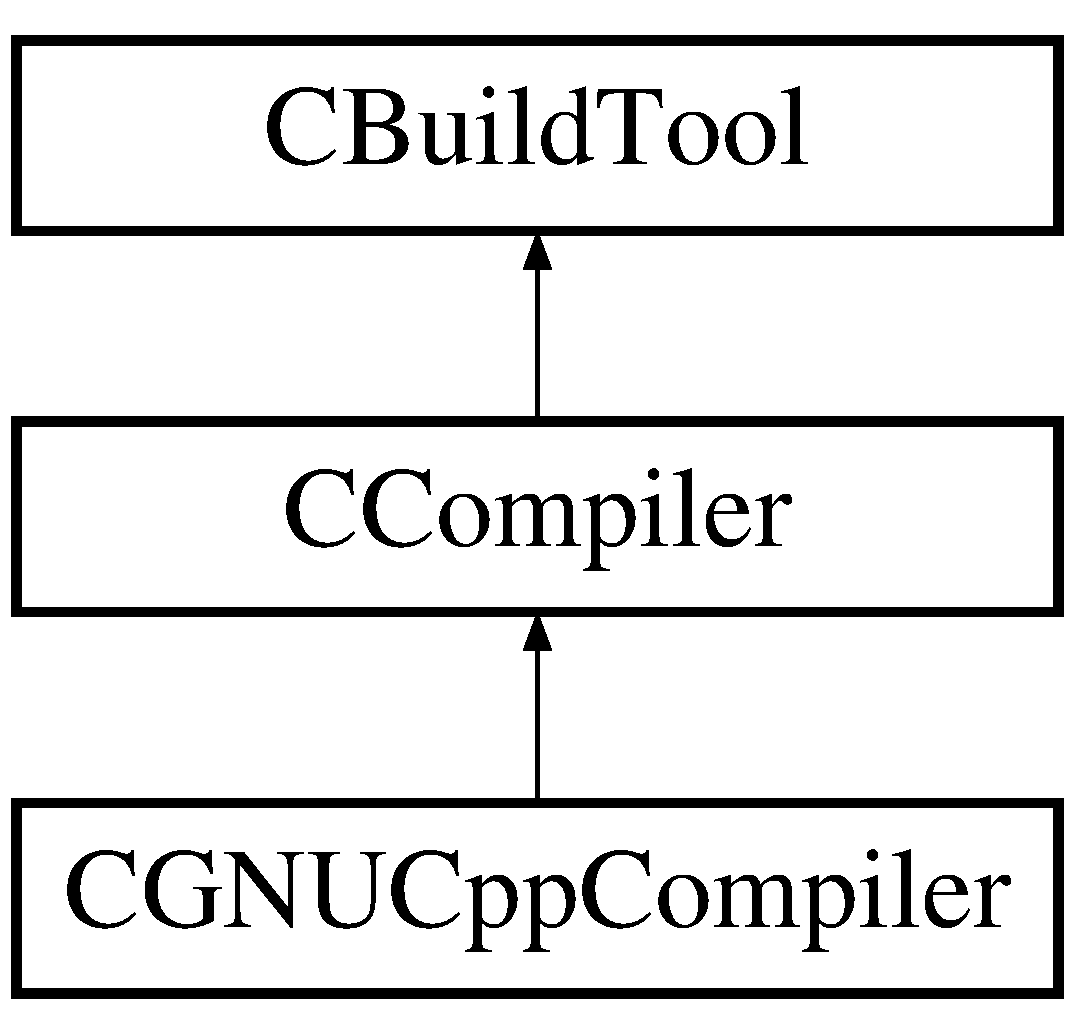
\includegraphics[height=3.000000cm]{d3/d68/classCGNUCppCompiler}
\end{center}
\end{figure}
\subsection*{Public Member Functions}
\begin{DoxyCompactItemize}
\item 
virtual \hyperlink{classCIncludeSearchFilter}{C\-Include\-Search\-Filter} $\ast$ \hyperlink{classCGNUCppCompiler_a70e0a0d27cded35b66807d8e2804ade8}{Include\-Search\-Filter} (void) const 
\item 
virtual \hyperlink{classCGNUCppCompiler}{C\-G\-N\-U\-Cpp\-Compiler} $\ast$ \hyperlink{classCGNUCppCompiler_a0e6856b3906b6b32951f9796fba16316}{Create\-Instance} (void)
\item 
virtual void \hyperlink{classCGNUCppCompiler_ae44ff252152bc51ef1855cc863cb007b}{Reset} (const \hyperlink{classCPlatform_a2fb735c63c53052f79629e338bb0f535}{C\-Platform\-::\-O\-S\-\_\-\-Type} O\-S)
\item 
\hyperlink{classCGNUCppCompiler_a46be2f17939ca4705604ec65b6d3e16d}{C\-G\-N\-U\-Cpp\-Compiler} (void)
\end{DoxyCompactItemize}
\subsection*{Private Attributes}
\begin{DoxyCompactItemize}
\item 
\hyperlink{classCCppIncludeSearchFilter}{C\-Cpp\-Include\-Search\-Filter} \hyperlink{classCGNUCppCompiler_a51684849a7c0aabaa0c780eb06908fb4}{m\-\_\-\-Include\-Search\-Filter}
\end{DoxyCompactItemize}
\subsection*{Additional Inherited Members}


\subsection{Constructor \& Destructor Documentation}
\hypertarget{classCGNUCppCompiler_a46be2f17939ca4705604ec65b6d3e16d}{\index{C\-G\-N\-U\-Cpp\-Compiler@{C\-G\-N\-U\-Cpp\-Compiler}!C\-G\-N\-U\-Cpp\-Compiler@{C\-G\-N\-U\-Cpp\-Compiler}}
\index{C\-G\-N\-U\-Cpp\-Compiler@{C\-G\-N\-U\-Cpp\-Compiler}!CGNUCppCompiler@{C\-G\-N\-U\-Cpp\-Compiler}}
\subsubsection[{C\-G\-N\-U\-Cpp\-Compiler}]{\setlength{\rightskip}{0pt plus 5cm}C\-G\-N\-U\-Cpp\-Compiler\-::\-C\-G\-N\-U\-Cpp\-Compiler (
\begin{DoxyParamCaption}
\item[{void}]{}
\end{DoxyParamCaption}
)}}\label{classCGNUCppCompiler_a46be2f17939ca4705604ec65b6d3e16d}


\subsection{Member Function Documentation}
\hypertarget{classCGNUCppCompiler_a0e6856b3906b6b32951f9796fba16316}{\index{C\-G\-N\-U\-Cpp\-Compiler@{C\-G\-N\-U\-Cpp\-Compiler}!Create\-Instance@{Create\-Instance}}
\index{Create\-Instance@{Create\-Instance}!CGNUCppCompiler@{C\-G\-N\-U\-Cpp\-Compiler}}
\subsubsection[{Create\-Instance}]{\setlength{\rightskip}{0pt plus 5cm}{\bf C\-G\-N\-U\-Cpp\-Compiler} $\ast$ C\-G\-N\-U\-Cpp\-Compiler\-::\-Create\-Instance (
\begin{DoxyParamCaption}
\item[{void}]{}
\end{DoxyParamCaption}
)\hspace{0.3cm}{\ttfamily [virtual]}}}\label{classCGNUCppCompiler_a0e6856b3906b6b32951f9796fba16316}


Reimplemented from \hyperlink{classCCompiler_a3d4aaaf69e1ba6070c729fd042d90012}{C\-Compiler}.

\hypertarget{classCGNUCppCompiler_a70e0a0d27cded35b66807d8e2804ade8}{\index{C\-G\-N\-U\-Cpp\-Compiler@{C\-G\-N\-U\-Cpp\-Compiler}!Include\-Search\-Filter@{Include\-Search\-Filter}}
\index{Include\-Search\-Filter@{Include\-Search\-Filter}!CGNUCppCompiler@{C\-G\-N\-U\-Cpp\-Compiler}}
\subsubsection[{Include\-Search\-Filter}]{\setlength{\rightskip}{0pt plus 5cm}{\bf C\-Include\-Search\-Filter} $\ast$ C\-G\-N\-U\-Cpp\-Compiler\-::\-Include\-Search\-Filter (
\begin{DoxyParamCaption}
\item[{void}]{}
\end{DoxyParamCaption}
) const\hspace{0.3cm}{\ttfamily [virtual]}}}\label{classCGNUCppCompiler_a70e0a0d27cded35b66807d8e2804ade8}


Reimplemented from \hyperlink{classCCompiler_a1dc477f47e953ddd4c653f3ba85c5468}{C\-Compiler}.

\hypertarget{classCGNUCppCompiler_ae44ff252152bc51ef1855cc863cb007b}{\index{C\-G\-N\-U\-Cpp\-Compiler@{C\-G\-N\-U\-Cpp\-Compiler}!Reset@{Reset}}
\index{Reset@{Reset}!CGNUCppCompiler@{C\-G\-N\-U\-Cpp\-Compiler}}
\subsubsection[{Reset}]{\setlength{\rightskip}{0pt plus 5cm}void C\-G\-N\-U\-Cpp\-Compiler\-::\-Reset (
\begin{DoxyParamCaption}
\item[{const {\bf C\-Platform\-::\-O\-S\-\_\-\-Type}}]{O\-S}
\end{DoxyParamCaption}
)\hspace{0.3cm}{\ttfamily [virtual]}}}\label{classCGNUCppCompiler_ae44ff252152bc51ef1855cc863cb007b}


Reimplemented from \hyperlink{classCBuildTool_abea21a0e61ab2177effdff5aaa169585}{C\-Build\-Tool}.



\subsection{Member Data Documentation}
\hypertarget{classCGNUCppCompiler_a51684849a7c0aabaa0c780eb06908fb4}{\index{C\-G\-N\-U\-Cpp\-Compiler@{C\-G\-N\-U\-Cpp\-Compiler}!m\-\_\-\-Include\-Search\-Filter@{m\-\_\-\-Include\-Search\-Filter}}
\index{m\-\_\-\-Include\-Search\-Filter@{m\-\_\-\-Include\-Search\-Filter}!CGNUCppCompiler@{C\-G\-N\-U\-Cpp\-Compiler}}
\subsubsection[{m\-\_\-\-Include\-Search\-Filter}]{\setlength{\rightskip}{0pt plus 5cm}{\bf C\-Cpp\-Include\-Search\-Filter} C\-G\-N\-U\-Cpp\-Compiler\-::m\-\_\-\-Include\-Search\-Filter\hspace{0.3cm}{\ttfamily [private]}}}\label{classCGNUCppCompiler_a51684849a7c0aabaa0c780eb06908fb4}


The documentation for this class was generated from the following files\-:\begin{DoxyCompactItemize}
\item 
src/\hyperlink{buildtools_8h}{buildtools.\-h}\item 
src/\hyperlink{buildtools_8cpp}{buildtools.\-cpp}\end{DoxyCompactItemize}

\hypertarget{classCGNUDynamicLinker}{\section{C\-G\-N\-U\-Dynamic\-Linker Class Reference}
\label{classCGNUDynamicLinker}\index{C\-G\-N\-U\-Dynamic\-Linker@{C\-G\-N\-U\-Dynamic\-Linker}}
}


{\ttfamily \#include $<$buildtools.\-h$>$}

Inheritance diagram for C\-G\-N\-U\-Dynamic\-Linker\-:\begin{figure}[H]
\begin{center}
\leavevmode
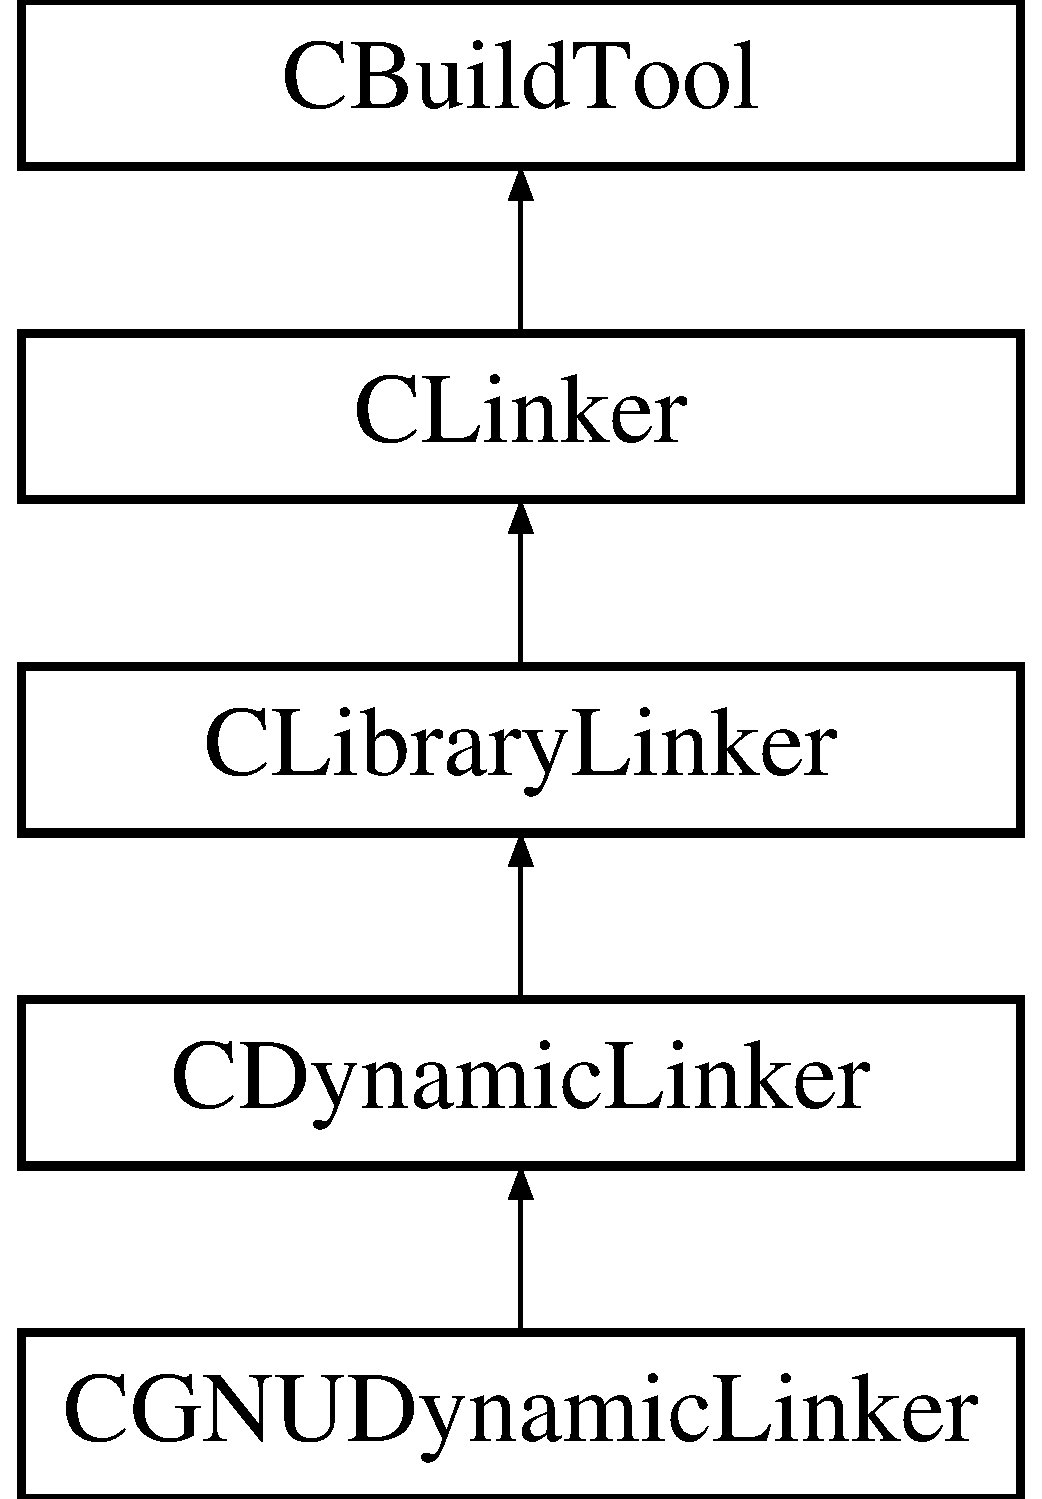
\includegraphics[height=5.000000cm]{d5/dc1/classCGNUDynamicLinker}
\end{center}
\end{figure}
\subsection*{Public Member Functions}
\begin{DoxyCompactItemize}
\item 
virtual \hyperlink{classCGNUDynamicLinker}{C\-G\-N\-U\-Dynamic\-Linker} $\ast$ \hyperlink{classCGNUDynamicLinker_addcaa2506e1f804b4737cb564a899f6c}{Create\-Instance} (void)
\item 
virtual void \hyperlink{classCGNUDynamicLinker_ae156df1627238831556bd40597694d7e}{Reset} (const \hyperlink{classCPlatform_a2fb735c63c53052f79629e338bb0f535}{C\-Platform\-::\-O\-S\-\_\-\-Type} O\-S)
\item 
\hyperlink{classCGNUDynamicLinker_a85f3a72d68faaff0a2d23475f044dad6}{C\-G\-N\-U\-Dynamic\-Linker} (void)
\end{DoxyCompactItemize}
\subsection*{Additional Inherited Members}


\subsection{Constructor \& Destructor Documentation}
\hypertarget{classCGNUDynamicLinker_a85f3a72d68faaff0a2d23475f044dad6}{\index{C\-G\-N\-U\-Dynamic\-Linker@{C\-G\-N\-U\-Dynamic\-Linker}!C\-G\-N\-U\-Dynamic\-Linker@{C\-G\-N\-U\-Dynamic\-Linker}}
\index{C\-G\-N\-U\-Dynamic\-Linker@{C\-G\-N\-U\-Dynamic\-Linker}!CGNUDynamicLinker@{C\-G\-N\-U\-Dynamic\-Linker}}
\subsubsection[{C\-G\-N\-U\-Dynamic\-Linker}]{\setlength{\rightskip}{0pt plus 5cm}C\-G\-N\-U\-Dynamic\-Linker\-::\-C\-G\-N\-U\-Dynamic\-Linker (
\begin{DoxyParamCaption}
\item[{void}]{}
\end{DoxyParamCaption}
)}}\label{classCGNUDynamicLinker_a85f3a72d68faaff0a2d23475f044dad6}


\subsection{Member Function Documentation}
\hypertarget{classCGNUDynamicLinker_addcaa2506e1f804b4737cb564a899f6c}{\index{C\-G\-N\-U\-Dynamic\-Linker@{C\-G\-N\-U\-Dynamic\-Linker}!Create\-Instance@{Create\-Instance}}
\index{Create\-Instance@{Create\-Instance}!CGNUDynamicLinker@{C\-G\-N\-U\-Dynamic\-Linker}}
\subsubsection[{Create\-Instance}]{\setlength{\rightskip}{0pt plus 5cm}{\bf C\-G\-N\-U\-Dynamic\-Linker} $\ast$ C\-G\-N\-U\-Dynamic\-Linker\-::\-Create\-Instance (
\begin{DoxyParamCaption}
\item[{void}]{}
\end{DoxyParamCaption}
)\hspace{0.3cm}{\ttfamily [virtual]}}}\label{classCGNUDynamicLinker_addcaa2506e1f804b4737cb564a899f6c}


Reimplemented from \hyperlink{classCDynamicLinker_ac71406ca5c6e8e991a6418a6307d274c}{C\-Dynamic\-Linker}.

\hypertarget{classCGNUDynamicLinker_ae156df1627238831556bd40597694d7e}{\index{C\-G\-N\-U\-Dynamic\-Linker@{C\-G\-N\-U\-Dynamic\-Linker}!Reset@{Reset}}
\index{Reset@{Reset}!CGNUDynamicLinker@{C\-G\-N\-U\-Dynamic\-Linker}}
\subsubsection[{Reset}]{\setlength{\rightskip}{0pt plus 5cm}void C\-G\-N\-U\-Dynamic\-Linker\-::\-Reset (
\begin{DoxyParamCaption}
\item[{const {\bf C\-Platform\-::\-O\-S\-\_\-\-Type}}]{O\-S}
\end{DoxyParamCaption}
)\hspace{0.3cm}{\ttfamily [virtual]}}}\label{classCGNUDynamicLinker_ae156df1627238831556bd40597694d7e}


Reimplemented from \hyperlink{classCDynamicLinker_a437d46ee65b3585e7be9d15d40c26820}{C\-Dynamic\-Linker}.



The documentation for this class was generated from the following files\-:\begin{DoxyCompactItemize}
\item 
src/\hyperlink{buildtools_8h}{buildtools.\-h}\item 
src/\hyperlink{buildtools_8cpp}{buildtools.\-cpp}\end{DoxyCompactItemize}

\hypertarget{classCGNUExecutableLinker}{\section{C\-G\-N\-U\-Executable\-Linker Class Reference}
\label{classCGNUExecutableLinker}\index{C\-G\-N\-U\-Executable\-Linker@{C\-G\-N\-U\-Executable\-Linker}}
}


{\ttfamily \#include $<$buildtools.\-h$>$}

Inheritance diagram for C\-G\-N\-U\-Executable\-Linker\-:\begin{figure}[H]
\begin{center}
\leavevmode
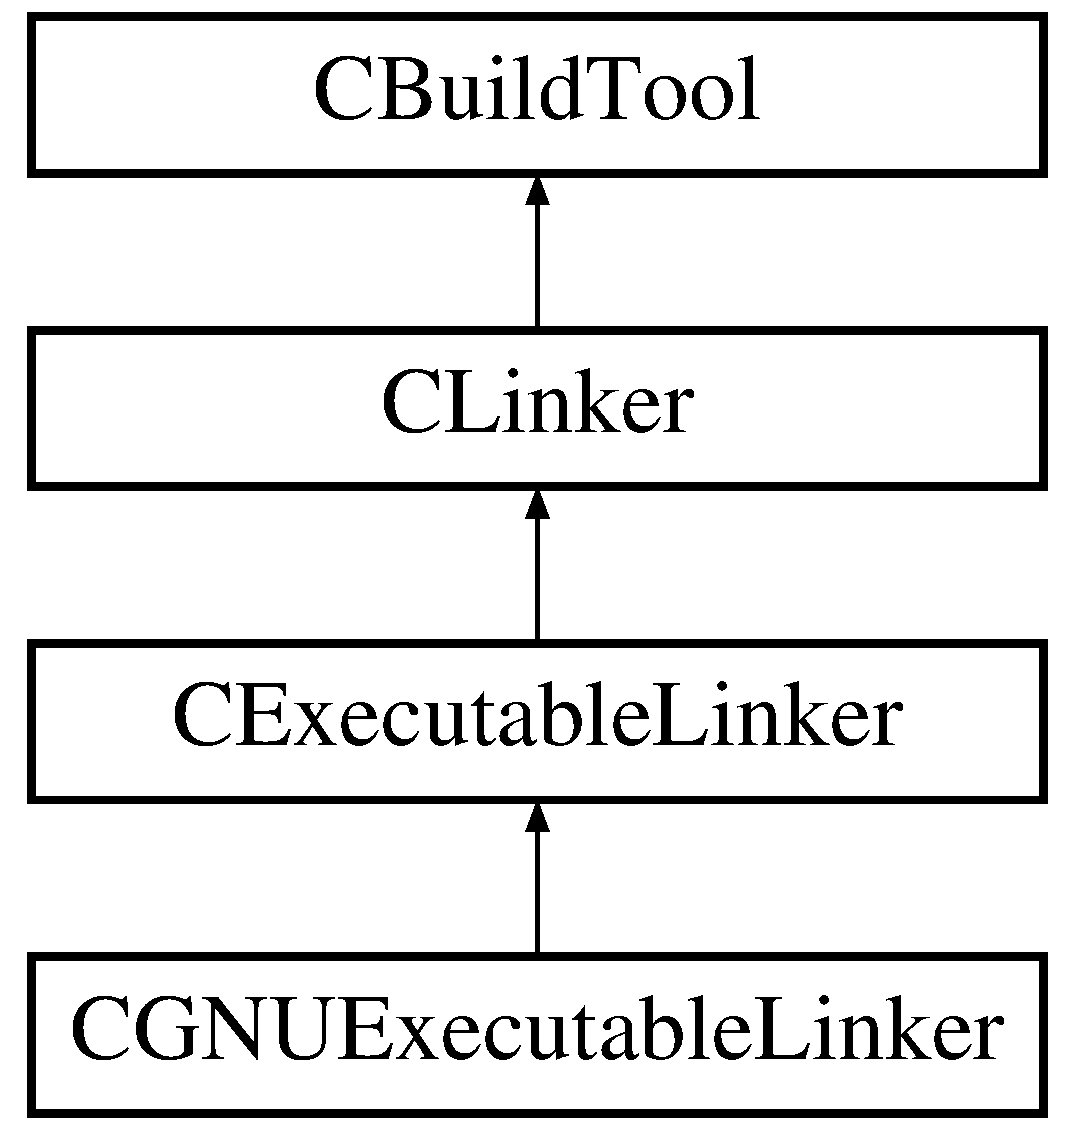
\includegraphics[height=4.000000cm]{df/d25/classCGNUExecutableLinker}
\end{center}
\end{figure}
\subsection*{Public Member Functions}
\begin{DoxyCompactItemize}
\item 
virtual \hyperlink{classCGNUExecutableLinker}{C\-G\-N\-U\-Executable\-Linker} $\ast$ \hyperlink{classCGNUExecutableLinker_a96d5c82ab5c7c26e7e9ef1542c815e94}{Create\-Instance} (void)
\item 
virtual void \hyperlink{classCGNUExecutableLinker_a79d1592b592c3b48d7e1683cdb516d85}{Reset} (const \hyperlink{classCPlatform_a2fb735c63c53052f79629e338bb0f535}{C\-Platform\-::\-O\-S\-\_\-\-Type} O\-S)
\item 
\hyperlink{classCGNUExecutableLinker_a6e86ba5d35ac83ecbd0342e9565af695}{C\-G\-N\-U\-Executable\-Linker} (void)
\end{DoxyCompactItemize}
\subsection*{Additional Inherited Members}


\subsection{Constructor \& Destructor Documentation}
\hypertarget{classCGNUExecutableLinker_a6e86ba5d35ac83ecbd0342e9565af695}{\index{C\-G\-N\-U\-Executable\-Linker@{C\-G\-N\-U\-Executable\-Linker}!C\-G\-N\-U\-Executable\-Linker@{C\-G\-N\-U\-Executable\-Linker}}
\index{C\-G\-N\-U\-Executable\-Linker@{C\-G\-N\-U\-Executable\-Linker}!CGNUExecutableLinker@{C\-G\-N\-U\-Executable\-Linker}}
\subsubsection[{C\-G\-N\-U\-Executable\-Linker}]{\setlength{\rightskip}{0pt plus 5cm}C\-G\-N\-U\-Executable\-Linker\-::\-C\-G\-N\-U\-Executable\-Linker (
\begin{DoxyParamCaption}
\item[{void}]{}
\end{DoxyParamCaption}
)}}\label{classCGNUExecutableLinker_a6e86ba5d35ac83ecbd0342e9565af695}


\subsection{Member Function Documentation}
\hypertarget{classCGNUExecutableLinker_a96d5c82ab5c7c26e7e9ef1542c815e94}{\index{C\-G\-N\-U\-Executable\-Linker@{C\-G\-N\-U\-Executable\-Linker}!Create\-Instance@{Create\-Instance}}
\index{Create\-Instance@{Create\-Instance}!CGNUExecutableLinker@{C\-G\-N\-U\-Executable\-Linker}}
\subsubsection[{Create\-Instance}]{\setlength{\rightskip}{0pt plus 5cm}{\bf C\-G\-N\-U\-Executable\-Linker} $\ast$ C\-G\-N\-U\-Executable\-Linker\-::\-Create\-Instance (
\begin{DoxyParamCaption}
\item[{void}]{}
\end{DoxyParamCaption}
)\hspace{0.3cm}{\ttfamily [virtual]}}}\label{classCGNUExecutableLinker_a96d5c82ab5c7c26e7e9ef1542c815e94}


Reimplemented from \hyperlink{classCExecutableLinker_a457b823b737b0a78285d5ede77df827c}{C\-Executable\-Linker}.

\hypertarget{classCGNUExecutableLinker_a79d1592b592c3b48d7e1683cdb516d85}{\index{C\-G\-N\-U\-Executable\-Linker@{C\-G\-N\-U\-Executable\-Linker}!Reset@{Reset}}
\index{Reset@{Reset}!CGNUExecutableLinker@{C\-G\-N\-U\-Executable\-Linker}}
\subsubsection[{Reset}]{\setlength{\rightskip}{0pt plus 5cm}void C\-G\-N\-U\-Executable\-Linker\-::\-Reset (
\begin{DoxyParamCaption}
\item[{const {\bf C\-Platform\-::\-O\-S\-\_\-\-Type}}]{O\-S}
\end{DoxyParamCaption}
)\hspace{0.3cm}{\ttfamily [virtual]}}}\label{classCGNUExecutableLinker_a79d1592b592c3b48d7e1683cdb516d85}


Reimplemented from \hyperlink{classCBuildTool_abea21a0e61ab2177effdff5aaa169585}{C\-Build\-Tool}.



The documentation for this class was generated from the following files\-:\begin{DoxyCompactItemize}
\item 
src/\hyperlink{buildtools_8h}{buildtools.\-h}\item 
src/\hyperlink{buildtools_8cpp}{buildtools.\-cpp}\end{DoxyCompactItemize}

\hypertarget{classCGNUFortran77Compiler}{\section{C\-G\-N\-U\-Fortran77\-Compiler Class Reference}
\label{classCGNUFortran77Compiler}\index{C\-G\-N\-U\-Fortran77\-Compiler@{C\-G\-N\-U\-Fortran77\-Compiler}}
}


{\ttfamily \#include $<$buildtools.\-h$>$}

Inheritance diagram for C\-G\-N\-U\-Fortran77\-Compiler\-:\begin{figure}[H]
\begin{center}
\leavevmode
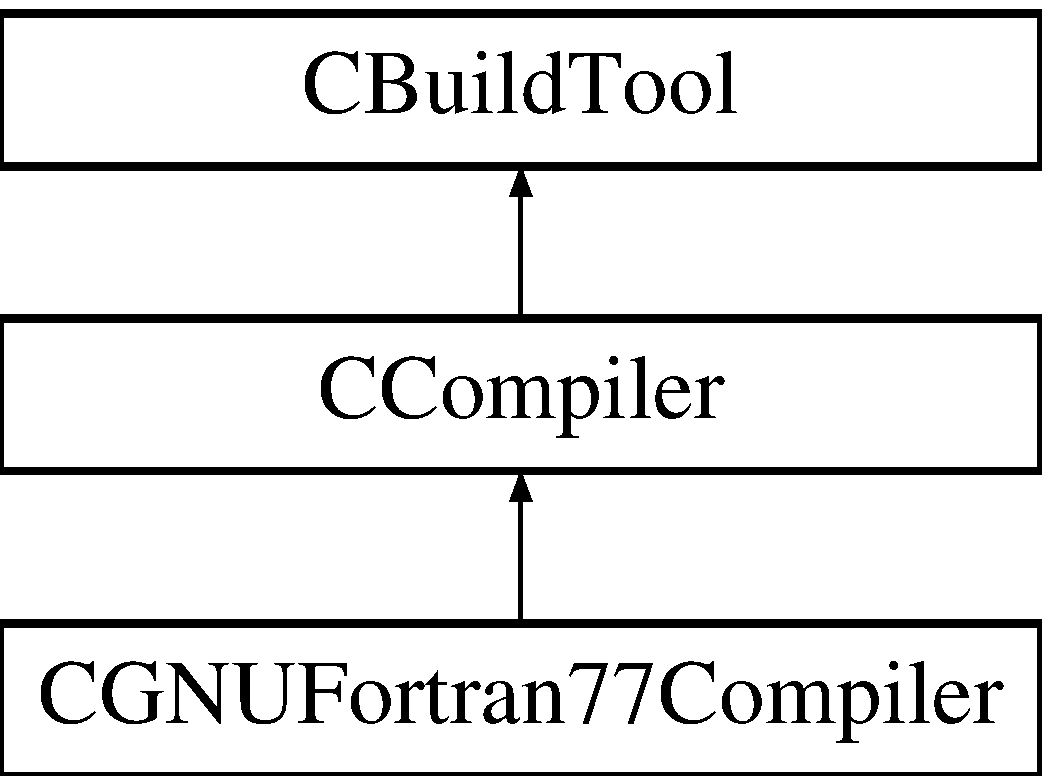
\includegraphics[height=3.000000cm]{dc/dbd/classCGNUFortran77Compiler}
\end{center}
\end{figure}
\subsection*{Public Member Functions}
\begin{DoxyCompactItemize}
\item 
virtual \hyperlink{classCGNUFortran77Compiler}{C\-G\-N\-U\-Fortran77\-Compiler} $\ast$ \hyperlink{classCGNUFortran77Compiler_ac9303b9366e63a08983cabcdfcb5cf06}{Create\-Instance} (void)
\item 
virtual void \hyperlink{classCGNUFortran77Compiler_a67867de4d567f8afc4758083b29be23a}{Reset} (const \hyperlink{classCPlatform_a2fb735c63c53052f79629e338bb0f535}{C\-Platform\-::\-O\-S\-\_\-\-Type} O\-S)
\item 
\hyperlink{classCGNUFortran77Compiler_a4009a7af93f39dccf8209b91a751d5b2}{C\-G\-N\-U\-Fortran77\-Compiler} (void)
\end{DoxyCompactItemize}
\subsection*{Additional Inherited Members}


\subsection{Constructor \& Destructor Documentation}
\hypertarget{classCGNUFortran77Compiler_a4009a7af93f39dccf8209b91a751d5b2}{\index{C\-G\-N\-U\-Fortran77\-Compiler@{C\-G\-N\-U\-Fortran77\-Compiler}!C\-G\-N\-U\-Fortran77\-Compiler@{C\-G\-N\-U\-Fortran77\-Compiler}}
\index{C\-G\-N\-U\-Fortran77\-Compiler@{C\-G\-N\-U\-Fortran77\-Compiler}!CGNUFortran77Compiler@{C\-G\-N\-U\-Fortran77\-Compiler}}
\subsubsection[{C\-G\-N\-U\-Fortran77\-Compiler}]{\setlength{\rightskip}{0pt plus 5cm}C\-G\-N\-U\-Fortran77\-Compiler\-::\-C\-G\-N\-U\-Fortran77\-Compiler (
\begin{DoxyParamCaption}
\item[{void}]{}
\end{DoxyParamCaption}
)}}\label{classCGNUFortran77Compiler_a4009a7af93f39dccf8209b91a751d5b2}


\subsection{Member Function Documentation}
\hypertarget{classCGNUFortran77Compiler_ac9303b9366e63a08983cabcdfcb5cf06}{\index{C\-G\-N\-U\-Fortran77\-Compiler@{C\-G\-N\-U\-Fortran77\-Compiler}!Create\-Instance@{Create\-Instance}}
\index{Create\-Instance@{Create\-Instance}!CGNUFortran77Compiler@{C\-G\-N\-U\-Fortran77\-Compiler}}
\subsubsection[{Create\-Instance}]{\setlength{\rightskip}{0pt plus 5cm}{\bf C\-G\-N\-U\-Fortran77\-Compiler} $\ast$ C\-G\-N\-U\-Fortran77\-Compiler\-::\-Create\-Instance (
\begin{DoxyParamCaption}
\item[{void}]{}
\end{DoxyParamCaption}
)\hspace{0.3cm}{\ttfamily [virtual]}}}\label{classCGNUFortran77Compiler_ac9303b9366e63a08983cabcdfcb5cf06}


Reimplemented from \hyperlink{classCCompiler_a3d4aaaf69e1ba6070c729fd042d90012}{C\-Compiler}.

\hypertarget{classCGNUFortran77Compiler_a67867de4d567f8afc4758083b29be23a}{\index{C\-G\-N\-U\-Fortran77\-Compiler@{C\-G\-N\-U\-Fortran77\-Compiler}!Reset@{Reset}}
\index{Reset@{Reset}!CGNUFortran77Compiler@{C\-G\-N\-U\-Fortran77\-Compiler}}
\subsubsection[{Reset}]{\setlength{\rightskip}{0pt plus 5cm}void C\-G\-N\-U\-Fortran77\-Compiler\-::\-Reset (
\begin{DoxyParamCaption}
\item[{const {\bf C\-Platform\-::\-O\-S\-\_\-\-Type}}]{O\-S}
\end{DoxyParamCaption}
)\hspace{0.3cm}{\ttfamily [virtual]}}}\label{classCGNUFortran77Compiler_a67867de4d567f8afc4758083b29be23a}


Reimplemented from \hyperlink{classCBuildTool_abea21a0e61ab2177effdff5aaa169585}{C\-Build\-Tool}.



The documentation for this class was generated from the following files\-:\begin{DoxyCompactItemize}
\item 
src/\hyperlink{buildtools_8h}{buildtools.\-h}\item 
src/\hyperlink{buildtools_8cpp}{buildtools.\-cpp}\end{DoxyCompactItemize}

\hypertarget{classCGNUFortran90Compiler}{\section{C\-G\-N\-U\-Fortran90\-Compiler Class Reference}
\label{classCGNUFortran90Compiler}\index{C\-G\-N\-U\-Fortran90\-Compiler@{C\-G\-N\-U\-Fortran90\-Compiler}}
}


{\ttfamily \#include $<$buildtools.\-h$>$}

Inheritance diagram for C\-G\-N\-U\-Fortran90\-Compiler\-:\begin{figure}[H]
\begin{center}
\leavevmode
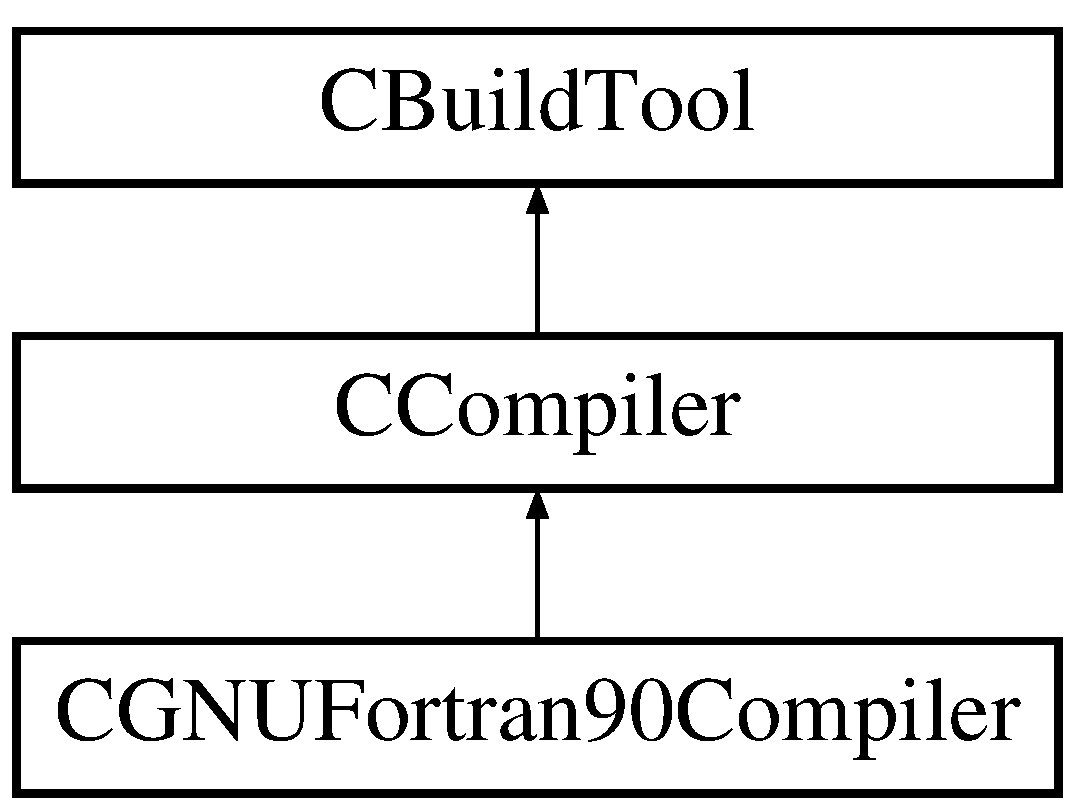
\includegraphics[height=3.000000cm]{dc/d5e/classCGNUFortran90Compiler}
\end{center}
\end{figure}
\subsection*{Public Member Functions}
\begin{DoxyCompactItemize}
\item 
virtual \hyperlink{classCGNUFortran90Compiler}{C\-G\-N\-U\-Fortran90\-Compiler} $\ast$ \hyperlink{classCGNUFortran90Compiler_a40bbc9c4d1417331e65990ed6f402d24}{Create\-Instance} (void)
\item 
virtual void \hyperlink{classCGNUFortran90Compiler_a6ab744c56fb1f147587fee587d15b652}{Reset} (const \hyperlink{classCPlatform_a2fb735c63c53052f79629e338bb0f535}{C\-Platform\-::\-O\-S\-\_\-\-Type} O\-S)
\item 
\hyperlink{classCGNUFortran90Compiler_a1ce529c0617dbed63ec3298ae3e7bcd4}{C\-G\-N\-U\-Fortran90\-Compiler} (void)
\end{DoxyCompactItemize}
\subsection*{Additional Inherited Members}


\subsection{Constructor \& Destructor Documentation}
\hypertarget{classCGNUFortran90Compiler_a1ce529c0617dbed63ec3298ae3e7bcd4}{\index{C\-G\-N\-U\-Fortran90\-Compiler@{C\-G\-N\-U\-Fortran90\-Compiler}!C\-G\-N\-U\-Fortran90\-Compiler@{C\-G\-N\-U\-Fortran90\-Compiler}}
\index{C\-G\-N\-U\-Fortran90\-Compiler@{C\-G\-N\-U\-Fortran90\-Compiler}!CGNUFortran90Compiler@{C\-G\-N\-U\-Fortran90\-Compiler}}
\subsubsection[{C\-G\-N\-U\-Fortran90\-Compiler}]{\setlength{\rightskip}{0pt plus 5cm}C\-G\-N\-U\-Fortran90\-Compiler\-::\-C\-G\-N\-U\-Fortran90\-Compiler (
\begin{DoxyParamCaption}
\item[{void}]{}
\end{DoxyParamCaption}
)}}\label{classCGNUFortran90Compiler_a1ce529c0617dbed63ec3298ae3e7bcd4}


\subsection{Member Function Documentation}
\hypertarget{classCGNUFortran90Compiler_a40bbc9c4d1417331e65990ed6f402d24}{\index{C\-G\-N\-U\-Fortran90\-Compiler@{C\-G\-N\-U\-Fortran90\-Compiler}!Create\-Instance@{Create\-Instance}}
\index{Create\-Instance@{Create\-Instance}!CGNUFortran90Compiler@{C\-G\-N\-U\-Fortran90\-Compiler}}
\subsubsection[{Create\-Instance}]{\setlength{\rightskip}{0pt plus 5cm}{\bf C\-G\-N\-U\-Fortran90\-Compiler} $\ast$ C\-G\-N\-U\-Fortran90\-Compiler\-::\-Create\-Instance (
\begin{DoxyParamCaption}
\item[{void}]{}
\end{DoxyParamCaption}
)\hspace{0.3cm}{\ttfamily [virtual]}}}\label{classCGNUFortran90Compiler_a40bbc9c4d1417331e65990ed6f402d24}


Reimplemented from \hyperlink{classCCompiler_a3d4aaaf69e1ba6070c729fd042d90012}{C\-Compiler}.

\hypertarget{classCGNUFortran90Compiler_a6ab744c56fb1f147587fee587d15b652}{\index{C\-G\-N\-U\-Fortran90\-Compiler@{C\-G\-N\-U\-Fortran90\-Compiler}!Reset@{Reset}}
\index{Reset@{Reset}!CGNUFortran90Compiler@{C\-G\-N\-U\-Fortran90\-Compiler}}
\subsubsection[{Reset}]{\setlength{\rightskip}{0pt plus 5cm}void C\-G\-N\-U\-Fortran90\-Compiler\-::\-Reset (
\begin{DoxyParamCaption}
\item[{const {\bf C\-Platform\-::\-O\-S\-\_\-\-Type}}]{O\-S}
\end{DoxyParamCaption}
)\hspace{0.3cm}{\ttfamily [virtual]}}}\label{classCGNUFortran90Compiler_a6ab744c56fb1f147587fee587d15b652}


Reimplemented from \hyperlink{classCBuildTool_abea21a0e61ab2177effdff5aaa169585}{C\-Build\-Tool}.



The documentation for this class was generated from the following files\-:\begin{DoxyCompactItemize}
\item 
src/\hyperlink{buildtools_8h}{buildtools.\-h}\item 
src/\hyperlink{buildtools_8cpp}{buildtools.\-cpp}\end{DoxyCompactItemize}

\hypertarget{classCGNUStaticLinker}{\section{C\-G\-N\-U\-Static\-Linker Class Reference}
\label{classCGNUStaticLinker}\index{C\-G\-N\-U\-Static\-Linker@{C\-G\-N\-U\-Static\-Linker}}
}


{\ttfamily \#include $<$buildtools.\-h$>$}

Inheritance diagram for C\-G\-N\-U\-Static\-Linker\-:\begin{figure}[H]
\begin{center}
\leavevmode
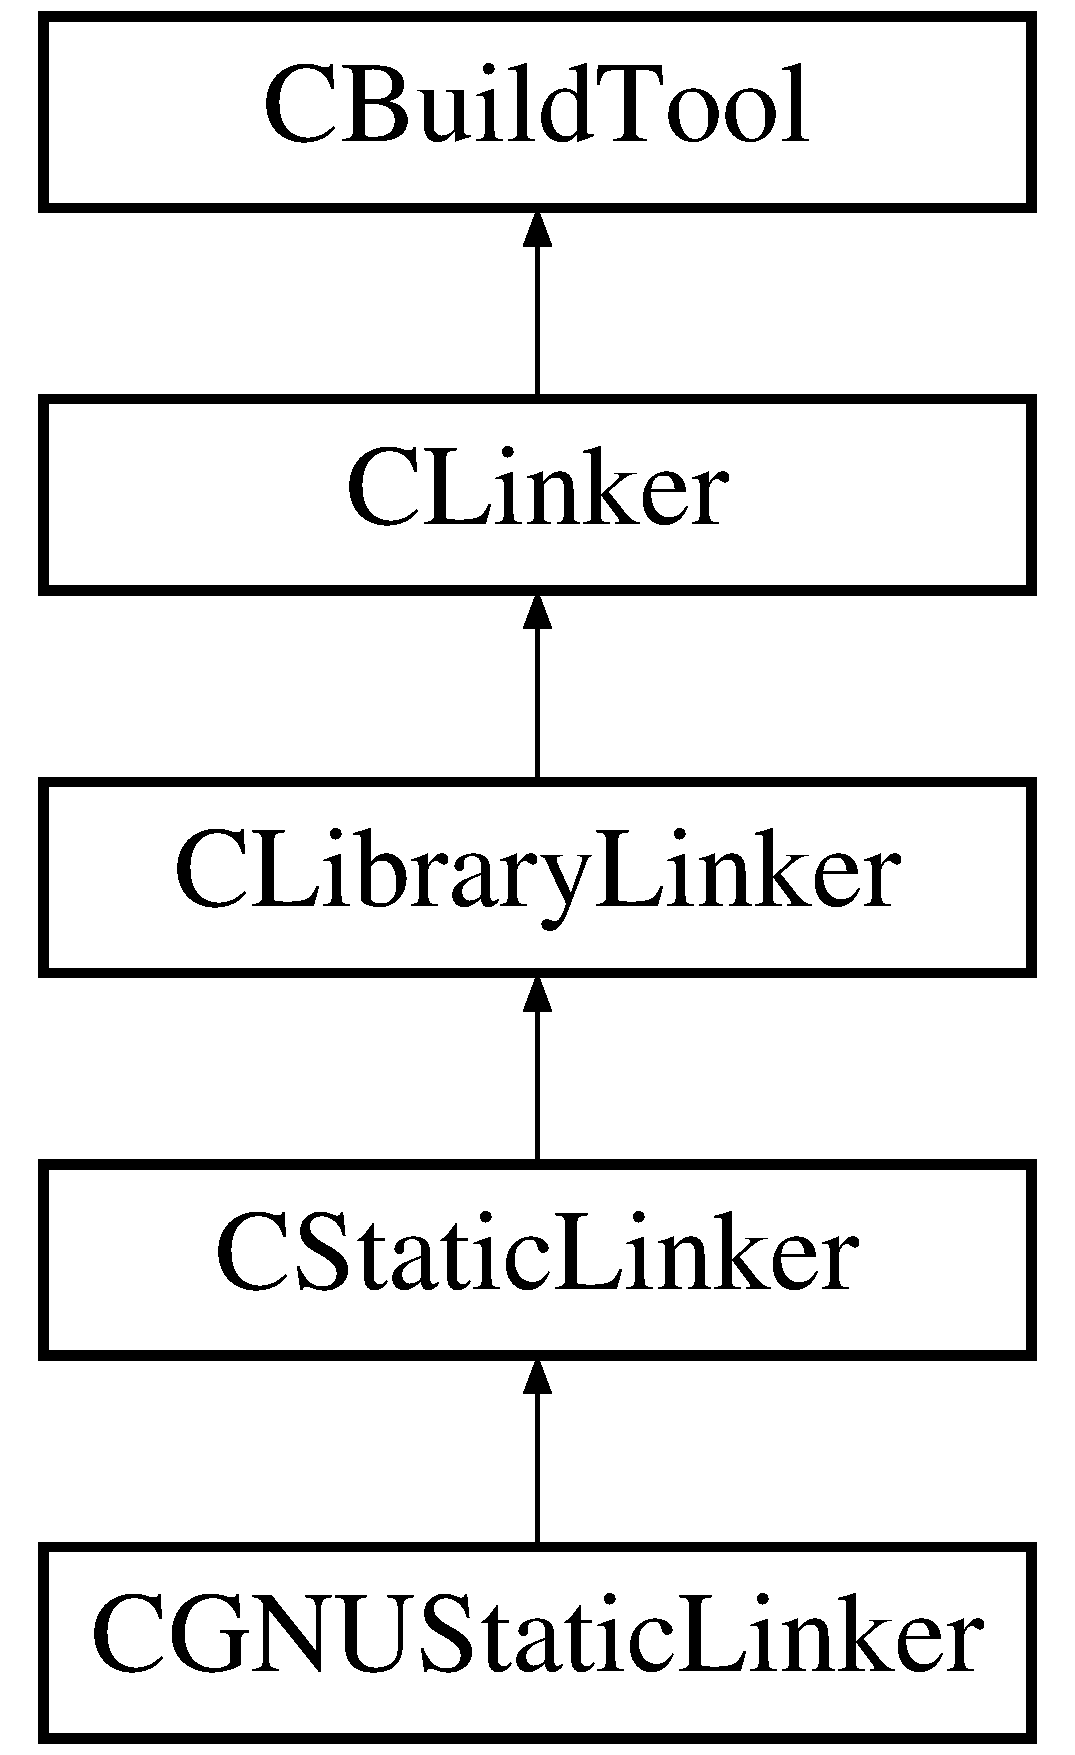
\includegraphics[height=5.000000cm]{dc/d6e/classCGNUStaticLinker}
\end{center}
\end{figure}
\subsection*{Public Member Functions}
\begin{DoxyCompactItemize}
\item 
virtual \hyperlink{classCGNUStaticLinker}{C\-G\-N\-U\-Static\-Linker} $\ast$ \hyperlink{classCGNUStaticLinker_aa2e18f13e37d6c4fe3016d55bc67f746}{Create\-Instance} (void)
\item 
virtual void \hyperlink{classCGNUStaticLinker_a12dca4d9b21cac925906776310521240}{Reset} (const \hyperlink{classCPlatform_a2fb735c63c53052f79629e338bb0f535}{C\-Platform\-::\-O\-S\-\_\-\-Type} O\-S)
\item 
\hyperlink{classCGNUStaticLinker_ad8465b4ad3839735927c5b5c876d08ec}{C\-G\-N\-U\-Static\-Linker} (void)
\end{DoxyCompactItemize}
\subsection*{Additional Inherited Members}


\subsection{Constructor \& Destructor Documentation}
\hypertarget{classCGNUStaticLinker_ad8465b4ad3839735927c5b5c876d08ec}{\index{C\-G\-N\-U\-Static\-Linker@{C\-G\-N\-U\-Static\-Linker}!C\-G\-N\-U\-Static\-Linker@{C\-G\-N\-U\-Static\-Linker}}
\index{C\-G\-N\-U\-Static\-Linker@{C\-G\-N\-U\-Static\-Linker}!CGNUStaticLinker@{C\-G\-N\-U\-Static\-Linker}}
\subsubsection[{C\-G\-N\-U\-Static\-Linker}]{\setlength{\rightskip}{0pt plus 5cm}C\-G\-N\-U\-Static\-Linker\-::\-C\-G\-N\-U\-Static\-Linker (
\begin{DoxyParamCaption}
\item[{void}]{}
\end{DoxyParamCaption}
)}}\label{classCGNUStaticLinker_ad8465b4ad3839735927c5b5c876d08ec}


\subsection{Member Function Documentation}
\hypertarget{classCGNUStaticLinker_aa2e18f13e37d6c4fe3016d55bc67f746}{\index{C\-G\-N\-U\-Static\-Linker@{C\-G\-N\-U\-Static\-Linker}!Create\-Instance@{Create\-Instance}}
\index{Create\-Instance@{Create\-Instance}!CGNUStaticLinker@{C\-G\-N\-U\-Static\-Linker}}
\subsubsection[{Create\-Instance}]{\setlength{\rightskip}{0pt plus 5cm}{\bf C\-G\-N\-U\-Static\-Linker} $\ast$ C\-G\-N\-U\-Static\-Linker\-::\-Create\-Instance (
\begin{DoxyParamCaption}
\item[{void}]{}
\end{DoxyParamCaption}
)\hspace{0.3cm}{\ttfamily [virtual]}}}\label{classCGNUStaticLinker_aa2e18f13e37d6c4fe3016d55bc67f746}


Reimplemented from \hyperlink{classCStaticLinker_a7e626491caa847ef207032ee600625db}{C\-Static\-Linker}.

\hypertarget{classCGNUStaticLinker_a12dca4d9b21cac925906776310521240}{\index{C\-G\-N\-U\-Static\-Linker@{C\-G\-N\-U\-Static\-Linker}!Reset@{Reset}}
\index{Reset@{Reset}!CGNUStaticLinker@{C\-G\-N\-U\-Static\-Linker}}
\subsubsection[{Reset}]{\setlength{\rightskip}{0pt plus 5cm}void C\-G\-N\-U\-Static\-Linker\-::\-Reset (
\begin{DoxyParamCaption}
\item[{const {\bf C\-Platform\-::\-O\-S\-\_\-\-Type}}]{O\-S}
\end{DoxyParamCaption}
)\hspace{0.3cm}{\ttfamily [virtual]}}}\label{classCGNUStaticLinker_a12dca4d9b21cac925906776310521240}


Reimplemented from \hyperlink{classCBuildTool_abea21a0e61ab2177effdff5aaa169585}{C\-Build\-Tool}.



The documentation for this class was generated from the following files\-:\begin{DoxyCompactItemize}
\item 
src/\hyperlink{buildtools_8h}{buildtools.\-h}\item 
src/\hyperlink{buildtools_8cpp}{buildtools.\-cpp}\end{DoxyCompactItemize}

\hypertarget{classCGNUToolChain}{\section{C\-G\-N\-U\-Tool\-Chain Class Reference}
\label{classCGNUToolChain}\index{C\-G\-N\-U\-Tool\-Chain@{C\-G\-N\-U\-Tool\-Chain}}
}


{\ttfamily \#include $<$toolchains.\-h$>$}

Inheritance diagram for C\-G\-N\-U\-Tool\-Chain\-:\begin{figure}[H]
\begin{center}
\leavevmode
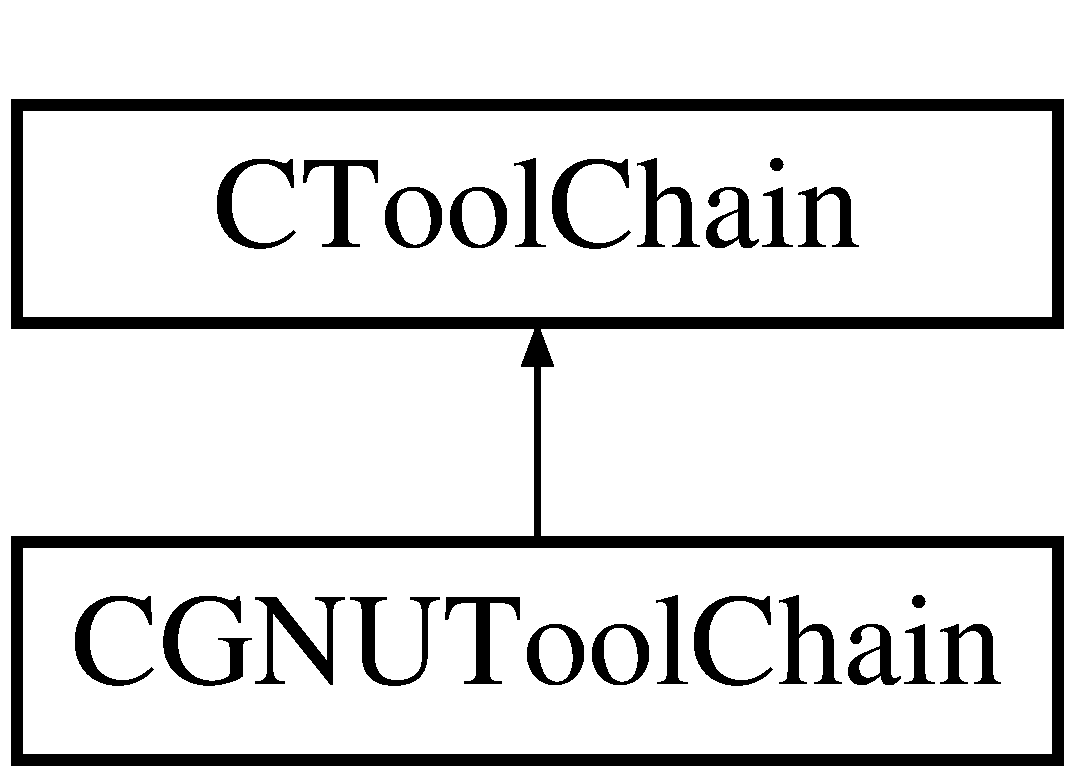
\includegraphics[height=2.000000cm]{d7/d26/classCGNUToolChain}
\end{center}
\end{figure}
\subsection*{Public Member Functions}
\begin{DoxyCompactItemize}
\item 
virtual \hyperlink{classCToolChain}{C\-Tool\-Chain} $\ast$ \hyperlink{classCGNUToolChain_a54793a226b09c673cce92a210d7fa471}{Create\-Instance} (void) const 
\item 
virtual void \hyperlink{classCGNUToolChain_ab989eae8567194074277acefff8eee2c}{Reset} (const \hyperlink{classCPlatform_a2fb735c63c53052f79629e338bb0f535}{C\-Platform\-::\-O\-S\-\_\-\-Type} \hyperlink{classCToolChain_abe4054d9081351e099163e2c53b260f8}{O\-S})
\item 
\hyperlink{classCGNUToolChain_aa5da10126f9b5a819ddc94d57e9947a4}{C\-G\-N\-U\-Tool\-Chain} (void)
\item 
virtual \hyperlink{classCGNUToolChain_a9f4fc82ffd121a68e43c95e5693295a8}{$\sim$\-C\-G\-N\-U\-Tool\-Chain} (void)
\end{DoxyCompactItemize}
\subsection*{Additional Inherited Members}


\subsection{Constructor \& Destructor Documentation}
\hypertarget{classCGNUToolChain_aa5da10126f9b5a819ddc94d57e9947a4}{\index{C\-G\-N\-U\-Tool\-Chain@{C\-G\-N\-U\-Tool\-Chain}!C\-G\-N\-U\-Tool\-Chain@{C\-G\-N\-U\-Tool\-Chain}}
\index{C\-G\-N\-U\-Tool\-Chain@{C\-G\-N\-U\-Tool\-Chain}!CGNUToolChain@{C\-G\-N\-U\-Tool\-Chain}}
\subsubsection[{C\-G\-N\-U\-Tool\-Chain}]{\setlength{\rightskip}{0pt plus 5cm}C\-G\-N\-U\-Tool\-Chain\-::\-C\-G\-N\-U\-Tool\-Chain (
\begin{DoxyParamCaption}
\item[{void}]{}
\end{DoxyParamCaption}
)}}\label{classCGNUToolChain_aa5da10126f9b5a819ddc94d57e9947a4}
\hypertarget{classCGNUToolChain_a9f4fc82ffd121a68e43c95e5693295a8}{\index{C\-G\-N\-U\-Tool\-Chain@{C\-G\-N\-U\-Tool\-Chain}!$\sim$\-C\-G\-N\-U\-Tool\-Chain@{$\sim$\-C\-G\-N\-U\-Tool\-Chain}}
\index{$\sim$\-C\-G\-N\-U\-Tool\-Chain@{$\sim$\-C\-G\-N\-U\-Tool\-Chain}!CGNUToolChain@{C\-G\-N\-U\-Tool\-Chain}}
\subsubsection[{$\sim$\-C\-G\-N\-U\-Tool\-Chain}]{\setlength{\rightskip}{0pt plus 5cm}C\-G\-N\-U\-Tool\-Chain\-::$\sim$\-C\-G\-N\-U\-Tool\-Chain (
\begin{DoxyParamCaption}
\item[{void}]{}
\end{DoxyParamCaption}
)\hspace{0.3cm}{\ttfamily [virtual]}}}\label{classCGNUToolChain_a9f4fc82ffd121a68e43c95e5693295a8}


\subsection{Member Function Documentation}
\hypertarget{classCGNUToolChain_a54793a226b09c673cce92a210d7fa471}{\index{C\-G\-N\-U\-Tool\-Chain@{C\-G\-N\-U\-Tool\-Chain}!Create\-Instance@{Create\-Instance}}
\index{Create\-Instance@{Create\-Instance}!CGNUToolChain@{C\-G\-N\-U\-Tool\-Chain}}
\subsubsection[{Create\-Instance}]{\setlength{\rightskip}{0pt plus 5cm}{\bf C\-Tool\-Chain} $\ast$ C\-G\-N\-U\-Tool\-Chain\-::\-Create\-Instance (
\begin{DoxyParamCaption}
\item[{void}]{}
\end{DoxyParamCaption}
) const\hspace{0.3cm}{\ttfamily [virtual]}}}\label{classCGNUToolChain_a54793a226b09c673cce92a210d7fa471}


Reimplemented from \hyperlink{classCToolChain_aa6765d5197d898efb01d032ac73b7764}{C\-Tool\-Chain}.

\hypertarget{classCGNUToolChain_ab989eae8567194074277acefff8eee2c}{\index{C\-G\-N\-U\-Tool\-Chain@{C\-G\-N\-U\-Tool\-Chain}!Reset@{Reset}}
\index{Reset@{Reset}!CGNUToolChain@{C\-G\-N\-U\-Tool\-Chain}}
\subsubsection[{Reset}]{\setlength{\rightskip}{0pt plus 5cm}void C\-G\-N\-U\-Tool\-Chain\-::\-Reset (
\begin{DoxyParamCaption}
\item[{const {\bf C\-Platform\-::\-O\-S\-\_\-\-Type}}]{O\-S}
\end{DoxyParamCaption}
)\hspace{0.3cm}{\ttfamily [virtual]}}}\label{classCGNUToolChain_ab989eae8567194074277acefff8eee2c}


Reimplemented from \hyperlink{classCToolChain_a3b48ddb23b898b3b6eaa356a2ed6fbf8}{C\-Tool\-Chain}.



The documentation for this class was generated from the following files\-:\begin{DoxyCompactItemize}
\item 
src/\hyperlink{toolchains_8h}{toolchains.\-h}\item 
src/\hyperlink{toolchains_8cpp}{toolchains.\-cpp}\end{DoxyCompactItemize}

\hypertarget{classCGNUWindowsResourceCompiler}{\section{C\-G\-N\-U\-Windows\-Resource\-Compiler Class Reference}
\label{classCGNUWindowsResourceCompiler}\index{C\-G\-N\-U\-Windows\-Resource\-Compiler@{C\-G\-N\-U\-Windows\-Resource\-Compiler}}
}


{\ttfamily \#include $<$buildtools.\-h$>$}

Inheritance diagram for C\-G\-N\-U\-Windows\-Resource\-Compiler\-:\begin{figure}[H]
\begin{center}
\leavevmode
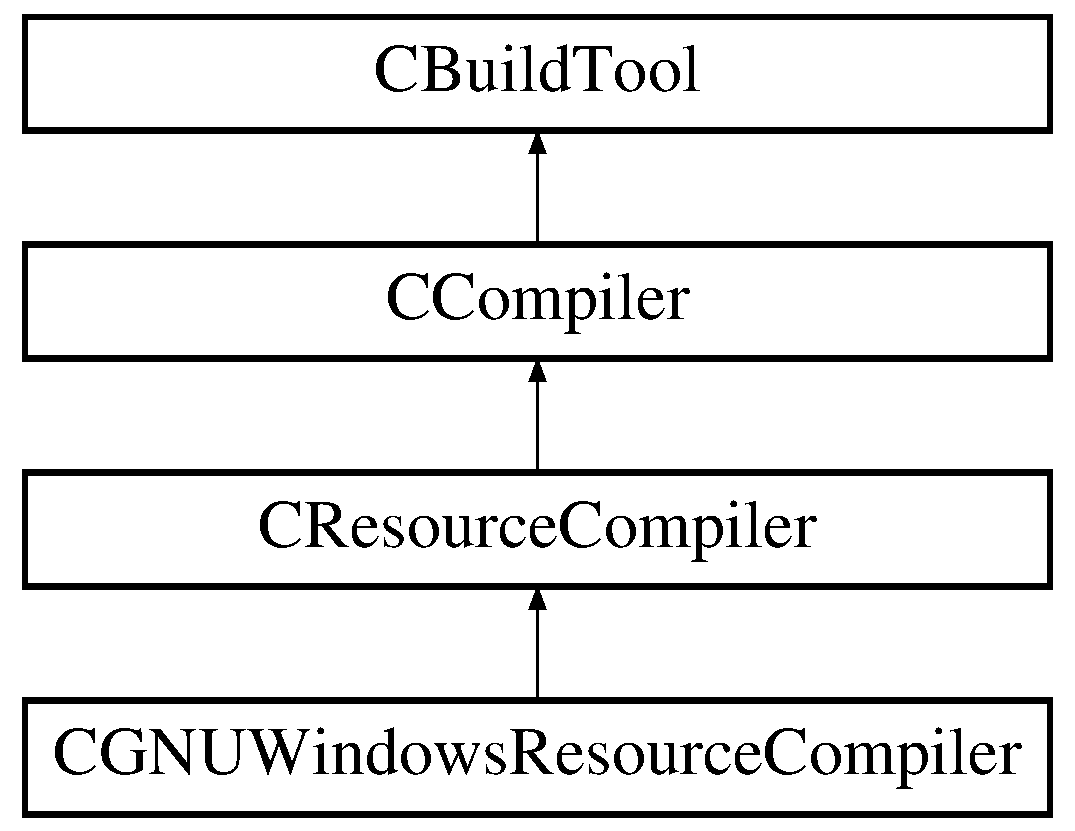
\includegraphics[height=4.000000cm]{d6/d3a/classCGNUWindowsResourceCompiler}
\end{center}
\end{figure}
\subsection*{Public Member Functions}
\begin{DoxyCompactItemize}
\item 
virtual \\*
\hyperlink{classCGNUWindowsResourceCompiler}{C\-G\-N\-U\-Windows\-Resource\-Compiler} $\ast$ \hyperlink{classCGNUWindowsResourceCompiler_a295b322f12aa797537c0ef38bed0a9a5}{Create\-Instance} (void)
\item 
virtual void \hyperlink{classCGNUWindowsResourceCompiler_add9c139a642cf1d18a3fb2978bb792c4}{Reset} (const \hyperlink{classCPlatform_a2fb735c63c53052f79629e338bb0f535}{C\-Platform\-::\-O\-S\-\_\-\-Type} O\-S)
\item 
virtual bool \hyperlink{classCGNUWindowsResourceCompiler_ac234523a2d9575abe309aa1814cf957d}{Supports} (const \hyperlink{classCPlatform_a2fb735c63c53052f79629e338bb0f535}{C\-Platform\-::\-O\-S\-\_\-\-Type} O\-S)
\item 
\hyperlink{classCGNUWindowsResourceCompiler_a70b137be8c68b0c1394b03901e4d1635}{C\-G\-N\-U\-Windows\-Resource\-Compiler} (void)
\end{DoxyCompactItemize}
\subsection*{Additional Inherited Members}


\subsection{Constructor \& Destructor Documentation}
\hypertarget{classCGNUWindowsResourceCompiler_a70b137be8c68b0c1394b03901e4d1635}{\index{C\-G\-N\-U\-Windows\-Resource\-Compiler@{C\-G\-N\-U\-Windows\-Resource\-Compiler}!C\-G\-N\-U\-Windows\-Resource\-Compiler@{C\-G\-N\-U\-Windows\-Resource\-Compiler}}
\index{C\-G\-N\-U\-Windows\-Resource\-Compiler@{C\-G\-N\-U\-Windows\-Resource\-Compiler}!CGNUWindowsResourceCompiler@{C\-G\-N\-U\-Windows\-Resource\-Compiler}}
\subsubsection[{C\-G\-N\-U\-Windows\-Resource\-Compiler}]{\setlength{\rightskip}{0pt plus 5cm}C\-G\-N\-U\-Windows\-Resource\-Compiler\-::\-C\-G\-N\-U\-Windows\-Resource\-Compiler (
\begin{DoxyParamCaption}
\item[{void}]{}
\end{DoxyParamCaption}
)}}\label{classCGNUWindowsResourceCompiler_a70b137be8c68b0c1394b03901e4d1635}


\subsection{Member Function Documentation}
\hypertarget{classCGNUWindowsResourceCompiler_a295b322f12aa797537c0ef38bed0a9a5}{\index{C\-G\-N\-U\-Windows\-Resource\-Compiler@{C\-G\-N\-U\-Windows\-Resource\-Compiler}!Create\-Instance@{Create\-Instance}}
\index{Create\-Instance@{Create\-Instance}!CGNUWindowsResourceCompiler@{C\-G\-N\-U\-Windows\-Resource\-Compiler}}
\subsubsection[{Create\-Instance}]{\setlength{\rightskip}{0pt plus 5cm}{\bf C\-G\-N\-U\-Windows\-Resource\-Compiler} $\ast$ C\-G\-N\-U\-Windows\-Resource\-Compiler\-::\-Create\-Instance (
\begin{DoxyParamCaption}
\item[{void}]{}
\end{DoxyParamCaption}
)\hspace{0.3cm}{\ttfamily [virtual]}}}\label{classCGNUWindowsResourceCompiler_a295b322f12aa797537c0ef38bed0a9a5}


Reimplemented from \hyperlink{classCResourceCompiler_a4f46ae1558a0096b040eb593d28a810c}{C\-Resource\-Compiler}.

\hypertarget{classCGNUWindowsResourceCompiler_add9c139a642cf1d18a3fb2978bb792c4}{\index{C\-G\-N\-U\-Windows\-Resource\-Compiler@{C\-G\-N\-U\-Windows\-Resource\-Compiler}!Reset@{Reset}}
\index{Reset@{Reset}!CGNUWindowsResourceCompiler@{C\-G\-N\-U\-Windows\-Resource\-Compiler}}
\subsubsection[{Reset}]{\setlength{\rightskip}{0pt plus 5cm}void C\-G\-N\-U\-Windows\-Resource\-Compiler\-::\-Reset (
\begin{DoxyParamCaption}
\item[{const {\bf C\-Platform\-::\-O\-S\-\_\-\-Type}}]{O\-S}
\end{DoxyParamCaption}
)\hspace{0.3cm}{\ttfamily [virtual]}}}\label{classCGNUWindowsResourceCompiler_add9c139a642cf1d18a3fb2978bb792c4}


Reimplemented from \hyperlink{classCBuildTool_abea21a0e61ab2177effdff5aaa169585}{C\-Build\-Tool}.

\hypertarget{classCGNUWindowsResourceCompiler_ac234523a2d9575abe309aa1814cf957d}{\index{C\-G\-N\-U\-Windows\-Resource\-Compiler@{C\-G\-N\-U\-Windows\-Resource\-Compiler}!Supports@{Supports}}
\index{Supports@{Supports}!CGNUWindowsResourceCompiler@{C\-G\-N\-U\-Windows\-Resource\-Compiler}}
\subsubsection[{Supports}]{\setlength{\rightskip}{0pt plus 5cm}bool C\-G\-N\-U\-Windows\-Resource\-Compiler\-::\-Supports (
\begin{DoxyParamCaption}
\item[{const {\bf C\-Platform\-::\-O\-S\-\_\-\-Type}}]{O\-S}
\end{DoxyParamCaption}
)\hspace{0.3cm}{\ttfamily [virtual]}}}\label{classCGNUWindowsResourceCompiler_ac234523a2d9575abe309aa1814cf957d}


Reimplemented from \hyperlink{classCBuildTool_ad07fcd46ccc841bc131d65505e5343c1}{C\-Build\-Tool}.



The documentation for this class was generated from the following files\-:\begin{DoxyCompactItemize}
\item 
src/\hyperlink{buildtools_8h}{buildtools.\-h}\item 
src/\hyperlink{buildtools_8cpp}{buildtools.\-cpp}\end{DoxyCompactItemize}

\hypertarget{classCIncludeSearchFilter}{\section{C\-Include\-Search\-Filter Class Reference}
\label{classCIncludeSearchFilter}\index{C\-Include\-Search\-Filter@{C\-Include\-Search\-Filter}}
}


Declares interface for gathering build unit dependencies from project files into build unit dependency database.  




{\ttfamily \#include $<$depsearch.\-h$>$}

Inheritance diagram for C\-Include\-Search\-Filter\-:\begin{figure}[H]
\begin{center}
\leavevmode
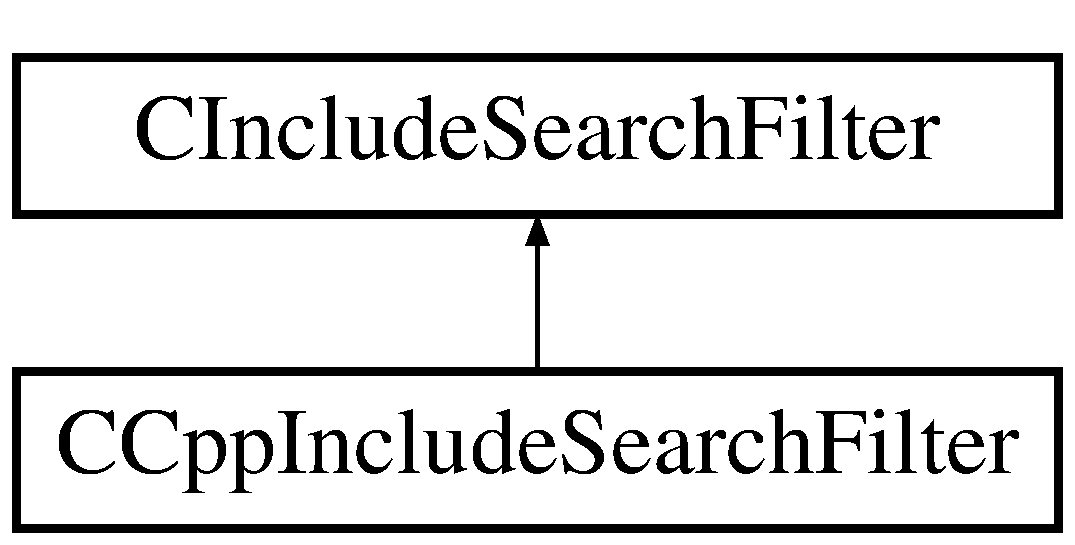
\includegraphics[height=2.000000cm]{d2/d24/classCIncludeSearchFilter}
\end{center}
\end{figure}
\subsection*{Public Member Functions}
\begin{DoxyCompactItemize}
\item 
virtual void \hyperlink{classCIncludeSearchFilter_a5effffa7de380a06feab27bdfde177a5}{Clear} (void)
\begin{DoxyCompactList}\small\item\em Resets the filter to the initial state. \end{DoxyCompactList}\item 
virtual void \hyperlink{classCIncludeSearchFilter_aa40e9e57c931219ab680beff78babb40}{Show} (void)
\begin{DoxyCompactList}\small\item\em Prints filter settings to standard output. \end{DoxyCompactList}\item 
virtual void \hyperlink{classCIncludeSearchFilter_adf262663be6dd431f048c61817ecb07a}{Assign} (const \hyperlink{classCIncludeSearchFilter}{C\-Include\-Search\-Filter} \&Filter)
\begin{DoxyCompactList}\small\item\em Copies filter settings from another filter. \end{DoxyCompactList}\item 
virtual bool \hyperlink{classCIncludeSearchFilter_a2b30667171e75cd5721e97b54eeb9182}{Execute} (const \hyperlink{classCString}{C\-String} \&File\-Name, \hyperlink{classCStringList}{C\-String\-List} \&Includes)
\begin{DoxyCompactList}\small\item\em Gathers dependencies to {\itshape Includes} string list starting from {\itshape File\-Name} file. \end{DoxyCompactList}\item 
virtual bool \hyperlink{classCIncludeSearchFilter_aa43b2d4b8f62c9d695490d5cd072c3bc}{Execute} (const \hyperlink{classCString}{C\-String} \&File\-Name, \hyperlink{classCDependencyInfo}{C\-Dependency\-Info} \&Dependencies)
\begin{DoxyCompactList}\small\item\em Gathers dependencies to {\itshape Dependencies} database starting from {\itshape File\-Name} file. \end{DoxyCompactList}\item 
void \hyperlink{classCIncludeSearchFilter_a5716c9dc6d07feaeeaab44a7fe65bdcb}{Add\-Include\-Directory} (const \hyperlink{classCString}{C\-String} \&Path)
\begin{DoxyCompactList}\small\item\em Adds {\itshape Path} path to the list of unit lookup directories. \end{DoxyCompactList}\item 
void \hyperlink{classCIncludeSearchFilter_a7d91b0a6d6bb3b0dacca02a47f0bc1d2}{Add\-Include\-Directories} (const \hyperlink{classCStringList}{C\-String\-List} \&Paths)
\begin{DoxyCompactList}\small\item\em Adds {\itshape Paths} list of paths to the list of unit lookup directories. \end{DoxyCompactList}\item 
void \hyperlink{classCIncludeSearchFilter_a1f9de2b494d146bc2df210c7524c153b}{Add\-Macro\-Definiton} (const \hyperlink{classCString}{C\-String} \&Macro)
\begin{DoxyCompactList}\small\item\em Adds {\itshape Macro} macro to the list of macros. \end{DoxyCompactList}\item 
void \hyperlink{classCIncludeSearchFilter_ab5bd5e9e177f90b6bbe29d4a4ea83f41}{Add\-Macro\-Definitons} (const \hyperlink{classCStringList}{C\-String\-List} \&Macros)
\begin{DoxyCompactList}\small\item\em Adds {\itshape Macros} macros to the list of macros. \end{DoxyCompactList}\item 
\hyperlink{classCString}{C\-String} \hyperlink{classCIncludeSearchFilter_a89c3d026fb68931212d397dff94ede64}{Resolve\-Include\-Path} (const \hyperlink{classCString}{C\-String} \&Include\-Name)
\begin{DoxyCompactList}\small\item\em Resolves a build unit file name into complete file path. \end{DoxyCompactList}\item 
\hyperlink{classCIncludeSearchFilter_ab3fbb998a1ff29e3c33e5bb296780bec}{C\-Include\-Search\-Filter} (void)
\begin{DoxyCompactList}\small\item\em Creates dependency search filter. \end{DoxyCompactList}\item 
\hyperlink{classCIncludeSearchFilter_ae38d64230ed0a36bce60b0e4a3a9759e}{C\-Include\-Search\-Filter} (const \hyperlink{classCIncludeSearchFilter}{C\-Include\-Search\-Filter} \&Filter)
\begin{DoxyCompactList}\small\item\em Copies dependency search filter from another filter. \end{DoxyCompactList}\item 
\hyperlink{classCIncludeSearchFilter_a54b44f1662a196e45d49d2155ba3eef2}{$\sim$\-C\-Include\-Search\-Filter} (void)
\begin{DoxyCompactList}\small\item\em Destroys dependency search filter. \end{DoxyCompactList}\end{DoxyCompactItemize}
\subsection*{Protected Attributes}
\begin{DoxyCompactItemize}
\item 
\hyperlink{classCStringList}{C\-String\-List} \hyperlink{classCIncludeSearchFilter_a888266f23bb4769ba0c931e285c04015}{m\-\_\-\-Include\-Directories}
\begin{DoxyCompactList}\small\item\em a list of directories to look for build units. \end{DoxyCompactList}\item 
\hyperlink{classCStringList}{C\-String\-List} \hyperlink{classCIncludeSearchFilter_af5c1083b429ed970c5ae8bce126e726d}{m\-\_\-\-Defined\-Macros}
\begin{DoxyCompactList}\small\item\em a list of preprocessor's macro defnitions. \end{DoxyCompactList}\end{DoxyCompactItemize}


\subsection{Detailed Description}
Declares interface for gathering build unit dependencies from project files into build unit dependency database. 

\subsection{Constructor \& Destructor Documentation}
\hypertarget{classCIncludeSearchFilter_ab3fbb998a1ff29e3c33e5bb296780bec}{\index{C\-Include\-Search\-Filter@{C\-Include\-Search\-Filter}!C\-Include\-Search\-Filter@{C\-Include\-Search\-Filter}}
\index{C\-Include\-Search\-Filter@{C\-Include\-Search\-Filter}!CIncludeSearchFilter@{C\-Include\-Search\-Filter}}
\subsubsection[{C\-Include\-Search\-Filter}]{\setlength{\rightskip}{0pt plus 5cm}C\-Include\-Search\-Filter\-::\-C\-Include\-Search\-Filter (
\begin{DoxyParamCaption}
\item[{void}]{}
\end{DoxyParamCaption}
)}}\label{classCIncludeSearchFilter_ab3fbb998a1ff29e3c33e5bb296780bec}


Creates dependency search filter. 

\hypertarget{classCIncludeSearchFilter_ae38d64230ed0a36bce60b0e4a3a9759e}{\index{C\-Include\-Search\-Filter@{C\-Include\-Search\-Filter}!C\-Include\-Search\-Filter@{C\-Include\-Search\-Filter}}
\index{C\-Include\-Search\-Filter@{C\-Include\-Search\-Filter}!CIncludeSearchFilter@{C\-Include\-Search\-Filter}}
\subsubsection[{C\-Include\-Search\-Filter}]{\setlength{\rightskip}{0pt plus 5cm}C\-Include\-Search\-Filter\-::\-C\-Include\-Search\-Filter (
\begin{DoxyParamCaption}
\item[{const {\bf C\-Include\-Search\-Filter} \&}]{Filter}
\end{DoxyParamCaption}
)}}\label{classCIncludeSearchFilter_ae38d64230ed0a36bce60b0e4a3a9759e}


Copies dependency search filter from another filter. 


\begin{DoxyParams}{Parameters}
{\em Filter} & another dependency search filter. \\
\hline
\end{DoxyParams}
\hypertarget{classCIncludeSearchFilter_a54b44f1662a196e45d49d2155ba3eef2}{\index{C\-Include\-Search\-Filter@{C\-Include\-Search\-Filter}!$\sim$\-C\-Include\-Search\-Filter@{$\sim$\-C\-Include\-Search\-Filter}}
\index{$\sim$\-C\-Include\-Search\-Filter@{$\sim$\-C\-Include\-Search\-Filter}!CIncludeSearchFilter@{C\-Include\-Search\-Filter}}
\subsubsection[{$\sim$\-C\-Include\-Search\-Filter}]{\setlength{\rightskip}{0pt plus 5cm}C\-Include\-Search\-Filter\-::$\sim$\-C\-Include\-Search\-Filter (
\begin{DoxyParamCaption}
\item[{void}]{}
\end{DoxyParamCaption}
)}}\label{classCIncludeSearchFilter_a54b44f1662a196e45d49d2155ba3eef2}


Destroys dependency search filter. 



\subsection{Member Function Documentation}
\hypertarget{classCIncludeSearchFilter_a7d91b0a6d6bb3b0dacca02a47f0bc1d2}{\index{C\-Include\-Search\-Filter@{C\-Include\-Search\-Filter}!Add\-Include\-Directories@{Add\-Include\-Directories}}
\index{Add\-Include\-Directories@{Add\-Include\-Directories}!CIncludeSearchFilter@{C\-Include\-Search\-Filter}}
\subsubsection[{Add\-Include\-Directories}]{\setlength{\rightskip}{0pt plus 5cm}C\-Include\-Search\-Filter\-::\-Add\-Include\-Directories (
\begin{DoxyParamCaption}
\item[{const {\bf C\-String\-List} \&}]{Paths}
\end{DoxyParamCaption}
)}}\label{classCIncludeSearchFilter_a7d91b0a6d6bb3b0dacca02a47f0bc1d2}


Adds {\itshape Paths} list of paths to the list of unit lookup directories. 


\begin{DoxyParams}{Parameters}
{\em Paths} & a list of directories. \\
\hline
\end{DoxyParams}
\hypertarget{classCIncludeSearchFilter_a5716c9dc6d07feaeeaab44a7fe65bdcb}{\index{C\-Include\-Search\-Filter@{C\-Include\-Search\-Filter}!Add\-Include\-Directory@{Add\-Include\-Directory}}
\index{Add\-Include\-Directory@{Add\-Include\-Directory}!CIncludeSearchFilter@{C\-Include\-Search\-Filter}}
\subsubsection[{Add\-Include\-Directory}]{\setlength{\rightskip}{0pt plus 5cm}C\-Include\-Search\-Filter\-::\-Add\-Include\-Directory (
\begin{DoxyParamCaption}
\item[{const {\bf C\-String} \&}]{Path}
\end{DoxyParamCaption}
)}}\label{classCIncludeSearchFilter_a5716c9dc6d07feaeeaab44a7fe65bdcb}


Adds {\itshape Path} path to the list of unit lookup directories. 


\begin{DoxyParams}{Parameters}
{\em Path} & a directory path. \\
\hline
\end{DoxyParams}
\hypertarget{classCIncludeSearchFilter_a1f9de2b494d146bc2df210c7524c153b}{\index{C\-Include\-Search\-Filter@{C\-Include\-Search\-Filter}!Add\-Macro\-Definiton@{Add\-Macro\-Definiton}}
\index{Add\-Macro\-Definiton@{Add\-Macro\-Definiton}!CIncludeSearchFilter@{C\-Include\-Search\-Filter}}
\subsubsection[{Add\-Macro\-Definiton}]{\setlength{\rightskip}{0pt plus 5cm}C\-Include\-Search\-Filter\-::\-Add\-Macro\-Definiton (
\begin{DoxyParamCaption}
\item[{const {\bf C\-String} \&}]{Macro}
\end{DoxyParamCaption}
)}}\label{classCIncludeSearchFilter_a1f9de2b494d146bc2df210c7524c153b}


Adds {\itshape Macro} macro to the list of macros. 


\begin{DoxyParams}{Parameters}
{\em Macro} & name of a macro definition. \\
\hline
\end{DoxyParams}
\hypertarget{classCIncludeSearchFilter_ab5bd5e9e177f90b6bbe29d4a4ea83f41}{\index{C\-Include\-Search\-Filter@{C\-Include\-Search\-Filter}!Add\-Macro\-Definitons@{Add\-Macro\-Definitons}}
\index{Add\-Macro\-Definitons@{Add\-Macro\-Definitons}!CIncludeSearchFilter@{C\-Include\-Search\-Filter}}
\subsubsection[{Add\-Macro\-Definitons}]{\setlength{\rightskip}{0pt plus 5cm}C\-Include\-Search\-Filter\-::\-Add\-Macro\-Definitons (
\begin{DoxyParamCaption}
\item[{const {\bf C\-String\-List} \&}]{Macros}
\end{DoxyParamCaption}
)}}\label{classCIncludeSearchFilter_ab5bd5e9e177f90b6bbe29d4a4ea83f41}


Adds {\itshape Macros} macros to the list of macros. 


\begin{DoxyParams}{Parameters}
{\em Macros} & a list of names of macro definitions. \\
\hline
\end{DoxyParams}
\hypertarget{classCIncludeSearchFilter_adf262663be6dd431f048c61817ecb07a}{\index{C\-Include\-Search\-Filter@{C\-Include\-Search\-Filter}!Assign@{Assign}}
\index{Assign@{Assign}!CIncludeSearchFilter@{C\-Include\-Search\-Filter}}
\subsubsection[{Assign}]{\setlength{\rightskip}{0pt plus 5cm}C\-Include\-Search\-Filter\-::\-Assign (
\begin{DoxyParamCaption}
\item[{const {\bf C\-Include\-Search\-Filter} \&}]{Filter}
\end{DoxyParamCaption}
)\hspace{0.3cm}{\ttfamily [virtual]}}}\label{classCIncludeSearchFilter_adf262663be6dd431f048c61817ecb07a}


Copies filter settings from another filter. 


\begin{DoxyParams}{Parameters}
{\em Filter} & another filter. \\
\hline
\end{DoxyParams}
\hypertarget{classCIncludeSearchFilter_a5effffa7de380a06feab27bdfde177a5}{\index{C\-Include\-Search\-Filter@{C\-Include\-Search\-Filter}!Clear@{Clear}}
\index{Clear@{Clear}!CIncludeSearchFilter@{C\-Include\-Search\-Filter}}
\subsubsection[{Clear}]{\setlength{\rightskip}{0pt plus 5cm}C\-Include\-Search\-Filter\-::\-Clear (
\begin{DoxyParamCaption}
\item[{void}]{}
\end{DoxyParamCaption}
)\hspace{0.3cm}{\ttfamily [virtual]}}}\label{classCIncludeSearchFilter_a5effffa7de380a06feab27bdfde177a5}


Resets the filter to the initial state. 

\hypertarget{classCIncludeSearchFilter_a2b30667171e75cd5721e97b54eeb9182}{\index{C\-Include\-Search\-Filter@{C\-Include\-Search\-Filter}!Execute@{Execute}}
\index{Execute@{Execute}!CIncludeSearchFilter@{C\-Include\-Search\-Filter}}
\subsubsection[{Execute}]{\setlength{\rightskip}{0pt plus 5cm}C\-Include\-Search\-Filter\-::\-Execute (
\begin{DoxyParamCaption}
\item[{const {\bf C\-String} \&}]{File\-Name, }
\item[{{\bf C\-String\-List} \&}]{Includes}
\end{DoxyParamCaption}
)\hspace{0.3cm}{\ttfamily [virtual]}}}\label{classCIncludeSearchFilter_a2b30667171e75cd5721e97b54eeb9182}


Gathers dependencies to {\itshape Includes} string list starting from {\itshape File\-Name} file. 

\begin{DoxyRefDesc}{Deprecated}
\item[\hyperlink{deprecated__deprecated000001}{Deprecated}]Use \hyperlink{classCIncludeSearchFilter_aa43b2d4b8f62c9d695490d5cd072c3bc}{C\-Include\-Search\-Filter\-::\-Execute(const C\-String\& File\-Name, C\-Dependency\-Info\& Dependencies)}.\end{DoxyRefDesc}

\begin{DoxyParams}{Parameters}
{\em File\-Name} & a build unit name. \\
\hline
{\em Includes} & a list of build unit names. \\
\hline
\end{DoxyParams}
\begin{DoxyReturn}{Returns}
{\itshape true} if dependencies were gather from at least one (starting) file, {\itshape false} otherwise. 
\end{DoxyReturn}


Reimplemented in \hyperlink{classCCppIncludeSearchFilter_a847f213a3ab4d7220a1ee0a095a5f42f}{C\-Cpp\-Include\-Search\-Filter}.

\hypertarget{classCIncludeSearchFilter_aa43b2d4b8f62c9d695490d5cd072c3bc}{\index{C\-Include\-Search\-Filter@{C\-Include\-Search\-Filter}!Execute@{Execute}}
\index{Execute@{Execute}!CIncludeSearchFilter@{C\-Include\-Search\-Filter}}
\subsubsection[{Execute}]{\setlength{\rightskip}{0pt plus 5cm}C\-Include\-Search\-Filter\-::\-Execute (
\begin{DoxyParamCaption}
\item[{const {\bf C\-String} \&}]{File\-Name, }
\item[{{\bf C\-Dependency\-Info} \&}]{Dependencies}
\end{DoxyParamCaption}
)\hspace{0.3cm}{\ttfamily [virtual]}}}\label{classCIncludeSearchFilter_aa43b2d4b8f62c9d695490d5cd072c3bc}


Gathers dependencies to {\itshape Dependencies} database starting from {\itshape File\-Name} file. 


\begin{DoxyParams}{Parameters}
{\em File\-Name} & a build unit name. \\
\hline
{\em Dependencies} & a build unit dependency database. \\
\hline
\end{DoxyParams}
\begin{DoxyReturn}{Returns}
{\itshape true} if dependencies were gather from at least one (starting) file, {\itshape false} otherwise. 
\end{DoxyReturn}


Reimplemented in \hyperlink{classCCppIncludeSearchFilter_ac37bc3584c554db6a7964c8e9de31636}{C\-Cpp\-Include\-Search\-Filter}.

\hypertarget{classCIncludeSearchFilter_a89c3d026fb68931212d397dff94ede64}{\index{C\-Include\-Search\-Filter@{C\-Include\-Search\-Filter}!Resolve\-Include\-Path@{Resolve\-Include\-Path}}
\index{Resolve\-Include\-Path@{Resolve\-Include\-Path}!CIncludeSearchFilter@{C\-Include\-Search\-Filter}}
\subsubsection[{Resolve\-Include\-Path}]{\setlength{\rightskip}{0pt plus 5cm}C\-Include\-Search\-Filter\-::\-Resolve\-Include\-Path (
\begin{DoxyParamCaption}
\item[{const {\bf C\-String} \&}]{Include\-Name}
\end{DoxyParamCaption}
)}}\label{classCIncludeSearchFilter_a89c3d026fb68931212d397dff94ede64}


Resolves a build unit file name into complete file path. 


\begin{DoxyParams}{Parameters}
{\em Include\-Name} & a build unit file name. \\
\hline
\end{DoxyParams}
\begin{DoxyReturn}{Returns}
file path to the build unit if it is successfully found or an empty string if it can't be found. 
\end{DoxyReturn}
\hypertarget{classCIncludeSearchFilter_aa40e9e57c931219ab680beff78babb40}{\index{C\-Include\-Search\-Filter@{C\-Include\-Search\-Filter}!Show@{Show}}
\index{Show@{Show}!CIncludeSearchFilter@{C\-Include\-Search\-Filter}}
\subsubsection[{Show}]{\setlength{\rightskip}{0pt plus 5cm}C\-Include\-Search\-Filter\-::\-Show (
\begin{DoxyParamCaption}
\item[{void}]{}
\end{DoxyParamCaption}
)\hspace{0.3cm}{\ttfamily [virtual]}}}\label{classCIncludeSearchFilter_aa40e9e57c931219ab680beff78babb40}


Prints filter settings to standard output. 



\subsection{Member Data Documentation}
\hypertarget{classCIncludeSearchFilter_af5c1083b429ed970c5ae8bce126e726d}{\index{C\-Include\-Search\-Filter@{C\-Include\-Search\-Filter}!m\-\_\-\-Defined\-Macros@{m\-\_\-\-Defined\-Macros}}
\index{m\-\_\-\-Defined\-Macros@{m\-\_\-\-Defined\-Macros}!CIncludeSearchFilter@{C\-Include\-Search\-Filter}}
\subsubsection[{m\-\_\-\-Defined\-Macros}]{\setlength{\rightskip}{0pt plus 5cm}C\-Include\-Search\-Filter\-::m\-\_\-\-Defined\-Macros\hspace{0.3cm}{\ttfamily [protected]}}}\label{classCIncludeSearchFilter_af5c1083b429ed970c5ae8bce126e726d}


a list of preprocessor's macro defnitions. 

\hypertarget{classCIncludeSearchFilter_a888266f23bb4769ba0c931e285c04015}{\index{C\-Include\-Search\-Filter@{C\-Include\-Search\-Filter}!m\-\_\-\-Include\-Directories@{m\-\_\-\-Include\-Directories}}
\index{m\-\_\-\-Include\-Directories@{m\-\_\-\-Include\-Directories}!CIncludeSearchFilter@{C\-Include\-Search\-Filter}}
\subsubsection[{m\-\_\-\-Include\-Directories}]{\setlength{\rightskip}{0pt plus 5cm}C\-Include\-Search\-Filter\-::m\-\_\-\-Include\-Directories\hspace{0.3cm}{\ttfamily [protected]}}}\label{classCIncludeSearchFilter_a888266f23bb4769ba0c931e285c04015}


a list of directories to look for build units. 



The documentation for this class was generated from the following files\-:\begin{DoxyCompactItemize}
\item 
src/\hyperlink{depsearch_8h}{depsearch.\-h}\item 
src/\hyperlink{depsearch_8cpp}{depsearch.\-cpp}\item 
src/doc/\hyperlink{depsearch_8dox}{depsearch.\-dox}\end{DoxyCompactItemize}

\hypertarget{classCIntegerVariable}{\section{C\-Integer\-Variable Class Reference}
\label{classCIntegerVariable}\index{C\-Integer\-Variable@{C\-Integer\-Variable}}
}


{\ttfamily \#include $<$stlvariables.\-h$>$}

Inheritance diagram for C\-Integer\-Variable\-:\begin{figure}[H]
\begin{center}
\leavevmode
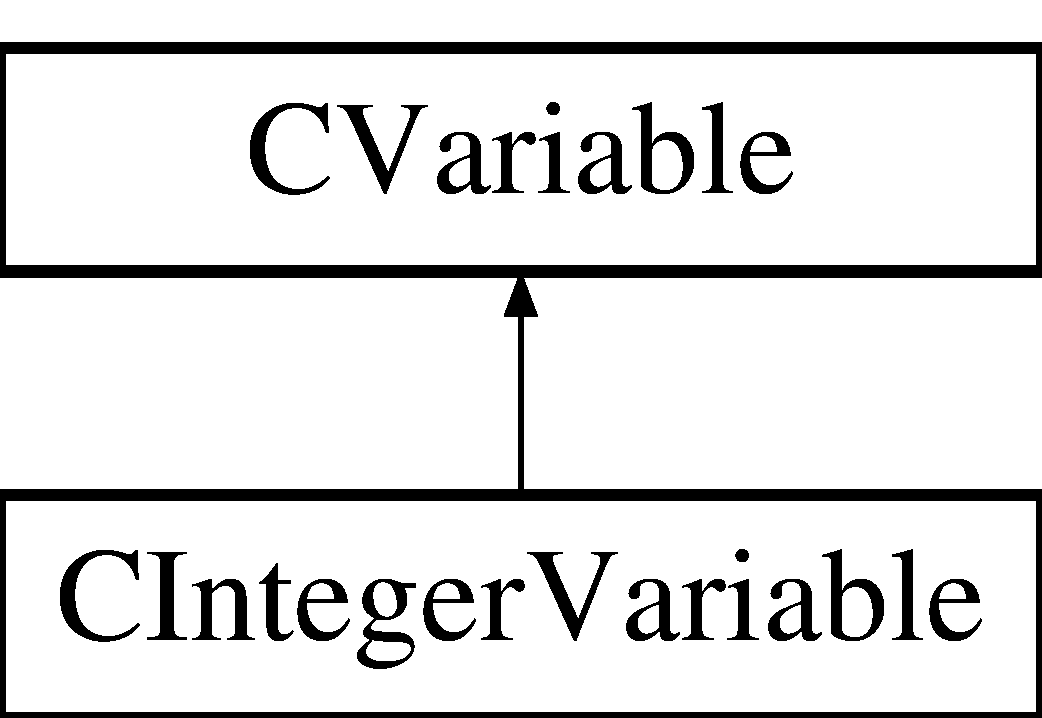
\includegraphics[height=2.000000cm]{de/db5/classCIntegerVariable}
\end{center}
\end{figure}
\subsection*{Public Member Functions}
\begin{DoxyCompactItemize}
\item 
virtual int \hyperlink{classCIntegerVariable_aed1d50a3a0570877bbfd1c942214209b}{Get\-Type} (void) const 
\item 
virtual \hyperlink{classCString}{C\-String} \hyperlink{classCIntegerVariable_aab3fb2ea2f634ccfc965d7adfeabab8a}{Get\-Type\-Name} (void) const 
\item 
virtual double \hyperlink{classCIntegerVariable_a5b993f4518f52b3b0c109b7bc74389ee}{Get\-Float} (void) const 
\item 
virtual void \hyperlink{classCIntegerVariable_ac5a68b16aba5348cc4a563c2771eda02}{Set\-Float} (const double Value)
\item 
virtual int \hyperlink{classCIntegerVariable_a24cfccaf406f0bd652241e2e0f2e928a}{Get\-Integer} (void) const 
\item 
virtual void \hyperlink{classCIntegerVariable_a2e00b834d4019241da2a32b8a7ad4a64}{Set\-Integer} (const int Value)
\item 
virtual bool \hyperlink{classCIntegerVariable_a62362a25f9cab7a3aba600ca42666bfa}{Get\-Boolean} (void) const 
\item 
virtual void \hyperlink{classCIntegerVariable_aceb8db208cad92ea4c7846fe2c0992d0}{Set\-Boolean} (const bool Value)
\item 
virtual \hyperlink{classCString}{C\-String} \hyperlink{classCIntegerVariable_a44c1bda15c10f0161046adf9c81d54d4}{Get\-String} (void) const 
\item 
virtual void \hyperlink{classCIntegerVariable_aa66b305e3ced11d63c64e7400f4d0434}{Set\-String} (const \hyperlink{classCString}{C\-String} \&Value)
\item 
virtual char \hyperlink{classCIntegerVariable_a93944292c5605b75906dbb2f55c0ab38}{Get\-Char} (void) const 
\item 
virtual void \hyperlink{classCIntegerVariable_a02ad451cbd589022a0761d3e8c62280c}{Set\-Char} (const char Value)
\item 
int \hyperlink{classCIntegerVariable_a434336429ffa52bb8bc1b9281a380b91}{operator=} (const \hyperlink{classCIntegerVariable}{C\-Integer\-Variable} \&Variable)
\item 
\hyperlink{classCIntegerVariable}{C\-Integer\-Variable} \& \hyperlink{classCIntegerVariable_ad2b015e2ab95995c4d3ace9712e0e98d}{operator=} (const double Value)
\item 
\hyperlink{classCIntegerVariable}{C\-Integer\-Variable} \& \hyperlink{classCIntegerVariable_a24e2febceadf0004896f338e971f7b2f}{operator=} (const int Value)
\item 
\hyperlink{classCIntegerVariable}{C\-Integer\-Variable} \& \hyperlink{classCIntegerVariable_a26c0a8db598c0a103b47c7279140cb53}{operator=} (const bool Value)
\item 
\hyperlink{classCIntegerVariable}{C\-Integer\-Variable} \& \hyperlink{classCIntegerVariable_ac088b36bdcfb0d474f2ba089fa2966c5}{operator=} (const \hyperlink{classCString}{C\-String} \&Value)
\item 
\hyperlink{classCIntegerVariable}{C\-Integer\-Variable} \& \hyperlink{classCIntegerVariable_a17c76d8904b4dc3adf203b58d1fb6a49}{operator=} (const char Value)
\item 
\hyperlink{classCIntegerVariable_aba557b8b31de66456c4c8fa3e464377d}{C\-Integer\-Variable} (const \hyperlink{classCString}{C\-String} \&Name, const int Value=0)
\item 
virtual \hyperlink{classCIntegerVariable_ad323afce088ff8252828a0ed19c0a5ec}{$\sim$\-C\-Integer\-Variable} (void)
\end{DoxyCompactItemize}
\subsection*{Protected Attributes}
\begin{DoxyCompactItemize}
\item 
int \hyperlink{classCIntegerVariable_af7a7c03be481414a895c17b777bfc148}{m\-\_\-\-Value}
\end{DoxyCompactItemize}


\subsection{Constructor \& Destructor Documentation}
\hypertarget{classCIntegerVariable_aba557b8b31de66456c4c8fa3e464377d}{\index{C\-Integer\-Variable@{C\-Integer\-Variable}!C\-Integer\-Variable@{C\-Integer\-Variable}}
\index{C\-Integer\-Variable@{C\-Integer\-Variable}!CIntegerVariable@{C\-Integer\-Variable}}
\subsubsection[{C\-Integer\-Variable}]{\setlength{\rightskip}{0pt plus 5cm}C\-Integer\-Variable\-::\-C\-Integer\-Variable (
\begin{DoxyParamCaption}
\item[{const {\bf C\-String} \&}]{Name, }
\item[{const int}]{Value = {\ttfamily 0}}
\end{DoxyParamCaption}
)}}\label{classCIntegerVariable_aba557b8b31de66456c4c8fa3e464377d}
\hypertarget{classCIntegerVariable_ad323afce088ff8252828a0ed19c0a5ec}{\index{C\-Integer\-Variable@{C\-Integer\-Variable}!$\sim$\-C\-Integer\-Variable@{$\sim$\-C\-Integer\-Variable}}
\index{$\sim$\-C\-Integer\-Variable@{$\sim$\-C\-Integer\-Variable}!CIntegerVariable@{C\-Integer\-Variable}}
\subsubsection[{$\sim$\-C\-Integer\-Variable}]{\setlength{\rightskip}{0pt plus 5cm}virtual C\-Integer\-Variable\-::$\sim$\-C\-Integer\-Variable (
\begin{DoxyParamCaption}
\item[{void}]{}
\end{DoxyParamCaption}
)\hspace{0.3cm}{\ttfamily [inline]}, {\ttfamily [virtual]}}}\label{classCIntegerVariable_ad323afce088ff8252828a0ed19c0a5ec}


\subsection{Member Function Documentation}
\hypertarget{classCIntegerVariable_a62362a25f9cab7a3aba600ca42666bfa}{\index{C\-Integer\-Variable@{C\-Integer\-Variable}!Get\-Boolean@{Get\-Boolean}}
\index{Get\-Boolean@{Get\-Boolean}!CIntegerVariable@{C\-Integer\-Variable}}
\subsubsection[{Get\-Boolean}]{\setlength{\rightskip}{0pt plus 5cm}bool C\-Integer\-Variable\-::\-Get\-Boolean (
\begin{DoxyParamCaption}
\item[{void}]{}
\end{DoxyParamCaption}
) const\hspace{0.3cm}{\ttfamily [virtual]}}}\label{classCIntegerVariable_a62362a25f9cab7a3aba600ca42666bfa}


Reimplemented from \hyperlink{classCVariable_a874156d6b1a3a44f799c32a2455c7f49}{C\-Variable}.

\hypertarget{classCIntegerVariable_a93944292c5605b75906dbb2f55c0ab38}{\index{C\-Integer\-Variable@{C\-Integer\-Variable}!Get\-Char@{Get\-Char}}
\index{Get\-Char@{Get\-Char}!CIntegerVariable@{C\-Integer\-Variable}}
\subsubsection[{Get\-Char}]{\setlength{\rightskip}{0pt plus 5cm}char C\-Integer\-Variable\-::\-Get\-Char (
\begin{DoxyParamCaption}
\item[{void}]{}
\end{DoxyParamCaption}
) const\hspace{0.3cm}{\ttfamily [virtual]}}}\label{classCIntegerVariable_a93944292c5605b75906dbb2f55c0ab38}


Reimplemented from \hyperlink{classCVariable_a6635a8fd2441dcb83a39d10a78187dac}{C\-Variable}.

\hypertarget{classCIntegerVariable_a5b993f4518f52b3b0c109b7bc74389ee}{\index{C\-Integer\-Variable@{C\-Integer\-Variable}!Get\-Float@{Get\-Float}}
\index{Get\-Float@{Get\-Float}!CIntegerVariable@{C\-Integer\-Variable}}
\subsubsection[{Get\-Float}]{\setlength{\rightskip}{0pt plus 5cm}double C\-Integer\-Variable\-::\-Get\-Float (
\begin{DoxyParamCaption}
\item[{void}]{}
\end{DoxyParamCaption}
) const\hspace{0.3cm}{\ttfamily [virtual]}}}\label{classCIntegerVariable_a5b993f4518f52b3b0c109b7bc74389ee}


Reimplemented from \hyperlink{classCVariable_ac475ad87ffbfaeeb2d4d9c2986b0d575}{C\-Variable}.

\hypertarget{classCIntegerVariable_a24cfccaf406f0bd652241e2e0f2e928a}{\index{C\-Integer\-Variable@{C\-Integer\-Variable}!Get\-Integer@{Get\-Integer}}
\index{Get\-Integer@{Get\-Integer}!CIntegerVariable@{C\-Integer\-Variable}}
\subsubsection[{Get\-Integer}]{\setlength{\rightskip}{0pt plus 5cm}int C\-Integer\-Variable\-::\-Get\-Integer (
\begin{DoxyParamCaption}
\item[{void}]{}
\end{DoxyParamCaption}
) const\hspace{0.3cm}{\ttfamily [virtual]}}}\label{classCIntegerVariable_a24cfccaf406f0bd652241e2e0f2e928a}


Reimplemented from \hyperlink{classCVariable_adb0db49f4a55f3e1b5322f6ce26e4ebc}{C\-Variable}.

\hypertarget{classCIntegerVariable_a44c1bda15c10f0161046adf9c81d54d4}{\index{C\-Integer\-Variable@{C\-Integer\-Variable}!Get\-String@{Get\-String}}
\index{Get\-String@{Get\-String}!CIntegerVariable@{C\-Integer\-Variable}}
\subsubsection[{Get\-String}]{\setlength{\rightskip}{0pt plus 5cm}{\bf C\-String} C\-Integer\-Variable\-::\-Get\-String (
\begin{DoxyParamCaption}
\item[{void}]{}
\end{DoxyParamCaption}
) const\hspace{0.3cm}{\ttfamily [virtual]}}}\label{classCIntegerVariable_a44c1bda15c10f0161046adf9c81d54d4}


Reimplemented from \hyperlink{classCVariable_aefa25c880c0042ffc29889475d329004}{C\-Variable}.

\hypertarget{classCIntegerVariable_aed1d50a3a0570877bbfd1c942214209b}{\index{C\-Integer\-Variable@{C\-Integer\-Variable}!Get\-Type@{Get\-Type}}
\index{Get\-Type@{Get\-Type}!CIntegerVariable@{C\-Integer\-Variable}}
\subsubsection[{Get\-Type}]{\setlength{\rightskip}{0pt plus 5cm}int C\-Integer\-Variable\-::\-Get\-Type (
\begin{DoxyParamCaption}
\item[{void}]{}
\end{DoxyParamCaption}
) const\hspace{0.3cm}{\ttfamily [virtual]}}}\label{classCIntegerVariable_aed1d50a3a0570877bbfd1c942214209b}


Reimplemented from \hyperlink{classCVariable_acdf7301ad2f5c7fa33770c028211c0bc}{C\-Variable}.

\hypertarget{classCIntegerVariable_aab3fb2ea2f634ccfc965d7adfeabab8a}{\index{C\-Integer\-Variable@{C\-Integer\-Variable}!Get\-Type\-Name@{Get\-Type\-Name}}
\index{Get\-Type\-Name@{Get\-Type\-Name}!CIntegerVariable@{C\-Integer\-Variable}}
\subsubsection[{Get\-Type\-Name}]{\setlength{\rightskip}{0pt plus 5cm}{\bf C\-String} C\-Integer\-Variable\-::\-Get\-Type\-Name (
\begin{DoxyParamCaption}
\item[{void}]{}
\end{DoxyParamCaption}
) const\hspace{0.3cm}{\ttfamily [virtual]}}}\label{classCIntegerVariable_aab3fb2ea2f634ccfc965d7adfeabab8a}


Reimplemented from \hyperlink{classCVariable_ad8a23d1501917cbfb1eee1473a7a2122}{C\-Variable}.

\hypertarget{classCIntegerVariable_a434336429ffa52bb8bc1b9281a380b91}{\index{C\-Integer\-Variable@{C\-Integer\-Variable}!operator=@{operator=}}
\index{operator=@{operator=}!CIntegerVariable@{C\-Integer\-Variable}}
\subsubsection[{operator=}]{\setlength{\rightskip}{0pt plus 5cm}int C\-Integer\-Variable\-::operator= (
\begin{DoxyParamCaption}
\item[{const {\bf C\-Integer\-Variable} \&}]{Variable}
\end{DoxyParamCaption}
)}}\label{classCIntegerVariable_a434336429ffa52bb8bc1b9281a380b91}
\hypertarget{classCIntegerVariable_ad2b015e2ab95995c4d3ace9712e0e98d}{\index{C\-Integer\-Variable@{C\-Integer\-Variable}!operator=@{operator=}}
\index{operator=@{operator=}!CIntegerVariable@{C\-Integer\-Variable}}
\subsubsection[{operator=}]{\setlength{\rightskip}{0pt plus 5cm}{\bf C\-Integer\-Variable} \& C\-Integer\-Variable\-::operator= (
\begin{DoxyParamCaption}
\item[{const double}]{Value}
\end{DoxyParamCaption}
)}}\label{classCIntegerVariable_ad2b015e2ab95995c4d3ace9712e0e98d}
\hypertarget{classCIntegerVariable_a24e2febceadf0004896f338e971f7b2f}{\index{C\-Integer\-Variable@{C\-Integer\-Variable}!operator=@{operator=}}
\index{operator=@{operator=}!CIntegerVariable@{C\-Integer\-Variable}}
\subsubsection[{operator=}]{\setlength{\rightskip}{0pt plus 5cm}{\bf C\-Integer\-Variable} \& C\-Integer\-Variable\-::operator= (
\begin{DoxyParamCaption}
\item[{const int}]{Value}
\end{DoxyParamCaption}
)}}\label{classCIntegerVariable_a24e2febceadf0004896f338e971f7b2f}
\hypertarget{classCIntegerVariable_a26c0a8db598c0a103b47c7279140cb53}{\index{C\-Integer\-Variable@{C\-Integer\-Variable}!operator=@{operator=}}
\index{operator=@{operator=}!CIntegerVariable@{C\-Integer\-Variable}}
\subsubsection[{operator=}]{\setlength{\rightskip}{0pt plus 5cm}{\bf C\-Integer\-Variable} \& C\-Integer\-Variable\-::operator= (
\begin{DoxyParamCaption}
\item[{const bool}]{Value}
\end{DoxyParamCaption}
)}}\label{classCIntegerVariable_a26c0a8db598c0a103b47c7279140cb53}
\hypertarget{classCIntegerVariable_ac088b36bdcfb0d474f2ba089fa2966c5}{\index{C\-Integer\-Variable@{C\-Integer\-Variable}!operator=@{operator=}}
\index{operator=@{operator=}!CIntegerVariable@{C\-Integer\-Variable}}
\subsubsection[{operator=}]{\setlength{\rightskip}{0pt plus 5cm}{\bf C\-Integer\-Variable} \& C\-Integer\-Variable\-::operator= (
\begin{DoxyParamCaption}
\item[{const {\bf C\-String} \&}]{Value}
\end{DoxyParamCaption}
)}}\label{classCIntegerVariable_ac088b36bdcfb0d474f2ba089fa2966c5}
\hypertarget{classCIntegerVariable_a17c76d8904b4dc3adf203b58d1fb6a49}{\index{C\-Integer\-Variable@{C\-Integer\-Variable}!operator=@{operator=}}
\index{operator=@{operator=}!CIntegerVariable@{C\-Integer\-Variable}}
\subsubsection[{operator=}]{\setlength{\rightskip}{0pt plus 5cm}{\bf C\-Integer\-Variable} \& C\-Integer\-Variable\-::operator= (
\begin{DoxyParamCaption}
\item[{const char}]{Value}
\end{DoxyParamCaption}
)}}\label{classCIntegerVariable_a17c76d8904b4dc3adf203b58d1fb6a49}
\hypertarget{classCIntegerVariable_aceb8db208cad92ea4c7846fe2c0992d0}{\index{C\-Integer\-Variable@{C\-Integer\-Variable}!Set\-Boolean@{Set\-Boolean}}
\index{Set\-Boolean@{Set\-Boolean}!CIntegerVariable@{C\-Integer\-Variable}}
\subsubsection[{Set\-Boolean}]{\setlength{\rightskip}{0pt plus 5cm}void C\-Integer\-Variable\-::\-Set\-Boolean (
\begin{DoxyParamCaption}
\item[{const bool}]{Value}
\end{DoxyParamCaption}
)\hspace{0.3cm}{\ttfamily [virtual]}}}\label{classCIntegerVariable_aceb8db208cad92ea4c7846fe2c0992d0}


Reimplemented from \hyperlink{classCVariable_a5c8d2cb9ae53c01dc1ec7e45f8903126}{C\-Variable}.

\hypertarget{classCIntegerVariable_a02ad451cbd589022a0761d3e8c62280c}{\index{C\-Integer\-Variable@{C\-Integer\-Variable}!Set\-Char@{Set\-Char}}
\index{Set\-Char@{Set\-Char}!CIntegerVariable@{C\-Integer\-Variable}}
\subsubsection[{Set\-Char}]{\setlength{\rightskip}{0pt plus 5cm}void C\-Integer\-Variable\-::\-Set\-Char (
\begin{DoxyParamCaption}
\item[{const char}]{Value}
\end{DoxyParamCaption}
)\hspace{0.3cm}{\ttfamily [virtual]}}}\label{classCIntegerVariable_a02ad451cbd589022a0761d3e8c62280c}


Reimplemented from \hyperlink{classCVariable_a10a96343a4a2437b02b7105adf87a64c}{C\-Variable}.

\hypertarget{classCIntegerVariable_ac5a68b16aba5348cc4a563c2771eda02}{\index{C\-Integer\-Variable@{C\-Integer\-Variable}!Set\-Float@{Set\-Float}}
\index{Set\-Float@{Set\-Float}!CIntegerVariable@{C\-Integer\-Variable}}
\subsubsection[{Set\-Float}]{\setlength{\rightskip}{0pt plus 5cm}void C\-Integer\-Variable\-::\-Set\-Float (
\begin{DoxyParamCaption}
\item[{const double}]{Value}
\end{DoxyParamCaption}
)\hspace{0.3cm}{\ttfamily [virtual]}}}\label{classCIntegerVariable_ac5a68b16aba5348cc4a563c2771eda02}


Reimplemented from \hyperlink{classCVariable_ae352cd2c25541c1137b0f12926d09995}{C\-Variable}.

\hypertarget{classCIntegerVariable_a2e00b834d4019241da2a32b8a7ad4a64}{\index{C\-Integer\-Variable@{C\-Integer\-Variable}!Set\-Integer@{Set\-Integer}}
\index{Set\-Integer@{Set\-Integer}!CIntegerVariable@{C\-Integer\-Variable}}
\subsubsection[{Set\-Integer}]{\setlength{\rightskip}{0pt plus 5cm}void C\-Integer\-Variable\-::\-Set\-Integer (
\begin{DoxyParamCaption}
\item[{const int}]{Value}
\end{DoxyParamCaption}
)\hspace{0.3cm}{\ttfamily [virtual]}}}\label{classCIntegerVariable_a2e00b834d4019241da2a32b8a7ad4a64}


Reimplemented from \hyperlink{classCVariable_ab97d7164ed35ca67d4bacaebbc7f6fe6}{C\-Variable}.

\hypertarget{classCIntegerVariable_aa66b305e3ced11d63c64e7400f4d0434}{\index{C\-Integer\-Variable@{C\-Integer\-Variable}!Set\-String@{Set\-String}}
\index{Set\-String@{Set\-String}!CIntegerVariable@{C\-Integer\-Variable}}
\subsubsection[{Set\-String}]{\setlength{\rightskip}{0pt plus 5cm}void C\-Integer\-Variable\-::\-Set\-String (
\begin{DoxyParamCaption}
\item[{const {\bf C\-String} \&}]{Value}
\end{DoxyParamCaption}
)\hspace{0.3cm}{\ttfamily [virtual]}}}\label{classCIntegerVariable_aa66b305e3ced11d63c64e7400f4d0434}


Reimplemented from \hyperlink{classCVariable_a7c536a5709d8df5d9d75013370288c79}{C\-Variable}.



\subsection{Member Data Documentation}
\hypertarget{classCIntegerVariable_af7a7c03be481414a895c17b777bfc148}{\index{C\-Integer\-Variable@{C\-Integer\-Variable}!m\-\_\-\-Value@{m\-\_\-\-Value}}
\index{m\-\_\-\-Value@{m\-\_\-\-Value}!CIntegerVariable@{C\-Integer\-Variable}}
\subsubsection[{m\-\_\-\-Value}]{\setlength{\rightskip}{0pt plus 5cm}int C\-Integer\-Variable\-::m\-\_\-\-Value\hspace{0.3cm}{\ttfamily [protected]}}}\label{classCIntegerVariable_af7a7c03be481414a895c17b777bfc148}


The documentation for this class was generated from the following files\-:\begin{DoxyCompactItemize}
\item 
lib/\hyperlink{stlvariables_8h}{stlvariables.\-h}\item 
lib/\hyperlink{stlvariables_8cpp}{stlvariables.\-cpp}\end{DoxyCompactItemize}

\hypertarget{classCIntelCCompiler}{\section{C\-Intel\-C\-Compiler Class Reference}
\label{classCIntelCCompiler}\index{C\-Intel\-C\-Compiler@{C\-Intel\-C\-Compiler}}
}


{\ttfamily \#include $<$buildtools.\-h$>$}

Inheritance diagram for C\-Intel\-C\-Compiler\-:\begin{figure}[H]
\begin{center}
\leavevmode
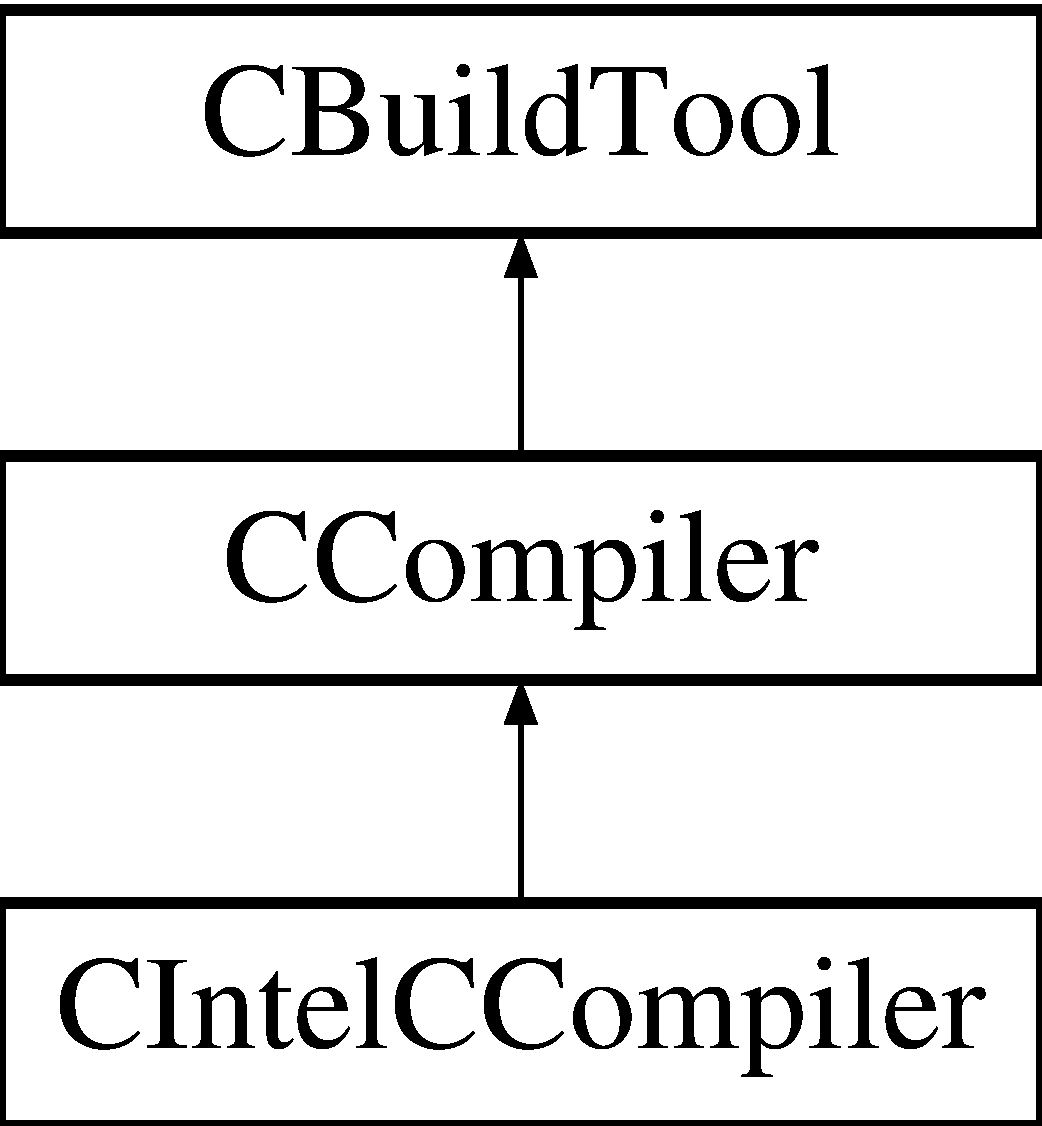
\includegraphics[height=3.000000cm]{d1/d74/classCIntelCCompiler}
\end{center}
\end{figure}
\subsection*{Public Member Functions}
\begin{DoxyCompactItemize}
\item 
virtual \hyperlink{classCIncludeSearchFilter}{C\-Include\-Search\-Filter} $\ast$ \hyperlink{classCIntelCCompiler_a1864ae37aea1eecddfcec8ab456dc8a3}{Include\-Search\-Filter} (void) const 
\item 
virtual \hyperlink{classCIntelCCompiler}{C\-Intel\-C\-Compiler} $\ast$ \hyperlink{classCIntelCCompiler_a4f259da4011feabc53b1ebf9a26bd2de}{Create\-Instance} (void)
\item 
virtual void \hyperlink{classCIntelCCompiler_af5d140834df595d4b5e370e534acb933}{Reset} (const \hyperlink{classCPlatform_a2fb735c63c53052f79629e338bb0f535}{C\-Platform\-::\-O\-S\-\_\-\-Type} O\-S)
\item 
\hyperlink{classCIntelCCompiler_a5cc83d2a7e47dfe79bd132d616f950b7}{C\-Intel\-C\-Compiler} (void)
\end{DoxyCompactItemize}
\subsection*{Private Attributes}
\begin{DoxyCompactItemize}
\item 
\hyperlink{classCCppIncludeSearchFilter}{C\-Cpp\-Include\-Search\-Filter} \hyperlink{classCIntelCCompiler_a8c22765da736a3390cf467c94a86939c}{m\-\_\-\-Include\-Search\-Filter}
\end{DoxyCompactItemize}
\subsection*{Additional Inherited Members}


\subsection{Constructor \& Destructor Documentation}
\hypertarget{classCIntelCCompiler_a5cc83d2a7e47dfe79bd132d616f950b7}{\index{C\-Intel\-C\-Compiler@{C\-Intel\-C\-Compiler}!C\-Intel\-C\-Compiler@{C\-Intel\-C\-Compiler}}
\index{C\-Intel\-C\-Compiler@{C\-Intel\-C\-Compiler}!CIntelCCompiler@{C\-Intel\-C\-Compiler}}
\subsubsection[{C\-Intel\-C\-Compiler}]{\setlength{\rightskip}{0pt plus 5cm}C\-Intel\-C\-Compiler\-::\-C\-Intel\-C\-Compiler (
\begin{DoxyParamCaption}
\item[{void}]{}
\end{DoxyParamCaption}
)}}\label{classCIntelCCompiler_a5cc83d2a7e47dfe79bd132d616f950b7}


\subsection{Member Function Documentation}
\hypertarget{classCIntelCCompiler_a4f259da4011feabc53b1ebf9a26bd2de}{\index{C\-Intel\-C\-Compiler@{C\-Intel\-C\-Compiler}!Create\-Instance@{Create\-Instance}}
\index{Create\-Instance@{Create\-Instance}!CIntelCCompiler@{C\-Intel\-C\-Compiler}}
\subsubsection[{Create\-Instance}]{\setlength{\rightskip}{0pt plus 5cm}{\bf C\-Intel\-C\-Compiler} $\ast$ C\-Intel\-C\-Compiler\-::\-Create\-Instance (
\begin{DoxyParamCaption}
\item[{void}]{}
\end{DoxyParamCaption}
)\hspace{0.3cm}{\ttfamily [virtual]}}}\label{classCIntelCCompiler_a4f259da4011feabc53b1ebf9a26bd2de}


Reimplemented from \hyperlink{classCCompiler_a3d4aaaf69e1ba6070c729fd042d90012}{C\-Compiler}.

\hypertarget{classCIntelCCompiler_a1864ae37aea1eecddfcec8ab456dc8a3}{\index{C\-Intel\-C\-Compiler@{C\-Intel\-C\-Compiler}!Include\-Search\-Filter@{Include\-Search\-Filter}}
\index{Include\-Search\-Filter@{Include\-Search\-Filter}!CIntelCCompiler@{C\-Intel\-C\-Compiler}}
\subsubsection[{Include\-Search\-Filter}]{\setlength{\rightskip}{0pt plus 5cm}{\bf C\-Include\-Search\-Filter} $\ast$ C\-Intel\-C\-Compiler\-::\-Include\-Search\-Filter (
\begin{DoxyParamCaption}
\item[{void}]{}
\end{DoxyParamCaption}
) const\hspace{0.3cm}{\ttfamily [virtual]}}}\label{classCIntelCCompiler_a1864ae37aea1eecddfcec8ab456dc8a3}


Reimplemented from \hyperlink{classCCompiler_a1dc477f47e953ddd4c653f3ba85c5468}{C\-Compiler}.

\hypertarget{classCIntelCCompiler_af5d140834df595d4b5e370e534acb933}{\index{C\-Intel\-C\-Compiler@{C\-Intel\-C\-Compiler}!Reset@{Reset}}
\index{Reset@{Reset}!CIntelCCompiler@{C\-Intel\-C\-Compiler}}
\subsubsection[{Reset}]{\setlength{\rightskip}{0pt plus 5cm}void C\-Intel\-C\-Compiler\-::\-Reset (
\begin{DoxyParamCaption}
\item[{const {\bf C\-Platform\-::\-O\-S\-\_\-\-Type}}]{O\-S}
\end{DoxyParamCaption}
)\hspace{0.3cm}{\ttfamily [virtual]}}}\label{classCIntelCCompiler_af5d140834df595d4b5e370e534acb933}


Reimplemented from \hyperlink{classCBuildTool_abea21a0e61ab2177effdff5aaa169585}{C\-Build\-Tool}.



\subsection{Member Data Documentation}
\hypertarget{classCIntelCCompiler_a8c22765da736a3390cf467c94a86939c}{\index{C\-Intel\-C\-Compiler@{C\-Intel\-C\-Compiler}!m\-\_\-\-Include\-Search\-Filter@{m\-\_\-\-Include\-Search\-Filter}}
\index{m\-\_\-\-Include\-Search\-Filter@{m\-\_\-\-Include\-Search\-Filter}!CIntelCCompiler@{C\-Intel\-C\-Compiler}}
\subsubsection[{m\-\_\-\-Include\-Search\-Filter}]{\setlength{\rightskip}{0pt plus 5cm}{\bf C\-Cpp\-Include\-Search\-Filter} C\-Intel\-C\-Compiler\-::m\-\_\-\-Include\-Search\-Filter\hspace{0.3cm}{\ttfamily [private]}}}\label{classCIntelCCompiler_a8c22765da736a3390cf467c94a86939c}


The documentation for this class was generated from the following files\-:\begin{DoxyCompactItemize}
\item 
src/\hyperlink{buildtools_8h}{buildtools.\-h}\item 
src/\hyperlink{buildtools_8cpp}{buildtools.\-cpp}\end{DoxyCompactItemize}

\hypertarget{classCIntelCppCompiler}{\section{C\-Intel\-Cpp\-Compiler Class Reference}
\label{classCIntelCppCompiler}\index{C\-Intel\-Cpp\-Compiler@{C\-Intel\-Cpp\-Compiler}}
}


{\ttfamily \#include $<$buildtools.\-h$>$}

Inheritance diagram for C\-Intel\-Cpp\-Compiler\-:\begin{figure}[H]
\begin{center}
\leavevmode
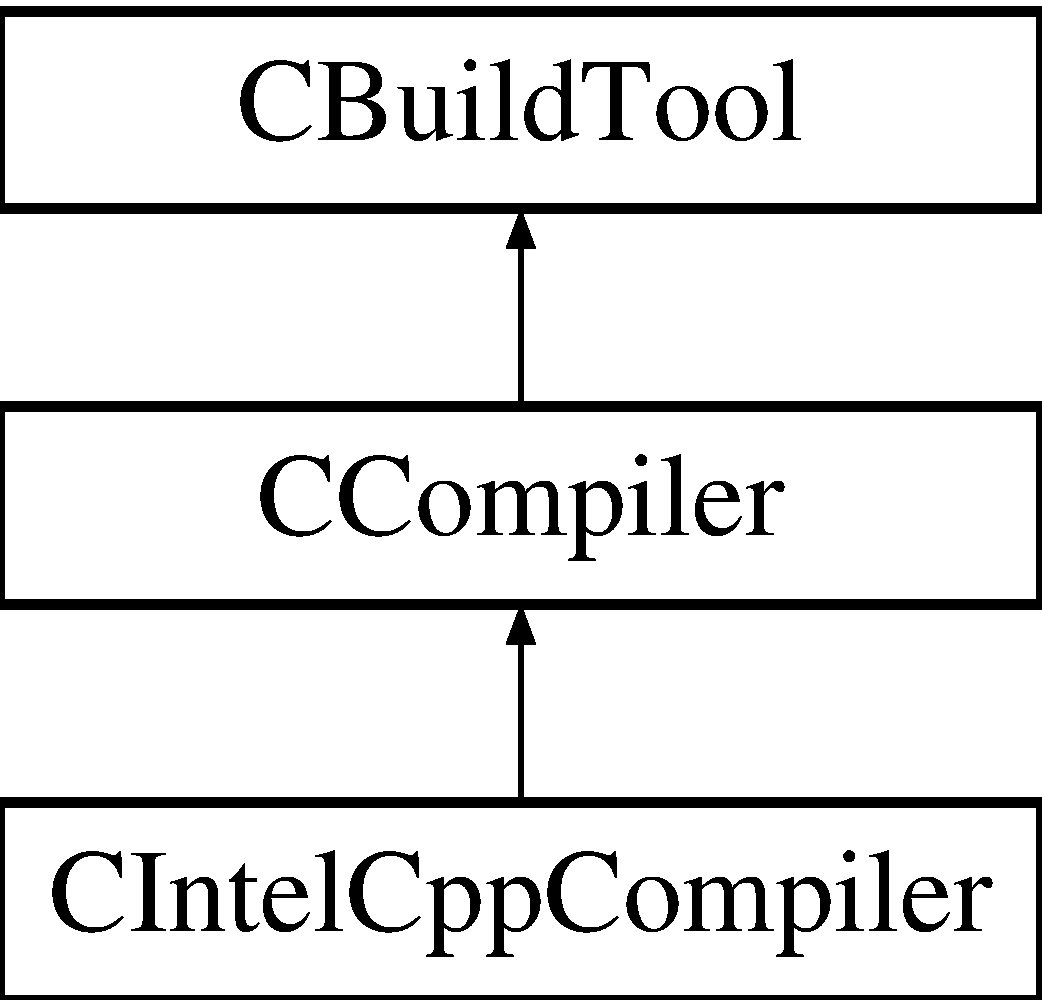
\includegraphics[height=3.000000cm]{dd/da0/classCIntelCppCompiler}
\end{center}
\end{figure}
\subsection*{Public Member Functions}
\begin{DoxyCompactItemize}
\item 
virtual \hyperlink{classCIncludeSearchFilter}{C\-Include\-Search\-Filter} $\ast$ \hyperlink{classCIntelCppCompiler_a7937ce18c293da16161f14e51d873b5a}{Include\-Search\-Filter} (void) const 
\item 
virtual \hyperlink{classCIntelCppCompiler}{C\-Intel\-Cpp\-Compiler} $\ast$ \hyperlink{classCIntelCppCompiler_a2e75b0ac5a7860128f25f29698f51509}{Create\-Instance} (void)
\item 
virtual void \hyperlink{classCIntelCppCompiler_a39338f5aead731a4fc834605d2d60c37}{Reset} (const \hyperlink{classCPlatform_a2fb735c63c53052f79629e338bb0f535}{C\-Platform\-::\-O\-S\-\_\-\-Type} O\-S)
\item 
\hyperlink{classCIntelCppCompiler_aa1a3357afdec8931fc7e17ebc317a1e6}{C\-Intel\-Cpp\-Compiler} (void)
\end{DoxyCompactItemize}
\subsection*{Private Attributes}
\begin{DoxyCompactItemize}
\item 
\hyperlink{classCCppIncludeSearchFilter}{C\-Cpp\-Include\-Search\-Filter} \hyperlink{classCIntelCppCompiler_a3d70f7d935b38d79cec20db5f387071f}{m\-\_\-\-Include\-Search\-Filter}
\end{DoxyCompactItemize}
\subsection*{Additional Inherited Members}


\subsection{Constructor \& Destructor Documentation}
\hypertarget{classCIntelCppCompiler_aa1a3357afdec8931fc7e17ebc317a1e6}{\index{C\-Intel\-Cpp\-Compiler@{C\-Intel\-Cpp\-Compiler}!C\-Intel\-Cpp\-Compiler@{C\-Intel\-Cpp\-Compiler}}
\index{C\-Intel\-Cpp\-Compiler@{C\-Intel\-Cpp\-Compiler}!CIntelCppCompiler@{C\-Intel\-Cpp\-Compiler}}
\subsubsection[{C\-Intel\-Cpp\-Compiler}]{\setlength{\rightskip}{0pt plus 5cm}C\-Intel\-Cpp\-Compiler\-::\-C\-Intel\-Cpp\-Compiler (
\begin{DoxyParamCaption}
\item[{void}]{}
\end{DoxyParamCaption}
)}}\label{classCIntelCppCompiler_aa1a3357afdec8931fc7e17ebc317a1e6}


\subsection{Member Function Documentation}
\hypertarget{classCIntelCppCompiler_a2e75b0ac5a7860128f25f29698f51509}{\index{C\-Intel\-Cpp\-Compiler@{C\-Intel\-Cpp\-Compiler}!Create\-Instance@{Create\-Instance}}
\index{Create\-Instance@{Create\-Instance}!CIntelCppCompiler@{C\-Intel\-Cpp\-Compiler}}
\subsubsection[{Create\-Instance}]{\setlength{\rightskip}{0pt plus 5cm}{\bf C\-Intel\-Cpp\-Compiler} $\ast$ C\-Intel\-Cpp\-Compiler\-::\-Create\-Instance (
\begin{DoxyParamCaption}
\item[{void}]{}
\end{DoxyParamCaption}
)\hspace{0.3cm}{\ttfamily [virtual]}}}\label{classCIntelCppCompiler_a2e75b0ac5a7860128f25f29698f51509}


Reimplemented from \hyperlink{classCCompiler_a3d4aaaf69e1ba6070c729fd042d90012}{C\-Compiler}.

\hypertarget{classCIntelCppCompiler_a7937ce18c293da16161f14e51d873b5a}{\index{C\-Intel\-Cpp\-Compiler@{C\-Intel\-Cpp\-Compiler}!Include\-Search\-Filter@{Include\-Search\-Filter}}
\index{Include\-Search\-Filter@{Include\-Search\-Filter}!CIntelCppCompiler@{C\-Intel\-Cpp\-Compiler}}
\subsubsection[{Include\-Search\-Filter}]{\setlength{\rightskip}{0pt plus 5cm}{\bf C\-Include\-Search\-Filter} $\ast$ C\-Intel\-Cpp\-Compiler\-::\-Include\-Search\-Filter (
\begin{DoxyParamCaption}
\item[{void}]{}
\end{DoxyParamCaption}
) const\hspace{0.3cm}{\ttfamily [virtual]}}}\label{classCIntelCppCompiler_a7937ce18c293da16161f14e51d873b5a}


Reimplemented from \hyperlink{classCCompiler_a1dc477f47e953ddd4c653f3ba85c5468}{C\-Compiler}.

\hypertarget{classCIntelCppCompiler_a39338f5aead731a4fc834605d2d60c37}{\index{C\-Intel\-Cpp\-Compiler@{C\-Intel\-Cpp\-Compiler}!Reset@{Reset}}
\index{Reset@{Reset}!CIntelCppCompiler@{C\-Intel\-Cpp\-Compiler}}
\subsubsection[{Reset}]{\setlength{\rightskip}{0pt plus 5cm}void C\-Intel\-Cpp\-Compiler\-::\-Reset (
\begin{DoxyParamCaption}
\item[{const {\bf C\-Platform\-::\-O\-S\-\_\-\-Type}}]{O\-S}
\end{DoxyParamCaption}
)\hspace{0.3cm}{\ttfamily [virtual]}}}\label{classCIntelCppCompiler_a39338f5aead731a4fc834605d2d60c37}


Reimplemented from \hyperlink{classCBuildTool_abea21a0e61ab2177effdff5aaa169585}{C\-Build\-Tool}.



\subsection{Member Data Documentation}
\hypertarget{classCIntelCppCompiler_a3d70f7d935b38d79cec20db5f387071f}{\index{C\-Intel\-Cpp\-Compiler@{C\-Intel\-Cpp\-Compiler}!m\-\_\-\-Include\-Search\-Filter@{m\-\_\-\-Include\-Search\-Filter}}
\index{m\-\_\-\-Include\-Search\-Filter@{m\-\_\-\-Include\-Search\-Filter}!CIntelCppCompiler@{C\-Intel\-Cpp\-Compiler}}
\subsubsection[{m\-\_\-\-Include\-Search\-Filter}]{\setlength{\rightskip}{0pt plus 5cm}{\bf C\-Cpp\-Include\-Search\-Filter} C\-Intel\-Cpp\-Compiler\-::m\-\_\-\-Include\-Search\-Filter\hspace{0.3cm}{\ttfamily [private]}}}\label{classCIntelCppCompiler_a3d70f7d935b38d79cec20db5f387071f}


The documentation for this class was generated from the following files\-:\begin{DoxyCompactItemize}
\item 
src/\hyperlink{buildtools_8h}{buildtools.\-h}\item 
src/\hyperlink{buildtools_8cpp}{buildtools.\-cpp}\end{DoxyCompactItemize}

\hypertarget{classCIntelDynamicLinker}{\section{C\-Intel\-Dynamic\-Linker Class Reference}
\label{classCIntelDynamicLinker}\index{C\-Intel\-Dynamic\-Linker@{C\-Intel\-Dynamic\-Linker}}
}


{\ttfamily \#include $<$buildtools.\-h$>$}

Inheritance diagram for C\-Intel\-Dynamic\-Linker\-:\begin{figure}[H]
\begin{center}
\leavevmode
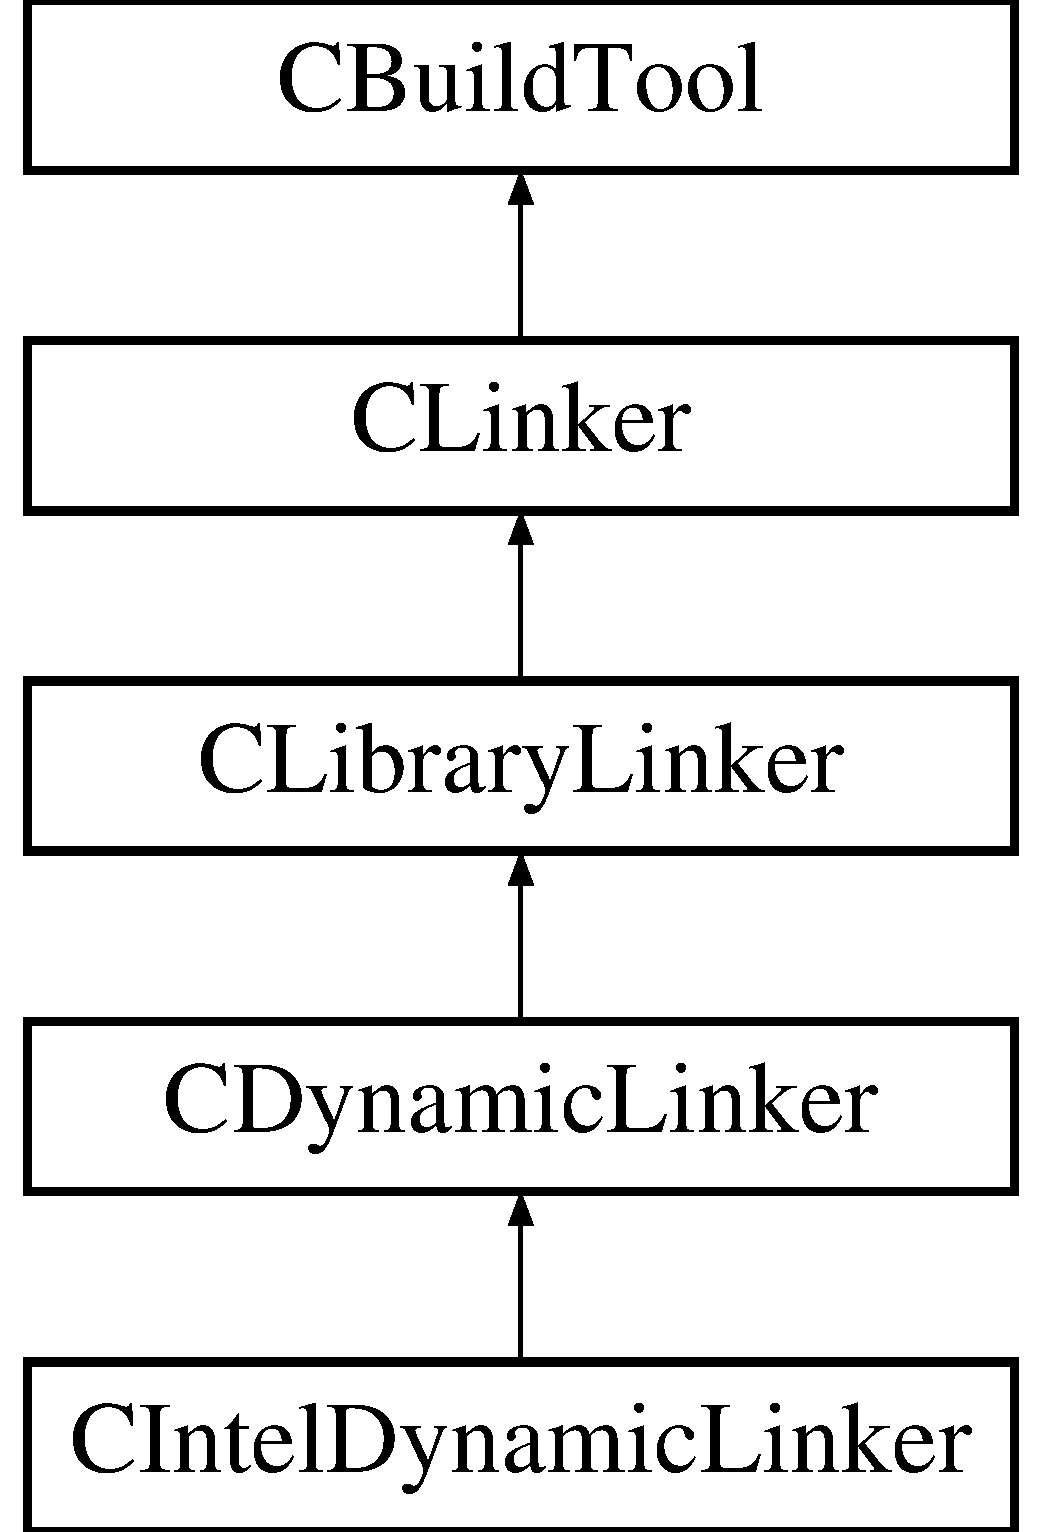
\includegraphics[height=5.000000cm]{df/d46/classCIntelDynamicLinker}
\end{center}
\end{figure}
\subsection*{Public Member Functions}
\begin{DoxyCompactItemize}
\item 
virtual \hyperlink{classCIntelDynamicLinker}{C\-Intel\-Dynamic\-Linker} $\ast$ \hyperlink{classCIntelDynamicLinker_a51e4c22985b5c518e8cdef1abeee7d85}{Create\-Instance} (void)
\item 
virtual void \hyperlink{classCIntelDynamicLinker_a9716e2053535fcadd92d46699d8b445e}{Reset} (const \hyperlink{classCPlatform_a2fb735c63c53052f79629e338bb0f535}{C\-Platform\-::\-O\-S\-\_\-\-Type} O\-S)
\item 
\hyperlink{classCIntelDynamicLinker_a2cc50760a8790598abf18d2e28659ace}{C\-Intel\-Dynamic\-Linker} (void)
\end{DoxyCompactItemize}
\subsection*{Additional Inherited Members}


\subsection{Constructor \& Destructor Documentation}
\hypertarget{classCIntelDynamicLinker_a2cc50760a8790598abf18d2e28659ace}{\index{C\-Intel\-Dynamic\-Linker@{C\-Intel\-Dynamic\-Linker}!C\-Intel\-Dynamic\-Linker@{C\-Intel\-Dynamic\-Linker}}
\index{C\-Intel\-Dynamic\-Linker@{C\-Intel\-Dynamic\-Linker}!CIntelDynamicLinker@{C\-Intel\-Dynamic\-Linker}}
\subsubsection[{C\-Intel\-Dynamic\-Linker}]{\setlength{\rightskip}{0pt plus 5cm}C\-Intel\-Dynamic\-Linker\-::\-C\-Intel\-Dynamic\-Linker (
\begin{DoxyParamCaption}
\item[{void}]{}
\end{DoxyParamCaption}
)}}\label{classCIntelDynamicLinker_a2cc50760a8790598abf18d2e28659ace}


\subsection{Member Function Documentation}
\hypertarget{classCIntelDynamicLinker_a51e4c22985b5c518e8cdef1abeee7d85}{\index{C\-Intel\-Dynamic\-Linker@{C\-Intel\-Dynamic\-Linker}!Create\-Instance@{Create\-Instance}}
\index{Create\-Instance@{Create\-Instance}!CIntelDynamicLinker@{C\-Intel\-Dynamic\-Linker}}
\subsubsection[{Create\-Instance}]{\setlength{\rightskip}{0pt plus 5cm}{\bf C\-Intel\-Dynamic\-Linker} $\ast$ C\-Intel\-Dynamic\-Linker\-::\-Create\-Instance (
\begin{DoxyParamCaption}
\item[{void}]{}
\end{DoxyParamCaption}
)\hspace{0.3cm}{\ttfamily [virtual]}}}\label{classCIntelDynamicLinker_a51e4c22985b5c518e8cdef1abeee7d85}


Reimplemented from \hyperlink{classCDynamicLinker_ac71406ca5c6e8e991a6418a6307d274c}{C\-Dynamic\-Linker}.

\hypertarget{classCIntelDynamicLinker_a9716e2053535fcadd92d46699d8b445e}{\index{C\-Intel\-Dynamic\-Linker@{C\-Intel\-Dynamic\-Linker}!Reset@{Reset}}
\index{Reset@{Reset}!CIntelDynamicLinker@{C\-Intel\-Dynamic\-Linker}}
\subsubsection[{Reset}]{\setlength{\rightskip}{0pt plus 5cm}void C\-Intel\-Dynamic\-Linker\-::\-Reset (
\begin{DoxyParamCaption}
\item[{const {\bf C\-Platform\-::\-O\-S\-\_\-\-Type}}]{O\-S}
\end{DoxyParamCaption}
)\hspace{0.3cm}{\ttfamily [virtual]}}}\label{classCIntelDynamicLinker_a9716e2053535fcadd92d46699d8b445e}


Reimplemented from \hyperlink{classCDynamicLinker_a437d46ee65b3585e7be9d15d40c26820}{C\-Dynamic\-Linker}.



The documentation for this class was generated from the following files\-:\begin{DoxyCompactItemize}
\item 
src/\hyperlink{buildtools_8h}{buildtools.\-h}\item 
src/\hyperlink{buildtools_8cpp}{buildtools.\-cpp}\end{DoxyCompactItemize}

\hypertarget{classCIntelExecutableLinker}{\section{C\-Intel\-Executable\-Linker Class Reference}
\label{classCIntelExecutableLinker}\index{C\-Intel\-Executable\-Linker@{C\-Intel\-Executable\-Linker}}
}


{\ttfamily \#include $<$buildtools.\-h$>$}

Inheritance diagram for C\-Intel\-Executable\-Linker\-:\begin{figure}[H]
\begin{center}
\leavevmode
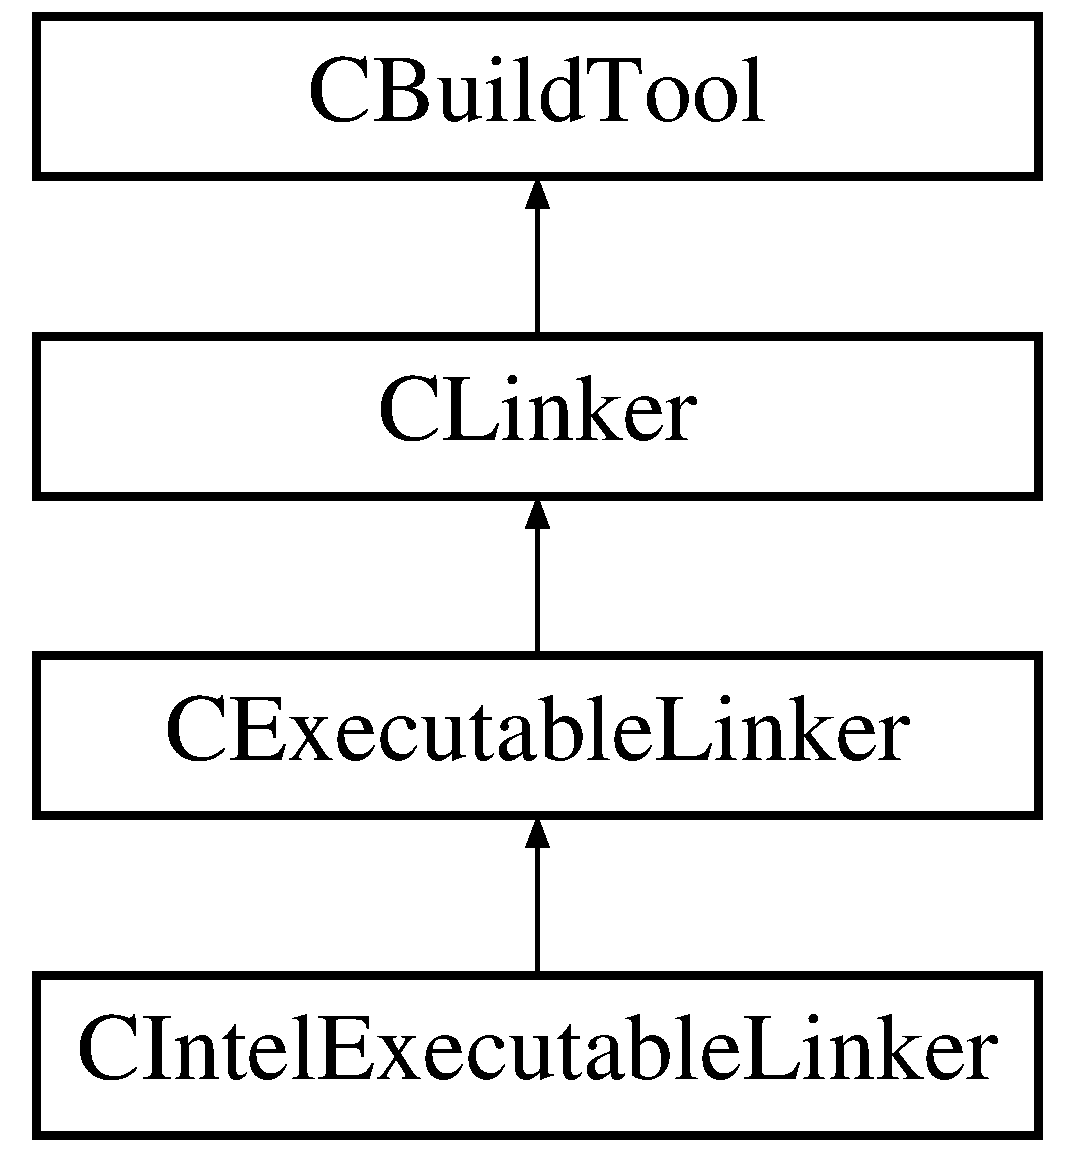
\includegraphics[height=4.000000cm]{d9/d5f/classCIntelExecutableLinker}
\end{center}
\end{figure}
\subsection*{Public Member Functions}
\begin{DoxyCompactItemize}
\item 
virtual \hyperlink{classCIntelExecutableLinker}{C\-Intel\-Executable\-Linker} $\ast$ \hyperlink{classCIntelExecutableLinker_aacec1bc57c88a614c449a6873c1cc489}{Create\-Instance} (void)
\item 
virtual void \hyperlink{classCIntelExecutableLinker_adb14460fc50fb8d0e7ef29fd991d4271}{Reset} (const \hyperlink{classCPlatform_a2fb735c63c53052f79629e338bb0f535}{C\-Platform\-::\-O\-S\-\_\-\-Type} O\-S)
\item 
\hyperlink{classCIntelExecutableLinker_ab4e0500d893ba46ca154c191f9e20e3c}{C\-Intel\-Executable\-Linker} (void)
\end{DoxyCompactItemize}
\subsection*{Additional Inherited Members}


\subsection{Constructor \& Destructor Documentation}
\hypertarget{classCIntelExecutableLinker_ab4e0500d893ba46ca154c191f9e20e3c}{\index{C\-Intel\-Executable\-Linker@{C\-Intel\-Executable\-Linker}!C\-Intel\-Executable\-Linker@{C\-Intel\-Executable\-Linker}}
\index{C\-Intel\-Executable\-Linker@{C\-Intel\-Executable\-Linker}!CIntelExecutableLinker@{C\-Intel\-Executable\-Linker}}
\subsubsection[{C\-Intel\-Executable\-Linker}]{\setlength{\rightskip}{0pt plus 5cm}C\-Intel\-Executable\-Linker\-::\-C\-Intel\-Executable\-Linker (
\begin{DoxyParamCaption}
\item[{void}]{}
\end{DoxyParamCaption}
)}}\label{classCIntelExecutableLinker_ab4e0500d893ba46ca154c191f9e20e3c}


\subsection{Member Function Documentation}
\hypertarget{classCIntelExecutableLinker_aacec1bc57c88a614c449a6873c1cc489}{\index{C\-Intel\-Executable\-Linker@{C\-Intel\-Executable\-Linker}!Create\-Instance@{Create\-Instance}}
\index{Create\-Instance@{Create\-Instance}!CIntelExecutableLinker@{C\-Intel\-Executable\-Linker}}
\subsubsection[{Create\-Instance}]{\setlength{\rightskip}{0pt plus 5cm}{\bf C\-Intel\-Executable\-Linker} $\ast$ C\-Intel\-Executable\-Linker\-::\-Create\-Instance (
\begin{DoxyParamCaption}
\item[{void}]{}
\end{DoxyParamCaption}
)\hspace{0.3cm}{\ttfamily [virtual]}}}\label{classCIntelExecutableLinker_aacec1bc57c88a614c449a6873c1cc489}


Reimplemented from \hyperlink{classCExecutableLinker_a457b823b737b0a78285d5ede77df827c}{C\-Executable\-Linker}.

\hypertarget{classCIntelExecutableLinker_adb14460fc50fb8d0e7ef29fd991d4271}{\index{C\-Intel\-Executable\-Linker@{C\-Intel\-Executable\-Linker}!Reset@{Reset}}
\index{Reset@{Reset}!CIntelExecutableLinker@{C\-Intel\-Executable\-Linker}}
\subsubsection[{Reset}]{\setlength{\rightskip}{0pt plus 5cm}void C\-Intel\-Executable\-Linker\-::\-Reset (
\begin{DoxyParamCaption}
\item[{const {\bf C\-Platform\-::\-O\-S\-\_\-\-Type}}]{O\-S}
\end{DoxyParamCaption}
)\hspace{0.3cm}{\ttfamily [virtual]}}}\label{classCIntelExecutableLinker_adb14460fc50fb8d0e7ef29fd991d4271}


Reimplemented from \hyperlink{classCBuildTool_abea21a0e61ab2177effdff5aaa169585}{C\-Build\-Tool}.



The documentation for this class was generated from the following files\-:\begin{DoxyCompactItemize}
\item 
src/\hyperlink{buildtools_8h}{buildtools.\-h}\item 
src/\hyperlink{buildtools_8cpp}{buildtools.\-cpp}\end{DoxyCompactItemize}

\hypertarget{classCIntelStaticLinker}{\section{C\-Intel\-Static\-Linker Class Reference}
\label{classCIntelStaticLinker}\index{C\-Intel\-Static\-Linker@{C\-Intel\-Static\-Linker}}
}


{\ttfamily \#include $<$buildtools.\-h$>$}

Inheritance diagram for C\-Intel\-Static\-Linker\-:\begin{figure}[H]
\begin{center}
\leavevmode
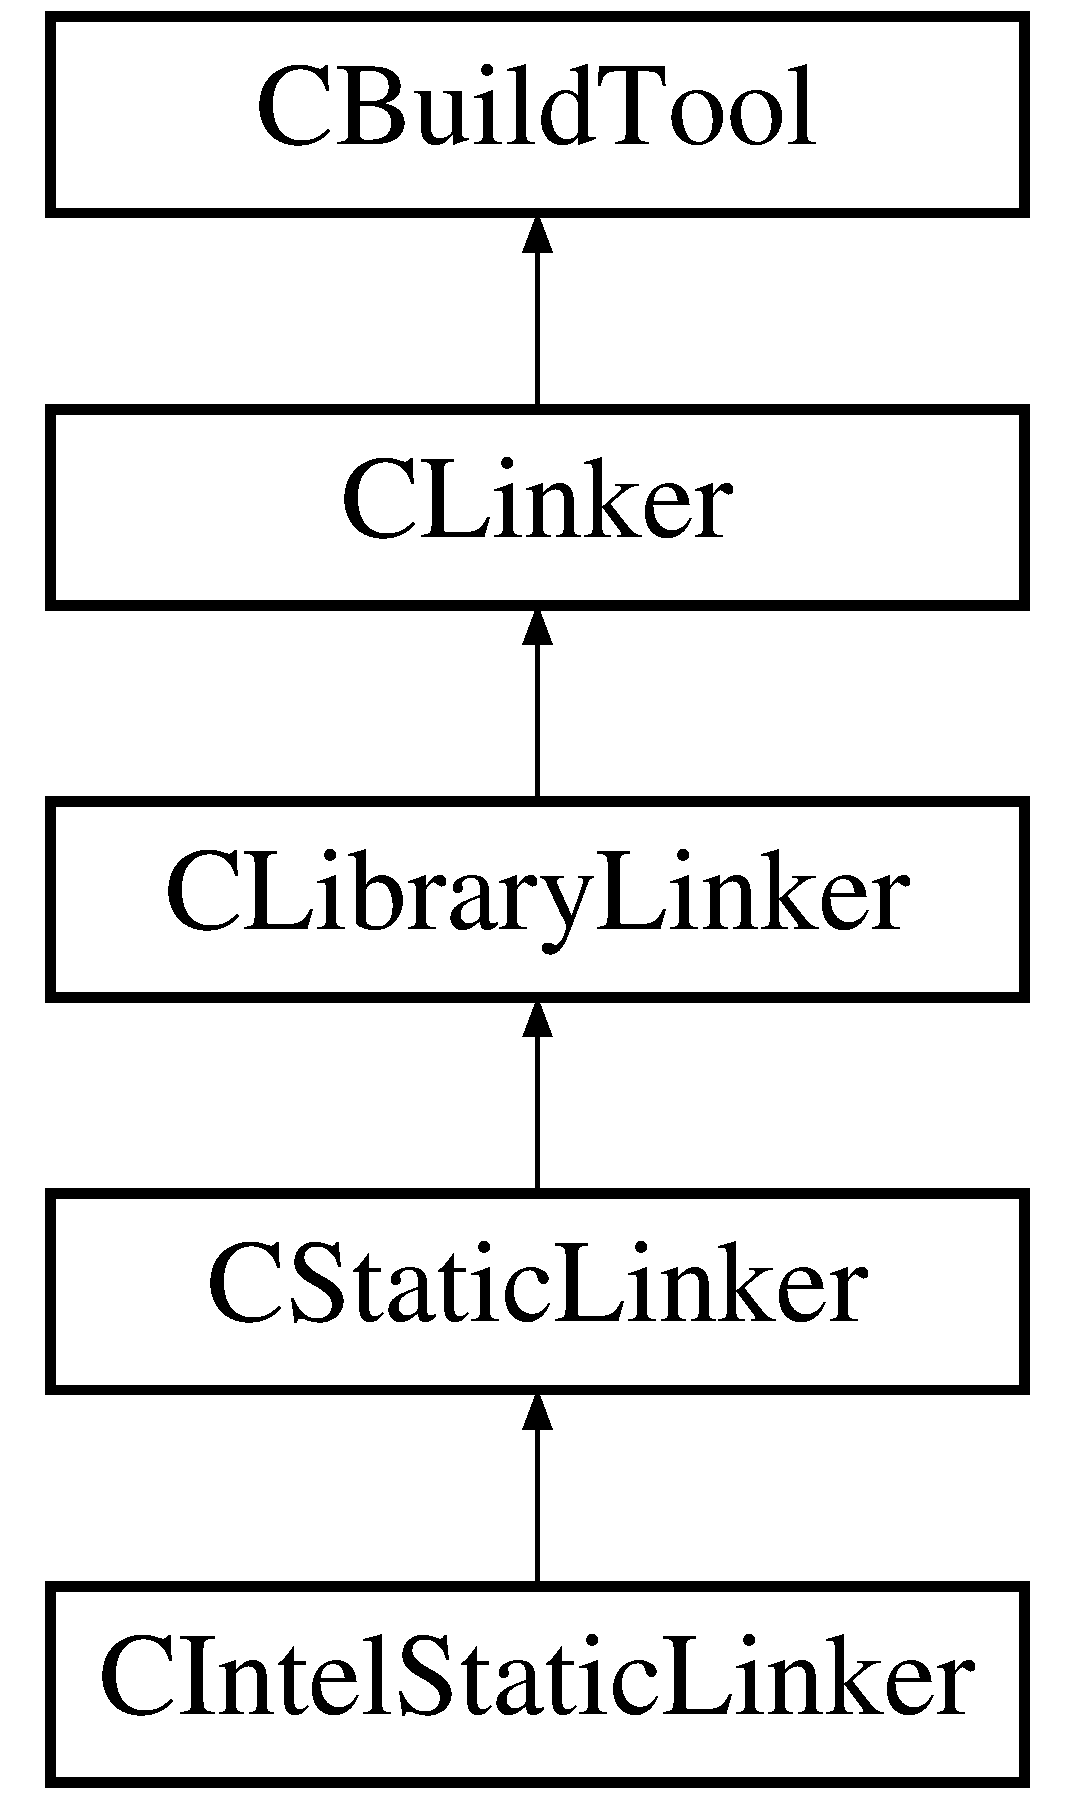
\includegraphics[height=5.000000cm]{db/dc9/classCIntelStaticLinker}
\end{center}
\end{figure}
\subsection*{Public Member Functions}
\begin{DoxyCompactItemize}
\item 
virtual \hyperlink{classCIntelStaticLinker}{C\-Intel\-Static\-Linker} $\ast$ \hyperlink{classCIntelStaticLinker_af5e68a1b09bc64dd30af6d7e9ffe6266}{Create\-Instance} (void)
\item 
virtual void \hyperlink{classCIntelStaticLinker_a71064c1a78086c73ddae37f4ecf513c2}{Reset} (const \hyperlink{classCPlatform_a2fb735c63c53052f79629e338bb0f535}{C\-Platform\-::\-O\-S\-\_\-\-Type} O\-S)
\item 
\hyperlink{classCIntelStaticLinker_a24911cbc0e3aea0ee567a4736da819ce}{C\-Intel\-Static\-Linker} (void)
\end{DoxyCompactItemize}
\subsection*{Additional Inherited Members}


\subsection{Constructor \& Destructor Documentation}
\hypertarget{classCIntelStaticLinker_a24911cbc0e3aea0ee567a4736da819ce}{\index{C\-Intel\-Static\-Linker@{C\-Intel\-Static\-Linker}!C\-Intel\-Static\-Linker@{C\-Intel\-Static\-Linker}}
\index{C\-Intel\-Static\-Linker@{C\-Intel\-Static\-Linker}!CIntelStaticLinker@{C\-Intel\-Static\-Linker}}
\subsubsection[{C\-Intel\-Static\-Linker}]{\setlength{\rightskip}{0pt plus 5cm}C\-Intel\-Static\-Linker\-::\-C\-Intel\-Static\-Linker (
\begin{DoxyParamCaption}
\item[{void}]{}
\end{DoxyParamCaption}
)}}\label{classCIntelStaticLinker_a24911cbc0e3aea0ee567a4736da819ce}


\subsection{Member Function Documentation}
\hypertarget{classCIntelStaticLinker_af5e68a1b09bc64dd30af6d7e9ffe6266}{\index{C\-Intel\-Static\-Linker@{C\-Intel\-Static\-Linker}!Create\-Instance@{Create\-Instance}}
\index{Create\-Instance@{Create\-Instance}!CIntelStaticLinker@{C\-Intel\-Static\-Linker}}
\subsubsection[{Create\-Instance}]{\setlength{\rightskip}{0pt plus 5cm}{\bf C\-Intel\-Static\-Linker} $\ast$ C\-Intel\-Static\-Linker\-::\-Create\-Instance (
\begin{DoxyParamCaption}
\item[{void}]{}
\end{DoxyParamCaption}
)\hspace{0.3cm}{\ttfamily [virtual]}}}\label{classCIntelStaticLinker_af5e68a1b09bc64dd30af6d7e9ffe6266}


Reimplemented from \hyperlink{classCStaticLinker_a7e626491caa847ef207032ee600625db}{C\-Static\-Linker}.

\hypertarget{classCIntelStaticLinker_a71064c1a78086c73ddae37f4ecf513c2}{\index{C\-Intel\-Static\-Linker@{C\-Intel\-Static\-Linker}!Reset@{Reset}}
\index{Reset@{Reset}!CIntelStaticLinker@{C\-Intel\-Static\-Linker}}
\subsubsection[{Reset}]{\setlength{\rightskip}{0pt plus 5cm}void C\-Intel\-Static\-Linker\-::\-Reset (
\begin{DoxyParamCaption}
\item[{const {\bf C\-Platform\-::\-O\-S\-\_\-\-Type}}]{O\-S}
\end{DoxyParamCaption}
)\hspace{0.3cm}{\ttfamily [virtual]}}}\label{classCIntelStaticLinker_a71064c1a78086c73ddae37f4ecf513c2}


Reimplemented from \hyperlink{classCBuildTool_abea21a0e61ab2177effdff5aaa169585}{C\-Build\-Tool}.



The documentation for this class was generated from the following files\-:\begin{DoxyCompactItemize}
\item 
src/\hyperlink{buildtools_8h}{buildtools.\-h}\item 
src/\hyperlink{buildtools_8cpp}{buildtools.\-cpp}\end{DoxyCompactItemize}

\hypertarget{classCIntelToolChain}{\section{C\-Intel\-Tool\-Chain Class Reference}
\label{classCIntelToolChain}\index{C\-Intel\-Tool\-Chain@{C\-Intel\-Tool\-Chain}}
}


{\ttfamily \#include $<$toolchains.\-h$>$}

Inheritance diagram for C\-Intel\-Tool\-Chain\-:\begin{figure}[H]
\begin{center}
\leavevmode
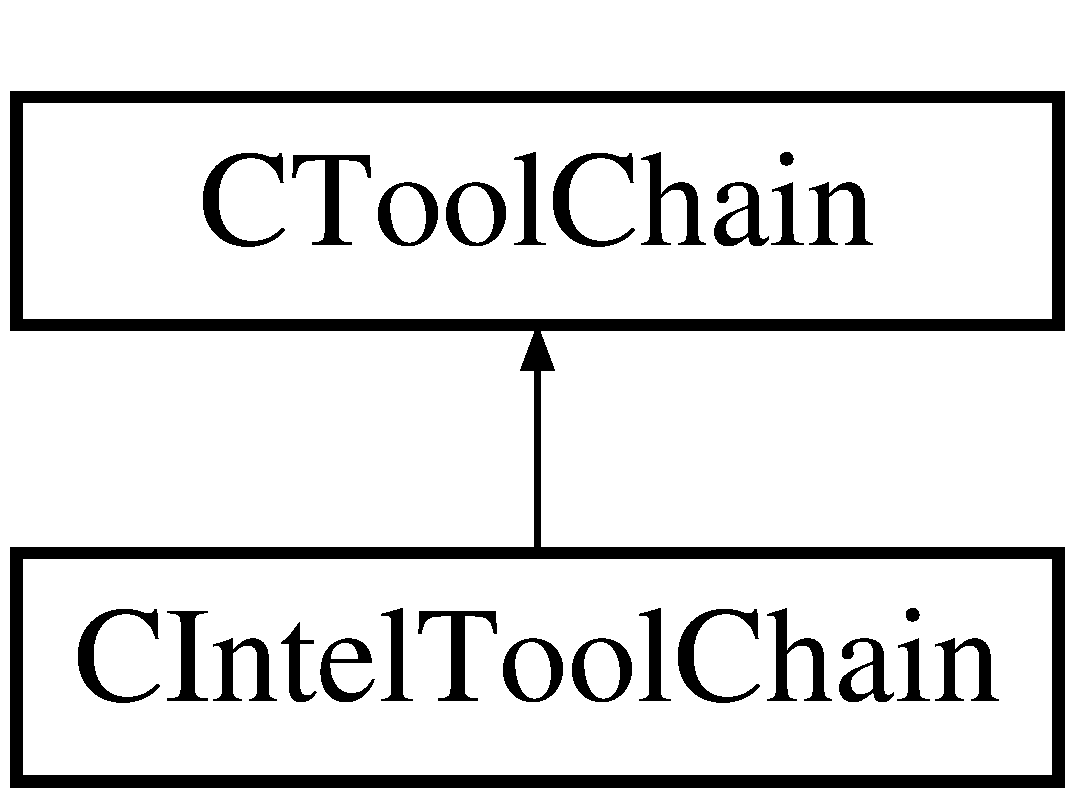
\includegraphics[height=2.000000cm]{db/dbe/classCIntelToolChain}
\end{center}
\end{figure}
\subsection*{Public Member Functions}
\begin{DoxyCompactItemize}
\item 
virtual \hyperlink{classCToolChain}{C\-Tool\-Chain} $\ast$ \hyperlink{classCIntelToolChain_a75365a2d8de5733f902e47d07a93fe45}{Create\-Instance} (void) const 
\item 
virtual void \hyperlink{classCIntelToolChain_a96bed03faaf53341c0b046c7163c9705}{Reset} (const \hyperlink{classCPlatform_a2fb735c63c53052f79629e338bb0f535}{C\-Platform\-::\-O\-S\-\_\-\-Type} \hyperlink{classCToolChain_abe4054d9081351e099163e2c53b260f8}{O\-S})
\item 
\hyperlink{classCIntelToolChain_a70cb7ff6ede35c56ddc30dd53cdc80ca}{C\-Intel\-Tool\-Chain} (void)
\item 
virtual \hyperlink{classCIntelToolChain_ad8857b58405ee3a6d2f62dff68710927}{$\sim$\-C\-Intel\-Tool\-Chain} (void)
\end{DoxyCompactItemize}
\subsection*{Additional Inherited Members}


\subsection{Constructor \& Destructor Documentation}
\hypertarget{classCIntelToolChain_a70cb7ff6ede35c56ddc30dd53cdc80ca}{\index{C\-Intel\-Tool\-Chain@{C\-Intel\-Tool\-Chain}!C\-Intel\-Tool\-Chain@{C\-Intel\-Tool\-Chain}}
\index{C\-Intel\-Tool\-Chain@{C\-Intel\-Tool\-Chain}!CIntelToolChain@{C\-Intel\-Tool\-Chain}}
\subsubsection[{C\-Intel\-Tool\-Chain}]{\setlength{\rightskip}{0pt plus 5cm}C\-Intel\-Tool\-Chain\-::\-C\-Intel\-Tool\-Chain (
\begin{DoxyParamCaption}
\item[{void}]{}
\end{DoxyParamCaption}
)}}\label{classCIntelToolChain_a70cb7ff6ede35c56ddc30dd53cdc80ca}
\hypertarget{classCIntelToolChain_ad8857b58405ee3a6d2f62dff68710927}{\index{C\-Intel\-Tool\-Chain@{C\-Intel\-Tool\-Chain}!$\sim$\-C\-Intel\-Tool\-Chain@{$\sim$\-C\-Intel\-Tool\-Chain}}
\index{$\sim$\-C\-Intel\-Tool\-Chain@{$\sim$\-C\-Intel\-Tool\-Chain}!CIntelToolChain@{C\-Intel\-Tool\-Chain}}
\subsubsection[{$\sim$\-C\-Intel\-Tool\-Chain}]{\setlength{\rightskip}{0pt plus 5cm}C\-Intel\-Tool\-Chain\-::$\sim$\-C\-Intel\-Tool\-Chain (
\begin{DoxyParamCaption}
\item[{void}]{}
\end{DoxyParamCaption}
)\hspace{0.3cm}{\ttfamily [virtual]}}}\label{classCIntelToolChain_ad8857b58405ee3a6d2f62dff68710927}


\subsection{Member Function Documentation}
\hypertarget{classCIntelToolChain_a75365a2d8de5733f902e47d07a93fe45}{\index{C\-Intel\-Tool\-Chain@{C\-Intel\-Tool\-Chain}!Create\-Instance@{Create\-Instance}}
\index{Create\-Instance@{Create\-Instance}!CIntelToolChain@{C\-Intel\-Tool\-Chain}}
\subsubsection[{Create\-Instance}]{\setlength{\rightskip}{0pt plus 5cm}{\bf C\-Tool\-Chain} $\ast$ C\-Intel\-Tool\-Chain\-::\-Create\-Instance (
\begin{DoxyParamCaption}
\item[{void}]{}
\end{DoxyParamCaption}
) const\hspace{0.3cm}{\ttfamily [virtual]}}}\label{classCIntelToolChain_a75365a2d8de5733f902e47d07a93fe45}


Reimplemented from \hyperlink{classCToolChain_aa6765d5197d898efb01d032ac73b7764}{C\-Tool\-Chain}.

\hypertarget{classCIntelToolChain_a96bed03faaf53341c0b046c7163c9705}{\index{C\-Intel\-Tool\-Chain@{C\-Intel\-Tool\-Chain}!Reset@{Reset}}
\index{Reset@{Reset}!CIntelToolChain@{C\-Intel\-Tool\-Chain}}
\subsubsection[{Reset}]{\setlength{\rightskip}{0pt plus 5cm}void C\-Intel\-Tool\-Chain\-::\-Reset (
\begin{DoxyParamCaption}
\item[{const {\bf C\-Platform\-::\-O\-S\-\_\-\-Type}}]{O\-S}
\end{DoxyParamCaption}
)\hspace{0.3cm}{\ttfamily [virtual]}}}\label{classCIntelToolChain_a96bed03faaf53341c0b046c7163c9705}


Reimplemented from \hyperlink{classCToolChain_a3b48ddb23b898b3b6eaa356a2ed6fbf8}{C\-Tool\-Chain}.



The documentation for this class was generated from the following files\-:\begin{DoxyCompactItemize}
\item 
src/\hyperlink{toolchains_8h}{toolchains.\-h}\item 
src/\hyperlink{toolchains_8cpp}{toolchains.\-cpp}\end{DoxyCompactItemize}

\hypertarget{classCLibraryLinker}{\section{C\-Library\-Linker Class Reference}
\label{classCLibraryLinker}\index{C\-Library\-Linker@{C\-Library\-Linker}}
}


{\ttfamily \#include $<$buildtools.\-h$>$}

Inheritance diagram for C\-Library\-Linker\-:\begin{figure}[H]
\begin{center}
\leavevmode
\includegraphics[height=8.383233cm]{df/d43/classCLibraryLinker}
\end{center}
\end{figure}
\subsection*{Public Member Functions}
\begin{DoxyCompactItemize}
\item 
virtual \hyperlink{classCLibraryLinker}{C\-Library\-Linker} $\ast$ \hyperlink{classCLibraryLinker_a02b85c6bc81ad2973ee9a578412a1fa0}{Create\-Instance} (void)
\item 
\hyperlink{classCLibraryLinker_a7fc487106f71f171c15186d6335e3ab0}{C\-Library\-Linker} (void)
\item 
\hyperlink{classCLibraryLinker_a804803dde5295ef609179daf12dee48e}{C\-Library\-Linker} (const \hyperlink{classCLibraryLinker}{C\-Library\-Linker} \&Library\-Linker)
\item 
virtual \hyperlink{classCLibraryLinker_ac9de66fedc3e398fa69d413650b31510}{$\sim$\-C\-Library\-Linker} (void)
\end{DoxyCompactItemize}
\subsection*{Additional Inherited Members}


\subsection{Constructor \& Destructor Documentation}
\hypertarget{classCLibraryLinker_a7fc487106f71f171c15186d6335e3ab0}{\index{C\-Library\-Linker@{C\-Library\-Linker}!C\-Library\-Linker@{C\-Library\-Linker}}
\index{C\-Library\-Linker@{C\-Library\-Linker}!CLibraryLinker@{C\-Library\-Linker}}
\subsubsection[{C\-Library\-Linker}]{\setlength{\rightskip}{0pt plus 5cm}C\-Library\-Linker\-::\-C\-Library\-Linker (
\begin{DoxyParamCaption}
\item[{void}]{}
\end{DoxyParamCaption}
)}}\label{classCLibraryLinker_a7fc487106f71f171c15186d6335e3ab0}
\hypertarget{classCLibraryLinker_a804803dde5295ef609179daf12dee48e}{\index{C\-Library\-Linker@{C\-Library\-Linker}!C\-Library\-Linker@{C\-Library\-Linker}}
\index{C\-Library\-Linker@{C\-Library\-Linker}!CLibraryLinker@{C\-Library\-Linker}}
\subsubsection[{C\-Library\-Linker}]{\setlength{\rightskip}{0pt plus 5cm}C\-Library\-Linker\-::\-C\-Library\-Linker (
\begin{DoxyParamCaption}
\item[{const {\bf C\-Library\-Linker} \&}]{Library\-Linker}
\end{DoxyParamCaption}
)}}\label{classCLibraryLinker_a804803dde5295ef609179daf12dee48e}
\hypertarget{classCLibraryLinker_ac9de66fedc3e398fa69d413650b31510}{\index{C\-Library\-Linker@{C\-Library\-Linker}!$\sim$\-C\-Library\-Linker@{$\sim$\-C\-Library\-Linker}}
\index{$\sim$\-C\-Library\-Linker@{$\sim$\-C\-Library\-Linker}!CLibraryLinker@{C\-Library\-Linker}}
\subsubsection[{$\sim$\-C\-Library\-Linker}]{\setlength{\rightskip}{0pt plus 5cm}C\-Library\-Linker\-::$\sim$\-C\-Library\-Linker (
\begin{DoxyParamCaption}
\item[{void}]{}
\end{DoxyParamCaption}
)\hspace{0.3cm}{\ttfamily [virtual]}}}\label{classCLibraryLinker_ac9de66fedc3e398fa69d413650b31510}


\subsection{Member Function Documentation}
\hypertarget{classCLibraryLinker_a02b85c6bc81ad2973ee9a578412a1fa0}{\index{C\-Library\-Linker@{C\-Library\-Linker}!Create\-Instance@{Create\-Instance}}
\index{Create\-Instance@{Create\-Instance}!CLibraryLinker@{C\-Library\-Linker}}
\subsubsection[{Create\-Instance}]{\setlength{\rightskip}{0pt plus 5cm}{\bf C\-Library\-Linker} $\ast$ C\-Library\-Linker\-::\-Create\-Instance (
\begin{DoxyParamCaption}
\item[{void}]{}
\end{DoxyParamCaption}
)\hspace{0.3cm}{\ttfamily [virtual]}}}\label{classCLibraryLinker_a02b85c6bc81ad2973ee9a578412a1fa0}


Reimplemented from \hyperlink{classCLinker_a9b644b9c906436f75b394f2324d811d3}{C\-Linker}.



Reimplemented in \hyperlink{classCMSVCDynamicLinker_ad8fc45d290987fb96b9a983b592a2ad1}{C\-M\-S\-V\-C\-Dynamic\-Linker}, \hyperlink{classCMSVCStaticLinker_ab05784f22189ba02f8d2f4be2c3ab095}{C\-M\-S\-V\-C\-Static\-Linker}, \hyperlink{classCIntelDynamicLinker_a51e4c22985b5c518e8cdef1abeee7d85}{C\-Intel\-Dynamic\-Linker}, \hyperlink{classCIntelStaticLinker_af5e68a1b09bc64dd30af6d7e9ffe6266}{C\-Intel\-Static\-Linker}, \hyperlink{classCBorlandDynamicLinker_ae76cbd521d03bd3eee2f1d5fe8836d03}{C\-Borland\-Dynamic\-Linker}, \hyperlink{classCBorlandStaticLinker_ac5c637b9e4762cf272d8710be8212857}{C\-Borland\-Static\-Linker}, \hyperlink{classCGNUARMDynamicLinker_ad3ded52b8101b6f85ad6d5609f85c78c}{C\-G\-N\-U\-A\-R\-M\-Dynamic\-Linker}, \hyperlink{classCGNUARMStaticLinker_a7cac8fed64437b826d085b0cf33aeaf8}{C\-G\-N\-U\-A\-R\-M\-Static\-Linker}, \hyperlink{classCGNUAVRDynamicLinker_ae26802d4ce8ce7c45a87a65bf7066832}{C\-G\-N\-U\-A\-V\-R\-Dynamic\-Linker}, \hyperlink{classCGNUAVRStaticLinker_ad4852b66cb610455765089ff8fdb7771}{C\-G\-N\-U\-A\-V\-R\-Static\-Linker}, \hyperlink{classCGNUDynamicLinker_addcaa2506e1f804b4737cb564a899f6c}{C\-G\-N\-U\-Dynamic\-Linker}, \hyperlink{classCGNUStaticLinker_aa2e18f13e37d6c4fe3016d55bc67f746}{C\-G\-N\-U\-Static\-Linker}, \hyperlink{classCDynamicLinker_ac71406ca5c6e8e991a6418a6307d274c}{C\-Dynamic\-Linker}, and \hyperlink{classCStaticLinker_a7e626491caa847ef207032ee600625db}{C\-Static\-Linker}.



The documentation for this class was generated from the following files\-:\begin{DoxyCompactItemize}
\item 
src/\hyperlink{buildtools_8h}{buildtools.\-h}\item 
src/\hyperlink{buildtools_8cpp}{buildtools.\-cpp}\end{DoxyCompactItemize}

\hypertarget{classCLinker}{\section{C\-Linker Class Reference}
\label{classCLinker}\index{C\-Linker@{C\-Linker}}
}


{\ttfamily \#include $<$buildtools.\-h$>$}

Inheritance diagram for C\-Linker\-:\begin{figure}[H]
\begin{center}
\leavevmode
\includegraphics[height=7.777778cm]{dd/d01/classCLinker}
\end{center}
\end{figure}
\subsection*{Public Member Functions}
\begin{DoxyCompactItemize}
\item 
\hyperlink{classCString}{C\-String} \& \hyperlink{classCLinker_af3b1d957d4f12e01c0426b094bfc3f4b}{Library\-Dir\-Switch} (void)
\item 
\hyperlink{classCString}{C\-String} \& \hyperlink{classCLinker_a5ed2852d1da83e08ca9006c80dd6208b}{Link\-Library\-Switch} (void)
\item 
\hyperlink{classCString}{C\-String} \& \hyperlink{classCLinker_a368f5e7adece962a799896ca47494e8b}{Object\-Extension} (void)
\item 
\hyperlink{classCString}{C\-String} \& \hyperlink{classCLinker_a0e30da82690cd233d51e644d9c3ad367}{Library\-Prefix} (void)
\item 
\hyperlink{classCString}{C\-String} \& \hyperlink{classCLinker_a324c41a9b833e91ec238ca0552e0a654}{Library\-Extension} (void)
\item 
bool \& \hyperlink{classCLinker_ab1681c03a2c3998087fb31f022567ba2}{Need\-Library\-Prefix} (void)
\item 
bool \& \hyperlink{classCLinker_a5be0c19dd3df62d8c9114752ad525a7b}{Need\-Library\-Extension} (void)
\item 
bool \& \hyperlink{classCLinker_a9c5f276b64848af6a188424b68d2fe0e}{Need\-Flat\-Objects} (void)
\item 
virtual \hyperlink{classCLinker}{C\-Linker} $\ast$ \hyperlink{classCLinker_a9b644b9c906436f75b394f2324d811d3}{Create\-Instance} (void)
\item 
virtual void \hyperlink{classCLinker_a6db5ff1a933b56855b2bfb9260f46dce}{Read} (const Ti\-Xml\-Element $\ast$Build\-Tool\-Root)
\item 
virtual void \hyperlink{classCLinker_ad2b70ef5f824d2697b4f12579415dca3}{Write} (Ti\-Xml\-Element $\ast$Build\-Tool\-Root)
\item 
virtual void \hyperlink{classCLinker_aa2c99f02f4433dfae7cdc0654b901582}{Show} (void)
\item 
\hyperlink{classCLinker_a8ed62e385faa10d72320ca590c67113f}{C\-Linker} (void)
\item 
\hyperlink{classCLinker_a0bc98af914fde1c3d7c54647739ee4b8}{C\-Linker} (const \hyperlink{classCLinker}{C\-Linker} \&Linker)
\item 
virtual \hyperlink{classCLinker_a3e57506f54acf2c76fc1427b4e005033}{$\sim$\-C\-Linker} (void)
\end{DoxyCompactItemize}
\subsection*{Protected Attributes}
\begin{DoxyCompactItemize}
\item 
\hyperlink{classCString}{C\-String} \hyperlink{classCLinker_a8221d44b37262b0c8c6bfbf7d0f1680e}{m\-\_\-\-Library\-Dir\-Switch}
\item 
\hyperlink{classCString}{C\-String} \hyperlink{classCLinker_a2417ec61775026fc3efcfb46118c5a93}{m\-\_\-\-Link\-Library\-Switch}
\item 
\hyperlink{classCString}{C\-String} \hyperlink{classCLinker_ae5945cfa69ae9ffd27fb7a41f618cbb8}{m\-\_\-\-Object\-Extension}
\item 
\hyperlink{classCString}{C\-String} \hyperlink{classCLinker_a701e77df0c24ca36679b98328ba509e6}{m\-\_\-\-Library\-Prefix}
\item 
\hyperlink{classCString}{C\-String} \hyperlink{classCLinker_af481e3e79703844fe6b7b9bc0a44d8b2}{m\-\_\-\-Library\-Extension}
\item 
bool \hyperlink{classCLinker_a2d18d1f275583edaf51929171e91189c}{m\-\_\-\-Need\-Library\-Prefix}
\item 
bool \hyperlink{classCLinker_ac699e22d086ddbb74d39a381a55f0cfb}{m\-\_\-\-Need\-Library\-Extension}
\item 
bool \hyperlink{classCLinker_abf55c8a0d374129e983314f6ea492455}{m\-\_\-\-Need\-Flat\-Objects}
\end{DoxyCompactItemize}
\subsection*{Additional Inherited Members}


\subsection{Constructor \& Destructor Documentation}
\hypertarget{classCLinker_a8ed62e385faa10d72320ca590c67113f}{\index{C\-Linker@{C\-Linker}!C\-Linker@{C\-Linker}}
\index{C\-Linker@{C\-Linker}!CLinker@{C\-Linker}}
\subsubsection[{C\-Linker}]{\setlength{\rightskip}{0pt plus 5cm}C\-Linker\-::\-C\-Linker (
\begin{DoxyParamCaption}
\item[{void}]{}
\end{DoxyParamCaption}
)}}\label{classCLinker_a8ed62e385faa10d72320ca590c67113f}
\hypertarget{classCLinker_a0bc98af914fde1c3d7c54647739ee4b8}{\index{C\-Linker@{C\-Linker}!C\-Linker@{C\-Linker}}
\index{C\-Linker@{C\-Linker}!CLinker@{C\-Linker}}
\subsubsection[{C\-Linker}]{\setlength{\rightskip}{0pt plus 5cm}C\-Linker\-::\-C\-Linker (
\begin{DoxyParamCaption}
\item[{const {\bf C\-Linker} \&}]{Linker}
\end{DoxyParamCaption}
)}}\label{classCLinker_a0bc98af914fde1c3d7c54647739ee4b8}
\hypertarget{classCLinker_a3e57506f54acf2c76fc1427b4e005033}{\index{C\-Linker@{C\-Linker}!$\sim$\-C\-Linker@{$\sim$\-C\-Linker}}
\index{$\sim$\-C\-Linker@{$\sim$\-C\-Linker}!CLinker@{C\-Linker}}
\subsubsection[{$\sim$\-C\-Linker}]{\setlength{\rightskip}{0pt plus 5cm}C\-Linker\-::$\sim$\-C\-Linker (
\begin{DoxyParamCaption}
\item[{void}]{}
\end{DoxyParamCaption}
)\hspace{0.3cm}{\ttfamily [virtual]}}}\label{classCLinker_a3e57506f54acf2c76fc1427b4e005033}


\subsection{Member Function Documentation}
\hypertarget{classCLinker_a9b644b9c906436f75b394f2324d811d3}{\index{C\-Linker@{C\-Linker}!Create\-Instance@{Create\-Instance}}
\index{Create\-Instance@{Create\-Instance}!CLinker@{C\-Linker}}
\subsubsection[{Create\-Instance}]{\setlength{\rightskip}{0pt plus 5cm}{\bf C\-Linker} $\ast$ C\-Linker\-::\-Create\-Instance (
\begin{DoxyParamCaption}
\item[{void}]{}
\end{DoxyParamCaption}
)\hspace{0.3cm}{\ttfamily [virtual]}}}\label{classCLinker_a9b644b9c906436f75b394f2324d811d3}


Reimplemented from \hyperlink{classCBuildTool_aa7f0e7c0bd7f75c71d37df066bcb581e}{C\-Build\-Tool}.



Reimplemented in \hyperlink{classCMSVCNativeExecutableLinker_ab769242f54c4336e1cedd340b8a45d3a}{C\-M\-S\-V\-C\-Native\-Executable\-Linker}, \hyperlink{classCMSVCConsoleExecutableLinker_a9240460d8f7ea9651177279bf0640a88}{C\-M\-S\-V\-C\-Console\-Executable\-Linker}, \hyperlink{classCMSVCExecutableLinker_ad5b1391fa863f9e966562ee227a00693}{C\-M\-S\-V\-C\-Executable\-Linker}, \hyperlink{classCMSVCDynamicLinker_ad8fc45d290987fb96b9a983b592a2ad1}{C\-M\-S\-V\-C\-Dynamic\-Linker}, \hyperlink{classCMSVCStaticLinker_ab05784f22189ba02f8d2f4be2c3ab095}{C\-M\-S\-V\-C\-Static\-Linker}, \hyperlink{classCIntelExecutableLinker_aacec1bc57c88a614c449a6873c1cc489}{C\-Intel\-Executable\-Linker}, \hyperlink{classCIntelDynamicLinker_a51e4c22985b5c518e8cdef1abeee7d85}{C\-Intel\-Dynamic\-Linker}, \hyperlink{classCIntelStaticLinker_af5e68a1b09bc64dd30af6d7e9ffe6266}{C\-Intel\-Static\-Linker}, \hyperlink{classCBorlandConsoleExecutableLinker_a1aba394784a724a2b59c021b732484f8}{C\-Borland\-Console\-Executable\-Linker}, \hyperlink{classCBorlandExecutableLinker_ab4acecd477ed0458760a3f14ee6fb868}{C\-Borland\-Executable\-Linker}, \hyperlink{classCBorlandDynamicLinker_ae76cbd521d03bd3eee2f1d5fe8836d03}{C\-Borland\-Dynamic\-Linker}, \hyperlink{classCBorlandStaticLinker_ac5c637b9e4762cf272d8710be8212857}{C\-Borland\-Static\-Linker}, \hyperlink{classCGNUARMExecutableLinker_a9241ead8113a3c4c3820240f3993fb19}{C\-G\-N\-U\-A\-R\-M\-Executable\-Linker}, \hyperlink{classCGNUARMDynamicLinker_ad3ded52b8101b6f85ad6d5609f85c78c}{C\-G\-N\-U\-A\-R\-M\-Dynamic\-Linker}, \hyperlink{classCGNUARMStaticLinker_a7cac8fed64437b826d085b0cf33aeaf8}{C\-G\-N\-U\-A\-R\-M\-Static\-Linker}, \hyperlink{classCGNUAVRExecutableLinker_ad6c7693277ecb00d550bde8e1bda0b8c}{C\-G\-N\-U\-A\-V\-R\-Executable\-Linker}, \hyperlink{classCGNUAVRDynamicLinker_ae26802d4ce8ce7c45a87a65bf7066832}{C\-G\-N\-U\-A\-V\-R\-Dynamic\-Linker}, \hyperlink{classCGNUAVRStaticLinker_ad4852b66cb610455765089ff8fdb7771}{C\-G\-N\-U\-A\-V\-R\-Static\-Linker}, \hyperlink{classCGNUExecutableLinker_a96d5c82ab5c7c26e7e9ef1542c815e94}{C\-G\-N\-U\-Executable\-Linker}, \hyperlink{classCGNUDynamicLinker_addcaa2506e1f804b4737cb564a899f6c}{C\-G\-N\-U\-Dynamic\-Linker}, \hyperlink{classCGNUStaticLinker_aa2e18f13e37d6c4fe3016d55bc67f746}{C\-G\-N\-U\-Static\-Linker}, \hyperlink{classCExecutableLinker_a457b823b737b0a78285d5ede77df827c}{C\-Executable\-Linker}, \hyperlink{classCDynamicLinker_ac71406ca5c6e8e991a6418a6307d274c}{C\-Dynamic\-Linker}, \hyperlink{classCStaticLinker_a7e626491caa847ef207032ee600625db}{C\-Static\-Linker}, and \hyperlink{classCLibraryLinker_a02b85c6bc81ad2973ee9a578412a1fa0}{C\-Library\-Linker}.

\hypertarget{classCLinker_af3b1d957d4f12e01c0426b094bfc3f4b}{\index{C\-Linker@{C\-Linker}!Library\-Dir\-Switch@{Library\-Dir\-Switch}}
\index{Library\-Dir\-Switch@{Library\-Dir\-Switch}!CLinker@{C\-Linker}}
\subsubsection[{Library\-Dir\-Switch}]{\setlength{\rightskip}{0pt plus 5cm}{\bf C\-String}\& C\-Linker\-::\-Library\-Dir\-Switch (
\begin{DoxyParamCaption}
\item[{void}]{}
\end{DoxyParamCaption}
)\hspace{0.3cm}{\ttfamily [inline]}}}\label{classCLinker_af3b1d957d4f12e01c0426b094bfc3f4b}
\hypertarget{classCLinker_a324c41a9b833e91ec238ca0552e0a654}{\index{C\-Linker@{C\-Linker}!Library\-Extension@{Library\-Extension}}
\index{Library\-Extension@{Library\-Extension}!CLinker@{C\-Linker}}
\subsubsection[{Library\-Extension}]{\setlength{\rightskip}{0pt plus 5cm}{\bf C\-String}\& C\-Linker\-::\-Library\-Extension (
\begin{DoxyParamCaption}
\item[{void}]{}
\end{DoxyParamCaption}
)\hspace{0.3cm}{\ttfamily [inline]}}}\label{classCLinker_a324c41a9b833e91ec238ca0552e0a654}
\hypertarget{classCLinker_a0e30da82690cd233d51e644d9c3ad367}{\index{C\-Linker@{C\-Linker}!Library\-Prefix@{Library\-Prefix}}
\index{Library\-Prefix@{Library\-Prefix}!CLinker@{C\-Linker}}
\subsubsection[{Library\-Prefix}]{\setlength{\rightskip}{0pt plus 5cm}{\bf C\-String}\& C\-Linker\-::\-Library\-Prefix (
\begin{DoxyParamCaption}
\item[{void}]{}
\end{DoxyParamCaption}
)\hspace{0.3cm}{\ttfamily [inline]}}}\label{classCLinker_a0e30da82690cd233d51e644d9c3ad367}
\hypertarget{classCLinker_a5ed2852d1da83e08ca9006c80dd6208b}{\index{C\-Linker@{C\-Linker}!Link\-Library\-Switch@{Link\-Library\-Switch}}
\index{Link\-Library\-Switch@{Link\-Library\-Switch}!CLinker@{C\-Linker}}
\subsubsection[{Link\-Library\-Switch}]{\setlength{\rightskip}{0pt plus 5cm}{\bf C\-String}\& C\-Linker\-::\-Link\-Library\-Switch (
\begin{DoxyParamCaption}
\item[{void}]{}
\end{DoxyParamCaption}
)\hspace{0.3cm}{\ttfamily [inline]}}}\label{classCLinker_a5ed2852d1da83e08ca9006c80dd6208b}
\hypertarget{classCLinker_a9c5f276b64848af6a188424b68d2fe0e}{\index{C\-Linker@{C\-Linker}!Need\-Flat\-Objects@{Need\-Flat\-Objects}}
\index{Need\-Flat\-Objects@{Need\-Flat\-Objects}!CLinker@{C\-Linker}}
\subsubsection[{Need\-Flat\-Objects}]{\setlength{\rightskip}{0pt plus 5cm}bool\& C\-Linker\-::\-Need\-Flat\-Objects (
\begin{DoxyParamCaption}
\item[{void}]{}
\end{DoxyParamCaption}
)\hspace{0.3cm}{\ttfamily [inline]}}}\label{classCLinker_a9c5f276b64848af6a188424b68d2fe0e}
\hypertarget{classCLinker_a5be0c19dd3df62d8c9114752ad525a7b}{\index{C\-Linker@{C\-Linker}!Need\-Library\-Extension@{Need\-Library\-Extension}}
\index{Need\-Library\-Extension@{Need\-Library\-Extension}!CLinker@{C\-Linker}}
\subsubsection[{Need\-Library\-Extension}]{\setlength{\rightskip}{0pt plus 5cm}bool\& C\-Linker\-::\-Need\-Library\-Extension (
\begin{DoxyParamCaption}
\item[{void}]{}
\end{DoxyParamCaption}
)\hspace{0.3cm}{\ttfamily [inline]}}}\label{classCLinker_a5be0c19dd3df62d8c9114752ad525a7b}
\hypertarget{classCLinker_ab1681c03a2c3998087fb31f022567ba2}{\index{C\-Linker@{C\-Linker}!Need\-Library\-Prefix@{Need\-Library\-Prefix}}
\index{Need\-Library\-Prefix@{Need\-Library\-Prefix}!CLinker@{C\-Linker}}
\subsubsection[{Need\-Library\-Prefix}]{\setlength{\rightskip}{0pt plus 5cm}bool\& C\-Linker\-::\-Need\-Library\-Prefix (
\begin{DoxyParamCaption}
\item[{void}]{}
\end{DoxyParamCaption}
)\hspace{0.3cm}{\ttfamily [inline]}}}\label{classCLinker_ab1681c03a2c3998087fb31f022567ba2}
\hypertarget{classCLinker_a368f5e7adece962a799896ca47494e8b}{\index{C\-Linker@{C\-Linker}!Object\-Extension@{Object\-Extension}}
\index{Object\-Extension@{Object\-Extension}!CLinker@{C\-Linker}}
\subsubsection[{Object\-Extension}]{\setlength{\rightskip}{0pt plus 5cm}{\bf C\-String}\& C\-Linker\-::\-Object\-Extension (
\begin{DoxyParamCaption}
\item[{void}]{}
\end{DoxyParamCaption}
)\hspace{0.3cm}{\ttfamily [inline]}}}\label{classCLinker_a368f5e7adece962a799896ca47494e8b}
\hypertarget{classCLinker_a6db5ff1a933b56855b2bfb9260f46dce}{\index{C\-Linker@{C\-Linker}!Read@{Read}}
\index{Read@{Read}!CLinker@{C\-Linker}}
\subsubsection[{Read}]{\setlength{\rightskip}{0pt plus 5cm}void C\-Linker\-::\-Read (
\begin{DoxyParamCaption}
\item[{const Ti\-Xml\-Element $\ast$}]{Build\-Tool\-Root}
\end{DoxyParamCaption}
)\hspace{0.3cm}{\ttfamily [virtual]}}}\label{classCLinker_a6db5ff1a933b56855b2bfb9260f46dce}


Reimplemented from \hyperlink{classCBuildTool_a299d87943c0f68dde5316318cc0838f8}{C\-Build\-Tool}.



Reimplemented in \hyperlink{classCExecutableLinker_a181ea374618a85985db14f468dc63023}{C\-Executable\-Linker}.

\hypertarget{classCLinker_aa2c99f02f4433dfae7cdc0654b901582}{\index{C\-Linker@{C\-Linker}!Show@{Show}}
\index{Show@{Show}!CLinker@{C\-Linker}}
\subsubsection[{Show}]{\setlength{\rightskip}{0pt plus 5cm}void C\-Linker\-::\-Show (
\begin{DoxyParamCaption}
\item[{void}]{}
\end{DoxyParamCaption}
)\hspace{0.3cm}{\ttfamily [virtual]}}}\label{classCLinker_aa2c99f02f4433dfae7cdc0654b901582}


Reimplemented from \hyperlink{classCBuildTool_a69815d1393a61dc16b2cc2d0552cd5ac}{C\-Build\-Tool}.



Reimplemented in \hyperlink{classCExecutableLinker_a01fa91b454c4cc4d154a26f0ab8da467}{C\-Executable\-Linker}.

\hypertarget{classCLinker_ad2b70ef5f824d2697b4f12579415dca3}{\index{C\-Linker@{C\-Linker}!Write@{Write}}
\index{Write@{Write}!CLinker@{C\-Linker}}
\subsubsection[{Write}]{\setlength{\rightskip}{0pt plus 5cm}void C\-Linker\-::\-Write (
\begin{DoxyParamCaption}
\item[{Ti\-Xml\-Element $\ast$}]{Build\-Tool\-Root}
\end{DoxyParamCaption}
)\hspace{0.3cm}{\ttfamily [virtual]}}}\label{classCLinker_ad2b70ef5f824d2697b4f12579415dca3}


Reimplemented from \hyperlink{classCBuildTool_af0331a777785bc2d15236b5c74321ed2}{C\-Build\-Tool}.



Reimplemented in \hyperlink{classCExecutableLinker_a6124deba72724510423c17963f960578}{C\-Executable\-Linker}.



\subsection{Member Data Documentation}
\hypertarget{classCLinker_a8221d44b37262b0c8c6bfbf7d0f1680e}{\index{C\-Linker@{C\-Linker}!m\-\_\-\-Library\-Dir\-Switch@{m\-\_\-\-Library\-Dir\-Switch}}
\index{m\-\_\-\-Library\-Dir\-Switch@{m\-\_\-\-Library\-Dir\-Switch}!CLinker@{C\-Linker}}
\subsubsection[{m\-\_\-\-Library\-Dir\-Switch}]{\setlength{\rightskip}{0pt plus 5cm}{\bf C\-String} C\-Linker\-::m\-\_\-\-Library\-Dir\-Switch\hspace{0.3cm}{\ttfamily [protected]}}}\label{classCLinker_a8221d44b37262b0c8c6bfbf7d0f1680e}
\hypertarget{classCLinker_af481e3e79703844fe6b7b9bc0a44d8b2}{\index{C\-Linker@{C\-Linker}!m\-\_\-\-Library\-Extension@{m\-\_\-\-Library\-Extension}}
\index{m\-\_\-\-Library\-Extension@{m\-\_\-\-Library\-Extension}!CLinker@{C\-Linker}}
\subsubsection[{m\-\_\-\-Library\-Extension}]{\setlength{\rightskip}{0pt plus 5cm}{\bf C\-String} C\-Linker\-::m\-\_\-\-Library\-Extension\hspace{0.3cm}{\ttfamily [protected]}}}\label{classCLinker_af481e3e79703844fe6b7b9bc0a44d8b2}
\hypertarget{classCLinker_a701e77df0c24ca36679b98328ba509e6}{\index{C\-Linker@{C\-Linker}!m\-\_\-\-Library\-Prefix@{m\-\_\-\-Library\-Prefix}}
\index{m\-\_\-\-Library\-Prefix@{m\-\_\-\-Library\-Prefix}!CLinker@{C\-Linker}}
\subsubsection[{m\-\_\-\-Library\-Prefix}]{\setlength{\rightskip}{0pt plus 5cm}{\bf C\-String} C\-Linker\-::m\-\_\-\-Library\-Prefix\hspace{0.3cm}{\ttfamily [protected]}}}\label{classCLinker_a701e77df0c24ca36679b98328ba509e6}
\hypertarget{classCLinker_a2417ec61775026fc3efcfb46118c5a93}{\index{C\-Linker@{C\-Linker}!m\-\_\-\-Link\-Library\-Switch@{m\-\_\-\-Link\-Library\-Switch}}
\index{m\-\_\-\-Link\-Library\-Switch@{m\-\_\-\-Link\-Library\-Switch}!CLinker@{C\-Linker}}
\subsubsection[{m\-\_\-\-Link\-Library\-Switch}]{\setlength{\rightskip}{0pt plus 5cm}{\bf C\-String} C\-Linker\-::m\-\_\-\-Link\-Library\-Switch\hspace{0.3cm}{\ttfamily [protected]}}}\label{classCLinker_a2417ec61775026fc3efcfb46118c5a93}
\hypertarget{classCLinker_abf55c8a0d374129e983314f6ea492455}{\index{C\-Linker@{C\-Linker}!m\-\_\-\-Need\-Flat\-Objects@{m\-\_\-\-Need\-Flat\-Objects}}
\index{m\-\_\-\-Need\-Flat\-Objects@{m\-\_\-\-Need\-Flat\-Objects}!CLinker@{C\-Linker}}
\subsubsection[{m\-\_\-\-Need\-Flat\-Objects}]{\setlength{\rightskip}{0pt plus 5cm}bool C\-Linker\-::m\-\_\-\-Need\-Flat\-Objects\hspace{0.3cm}{\ttfamily [protected]}}}\label{classCLinker_abf55c8a0d374129e983314f6ea492455}
\hypertarget{classCLinker_ac699e22d086ddbb74d39a381a55f0cfb}{\index{C\-Linker@{C\-Linker}!m\-\_\-\-Need\-Library\-Extension@{m\-\_\-\-Need\-Library\-Extension}}
\index{m\-\_\-\-Need\-Library\-Extension@{m\-\_\-\-Need\-Library\-Extension}!CLinker@{C\-Linker}}
\subsubsection[{m\-\_\-\-Need\-Library\-Extension}]{\setlength{\rightskip}{0pt plus 5cm}bool C\-Linker\-::m\-\_\-\-Need\-Library\-Extension\hspace{0.3cm}{\ttfamily [protected]}}}\label{classCLinker_ac699e22d086ddbb74d39a381a55f0cfb}
\hypertarget{classCLinker_a2d18d1f275583edaf51929171e91189c}{\index{C\-Linker@{C\-Linker}!m\-\_\-\-Need\-Library\-Prefix@{m\-\_\-\-Need\-Library\-Prefix}}
\index{m\-\_\-\-Need\-Library\-Prefix@{m\-\_\-\-Need\-Library\-Prefix}!CLinker@{C\-Linker}}
\subsubsection[{m\-\_\-\-Need\-Library\-Prefix}]{\setlength{\rightskip}{0pt plus 5cm}bool C\-Linker\-::m\-\_\-\-Need\-Library\-Prefix\hspace{0.3cm}{\ttfamily [protected]}}}\label{classCLinker_a2d18d1f275583edaf51929171e91189c}
\hypertarget{classCLinker_ae5945cfa69ae9ffd27fb7a41f618cbb8}{\index{C\-Linker@{C\-Linker}!m\-\_\-\-Object\-Extension@{m\-\_\-\-Object\-Extension}}
\index{m\-\_\-\-Object\-Extension@{m\-\_\-\-Object\-Extension}!CLinker@{C\-Linker}}
\subsubsection[{m\-\_\-\-Object\-Extension}]{\setlength{\rightskip}{0pt plus 5cm}{\bf C\-String} C\-Linker\-::m\-\_\-\-Object\-Extension\hspace{0.3cm}{\ttfamily [protected]}}}\label{classCLinker_ae5945cfa69ae9ffd27fb7a41f618cbb8}


The documentation for this class was generated from the following files\-:\begin{DoxyCompactItemize}
\item 
src/\hyperlink{buildtools_8h}{buildtools.\-h}\item 
src/\hyperlink{buildtools_8cpp}{buildtools.\-cpp}\end{DoxyCompactItemize}

\hypertarget{classCMakefile}{\section{C\-Makefile Class Reference}
\label{classCMakefile}\index{C\-Makefile@{C\-Makefile}}
}


Makefile definition.  




{\ttfamily \#include $<$makefile.\-h$>$}

\subsection*{Public Member Functions}
\begin{DoxyCompactItemize}
\item 
void \hyperlink{classCMakefile_a85fac8d19f17693fb9496370f77f2e75}{Clear} (void)
\begin{DoxyCompactList}\small\item\em Resets the makefile to the initial state. \end{DoxyCompactList}\item 
void \hyperlink{classCMakefile_ad57cbe3e10deb62aa2d0ce72c9cdc2e6}{Show} (void)
\begin{DoxyCompactList}\small\item\em Prints contents of the makefile to the standard output. \end{DoxyCompactList}\item 
size\-\_\-t \hyperlink{classCMakefile_a197e30d4be127ed7c48514dc81ac8a2f}{Section\-Count} (void) const 
\begin{DoxyCompactList}\small\item\em Counts makefile sections. \end{DoxyCompactList}\item 
\hyperlink{classCMakefileSection}{C\-Makefile\-Section} \& \hyperlink{classCMakefile_aa5c9b7b335a3fec333f45acab20fe8a8}{Get\-Section} (const size\-\_\-t Section)
\begin{DoxyCompactList}\small\item\em Returns a makefile section by a number. \end{DoxyCompactList}\item 
\hyperlink{classCStringList}{C\-String\-List} \& \hyperlink{classCMakefile_a1b850cb1fd1d655282b6be5652fd1090}{Header} (const size\-\_\-t Section=0)
\begin{DoxyCompactList}\small\item\em Header of a makefile section number {\itshape Section}. \end{DoxyCompactList}\item 
\hyperlink{classCMakefileSection}{C\-Makefile\-Section} \& \hyperlink{classCMakefile_ab70e6833a96f4fe07ffefd5a26760e8e}{Add\-Section} (size\-\_\-t $\ast$Section=0)
\begin{DoxyCompactList}\small\item\em Creates a new makefile section and adds it to the makefile. \end{DoxyCompactList}\item 
\hyperlink{classCMakefileVariable}{C\-Makefile\-Variable} \& \hyperlink{classCMakefile_ab9d54996fca8732018b5b3a4458c413d}{Add\-Macro} (const \hyperlink{classCString}{C\-String} \&Name, const \hyperlink{classCString}{C\-String} \&Value, const size\-\_\-t Section=0)
\begin{DoxyCompactList}\small\item\em Creates a new macro variable and adds it to a section number {\itshape Section}. \end{DoxyCompactList}\item 
\hyperlink{classCMakefileVariable}{C\-Makefile\-Variable} \& \hyperlink{classCMakefile_a08f58986e9d5ec826d2f14c9f514d1dd}{Add\-Env\-Var} (const \hyperlink{classCString}{C\-String} \&Name, const \hyperlink{classCString}{C\-String} \&Value, const size\-\_\-t Section=0)
\begin{DoxyCompactList}\small\item\em Creates a new environment variable and adds it to a section number {\itshape Section}. \end{DoxyCompactList}\item 
size\-\_\-t \hyperlink{classCMakefile_ac10c900fc4a140c4b5fc40c97251ddce}{Rules\-Count} (const size\-\_\-t Section=0)
\begin{DoxyCompactList}\small\item\em Counts makefile rules in a section number {\itshape Section}. \end{DoxyCompactList}\item 
\hyperlink{classCMakefileRule}{C\-Makefile\-Rule} \& \hyperlink{classCMakefile_a28cffd998a6294be6adea7d2f486b5a2}{Get\-Rule} (const size\-\_\-t Index, const size\-\_\-t Section=0)
\begin{DoxyCompactList}\small\item\em Returns makefile rule by the {\itshape Index} number in a section number {\itshape Section}. \end{DoxyCompactList}\item 
\hyperlink{classCMakefileRule}{C\-Makefile\-Rule} \& \hyperlink{classCMakefile_a94a25d457e0a5dcf9eb6b06796017e11}{Add\-Rule} (const \hyperlink{classCString}{C\-String} \&Target\-Name, const size\-\_\-t Section=0)
\begin{DoxyCompactList}\small\item\em Creates a new makefile rule and adds it to a section number {\itshape Section}. \end{DoxyCompactList}\item 
\hyperlink{classCStringList}{C\-String\-List} \& \hyperlink{classCMakefile_af1aad12975d83641d496caaafea4f8af}{Get\-Text} (void)
\begin{DoxyCompactList}\small\item\em Returns a plain text representation of the makefile. \end{DoxyCompactList}\item 
\hyperlink{classCStringList}{C\-String\-List} \& \hyperlink{classCMakefile_ad8e5a8c461cec5f6e41e17affe6ef2a3}{Update} (void)
\begin{DoxyCompactList}\small\item\em Creates plain text representation of the makefile from objects. \end{DoxyCompactList}\item 
\hyperlink{classCMakefile_a5fa3178a288338e66f8f3be6074351fc}{C\-Makefile} (void)
\begin{DoxyCompactList}\small\item\em Creates makefile. \end{DoxyCompactList}\item 
\hyperlink{classCMakefile_a2e0412bb037e3b09766cb55314753eb2}{$\sim$\-C\-Makefile} (void)
\begin{DoxyCompactList}\small\item\em Destroys makefile. \end{DoxyCompactList}\end{DoxyCompactItemize}
\subsection*{Private Attributes}
\begin{DoxyCompactItemize}
\item 
std\-::vector$<$ \hyperlink{classCMakefileSection}{C\-Makefile\-Section} $\ast$ $>$ \hyperlink{classCMakefile_a79350f26dda9d7a9825718956f34c3b7}{m\-\_\-\-Sections}
\begin{DoxyCompactList}\small\item\em A list of makefile sections. \end{DoxyCompactList}\item 
\hyperlink{classCStringList}{C\-String\-List} \hyperlink{classCMakefile_aee12188307be6d4ba12e877b29f7ea3d}{m\-\_\-\-Text}
\begin{DoxyCompactList}\small\item\em Plain text representation of the makefile. \end{DoxyCompactList}\end{DoxyCompactItemize}


\subsection{Detailed Description}
Makefile definition. 

Manages structured makefile and generates its text representation. 

\subsection{Constructor \& Destructor Documentation}
\hypertarget{classCMakefile_a5fa3178a288338e66f8f3be6074351fc}{\index{C\-Makefile@{C\-Makefile}!C\-Makefile@{C\-Makefile}}
\index{C\-Makefile@{C\-Makefile}!CMakefile@{C\-Makefile}}
\subsubsection[{C\-Makefile}]{\setlength{\rightskip}{0pt plus 5cm}C\-Makefile\-::\-C\-Makefile (
\begin{DoxyParamCaption}
\item[{void}]{}
\end{DoxyParamCaption}
)}}\label{classCMakefile_a5fa3178a288338e66f8f3be6074351fc}


Creates makefile. 

\hypertarget{classCMakefile_a2e0412bb037e3b09766cb55314753eb2}{\index{C\-Makefile@{C\-Makefile}!$\sim$\-C\-Makefile@{$\sim$\-C\-Makefile}}
\index{$\sim$\-C\-Makefile@{$\sim$\-C\-Makefile}!CMakefile@{C\-Makefile}}
\subsubsection[{$\sim$\-C\-Makefile}]{\setlength{\rightskip}{0pt plus 5cm}C\-Makefile\-::$\sim$\-C\-Makefile (
\begin{DoxyParamCaption}
\item[{void}]{}
\end{DoxyParamCaption}
)}}\label{classCMakefile_a2e0412bb037e3b09766cb55314753eb2}


Destroys makefile. 



\subsection{Member Function Documentation}
\hypertarget{classCMakefile_a08f58986e9d5ec826d2f14c9f514d1dd}{\index{C\-Makefile@{C\-Makefile}!Add\-Env\-Var@{Add\-Env\-Var}}
\index{Add\-Env\-Var@{Add\-Env\-Var}!CMakefile@{C\-Makefile}}
\subsubsection[{Add\-Env\-Var}]{\setlength{\rightskip}{0pt plus 5cm}{\bf C\-Makefile\-Variable} \& C\-Makefile\-::\-Add\-Env\-Var (
\begin{DoxyParamCaption}
\item[{const {\bf C\-String} \&}]{Name, }
\item[{const {\bf C\-String} \&}]{Value, }
\item[{const size\-\_\-t}]{Section = {\ttfamily 0}}
\end{DoxyParamCaption}
)}}\label{classCMakefile_a08f58986e9d5ec826d2f14c9f514d1dd}


Creates a new environment variable and adds it to a section number {\itshape Section}. 


\begin{DoxyParams}{Parameters}
{\em Name} & name of an environment variable. \\
\hline
{\em Value} & default value of an environment variable. \\
\hline
{\em Section} & number of a makefile section. \\
\hline
\end{DoxyParams}
\begin{DoxyReturn}{Returns}
reference to the new variable.
\end{DoxyReturn}
If an environment variable with name {\itshape Name} already exists, a new variable will not be created. \hypertarget{classCMakefile_ab9d54996fca8732018b5b3a4458c413d}{\index{C\-Makefile@{C\-Makefile}!Add\-Macro@{Add\-Macro}}
\index{Add\-Macro@{Add\-Macro}!CMakefile@{C\-Makefile}}
\subsubsection[{Add\-Macro}]{\setlength{\rightskip}{0pt plus 5cm}{\bf C\-Makefile\-Variable} \& C\-Makefile\-::\-Add\-Macro (
\begin{DoxyParamCaption}
\item[{const {\bf C\-String} \&}]{Name, }
\item[{const {\bf C\-String} \&}]{Value, }
\item[{const size\-\_\-t}]{Section = {\ttfamily 0}}
\end{DoxyParamCaption}
)}}\label{classCMakefile_ab9d54996fca8732018b5b3a4458c413d}


Creates a new macro variable and adds it to a section number {\itshape Section}. 


\begin{DoxyParams}{Parameters}
{\em Name} & name of a macro variable. \\
\hline
{\em Value} & default value of a macro variable. \\
\hline
{\em Section} & number of a makefile section. \\
\hline
\end{DoxyParams}
\begin{DoxyReturn}{Returns}
reference to the new variable.
\end{DoxyReturn}
If a macro variable with name {\itshape Name} already exists, a new variable will not be created. \hypertarget{classCMakefile_a94a25d457e0a5dcf9eb6b06796017e11}{\index{C\-Makefile@{C\-Makefile}!Add\-Rule@{Add\-Rule}}
\index{Add\-Rule@{Add\-Rule}!CMakefile@{C\-Makefile}}
\subsubsection[{Add\-Rule}]{\setlength{\rightskip}{0pt plus 5cm}{\bf C\-Makefile\-Rule} \& C\-Makefile\-::\-Add\-Rule (
\begin{DoxyParamCaption}
\item[{const {\bf C\-String} \&}]{Target\-Name, }
\item[{const size\-\_\-t}]{Section = {\ttfamily 0}}
\end{DoxyParamCaption}
)}}\label{classCMakefile_a94a25d457e0a5dcf9eb6b06796017e11}


Creates a new makefile rule and adds it to a section number {\itshape Section}. 


\begin{DoxyParams}{Parameters}
{\em Target\-Name} & name of makefile target for the rule. \\
\hline
{\em Section} & number of a makefile section. \\
\hline
\end{DoxyParams}
\begin{DoxyReturn}{Returns}
reference to the new makefile rule.
\end{DoxyReturn}
If a makefile rule with target name {\itshape Target\-Name} already exists, a new rule will not be created. \hypertarget{classCMakefile_ab70e6833a96f4fe07ffefd5a26760e8e}{\index{C\-Makefile@{C\-Makefile}!Add\-Section@{Add\-Section}}
\index{Add\-Section@{Add\-Section}!CMakefile@{C\-Makefile}}
\subsubsection[{Add\-Section}]{\setlength{\rightskip}{0pt plus 5cm}{\bf C\-Makefile\-Section} \& C\-Makefile\-::\-Add\-Section (
\begin{DoxyParamCaption}
\item[{size\-\_\-t $\ast$}]{Section = {\ttfamily 0}}
\end{DoxyParamCaption}
)}}\label{classCMakefile_ab70e6833a96f4fe07ffefd5a26760e8e}


Creates a new makefile section and adds it to the makefile. 


\begin{DoxyParams}{Parameters}
{\em Section} & desired number for a makefile section. \\
\hline
\end{DoxyParams}
\begin{DoxyReturn}{Returns}
reference to the new makefile section.
\end{DoxyReturn}
This function creates all sections through from the last existing section to a desired number {\itshape Section}. \hypertarget{classCMakefile_a85fac8d19f17693fb9496370f77f2e75}{\index{C\-Makefile@{C\-Makefile}!Clear@{Clear}}
\index{Clear@{Clear}!CMakefile@{C\-Makefile}}
\subsubsection[{Clear}]{\setlength{\rightskip}{0pt plus 5cm}void C\-Makefile\-::\-Clear (
\begin{DoxyParamCaption}
\item[{void}]{}
\end{DoxyParamCaption}
)}}\label{classCMakefile_a85fac8d19f17693fb9496370f77f2e75}


Resets the makefile to the initial state. 

\hypertarget{classCMakefile_a28cffd998a6294be6adea7d2f486b5a2}{\index{C\-Makefile@{C\-Makefile}!Get\-Rule@{Get\-Rule}}
\index{Get\-Rule@{Get\-Rule}!CMakefile@{C\-Makefile}}
\subsubsection[{Get\-Rule}]{\setlength{\rightskip}{0pt plus 5cm}{\bf C\-Makefile\-Rule} \& C\-Makefile\-::\-Get\-Rule (
\begin{DoxyParamCaption}
\item[{const size\-\_\-t}]{Index, }
\item[{const size\-\_\-t}]{Section = {\ttfamily 0}}
\end{DoxyParamCaption}
)}}\label{classCMakefile_a28cffd998a6294be6adea7d2f486b5a2}


Returns makefile rule by the {\itshape Index} number in a section number {\itshape Section}. 


\begin{DoxyParams}{Parameters}
{\em Index} & number of a rule. \\
\hline
{\em Section} & number of a makefile section. \\
\hline
\end{DoxyParams}
\begin{DoxyReturn}{Returns}
reference to a makefile rule. 
\end{DoxyReturn}
\hypertarget{classCMakefile_aa5c9b7b335a3fec333f45acab20fe8a8}{\index{C\-Makefile@{C\-Makefile}!Get\-Section@{Get\-Section}}
\index{Get\-Section@{Get\-Section}!CMakefile@{C\-Makefile}}
\subsubsection[{Get\-Section}]{\setlength{\rightskip}{0pt plus 5cm}{\bf C\-Makefile\-Section} \& C\-Makefile\-::\-Get\-Section (
\begin{DoxyParamCaption}
\item[{const size\-\_\-t}]{Section}
\end{DoxyParamCaption}
)}}\label{classCMakefile_aa5c9b7b335a3fec333f45acab20fe8a8}


Returns a makefile section by a number. 


\begin{DoxyParams}{Parameters}
{\em Section} & number of a makefile section. \\
\hline
\end{DoxyParams}
\begin{DoxyReturn}{Returns}
reference to a makefile section. 
\end{DoxyReturn}
\hypertarget{classCMakefile_af1aad12975d83641d496caaafea4f8af}{\index{C\-Makefile@{C\-Makefile}!Get\-Text@{Get\-Text}}
\index{Get\-Text@{Get\-Text}!CMakefile@{C\-Makefile}}
\subsubsection[{Get\-Text}]{\setlength{\rightskip}{0pt plus 5cm}{\bf C\-String\-List} \& C\-Makefile\-::\-Get\-Text (
\begin{DoxyParamCaption}
\item[{void}]{}
\end{DoxyParamCaption}
)}}\label{classCMakefile_af1aad12975d83641d496caaafea4f8af}


Returns a plain text representation of the makefile. 

\begin{DoxyReturn}{Returns}
reference to \hyperlink{classCMakefile_aee12188307be6d4ba12e877b29f7ea3d}{C\-Makefile\-::m\-\_\-\-Text}.
\end{DoxyReturn}
Make a call to \hyperlink{classCMakefile_ad8e5a8c461cec5f6e41e17affe6ef2a3}{C\-Makefile\-::\-Update(void)} before using this function to convert object representation of the makefile to plain text. \hypertarget{classCMakefile_a1b850cb1fd1d655282b6be5652fd1090}{\index{C\-Makefile@{C\-Makefile}!Header@{Header}}
\index{Header@{Header}!CMakefile@{C\-Makefile}}
\subsubsection[{Header}]{\setlength{\rightskip}{0pt plus 5cm}{\bf C\-String\-List} \& C\-Makefile\-::\-Header (
\begin{DoxyParamCaption}
\item[{const size\-\_\-t}]{Section = {\ttfamily 0}}
\end{DoxyParamCaption}
)}}\label{classCMakefile_a1b850cb1fd1d655282b6be5652fd1090}


Header of a makefile section number {\itshape Section}. 


\begin{DoxyParams}{Parameters}
{\em Section} & number of a makefile section. \\
\hline
\end{DoxyParams}
\begin{DoxyReturn}{Returns}
reference to a list of strings. 
\end{DoxyReturn}
\hypertarget{classCMakefile_ac10c900fc4a140c4b5fc40c97251ddce}{\index{C\-Makefile@{C\-Makefile}!Rules\-Count@{Rules\-Count}}
\index{Rules\-Count@{Rules\-Count}!CMakefile@{C\-Makefile}}
\subsubsection[{Rules\-Count}]{\setlength{\rightskip}{0pt plus 5cm}size\-\_\-t C\-Makefile\-::\-Rules\-Count (
\begin{DoxyParamCaption}
\item[{const size\-\_\-t}]{Section = {\ttfamily 0}}
\end{DoxyParamCaption}
)}}\label{classCMakefile_ac10c900fc4a140c4b5fc40c97251ddce}


Counts makefile rules in a section number {\itshape Section}. 


\begin{DoxyParams}{Parameters}
{\em Section} & number of a makefile section. \\
\hline
\end{DoxyParams}
\begin{DoxyReturn}{Returns}
section rules count. 
\end{DoxyReturn}
\hypertarget{classCMakefile_a197e30d4be127ed7c48514dc81ac8a2f}{\index{C\-Makefile@{C\-Makefile}!Section\-Count@{Section\-Count}}
\index{Section\-Count@{Section\-Count}!CMakefile@{C\-Makefile}}
\subsubsection[{Section\-Count}]{\setlength{\rightskip}{0pt plus 5cm}size\-\_\-t C\-Makefile\-::\-Section\-Count (
\begin{DoxyParamCaption}
\item[{void}]{}
\end{DoxyParamCaption}
) const}}\label{classCMakefile_a197e30d4be127ed7c48514dc81ac8a2f}


Counts makefile sections. 

\begin{DoxyReturn}{Returns}
number of makefile sections. 
\end{DoxyReturn}
\hypertarget{classCMakefile_ad57cbe3e10deb62aa2d0ce72c9cdc2e6}{\index{C\-Makefile@{C\-Makefile}!Show@{Show}}
\index{Show@{Show}!CMakefile@{C\-Makefile}}
\subsubsection[{Show}]{\setlength{\rightskip}{0pt plus 5cm}void C\-Makefile\-::\-Show (
\begin{DoxyParamCaption}
\item[{void}]{}
\end{DoxyParamCaption}
)}}\label{classCMakefile_ad57cbe3e10deb62aa2d0ce72c9cdc2e6}


Prints contents of the makefile to the standard output. 

\hypertarget{classCMakefile_ad8e5a8c461cec5f6e41e17affe6ef2a3}{\index{C\-Makefile@{C\-Makefile}!Update@{Update}}
\index{Update@{Update}!CMakefile@{C\-Makefile}}
\subsubsection[{Update}]{\setlength{\rightskip}{0pt plus 5cm}{\bf C\-String\-List} \& C\-Makefile\-::\-Update (
\begin{DoxyParamCaption}
\item[{void}]{}
\end{DoxyParamCaption}
)}}\label{classCMakefile_ad8e5a8c461cec5f6e41e17affe6ef2a3}


Creates plain text representation of the makefile from objects. 

\begin{DoxyReturn}{Returns}
makefile text (reference to \hyperlink{classCMakefile_aee12188307be6d4ba12e877b29f7ea3d}{C\-Makefile\-::m\-\_\-\-Text}). 
\end{DoxyReturn}


\subsection{Member Data Documentation}
\hypertarget{classCMakefile_a79350f26dda9d7a9825718956f34c3b7}{\index{C\-Makefile@{C\-Makefile}!m\-\_\-\-Sections@{m\-\_\-\-Sections}}
\index{m\-\_\-\-Sections@{m\-\_\-\-Sections}!CMakefile@{C\-Makefile}}
\subsubsection[{m\-\_\-\-Sections}]{\setlength{\rightskip}{0pt plus 5cm}C\-Makefile\-::m\-\_\-\-Sections\hspace{0.3cm}{\ttfamily [private]}}}\label{classCMakefile_a79350f26dda9d7a9825718956f34c3b7}


A list of makefile sections. 

A section is similar in structure to an elementary and complete makefile, so a minimal makefile consists of one regular makefile section. In order to maintain a good style of makefile text, leading sections of makefile should contain headers and variable definitions and trailing sections should contain headers and rules while middle one may contain all of section parts. Any part of any section is optional and may be omitted.

\begin{DoxySeeAlso}{See Also}
\hyperlink{classCMakefileSection}{C\-Makefile\-Section}. 
\end{DoxySeeAlso}
\hypertarget{classCMakefile_aee12188307be6d4ba12e877b29f7ea3d}{\index{C\-Makefile@{C\-Makefile}!m\-\_\-\-Text@{m\-\_\-\-Text}}
\index{m\-\_\-\-Text@{m\-\_\-\-Text}!CMakefile@{C\-Makefile}}
\subsubsection[{m\-\_\-\-Text}]{\setlength{\rightskip}{0pt plus 5cm}C\-Makefile\-::m\-\_\-\-Text\hspace{0.3cm}{\ttfamily [private]}}}\label{classCMakefile_aee12188307be6d4ba12e877b29f7ea3d}


Plain text representation of the makefile. 



The documentation for this class was generated from the following files\-:\begin{DoxyCompactItemize}
\item 
src/\hyperlink{makefile_8h}{makefile.\-h}\item 
src/doc/\hyperlink{makefile_8dox}{makefile.\-dox}\item 
src/\hyperlink{makefile_8cpp}{makefile.\-cpp}\end{DoxyCompactItemize}

\hypertarget{classCMakefileRule}{\section{C\-Makefile\-Rule Class Reference}
\label{classCMakefileRule}\index{C\-Makefile\-Rule@{C\-Makefile\-Rule}}
}


Makefile rule definition.  




{\ttfamily \#include $<$makefile.\-h$>$}

\subsection*{Public Member Functions}
\begin{DoxyCompactItemize}
\item 
\hyperlink{classCString}{C\-String} \& \hyperlink{classCMakefileRule_af48330075190cc4fe5ff898b74ca01b6}{Target} (void)
\begin{DoxyCompactList}\small\item\em Name of a makefile target. \end{DoxyCompactList}\item 
\hyperlink{classCStringList}{C\-String\-List} \& \hyperlink{classCMakefileRule_af8474737e835958d4e2ab625ae39cadf}{Dependencies} (void)
\begin{DoxyCompactList}\small\item\em A list of dependencies (prerequirements) for the target. \end{DoxyCompactList}\item 
\hyperlink{classCStringList}{C\-String\-List} \& \hyperlink{classCMakefileRule_a1ac8c0575edeff1217c07a80f9b2b4c1}{Commands} (void)
\begin{DoxyCompactList}\small\item\em A list of commands to be executed to build the target. \end{DoxyCompactList}\item 
bool \& \hyperlink{classCMakefileRule_a089b52392be36d009142f8207a8fdef2}{Multiline} (void)
\begin{DoxyCompactList}\small\item\em Allows line-\/wrapping of the list of dependencies. \end{DoxyCompactList}\item 
\hyperlink{classCString}{C\-String} \hyperlink{classCMakefileRule_a5b6ffee5272a8fd46661f95f17adde73}{Join\-Dependencies} (void)
\begin{DoxyCompactList}\small\item\em Returns dependencies as a single string. \end{DoxyCompactList}\item 
void \hyperlink{classCMakefileRule_ae4d474fd54ac9c902c31ddb2aebf721e}{Clear} (void)
\begin{DoxyCompactList}\small\item\em Resets the makefile rule to the initial state. \end{DoxyCompactList}\item 
void \hyperlink{classCMakefileRule_afb306c6ae36395c3552e76e341567646}{Show} (void)
\begin{DoxyCompactList}\small\item\em Prints the makefile rule properties to the standard output. \end{DoxyCompactList}\item 
\hyperlink{classCMakefileRule_a443464a547ab7f3f5a2c5df8cd0ac466}{C\-Makefile\-Rule} (void)
\begin{DoxyCompactList}\small\item\em Creates makefile rule. \end{DoxyCompactList}\item 
\hyperlink{classCMakefileRule_af2285fe40026ea3874e2cb02a651b097}{$\sim$\-C\-Makefile\-Rule} (void)
\begin{DoxyCompactList}\small\item\em Destroys makefile rule. \end{DoxyCompactList}\end{DoxyCompactItemize}
\subsection*{Private Attributes}
\begin{DoxyCompactItemize}
\item 
\hyperlink{classCString}{C\-String} \hyperlink{classCMakefileRule_ad951eb8f2f582b95e8fff72d77296233}{m\-\_\-\-Target}
\begin{DoxyCompactList}\small\item\em Name of a makefile target. \end{DoxyCompactList}\item 
\hyperlink{classCStringList}{C\-String\-List} \hyperlink{classCMakefileRule_a8c5b1f8e55ba7d7421feb84a02a96e75}{m\-\_\-\-Dependencies}
\begin{DoxyCompactList}\small\item\em A list of dependencies (prerequirements) for the target. \end{DoxyCompactList}\item 
\hyperlink{classCStringList}{C\-String\-List} \hyperlink{classCMakefileRule_a99fec9b4ba99c02b59c71b6fff71e863}{m\-\_\-\-Commands}
\begin{DoxyCompactList}\small\item\em A list of commands to be executed to build the target. \end{DoxyCompactList}\item 
bool \hyperlink{classCMakefileRule_a9a2e0ba695a307f15e2f3329b3b198c4}{m\-\_\-\-Multiline}
\begin{DoxyCompactList}\small\item\em Allows line-\/wrapping of the list of dependencies. \end{DoxyCompactList}\end{DoxyCompactItemize}


\subsection{Detailed Description}
Makefile rule definition. 

Manages makefile rule properties and generates its text representation. 

\subsection{Constructor \& Destructor Documentation}
\hypertarget{classCMakefileRule_a443464a547ab7f3f5a2c5df8cd0ac466}{\index{C\-Makefile\-Rule@{C\-Makefile\-Rule}!C\-Makefile\-Rule@{C\-Makefile\-Rule}}
\index{C\-Makefile\-Rule@{C\-Makefile\-Rule}!CMakefileRule@{C\-Makefile\-Rule}}
\subsubsection[{C\-Makefile\-Rule}]{\setlength{\rightskip}{0pt plus 5cm}C\-Makefile\-Rule\-::\-C\-Makefile\-Rule (
\begin{DoxyParamCaption}
\item[{void}]{}
\end{DoxyParamCaption}
)}}\label{classCMakefileRule_a443464a547ab7f3f5a2c5df8cd0ac466}


Creates makefile rule. 

\hypertarget{classCMakefileRule_af2285fe40026ea3874e2cb02a651b097}{\index{C\-Makefile\-Rule@{C\-Makefile\-Rule}!$\sim$\-C\-Makefile\-Rule@{$\sim$\-C\-Makefile\-Rule}}
\index{$\sim$\-C\-Makefile\-Rule@{$\sim$\-C\-Makefile\-Rule}!CMakefileRule@{C\-Makefile\-Rule}}
\subsubsection[{$\sim$\-C\-Makefile\-Rule}]{\setlength{\rightskip}{0pt plus 5cm}C\-Makefile\-Rule\-::$\sim$\-C\-Makefile\-Rule (
\begin{DoxyParamCaption}
\item[{void}]{}
\end{DoxyParamCaption}
)}}\label{classCMakefileRule_af2285fe40026ea3874e2cb02a651b097}


Destroys makefile rule. 



\subsection{Member Function Documentation}
\hypertarget{classCMakefileRule_ae4d474fd54ac9c902c31ddb2aebf721e}{\index{C\-Makefile\-Rule@{C\-Makefile\-Rule}!Clear@{Clear}}
\index{Clear@{Clear}!CMakefileRule@{C\-Makefile\-Rule}}
\subsubsection[{Clear}]{\setlength{\rightskip}{0pt plus 5cm}void C\-Makefile\-Rule\-::\-Clear (
\begin{DoxyParamCaption}
\item[{void}]{}
\end{DoxyParamCaption}
)}}\label{classCMakefileRule_ae4d474fd54ac9c902c31ddb2aebf721e}


Resets the makefile rule to the initial state. 

\hypertarget{classCMakefileRule_a1ac8c0575edeff1217c07a80f9b2b4c1}{\index{C\-Makefile\-Rule@{C\-Makefile\-Rule}!Commands@{Commands}}
\index{Commands@{Commands}!CMakefileRule@{C\-Makefile\-Rule}}
\subsubsection[{Commands}]{\setlength{\rightskip}{0pt plus 5cm}C\-Makefile\-Rule\-::\-Commands (
\begin{DoxyParamCaption}
\item[{void}]{}
\end{DoxyParamCaption}
)\hspace{0.3cm}{\ttfamily [inline]}}}\label{classCMakefileRule_a1ac8c0575edeff1217c07a80f9b2b4c1}


A list of commands to be executed to build the target. 

\begin{DoxyReturn}{Returns}
reference to \hyperlink{classCMakefileRule_a99fec9b4ba99c02b59c71b6fff71e863}{C\-Makefile\-Rule\-::m\-\_\-\-Commands}. 
\end{DoxyReturn}
\hypertarget{classCMakefileRule_af8474737e835958d4e2ab625ae39cadf}{\index{C\-Makefile\-Rule@{C\-Makefile\-Rule}!Dependencies@{Dependencies}}
\index{Dependencies@{Dependencies}!CMakefileRule@{C\-Makefile\-Rule}}
\subsubsection[{Dependencies}]{\setlength{\rightskip}{0pt plus 5cm}C\-Makefile\-Rule\-::\-Dependencies (
\begin{DoxyParamCaption}
\item[{void}]{}
\end{DoxyParamCaption}
)\hspace{0.3cm}{\ttfamily [inline]}}}\label{classCMakefileRule_af8474737e835958d4e2ab625ae39cadf}


A list of dependencies (prerequirements) for the target. 

\begin{DoxyReturn}{Returns}
reference to \hyperlink{classCMakefileRule_a8c5b1f8e55ba7d7421feb84a02a96e75}{C\-Makefile\-Rule\-::m\-\_\-\-Dependencies}. 
\end{DoxyReturn}
\hypertarget{classCMakefileRule_a5b6ffee5272a8fd46661f95f17adde73}{\index{C\-Makefile\-Rule@{C\-Makefile\-Rule}!Join\-Dependencies@{Join\-Dependencies}}
\index{Join\-Dependencies@{Join\-Dependencies}!CMakefileRule@{C\-Makefile\-Rule}}
\subsubsection[{Join\-Dependencies}]{\setlength{\rightskip}{0pt plus 5cm}{\bf C\-String} C\-Makefile\-Rule\-::\-Join\-Dependencies (
\begin{DoxyParamCaption}
\item[{void}]{}
\end{DoxyParamCaption}
)}}\label{classCMakefileRule_a5b6ffee5272a8fd46661f95f17adde73}


Returns dependencies as a single string. 

\begin{DoxyReturn}{Returns}
concatenation of \hyperlink{classCMakefileRule_a8c5b1f8e55ba7d7421feb84a02a96e75}{C\-Makefile\-Rule\-::m\-\_\-\-Dependencies} strings.
\end{DoxyReturn}
Strings of \hyperlink{classCMakefileRule_a8c5b1f8e55ba7d7421feb84a02a96e75}{C\-Makefile\-Rule\-::m\-\_\-\-Dependencies} are joined with space character if multiline mode is disabled or with {\ttfamily ' \textbackslash{}\textbackslash{}\textbackslash{}n\textbackslash{}t'} (space backslash eol tab) sequence otherwise. \hypertarget{classCMakefileRule_a089b52392be36d009142f8207a8fdef2}{\index{C\-Makefile\-Rule@{C\-Makefile\-Rule}!Multiline@{Multiline}}
\index{Multiline@{Multiline}!CMakefileRule@{C\-Makefile\-Rule}}
\subsubsection[{Multiline}]{\setlength{\rightskip}{0pt plus 5cm}C\-Makefile\-Rule\-::\-Multiline (
\begin{DoxyParamCaption}
\item[{void}]{}
\end{DoxyParamCaption}
)\hspace{0.3cm}{\ttfamily [inline]}}}\label{classCMakefileRule_a089b52392be36d009142f8207a8fdef2}


Allows line-\/wrapping of the list of dependencies. 

\begin{DoxyReturn}{Returns}
reference to \hyperlink{classCMakefileRule_a9a2e0ba695a307f15e2f3329b3b198c4}{C\-Makefile\-Rule\-::m\-\_\-\-Multiline}. 
\end{DoxyReturn}
\hypertarget{classCMakefileRule_afb306c6ae36395c3552e76e341567646}{\index{C\-Makefile\-Rule@{C\-Makefile\-Rule}!Show@{Show}}
\index{Show@{Show}!CMakefileRule@{C\-Makefile\-Rule}}
\subsubsection[{Show}]{\setlength{\rightskip}{0pt plus 5cm}void C\-Makefile\-Rule\-::\-Show (
\begin{DoxyParamCaption}
\item[{void}]{}
\end{DoxyParamCaption}
)}}\label{classCMakefileRule_afb306c6ae36395c3552e76e341567646}


Prints the makefile rule properties to the standard output. 

\hypertarget{classCMakefileRule_af48330075190cc4fe5ff898b74ca01b6}{\index{C\-Makefile\-Rule@{C\-Makefile\-Rule}!Target@{Target}}
\index{Target@{Target}!CMakefileRule@{C\-Makefile\-Rule}}
\subsubsection[{Target}]{\setlength{\rightskip}{0pt plus 5cm}C\-Makefile\-Rule\-::\-Target (
\begin{DoxyParamCaption}
\item[{void}]{}
\end{DoxyParamCaption}
)\hspace{0.3cm}{\ttfamily [inline]}}}\label{classCMakefileRule_af48330075190cc4fe5ff898b74ca01b6}


Name of a makefile target. 

\begin{DoxyReturn}{Returns}
reference to \hyperlink{classCMakefileRule_ad951eb8f2f582b95e8fff72d77296233}{C\-Makefile\-Rule\-::m\-\_\-\-Target}. 
\end{DoxyReturn}


\subsection{Member Data Documentation}
\hypertarget{classCMakefileRule_a99fec9b4ba99c02b59c71b6fff71e863}{\index{C\-Makefile\-Rule@{C\-Makefile\-Rule}!m\-\_\-\-Commands@{m\-\_\-\-Commands}}
\index{m\-\_\-\-Commands@{m\-\_\-\-Commands}!CMakefileRule@{C\-Makefile\-Rule}}
\subsubsection[{m\-\_\-\-Commands}]{\setlength{\rightskip}{0pt plus 5cm}C\-Makefile\-Rule\-::m\-\_\-\-Commands\hspace{0.3cm}{\ttfamily [private]}}}\label{classCMakefileRule_a99fec9b4ba99c02b59c71b6fff71e863}


A list of commands to be executed to build the target. 

\hypertarget{classCMakefileRule_a8c5b1f8e55ba7d7421feb84a02a96e75}{\index{C\-Makefile\-Rule@{C\-Makefile\-Rule}!m\-\_\-\-Dependencies@{m\-\_\-\-Dependencies}}
\index{m\-\_\-\-Dependencies@{m\-\_\-\-Dependencies}!CMakefileRule@{C\-Makefile\-Rule}}
\subsubsection[{m\-\_\-\-Dependencies}]{\setlength{\rightskip}{0pt plus 5cm}C\-Makefile\-Rule\-::m\-\_\-\-Dependencies\hspace{0.3cm}{\ttfamily [private]}}}\label{classCMakefileRule_a8c5b1f8e55ba7d7421feb84a02a96e75}


A list of dependencies (prerequirements) for the target. 

Dependencies should be names of other makefile targets or file names. \hypertarget{classCMakefileRule_a9a2e0ba695a307f15e2f3329b3b198c4}{\index{C\-Makefile\-Rule@{C\-Makefile\-Rule}!m\-\_\-\-Multiline@{m\-\_\-\-Multiline}}
\index{m\-\_\-\-Multiline@{m\-\_\-\-Multiline}!CMakefileRule@{C\-Makefile\-Rule}}
\subsubsection[{m\-\_\-\-Multiline}]{\setlength{\rightskip}{0pt plus 5cm}C\-Makefile\-Rule\-::m\-\_\-\-Multiline\hspace{0.3cm}{\ttfamily [private]}}}\label{classCMakefileRule_a9a2e0ba695a307f15e2f3329b3b198c4}


Allows line-\/wrapping of the list of dependencies. 

\hypertarget{classCMakefileRule_ad951eb8f2f582b95e8fff72d77296233}{\index{C\-Makefile\-Rule@{C\-Makefile\-Rule}!m\-\_\-\-Target@{m\-\_\-\-Target}}
\index{m\-\_\-\-Target@{m\-\_\-\-Target}!CMakefileRule@{C\-Makefile\-Rule}}
\subsubsection[{m\-\_\-\-Target}]{\setlength{\rightskip}{0pt plus 5cm}C\-Makefile\-Rule\-::m\-\_\-\-Target\hspace{0.3cm}{\ttfamily [private]}}}\label{classCMakefileRule_ad951eb8f2f582b95e8fff72d77296233}


Name of a makefile target. 



The documentation for this class was generated from the following files\-:\begin{DoxyCompactItemize}
\item 
src/\hyperlink{makefile_8h}{makefile.\-h}\item 
src/doc/\hyperlink{makefile_8dox}{makefile.\-dox}\item 
src/\hyperlink{makefile_8cpp}{makefile.\-cpp}\end{DoxyCompactItemize}

\hypertarget{classCMakefileSection}{\section{C\-Makefile\-Section Class Reference}
\label{classCMakefileSection}\index{C\-Makefile\-Section@{C\-Makefile\-Section}}
}


Makefile section definition.  




{\ttfamily \#include $<$makefile.\-h$>$}

\subsection*{Public Member Functions}
\begin{DoxyCompactItemize}
\item 
void \hyperlink{classCMakefileSection_af08b2da5cf2bea30f88d82e7076288ea}{Clear} (void)
\begin{DoxyCompactList}\small\item\em Resets the makefile section to the initial state. \end{DoxyCompactList}\item 
void \hyperlink{classCMakefileSection_a190c932398264095c33f9aed3162fa4c}{Show} (void)
\begin{DoxyCompactList}\small\item\em Prints contents of the makefile section to the standard output. \end{DoxyCompactList}\item 
\hyperlink{classCStringList}{C\-String\-List} \& \hyperlink{classCMakefileSection_a59809cace68f470cfe6e8b6f9af3765c}{Header} (void)
\begin{DoxyCompactList}\small\item\em Section header, describes makefile section contents. \end{DoxyCompactList}\item 
std\-::vector$<$ \hyperlink{classCMakefileVariable}{C\-Makefile\-Variable} $\ast$ $>$ \& \hyperlink{classCMakefileSection_aefd7a83c39397eff928e487ef5e4830f}{Macros} (void)
\begin{DoxyCompactList}\small\item\em A list of macro variables in the section. \end{DoxyCompactList}\item 
std\-::vector$<$ \hyperlink{classCMakefileVariable}{C\-Makefile\-Variable} $\ast$ $>$ \& \hyperlink{classCMakefileSection_a1d5ca98517803f8cb61bbbcdb9a4617f}{Env\-Vars} (void)
\begin{DoxyCompactList}\small\item\em A list of environment variables in the section. \end{DoxyCompactList}\item 
\hyperlink{classCMakefileVariable}{C\-Makefile\-Variable} \& \hyperlink{classCMakefileSection_ac106969cabae16d8475a1e36f02672c8}{Add\-Macro} (const \hyperlink{classCString}{C\-String} \&Name, const \hyperlink{classCString}{C\-String} \&Value)
\begin{DoxyCompactList}\small\item\em Creates a new macro variable and adds it to the section. \end{DoxyCompactList}\item 
\hyperlink{classCMakefileVariable}{C\-Makefile\-Variable} \& \hyperlink{classCMakefileSection_aa6ef8789a7f3906925ffc5d727c431f3}{Add\-Env\-Var} (const \hyperlink{classCString}{C\-String} \&Name, const \hyperlink{classCString}{C\-String} \&Value)
\begin{DoxyCompactList}\small\item\em Creates a new environment variable and adds it to the section. \end{DoxyCompactList}\item 
size\-\_\-t \hyperlink{classCMakefileSection_aa1fe2aca8d228bdaf3b58ec6c9960153}{Rules\-Count} (void) const 
\begin{DoxyCompactList}\small\item\em Counts makefile rules in the section. \end{DoxyCompactList}\item 
\hyperlink{classCMakefileRule}{C\-Makefile\-Rule} \& \hyperlink{classCMakefileSection_a2bb0288892998d8fef244fc7577603bd}{Get\-Rule} (const size\-\_\-t Index)
\begin{DoxyCompactList}\small\item\em Returns makefile rule by the {\itshape Index} number. \end{DoxyCompactList}\item 
\hyperlink{classCMakefileRule}{C\-Makefile\-Rule} \& \hyperlink{classCMakefileSection_a67bd40db35403fb5e1977fed432ec8ff}{Add\-Rule} (const \hyperlink{classCString}{C\-String} \&Target\-Name)
\begin{DoxyCompactList}\small\item\em Creates a new makefile rule and adds it to the section. \end{DoxyCompactList}\item 
\hyperlink{classCMakefileSection_a2669d3e48d1bc78ef8a72c792d52af7e}{C\-Makefile\-Section} (void)
\begin{DoxyCompactList}\small\item\em Creates makefile section. \end{DoxyCompactList}\item 
\hyperlink{classCMakefileSection_ac8ed9b94580dba116e989a6274981288}{$\sim$\-C\-Makefile\-Section} (void)
\begin{DoxyCompactList}\small\item\em Destroys makefile section. \end{DoxyCompactList}\end{DoxyCompactItemize}
\subsection*{Protected Member Functions}
\begin{DoxyCompactItemize}
\item 
\hyperlink{classCMakefileVariable}{C\-Makefile\-Variable} $\ast$ \hyperlink{classCMakefileSection_a3b626dd591b6ebbf49382c87f9a4040e}{Find\-Macro} (const \hyperlink{classCString}{C\-String} \&Name)
\begin{DoxyCompactList}\small\item\em Searches macro variables by name. \end{DoxyCompactList}\item 
\hyperlink{classCMakefileVariable}{C\-Makefile\-Variable} $\ast$ \hyperlink{classCMakefileSection_a780f6d59f56d8aee1fbc3687e04eebd5}{Find\-Env\-Var} (const \hyperlink{classCString}{C\-String} \&Name)
\begin{DoxyCompactList}\small\item\em Searches environment variables by name. \end{DoxyCompactList}\end{DoxyCompactItemize}
\subsection*{Private Attributes}
\begin{DoxyCompactItemize}
\item 
\hyperlink{classCStringList}{C\-String\-List} \hyperlink{classCMakefileSection_a19aff76a974cefa540960369eaed43ec}{m\-\_\-\-Header}
\begin{DoxyCompactList}\small\item\em Section header, describes makefile section contents. \end{DoxyCompactList}\item 
std\-::vector$<$ \hyperlink{classCMakefileVariable}{C\-Makefile\-Variable} $\ast$ $>$ \hyperlink{classCMakefileSection_a77768b7c6c3acb031990ebcbae9957de}{m\-\_\-\-Macros}
\begin{DoxyCompactList}\small\item\em A list of macro variables in the section. \end{DoxyCompactList}\item 
std\-::vector$<$ \hyperlink{classCMakefileVariable}{C\-Makefile\-Variable} $\ast$ $>$ \hyperlink{classCMakefileSection_acd47bab1b30e88633d75c9fd08497fca}{m\-\_\-\-Env\-Vars}
\begin{DoxyCompactList}\small\item\em A list of environment variables in the section. \end{DoxyCompactList}\item 
std\-::vector$<$ \hyperlink{classCMakefileRule}{C\-Makefile\-Rule} $\ast$ $>$ \hyperlink{classCMakefileSection_aa5ba1d41937450d96795e4e08cb64f49}{m\-\_\-\-Rules}
\begin{DoxyCompactList}\small\item\em A list of makefile rules in the section. \end{DoxyCompactList}\item 
\hyperlink{classCMakefileVariable}{C\-Makefile\-Variable} \hyperlink{classCMakefileSection_ad9819eeb550fafffcfe7814ffd859cdd}{m\-\_\-\-Null\-Variable}
\begin{DoxyCompactList}\small\item\em A substitute variable, it is returned when no variable satisfies search conditions. \end{DoxyCompactList}\item 
\hyperlink{classCMakefileRule}{C\-Makefile\-Rule} \hyperlink{classCMakefileSection_a30793048110e7a747f5b142bec3143a7}{m\-\_\-\-Null\-Rule}
\begin{DoxyCompactList}\small\item\em A substitute rule, it is returned when no rule satisfies search conditions. \end{DoxyCompactList}\end{DoxyCompactItemize}


\subsection{Detailed Description}
Makefile section definition. 

Manages makefile section data. A makefile section is a logical block of text with common structure\-: header, macros, environment variables, rules. A makefile may consist of one or more sections to maintain strict logical structure of the makefile text. 

\subsection{Constructor \& Destructor Documentation}
\hypertarget{classCMakefileSection_a2669d3e48d1bc78ef8a72c792d52af7e}{\index{C\-Makefile\-Section@{C\-Makefile\-Section}!C\-Makefile\-Section@{C\-Makefile\-Section}}
\index{C\-Makefile\-Section@{C\-Makefile\-Section}!CMakefileSection@{C\-Makefile\-Section}}
\subsubsection[{C\-Makefile\-Section}]{\setlength{\rightskip}{0pt plus 5cm}C\-Makefile\-Section\-::\-C\-Makefile\-Section (
\begin{DoxyParamCaption}
\item[{void}]{}
\end{DoxyParamCaption}
)}}\label{classCMakefileSection_a2669d3e48d1bc78ef8a72c792d52af7e}


Creates makefile section. 

\hypertarget{classCMakefileSection_ac8ed9b94580dba116e989a6274981288}{\index{C\-Makefile\-Section@{C\-Makefile\-Section}!$\sim$\-C\-Makefile\-Section@{$\sim$\-C\-Makefile\-Section}}
\index{$\sim$\-C\-Makefile\-Section@{$\sim$\-C\-Makefile\-Section}!CMakefileSection@{C\-Makefile\-Section}}
\subsubsection[{$\sim$\-C\-Makefile\-Section}]{\setlength{\rightskip}{0pt plus 5cm}C\-Makefile\-Section\-::$\sim$\-C\-Makefile\-Section (
\begin{DoxyParamCaption}
\item[{void}]{}
\end{DoxyParamCaption}
)}}\label{classCMakefileSection_ac8ed9b94580dba116e989a6274981288}


Destroys makefile section. 



\subsection{Member Function Documentation}
\hypertarget{classCMakefileSection_aa6ef8789a7f3906925ffc5d727c431f3}{\index{C\-Makefile\-Section@{C\-Makefile\-Section}!Add\-Env\-Var@{Add\-Env\-Var}}
\index{Add\-Env\-Var@{Add\-Env\-Var}!CMakefileSection@{C\-Makefile\-Section}}
\subsubsection[{Add\-Env\-Var}]{\setlength{\rightskip}{0pt plus 5cm}{\bf C\-Makefile\-Variable} \& C\-Makefile\-Section\-::\-Add\-Env\-Var (
\begin{DoxyParamCaption}
\item[{const {\bf C\-String} \&}]{Name, }
\item[{const {\bf C\-String} \&}]{Value}
\end{DoxyParamCaption}
)}}\label{classCMakefileSection_aa6ef8789a7f3906925ffc5d727c431f3}


Creates a new environment variable and adds it to the section. 


\begin{DoxyParams}{Parameters}
{\em Name} & name of an environment variable. \\
\hline
{\em Value} & default value of an environment variable. \\
\hline
\end{DoxyParams}
\begin{DoxyReturn}{Returns}
reference to the new variable.
\end{DoxyReturn}
If an environment variable with name {\itshape Name} already exists, a new variable will not be created. \hypertarget{classCMakefileSection_ac106969cabae16d8475a1e36f02672c8}{\index{C\-Makefile\-Section@{C\-Makefile\-Section}!Add\-Macro@{Add\-Macro}}
\index{Add\-Macro@{Add\-Macro}!CMakefileSection@{C\-Makefile\-Section}}
\subsubsection[{Add\-Macro}]{\setlength{\rightskip}{0pt plus 5cm}{\bf C\-Makefile\-Variable} \& C\-Makefile\-Section\-::\-Add\-Macro (
\begin{DoxyParamCaption}
\item[{const {\bf C\-String} \&}]{Name, }
\item[{const {\bf C\-String} \&}]{Value}
\end{DoxyParamCaption}
)}}\label{classCMakefileSection_ac106969cabae16d8475a1e36f02672c8}


Creates a new macro variable and adds it to the section. 


\begin{DoxyParams}{Parameters}
{\em Name} & name of a macro variable. \\
\hline
{\em Value} & default value of a macro variable. \\
\hline
\end{DoxyParams}
\begin{DoxyReturn}{Returns}
reference to the new variable.
\end{DoxyReturn}
If a macro variable with name {\itshape Name} already exists, a new variable will not be created. \hypertarget{classCMakefileSection_a67bd40db35403fb5e1977fed432ec8ff}{\index{C\-Makefile\-Section@{C\-Makefile\-Section}!Add\-Rule@{Add\-Rule}}
\index{Add\-Rule@{Add\-Rule}!CMakefileSection@{C\-Makefile\-Section}}
\subsubsection[{Add\-Rule}]{\setlength{\rightskip}{0pt plus 5cm}{\bf C\-Makefile\-Rule} \& C\-Makefile\-Section\-::\-Add\-Rule (
\begin{DoxyParamCaption}
\item[{const {\bf C\-String} \&}]{Target\-Name}
\end{DoxyParamCaption}
)}}\label{classCMakefileSection_a67bd40db35403fb5e1977fed432ec8ff}


Creates a new makefile rule and adds it to the section. 


\begin{DoxyParams}{Parameters}
{\em Target\-Name} & name of makefile target for the rule. \\
\hline
\end{DoxyParams}
\begin{DoxyReturn}{Returns}
reference to the new rule.
\end{DoxyReturn}
If a makefile rule with target name {\itshape Target\-Name} already exists, a new rule will not be created. \hypertarget{classCMakefileSection_af08b2da5cf2bea30f88d82e7076288ea}{\index{C\-Makefile\-Section@{C\-Makefile\-Section}!Clear@{Clear}}
\index{Clear@{Clear}!CMakefileSection@{C\-Makefile\-Section}}
\subsubsection[{Clear}]{\setlength{\rightskip}{0pt plus 5cm}void C\-Makefile\-Section\-::\-Clear (
\begin{DoxyParamCaption}
\item[{void}]{}
\end{DoxyParamCaption}
)}}\label{classCMakefileSection_af08b2da5cf2bea30f88d82e7076288ea}


Resets the makefile section to the initial state. 

\hypertarget{classCMakefileSection_a1d5ca98517803f8cb61bbbcdb9a4617f}{\index{C\-Makefile\-Section@{C\-Makefile\-Section}!Env\-Vars@{Env\-Vars}}
\index{Env\-Vars@{Env\-Vars}!CMakefileSection@{C\-Makefile\-Section}}
\subsubsection[{Env\-Vars}]{\setlength{\rightskip}{0pt plus 5cm}std\-::vector$<$ {\bf C\-Makefile\-Variable} $\ast$ $>$ \& C\-Makefile\-Section\-::\-Env\-Vars (
\begin{DoxyParamCaption}
\item[{void}]{}
\end{DoxyParamCaption}
)}}\label{classCMakefileSection_a1d5ca98517803f8cb61bbbcdb9a4617f}


A list of environment variables in the section. 

\begin{DoxyReturn}{Returns}
reference to \hyperlink{classCMakefileSection_a77768b7c6c3acb031990ebcbae9957de}{C\-Makefile\-Section\-::m\-\_\-\-Macros}. 
\end{DoxyReturn}
\hypertarget{classCMakefileSection_a780f6d59f56d8aee1fbc3687e04eebd5}{\index{C\-Makefile\-Section@{C\-Makefile\-Section}!Find\-Env\-Var@{Find\-Env\-Var}}
\index{Find\-Env\-Var@{Find\-Env\-Var}!CMakefileSection@{C\-Makefile\-Section}}
\subsubsection[{Find\-Env\-Var}]{\setlength{\rightskip}{0pt plus 5cm}{\bf C\-Makefile\-Variable} $\ast$ C\-Makefile\-Section\-::\-Find\-Env\-Var (
\begin{DoxyParamCaption}
\item[{const {\bf C\-String} \&}]{Name}
\end{DoxyParamCaption}
)\hspace{0.3cm}{\ttfamily [protected]}}}\label{classCMakefileSection_a780f6d59f56d8aee1fbc3687e04eebd5}


Searches environment variables by name. 


\begin{DoxyParams}{Parameters}
{\em Name} & an environment variable name. \\
\hline
\end{DoxyParams}
\begin{DoxyReturn}{Returns}
reference to an environment variable or \hyperlink{classCMakefileSection_ad9819eeb550fafffcfe7814ffd859cdd}{C\-Makefile\-Section\-::m\-\_\-\-Null\-Variable} if no variable has the {\itshape Name} name. 
\end{DoxyReturn}
\hypertarget{classCMakefileSection_a3b626dd591b6ebbf49382c87f9a4040e}{\index{C\-Makefile\-Section@{C\-Makefile\-Section}!Find\-Macro@{Find\-Macro}}
\index{Find\-Macro@{Find\-Macro}!CMakefileSection@{C\-Makefile\-Section}}
\subsubsection[{Find\-Macro}]{\setlength{\rightskip}{0pt plus 5cm}{\bf C\-Makefile\-Variable} $\ast$ C\-Makefile\-Section\-::\-Find\-Macro (
\begin{DoxyParamCaption}
\item[{const {\bf C\-String} \&}]{Name}
\end{DoxyParamCaption}
)\hspace{0.3cm}{\ttfamily [protected]}}}\label{classCMakefileSection_a3b626dd591b6ebbf49382c87f9a4040e}


Searches macro variables by name. 


\begin{DoxyParams}{Parameters}
{\em Name} & a macro variable name. \\
\hline
\end{DoxyParams}
\begin{DoxyReturn}{Returns}
reference to a macro variable or \hyperlink{classCMakefileSection_ad9819eeb550fafffcfe7814ffd859cdd}{C\-Makefile\-Section\-::m\-\_\-\-Null\-Variable} if no variable has the {\itshape Name} name. 
\end{DoxyReturn}
\hypertarget{classCMakefileSection_a2bb0288892998d8fef244fc7577603bd}{\index{C\-Makefile\-Section@{C\-Makefile\-Section}!Get\-Rule@{Get\-Rule}}
\index{Get\-Rule@{Get\-Rule}!CMakefileSection@{C\-Makefile\-Section}}
\subsubsection[{Get\-Rule}]{\setlength{\rightskip}{0pt plus 5cm}{\bf C\-Makefile\-Rule} \& C\-Makefile\-Section\-::\-Get\-Rule (
\begin{DoxyParamCaption}
\item[{const size\-\_\-t}]{Index}
\end{DoxyParamCaption}
)}}\label{classCMakefileSection_a2bb0288892998d8fef244fc7577603bd}


Returns makefile rule by the {\itshape Index} number. 


\begin{DoxyParams}{Parameters}
{\em Index} & number of a rule. \\
\hline
\end{DoxyParams}
\begin{DoxyReturn}{Returns}
reference to a makefile rule. 
\end{DoxyReturn}
\hypertarget{classCMakefileSection_a59809cace68f470cfe6e8b6f9af3765c}{\index{C\-Makefile\-Section@{C\-Makefile\-Section}!Header@{Header}}
\index{Header@{Header}!CMakefileSection@{C\-Makefile\-Section}}
\subsubsection[{Header}]{\setlength{\rightskip}{0pt plus 5cm}{\bf C\-String\-List} \& C\-Makefile\-Section\-::\-Header (
\begin{DoxyParamCaption}
\item[{void}]{}
\end{DoxyParamCaption}
)}}\label{classCMakefileSection_a59809cace68f470cfe6e8b6f9af3765c}


Section header, describes makefile section contents. 

\begin{DoxyReturn}{Returns}
reference to \hyperlink{classCMakefileSection_a19aff76a974cefa540960369eaed43ec}{C\-Makefile\-Section\-::m\-\_\-\-Header}. 
\end{DoxyReturn}
\hypertarget{classCMakefileSection_aefd7a83c39397eff928e487ef5e4830f}{\index{C\-Makefile\-Section@{C\-Makefile\-Section}!Macros@{Macros}}
\index{Macros@{Macros}!CMakefileSection@{C\-Makefile\-Section}}
\subsubsection[{Macros}]{\setlength{\rightskip}{0pt plus 5cm}std\-::vector$<$ {\bf C\-Makefile\-Variable} $\ast$ $>$ \& C\-Makefile\-Section\-::\-Macros (
\begin{DoxyParamCaption}
\item[{void}]{}
\end{DoxyParamCaption}
)}}\label{classCMakefileSection_aefd7a83c39397eff928e487ef5e4830f}


A list of macro variables in the section. 

\begin{DoxyReturn}{Returns}
reference to \hyperlink{classCMakefileSection_a77768b7c6c3acb031990ebcbae9957de}{C\-Makefile\-Section\-::m\-\_\-\-Macros}. 
\end{DoxyReturn}
\hypertarget{classCMakefileSection_aa1fe2aca8d228bdaf3b58ec6c9960153}{\index{C\-Makefile\-Section@{C\-Makefile\-Section}!Rules\-Count@{Rules\-Count}}
\index{Rules\-Count@{Rules\-Count}!CMakefileSection@{C\-Makefile\-Section}}
\subsubsection[{Rules\-Count}]{\setlength{\rightskip}{0pt plus 5cm}size\-\_\-t C\-Makefile\-Section\-::\-Rules\-Count (
\begin{DoxyParamCaption}
\item[{void}]{}
\end{DoxyParamCaption}
) const}}\label{classCMakefileSection_aa1fe2aca8d228bdaf3b58ec6c9960153}


Counts makefile rules in the section. 

\begin{DoxyReturn}{Returns}
section rules count. 
\end{DoxyReturn}
\hypertarget{classCMakefileSection_a190c932398264095c33f9aed3162fa4c}{\index{C\-Makefile\-Section@{C\-Makefile\-Section}!Show@{Show}}
\index{Show@{Show}!CMakefileSection@{C\-Makefile\-Section}}
\subsubsection[{Show}]{\setlength{\rightskip}{0pt plus 5cm}void C\-Makefile\-Section\-::\-Show (
\begin{DoxyParamCaption}
\item[{void}]{}
\end{DoxyParamCaption}
)}}\label{classCMakefileSection_a190c932398264095c33f9aed3162fa4c}


Prints contents of the makefile section to the standard output. 



\subsection{Member Data Documentation}
\hypertarget{classCMakefileSection_acd47bab1b30e88633d75c9fd08497fca}{\index{C\-Makefile\-Section@{C\-Makefile\-Section}!m\-\_\-\-Env\-Vars@{m\-\_\-\-Env\-Vars}}
\index{m\-\_\-\-Env\-Vars@{m\-\_\-\-Env\-Vars}!CMakefileSection@{C\-Makefile\-Section}}
\subsubsection[{m\-\_\-\-Env\-Vars}]{\setlength{\rightskip}{0pt plus 5cm}C\-Makefile\-Section\-::m\-\_\-\-Env\-Vars\hspace{0.3cm}{\ttfamily [private]}}}\label{classCMakefileSection_acd47bab1b30e88633d75c9fd08497fca}


A list of environment variables in the section. 

Enviroment variable definitions follow macro variables and precide rules. \hypertarget{classCMakefileSection_a19aff76a974cefa540960369eaed43ec}{\index{C\-Makefile\-Section@{C\-Makefile\-Section}!m\-\_\-\-Header@{m\-\_\-\-Header}}
\index{m\-\_\-\-Header@{m\-\_\-\-Header}!CMakefileSection@{C\-Makefile\-Section}}
\subsubsection[{m\-\_\-\-Header}]{\setlength{\rightskip}{0pt plus 5cm}C\-Makefile\-Section\-::m\-\_\-\-Header\hspace{0.3cm}{\ttfamily [private]}}}\label{classCMakefileSection_a19aff76a974cefa540960369eaed43ec}


Section header, describes makefile section contents. 

Contains lines of text that precide other parts of the section. \hypertarget{classCMakefileSection_a77768b7c6c3acb031990ebcbae9957de}{\index{C\-Makefile\-Section@{C\-Makefile\-Section}!m\-\_\-\-Macros@{m\-\_\-\-Macros}}
\index{m\-\_\-\-Macros@{m\-\_\-\-Macros}!CMakefileSection@{C\-Makefile\-Section}}
\subsubsection[{m\-\_\-\-Macros}]{\setlength{\rightskip}{0pt plus 5cm}C\-Makefile\-Section\-::m\-\_\-\-Macros\hspace{0.3cm}{\ttfamily [private]}}}\label{classCMakefileSection_a77768b7c6c3acb031990ebcbae9957de}


A list of macro variables in the section. 

Macro variable definitions follow the section header and precide enviroment variables. \hypertarget{classCMakefileSection_a30793048110e7a747f5b142bec3143a7}{\index{C\-Makefile\-Section@{C\-Makefile\-Section}!m\-\_\-\-Null\-Rule@{m\-\_\-\-Null\-Rule}}
\index{m\-\_\-\-Null\-Rule@{m\-\_\-\-Null\-Rule}!CMakefileSection@{C\-Makefile\-Section}}
\subsubsection[{m\-\_\-\-Null\-Rule}]{\setlength{\rightskip}{0pt plus 5cm}C\-Makefile\-Section\-::m\-\_\-\-Null\-Rule\hspace{0.3cm}{\ttfamily [private]}}}\label{classCMakefileSection_a30793048110e7a747f5b142bec3143a7}


A substitute rule, it is returned when no rule satisfies search conditions. 

\hypertarget{classCMakefileSection_ad9819eeb550fafffcfe7814ffd859cdd}{\index{C\-Makefile\-Section@{C\-Makefile\-Section}!m\-\_\-\-Null\-Variable@{m\-\_\-\-Null\-Variable}}
\index{m\-\_\-\-Null\-Variable@{m\-\_\-\-Null\-Variable}!CMakefileSection@{C\-Makefile\-Section}}
\subsubsection[{m\-\_\-\-Null\-Variable}]{\setlength{\rightskip}{0pt plus 5cm}C\-Makefile\-Section\-::m\-\_\-\-Null\-Variable\hspace{0.3cm}{\ttfamily [private]}}}\label{classCMakefileSection_ad9819eeb550fafffcfe7814ffd859cdd}


A substitute variable, it is returned when no variable satisfies search conditions. 

\hypertarget{classCMakefileSection_aa5ba1d41937450d96795e4e08cb64f49}{\index{C\-Makefile\-Section@{C\-Makefile\-Section}!m\-\_\-\-Rules@{m\-\_\-\-Rules}}
\index{m\-\_\-\-Rules@{m\-\_\-\-Rules}!CMakefileSection@{C\-Makefile\-Section}}
\subsubsection[{m\-\_\-\-Rules}]{\setlength{\rightskip}{0pt plus 5cm}C\-Makefile\-Section\-::m\-\_\-\-Rules\hspace{0.3cm}{\ttfamily [private]}}}\label{classCMakefileSection_aa5ba1d41937450d96795e4e08cb64f49}


A list of makefile rules in the section. 

Rule definitions follow environment variables and finish the section. 

The documentation for this class was generated from the following files\-:\begin{DoxyCompactItemize}
\item 
src/\hyperlink{makefile_8h}{makefile.\-h}\item 
src/doc/\hyperlink{makefile_8dox}{makefile.\-dox}\item 
src/\hyperlink{makefile_8cpp}{makefile.\-cpp}\end{DoxyCompactItemize}

\hypertarget{classCMakefileVariable}{\section{C\-Makefile\-Variable Class Reference}
\label{classCMakefileVariable}\index{C\-Makefile\-Variable@{C\-Makefile\-Variable}}
}


Makefile macro variable definition.  




{\ttfamily \#include $<$makefile.\-h$>$}

\subsection*{Public Member Functions}
\begin{DoxyCompactItemize}
\item 
\hyperlink{classCString}{C\-String} \& \hyperlink{classCMakefileVariable_aa8b16026f63f5293f70d03cb3b2a3f44}{Name} (void)
\begin{DoxyCompactList}\small\item\em Returns the name of the macro variable. \end{DoxyCompactList}\item 
\hyperlink{classCStringList}{C\-String\-List} \& \hyperlink{classCMakefileVariable_afd4cc467a611ed20b71cc3751b6af6f6}{Values} (void)
\begin{DoxyCompactList}\small\item\em Returns the value of the macro variable as a list of strings. \end{DoxyCompactList}\item 
\hyperlink{classCString}{C\-String} \hyperlink{classCMakefileVariable_a142ae75dbbb66bc8cc8ff022191588bd}{Get\-Value} (const int Index=0)
\begin{DoxyCompactList}\small\item\em Returns a string number {\itshape Index} from the value strings. \end{DoxyCompactList}\item 
void \hyperlink{classCMakefileVariable_a447d1ace1f70fc69da0bb5f5fc214b21}{Set\-Value} (const \hyperlink{classCString}{C\-String} \&New\-Value, const int Index=0)
\begin{DoxyCompactList}\small\item\em Replaces a string number {\itshape Index} in the value strings with the {\itshape New\-Value} string. \end{DoxyCompactList}\item 
void \hyperlink{classCMakefileVariable_ab6da5ff7718f4f72c62c7f788bd89688}{Add\-Value} (const \hyperlink{classCString}{C\-String} \&New\-Value)
\begin{DoxyCompactList}\small\item\em Appends a list of value strings with the {\itshape New\-Value} string. \end{DoxyCompactList}\item 
bool \& \hyperlink{classCMakefileVariable_a59addb2aafefc582adea0282f6345855}{Multiline} (void)
\begin{DoxyCompactList}\small\item\em Allows line-\/wrapping of variable's value text. \end{DoxyCompactList}\item 
\hyperlink{classCString}{C\-String} \hyperlink{classCMakefileVariable_a627138c1aed54cb0c94dba4d89c06a4f}{Join\-Values} (void)
\begin{DoxyCompactList}\small\item\em Returns the variable value as a single string. \end{DoxyCompactList}\item 
void \hyperlink{classCMakefileVariable_a2443c9fd387bc8e35bf3410363c8efcd}{Clear} (void)
\begin{DoxyCompactList}\small\item\em Resets the macro variable to the initial state. \end{DoxyCompactList}\item 
void \hyperlink{classCMakefileVariable_a52aee3c1d3fc4c93392188ec3ec8a642}{Show} (void)
\begin{DoxyCompactList}\small\item\em Prints properties of the macro variable to the standard output. \end{DoxyCompactList}\item 
\hyperlink{classCMakefileVariable_a28e3a72b6a57eb5770f1977d5f80c8b7}{C\-Makefile\-Variable} (void)
\begin{DoxyCompactList}\small\item\em Creates macro variable. \end{DoxyCompactList}\item 
\hyperlink{classCMakefileVariable_ad61d15738e7073a5fd00e58d13d17ab9}{$\sim$\-C\-Makefile\-Variable} (void)
\begin{DoxyCompactList}\small\item\em Destroys macro variable. \end{DoxyCompactList}\end{DoxyCompactItemize}
\subsection*{Private Attributes}
\begin{DoxyCompactItemize}
\item 
\hyperlink{classCString}{C\-String} \hyperlink{classCMakefileVariable_af46c1f28a1592a7ae46def219ba676ba}{m\-\_\-\-Name}
\begin{DoxyCompactList}\small\item\em Name of the makefile macro variable. \end{DoxyCompactList}\item 
\hyperlink{classCStringList}{C\-String\-List} \hyperlink{classCMakefileVariable_a73a07150ed0c365061d5436a40959e33}{m\-\_\-\-Values}
\begin{DoxyCompactList}\small\item\em A list of strings which concatenation gives the actual value of the macro variable. \end{DoxyCompactList}\item 
bool \hyperlink{classCMakefileVariable_adf528f9e7b68a9d9846d82b75266bc2b}{m\-\_\-\-Multiline}
\begin{DoxyCompactList}\small\item\em Allows line-\/wrapping of variable's value text. \end{DoxyCompactList}\end{DoxyCompactItemize}


\subsection{Detailed Description}
Makefile macro variable definition. 

Manages variable properties and generates its text representation. 

\subsection{Constructor \& Destructor Documentation}
\hypertarget{classCMakefileVariable_a28e3a72b6a57eb5770f1977d5f80c8b7}{\index{C\-Makefile\-Variable@{C\-Makefile\-Variable}!C\-Makefile\-Variable@{C\-Makefile\-Variable}}
\index{C\-Makefile\-Variable@{C\-Makefile\-Variable}!CMakefileVariable@{C\-Makefile\-Variable}}
\subsubsection[{C\-Makefile\-Variable}]{\setlength{\rightskip}{0pt plus 5cm}C\-Makefile\-Variable\-::\-C\-Makefile\-Variable (
\begin{DoxyParamCaption}
\item[{void}]{}
\end{DoxyParamCaption}
)}}\label{classCMakefileVariable_a28e3a72b6a57eb5770f1977d5f80c8b7}


Creates macro variable. 

\hypertarget{classCMakefileVariable_ad61d15738e7073a5fd00e58d13d17ab9}{\index{C\-Makefile\-Variable@{C\-Makefile\-Variable}!$\sim$\-C\-Makefile\-Variable@{$\sim$\-C\-Makefile\-Variable}}
\index{$\sim$\-C\-Makefile\-Variable@{$\sim$\-C\-Makefile\-Variable}!CMakefileVariable@{C\-Makefile\-Variable}}
\subsubsection[{$\sim$\-C\-Makefile\-Variable}]{\setlength{\rightskip}{0pt plus 5cm}C\-Makefile\-Variable\-::$\sim$\-C\-Makefile\-Variable (
\begin{DoxyParamCaption}
\item[{void}]{}
\end{DoxyParamCaption}
)}}\label{classCMakefileVariable_ad61d15738e7073a5fd00e58d13d17ab9}


Destroys macro variable. 



\subsection{Member Function Documentation}
\hypertarget{classCMakefileVariable_ab6da5ff7718f4f72c62c7f788bd89688}{\index{C\-Makefile\-Variable@{C\-Makefile\-Variable}!Add\-Value@{Add\-Value}}
\index{Add\-Value@{Add\-Value}!CMakefileVariable@{C\-Makefile\-Variable}}
\subsubsection[{Add\-Value}]{\setlength{\rightskip}{0pt plus 5cm}void C\-Makefile\-Variable\-::\-Add\-Value (
\begin{DoxyParamCaption}
\item[{const {\bf C\-String} \&}]{New\-Value}
\end{DoxyParamCaption}
)}}\label{classCMakefileVariable_ab6da5ff7718f4f72c62c7f788bd89688}


Appends a list of value strings with the {\itshape New\-Value} string. 


\begin{DoxyParams}{Parameters}
{\em New\-Value} & a new value string. \\
\hline
\end{DoxyParams}
\hypertarget{classCMakefileVariable_a2443c9fd387bc8e35bf3410363c8efcd}{\index{C\-Makefile\-Variable@{C\-Makefile\-Variable}!Clear@{Clear}}
\index{Clear@{Clear}!CMakefileVariable@{C\-Makefile\-Variable}}
\subsubsection[{Clear}]{\setlength{\rightskip}{0pt plus 5cm}void C\-Makefile\-Variable\-::\-Clear (
\begin{DoxyParamCaption}
\item[{void}]{}
\end{DoxyParamCaption}
)}}\label{classCMakefileVariable_a2443c9fd387bc8e35bf3410363c8efcd}


Resets the macro variable to the initial state. 

\hypertarget{classCMakefileVariable_a142ae75dbbb66bc8cc8ff022191588bd}{\index{C\-Makefile\-Variable@{C\-Makefile\-Variable}!Get\-Value@{Get\-Value}}
\index{Get\-Value@{Get\-Value}!CMakefileVariable@{C\-Makefile\-Variable}}
\subsubsection[{Get\-Value}]{\setlength{\rightskip}{0pt plus 5cm}{\bf C\-String} C\-Makefile\-Variable\-::\-Get\-Value (
\begin{DoxyParamCaption}
\item[{const int}]{Index = {\ttfamily 0}}
\end{DoxyParamCaption}
)}}\label{classCMakefileVariable_a142ae75dbbb66bc8cc8ff022191588bd}


Returns a string number {\itshape Index} from the value strings. 


\begin{DoxyParams}{Parameters}
{\em Index} & a number of the value string. \\
\hline
\end{DoxyParams}
\begin{DoxyReturn}{Returns}
a value string or an empty string. 
\end{DoxyReturn}
\hypertarget{classCMakefileVariable_a627138c1aed54cb0c94dba4d89c06a4f}{\index{C\-Makefile\-Variable@{C\-Makefile\-Variable}!Join\-Values@{Join\-Values}}
\index{Join\-Values@{Join\-Values}!CMakefileVariable@{C\-Makefile\-Variable}}
\subsubsection[{Join\-Values}]{\setlength{\rightskip}{0pt plus 5cm}{\bf C\-String} C\-Makefile\-Variable\-::\-Join\-Values (
\begin{DoxyParamCaption}
\item[{void}]{}
\end{DoxyParamCaption}
)}}\label{classCMakefileVariable_a627138c1aed54cb0c94dba4d89c06a4f}


Returns the variable value as a single string. 

\begin{DoxyReturn}{Returns}
concatenation of value strings.
\end{DoxyReturn}
The value strings \hyperlink{classCMakefileVariable_a73a07150ed0c365061d5436a40959e33}{C\-Makefile\-Variable\-::m\-\_\-\-Values} are joined with space character if multiline mode is disabled or with {\ttfamily ' \textbackslash{}\textbackslash{}\textbackslash{}n\textbackslash{}t'} (space backslash eol tab) sequence otherwise. \hypertarget{classCMakefileVariable_a59addb2aafefc582adea0282f6345855}{\index{C\-Makefile\-Variable@{C\-Makefile\-Variable}!Multiline@{Multiline}}
\index{Multiline@{Multiline}!CMakefileVariable@{C\-Makefile\-Variable}}
\subsubsection[{Multiline}]{\setlength{\rightskip}{0pt plus 5cm}C\-Makefile\-Variable\-::\-Multiline (
\begin{DoxyParamCaption}
\item[{void}]{}
\end{DoxyParamCaption}
)\hspace{0.3cm}{\ttfamily [inline]}}}\label{classCMakefileVariable_a59addb2aafefc582adea0282f6345855}


Allows line-\/wrapping of variable's value text. 

\begin{DoxyReturn}{Returns}
reference to \hyperlink{classCMakefileVariable_adf528f9e7b68a9d9846d82b75266bc2b}{C\-Makefile\-Variable\-::m\-\_\-\-Multiline}. 
\end{DoxyReturn}
\hypertarget{classCMakefileVariable_aa8b16026f63f5293f70d03cb3b2a3f44}{\index{C\-Makefile\-Variable@{C\-Makefile\-Variable}!Name@{Name}}
\index{Name@{Name}!CMakefileVariable@{C\-Makefile\-Variable}}
\subsubsection[{Name}]{\setlength{\rightskip}{0pt plus 5cm}C\-Makefile\-Variable\-::\-Name (
\begin{DoxyParamCaption}
\item[{void}]{}
\end{DoxyParamCaption}
)\hspace{0.3cm}{\ttfamily [inline]}}}\label{classCMakefileVariable_aa8b16026f63f5293f70d03cb3b2a3f44}


Returns the name of the macro variable. 

\begin{DoxyReturn}{Returns}
referece to \hyperlink{classCMakefileVariable_af46c1f28a1592a7ae46def219ba676ba}{C\-Makefile\-Variable\-::m\-\_\-\-Name}. 
\end{DoxyReturn}
\hypertarget{classCMakefileVariable_a447d1ace1f70fc69da0bb5f5fc214b21}{\index{C\-Makefile\-Variable@{C\-Makefile\-Variable}!Set\-Value@{Set\-Value}}
\index{Set\-Value@{Set\-Value}!CMakefileVariable@{C\-Makefile\-Variable}}
\subsubsection[{Set\-Value}]{\setlength{\rightskip}{0pt plus 5cm}void C\-Makefile\-Variable\-::\-Set\-Value (
\begin{DoxyParamCaption}
\item[{const {\bf C\-String} \&}]{New\-Value, }
\item[{const int}]{Index = {\ttfamily 0}}
\end{DoxyParamCaption}
)}}\label{classCMakefileVariable_a447d1ace1f70fc69da0bb5f5fc214b21}


Replaces a string number {\itshape Index} in the value strings with the {\itshape New\-Value} string. 


\begin{DoxyParams}{Parameters}
{\em New\-Value} & a new value of the value string. \\
\hline
{\em Index} & a number of the value string. \\
\hline
\end{DoxyParams}
\hypertarget{classCMakefileVariable_a52aee3c1d3fc4c93392188ec3ec8a642}{\index{C\-Makefile\-Variable@{C\-Makefile\-Variable}!Show@{Show}}
\index{Show@{Show}!CMakefileVariable@{C\-Makefile\-Variable}}
\subsubsection[{Show}]{\setlength{\rightskip}{0pt plus 5cm}void C\-Makefile\-Variable\-::\-Show (
\begin{DoxyParamCaption}
\item[{void}]{}
\end{DoxyParamCaption}
)}}\label{classCMakefileVariable_a52aee3c1d3fc4c93392188ec3ec8a642}


Prints properties of the macro variable to the standard output. 

\hypertarget{classCMakefileVariable_afd4cc467a611ed20b71cc3751b6af6f6}{\index{C\-Makefile\-Variable@{C\-Makefile\-Variable}!Values@{Values}}
\index{Values@{Values}!CMakefileVariable@{C\-Makefile\-Variable}}
\subsubsection[{Values}]{\setlength{\rightskip}{0pt plus 5cm}C\-Makefile\-Variable\-::\-Values (
\begin{DoxyParamCaption}
\item[{void}]{}
\end{DoxyParamCaption}
)\hspace{0.3cm}{\ttfamily [inline]}}}\label{classCMakefileVariable_afd4cc467a611ed20b71cc3751b6af6f6}


Returns the value of the macro variable as a list of strings. 

\begin{DoxyReturn}{Returns}
reference to \hyperlink{classCMakefileVariable_a73a07150ed0c365061d5436a40959e33}{C\-Makefile\-Variable\-::m\-\_\-\-Values}. 
\end{DoxyReturn}


\subsection{Member Data Documentation}
\hypertarget{classCMakefileVariable_adf528f9e7b68a9d9846d82b75266bc2b}{\index{C\-Makefile\-Variable@{C\-Makefile\-Variable}!m\-\_\-\-Multiline@{m\-\_\-\-Multiline}}
\index{m\-\_\-\-Multiline@{m\-\_\-\-Multiline}!CMakefileVariable@{C\-Makefile\-Variable}}
\subsubsection[{m\-\_\-\-Multiline}]{\setlength{\rightskip}{0pt plus 5cm}C\-Makefile\-Variable\-::m\-\_\-\-Multiline\hspace{0.3cm}{\ttfamily [private]}}}\label{classCMakefileVariable_adf528f9e7b68a9d9846d82b75266bc2b}


Allows line-\/wrapping of variable's value text. 

\hypertarget{classCMakefileVariable_af46c1f28a1592a7ae46def219ba676ba}{\index{C\-Makefile\-Variable@{C\-Makefile\-Variable}!m\-\_\-\-Name@{m\-\_\-\-Name}}
\index{m\-\_\-\-Name@{m\-\_\-\-Name}!CMakefileVariable@{C\-Makefile\-Variable}}
\subsubsection[{m\-\_\-\-Name}]{\setlength{\rightskip}{0pt plus 5cm}C\-Makefile\-Variable\-::m\-\_\-\-Name\hspace{0.3cm}{\ttfamily [private]}}}\label{classCMakefileVariable_af46c1f28a1592a7ae46def219ba676ba}


Name of the makefile macro variable. 

\hypertarget{classCMakefileVariable_a73a07150ed0c365061d5436a40959e33}{\index{C\-Makefile\-Variable@{C\-Makefile\-Variable}!m\-\_\-\-Values@{m\-\_\-\-Values}}
\index{m\-\_\-\-Values@{m\-\_\-\-Values}!CMakefileVariable@{C\-Makefile\-Variable}}
\subsubsection[{m\-\_\-\-Values}]{\setlength{\rightskip}{0pt plus 5cm}C\-Makefile\-Variable\-::m\-\_\-\-Values\hspace{0.3cm}{\ttfamily [private]}}}\label{classCMakefileVariable_a73a07150ed0c365061d5436a40959e33}


A list of strings which concatenation gives the actual value of the macro variable. 



The documentation for this class was generated from the following files\-:\begin{DoxyCompactItemize}
\item 
src/\hyperlink{makefile_8h}{makefile.\-h}\item 
src/doc/\hyperlink{makefile_8dox}{makefile.\-dox}\item 
src/\hyperlink{makefile_8cpp}{makefile.\-cpp}\end{DoxyCompactItemize}

\hypertarget{classCMSVCBuildManager}{\section{C\-M\-S\-V\-C\-Build\-Manager Class Reference}
\label{classCMSVCBuildManager}\index{C\-M\-S\-V\-C\-Build\-Manager@{C\-M\-S\-V\-C\-Build\-Manager}}
}


{\ttfamily \#include $<$buildtools.\-h$>$}

Inheritance diagram for C\-M\-S\-V\-C\-Build\-Manager\-:\begin{figure}[H]
\begin{center}
\leavevmode
\includegraphics[height=3.000000cm]{df/d06/classCMSVCBuildManager}
\end{center}
\end{figure}
\subsection*{Public Member Functions}
\begin{DoxyCompactItemize}
\item 
virtual \hyperlink{classCMSVCBuildManager}{C\-M\-S\-V\-C\-Build\-Manager} $\ast$ \hyperlink{classCMSVCBuildManager_a2519f0cd2477b6f9bd4459b15635c466}{Create\-Instance} (void)
\item 
virtual void \hyperlink{classCMSVCBuildManager_a1ca4f16c93948c195a65d14746555bea}{Reset} (const \hyperlink{classCPlatform_a2fb735c63c53052f79629e338bb0f535}{C\-Platform\-::\-O\-S\-\_\-\-Type} O\-S)
\item 
virtual bool \hyperlink{classCMSVCBuildManager_a3cbaed658bc22c79e3e7773dfa160539}{Supports} (const \hyperlink{classCPlatform_a2fb735c63c53052f79629e338bb0f535}{C\-Platform\-::\-O\-S\-\_\-\-Type} O\-S)
\item 
\hyperlink{classCMSVCBuildManager_a19ae07c6d18f6a668736cdaf806eeaae}{C\-M\-S\-V\-C\-Build\-Manager} (void)
\end{DoxyCompactItemize}
\subsection*{Additional Inherited Members}


\subsection{Constructor \& Destructor Documentation}
\hypertarget{classCMSVCBuildManager_a19ae07c6d18f6a668736cdaf806eeaae}{\index{C\-M\-S\-V\-C\-Build\-Manager@{C\-M\-S\-V\-C\-Build\-Manager}!C\-M\-S\-V\-C\-Build\-Manager@{C\-M\-S\-V\-C\-Build\-Manager}}
\index{C\-M\-S\-V\-C\-Build\-Manager@{C\-M\-S\-V\-C\-Build\-Manager}!CMSVCBuildManager@{C\-M\-S\-V\-C\-Build\-Manager}}
\subsubsection[{C\-M\-S\-V\-C\-Build\-Manager}]{\setlength{\rightskip}{0pt plus 5cm}C\-M\-S\-V\-C\-Build\-Manager\-::\-C\-M\-S\-V\-C\-Build\-Manager (
\begin{DoxyParamCaption}
\item[{void}]{}
\end{DoxyParamCaption}
)}}\label{classCMSVCBuildManager_a19ae07c6d18f6a668736cdaf806eeaae}


\subsection{Member Function Documentation}
\hypertarget{classCMSVCBuildManager_a2519f0cd2477b6f9bd4459b15635c466}{\index{C\-M\-S\-V\-C\-Build\-Manager@{C\-M\-S\-V\-C\-Build\-Manager}!Create\-Instance@{Create\-Instance}}
\index{Create\-Instance@{Create\-Instance}!CMSVCBuildManager@{C\-M\-S\-V\-C\-Build\-Manager}}
\subsubsection[{Create\-Instance}]{\setlength{\rightskip}{0pt plus 5cm}{\bf C\-M\-S\-V\-C\-Build\-Manager} $\ast$ C\-M\-S\-V\-C\-Build\-Manager\-::\-Create\-Instance (
\begin{DoxyParamCaption}
\item[{void}]{}
\end{DoxyParamCaption}
)\hspace{0.3cm}{\ttfamily [virtual]}}}\label{classCMSVCBuildManager_a2519f0cd2477b6f9bd4459b15635c466}


Reimplemented from \hyperlink{classCBuildManager_a3613cf27c028cb883a5b309a8c024d75}{C\-Build\-Manager}.

\hypertarget{classCMSVCBuildManager_a1ca4f16c93948c195a65d14746555bea}{\index{C\-M\-S\-V\-C\-Build\-Manager@{C\-M\-S\-V\-C\-Build\-Manager}!Reset@{Reset}}
\index{Reset@{Reset}!CMSVCBuildManager@{C\-M\-S\-V\-C\-Build\-Manager}}
\subsubsection[{Reset}]{\setlength{\rightskip}{0pt plus 5cm}void C\-M\-S\-V\-C\-Build\-Manager\-::\-Reset (
\begin{DoxyParamCaption}
\item[{const {\bf C\-Platform\-::\-O\-S\-\_\-\-Type}}]{O\-S}
\end{DoxyParamCaption}
)\hspace{0.3cm}{\ttfamily [virtual]}}}\label{classCMSVCBuildManager_a1ca4f16c93948c195a65d14746555bea}


Reimplemented from \hyperlink{classCBuildTool_abea21a0e61ab2177effdff5aaa169585}{C\-Build\-Tool}.

\hypertarget{classCMSVCBuildManager_a3cbaed658bc22c79e3e7773dfa160539}{\index{C\-M\-S\-V\-C\-Build\-Manager@{C\-M\-S\-V\-C\-Build\-Manager}!Supports@{Supports}}
\index{Supports@{Supports}!CMSVCBuildManager@{C\-M\-S\-V\-C\-Build\-Manager}}
\subsubsection[{Supports}]{\setlength{\rightskip}{0pt plus 5cm}bool C\-M\-S\-V\-C\-Build\-Manager\-::\-Supports (
\begin{DoxyParamCaption}
\item[{const {\bf C\-Platform\-::\-O\-S\-\_\-\-Type}}]{O\-S}
\end{DoxyParamCaption}
)\hspace{0.3cm}{\ttfamily [virtual]}}}\label{classCMSVCBuildManager_a3cbaed658bc22c79e3e7773dfa160539}


Reimplemented from \hyperlink{classCBuildTool_ad07fcd46ccc841bc131d65505e5343c1}{C\-Build\-Tool}.



The documentation for this class was generated from the following files\-:\begin{DoxyCompactItemize}
\item 
src/\hyperlink{buildtools_8h}{buildtools.\-h}\item 
src/\hyperlink{buildtools_8cpp}{buildtools.\-cpp}\end{DoxyCompactItemize}

\hypertarget{classCMSVCCompiler}{\section{C\-M\-S\-V\-C\-Compiler Class Reference}
\label{classCMSVCCompiler}\index{C\-M\-S\-V\-C\-Compiler@{C\-M\-S\-V\-C\-Compiler}}
}


{\ttfamily \#include $<$buildtools.\-h$>$}

Inheritance diagram for C\-M\-S\-V\-C\-Compiler\-:\begin{figure}[H]
\begin{center}
\leavevmode
\includegraphics[height=3.000000cm]{db/de9/classCMSVCCompiler}
\end{center}
\end{figure}
\subsection*{Public Member Functions}
\begin{DoxyCompactItemize}
\item 
virtual \hyperlink{classCIncludeSearchFilter}{C\-Include\-Search\-Filter} $\ast$ \hyperlink{classCMSVCCompiler_a0ae941f148de8e1cbfefa8361034aeec}{Include\-Search\-Filter} (void) const 
\item 
virtual \hyperlink{classCMSVCCompiler}{C\-M\-S\-V\-C\-Compiler} $\ast$ \hyperlink{classCMSVCCompiler_a00dec77c231cace2f66fe45fccb25c7e}{Create\-Instance} (void)
\item 
virtual void \hyperlink{classCMSVCCompiler_add080abc4d9d62ecfb08d0acb32b7693}{Reset} (const \hyperlink{classCPlatform_a2fb735c63c53052f79629e338bb0f535}{C\-Platform\-::\-O\-S\-\_\-\-Type} O\-S)
\item 
virtual bool \hyperlink{classCMSVCCompiler_ac0d2bf0b4569ee2c375d8358ff1fba66}{Supports} (const \hyperlink{classCPlatform_a2fb735c63c53052f79629e338bb0f535}{C\-Platform\-::\-O\-S\-\_\-\-Type} O\-S)
\item 
\hyperlink{classCMSVCCompiler_a0b5c4fcb77e6c7d22dcbf5597799dbb6}{C\-M\-S\-V\-C\-Compiler} (void)
\end{DoxyCompactItemize}
\subsection*{Private Attributes}
\begin{DoxyCompactItemize}
\item 
\hyperlink{classCCppIncludeSearchFilter}{C\-Cpp\-Include\-Search\-Filter} \hyperlink{classCMSVCCompiler_ad92703ebd37a1b940847f18f3d393360}{m\-\_\-\-Include\-Search\-Filter}
\end{DoxyCompactItemize}
\subsection*{Additional Inherited Members}


\subsection{Constructor \& Destructor Documentation}
\hypertarget{classCMSVCCompiler_a0b5c4fcb77e6c7d22dcbf5597799dbb6}{\index{C\-M\-S\-V\-C\-Compiler@{C\-M\-S\-V\-C\-Compiler}!C\-M\-S\-V\-C\-Compiler@{C\-M\-S\-V\-C\-Compiler}}
\index{C\-M\-S\-V\-C\-Compiler@{C\-M\-S\-V\-C\-Compiler}!CMSVCCompiler@{C\-M\-S\-V\-C\-Compiler}}
\subsubsection[{C\-M\-S\-V\-C\-Compiler}]{\setlength{\rightskip}{0pt plus 5cm}C\-M\-S\-V\-C\-Compiler\-::\-C\-M\-S\-V\-C\-Compiler (
\begin{DoxyParamCaption}
\item[{void}]{}
\end{DoxyParamCaption}
)}}\label{classCMSVCCompiler_a0b5c4fcb77e6c7d22dcbf5597799dbb6}


\subsection{Member Function Documentation}
\hypertarget{classCMSVCCompiler_a00dec77c231cace2f66fe45fccb25c7e}{\index{C\-M\-S\-V\-C\-Compiler@{C\-M\-S\-V\-C\-Compiler}!Create\-Instance@{Create\-Instance}}
\index{Create\-Instance@{Create\-Instance}!CMSVCCompiler@{C\-M\-S\-V\-C\-Compiler}}
\subsubsection[{Create\-Instance}]{\setlength{\rightskip}{0pt plus 5cm}{\bf C\-M\-S\-V\-C\-Compiler} $\ast$ C\-M\-S\-V\-C\-Compiler\-::\-Create\-Instance (
\begin{DoxyParamCaption}
\item[{void}]{}
\end{DoxyParamCaption}
)\hspace{0.3cm}{\ttfamily [virtual]}}}\label{classCMSVCCompiler_a00dec77c231cace2f66fe45fccb25c7e}


Reimplemented from \hyperlink{classCCompiler_a3d4aaaf69e1ba6070c729fd042d90012}{C\-Compiler}.

\hypertarget{classCMSVCCompiler_a0ae941f148de8e1cbfefa8361034aeec}{\index{C\-M\-S\-V\-C\-Compiler@{C\-M\-S\-V\-C\-Compiler}!Include\-Search\-Filter@{Include\-Search\-Filter}}
\index{Include\-Search\-Filter@{Include\-Search\-Filter}!CMSVCCompiler@{C\-M\-S\-V\-C\-Compiler}}
\subsubsection[{Include\-Search\-Filter}]{\setlength{\rightskip}{0pt plus 5cm}{\bf C\-Include\-Search\-Filter} $\ast$ C\-M\-S\-V\-C\-Compiler\-::\-Include\-Search\-Filter (
\begin{DoxyParamCaption}
\item[{void}]{}
\end{DoxyParamCaption}
) const\hspace{0.3cm}{\ttfamily [virtual]}}}\label{classCMSVCCompiler_a0ae941f148de8e1cbfefa8361034aeec}


Reimplemented from \hyperlink{classCCompiler_a1dc477f47e953ddd4c653f3ba85c5468}{C\-Compiler}.

\hypertarget{classCMSVCCompiler_add080abc4d9d62ecfb08d0acb32b7693}{\index{C\-M\-S\-V\-C\-Compiler@{C\-M\-S\-V\-C\-Compiler}!Reset@{Reset}}
\index{Reset@{Reset}!CMSVCCompiler@{C\-M\-S\-V\-C\-Compiler}}
\subsubsection[{Reset}]{\setlength{\rightskip}{0pt plus 5cm}void C\-M\-S\-V\-C\-Compiler\-::\-Reset (
\begin{DoxyParamCaption}
\item[{const {\bf C\-Platform\-::\-O\-S\-\_\-\-Type}}]{O\-S}
\end{DoxyParamCaption}
)\hspace{0.3cm}{\ttfamily [virtual]}}}\label{classCMSVCCompiler_add080abc4d9d62ecfb08d0acb32b7693}


Reimplemented from \hyperlink{classCBuildTool_abea21a0e61ab2177effdff5aaa169585}{C\-Build\-Tool}.

\hypertarget{classCMSVCCompiler_ac0d2bf0b4569ee2c375d8358ff1fba66}{\index{C\-M\-S\-V\-C\-Compiler@{C\-M\-S\-V\-C\-Compiler}!Supports@{Supports}}
\index{Supports@{Supports}!CMSVCCompiler@{C\-M\-S\-V\-C\-Compiler}}
\subsubsection[{Supports}]{\setlength{\rightskip}{0pt plus 5cm}bool C\-M\-S\-V\-C\-Compiler\-::\-Supports (
\begin{DoxyParamCaption}
\item[{const {\bf C\-Platform\-::\-O\-S\-\_\-\-Type}}]{O\-S}
\end{DoxyParamCaption}
)\hspace{0.3cm}{\ttfamily [virtual]}}}\label{classCMSVCCompiler_ac0d2bf0b4569ee2c375d8358ff1fba66}


Reimplemented from \hyperlink{classCBuildTool_ad07fcd46ccc841bc131d65505e5343c1}{C\-Build\-Tool}.



\subsection{Member Data Documentation}
\hypertarget{classCMSVCCompiler_ad92703ebd37a1b940847f18f3d393360}{\index{C\-M\-S\-V\-C\-Compiler@{C\-M\-S\-V\-C\-Compiler}!m\-\_\-\-Include\-Search\-Filter@{m\-\_\-\-Include\-Search\-Filter}}
\index{m\-\_\-\-Include\-Search\-Filter@{m\-\_\-\-Include\-Search\-Filter}!CMSVCCompiler@{C\-M\-S\-V\-C\-Compiler}}
\subsubsection[{m\-\_\-\-Include\-Search\-Filter}]{\setlength{\rightskip}{0pt plus 5cm}{\bf C\-Cpp\-Include\-Search\-Filter} C\-M\-S\-V\-C\-Compiler\-::m\-\_\-\-Include\-Search\-Filter\hspace{0.3cm}{\ttfamily [private]}}}\label{classCMSVCCompiler_ad92703ebd37a1b940847f18f3d393360}


The documentation for this class was generated from the following files\-:\begin{DoxyCompactItemize}
\item 
src/\hyperlink{buildtools_8h}{buildtools.\-h}\item 
src/\hyperlink{buildtools_8cpp}{buildtools.\-cpp}\end{DoxyCompactItemize}

\hypertarget{classCMSVCConsoleExecutableLinker}{\section{C\-M\-S\-V\-C\-Console\-Executable\-Linker Class Reference}
\label{classCMSVCConsoleExecutableLinker}\index{C\-M\-S\-V\-C\-Console\-Executable\-Linker@{C\-M\-S\-V\-C\-Console\-Executable\-Linker}}
}


{\ttfamily \#include $<$buildtools.\-h$>$}

Inheritance diagram for C\-M\-S\-V\-C\-Console\-Executable\-Linker\-:\begin{figure}[H]
\begin{center}
\leavevmode
\includegraphics[height=4.000000cm]{de/d4f/classCMSVCConsoleExecutableLinker}
\end{center}
\end{figure}
\subsection*{Public Member Functions}
\begin{DoxyCompactItemize}
\item 
virtual \\*
\hyperlink{classCMSVCConsoleExecutableLinker}{C\-M\-S\-V\-C\-Console\-Executable\-Linker} $\ast$ \hyperlink{classCMSVCConsoleExecutableLinker_a9240460d8f7ea9651177279bf0640a88}{Create\-Instance} (void)
\item 
virtual void \hyperlink{classCMSVCConsoleExecutableLinker_a79315457d3dfc639a33e60426a67e956}{Reset} (const \hyperlink{classCPlatform_a2fb735c63c53052f79629e338bb0f535}{C\-Platform\-::\-O\-S\-\_\-\-Type} O\-S)
\item 
virtual bool \hyperlink{classCMSVCConsoleExecutableLinker_aaa950dd28c23862008a977f416505592}{Supports} (const \hyperlink{classCPlatform_a2fb735c63c53052f79629e338bb0f535}{C\-Platform\-::\-O\-S\-\_\-\-Type} O\-S)
\item 
\hyperlink{classCMSVCConsoleExecutableLinker_a57abdf0ee82a2f43e6ebfec9b57122ed}{C\-M\-S\-V\-C\-Console\-Executable\-Linker} (void)
\end{DoxyCompactItemize}
\subsection*{Additional Inherited Members}


\subsection{Constructor \& Destructor Documentation}
\hypertarget{classCMSVCConsoleExecutableLinker_a57abdf0ee82a2f43e6ebfec9b57122ed}{\index{C\-M\-S\-V\-C\-Console\-Executable\-Linker@{C\-M\-S\-V\-C\-Console\-Executable\-Linker}!C\-M\-S\-V\-C\-Console\-Executable\-Linker@{C\-M\-S\-V\-C\-Console\-Executable\-Linker}}
\index{C\-M\-S\-V\-C\-Console\-Executable\-Linker@{C\-M\-S\-V\-C\-Console\-Executable\-Linker}!CMSVCConsoleExecutableLinker@{C\-M\-S\-V\-C\-Console\-Executable\-Linker}}
\subsubsection[{C\-M\-S\-V\-C\-Console\-Executable\-Linker}]{\setlength{\rightskip}{0pt plus 5cm}C\-M\-S\-V\-C\-Console\-Executable\-Linker\-::\-C\-M\-S\-V\-C\-Console\-Executable\-Linker (
\begin{DoxyParamCaption}
\item[{void}]{}
\end{DoxyParamCaption}
)}}\label{classCMSVCConsoleExecutableLinker_a57abdf0ee82a2f43e6ebfec9b57122ed}


\subsection{Member Function Documentation}
\hypertarget{classCMSVCConsoleExecutableLinker_a9240460d8f7ea9651177279bf0640a88}{\index{C\-M\-S\-V\-C\-Console\-Executable\-Linker@{C\-M\-S\-V\-C\-Console\-Executable\-Linker}!Create\-Instance@{Create\-Instance}}
\index{Create\-Instance@{Create\-Instance}!CMSVCConsoleExecutableLinker@{C\-M\-S\-V\-C\-Console\-Executable\-Linker}}
\subsubsection[{Create\-Instance}]{\setlength{\rightskip}{0pt plus 5cm}{\bf C\-M\-S\-V\-C\-Console\-Executable\-Linker} $\ast$ C\-M\-S\-V\-C\-Console\-Executable\-Linker\-::\-Create\-Instance (
\begin{DoxyParamCaption}
\item[{void}]{}
\end{DoxyParamCaption}
)\hspace{0.3cm}{\ttfamily [virtual]}}}\label{classCMSVCConsoleExecutableLinker_a9240460d8f7ea9651177279bf0640a88}


Reimplemented from \hyperlink{classCExecutableLinker_a457b823b737b0a78285d5ede77df827c}{C\-Executable\-Linker}.

\hypertarget{classCMSVCConsoleExecutableLinker_a79315457d3dfc639a33e60426a67e956}{\index{C\-M\-S\-V\-C\-Console\-Executable\-Linker@{C\-M\-S\-V\-C\-Console\-Executable\-Linker}!Reset@{Reset}}
\index{Reset@{Reset}!CMSVCConsoleExecutableLinker@{C\-M\-S\-V\-C\-Console\-Executable\-Linker}}
\subsubsection[{Reset}]{\setlength{\rightskip}{0pt plus 5cm}void C\-M\-S\-V\-C\-Console\-Executable\-Linker\-::\-Reset (
\begin{DoxyParamCaption}
\item[{const {\bf C\-Platform\-::\-O\-S\-\_\-\-Type}}]{O\-S}
\end{DoxyParamCaption}
)\hspace{0.3cm}{\ttfamily [virtual]}}}\label{classCMSVCConsoleExecutableLinker_a79315457d3dfc639a33e60426a67e956}


Reimplemented from \hyperlink{classCBuildTool_abea21a0e61ab2177effdff5aaa169585}{C\-Build\-Tool}.

\hypertarget{classCMSVCConsoleExecutableLinker_aaa950dd28c23862008a977f416505592}{\index{C\-M\-S\-V\-C\-Console\-Executable\-Linker@{C\-M\-S\-V\-C\-Console\-Executable\-Linker}!Supports@{Supports}}
\index{Supports@{Supports}!CMSVCConsoleExecutableLinker@{C\-M\-S\-V\-C\-Console\-Executable\-Linker}}
\subsubsection[{Supports}]{\setlength{\rightskip}{0pt plus 5cm}bool C\-M\-S\-V\-C\-Console\-Executable\-Linker\-::\-Supports (
\begin{DoxyParamCaption}
\item[{const {\bf C\-Platform\-::\-O\-S\-\_\-\-Type}}]{O\-S}
\end{DoxyParamCaption}
)\hspace{0.3cm}{\ttfamily [virtual]}}}\label{classCMSVCConsoleExecutableLinker_aaa950dd28c23862008a977f416505592}


Reimplemented from \hyperlink{classCBuildTool_ad07fcd46ccc841bc131d65505e5343c1}{C\-Build\-Tool}.



The documentation for this class was generated from the following files\-:\begin{DoxyCompactItemize}
\item 
src/\hyperlink{buildtools_8h}{buildtools.\-h}\item 
src/\hyperlink{buildtools_8cpp}{buildtools.\-cpp}\end{DoxyCompactItemize}

\hypertarget{classCMSVCDynamicLinker}{\section{C\-M\-S\-V\-C\-Dynamic\-Linker Class Reference}
\label{classCMSVCDynamicLinker}\index{C\-M\-S\-V\-C\-Dynamic\-Linker@{C\-M\-S\-V\-C\-Dynamic\-Linker}}
}


{\ttfamily \#include $<$buildtools.\-h$>$}

Inheritance diagram for C\-M\-S\-V\-C\-Dynamic\-Linker\-:\begin{figure}[H]
\begin{center}
\leavevmode
\includegraphics[height=5.000000cm]{da/d24/classCMSVCDynamicLinker}
\end{center}
\end{figure}
\subsection*{Public Member Functions}
\begin{DoxyCompactItemize}
\item 
virtual \hyperlink{classCMSVCDynamicLinker}{C\-M\-S\-V\-C\-Dynamic\-Linker} $\ast$ \hyperlink{classCMSVCDynamicLinker_ad8fc45d290987fb96b9a983b592a2ad1}{Create\-Instance} (void)
\item 
virtual void \hyperlink{classCMSVCDynamicLinker_aae22160e1bee1d4231ce669ac0132937}{Reset} (const \hyperlink{classCPlatform_a2fb735c63c53052f79629e338bb0f535}{C\-Platform\-::\-O\-S\-\_\-\-Type} O\-S)
\item 
virtual bool \hyperlink{classCMSVCDynamicLinker_a7ff4303d39016e448ca578a1130c8d80}{Supports} (const \hyperlink{classCPlatform_a2fb735c63c53052f79629e338bb0f535}{C\-Platform\-::\-O\-S\-\_\-\-Type} O\-S)
\item 
\hyperlink{classCMSVCDynamicLinker_a312ce3c3d93d087e95183638467b7044}{C\-M\-S\-V\-C\-Dynamic\-Linker} (void)
\end{DoxyCompactItemize}
\subsection*{Additional Inherited Members}


\subsection{Constructor \& Destructor Documentation}
\hypertarget{classCMSVCDynamicLinker_a312ce3c3d93d087e95183638467b7044}{\index{C\-M\-S\-V\-C\-Dynamic\-Linker@{C\-M\-S\-V\-C\-Dynamic\-Linker}!C\-M\-S\-V\-C\-Dynamic\-Linker@{C\-M\-S\-V\-C\-Dynamic\-Linker}}
\index{C\-M\-S\-V\-C\-Dynamic\-Linker@{C\-M\-S\-V\-C\-Dynamic\-Linker}!CMSVCDynamicLinker@{C\-M\-S\-V\-C\-Dynamic\-Linker}}
\subsubsection[{C\-M\-S\-V\-C\-Dynamic\-Linker}]{\setlength{\rightskip}{0pt plus 5cm}C\-M\-S\-V\-C\-Dynamic\-Linker\-::\-C\-M\-S\-V\-C\-Dynamic\-Linker (
\begin{DoxyParamCaption}
\item[{void}]{}
\end{DoxyParamCaption}
)}}\label{classCMSVCDynamicLinker_a312ce3c3d93d087e95183638467b7044}


\subsection{Member Function Documentation}
\hypertarget{classCMSVCDynamicLinker_ad8fc45d290987fb96b9a983b592a2ad1}{\index{C\-M\-S\-V\-C\-Dynamic\-Linker@{C\-M\-S\-V\-C\-Dynamic\-Linker}!Create\-Instance@{Create\-Instance}}
\index{Create\-Instance@{Create\-Instance}!CMSVCDynamicLinker@{C\-M\-S\-V\-C\-Dynamic\-Linker}}
\subsubsection[{Create\-Instance}]{\setlength{\rightskip}{0pt plus 5cm}{\bf C\-M\-S\-V\-C\-Dynamic\-Linker} $\ast$ C\-M\-S\-V\-C\-Dynamic\-Linker\-::\-Create\-Instance (
\begin{DoxyParamCaption}
\item[{void}]{}
\end{DoxyParamCaption}
)\hspace{0.3cm}{\ttfamily [virtual]}}}\label{classCMSVCDynamicLinker_ad8fc45d290987fb96b9a983b592a2ad1}


Reimplemented from \hyperlink{classCDynamicLinker_ac71406ca5c6e8e991a6418a6307d274c}{C\-Dynamic\-Linker}.

\hypertarget{classCMSVCDynamicLinker_aae22160e1bee1d4231ce669ac0132937}{\index{C\-M\-S\-V\-C\-Dynamic\-Linker@{C\-M\-S\-V\-C\-Dynamic\-Linker}!Reset@{Reset}}
\index{Reset@{Reset}!CMSVCDynamicLinker@{C\-M\-S\-V\-C\-Dynamic\-Linker}}
\subsubsection[{Reset}]{\setlength{\rightskip}{0pt plus 5cm}void C\-M\-S\-V\-C\-Dynamic\-Linker\-::\-Reset (
\begin{DoxyParamCaption}
\item[{const {\bf C\-Platform\-::\-O\-S\-\_\-\-Type}}]{O\-S}
\end{DoxyParamCaption}
)\hspace{0.3cm}{\ttfamily [virtual]}}}\label{classCMSVCDynamicLinker_aae22160e1bee1d4231ce669ac0132937}


Reimplemented from \hyperlink{classCDynamicLinker_a437d46ee65b3585e7be9d15d40c26820}{C\-Dynamic\-Linker}.

\hypertarget{classCMSVCDynamicLinker_a7ff4303d39016e448ca578a1130c8d80}{\index{C\-M\-S\-V\-C\-Dynamic\-Linker@{C\-M\-S\-V\-C\-Dynamic\-Linker}!Supports@{Supports}}
\index{Supports@{Supports}!CMSVCDynamicLinker@{C\-M\-S\-V\-C\-Dynamic\-Linker}}
\subsubsection[{Supports}]{\setlength{\rightskip}{0pt plus 5cm}bool C\-M\-S\-V\-C\-Dynamic\-Linker\-::\-Supports (
\begin{DoxyParamCaption}
\item[{const {\bf C\-Platform\-::\-O\-S\-\_\-\-Type}}]{O\-S}
\end{DoxyParamCaption}
)\hspace{0.3cm}{\ttfamily [virtual]}}}\label{classCMSVCDynamicLinker_a7ff4303d39016e448ca578a1130c8d80}


Reimplemented from \hyperlink{classCBuildTool_ad07fcd46ccc841bc131d65505e5343c1}{C\-Build\-Tool}.



The documentation for this class was generated from the following files\-:\begin{DoxyCompactItemize}
\item 
src/\hyperlink{buildtools_8h}{buildtools.\-h}\item 
src/\hyperlink{buildtools_8cpp}{buildtools.\-cpp}\end{DoxyCompactItemize}

\hypertarget{classCMSVCExecutableLinker}{\section{C\-M\-S\-V\-C\-Executable\-Linker Class Reference}
\label{classCMSVCExecutableLinker}\index{C\-M\-S\-V\-C\-Executable\-Linker@{C\-M\-S\-V\-C\-Executable\-Linker}}
}


{\ttfamily \#include $<$buildtools.\-h$>$}

Inheritance diagram for C\-M\-S\-V\-C\-Executable\-Linker\-:\begin{figure}[H]
\begin{center}
\leavevmode
\includegraphics[height=4.000000cm]{db/dce/classCMSVCExecutableLinker}
\end{center}
\end{figure}
\subsection*{Public Member Functions}
\begin{DoxyCompactItemize}
\item 
virtual \hyperlink{classCMSVCExecutableLinker}{C\-M\-S\-V\-C\-Executable\-Linker} $\ast$ \hyperlink{classCMSVCExecutableLinker_ad5b1391fa863f9e966562ee227a00693}{Create\-Instance} (void)
\item 
virtual void \hyperlink{classCMSVCExecutableLinker_aec2b90e8609888c052952a2072d65f52}{Reset} (const \hyperlink{classCPlatform_a2fb735c63c53052f79629e338bb0f535}{C\-Platform\-::\-O\-S\-\_\-\-Type} O\-S)
\item 
virtual bool \hyperlink{classCMSVCExecutableLinker_ab29c9d52020b0fcdf8a8a2affd8d48e2}{Supports} (const \hyperlink{classCPlatform_a2fb735c63c53052f79629e338bb0f535}{C\-Platform\-::\-O\-S\-\_\-\-Type} O\-S)
\item 
\hyperlink{classCMSVCExecutableLinker_a1aaab86f4190f8b214299cdae29e826c}{C\-M\-S\-V\-C\-Executable\-Linker} (void)
\end{DoxyCompactItemize}
\subsection*{Additional Inherited Members}


\subsection{Constructor \& Destructor Documentation}
\hypertarget{classCMSVCExecutableLinker_a1aaab86f4190f8b214299cdae29e826c}{\index{C\-M\-S\-V\-C\-Executable\-Linker@{C\-M\-S\-V\-C\-Executable\-Linker}!C\-M\-S\-V\-C\-Executable\-Linker@{C\-M\-S\-V\-C\-Executable\-Linker}}
\index{C\-M\-S\-V\-C\-Executable\-Linker@{C\-M\-S\-V\-C\-Executable\-Linker}!CMSVCExecutableLinker@{C\-M\-S\-V\-C\-Executable\-Linker}}
\subsubsection[{C\-M\-S\-V\-C\-Executable\-Linker}]{\setlength{\rightskip}{0pt plus 5cm}C\-M\-S\-V\-C\-Executable\-Linker\-::\-C\-M\-S\-V\-C\-Executable\-Linker (
\begin{DoxyParamCaption}
\item[{void}]{}
\end{DoxyParamCaption}
)}}\label{classCMSVCExecutableLinker_a1aaab86f4190f8b214299cdae29e826c}


\subsection{Member Function Documentation}
\hypertarget{classCMSVCExecutableLinker_ad5b1391fa863f9e966562ee227a00693}{\index{C\-M\-S\-V\-C\-Executable\-Linker@{C\-M\-S\-V\-C\-Executable\-Linker}!Create\-Instance@{Create\-Instance}}
\index{Create\-Instance@{Create\-Instance}!CMSVCExecutableLinker@{C\-M\-S\-V\-C\-Executable\-Linker}}
\subsubsection[{Create\-Instance}]{\setlength{\rightskip}{0pt plus 5cm}{\bf C\-M\-S\-V\-C\-Executable\-Linker} $\ast$ C\-M\-S\-V\-C\-Executable\-Linker\-::\-Create\-Instance (
\begin{DoxyParamCaption}
\item[{void}]{}
\end{DoxyParamCaption}
)\hspace{0.3cm}{\ttfamily [virtual]}}}\label{classCMSVCExecutableLinker_ad5b1391fa863f9e966562ee227a00693}


Reimplemented from \hyperlink{classCExecutableLinker_a457b823b737b0a78285d5ede77df827c}{C\-Executable\-Linker}.

\hypertarget{classCMSVCExecutableLinker_aec2b90e8609888c052952a2072d65f52}{\index{C\-M\-S\-V\-C\-Executable\-Linker@{C\-M\-S\-V\-C\-Executable\-Linker}!Reset@{Reset}}
\index{Reset@{Reset}!CMSVCExecutableLinker@{C\-M\-S\-V\-C\-Executable\-Linker}}
\subsubsection[{Reset}]{\setlength{\rightskip}{0pt plus 5cm}void C\-M\-S\-V\-C\-Executable\-Linker\-::\-Reset (
\begin{DoxyParamCaption}
\item[{const {\bf C\-Platform\-::\-O\-S\-\_\-\-Type}}]{O\-S}
\end{DoxyParamCaption}
)\hspace{0.3cm}{\ttfamily [virtual]}}}\label{classCMSVCExecutableLinker_aec2b90e8609888c052952a2072d65f52}


Reimplemented from \hyperlink{classCBuildTool_abea21a0e61ab2177effdff5aaa169585}{C\-Build\-Tool}.

\hypertarget{classCMSVCExecutableLinker_ab29c9d52020b0fcdf8a8a2affd8d48e2}{\index{C\-M\-S\-V\-C\-Executable\-Linker@{C\-M\-S\-V\-C\-Executable\-Linker}!Supports@{Supports}}
\index{Supports@{Supports}!CMSVCExecutableLinker@{C\-M\-S\-V\-C\-Executable\-Linker}}
\subsubsection[{Supports}]{\setlength{\rightskip}{0pt plus 5cm}bool C\-M\-S\-V\-C\-Executable\-Linker\-::\-Supports (
\begin{DoxyParamCaption}
\item[{const {\bf C\-Platform\-::\-O\-S\-\_\-\-Type}}]{O\-S}
\end{DoxyParamCaption}
)\hspace{0.3cm}{\ttfamily [virtual]}}}\label{classCMSVCExecutableLinker_ab29c9d52020b0fcdf8a8a2affd8d48e2}


Reimplemented from \hyperlink{classCBuildTool_ad07fcd46ccc841bc131d65505e5343c1}{C\-Build\-Tool}.



The documentation for this class was generated from the following files\-:\begin{DoxyCompactItemize}
\item 
src/\hyperlink{buildtools_8h}{buildtools.\-h}\item 
src/\hyperlink{buildtools_8cpp}{buildtools.\-cpp}\end{DoxyCompactItemize}

\hypertarget{classCMSVCNativeExecutableLinker}{\section{C\-M\-S\-V\-C\-Native\-Executable\-Linker Class Reference}
\label{classCMSVCNativeExecutableLinker}\index{C\-M\-S\-V\-C\-Native\-Executable\-Linker@{C\-M\-S\-V\-C\-Native\-Executable\-Linker}}
}


{\ttfamily \#include $<$buildtools.\-h$>$}

Inheritance diagram for C\-M\-S\-V\-C\-Native\-Executable\-Linker\-:\begin{figure}[H]
\begin{center}
\leavevmode
\includegraphics[height=4.000000cm]{d7/d52/classCMSVCNativeExecutableLinker}
\end{center}
\end{figure}
\subsection*{Public Member Functions}
\begin{DoxyCompactItemize}
\item 
virtual \\*
\hyperlink{classCMSVCNativeExecutableLinker}{C\-M\-S\-V\-C\-Native\-Executable\-Linker} $\ast$ \hyperlink{classCMSVCNativeExecutableLinker_ab769242f54c4336e1cedd340b8a45d3a}{Create\-Instance} (void)
\item 
virtual void \hyperlink{classCMSVCNativeExecutableLinker_ab3fb3e7311543adbb49e2ea4d1e1070d}{Reset} (const \hyperlink{classCPlatform_a2fb735c63c53052f79629e338bb0f535}{C\-Platform\-::\-O\-S\-\_\-\-Type} O\-S)
\item 
virtual bool \hyperlink{classCMSVCNativeExecutableLinker_a06f018ae3ec35146787b4e5970e84b58}{Supports} (const \hyperlink{classCPlatform_a2fb735c63c53052f79629e338bb0f535}{C\-Platform\-::\-O\-S\-\_\-\-Type} O\-S)
\item 
\hyperlink{classCMSVCNativeExecutableLinker_a9ebd3359407ba46e4b70742d3e106397}{C\-M\-S\-V\-C\-Native\-Executable\-Linker} (void)
\end{DoxyCompactItemize}
\subsection*{Additional Inherited Members}


\subsection{Constructor \& Destructor Documentation}
\hypertarget{classCMSVCNativeExecutableLinker_a9ebd3359407ba46e4b70742d3e106397}{\index{C\-M\-S\-V\-C\-Native\-Executable\-Linker@{C\-M\-S\-V\-C\-Native\-Executable\-Linker}!C\-M\-S\-V\-C\-Native\-Executable\-Linker@{C\-M\-S\-V\-C\-Native\-Executable\-Linker}}
\index{C\-M\-S\-V\-C\-Native\-Executable\-Linker@{C\-M\-S\-V\-C\-Native\-Executable\-Linker}!CMSVCNativeExecutableLinker@{C\-M\-S\-V\-C\-Native\-Executable\-Linker}}
\subsubsection[{C\-M\-S\-V\-C\-Native\-Executable\-Linker}]{\setlength{\rightskip}{0pt plus 5cm}C\-M\-S\-V\-C\-Native\-Executable\-Linker\-::\-C\-M\-S\-V\-C\-Native\-Executable\-Linker (
\begin{DoxyParamCaption}
\item[{void}]{}
\end{DoxyParamCaption}
)}}\label{classCMSVCNativeExecutableLinker_a9ebd3359407ba46e4b70742d3e106397}


\subsection{Member Function Documentation}
\hypertarget{classCMSVCNativeExecutableLinker_ab769242f54c4336e1cedd340b8a45d3a}{\index{C\-M\-S\-V\-C\-Native\-Executable\-Linker@{C\-M\-S\-V\-C\-Native\-Executable\-Linker}!Create\-Instance@{Create\-Instance}}
\index{Create\-Instance@{Create\-Instance}!CMSVCNativeExecutableLinker@{C\-M\-S\-V\-C\-Native\-Executable\-Linker}}
\subsubsection[{Create\-Instance}]{\setlength{\rightskip}{0pt plus 5cm}{\bf C\-M\-S\-V\-C\-Native\-Executable\-Linker} $\ast$ C\-M\-S\-V\-C\-Native\-Executable\-Linker\-::\-Create\-Instance (
\begin{DoxyParamCaption}
\item[{void}]{}
\end{DoxyParamCaption}
)\hspace{0.3cm}{\ttfamily [virtual]}}}\label{classCMSVCNativeExecutableLinker_ab769242f54c4336e1cedd340b8a45d3a}


Reimplemented from \hyperlink{classCExecutableLinker_a457b823b737b0a78285d5ede77df827c}{C\-Executable\-Linker}.

\hypertarget{classCMSVCNativeExecutableLinker_ab3fb3e7311543adbb49e2ea4d1e1070d}{\index{C\-M\-S\-V\-C\-Native\-Executable\-Linker@{C\-M\-S\-V\-C\-Native\-Executable\-Linker}!Reset@{Reset}}
\index{Reset@{Reset}!CMSVCNativeExecutableLinker@{C\-M\-S\-V\-C\-Native\-Executable\-Linker}}
\subsubsection[{Reset}]{\setlength{\rightskip}{0pt plus 5cm}void C\-M\-S\-V\-C\-Native\-Executable\-Linker\-::\-Reset (
\begin{DoxyParamCaption}
\item[{const {\bf C\-Platform\-::\-O\-S\-\_\-\-Type}}]{O\-S}
\end{DoxyParamCaption}
)\hspace{0.3cm}{\ttfamily [virtual]}}}\label{classCMSVCNativeExecutableLinker_ab3fb3e7311543adbb49e2ea4d1e1070d}


Reimplemented from \hyperlink{classCBuildTool_abea21a0e61ab2177effdff5aaa169585}{C\-Build\-Tool}.

\hypertarget{classCMSVCNativeExecutableLinker_a06f018ae3ec35146787b4e5970e84b58}{\index{C\-M\-S\-V\-C\-Native\-Executable\-Linker@{C\-M\-S\-V\-C\-Native\-Executable\-Linker}!Supports@{Supports}}
\index{Supports@{Supports}!CMSVCNativeExecutableLinker@{C\-M\-S\-V\-C\-Native\-Executable\-Linker}}
\subsubsection[{Supports}]{\setlength{\rightskip}{0pt plus 5cm}bool C\-M\-S\-V\-C\-Native\-Executable\-Linker\-::\-Supports (
\begin{DoxyParamCaption}
\item[{const {\bf C\-Platform\-::\-O\-S\-\_\-\-Type}}]{O\-S}
\end{DoxyParamCaption}
)\hspace{0.3cm}{\ttfamily [virtual]}}}\label{classCMSVCNativeExecutableLinker_a06f018ae3ec35146787b4e5970e84b58}


Reimplemented from \hyperlink{classCBuildTool_ad07fcd46ccc841bc131d65505e5343c1}{C\-Build\-Tool}.



The documentation for this class was generated from the following files\-:\begin{DoxyCompactItemize}
\item 
src/\hyperlink{buildtools_8h}{buildtools.\-h}\item 
src/\hyperlink{buildtools_8cpp}{buildtools.\-cpp}\end{DoxyCompactItemize}

\hypertarget{classCMSVCppCompiler}{\section{C\-M\-S\-V\-Cpp\-Compiler Class Reference}
\label{classCMSVCppCompiler}\index{C\-M\-S\-V\-Cpp\-Compiler@{C\-M\-S\-V\-Cpp\-Compiler}}
}


{\ttfamily \#include $<$buildtools.\-h$>$}

Inheritance diagram for C\-M\-S\-V\-Cpp\-Compiler\-:\begin{figure}[H]
\begin{center}
\leavevmode
\includegraphics[height=3.000000cm]{d8/dcd/classCMSVCppCompiler}
\end{center}
\end{figure}
\subsection*{Public Member Functions}
\begin{DoxyCompactItemize}
\item 
virtual \hyperlink{classCIncludeSearchFilter}{C\-Include\-Search\-Filter} $\ast$ \hyperlink{classCMSVCppCompiler_a67117b6e7c193f8d7357f32b868252cd}{Include\-Search\-Filter} (void) const 
\item 
virtual \hyperlink{classCMSVCppCompiler}{C\-M\-S\-V\-Cpp\-Compiler} $\ast$ \hyperlink{classCMSVCppCompiler_ace8c0f315b83286474cdf8c8b41db75a}{Create\-Instance} (void)
\item 
virtual void \hyperlink{classCMSVCppCompiler_ac159b7332272495733a159641a1e6274}{Reset} (const \hyperlink{classCPlatform_a2fb735c63c53052f79629e338bb0f535}{C\-Platform\-::\-O\-S\-\_\-\-Type} O\-S)
\item 
virtual bool \hyperlink{classCMSVCppCompiler_a468de125fdf0a36980a537c67b0cf23a}{Supports} (const \hyperlink{classCPlatform_a2fb735c63c53052f79629e338bb0f535}{C\-Platform\-::\-O\-S\-\_\-\-Type} O\-S)
\item 
\hyperlink{classCMSVCppCompiler_aa75f38a3c9f37c65b51efdadd27da9eb}{C\-M\-S\-V\-Cpp\-Compiler} (void)
\end{DoxyCompactItemize}
\subsection*{Private Attributes}
\begin{DoxyCompactItemize}
\item 
\hyperlink{classCCppIncludeSearchFilter}{C\-Cpp\-Include\-Search\-Filter} \hyperlink{classCMSVCppCompiler_ac559c23d7be2807dd5a2a531455eab71}{m\-\_\-\-Include\-Search\-Filter}
\end{DoxyCompactItemize}
\subsection*{Additional Inherited Members}


\subsection{Constructor \& Destructor Documentation}
\hypertarget{classCMSVCppCompiler_aa75f38a3c9f37c65b51efdadd27da9eb}{\index{C\-M\-S\-V\-Cpp\-Compiler@{C\-M\-S\-V\-Cpp\-Compiler}!C\-M\-S\-V\-Cpp\-Compiler@{C\-M\-S\-V\-Cpp\-Compiler}}
\index{C\-M\-S\-V\-Cpp\-Compiler@{C\-M\-S\-V\-Cpp\-Compiler}!CMSVCppCompiler@{C\-M\-S\-V\-Cpp\-Compiler}}
\subsubsection[{C\-M\-S\-V\-Cpp\-Compiler}]{\setlength{\rightskip}{0pt plus 5cm}C\-M\-S\-V\-Cpp\-Compiler\-::\-C\-M\-S\-V\-Cpp\-Compiler (
\begin{DoxyParamCaption}
\item[{void}]{}
\end{DoxyParamCaption}
)}}\label{classCMSVCppCompiler_aa75f38a3c9f37c65b51efdadd27da9eb}


\subsection{Member Function Documentation}
\hypertarget{classCMSVCppCompiler_ace8c0f315b83286474cdf8c8b41db75a}{\index{C\-M\-S\-V\-Cpp\-Compiler@{C\-M\-S\-V\-Cpp\-Compiler}!Create\-Instance@{Create\-Instance}}
\index{Create\-Instance@{Create\-Instance}!CMSVCppCompiler@{C\-M\-S\-V\-Cpp\-Compiler}}
\subsubsection[{Create\-Instance}]{\setlength{\rightskip}{0pt plus 5cm}{\bf C\-M\-S\-V\-Cpp\-Compiler} $\ast$ C\-M\-S\-V\-Cpp\-Compiler\-::\-Create\-Instance (
\begin{DoxyParamCaption}
\item[{void}]{}
\end{DoxyParamCaption}
)\hspace{0.3cm}{\ttfamily [virtual]}}}\label{classCMSVCppCompiler_ace8c0f315b83286474cdf8c8b41db75a}


Reimplemented from \hyperlink{classCCompiler_a3d4aaaf69e1ba6070c729fd042d90012}{C\-Compiler}.

\hypertarget{classCMSVCppCompiler_a67117b6e7c193f8d7357f32b868252cd}{\index{C\-M\-S\-V\-Cpp\-Compiler@{C\-M\-S\-V\-Cpp\-Compiler}!Include\-Search\-Filter@{Include\-Search\-Filter}}
\index{Include\-Search\-Filter@{Include\-Search\-Filter}!CMSVCppCompiler@{C\-M\-S\-V\-Cpp\-Compiler}}
\subsubsection[{Include\-Search\-Filter}]{\setlength{\rightskip}{0pt plus 5cm}{\bf C\-Include\-Search\-Filter} $\ast$ C\-M\-S\-V\-Cpp\-Compiler\-::\-Include\-Search\-Filter (
\begin{DoxyParamCaption}
\item[{void}]{}
\end{DoxyParamCaption}
) const\hspace{0.3cm}{\ttfamily [virtual]}}}\label{classCMSVCppCompiler_a67117b6e7c193f8d7357f32b868252cd}


Reimplemented from \hyperlink{classCCompiler_a1dc477f47e953ddd4c653f3ba85c5468}{C\-Compiler}.

\hypertarget{classCMSVCppCompiler_ac159b7332272495733a159641a1e6274}{\index{C\-M\-S\-V\-Cpp\-Compiler@{C\-M\-S\-V\-Cpp\-Compiler}!Reset@{Reset}}
\index{Reset@{Reset}!CMSVCppCompiler@{C\-M\-S\-V\-Cpp\-Compiler}}
\subsubsection[{Reset}]{\setlength{\rightskip}{0pt plus 5cm}void C\-M\-S\-V\-Cpp\-Compiler\-::\-Reset (
\begin{DoxyParamCaption}
\item[{const {\bf C\-Platform\-::\-O\-S\-\_\-\-Type}}]{O\-S}
\end{DoxyParamCaption}
)\hspace{0.3cm}{\ttfamily [virtual]}}}\label{classCMSVCppCompiler_ac159b7332272495733a159641a1e6274}


Reimplemented from \hyperlink{classCBuildTool_abea21a0e61ab2177effdff5aaa169585}{C\-Build\-Tool}.

\hypertarget{classCMSVCppCompiler_a468de125fdf0a36980a537c67b0cf23a}{\index{C\-M\-S\-V\-Cpp\-Compiler@{C\-M\-S\-V\-Cpp\-Compiler}!Supports@{Supports}}
\index{Supports@{Supports}!CMSVCppCompiler@{C\-M\-S\-V\-Cpp\-Compiler}}
\subsubsection[{Supports}]{\setlength{\rightskip}{0pt plus 5cm}bool C\-M\-S\-V\-Cpp\-Compiler\-::\-Supports (
\begin{DoxyParamCaption}
\item[{const {\bf C\-Platform\-::\-O\-S\-\_\-\-Type}}]{O\-S}
\end{DoxyParamCaption}
)\hspace{0.3cm}{\ttfamily [virtual]}}}\label{classCMSVCppCompiler_a468de125fdf0a36980a537c67b0cf23a}


Reimplemented from \hyperlink{classCBuildTool_ad07fcd46ccc841bc131d65505e5343c1}{C\-Build\-Tool}.



\subsection{Member Data Documentation}
\hypertarget{classCMSVCppCompiler_ac559c23d7be2807dd5a2a531455eab71}{\index{C\-M\-S\-V\-Cpp\-Compiler@{C\-M\-S\-V\-Cpp\-Compiler}!m\-\_\-\-Include\-Search\-Filter@{m\-\_\-\-Include\-Search\-Filter}}
\index{m\-\_\-\-Include\-Search\-Filter@{m\-\_\-\-Include\-Search\-Filter}!CMSVCppCompiler@{C\-M\-S\-V\-Cpp\-Compiler}}
\subsubsection[{m\-\_\-\-Include\-Search\-Filter}]{\setlength{\rightskip}{0pt plus 5cm}{\bf C\-Cpp\-Include\-Search\-Filter} C\-M\-S\-V\-Cpp\-Compiler\-::m\-\_\-\-Include\-Search\-Filter\hspace{0.3cm}{\ttfamily [private]}}}\label{classCMSVCppCompiler_ac559c23d7be2807dd5a2a531455eab71}


The documentation for this class was generated from the following files\-:\begin{DoxyCompactItemize}
\item 
src/\hyperlink{buildtools_8h}{buildtools.\-h}\item 
src/\hyperlink{buildtools_8cpp}{buildtools.\-cpp}\end{DoxyCompactItemize}

\hypertarget{classCMSVCResourceCompiler}{\section{C\-M\-S\-V\-C\-Resource\-Compiler Class Reference}
\label{classCMSVCResourceCompiler}\index{C\-M\-S\-V\-C\-Resource\-Compiler@{C\-M\-S\-V\-C\-Resource\-Compiler}}
}


{\ttfamily \#include $<$buildtools.\-h$>$}

Inheritance diagram for C\-M\-S\-V\-C\-Resource\-Compiler\-:\begin{figure}[H]
\begin{center}
\leavevmode
\includegraphics[height=4.000000cm]{dd/def/classCMSVCResourceCompiler}
\end{center}
\end{figure}
\subsection*{Public Member Functions}
\begin{DoxyCompactItemize}
\item 
virtual \hyperlink{classCMSVCResourceCompiler}{C\-M\-S\-V\-C\-Resource\-Compiler} $\ast$ \hyperlink{classCMSVCResourceCompiler_aabd1683b76c181322754107af65ed8e0}{Create\-Instance} (void)
\item 
virtual void \hyperlink{classCMSVCResourceCompiler_a0e48cbff3bc0d94803c0b2307317f05b}{Reset} (const \hyperlink{classCPlatform_a2fb735c63c53052f79629e338bb0f535}{C\-Platform\-::\-O\-S\-\_\-\-Type} O\-S)
\item 
virtual bool \hyperlink{classCMSVCResourceCompiler_a5baad5f0696d6d4ee3de3337c8d87e99}{Supports} (const \hyperlink{classCPlatform_a2fb735c63c53052f79629e338bb0f535}{C\-Platform\-::\-O\-S\-\_\-\-Type} O\-S)
\item 
\hyperlink{classCMSVCResourceCompiler_a324f66db57c2b72ef7c7b9a210b84b9f}{C\-M\-S\-V\-C\-Resource\-Compiler} (void)
\end{DoxyCompactItemize}
\subsection*{Additional Inherited Members}


\subsection{Constructor \& Destructor Documentation}
\hypertarget{classCMSVCResourceCompiler_a324f66db57c2b72ef7c7b9a210b84b9f}{\index{C\-M\-S\-V\-C\-Resource\-Compiler@{C\-M\-S\-V\-C\-Resource\-Compiler}!C\-M\-S\-V\-C\-Resource\-Compiler@{C\-M\-S\-V\-C\-Resource\-Compiler}}
\index{C\-M\-S\-V\-C\-Resource\-Compiler@{C\-M\-S\-V\-C\-Resource\-Compiler}!CMSVCResourceCompiler@{C\-M\-S\-V\-C\-Resource\-Compiler}}
\subsubsection[{C\-M\-S\-V\-C\-Resource\-Compiler}]{\setlength{\rightskip}{0pt plus 5cm}C\-M\-S\-V\-C\-Resource\-Compiler\-::\-C\-M\-S\-V\-C\-Resource\-Compiler (
\begin{DoxyParamCaption}
\item[{void}]{}
\end{DoxyParamCaption}
)}}\label{classCMSVCResourceCompiler_a324f66db57c2b72ef7c7b9a210b84b9f}


\subsection{Member Function Documentation}
\hypertarget{classCMSVCResourceCompiler_aabd1683b76c181322754107af65ed8e0}{\index{C\-M\-S\-V\-C\-Resource\-Compiler@{C\-M\-S\-V\-C\-Resource\-Compiler}!Create\-Instance@{Create\-Instance}}
\index{Create\-Instance@{Create\-Instance}!CMSVCResourceCompiler@{C\-M\-S\-V\-C\-Resource\-Compiler}}
\subsubsection[{Create\-Instance}]{\setlength{\rightskip}{0pt plus 5cm}{\bf C\-M\-S\-V\-C\-Resource\-Compiler} $\ast$ C\-M\-S\-V\-C\-Resource\-Compiler\-::\-Create\-Instance (
\begin{DoxyParamCaption}
\item[{void}]{}
\end{DoxyParamCaption}
)\hspace{0.3cm}{\ttfamily [virtual]}}}\label{classCMSVCResourceCompiler_aabd1683b76c181322754107af65ed8e0}


Reimplemented from \hyperlink{classCResourceCompiler_a4f46ae1558a0096b040eb593d28a810c}{C\-Resource\-Compiler}.

\hypertarget{classCMSVCResourceCompiler_a0e48cbff3bc0d94803c0b2307317f05b}{\index{C\-M\-S\-V\-C\-Resource\-Compiler@{C\-M\-S\-V\-C\-Resource\-Compiler}!Reset@{Reset}}
\index{Reset@{Reset}!CMSVCResourceCompiler@{C\-M\-S\-V\-C\-Resource\-Compiler}}
\subsubsection[{Reset}]{\setlength{\rightskip}{0pt plus 5cm}void C\-M\-S\-V\-C\-Resource\-Compiler\-::\-Reset (
\begin{DoxyParamCaption}
\item[{const {\bf C\-Platform\-::\-O\-S\-\_\-\-Type}}]{O\-S}
\end{DoxyParamCaption}
)\hspace{0.3cm}{\ttfamily [virtual]}}}\label{classCMSVCResourceCompiler_a0e48cbff3bc0d94803c0b2307317f05b}


Reimplemented from \hyperlink{classCBuildTool_abea21a0e61ab2177effdff5aaa169585}{C\-Build\-Tool}.

\hypertarget{classCMSVCResourceCompiler_a5baad5f0696d6d4ee3de3337c8d87e99}{\index{C\-M\-S\-V\-C\-Resource\-Compiler@{C\-M\-S\-V\-C\-Resource\-Compiler}!Supports@{Supports}}
\index{Supports@{Supports}!CMSVCResourceCompiler@{C\-M\-S\-V\-C\-Resource\-Compiler}}
\subsubsection[{Supports}]{\setlength{\rightskip}{0pt plus 5cm}bool C\-M\-S\-V\-C\-Resource\-Compiler\-::\-Supports (
\begin{DoxyParamCaption}
\item[{const {\bf C\-Platform\-::\-O\-S\-\_\-\-Type}}]{O\-S}
\end{DoxyParamCaption}
)\hspace{0.3cm}{\ttfamily [virtual]}}}\label{classCMSVCResourceCompiler_a5baad5f0696d6d4ee3de3337c8d87e99}


Reimplemented from \hyperlink{classCBuildTool_ad07fcd46ccc841bc131d65505e5343c1}{C\-Build\-Tool}.



The documentation for this class was generated from the following files\-:\begin{DoxyCompactItemize}
\item 
src/\hyperlink{buildtools_8h}{buildtools.\-h}\item 
src/\hyperlink{buildtools_8cpp}{buildtools.\-cpp}\end{DoxyCompactItemize}

\hypertarget{classCMSVCStaticLinker}{\section{C\-M\-S\-V\-C\-Static\-Linker Class Reference}
\label{classCMSVCStaticLinker}\index{C\-M\-S\-V\-C\-Static\-Linker@{C\-M\-S\-V\-C\-Static\-Linker}}
}


{\ttfamily \#include $<$buildtools.\-h$>$}

Inheritance diagram for C\-M\-S\-V\-C\-Static\-Linker\-:\begin{figure}[H]
\begin{center}
\leavevmode
\includegraphics[height=5.000000cm]{db/d6e/classCMSVCStaticLinker}
\end{center}
\end{figure}
\subsection*{Public Member Functions}
\begin{DoxyCompactItemize}
\item 
virtual \hyperlink{classCMSVCStaticLinker}{C\-M\-S\-V\-C\-Static\-Linker} $\ast$ \hyperlink{classCMSVCStaticLinker_ab05784f22189ba02f8d2f4be2c3ab095}{Create\-Instance} (void)
\item 
virtual void \hyperlink{classCMSVCStaticLinker_ac7a93fa46130ad965232df605574a41c}{Reset} (const \hyperlink{classCPlatform_a2fb735c63c53052f79629e338bb0f535}{C\-Platform\-::\-O\-S\-\_\-\-Type} O\-S)
\item 
virtual bool \hyperlink{classCMSVCStaticLinker_a3328e630b5bd54ab6b32f8a900908ccf}{Supports} (const \hyperlink{classCPlatform_a2fb735c63c53052f79629e338bb0f535}{C\-Platform\-::\-O\-S\-\_\-\-Type} O\-S)
\item 
\hyperlink{classCMSVCStaticLinker_a8177e976027b9f9de073e31431fa8016}{C\-M\-S\-V\-C\-Static\-Linker} (void)
\end{DoxyCompactItemize}
\subsection*{Additional Inherited Members}


\subsection{Constructor \& Destructor Documentation}
\hypertarget{classCMSVCStaticLinker_a8177e976027b9f9de073e31431fa8016}{\index{C\-M\-S\-V\-C\-Static\-Linker@{C\-M\-S\-V\-C\-Static\-Linker}!C\-M\-S\-V\-C\-Static\-Linker@{C\-M\-S\-V\-C\-Static\-Linker}}
\index{C\-M\-S\-V\-C\-Static\-Linker@{C\-M\-S\-V\-C\-Static\-Linker}!CMSVCStaticLinker@{C\-M\-S\-V\-C\-Static\-Linker}}
\subsubsection[{C\-M\-S\-V\-C\-Static\-Linker}]{\setlength{\rightskip}{0pt plus 5cm}C\-M\-S\-V\-C\-Static\-Linker\-::\-C\-M\-S\-V\-C\-Static\-Linker (
\begin{DoxyParamCaption}
\item[{void}]{}
\end{DoxyParamCaption}
)}}\label{classCMSVCStaticLinker_a8177e976027b9f9de073e31431fa8016}


\subsection{Member Function Documentation}
\hypertarget{classCMSVCStaticLinker_ab05784f22189ba02f8d2f4be2c3ab095}{\index{C\-M\-S\-V\-C\-Static\-Linker@{C\-M\-S\-V\-C\-Static\-Linker}!Create\-Instance@{Create\-Instance}}
\index{Create\-Instance@{Create\-Instance}!CMSVCStaticLinker@{C\-M\-S\-V\-C\-Static\-Linker}}
\subsubsection[{Create\-Instance}]{\setlength{\rightskip}{0pt plus 5cm}{\bf C\-M\-S\-V\-C\-Static\-Linker} $\ast$ C\-M\-S\-V\-C\-Static\-Linker\-::\-Create\-Instance (
\begin{DoxyParamCaption}
\item[{void}]{}
\end{DoxyParamCaption}
)\hspace{0.3cm}{\ttfamily [virtual]}}}\label{classCMSVCStaticLinker_ab05784f22189ba02f8d2f4be2c3ab095}


Reimplemented from \hyperlink{classCStaticLinker_a7e626491caa847ef207032ee600625db}{C\-Static\-Linker}.

\hypertarget{classCMSVCStaticLinker_ac7a93fa46130ad965232df605574a41c}{\index{C\-M\-S\-V\-C\-Static\-Linker@{C\-M\-S\-V\-C\-Static\-Linker}!Reset@{Reset}}
\index{Reset@{Reset}!CMSVCStaticLinker@{C\-M\-S\-V\-C\-Static\-Linker}}
\subsubsection[{Reset}]{\setlength{\rightskip}{0pt plus 5cm}void C\-M\-S\-V\-C\-Static\-Linker\-::\-Reset (
\begin{DoxyParamCaption}
\item[{const {\bf C\-Platform\-::\-O\-S\-\_\-\-Type}}]{O\-S}
\end{DoxyParamCaption}
)\hspace{0.3cm}{\ttfamily [virtual]}}}\label{classCMSVCStaticLinker_ac7a93fa46130ad965232df605574a41c}


Reimplemented from \hyperlink{classCBuildTool_abea21a0e61ab2177effdff5aaa169585}{C\-Build\-Tool}.

\hypertarget{classCMSVCStaticLinker_a3328e630b5bd54ab6b32f8a900908ccf}{\index{C\-M\-S\-V\-C\-Static\-Linker@{C\-M\-S\-V\-C\-Static\-Linker}!Supports@{Supports}}
\index{Supports@{Supports}!CMSVCStaticLinker@{C\-M\-S\-V\-C\-Static\-Linker}}
\subsubsection[{Supports}]{\setlength{\rightskip}{0pt plus 5cm}bool C\-M\-S\-V\-C\-Static\-Linker\-::\-Supports (
\begin{DoxyParamCaption}
\item[{const {\bf C\-Platform\-::\-O\-S\-\_\-\-Type}}]{O\-S}
\end{DoxyParamCaption}
)\hspace{0.3cm}{\ttfamily [virtual]}}}\label{classCMSVCStaticLinker_a3328e630b5bd54ab6b32f8a900908ccf}


Reimplemented from \hyperlink{classCBuildTool_ad07fcd46ccc841bc131d65505e5343c1}{C\-Build\-Tool}.



The documentation for this class was generated from the following files\-:\begin{DoxyCompactItemize}
\item 
src/\hyperlink{buildtools_8h}{buildtools.\-h}\item 
src/\hyperlink{buildtools_8cpp}{buildtools.\-cpp}\end{DoxyCompactItemize}

\hypertarget{classCMSVCToolChain}{\section{C\-M\-S\-V\-C\-Tool\-Chain Class Reference}
\label{classCMSVCToolChain}\index{C\-M\-S\-V\-C\-Tool\-Chain@{C\-M\-S\-V\-C\-Tool\-Chain}}
}


{\ttfamily \#include $<$toolchains.\-h$>$}

Inheritance diagram for C\-M\-S\-V\-C\-Tool\-Chain\-:\begin{figure}[H]
\begin{center}
\leavevmode
\includegraphics[height=2.000000cm]{d8/da2/classCMSVCToolChain}
\end{center}
\end{figure}
\subsection*{Public Member Functions}
\begin{DoxyCompactItemize}
\item 
virtual \hyperlink{classCToolChain}{C\-Tool\-Chain} $\ast$ \hyperlink{classCMSVCToolChain_a8291a8e4bf5895300d58de8b3140016e}{Create\-Instance} (void) const 
\item 
virtual void \hyperlink{classCMSVCToolChain_a11d29b3e4e3ac6e16b96adb29687d079}{Reset} (const \hyperlink{classCPlatform_a2fb735c63c53052f79629e338bb0f535}{C\-Platform\-::\-O\-S\-\_\-\-Type} \hyperlink{classCToolChain_abe4054d9081351e099163e2c53b260f8}{O\-S})
\item 
bool \hyperlink{classCMSVCToolChain_ae9dba3a4fc567e5f5618e372153fea62}{Supports} (const \hyperlink{classCPlatform_a2fb735c63c53052f79629e338bb0f535}{C\-Platform\-::\-O\-S\-\_\-\-Type} \hyperlink{classCToolChain_abe4054d9081351e099163e2c53b260f8}{O\-S}) const 
\item 
\hyperlink{classCMSVCToolChain_ab1448c980e2d32f8e61e4e652fff8472}{C\-M\-S\-V\-C\-Tool\-Chain} (void)
\item 
virtual \hyperlink{classCMSVCToolChain_a3608b07c0a90908fa95bd185fd75aca4}{$\sim$\-C\-M\-S\-V\-C\-Tool\-Chain} (void)
\end{DoxyCompactItemize}
\subsection*{Additional Inherited Members}


\subsection{Constructor \& Destructor Documentation}
\hypertarget{classCMSVCToolChain_ab1448c980e2d32f8e61e4e652fff8472}{\index{C\-M\-S\-V\-C\-Tool\-Chain@{C\-M\-S\-V\-C\-Tool\-Chain}!C\-M\-S\-V\-C\-Tool\-Chain@{C\-M\-S\-V\-C\-Tool\-Chain}}
\index{C\-M\-S\-V\-C\-Tool\-Chain@{C\-M\-S\-V\-C\-Tool\-Chain}!CMSVCToolChain@{C\-M\-S\-V\-C\-Tool\-Chain}}
\subsubsection[{C\-M\-S\-V\-C\-Tool\-Chain}]{\setlength{\rightskip}{0pt plus 5cm}C\-M\-S\-V\-C\-Tool\-Chain\-::\-C\-M\-S\-V\-C\-Tool\-Chain (
\begin{DoxyParamCaption}
\item[{void}]{}
\end{DoxyParamCaption}
)}}\label{classCMSVCToolChain_ab1448c980e2d32f8e61e4e652fff8472}
\hypertarget{classCMSVCToolChain_a3608b07c0a90908fa95bd185fd75aca4}{\index{C\-M\-S\-V\-C\-Tool\-Chain@{C\-M\-S\-V\-C\-Tool\-Chain}!$\sim$\-C\-M\-S\-V\-C\-Tool\-Chain@{$\sim$\-C\-M\-S\-V\-C\-Tool\-Chain}}
\index{$\sim$\-C\-M\-S\-V\-C\-Tool\-Chain@{$\sim$\-C\-M\-S\-V\-C\-Tool\-Chain}!CMSVCToolChain@{C\-M\-S\-V\-C\-Tool\-Chain}}
\subsubsection[{$\sim$\-C\-M\-S\-V\-C\-Tool\-Chain}]{\setlength{\rightskip}{0pt plus 5cm}C\-M\-S\-V\-C\-Tool\-Chain\-::$\sim$\-C\-M\-S\-V\-C\-Tool\-Chain (
\begin{DoxyParamCaption}
\item[{void}]{}
\end{DoxyParamCaption}
)\hspace{0.3cm}{\ttfamily [virtual]}}}\label{classCMSVCToolChain_a3608b07c0a90908fa95bd185fd75aca4}


\subsection{Member Function Documentation}
\hypertarget{classCMSVCToolChain_a8291a8e4bf5895300d58de8b3140016e}{\index{C\-M\-S\-V\-C\-Tool\-Chain@{C\-M\-S\-V\-C\-Tool\-Chain}!Create\-Instance@{Create\-Instance}}
\index{Create\-Instance@{Create\-Instance}!CMSVCToolChain@{C\-M\-S\-V\-C\-Tool\-Chain}}
\subsubsection[{Create\-Instance}]{\setlength{\rightskip}{0pt plus 5cm}{\bf C\-Tool\-Chain} $\ast$ C\-M\-S\-V\-C\-Tool\-Chain\-::\-Create\-Instance (
\begin{DoxyParamCaption}
\item[{void}]{}
\end{DoxyParamCaption}
) const\hspace{0.3cm}{\ttfamily [virtual]}}}\label{classCMSVCToolChain_a8291a8e4bf5895300d58de8b3140016e}


Reimplemented from \hyperlink{classCToolChain_aa6765d5197d898efb01d032ac73b7764}{C\-Tool\-Chain}.

\hypertarget{classCMSVCToolChain_a11d29b3e4e3ac6e16b96adb29687d079}{\index{C\-M\-S\-V\-C\-Tool\-Chain@{C\-M\-S\-V\-C\-Tool\-Chain}!Reset@{Reset}}
\index{Reset@{Reset}!CMSVCToolChain@{C\-M\-S\-V\-C\-Tool\-Chain}}
\subsubsection[{Reset}]{\setlength{\rightskip}{0pt plus 5cm}void C\-M\-S\-V\-C\-Tool\-Chain\-::\-Reset (
\begin{DoxyParamCaption}
\item[{const {\bf C\-Platform\-::\-O\-S\-\_\-\-Type}}]{O\-S}
\end{DoxyParamCaption}
)\hspace{0.3cm}{\ttfamily [virtual]}}}\label{classCMSVCToolChain_a11d29b3e4e3ac6e16b96adb29687d079}


Reimplemented from \hyperlink{classCToolChain_a3b48ddb23b898b3b6eaa356a2ed6fbf8}{C\-Tool\-Chain}.

\hypertarget{classCMSVCToolChain_ae9dba3a4fc567e5f5618e372153fea62}{\index{C\-M\-S\-V\-C\-Tool\-Chain@{C\-M\-S\-V\-C\-Tool\-Chain}!Supports@{Supports}}
\index{Supports@{Supports}!CMSVCToolChain@{C\-M\-S\-V\-C\-Tool\-Chain}}
\subsubsection[{Supports}]{\setlength{\rightskip}{0pt plus 5cm}bool C\-M\-S\-V\-C\-Tool\-Chain\-::\-Supports (
\begin{DoxyParamCaption}
\item[{const {\bf C\-Platform\-::\-O\-S\-\_\-\-Type}}]{O\-S}
\end{DoxyParamCaption}
) const\hspace{0.3cm}{\ttfamily [virtual]}}}\label{classCMSVCToolChain_ae9dba3a4fc567e5f5618e372153fea62}


Reimplemented from \hyperlink{classCToolChain_a9e4b747dc5aa2e06e7e14c0f41970c16}{C\-Tool\-Chain}.



The documentation for this class was generated from the following files\-:\begin{DoxyCompactItemize}
\item 
src/\hyperlink{toolchains_8h}{toolchains.\-h}\item 
src/\hyperlink{toolchains_8cpp}{toolchains.\-cpp}\end{DoxyCompactItemize}

\hypertarget{classCParameterString}{\section{C\-Parameter\-String Class Reference}
\label{classCParameterString}\index{C\-Parameter\-String@{C\-Parameter\-String}}
}


{\ttfamily \#include $<$stlconfig.\-h$>$}

\subsection*{Public Member Functions}
\begin{DoxyCompactItemize}
\item 
void \hyperlink{classCParameterString_a89976a2d08971f59f0f628386c9e4f8a}{Set\-Parameters} (int argc, char $\ast$argv\mbox{[}$\,$\mbox{]})
\item 
void \hyperlink{classCParameterString_a17eb5d83508fef1f6bbe77eac7960769}{Set\-Parameters} (const \hyperlink{classCString}{C\-String} \&Parameters)
\item 
void \hyperlink{classCParameterString_a46bb74a7b8c7bf6e719999e0ed7d13ec}{Set\-Parameters} (const \hyperlink{classCParameterString}{C\-Parameter\-String} \&Parameters)
\item 
void \hyperlink{classCParameterString_a7e992a8912bd5cebd00499dd5c410936}{Add\-Parameters} (const \hyperlink{classCString}{C\-String} \&Parameters)
\item 
void \hyperlink{classCParameterString_ab605b9f8c932a0bad1cbf1d7bcd3bb8c}{Add\-Parameters} (const \hyperlink{classCParameterString}{C\-Parameter\-String} \&Parameters)
\item 
int \hyperlink{classCParameterString_a7424a983bd9fb0e1b7640f0fe15d6435}{Get\-Count} (void) const 
\item 
\hyperlink{classCString}{C\-String} \hyperlink{classCParameterString_a54c39848452195f3664000a73d9e8e59}{Parameter} (const int Index) const 
\item 
virtual void \hyperlink{classCParameterString_aa98b64225630c11f600d6e120490d4c4}{Print} (std\-::ostream \&out)
\item 
\hyperlink{classCParameterString_a971709de277fc4c2a1cd5f74ec90d9b4}{C\-Parameter\-String} (int argc, char $\ast$argv\mbox{[}$\,$\mbox{]})
\item 
\hyperlink{classCParameterString_a903204c66252ec198d60539042ba8a89}{C\-Parameter\-String} (const \hyperlink{classCString}{C\-String} \&Parameters)
\item 
\hyperlink{classCParameterString_a91de2c236e00587751ce53046bde61bd}{C\-Parameter\-String} (void)
\item 
virtual \hyperlink{classCParameterString_ae5dedc785b5ec9716e8c690fde7bc1b4}{$\sim$\-C\-Parameter\-String} (void)
\end{DoxyCompactItemize}
\subsection*{Protected Attributes}
\begin{DoxyCompactItemize}
\item 
\hyperlink{classCString}{C\-String} \hyperlink{classCParameterString_a3c497c1eca4ef012b78d909dc992905e}{m\-\_\-\-Null\-Parameter}
\item 
\hyperlink{classCStringList}{C\-String\-List} \hyperlink{classCParameterString_a28c643ea16fd98a74c699a5e6f7368f4}{m\-\_\-\-Parameters}
\end{DoxyCompactItemize}


\subsection{Constructor \& Destructor Documentation}
\hypertarget{classCParameterString_a971709de277fc4c2a1cd5f74ec90d9b4}{\index{C\-Parameter\-String@{C\-Parameter\-String}!C\-Parameter\-String@{C\-Parameter\-String}}
\index{C\-Parameter\-String@{C\-Parameter\-String}!CParameterString@{C\-Parameter\-String}}
\subsubsection[{C\-Parameter\-String}]{\setlength{\rightskip}{0pt plus 5cm}C\-Parameter\-String\-::\-C\-Parameter\-String (
\begin{DoxyParamCaption}
\item[{int}]{argc, }
\item[{char $\ast$}]{argv\mbox{[}$\,$\mbox{]}}
\end{DoxyParamCaption}
)}}\label{classCParameterString_a971709de277fc4c2a1cd5f74ec90d9b4}
\hypertarget{classCParameterString_a903204c66252ec198d60539042ba8a89}{\index{C\-Parameter\-String@{C\-Parameter\-String}!C\-Parameter\-String@{C\-Parameter\-String}}
\index{C\-Parameter\-String@{C\-Parameter\-String}!CParameterString@{C\-Parameter\-String}}
\subsubsection[{C\-Parameter\-String}]{\setlength{\rightskip}{0pt plus 5cm}C\-Parameter\-String\-::\-C\-Parameter\-String (
\begin{DoxyParamCaption}
\item[{const {\bf C\-String} \&}]{Parameters}
\end{DoxyParamCaption}
)}}\label{classCParameterString_a903204c66252ec198d60539042ba8a89}
\hypertarget{classCParameterString_a91de2c236e00587751ce53046bde61bd}{\index{C\-Parameter\-String@{C\-Parameter\-String}!C\-Parameter\-String@{C\-Parameter\-String}}
\index{C\-Parameter\-String@{C\-Parameter\-String}!CParameterString@{C\-Parameter\-String}}
\subsubsection[{C\-Parameter\-String}]{\setlength{\rightskip}{0pt plus 5cm}C\-Parameter\-String\-::\-C\-Parameter\-String (
\begin{DoxyParamCaption}
\item[{void}]{}
\end{DoxyParamCaption}
)}}\label{classCParameterString_a91de2c236e00587751ce53046bde61bd}
\hypertarget{classCParameterString_ae5dedc785b5ec9716e8c690fde7bc1b4}{\index{C\-Parameter\-String@{C\-Parameter\-String}!$\sim$\-C\-Parameter\-String@{$\sim$\-C\-Parameter\-String}}
\index{$\sim$\-C\-Parameter\-String@{$\sim$\-C\-Parameter\-String}!CParameterString@{C\-Parameter\-String}}
\subsubsection[{$\sim$\-C\-Parameter\-String}]{\setlength{\rightskip}{0pt plus 5cm}C\-Parameter\-String\-::$\sim$\-C\-Parameter\-String (
\begin{DoxyParamCaption}
\item[{void}]{}
\end{DoxyParamCaption}
)\hspace{0.3cm}{\ttfamily [virtual]}}}\label{classCParameterString_ae5dedc785b5ec9716e8c690fde7bc1b4}


\subsection{Member Function Documentation}
\hypertarget{classCParameterString_a7e992a8912bd5cebd00499dd5c410936}{\index{C\-Parameter\-String@{C\-Parameter\-String}!Add\-Parameters@{Add\-Parameters}}
\index{Add\-Parameters@{Add\-Parameters}!CParameterString@{C\-Parameter\-String}}
\subsubsection[{Add\-Parameters}]{\setlength{\rightskip}{0pt plus 5cm}void C\-Parameter\-String\-::\-Add\-Parameters (
\begin{DoxyParamCaption}
\item[{const {\bf C\-String} \&}]{Parameters}
\end{DoxyParamCaption}
)}}\label{classCParameterString_a7e992a8912bd5cebd00499dd5c410936}
\hypertarget{classCParameterString_ab605b9f8c932a0bad1cbf1d7bcd3bb8c}{\index{C\-Parameter\-String@{C\-Parameter\-String}!Add\-Parameters@{Add\-Parameters}}
\index{Add\-Parameters@{Add\-Parameters}!CParameterString@{C\-Parameter\-String}}
\subsubsection[{Add\-Parameters}]{\setlength{\rightskip}{0pt plus 5cm}void C\-Parameter\-String\-::\-Add\-Parameters (
\begin{DoxyParamCaption}
\item[{const {\bf C\-Parameter\-String} \&}]{Parameters}
\end{DoxyParamCaption}
)}}\label{classCParameterString_ab605b9f8c932a0bad1cbf1d7bcd3bb8c}
\hypertarget{classCParameterString_a7424a983bd9fb0e1b7640f0fe15d6435}{\index{C\-Parameter\-String@{C\-Parameter\-String}!Get\-Count@{Get\-Count}}
\index{Get\-Count@{Get\-Count}!CParameterString@{C\-Parameter\-String}}
\subsubsection[{Get\-Count}]{\setlength{\rightskip}{0pt plus 5cm}int C\-Parameter\-String\-::\-Get\-Count (
\begin{DoxyParamCaption}
\item[{void}]{}
\end{DoxyParamCaption}
) const\hspace{0.3cm}{\ttfamily [inline]}}}\label{classCParameterString_a7424a983bd9fb0e1b7640f0fe15d6435}
\hypertarget{classCParameterString_a54c39848452195f3664000a73d9e8e59}{\index{C\-Parameter\-String@{C\-Parameter\-String}!Parameter@{Parameter}}
\index{Parameter@{Parameter}!CParameterString@{C\-Parameter\-String}}
\subsubsection[{Parameter}]{\setlength{\rightskip}{0pt plus 5cm}{\bf C\-String} C\-Parameter\-String\-::\-Parameter (
\begin{DoxyParamCaption}
\item[{const int}]{Index}
\end{DoxyParamCaption}
) const}}\label{classCParameterString_a54c39848452195f3664000a73d9e8e59}
\hypertarget{classCParameterString_aa98b64225630c11f600d6e120490d4c4}{\index{C\-Parameter\-String@{C\-Parameter\-String}!Print@{Print}}
\index{Print@{Print}!CParameterString@{C\-Parameter\-String}}
\subsubsection[{Print}]{\setlength{\rightskip}{0pt plus 5cm}virtual void C\-Parameter\-String\-::\-Print (
\begin{DoxyParamCaption}
\item[{std\-::ostream \&}]{out}
\end{DoxyParamCaption}
)\hspace{0.3cm}{\ttfamily [inline]}, {\ttfamily [virtual]}}}\label{classCParameterString_aa98b64225630c11f600d6e120490d4c4}
\hypertarget{classCParameterString_a89976a2d08971f59f0f628386c9e4f8a}{\index{C\-Parameter\-String@{C\-Parameter\-String}!Set\-Parameters@{Set\-Parameters}}
\index{Set\-Parameters@{Set\-Parameters}!CParameterString@{C\-Parameter\-String}}
\subsubsection[{Set\-Parameters}]{\setlength{\rightskip}{0pt plus 5cm}void C\-Parameter\-String\-::\-Set\-Parameters (
\begin{DoxyParamCaption}
\item[{int}]{argc, }
\item[{char $\ast$}]{argv\mbox{[}$\,$\mbox{]}}
\end{DoxyParamCaption}
)}}\label{classCParameterString_a89976a2d08971f59f0f628386c9e4f8a}
\hypertarget{classCParameterString_a17eb5d83508fef1f6bbe77eac7960769}{\index{C\-Parameter\-String@{C\-Parameter\-String}!Set\-Parameters@{Set\-Parameters}}
\index{Set\-Parameters@{Set\-Parameters}!CParameterString@{C\-Parameter\-String}}
\subsubsection[{Set\-Parameters}]{\setlength{\rightskip}{0pt plus 5cm}void C\-Parameter\-String\-::\-Set\-Parameters (
\begin{DoxyParamCaption}
\item[{const {\bf C\-String} \&}]{Parameters}
\end{DoxyParamCaption}
)}}\label{classCParameterString_a17eb5d83508fef1f6bbe77eac7960769}
\hypertarget{classCParameterString_a46bb74a7b8c7bf6e719999e0ed7d13ec}{\index{C\-Parameter\-String@{C\-Parameter\-String}!Set\-Parameters@{Set\-Parameters}}
\index{Set\-Parameters@{Set\-Parameters}!CParameterString@{C\-Parameter\-String}}
\subsubsection[{Set\-Parameters}]{\setlength{\rightskip}{0pt plus 5cm}void C\-Parameter\-String\-::\-Set\-Parameters (
\begin{DoxyParamCaption}
\item[{const {\bf C\-Parameter\-String} \&}]{Parameters}
\end{DoxyParamCaption}
)}}\label{classCParameterString_a46bb74a7b8c7bf6e719999e0ed7d13ec}


\subsection{Member Data Documentation}
\hypertarget{classCParameterString_a3c497c1eca4ef012b78d909dc992905e}{\index{C\-Parameter\-String@{C\-Parameter\-String}!m\-\_\-\-Null\-Parameter@{m\-\_\-\-Null\-Parameter}}
\index{m\-\_\-\-Null\-Parameter@{m\-\_\-\-Null\-Parameter}!CParameterString@{C\-Parameter\-String}}
\subsubsection[{m\-\_\-\-Null\-Parameter}]{\setlength{\rightskip}{0pt plus 5cm}{\bf C\-String} C\-Parameter\-String\-::m\-\_\-\-Null\-Parameter\hspace{0.3cm}{\ttfamily [protected]}}}\label{classCParameterString_a3c497c1eca4ef012b78d909dc992905e}
\hypertarget{classCParameterString_a28c643ea16fd98a74c699a5e6f7368f4}{\index{C\-Parameter\-String@{C\-Parameter\-String}!m\-\_\-\-Parameters@{m\-\_\-\-Parameters}}
\index{m\-\_\-\-Parameters@{m\-\_\-\-Parameters}!CParameterString@{C\-Parameter\-String}}
\subsubsection[{m\-\_\-\-Parameters}]{\setlength{\rightskip}{0pt plus 5cm}{\bf C\-String\-List} C\-Parameter\-String\-::m\-\_\-\-Parameters\hspace{0.3cm}{\ttfamily [protected]}}}\label{classCParameterString_a28c643ea16fd98a74c699a5e6f7368f4}


The documentation for this class was generated from the following files\-:\begin{DoxyCompactItemize}
\item 
lib/\hyperlink{stlconfig_8h}{stlconfig.\-h}\item 
lib/\hyperlink{stlconfig_8cpp}{stlconfig.\-cpp}\end{DoxyCompactItemize}

\hypertarget{classCParameterStringConfiguration}{\section{C\-Parameter\-String\-Configuration Class Reference}
\label{classCParameterStringConfiguration}\index{C\-Parameter\-String\-Configuration@{C\-Parameter\-String\-Configuration}}
}


{\ttfamily \#include $<$stlconfig.\-h$>$}

Inheritance diagram for C\-Parameter\-String\-Configuration\-:\begin{figure}[H]
\begin{center}
\leavevmode
\includegraphics[height=2.000000cm]{db/d15/classCParameterStringConfiguration}
\end{center}
\end{figure}
\subsection*{Public Member Functions}
\begin{DoxyCompactItemize}
\item 
\hyperlink{classCString}{C\-String} \& \hyperlink{classCParameterStringConfiguration_a22c75090688ace9f90614f78cdebb349}{Defined\-Prefix} (void)
\item 
bool \hyperlink{classCParameterStringConfiguration_a0302a46cb0c6abf192fb53eb5f30fbde}{Var\-Defined} (const \hyperlink{classCString}{C\-String} \&Name)
\item 
void \hyperlink{classCParameterStringConfiguration_ad864d7c3bd8422bcc334f255f9f197e4}{Set\-Defined} (const \hyperlink{classCString}{C\-String} \&Name)
\item 
void \hyperlink{classCParameterStringConfiguration_aefd29efdc68f89de605e16ac8f7b1efc}{Set\-Undefined} (const \hyperlink{classCString}{C\-String} \&Name)
\item 
void \hyperlink{classCParameterStringConfiguration_a692fda1ac7524cf90ec4603baf253f98}{Process\-Parameters} (const \hyperlink{classCParameterString}{C\-Parameter\-String} \&Parameters)
\item 
void \hyperlink{classCParameterStringConfiguration_a959766884f6fc5f0136e3d4098d02f36}{Process\-Parameters} (const \hyperlink{classCString}{C\-String} \&Parameters)
\item 
\hyperlink{classCParameterStringConfiguration_a985f6ec1ac535d8d7231ad86fb4e9095}{C\-Parameter\-String\-Configuration} (void)
\item 
virtual \hyperlink{classCParameterStringConfiguration_a1c3e943f777f6892e11f6808fbf086a3}{$\sim$\-C\-Parameter\-String\-Configuration} (void)
\end{DoxyCompactItemize}
\subsection*{Protected Attributes}
\begin{DoxyCompactItemize}
\item 
\hyperlink{classCString}{C\-String} \hyperlink{classCParameterStringConfiguration_a2607f49a41ee92bcb0629db471a111c0}{m\-\_\-\-Defined\-Prefix}
\end{DoxyCompactItemize}
\subsection*{Additional Inherited Members}


\subsection{Constructor \& Destructor Documentation}
\hypertarget{classCParameterStringConfiguration_a985f6ec1ac535d8d7231ad86fb4e9095}{\index{C\-Parameter\-String\-Configuration@{C\-Parameter\-String\-Configuration}!C\-Parameter\-String\-Configuration@{C\-Parameter\-String\-Configuration}}
\index{C\-Parameter\-String\-Configuration@{C\-Parameter\-String\-Configuration}!CParameterStringConfiguration@{C\-Parameter\-String\-Configuration}}
\subsubsection[{C\-Parameter\-String\-Configuration}]{\setlength{\rightskip}{0pt plus 5cm}C\-Parameter\-String\-Configuration\-::\-C\-Parameter\-String\-Configuration (
\begin{DoxyParamCaption}
\item[{void}]{}
\end{DoxyParamCaption}
)\hspace{0.3cm}{\ttfamily [inline]}}}\label{classCParameterStringConfiguration_a985f6ec1ac535d8d7231ad86fb4e9095}
\hypertarget{classCParameterStringConfiguration_a1c3e943f777f6892e11f6808fbf086a3}{\index{C\-Parameter\-String\-Configuration@{C\-Parameter\-String\-Configuration}!$\sim$\-C\-Parameter\-String\-Configuration@{$\sim$\-C\-Parameter\-String\-Configuration}}
\index{$\sim$\-C\-Parameter\-String\-Configuration@{$\sim$\-C\-Parameter\-String\-Configuration}!CParameterStringConfiguration@{C\-Parameter\-String\-Configuration}}
\subsubsection[{$\sim$\-C\-Parameter\-String\-Configuration}]{\setlength{\rightskip}{0pt plus 5cm}virtual C\-Parameter\-String\-Configuration\-::$\sim$\-C\-Parameter\-String\-Configuration (
\begin{DoxyParamCaption}
\item[{void}]{}
\end{DoxyParamCaption}
)\hspace{0.3cm}{\ttfamily [inline]}, {\ttfamily [virtual]}}}\label{classCParameterStringConfiguration_a1c3e943f777f6892e11f6808fbf086a3}


\subsection{Member Function Documentation}
\hypertarget{classCParameterStringConfiguration_a22c75090688ace9f90614f78cdebb349}{\index{C\-Parameter\-String\-Configuration@{C\-Parameter\-String\-Configuration}!Defined\-Prefix@{Defined\-Prefix}}
\index{Defined\-Prefix@{Defined\-Prefix}!CParameterStringConfiguration@{C\-Parameter\-String\-Configuration}}
\subsubsection[{Defined\-Prefix}]{\setlength{\rightskip}{0pt plus 5cm}{\bf C\-String}\& C\-Parameter\-String\-Configuration\-::\-Defined\-Prefix (
\begin{DoxyParamCaption}
\item[{void}]{}
\end{DoxyParamCaption}
)\hspace{0.3cm}{\ttfamily [inline]}}}\label{classCParameterStringConfiguration_a22c75090688ace9f90614f78cdebb349}
\hypertarget{classCParameterStringConfiguration_a692fda1ac7524cf90ec4603baf253f98}{\index{C\-Parameter\-String\-Configuration@{C\-Parameter\-String\-Configuration}!Process\-Parameters@{Process\-Parameters}}
\index{Process\-Parameters@{Process\-Parameters}!CParameterStringConfiguration@{C\-Parameter\-String\-Configuration}}
\subsubsection[{Process\-Parameters}]{\setlength{\rightskip}{0pt plus 5cm}void C\-Parameter\-String\-Configuration\-::\-Process\-Parameters (
\begin{DoxyParamCaption}
\item[{const {\bf C\-Parameter\-String} \&}]{Parameters}
\end{DoxyParamCaption}
)}}\label{classCParameterStringConfiguration_a692fda1ac7524cf90ec4603baf253f98}
\hypertarget{classCParameterStringConfiguration_a959766884f6fc5f0136e3d4098d02f36}{\index{C\-Parameter\-String\-Configuration@{C\-Parameter\-String\-Configuration}!Process\-Parameters@{Process\-Parameters}}
\index{Process\-Parameters@{Process\-Parameters}!CParameterStringConfiguration@{C\-Parameter\-String\-Configuration}}
\subsubsection[{Process\-Parameters}]{\setlength{\rightskip}{0pt plus 5cm}void C\-Parameter\-String\-Configuration\-::\-Process\-Parameters (
\begin{DoxyParamCaption}
\item[{const {\bf C\-String} \&}]{Parameters}
\end{DoxyParamCaption}
)}}\label{classCParameterStringConfiguration_a959766884f6fc5f0136e3d4098d02f36}
\hypertarget{classCParameterStringConfiguration_ad864d7c3bd8422bcc334f255f9f197e4}{\index{C\-Parameter\-String\-Configuration@{C\-Parameter\-String\-Configuration}!Set\-Defined@{Set\-Defined}}
\index{Set\-Defined@{Set\-Defined}!CParameterStringConfiguration@{C\-Parameter\-String\-Configuration}}
\subsubsection[{Set\-Defined}]{\setlength{\rightskip}{0pt plus 5cm}void C\-Parameter\-String\-Configuration\-::\-Set\-Defined (
\begin{DoxyParamCaption}
\item[{const {\bf C\-String} \&}]{Name}
\end{DoxyParamCaption}
)}}\label{classCParameterStringConfiguration_ad864d7c3bd8422bcc334f255f9f197e4}
\hypertarget{classCParameterStringConfiguration_aefd29efdc68f89de605e16ac8f7b1efc}{\index{C\-Parameter\-String\-Configuration@{C\-Parameter\-String\-Configuration}!Set\-Undefined@{Set\-Undefined}}
\index{Set\-Undefined@{Set\-Undefined}!CParameterStringConfiguration@{C\-Parameter\-String\-Configuration}}
\subsubsection[{Set\-Undefined}]{\setlength{\rightskip}{0pt plus 5cm}void C\-Parameter\-String\-Configuration\-::\-Set\-Undefined (
\begin{DoxyParamCaption}
\item[{const {\bf C\-String} \&}]{Name}
\end{DoxyParamCaption}
)}}\label{classCParameterStringConfiguration_aefd29efdc68f89de605e16ac8f7b1efc}
\hypertarget{classCParameterStringConfiguration_a0302a46cb0c6abf192fb53eb5f30fbde}{\index{C\-Parameter\-String\-Configuration@{C\-Parameter\-String\-Configuration}!Var\-Defined@{Var\-Defined}}
\index{Var\-Defined@{Var\-Defined}!CParameterStringConfiguration@{C\-Parameter\-String\-Configuration}}
\subsubsection[{Var\-Defined}]{\setlength{\rightskip}{0pt plus 5cm}bool C\-Parameter\-String\-Configuration\-::\-Var\-Defined (
\begin{DoxyParamCaption}
\item[{const {\bf C\-String} \&}]{Name}
\end{DoxyParamCaption}
)}}\label{classCParameterStringConfiguration_a0302a46cb0c6abf192fb53eb5f30fbde}


\subsection{Member Data Documentation}
\hypertarget{classCParameterStringConfiguration_a2607f49a41ee92bcb0629db471a111c0}{\index{C\-Parameter\-String\-Configuration@{C\-Parameter\-String\-Configuration}!m\-\_\-\-Defined\-Prefix@{m\-\_\-\-Defined\-Prefix}}
\index{m\-\_\-\-Defined\-Prefix@{m\-\_\-\-Defined\-Prefix}!CParameterStringConfiguration@{C\-Parameter\-String\-Configuration}}
\subsubsection[{m\-\_\-\-Defined\-Prefix}]{\setlength{\rightskip}{0pt plus 5cm}{\bf C\-String} C\-Parameter\-String\-Configuration\-::m\-\_\-\-Defined\-Prefix\hspace{0.3cm}{\ttfamily [protected]}}}\label{classCParameterStringConfiguration_a2607f49a41ee92bcb0629db471a111c0}


The documentation for this class was generated from the following files\-:\begin{DoxyCompactItemize}
\item 
lib/\hyperlink{stlconfig_8h}{stlconfig.\-h}\item 
lib/\hyperlink{stlconfig_8cpp}{stlconfig.\-cpp}\end{DoxyCompactItemize}

\hypertarget{classCPlatform}{\section{C\-Platform Class Reference}
\label{classCPlatform}\index{C\-Platform@{C\-Platform}}
}


Contains platform-\/specific settings and generates commands from templates.  




{\ttfamily \#include $<$platforms.\-h$>$}

\subsection*{Public Types}
\begin{DoxyCompactItemize}
\item 
enum \hyperlink{classCPlatform_a2fb735c63c53052f79629e338bb0f535}{O\-S\-\_\-\-Type} \{ \\*
\hyperlink{classCPlatform_a2fb735c63c53052f79629e338bb0f535a46c8caab43a05219980b2429a14ed464}{O\-S\-\_\-\-Other}, 
\hyperlink{classCPlatform_a2fb735c63c53052f79629e338bb0f535acb733abbbf865ee0c639e423ce88c445}{O\-S\-\_\-\-Unix}, 
\hyperlink{classCPlatform_a2fb735c63c53052f79629e338bb0f535acd2c66cea48c61e7bcd49987d6cbf8a0}{O\-S\-\_\-\-Windows}, 
\hyperlink{classCPlatform_a2fb735c63c53052f79629e338bb0f535ab3d15e3dfe0489aa251e0727858c3066}{O\-S\-\_\-\-Mac}, 
\\*
\hyperlink{classCPlatform_a2fb735c63c53052f79629e338bb0f535a615f7cf356da8d62358aa9fc92c1f9ad}{O\-S\-\_\-\-Count}
 \}
\begin{DoxyCompactList}\small\item\em Type of Operating System for a platform. \end{DoxyCompactList}\end{DoxyCompactItemize}
\subsection*{Public Member Functions}
\begin{DoxyCompactItemize}
\item 
bool \& \hyperlink{classCPlatform_a3504a726ad54051123c9fa0726c51f5b}{Active} (void)
\begin{DoxyCompactList}\small\item\em Indicates that this platform is used by a build target. \end{DoxyCompactList}\item 
\hyperlink{classCPlatform_a2fb735c63c53052f79629e338bb0f535}{O\-S\-\_\-\-Type} \hyperlink{classCPlatform_a376856da6b46b0a8af92abd700afa032}{O\-S} (void) const 
\begin{DoxyCompactList}\small\item\em Type of operating system for this platform. \end{DoxyCompactList}\item 
\hyperlink{classCString}{C\-String} \hyperlink{classCPlatform_a781b6dcd1fcf2adaaebf85058551a0f0}{Name} (void)
\begin{DoxyCompactList}\small\item\em Returns the name of this platform. \end{DoxyCompactList}\item 
\hyperlink{classCString}{C\-String} \& \hyperlink{classCPlatform_a61d3eb5a7d3e3a10d3a7c54bf3ddf79c}{Cmd\-\_\-\-Copy} (void)
\begin{DoxyCompactList}\small\item\em File copying command template. \end{DoxyCompactList}\item 
\hyperlink{classCString}{C\-String} \& \hyperlink{classCPlatform_a1674df6dc1d3874b73c140c7b4ecadad}{Cmd\-\_\-\-Move} (void)
\begin{DoxyCompactList}\small\item\em File moving command template. \end{DoxyCompactList}\item 
\hyperlink{classCString}{C\-String} \& \hyperlink{classCPlatform_a1fe21080da611298e20e3e37a8eebd45}{Cmd\-\_\-\-Make} (void)
\begin{DoxyCompactList}\small\item\em Make tool invocation template. \end{DoxyCompactList}\item 
\hyperlink{classCString}{C\-String} \& \hyperlink{classCPlatform_a01f2a00985d75daa19d87859a30b63e1}{Tool\-\_\-\-Make} (void)
\begin{DoxyCompactList}\small\item\em File name of the 'make' tool. \end{DoxyCompactList}\item 
\hyperlink{classCString}{C\-String} \& \hyperlink{classCPlatform_a220f5f069b35102e0509c30cfd90ef86}{Cmd\-\_\-\-Remove\-File} (void)
\begin{DoxyCompactList}\small\item\em File removing (deleting) command template. \end{DoxyCompactList}\item 
\hyperlink{classCString}{C\-String} \& \hyperlink{classCPlatform_ab4544b784ceef356c3fe8ab7ff93e6fb}{Cmd\-\_\-\-Force\-Remove\-File} (void)
\begin{DoxyCompactList}\small\item\em Forced file removing command template. \end{DoxyCompactList}\item 
\hyperlink{classCString}{C\-String} \& \hyperlink{classCPlatform_a0a3dfe8621dd6379863b25683fb8d4dc}{Cmd\-\_\-\-Make\-Dir} (void)
\begin{DoxyCompactList}\small\item\em Directory creation command template. \end{DoxyCompactList}\item 
\hyperlink{classCString}{C\-String} \& \hyperlink{classCPlatform_a80dc4b4e4697c9880db18a60fb059c2e}{Cmd\-\_\-\-Test\-Make\-Dir} (void)
\begin{DoxyCompactList}\small\item\em Directory existence checking and creation command template. \end{DoxyCompactList}\item 
\hyperlink{classCString}{C\-String} \& \hyperlink{classCPlatform_a2a7cecad4a781345729f0b6c02973f2f}{Cmd\-\_\-\-Force\-Make\-Dir} (void)
\begin{DoxyCompactList}\small\item\em Forced directory creation (including parent directories) command template. \end{DoxyCompactList}\item 
\hyperlink{classCString}{C\-String} \& \hyperlink{classCPlatform_a6a674c8d4dc36d7d80dab6debffb0d8a}{Cmd\-\_\-\-Remove\-Dir} (void)
\begin{DoxyCompactList}\small\item\em Directory removing command template. \end{DoxyCompactList}\item 
\hyperlink{classCString}{C\-String} \& \hyperlink{classCPlatform_a16319c4d98b155cbcfd0764bda060eff}{Cmd\-\_\-\-Print\-Work\-Dir} (void)
\begin{DoxyCompactList}\small\item\em Template of command to print working directory. \end{DoxyCompactList}\item 
\hyperlink{classCString}{C\-String} \& \hyperlink{classCPlatform_ab841978e1990b99bfefa87b8b298b9a1}{Cmd\-\_\-\-Eval\-Work\-Dir} (void)
\begin{DoxyCompactList}\small\item\em Template of command that evaluates working directory to assign it to a variable. \end{DoxyCompactList}\item 
\hyperlink{classCString}{C\-String} \& \hyperlink{classCPlatform_a9fbeaca441315fd74d68f62f843ac9b0}{Cmd\-\_\-\-Change\-Dir} (void)
\begin{DoxyCompactList}\small\item\em Current directory changing command template. \end{DoxyCompactList}\item 
char \hyperlink{classCPlatform_a3c452f002bcb854cb4cefc95d78afd8e}{Pd} (void) const 
\begin{DoxyCompactList}\small\item\em Returns path delimiter (separator) for this platform. \end{DoxyCompactList}\item 
\hyperlink{classCString}{C\-String} \hyperlink{classCPlatform_ad426cac5b320bda610d218c5dfd41d3a}{Pd} (const \hyperlink{classCString}{C\-String} \&Path) const 
\begin{DoxyCompactList}\small\item\em Converts path separators in given path to valid for this platform. \end{DoxyCompactList}\item 
\hyperlink{classCString}{C\-String} \hyperlink{classCPlatform_ab8e092160f0f6621abbb9996d800cfa9}{Special\-Chars} (void) const 
\item 
\hyperlink{classCString}{C\-String} \hyperlink{classCPlatform_ae929073866753a81da1a256b70db4ce8}{Protect\-Path} (const \hyperlink{classCString}{C\-String} \&Path, const int Quote\-Mode=\hyperlink{cbhelper_8h_ab266b1b0a34471e2b2638bb70312662d}{Q\-U\-O\-T\-E\-\_\-\-A\-U\-T\-O})
\item 
\hyperlink{classCString}{C\-String} \hyperlink{classCPlatform_af505ad7b98c2dabffa5a5ae0e551ee38}{Copy} (const \hyperlink{classCString}{C\-String} \&Source, const \hyperlink{classCString}{C\-String} \&Destination) const 
\begin{DoxyCompactList}\small\item\em Generates file copying command from template. \end{DoxyCompactList}\item 
\hyperlink{classCString}{C\-String} \hyperlink{classCPlatform_a6e873836070cf09aefcdc94840e78108}{Move} (const \hyperlink{classCString}{C\-String} \&Source, const \hyperlink{classCString}{C\-String} \&Destination) const 
\begin{DoxyCompactList}\small\item\em Generates file moving command from template. \end{DoxyCompactList}\item 
\hyperlink{classCString}{C\-String} \hyperlink{classCPlatform_ad008cab9685a9b7b7df3a6de4f38ceba}{Make} (const \hyperlink{classCString}{C\-String} \&Options, const \hyperlink{classCString}{C\-String} \&Path) const 
\begin{DoxyCompactList}\small\item\em Generates command to invoke make tool from template. \end{DoxyCompactList}\item 
\hyperlink{classCString}{C\-String} \hyperlink{classCPlatform_add0052fcc1e98d057d080234b5f25407}{Remove\-File} (const \hyperlink{classCString}{C\-String} \&Path) const 
\begin{DoxyCompactList}\small\item\em Generates file removing command from template. \end{DoxyCompactList}\item 
\hyperlink{classCString}{C\-String} \hyperlink{classCPlatform_a6a57e3c731c705f1395b712c58fed853}{Force\-Remove\-File} (const \hyperlink{classCString}{C\-String} \&Path) const 
\begin{DoxyCompactList}\small\item\em Generates forced file removing command from template. \end{DoxyCompactList}\item 
\hyperlink{classCString}{C\-String} \hyperlink{classCPlatform_a914fe20e0c5da8987c58dbc34e6f0298}{Make\-Dir} (const \hyperlink{classCString}{C\-String} \&Path) const 
\begin{DoxyCompactList}\small\item\em Generates directory creation command from template. \end{DoxyCompactList}\item 
\hyperlink{classCString}{C\-String} \hyperlink{classCPlatform_a0a30cf91f3d95f95d4a6950a1f2838e1}{Test\-Make\-Dir} (const \hyperlink{classCString}{C\-String} \&Path) const 
\begin{DoxyCompactList}\small\item\em Generates conditional (by existence) directory creation command from template. \end{DoxyCompactList}\item 
\hyperlink{classCString}{C\-String} \hyperlink{classCPlatform_ab35ff6674109cf60162891407faa3648}{Force\-Make\-Dir} (const \hyperlink{classCString}{C\-String} \&Path) const 
\begin{DoxyCompactList}\small\item\em Generates forced directory creation command from template. \end{DoxyCompactList}\item 
\hyperlink{classCString}{C\-String} \hyperlink{classCPlatform_a492f16d41d38ad73ca4dc9b08c6d7db8}{Remove\-Dir} (const \hyperlink{classCString}{C\-String} \&Path) const 
\begin{DoxyCompactList}\small\item\em Generates directory removing command from template. \end{DoxyCompactList}\item 
\hyperlink{classCString}{C\-String} \hyperlink{classCPlatform_a5ad6b69255e929cbbf4369c59aed79d5}{Print\-Work\-Dir} (void) const 
\begin{DoxyCompactList}\small\item\em Generates command to print current working directory from template. \end{DoxyCompactList}\item 
\hyperlink{classCString}{C\-String} \hyperlink{classCPlatform_a0f459cbcbfe475f209224dfa277fa9a9}{Eval\-Work\-Dir} (void) const 
\begin{DoxyCompactList}\small\item\em Generates command to evaluate working directory value from template. \end{DoxyCompactList}\item 
\hyperlink{classCString}{C\-String} \hyperlink{classCPlatform_a623d7e98d0da8b225e011332a8b9f301}{Change\-Dir} (const \hyperlink{classCString}{C\-String} \&Path) const 
\begin{DoxyCompactList}\small\item\em Generates current directory changing command from template. \end{DoxyCompactList}\item 
\hyperlink{classCString}{C\-String} \hyperlink{classCPlatform_afb719a9e70c8052940830e4ccedf894c}{Makefile\-Cmd} (const \hyperlink{classCString}{C\-String} \&Command) const 
\begin{DoxyCompactList}\small\item\em Converts raw command text to makefile-\/compatible form. \end{DoxyCompactList}\item 
bool \hyperlink{classCPlatform_a82f431a315ea566a34849340227ed636}{Is\-Static\-Library\-Extension} (const \hyperlink{classCString}{C\-String} \&Ext) const 
\item 
bool \hyperlink{classCPlatform_a1fd9daffce365c9072cf039bb7bb7c3e}{Is\-Dynamic\-Library\-Extension} (const \hyperlink{classCString}{C\-String} \&Ext) const 
\item 
void \hyperlink{classCPlatform_acaae2d317fff41a8aee9af83565faff4}{Assign} (const \hyperlink{classCPlatform}{C\-Platform} \&Platform)
\begin{DoxyCompactList}\small\item\em Copies another platform to this platform. \end{DoxyCompactList}\item 
void \hyperlink{classCPlatform_a556e7c94af3e2102c136d19ce2db6722}{Clear} (void)
\begin{DoxyCompactList}\small\item\em Resets the platform to the initial state. \end{DoxyCompactList}\item 
void \hyperlink{classCPlatform_a5303b45d02f2893c321d07d7cb9c7e31}{Reset} (const \hyperlink{classCPlatform_a2fb735c63c53052f79629e338bb0f535}{C\-Platform\-::\-O\-S\-\_\-\-Type} \hyperlink{classCPlatform_a5483e58aaa1fb254f18d04310d2b5901}{O\-S})
\begin{DoxyCompactList}\small\item\em Resets the platform to default settings for specified O\-S. \end{DoxyCompactList}\item 
void \hyperlink{classCPlatform_ab77735d189e48facffdd70e3ab302566}{Read} (const Ti\-Xml\-Element $\ast$Platform\-Root)
\begin{DoxyCompactList}\small\item\em Reads the platform settings from an X\-M\-L document. \end{DoxyCompactList}\item 
void \hyperlink{classCPlatform_afd86e8855cfdd6423fdbdde40b5adc73}{Write} (Ti\-Xml\-Element $\ast$Platform\-Root)
\begin{DoxyCompactList}\small\item\em Writes the platform settings to an X\-M\-L document. \end{DoxyCompactList}\item 
void \hyperlink{classCPlatform_a5b06661996b93902f8bcdd9121b1cae4}{Show} (void)
\begin{DoxyCompactList}\small\item\em Prints the platform settings to the standard output. \end{DoxyCompactList}\item 
\hyperlink{classCPlatform}{C\-Platform} \& \hyperlink{classCPlatform_a9015888e50ea357dd59e63ae4e42b7bb}{operator=} (const \hyperlink{classCPlatform}{C\-Platform} \&Platform)
\begin{DoxyCompactList}\small\item\em Copies another platform to this platform. \end{DoxyCompactList}\item 
\hyperlink{classCPlatform_a36f6a24d6b25cbbe87e021c099871afd}{C\-Platform} (void)
\begin{DoxyCompactList}\small\item\em Creates platform description. \end{DoxyCompactList}\item 
\hyperlink{classCPlatform_ae5238b66d09bc955ec5f1668771846ad}{C\-Platform} (const \hyperlink{classCPlatform}{C\-Platform} \&Platform)
\begin{DoxyCompactList}\small\item\em Copies another platform to this platform. \end{DoxyCompactList}\item 
\hyperlink{classCPlatform_ab6c7863f2ad73b2d6176531c5c7aef23}{$\sim$\-C\-Platform} (void)
\end{DoxyCompactItemize}
\subsection*{Static Public Member Functions}
\begin{DoxyCompactItemize}
\item 
static \hyperlink{classCString}{C\-String} \hyperlink{classCPlatform_aaafbc804cfe1a921cfb8e6eccad1572f}{Name} (const \hyperlink{classCPlatform_a2fb735c63c53052f79629e338bb0f535}{O\-S\-\_\-\-Type} Platform\-O\-S)
\begin{DoxyCompactList}\small\item\em Returns name of platform for type {\itshape Platform\-O\-S}. \end{DoxyCompactList}\item 
static \hyperlink{classCPlatform_a2fb735c63c53052f79629e338bb0f535}{O\-S\-\_\-\-Type} \hyperlink{classCPlatform_a5483e58aaa1fb254f18d04310d2b5901}{O\-S} (\hyperlink{classCString}{C\-String} \&Platform\-Name)
\begin{DoxyCompactList}\small\item\em Returns platform type for name {\itshape Platform\-Name}. \end{DoxyCompactList}\end{DoxyCompactItemize}
\subsection*{Private Member Functions}
\begin{DoxyCompactItemize}
\item 
void \hyperlink{classCPlatform_a534ebff7f33e81d4f0c0b94b81c3cf39}{Read} (const Ti\-Xml\-Element $\ast$Root, const \hyperlink{classCString}{C\-String} \&\hyperlink{classCPlatform_aaafbc804cfe1a921cfb8e6eccad1572f}{Name}, \hyperlink{classCString}{C\-String} \&Value)
\begin{DoxyCompactList}\small\item\em Reads template of command {\itshape Name} to {\itshape Value} from an X\-M\-L document. \end{DoxyCompactList}\item 
void \hyperlink{classCPlatform_a9e61b1818a32e9851ae141fdedcae2b5}{Write} (Ti\-Xml\-Element $\ast$Root, const \hyperlink{classCString}{C\-String} \&\hyperlink{classCPlatform_aaafbc804cfe1a921cfb8e6eccad1572f}{Name}, const \hyperlink{classCString}{C\-String} \&Value)
\begin{DoxyCompactList}\small\item\em Writes template of command {\itshape Name} to {\itshape Value} from an X\-M\-L document. \end{DoxyCompactList}\end{DoxyCompactItemize}
\subsection*{Private Attributes}
\begin{DoxyCompactItemize}
\item 
bool \hyperlink{classCPlatform_aa2d970af453e1e55b857e149c03f2d4e}{m\-\_\-\-Active}
\begin{DoxyCompactList}\small\item\em Indicates that this platform is used by a build target. \end{DoxyCompactList}\item 
\hyperlink{classCPlatform_a2fb735c63c53052f79629e338bb0f535}{O\-S\-\_\-\-Type} \hyperlink{classCPlatform_a7ca30334ae5baa1adf6b77ffc1e7daac}{m\-\_\-\-O\-S\-\_\-\-Type}
\begin{DoxyCompactList}\small\item\em Type of operating system for this platform. \end{DoxyCompactList}\item 
\hyperlink{classCString}{C\-String} \hyperlink{classCPlatform_afb66cacc7cfde738d92ff375111ed4af}{m\-\_\-\-Cmd\-\_\-\-Null}
\begin{DoxyCompactList}\small\item\em Name of the N\-U\-L\-L device (/dev/null etc). \end{DoxyCompactList}\item 
\hyperlink{classCString}{C\-String} \hyperlink{classCPlatform_af87b0091e9dcee0e979d88ce2e236c3e}{m\-\_\-\-Cmd\-\_\-\-Copy}
\begin{DoxyCompactList}\small\item\em File copying command template. \end{DoxyCompactList}\item 
\hyperlink{classCString}{C\-String} \hyperlink{classCPlatform_a97a7eacf6ecb3b7ccfa23cd5d3ef315a}{m\-\_\-\-Cmd\-\_\-\-Move}
\begin{DoxyCompactList}\small\item\em File moving command template. \end{DoxyCompactList}\item 
\hyperlink{classCString}{C\-String} \hyperlink{classCPlatform_aff4c666f1118e9bf8988eb5e0e57c47e}{m\-\_\-\-Cmd\-\_\-\-Make}
\begin{DoxyCompactList}\small\item\em Make tool invocation template. \end{DoxyCompactList}\item 
\hyperlink{classCString}{C\-String} \hyperlink{classCPlatform_a136a456b5a0293f11605917c177ca271}{m\-\_\-\-Tool\-\_\-\-Make}
\begin{DoxyCompactList}\small\item\em File name of the make tool. \end{DoxyCompactList}\item 
\hyperlink{classCString}{C\-String} \hyperlink{classCPlatform_a40f2310f005d8bece4137fb54d7dffcd}{m\-\_\-\-Cmd\-\_\-\-Remove\-File}
\begin{DoxyCompactList}\small\item\em File removing (deleting) command template. \end{DoxyCompactList}\item 
\hyperlink{classCString}{C\-String} \hyperlink{classCPlatform_a7e9d60712f9a6cb191322f82fe16d6d1}{m\-\_\-\-Cmd\-\_\-\-Force\-Remove\-File}
\begin{DoxyCompactList}\small\item\em Forced file removing command template. \end{DoxyCompactList}\item 
\hyperlink{classCString}{C\-String} \hyperlink{classCPlatform_ad6fb2ef3b64ef90dab2c024dbf1370a5}{m\-\_\-\-Cmd\-\_\-\-Make\-Dir}
\begin{DoxyCompactList}\small\item\em Directory creation command template. \end{DoxyCompactList}\item 
\hyperlink{classCString}{C\-String} \hyperlink{classCPlatform_abac12f91f09a69d46f3851317429185c}{m\-\_\-\-Cmd\-\_\-\-Test\-Make\-Dir}
\begin{DoxyCompactList}\small\item\em Directory existence checking and creation command template. \end{DoxyCompactList}\item 
\hyperlink{classCString}{C\-String} \hyperlink{classCPlatform_a741615f88717233a4f78600b7588415b}{m\-\_\-\-Cmd\-\_\-\-Force\-Make\-Dir}
\begin{DoxyCompactList}\small\item\em Forced directory creation (including parent directories) command template. \end{DoxyCompactList}\item 
\hyperlink{classCString}{C\-String} \hyperlink{classCPlatform_a842c6d884c42744de75eefca15d887e3}{m\-\_\-\-Cmd\-\_\-\-Remove\-Dir}
\begin{DoxyCompactList}\small\item\em Directory removing command template. \end{DoxyCompactList}\item 
\hyperlink{classCString}{C\-String} \hyperlink{classCPlatform_ac73a69c8dd13152763b4020d37270f2e}{m\-\_\-\-Cmd\-\_\-\-Print\-Work\-Dir}
\begin{DoxyCompactList}\small\item\em Template of command to print working directory. \end{DoxyCompactList}\item 
\hyperlink{classCString}{C\-String} \hyperlink{classCPlatform_a3e29909e2f0126abea8612a574e94f87}{m\-\_\-\-Cmd\-\_\-\-Eval\-Work\-Dir}
\begin{DoxyCompactList}\small\item\em Template of command that evaluates working directory to assign it to a variable. \end{DoxyCompactList}\item 
\hyperlink{classCString}{C\-String} \hyperlink{classCPlatform_afcc41e3bc120c775f353df881ddde397}{m\-\_\-\-Cmd\-\_\-\-Change\-Dir}
\begin{DoxyCompactList}\small\item\em Current directory changing command template. \end{DoxyCompactList}\item 
char \hyperlink{classCPlatform_a9f8da12c0ef92a1660218fe7e33beced}{m\-\_\-\-Path\-Delimiter}
\begin{DoxyCompactList}\small\item\em File system path delimiter (separator). \end{DoxyCompactList}\item 
\hyperlink{classCStringList}{C\-String\-List} \hyperlink{classCPlatform_a7ad50b7535d0a1518ef26619d4804700}{m\-\_\-\-Static\-Library\-Extensions}
\item 
\hyperlink{classCStringList}{C\-String\-List} \hyperlink{classCPlatform_a5a8d28621cc908b51fa19284899e4374}{m\-\_\-\-Dynamic\-Library\-Extensions}
\end{DoxyCompactItemize}


\subsection{Detailed Description}
Contains platform-\/specific settings and generates commands from templates. 

Command templates use few special macros that should be substituted to get a working command\-:

\begin{DoxyItemize}
\item {\itshape \$src} for source file or directory name. \item {\itshape \$dst} for destination file or directory name. \item {\itshape \$opts} for command options \item {\itshape \$file} for file name \item {\itshape \$dir} for directory name\end{DoxyItemize}
A command template looks like this\-: {\ttfamily \char`\"{}make \$opts -\/f \$file\char`\"{}} (make tool invocation). 

\subsection{Member Enumeration Documentation}
\hypertarget{classCPlatform_a2fb735c63c53052f79629e338bb0f535}{\index{C\-Platform@{C\-Platform}!O\-S\-\_\-\-Type@{O\-S\-\_\-\-Type}}
\index{O\-S\-\_\-\-Type@{O\-S\-\_\-\-Type}!CPlatform@{C\-Platform}}
\subsubsection[{O\-S\-\_\-\-Type}]{\setlength{\rightskip}{0pt plus 5cm}enum {\bf C\-Platform\-::\-O\-S\-\_\-\-Type}}}\label{classCPlatform_a2fb735c63c53052f79629e338bb0f535}


Type of Operating System for a platform. 

\begin{Desc}
\item[Enumerator]\par
\begin{description}
\index{O\-S\-\_\-\-Other@{O\-S\-\_\-\-Other}!C\-Platform@{C\-Platform}}\index{C\-Platform@{C\-Platform}!O\-S\-\_\-\-Other@{O\-S\-\_\-\-Other}}\item[{\em 
\hypertarget{classCPlatform_a2fb735c63c53052f79629e338bb0f535a46c8caab43a05219980b2429a14ed464}{O\-S\-\_\-\-Other}\label{classCPlatform_a2fb735c63c53052f79629e338bb0f535a46c8caab43a05219980b2429a14ed464}
}]Type for undefined or unknown O\-S. \index{O\-S\-\_\-\-Unix@{O\-S\-\_\-\-Unix}!C\-Platform@{C\-Platform}}\index{C\-Platform@{C\-Platform}!O\-S\-\_\-\-Unix@{O\-S\-\_\-\-Unix}}\item[{\em 
\hypertarget{classCPlatform_a2fb735c63c53052f79629e338bb0f535acb733abbbf865ee0c639e423ce88c445}{O\-S\-\_\-\-Unix}\label{classCPlatform_a2fb735c63c53052f79629e338bb0f535acb733abbbf865ee0c639e423ce88c445}
}]Type for U\-N\-I\-X-\/like O\-S. \index{O\-S\-\_\-\-Windows@{O\-S\-\_\-\-Windows}!C\-Platform@{C\-Platform}}\index{C\-Platform@{C\-Platform}!O\-S\-\_\-\-Windows@{O\-S\-\_\-\-Windows}}\item[{\em 
\hypertarget{classCPlatform_a2fb735c63c53052f79629e338bb0f535acd2c66cea48c61e7bcd49987d6cbf8a0}{O\-S\-\_\-\-Windows}\label{classCPlatform_a2fb735c63c53052f79629e338bb0f535acd2c66cea48c61e7bcd49987d6cbf8a0}
}]Type for O\-S Windows. \index{O\-S\-\_\-\-Mac@{O\-S\-\_\-\-Mac}!C\-Platform@{C\-Platform}}\index{C\-Platform@{C\-Platform}!O\-S\-\_\-\-Mac@{O\-S\-\_\-\-Mac}}\item[{\em 
\hypertarget{classCPlatform_a2fb735c63c53052f79629e338bb0f535ab3d15e3dfe0489aa251e0727858c3066}{O\-S\-\_\-\-Mac}\label{classCPlatform_a2fb735c63c53052f79629e338bb0f535ab3d15e3dfe0489aa251e0727858c3066}
}]Type for Mac\-O\-S. \index{O\-S\-\_\-\-Count@{O\-S\-\_\-\-Count}!C\-Platform@{C\-Platform}}\index{C\-Platform@{C\-Platform}!O\-S\-\_\-\-Count@{O\-S\-\_\-\-Count}}\item[{\em 
\hypertarget{classCPlatform_a2fb735c63c53052f79629e338bb0f535a615f7cf356da8d62358aa9fc92c1f9ad}{O\-S\-\_\-\-Count}\label{classCPlatform_a2fb735c63c53052f79629e338bb0f535a615f7cf356da8d62358aa9fc92c1f9ad}
}]Number of O\-S types. \end{description}
\end{Desc}


\subsection{Constructor \& Destructor Documentation}
\hypertarget{classCPlatform_a36f6a24d6b25cbbe87e021c099871afd}{\index{C\-Platform@{C\-Platform}!C\-Platform@{C\-Platform}}
\index{C\-Platform@{C\-Platform}!CPlatform@{C\-Platform}}
\subsubsection[{C\-Platform}]{\setlength{\rightskip}{0pt plus 5cm}C\-Platform\-::\-C\-Platform (
\begin{DoxyParamCaption}
\item[{void}]{}
\end{DoxyParamCaption}
)}}\label{classCPlatform_a36f6a24d6b25cbbe87e021c099871afd}


Creates platform description. 

\hypertarget{classCPlatform_ae5238b66d09bc955ec5f1668771846ad}{\index{C\-Platform@{C\-Platform}!C\-Platform@{C\-Platform}}
\index{C\-Platform@{C\-Platform}!CPlatform@{C\-Platform}}
\subsubsection[{C\-Platform}]{\setlength{\rightskip}{0pt plus 5cm}C\-Platform\-::\-C\-Platform (
\begin{DoxyParamCaption}
\item[{const {\bf C\-Platform} \&}]{Platform}
\end{DoxyParamCaption}
)}}\label{classCPlatform_ae5238b66d09bc955ec5f1668771846ad}


Copies another platform to this platform. 


\begin{DoxyParams}{Parameters}
{\em Platform} & another platform. \\
\hline
\end{DoxyParams}
\hypertarget{classCPlatform_ab6c7863f2ad73b2d6176531c5c7aef23}{\index{C\-Platform@{C\-Platform}!$\sim$\-C\-Platform@{$\sim$\-C\-Platform}}
\index{$\sim$\-C\-Platform@{$\sim$\-C\-Platform}!CPlatform@{C\-Platform}}
\subsubsection[{$\sim$\-C\-Platform}]{\setlength{\rightskip}{0pt plus 5cm}C\-Platform\-::$\sim$\-C\-Platform (
\begin{DoxyParamCaption}
\item[{void}]{}
\end{DoxyParamCaption}
)}}\label{classCPlatform_ab6c7863f2ad73b2d6176531c5c7aef23}


\subsection{Member Function Documentation}
\hypertarget{classCPlatform_a3504a726ad54051123c9fa0726c51f5b}{\index{C\-Platform@{C\-Platform}!Active@{Active}}
\index{Active@{Active}!CPlatform@{C\-Platform}}
\subsubsection[{Active}]{\setlength{\rightskip}{0pt plus 5cm}C\-Platform\-::\-Active (
\begin{DoxyParamCaption}
\item[{void}]{}
\end{DoxyParamCaption}
)\hspace{0.3cm}{\ttfamily [inline]}}}\label{classCPlatform_a3504a726ad54051123c9fa0726c51f5b}


Indicates that this platform is used by a build target. 

\begin{DoxyReturn}{Returns}
reference to \hyperlink{classCPlatform_aa2d970af453e1e55b857e149c03f2d4e}{C\-Platform\-::m\-\_\-\-Active}. 
\end{DoxyReturn}
\hypertarget{classCPlatform_acaae2d317fff41a8aee9af83565faff4}{\index{C\-Platform@{C\-Platform}!Assign@{Assign}}
\index{Assign@{Assign}!CPlatform@{C\-Platform}}
\subsubsection[{Assign}]{\setlength{\rightskip}{0pt plus 5cm}void C\-Platform\-::\-Assign (
\begin{DoxyParamCaption}
\item[{const {\bf C\-Platform} \&}]{Platform}
\end{DoxyParamCaption}
)}}\label{classCPlatform_acaae2d317fff41a8aee9af83565faff4}


Copies another platform to this platform. 


\begin{DoxyParams}{Parameters}
{\em Platform} & another platform. \\
\hline
\end{DoxyParams}
\hypertarget{classCPlatform_a623d7e98d0da8b225e011332a8b9f301}{\index{C\-Platform@{C\-Platform}!Change\-Dir@{Change\-Dir}}
\index{Change\-Dir@{Change\-Dir}!CPlatform@{C\-Platform}}
\subsubsection[{Change\-Dir}]{\setlength{\rightskip}{0pt plus 5cm}{\bf C\-String} C\-Platform\-::\-Change\-Dir (
\begin{DoxyParamCaption}
\item[{const {\bf C\-String} \&}]{Path}
\end{DoxyParamCaption}
) const}}\label{classCPlatform_a623d7e98d0da8b225e011332a8b9f301}


Generates current directory changing command from template. 


\begin{DoxyParams}{Parameters}
{\em Path} & a directory path. \\
\hline
\end{DoxyParams}
\begin{DoxyReturn}{Returns}
current directory changing command.
\end{DoxyReturn}
\begin{DoxySeeAlso}{See Also}
\hyperlink{classCPlatform_a9fbeaca441315fd74d68f62f843ac9b0}{C\-Platform\-::\-Cmd\-\_\-\-Change\-Dir()}. 
\end{DoxySeeAlso}
\hypertarget{classCPlatform_a556e7c94af3e2102c136d19ce2db6722}{\index{C\-Platform@{C\-Platform}!Clear@{Clear}}
\index{Clear@{Clear}!CPlatform@{C\-Platform}}
\subsubsection[{Clear}]{\setlength{\rightskip}{0pt plus 5cm}void C\-Platform\-::\-Clear (
\begin{DoxyParamCaption}
\item[{void}]{}
\end{DoxyParamCaption}
)}}\label{classCPlatform_a556e7c94af3e2102c136d19ce2db6722}


Resets the platform to the initial state. 

\hypertarget{classCPlatform_a9fbeaca441315fd74d68f62f843ac9b0}{\index{C\-Platform@{C\-Platform}!Cmd\-\_\-\-Change\-Dir@{Cmd\-\_\-\-Change\-Dir}}
\index{Cmd\-\_\-\-Change\-Dir@{Cmd\-\_\-\-Change\-Dir}!CPlatform@{C\-Platform}}
\subsubsection[{Cmd\-\_\-\-Change\-Dir}]{\setlength{\rightskip}{0pt plus 5cm}C\-Platform\-::\-Cmd\-\_\-\-Change\-Dir (
\begin{DoxyParamCaption}
\item[{void}]{}
\end{DoxyParamCaption}
)\hspace{0.3cm}{\ttfamily [inline]}}}\label{classCPlatform_a9fbeaca441315fd74d68f62f843ac9b0}


Current directory changing command template. 

\begin{DoxyReturn}{Returns}
reference to \hyperlink{classCPlatform_afcc41e3bc120c775f353df881ddde397}{C\-Platform\-::m\-\_\-\-Cmd\-\_\-\-Change\-Dir}. 
\end{DoxyReturn}
\hypertarget{classCPlatform_a61d3eb5a7d3e3a10d3a7c54bf3ddf79c}{\index{C\-Platform@{C\-Platform}!Cmd\-\_\-\-Copy@{Cmd\-\_\-\-Copy}}
\index{Cmd\-\_\-\-Copy@{Cmd\-\_\-\-Copy}!CPlatform@{C\-Platform}}
\subsubsection[{Cmd\-\_\-\-Copy}]{\setlength{\rightskip}{0pt plus 5cm}C\-Platform\-::\-Cmd\-\_\-\-Copy (
\begin{DoxyParamCaption}
\item[{void}]{}
\end{DoxyParamCaption}
)\hspace{0.3cm}{\ttfamily [inline]}}}\label{classCPlatform_a61d3eb5a7d3e3a10d3a7c54bf3ddf79c}


File copying command template. 

\begin{DoxyReturn}{Returns}
reference to \hyperlink{classCPlatform_af87b0091e9dcee0e979d88ce2e236c3e}{C\-Platform\-::m\-\_\-\-Cmd\-\_\-\-Copy}. 
\end{DoxyReturn}
\hypertarget{classCPlatform_ab841978e1990b99bfefa87b8b298b9a1}{\index{C\-Platform@{C\-Platform}!Cmd\-\_\-\-Eval\-Work\-Dir@{Cmd\-\_\-\-Eval\-Work\-Dir}}
\index{Cmd\-\_\-\-Eval\-Work\-Dir@{Cmd\-\_\-\-Eval\-Work\-Dir}!CPlatform@{C\-Platform}}
\subsubsection[{Cmd\-\_\-\-Eval\-Work\-Dir}]{\setlength{\rightskip}{0pt plus 5cm}C\-Platform\-::\-Cmd\-\_\-\-Eval\-Work\-Dir (
\begin{DoxyParamCaption}
\item[{void}]{}
\end{DoxyParamCaption}
)\hspace{0.3cm}{\ttfamily [inline]}}}\label{classCPlatform_ab841978e1990b99bfefa87b8b298b9a1}


Template of command that evaluates working directory to assign it to a variable. 

\begin{DoxyReturn}{Returns}
reference to \hyperlink{classCPlatform_a3e29909e2f0126abea8612a574e94f87}{C\-Platform\-::m\-\_\-\-Cmd\-\_\-\-Eval\-Work\-Dir}. 
\end{DoxyReturn}
\hypertarget{classCPlatform_a2a7cecad4a781345729f0b6c02973f2f}{\index{C\-Platform@{C\-Platform}!Cmd\-\_\-\-Force\-Make\-Dir@{Cmd\-\_\-\-Force\-Make\-Dir}}
\index{Cmd\-\_\-\-Force\-Make\-Dir@{Cmd\-\_\-\-Force\-Make\-Dir}!CPlatform@{C\-Platform}}
\subsubsection[{Cmd\-\_\-\-Force\-Make\-Dir}]{\setlength{\rightskip}{0pt plus 5cm}C\-Platform\-::\-Cmd\-\_\-\-Force\-Make\-Dir (
\begin{DoxyParamCaption}
\item[{void}]{}
\end{DoxyParamCaption}
)\hspace{0.3cm}{\ttfamily [inline]}}}\label{classCPlatform_a2a7cecad4a781345729f0b6c02973f2f}


Forced directory creation (including parent directories) command template. 

\begin{DoxyReturn}{Returns}
reference to \hyperlink{classCPlatform_a741615f88717233a4f78600b7588415b}{C\-Platform\-::m\-\_\-\-Cmd\-\_\-\-Force\-Make\-Dir}. 
\end{DoxyReturn}
\hypertarget{classCPlatform_ab4544b784ceef356c3fe8ab7ff93e6fb}{\index{C\-Platform@{C\-Platform}!Cmd\-\_\-\-Force\-Remove\-File@{Cmd\-\_\-\-Force\-Remove\-File}}
\index{Cmd\-\_\-\-Force\-Remove\-File@{Cmd\-\_\-\-Force\-Remove\-File}!CPlatform@{C\-Platform}}
\subsubsection[{Cmd\-\_\-\-Force\-Remove\-File}]{\setlength{\rightskip}{0pt plus 5cm}C\-Platform\-::\-Cmd\-\_\-\-Force\-Remove\-File (
\begin{DoxyParamCaption}
\item[{void}]{}
\end{DoxyParamCaption}
)\hspace{0.3cm}{\ttfamily [inline]}}}\label{classCPlatform_ab4544b784ceef356c3fe8ab7ff93e6fb}


Forced file removing command template. 

\begin{DoxyReturn}{Returns}
reference to \hyperlink{classCPlatform_a7e9d60712f9a6cb191322f82fe16d6d1}{C\-Platform\-::m\-\_\-\-Cmd\-\_\-\-Force\-Remove\-File}. 
\end{DoxyReturn}
\hypertarget{classCPlatform_a1fe21080da611298e20e3e37a8eebd45}{\index{C\-Platform@{C\-Platform}!Cmd\-\_\-\-Make@{Cmd\-\_\-\-Make}}
\index{Cmd\-\_\-\-Make@{Cmd\-\_\-\-Make}!CPlatform@{C\-Platform}}
\subsubsection[{Cmd\-\_\-\-Make}]{\setlength{\rightskip}{0pt plus 5cm}C\-Platform\-::\-Cmd\-\_\-\-Make (
\begin{DoxyParamCaption}
\item[{void}]{}
\end{DoxyParamCaption}
)\hspace{0.3cm}{\ttfamily [inline]}}}\label{classCPlatform_a1fe21080da611298e20e3e37a8eebd45}


Make tool invocation template. 

\begin{DoxyReturn}{Returns}
reference to \hyperlink{classCPlatform_aff4c666f1118e9bf8988eb5e0e57c47e}{C\-Platform\-::m\-\_\-\-Cmd\-\_\-\-Make}. 
\end{DoxyReturn}
\hypertarget{classCPlatform_a0a3dfe8621dd6379863b25683fb8d4dc}{\index{C\-Platform@{C\-Platform}!Cmd\-\_\-\-Make\-Dir@{Cmd\-\_\-\-Make\-Dir}}
\index{Cmd\-\_\-\-Make\-Dir@{Cmd\-\_\-\-Make\-Dir}!CPlatform@{C\-Platform}}
\subsubsection[{Cmd\-\_\-\-Make\-Dir}]{\setlength{\rightskip}{0pt plus 5cm}C\-Platform\-::\-Cmd\-\_\-\-Make\-Dir (
\begin{DoxyParamCaption}
\item[{void}]{}
\end{DoxyParamCaption}
)\hspace{0.3cm}{\ttfamily [inline]}}}\label{classCPlatform_a0a3dfe8621dd6379863b25683fb8d4dc}


Directory creation command template. 

\begin{DoxyReturn}{Returns}
reference to \hyperlink{classCPlatform_a741615f88717233a4f78600b7588415b}{C\-Platform\-::m\-\_\-\-Cmd\-\_\-\-Force\-Make\-Dir}. 
\end{DoxyReturn}
\hypertarget{classCPlatform_a1674df6dc1d3874b73c140c7b4ecadad}{\index{C\-Platform@{C\-Platform}!Cmd\-\_\-\-Move@{Cmd\-\_\-\-Move}}
\index{Cmd\-\_\-\-Move@{Cmd\-\_\-\-Move}!CPlatform@{C\-Platform}}
\subsubsection[{Cmd\-\_\-\-Move}]{\setlength{\rightskip}{0pt plus 5cm}C\-Platform\-::\-Cmd\-\_\-\-Move (
\begin{DoxyParamCaption}
\item[{void}]{}
\end{DoxyParamCaption}
)\hspace{0.3cm}{\ttfamily [inline]}}}\label{classCPlatform_a1674df6dc1d3874b73c140c7b4ecadad}


File moving command template. 

\begin{DoxyReturn}{Returns}
reference to \hyperlink{classCPlatform_a97a7eacf6ecb3b7ccfa23cd5d3ef315a}{C\-Platform\-::m\-\_\-\-Cmd\-\_\-\-Move}. 
\end{DoxyReturn}
\hypertarget{classCPlatform_a16319c4d98b155cbcfd0764bda060eff}{\index{C\-Platform@{C\-Platform}!Cmd\-\_\-\-Print\-Work\-Dir@{Cmd\-\_\-\-Print\-Work\-Dir}}
\index{Cmd\-\_\-\-Print\-Work\-Dir@{Cmd\-\_\-\-Print\-Work\-Dir}!CPlatform@{C\-Platform}}
\subsubsection[{Cmd\-\_\-\-Print\-Work\-Dir}]{\setlength{\rightskip}{0pt plus 5cm}C\-Platform\-::\-Cmd\-\_\-\-Print\-Work\-Dir (
\begin{DoxyParamCaption}
\item[{void}]{}
\end{DoxyParamCaption}
)\hspace{0.3cm}{\ttfamily [inline]}}}\label{classCPlatform_a16319c4d98b155cbcfd0764bda060eff}


Template of command to print working directory. 

\begin{DoxyReturn}{Returns}
reference to \hyperlink{classCPlatform_ac73a69c8dd13152763b4020d37270f2e}{C\-Platform\-::m\-\_\-\-Cmd\-\_\-\-Print\-Work\-Dir}. 
\end{DoxyReturn}
\hypertarget{classCPlatform_a6a674c8d4dc36d7d80dab6debffb0d8a}{\index{C\-Platform@{C\-Platform}!Cmd\-\_\-\-Remove\-Dir@{Cmd\-\_\-\-Remove\-Dir}}
\index{Cmd\-\_\-\-Remove\-Dir@{Cmd\-\_\-\-Remove\-Dir}!CPlatform@{C\-Platform}}
\subsubsection[{Cmd\-\_\-\-Remove\-Dir}]{\setlength{\rightskip}{0pt plus 5cm}C\-Platform\-::\-Cmd\-\_\-\-Remove\-Dir (
\begin{DoxyParamCaption}
\item[{void}]{}
\end{DoxyParamCaption}
)\hspace{0.3cm}{\ttfamily [inline]}}}\label{classCPlatform_a6a674c8d4dc36d7d80dab6debffb0d8a}


Directory removing command template. 

\begin{DoxyReturn}{Returns}
reference to \hyperlink{classCPlatform_a842c6d884c42744de75eefca15d887e3}{C\-Platform\-::m\-\_\-\-Cmd\-\_\-\-Remove\-Dir}. 
\end{DoxyReturn}
\hypertarget{classCPlatform_a220f5f069b35102e0509c30cfd90ef86}{\index{C\-Platform@{C\-Platform}!Cmd\-\_\-\-Remove\-File@{Cmd\-\_\-\-Remove\-File}}
\index{Cmd\-\_\-\-Remove\-File@{Cmd\-\_\-\-Remove\-File}!CPlatform@{C\-Platform}}
\subsubsection[{Cmd\-\_\-\-Remove\-File}]{\setlength{\rightskip}{0pt plus 5cm}C\-Platform\-::\-Cmd\-\_\-\-Remove\-File (
\begin{DoxyParamCaption}
\item[{void}]{}
\end{DoxyParamCaption}
)\hspace{0.3cm}{\ttfamily [inline]}}}\label{classCPlatform_a220f5f069b35102e0509c30cfd90ef86}


File removing (deleting) command template. 

\begin{DoxyReturn}{Returns}
reference to \hyperlink{classCPlatform_a40f2310f005d8bece4137fb54d7dffcd}{C\-Platform\-::m\-\_\-\-Cmd\-\_\-\-Remove\-File}. 
\end{DoxyReturn}
\hypertarget{classCPlatform_a80dc4b4e4697c9880db18a60fb059c2e}{\index{C\-Platform@{C\-Platform}!Cmd\-\_\-\-Test\-Make\-Dir@{Cmd\-\_\-\-Test\-Make\-Dir}}
\index{Cmd\-\_\-\-Test\-Make\-Dir@{Cmd\-\_\-\-Test\-Make\-Dir}!CPlatform@{C\-Platform}}
\subsubsection[{Cmd\-\_\-\-Test\-Make\-Dir}]{\setlength{\rightskip}{0pt plus 5cm}C\-Platform\-::\-Cmd\-\_\-\-Test\-Make\-Dir (
\begin{DoxyParamCaption}
\item[{void}]{}
\end{DoxyParamCaption}
)\hspace{0.3cm}{\ttfamily [inline]}}}\label{classCPlatform_a80dc4b4e4697c9880db18a60fb059c2e}


Directory existence checking and creation command template. 

\begin{DoxyReturn}{Returns}
reference to \hyperlink{classCPlatform_abac12f91f09a69d46f3851317429185c}{C\-Platform\-::m\-\_\-\-Cmd\-\_\-\-Test\-Make\-Dir}. 
\end{DoxyReturn}
\hypertarget{classCPlatform_af505ad7b98c2dabffa5a5ae0e551ee38}{\index{C\-Platform@{C\-Platform}!Copy@{Copy}}
\index{Copy@{Copy}!CPlatform@{C\-Platform}}
\subsubsection[{Copy}]{\setlength{\rightskip}{0pt plus 5cm}{\bf C\-String} C\-Platform\-::\-Copy (
\begin{DoxyParamCaption}
\item[{const {\bf C\-String} \&}]{Source, }
\item[{const {\bf C\-String} \&}]{Destination}
\end{DoxyParamCaption}
) const}}\label{classCPlatform_af505ad7b98c2dabffa5a5ae0e551ee38}


Generates file copying command from template. 


\begin{DoxyParams}{Parameters}
{\em Source} & source file. \\
\hline
{\em Destination} & target file. \\
\hline
\end{DoxyParams}
\begin{DoxyReturn}{Returns}
file copying command.
\end{DoxyReturn}
\begin{DoxySeeAlso}{See Also}
\hyperlink{classCPlatform_a61d3eb5a7d3e3a10d3a7c54bf3ddf79c}{C\-Platform\-::\-Cmd\-\_\-\-Copy()}. 
\end{DoxySeeAlso}
\hypertarget{classCPlatform_a0f459cbcbfe475f209224dfa277fa9a9}{\index{C\-Platform@{C\-Platform}!Eval\-Work\-Dir@{Eval\-Work\-Dir}}
\index{Eval\-Work\-Dir@{Eval\-Work\-Dir}!CPlatform@{C\-Platform}}
\subsubsection[{Eval\-Work\-Dir}]{\setlength{\rightskip}{0pt plus 5cm}{\bf C\-String} C\-Platform\-::\-Eval\-Work\-Dir (
\begin{DoxyParamCaption}
\item[{void}]{}
\end{DoxyParamCaption}
) const}}\label{classCPlatform_a0f459cbcbfe475f209224dfa277fa9a9}


Generates command to evaluate working directory value from template. 

\begin{DoxyReturn}{Returns}
working directory expression for assignment to a variable.
\end{DoxyReturn}
\begin{DoxySeeAlso}{See Also}
\hyperlink{classCPlatform_ab841978e1990b99bfefa87b8b298b9a1}{C\-Platform\-::\-Cmd\-\_\-\-Eval\-Work\-Dir()}. 
\end{DoxySeeAlso}
\hypertarget{classCPlatform_ab35ff6674109cf60162891407faa3648}{\index{C\-Platform@{C\-Platform}!Force\-Make\-Dir@{Force\-Make\-Dir}}
\index{Force\-Make\-Dir@{Force\-Make\-Dir}!CPlatform@{C\-Platform}}
\subsubsection[{Force\-Make\-Dir}]{\setlength{\rightskip}{0pt plus 5cm}{\bf C\-String} C\-Platform\-::\-Force\-Make\-Dir (
\begin{DoxyParamCaption}
\item[{const {\bf C\-String} \&}]{Path}
\end{DoxyParamCaption}
) const}}\label{classCPlatform_ab35ff6674109cf60162891407faa3648}


Generates forced directory creation command from template. 


\begin{DoxyParams}{Parameters}
{\em Path} & a directory path. \\
\hline
\end{DoxyParams}
\begin{DoxyReturn}{Returns}
forced directory creation command.
\end{DoxyReturn}
\begin{DoxySeeAlso}{See Also}
\hyperlink{classCPlatform_a2a7cecad4a781345729f0b6c02973f2f}{C\-Platform\-::\-Cmd\-\_\-\-Force\-Make\-Dir()}. 
\end{DoxySeeAlso}
\hypertarget{classCPlatform_a6a57e3c731c705f1395b712c58fed853}{\index{C\-Platform@{C\-Platform}!Force\-Remove\-File@{Force\-Remove\-File}}
\index{Force\-Remove\-File@{Force\-Remove\-File}!CPlatform@{C\-Platform}}
\subsubsection[{Force\-Remove\-File}]{\setlength{\rightskip}{0pt plus 5cm}{\bf C\-String} C\-Platform\-::\-Force\-Remove\-File (
\begin{DoxyParamCaption}
\item[{const {\bf C\-String} \&}]{Path}
\end{DoxyParamCaption}
) const}}\label{classCPlatform_a6a57e3c731c705f1395b712c58fed853}


Generates forced file removing command from template. 


\begin{DoxyParams}{Parameters}
{\em Path} & a file path. \\
\hline
\end{DoxyParams}
\begin{DoxyReturn}{Returns}
forced file removing command.
\end{DoxyReturn}
\begin{DoxySeeAlso}{See Also}
\hyperlink{classCPlatform_ab4544b784ceef356c3fe8ab7ff93e6fb}{C\-Platform\-::\-Cmd\-\_\-\-Force\-Remove\-File()}. 
\end{DoxySeeAlso}
\hypertarget{classCPlatform_a1fd9daffce365c9072cf039bb7bb7c3e}{\index{C\-Platform@{C\-Platform}!Is\-Dynamic\-Library\-Extension@{Is\-Dynamic\-Library\-Extension}}
\index{Is\-Dynamic\-Library\-Extension@{Is\-Dynamic\-Library\-Extension}!CPlatform@{C\-Platform}}
\subsubsection[{Is\-Dynamic\-Library\-Extension}]{\setlength{\rightskip}{0pt plus 5cm}bool C\-Platform\-::\-Is\-Dynamic\-Library\-Extension (
\begin{DoxyParamCaption}
\item[{const {\bf C\-String} \&}]{Ext}
\end{DoxyParamCaption}
) const}}\label{classCPlatform_a1fd9daffce365c9072cf039bb7bb7c3e}
\hypertarget{classCPlatform_a82f431a315ea566a34849340227ed636}{\index{C\-Platform@{C\-Platform}!Is\-Static\-Library\-Extension@{Is\-Static\-Library\-Extension}}
\index{Is\-Static\-Library\-Extension@{Is\-Static\-Library\-Extension}!CPlatform@{C\-Platform}}
\subsubsection[{Is\-Static\-Library\-Extension}]{\setlength{\rightskip}{0pt plus 5cm}bool C\-Platform\-::\-Is\-Static\-Library\-Extension (
\begin{DoxyParamCaption}
\item[{const {\bf C\-String} \&}]{Ext}
\end{DoxyParamCaption}
) const}}\label{classCPlatform_a82f431a315ea566a34849340227ed636}
\hypertarget{classCPlatform_ad008cab9685a9b7b7df3a6de4f38ceba}{\index{C\-Platform@{C\-Platform}!Make@{Make}}
\index{Make@{Make}!CPlatform@{C\-Platform}}
\subsubsection[{Make}]{\setlength{\rightskip}{0pt plus 5cm}{\bf C\-String} C\-Platform\-::\-Make (
\begin{DoxyParamCaption}
\item[{const {\bf C\-String} \&}]{Options, }
\item[{const {\bf C\-String} \&}]{Path}
\end{DoxyParamCaption}
) const}}\label{classCPlatform_ad008cab9685a9b7b7df3a6de4f38ceba}


Generates command to invoke make tool from template. 


\begin{DoxyParams}{Parameters}
{\em Options} & make tool options. \\
\hline
{\em Path} & path to a makefile. \\
\hline
\end{DoxyParams}
\begin{DoxyReturn}{Returns}
make tool invocation command.
\end{DoxyReturn}
\begin{DoxySeeAlso}{See Also}
\hyperlink{classCPlatform_a1fe21080da611298e20e3e37a8eebd45}{C\-Platform\-::\-Cmd\-\_\-\-Make()}. 
\end{DoxySeeAlso}
\hypertarget{classCPlatform_a914fe20e0c5da8987c58dbc34e6f0298}{\index{C\-Platform@{C\-Platform}!Make\-Dir@{Make\-Dir}}
\index{Make\-Dir@{Make\-Dir}!CPlatform@{C\-Platform}}
\subsubsection[{Make\-Dir}]{\setlength{\rightskip}{0pt plus 5cm}{\bf C\-String} C\-Platform\-::\-Make\-Dir (
\begin{DoxyParamCaption}
\item[{const {\bf C\-String} \&}]{Path}
\end{DoxyParamCaption}
) const}}\label{classCPlatform_a914fe20e0c5da8987c58dbc34e6f0298}


Generates directory creation command from template. 


\begin{DoxyParams}{Parameters}
{\em Path} & a directory path. \\
\hline
\end{DoxyParams}
\begin{DoxyReturn}{Returns}
directory creation command.
\end{DoxyReturn}
\begin{DoxySeeAlso}{See Also}
\hyperlink{classCPlatform_a0a3dfe8621dd6379863b25683fb8d4dc}{C\-Platform\-::\-Cmd\-\_\-\-Make\-Dir()}. 
\end{DoxySeeAlso}
\hypertarget{classCPlatform_afb719a9e70c8052940830e4ccedf894c}{\index{C\-Platform@{C\-Platform}!Makefile\-Cmd@{Makefile\-Cmd}}
\index{Makefile\-Cmd@{Makefile\-Cmd}!CPlatform@{C\-Platform}}
\subsubsection[{Makefile\-Cmd}]{\setlength{\rightskip}{0pt plus 5cm}{\bf C\-String} C\-Platform\-::\-Makefile\-Cmd (
\begin{DoxyParamCaption}
\item[{const {\bf C\-String} \&}]{Command}
\end{DoxyParamCaption}
) const}}\label{classCPlatform_afb719a9e70c8052940830e4ccedf894c}


Converts raw command text to makefile-\/compatible form. 


\begin{DoxyParams}{Parameters}
{\em Command} & a command text. \\
\hline
\end{DoxyParams}
\begin{DoxyReturn}{Returns}
makefile-\/compatible command.
\end{DoxyReturn}
In Windows, it is required to prepend commands with \char`\"{}cmd /c\char`\"{} in order to make them work as intended from the makefile, while in U\-N\-I\-X is is not required to change commands anyhow. This function is invented to deal with compatibility issues for other platforms as well. \hypertarget{classCPlatform_a6e873836070cf09aefcdc94840e78108}{\index{C\-Platform@{C\-Platform}!Move@{Move}}
\index{Move@{Move}!CPlatform@{C\-Platform}}
\subsubsection[{Move}]{\setlength{\rightskip}{0pt plus 5cm}{\bf C\-String} C\-Platform\-::\-Move (
\begin{DoxyParamCaption}
\item[{const {\bf C\-String} \&}]{Source, }
\item[{const {\bf C\-String} \&}]{Destination}
\end{DoxyParamCaption}
) const}}\label{classCPlatform_a6e873836070cf09aefcdc94840e78108}


Generates file moving command from template. 


\begin{DoxyParams}{Parameters}
{\em Source} & source file. \\
\hline
{\em Destination} & target file. \\
\hline
\end{DoxyParams}
\begin{DoxyReturn}{Returns}
file moving command.
\end{DoxyReturn}
\begin{DoxySeeAlso}{See Also}
\hyperlink{classCPlatform_a1674df6dc1d3874b73c140c7b4ecadad}{C\-Platform\-::\-Cmd\-\_\-\-Move()}. 
\end{DoxySeeAlso}
\hypertarget{classCPlatform_aaafbc804cfe1a921cfb8e6eccad1572f}{\index{C\-Platform@{C\-Platform}!Name@{Name}}
\index{Name@{Name}!CPlatform@{C\-Platform}}
\subsubsection[{Name}]{\setlength{\rightskip}{0pt plus 5cm}{\bf C\-String} C\-Platform\-::\-Name (
\begin{DoxyParamCaption}
\item[{const {\bf O\-S\-\_\-\-Type}}]{Platform\-O\-S}
\end{DoxyParamCaption}
)\hspace{0.3cm}{\ttfamily [static]}}}\label{classCPlatform_aaafbc804cfe1a921cfb8e6eccad1572f}


Returns name of platform for type {\itshape Platform\-O\-S}. 


\begin{DoxyParams}{Parameters}
{\em Platform\-O\-S} & a platform / operating system type. \\
\hline
\end{DoxyParams}
\begin{DoxyReturn}{Returns}
name of platform. 
\end{DoxyReturn}
\hypertarget{classCPlatform_a781b6dcd1fcf2adaaebf85058551a0f0}{\index{C\-Platform@{C\-Platform}!Name@{Name}}
\index{Name@{Name}!CPlatform@{C\-Platform}}
\subsubsection[{Name}]{\setlength{\rightskip}{0pt plus 5cm}{\bf C\-String} C\-Platform\-::\-Name (
\begin{DoxyParamCaption}
\item[{void}]{}
\end{DoxyParamCaption}
)}}\label{classCPlatform_a781b6dcd1fcf2adaaebf85058551a0f0}


Returns the name of this platform. 

\begin{DoxyReturn}{Returns}
name of this platform. 
\end{DoxyReturn}
\hypertarget{classCPlatform_a9015888e50ea357dd59e63ae4e42b7bb}{\index{C\-Platform@{C\-Platform}!operator=@{operator=}}
\index{operator=@{operator=}!CPlatform@{C\-Platform}}
\subsubsection[{operator=}]{\setlength{\rightskip}{0pt plus 5cm}{\bf C\-Platform} \& C\-Platform\-::operator= (
\begin{DoxyParamCaption}
\item[{const {\bf C\-Platform} \&}]{Platform}
\end{DoxyParamCaption}
)}}\label{classCPlatform_a9015888e50ea357dd59e63ae4e42b7bb}


Copies another platform to this platform. 


\begin{DoxyParams}{Parameters}
{\em Platform} & another platform. \\
\hline
\end{DoxyParams}
\begin{DoxyReturn}{Returns}
reference to this platform. 
\end{DoxyReturn}
\hypertarget{classCPlatform_a5483e58aaa1fb254f18d04310d2b5901}{\index{C\-Platform@{C\-Platform}!O\-S@{O\-S}}
\index{O\-S@{O\-S}!CPlatform@{C\-Platform}}
\subsubsection[{O\-S}]{\setlength{\rightskip}{0pt plus 5cm}{\bf C\-Platform\-::\-O\-S\-\_\-\-Type} C\-Platform\-::\-O\-S (
\begin{DoxyParamCaption}
\item[{{\bf C\-String} \&}]{Platform\-Name}
\end{DoxyParamCaption}
)\hspace{0.3cm}{\ttfamily [static]}}}\label{classCPlatform_a5483e58aaa1fb254f18d04310d2b5901}


Returns platform type for name {\itshape Platform\-Name}. 


\begin{DoxyParams}{Parameters}
{\em Platform\-Name} & a name of platform / operating system. \\
\hline
\end{DoxyParams}
\begin{DoxyReturn}{Returns}
type of platform. 
\end{DoxyReturn}
\hypertarget{classCPlatform_a376856da6b46b0a8af92abd700afa032}{\index{C\-Platform@{C\-Platform}!O\-S@{O\-S}}
\index{O\-S@{O\-S}!CPlatform@{C\-Platform}}
\subsubsection[{O\-S}]{\setlength{\rightskip}{0pt plus 5cm}C\-Platform\-::\-O\-S (
\begin{DoxyParamCaption}
\item[{void}]{}
\end{DoxyParamCaption}
) const\hspace{0.3cm}{\ttfamily [inline]}}}\label{classCPlatform_a376856da6b46b0a8af92abd700afa032}


Type of operating system for this platform. 

\begin{DoxyReturn}{Returns}
value of \hyperlink{classCPlatform_a7ca30334ae5baa1adf6b77ffc1e7daac}{C\-Platform\-::m\-\_\-\-O\-S\-\_\-\-Type}. 
\end{DoxyReturn}
\hypertarget{classCPlatform_a3c452f002bcb854cb4cefc95d78afd8e}{\index{C\-Platform@{C\-Platform}!Pd@{Pd}}
\index{Pd@{Pd}!CPlatform@{C\-Platform}}
\subsubsection[{Pd}]{\setlength{\rightskip}{0pt plus 5cm}C\-Platform\-::\-Pd (
\begin{DoxyParamCaption}
\item[{void}]{}
\end{DoxyParamCaption}
) const\hspace{0.3cm}{\ttfamily [inline]}}}\label{classCPlatform_a3c452f002bcb854cb4cefc95d78afd8e}


Returns path delimiter (separator) for this platform. 

\begin{DoxyReturn}{Returns}
path delimiter (separator) for this platform. 
\end{DoxyReturn}
\hypertarget{classCPlatform_ad426cac5b320bda610d218c5dfd41d3a}{\index{C\-Platform@{C\-Platform}!Pd@{Pd}}
\index{Pd@{Pd}!CPlatform@{C\-Platform}}
\subsubsection[{Pd}]{\setlength{\rightskip}{0pt plus 5cm}{\bf C\-String} C\-Platform\-::\-Pd (
\begin{DoxyParamCaption}
\item[{const {\bf C\-String} \&}]{Path}
\end{DoxyParamCaption}
) const}}\label{classCPlatform_ad426cac5b320bda610d218c5dfd41d3a}


Converts path separators in given path to valid for this platform. 


\begin{DoxyParams}{Parameters}
{\em Path} & a file path. \\
\hline
\end{DoxyParams}
\begin{DoxyReturn}{Returns}
file path with valid separators. 
\end{DoxyReturn}
\hypertarget{classCPlatform_a5ad6b69255e929cbbf4369c59aed79d5}{\index{C\-Platform@{C\-Platform}!Print\-Work\-Dir@{Print\-Work\-Dir}}
\index{Print\-Work\-Dir@{Print\-Work\-Dir}!CPlatform@{C\-Platform}}
\subsubsection[{Print\-Work\-Dir}]{\setlength{\rightskip}{0pt plus 5cm}{\bf C\-String} C\-Platform\-::\-Print\-Work\-Dir (
\begin{DoxyParamCaption}
\item[{void}]{}
\end{DoxyParamCaption}
) const}}\label{classCPlatform_a5ad6b69255e929cbbf4369c59aed79d5}


Generates command to print current working directory from template. 

\begin{DoxyReturn}{Returns}
command to print current working directory.
\end{DoxyReturn}
\begin{DoxySeeAlso}{See Also}
\hyperlink{classCPlatform_a16319c4d98b155cbcfd0764bda060eff}{C\-Platform\-::\-Cmd\-\_\-\-Print\-Work\-Dir()}. 
\end{DoxySeeAlso}
\hypertarget{classCPlatform_ae929073866753a81da1a256b70db4ce8}{\index{C\-Platform@{C\-Platform}!Protect\-Path@{Protect\-Path}}
\index{Protect\-Path@{Protect\-Path}!CPlatform@{C\-Platform}}
\subsubsection[{Protect\-Path}]{\setlength{\rightskip}{0pt plus 5cm}{\bf C\-String} C\-Platform\-::\-Protect\-Path (
\begin{DoxyParamCaption}
\item[{const {\bf C\-String} \&}]{Path, }
\item[{const int}]{Quote\-Mode = {\ttfamily {\bf Q\-U\-O\-T\-E\-\_\-\-A\-U\-T\-O}}}
\end{DoxyParamCaption}
)}}\label{classCPlatform_ae929073866753a81da1a256b70db4ce8}
\hypertarget{classCPlatform_a534ebff7f33e81d4f0c0b94b81c3cf39}{\index{C\-Platform@{C\-Platform}!Read@{Read}}
\index{Read@{Read}!CPlatform@{C\-Platform}}
\subsubsection[{Read}]{\setlength{\rightskip}{0pt plus 5cm}void C\-Platform\-::\-Read (
\begin{DoxyParamCaption}
\item[{const Ti\-Xml\-Element $\ast$}]{Root, }
\item[{const {\bf C\-String} \&}]{Name, }
\item[{{\bf C\-String} \&}]{Value}
\end{DoxyParamCaption}
)\hspace{0.3cm}{\ttfamily [private]}}}\label{classCPlatform_a534ebff7f33e81d4f0c0b94b81c3cf39}


Reads template of command {\itshape Name} to {\itshape Value} from an X\-M\-L document. 


\begin{DoxyParams}{Parameters}
{\em Root} & an element of an X\-M\-L document. \\
\hline
{\em Name} & name of a command. \\
\hline
{\em Value} & command template. \\
\hline
\end{DoxyParams}
\hypertarget{classCPlatform_ab77735d189e48facffdd70e3ab302566}{\index{C\-Platform@{C\-Platform}!Read@{Read}}
\index{Read@{Read}!CPlatform@{C\-Platform}}
\subsubsection[{Read}]{\setlength{\rightskip}{0pt plus 5cm}void C\-Platform\-::\-Read (
\begin{DoxyParamCaption}
\item[{const Ti\-Xml\-Element $\ast$}]{Platform\-Root}
\end{DoxyParamCaption}
)}}\label{classCPlatform_ab77735d189e48facffdd70e3ab302566}


Reads the platform settings from an X\-M\-L document. 


\begin{DoxyParams}{Parameters}
{\em Platform\-Root} & an element of an X\-M\-L document. \\
\hline
\end{DoxyParams}
\hypertarget{classCPlatform_a492f16d41d38ad73ca4dc9b08c6d7db8}{\index{C\-Platform@{C\-Platform}!Remove\-Dir@{Remove\-Dir}}
\index{Remove\-Dir@{Remove\-Dir}!CPlatform@{C\-Platform}}
\subsubsection[{Remove\-Dir}]{\setlength{\rightskip}{0pt plus 5cm}{\bf C\-String} C\-Platform\-::\-Remove\-Dir (
\begin{DoxyParamCaption}
\item[{const {\bf C\-String} \&}]{Path}
\end{DoxyParamCaption}
) const}}\label{classCPlatform_a492f16d41d38ad73ca4dc9b08c6d7db8}


Generates directory removing command from template. 


\begin{DoxyParams}{Parameters}
{\em Path} & a directory path. \\
\hline
\end{DoxyParams}
\begin{DoxyReturn}{Returns}
directory removing command.
\end{DoxyReturn}
\begin{DoxySeeAlso}{See Also}
\hyperlink{classCPlatform_a6a674c8d4dc36d7d80dab6debffb0d8a}{C\-Platform\-::\-Cmd\-\_\-\-Remove\-Dir()}. 
\end{DoxySeeAlso}
\hypertarget{classCPlatform_add0052fcc1e98d057d080234b5f25407}{\index{C\-Platform@{C\-Platform}!Remove\-File@{Remove\-File}}
\index{Remove\-File@{Remove\-File}!CPlatform@{C\-Platform}}
\subsubsection[{Remove\-File}]{\setlength{\rightskip}{0pt plus 5cm}{\bf C\-String} C\-Platform\-::\-Remove\-File (
\begin{DoxyParamCaption}
\item[{const {\bf C\-String} \&}]{Path}
\end{DoxyParamCaption}
) const}}\label{classCPlatform_add0052fcc1e98d057d080234b5f25407}


Generates file removing command from template. 


\begin{DoxyParams}{Parameters}
{\em Path} & a file path. \\
\hline
\end{DoxyParams}
\begin{DoxyReturn}{Returns}
file removing command.
\end{DoxyReturn}
\begin{DoxySeeAlso}{See Also}
\hyperlink{classCPlatform_a220f5f069b35102e0509c30cfd90ef86}{C\-Platform\-::\-Cmd\-\_\-\-Remove\-File()}. 
\end{DoxySeeAlso}
\hypertarget{classCPlatform_a5303b45d02f2893c321d07d7cb9c7e31}{\index{C\-Platform@{C\-Platform}!Reset@{Reset}}
\index{Reset@{Reset}!CPlatform@{C\-Platform}}
\subsubsection[{Reset}]{\setlength{\rightskip}{0pt plus 5cm}void C\-Platform\-::\-Reset (
\begin{DoxyParamCaption}
\item[{const {\bf C\-Platform\-::\-O\-S\-\_\-\-Type}}]{O\-S}
\end{DoxyParamCaption}
)}}\label{classCPlatform_a5303b45d02f2893c321d07d7cb9c7e31}


Resets the platform to default settings for specified O\-S. 


\begin{DoxyParams}{Parameters}
{\em O\-S} & operating system type. \\
\hline
\end{DoxyParams}
\hypertarget{classCPlatform_a5b06661996b93902f8bcdd9121b1cae4}{\index{C\-Platform@{C\-Platform}!Show@{Show}}
\index{Show@{Show}!CPlatform@{C\-Platform}}
\subsubsection[{Show}]{\setlength{\rightskip}{0pt plus 5cm}void C\-Platform\-::\-Show (
\begin{DoxyParamCaption}
\item[{void}]{}
\end{DoxyParamCaption}
)}}\label{classCPlatform_a5b06661996b93902f8bcdd9121b1cae4}


Prints the platform settings to the standard output. 

\hypertarget{classCPlatform_ab8e092160f0f6621abbb9996d800cfa9}{\index{C\-Platform@{C\-Platform}!Special\-Chars@{Special\-Chars}}
\index{Special\-Chars@{Special\-Chars}!CPlatform@{C\-Platform}}
\subsubsection[{Special\-Chars}]{\setlength{\rightskip}{0pt plus 5cm}{\bf C\-String} C\-Platform\-::\-Special\-Chars (
\begin{DoxyParamCaption}
\item[{void}]{}
\end{DoxyParamCaption}
) const}}\label{classCPlatform_ab8e092160f0f6621abbb9996d800cfa9}
\hypertarget{classCPlatform_a0a30cf91f3d95f95d4a6950a1f2838e1}{\index{C\-Platform@{C\-Platform}!Test\-Make\-Dir@{Test\-Make\-Dir}}
\index{Test\-Make\-Dir@{Test\-Make\-Dir}!CPlatform@{C\-Platform}}
\subsubsection[{Test\-Make\-Dir}]{\setlength{\rightskip}{0pt plus 5cm}{\bf C\-String} C\-Platform\-::\-Test\-Make\-Dir (
\begin{DoxyParamCaption}
\item[{const {\bf C\-String} \&}]{Path}
\end{DoxyParamCaption}
) const}}\label{classCPlatform_a0a30cf91f3d95f95d4a6950a1f2838e1}


Generates conditional (by existence) directory creation command from template. 


\begin{DoxyParams}{Parameters}
{\em Path} & a directory path. \\
\hline
\end{DoxyParams}
\begin{DoxyReturn}{Returns}
conditional directory creation command.
\end{DoxyReturn}
\begin{DoxySeeAlso}{See Also}
\hyperlink{classCPlatform_a80dc4b4e4697c9880db18a60fb059c2e}{C\-Platform\-::\-Cmd\-\_\-\-Test\-Make\-Dir()}. 
\end{DoxySeeAlso}
\hypertarget{classCPlatform_a01f2a00985d75daa19d87859a30b63e1}{\index{C\-Platform@{C\-Platform}!Tool\-\_\-\-Make@{Tool\-\_\-\-Make}}
\index{Tool\-\_\-\-Make@{Tool\-\_\-\-Make}!CPlatform@{C\-Platform}}
\subsubsection[{Tool\-\_\-\-Make}]{\setlength{\rightskip}{0pt plus 5cm}C\-Platform\-::\-Tool\-\_\-\-Make (
\begin{DoxyParamCaption}
\item[{void}]{}
\end{DoxyParamCaption}
)\hspace{0.3cm}{\ttfamily [inline]}}}\label{classCPlatform_a01f2a00985d75daa19d87859a30b63e1}


File name of the 'make' tool. 

\begin{DoxyReturn}{Returns}
reference to \hyperlink{classCPlatform_a136a456b5a0293f11605917c177ca271}{C\-Platform\-::m\-\_\-\-Tool\-\_\-\-Make}. 
\end{DoxyReturn}
\hypertarget{classCPlatform_a9e61b1818a32e9851ae141fdedcae2b5}{\index{C\-Platform@{C\-Platform}!Write@{Write}}
\index{Write@{Write}!CPlatform@{C\-Platform}}
\subsubsection[{Write}]{\setlength{\rightskip}{0pt plus 5cm}void C\-Platform\-::\-Write (
\begin{DoxyParamCaption}
\item[{Ti\-Xml\-Element $\ast$}]{Root, }
\item[{const {\bf C\-String} \&}]{Name, }
\item[{const {\bf C\-String} \&}]{Value}
\end{DoxyParamCaption}
)\hspace{0.3cm}{\ttfamily [private]}}}\label{classCPlatform_a9e61b1818a32e9851ae141fdedcae2b5}


Writes template of command {\itshape Name} to {\itshape Value} from an X\-M\-L document. 


\begin{DoxyParams}{Parameters}
{\em Root} & an element of an X\-M\-L document. \\
\hline
{\em Name} & name of a command. \\
\hline
{\em Value} & command template. \\
\hline
\end{DoxyParams}
\hypertarget{classCPlatform_afd86e8855cfdd6423fdbdde40b5adc73}{\index{C\-Platform@{C\-Platform}!Write@{Write}}
\index{Write@{Write}!CPlatform@{C\-Platform}}
\subsubsection[{Write}]{\setlength{\rightskip}{0pt plus 5cm}void C\-Platform\-::\-Write (
\begin{DoxyParamCaption}
\item[{Ti\-Xml\-Element $\ast$}]{Platform\-Root}
\end{DoxyParamCaption}
)}}\label{classCPlatform_afd86e8855cfdd6423fdbdde40b5adc73}


Writes the platform settings to an X\-M\-L document. 


\begin{DoxyParams}{Parameters}
{\em Platform\-Root} & an element of an X\-M\-L document. \\
\hline
\end{DoxyParams}


\subsection{Member Data Documentation}
\hypertarget{classCPlatform_aa2d970af453e1e55b857e149c03f2d4e}{\index{C\-Platform@{C\-Platform}!m\-\_\-\-Active@{m\-\_\-\-Active}}
\index{m\-\_\-\-Active@{m\-\_\-\-Active}!CPlatform@{C\-Platform}}
\subsubsection[{m\-\_\-\-Active}]{\setlength{\rightskip}{0pt plus 5cm}C\-Platform\-::m\-\_\-\-Active\hspace{0.3cm}{\ttfamily [private]}}}\label{classCPlatform_aa2d970af453e1e55b857e149c03f2d4e}


Indicates that this platform is used by a build target. 

This property is modified by \hyperlink{classCCodeBlocksProject}{C\-Code\-Blocks\-Project} during makefile creation. \hypertarget{classCPlatform_afcc41e3bc120c775f353df881ddde397}{\index{C\-Platform@{C\-Platform}!m\-\_\-\-Cmd\-\_\-\-Change\-Dir@{m\-\_\-\-Cmd\-\_\-\-Change\-Dir}}
\index{m\-\_\-\-Cmd\-\_\-\-Change\-Dir@{m\-\_\-\-Cmd\-\_\-\-Change\-Dir}!CPlatform@{C\-Platform}}
\subsubsection[{m\-\_\-\-Cmd\-\_\-\-Change\-Dir}]{\setlength{\rightskip}{0pt plus 5cm}C\-Platform\-::m\-\_\-\-Cmd\-\_\-\-Change\-Dir\hspace{0.3cm}{\ttfamily [private]}}}\label{classCPlatform_afcc41e3bc120c775f353df881ddde397}


Current directory changing command template. 

\hypertarget{classCPlatform_af87b0091e9dcee0e979d88ce2e236c3e}{\index{C\-Platform@{C\-Platform}!m\-\_\-\-Cmd\-\_\-\-Copy@{m\-\_\-\-Cmd\-\_\-\-Copy}}
\index{m\-\_\-\-Cmd\-\_\-\-Copy@{m\-\_\-\-Cmd\-\_\-\-Copy}!CPlatform@{C\-Platform}}
\subsubsection[{m\-\_\-\-Cmd\-\_\-\-Copy}]{\setlength{\rightskip}{0pt plus 5cm}C\-Platform\-::m\-\_\-\-Cmd\-\_\-\-Copy\hspace{0.3cm}{\ttfamily [private]}}}\label{classCPlatform_af87b0091e9dcee0e979d88ce2e236c3e}


File copying command template. 

\hypertarget{classCPlatform_a3e29909e2f0126abea8612a574e94f87}{\index{C\-Platform@{C\-Platform}!m\-\_\-\-Cmd\-\_\-\-Eval\-Work\-Dir@{m\-\_\-\-Cmd\-\_\-\-Eval\-Work\-Dir}}
\index{m\-\_\-\-Cmd\-\_\-\-Eval\-Work\-Dir@{m\-\_\-\-Cmd\-\_\-\-Eval\-Work\-Dir}!CPlatform@{C\-Platform}}
\subsubsection[{m\-\_\-\-Cmd\-\_\-\-Eval\-Work\-Dir}]{\setlength{\rightskip}{0pt plus 5cm}C\-Platform\-::m\-\_\-\-Cmd\-\_\-\-Eval\-Work\-Dir\hspace{0.3cm}{\ttfamily [private]}}}\label{classCPlatform_a3e29909e2f0126abea8612a574e94f87}


Template of command that evaluates working directory to assign it to a variable. 

\hypertarget{classCPlatform_a741615f88717233a4f78600b7588415b}{\index{C\-Platform@{C\-Platform}!m\-\_\-\-Cmd\-\_\-\-Force\-Make\-Dir@{m\-\_\-\-Cmd\-\_\-\-Force\-Make\-Dir}}
\index{m\-\_\-\-Cmd\-\_\-\-Force\-Make\-Dir@{m\-\_\-\-Cmd\-\_\-\-Force\-Make\-Dir}!CPlatform@{C\-Platform}}
\subsubsection[{m\-\_\-\-Cmd\-\_\-\-Force\-Make\-Dir}]{\setlength{\rightskip}{0pt plus 5cm}C\-Platform\-::m\-\_\-\-Cmd\-\_\-\-Force\-Make\-Dir\hspace{0.3cm}{\ttfamily [private]}}}\label{classCPlatform_a741615f88717233a4f78600b7588415b}


Forced directory creation (including parent directories) command template. 

\hypertarget{classCPlatform_a7e9d60712f9a6cb191322f82fe16d6d1}{\index{C\-Platform@{C\-Platform}!m\-\_\-\-Cmd\-\_\-\-Force\-Remove\-File@{m\-\_\-\-Cmd\-\_\-\-Force\-Remove\-File}}
\index{m\-\_\-\-Cmd\-\_\-\-Force\-Remove\-File@{m\-\_\-\-Cmd\-\_\-\-Force\-Remove\-File}!CPlatform@{C\-Platform}}
\subsubsection[{m\-\_\-\-Cmd\-\_\-\-Force\-Remove\-File}]{\setlength{\rightskip}{0pt plus 5cm}C\-Platform\-::m\-\_\-\-Cmd\-\_\-\-Force\-Remove\-File\hspace{0.3cm}{\ttfamily [private]}}}\label{classCPlatform_a7e9d60712f9a6cb191322f82fe16d6d1}


Forced file removing command template. 

\hypertarget{classCPlatform_aff4c666f1118e9bf8988eb5e0e57c47e}{\index{C\-Platform@{C\-Platform}!m\-\_\-\-Cmd\-\_\-\-Make@{m\-\_\-\-Cmd\-\_\-\-Make}}
\index{m\-\_\-\-Cmd\-\_\-\-Make@{m\-\_\-\-Cmd\-\_\-\-Make}!CPlatform@{C\-Platform}}
\subsubsection[{m\-\_\-\-Cmd\-\_\-\-Make}]{\setlength{\rightskip}{0pt plus 5cm}C\-Platform\-::m\-\_\-\-Cmd\-\_\-\-Make\hspace{0.3cm}{\ttfamily [private]}}}\label{classCPlatform_aff4c666f1118e9bf8988eb5e0e57c47e}


Make tool invocation template. 

\hypertarget{classCPlatform_ad6fb2ef3b64ef90dab2c024dbf1370a5}{\index{C\-Platform@{C\-Platform}!m\-\_\-\-Cmd\-\_\-\-Make\-Dir@{m\-\_\-\-Cmd\-\_\-\-Make\-Dir}}
\index{m\-\_\-\-Cmd\-\_\-\-Make\-Dir@{m\-\_\-\-Cmd\-\_\-\-Make\-Dir}!CPlatform@{C\-Platform}}
\subsubsection[{m\-\_\-\-Cmd\-\_\-\-Make\-Dir}]{\setlength{\rightskip}{0pt plus 5cm}C\-Platform\-::m\-\_\-\-Cmd\-\_\-\-Make\-Dir\hspace{0.3cm}{\ttfamily [private]}}}\label{classCPlatform_ad6fb2ef3b64ef90dab2c024dbf1370a5}


Directory creation command template. 

\hypertarget{classCPlatform_a97a7eacf6ecb3b7ccfa23cd5d3ef315a}{\index{C\-Platform@{C\-Platform}!m\-\_\-\-Cmd\-\_\-\-Move@{m\-\_\-\-Cmd\-\_\-\-Move}}
\index{m\-\_\-\-Cmd\-\_\-\-Move@{m\-\_\-\-Cmd\-\_\-\-Move}!CPlatform@{C\-Platform}}
\subsubsection[{m\-\_\-\-Cmd\-\_\-\-Move}]{\setlength{\rightskip}{0pt plus 5cm}C\-Platform\-::m\-\_\-\-Cmd\-\_\-\-Move\hspace{0.3cm}{\ttfamily [private]}}}\label{classCPlatform_a97a7eacf6ecb3b7ccfa23cd5d3ef315a}


File moving command template. 

\hypertarget{classCPlatform_afb66cacc7cfde738d92ff375111ed4af}{\index{C\-Platform@{C\-Platform}!m\-\_\-\-Cmd\-\_\-\-Null@{m\-\_\-\-Cmd\-\_\-\-Null}}
\index{m\-\_\-\-Cmd\-\_\-\-Null@{m\-\_\-\-Cmd\-\_\-\-Null}!CPlatform@{C\-Platform}}
\subsubsection[{m\-\_\-\-Cmd\-\_\-\-Null}]{\setlength{\rightskip}{0pt plus 5cm}C\-Platform\-::m\-\_\-\-Cmd\-\_\-\-Null\hspace{0.3cm}{\ttfamily [private]}}}\label{classCPlatform_afb66cacc7cfde738d92ff375111ed4af}


Name of the N\-U\-L\-L device (/dev/null etc). 

\hypertarget{classCPlatform_ac73a69c8dd13152763b4020d37270f2e}{\index{C\-Platform@{C\-Platform}!m\-\_\-\-Cmd\-\_\-\-Print\-Work\-Dir@{m\-\_\-\-Cmd\-\_\-\-Print\-Work\-Dir}}
\index{m\-\_\-\-Cmd\-\_\-\-Print\-Work\-Dir@{m\-\_\-\-Cmd\-\_\-\-Print\-Work\-Dir}!CPlatform@{C\-Platform}}
\subsubsection[{m\-\_\-\-Cmd\-\_\-\-Print\-Work\-Dir}]{\setlength{\rightskip}{0pt plus 5cm}C\-Platform\-::m\-\_\-\-Cmd\-\_\-\-Print\-Work\-Dir\hspace{0.3cm}{\ttfamily [private]}}}\label{classCPlatform_ac73a69c8dd13152763b4020d37270f2e}


Template of command to print working directory. 

\hypertarget{classCPlatform_a842c6d884c42744de75eefca15d887e3}{\index{C\-Platform@{C\-Platform}!m\-\_\-\-Cmd\-\_\-\-Remove\-Dir@{m\-\_\-\-Cmd\-\_\-\-Remove\-Dir}}
\index{m\-\_\-\-Cmd\-\_\-\-Remove\-Dir@{m\-\_\-\-Cmd\-\_\-\-Remove\-Dir}!CPlatform@{C\-Platform}}
\subsubsection[{m\-\_\-\-Cmd\-\_\-\-Remove\-Dir}]{\setlength{\rightskip}{0pt plus 5cm}C\-Platform\-::m\-\_\-\-Cmd\-\_\-\-Remove\-Dir\hspace{0.3cm}{\ttfamily [private]}}}\label{classCPlatform_a842c6d884c42744de75eefca15d887e3}


Directory removing command template. 

\hypertarget{classCPlatform_a40f2310f005d8bece4137fb54d7dffcd}{\index{C\-Platform@{C\-Platform}!m\-\_\-\-Cmd\-\_\-\-Remove\-File@{m\-\_\-\-Cmd\-\_\-\-Remove\-File}}
\index{m\-\_\-\-Cmd\-\_\-\-Remove\-File@{m\-\_\-\-Cmd\-\_\-\-Remove\-File}!CPlatform@{C\-Platform}}
\subsubsection[{m\-\_\-\-Cmd\-\_\-\-Remove\-File}]{\setlength{\rightskip}{0pt plus 5cm}C\-Platform\-::m\-\_\-\-Cmd\-\_\-\-Remove\-File\hspace{0.3cm}{\ttfamily [private]}}}\label{classCPlatform_a40f2310f005d8bece4137fb54d7dffcd}


File removing (deleting) command template. 

\hypertarget{classCPlatform_abac12f91f09a69d46f3851317429185c}{\index{C\-Platform@{C\-Platform}!m\-\_\-\-Cmd\-\_\-\-Test\-Make\-Dir@{m\-\_\-\-Cmd\-\_\-\-Test\-Make\-Dir}}
\index{m\-\_\-\-Cmd\-\_\-\-Test\-Make\-Dir@{m\-\_\-\-Cmd\-\_\-\-Test\-Make\-Dir}!CPlatform@{C\-Platform}}
\subsubsection[{m\-\_\-\-Cmd\-\_\-\-Test\-Make\-Dir}]{\setlength{\rightskip}{0pt plus 5cm}C\-Platform\-::m\-\_\-\-Cmd\-\_\-\-Test\-Make\-Dir\hspace{0.3cm}{\ttfamily [private]}}}\label{classCPlatform_abac12f91f09a69d46f3851317429185c}


Directory existence checking and creation command template. 

\hypertarget{classCPlatform_a5a8d28621cc908b51fa19284899e4374}{\index{C\-Platform@{C\-Platform}!m\-\_\-\-Dynamic\-Library\-Extensions@{m\-\_\-\-Dynamic\-Library\-Extensions}}
\index{m\-\_\-\-Dynamic\-Library\-Extensions@{m\-\_\-\-Dynamic\-Library\-Extensions}!CPlatform@{C\-Platform}}
\subsubsection[{m\-\_\-\-Dynamic\-Library\-Extensions}]{\setlength{\rightskip}{0pt plus 5cm}{\bf C\-String\-List} C\-Platform\-::m\-\_\-\-Dynamic\-Library\-Extensions\hspace{0.3cm}{\ttfamily [private]}}}\label{classCPlatform_a5a8d28621cc908b51fa19284899e4374}
\hypertarget{classCPlatform_a7ca30334ae5baa1adf6b77ffc1e7daac}{\index{C\-Platform@{C\-Platform}!m\-\_\-\-O\-S\-\_\-\-Type@{m\-\_\-\-O\-S\-\_\-\-Type}}
\index{m\-\_\-\-O\-S\-\_\-\-Type@{m\-\_\-\-O\-S\-\_\-\-Type}!CPlatform@{C\-Platform}}
\subsubsection[{m\-\_\-\-O\-S\-\_\-\-Type}]{\setlength{\rightskip}{0pt plus 5cm}C\-Platform\-::m\-\_\-\-O\-S\-\_\-\-Type\hspace{0.3cm}{\ttfamily [private]}}}\label{classCPlatform_a7ca30334ae5baa1adf6b77ffc1e7daac}


Type of operating system for this platform. 

\hypertarget{classCPlatform_a9f8da12c0ef92a1660218fe7e33beced}{\index{C\-Platform@{C\-Platform}!m\-\_\-\-Path\-Delimiter@{m\-\_\-\-Path\-Delimiter}}
\index{m\-\_\-\-Path\-Delimiter@{m\-\_\-\-Path\-Delimiter}!CPlatform@{C\-Platform}}
\subsubsection[{m\-\_\-\-Path\-Delimiter}]{\setlength{\rightskip}{0pt plus 5cm}C\-Platform\-::m\-\_\-\-Path\-Delimiter\hspace{0.3cm}{\ttfamily [private]}}}\label{classCPlatform_a9f8da12c0ef92a1660218fe7e33beced}


File system path delimiter (separator). 

\hypertarget{classCPlatform_a7ad50b7535d0a1518ef26619d4804700}{\index{C\-Platform@{C\-Platform}!m\-\_\-\-Static\-Library\-Extensions@{m\-\_\-\-Static\-Library\-Extensions}}
\index{m\-\_\-\-Static\-Library\-Extensions@{m\-\_\-\-Static\-Library\-Extensions}!CPlatform@{C\-Platform}}
\subsubsection[{m\-\_\-\-Static\-Library\-Extensions}]{\setlength{\rightskip}{0pt plus 5cm}{\bf C\-String\-List} C\-Platform\-::m\-\_\-\-Static\-Library\-Extensions\hspace{0.3cm}{\ttfamily [private]}}}\label{classCPlatform_a7ad50b7535d0a1518ef26619d4804700}
\hypertarget{classCPlatform_a136a456b5a0293f11605917c177ca271}{\index{C\-Platform@{C\-Platform}!m\-\_\-\-Tool\-\_\-\-Make@{m\-\_\-\-Tool\-\_\-\-Make}}
\index{m\-\_\-\-Tool\-\_\-\-Make@{m\-\_\-\-Tool\-\_\-\-Make}!CPlatform@{C\-Platform}}
\subsubsection[{m\-\_\-\-Tool\-\_\-\-Make}]{\setlength{\rightskip}{0pt plus 5cm}C\-Platform\-::m\-\_\-\-Tool\-\_\-\-Make\hspace{0.3cm}{\ttfamily [private]}}}\label{classCPlatform_a136a456b5a0293f11605917c177ca271}


File name of the make tool. 



The documentation for this class was generated from the following files\-:\begin{DoxyCompactItemize}
\item 
src/\hyperlink{platforms_8h}{platforms.\-h}\item 
src/doc/\hyperlink{platforms_8dox}{platforms.\-dox}\item 
src/\hyperlink{platforms_8cpp}{platforms.\-cpp}\end{DoxyCompactItemize}

\hypertarget{classCPlatformSet}{\section{C\-Platform\-Set Class Reference}
\label{classCPlatformSet}\index{C\-Platform\-Set@{C\-Platform\-Set}}
}


Manages a set of platforms.  




{\ttfamily \#include $<$platforms.\-h$>$}

\subsection*{Public Member Functions}
\begin{DoxyCompactItemize}
\item 
void \hyperlink{classCPlatformSet_a575fcaf69b5e5fd9a37b5e54284b4e11}{Lock} (void)
\begin{DoxyCompactList}\small\item\em Locks the platform set to avoid accidental changes. \end{DoxyCompactList}\item 
void \hyperlink{classCPlatformSet_a1eb7afe6ee551c362982e871ed372df9}{Unlock} (void)
\begin{DoxyCompactList}\small\item\em Unlocks the platform set. \end{DoxyCompactList}\item 
void \hyperlink{classCPlatformSet_a41fc26c9d238b10cc2154b86d9a91127}{Clear} (void)
\begin{DoxyCompactList}\small\item\em Resets the platform set to the initial state. \end{DoxyCompactList}\item 
size\-\_\-t \hyperlink{classCPlatformSet_adf0879e4dba2d4f081e45a551e76464a}{Get\-Count} (void) const 
\begin{DoxyCompactList}\small\item\em Returns the number of platforms in the set. \end{DoxyCompactList}\item 
\hyperlink{classCPlatform}{C\-Platform} $\ast$ \hyperlink{classCPlatformSet_a876417c9ec7a5490587cdacac0ed1d2a}{Platform} (const size\-\_\-t Index) const 
\begin{DoxyCompactList}\small\item\em Returns a plafrorm by index. \end{DoxyCompactList}\item 
\hyperlink{classCPlatform}{C\-Platform} $\ast$ \hyperlink{classCPlatformSet_abfcd0d9823ea261efe6d893952d10a1f}{Find} (const \hyperlink{classCPlatform_a2fb735c63c53052f79629e338bb0f535}{C\-Platform\-::\-O\-S\-\_\-\-Type} O\-S)
\begin{DoxyCompactList}\small\item\em Searches a platform by operating system type. \end{DoxyCompactList}\item 
void \hyperlink{classCPlatformSet_a8c4130e3585d6d915b916b6572708714}{Add\-Default} (void)
\begin{DoxyCompactList}\small\item\em Registers three default platforms\-: U\-N\-I\-X, Mac\-O\-S, Windows. \end{DoxyCompactList}\item 
void \hyperlink{classCPlatformSet_a8c96bb82230c3e2288055ca4852ec63e}{Read} (const Ti\-Xml\-Element $\ast$Config\-Root)
\begin{DoxyCompactList}\small\item\em Reads a platform set configuration from an X\-M\-L document. \end{DoxyCompactList}\item 
void \hyperlink{classCPlatformSet_a21dcc5bd75c8511e38efdbf26720fa98}{Write} (Ti\-Xml\-Element $\ast$Config\-Root)
\begin{DoxyCompactList}\small\item\em Writes a platform set configuration to an X\-M\-L document. \end{DoxyCompactList}\item 
void \hyperlink{classCPlatformSet_af0d48ec8098208ff9be0ccbabe5719e5}{Show} (void)
\begin{DoxyCompactList}\small\item\em Prints the platform set contents to the standard output. \end{DoxyCompactList}\item 
\hyperlink{classCPlatformSet_ac19c70e976f424776f7c94f16e4c9232}{C\-Platform\-Set} (void)
\begin{DoxyCompactList}\small\item\em Creates set of platforms. \end{DoxyCompactList}\item 
\hyperlink{classCPlatformSet_abc02ebfb1f0c772091a12e9fefdcf6fd}{$\sim$\-C\-Platform\-Set} (void)
\begin{DoxyCompactList}\small\item\em Destroys set of platforms. \end{DoxyCompactList}\end{DoxyCompactItemize}
\subsection*{Private Attributes}
\begin{DoxyCompactItemize}
\item 
std\-::vector$<$ \hyperlink{classCPlatform}{C\-Platform} $\ast$ $>$ \hyperlink{classCPlatformSet_ad7d358f5439e3d8f431c7d4be21f8880}{m\-\_\-\-Platforms}
\begin{DoxyCompactList}\small\item\em A collection of known platfroms. \end{DoxyCompactList}\item 
bool \hyperlink{classCPlatformSet_ac820a15b13090a00c4ace509fc59ece2}{m\-\_\-\-Locked}
\begin{DoxyCompactList}\small\item\em A lock for preventing from accidental changes during makefile generation. \end{DoxyCompactList}\end{DoxyCompactItemize}


\subsection{Detailed Description}
Manages a set of platforms. 

\subsection{Constructor \& Destructor Documentation}
\hypertarget{classCPlatformSet_ac19c70e976f424776f7c94f16e4c9232}{\index{C\-Platform\-Set@{C\-Platform\-Set}!C\-Platform\-Set@{C\-Platform\-Set}}
\index{C\-Platform\-Set@{C\-Platform\-Set}!CPlatformSet@{C\-Platform\-Set}}
\subsubsection[{C\-Platform\-Set}]{\setlength{\rightskip}{0pt plus 5cm}C\-Platform\-Set\-::\-C\-Platform\-Set (
\begin{DoxyParamCaption}
\item[{void}]{}
\end{DoxyParamCaption}
)}}\label{classCPlatformSet_ac19c70e976f424776f7c94f16e4c9232}


Creates set of platforms. 

\hypertarget{classCPlatformSet_abc02ebfb1f0c772091a12e9fefdcf6fd}{\index{C\-Platform\-Set@{C\-Platform\-Set}!$\sim$\-C\-Platform\-Set@{$\sim$\-C\-Platform\-Set}}
\index{$\sim$\-C\-Platform\-Set@{$\sim$\-C\-Platform\-Set}!CPlatformSet@{C\-Platform\-Set}}
\subsubsection[{$\sim$\-C\-Platform\-Set}]{\setlength{\rightskip}{0pt plus 5cm}C\-Platform\-Set\-::$\sim$\-C\-Platform\-Set (
\begin{DoxyParamCaption}
\item[{void}]{}
\end{DoxyParamCaption}
)}}\label{classCPlatformSet_abc02ebfb1f0c772091a12e9fefdcf6fd}


Destroys set of platforms. 



\subsection{Member Function Documentation}
\hypertarget{classCPlatformSet_a8c4130e3585d6d915b916b6572708714}{\index{C\-Platform\-Set@{C\-Platform\-Set}!Add\-Default@{Add\-Default}}
\index{Add\-Default@{Add\-Default}!CPlatformSet@{C\-Platform\-Set}}
\subsubsection[{Add\-Default}]{\setlength{\rightskip}{0pt plus 5cm}void C\-Platform\-Set\-::\-Add\-Default (
\begin{DoxyParamCaption}
\item[{void}]{}
\end{DoxyParamCaption}
)}}\label{classCPlatformSet_a8c4130e3585d6d915b916b6572708714}


Registers three default platforms\-: U\-N\-I\-X, Mac\-O\-S, Windows. 

\hypertarget{classCPlatformSet_a41fc26c9d238b10cc2154b86d9a91127}{\index{C\-Platform\-Set@{C\-Platform\-Set}!Clear@{Clear}}
\index{Clear@{Clear}!CPlatformSet@{C\-Platform\-Set}}
\subsubsection[{Clear}]{\setlength{\rightskip}{0pt plus 5cm}void C\-Platform\-Set\-::\-Clear (
\begin{DoxyParamCaption}
\item[{void}]{}
\end{DoxyParamCaption}
)}}\label{classCPlatformSet_a41fc26c9d238b10cc2154b86d9a91127}


Resets the platform set to the initial state. 

\hypertarget{classCPlatformSet_abfcd0d9823ea261efe6d893952d10a1f}{\index{C\-Platform\-Set@{C\-Platform\-Set}!Find@{Find}}
\index{Find@{Find}!CPlatformSet@{C\-Platform\-Set}}
\subsubsection[{Find}]{\setlength{\rightskip}{0pt plus 5cm}{\bf C\-Platform} $\ast$ C\-Platform\-Set\-::\-Find (
\begin{DoxyParamCaption}
\item[{const {\bf C\-Platform\-::\-O\-S\-\_\-\-Type}}]{O\-S}
\end{DoxyParamCaption}
)}}\label{classCPlatformSet_abfcd0d9823ea261efe6d893952d10a1f}


Searches a platform by operating system type. 


\begin{DoxyParams}{Parameters}
{\em O\-S} & an operating system type. \\
\hline
\end{DoxyParams}
\begin{DoxyReturn}{Returns}
pointer to \hyperlink{classCPlatform}{C\-Platform} or {\itshape N\-U\-L\-L} if the {\itshape O\-S} parameter is not valid. 
\end{DoxyReturn}
\hypertarget{classCPlatformSet_adf0879e4dba2d4f081e45a551e76464a}{\index{C\-Platform\-Set@{C\-Platform\-Set}!Get\-Count@{Get\-Count}}
\index{Get\-Count@{Get\-Count}!CPlatformSet@{C\-Platform\-Set}}
\subsubsection[{Get\-Count}]{\setlength{\rightskip}{0pt plus 5cm}size\-\_\-t C\-Platform\-Set\-::\-Get\-Count (
\begin{DoxyParamCaption}
\item[{void}]{}
\end{DoxyParamCaption}
) const}}\label{classCPlatformSet_adf0879e4dba2d4f081e45a551e76464a}


Returns the number of platforms in the set. 

\begin{DoxyReturn}{Returns}
number of platforms. 
\end{DoxyReturn}
\hypertarget{classCPlatformSet_a575fcaf69b5e5fd9a37b5e54284b4e11}{\index{C\-Platform\-Set@{C\-Platform\-Set}!Lock@{Lock}}
\index{Lock@{Lock}!CPlatformSet@{C\-Platform\-Set}}
\subsubsection[{Lock}]{\setlength{\rightskip}{0pt plus 5cm}void C\-Platform\-Set\-::\-Lock (
\begin{DoxyParamCaption}
\item[{void}]{}
\end{DoxyParamCaption}
)}}\label{classCPlatformSet_a575fcaf69b5e5fd9a37b5e54284b4e11}


Locks the platform set to avoid accidental changes. 

\hypertarget{classCPlatformSet_a876417c9ec7a5490587cdacac0ed1d2a}{\index{C\-Platform\-Set@{C\-Platform\-Set}!Platform@{Platform}}
\index{Platform@{Platform}!CPlatformSet@{C\-Platform\-Set}}
\subsubsection[{Platform}]{\setlength{\rightskip}{0pt plus 5cm}{\bf C\-Platform} $\ast$ C\-Platform\-Set\-::\-Platform (
\begin{DoxyParamCaption}
\item[{const size\-\_\-t}]{Index}
\end{DoxyParamCaption}
) const}}\label{classCPlatformSet_a876417c9ec7a5490587cdacac0ed1d2a}


Returns a plafrorm by index. 


\begin{DoxyParams}{Parameters}
{\em Index} & a platform index. \\
\hline
\end{DoxyParams}
\begin{DoxyReturn}{Returns}
pointer to \hyperlink{classCPlatform}{C\-Platform} or {\itshape N\-U\-L\-L} if the {\itshape Index} parameter is not valid. 
\end{DoxyReturn}
\hypertarget{classCPlatformSet_a8c96bb82230c3e2288055ca4852ec63e}{\index{C\-Platform\-Set@{C\-Platform\-Set}!Read@{Read}}
\index{Read@{Read}!CPlatformSet@{C\-Platform\-Set}}
\subsubsection[{Read}]{\setlength{\rightskip}{0pt plus 5cm}void C\-Platform\-Set\-::\-Read (
\begin{DoxyParamCaption}
\item[{const Ti\-Xml\-Element $\ast$}]{Config\-Root}
\end{DoxyParamCaption}
)}}\label{classCPlatformSet_a8c96bb82230c3e2288055ca4852ec63e}


Reads a platform set configuration from an X\-M\-L document. 


\begin{DoxyParams}{Parameters}
{\em Config\-Root} & an X\-M\-L document. \\
\hline
\end{DoxyParams}
\hypertarget{classCPlatformSet_af0d48ec8098208ff9be0ccbabe5719e5}{\index{C\-Platform\-Set@{C\-Platform\-Set}!Show@{Show}}
\index{Show@{Show}!CPlatformSet@{C\-Platform\-Set}}
\subsubsection[{Show}]{\setlength{\rightskip}{0pt plus 5cm}void C\-Platform\-Set\-::\-Show (
\begin{DoxyParamCaption}
\item[{void}]{}
\end{DoxyParamCaption}
)}}\label{classCPlatformSet_af0d48ec8098208ff9be0ccbabe5719e5}


Prints the platform set contents to the standard output. 

\hypertarget{classCPlatformSet_a1eb7afe6ee551c362982e871ed372df9}{\index{C\-Platform\-Set@{C\-Platform\-Set}!Unlock@{Unlock}}
\index{Unlock@{Unlock}!CPlatformSet@{C\-Platform\-Set}}
\subsubsection[{Unlock}]{\setlength{\rightskip}{0pt plus 5cm}void C\-Platform\-Set\-::\-Unlock (
\begin{DoxyParamCaption}
\item[{void}]{}
\end{DoxyParamCaption}
)}}\label{classCPlatformSet_a1eb7afe6ee551c362982e871ed372df9}


Unlocks the platform set. 

\hypertarget{classCPlatformSet_a21dcc5bd75c8511e38efdbf26720fa98}{\index{C\-Platform\-Set@{C\-Platform\-Set}!Write@{Write}}
\index{Write@{Write}!CPlatformSet@{C\-Platform\-Set}}
\subsubsection[{Write}]{\setlength{\rightskip}{0pt plus 5cm}void C\-Platform\-Set\-::\-Write (
\begin{DoxyParamCaption}
\item[{Ti\-Xml\-Element $\ast$}]{Config\-Root}
\end{DoxyParamCaption}
)}}\label{classCPlatformSet_a21dcc5bd75c8511e38efdbf26720fa98}


Writes a platform set configuration to an X\-M\-L document. 


\begin{DoxyParams}{Parameters}
{\em Config\-Root} & an X\-M\-L document. \\
\hline
\end{DoxyParams}


\subsection{Member Data Documentation}
\hypertarget{classCPlatformSet_ac820a15b13090a00c4ace509fc59ece2}{\index{C\-Platform\-Set@{C\-Platform\-Set}!m\-\_\-\-Locked@{m\-\_\-\-Locked}}
\index{m\-\_\-\-Locked@{m\-\_\-\-Locked}!CPlatformSet@{C\-Platform\-Set}}
\subsubsection[{m\-\_\-\-Locked}]{\setlength{\rightskip}{0pt plus 5cm}C\-Platform\-Set\-::m\-\_\-\-Locked\hspace{0.3cm}{\ttfamily [private]}}}\label{classCPlatformSet_ac820a15b13090a00c4ace509fc59ece2}


A lock for preventing from accidental changes during makefile generation. 

\hypertarget{classCPlatformSet_ad7d358f5439e3d8f431c7d4be21f8880}{\index{C\-Platform\-Set@{C\-Platform\-Set}!m\-\_\-\-Platforms@{m\-\_\-\-Platforms}}
\index{m\-\_\-\-Platforms@{m\-\_\-\-Platforms}!CPlatformSet@{C\-Platform\-Set}}
\subsubsection[{m\-\_\-\-Platforms}]{\setlength{\rightskip}{0pt plus 5cm}C\-Platform\-Set\-::m\-\_\-\-Platforms\hspace{0.3cm}{\ttfamily [private]}}}\label{classCPlatformSet_ad7d358f5439e3d8f431c7d4be21f8880}


A collection of known platfroms. 



The documentation for this class was generated from the following files\-:\begin{DoxyCompactItemize}
\item 
src/\hyperlink{platforms_8h}{platforms.\-h}\item 
src/doc/\hyperlink{platforms_8dox}{platforms.\-dox}\item 
src/\hyperlink{platforms_8cpp}{platforms.\-cpp}\end{DoxyCompactItemize}

\hypertarget{classCPreprocessor}{\section{C\-Preprocessor Class Reference}
\label{classCPreprocessor}\index{C\-Preprocessor@{C\-Preprocessor}}
}


{\ttfamily \#include $<$buildtools.\-h$>$}

Inheritance diagram for C\-Preprocessor\-:\begin{figure}[H]
\begin{center}
\leavevmode
\includegraphics[height=2.000000cm]{d8/d20/classCPreprocessor}
\end{center}
\end{figure}
\subsection*{Public Member Functions}
\begin{DoxyCompactItemize}
\item 
virtual \hyperlink{classCPreprocessor}{C\-Preprocessor} $\ast$ \hyperlink{classCPreprocessor_af3308b7a4153f39320345f12f3da231c}{Create\-Instance} (void)
\item 
virtual void \hyperlink{classCPreprocessor_a30e3222f8d535865ef691d922ec4615e}{Read} (const Ti\-Xml\-Element $\ast$Build\-Tool\-Root)
\item 
virtual void \hyperlink{classCPreprocessor_abe0fdbf2737d9acb4472ad0b40026938}{Write} (Ti\-Xml\-Element $\ast$Build\-Tool\-Root)
\item 
virtual void \hyperlink{classCPreprocessor_a42b578669033aae20b4f1a2d90f922dc}{Show} (void)
\item 
\hyperlink{classCPreprocessor_aad88f47e5c2c676f92a309882a880f73}{C\-Preprocessor} (void)
\item 
\hyperlink{classCPreprocessor_a7537e6ef4aa89a03715690bef58c601a}{C\-Preprocessor} (const \hyperlink{classCPreprocessor}{C\-Preprocessor} \&Preprocessor)
\item 
virtual \hyperlink{classCPreprocessor_ad8f8a115c64500fe449b3617adec94d5}{$\sim$\-C\-Preprocessor} (void)
\end{DoxyCompactItemize}
\subsection*{Protected Attributes}
\begin{DoxyCompactItemize}
\item 
\hyperlink{classCString}{C\-String} \hyperlink{classCPreprocessor_ad190e628e9b0186fa5fc263241656fba}{m\-\_\-\-Include\-Dir\-Switch}
\item 
\hyperlink{classCString}{C\-String} \hyperlink{classCPreprocessor_a5853038e3b47df3c828f65b02f4c7917}{m\-\_\-\-Define\-Switch}
\end{DoxyCompactItemize}
\subsection*{Additional Inherited Members}


\subsection{Constructor \& Destructor Documentation}
\hypertarget{classCPreprocessor_aad88f47e5c2c676f92a309882a880f73}{\index{C\-Preprocessor@{C\-Preprocessor}!C\-Preprocessor@{C\-Preprocessor}}
\index{C\-Preprocessor@{C\-Preprocessor}!CPreprocessor@{C\-Preprocessor}}
\subsubsection[{C\-Preprocessor}]{\setlength{\rightskip}{0pt plus 5cm}C\-Preprocessor\-::\-C\-Preprocessor (
\begin{DoxyParamCaption}
\item[{void}]{}
\end{DoxyParamCaption}
)}}\label{classCPreprocessor_aad88f47e5c2c676f92a309882a880f73}
\hypertarget{classCPreprocessor_a7537e6ef4aa89a03715690bef58c601a}{\index{C\-Preprocessor@{C\-Preprocessor}!C\-Preprocessor@{C\-Preprocessor}}
\index{C\-Preprocessor@{C\-Preprocessor}!CPreprocessor@{C\-Preprocessor}}
\subsubsection[{C\-Preprocessor}]{\setlength{\rightskip}{0pt plus 5cm}C\-Preprocessor\-::\-C\-Preprocessor (
\begin{DoxyParamCaption}
\item[{const {\bf C\-Preprocessor} \&}]{Preprocessor}
\end{DoxyParamCaption}
)}}\label{classCPreprocessor_a7537e6ef4aa89a03715690bef58c601a}
\hypertarget{classCPreprocessor_ad8f8a115c64500fe449b3617adec94d5}{\index{C\-Preprocessor@{C\-Preprocessor}!$\sim$\-C\-Preprocessor@{$\sim$\-C\-Preprocessor}}
\index{$\sim$\-C\-Preprocessor@{$\sim$\-C\-Preprocessor}!CPreprocessor@{C\-Preprocessor}}
\subsubsection[{$\sim$\-C\-Preprocessor}]{\setlength{\rightskip}{0pt plus 5cm}C\-Preprocessor\-::$\sim$\-C\-Preprocessor (
\begin{DoxyParamCaption}
\item[{void}]{}
\end{DoxyParamCaption}
)\hspace{0.3cm}{\ttfamily [virtual]}}}\label{classCPreprocessor_ad8f8a115c64500fe449b3617adec94d5}


\subsection{Member Function Documentation}
\hypertarget{classCPreprocessor_af3308b7a4153f39320345f12f3da231c}{\index{C\-Preprocessor@{C\-Preprocessor}!Create\-Instance@{Create\-Instance}}
\index{Create\-Instance@{Create\-Instance}!CPreprocessor@{C\-Preprocessor}}
\subsubsection[{Create\-Instance}]{\setlength{\rightskip}{0pt plus 5cm}{\bf C\-Preprocessor} $\ast$ C\-Preprocessor\-::\-Create\-Instance (
\begin{DoxyParamCaption}
\item[{void}]{}
\end{DoxyParamCaption}
)\hspace{0.3cm}{\ttfamily [virtual]}}}\label{classCPreprocessor_af3308b7a4153f39320345f12f3da231c}


Reimplemented from \hyperlink{classCBuildTool_aa7f0e7c0bd7f75c71d37df066bcb581e}{C\-Build\-Tool}.

\hypertarget{classCPreprocessor_a30e3222f8d535865ef691d922ec4615e}{\index{C\-Preprocessor@{C\-Preprocessor}!Read@{Read}}
\index{Read@{Read}!CPreprocessor@{C\-Preprocessor}}
\subsubsection[{Read}]{\setlength{\rightskip}{0pt plus 5cm}void C\-Preprocessor\-::\-Read (
\begin{DoxyParamCaption}
\item[{const Ti\-Xml\-Element $\ast$}]{Build\-Tool\-Root}
\end{DoxyParamCaption}
)\hspace{0.3cm}{\ttfamily [virtual]}}}\label{classCPreprocessor_a30e3222f8d535865ef691d922ec4615e}


Reimplemented from \hyperlink{classCBuildTool_a299d87943c0f68dde5316318cc0838f8}{C\-Build\-Tool}.

\hypertarget{classCPreprocessor_a42b578669033aae20b4f1a2d90f922dc}{\index{C\-Preprocessor@{C\-Preprocessor}!Show@{Show}}
\index{Show@{Show}!CPreprocessor@{C\-Preprocessor}}
\subsubsection[{Show}]{\setlength{\rightskip}{0pt plus 5cm}void C\-Preprocessor\-::\-Show (
\begin{DoxyParamCaption}
\item[{void}]{}
\end{DoxyParamCaption}
)\hspace{0.3cm}{\ttfamily [virtual]}}}\label{classCPreprocessor_a42b578669033aae20b4f1a2d90f922dc}


Reimplemented from \hyperlink{classCBuildTool_a69815d1393a61dc16b2cc2d0552cd5ac}{C\-Build\-Tool}.

\hypertarget{classCPreprocessor_abe0fdbf2737d9acb4472ad0b40026938}{\index{C\-Preprocessor@{C\-Preprocessor}!Write@{Write}}
\index{Write@{Write}!CPreprocessor@{C\-Preprocessor}}
\subsubsection[{Write}]{\setlength{\rightskip}{0pt plus 5cm}void C\-Preprocessor\-::\-Write (
\begin{DoxyParamCaption}
\item[{Ti\-Xml\-Element $\ast$}]{Build\-Tool\-Root}
\end{DoxyParamCaption}
)\hspace{0.3cm}{\ttfamily [virtual]}}}\label{classCPreprocessor_abe0fdbf2737d9acb4472ad0b40026938}


Reimplemented from \hyperlink{classCBuildTool_af0331a777785bc2d15236b5c74321ed2}{C\-Build\-Tool}.



\subsection{Member Data Documentation}
\hypertarget{classCPreprocessor_a5853038e3b47df3c828f65b02f4c7917}{\index{C\-Preprocessor@{C\-Preprocessor}!m\-\_\-\-Define\-Switch@{m\-\_\-\-Define\-Switch}}
\index{m\-\_\-\-Define\-Switch@{m\-\_\-\-Define\-Switch}!CPreprocessor@{C\-Preprocessor}}
\subsubsection[{m\-\_\-\-Define\-Switch}]{\setlength{\rightskip}{0pt plus 5cm}{\bf C\-String} C\-Preprocessor\-::m\-\_\-\-Define\-Switch\hspace{0.3cm}{\ttfamily [protected]}}}\label{classCPreprocessor_a5853038e3b47df3c828f65b02f4c7917}
\hypertarget{classCPreprocessor_ad190e628e9b0186fa5fc263241656fba}{\index{C\-Preprocessor@{C\-Preprocessor}!m\-\_\-\-Include\-Dir\-Switch@{m\-\_\-\-Include\-Dir\-Switch}}
\index{m\-\_\-\-Include\-Dir\-Switch@{m\-\_\-\-Include\-Dir\-Switch}!CPreprocessor@{C\-Preprocessor}}
\subsubsection[{m\-\_\-\-Include\-Dir\-Switch}]{\setlength{\rightskip}{0pt plus 5cm}{\bf C\-String} C\-Preprocessor\-::m\-\_\-\-Include\-Dir\-Switch\hspace{0.3cm}{\ttfamily [protected]}}}\label{classCPreprocessor_ad190e628e9b0186fa5fc263241656fba}


The documentation for this class was generated from the following files\-:\begin{DoxyCompactItemize}
\item 
src/\hyperlink{buildtools_8h}{buildtools.\-h}\item 
src/\hyperlink{buildtools_8cpp}{buildtools.\-cpp}\end{DoxyCompactItemize}

\hypertarget{classCProcessingMachine}{\section{C\-Processing\-Machine Class Reference}
\label{classCProcessingMachine}\index{C\-Processing\-Machine@{C\-Processing\-Machine}}
}
Inheritance diagram for C\-Processing\-Machine\-:\begin{figure}[H]
\begin{center}
\leavevmode
\includegraphics[height=2.000000cm]{de/d67/classCProcessingMachine}
\end{center}
\end{figure}
\subsection*{Public Member Functions}
\begin{DoxyCompactItemize}
\item 
virtual void \hyperlink{classCProcessingMachine_a8c84206419dbd0cee2d22b5b36de0f37}{Display\-Help\-Message} (void)
\item 
virtual void \hyperlink{classCProcessingMachine_af2bd8a2f21742763cf6fb2de69af3091}{Create\-Configuration} (void)
\item 
virtual \hyperlink{classCString}{C\-String} \hyperlink{classCProcessingMachine_a0f9a7ee8fdd8f08c8c013f626fe2257a}{Configuration\-Name} (void)
\item 
virtual bool \hyperlink{classCProcessingMachine_a590641d57df9f3126a6fb206e6245466}{Configure} (const \hyperlink{classCString}{C\-String} \&File\-Name)
\item 
virtual \hyperlink{classCString}{C\-String} \hyperlink{classCProcessingMachine_a15ce1425dad6ee9eeb6970dad733632d}{Target\-Name} (const int \hyperlink{classCGenericProcessingMachine_a74b58c6d076c0e523e619182df8845b9}{File\-Index}, const \hyperlink{classCString}{C\-String} \&Source\-File\-Name)
\item 
virtual bool \hyperlink{classCProcessingMachine_ad41546723da5e0a79d8a1700909cb6a3}{Process\-File} (const \hyperlink{classCString}{C\-String} \&Source\-File\-Name, \hyperlink{classCString}{C\-String} \&Target\-File\-Name)
\item 
\hyperlink{classCProcessingMachine_a353ebe5b773308babda2ab0b8c3efaed}{C\-Processing\-Machine} (void)
\item 
\hyperlink{classCProcessingMachine_a03fb5228a1f555431c37e315ad7a931c}{$\sim$\-C\-Processing\-Machine} (void)
\end{DoxyCompactItemize}
\subsection*{Protected Member Functions}
\begin{DoxyCompactItemize}
\item 
void \hyperlink{classCProcessingMachine_ad02c48691791890fd51d4d3213c264b5}{Configure\-Toolchain} (\hyperlink{classCToolChain}{C\-Tool\-Chain} $\ast$Tool\-Chain)
\item 
void \hyperlink{classCProcessingMachine_a93e863bd0c7e4dbdb36ae67f8705ec30}{Configure\-Build\-Tool} (\hyperlink{classCBuildTool}{C\-Build\-Tool} $\ast$Build\-Tool)
\item 
void \hyperlink{classCProcessingMachine_a6357b319f9fdebb9a96cd2296d1d5d17}{Configure\-Platform} (\hyperlink{classCPlatform}{C\-Platform} $\ast$Platform)
\end{DoxyCompactItemize}
\subsection*{Protected Attributes}
\begin{DoxyCompactItemize}
\item 
\hyperlink{classCCodeBlocksBuildManager}{C\-Code\-Blocks\-Build\-Manager} \hyperlink{classCProcessingMachine_a187c1e135672d8bf61111bec078c6176}{m\-\_\-\-Build\-Manager}
\end{DoxyCompactItemize}


\subsection{Constructor \& Destructor Documentation}
\hypertarget{classCProcessingMachine_a353ebe5b773308babda2ab0b8c3efaed}{\index{C\-Processing\-Machine@{C\-Processing\-Machine}!C\-Processing\-Machine@{C\-Processing\-Machine}}
\index{C\-Processing\-Machine@{C\-Processing\-Machine}!CProcessingMachine@{C\-Processing\-Machine}}
\subsubsection[{C\-Processing\-Machine}]{\setlength{\rightskip}{0pt plus 5cm}C\-Processing\-Machine\-::\-C\-Processing\-Machine (
\begin{DoxyParamCaption}
\item[{void}]{}
\end{DoxyParamCaption}
)}}\label{classCProcessingMachine_a353ebe5b773308babda2ab0b8c3efaed}
\hypertarget{classCProcessingMachine_a03fb5228a1f555431c37e315ad7a931c}{\index{C\-Processing\-Machine@{C\-Processing\-Machine}!$\sim$\-C\-Processing\-Machine@{$\sim$\-C\-Processing\-Machine}}
\index{$\sim$\-C\-Processing\-Machine@{$\sim$\-C\-Processing\-Machine}!CProcessingMachine@{C\-Processing\-Machine}}
\subsubsection[{$\sim$\-C\-Processing\-Machine}]{\setlength{\rightskip}{0pt plus 5cm}C\-Processing\-Machine\-::$\sim$\-C\-Processing\-Machine (
\begin{DoxyParamCaption}
\item[{void}]{}
\end{DoxyParamCaption}
)}}\label{classCProcessingMachine_a03fb5228a1f555431c37e315ad7a931c}


\subsection{Member Function Documentation}
\hypertarget{classCProcessingMachine_a0f9a7ee8fdd8f08c8c013f626fe2257a}{\index{C\-Processing\-Machine@{C\-Processing\-Machine}!Configuration\-Name@{Configuration\-Name}}
\index{Configuration\-Name@{Configuration\-Name}!CProcessingMachine@{C\-Processing\-Machine}}
\subsubsection[{Configuration\-Name}]{\setlength{\rightskip}{0pt plus 5cm}{\bf C\-String} C\-Processing\-Machine\-::\-Configuration\-Name (
\begin{DoxyParamCaption}
\item[{void}]{}
\end{DoxyParamCaption}
)\hspace{0.3cm}{\ttfamily [virtual]}}}\label{classCProcessingMachine_a0f9a7ee8fdd8f08c8c013f626fe2257a}


Reimplemented from \hyperlink{classCGenericProcessingMachine_a9f87aeb8f9d4385b054517df3fc4f461}{C\-Generic\-Processing\-Machine}.

\hypertarget{classCProcessingMachine_a590641d57df9f3126a6fb206e6245466}{\index{C\-Processing\-Machine@{C\-Processing\-Machine}!Configure@{Configure}}
\index{Configure@{Configure}!CProcessingMachine@{C\-Processing\-Machine}}
\subsubsection[{Configure}]{\setlength{\rightskip}{0pt plus 5cm}bool C\-Processing\-Machine\-::\-Configure (
\begin{DoxyParamCaption}
\item[{const {\bf C\-String} \&}]{File\-Name}
\end{DoxyParamCaption}
)\hspace{0.3cm}{\ttfamily [virtual]}}}\label{classCProcessingMachine_a590641d57df9f3126a6fb206e6245466}


Reimplemented from \hyperlink{classCGenericProcessingMachine_ab349d35ea588dc0f553906007fdb896b}{C\-Generic\-Processing\-Machine}.

\hypertarget{classCProcessingMachine_a93e863bd0c7e4dbdb36ae67f8705ec30}{\index{C\-Processing\-Machine@{C\-Processing\-Machine}!Configure\-Build\-Tool@{Configure\-Build\-Tool}}
\index{Configure\-Build\-Tool@{Configure\-Build\-Tool}!CProcessingMachine@{C\-Processing\-Machine}}
\subsubsection[{Configure\-Build\-Tool}]{\setlength{\rightskip}{0pt plus 5cm}void C\-Processing\-Machine\-::\-Configure\-Build\-Tool (
\begin{DoxyParamCaption}
\item[{{\bf C\-Build\-Tool} $\ast$}]{Build\-Tool}
\end{DoxyParamCaption}
)\hspace{0.3cm}{\ttfamily [protected]}}}\label{classCProcessingMachine_a93e863bd0c7e4dbdb36ae67f8705ec30}
\hypertarget{classCProcessingMachine_a6357b319f9fdebb9a96cd2296d1d5d17}{\index{C\-Processing\-Machine@{C\-Processing\-Machine}!Configure\-Platform@{Configure\-Platform}}
\index{Configure\-Platform@{Configure\-Platform}!CProcessingMachine@{C\-Processing\-Machine}}
\subsubsection[{Configure\-Platform}]{\setlength{\rightskip}{0pt plus 5cm}void C\-Processing\-Machine\-::\-Configure\-Platform (
\begin{DoxyParamCaption}
\item[{{\bf C\-Platform} $\ast$}]{Platform}
\end{DoxyParamCaption}
)\hspace{0.3cm}{\ttfamily [protected]}}}\label{classCProcessingMachine_a6357b319f9fdebb9a96cd2296d1d5d17}
\hypertarget{classCProcessingMachine_ad02c48691791890fd51d4d3213c264b5}{\index{C\-Processing\-Machine@{C\-Processing\-Machine}!Configure\-Toolchain@{Configure\-Toolchain}}
\index{Configure\-Toolchain@{Configure\-Toolchain}!CProcessingMachine@{C\-Processing\-Machine}}
\subsubsection[{Configure\-Toolchain}]{\setlength{\rightskip}{0pt plus 5cm}void C\-Processing\-Machine\-::\-Configure\-Toolchain (
\begin{DoxyParamCaption}
\item[{{\bf C\-Tool\-Chain} $\ast$}]{Tool\-Chain}
\end{DoxyParamCaption}
)\hspace{0.3cm}{\ttfamily [protected]}}}\label{classCProcessingMachine_ad02c48691791890fd51d4d3213c264b5}
\hypertarget{classCProcessingMachine_af2bd8a2f21742763cf6fb2de69af3091}{\index{C\-Processing\-Machine@{C\-Processing\-Machine}!Create\-Configuration@{Create\-Configuration}}
\index{Create\-Configuration@{Create\-Configuration}!CProcessingMachine@{C\-Processing\-Machine}}
\subsubsection[{Create\-Configuration}]{\setlength{\rightskip}{0pt plus 5cm}void C\-Processing\-Machine\-::\-Create\-Configuration (
\begin{DoxyParamCaption}
\item[{void}]{}
\end{DoxyParamCaption}
)\hspace{0.3cm}{\ttfamily [virtual]}}}\label{classCProcessingMachine_af2bd8a2f21742763cf6fb2de69af3091}


Reimplemented from \hyperlink{classCGenericProcessingMachine_acfda68ec21cce38d4e43f97e8767da86}{C\-Generic\-Processing\-Machine}.

\hypertarget{classCProcessingMachine_a8c84206419dbd0cee2d22b5b36de0f37}{\index{C\-Processing\-Machine@{C\-Processing\-Machine}!Display\-Help\-Message@{Display\-Help\-Message}}
\index{Display\-Help\-Message@{Display\-Help\-Message}!CProcessingMachine@{C\-Processing\-Machine}}
\subsubsection[{Display\-Help\-Message}]{\setlength{\rightskip}{0pt plus 5cm}void C\-Processing\-Machine\-::\-Display\-Help\-Message (
\begin{DoxyParamCaption}
\item[{void}]{}
\end{DoxyParamCaption}
)\hspace{0.3cm}{\ttfamily [virtual]}}}\label{classCProcessingMachine_a8c84206419dbd0cee2d22b5b36de0f37}


Reimplemented from \hyperlink{classCGenericProcessingMachine_a220ce336197f41945ed37456b93096bc}{C\-Generic\-Processing\-Machine}.

\hypertarget{classCProcessingMachine_ad41546723da5e0a79d8a1700909cb6a3}{\index{C\-Processing\-Machine@{C\-Processing\-Machine}!Process\-File@{Process\-File}}
\index{Process\-File@{Process\-File}!CProcessingMachine@{C\-Processing\-Machine}}
\subsubsection[{Process\-File}]{\setlength{\rightskip}{0pt plus 5cm}bool C\-Processing\-Machine\-::\-Process\-File (
\begin{DoxyParamCaption}
\item[{const {\bf C\-String} \&}]{Source\-File\-Name, }
\item[{{\bf C\-String} \&}]{Target\-File\-Name}
\end{DoxyParamCaption}
)\hspace{0.3cm}{\ttfamily [virtual]}}}\label{classCProcessingMachine_ad41546723da5e0a79d8a1700909cb6a3}


Reimplemented from \hyperlink{classCGenericProcessingMachine_aac8fae89b58e1051355eb37a4ef9fac2}{C\-Generic\-Processing\-Machine}.

\hypertarget{classCProcessingMachine_a15ce1425dad6ee9eeb6970dad733632d}{\index{C\-Processing\-Machine@{C\-Processing\-Machine}!Target\-Name@{Target\-Name}}
\index{Target\-Name@{Target\-Name}!CProcessingMachine@{C\-Processing\-Machine}}
\subsubsection[{Target\-Name}]{\setlength{\rightskip}{0pt plus 5cm}{\bf C\-String} C\-Processing\-Machine\-::\-Target\-Name (
\begin{DoxyParamCaption}
\item[{const int}]{File\-Index, }
\item[{const {\bf C\-String} \&}]{Source\-File\-Name}
\end{DoxyParamCaption}
)\hspace{0.3cm}{\ttfamily [virtual]}}}\label{classCProcessingMachine_a15ce1425dad6ee9eeb6970dad733632d}


Reimplemented from \hyperlink{classCGenericProcessingMachine_a175b8fd621b712a354a6455ab9a6970f}{C\-Generic\-Processing\-Machine}.



\subsection{Member Data Documentation}
\hypertarget{classCProcessingMachine_a187c1e135672d8bf61111bec078c6176}{\index{C\-Processing\-Machine@{C\-Processing\-Machine}!m\-\_\-\-Build\-Manager@{m\-\_\-\-Build\-Manager}}
\index{m\-\_\-\-Build\-Manager@{m\-\_\-\-Build\-Manager}!CProcessingMachine@{C\-Processing\-Machine}}
\subsubsection[{m\-\_\-\-Build\-Manager}]{\setlength{\rightskip}{0pt plus 5cm}{\bf C\-Code\-Blocks\-Build\-Manager} C\-Processing\-Machine\-::m\-\_\-\-Build\-Manager\hspace{0.3cm}{\ttfamily [protected]}}}\label{classCProcessingMachine_a187c1e135672d8bf61111bec078c6176}


The documentation for this class was generated from the following file\-:\begin{DoxyCompactItemize}
\item 
src/\hyperlink{cbp2make_8cpp}{cbp2make.\-cpp}\end{DoxyCompactItemize}

\hypertarget{classCProjectWeightComparison}{\section{C\-Project\-Weight\-Comparison Class Reference}
\label{classCProjectWeightComparison}\index{C\-Project\-Weight\-Comparison@{C\-Project\-Weight\-Comparison}}
}
\subsection*{Public Member Functions}
\begin{DoxyCompactItemize}
\item 
bool \hyperlink{classCProjectWeightComparison_a0432b0df7842cbe43f8bbb6e9e96e6f0}{operator()} (\hyperlink{classCWorkspaceUnit}{C\-Workspace\-Unit} $\ast$const \&A\-Unit, \hyperlink{classCWorkspaceUnit}{C\-Workspace\-Unit} $\ast$const \&B\-Unit)
\end{DoxyCompactItemize}


\subsection{Member Function Documentation}
\hypertarget{classCProjectWeightComparison_a0432b0df7842cbe43f8bbb6e9e96e6f0}{\index{C\-Project\-Weight\-Comparison@{C\-Project\-Weight\-Comparison}!operator()@{operator()}}
\index{operator()@{operator()}!CProjectWeightComparison@{C\-Project\-Weight\-Comparison}}
\subsubsection[{operator()}]{\setlength{\rightskip}{0pt plus 5cm}bool C\-Project\-Weight\-Comparison\-::operator() (
\begin{DoxyParamCaption}
\item[{{\bf C\-Workspace\-Unit} $\ast$const \&}]{A\-Unit, }
\item[{{\bf C\-Workspace\-Unit} $\ast$const \&}]{B\-Unit}
\end{DoxyParamCaption}
)\hspace{0.3cm}{\ttfamily [inline]}}}\label{classCProjectWeightComparison_a0432b0df7842cbe43f8bbb6e9e96e6f0}


The documentation for this class was generated from the following file\-:\begin{DoxyCompactItemize}
\item 
src/\hyperlink{cbworkspace_8cpp}{cbworkspace.\-cpp}\end{DoxyCompactItemize}

\hypertarget{classCResourceCompiler}{\section{C\-Resource\-Compiler Class Reference}
\label{classCResourceCompiler}\index{C\-Resource\-Compiler@{C\-Resource\-Compiler}}
}


{\ttfamily \#include $<$buildtools.\-h$>$}

Inheritance diagram for C\-Resource\-Compiler\-:\begin{figure}[H]
\begin{center}
\leavevmode
\includegraphics[height=2.362869cm]{da/d57/classCResourceCompiler}
\end{center}
\end{figure}
\subsection*{Public Member Functions}
\begin{DoxyCompactItemize}
\item 
virtual \hyperlink{classCResourceCompiler}{C\-Resource\-Compiler} $\ast$ \hyperlink{classCResourceCompiler_a4f46ae1558a0096b040eb593d28a810c}{Create\-Instance} (void)
\item 
\hyperlink{classCResourceCompiler_aa4f07b32b7092b126833c872f5ec7d42}{C\-Resource\-Compiler} (void)
\item 
\hyperlink{classCResourceCompiler_abf5d0efd06eb512891646839475ba0f8}{C\-Resource\-Compiler} (const \hyperlink{classCResourceCompiler}{C\-Resource\-Compiler} \&Resource\-Compiler)
\item 
virtual \hyperlink{classCResourceCompiler_a0f96c9493d9191a5ab068af045a43f14}{$\sim$\-C\-Resource\-Compiler} (void)
\end{DoxyCompactItemize}
\subsection*{Additional Inherited Members}


\subsection{Constructor \& Destructor Documentation}
\hypertarget{classCResourceCompiler_aa4f07b32b7092b126833c872f5ec7d42}{\index{C\-Resource\-Compiler@{C\-Resource\-Compiler}!C\-Resource\-Compiler@{C\-Resource\-Compiler}}
\index{C\-Resource\-Compiler@{C\-Resource\-Compiler}!CResourceCompiler@{C\-Resource\-Compiler}}
\subsubsection[{C\-Resource\-Compiler}]{\setlength{\rightskip}{0pt plus 5cm}C\-Resource\-Compiler\-::\-C\-Resource\-Compiler (
\begin{DoxyParamCaption}
\item[{void}]{}
\end{DoxyParamCaption}
)}}\label{classCResourceCompiler_aa4f07b32b7092b126833c872f5ec7d42}
\hypertarget{classCResourceCompiler_abf5d0efd06eb512891646839475ba0f8}{\index{C\-Resource\-Compiler@{C\-Resource\-Compiler}!C\-Resource\-Compiler@{C\-Resource\-Compiler}}
\index{C\-Resource\-Compiler@{C\-Resource\-Compiler}!CResourceCompiler@{C\-Resource\-Compiler}}
\subsubsection[{C\-Resource\-Compiler}]{\setlength{\rightskip}{0pt plus 5cm}C\-Resource\-Compiler\-::\-C\-Resource\-Compiler (
\begin{DoxyParamCaption}
\item[{const {\bf C\-Resource\-Compiler} \&}]{Resource\-Compiler}
\end{DoxyParamCaption}
)}}\label{classCResourceCompiler_abf5d0efd06eb512891646839475ba0f8}
\hypertarget{classCResourceCompiler_a0f96c9493d9191a5ab068af045a43f14}{\index{C\-Resource\-Compiler@{C\-Resource\-Compiler}!$\sim$\-C\-Resource\-Compiler@{$\sim$\-C\-Resource\-Compiler}}
\index{$\sim$\-C\-Resource\-Compiler@{$\sim$\-C\-Resource\-Compiler}!CResourceCompiler@{C\-Resource\-Compiler}}
\subsubsection[{$\sim$\-C\-Resource\-Compiler}]{\setlength{\rightskip}{0pt plus 5cm}C\-Resource\-Compiler\-::$\sim$\-C\-Resource\-Compiler (
\begin{DoxyParamCaption}
\item[{void}]{}
\end{DoxyParamCaption}
)\hspace{0.3cm}{\ttfamily [virtual]}}}\label{classCResourceCompiler_a0f96c9493d9191a5ab068af045a43f14}


\subsection{Member Function Documentation}
\hypertarget{classCResourceCompiler_a4f46ae1558a0096b040eb593d28a810c}{\index{C\-Resource\-Compiler@{C\-Resource\-Compiler}!Create\-Instance@{Create\-Instance}}
\index{Create\-Instance@{Create\-Instance}!CResourceCompiler@{C\-Resource\-Compiler}}
\subsubsection[{Create\-Instance}]{\setlength{\rightskip}{0pt plus 5cm}{\bf C\-Resource\-Compiler} $\ast$ C\-Resource\-Compiler\-::\-Create\-Instance (
\begin{DoxyParamCaption}
\item[{void}]{}
\end{DoxyParamCaption}
)\hspace{0.3cm}{\ttfamily [virtual]}}}\label{classCResourceCompiler_a4f46ae1558a0096b040eb593d28a810c}


Reimplemented from \hyperlink{classCCompiler_a3d4aaaf69e1ba6070c729fd042d90012}{C\-Compiler}.



Reimplemented in \hyperlink{classCMSVCResourceCompiler_aabd1683b76c181322754107af65ed8e0}{C\-M\-S\-V\-C\-Resource\-Compiler}, \hyperlink{classCBorlandResourceCompiler_a5c6aeef4fa07fb9693feb860a70729e0}{C\-Borland\-Resource\-Compiler}, \hyperlink{classCGNUARMWindowsResourceCompiler_a8da0eff0b561e69f2e2178965cd69253}{C\-G\-N\-U\-A\-R\-M\-Windows\-Resource\-Compiler}, and \hyperlink{classCGNUWindowsResourceCompiler_a295b322f12aa797537c0ef38bed0a9a5}{C\-G\-N\-U\-Windows\-Resource\-Compiler}.



The documentation for this class was generated from the following files\-:\begin{DoxyCompactItemize}
\item 
src/\hyperlink{buildtools_8h}{buildtools.\-h}\item 
src/\hyperlink{buildtools_8cpp}{buildtools.\-cpp}\end{DoxyCompactItemize}

\hypertarget{classCStaticLinker}{\section{C\-Static\-Linker Class Reference}
\label{classCStaticLinker}\index{C\-Static\-Linker@{C\-Static\-Linker}}
}


{\ttfamily \#include $<$buildtools.\-h$>$}

Inheritance diagram for C\-Static\-Linker\-:\begin{figure}[H]
\begin{center}
\leavevmode
\includegraphics[height=3.131991cm]{da/de7/classCStaticLinker}
\end{center}
\end{figure}
\subsection*{Public Member Functions}
\begin{DoxyCompactItemize}
\item 
virtual \hyperlink{classCStaticLinker}{C\-Static\-Linker} $\ast$ \hyperlink{classCStaticLinker_a7e626491caa847ef207032ee600625db}{Create\-Instance} (void)
\item 
\hyperlink{classCStaticLinker_a48d7db697045d01f4aec128058795a5a}{C\-Static\-Linker} (void)
\item 
\hyperlink{classCStaticLinker_a8375886ef412c9641cdae5579a22c6b2}{C\-Static\-Linker} (const \hyperlink{classCStaticLinker}{C\-Static\-Linker} \&Static\-Linker)
\item 
virtual \hyperlink{classCStaticLinker_a1f80fe37324d907f7c3eb25572f1669e}{$\sim$\-C\-Static\-Linker} (void)
\end{DoxyCompactItemize}
\subsection*{Additional Inherited Members}


\subsection{Constructor \& Destructor Documentation}
\hypertarget{classCStaticLinker_a48d7db697045d01f4aec128058795a5a}{\index{C\-Static\-Linker@{C\-Static\-Linker}!C\-Static\-Linker@{C\-Static\-Linker}}
\index{C\-Static\-Linker@{C\-Static\-Linker}!CStaticLinker@{C\-Static\-Linker}}
\subsubsection[{C\-Static\-Linker}]{\setlength{\rightskip}{0pt plus 5cm}C\-Static\-Linker\-::\-C\-Static\-Linker (
\begin{DoxyParamCaption}
\item[{void}]{}
\end{DoxyParamCaption}
)}}\label{classCStaticLinker_a48d7db697045d01f4aec128058795a5a}
\hypertarget{classCStaticLinker_a8375886ef412c9641cdae5579a22c6b2}{\index{C\-Static\-Linker@{C\-Static\-Linker}!C\-Static\-Linker@{C\-Static\-Linker}}
\index{C\-Static\-Linker@{C\-Static\-Linker}!CStaticLinker@{C\-Static\-Linker}}
\subsubsection[{C\-Static\-Linker}]{\setlength{\rightskip}{0pt plus 5cm}C\-Static\-Linker\-::\-C\-Static\-Linker (
\begin{DoxyParamCaption}
\item[{const {\bf C\-Static\-Linker} \&}]{Static\-Linker}
\end{DoxyParamCaption}
)}}\label{classCStaticLinker_a8375886ef412c9641cdae5579a22c6b2}
\hypertarget{classCStaticLinker_a1f80fe37324d907f7c3eb25572f1669e}{\index{C\-Static\-Linker@{C\-Static\-Linker}!$\sim$\-C\-Static\-Linker@{$\sim$\-C\-Static\-Linker}}
\index{$\sim$\-C\-Static\-Linker@{$\sim$\-C\-Static\-Linker}!CStaticLinker@{C\-Static\-Linker}}
\subsubsection[{$\sim$\-C\-Static\-Linker}]{\setlength{\rightskip}{0pt plus 5cm}C\-Static\-Linker\-::$\sim$\-C\-Static\-Linker (
\begin{DoxyParamCaption}
\item[{void}]{}
\end{DoxyParamCaption}
)\hspace{0.3cm}{\ttfamily [virtual]}}}\label{classCStaticLinker_a1f80fe37324d907f7c3eb25572f1669e}


\subsection{Member Function Documentation}
\hypertarget{classCStaticLinker_a7e626491caa847ef207032ee600625db}{\index{C\-Static\-Linker@{C\-Static\-Linker}!Create\-Instance@{Create\-Instance}}
\index{Create\-Instance@{Create\-Instance}!CStaticLinker@{C\-Static\-Linker}}
\subsubsection[{Create\-Instance}]{\setlength{\rightskip}{0pt plus 5cm}{\bf C\-Static\-Linker} $\ast$ C\-Static\-Linker\-::\-Create\-Instance (
\begin{DoxyParamCaption}
\item[{void}]{}
\end{DoxyParamCaption}
)\hspace{0.3cm}{\ttfamily [virtual]}}}\label{classCStaticLinker_a7e626491caa847ef207032ee600625db}


Reimplemented from \hyperlink{classCLibraryLinker_a02b85c6bc81ad2973ee9a578412a1fa0}{C\-Library\-Linker}.



Reimplemented in \hyperlink{classCMSVCStaticLinker_ab05784f22189ba02f8d2f4be2c3ab095}{C\-M\-S\-V\-C\-Static\-Linker}, \hyperlink{classCIntelStaticLinker_af5e68a1b09bc64dd30af6d7e9ffe6266}{C\-Intel\-Static\-Linker}, \hyperlink{classCBorlandStaticLinker_ac5c637b9e4762cf272d8710be8212857}{C\-Borland\-Static\-Linker}, \hyperlink{classCGNUARMStaticLinker_a7cac8fed64437b826d085b0cf33aeaf8}{C\-G\-N\-U\-A\-R\-M\-Static\-Linker}, \hyperlink{classCGNUAVRStaticLinker_ad4852b66cb610455765089ff8fdb7771}{C\-G\-N\-U\-A\-V\-R\-Static\-Linker}, and \hyperlink{classCGNUStaticLinker_aa2e18f13e37d6c4fe3016d55bc67f746}{C\-G\-N\-U\-Static\-Linker}.



The documentation for this class was generated from the following files\-:\begin{DoxyCompactItemize}
\item 
src/\hyperlink{buildtools_8h}{buildtools.\-h}\item 
src/\hyperlink{buildtools_8cpp}{buildtools.\-cpp}\end{DoxyCompactItemize}

\hypertarget{classCString}{\section{C\-String Class Reference}
\label{classCString}\index{C\-String@{C\-String}}
}


{\ttfamily \#include $<$stlstrings.\-h$>$}

\subsection*{Public Member Functions}
\begin{DoxyCompactItemize}
\item 
std\-::string \& \hyperlink{classCString_aec88dea409ae70595abbcb2e79176c51}{Get\-String} (void)
\item 
std\-::string \hyperlink{classCString_af8849a27525b027c8ca8b9dbf2851008}{Get\-String} (void) const 
\item 
char $\ast$ \hyperlink{classCString_a89f4fb9625faa8da2968fe7e4c536336}{Get\-C\-String} (void) const 
\item 
int \hyperlink{classCString_ab164e71d36fcad14e1d9102bbcd43436}{Get\-Length} (void) const 
\item 
bool \hyperlink{classCString_aa205404d30ddbfcc78eb4de2f6776727}{Is\-Empty} (void) const 
\item 
\hyperlink{classCString}{C\-String} \& \hyperlink{classCString_a143b9ed2eb33130b4667ac18ff2ff147}{Set\-Length} (void)
\item 
\hyperlink{classCString}{C\-String} \& \hyperlink{classCString_acc8ac9f4fd7c25d7bbeb43f5286923f6}{Set\-Length} (const int Length)
\item 
\hyperlink{classCString}{C\-String} \& \hyperlink{classCString_a1af439dc7f12a2efb1d88ee7b955d7ec}{Clear} (void)
\item 
char \hyperlink{classCString_ab9c31553d1e7a7a4fb02022503ef37bb}{Get\-Char} (const int Index) const 
\item 
char \hyperlink{classCString_af49ae4563654e241cda2dc87ae50d9a2}{Get\-First\-Char} (void) const 
\item 
char \hyperlink{classCString_a1454fd58ca4e65ac4cb5df71ef299e0b}{Get\-Last\-Char} (void) const 
\item 
void \hyperlink{classCString_a3a00221ad9e9d2df3779679094b6af70}{Set\-Char} (const int Index, const char Value)
\item 
\hyperlink{classCString}{C\-String} \& \hyperlink{classCString_a134c49fc1f46a045398206e6f17c2a7d}{Assign} (const char A\-Char)
\item 
\hyperlink{classCString}{C\-String} \& \hyperlink{classCString_a962df2e6c15fdf8017d4bef0304135fd}{Assign} (const char $\ast$A\-String)
\item 
\hyperlink{classCString}{C\-String} \& \hyperlink{classCString_adf1310a3fd1e375b8d9a1ed66cace434}{Assign} (const std\-::string \&A\-String)
\item 
\hyperlink{classCString}{C\-String} \& \hyperlink{classCString_a9f4bad2bf3461011e060a539496149df}{Assign} (const \hyperlink{classCString}{C\-String} \&A\-String)
\item 
\hyperlink{classCString}{C\-String} \& \hyperlink{classCString_aea8e3277a78f2d12eaa1419b223d2e1e}{Append} (const char A\-Char)
\item 
\hyperlink{classCString}{C\-String} \& \hyperlink{classCString_aa163faa52f0615f3a4f6480c53d259b4}{Append} (const char $\ast$A\-String)
\item 
\hyperlink{classCString}{C\-String} \& \hyperlink{classCString_a184ae7089d40bbc8239586e1456ae56d}{Append} (const std\-::string \&A\-String)
\item 
\hyperlink{classCString}{C\-String} \& \hyperlink{classCString_aeb03518bdc70ff7dfeb96b1735ba8e0b}{Append} (const \hyperlink{classCString}{C\-String} \&A\-String)
\item 
\hyperlink{classCString}{C\-String} \& \hyperlink{classCString_a5747e10a27ef61a2daa94c1e6fe40a51}{Append\-C\-R} (void)
\item 
\hyperlink{classCString}{C\-String} \& \hyperlink{classCString_a841b1f0e113e1d186ea5c6312db814e0}{Append\-L\-F} (void)
\item 
\hyperlink{classCString}{C\-String} \& \hyperlink{classCString_ac5822255548b2e55ee6817212f3aaa99}{Append\-C\-R\-L\-F} (void)
\item 
\hyperlink{classCString}{C\-String} \& \hyperlink{classCString_a3cbcdd906974bb7ca593c98716e8e29c}{Append\-E\-O\-L} (void)
\item 
\hyperlink{classCString}{C\-String} \hyperlink{classCString_aa9c60fba2bc1fedfdd1d508ac1a2be5d}{Get\-E\-O\-L} (void)
\item 
\hyperlink{classCString}{C\-String} \& \hyperlink{classCString_a4a3f47681f487614a774c86ab127e2c9}{Set\-E\-O\-L} (const \hyperlink{classCString_aa81e0db1669e13c2a6fd7a28cf60c64f}{eol\-\_\-t} End\-Of\-Line)
\item 
char \& \hyperlink{classCString_a1d74685c9d1458fc43097827dac509a1}{operator\mbox{[}$\,$\mbox{]}} (const int Index)
\item 
char \hyperlink{classCString_a0ad5135473357c40ac255a2cbb75a937}{operator\mbox{[}$\,$\mbox{]}} (const int Index) const 
\item 
\hyperlink{classCString}{C\-String} \& \hyperlink{classCString_a03c99632be1b07a489ed677cfea2537e}{operator=} (const char A\-Char)
\item 
\hyperlink{classCString}{C\-String} \& \hyperlink{classCString_a1379ca0272b5334e40042ab48cbbb6a1}{operator=} (const char $\ast$A\-String)
\item 
\hyperlink{classCString}{C\-String} \& \hyperlink{classCString_a203840b4ed77dc743a4668312467c4aa}{operator=} (const std\-::string \&A\-String)
\item 
\hyperlink{classCString}{C\-String} \& \hyperlink{classCString_a0fa494797f6a88fe7e9ed763d14ade76}{operator=} (const \hyperlink{classCString}{C\-String} \&A\-String)
\item 
\hyperlink{classCString}{C\-String} \& \hyperlink{classCString_a5cc8d78429b184ea149062860789cedd}{operator=} (const int A\-Integer)
\item 
\hyperlink{classCString}{C\-String} \& \hyperlink{classCString_abb27f8882ce9feccd9fea0e012baaaf2}{operator=} (const long long int A\-Integer)
\item 
\hyperlink{classCString}{C\-String} \& \hyperlink{classCString_aca99b7b0ceb1e34e396182b8b0971195}{operator=} (const float A\-Float)
\item 
\hyperlink{classCString}{C\-String} \& \hyperlink{classCString_a504bfbe2fd078947cc1cd4d516159314}{operator=} (const double A\-Float)
\item 
\hyperlink{classCString}{C\-String} \& \hyperlink{classCString_aed7480ec165f8c11256a6162910809b7}{operator+=} (const char A\-Char)
\item 
\hyperlink{classCString}{C\-String} \& \hyperlink{classCString_a5c228575f753a36d3ee5e69c6d8fa3e7}{operator+=} (const char $\ast$\hyperlink{classCString}{C\-String})
\item 
\hyperlink{classCString}{C\-String} \& \hyperlink{classCString_a218cf094ec2b579f6f7c85ddb22fb633}{operator+=} (const \hyperlink{classCString}{C\-String} \&A\-String)
\item 
\hyperlink{classCString}{C\-String} \& \hyperlink{classCString_ad32f8a2e9e52a7b210ef861f1660c0f8}{operator+=} (const int A\-Integer)
\item 
\hyperlink{classCString}{C\-String} \& \hyperlink{classCString_a35fe1258ea8de7de995f5a1a6e1f6665}{operator+=} (const long long int A\-Integer)
\item 
\hyperlink{classCString}{C\-String} \& \hyperlink{classCString_aa28cd900ff91569aca40a0fbfdfd13fd}{operator+=} (const float A\-Float)
\item 
\hyperlink{classCString}{C\-String} \& \hyperlink{classCString_a014eaeb8230f807aa39e26eea68397ec}{operator+=} (const double A\-Float)
\item 
bool \hyperlink{classCString_a3cdcd52f017c0485f2efb3463f0eaece}{operator==} (const char $\ast$A\-String) const 
\item 
bool \hyperlink{classCString_af9a96c25b951f1741c1e8f789799161f}{operator==} (const std\-::string \&A\-String) const 
\item 
bool \hyperlink{classCString_aad693875b50b03da62b7db2dc17471ef}{operator==} (const \hyperlink{classCString}{C\-String} \&A\-String) const 
\item 
int \hyperlink{classCString_a63f27f75a475dbb97fc1c735dd5f7092}{Get\-Integer} (void) const 
\item 
double \hyperlink{classCString_a3c34cb7fbba3761cd157befd18dd84bb}{Get\-Float} (void) const 
\item 
void \hyperlink{classCString_a14080d3a71c76f0ecd61a118501f5270}{Fill} (const char A\-Char)
\item 
void \hyperlink{classCString_aaf9140a07a865bd9eca80eb428f9356c}{Print} (std\-::ostream \&out)
\item 
\hyperlink{classCString_a5f71a9b3a1e95c5dc5fbdbcb8d9440ce}{C\-String} (void)
\item 
\hyperlink{classCString_a94274517246ac55176566f94a371089d}{C\-String} (const char A\-Char)
\item 
\hyperlink{classCString_a3c21822f4c9fe5b5631cb7861908c700}{C\-String} (const char $\ast$A\-String)
\item 
\hyperlink{classCString_a9f2886daa88e0c05bfbe16bd001d2944}{C\-String} (const std\-::string \&A\-String)
\item 
\hyperlink{classCString_ad678f771eea3606e8a914b6f1b394ae2}{C\-String} (const \hyperlink{classCString}{C\-String} \&A\-String)
\item 
\hyperlink{classCString_a486e3b7eb4b3a70ab3bae0177d8ff88c}{$\sim$\-C\-String} (void)
\end{DoxyCompactItemize}
\subsection*{Protected Attributes}
\begin{DoxyCompactItemize}
\item 
std\-::string \hyperlink{classCString_a182537208b2bbd077d6fdae14db4766c}{m\-\_\-\-String}
\item 
\hyperlink{classCString_aa81e0db1669e13c2a6fd7a28cf60c64f}{eol\-\_\-t} \hyperlink{classCString_a39deff9e5fb6974bd03512662b6d1fe5}{m\-\_\-eol\-\_\-type}
\end{DoxyCompactItemize}
\subsection*{Private Types}
\begin{DoxyCompactItemize}
\item 
enum \hyperlink{classCString_aa81e0db1669e13c2a6fd7a28cf60c64f}{eol\-\_\-t} \{ \hyperlink{classCString_aa81e0db1669e13c2a6fd7a28cf60c64fa977d1f018a9db9fa737976c4e35d2ee9}{eol\-\_\-cr}, 
\hyperlink{classCString_aa81e0db1669e13c2a6fd7a28cf60c64fab013cfecc4be155629109a454a45eb46}{eol\-\_\-lf}, 
\hyperlink{classCString_aa81e0db1669e13c2a6fd7a28cf60c64fa3fb931a6e0b2ed72584d968bdd0c9287}{eol\-\_\-crlf}
 \}
\end{DoxyCompactItemize}


\subsection{Member Enumeration Documentation}
\hypertarget{classCString_aa81e0db1669e13c2a6fd7a28cf60c64f}{\index{C\-String@{C\-String}!eol\-\_\-t@{eol\-\_\-t}}
\index{eol\-\_\-t@{eol\-\_\-t}!CString@{C\-String}}
\subsubsection[{eol\-\_\-t}]{\setlength{\rightskip}{0pt plus 5cm}enum {\bf C\-String\-::eol\-\_\-t}\hspace{0.3cm}{\ttfamily [private]}}}\label{classCString_aa81e0db1669e13c2a6fd7a28cf60c64f}
\begin{Desc}
\item[Enumerator]\par
\begin{description}
\index{eol\-\_\-cr@{eol\-\_\-cr}!C\-String@{C\-String}}\index{C\-String@{C\-String}!eol\-\_\-cr@{eol\-\_\-cr}}\item[{\em 
\hypertarget{classCString_aa81e0db1669e13c2a6fd7a28cf60c64fa977d1f018a9db9fa737976c4e35d2ee9}{eol\-\_\-cr}\label{classCString_aa81e0db1669e13c2a6fd7a28cf60c64fa977d1f018a9db9fa737976c4e35d2ee9}
}]\index{eol\-\_\-lf@{eol\-\_\-lf}!C\-String@{C\-String}}\index{C\-String@{C\-String}!eol\-\_\-lf@{eol\-\_\-lf}}\item[{\em 
\hypertarget{classCString_aa81e0db1669e13c2a6fd7a28cf60c64fab013cfecc4be155629109a454a45eb46}{eol\-\_\-lf}\label{classCString_aa81e0db1669e13c2a6fd7a28cf60c64fab013cfecc4be155629109a454a45eb46}
}]\index{eol\-\_\-crlf@{eol\-\_\-crlf}!C\-String@{C\-String}}\index{C\-String@{C\-String}!eol\-\_\-crlf@{eol\-\_\-crlf}}\item[{\em 
\hypertarget{classCString_aa81e0db1669e13c2a6fd7a28cf60c64fa3fb931a6e0b2ed72584d968bdd0c9287}{eol\-\_\-crlf}\label{classCString_aa81e0db1669e13c2a6fd7a28cf60c64fa3fb931a6e0b2ed72584d968bdd0c9287}
}]\end{description}
\end{Desc}


\subsection{Constructor \& Destructor Documentation}
\hypertarget{classCString_a5f71a9b3a1e95c5dc5fbdbcb8d9440ce}{\index{C\-String@{C\-String}!C\-String@{C\-String}}
\index{C\-String@{C\-String}!CString@{C\-String}}
\subsubsection[{C\-String}]{\setlength{\rightskip}{0pt plus 5cm}C\-String\-::\-C\-String (
\begin{DoxyParamCaption}
\item[{void}]{}
\end{DoxyParamCaption}
)}}\label{classCString_a5f71a9b3a1e95c5dc5fbdbcb8d9440ce}
\hypertarget{classCString_a94274517246ac55176566f94a371089d}{\index{C\-String@{C\-String}!C\-String@{C\-String}}
\index{C\-String@{C\-String}!CString@{C\-String}}
\subsubsection[{C\-String}]{\setlength{\rightskip}{0pt plus 5cm}C\-String\-::\-C\-String (
\begin{DoxyParamCaption}
\item[{const char}]{A\-Char}
\end{DoxyParamCaption}
)}}\label{classCString_a94274517246ac55176566f94a371089d}
\hypertarget{classCString_a3c21822f4c9fe5b5631cb7861908c700}{\index{C\-String@{C\-String}!C\-String@{C\-String}}
\index{C\-String@{C\-String}!CString@{C\-String}}
\subsubsection[{C\-String}]{\setlength{\rightskip}{0pt plus 5cm}C\-String\-::\-C\-String (
\begin{DoxyParamCaption}
\item[{const char $\ast$}]{A\-String}
\end{DoxyParamCaption}
)}}\label{classCString_a3c21822f4c9fe5b5631cb7861908c700}
\hypertarget{classCString_a9f2886daa88e0c05bfbe16bd001d2944}{\index{C\-String@{C\-String}!C\-String@{C\-String}}
\index{C\-String@{C\-String}!CString@{C\-String}}
\subsubsection[{C\-String}]{\setlength{\rightskip}{0pt plus 5cm}C\-String\-::\-C\-String (
\begin{DoxyParamCaption}
\item[{const std\-::string \&}]{A\-String}
\end{DoxyParamCaption}
)}}\label{classCString_a9f2886daa88e0c05bfbe16bd001d2944}
\hypertarget{classCString_ad678f771eea3606e8a914b6f1b394ae2}{\index{C\-String@{C\-String}!C\-String@{C\-String}}
\index{C\-String@{C\-String}!CString@{C\-String}}
\subsubsection[{C\-String}]{\setlength{\rightskip}{0pt plus 5cm}C\-String\-::\-C\-String (
\begin{DoxyParamCaption}
\item[{const {\bf C\-String} \&}]{A\-String}
\end{DoxyParamCaption}
)}}\label{classCString_ad678f771eea3606e8a914b6f1b394ae2}
\hypertarget{classCString_a486e3b7eb4b3a70ab3bae0177d8ff88c}{\index{C\-String@{C\-String}!$\sim$\-C\-String@{$\sim$\-C\-String}}
\index{$\sim$\-C\-String@{$\sim$\-C\-String}!CString@{C\-String}}
\subsubsection[{$\sim$\-C\-String}]{\setlength{\rightskip}{0pt plus 5cm}C\-String\-::$\sim$\-C\-String (
\begin{DoxyParamCaption}
\item[{void}]{}
\end{DoxyParamCaption}
)}}\label{classCString_a486e3b7eb4b3a70ab3bae0177d8ff88c}


\subsection{Member Function Documentation}
\hypertarget{classCString_aea8e3277a78f2d12eaa1419b223d2e1e}{\index{C\-String@{C\-String}!Append@{Append}}
\index{Append@{Append}!CString@{C\-String}}
\subsubsection[{Append}]{\setlength{\rightskip}{0pt plus 5cm}{\bf C\-String} \& C\-String\-::\-Append (
\begin{DoxyParamCaption}
\item[{const char}]{A\-Char}
\end{DoxyParamCaption}
)}}\label{classCString_aea8e3277a78f2d12eaa1419b223d2e1e}
\hypertarget{classCString_aa163faa52f0615f3a4f6480c53d259b4}{\index{C\-String@{C\-String}!Append@{Append}}
\index{Append@{Append}!CString@{C\-String}}
\subsubsection[{Append}]{\setlength{\rightskip}{0pt plus 5cm}{\bf C\-String} \& C\-String\-::\-Append (
\begin{DoxyParamCaption}
\item[{const char $\ast$}]{A\-String}
\end{DoxyParamCaption}
)}}\label{classCString_aa163faa52f0615f3a4f6480c53d259b4}
\hypertarget{classCString_a184ae7089d40bbc8239586e1456ae56d}{\index{C\-String@{C\-String}!Append@{Append}}
\index{Append@{Append}!CString@{C\-String}}
\subsubsection[{Append}]{\setlength{\rightskip}{0pt plus 5cm}{\bf C\-String}\& C\-String\-::\-Append (
\begin{DoxyParamCaption}
\item[{const std\-::string \&}]{A\-String}
\end{DoxyParamCaption}
)}}\label{classCString_a184ae7089d40bbc8239586e1456ae56d}
\hypertarget{classCString_aeb03518bdc70ff7dfeb96b1735ba8e0b}{\index{C\-String@{C\-String}!Append@{Append}}
\index{Append@{Append}!CString@{C\-String}}
\subsubsection[{Append}]{\setlength{\rightskip}{0pt plus 5cm}{\bf C\-String} \& C\-String\-::\-Append (
\begin{DoxyParamCaption}
\item[{const {\bf C\-String} \&}]{A\-String}
\end{DoxyParamCaption}
)}}\label{classCString_aeb03518bdc70ff7dfeb96b1735ba8e0b}
\hypertarget{classCString_a5747e10a27ef61a2daa94c1e6fe40a51}{\index{C\-String@{C\-String}!Append\-C\-R@{Append\-C\-R}}
\index{Append\-C\-R@{Append\-C\-R}!CString@{C\-String}}
\subsubsection[{Append\-C\-R}]{\setlength{\rightskip}{0pt plus 5cm}{\bf C\-String} \& C\-String\-::\-Append\-C\-R (
\begin{DoxyParamCaption}
\item[{void}]{}
\end{DoxyParamCaption}
)}}\label{classCString_a5747e10a27ef61a2daa94c1e6fe40a51}
\hypertarget{classCString_ac5822255548b2e55ee6817212f3aaa99}{\index{C\-String@{C\-String}!Append\-C\-R\-L\-F@{Append\-C\-R\-L\-F}}
\index{Append\-C\-R\-L\-F@{Append\-C\-R\-L\-F}!CString@{C\-String}}
\subsubsection[{Append\-C\-R\-L\-F}]{\setlength{\rightskip}{0pt plus 5cm}{\bf C\-String} \& C\-String\-::\-Append\-C\-R\-L\-F (
\begin{DoxyParamCaption}
\item[{void}]{}
\end{DoxyParamCaption}
)}}\label{classCString_ac5822255548b2e55ee6817212f3aaa99}
\hypertarget{classCString_a3cbcdd906974bb7ca593c98716e8e29c}{\index{C\-String@{C\-String}!Append\-E\-O\-L@{Append\-E\-O\-L}}
\index{Append\-E\-O\-L@{Append\-E\-O\-L}!CString@{C\-String}}
\subsubsection[{Append\-E\-O\-L}]{\setlength{\rightskip}{0pt plus 5cm}{\bf C\-String} \& C\-String\-::\-Append\-E\-O\-L (
\begin{DoxyParamCaption}
\item[{void}]{}
\end{DoxyParamCaption}
)}}\label{classCString_a3cbcdd906974bb7ca593c98716e8e29c}
\hypertarget{classCString_a841b1f0e113e1d186ea5c6312db814e0}{\index{C\-String@{C\-String}!Append\-L\-F@{Append\-L\-F}}
\index{Append\-L\-F@{Append\-L\-F}!CString@{C\-String}}
\subsubsection[{Append\-L\-F}]{\setlength{\rightskip}{0pt plus 5cm}{\bf C\-String} \& C\-String\-::\-Append\-L\-F (
\begin{DoxyParamCaption}
\item[{void}]{}
\end{DoxyParamCaption}
)}}\label{classCString_a841b1f0e113e1d186ea5c6312db814e0}
\hypertarget{classCString_a134c49fc1f46a045398206e6f17c2a7d}{\index{C\-String@{C\-String}!Assign@{Assign}}
\index{Assign@{Assign}!CString@{C\-String}}
\subsubsection[{Assign}]{\setlength{\rightskip}{0pt plus 5cm}{\bf C\-String} \& C\-String\-::\-Assign (
\begin{DoxyParamCaption}
\item[{const char}]{A\-Char}
\end{DoxyParamCaption}
)}}\label{classCString_a134c49fc1f46a045398206e6f17c2a7d}
\hypertarget{classCString_a962df2e6c15fdf8017d4bef0304135fd}{\index{C\-String@{C\-String}!Assign@{Assign}}
\index{Assign@{Assign}!CString@{C\-String}}
\subsubsection[{Assign}]{\setlength{\rightskip}{0pt plus 5cm}{\bf C\-String} \& C\-String\-::\-Assign (
\begin{DoxyParamCaption}
\item[{const char $\ast$}]{A\-String}
\end{DoxyParamCaption}
)}}\label{classCString_a962df2e6c15fdf8017d4bef0304135fd}
\hypertarget{classCString_adf1310a3fd1e375b8d9a1ed66cace434}{\index{C\-String@{C\-String}!Assign@{Assign}}
\index{Assign@{Assign}!CString@{C\-String}}
\subsubsection[{Assign}]{\setlength{\rightskip}{0pt plus 5cm}{\bf C\-String} \& C\-String\-::\-Assign (
\begin{DoxyParamCaption}
\item[{const std\-::string \&}]{A\-String}
\end{DoxyParamCaption}
)}}\label{classCString_adf1310a3fd1e375b8d9a1ed66cace434}
\hypertarget{classCString_a9f4bad2bf3461011e060a539496149df}{\index{C\-String@{C\-String}!Assign@{Assign}}
\index{Assign@{Assign}!CString@{C\-String}}
\subsubsection[{Assign}]{\setlength{\rightskip}{0pt plus 5cm}{\bf C\-String} \& C\-String\-::\-Assign (
\begin{DoxyParamCaption}
\item[{const {\bf C\-String} \&}]{A\-String}
\end{DoxyParamCaption}
)}}\label{classCString_a9f4bad2bf3461011e060a539496149df}
\hypertarget{classCString_a1af439dc7f12a2efb1d88ee7b955d7ec}{\index{C\-String@{C\-String}!Clear@{Clear}}
\index{Clear@{Clear}!CString@{C\-String}}
\subsubsection[{Clear}]{\setlength{\rightskip}{0pt plus 5cm}{\bf C\-String} \& C\-String\-::\-Clear (
\begin{DoxyParamCaption}
\item[{void}]{}
\end{DoxyParamCaption}
)}}\label{classCString_a1af439dc7f12a2efb1d88ee7b955d7ec}
\hypertarget{classCString_a14080d3a71c76f0ecd61a118501f5270}{\index{C\-String@{C\-String}!Fill@{Fill}}
\index{Fill@{Fill}!CString@{C\-String}}
\subsubsection[{Fill}]{\setlength{\rightskip}{0pt plus 5cm}void C\-String\-::\-Fill (
\begin{DoxyParamCaption}
\item[{const char}]{A\-Char}
\end{DoxyParamCaption}
)}}\label{classCString_a14080d3a71c76f0ecd61a118501f5270}
\hypertarget{classCString_ab9c31553d1e7a7a4fb02022503ef37bb}{\index{C\-String@{C\-String}!Get\-Char@{Get\-Char}}
\index{Get\-Char@{Get\-Char}!CString@{C\-String}}
\subsubsection[{Get\-Char}]{\setlength{\rightskip}{0pt plus 5cm}char C\-String\-::\-Get\-Char (
\begin{DoxyParamCaption}
\item[{const int}]{Index}
\end{DoxyParamCaption}
) const}}\label{classCString_ab9c31553d1e7a7a4fb02022503ef37bb}
\hypertarget{classCString_a89f4fb9625faa8da2968fe7e4c536336}{\index{C\-String@{C\-String}!Get\-C\-String@{Get\-C\-String}}
\index{Get\-C\-String@{Get\-C\-String}!CString@{C\-String}}
\subsubsection[{Get\-C\-String}]{\setlength{\rightskip}{0pt plus 5cm}char $\ast$ C\-String\-::\-Get\-C\-String (
\begin{DoxyParamCaption}
\item[{void}]{}
\end{DoxyParamCaption}
) const}}\label{classCString_a89f4fb9625faa8da2968fe7e4c536336}
\hypertarget{classCString_aa9c60fba2bc1fedfdd1d508ac1a2be5d}{\index{C\-String@{C\-String}!Get\-E\-O\-L@{Get\-E\-O\-L}}
\index{Get\-E\-O\-L@{Get\-E\-O\-L}!CString@{C\-String}}
\subsubsection[{Get\-E\-O\-L}]{\setlength{\rightskip}{0pt plus 5cm}{\bf C\-String} C\-String\-::\-Get\-E\-O\-L (
\begin{DoxyParamCaption}
\item[{void}]{}
\end{DoxyParamCaption}
)}}\label{classCString_aa9c60fba2bc1fedfdd1d508ac1a2be5d}
\hypertarget{classCString_af49ae4563654e241cda2dc87ae50d9a2}{\index{C\-String@{C\-String}!Get\-First\-Char@{Get\-First\-Char}}
\index{Get\-First\-Char@{Get\-First\-Char}!CString@{C\-String}}
\subsubsection[{Get\-First\-Char}]{\setlength{\rightskip}{0pt plus 5cm}char C\-String\-::\-Get\-First\-Char (
\begin{DoxyParamCaption}
\item[{void}]{}
\end{DoxyParamCaption}
) const}}\label{classCString_af49ae4563654e241cda2dc87ae50d9a2}
\hypertarget{classCString_a3c34cb7fbba3761cd157befd18dd84bb}{\index{C\-String@{C\-String}!Get\-Float@{Get\-Float}}
\index{Get\-Float@{Get\-Float}!CString@{C\-String}}
\subsubsection[{Get\-Float}]{\setlength{\rightskip}{0pt plus 5cm}double C\-String\-::\-Get\-Float (
\begin{DoxyParamCaption}
\item[{void}]{}
\end{DoxyParamCaption}
) const}}\label{classCString_a3c34cb7fbba3761cd157befd18dd84bb}
\hypertarget{classCString_a63f27f75a475dbb97fc1c735dd5f7092}{\index{C\-String@{C\-String}!Get\-Integer@{Get\-Integer}}
\index{Get\-Integer@{Get\-Integer}!CString@{C\-String}}
\subsubsection[{Get\-Integer}]{\setlength{\rightskip}{0pt plus 5cm}int C\-String\-::\-Get\-Integer (
\begin{DoxyParamCaption}
\item[{void}]{}
\end{DoxyParamCaption}
) const}}\label{classCString_a63f27f75a475dbb97fc1c735dd5f7092}
\hypertarget{classCString_a1454fd58ca4e65ac4cb5df71ef299e0b}{\index{C\-String@{C\-String}!Get\-Last\-Char@{Get\-Last\-Char}}
\index{Get\-Last\-Char@{Get\-Last\-Char}!CString@{C\-String}}
\subsubsection[{Get\-Last\-Char}]{\setlength{\rightskip}{0pt plus 5cm}char C\-String\-::\-Get\-Last\-Char (
\begin{DoxyParamCaption}
\item[{void}]{}
\end{DoxyParamCaption}
) const}}\label{classCString_a1454fd58ca4e65ac4cb5df71ef299e0b}
\hypertarget{classCString_ab164e71d36fcad14e1d9102bbcd43436}{\index{C\-String@{C\-String}!Get\-Length@{Get\-Length}}
\index{Get\-Length@{Get\-Length}!CString@{C\-String}}
\subsubsection[{Get\-Length}]{\setlength{\rightskip}{0pt plus 5cm}int C\-String\-::\-Get\-Length (
\begin{DoxyParamCaption}
\item[{void}]{}
\end{DoxyParamCaption}
) const}}\label{classCString_ab164e71d36fcad14e1d9102bbcd43436}
\hypertarget{classCString_aec88dea409ae70595abbcb2e79176c51}{\index{C\-String@{C\-String}!Get\-String@{Get\-String}}
\index{Get\-String@{Get\-String}!CString@{C\-String}}
\subsubsection[{Get\-String}]{\setlength{\rightskip}{0pt plus 5cm}std\-::string \& C\-String\-::\-Get\-String (
\begin{DoxyParamCaption}
\item[{void}]{}
\end{DoxyParamCaption}
)}}\label{classCString_aec88dea409ae70595abbcb2e79176c51}
\hypertarget{classCString_af8849a27525b027c8ca8b9dbf2851008}{\index{C\-String@{C\-String}!Get\-String@{Get\-String}}
\index{Get\-String@{Get\-String}!CString@{C\-String}}
\subsubsection[{Get\-String}]{\setlength{\rightskip}{0pt plus 5cm}std\-::string C\-String\-::\-Get\-String (
\begin{DoxyParamCaption}
\item[{void}]{}
\end{DoxyParamCaption}
) const}}\label{classCString_af8849a27525b027c8ca8b9dbf2851008}
\hypertarget{classCString_aa205404d30ddbfcc78eb4de2f6776727}{\index{C\-String@{C\-String}!Is\-Empty@{Is\-Empty}}
\index{Is\-Empty@{Is\-Empty}!CString@{C\-String}}
\subsubsection[{Is\-Empty}]{\setlength{\rightskip}{0pt plus 5cm}bool C\-String\-::\-Is\-Empty (
\begin{DoxyParamCaption}
\item[{void}]{}
\end{DoxyParamCaption}
) const}}\label{classCString_aa205404d30ddbfcc78eb4de2f6776727}
\hypertarget{classCString_aed7480ec165f8c11256a6162910809b7}{\index{C\-String@{C\-String}!operator+=@{operator+=}}
\index{operator+=@{operator+=}!CString@{C\-String}}
\subsubsection[{operator+=}]{\setlength{\rightskip}{0pt plus 5cm}{\bf C\-String} \& C\-String\-::operator+= (
\begin{DoxyParamCaption}
\item[{const char}]{A\-Char}
\end{DoxyParamCaption}
)}}\label{classCString_aed7480ec165f8c11256a6162910809b7}
\hypertarget{classCString_a5c228575f753a36d3ee5e69c6d8fa3e7}{\index{C\-String@{C\-String}!operator+=@{operator+=}}
\index{operator+=@{operator+=}!CString@{C\-String}}
\subsubsection[{operator+=}]{\setlength{\rightskip}{0pt plus 5cm}{\bf C\-String} \& C\-String\-::operator+= (
\begin{DoxyParamCaption}
\item[{const char $\ast$}]{C\-String}
\end{DoxyParamCaption}
)}}\label{classCString_a5c228575f753a36d3ee5e69c6d8fa3e7}
\hypertarget{classCString_a218cf094ec2b579f6f7c85ddb22fb633}{\index{C\-String@{C\-String}!operator+=@{operator+=}}
\index{operator+=@{operator+=}!CString@{C\-String}}
\subsubsection[{operator+=}]{\setlength{\rightskip}{0pt plus 5cm}{\bf C\-String} \& C\-String\-::operator+= (
\begin{DoxyParamCaption}
\item[{const {\bf C\-String} \&}]{A\-String}
\end{DoxyParamCaption}
)}}\label{classCString_a218cf094ec2b579f6f7c85ddb22fb633}
\hypertarget{classCString_ad32f8a2e9e52a7b210ef861f1660c0f8}{\index{C\-String@{C\-String}!operator+=@{operator+=}}
\index{operator+=@{operator+=}!CString@{C\-String}}
\subsubsection[{operator+=}]{\setlength{\rightskip}{0pt plus 5cm}{\bf C\-String} \& C\-String\-::operator+= (
\begin{DoxyParamCaption}
\item[{const int}]{A\-Integer}
\end{DoxyParamCaption}
)}}\label{classCString_ad32f8a2e9e52a7b210ef861f1660c0f8}
\hypertarget{classCString_a35fe1258ea8de7de995f5a1a6e1f6665}{\index{C\-String@{C\-String}!operator+=@{operator+=}}
\index{operator+=@{operator+=}!CString@{C\-String}}
\subsubsection[{operator+=}]{\setlength{\rightskip}{0pt plus 5cm}{\bf C\-String} \& C\-String\-::operator+= (
\begin{DoxyParamCaption}
\item[{const long long int}]{A\-Integer}
\end{DoxyParamCaption}
)}}\label{classCString_a35fe1258ea8de7de995f5a1a6e1f6665}
\hypertarget{classCString_aa28cd900ff91569aca40a0fbfdfd13fd}{\index{C\-String@{C\-String}!operator+=@{operator+=}}
\index{operator+=@{operator+=}!CString@{C\-String}}
\subsubsection[{operator+=}]{\setlength{\rightskip}{0pt plus 5cm}{\bf C\-String} \& C\-String\-::operator+= (
\begin{DoxyParamCaption}
\item[{const float}]{A\-Float}
\end{DoxyParamCaption}
)}}\label{classCString_aa28cd900ff91569aca40a0fbfdfd13fd}
\hypertarget{classCString_a014eaeb8230f807aa39e26eea68397ec}{\index{C\-String@{C\-String}!operator+=@{operator+=}}
\index{operator+=@{operator+=}!CString@{C\-String}}
\subsubsection[{operator+=}]{\setlength{\rightskip}{0pt plus 5cm}{\bf C\-String} \& C\-String\-::operator+= (
\begin{DoxyParamCaption}
\item[{const double}]{A\-Float}
\end{DoxyParamCaption}
)}}\label{classCString_a014eaeb8230f807aa39e26eea68397ec}
\hypertarget{classCString_a03c99632be1b07a489ed677cfea2537e}{\index{C\-String@{C\-String}!operator=@{operator=}}
\index{operator=@{operator=}!CString@{C\-String}}
\subsubsection[{operator=}]{\setlength{\rightskip}{0pt plus 5cm}{\bf C\-String} \& C\-String\-::operator= (
\begin{DoxyParamCaption}
\item[{const char}]{A\-Char}
\end{DoxyParamCaption}
)}}\label{classCString_a03c99632be1b07a489ed677cfea2537e}
\hypertarget{classCString_a1379ca0272b5334e40042ab48cbbb6a1}{\index{C\-String@{C\-String}!operator=@{operator=}}
\index{operator=@{operator=}!CString@{C\-String}}
\subsubsection[{operator=}]{\setlength{\rightskip}{0pt plus 5cm}{\bf C\-String} \& C\-String\-::operator= (
\begin{DoxyParamCaption}
\item[{const char $\ast$}]{A\-String}
\end{DoxyParamCaption}
)}}\label{classCString_a1379ca0272b5334e40042ab48cbbb6a1}
\hypertarget{classCString_a203840b4ed77dc743a4668312467c4aa}{\index{C\-String@{C\-String}!operator=@{operator=}}
\index{operator=@{operator=}!CString@{C\-String}}
\subsubsection[{operator=}]{\setlength{\rightskip}{0pt plus 5cm}{\bf C\-String} \& C\-String\-::operator= (
\begin{DoxyParamCaption}
\item[{const std\-::string \&}]{A\-String}
\end{DoxyParamCaption}
)}}\label{classCString_a203840b4ed77dc743a4668312467c4aa}
\hypertarget{classCString_a0fa494797f6a88fe7e9ed763d14ade76}{\index{C\-String@{C\-String}!operator=@{operator=}}
\index{operator=@{operator=}!CString@{C\-String}}
\subsubsection[{operator=}]{\setlength{\rightskip}{0pt plus 5cm}{\bf C\-String} \& C\-String\-::operator= (
\begin{DoxyParamCaption}
\item[{const {\bf C\-String} \&}]{A\-String}
\end{DoxyParamCaption}
)}}\label{classCString_a0fa494797f6a88fe7e9ed763d14ade76}
\hypertarget{classCString_a5cc8d78429b184ea149062860789cedd}{\index{C\-String@{C\-String}!operator=@{operator=}}
\index{operator=@{operator=}!CString@{C\-String}}
\subsubsection[{operator=}]{\setlength{\rightskip}{0pt plus 5cm}{\bf C\-String} \& C\-String\-::operator= (
\begin{DoxyParamCaption}
\item[{const int}]{A\-Integer}
\end{DoxyParamCaption}
)}}\label{classCString_a5cc8d78429b184ea149062860789cedd}
\hypertarget{classCString_abb27f8882ce9feccd9fea0e012baaaf2}{\index{C\-String@{C\-String}!operator=@{operator=}}
\index{operator=@{operator=}!CString@{C\-String}}
\subsubsection[{operator=}]{\setlength{\rightskip}{0pt plus 5cm}{\bf C\-String} \& C\-String\-::operator= (
\begin{DoxyParamCaption}
\item[{const long long int}]{A\-Integer}
\end{DoxyParamCaption}
)}}\label{classCString_abb27f8882ce9feccd9fea0e012baaaf2}
\hypertarget{classCString_aca99b7b0ceb1e34e396182b8b0971195}{\index{C\-String@{C\-String}!operator=@{operator=}}
\index{operator=@{operator=}!CString@{C\-String}}
\subsubsection[{operator=}]{\setlength{\rightskip}{0pt plus 5cm}{\bf C\-String} \& C\-String\-::operator= (
\begin{DoxyParamCaption}
\item[{const float}]{A\-Float}
\end{DoxyParamCaption}
)}}\label{classCString_aca99b7b0ceb1e34e396182b8b0971195}
\hypertarget{classCString_a504bfbe2fd078947cc1cd4d516159314}{\index{C\-String@{C\-String}!operator=@{operator=}}
\index{operator=@{operator=}!CString@{C\-String}}
\subsubsection[{operator=}]{\setlength{\rightskip}{0pt plus 5cm}{\bf C\-String} \& C\-String\-::operator= (
\begin{DoxyParamCaption}
\item[{const double}]{A\-Float}
\end{DoxyParamCaption}
)}}\label{classCString_a504bfbe2fd078947cc1cd4d516159314}
\hypertarget{classCString_a3cdcd52f017c0485f2efb3463f0eaece}{\index{C\-String@{C\-String}!operator==@{operator==}}
\index{operator==@{operator==}!CString@{C\-String}}
\subsubsection[{operator==}]{\setlength{\rightskip}{0pt plus 5cm}bool C\-String\-::operator== (
\begin{DoxyParamCaption}
\item[{const char $\ast$}]{A\-String}
\end{DoxyParamCaption}
) const}}\label{classCString_a3cdcd52f017c0485f2efb3463f0eaece}
\hypertarget{classCString_af9a96c25b951f1741c1e8f789799161f}{\index{C\-String@{C\-String}!operator==@{operator==}}
\index{operator==@{operator==}!CString@{C\-String}}
\subsubsection[{operator==}]{\setlength{\rightskip}{0pt plus 5cm}bool C\-String\-::operator== (
\begin{DoxyParamCaption}
\item[{const std\-::string \&}]{A\-String}
\end{DoxyParamCaption}
) const}}\label{classCString_af9a96c25b951f1741c1e8f789799161f}
\hypertarget{classCString_aad693875b50b03da62b7db2dc17471ef}{\index{C\-String@{C\-String}!operator==@{operator==}}
\index{operator==@{operator==}!CString@{C\-String}}
\subsubsection[{operator==}]{\setlength{\rightskip}{0pt plus 5cm}bool C\-String\-::operator== (
\begin{DoxyParamCaption}
\item[{const {\bf C\-String} \&}]{A\-String}
\end{DoxyParamCaption}
) const}}\label{classCString_aad693875b50b03da62b7db2dc17471ef}
\hypertarget{classCString_a1d74685c9d1458fc43097827dac509a1}{\index{C\-String@{C\-String}!operator\mbox{[}$\,$\mbox{]}@{operator[]}}
\index{operator\mbox{[}$\,$\mbox{]}@{operator[]}!CString@{C\-String}}
\subsubsection[{operator[]}]{\setlength{\rightskip}{0pt plus 5cm}char \& C\-String\-::operator\mbox{[}$\,$\mbox{]} (
\begin{DoxyParamCaption}
\item[{const int}]{Index}
\end{DoxyParamCaption}
)}}\label{classCString_a1d74685c9d1458fc43097827dac509a1}
\hypertarget{classCString_a0ad5135473357c40ac255a2cbb75a937}{\index{C\-String@{C\-String}!operator\mbox{[}$\,$\mbox{]}@{operator[]}}
\index{operator\mbox{[}$\,$\mbox{]}@{operator[]}!CString@{C\-String}}
\subsubsection[{operator[]}]{\setlength{\rightskip}{0pt plus 5cm}char C\-String\-::operator\mbox{[}$\,$\mbox{]} (
\begin{DoxyParamCaption}
\item[{const int}]{Index}
\end{DoxyParamCaption}
) const}}\label{classCString_a0ad5135473357c40ac255a2cbb75a937}
\hypertarget{classCString_aaf9140a07a865bd9eca80eb428f9356c}{\index{C\-String@{C\-String}!Print@{Print}}
\index{Print@{Print}!CString@{C\-String}}
\subsubsection[{Print}]{\setlength{\rightskip}{0pt plus 5cm}void C\-String\-::\-Print (
\begin{DoxyParamCaption}
\item[{std\-::ostream \&}]{out}
\end{DoxyParamCaption}
)}}\label{classCString_aaf9140a07a865bd9eca80eb428f9356c}
\hypertarget{classCString_a3a00221ad9e9d2df3779679094b6af70}{\index{C\-String@{C\-String}!Set\-Char@{Set\-Char}}
\index{Set\-Char@{Set\-Char}!CString@{C\-String}}
\subsubsection[{Set\-Char}]{\setlength{\rightskip}{0pt plus 5cm}void C\-String\-::\-Set\-Char (
\begin{DoxyParamCaption}
\item[{const int}]{Index, }
\item[{const char}]{Value}
\end{DoxyParamCaption}
)}}\label{classCString_a3a00221ad9e9d2df3779679094b6af70}
\hypertarget{classCString_a4a3f47681f487614a774c86ab127e2c9}{\index{C\-String@{C\-String}!Set\-E\-O\-L@{Set\-E\-O\-L}}
\index{Set\-E\-O\-L@{Set\-E\-O\-L}!CString@{C\-String}}
\subsubsection[{Set\-E\-O\-L}]{\setlength{\rightskip}{0pt plus 5cm}{\bf C\-String} \& C\-String\-::\-Set\-E\-O\-L (
\begin{DoxyParamCaption}
\item[{const {\bf eol\-\_\-t}}]{End\-Of\-Line}
\end{DoxyParamCaption}
)}}\label{classCString_a4a3f47681f487614a774c86ab127e2c9}
\hypertarget{classCString_a143b9ed2eb33130b4667ac18ff2ff147}{\index{C\-String@{C\-String}!Set\-Length@{Set\-Length}}
\index{Set\-Length@{Set\-Length}!CString@{C\-String}}
\subsubsection[{Set\-Length}]{\setlength{\rightskip}{0pt plus 5cm}{\bf C\-String} \& C\-String\-::\-Set\-Length (
\begin{DoxyParamCaption}
\item[{void}]{}
\end{DoxyParamCaption}
)}}\label{classCString_a143b9ed2eb33130b4667ac18ff2ff147}
\hypertarget{classCString_acc8ac9f4fd7c25d7bbeb43f5286923f6}{\index{C\-String@{C\-String}!Set\-Length@{Set\-Length}}
\index{Set\-Length@{Set\-Length}!CString@{C\-String}}
\subsubsection[{Set\-Length}]{\setlength{\rightskip}{0pt plus 5cm}{\bf C\-String} \& C\-String\-::\-Set\-Length (
\begin{DoxyParamCaption}
\item[{const int}]{Length}
\end{DoxyParamCaption}
)}}\label{classCString_acc8ac9f4fd7c25d7bbeb43f5286923f6}


\subsection{Member Data Documentation}
\hypertarget{classCString_a39deff9e5fb6974bd03512662b6d1fe5}{\index{C\-String@{C\-String}!m\-\_\-eol\-\_\-type@{m\-\_\-eol\-\_\-type}}
\index{m\-\_\-eol\-\_\-type@{m\-\_\-eol\-\_\-type}!CString@{C\-String}}
\subsubsection[{m\-\_\-eol\-\_\-type}]{\setlength{\rightskip}{0pt plus 5cm}{\bf eol\-\_\-t} C\-String\-::m\-\_\-eol\-\_\-type\hspace{0.3cm}{\ttfamily [protected]}}}\label{classCString_a39deff9e5fb6974bd03512662b6d1fe5}
\hypertarget{classCString_a182537208b2bbd077d6fdae14db4766c}{\index{C\-String@{C\-String}!m\-\_\-\-String@{m\-\_\-\-String}}
\index{m\-\_\-\-String@{m\-\_\-\-String}!CString@{C\-String}}
\subsubsection[{m\-\_\-\-String}]{\setlength{\rightskip}{0pt plus 5cm}std\-::string C\-String\-::m\-\_\-\-String\hspace{0.3cm}{\ttfamily [protected]}}}\label{classCString_a182537208b2bbd077d6fdae14db4766c}


The documentation for this class was generated from the following files\-:\begin{DoxyCompactItemize}
\item 
lib/\hyperlink{stlstrings_8h}{stlstrings.\-h}\item 
lib/\hyperlink{stlstrings_8cpp}{stlstrings.\-cpp}\end{DoxyCompactItemize}

\hypertarget{classCStringIterator}{\section{C\-String\-Iterator Class Reference}
\label{classCStringIterator}\index{C\-String\-Iterator@{C\-String\-Iterator}}
}


{\ttfamily \#include $<$stlstrings.\-h$>$}

Inheritance diagram for C\-String\-Iterator\-:\begin{figure}[H]
\begin{center}
\leavevmode
\includegraphics[height=2.000000cm]{df/d30/classCStringIterator}
\end{center}
\end{figure}
\subsection*{Public Member Functions}
\begin{DoxyCompactItemize}
\item 
virtual int \hyperlink{classCStringIterator_a739e5b2467a7fcda22960e857dd2ecc2}{First\-Position} (void)
\item 
virtual int \hyperlink{classCStringIterator_af71c8376f7118488e50d274ff0929941}{This\-Position} (void)
\item 
virtual int \hyperlink{classCStringIterator_ad999b0402cd3261b42e2a6395fd483cb}{Last\-Position} (void)
\item 
virtual char \& \hyperlink{classCStringIterator_a606e84881c06c75e32399be5e89d8542}{First} (void)
\item 
virtual char \& \hyperlink{classCStringIterator_adc6c3c8fd47262015aff531a8fea44b3}{Prev} (void)
\item 
virtual char \& \hyperlink{classCStringIterator_aac7b3adb4f5d80c98399c4fe587f4c4b}{This} (void)
\item 
virtual char \& \hyperlink{classCStringIterator_a04eb992396cb473486cd13982974d984}{Next} (void)
\item 
virtual char \& \hyperlink{classCStringIterator_aa8a8dab6db490395dba9d522d6cead2f}{Last} (void)
\item 
virtual void \hyperlink{classCStringIterator_a4b926ac119cd8a0a6279e149a1ed4c73}{Reset} (void)
\item 
virtual bool \hyperlink{classCStringIterator_a942c6a942235d37549673ca0d9772614}{Match} (const \hyperlink{classCString}{C\-String} \&Pattern, const bool Move=false)
\item 
\hyperlink{classCStringIterator_ac28fd36bc78ffd2f2ab632ffdada2c77}{C\-String\-Iterator} (void)
\item 
\hyperlink{classCStringIterator_a137dc959bb8d6cee82da7492233f1697}{C\-String\-Iterator} (const \hyperlink{classCString}{C\-String} $\ast$A\-String)
\item 
\hyperlink{classCStringIterator_a2b55ed36314efb52902f75ccf524874a}{C\-String\-Iterator} (const \hyperlink{classCStringIterator}{C\-String\-Iterator} \&A\-String\-Iterator)
\item 
virtual \hyperlink{classCStringIterator_acbf9c48a0439047d099d29878c9e24e3}{$\sim$\-C\-String\-Iterator} (void)
\end{DoxyCompactItemize}
\subsection*{Protected Attributes}
\begin{DoxyCompactItemize}
\item 
\hyperlink{classCString}{C\-String} $\ast$ \hyperlink{classCStringIterator_a2ec3bb2a3446e69b641befea3f041170}{m\-\_\-\-String}
\item 
int \hyperlink{classCStringIterator_a53f30020be11b8274529d107a6b7e6b4}{m\-\_\-\-Position}
\end{DoxyCompactItemize}


\subsection{Constructor \& Destructor Documentation}
\hypertarget{classCStringIterator_ac28fd36bc78ffd2f2ab632ffdada2c77}{\index{C\-String\-Iterator@{C\-String\-Iterator}!C\-String\-Iterator@{C\-String\-Iterator}}
\index{C\-String\-Iterator@{C\-String\-Iterator}!CStringIterator@{C\-String\-Iterator}}
\subsubsection[{C\-String\-Iterator}]{\setlength{\rightskip}{0pt plus 5cm}C\-String\-Iterator\-::\-C\-String\-Iterator (
\begin{DoxyParamCaption}
\item[{void}]{}
\end{DoxyParamCaption}
)}}\label{classCStringIterator_ac28fd36bc78ffd2f2ab632ffdada2c77}
\hypertarget{classCStringIterator_a137dc959bb8d6cee82da7492233f1697}{\index{C\-String\-Iterator@{C\-String\-Iterator}!C\-String\-Iterator@{C\-String\-Iterator}}
\index{C\-String\-Iterator@{C\-String\-Iterator}!CStringIterator@{C\-String\-Iterator}}
\subsubsection[{C\-String\-Iterator}]{\setlength{\rightskip}{0pt plus 5cm}C\-String\-Iterator\-::\-C\-String\-Iterator (
\begin{DoxyParamCaption}
\item[{const {\bf C\-String} $\ast$}]{A\-String}
\end{DoxyParamCaption}
)}}\label{classCStringIterator_a137dc959bb8d6cee82da7492233f1697}
\hypertarget{classCStringIterator_a2b55ed36314efb52902f75ccf524874a}{\index{C\-String\-Iterator@{C\-String\-Iterator}!C\-String\-Iterator@{C\-String\-Iterator}}
\index{C\-String\-Iterator@{C\-String\-Iterator}!CStringIterator@{C\-String\-Iterator}}
\subsubsection[{C\-String\-Iterator}]{\setlength{\rightskip}{0pt plus 5cm}C\-String\-Iterator\-::\-C\-String\-Iterator (
\begin{DoxyParamCaption}
\item[{const {\bf C\-String\-Iterator} \&}]{A\-String\-Iterator}
\end{DoxyParamCaption}
)}}\label{classCStringIterator_a2b55ed36314efb52902f75ccf524874a}
\hypertarget{classCStringIterator_acbf9c48a0439047d099d29878c9e24e3}{\index{C\-String\-Iterator@{C\-String\-Iterator}!$\sim$\-C\-String\-Iterator@{$\sim$\-C\-String\-Iterator}}
\index{$\sim$\-C\-String\-Iterator@{$\sim$\-C\-String\-Iterator}!CStringIterator@{C\-String\-Iterator}}
\subsubsection[{$\sim$\-C\-String\-Iterator}]{\setlength{\rightskip}{0pt plus 5cm}virtual C\-String\-Iterator\-::$\sim$\-C\-String\-Iterator (
\begin{DoxyParamCaption}
\item[{void}]{}
\end{DoxyParamCaption}
)\hspace{0.3cm}{\ttfamily [inline]}, {\ttfamily [virtual]}}}\label{classCStringIterator_acbf9c48a0439047d099d29878c9e24e3}


\subsection{Member Function Documentation}
\hypertarget{classCStringIterator_a606e84881c06c75e32399be5e89d8542}{\index{C\-String\-Iterator@{C\-String\-Iterator}!First@{First}}
\index{First@{First}!CStringIterator@{C\-String\-Iterator}}
\subsubsection[{First}]{\setlength{\rightskip}{0pt plus 5cm}char \& C\-String\-Iterator\-::\-First (
\begin{DoxyParamCaption}
\item[{void}]{}
\end{DoxyParamCaption}
)\hspace{0.3cm}{\ttfamily [virtual]}}}\label{classCStringIterator_a606e84881c06c75e32399be5e89d8542}


Reimplemented from \hyperlink{classCCharIterator_abc3cf59a2d2e08cf9dc472fc3586fe1d}{C\-Char\-Iterator}.

\hypertarget{classCStringIterator_a739e5b2467a7fcda22960e857dd2ecc2}{\index{C\-String\-Iterator@{C\-String\-Iterator}!First\-Position@{First\-Position}}
\index{First\-Position@{First\-Position}!CStringIterator@{C\-String\-Iterator}}
\subsubsection[{First\-Position}]{\setlength{\rightskip}{0pt plus 5cm}int C\-String\-Iterator\-::\-First\-Position (
\begin{DoxyParamCaption}
\item[{void}]{}
\end{DoxyParamCaption}
)\hspace{0.3cm}{\ttfamily [virtual]}}}\label{classCStringIterator_a739e5b2467a7fcda22960e857dd2ecc2}


Reimplemented from \hyperlink{classCCharIterator_af76726073a2c137b42031206da3fd077}{C\-Char\-Iterator}.

\hypertarget{classCStringIterator_aa8a8dab6db490395dba9d522d6cead2f}{\index{C\-String\-Iterator@{C\-String\-Iterator}!Last@{Last}}
\index{Last@{Last}!CStringIterator@{C\-String\-Iterator}}
\subsubsection[{Last}]{\setlength{\rightskip}{0pt plus 5cm}char \& C\-String\-Iterator\-::\-Last (
\begin{DoxyParamCaption}
\item[{void}]{}
\end{DoxyParamCaption}
)\hspace{0.3cm}{\ttfamily [virtual]}}}\label{classCStringIterator_aa8a8dab6db490395dba9d522d6cead2f}


Reimplemented from \hyperlink{classCCharIterator_a41a44b4c83aca6b35dd1ebd6d27e4fbb}{C\-Char\-Iterator}.

\hypertarget{classCStringIterator_ad999b0402cd3261b42e2a6395fd483cb}{\index{C\-String\-Iterator@{C\-String\-Iterator}!Last\-Position@{Last\-Position}}
\index{Last\-Position@{Last\-Position}!CStringIterator@{C\-String\-Iterator}}
\subsubsection[{Last\-Position}]{\setlength{\rightskip}{0pt plus 5cm}int C\-String\-Iterator\-::\-Last\-Position (
\begin{DoxyParamCaption}
\item[{void}]{}
\end{DoxyParamCaption}
)\hspace{0.3cm}{\ttfamily [virtual]}}}\label{classCStringIterator_ad999b0402cd3261b42e2a6395fd483cb}


Reimplemented from \hyperlink{classCCharIterator_a8c8c9299de7a6f743f038a8eff713331}{C\-Char\-Iterator}.

\hypertarget{classCStringIterator_a942c6a942235d37549673ca0d9772614}{\index{C\-String\-Iterator@{C\-String\-Iterator}!Match@{Match}}
\index{Match@{Match}!CStringIterator@{C\-String\-Iterator}}
\subsubsection[{Match}]{\setlength{\rightskip}{0pt plus 5cm}bool C\-String\-Iterator\-::\-Match (
\begin{DoxyParamCaption}
\item[{const {\bf C\-String} \&}]{Pattern, }
\item[{const bool}]{Move = {\ttfamily false}}
\end{DoxyParamCaption}
)\hspace{0.3cm}{\ttfamily [virtual]}}}\label{classCStringIterator_a942c6a942235d37549673ca0d9772614}


Reimplemented from \hyperlink{classCCharIterator_a41cb29bdf53b99947a8f2a8c7894c7fe}{C\-Char\-Iterator}.

\hypertarget{classCStringIterator_a04eb992396cb473486cd13982974d984}{\index{C\-String\-Iterator@{C\-String\-Iterator}!Next@{Next}}
\index{Next@{Next}!CStringIterator@{C\-String\-Iterator}}
\subsubsection[{Next}]{\setlength{\rightskip}{0pt plus 5cm}char \& C\-String\-Iterator\-::\-Next (
\begin{DoxyParamCaption}
\item[{void}]{}
\end{DoxyParamCaption}
)\hspace{0.3cm}{\ttfamily [virtual]}}}\label{classCStringIterator_a04eb992396cb473486cd13982974d984}


Reimplemented from \hyperlink{classCCharIterator_aa432eb048079b39a13d6147d8d977a0d}{C\-Char\-Iterator}.

\hypertarget{classCStringIterator_adc6c3c8fd47262015aff531a8fea44b3}{\index{C\-String\-Iterator@{C\-String\-Iterator}!Prev@{Prev}}
\index{Prev@{Prev}!CStringIterator@{C\-String\-Iterator}}
\subsubsection[{Prev}]{\setlength{\rightskip}{0pt plus 5cm}char \& C\-String\-Iterator\-::\-Prev (
\begin{DoxyParamCaption}
\item[{void}]{}
\end{DoxyParamCaption}
)\hspace{0.3cm}{\ttfamily [virtual]}}}\label{classCStringIterator_adc6c3c8fd47262015aff531a8fea44b3}


Reimplemented from \hyperlink{classCCharIterator_a84808ea6da1bff06b9528068c3b67eb6}{C\-Char\-Iterator}.

\hypertarget{classCStringIterator_a4b926ac119cd8a0a6279e149a1ed4c73}{\index{C\-String\-Iterator@{C\-String\-Iterator}!Reset@{Reset}}
\index{Reset@{Reset}!CStringIterator@{C\-String\-Iterator}}
\subsubsection[{Reset}]{\setlength{\rightskip}{0pt plus 5cm}void C\-String\-Iterator\-::\-Reset (
\begin{DoxyParamCaption}
\item[{void}]{}
\end{DoxyParamCaption}
)\hspace{0.3cm}{\ttfamily [virtual]}}}\label{classCStringIterator_a4b926ac119cd8a0a6279e149a1ed4c73}


Reimplemented from \hyperlink{classCCharIterator_ac72db043fb84594bddf6fade20b906de}{C\-Char\-Iterator}.

\hypertarget{classCStringIterator_aac7b3adb4f5d80c98399c4fe587f4c4b}{\index{C\-String\-Iterator@{C\-String\-Iterator}!This@{This}}
\index{This@{This}!CStringIterator@{C\-String\-Iterator}}
\subsubsection[{This}]{\setlength{\rightskip}{0pt plus 5cm}char \& C\-String\-Iterator\-::\-This (
\begin{DoxyParamCaption}
\item[{void}]{}
\end{DoxyParamCaption}
)\hspace{0.3cm}{\ttfamily [virtual]}}}\label{classCStringIterator_aac7b3adb4f5d80c98399c4fe587f4c4b}


Reimplemented from \hyperlink{classCCharIterator_ab7ccc7e2891c3cd4ed9b08aef30f1a17}{C\-Char\-Iterator}.

\hypertarget{classCStringIterator_af71c8376f7118488e50d274ff0929941}{\index{C\-String\-Iterator@{C\-String\-Iterator}!This\-Position@{This\-Position}}
\index{This\-Position@{This\-Position}!CStringIterator@{C\-String\-Iterator}}
\subsubsection[{This\-Position}]{\setlength{\rightskip}{0pt plus 5cm}int C\-String\-Iterator\-::\-This\-Position (
\begin{DoxyParamCaption}
\item[{void}]{}
\end{DoxyParamCaption}
)\hspace{0.3cm}{\ttfamily [virtual]}}}\label{classCStringIterator_af71c8376f7118488e50d274ff0929941}


Reimplemented from \hyperlink{classCCharIterator_a0bb27af4d399d1104a0ac630dad15551}{C\-Char\-Iterator}.



\subsection{Member Data Documentation}
\hypertarget{classCStringIterator_a53f30020be11b8274529d107a6b7e6b4}{\index{C\-String\-Iterator@{C\-String\-Iterator}!m\-\_\-\-Position@{m\-\_\-\-Position}}
\index{m\-\_\-\-Position@{m\-\_\-\-Position}!CStringIterator@{C\-String\-Iterator}}
\subsubsection[{m\-\_\-\-Position}]{\setlength{\rightskip}{0pt plus 5cm}int C\-String\-Iterator\-::m\-\_\-\-Position\hspace{0.3cm}{\ttfamily [protected]}}}\label{classCStringIterator_a53f30020be11b8274529d107a6b7e6b4}
\hypertarget{classCStringIterator_a2ec3bb2a3446e69b641befea3f041170}{\index{C\-String\-Iterator@{C\-String\-Iterator}!m\-\_\-\-String@{m\-\_\-\-String}}
\index{m\-\_\-\-String@{m\-\_\-\-String}!CStringIterator@{C\-String\-Iterator}}
\subsubsection[{m\-\_\-\-String}]{\setlength{\rightskip}{0pt plus 5cm}{\bf C\-String}$\ast$ C\-String\-Iterator\-::m\-\_\-\-String\hspace{0.3cm}{\ttfamily [protected]}}}\label{classCStringIterator_a2ec3bb2a3446e69b641befea3f041170}


The documentation for this class was generated from the following files\-:\begin{DoxyCompactItemize}
\item 
lib/\hyperlink{stlstrings_8h}{stlstrings.\-h}\item 
lib/\hyperlink{stlstrings_8cpp}{stlstrings.\-cpp}\end{DoxyCompactItemize}

\hypertarget{classCStringList}{\section{C\-String\-List Class Reference}
\label{classCStringList}\index{C\-String\-List@{C\-String\-List}}
}


{\ttfamily \#include $<$stlstrings.\-h$>$}

\subsection*{Public Member Functions}
\begin{DoxyCompactItemize}
\item 
bool \hyperlink{classCStringList_a9aad005c9fc328d8c1fff768444d1bc7}{Is\-Empty} (void) const 
\item 
int \hyperlink{classCStringList_a8a5c522ad2de73b4d27d73101a3e7f19}{Get\-Count} (void) const 
\item 
int \hyperlink{classCStringList_a166f5b12d4505567b01c149204418282}{Get\-Length} (void) const 
\item 
\hyperlink{classCString}{C\-String} \& \hyperlink{classCStringList_a92cf7329bf278bc02f364f64a328f5d8}{Get\-String} (const int Index)
\item 
\hyperlink{classCString}{C\-String} \hyperlink{classCStringList_a0050c77f44595ac8b6a83fd358ba020e}{Get\-String} (const int Index) const 
\item 
\hyperlink{classCString}{C\-String} \hyperlink{classCStringList_ae23be469222e1225008d6ff7c2e619f8}{Join} (const \hyperlink{classCString}{C\-String} \&Delimiter) const 
\item 
int \hyperlink{classCStringList_ab46abd6f167dee53d121c1edd2a7bdf2}{Find\-String} (const \hyperlink{classCString}{C\-String} \&A\-String) const 
\item 
int \hyperlink{classCStringList_a5558c06f3bf9a26ef1d226bed05b7e5b}{Insert} (const \hyperlink{classCString}{C\-String} $\ast$A\-String)
\item 
int \hyperlink{classCStringList_a3273bc85fb10f82a99d00b7c4dc69c39}{Insert} (const \hyperlink{classCString}{C\-String} \&A\-String)
\item 
\hyperlink{classCStringList}{C\-String\-List} \& \hyperlink{classCStringList_aec23e4c991eb5f869b5bf2c74723be47}{Insert} (const \hyperlink{classCStringList}{C\-String\-List} \&A\-String\-List)
\item 
\hyperlink{classCStringList}{C\-String\-List} \& \hyperlink{classCStringList_a067dd43d107bfd9a87cbfdb9517039c1}{Insert\-At} (const int Index, const \hyperlink{classCStringList}{C\-String\-List} \&A\-String\-List)
\item 
\hyperlink{classCStringList}{C\-String\-List} \& \hyperlink{classCStringList_ad3f79584d3ca54478a41442bc92462d8}{Insert\-At} (const int Index, const \hyperlink{classCString}{C\-String} $\ast$A\-String)
\item 
\hyperlink{classCStringList}{C\-String\-List} \& \hyperlink{classCStringList_a54b5bba3ad6620a1506184f6a4a20f06}{Insert\-At} (const int Index, const \hyperlink{classCString}{C\-String} \&A\-String)
\item 
\hyperlink{classCStringList}{C\-String\-List} \& \hyperlink{classCStringList_ad8b01958de9cd1e675969b78d175c1ca}{Remove\-At} (const int Index)
\item 
\hyperlink{classCStringList}{C\-String\-List} \& \hyperlink{classCStringList_a7cbb71dee911b10c577a26ed47493bc5}{Remove\-Empty} (void)
\item 
\hyperlink{classCStringList}{C\-String\-List} \& \hyperlink{classCStringList_a3598e4809c05f70f97fca169949bf2a2}{Remove\-Duplicates} (void)
\item 
\hyperlink{classCStringList}{C\-String\-List} \& \hyperlink{classCStringList_a563db5b1c201a9db6386284f8fb7ba75}{Clear} (void)
\item 
bool \hyperlink{classCStringList_a1ddee6028388f2af0641b39dbb796fde}{Append\-From\-File} (const \hyperlink{classCString}{C\-String} \&File\-Name)
\item 
bool \hyperlink{classCStringList_a98ff4f6bd7b940cc6bc3356e2ca9130e}{Load\-From\-File} (const \hyperlink{classCString}{C\-String} \&File\-Name)
\item 
bool \hyperlink{classCStringList_a305df4ec24936fe8be8fb0354856669c}{Save\-To\-File} (const \hyperlink{classCString}{C\-String} \&File\-Name)
\item 
void \hyperlink{classCStringList_ac923e1c0f87f0a979135b7ce46afe63c}{Print} (std\-::ostream \&out)
\item 
\hyperlink{classCStringList}{C\-String\-List} \& \hyperlink{classCStringList_a08327987a556b60898c242dac6501857}{operator=} (const \hyperlink{classCString}{C\-String} \&A\-String)
\item 
\hyperlink{classCStringList}{C\-String\-List} \& \hyperlink{classCStringList_a924ddeb20e3f122b561a8c931b482a70}{operator=} (const \hyperlink{classCStringList}{C\-String\-List} \&A\-String\-List)
\item 
\hyperlink{classCString}{C\-String} \& \hyperlink{classCStringList_a9b2b556fdd5bc5535269d782fc80c6e1}{operator\mbox{[}$\,$\mbox{]}} (const int Index)
\item 
\hyperlink{classCString}{C\-String} \hyperlink{classCStringList_a8bdb9a9ae1b232214241eb3f4658bbeb}{operator\mbox{[}$\,$\mbox{]}} (const int Index) const 
\item 
\hyperlink{classCStringList}{C\-String\-List} \& \hyperlink{classCStringList_ac7af08bd93a1d622379f5e9dc54329a1}{operator$<$$<$} (const \hyperlink{classCString}{C\-String} \&A\-String)
\item 
\hyperlink{classCStringList_ac9d2195d4f6e0fa08488cb1ab98a236e}{C\-String\-List} (void)
\item 
\hyperlink{classCStringList_aa1cc8d6d2e1138e2734556e45257614d}{C\-String\-List} (const \hyperlink{classCStringList}{C\-String\-List} \&A\-String\-List)
\item 
\hyperlink{classCStringList_aa7c3df28564109982e37b0fa2d908672}{$\sim$\-C\-String\-List} (void)
\end{DoxyCompactItemize}
\subsection*{Protected Member Functions}
\begin{DoxyCompactItemize}
\item 
bool \hyperlink{classCStringList_ab98413493b1f07399ec8721db6d57389}{Valid\-Index} (const int Index) const 
\end{DoxyCompactItemize}
\subsection*{Protected Attributes}
\begin{DoxyCompactItemize}
\item 
std\-::vector$<$ \hyperlink{classCString}{C\-String} $\ast$ $>$ \hyperlink{classCStringList_a60e983669566a41d76a98122b7e9e7af}{m\-\_\-\-Strings}
\item 
\hyperlink{classCString}{C\-String} \hyperlink{classCStringList_a26d8e40b767037a4314894ebe1fcf2b0}{m\-\_\-\-Null\-String}
\end{DoxyCompactItemize}


\subsection{Constructor \& Destructor Documentation}
\hypertarget{classCStringList_ac9d2195d4f6e0fa08488cb1ab98a236e}{\index{C\-String\-List@{C\-String\-List}!C\-String\-List@{C\-String\-List}}
\index{C\-String\-List@{C\-String\-List}!CStringList@{C\-String\-List}}
\subsubsection[{C\-String\-List}]{\setlength{\rightskip}{0pt plus 5cm}C\-String\-List\-::\-C\-String\-List (
\begin{DoxyParamCaption}
\item[{void}]{}
\end{DoxyParamCaption}
)}}\label{classCStringList_ac9d2195d4f6e0fa08488cb1ab98a236e}
\hypertarget{classCStringList_aa1cc8d6d2e1138e2734556e45257614d}{\index{C\-String\-List@{C\-String\-List}!C\-String\-List@{C\-String\-List}}
\index{C\-String\-List@{C\-String\-List}!CStringList@{C\-String\-List}}
\subsubsection[{C\-String\-List}]{\setlength{\rightskip}{0pt plus 5cm}C\-String\-List\-::\-C\-String\-List (
\begin{DoxyParamCaption}
\item[{const {\bf C\-String\-List} \&}]{A\-String\-List}
\end{DoxyParamCaption}
)}}\label{classCStringList_aa1cc8d6d2e1138e2734556e45257614d}
\hypertarget{classCStringList_aa7c3df28564109982e37b0fa2d908672}{\index{C\-String\-List@{C\-String\-List}!$\sim$\-C\-String\-List@{$\sim$\-C\-String\-List}}
\index{$\sim$\-C\-String\-List@{$\sim$\-C\-String\-List}!CStringList@{C\-String\-List}}
\subsubsection[{$\sim$\-C\-String\-List}]{\setlength{\rightskip}{0pt plus 5cm}C\-String\-List\-::$\sim$\-C\-String\-List (
\begin{DoxyParamCaption}
\item[{void}]{}
\end{DoxyParamCaption}
)}}\label{classCStringList_aa7c3df28564109982e37b0fa2d908672}


\subsection{Member Function Documentation}
\hypertarget{classCStringList_a1ddee6028388f2af0641b39dbb796fde}{\index{C\-String\-List@{C\-String\-List}!Append\-From\-File@{Append\-From\-File}}
\index{Append\-From\-File@{Append\-From\-File}!CStringList@{C\-String\-List}}
\subsubsection[{Append\-From\-File}]{\setlength{\rightskip}{0pt plus 5cm}bool C\-String\-List\-::\-Append\-From\-File (
\begin{DoxyParamCaption}
\item[{const {\bf C\-String} \&}]{File\-Name}
\end{DoxyParamCaption}
)}}\label{classCStringList_a1ddee6028388f2af0641b39dbb796fde}
\hypertarget{classCStringList_a563db5b1c201a9db6386284f8fb7ba75}{\index{C\-String\-List@{C\-String\-List}!Clear@{Clear}}
\index{Clear@{Clear}!CStringList@{C\-String\-List}}
\subsubsection[{Clear}]{\setlength{\rightskip}{0pt plus 5cm}{\bf C\-String\-List} \& C\-String\-List\-::\-Clear (
\begin{DoxyParamCaption}
\item[{void}]{}
\end{DoxyParamCaption}
)}}\label{classCStringList_a563db5b1c201a9db6386284f8fb7ba75}
\hypertarget{classCStringList_ab46abd6f167dee53d121c1edd2a7bdf2}{\index{C\-String\-List@{C\-String\-List}!Find\-String@{Find\-String}}
\index{Find\-String@{Find\-String}!CStringList@{C\-String\-List}}
\subsubsection[{Find\-String}]{\setlength{\rightskip}{0pt plus 5cm}int C\-String\-List\-::\-Find\-String (
\begin{DoxyParamCaption}
\item[{const {\bf C\-String} \&}]{A\-String}
\end{DoxyParamCaption}
) const}}\label{classCStringList_ab46abd6f167dee53d121c1edd2a7bdf2}
\hypertarget{classCStringList_a8a5c522ad2de73b4d27d73101a3e7f19}{\index{C\-String\-List@{C\-String\-List}!Get\-Count@{Get\-Count}}
\index{Get\-Count@{Get\-Count}!CStringList@{C\-String\-List}}
\subsubsection[{Get\-Count}]{\setlength{\rightskip}{0pt plus 5cm}int C\-String\-List\-::\-Get\-Count (
\begin{DoxyParamCaption}
\item[{void}]{}
\end{DoxyParamCaption}
) const}}\label{classCStringList_a8a5c522ad2de73b4d27d73101a3e7f19}
\hypertarget{classCStringList_a166f5b12d4505567b01c149204418282}{\index{C\-String\-List@{C\-String\-List}!Get\-Length@{Get\-Length}}
\index{Get\-Length@{Get\-Length}!CStringList@{C\-String\-List}}
\subsubsection[{Get\-Length}]{\setlength{\rightskip}{0pt plus 5cm}int C\-String\-List\-::\-Get\-Length (
\begin{DoxyParamCaption}
\item[{void}]{}
\end{DoxyParamCaption}
) const}}\label{classCStringList_a166f5b12d4505567b01c149204418282}
\hypertarget{classCStringList_a92cf7329bf278bc02f364f64a328f5d8}{\index{C\-String\-List@{C\-String\-List}!Get\-String@{Get\-String}}
\index{Get\-String@{Get\-String}!CStringList@{C\-String\-List}}
\subsubsection[{Get\-String}]{\setlength{\rightskip}{0pt plus 5cm}{\bf C\-String} \& C\-String\-List\-::\-Get\-String (
\begin{DoxyParamCaption}
\item[{const int}]{Index}
\end{DoxyParamCaption}
)}}\label{classCStringList_a92cf7329bf278bc02f364f64a328f5d8}
\hypertarget{classCStringList_a0050c77f44595ac8b6a83fd358ba020e}{\index{C\-String\-List@{C\-String\-List}!Get\-String@{Get\-String}}
\index{Get\-String@{Get\-String}!CStringList@{C\-String\-List}}
\subsubsection[{Get\-String}]{\setlength{\rightskip}{0pt plus 5cm}{\bf C\-String} C\-String\-List\-::\-Get\-String (
\begin{DoxyParamCaption}
\item[{const int}]{Index}
\end{DoxyParamCaption}
) const}}\label{classCStringList_a0050c77f44595ac8b6a83fd358ba020e}
\hypertarget{classCStringList_a5558c06f3bf9a26ef1d226bed05b7e5b}{\index{C\-String\-List@{C\-String\-List}!Insert@{Insert}}
\index{Insert@{Insert}!CStringList@{C\-String\-List}}
\subsubsection[{Insert}]{\setlength{\rightskip}{0pt plus 5cm}int C\-String\-List\-::\-Insert (
\begin{DoxyParamCaption}
\item[{const {\bf C\-String} $\ast$}]{A\-String}
\end{DoxyParamCaption}
)}}\label{classCStringList_a5558c06f3bf9a26ef1d226bed05b7e5b}
\hypertarget{classCStringList_a3273bc85fb10f82a99d00b7c4dc69c39}{\index{C\-String\-List@{C\-String\-List}!Insert@{Insert}}
\index{Insert@{Insert}!CStringList@{C\-String\-List}}
\subsubsection[{Insert}]{\setlength{\rightskip}{0pt plus 5cm}int C\-String\-List\-::\-Insert (
\begin{DoxyParamCaption}
\item[{const {\bf C\-String} \&}]{A\-String}
\end{DoxyParamCaption}
)}}\label{classCStringList_a3273bc85fb10f82a99d00b7c4dc69c39}
\hypertarget{classCStringList_aec23e4c991eb5f869b5bf2c74723be47}{\index{C\-String\-List@{C\-String\-List}!Insert@{Insert}}
\index{Insert@{Insert}!CStringList@{C\-String\-List}}
\subsubsection[{Insert}]{\setlength{\rightskip}{0pt plus 5cm}{\bf C\-String\-List} \& C\-String\-List\-::\-Insert (
\begin{DoxyParamCaption}
\item[{const {\bf C\-String\-List} \&}]{A\-String\-List}
\end{DoxyParamCaption}
)}}\label{classCStringList_aec23e4c991eb5f869b5bf2c74723be47}
\hypertarget{classCStringList_a067dd43d107bfd9a87cbfdb9517039c1}{\index{C\-String\-List@{C\-String\-List}!Insert\-At@{Insert\-At}}
\index{Insert\-At@{Insert\-At}!CStringList@{C\-String\-List}}
\subsubsection[{Insert\-At}]{\setlength{\rightskip}{0pt plus 5cm}{\bf C\-String\-List} \& C\-String\-List\-::\-Insert\-At (
\begin{DoxyParamCaption}
\item[{const int}]{Index, }
\item[{const {\bf C\-String\-List} \&}]{A\-String\-List}
\end{DoxyParamCaption}
)}}\label{classCStringList_a067dd43d107bfd9a87cbfdb9517039c1}
\hypertarget{classCStringList_ad3f79584d3ca54478a41442bc92462d8}{\index{C\-String\-List@{C\-String\-List}!Insert\-At@{Insert\-At}}
\index{Insert\-At@{Insert\-At}!CStringList@{C\-String\-List}}
\subsubsection[{Insert\-At}]{\setlength{\rightskip}{0pt plus 5cm}{\bf C\-String\-List} \& C\-String\-List\-::\-Insert\-At (
\begin{DoxyParamCaption}
\item[{const int}]{Index, }
\item[{const {\bf C\-String} $\ast$}]{A\-String}
\end{DoxyParamCaption}
)}}\label{classCStringList_ad3f79584d3ca54478a41442bc92462d8}
\hypertarget{classCStringList_a54b5bba3ad6620a1506184f6a4a20f06}{\index{C\-String\-List@{C\-String\-List}!Insert\-At@{Insert\-At}}
\index{Insert\-At@{Insert\-At}!CStringList@{C\-String\-List}}
\subsubsection[{Insert\-At}]{\setlength{\rightskip}{0pt plus 5cm}{\bf C\-String\-List} \& C\-String\-List\-::\-Insert\-At (
\begin{DoxyParamCaption}
\item[{const int}]{Index, }
\item[{const {\bf C\-String} \&}]{A\-String}
\end{DoxyParamCaption}
)}}\label{classCStringList_a54b5bba3ad6620a1506184f6a4a20f06}
\hypertarget{classCStringList_a9aad005c9fc328d8c1fff768444d1bc7}{\index{C\-String\-List@{C\-String\-List}!Is\-Empty@{Is\-Empty}}
\index{Is\-Empty@{Is\-Empty}!CStringList@{C\-String\-List}}
\subsubsection[{Is\-Empty}]{\setlength{\rightskip}{0pt plus 5cm}bool C\-String\-List\-::\-Is\-Empty (
\begin{DoxyParamCaption}
\item[{void}]{}
\end{DoxyParamCaption}
) const}}\label{classCStringList_a9aad005c9fc328d8c1fff768444d1bc7}
\hypertarget{classCStringList_ae23be469222e1225008d6ff7c2e619f8}{\index{C\-String\-List@{C\-String\-List}!Join@{Join}}
\index{Join@{Join}!CStringList@{C\-String\-List}}
\subsubsection[{Join}]{\setlength{\rightskip}{0pt plus 5cm}{\bf C\-String} C\-String\-List\-::\-Join (
\begin{DoxyParamCaption}
\item[{const {\bf C\-String} \&}]{Delimiter}
\end{DoxyParamCaption}
) const}}\label{classCStringList_ae23be469222e1225008d6ff7c2e619f8}
\hypertarget{classCStringList_a98ff4f6bd7b940cc6bc3356e2ca9130e}{\index{C\-String\-List@{C\-String\-List}!Load\-From\-File@{Load\-From\-File}}
\index{Load\-From\-File@{Load\-From\-File}!CStringList@{C\-String\-List}}
\subsubsection[{Load\-From\-File}]{\setlength{\rightskip}{0pt plus 5cm}bool C\-String\-List\-::\-Load\-From\-File (
\begin{DoxyParamCaption}
\item[{const {\bf C\-String} \&}]{File\-Name}
\end{DoxyParamCaption}
)}}\label{classCStringList_a98ff4f6bd7b940cc6bc3356e2ca9130e}
\hypertarget{classCStringList_ac7af08bd93a1d622379f5e9dc54329a1}{\index{C\-String\-List@{C\-String\-List}!operator$<$$<$@{operator$<$$<$}}
\index{operator$<$$<$@{operator$<$$<$}!CStringList@{C\-String\-List}}
\subsubsection[{operator$<$$<$}]{\setlength{\rightskip}{0pt plus 5cm}{\bf C\-String\-List} \& C\-String\-List\-::operator$<$$<$ (
\begin{DoxyParamCaption}
\item[{const {\bf C\-String} \&}]{A\-String}
\end{DoxyParamCaption}
)}}\label{classCStringList_ac7af08bd93a1d622379f5e9dc54329a1}
\hypertarget{classCStringList_a08327987a556b60898c242dac6501857}{\index{C\-String\-List@{C\-String\-List}!operator=@{operator=}}
\index{operator=@{operator=}!CStringList@{C\-String\-List}}
\subsubsection[{operator=}]{\setlength{\rightskip}{0pt plus 5cm}{\bf C\-String\-List} \& C\-String\-List\-::operator= (
\begin{DoxyParamCaption}
\item[{const {\bf C\-String} \&}]{A\-String}
\end{DoxyParamCaption}
)}}\label{classCStringList_a08327987a556b60898c242dac6501857}
\hypertarget{classCStringList_a924ddeb20e3f122b561a8c931b482a70}{\index{C\-String\-List@{C\-String\-List}!operator=@{operator=}}
\index{operator=@{operator=}!CStringList@{C\-String\-List}}
\subsubsection[{operator=}]{\setlength{\rightskip}{0pt plus 5cm}{\bf C\-String\-List} \& C\-String\-List\-::operator= (
\begin{DoxyParamCaption}
\item[{const {\bf C\-String\-List} \&}]{A\-String\-List}
\end{DoxyParamCaption}
)}}\label{classCStringList_a924ddeb20e3f122b561a8c931b482a70}
\hypertarget{classCStringList_a9b2b556fdd5bc5535269d782fc80c6e1}{\index{C\-String\-List@{C\-String\-List}!operator\mbox{[}$\,$\mbox{]}@{operator[]}}
\index{operator\mbox{[}$\,$\mbox{]}@{operator[]}!CStringList@{C\-String\-List}}
\subsubsection[{operator[]}]{\setlength{\rightskip}{0pt plus 5cm}{\bf C\-String} \& C\-String\-List\-::operator\mbox{[}$\,$\mbox{]} (
\begin{DoxyParamCaption}
\item[{const int}]{Index}
\end{DoxyParamCaption}
)}}\label{classCStringList_a9b2b556fdd5bc5535269d782fc80c6e1}
\hypertarget{classCStringList_a8bdb9a9ae1b232214241eb3f4658bbeb}{\index{C\-String\-List@{C\-String\-List}!operator\mbox{[}$\,$\mbox{]}@{operator[]}}
\index{operator\mbox{[}$\,$\mbox{]}@{operator[]}!CStringList@{C\-String\-List}}
\subsubsection[{operator[]}]{\setlength{\rightskip}{0pt plus 5cm}{\bf C\-String} C\-String\-List\-::operator\mbox{[}$\,$\mbox{]} (
\begin{DoxyParamCaption}
\item[{const int}]{Index}
\end{DoxyParamCaption}
) const}}\label{classCStringList_a8bdb9a9ae1b232214241eb3f4658bbeb}
\hypertarget{classCStringList_ac923e1c0f87f0a979135b7ce46afe63c}{\index{C\-String\-List@{C\-String\-List}!Print@{Print}}
\index{Print@{Print}!CStringList@{C\-String\-List}}
\subsubsection[{Print}]{\setlength{\rightskip}{0pt plus 5cm}void C\-String\-List\-::\-Print (
\begin{DoxyParamCaption}
\item[{std\-::ostream \&}]{out}
\end{DoxyParamCaption}
)}}\label{classCStringList_ac923e1c0f87f0a979135b7ce46afe63c}
\hypertarget{classCStringList_ad8b01958de9cd1e675969b78d175c1ca}{\index{C\-String\-List@{C\-String\-List}!Remove\-At@{Remove\-At}}
\index{Remove\-At@{Remove\-At}!CStringList@{C\-String\-List}}
\subsubsection[{Remove\-At}]{\setlength{\rightskip}{0pt plus 5cm}{\bf C\-String\-List} \& C\-String\-List\-::\-Remove\-At (
\begin{DoxyParamCaption}
\item[{const int}]{Index}
\end{DoxyParamCaption}
)}}\label{classCStringList_ad8b01958de9cd1e675969b78d175c1ca}
\hypertarget{classCStringList_a3598e4809c05f70f97fca169949bf2a2}{\index{C\-String\-List@{C\-String\-List}!Remove\-Duplicates@{Remove\-Duplicates}}
\index{Remove\-Duplicates@{Remove\-Duplicates}!CStringList@{C\-String\-List}}
\subsubsection[{Remove\-Duplicates}]{\setlength{\rightskip}{0pt plus 5cm}{\bf C\-String\-List} \& C\-String\-List\-::\-Remove\-Duplicates (
\begin{DoxyParamCaption}
\item[{void}]{}
\end{DoxyParamCaption}
)}}\label{classCStringList_a3598e4809c05f70f97fca169949bf2a2}
\hypertarget{classCStringList_a7cbb71dee911b10c577a26ed47493bc5}{\index{C\-String\-List@{C\-String\-List}!Remove\-Empty@{Remove\-Empty}}
\index{Remove\-Empty@{Remove\-Empty}!CStringList@{C\-String\-List}}
\subsubsection[{Remove\-Empty}]{\setlength{\rightskip}{0pt plus 5cm}{\bf C\-String\-List} \& C\-String\-List\-::\-Remove\-Empty (
\begin{DoxyParamCaption}
\item[{void}]{}
\end{DoxyParamCaption}
)}}\label{classCStringList_a7cbb71dee911b10c577a26ed47493bc5}
\hypertarget{classCStringList_a305df4ec24936fe8be8fb0354856669c}{\index{C\-String\-List@{C\-String\-List}!Save\-To\-File@{Save\-To\-File}}
\index{Save\-To\-File@{Save\-To\-File}!CStringList@{C\-String\-List}}
\subsubsection[{Save\-To\-File}]{\setlength{\rightskip}{0pt plus 5cm}bool C\-String\-List\-::\-Save\-To\-File (
\begin{DoxyParamCaption}
\item[{const {\bf C\-String} \&}]{File\-Name}
\end{DoxyParamCaption}
)}}\label{classCStringList_a305df4ec24936fe8be8fb0354856669c}
\hypertarget{classCStringList_ab98413493b1f07399ec8721db6d57389}{\index{C\-String\-List@{C\-String\-List}!Valid\-Index@{Valid\-Index}}
\index{Valid\-Index@{Valid\-Index}!CStringList@{C\-String\-List}}
\subsubsection[{Valid\-Index}]{\setlength{\rightskip}{0pt plus 5cm}bool C\-String\-List\-::\-Valid\-Index (
\begin{DoxyParamCaption}
\item[{const int}]{Index}
\end{DoxyParamCaption}
) const\hspace{0.3cm}{\ttfamily [protected]}}}\label{classCStringList_ab98413493b1f07399ec8721db6d57389}


\subsection{Member Data Documentation}
\hypertarget{classCStringList_a26d8e40b767037a4314894ebe1fcf2b0}{\index{C\-String\-List@{C\-String\-List}!m\-\_\-\-Null\-String@{m\-\_\-\-Null\-String}}
\index{m\-\_\-\-Null\-String@{m\-\_\-\-Null\-String}!CStringList@{C\-String\-List}}
\subsubsection[{m\-\_\-\-Null\-String}]{\setlength{\rightskip}{0pt plus 5cm}{\bf C\-String} C\-String\-List\-::m\-\_\-\-Null\-String\hspace{0.3cm}{\ttfamily [protected]}}}\label{classCStringList_a26d8e40b767037a4314894ebe1fcf2b0}
\hypertarget{classCStringList_a60e983669566a41d76a98122b7e9e7af}{\index{C\-String\-List@{C\-String\-List}!m\-\_\-\-Strings@{m\-\_\-\-Strings}}
\index{m\-\_\-\-Strings@{m\-\_\-\-Strings}!CStringList@{C\-String\-List}}
\subsubsection[{m\-\_\-\-Strings}]{\setlength{\rightskip}{0pt plus 5cm}std\-::vector$<${\bf C\-String} $\ast$$>$ C\-String\-List\-::m\-\_\-\-Strings\hspace{0.3cm}{\ttfamily [protected]}}}\label{classCStringList_a60e983669566a41d76a98122b7e9e7af}


The documentation for this class was generated from the following files\-:\begin{DoxyCompactItemize}
\item 
lib/\hyperlink{stlstrings_8h}{stlstrings.\-h}\item 
lib/\hyperlink{stlstrings_8cpp}{stlstrings.\-cpp}\end{DoxyCompactItemize}

\hypertarget{classCStringListIterator}{\section{C\-String\-List\-Iterator Class Reference}
\label{classCStringListIterator}\index{C\-String\-List\-Iterator@{C\-String\-List\-Iterator}}
}


{\ttfamily \#include $<$stlstrings.\-h$>$}

Inheritance diagram for C\-String\-List\-Iterator\-:\begin{figure}[H]
\begin{center}
\leavevmode
\includegraphics[height=2.000000cm]{dd/da7/classCStringListIterator}
\end{center}
\end{figure}
\subsection*{Public Member Functions}
\begin{DoxyCompactItemize}
\item 
virtual int \hyperlink{classCStringListIterator_a0bde6983a18673bebfe0eed958231083}{First\-Position} (void)
\item 
virtual int \hyperlink{classCStringListIterator_a369446781e7b62abc79311f73bd9c54a}{This\-Position} (void)
\item 
virtual int \hyperlink{classCStringListIterator_afc5a0d463ea6783767dad416211318fc}{Last\-Position} (void)
\item 
virtual char \& \hyperlink{classCStringListIterator_aa127fde2929398c344504f500849fcb1}{First} (void)
\item 
virtual char \& \hyperlink{classCStringListIterator_a8b82110c52fedd6cb18660526c63f8ef}{Prev} (void)
\item 
virtual char \& \hyperlink{classCStringListIterator_ab163a0cda37b05ce985f876245bc8cd2}{This} (void)
\item 
virtual char \& \hyperlink{classCStringListIterator_aa4625f7dc1225aaae83f9154d44aec38}{Next} (void)
\item 
virtual char \& \hyperlink{classCStringListIterator_a2801731076eae0d85a8037aa746b0e3b}{Last} (void)
\item 
virtual void \hyperlink{classCStringListIterator_af3d67cf68505a00289ffd271215d1254}{Reset} (void)
\item 
virtual bool \hyperlink{classCStringListIterator_a42f9aed958e2d8217ac672e80b488f0a}{Match} (const \hyperlink{classCString}{C\-String} \&Pattern, const bool Move=false)
\item 
\hyperlink{classCStringListIterator_a784f10d3d80f27e00dea7ebe0e17672a}{C\-String\-List\-Iterator} (void)
\item 
\hyperlink{classCStringListIterator_acfe03967e4eeceed33f28ec4c01cc2f9}{C\-String\-List\-Iterator} (const \hyperlink{classCStringList}{C\-String\-List} $\ast$A\-String\-List)
\item 
\hyperlink{classCStringListIterator_ab2b2941f176109e6e026a129b5b472ad}{C\-String\-List\-Iterator} (const \hyperlink{classCStringListIterator}{C\-String\-List\-Iterator} \&A\-String\-List\-Iterator)
\item 
virtual \hyperlink{classCStringListIterator_a7101825fbd3350c03d2776f5d681251e}{$\sim$\-C\-String\-List\-Iterator} (void)
\end{DoxyCompactItemize}
\subsection*{Protected Attributes}
\begin{DoxyCompactItemize}
\item 
\hyperlink{classCStringList}{C\-String\-List} $\ast$ \hyperlink{classCStringListIterator_ad0f2e00e0d0a89c8465b4e5aa0f717b9}{m\-\_\-\-String\-List}
\item 
int \hyperlink{classCStringListIterator_adc98c30b44daa3d0b2e632a894269535}{m\-\_\-\-Line}
\item 
int \hyperlink{classCStringListIterator_a6d205aacb48beb07889cf6f5a74176a9}{m\-\_\-\-Position}
\end{DoxyCompactItemize}


\subsection{Constructor \& Destructor Documentation}
\hypertarget{classCStringListIterator_a784f10d3d80f27e00dea7ebe0e17672a}{\index{C\-String\-List\-Iterator@{C\-String\-List\-Iterator}!C\-String\-List\-Iterator@{C\-String\-List\-Iterator}}
\index{C\-String\-List\-Iterator@{C\-String\-List\-Iterator}!CStringListIterator@{C\-String\-List\-Iterator}}
\subsubsection[{C\-String\-List\-Iterator}]{\setlength{\rightskip}{0pt plus 5cm}C\-String\-List\-Iterator\-::\-C\-String\-List\-Iterator (
\begin{DoxyParamCaption}
\item[{void}]{}
\end{DoxyParamCaption}
)}}\label{classCStringListIterator_a784f10d3d80f27e00dea7ebe0e17672a}
\hypertarget{classCStringListIterator_acfe03967e4eeceed33f28ec4c01cc2f9}{\index{C\-String\-List\-Iterator@{C\-String\-List\-Iterator}!C\-String\-List\-Iterator@{C\-String\-List\-Iterator}}
\index{C\-String\-List\-Iterator@{C\-String\-List\-Iterator}!CStringListIterator@{C\-String\-List\-Iterator}}
\subsubsection[{C\-String\-List\-Iterator}]{\setlength{\rightskip}{0pt plus 5cm}C\-String\-List\-Iterator\-::\-C\-String\-List\-Iterator (
\begin{DoxyParamCaption}
\item[{const {\bf C\-String\-List} $\ast$}]{A\-String\-List}
\end{DoxyParamCaption}
)}}\label{classCStringListIterator_acfe03967e4eeceed33f28ec4c01cc2f9}
\hypertarget{classCStringListIterator_ab2b2941f176109e6e026a129b5b472ad}{\index{C\-String\-List\-Iterator@{C\-String\-List\-Iterator}!C\-String\-List\-Iterator@{C\-String\-List\-Iterator}}
\index{C\-String\-List\-Iterator@{C\-String\-List\-Iterator}!CStringListIterator@{C\-String\-List\-Iterator}}
\subsubsection[{C\-String\-List\-Iterator}]{\setlength{\rightskip}{0pt plus 5cm}C\-String\-List\-Iterator\-::\-C\-String\-List\-Iterator (
\begin{DoxyParamCaption}
\item[{const {\bf C\-String\-List\-Iterator} \&}]{A\-String\-List\-Iterator}
\end{DoxyParamCaption}
)}}\label{classCStringListIterator_ab2b2941f176109e6e026a129b5b472ad}
\hypertarget{classCStringListIterator_a7101825fbd3350c03d2776f5d681251e}{\index{C\-String\-List\-Iterator@{C\-String\-List\-Iterator}!$\sim$\-C\-String\-List\-Iterator@{$\sim$\-C\-String\-List\-Iterator}}
\index{$\sim$\-C\-String\-List\-Iterator@{$\sim$\-C\-String\-List\-Iterator}!CStringListIterator@{C\-String\-List\-Iterator}}
\subsubsection[{$\sim$\-C\-String\-List\-Iterator}]{\setlength{\rightskip}{0pt plus 5cm}virtual C\-String\-List\-Iterator\-::$\sim$\-C\-String\-List\-Iterator (
\begin{DoxyParamCaption}
\item[{void}]{}
\end{DoxyParamCaption}
)\hspace{0.3cm}{\ttfamily [inline]}, {\ttfamily [virtual]}}}\label{classCStringListIterator_a7101825fbd3350c03d2776f5d681251e}


\subsection{Member Function Documentation}
\hypertarget{classCStringListIterator_aa127fde2929398c344504f500849fcb1}{\index{C\-String\-List\-Iterator@{C\-String\-List\-Iterator}!First@{First}}
\index{First@{First}!CStringListIterator@{C\-String\-List\-Iterator}}
\subsubsection[{First}]{\setlength{\rightskip}{0pt plus 5cm}char \& C\-String\-List\-Iterator\-::\-First (
\begin{DoxyParamCaption}
\item[{void}]{}
\end{DoxyParamCaption}
)\hspace{0.3cm}{\ttfamily [virtual]}}}\label{classCStringListIterator_aa127fde2929398c344504f500849fcb1}


Reimplemented from \hyperlink{classCCharIterator_abc3cf59a2d2e08cf9dc472fc3586fe1d}{C\-Char\-Iterator}.

\hypertarget{classCStringListIterator_a0bde6983a18673bebfe0eed958231083}{\index{C\-String\-List\-Iterator@{C\-String\-List\-Iterator}!First\-Position@{First\-Position}}
\index{First\-Position@{First\-Position}!CStringListIterator@{C\-String\-List\-Iterator}}
\subsubsection[{First\-Position}]{\setlength{\rightskip}{0pt plus 5cm}int C\-String\-List\-Iterator\-::\-First\-Position (
\begin{DoxyParamCaption}
\item[{void}]{}
\end{DoxyParamCaption}
)\hspace{0.3cm}{\ttfamily [virtual]}}}\label{classCStringListIterator_a0bde6983a18673bebfe0eed958231083}


Reimplemented from \hyperlink{classCCharIterator_af76726073a2c137b42031206da3fd077}{C\-Char\-Iterator}.

\hypertarget{classCStringListIterator_a2801731076eae0d85a8037aa746b0e3b}{\index{C\-String\-List\-Iterator@{C\-String\-List\-Iterator}!Last@{Last}}
\index{Last@{Last}!CStringListIterator@{C\-String\-List\-Iterator}}
\subsubsection[{Last}]{\setlength{\rightskip}{0pt plus 5cm}char \& C\-String\-List\-Iterator\-::\-Last (
\begin{DoxyParamCaption}
\item[{void}]{}
\end{DoxyParamCaption}
)\hspace{0.3cm}{\ttfamily [virtual]}}}\label{classCStringListIterator_a2801731076eae0d85a8037aa746b0e3b}


Reimplemented from \hyperlink{classCCharIterator_a41a44b4c83aca6b35dd1ebd6d27e4fbb}{C\-Char\-Iterator}.

\hypertarget{classCStringListIterator_afc5a0d463ea6783767dad416211318fc}{\index{C\-String\-List\-Iterator@{C\-String\-List\-Iterator}!Last\-Position@{Last\-Position}}
\index{Last\-Position@{Last\-Position}!CStringListIterator@{C\-String\-List\-Iterator}}
\subsubsection[{Last\-Position}]{\setlength{\rightskip}{0pt plus 5cm}int C\-String\-List\-Iterator\-::\-Last\-Position (
\begin{DoxyParamCaption}
\item[{void}]{}
\end{DoxyParamCaption}
)\hspace{0.3cm}{\ttfamily [virtual]}}}\label{classCStringListIterator_afc5a0d463ea6783767dad416211318fc}


Reimplemented from \hyperlink{classCCharIterator_a8c8c9299de7a6f743f038a8eff713331}{C\-Char\-Iterator}.

\hypertarget{classCStringListIterator_a42f9aed958e2d8217ac672e80b488f0a}{\index{C\-String\-List\-Iterator@{C\-String\-List\-Iterator}!Match@{Match}}
\index{Match@{Match}!CStringListIterator@{C\-String\-List\-Iterator}}
\subsubsection[{Match}]{\setlength{\rightskip}{0pt plus 5cm}bool C\-String\-List\-Iterator\-::\-Match (
\begin{DoxyParamCaption}
\item[{const {\bf C\-String} \&}]{Pattern, }
\item[{const bool}]{Move = {\ttfamily false}}
\end{DoxyParamCaption}
)\hspace{0.3cm}{\ttfamily [virtual]}}}\label{classCStringListIterator_a42f9aed958e2d8217ac672e80b488f0a}


Reimplemented from \hyperlink{classCCharIterator_a41cb29bdf53b99947a8f2a8c7894c7fe}{C\-Char\-Iterator}.

\hypertarget{classCStringListIterator_aa4625f7dc1225aaae83f9154d44aec38}{\index{C\-String\-List\-Iterator@{C\-String\-List\-Iterator}!Next@{Next}}
\index{Next@{Next}!CStringListIterator@{C\-String\-List\-Iterator}}
\subsubsection[{Next}]{\setlength{\rightskip}{0pt plus 5cm}char \& C\-String\-List\-Iterator\-::\-Next (
\begin{DoxyParamCaption}
\item[{void}]{}
\end{DoxyParamCaption}
)\hspace{0.3cm}{\ttfamily [virtual]}}}\label{classCStringListIterator_aa4625f7dc1225aaae83f9154d44aec38}


Reimplemented from \hyperlink{classCCharIterator_aa432eb048079b39a13d6147d8d977a0d}{C\-Char\-Iterator}.

\hypertarget{classCStringListIterator_a8b82110c52fedd6cb18660526c63f8ef}{\index{C\-String\-List\-Iterator@{C\-String\-List\-Iterator}!Prev@{Prev}}
\index{Prev@{Prev}!CStringListIterator@{C\-String\-List\-Iterator}}
\subsubsection[{Prev}]{\setlength{\rightskip}{0pt plus 5cm}char \& C\-String\-List\-Iterator\-::\-Prev (
\begin{DoxyParamCaption}
\item[{void}]{}
\end{DoxyParamCaption}
)\hspace{0.3cm}{\ttfamily [virtual]}}}\label{classCStringListIterator_a8b82110c52fedd6cb18660526c63f8ef}


Reimplemented from \hyperlink{classCCharIterator_a84808ea6da1bff06b9528068c3b67eb6}{C\-Char\-Iterator}.

\hypertarget{classCStringListIterator_af3d67cf68505a00289ffd271215d1254}{\index{C\-String\-List\-Iterator@{C\-String\-List\-Iterator}!Reset@{Reset}}
\index{Reset@{Reset}!CStringListIterator@{C\-String\-List\-Iterator}}
\subsubsection[{Reset}]{\setlength{\rightskip}{0pt plus 5cm}void C\-String\-List\-Iterator\-::\-Reset (
\begin{DoxyParamCaption}
\item[{void}]{}
\end{DoxyParamCaption}
)\hspace{0.3cm}{\ttfamily [virtual]}}}\label{classCStringListIterator_af3d67cf68505a00289ffd271215d1254}


Reimplemented from \hyperlink{classCCharIterator_ac72db043fb84594bddf6fade20b906de}{C\-Char\-Iterator}.

\hypertarget{classCStringListIterator_ab163a0cda37b05ce985f876245bc8cd2}{\index{C\-String\-List\-Iterator@{C\-String\-List\-Iterator}!This@{This}}
\index{This@{This}!CStringListIterator@{C\-String\-List\-Iterator}}
\subsubsection[{This}]{\setlength{\rightskip}{0pt plus 5cm}char \& C\-String\-List\-Iterator\-::\-This (
\begin{DoxyParamCaption}
\item[{void}]{}
\end{DoxyParamCaption}
)\hspace{0.3cm}{\ttfamily [virtual]}}}\label{classCStringListIterator_ab163a0cda37b05ce985f876245bc8cd2}


Reimplemented from \hyperlink{classCCharIterator_ab7ccc7e2891c3cd4ed9b08aef30f1a17}{C\-Char\-Iterator}.

\hypertarget{classCStringListIterator_a369446781e7b62abc79311f73bd9c54a}{\index{C\-String\-List\-Iterator@{C\-String\-List\-Iterator}!This\-Position@{This\-Position}}
\index{This\-Position@{This\-Position}!CStringListIterator@{C\-String\-List\-Iterator}}
\subsubsection[{This\-Position}]{\setlength{\rightskip}{0pt plus 5cm}int C\-String\-List\-Iterator\-::\-This\-Position (
\begin{DoxyParamCaption}
\item[{void}]{}
\end{DoxyParamCaption}
)\hspace{0.3cm}{\ttfamily [virtual]}}}\label{classCStringListIterator_a369446781e7b62abc79311f73bd9c54a}


Reimplemented from \hyperlink{classCCharIterator_a0bb27af4d399d1104a0ac630dad15551}{C\-Char\-Iterator}.



\subsection{Member Data Documentation}
\hypertarget{classCStringListIterator_adc98c30b44daa3d0b2e632a894269535}{\index{C\-String\-List\-Iterator@{C\-String\-List\-Iterator}!m\-\_\-\-Line@{m\-\_\-\-Line}}
\index{m\-\_\-\-Line@{m\-\_\-\-Line}!CStringListIterator@{C\-String\-List\-Iterator}}
\subsubsection[{m\-\_\-\-Line}]{\setlength{\rightskip}{0pt plus 5cm}int C\-String\-List\-Iterator\-::m\-\_\-\-Line\hspace{0.3cm}{\ttfamily [protected]}}}\label{classCStringListIterator_adc98c30b44daa3d0b2e632a894269535}
\hypertarget{classCStringListIterator_a6d205aacb48beb07889cf6f5a74176a9}{\index{C\-String\-List\-Iterator@{C\-String\-List\-Iterator}!m\-\_\-\-Position@{m\-\_\-\-Position}}
\index{m\-\_\-\-Position@{m\-\_\-\-Position}!CStringListIterator@{C\-String\-List\-Iterator}}
\subsubsection[{m\-\_\-\-Position}]{\setlength{\rightskip}{0pt plus 5cm}int C\-String\-List\-Iterator\-::m\-\_\-\-Position\hspace{0.3cm}{\ttfamily [protected]}}}\label{classCStringListIterator_a6d205aacb48beb07889cf6f5a74176a9}
\hypertarget{classCStringListIterator_ad0f2e00e0d0a89c8465b4e5aa0f717b9}{\index{C\-String\-List\-Iterator@{C\-String\-List\-Iterator}!m\-\_\-\-String\-List@{m\-\_\-\-String\-List}}
\index{m\-\_\-\-String\-List@{m\-\_\-\-String\-List}!CStringListIterator@{C\-String\-List\-Iterator}}
\subsubsection[{m\-\_\-\-String\-List}]{\setlength{\rightskip}{0pt plus 5cm}{\bf C\-String\-List}$\ast$ C\-String\-List\-Iterator\-::m\-\_\-\-String\-List\hspace{0.3cm}{\ttfamily [protected]}}}\label{classCStringListIterator_ad0f2e00e0d0a89c8465b4e5aa0f717b9}


The documentation for this class was generated from the following files\-:\begin{DoxyCompactItemize}
\item 
lib/\hyperlink{stlstrings_8h}{stlstrings.\-h}\item 
lib/\hyperlink{stlstrings_8cpp}{stlstrings.\-cpp}\end{DoxyCompactItemize}

\hypertarget{classCStringVariable}{\section{C\-String\-Variable Class Reference}
\label{classCStringVariable}\index{C\-String\-Variable@{C\-String\-Variable}}
}


{\ttfamily \#include $<$stlvariables.\-h$>$}

Inheritance diagram for C\-String\-Variable\-:\begin{figure}[H]
\begin{center}
\leavevmode
\includegraphics[height=2.000000cm]{de/df0/classCStringVariable}
\end{center}
\end{figure}
\subsection*{Public Member Functions}
\begin{DoxyCompactItemize}
\item 
virtual int \hyperlink{classCStringVariable_ad4221d67931a3e5989b68f86f9ac17a5}{Get\-Type} (void) const 
\item 
virtual \hyperlink{classCString}{C\-String} \hyperlink{classCStringVariable_a273201d7d7bad13505b6fb1de8a6f8b1}{Get\-Type\-Name} (void) const 
\item 
virtual double \hyperlink{classCStringVariable_a4c688ce2df39f1a95f4192022fa19fe3}{Get\-Float} (void) const 
\item 
virtual void \hyperlink{classCStringVariable_a1641601e03140c2506e12fb5cf4ba183}{Set\-Float} (const double Value)
\item 
virtual int \hyperlink{classCStringVariable_af74a2229963f55b56e1074672740c5c4}{Get\-Integer} (void) const 
\item 
virtual void \hyperlink{classCStringVariable_a5198df479e50de3b5d6ead3b0e1267cc}{Set\-Integer} (const int Value)
\item 
virtual bool \hyperlink{classCStringVariable_a0538264d00be273bf14c365443d386ce}{Get\-Boolean} (void) const 
\item 
virtual void \hyperlink{classCStringVariable_a17c2e46cc9e691a3c046f40227cbc337}{Set\-Boolean} (const bool Value)
\item 
virtual \hyperlink{classCString}{C\-String} \hyperlink{classCStringVariable_a1ecfc3189581b399444ecb9ab8b9986e}{Get\-String} (void) const 
\item 
virtual void \hyperlink{classCStringVariable_a905a362dccbeb5c062129219bdba5e0f}{Set\-String} (const \hyperlink{classCString}{C\-String} \&Value)
\item 
virtual char \hyperlink{classCStringVariable_aa9dd206d688105c4c9826150b9f67e94}{Get\-Char} (void) const 
\item 
virtual void \hyperlink{classCStringVariable_a118232dd1452cdd6052b12ecd423b59c}{Set\-Char} (const char Value)
\item 
\hyperlink{classCString}{C\-String} \hyperlink{classCStringVariable_aec6d765b911163fb5859cd488a991e45}{operator=} (const \hyperlink{classCStringVariable}{C\-String\-Variable} \&Variable)
\item 
\hyperlink{classCStringVariable}{C\-String\-Variable} \& \hyperlink{classCStringVariable_aa806d77841c5c1c2311835c4826d1cbb}{operator=} (const double Value)
\item 
\hyperlink{classCStringVariable}{C\-String\-Variable} \& \hyperlink{classCStringVariable_a412b919e198cadfbed3cf56544b24e6c}{operator=} (const int Value)
\item 
\hyperlink{classCStringVariable}{C\-String\-Variable} \& \hyperlink{classCStringVariable_a836f57b1092ee91566e1e91debf25803}{operator=} (const bool Value)
\item 
\hyperlink{classCStringVariable}{C\-String\-Variable} \& \hyperlink{classCStringVariable_ad89b24e321968762feb73f0943e0fac2}{operator=} (const \hyperlink{classCString}{C\-String} \&Value)
\item 
\hyperlink{classCStringVariable}{C\-String\-Variable} \& \hyperlink{classCStringVariable_a870645327e02885c08efb74d9633355d}{operator=} (const char Value)
\item 
\hyperlink{classCStringVariable_a33c61ebe0f7461c66da786308d1a815f}{C\-String\-Variable} (const \hyperlink{classCString}{C\-String} \&Name, const \hyperlink{classCString}{C\-String} Value=\char`\"{}\char`\"{})
\item 
virtual \hyperlink{classCStringVariable_a3dc77dd2fc4804b8e87111af8194f59b}{$\sim$\-C\-String\-Variable} (void)
\end{DoxyCompactItemize}
\subsection*{Protected Attributes}
\begin{DoxyCompactItemize}
\item 
\hyperlink{classCString}{C\-String} \hyperlink{classCStringVariable_a18e53ee780ef84bf84c1eca430b592ca}{m\-\_\-\-Value}
\end{DoxyCompactItemize}


\subsection{Constructor \& Destructor Documentation}
\hypertarget{classCStringVariable_a33c61ebe0f7461c66da786308d1a815f}{\index{C\-String\-Variable@{C\-String\-Variable}!C\-String\-Variable@{C\-String\-Variable}}
\index{C\-String\-Variable@{C\-String\-Variable}!CStringVariable@{C\-String\-Variable}}
\subsubsection[{C\-String\-Variable}]{\setlength{\rightskip}{0pt plus 5cm}C\-String\-Variable\-::\-C\-String\-Variable (
\begin{DoxyParamCaption}
\item[{const {\bf C\-String} \&}]{Name, }
\item[{const {\bf C\-String}}]{Value = {\ttfamily \char`\"{}\char`\"{}}}
\end{DoxyParamCaption}
)}}\label{classCStringVariable_a33c61ebe0f7461c66da786308d1a815f}
\hypertarget{classCStringVariable_a3dc77dd2fc4804b8e87111af8194f59b}{\index{C\-String\-Variable@{C\-String\-Variable}!$\sim$\-C\-String\-Variable@{$\sim$\-C\-String\-Variable}}
\index{$\sim$\-C\-String\-Variable@{$\sim$\-C\-String\-Variable}!CStringVariable@{C\-String\-Variable}}
\subsubsection[{$\sim$\-C\-String\-Variable}]{\setlength{\rightskip}{0pt plus 5cm}virtual C\-String\-Variable\-::$\sim$\-C\-String\-Variable (
\begin{DoxyParamCaption}
\item[{void}]{}
\end{DoxyParamCaption}
)\hspace{0.3cm}{\ttfamily [inline]}, {\ttfamily [virtual]}}}\label{classCStringVariable_a3dc77dd2fc4804b8e87111af8194f59b}


\subsection{Member Function Documentation}
\hypertarget{classCStringVariable_a0538264d00be273bf14c365443d386ce}{\index{C\-String\-Variable@{C\-String\-Variable}!Get\-Boolean@{Get\-Boolean}}
\index{Get\-Boolean@{Get\-Boolean}!CStringVariable@{C\-String\-Variable}}
\subsubsection[{Get\-Boolean}]{\setlength{\rightskip}{0pt plus 5cm}bool C\-String\-Variable\-::\-Get\-Boolean (
\begin{DoxyParamCaption}
\item[{void}]{}
\end{DoxyParamCaption}
) const\hspace{0.3cm}{\ttfamily [virtual]}}}\label{classCStringVariable_a0538264d00be273bf14c365443d386ce}


Reimplemented from \hyperlink{classCVariable_a874156d6b1a3a44f799c32a2455c7f49}{C\-Variable}.

\hypertarget{classCStringVariable_aa9dd206d688105c4c9826150b9f67e94}{\index{C\-String\-Variable@{C\-String\-Variable}!Get\-Char@{Get\-Char}}
\index{Get\-Char@{Get\-Char}!CStringVariable@{C\-String\-Variable}}
\subsubsection[{Get\-Char}]{\setlength{\rightskip}{0pt plus 5cm}char C\-String\-Variable\-::\-Get\-Char (
\begin{DoxyParamCaption}
\item[{void}]{}
\end{DoxyParamCaption}
) const\hspace{0.3cm}{\ttfamily [virtual]}}}\label{classCStringVariable_aa9dd206d688105c4c9826150b9f67e94}


Reimplemented from \hyperlink{classCVariable_a6635a8fd2441dcb83a39d10a78187dac}{C\-Variable}.

\hypertarget{classCStringVariable_a4c688ce2df39f1a95f4192022fa19fe3}{\index{C\-String\-Variable@{C\-String\-Variable}!Get\-Float@{Get\-Float}}
\index{Get\-Float@{Get\-Float}!CStringVariable@{C\-String\-Variable}}
\subsubsection[{Get\-Float}]{\setlength{\rightskip}{0pt plus 5cm}double C\-String\-Variable\-::\-Get\-Float (
\begin{DoxyParamCaption}
\item[{void}]{}
\end{DoxyParamCaption}
) const\hspace{0.3cm}{\ttfamily [virtual]}}}\label{classCStringVariable_a4c688ce2df39f1a95f4192022fa19fe3}


Reimplemented from \hyperlink{classCVariable_ac475ad87ffbfaeeb2d4d9c2986b0d575}{C\-Variable}.

\hypertarget{classCStringVariable_af74a2229963f55b56e1074672740c5c4}{\index{C\-String\-Variable@{C\-String\-Variable}!Get\-Integer@{Get\-Integer}}
\index{Get\-Integer@{Get\-Integer}!CStringVariable@{C\-String\-Variable}}
\subsubsection[{Get\-Integer}]{\setlength{\rightskip}{0pt plus 5cm}int C\-String\-Variable\-::\-Get\-Integer (
\begin{DoxyParamCaption}
\item[{void}]{}
\end{DoxyParamCaption}
) const\hspace{0.3cm}{\ttfamily [virtual]}}}\label{classCStringVariable_af74a2229963f55b56e1074672740c5c4}


Reimplemented from \hyperlink{classCVariable_adb0db49f4a55f3e1b5322f6ce26e4ebc}{C\-Variable}.

\hypertarget{classCStringVariable_a1ecfc3189581b399444ecb9ab8b9986e}{\index{C\-String\-Variable@{C\-String\-Variable}!Get\-String@{Get\-String}}
\index{Get\-String@{Get\-String}!CStringVariable@{C\-String\-Variable}}
\subsubsection[{Get\-String}]{\setlength{\rightskip}{0pt plus 5cm}{\bf C\-String} C\-String\-Variable\-::\-Get\-String (
\begin{DoxyParamCaption}
\item[{void}]{}
\end{DoxyParamCaption}
) const\hspace{0.3cm}{\ttfamily [virtual]}}}\label{classCStringVariable_a1ecfc3189581b399444ecb9ab8b9986e}


Reimplemented from \hyperlink{classCVariable_aefa25c880c0042ffc29889475d329004}{C\-Variable}.

\hypertarget{classCStringVariable_ad4221d67931a3e5989b68f86f9ac17a5}{\index{C\-String\-Variable@{C\-String\-Variable}!Get\-Type@{Get\-Type}}
\index{Get\-Type@{Get\-Type}!CStringVariable@{C\-String\-Variable}}
\subsubsection[{Get\-Type}]{\setlength{\rightskip}{0pt plus 5cm}int C\-String\-Variable\-::\-Get\-Type (
\begin{DoxyParamCaption}
\item[{void}]{}
\end{DoxyParamCaption}
) const\hspace{0.3cm}{\ttfamily [virtual]}}}\label{classCStringVariable_ad4221d67931a3e5989b68f86f9ac17a5}


Reimplemented from \hyperlink{classCVariable_acdf7301ad2f5c7fa33770c028211c0bc}{C\-Variable}.

\hypertarget{classCStringVariable_a273201d7d7bad13505b6fb1de8a6f8b1}{\index{C\-String\-Variable@{C\-String\-Variable}!Get\-Type\-Name@{Get\-Type\-Name}}
\index{Get\-Type\-Name@{Get\-Type\-Name}!CStringVariable@{C\-String\-Variable}}
\subsubsection[{Get\-Type\-Name}]{\setlength{\rightskip}{0pt plus 5cm}{\bf C\-String} C\-String\-Variable\-::\-Get\-Type\-Name (
\begin{DoxyParamCaption}
\item[{void}]{}
\end{DoxyParamCaption}
) const\hspace{0.3cm}{\ttfamily [virtual]}}}\label{classCStringVariable_a273201d7d7bad13505b6fb1de8a6f8b1}


Reimplemented from \hyperlink{classCVariable_ad8a23d1501917cbfb1eee1473a7a2122}{C\-Variable}.

\hypertarget{classCStringVariable_aec6d765b911163fb5859cd488a991e45}{\index{C\-String\-Variable@{C\-String\-Variable}!operator=@{operator=}}
\index{operator=@{operator=}!CStringVariable@{C\-String\-Variable}}
\subsubsection[{operator=}]{\setlength{\rightskip}{0pt plus 5cm}{\bf C\-String} C\-String\-Variable\-::operator= (
\begin{DoxyParamCaption}
\item[{const {\bf C\-String\-Variable} \&}]{Variable}
\end{DoxyParamCaption}
)}}\label{classCStringVariable_aec6d765b911163fb5859cd488a991e45}
\hypertarget{classCStringVariable_aa806d77841c5c1c2311835c4826d1cbb}{\index{C\-String\-Variable@{C\-String\-Variable}!operator=@{operator=}}
\index{operator=@{operator=}!CStringVariable@{C\-String\-Variable}}
\subsubsection[{operator=}]{\setlength{\rightskip}{0pt plus 5cm}{\bf C\-String\-Variable} \& C\-String\-Variable\-::operator= (
\begin{DoxyParamCaption}
\item[{const double}]{Value}
\end{DoxyParamCaption}
)}}\label{classCStringVariable_aa806d77841c5c1c2311835c4826d1cbb}
\hypertarget{classCStringVariable_a412b919e198cadfbed3cf56544b24e6c}{\index{C\-String\-Variable@{C\-String\-Variable}!operator=@{operator=}}
\index{operator=@{operator=}!CStringVariable@{C\-String\-Variable}}
\subsubsection[{operator=}]{\setlength{\rightskip}{0pt plus 5cm}{\bf C\-String\-Variable} \& C\-String\-Variable\-::operator= (
\begin{DoxyParamCaption}
\item[{const int}]{Value}
\end{DoxyParamCaption}
)}}\label{classCStringVariable_a412b919e198cadfbed3cf56544b24e6c}
\hypertarget{classCStringVariable_a836f57b1092ee91566e1e91debf25803}{\index{C\-String\-Variable@{C\-String\-Variable}!operator=@{operator=}}
\index{operator=@{operator=}!CStringVariable@{C\-String\-Variable}}
\subsubsection[{operator=}]{\setlength{\rightskip}{0pt plus 5cm}{\bf C\-String\-Variable} \& C\-String\-Variable\-::operator= (
\begin{DoxyParamCaption}
\item[{const bool}]{Value}
\end{DoxyParamCaption}
)}}\label{classCStringVariable_a836f57b1092ee91566e1e91debf25803}
\hypertarget{classCStringVariable_ad89b24e321968762feb73f0943e0fac2}{\index{C\-String\-Variable@{C\-String\-Variable}!operator=@{operator=}}
\index{operator=@{operator=}!CStringVariable@{C\-String\-Variable}}
\subsubsection[{operator=}]{\setlength{\rightskip}{0pt plus 5cm}{\bf C\-String\-Variable} \& C\-String\-Variable\-::operator= (
\begin{DoxyParamCaption}
\item[{const {\bf C\-String} \&}]{Value}
\end{DoxyParamCaption}
)}}\label{classCStringVariable_ad89b24e321968762feb73f0943e0fac2}
\hypertarget{classCStringVariable_a870645327e02885c08efb74d9633355d}{\index{C\-String\-Variable@{C\-String\-Variable}!operator=@{operator=}}
\index{operator=@{operator=}!CStringVariable@{C\-String\-Variable}}
\subsubsection[{operator=}]{\setlength{\rightskip}{0pt plus 5cm}{\bf C\-String\-Variable} \& C\-String\-Variable\-::operator= (
\begin{DoxyParamCaption}
\item[{const char}]{Value}
\end{DoxyParamCaption}
)}}\label{classCStringVariable_a870645327e02885c08efb74d9633355d}
\hypertarget{classCStringVariable_a17c2e46cc9e691a3c046f40227cbc337}{\index{C\-String\-Variable@{C\-String\-Variable}!Set\-Boolean@{Set\-Boolean}}
\index{Set\-Boolean@{Set\-Boolean}!CStringVariable@{C\-String\-Variable}}
\subsubsection[{Set\-Boolean}]{\setlength{\rightskip}{0pt plus 5cm}void C\-String\-Variable\-::\-Set\-Boolean (
\begin{DoxyParamCaption}
\item[{const bool}]{Value}
\end{DoxyParamCaption}
)\hspace{0.3cm}{\ttfamily [virtual]}}}\label{classCStringVariable_a17c2e46cc9e691a3c046f40227cbc337}


Reimplemented from \hyperlink{classCVariable_a5c8d2cb9ae53c01dc1ec7e45f8903126}{C\-Variable}.

\hypertarget{classCStringVariable_a118232dd1452cdd6052b12ecd423b59c}{\index{C\-String\-Variable@{C\-String\-Variable}!Set\-Char@{Set\-Char}}
\index{Set\-Char@{Set\-Char}!CStringVariable@{C\-String\-Variable}}
\subsubsection[{Set\-Char}]{\setlength{\rightskip}{0pt plus 5cm}void C\-String\-Variable\-::\-Set\-Char (
\begin{DoxyParamCaption}
\item[{const char}]{Value}
\end{DoxyParamCaption}
)\hspace{0.3cm}{\ttfamily [virtual]}}}\label{classCStringVariable_a118232dd1452cdd6052b12ecd423b59c}


Reimplemented from \hyperlink{classCVariable_a10a96343a4a2437b02b7105adf87a64c}{C\-Variable}.

\hypertarget{classCStringVariable_a1641601e03140c2506e12fb5cf4ba183}{\index{C\-String\-Variable@{C\-String\-Variable}!Set\-Float@{Set\-Float}}
\index{Set\-Float@{Set\-Float}!CStringVariable@{C\-String\-Variable}}
\subsubsection[{Set\-Float}]{\setlength{\rightskip}{0pt plus 5cm}void C\-String\-Variable\-::\-Set\-Float (
\begin{DoxyParamCaption}
\item[{const double}]{Value}
\end{DoxyParamCaption}
)\hspace{0.3cm}{\ttfamily [virtual]}}}\label{classCStringVariable_a1641601e03140c2506e12fb5cf4ba183}


Reimplemented from \hyperlink{classCVariable_ae352cd2c25541c1137b0f12926d09995}{C\-Variable}.

\hypertarget{classCStringVariable_a5198df479e50de3b5d6ead3b0e1267cc}{\index{C\-String\-Variable@{C\-String\-Variable}!Set\-Integer@{Set\-Integer}}
\index{Set\-Integer@{Set\-Integer}!CStringVariable@{C\-String\-Variable}}
\subsubsection[{Set\-Integer}]{\setlength{\rightskip}{0pt plus 5cm}void C\-String\-Variable\-::\-Set\-Integer (
\begin{DoxyParamCaption}
\item[{const int}]{Value}
\end{DoxyParamCaption}
)\hspace{0.3cm}{\ttfamily [virtual]}}}\label{classCStringVariable_a5198df479e50de3b5d6ead3b0e1267cc}


Reimplemented from \hyperlink{classCVariable_ab97d7164ed35ca67d4bacaebbc7f6fe6}{C\-Variable}.

\hypertarget{classCStringVariable_a905a362dccbeb5c062129219bdba5e0f}{\index{C\-String\-Variable@{C\-String\-Variable}!Set\-String@{Set\-String}}
\index{Set\-String@{Set\-String}!CStringVariable@{C\-String\-Variable}}
\subsubsection[{Set\-String}]{\setlength{\rightskip}{0pt plus 5cm}void C\-String\-Variable\-::\-Set\-String (
\begin{DoxyParamCaption}
\item[{const {\bf C\-String} \&}]{Value}
\end{DoxyParamCaption}
)\hspace{0.3cm}{\ttfamily [virtual]}}}\label{classCStringVariable_a905a362dccbeb5c062129219bdba5e0f}


Reimplemented from \hyperlink{classCVariable_a7c536a5709d8df5d9d75013370288c79}{C\-Variable}.



\subsection{Member Data Documentation}
\hypertarget{classCStringVariable_a18e53ee780ef84bf84c1eca430b592ca}{\index{C\-String\-Variable@{C\-String\-Variable}!m\-\_\-\-Value@{m\-\_\-\-Value}}
\index{m\-\_\-\-Value@{m\-\_\-\-Value}!CStringVariable@{C\-String\-Variable}}
\subsubsection[{m\-\_\-\-Value}]{\setlength{\rightskip}{0pt plus 5cm}{\bf C\-String} C\-String\-Variable\-::m\-\_\-\-Value\hspace{0.3cm}{\ttfamily [protected]}}}\label{classCStringVariable_a18e53ee780ef84bf84c1eca430b592ca}


The documentation for this class was generated from the following files\-:\begin{DoxyCompactItemize}
\item 
lib/\hyperlink{stlvariables_8h}{stlvariables.\-h}\item 
lib/\hyperlink{stlvariables_8cpp}{stlvariables.\-cpp}\end{DoxyCompactItemize}

\hypertarget{classCToolChain}{\section{C\-Tool\-Chain Class Reference}
\label{classCToolChain}\index{C\-Tool\-Chain@{C\-Tool\-Chain}}
}


Toolchain description.  




{\ttfamily \#include $<$toolchains.\-h$>$}

Inheritance diagram for C\-Tool\-Chain\-:\begin{figure}[H]
\begin{center}
\leavevmode
\includegraphics[height=2.000000cm]{da/d5e/classCToolChain}
\end{center}
\end{figure}
\subsection*{Public Member Functions}
\begin{DoxyCompactItemize}
\item 
\hyperlink{classCPlatform_a2fb735c63c53052f79629e338bb0f535}{C\-Platform\-::\-O\-S\-\_\-\-Type} \hyperlink{classCToolChain_abe4054d9081351e099163e2c53b260f8}{O\-S} (void) const 
\begin{DoxyCompactList}\small\item\em Platform (operating system) to which this toolchain belongs. \end{DoxyCompactList}\item 
\hyperlink{classCString}{C\-String} \hyperlink{classCToolChain_a81b15f66df2066155de40f6fb975a613}{Alias} (void) const 
\begin{DoxyCompactList}\small\item\em Name (alias) of the toolchain. \end{DoxyCompactList}\item 
\hyperlink{classCString}{C\-String} \& \hyperlink{classCToolChain_a6b812fe8db4d55267fd7c7ad0b065abe}{Generic\-Switch} (void)
\item 
\hyperlink{classCString}{C\-String} \& \hyperlink{classCToolChain_a06e6e1f342bff69990fc3b473111ff42}{Define\-Switch} (void)
\item 
\hyperlink{classCString}{C\-String} \& \hyperlink{classCToolChain_abd38643780c937a6526e493b01ccff17}{Include\-Dir\-Switch} (void)
\item 
\hyperlink{classCString}{C\-String} \& \hyperlink{classCToolChain_a10c552862de661ff3fd768d26bc97e47}{Library\-Dir\-Switch} (void)
\item 
\hyperlink{classCString}{C\-String} \& \hyperlink{classCToolChain_afe2b0bc1fb442f1da7b2803a1e1b175a}{Link\-Library\-Switch} (void)
\item 
\hyperlink{classCString}{C\-String} \hyperlink{classCToolChain_af61058748b7566ead7a40827f79a8b31}{sw} (void) const 
\item 
\hyperlink{classCString}{C\-String} \hyperlink{classCToolChain_a9cc4b8a255a8dc420be52368d2a6f5bf}{sw} (const \hyperlink{classCString}{C\-String} \&A\-Switch) const 
\item 
\hyperlink{classCBuildTool}{C\-Build\-Tool} $\ast$ \hyperlink{classCToolChain_af93b3ff256aa8e9c6962c286d353370e}{Create\-Build\-Tool} (const \hyperlink{classCBuildTool_a1a622843617ddf9b0ebb1c09c3437e6d}{C\-Build\-Tool\-::\-Tool\-Type} Type=\hyperlink{classCBuildTool_a1a622843617ddf9b0ebb1c09c3437e6dab1bafc4d8b635a113d8aa8df402db376}{C\-Build\-Tool\-::bt\-Other})
\item 
virtual void \hyperlink{classCToolChain_a79b9c93c470439d3d6fb7409664d7704}{Assign} (const \hyperlink{classCToolChain}{C\-Tool\-Chain} \&Tool\-Chain)
\item 
virtual \hyperlink{classCToolChain}{C\-Tool\-Chain} $\ast$ \hyperlink{classCToolChain_aa6765d5197d898efb01d032ac73b7764}{Create\-Instance} (void) const 
\item 
virtual void \hyperlink{classCToolChain_af623550203ec26d297e9366abfa2462e}{Clear} (void)
\begin{DoxyCompactList}\small\item\em Resets the toolchain to the initial state. \end{DoxyCompactList}\item 
virtual void \hyperlink{classCToolChain_a3b48ddb23b898b3b6eaa356a2ed6fbf8}{Reset} (const \hyperlink{classCPlatform_a2fb735c63c53052f79629e338bb0f535}{C\-Platform\-::\-O\-S\-\_\-\-Type} \hyperlink{classCToolChain_abe4054d9081351e099163e2c53b260f8}{O\-S})
\item 
virtual bool \hyperlink{classCToolChain_a9e4b747dc5aa2e06e7e14c0f41970c16}{Supports} (const \hyperlink{classCPlatform_a2fb735c63c53052f79629e338bb0f535}{C\-Platform\-::\-O\-S\-\_\-\-Type} \hyperlink{classCToolChain_abe4054d9081351e099163e2c53b260f8}{O\-S}) const 
\item 
virtual void \hyperlink{classCToolChain_adcd4022b4155c9166c297c5109574d71}{Read} (const Ti\-Xml\-Element $\ast$Tool\-Chain\-Root)
\begin{DoxyCompactList}\small\item\em Reads the toolchain settings from an X\-M\-L document. \end{DoxyCompactList}\item 
virtual void \hyperlink{classCToolChain_a463cb9af1c861ee1524e98cbb638493d}{Write} (Ti\-Xml\-Element $\ast$Tool\-Chain\-Root)
\begin{DoxyCompactList}\small\item\em Writes the toolchain settings to an X\-M\-L document. \end{DoxyCompactList}\item 
virtual void \hyperlink{classCToolChain_aa173b49ddd8bde7ff18142821e667212}{Show} (void)
\begin{DoxyCompactList}\small\item\em Prints the toolchain contents to standard output.. \end{DoxyCompactList}\item 
size\-\_\-t \hyperlink{classCToolChain_a6d44d3281af9719ba887ccfb33456f32}{Tools\-Count} (const \hyperlink{classCBuildTool_a1a622843617ddf9b0ebb1c09c3437e6d}{C\-Build\-Tool\-::\-Tool\-Type} Type=\hyperlink{classCBuildTool_a1a622843617ddf9b0ebb1c09c3437e6dab1bafc4d8b635a113d8aa8df402db376}{C\-Build\-Tool\-::bt\-Other})
\item 
\hyperlink{classCBuildTool}{C\-Build\-Tool} $\ast$ \hyperlink{classCToolChain_a9f391198b3f31a501021525a41b2c944}{Get\-Build\-Tool} (const size\-\_\-t index, const \hyperlink{classCBuildTool_a1a622843617ddf9b0ebb1c09c3437e6d}{C\-Build\-Tool\-::\-Tool\-Type} Type=\hyperlink{classCBuildTool_a1a622843617ddf9b0ebb1c09c3437e6dab1bafc4d8b635a113d8aa8df402db376}{C\-Build\-Tool\-::bt\-Other})
\item 
\hyperlink{classCBuildTool}{C\-Build\-Tool} $\ast$ \hyperlink{classCToolChain_a2e7a34d130a32c3eb6db21200235bc1b}{Find\-Build\-Tool\-By\-Name} (const \hyperlink{classCString}{C\-String} \&Tool\-Name)
\item 
\hyperlink{classCBuildTool}{C\-Build\-Tool} $\ast$ \hyperlink{classCToolChain_aec2ff2acf6ec411df7795611778b85bb}{Find\-Build\-Tool} (const \hyperlink{classCString}{C\-String} \&File\-Extension)
\item 
\hyperlink{classCAssembler}{C\-Assembler} $\ast$ \hyperlink{classCToolChain_a314020139dad9011c865fb13d7204c00}{Find\-Assembler} (const \hyperlink{classCString}{C\-String} \&File\-Extension)
\item 
\hyperlink{classCCompiler}{C\-Compiler} $\ast$ \hyperlink{classCToolChain_ae8fa3698c5800900e7d18eafd5db2c96}{Find\-Compiler} (const \hyperlink{classCString}{C\-String} \&File\-Extension)
\item 
bool \hyperlink{classCToolChain_a6342cf88cd592baf106b35120d6fc38d}{Remove\-Tool\-By\-Name} (const \hyperlink{classCString}{C\-String} \&Tool\-Name)
\item 
\hyperlink{classCToolChain_aaf2bebe7f6d5e60d7fad029886d401b2}{C\-Tool\-Chain} (const \hyperlink{classCString}{C\-String} \&\hyperlink{classCToolChain_a81b15f66df2066155de40f6fb975a613}{Alias})
\item 
\hyperlink{classCToolChain_ac479aa7f0a485f023e711f5362354531}{C\-Tool\-Chain} (const \hyperlink{classCToolChain}{C\-Tool\-Chain} \&Tool\-Chain)
\item 
virtual \hyperlink{classCToolChain_ac2e68e41307160ce099ccc9b993fdb97}{$\sim$\-C\-Tool\-Chain} (void)
\begin{DoxyCompactList}\small\item\em Destroys toolchain. \end{DoxyCompactList}\end{DoxyCompactItemize}
\subsection*{Protected Member Functions}
\begin{DoxyCompactItemize}
\item 
void \hyperlink{classCToolChain_aefdda06e5809ed3cb495e702012a22c5}{Gather\-Build\-Tools} (std\-::vector$<$ \hyperlink{classCBuildTool}{C\-Build\-Tool} $\ast$ $>$ \&Source, std\-::vector$<$ \hyperlink{classCBuildTool}{C\-Build\-Tool} $\ast$ $>$ \&Target)
\item 
void \hyperlink{classCToolChain_ab6abdc5bf1c18fb31fcd4c61ddf6c83e}{Gather\-Build\-Tools} (void)
\item 
\hyperlink{classCBuildTool}{C\-Build\-Tool} $\ast$ \hyperlink{classCToolChain_a428c84f93d609a49f44e3593be267219}{Find\-Build\-Tool} (const \hyperlink{classCString}{C\-String} \&File\-Extension, const std\-::vector$<$ \hyperlink{classCBuildTool}{C\-Build\-Tool} $\ast$ $>$ \&Tools)
\item 
std\-::vector$<$ \hyperlink{classCBuildTool}{C\-Build\-Tool} $\ast$ $>$ \& \hyperlink{classCToolChain_a5c82d30a1c4b3d03224bd1b99d868460}{Get\-Tools} (const \hyperlink{classCBuildTool_a1a622843617ddf9b0ebb1c09c3437e6d}{C\-Build\-Tool\-::\-Tool\-Type} Type=\hyperlink{classCBuildTool_a1a622843617ddf9b0ebb1c09c3437e6dab1bafc4d8b635a113d8aa8df402db376}{C\-Build\-Tool\-::bt\-Other})
\item 
void \hyperlink{classCToolChain_ae306d261e825581979e8c04b07b3ff6a}{Remove\-Tool} (const \hyperlink{classCBuildTool}{C\-Build\-Tool} $\ast$Build\-Tool, std\-::vector$<$ \hyperlink{classCBuildTool}{C\-Build\-Tool} $\ast$ $>$ \&Tools)
\item 
void \hyperlink{classCToolChain_a9231aa02f75e69ff41cc1393175c712d}{Remove\-Tool} (const \hyperlink{classCBuildTool}{C\-Build\-Tool} $\ast$Build\-Tool)
\item 
void \hyperlink{classCToolChain_a0b8d6c7d661dbcc554e07ade2454d019}{Read} (const Ti\-Xml\-Element $\ast$Root, const \hyperlink{classCString}{C\-String} \&Name, \hyperlink{classCString}{C\-String} \&Value)
\item 
void \hyperlink{classCToolChain_a1b3a1ec652c21646a617223df8603154}{Read} (const Ti\-Xml\-Element $\ast$Root, const \hyperlink{classCString}{C\-String} \&Name, bool \&Value)
\item 
void \hyperlink{classCToolChain_a424d78b439daac76767e205e2c2ee068}{Write} (Ti\-Xml\-Element $\ast$Root, const \hyperlink{classCString}{C\-String} \&Name, const \hyperlink{classCString}{C\-String} \&Value)
\item 
void \hyperlink{classCToolChain_acd131e3b623c6fc123ffe4b9d8e62bc0}{Write} (Ti\-Xml\-Element $\ast$Root, const \hyperlink{classCString}{C\-String} \&Name, const bool Value)
\end{DoxyCompactItemize}
\subsection*{Protected Attributes}
\begin{DoxyCompactItemize}
\item 
\hyperlink{classCString}{C\-String} \hyperlink{classCToolChain_a90d8c8aa754db91b35742c8dc57449a9}{m\-\_\-\-Generic\-Switch}
\item 
\hyperlink{classCString}{C\-String} \hyperlink{classCToolChain_a271a979b37f483a3cf68f9fe767e9762}{m\-\_\-\-Define\-Switch}
\item 
\hyperlink{classCString}{C\-String} \hyperlink{classCToolChain_a68481b8a599878126efe6a1cf5437b7e}{m\-\_\-\-Include\-Dir\-Switch}
\item 
\hyperlink{classCString}{C\-String} \hyperlink{classCToolChain_adb2c560044c351ca28ae63f185d08d7f}{m\-\_\-\-Library\-Dir\-Switch}
\item 
\hyperlink{classCString}{C\-String} \hyperlink{classCToolChain_af99b4228bcf5c250f358f2e8a2977f56}{m\-\_\-\-Link\-Library\-Switch}
\item 
std\-::vector$<$ \hyperlink{classCBuildTool}{C\-Build\-Tool} $\ast$ $>$ \hyperlink{classCToolChain_adf1e742673c39f8e11d3f03d693ecdd1}{m\-\_\-\-Build\-Tools}
\item 
std\-::vector$<$ \hyperlink{classCPreprocessor}{C\-Preprocessor} $\ast$ $>$ \hyperlink{classCToolChain_a1e8742d7819e4518f0703b3400711530}{m\-\_\-\-Preprocessors}
\item 
std\-::vector$<$ \hyperlink{classCAssembler}{C\-Assembler} $\ast$ $>$ \hyperlink{classCToolChain_ab445e06beddaf4236b604f0db7b7ae7e}{m\-\_\-\-Assemblers}
\item 
std\-::vector$<$ \hyperlink{classCCompiler}{C\-Compiler} $\ast$ $>$ \hyperlink{classCToolChain_a27d13f0c812a8498d320d71b1de8f387}{m\-\_\-\-Compilers}
\item 
std\-::vector$<$ \hyperlink{classCResourceCompiler}{C\-Resource\-Compiler} $\ast$ $>$ \hyperlink{classCToolChain_a3e599d8c68f4a561cbbe8291ff1a3471}{m\-\_\-\-Resource\-Compilers}
\item 
std\-::vector$<$ \hyperlink{classCStaticLinker}{C\-Static\-Linker} $\ast$ $>$ \hyperlink{classCToolChain_a1e20a20e78789bb05ee38b8da4ab6b3e}{m\-\_\-\-Static\-Linkers}
\item 
std\-::vector$<$ \hyperlink{classCDynamicLinker}{C\-Dynamic\-Linker} $\ast$ $>$ \hyperlink{classCToolChain_a034986cbece7eb5331c42d8842923ade}{m\-\_\-\-Dynamic\-Linkers}
\item 
std\-::vector$<$ \hyperlink{classCExecutableLinker}{C\-Executable\-Linker} $\ast$ $>$ \hyperlink{classCToolChain_a52a9b2773fc8c1ae4a31d31e3a595dda}{m\-\_\-\-Executable\-Linkers}
\end{DoxyCompactItemize}
\subsection*{Private Attributes}
\begin{DoxyCompactItemize}
\item 
\hyperlink{classCPlatform_a2fb735c63c53052f79629e338bb0f535}{C\-Platform\-::\-O\-S\-\_\-\-Type} \hyperlink{classCToolChain_a438936ebbad439c162dc30d55d540fae}{m\-\_\-\-Platform}
\item 
\hyperlink{classCString}{C\-String} \hyperlink{classCToolChain_afda7f2ac3cb9b3d6a761ce31e52b9b6b}{m\-\_\-\-Alias}
\begin{DoxyCompactList}\small\item\em Name (alias) of the toolchain. \end{DoxyCompactList}\end{DoxyCompactItemize}


\subsection{Detailed Description}
Toolchain description. 

Contains properties of a toolchain (a set of build tools). 

\subsection{Constructor \& Destructor Documentation}
\hypertarget{classCToolChain_aaf2bebe7f6d5e60d7fad029886d401b2}{\index{C\-Tool\-Chain@{C\-Tool\-Chain}!C\-Tool\-Chain@{C\-Tool\-Chain}}
\index{C\-Tool\-Chain@{C\-Tool\-Chain}!CToolChain@{C\-Tool\-Chain}}
\subsubsection[{C\-Tool\-Chain}]{\setlength{\rightskip}{0pt plus 5cm}C\-Tool\-Chain\-::\-C\-Tool\-Chain (
\begin{DoxyParamCaption}
\item[{const {\bf C\-String} \&}]{Alias}
\end{DoxyParamCaption}
)\hspace{0.3cm}{\ttfamily [explicit]}}}\label{classCToolChain_aaf2bebe7f6d5e60d7fad029886d401b2}
\hypertarget{classCToolChain_ac479aa7f0a485f023e711f5362354531}{\index{C\-Tool\-Chain@{C\-Tool\-Chain}!C\-Tool\-Chain@{C\-Tool\-Chain}}
\index{C\-Tool\-Chain@{C\-Tool\-Chain}!CToolChain@{C\-Tool\-Chain}}
\subsubsection[{C\-Tool\-Chain}]{\setlength{\rightskip}{0pt plus 5cm}C\-Tool\-Chain\-::\-C\-Tool\-Chain (
\begin{DoxyParamCaption}
\item[{const {\bf C\-Tool\-Chain} \&}]{Tool\-Chain}
\end{DoxyParamCaption}
)}}\label{classCToolChain_ac479aa7f0a485f023e711f5362354531}
\hypertarget{classCToolChain_ac2e68e41307160ce099ccc9b993fdb97}{\index{C\-Tool\-Chain@{C\-Tool\-Chain}!$\sim$\-C\-Tool\-Chain@{$\sim$\-C\-Tool\-Chain}}
\index{$\sim$\-C\-Tool\-Chain@{$\sim$\-C\-Tool\-Chain}!CToolChain@{C\-Tool\-Chain}}
\subsubsection[{$\sim$\-C\-Tool\-Chain}]{\setlength{\rightskip}{0pt plus 5cm}C\-Tool\-Chain\-::$\sim$\-C\-Tool\-Chain (
\begin{DoxyParamCaption}
\item[{void}]{}
\end{DoxyParamCaption}
)\hspace{0.3cm}{\ttfamily [virtual]}}}\label{classCToolChain_ac2e68e41307160ce099ccc9b993fdb97}


Destroys toolchain. 



\subsection{Member Function Documentation}
\hypertarget{classCToolChain_a81b15f66df2066155de40f6fb975a613}{\index{C\-Tool\-Chain@{C\-Tool\-Chain}!Alias@{Alias}}
\index{Alias@{Alias}!CToolChain@{C\-Tool\-Chain}}
\subsubsection[{Alias}]{\setlength{\rightskip}{0pt plus 5cm}C\-Tool\-Chain\-::\-Alias (
\begin{DoxyParamCaption}
\item[{void}]{}
\end{DoxyParamCaption}
) const\hspace{0.3cm}{\ttfamily [inline]}}}\label{classCToolChain_a81b15f66df2066155de40f6fb975a613}


Name (alias) of the toolchain. 

\begin{DoxyReturn}{Returns}
reference to \hyperlink{classCToolChain_afda7f2ac3cb9b3d6a761ce31e52b9b6b}{C\-Tool\-Chain\-::m\-\_\-\-Alias}. 
\end{DoxyReturn}
\hypertarget{classCToolChain_a79b9c93c470439d3d6fb7409664d7704}{\index{C\-Tool\-Chain@{C\-Tool\-Chain}!Assign@{Assign}}
\index{Assign@{Assign}!CToolChain@{C\-Tool\-Chain}}
\subsubsection[{Assign}]{\setlength{\rightskip}{0pt plus 5cm}void C\-Tool\-Chain\-::\-Assign (
\begin{DoxyParamCaption}
\item[{const {\bf C\-Tool\-Chain} \&}]{Tool\-Chain}
\end{DoxyParamCaption}
)\hspace{0.3cm}{\ttfamily [virtual]}}}\label{classCToolChain_a79b9c93c470439d3d6fb7409664d7704}
\hypertarget{classCToolChain_af623550203ec26d297e9366abfa2462e}{\index{C\-Tool\-Chain@{C\-Tool\-Chain}!Clear@{Clear}}
\index{Clear@{Clear}!CToolChain@{C\-Tool\-Chain}}
\subsubsection[{Clear}]{\setlength{\rightskip}{0pt plus 5cm}void C\-Tool\-Chain\-::\-Clear (
\begin{DoxyParamCaption}
\item[{void}]{}
\end{DoxyParamCaption}
)\hspace{0.3cm}{\ttfamily [virtual]}}}\label{classCToolChain_af623550203ec26d297e9366abfa2462e}


Resets the toolchain to the initial state. 

\hypertarget{classCToolChain_af93b3ff256aa8e9c6962c286d353370e}{\index{C\-Tool\-Chain@{C\-Tool\-Chain}!Create\-Build\-Tool@{Create\-Build\-Tool}}
\index{Create\-Build\-Tool@{Create\-Build\-Tool}!CToolChain@{C\-Tool\-Chain}}
\subsubsection[{Create\-Build\-Tool}]{\setlength{\rightskip}{0pt plus 5cm}{\bf C\-Build\-Tool} $\ast$ C\-Tool\-Chain\-::\-Create\-Build\-Tool (
\begin{DoxyParamCaption}
\item[{const {\bf C\-Build\-Tool\-::\-Tool\-Type}}]{Type = {\ttfamily {\bf C\-Build\-Tool\-::bt\-Other}}}
\end{DoxyParamCaption}
)}}\label{classCToolChain_af93b3ff256aa8e9c6962c286d353370e}
\hypertarget{classCToolChain_aa6765d5197d898efb01d032ac73b7764}{\index{C\-Tool\-Chain@{C\-Tool\-Chain}!Create\-Instance@{Create\-Instance}}
\index{Create\-Instance@{Create\-Instance}!CToolChain@{C\-Tool\-Chain}}
\subsubsection[{Create\-Instance}]{\setlength{\rightskip}{0pt plus 5cm}{\bf C\-Tool\-Chain} $\ast$ C\-Tool\-Chain\-::\-Create\-Instance (
\begin{DoxyParamCaption}
\item[{void}]{}
\end{DoxyParamCaption}
) const\hspace{0.3cm}{\ttfamily [virtual]}}}\label{classCToolChain_aa6765d5197d898efb01d032ac73b7764}


Reimplemented in \hyperlink{classCMSVCToolChain_a8291a8e4bf5895300d58de8b3140016e}{C\-M\-S\-V\-C\-Tool\-Chain}, \hyperlink{classCIntelToolChain_a75365a2d8de5733f902e47d07a93fe45}{C\-Intel\-Tool\-Chain}, \hyperlink{classCBorlandToolChain_ae761316ad1cd0f7a4f8cdc6fa33163b0}{C\-Borland\-Tool\-Chain}, and \hyperlink{classCGNUToolChain_a54793a226b09c673cce92a210d7fa471}{C\-G\-N\-U\-Tool\-Chain}.

\hypertarget{classCToolChain_a06e6e1f342bff69990fc3b473111ff42}{\index{C\-Tool\-Chain@{C\-Tool\-Chain}!Define\-Switch@{Define\-Switch}}
\index{Define\-Switch@{Define\-Switch}!CToolChain@{C\-Tool\-Chain}}
\subsubsection[{Define\-Switch}]{\setlength{\rightskip}{0pt plus 5cm}{\bf C\-String}\& C\-Tool\-Chain\-::\-Define\-Switch (
\begin{DoxyParamCaption}
\item[{void}]{}
\end{DoxyParamCaption}
)\hspace{0.3cm}{\ttfamily [inline]}}}\label{classCToolChain_a06e6e1f342bff69990fc3b473111ff42}
\hypertarget{classCToolChain_a314020139dad9011c865fb13d7204c00}{\index{C\-Tool\-Chain@{C\-Tool\-Chain}!Find\-Assembler@{Find\-Assembler}}
\index{Find\-Assembler@{Find\-Assembler}!CToolChain@{C\-Tool\-Chain}}
\subsubsection[{Find\-Assembler}]{\setlength{\rightskip}{0pt plus 5cm}{\bf C\-Assembler} $\ast$ C\-Tool\-Chain\-::\-Find\-Assembler (
\begin{DoxyParamCaption}
\item[{const {\bf C\-String} \&}]{File\-Extension}
\end{DoxyParamCaption}
)}}\label{classCToolChain_a314020139dad9011c865fb13d7204c00}
\hypertarget{classCToolChain_a428c84f93d609a49f44e3593be267219}{\index{C\-Tool\-Chain@{C\-Tool\-Chain}!Find\-Build\-Tool@{Find\-Build\-Tool}}
\index{Find\-Build\-Tool@{Find\-Build\-Tool}!CToolChain@{C\-Tool\-Chain}}
\subsubsection[{Find\-Build\-Tool}]{\setlength{\rightskip}{0pt plus 5cm}{\bf C\-Build\-Tool} $\ast$ C\-Tool\-Chain\-::\-Find\-Build\-Tool (
\begin{DoxyParamCaption}
\item[{const {\bf C\-String} \&}]{File\-Extension, }
\item[{const std\-::vector$<$ {\bf C\-Build\-Tool} $\ast$ $>$ \&}]{Tools}
\end{DoxyParamCaption}
)\hspace{0.3cm}{\ttfamily [protected]}}}\label{classCToolChain_a428c84f93d609a49f44e3593be267219}
\hypertarget{classCToolChain_aec2ff2acf6ec411df7795611778b85bb}{\index{C\-Tool\-Chain@{C\-Tool\-Chain}!Find\-Build\-Tool@{Find\-Build\-Tool}}
\index{Find\-Build\-Tool@{Find\-Build\-Tool}!CToolChain@{C\-Tool\-Chain}}
\subsubsection[{Find\-Build\-Tool}]{\setlength{\rightskip}{0pt plus 5cm}{\bf C\-Build\-Tool} $\ast$ C\-Tool\-Chain\-::\-Find\-Build\-Tool (
\begin{DoxyParamCaption}
\item[{const {\bf C\-String} \&}]{File\-Extension}
\end{DoxyParamCaption}
)}}\label{classCToolChain_aec2ff2acf6ec411df7795611778b85bb}
\hypertarget{classCToolChain_a2e7a34d130a32c3eb6db21200235bc1b}{\index{C\-Tool\-Chain@{C\-Tool\-Chain}!Find\-Build\-Tool\-By\-Name@{Find\-Build\-Tool\-By\-Name}}
\index{Find\-Build\-Tool\-By\-Name@{Find\-Build\-Tool\-By\-Name}!CToolChain@{C\-Tool\-Chain}}
\subsubsection[{Find\-Build\-Tool\-By\-Name}]{\setlength{\rightskip}{0pt plus 5cm}{\bf C\-Build\-Tool} $\ast$ C\-Tool\-Chain\-::\-Find\-Build\-Tool\-By\-Name (
\begin{DoxyParamCaption}
\item[{const {\bf C\-String} \&}]{Tool\-Name}
\end{DoxyParamCaption}
)}}\label{classCToolChain_a2e7a34d130a32c3eb6db21200235bc1b}
\hypertarget{classCToolChain_ae8fa3698c5800900e7d18eafd5db2c96}{\index{C\-Tool\-Chain@{C\-Tool\-Chain}!Find\-Compiler@{Find\-Compiler}}
\index{Find\-Compiler@{Find\-Compiler}!CToolChain@{C\-Tool\-Chain}}
\subsubsection[{Find\-Compiler}]{\setlength{\rightskip}{0pt plus 5cm}{\bf C\-Compiler} $\ast$ C\-Tool\-Chain\-::\-Find\-Compiler (
\begin{DoxyParamCaption}
\item[{const {\bf C\-String} \&}]{File\-Extension}
\end{DoxyParamCaption}
)}}\label{classCToolChain_ae8fa3698c5800900e7d18eafd5db2c96}
\hypertarget{classCToolChain_aefdda06e5809ed3cb495e702012a22c5}{\index{C\-Tool\-Chain@{C\-Tool\-Chain}!Gather\-Build\-Tools@{Gather\-Build\-Tools}}
\index{Gather\-Build\-Tools@{Gather\-Build\-Tools}!CToolChain@{C\-Tool\-Chain}}
\subsubsection[{Gather\-Build\-Tools}]{\setlength{\rightskip}{0pt plus 5cm}void C\-Tool\-Chain\-::\-Gather\-Build\-Tools (
\begin{DoxyParamCaption}
\item[{std\-::vector$<$ {\bf C\-Build\-Tool} $\ast$ $>$ \&}]{Source, }
\item[{std\-::vector$<$ {\bf C\-Build\-Tool} $\ast$ $>$ \&}]{Target}
\end{DoxyParamCaption}
)\hspace{0.3cm}{\ttfamily [protected]}}}\label{classCToolChain_aefdda06e5809ed3cb495e702012a22c5}
\hypertarget{classCToolChain_ab6abdc5bf1c18fb31fcd4c61ddf6c83e}{\index{C\-Tool\-Chain@{C\-Tool\-Chain}!Gather\-Build\-Tools@{Gather\-Build\-Tools}}
\index{Gather\-Build\-Tools@{Gather\-Build\-Tools}!CToolChain@{C\-Tool\-Chain}}
\subsubsection[{Gather\-Build\-Tools}]{\setlength{\rightskip}{0pt plus 5cm}void C\-Tool\-Chain\-::\-Gather\-Build\-Tools (
\begin{DoxyParamCaption}
\item[{void}]{}
\end{DoxyParamCaption}
)\hspace{0.3cm}{\ttfamily [protected]}}}\label{classCToolChain_ab6abdc5bf1c18fb31fcd4c61ddf6c83e}
\hypertarget{classCToolChain_a6b812fe8db4d55267fd7c7ad0b065abe}{\index{C\-Tool\-Chain@{C\-Tool\-Chain}!Generic\-Switch@{Generic\-Switch}}
\index{Generic\-Switch@{Generic\-Switch}!CToolChain@{C\-Tool\-Chain}}
\subsubsection[{Generic\-Switch}]{\setlength{\rightskip}{0pt plus 5cm}{\bf C\-String}\& C\-Tool\-Chain\-::\-Generic\-Switch (
\begin{DoxyParamCaption}
\item[{void}]{}
\end{DoxyParamCaption}
)\hspace{0.3cm}{\ttfamily [inline]}}}\label{classCToolChain_a6b812fe8db4d55267fd7c7ad0b065abe}
\hypertarget{classCToolChain_a9f391198b3f31a501021525a41b2c944}{\index{C\-Tool\-Chain@{C\-Tool\-Chain}!Get\-Build\-Tool@{Get\-Build\-Tool}}
\index{Get\-Build\-Tool@{Get\-Build\-Tool}!CToolChain@{C\-Tool\-Chain}}
\subsubsection[{Get\-Build\-Tool}]{\setlength{\rightskip}{0pt plus 5cm}{\bf C\-Build\-Tool} $\ast$ C\-Tool\-Chain\-::\-Get\-Build\-Tool (
\begin{DoxyParamCaption}
\item[{const size\-\_\-t}]{index, }
\item[{const {\bf C\-Build\-Tool\-::\-Tool\-Type}}]{Type = {\ttfamily {\bf C\-Build\-Tool\-::bt\-Other}}}
\end{DoxyParamCaption}
)}}\label{classCToolChain_a9f391198b3f31a501021525a41b2c944}
\hypertarget{classCToolChain_a5c82d30a1c4b3d03224bd1b99d868460}{\index{C\-Tool\-Chain@{C\-Tool\-Chain}!Get\-Tools@{Get\-Tools}}
\index{Get\-Tools@{Get\-Tools}!CToolChain@{C\-Tool\-Chain}}
\subsubsection[{Get\-Tools}]{\setlength{\rightskip}{0pt plus 5cm}std\-::vector$<$ {\bf C\-Build\-Tool} $\ast$ $>$ \& C\-Tool\-Chain\-::\-Get\-Tools (
\begin{DoxyParamCaption}
\item[{const {\bf C\-Build\-Tool\-::\-Tool\-Type}}]{Type = {\ttfamily {\bf C\-Build\-Tool\-::bt\-Other}}}
\end{DoxyParamCaption}
)\hspace{0.3cm}{\ttfamily [protected]}}}\label{classCToolChain_a5c82d30a1c4b3d03224bd1b99d868460}
\hypertarget{classCToolChain_abd38643780c937a6526e493b01ccff17}{\index{C\-Tool\-Chain@{C\-Tool\-Chain}!Include\-Dir\-Switch@{Include\-Dir\-Switch}}
\index{Include\-Dir\-Switch@{Include\-Dir\-Switch}!CToolChain@{C\-Tool\-Chain}}
\subsubsection[{Include\-Dir\-Switch}]{\setlength{\rightskip}{0pt plus 5cm}{\bf C\-String}\& C\-Tool\-Chain\-::\-Include\-Dir\-Switch (
\begin{DoxyParamCaption}
\item[{void}]{}
\end{DoxyParamCaption}
)\hspace{0.3cm}{\ttfamily [inline]}}}\label{classCToolChain_abd38643780c937a6526e493b01ccff17}
\hypertarget{classCToolChain_a10c552862de661ff3fd768d26bc97e47}{\index{C\-Tool\-Chain@{C\-Tool\-Chain}!Library\-Dir\-Switch@{Library\-Dir\-Switch}}
\index{Library\-Dir\-Switch@{Library\-Dir\-Switch}!CToolChain@{C\-Tool\-Chain}}
\subsubsection[{Library\-Dir\-Switch}]{\setlength{\rightskip}{0pt plus 5cm}{\bf C\-String}\& C\-Tool\-Chain\-::\-Library\-Dir\-Switch (
\begin{DoxyParamCaption}
\item[{void}]{}
\end{DoxyParamCaption}
)\hspace{0.3cm}{\ttfamily [inline]}}}\label{classCToolChain_a10c552862de661ff3fd768d26bc97e47}
\hypertarget{classCToolChain_afe2b0bc1fb442f1da7b2803a1e1b175a}{\index{C\-Tool\-Chain@{C\-Tool\-Chain}!Link\-Library\-Switch@{Link\-Library\-Switch}}
\index{Link\-Library\-Switch@{Link\-Library\-Switch}!CToolChain@{C\-Tool\-Chain}}
\subsubsection[{Link\-Library\-Switch}]{\setlength{\rightskip}{0pt plus 5cm}{\bf C\-String}\& C\-Tool\-Chain\-::\-Link\-Library\-Switch (
\begin{DoxyParamCaption}
\item[{void}]{}
\end{DoxyParamCaption}
)\hspace{0.3cm}{\ttfamily [inline]}}}\label{classCToolChain_afe2b0bc1fb442f1da7b2803a1e1b175a}
\hypertarget{classCToolChain_abe4054d9081351e099163e2c53b260f8}{\index{C\-Tool\-Chain@{C\-Tool\-Chain}!O\-S@{O\-S}}
\index{O\-S@{O\-S}!CToolChain@{C\-Tool\-Chain}}
\subsubsection[{O\-S}]{\setlength{\rightskip}{0pt plus 5cm}C\-Tool\-Chain\-::\-O\-S (
\begin{DoxyParamCaption}
\item[{void}]{}
\end{DoxyParamCaption}
) const\hspace{0.3cm}{\ttfamily [inline]}}}\label{classCToolChain_abe4054d9081351e099163e2c53b260f8}


Platform (operating system) to which this toolchain belongs. 

\begin{DoxyReturn}{Returns}
reference to C\-Tool\-Chain\-::m\-\_\-\-O\-S\-\_\-\-Type. 
\end{DoxyReturn}
\hypertarget{classCToolChain_a0b8d6c7d661dbcc554e07ade2454d019}{\index{C\-Tool\-Chain@{C\-Tool\-Chain}!Read@{Read}}
\index{Read@{Read}!CToolChain@{C\-Tool\-Chain}}
\subsubsection[{Read}]{\setlength{\rightskip}{0pt plus 5cm}void C\-Tool\-Chain\-::\-Read (
\begin{DoxyParamCaption}
\item[{const Ti\-Xml\-Element $\ast$}]{Root, }
\item[{const {\bf C\-String} \&}]{Name, }
\item[{{\bf C\-String} \&}]{Value}
\end{DoxyParamCaption}
)\hspace{0.3cm}{\ttfamily [protected]}}}\label{classCToolChain_a0b8d6c7d661dbcc554e07ade2454d019}
\hypertarget{classCToolChain_a1b3a1ec652c21646a617223df8603154}{\index{C\-Tool\-Chain@{C\-Tool\-Chain}!Read@{Read}}
\index{Read@{Read}!CToolChain@{C\-Tool\-Chain}}
\subsubsection[{Read}]{\setlength{\rightskip}{0pt plus 5cm}void C\-Tool\-Chain\-::\-Read (
\begin{DoxyParamCaption}
\item[{const Ti\-Xml\-Element $\ast$}]{Root, }
\item[{const {\bf C\-String} \&}]{Name, }
\item[{bool \&}]{Value}
\end{DoxyParamCaption}
)\hspace{0.3cm}{\ttfamily [protected]}}}\label{classCToolChain_a1b3a1ec652c21646a617223df8603154}
\hypertarget{classCToolChain_adcd4022b4155c9166c297c5109574d71}{\index{C\-Tool\-Chain@{C\-Tool\-Chain}!Read@{Read}}
\index{Read@{Read}!CToolChain@{C\-Tool\-Chain}}
\subsubsection[{Read}]{\setlength{\rightskip}{0pt plus 5cm}void C\-Tool\-Chain\-::\-Read (
\begin{DoxyParamCaption}
\item[{const Ti\-Xml\-Element $\ast$}]{Tool\-Chain\-Root}
\end{DoxyParamCaption}
)\hspace{0.3cm}{\ttfamily [virtual]}}}\label{classCToolChain_adcd4022b4155c9166c297c5109574d71}


Reads the toolchain settings from an X\-M\-L document. 


\begin{DoxyParams}{Parameters}
{\em Tool\-Chain\-Root} & an element of X\-M\-L document. \\
\hline
\end{DoxyParams}
\hypertarget{classCToolChain_ae306d261e825581979e8c04b07b3ff6a}{\index{C\-Tool\-Chain@{C\-Tool\-Chain}!Remove\-Tool@{Remove\-Tool}}
\index{Remove\-Tool@{Remove\-Tool}!CToolChain@{C\-Tool\-Chain}}
\subsubsection[{Remove\-Tool}]{\setlength{\rightskip}{0pt plus 5cm}void C\-Tool\-Chain\-::\-Remove\-Tool (
\begin{DoxyParamCaption}
\item[{const {\bf C\-Build\-Tool} $\ast$}]{Build\-Tool, }
\item[{std\-::vector$<$ {\bf C\-Build\-Tool} $\ast$ $>$ \&}]{Tools}
\end{DoxyParamCaption}
)\hspace{0.3cm}{\ttfamily [protected]}}}\label{classCToolChain_ae306d261e825581979e8c04b07b3ff6a}
\hypertarget{classCToolChain_a9231aa02f75e69ff41cc1393175c712d}{\index{C\-Tool\-Chain@{C\-Tool\-Chain}!Remove\-Tool@{Remove\-Tool}}
\index{Remove\-Tool@{Remove\-Tool}!CToolChain@{C\-Tool\-Chain}}
\subsubsection[{Remove\-Tool}]{\setlength{\rightskip}{0pt plus 5cm}void C\-Tool\-Chain\-::\-Remove\-Tool (
\begin{DoxyParamCaption}
\item[{const {\bf C\-Build\-Tool} $\ast$}]{Build\-Tool}
\end{DoxyParamCaption}
)\hspace{0.3cm}{\ttfamily [protected]}}}\label{classCToolChain_a9231aa02f75e69ff41cc1393175c712d}
\hypertarget{classCToolChain_a6342cf88cd592baf106b35120d6fc38d}{\index{C\-Tool\-Chain@{C\-Tool\-Chain}!Remove\-Tool\-By\-Name@{Remove\-Tool\-By\-Name}}
\index{Remove\-Tool\-By\-Name@{Remove\-Tool\-By\-Name}!CToolChain@{C\-Tool\-Chain}}
\subsubsection[{Remove\-Tool\-By\-Name}]{\setlength{\rightskip}{0pt plus 5cm}bool C\-Tool\-Chain\-::\-Remove\-Tool\-By\-Name (
\begin{DoxyParamCaption}
\item[{const {\bf C\-String} \&}]{Tool\-Name}
\end{DoxyParamCaption}
)}}\label{classCToolChain_a6342cf88cd592baf106b35120d6fc38d}
\hypertarget{classCToolChain_a3b48ddb23b898b3b6eaa356a2ed6fbf8}{\index{C\-Tool\-Chain@{C\-Tool\-Chain}!Reset@{Reset}}
\index{Reset@{Reset}!CToolChain@{C\-Tool\-Chain}}
\subsubsection[{Reset}]{\setlength{\rightskip}{0pt plus 5cm}void C\-Tool\-Chain\-::\-Reset (
\begin{DoxyParamCaption}
\item[{const {\bf C\-Platform\-::\-O\-S\-\_\-\-Type}}]{O\-S}
\end{DoxyParamCaption}
)\hspace{0.3cm}{\ttfamily [virtual]}}}\label{classCToolChain_a3b48ddb23b898b3b6eaa356a2ed6fbf8}


Reimplemented in \hyperlink{classCMSVCToolChain_a11d29b3e4e3ac6e16b96adb29687d079}{C\-M\-S\-V\-C\-Tool\-Chain}, \hyperlink{classCIntelToolChain_a96bed03faaf53341c0b046c7163c9705}{C\-Intel\-Tool\-Chain}, \hyperlink{classCBorlandToolChain_a25c0228c4c57d8abf968e0fb32031a55}{C\-Borland\-Tool\-Chain}, and \hyperlink{classCGNUToolChain_ab989eae8567194074277acefff8eee2c}{C\-G\-N\-U\-Tool\-Chain}.

\hypertarget{classCToolChain_aa173b49ddd8bde7ff18142821e667212}{\index{C\-Tool\-Chain@{C\-Tool\-Chain}!Show@{Show}}
\index{Show@{Show}!CToolChain@{C\-Tool\-Chain}}
\subsubsection[{Show}]{\setlength{\rightskip}{0pt plus 5cm}void C\-Tool\-Chain\-::\-Show (
\begin{DoxyParamCaption}
\item[{void}]{}
\end{DoxyParamCaption}
)\hspace{0.3cm}{\ttfamily [virtual]}}}\label{classCToolChain_aa173b49ddd8bde7ff18142821e667212}


Prints the toolchain contents to standard output.. 

\hypertarget{classCToolChain_a9e4b747dc5aa2e06e7e14c0f41970c16}{\index{C\-Tool\-Chain@{C\-Tool\-Chain}!Supports@{Supports}}
\index{Supports@{Supports}!CToolChain@{C\-Tool\-Chain}}
\subsubsection[{Supports}]{\setlength{\rightskip}{0pt plus 5cm}bool C\-Tool\-Chain\-::\-Supports (
\begin{DoxyParamCaption}
\item[{const {\bf C\-Platform\-::\-O\-S\-\_\-\-Type}}]{O\-S}
\end{DoxyParamCaption}
) const\hspace{0.3cm}{\ttfamily [virtual]}}}\label{classCToolChain_a9e4b747dc5aa2e06e7e14c0f41970c16}


Reimplemented in \hyperlink{classCMSVCToolChain_ae9dba3a4fc567e5f5618e372153fea62}{C\-M\-S\-V\-C\-Tool\-Chain}.

\hypertarget{classCToolChain_af61058748b7566ead7a40827f79a8b31}{\index{C\-Tool\-Chain@{C\-Tool\-Chain}!sw@{sw}}
\index{sw@{sw}!CToolChain@{C\-Tool\-Chain}}
\subsubsection[{sw}]{\setlength{\rightskip}{0pt plus 5cm}{\bf C\-String} C\-Tool\-Chain\-::sw (
\begin{DoxyParamCaption}
\item[{void}]{}
\end{DoxyParamCaption}
) const\hspace{0.3cm}{\ttfamily [inline]}}}\label{classCToolChain_af61058748b7566ead7a40827f79a8b31}
\hypertarget{classCToolChain_a9cc4b8a255a8dc420be52368d2a6f5bf}{\index{C\-Tool\-Chain@{C\-Tool\-Chain}!sw@{sw}}
\index{sw@{sw}!CToolChain@{C\-Tool\-Chain}}
\subsubsection[{sw}]{\setlength{\rightskip}{0pt plus 5cm}{\bf C\-String} C\-Tool\-Chain\-::sw (
\begin{DoxyParamCaption}
\item[{const {\bf C\-String} \&}]{A\-Switch}
\end{DoxyParamCaption}
) const}}\label{classCToolChain_a9cc4b8a255a8dc420be52368d2a6f5bf}
\hypertarget{classCToolChain_a6d44d3281af9719ba887ccfb33456f32}{\index{C\-Tool\-Chain@{C\-Tool\-Chain}!Tools\-Count@{Tools\-Count}}
\index{Tools\-Count@{Tools\-Count}!CToolChain@{C\-Tool\-Chain}}
\subsubsection[{Tools\-Count}]{\setlength{\rightskip}{0pt plus 5cm}size\-\_\-t C\-Tool\-Chain\-::\-Tools\-Count (
\begin{DoxyParamCaption}
\item[{const {\bf C\-Build\-Tool\-::\-Tool\-Type}}]{Type = {\ttfamily {\bf C\-Build\-Tool\-::bt\-Other}}}
\end{DoxyParamCaption}
)}}\label{classCToolChain_a6d44d3281af9719ba887ccfb33456f32}
\hypertarget{classCToolChain_a424d78b439daac76767e205e2c2ee068}{\index{C\-Tool\-Chain@{C\-Tool\-Chain}!Write@{Write}}
\index{Write@{Write}!CToolChain@{C\-Tool\-Chain}}
\subsubsection[{Write}]{\setlength{\rightskip}{0pt plus 5cm}void C\-Tool\-Chain\-::\-Write (
\begin{DoxyParamCaption}
\item[{Ti\-Xml\-Element $\ast$}]{Root, }
\item[{const {\bf C\-String} \&}]{Name, }
\item[{const {\bf C\-String} \&}]{Value}
\end{DoxyParamCaption}
)\hspace{0.3cm}{\ttfamily [protected]}}}\label{classCToolChain_a424d78b439daac76767e205e2c2ee068}
\hypertarget{classCToolChain_acd131e3b623c6fc123ffe4b9d8e62bc0}{\index{C\-Tool\-Chain@{C\-Tool\-Chain}!Write@{Write}}
\index{Write@{Write}!CToolChain@{C\-Tool\-Chain}}
\subsubsection[{Write}]{\setlength{\rightskip}{0pt plus 5cm}void C\-Tool\-Chain\-::\-Write (
\begin{DoxyParamCaption}
\item[{Ti\-Xml\-Element $\ast$}]{Root, }
\item[{const {\bf C\-String} \&}]{Name, }
\item[{const bool}]{Value}
\end{DoxyParamCaption}
)\hspace{0.3cm}{\ttfamily [protected]}}}\label{classCToolChain_acd131e3b623c6fc123ffe4b9d8e62bc0}
\hypertarget{classCToolChain_a463cb9af1c861ee1524e98cbb638493d}{\index{C\-Tool\-Chain@{C\-Tool\-Chain}!Write@{Write}}
\index{Write@{Write}!CToolChain@{C\-Tool\-Chain}}
\subsubsection[{Write}]{\setlength{\rightskip}{0pt plus 5cm}void C\-Tool\-Chain\-::\-Write (
\begin{DoxyParamCaption}
\item[{Ti\-Xml\-Element $\ast$}]{Tool\-Chain\-Root}
\end{DoxyParamCaption}
)\hspace{0.3cm}{\ttfamily [virtual]}}}\label{classCToolChain_a463cb9af1c861ee1524e98cbb638493d}


Writes the toolchain settings to an X\-M\-L document. 


\begin{DoxyParams}{Parameters}
{\em Tool\-Chain\-Root} & an element of X\-M\-L document. \\
\hline
\end{DoxyParams}


\subsection{Member Data Documentation}
\hypertarget{classCToolChain_afda7f2ac3cb9b3d6a761ce31e52b9b6b}{\index{C\-Tool\-Chain@{C\-Tool\-Chain}!m\-\_\-\-Alias@{m\-\_\-\-Alias}}
\index{m\-\_\-\-Alias@{m\-\_\-\-Alias}!CToolChain@{C\-Tool\-Chain}}
\subsubsection[{m\-\_\-\-Alias}]{\setlength{\rightskip}{0pt plus 5cm}C\-Tool\-Chain\-::m\-\_\-\-Alias\hspace{0.3cm}{\ttfamily [private]}}}\label{classCToolChain_afda7f2ac3cb9b3d6a761ce31e52b9b6b}


Name (alias) of the toolchain. 

Alias identifies the toolchain and primarily used for toolchain lookup. \hypertarget{classCToolChain_ab445e06beddaf4236b604f0db7b7ae7e}{\index{C\-Tool\-Chain@{C\-Tool\-Chain}!m\-\_\-\-Assemblers@{m\-\_\-\-Assemblers}}
\index{m\-\_\-\-Assemblers@{m\-\_\-\-Assemblers}!CToolChain@{C\-Tool\-Chain}}
\subsubsection[{m\-\_\-\-Assemblers}]{\setlength{\rightskip}{0pt plus 5cm}std\-::vector$<${\bf C\-Assembler} $\ast$$>$ C\-Tool\-Chain\-::m\-\_\-\-Assemblers\hspace{0.3cm}{\ttfamily [protected]}}}\label{classCToolChain_ab445e06beddaf4236b604f0db7b7ae7e}
\hypertarget{classCToolChain_adf1e742673c39f8e11d3f03d693ecdd1}{\index{C\-Tool\-Chain@{C\-Tool\-Chain}!m\-\_\-\-Build\-Tools@{m\-\_\-\-Build\-Tools}}
\index{m\-\_\-\-Build\-Tools@{m\-\_\-\-Build\-Tools}!CToolChain@{C\-Tool\-Chain}}
\subsubsection[{m\-\_\-\-Build\-Tools}]{\setlength{\rightskip}{0pt plus 5cm}std\-::vector$<${\bf C\-Build\-Tool} $\ast$$>$ C\-Tool\-Chain\-::m\-\_\-\-Build\-Tools\hspace{0.3cm}{\ttfamily [protected]}}}\label{classCToolChain_adf1e742673c39f8e11d3f03d693ecdd1}
\hypertarget{classCToolChain_a27d13f0c812a8498d320d71b1de8f387}{\index{C\-Tool\-Chain@{C\-Tool\-Chain}!m\-\_\-\-Compilers@{m\-\_\-\-Compilers}}
\index{m\-\_\-\-Compilers@{m\-\_\-\-Compilers}!CToolChain@{C\-Tool\-Chain}}
\subsubsection[{m\-\_\-\-Compilers}]{\setlength{\rightskip}{0pt plus 5cm}std\-::vector$<${\bf C\-Compiler} $\ast$$>$ C\-Tool\-Chain\-::m\-\_\-\-Compilers\hspace{0.3cm}{\ttfamily [protected]}}}\label{classCToolChain_a27d13f0c812a8498d320d71b1de8f387}
\hypertarget{classCToolChain_a271a979b37f483a3cf68f9fe767e9762}{\index{C\-Tool\-Chain@{C\-Tool\-Chain}!m\-\_\-\-Define\-Switch@{m\-\_\-\-Define\-Switch}}
\index{m\-\_\-\-Define\-Switch@{m\-\_\-\-Define\-Switch}!CToolChain@{C\-Tool\-Chain}}
\subsubsection[{m\-\_\-\-Define\-Switch}]{\setlength{\rightskip}{0pt plus 5cm}{\bf C\-String} C\-Tool\-Chain\-::m\-\_\-\-Define\-Switch\hspace{0.3cm}{\ttfamily [protected]}}}\label{classCToolChain_a271a979b37f483a3cf68f9fe767e9762}
\hypertarget{classCToolChain_a034986cbece7eb5331c42d8842923ade}{\index{C\-Tool\-Chain@{C\-Tool\-Chain}!m\-\_\-\-Dynamic\-Linkers@{m\-\_\-\-Dynamic\-Linkers}}
\index{m\-\_\-\-Dynamic\-Linkers@{m\-\_\-\-Dynamic\-Linkers}!CToolChain@{C\-Tool\-Chain}}
\subsubsection[{m\-\_\-\-Dynamic\-Linkers}]{\setlength{\rightskip}{0pt plus 5cm}std\-::vector$<${\bf C\-Dynamic\-Linker} $\ast$$>$ C\-Tool\-Chain\-::m\-\_\-\-Dynamic\-Linkers\hspace{0.3cm}{\ttfamily [protected]}}}\label{classCToolChain_a034986cbece7eb5331c42d8842923ade}
\hypertarget{classCToolChain_a52a9b2773fc8c1ae4a31d31e3a595dda}{\index{C\-Tool\-Chain@{C\-Tool\-Chain}!m\-\_\-\-Executable\-Linkers@{m\-\_\-\-Executable\-Linkers}}
\index{m\-\_\-\-Executable\-Linkers@{m\-\_\-\-Executable\-Linkers}!CToolChain@{C\-Tool\-Chain}}
\subsubsection[{m\-\_\-\-Executable\-Linkers}]{\setlength{\rightskip}{0pt plus 5cm}std\-::vector$<${\bf C\-Executable\-Linker} $\ast$$>$ C\-Tool\-Chain\-::m\-\_\-\-Executable\-Linkers\hspace{0.3cm}{\ttfamily [protected]}}}\label{classCToolChain_a52a9b2773fc8c1ae4a31d31e3a595dda}
\hypertarget{classCToolChain_a90d8c8aa754db91b35742c8dc57449a9}{\index{C\-Tool\-Chain@{C\-Tool\-Chain}!m\-\_\-\-Generic\-Switch@{m\-\_\-\-Generic\-Switch}}
\index{m\-\_\-\-Generic\-Switch@{m\-\_\-\-Generic\-Switch}!CToolChain@{C\-Tool\-Chain}}
\subsubsection[{m\-\_\-\-Generic\-Switch}]{\setlength{\rightskip}{0pt plus 5cm}{\bf C\-String} C\-Tool\-Chain\-::m\-\_\-\-Generic\-Switch\hspace{0.3cm}{\ttfamily [protected]}}}\label{classCToolChain_a90d8c8aa754db91b35742c8dc57449a9}
\hypertarget{classCToolChain_a68481b8a599878126efe6a1cf5437b7e}{\index{C\-Tool\-Chain@{C\-Tool\-Chain}!m\-\_\-\-Include\-Dir\-Switch@{m\-\_\-\-Include\-Dir\-Switch}}
\index{m\-\_\-\-Include\-Dir\-Switch@{m\-\_\-\-Include\-Dir\-Switch}!CToolChain@{C\-Tool\-Chain}}
\subsubsection[{m\-\_\-\-Include\-Dir\-Switch}]{\setlength{\rightskip}{0pt plus 5cm}{\bf C\-String} C\-Tool\-Chain\-::m\-\_\-\-Include\-Dir\-Switch\hspace{0.3cm}{\ttfamily [protected]}}}\label{classCToolChain_a68481b8a599878126efe6a1cf5437b7e}
\hypertarget{classCToolChain_adb2c560044c351ca28ae63f185d08d7f}{\index{C\-Tool\-Chain@{C\-Tool\-Chain}!m\-\_\-\-Library\-Dir\-Switch@{m\-\_\-\-Library\-Dir\-Switch}}
\index{m\-\_\-\-Library\-Dir\-Switch@{m\-\_\-\-Library\-Dir\-Switch}!CToolChain@{C\-Tool\-Chain}}
\subsubsection[{m\-\_\-\-Library\-Dir\-Switch}]{\setlength{\rightskip}{0pt plus 5cm}{\bf C\-String} C\-Tool\-Chain\-::m\-\_\-\-Library\-Dir\-Switch\hspace{0.3cm}{\ttfamily [protected]}}}\label{classCToolChain_adb2c560044c351ca28ae63f185d08d7f}
\hypertarget{classCToolChain_af99b4228bcf5c250f358f2e8a2977f56}{\index{C\-Tool\-Chain@{C\-Tool\-Chain}!m\-\_\-\-Link\-Library\-Switch@{m\-\_\-\-Link\-Library\-Switch}}
\index{m\-\_\-\-Link\-Library\-Switch@{m\-\_\-\-Link\-Library\-Switch}!CToolChain@{C\-Tool\-Chain}}
\subsubsection[{m\-\_\-\-Link\-Library\-Switch}]{\setlength{\rightskip}{0pt plus 5cm}{\bf C\-String} C\-Tool\-Chain\-::m\-\_\-\-Link\-Library\-Switch\hspace{0.3cm}{\ttfamily [protected]}}}\label{classCToolChain_af99b4228bcf5c250f358f2e8a2977f56}
\hypertarget{classCToolChain_a438936ebbad439c162dc30d55d540fae}{\index{C\-Tool\-Chain@{C\-Tool\-Chain}!m\-\_\-\-Platform@{m\-\_\-\-Platform}}
\index{m\-\_\-\-Platform@{m\-\_\-\-Platform}!CToolChain@{C\-Tool\-Chain}}
\subsubsection[{m\-\_\-\-Platform}]{\setlength{\rightskip}{0pt plus 5cm}{\bf C\-Platform\-::\-O\-S\-\_\-\-Type} C\-Tool\-Chain\-::m\-\_\-\-Platform\hspace{0.3cm}{\ttfamily [private]}}}\label{classCToolChain_a438936ebbad439c162dc30d55d540fae}
\hypertarget{classCToolChain_a1e8742d7819e4518f0703b3400711530}{\index{C\-Tool\-Chain@{C\-Tool\-Chain}!m\-\_\-\-Preprocessors@{m\-\_\-\-Preprocessors}}
\index{m\-\_\-\-Preprocessors@{m\-\_\-\-Preprocessors}!CToolChain@{C\-Tool\-Chain}}
\subsubsection[{m\-\_\-\-Preprocessors}]{\setlength{\rightskip}{0pt plus 5cm}std\-::vector$<${\bf C\-Preprocessor} $\ast$$>$ C\-Tool\-Chain\-::m\-\_\-\-Preprocessors\hspace{0.3cm}{\ttfamily [protected]}}}\label{classCToolChain_a1e8742d7819e4518f0703b3400711530}
\hypertarget{classCToolChain_a3e599d8c68f4a561cbbe8291ff1a3471}{\index{C\-Tool\-Chain@{C\-Tool\-Chain}!m\-\_\-\-Resource\-Compilers@{m\-\_\-\-Resource\-Compilers}}
\index{m\-\_\-\-Resource\-Compilers@{m\-\_\-\-Resource\-Compilers}!CToolChain@{C\-Tool\-Chain}}
\subsubsection[{m\-\_\-\-Resource\-Compilers}]{\setlength{\rightskip}{0pt plus 5cm}std\-::vector$<${\bf C\-Resource\-Compiler} $\ast$$>$ C\-Tool\-Chain\-::m\-\_\-\-Resource\-Compilers\hspace{0.3cm}{\ttfamily [protected]}}}\label{classCToolChain_a3e599d8c68f4a561cbbe8291ff1a3471}
\hypertarget{classCToolChain_a1e20a20e78789bb05ee38b8da4ab6b3e}{\index{C\-Tool\-Chain@{C\-Tool\-Chain}!m\-\_\-\-Static\-Linkers@{m\-\_\-\-Static\-Linkers}}
\index{m\-\_\-\-Static\-Linkers@{m\-\_\-\-Static\-Linkers}!CToolChain@{C\-Tool\-Chain}}
\subsubsection[{m\-\_\-\-Static\-Linkers}]{\setlength{\rightskip}{0pt plus 5cm}std\-::vector$<${\bf C\-Static\-Linker} $\ast$$>$ C\-Tool\-Chain\-::m\-\_\-\-Static\-Linkers\hspace{0.3cm}{\ttfamily [protected]}}}\label{classCToolChain_a1e20a20e78789bb05ee38b8da4ab6b3e}


The documentation for this class was generated from the following files\-:\begin{DoxyCompactItemize}
\item 
src/\hyperlink{toolchains_8h}{toolchains.\-h}\item 
src/doc/\hyperlink{toolchains_8dox}{toolchains.\-dox}\item 
src/\hyperlink{toolchains_8cpp}{toolchains.\-cpp}\end{DoxyCompactItemize}

\hypertarget{classCToolChainSet}{\section{C\-Tool\-Chain\-Set Class Reference}
\label{classCToolChainSet}\index{C\-Tool\-Chain\-Set@{C\-Tool\-Chain\-Set}}
}


Manages a set of toolchains.  




{\ttfamily \#include $<$toolchains.\-h$>$}

\subsection*{Public Member Functions}
\begin{DoxyCompactItemize}
\item 
void \hyperlink{classCToolChainSet_a6f7c3e3755a389cc7ecb326bec26e399}{Lock} (void)
\begin{DoxyCompactList}\small\item\em Locks the set of toolchains to prevent accidental modification. \end{DoxyCompactList}\item 
void \hyperlink{classCToolChainSet_a09cd759de5503ee0e4f46eb72de0a146}{Unlock} (void)
\begin{DoxyCompactList}\small\item\em Unlocks the set of toolchains to allow modifications. \end{DoxyCompactList}\item 
void \hyperlink{classCToolChainSet_a6b563d9417242d5454248a0b502ab4cd}{Clear} (void)
\begin{DoxyCompactList}\small\item\em Resets the set of toolchains to the initial state. \end{DoxyCompactList}\item 
size\-\_\-t \hyperlink{classCToolChainSet_a0afacb67fa8806056ba02f2ea6eefe75}{Get\-Count} (const \hyperlink{classCPlatform_a2fb735c63c53052f79629e338bb0f535}{C\-Platform\-::\-O\-S\-\_\-\-Type} O\-S) const 
\begin{DoxyCompactList}\small\item\em Returns the number of toolchains in the set. \end{DoxyCompactList}\item 
\hyperlink{classCToolChain}{C\-Tool\-Chain} $\ast$ \hyperlink{classCToolChainSet_a640500708520ede89a7b28495181e9b6}{Tool\-Chain} (const \hyperlink{classCPlatform_a2fb735c63c53052f79629e338bb0f535}{C\-Platform\-::\-O\-S\-\_\-\-Type} O\-S, const size\-\_\-t Index) const 
\begin{DoxyCompactList}\small\item\em Returns toolchain with number {\itshape Index} for {\itshape O\-S} platform. \end{DoxyCompactList}\item 
\hyperlink{classCToolChain}{C\-Tool\-Chain} $\ast$ \hyperlink{classCToolChainSet_a5ed770a59c360e8c42d5f9cdc3239013}{Find} (const \hyperlink{classCPlatform_a2fb735c63c53052f79629e338bb0f535}{C\-Platform\-::\-O\-S\-\_\-\-Type} O\-S, const \hyperlink{classCString}{C\-String} \&Alias)
\begin{DoxyCompactList}\small\item\em Searches toolchain with alias {\itshape Alias} for platform {\itshape O\-S}. \end{DoxyCompactList}\item 
void \hyperlink{classCToolChainSet_abe8058a501f776aefa64d4071f387ad7}{Add\-Default} (void)
\begin{DoxyCompactList}\small\item\em Initializes the default set of G\-N\-U toolchains for all known platforms. \end{DoxyCompactList}\item 
\hyperlink{classCToolChain}{C\-Tool\-Chain} $\ast$ \hyperlink{classCToolChainSet_ad3e4d7f5ca7269dcc684a6d457a5914c}{Add} (const \hyperlink{classCPlatform_a2fb735c63c53052f79629e338bb0f535}{C\-Platform\-::\-O\-S\-\_\-\-Type} O\-S, const \hyperlink{classCString}{C\-String} \&Alias)
\begin{DoxyCompactList}\small\item\em Creates new toolchain with alias {\itshape Alias} for platform {\itshape O\-S}. \end{DoxyCompactList}\item 
void \hyperlink{classCToolChainSet_a5276cbe9c0dba947d787cc150714ebc2}{Remove} (const \hyperlink{classCPlatform_a2fb735c63c53052f79629e338bb0f535}{C\-Platform\-::\-O\-S\-\_\-\-Type} O\-S, const \hyperlink{classCString}{C\-String} \&Alias)
\begin{DoxyCompactList}\small\item\em Destroys a toolchain with alias {\itshape Alias} for platform {\itshape O\-S}. \end{DoxyCompactList}\item 
void \hyperlink{classCToolChainSet_a1f1d2d4df96c26271aedbcda9190d6d4}{Read} (const Ti\-Xml\-Element $\ast$Config\-Root)
\begin{DoxyCompactList}\small\item\em Reads the set of toolchains from an X\-M\-L document. \end{DoxyCompactList}\item 
void \hyperlink{classCToolChainSet_a461855b2af110de7ef0f74514c015689}{Write} (Ti\-Xml\-Element $\ast$Config\-Root)
\begin{DoxyCompactList}\small\item\em Writes the set of toolchains to an X\-M\-L document. \end{DoxyCompactList}\item 
void \hyperlink{classCToolChainSet_ad33e134b40b8a92af770f802aa5b596c}{Show} (void)
\begin{DoxyCompactList}\small\item\em Prints contents of all toolchains to standard output. \end{DoxyCompactList}\item 
\hyperlink{classCToolChainSet_ad767d2d75ddd9b06a13ba28946493c2a}{C\-Tool\-Chain\-Set} (void)
\item 
\hyperlink{classCToolChainSet_a5326442eb8b8938aee24500f4acb7c92}{$\sim$\-C\-Tool\-Chain\-Set} (void)
\begin{DoxyCompactList}\small\item\em Destroys set of toolchains. \end{DoxyCompactList}\end{DoxyCompactItemize}
\subsection*{Protected Member Functions}
\begin{DoxyCompactItemize}
\item 
void \hyperlink{classCToolChainSet_a723b7c2077dda03dd6e6e5419c054f6d}{Add\-Tool\-Chain} (const \hyperlink{classCToolChain}{C\-Tool\-Chain} $\ast$A\-Tool\-Chain)
\end{DoxyCompactItemize}
\subsection*{Private Attributes}
\begin{DoxyCompactItemize}
\item 
std\-::vector$<$ std\-::vector\\*
$<$ \hyperlink{classCToolChain}{C\-Tool\-Chain} $\ast$ $>$ $>$ \hyperlink{classCToolChainSet_afb74ad132fb56b1fb9e4cc3baf11283a}{m\-\_\-\-Tool\-Chains}
\begin{DoxyCompactList}\small\item\em List of toolchains. \end{DoxyCompactList}\item 
bool \hyperlink{classCToolChainSet_ad1825a1171045260dfdcf6ce7195680a}{m\-\_\-\-Locked}
\begin{DoxyCompactList}\small\item\em Indicates that the set of toolchains cannot be modified. \end{DoxyCompactList}\item 
bool \hyperlink{classCToolChainSet_aff78567e6f6acc76f0ef60b7afdd5ea8}{m\-\_\-\-Have\-Defaults}
\end{DoxyCompactItemize}


\subsection{Detailed Description}
Manages a set of toolchains. 

\subsection{Constructor \& Destructor Documentation}
\hypertarget{classCToolChainSet_ad767d2d75ddd9b06a13ba28946493c2a}{\index{C\-Tool\-Chain\-Set@{C\-Tool\-Chain\-Set}!C\-Tool\-Chain\-Set@{C\-Tool\-Chain\-Set}}
\index{C\-Tool\-Chain\-Set@{C\-Tool\-Chain\-Set}!CToolChainSet@{C\-Tool\-Chain\-Set}}
\subsubsection[{C\-Tool\-Chain\-Set}]{\setlength{\rightskip}{0pt plus 5cm}C\-Tool\-Chain\-Set\-::\-C\-Tool\-Chain\-Set (
\begin{DoxyParamCaption}
\item[{void}]{}
\end{DoxyParamCaption}
)}}\label{classCToolChainSet_ad767d2d75ddd9b06a13ba28946493c2a}
\hypertarget{classCToolChainSet_a5326442eb8b8938aee24500f4acb7c92}{\index{C\-Tool\-Chain\-Set@{C\-Tool\-Chain\-Set}!$\sim$\-C\-Tool\-Chain\-Set@{$\sim$\-C\-Tool\-Chain\-Set}}
\index{$\sim$\-C\-Tool\-Chain\-Set@{$\sim$\-C\-Tool\-Chain\-Set}!CToolChainSet@{C\-Tool\-Chain\-Set}}
\subsubsection[{$\sim$\-C\-Tool\-Chain\-Set}]{\setlength{\rightskip}{0pt plus 5cm}C\-Tool\-Chain\-Set\-::$\sim$\-C\-Tool\-Chain\-Set (
\begin{DoxyParamCaption}
\item[{void}]{}
\end{DoxyParamCaption}
)}}\label{classCToolChainSet_a5326442eb8b8938aee24500f4acb7c92}


Destroys set of toolchains. 



\subsection{Member Function Documentation}
\hypertarget{classCToolChainSet_ad3e4d7f5ca7269dcc684a6d457a5914c}{\index{C\-Tool\-Chain\-Set@{C\-Tool\-Chain\-Set}!Add@{Add}}
\index{Add@{Add}!CToolChainSet@{C\-Tool\-Chain\-Set}}
\subsubsection[{Add}]{\setlength{\rightskip}{0pt plus 5cm}{\bf C\-Tool\-Chain} $\ast$ C\-Tool\-Chain\-Set\-::\-Add (
\begin{DoxyParamCaption}
\item[{const {\bf C\-Platform\-::\-O\-S\-\_\-\-Type}}]{O\-S, }
\item[{const {\bf C\-String} \&}]{Alias}
\end{DoxyParamCaption}
)}}\label{classCToolChainSet_ad3e4d7f5ca7269dcc684a6d457a5914c}


Creates new toolchain with alias {\itshape Alias} for platform {\itshape O\-S}. 


\begin{DoxyParams}{Parameters}
{\em Alias} & toolchain name (alias). \\
\hline
{\em O\-S} & platform (operating system) identifier. \\
\hline
\end{DoxyParams}
\begin{DoxyReturn}{Returns}
pointer to \hyperlink{classCToolChain}{C\-Tool\-Chain}.
\end{DoxyReturn}
If the desired toolchain already exists, new toolchain is not created. \hypertarget{classCToolChainSet_abe8058a501f776aefa64d4071f387ad7}{\index{C\-Tool\-Chain\-Set@{C\-Tool\-Chain\-Set}!Add\-Default@{Add\-Default}}
\index{Add\-Default@{Add\-Default}!CToolChainSet@{C\-Tool\-Chain\-Set}}
\subsubsection[{Add\-Default}]{\setlength{\rightskip}{0pt plus 5cm}void C\-Tool\-Chain\-Set\-::\-Add\-Default (
\begin{DoxyParamCaption}
\item[{void}]{}
\end{DoxyParamCaption}
)}}\label{classCToolChainSet_abe8058a501f776aefa64d4071f387ad7}


Initializes the default set of G\-N\-U toolchains for all known platforms. 

\hypertarget{classCToolChainSet_a723b7c2077dda03dd6e6e5419c054f6d}{\index{C\-Tool\-Chain\-Set@{C\-Tool\-Chain\-Set}!Add\-Tool\-Chain@{Add\-Tool\-Chain}}
\index{Add\-Tool\-Chain@{Add\-Tool\-Chain}!CToolChainSet@{C\-Tool\-Chain\-Set}}
\subsubsection[{Add\-Tool\-Chain}]{\setlength{\rightskip}{0pt plus 5cm}void C\-Tool\-Chain\-Set\-::\-Add\-Tool\-Chain (
\begin{DoxyParamCaption}
\item[{const {\bf C\-Tool\-Chain} $\ast$}]{A\-Tool\-Chain}
\end{DoxyParamCaption}
)\hspace{0.3cm}{\ttfamily [protected]}}}\label{classCToolChainSet_a723b7c2077dda03dd6e6e5419c054f6d}
\hypertarget{classCToolChainSet_a6b563d9417242d5454248a0b502ab4cd}{\index{C\-Tool\-Chain\-Set@{C\-Tool\-Chain\-Set}!Clear@{Clear}}
\index{Clear@{Clear}!CToolChainSet@{C\-Tool\-Chain\-Set}}
\subsubsection[{Clear}]{\setlength{\rightskip}{0pt plus 5cm}void C\-Tool\-Chain\-Set\-::\-Clear (
\begin{DoxyParamCaption}
\item[{void}]{}
\end{DoxyParamCaption}
)}}\label{classCToolChainSet_a6b563d9417242d5454248a0b502ab4cd}


Resets the set of toolchains to the initial state. 

\hypertarget{classCToolChainSet_a5ed770a59c360e8c42d5f9cdc3239013}{\index{C\-Tool\-Chain\-Set@{C\-Tool\-Chain\-Set}!Find@{Find}}
\index{Find@{Find}!CToolChainSet@{C\-Tool\-Chain\-Set}}
\subsubsection[{Find}]{\setlength{\rightskip}{0pt plus 5cm}{\bf C\-Tool\-Chain} $\ast$ C\-Tool\-Chain\-Set\-::\-Find (
\begin{DoxyParamCaption}
\item[{const {\bf C\-Platform\-::\-O\-S\-\_\-\-Type}}]{O\-S, }
\item[{const {\bf C\-String} \&}]{Alias}
\end{DoxyParamCaption}
)}}\label{classCToolChainSet_a5ed770a59c360e8c42d5f9cdc3239013}


Searches toolchain with alias {\itshape Alias} for platform {\itshape O\-S}. 


\begin{DoxyParams}{Parameters}
{\em Alias} & toolchain name (alias). \\
\hline
{\em O\-S} & platform (operating system) identifier. \\
\hline
\end{DoxyParams}
\begin{DoxyReturn}{Returns}
pointer to \hyperlink{classCToolChain}{C\-Tool\-Chain}.
\end{DoxyReturn}
Returns {\itshape N\-U\-L\-L} if no toolchain is found. \hypertarget{classCToolChainSet_a0afacb67fa8806056ba02f2ea6eefe75}{\index{C\-Tool\-Chain\-Set@{C\-Tool\-Chain\-Set}!Get\-Count@{Get\-Count}}
\index{Get\-Count@{Get\-Count}!CToolChainSet@{C\-Tool\-Chain\-Set}}
\subsubsection[{Get\-Count}]{\setlength{\rightskip}{0pt plus 5cm}size\-\_\-t C\-Tool\-Chain\-Set\-::\-Get\-Count (
\begin{DoxyParamCaption}
\item[{const {\bf C\-Platform\-::\-O\-S\-\_\-\-Type}}]{O\-S}
\end{DoxyParamCaption}
) const}}\label{classCToolChainSet_a0afacb67fa8806056ba02f2ea6eefe75}


Returns the number of toolchains in the set. 

\begin{DoxyReturn}{Returns}
number of toolchains in the set. 
\end{DoxyReturn}
\hypertarget{classCToolChainSet_a6f7c3e3755a389cc7ecb326bec26e399}{\index{C\-Tool\-Chain\-Set@{C\-Tool\-Chain\-Set}!Lock@{Lock}}
\index{Lock@{Lock}!CToolChainSet@{C\-Tool\-Chain\-Set}}
\subsubsection[{Lock}]{\setlength{\rightskip}{0pt plus 5cm}void C\-Tool\-Chain\-Set\-::\-Lock (
\begin{DoxyParamCaption}
\item[{void}]{}
\end{DoxyParamCaption}
)}}\label{classCToolChainSet_a6f7c3e3755a389cc7ecb326bec26e399}


Locks the set of toolchains to prevent accidental modification. 

\hypertarget{classCToolChainSet_a1f1d2d4df96c26271aedbcda9190d6d4}{\index{C\-Tool\-Chain\-Set@{C\-Tool\-Chain\-Set}!Read@{Read}}
\index{Read@{Read}!CToolChainSet@{C\-Tool\-Chain\-Set}}
\subsubsection[{Read}]{\setlength{\rightskip}{0pt plus 5cm}void C\-Tool\-Chain\-Set\-::\-Read (
\begin{DoxyParamCaption}
\item[{const Ti\-Xml\-Element $\ast$}]{Config\-Root}
\end{DoxyParamCaption}
)}}\label{classCToolChainSet_a1f1d2d4df96c26271aedbcda9190d6d4}


Reads the set of toolchains from an X\-M\-L document. 


\begin{DoxyParams}{Parameters}
{\em Config\-Root} & an element of X\-M\-L document. \\
\hline
\end{DoxyParams}
\hypertarget{classCToolChainSet_a5276cbe9c0dba947d787cc150714ebc2}{\index{C\-Tool\-Chain\-Set@{C\-Tool\-Chain\-Set}!Remove@{Remove}}
\index{Remove@{Remove}!CToolChainSet@{C\-Tool\-Chain\-Set}}
\subsubsection[{Remove}]{\setlength{\rightskip}{0pt plus 5cm}void C\-Tool\-Chain\-Set\-::\-Remove (
\begin{DoxyParamCaption}
\item[{const {\bf C\-Platform\-::\-O\-S\-\_\-\-Type}}]{O\-S, }
\item[{const {\bf C\-String} \&}]{Alias}
\end{DoxyParamCaption}
)}}\label{classCToolChainSet_a5276cbe9c0dba947d787cc150714ebc2}


Destroys a toolchain with alias {\itshape Alias} for platform {\itshape O\-S}. 


\begin{DoxyParams}{Parameters}
{\em Alias} & toolchain name (alias). \\
\hline
{\em O\-S} & platform (operating system) identifier. \\
\hline
\end{DoxyParams}
\begin{DoxyReturn}{Returns}
. 
\end{DoxyReturn}
\hypertarget{classCToolChainSet_ad33e134b40b8a92af770f802aa5b596c}{\index{C\-Tool\-Chain\-Set@{C\-Tool\-Chain\-Set}!Show@{Show}}
\index{Show@{Show}!CToolChainSet@{C\-Tool\-Chain\-Set}}
\subsubsection[{Show}]{\setlength{\rightskip}{0pt plus 5cm}void C\-Tool\-Chain\-Set\-::\-Show (
\begin{DoxyParamCaption}
\item[{void}]{}
\end{DoxyParamCaption}
)}}\label{classCToolChainSet_ad33e134b40b8a92af770f802aa5b596c}


Prints contents of all toolchains to standard output. 

\hypertarget{classCToolChainSet_a640500708520ede89a7b28495181e9b6}{\index{C\-Tool\-Chain\-Set@{C\-Tool\-Chain\-Set}!Tool\-Chain@{Tool\-Chain}}
\index{Tool\-Chain@{Tool\-Chain}!CToolChainSet@{C\-Tool\-Chain\-Set}}
\subsubsection[{Tool\-Chain}]{\setlength{\rightskip}{0pt plus 5cm}{\bf C\-Tool\-Chain} $\ast$ C\-Tool\-Chain\-Set\-::\-Tool\-Chain (
\begin{DoxyParamCaption}
\item[{const {\bf C\-Platform\-::\-O\-S\-\_\-\-Type}}]{O\-S, }
\item[{const size\-\_\-t}]{Index}
\end{DoxyParamCaption}
) const}}\label{classCToolChainSet_a640500708520ede89a7b28495181e9b6}


Returns toolchain with number {\itshape Index} for {\itshape O\-S} platform. 


\begin{DoxyParams}{Parameters}
{\em Index} & toolchain number. \\
\hline
{\em O\-S} & platform type. \\
\hline
\end{DoxyParams}
\begin{DoxyReturn}{Returns}
pointer to \hyperlink{classCToolChain}{C\-Tool\-Chain}.
\end{DoxyReturn}
Returns {\itshape N\-U\-L\-L} if a toolchain with number {\itshape Index} does not exist. \hypertarget{classCToolChainSet_a09cd759de5503ee0e4f46eb72de0a146}{\index{C\-Tool\-Chain\-Set@{C\-Tool\-Chain\-Set}!Unlock@{Unlock}}
\index{Unlock@{Unlock}!CToolChainSet@{C\-Tool\-Chain\-Set}}
\subsubsection[{Unlock}]{\setlength{\rightskip}{0pt plus 5cm}void C\-Tool\-Chain\-Set\-::\-Unlock (
\begin{DoxyParamCaption}
\item[{void}]{}
\end{DoxyParamCaption}
)}}\label{classCToolChainSet_a09cd759de5503ee0e4f46eb72de0a146}


Unlocks the set of toolchains to allow modifications. 

\hypertarget{classCToolChainSet_a461855b2af110de7ef0f74514c015689}{\index{C\-Tool\-Chain\-Set@{C\-Tool\-Chain\-Set}!Write@{Write}}
\index{Write@{Write}!CToolChainSet@{C\-Tool\-Chain\-Set}}
\subsubsection[{Write}]{\setlength{\rightskip}{0pt plus 5cm}void C\-Tool\-Chain\-Set\-::\-Write (
\begin{DoxyParamCaption}
\item[{Ti\-Xml\-Element $\ast$}]{Config\-Root}
\end{DoxyParamCaption}
)}}\label{classCToolChainSet_a461855b2af110de7ef0f74514c015689}


Writes the set of toolchains to an X\-M\-L document. 


\begin{DoxyParams}{Parameters}
{\em Config\-Root} & an element of X\-M\-L document. \\
\hline
\end{DoxyParams}


\subsection{Member Data Documentation}
\hypertarget{classCToolChainSet_aff78567e6f6acc76f0ef60b7afdd5ea8}{\index{C\-Tool\-Chain\-Set@{C\-Tool\-Chain\-Set}!m\-\_\-\-Have\-Defaults@{m\-\_\-\-Have\-Defaults}}
\index{m\-\_\-\-Have\-Defaults@{m\-\_\-\-Have\-Defaults}!CToolChainSet@{C\-Tool\-Chain\-Set}}
\subsubsection[{m\-\_\-\-Have\-Defaults}]{\setlength{\rightskip}{0pt plus 5cm}bool C\-Tool\-Chain\-Set\-::m\-\_\-\-Have\-Defaults\hspace{0.3cm}{\ttfamily [private]}}}\label{classCToolChainSet_aff78567e6f6acc76f0ef60b7afdd5ea8}
\hypertarget{classCToolChainSet_ad1825a1171045260dfdcf6ce7195680a}{\index{C\-Tool\-Chain\-Set@{C\-Tool\-Chain\-Set}!m\-\_\-\-Locked@{m\-\_\-\-Locked}}
\index{m\-\_\-\-Locked@{m\-\_\-\-Locked}!CToolChainSet@{C\-Tool\-Chain\-Set}}
\subsubsection[{m\-\_\-\-Locked}]{\setlength{\rightskip}{0pt plus 5cm}C\-Tool\-Chain\-Set\-::m\-\_\-\-Locked\hspace{0.3cm}{\ttfamily [private]}}}\label{classCToolChainSet_ad1825a1171045260dfdcf6ce7195680a}


Indicates that the set of toolchains cannot be modified. 

This property should be set by \hyperlink{classCToolChainSet_a6f7c3e3755a389cc7ecb326bec26e399}{C\-Tool\-Chain\-Set\-::\-Lock(void)} to prevent accidental modification and unset by \hyperlink{classCToolChainSet_a09cd759de5503ee0e4f46eb72de0a146}{C\-Tool\-Chain\-Set\-::\-Unlock(void)} to release the lock. \hypertarget{classCToolChainSet_afb74ad132fb56b1fb9e4cc3baf11283a}{\index{C\-Tool\-Chain\-Set@{C\-Tool\-Chain\-Set}!m\-\_\-\-Tool\-Chains@{m\-\_\-\-Tool\-Chains}}
\index{m\-\_\-\-Tool\-Chains@{m\-\_\-\-Tool\-Chains}!CToolChainSet@{C\-Tool\-Chain\-Set}}
\subsubsection[{m\-\_\-\-Tool\-Chains}]{\setlength{\rightskip}{0pt plus 5cm}C\-Tool\-Chain\-Set\-::m\-\_\-\-Tool\-Chains\hspace{0.3cm}{\ttfamily [private]}}}\label{classCToolChainSet_afb74ad132fb56b1fb9e4cc3baf11283a}


List of toolchains. 

Contains pointers to \hyperlink{classCToolChain}{C\-Tool\-Chain} objects and owns them (i.\-e. objects sould be destroyed before the list is cleared). 

The documentation for this class was generated from the following files\-:\begin{DoxyCompactItemize}
\item 
src/\hyperlink{toolchains_8h}{toolchains.\-h}\item 
src/doc/\hyperlink{toolchains_8dox}{toolchains.\-dox}\item 
src/\hyperlink{toolchains_8cpp}{toolchains.\-cpp}\end{DoxyCompactItemize}

\hypertarget{classCUnitWeightComparison}{\section{C\-Unit\-Weight\-Comparison Class Reference}
\label{classCUnitWeightComparison}\index{C\-Unit\-Weight\-Comparison@{C\-Unit\-Weight\-Comparison}}
}
\subsection*{Public Member Functions}
\begin{DoxyCompactItemize}
\item 
bool \hyperlink{classCUnitWeightComparison_a1dcbf3067b9758da0c7327729b08169b}{operator()} (\hyperlink{classCBuildUnit}{C\-Build\-Unit} $\ast$const \&A\-Unit, \hyperlink{classCBuildUnit}{C\-Build\-Unit} $\ast$const \&B\-Unit)
\end{DoxyCompactItemize}


\subsection{Member Function Documentation}
\hypertarget{classCUnitWeightComparison_a1dcbf3067b9758da0c7327729b08169b}{\index{C\-Unit\-Weight\-Comparison@{C\-Unit\-Weight\-Comparison}!operator()@{operator()}}
\index{operator()@{operator()}!CUnitWeightComparison@{C\-Unit\-Weight\-Comparison}}
\subsubsection[{operator()}]{\setlength{\rightskip}{0pt plus 5cm}bool C\-Unit\-Weight\-Comparison\-::operator() (
\begin{DoxyParamCaption}
\item[{{\bf C\-Build\-Unit} $\ast$const \&}]{A\-Unit, }
\item[{{\bf C\-Build\-Unit} $\ast$const \&}]{B\-Unit}
\end{DoxyParamCaption}
)\hspace{0.3cm}{\ttfamily [inline]}}}\label{classCUnitWeightComparison_a1dcbf3067b9758da0c7327729b08169b}


The documentation for this class was generated from the following file\-:\begin{DoxyCompactItemize}
\item 
src/\hyperlink{cbproject_8cpp}{cbproject.\-cpp}\end{DoxyCompactItemize}

\hypertarget{classCVariable}{\section{C\-Variable Class Reference}
\label{classCVariable}\index{C\-Variable@{C\-Variable}}
}


{\ttfamily \#include $<$stlvariables.\-h$>$}

Inheritance diagram for C\-Variable\-:\begin{figure}[H]
\begin{center}
\leavevmode
\includegraphics[height=1.821138cm]{d2/d62/classCVariable}
\end{center}
\end{figure}
\subsection*{Public Member Functions}
\begin{DoxyCompactItemize}
\item 
virtual int \hyperlink{classCVariable_acdf7301ad2f5c7fa33770c028211c0bc}{Get\-Type} (void) const 
\item 
virtual \hyperlink{classCString}{C\-String} \hyperlink{classCVariable_ad8a23d1501917cbfb1eee1473a7a2122}{Get\-Type\-Name} (void) const 
\item 
\hyperlink{classCString}{C\-String} \& \hyperlink{classCVariable_ad389c095f0f85ace5694c29d67e4cdda}{Get\-Name} (void)
\item 
void \hyperlink{classCVariable_a27b77051462abdd39ecd45a72b45b560}{Set\-Name} (const \hyperlink{classCString}{C\-String} \&Name)
\item 
virtual double \hyperlink{classCVariable_ac475ad87ffbfaeeb2d4d9c2986b0d575}{Get\-Float} (void) const 
\item 
virtual void \hyperlink{classCVariable_ae352cd2c25541c1137b0f12926d09995}{Set\-Float} (const double Value)
\item 
virtual int \hyperlink{classCVariable_adb0db49f4a55f3e1b5322f6ce26e4ebc}{Get\-Integer} (void) const 
\item 
virtual void \hyperlink{classCVariable_ab97d7164ed35ca67d4bacaebbc7f6fe6}{Set\-Integer} (const int Value)
\item 
virtual bool \hyperlink{classCVariable_a874156d6b1a3a44f799c32a2455c7f49}{Get\-Boolean} (void) const 
\item 
virtual void \hyperlink{classCVariable_a5c8d2cb9ae53c01dc1ec7e45f8903126}{Set\-Boolean} (const bool Value)
\item 
virtual \hyperlink{classCString}{C\-String} \hyperlink{classCVariable_aefa25c880c0042ffc29889475d329004}{Get\-String} (void) const 
\item 
virtual void \hyperlink{classCVariable_a7c536a5709d8df5d9d75013370288c79}{Set\-String} (const \hyperlink{classCString}{C\-String} \&Value)
\item 
virtual char \hyperlink{classCVariable_a6635a8fd2441dcb83a39d10a78187dac}{Get\-Char} (void) const 
\item 
virtual void \hyperlink{classCVariable_a10a96343a4a2437b02b7105adf87a64c}{Set\-Char} (const char Value)
\item 
void \hyperlink{classCVariable_a311bf640114f17a005c276ed0b691777}{Print} (std\-::ostream \&out)
\item 
\hyperlink{classCVariable_ac4db0d1a0f6c5a42a2a746dff0013019}{C\-Variable} (void)
\item 
\hyperlink{classCVariable_a1cc98bbb732c04b93b5efef0299d1304}{C\-Variable} (const \hyperlink{classCString}{C\-String} \&Name)
\item 
virtual \hyperlink{classCVariable_a7fa9d869e8187223db9349dd109b708b}{$\sim$\-C\-Variable} (void)
\end{DoxyCompactItemize}
\subsection*{Protected Attributes}
\begin{DoxyCompactItemize}
\item 
\hyperlink{classCString}{C\-String} \hyperlink{classCVariable_a0401971d7180f4e795bad294586fd542}{m\-\_\-\-Name}
\end{DoxyCompactItemize}


\subsection{Constructor \& Destructor Documentation}
\hypertarget{classCVariable_ac4db0d1a0f6c5a42a2a746dff0013019}{\index{C\-Variable@{C\-Variable}!C\-Variable@{C\-Variable}}
\index{C\-Variable@{C\-Variable}!CVariable@{C\-Variable}}
\subsubsection[{C\-Variable}]{\setlength{\rightskip}{0pt plus 5cm}C\-Variable\-::\-C\-Variable (
\begin{DoxyParamCaption}
\item[{void}]{}
\end{DoxyParamCaption}
)}}\label{classCVariable_ac4db0d1a0f6c5a42a2a746dff0013019}
\hypertarget{classCVariable_a1cc98bbb732c04b93b5efef0299d1304}{\index{C\-Variable@{C\-Variable}!C\-Variable@{C\-Variable}}
\index{C\-Variable@{C\-Variable}!CVariable@{C\-Variable}}
\subsubsection[{C\-Variable}]{\setlength{\rightskip}{0pt plus 5cm}C\-Variable\-::\-C\-Variable (
\begin{DoxyParamCaption}
\item[{const {\bf C\-String} \&}]{Name}
\end{DoxyParamCaption}
)}}\label{classCVariable_a1cc98bbb732c04b93b5efef0299d1304}
\hypertarget{classCVariable_a7fa9d869e8187223db9349dd109b708b}{\index{C\-Variable@{C\-Variable}!$\sim$\-C\-Variable@{$\sim$\-C\-Variable}}
\index{$\sim$\-C\-Variable@{$\sim$\-C\-Variable}!CVariable@{C\-Variable}}
\subsubsection[{$\sim$\-C\-Variable}]{\setlength{\rightskip}{0pt plus 5cm}C\-Variable\-::$\sim$\-C\-Variable (
\begin{DoxyParamCaption}
\item[{void}]{}
\end{DoxyParamCaption}
)\hspace{0.3cm}{\ttfamily [virtual]}}}\label{classCVariable_a7fa9d869e8187223db9349dd109b708b}


\subsection{Member Function Documentation}
\hypertarget{classCVariable_a874156d6b1a3a44f799c32a2455c7f49}{\index{C\-Variable@{C\-Variable}!Get\-Boolean@{Get\-Boolean}}
\index{Get\-Boolean@{Get\-Boolean}!CVariable@{C\-Variable}}
\subsubsection[{Get\-Boolean}]{\setlength{\rightskip}{0pt plus 5cm}bool C\-Variable\-::\-Get\-Boolean (
\begin{DoxyParamCaption}
\item[{void}]{}
\end{DoxyParamCaption}
) const\hspace{0.3cm}{\ttfamily [virtual]}}}\label{classCVariable_a874156d6b1a3a44f799c32a2455c7f49}


Reimplemented in \hyperlink{classCCharVariable_ac84ca3b9594858ac0fed4dde57388e85}{C\-Char\-Variable}, \hyperlink{classCStringVariable_a0538264d00be273bf14c365443d386ce}{C\-String\-Variable}, \hyperlink{classCBooleanVariable_aede73252b492061d90e44003f6d944f1}{C\-Boolean\-Variable}, \hyperlink{classCFloatVariable_af662cca772ad13969a23f4dc78af38ea}{C\-Float\-Variable}, and \hyperlink{classCIntegerVariable_a62362a25f9cab7a3aba600ca42666bfa}{C\-Integer\-Variable}.

\hypertarget{classCVariable_a6635a8fd2441dcb83a39d10a78187dac}{\index{C\-Variable@{C\-Variable}!Get\-Char@{Get\-Char}}
\index{Get\-Char@{Get\-Char}!CVariable@{C\-Variable}}
\subsubsection[{Get\-Char}]{\setlength{\rightskip}{0pt plus 5cm}char C\-Variable\-::\-Get\-Char (
\begin{DoxyParamCaption}
\item[{void}]{}
\end{DoxyParamCaption}
) const\hspace{0.3cm}{\ttfamily [virtual]}}}\label{classCVariable_a6635a8fd2441dcb83a39d10a78187dac}


Reimplemented in \hyperlink{classCCharVariable_a8f9dab783a2dd3ca945b614d5338cfa5}{C\-Char\-Variable}, \hyperlink{classCStringVariable_aa9dd206d688105c4c9826150b9f67e94}{C\-String\-Variable}, \hyperlink{classCBooleanVariable_a0e9acd743061a594920afabfd6ab6eb6}{C\-Boolean\-Variable}, \hyperlink{classCFloatVariable_ab9cc3930a0c138a2e198c6d0e8f3626c}{C\-Float\-Variable}, and \hyperlink{classCIntegerVariable_a93944292c5605b75906dbb2f55c0ab38}{C\-Integer\-Variable}.

\hypertarget{classCVariable_ac475ad87ffbfaeeb2d4d9c2986b0d575}{\index{C\-Variable@{C\-Variable}!Get\-Float@{Get\-Float}}
\index{Get\-Float@{Get\-Float}!CVariable@{C\-Variable}}
\subsubsection[{Get\-Float}]{\setlength{\rightskip}{0pt plus 5cm}double C\-Variable\-::\-Get\-Float (
\begin{DoxyParamCaption}
\item[{void}]{}
\end{DoxyParamCaption}
) const\hspace{0.3cm}{\ttfamily [virtual]}}}\label{classCVariable_ac475ad87ffbfaeeb2d4d9c2986b0d575}


Reimplemented in \hyperlink{classCCharVariable_ac99bc24b9317a3dfbcca74323a501b34}{C\-Char\-Variable}, \hyperlink{classCStringVariable_a4c688ce2df39f1a95f4192022fa19fe3}{C\-String\-Variable}, \hyperlink{classCBooleanVariable_ac59dc433ef72caeffa5b81ea66d90da5}{C\-Boolean\-Variable}, \hyperlink{classCFloatVariable_ae591dcf958100c9702162ae4335f7589}{C\-Float\-Variable}, and \hyperlink{classCIntegerVariable_a5b993f4518f52b3b0c109b7bc74389ee}{C\-Integer\-Variable}.

\hypertarget{classCVariable_adb0db49f4a55f3e1b5322f6ce26e4ebc}{\index{C\-Variable@{C\-Variable}!Get\-Integer@{Get\-Integer}}
\index{Get\-Integer@{Get\-Integer}!CVariable@{C\-Variable}}
\subsubsection[{Get\-Integer}]{\setlength{\rightskip}{0pt plus 5cm}int C\-Variable\-::\-Get\-Integer (
\begin{DoxyParamCaption}
\item[{void}]{}
\end{DoxyParamCaption}
) const\hspace{0.3cm}{\ttfamily [virtual]}}}\label{classCVariable_adb0db49f4a55f3e1b5322f6ce26e4ebc}


Reimplemented in \hyperlink{classCCharVariable_a2fa1f3606008449057020fe408cfb14b}{C\-Char\-Variable}, \hyperlink{classCStringVariable_af74a2229963f55b56e1074672740c5c4}{C\-String\-Variable}, \hyperlink{classCBooleanVariable_a35aee52260e1acbdf9639845409b6614}{C\-Boolean\-Variable}, \hyperlink{classCFloatVariable_a7a6d456bfb26f4e008e8dfc9db480a03}{C\-Float\-Variable}, and \hyperlink{classCIntegerVariable_a24cfccaf406f0bd652241e2e0f2e928a}{C\-Integer\-Variable}.

\hypertarget{classCVariable_ad389c095f0f85ace5694c29d67e4cdda}{\index{C\-Variable@{C\-Variable}!Get\-Name@{Get\-Name}}
\index{Get\-Name@{Get\-Name}!CVariable@{C\-Variable}}
\subsubsection[{Get\-Name}]{\setlength{\rightskip}{0pt plus 5cm}{\bf C\-String} \& C\-Variable\-::\-Get\-Name (
\begin{DoxyParamCaption}
\item[{void}]{}
\end{DoxyParamCaption}
)}}\label{classCVariable_ad389c095f0f85ace5694c29d67e4cdda}
\hypertarget{classCVariable_aefa25c880c0042ffc29889475d329004}{\index{C\-Variable@{C\-Variable}!Get\-String@{Get\-String}}
\index{Get\-String@{Get\-String}!CVariable@{C\-Variable}}
\subsubsection[{Get\-String}]{\setlength{\rightskip}{0pt plus 5cm}{\bf C\-String} C\-Variable\-::\-Get\-String (
\begin{DoxyParamCaption}
\item[{void}]{}
\end{DoxyParamCaption}
) const\hspace{0.3cm}{\ttfamily [virtual]}}}\label{classCVariable_aefa25c880c0042ffc29889475d329004}


Reimplemented in \hyperlink{classCCharVariable_aedfd33f26e2e746e2631e9267e602e3a}{C\-Char\-Variable}, \hyperlink{classCStringVariable_a1ecfc3189581b399444ecb9ab8b9986e}{C\-String\-Variable}, \hyperlink{classCBooleanVariable_a16efdf664ecbd74b3bc0d518d76585d6}{C\-Boolean\-Variable}, \hyperlink{classCFloatVariable_a7aa60c5828e23145adec0cd6116e5d41}{C\-Float\-Variable}, and \hyperlink{classCIntegerVariable_a44c1bda15c10f0161046adf9c81d54d4}{C\-Integer\-Variable}.

\hypertarget{classCVariable_acdf7301ad2f5c7fa33770c028211c0bc}{\index{C\-Variable@{C\-Variable}!Get\-Type@{Get\-Type}}
\index{Get\-Type@{Get\-Type}!CVariable@{C\-Variable}}
\subsubsection[{Get\-Type}]{\setlength{\rightskip}{0pt plus 5cm}int C\-Variable\-::\-Get\-Type (
\begin{DoxyParamCaption}
\item[{void}]{}
\end{DoxyParamCaption}
) const\hspace{0.3cm}{\ttfamily [virtual]}}}\label{classCVariable_acdf7301ad2f5c7fa33770c028211c0bc}


Reimplemented in \hyperlink{classCCharVariable_affc9e6d08fd02a634051d1f93a17daae}{C\-Char\-Variable}, \hyperlink{classCStringVariable_ad4221d67931a3e5989b68f86f9ac17a5}{C\-String\-Variable}, \hyperlink{classCBooleanVariable_ad1e47ce945773e7059e53a620bc24351}{C\-Boolean\-Variable}, \hyperlink{classCFloatVariable_acd359d977869758d423ad207c108eaa7}{C\-Float\-Variable}, and \hyperlink{classCIntegerVariable_aed1d50a3a0570877bbfd1c942214209b}{C\-Integer\-Variable}.

\hypertarget{classCVariable_ad8a23d1501917cbfb1eee1473a7a2122}{\index{C\-Variable@{C\-Variable}!Get\-Type\-Name@{Get\-Type\-Name}}
\index{Get\-Type\-Name@{Get\-Type\-Name}!CVariable@{C\-Variable}}
\subsubsection[{Get\-Type\-Name}]{\setlength{\rightskip}{0pt plus 5cm}{\bf C\-String} C\-Variable\-::\-Get\-Type\-Name (
\begin{DoxyParamCaption}
\item[{void}]{}
\end{DoxyParamCaption}
) const\hspace{0.3cm}{\ttfamily [virtual]}}}\label{classCVariable_ad8a23d1501917cbfb1eee1473a7a2122}


Reimplemented in \hyperlink{classCCharVariable_a074d079d84d374fd3e5ad5450481dbd4}{C\-Char\-Variable}, \hyperlink{classCStringVariable_a273201d7d7bad13505b6fb1de8a6f8b1}{C\-String\-Variable}, \hyperlink{classCBooleanVariable_a72ecdaf420fc78941793d4cab2ed6bed}{C\-Boolean\-Variable}, \hyperlink{classCFloatVariable_a0b28d738f0395143ae5ebca6b5ed19a2}{C\-Float\-Variable}, and \hyperlink{classCIntegerVariable_aab3fb2ea2f634ccfc965d7adfeabab8a}{C\-Integer\-Variable}.

\hypertarget{classCVariable_a311bf640114f17a005c276ed0b691777}{\index{C\-Variable@{C\-Variable}!Print@{Print}}
\index{Print@{Print}!CVariable@{C\-Variable}}
\subsubsection[{Print}]{\setlength{\rightskip}{0pt plus 5cm}void C\-Variable\-::\-Print (
\begin{DoxyParamCaption}
\item[{std\-::ostream \&}]{out}
\end{DoxyParamCaption}
)}}\label{classCVariable_a311bf640114f17a005c276ed0b691777}
\hypertarget{classCVariable_a5c8d2cb9ae53c01dc1ec7e45f8903126}{\index{C\-Variable@{C\-Variable}!Set\-Boolean@{Set\-Boolean}}
\index{Set\-Boolean@{Set\-Boolean}!CVariable@{C\-Variable}}
\subsubsection[{Set\-Boolean}]{\setlength{\rightskip}{0pt plus 5cm}void C\-Variable\-::\-Set\-Boolean (
\begin{DoxyParamCaption}
\item[{const bool}]{Value}
\end{DoxyParamCaption}
)\hspace{0.3cm}{\ttfamily [virtual]}}}\label{classCVariable_a5c8d2cb9ae53c01dc1ec7e45f8903126}


Reimplemented in \hyperlink{classCCharVariable_a3a5d6e88ed9281e6d8c6833826266398}{C\-Char\-Variable}, \hyperlink{classCStringVariable_a17c2e46cc9e691a3c046f40227cbc337}{C\-String\-Variable}, \hyperlink{classCBooleanVariable_a15c508649f6e342640fc008cf43f22db}{C\-Boolean\-Variable}, \hyperlink{classCFloatVariable_a767ea025e89f033e1ba6e98b5c967691}{C\-Float\-Variable}, and \hyperlink{classCIntegerVariable_aceb8db208cad92ea4c7846fe2c0992d0}{C\-Integer\-Variable}.

\hypertarget{classCVariable_a10a96343a4a2437b02b7105adf87a64c}{\index{C\-Variable@{C\-Variable}!Set\-Char@{Set\-Char}}
\index{Set\-Char@{Set\-Char}!CVariable@{C\-Variable}}
\subsubsection[{Set\-Char}]{\setlength{\rightskip}{0pt plus 5cm}void C\-Variable\-::\-Set\-Char (
\begin{DoxyParamCaption}
\item[{const char}]{Value}
\end{DoxyParamCaption}
)\hspace{0.3cm}{\ttfamily [virtual]}}}\label{classCVariable_a10a96343a4a2437b02b7105adf87a64c}


Reimplemented in \hyperlink{classCCharVariable_acd18202ed2d51ae71c61825a70aed8f6}{C\-Char\-Variable}, \hyperlink{classCStringVariable_a118232dd1452cdd6052b12ecd423b59c}{C\-String\-Variable}, \hyperlink{classCBooleanVariable_af22fb31d331ce7d3283abe39c92b1ec1}{C\-Boolean\-Variable}, \hyperlink{classCFloatVariable_acc613e2a2897e2e45c9b666c8ea8ae2a}{C\-Float\-Variable}, and \hyperlink{classCIntegerVariable_a02ad451cbd589022a0761d3e8c62280c}{C\-Integer\-Variable}.

\hypertarget{classCVariable_ae352cd2c25541c1137b0f12926d09995}{\index{C\-Variable@{C\-Variable}!Set\-Float@{Set\-Float}}
\index{Set\-Float@{Set\-Float}!CVariable@{C\-Variable}}
\subsubsection[{Set\-Float}]{\setlength{\rightskip}{0pt plus 5cm}void C\-Variable\-::\-Set\-Float (
\begin{DoxyParamCaption}
\item[{const double}]{Value}
\end{DoxyParamCaption}
)\hspace{0.3cm}{\ttfamily [virtual]}}}\label{classCVariable_ae352cd2c25541c1137b0f12926d09995}


Reimplemented in \hyperlink{classCCharVariable_aba3a833cbd4d2e135c30f6057cb7b925}{C\-Char\-Variable}, \hyperlink{classCStringVariable_a1641601e03140c2506e12fb5cf4ba183}{C\-String\-Variable}, \hyperlink{classCBooleanVariable_a8cb0cdb3b3f8dad9e1b04c88f33367d8}{C\-Boolean\-Variable}, \hyperlink{classCFloatVariable_ae7e6889263d0d1e6199fc814109e2049}{C\-Float\-Variable}, and \hyperlink{classCIntegerVariable_ac5a68b16aba5348cc4a563c2771eda02}{C\-Integer\-Variable}.

\hypertarget{classCVariable_ab97d7164ed35ca67d4bacaebbc7f6fe6}{\index{C\-Variable@{C\-Variable}!Set\-Integer@{Set\-Integer}}
\index{Set\-Integer@{Set\-Integer}!CVariable@{C\-Variable}}
\subsubsection[{Set\-Integer}]{\setlength{\rightskip}{0pt plus 5cm}void C\-Variable\-::\-Set\-Integer (
\begin{DoxyParamCaption}
\item[{const int}]{Value}
\end{DoxyParamCaption}
)\hspace{0.3cm}{\ttfamily [virtual]}}}\label{classCVariable_ab97d7164ed35ca67d4bacaebbc7f6fe6}


Reimplemented in \hyperlink{classCCharVariable_a2c09cdde57df25e1ea9b05a024e88351}{C\-Char\-Variable}, \hyperlink{classCStringVariable_a5198df479e50de3b5d6ead3b0e1267cc}{C\-String\-Variable}, \hyperlink{classCBooleanVariable_a56fb37e55eddd15047842f92c4fa501d}{C\-Boolean\-Variable}, \hyperlink{classCFloatVariable_ad6b19217796d4817cfde059b03e57a9b}{C\-Float\-Variable}, and \hyperlink{classCIntegerVariable_a2e00b834d4019241da2a32b8a7ad4a64}{C\-Integer\-Variable}.

\hypertarget{classCVariable_a27b77051462abdd39ecd45a72b45b560}{\index{C\-Variable@{C\-Variable}!Set\-Name@{Set\-Name}}
\index{Set\-Name@{Set\-Name}!CVariable@{C\-Variable}}
\subsubsection[{Set\-Name}]{\setlength{\rightskip}{0pt plus 5cm}void C\-Variable\-::\-Set\-Name (
\begin{DoxyParamCaption}
\item[{const {\bf C\-String} \&}]{Name}
\end{DoxyParamCaption}
)}}\label{classCVariable_a27b77051462abdd39ecd45a72b45b560}
\hypertarget{classCVariable_a7c536a5709d8df5d9d75013370288c79}{\index{C\-Variable@{C\-Variable}!Set\-String@{Set\-String}}
\index{Set\-String@{Set\-String}!CVariable@{C\-Variable}}
\subsubsection[{Set\-String}]{\setlength{\rightskip}{0pt plus 5cm}void C\-Variable\-::\-Set\-String (
\begin{DoxyParamCaption}
\item[{const {\bf C\-String} \&}]{Value}
\end{DoxyParamCaption}
)\hspace{0.3cm}{\ttfamily [virtual]}}}\label{classCVariable_a7c536a5709d8df5d9d75013370288c79}


Reimplemented in \hyperlink{classCCharVariable_a534d79a4b878a3c6fe13d6681b27eed3}{C\-Char\-Variable}, \hyperlink{classCStringVariable_a905a362dccbeb5c062129219bdba5e0f}{C\-String\-Variable}, \hyperlink{classCBooleanVariable_aa7362a06640bf84322444e85094ad5ee}{C\-Boolean\-Variable}, \hyperlink{classCFloatVariable_a413448c60d1be13e1b28ea4e56733abc}{C\-Float\-Variable}, and \hyperlink{classCIntegerVariable_aa66b305e3ced11d63c64e7400f4d0434}{C\-Integer\-Variable}.



\subsection{Member Data Documentation}
\hypertarget{classCVariable_a0401971d7180f4e795bad294586fd542}{\index{C\-Variable@{C\-Variable}!m\-\_\-\-Name@{m\-\_\-\-Name}}
\index{m\-\_\-\-Name@{m\-\_\-\-Name}!CVariable@{C\-Variable}}
\subsubsection[{m\-\_\-\-Name}]{\setlength{\rightskip}{0pt plus 5cm}{\bf C\-String} C\-Variable\-::m\-\_\-\-Name\hspace{0.3cm}{\ttfamily [protected]}}}\label{classCVariable_a0401971d7180f4e795bad294586fd542}


The documentation for this class was generated from the following files\-:\begin{DoxyCompactItemize}
\item 
lib/\hyperlink{stlvariables_8h}{stlvariables.\-h}\item 
lib/\hyperlink{stlvariables_8cpp}{stlvariables.\-cpp}\end{DoxyCompactItemize}

\hypertarget{classCVirtualTarget}{\section{C\-Virtual\-Target Class Reference}
\label{classCVirtualTarget}\index{C\-Virtual\-Target@{C\-Virtual\-Target}}
}


{\ttfamily \#include $<$cbptarget.\-h$>$}

\subsection*{Public Member Functions}
\begin{DoxyCompactItemize}
\item 
\hyperlink{classCString}{C\-String} \hyperlink{classCVirtualTarget_aacdede8c30ecdebfae457326c3712d42}{Alias} (void) const 
\item 
\hyperlink{classCStringList}{C\-String\-List} \& \hyperlink{classCVirtualTarget_a637c438565ce1b717f219bd4169ec874}{Targets} (void)
\item 
int \& \hyperlink{classCVirtualTarget_a582370b2c5e0ab86a71d3bdacc3e0339}{Name\-Case} (void)
\item 
\hyperlink{classCString}{C\-String} \hyperlink{classCVirtualTarget_adf668783851d9143a05e40d29860871d}{U\-C\-Name} (void) const 
\item 
\hyperlink{classCString}{C\-String} \hyperlink{classCVirtualTarget_a47ae0c75599b90d4b40fc6062d53422c}{L\-C\-Name} (void) const 
\item 
\hyperlink{classCString}{C\-String} \hyperlink{classCVirtualTarget_a350d0da4afab48f31dafffea5ae0737d}{M\-F\-Name} (void) const 
\item 
\hyperlink{classCString}{C\-String} \hyperlink{classCVirtualTarget_a9fa530b2aab56c730a217a2c606646ec}{Name} (const \hyperlink{classCString}{C\-String} \&Prefix) const 
\item 
\hyperlink{classCString}{C\-String} \hyperlink{classCVirtualTarget_a3559c4a137a2f3d59a66d9ade6206a99}{Name} (const \hyperlink{classCString}{C\-String} \&Prefix, const int Target\-Index) const 
\item 
void \hyperlink{classCVirtualTarget_aefeb9fb65294dff4f4bdd27cfc73808c}{Clear} (void)
\item 
void \hyperlink{classCVirtualTarget_a26e64a8d28d2bb82eaa860909d9e396c}{Read} (const Ti\-Xml\-Element $\ast$Target\-Root)
\item 
void \hyperlink{classCVirtualTarget_a011fb63a9fcbd1804533e171a46d03c4}{Show} (void)
\item 
\hyperlink{classCVirtualTarget_ae2eb62fc00aa8187b6c8ffa674cded5f}{C\-Virtual\-Target} (void)
\item 
\hyperlink{classCVirtualTarget_a77735340f76195d45d8b67f0eb699d57}{$\sim$\-C\-Virtual\-Target} (void)
\end{DoxyCompactItemize}
\subsection*{Private Attributes}
\begin{DoxyCompactItemize}
\item 
\hyperlink{classCString}{C\-String} \hyperlink{classCVirtualTarget_ad44010c564271387c7d16da3b561196e}{m\-\_\-\-Alias}
\item 
\hyperlink{classCStringList}{C\-String\-List} \hyperlink{classCVirtualTarget_aeccb137f412bbc5ece8a63b8a186b205}{m\-\_\-\-Targets}
\item 
int \hyperlink{classCVirtualTarget_a4d7edce26b8c555a80a649b605c78401}{m\-\_\-\-Name\-Case}
\item 
\hyperlink{classCString}{C\-String} \hyperlink{classCVirtualTarget_a78fb1840fab5a6f227e2d45e5e0c58a8}{m\-\_\-\-U\-C\-Name}
\item 
\hyperlink{classCString}{C\-String} \hyperlink{classCVirtualTarget_a827dc8f76013ecc2d5ec40cb8a07b4c9}{m\-\_\-\-L\-C\-Name}
\item 
\hyperlink{classCString}{C\-String} \hyperlink{classCVirtualTarget_a8b65caf9b7c08e92e3657cd650fe9545}{m\-\_\-\-M\-F\-Name}
\end{DoxyCompactItemize}


\subsection{Constructor \& Destructor Documentation}
\hypertarget{classCVirtualTarget_ae2eb62fc00aa8187b6c8ffa674cded5f}{\index{C\-Virtual\-Target@{C\-Virtual\-Target}!C\-Virtual\-Target@{C\-Virtual\-Target}}
\index{C\-Virtual\-Target@{C\-Virtual\-Target}!CVirtualTarget@{C\-Virtual\-Target}}
\subsubsection[{C\-Virtual\-Target}]{\setlength{\rightskip}{0pt plus 5cm}C\-Virtual\-Target\-::\-C\-Virtual\-Target (
\begin{DoxyParamCaption}
\item[{void}]{}
\end{DoxyParamCaption}
)}}\label{classCVirtualTarget_ae2eb62fc00aa8187b6c8ffa674cded5f}
\hypertarget{classCVirtualTarget_a77735340f76195d45d8b67f0eb699d57}{\index{C\-Virtual\-Target@{C\-Virtual\-Target}!$\sim$\-C\-Virtual\-Target@{$\sim$\-C\-Virtual\-Target}}
\index{$\sim$\-C\-Virtual\-Target@{$\sim$\-C\-Virtual\-Target}!CVirtualTarget@{C\-Virtual\-Target}}
\subsubsection[{$\sim$\-C\-Virtual\-Target}]{\setlength{\rightskip}{0pt plus 5cm}C\-Virtual\-Target\-::$\sim$\-C\-Virtual\-Target (
\begin{DoxyParamCaption}
\item[{void}]{}
\end{DoxyParamCaption}
)}}\label{classCVirtualTarget_a77735340f76195d45d8b67f0eb699d57}


\subsection{Member Function Documentation}
\hypertarget{classCVirtualTarget_aacdede8c30ecdebfae457326c3712d42}{\index{C\-Virtual\-Target@{C\-Virtual\-Target}!Alias@{Alias}}
\index{Alias@{Alias}!CVirtualTarget@{C\-Virtual\-Target}}
\subsubsection[{Alias}]{\setlength{\rightskip}{0pt plus 5cm}{\bf C\-String} C\-Virtual\-Target\-::\-Alias (
\begin{DoxyParamCaption}
\item[{void}]{}
\end{DoxyParamCaption}
) const\hspace{0.3cm}{\ttfamily [inline]}}}\label{classCVirtualTarget_aacdede8c30ecdebfae457326c3712d42}
\hypertarget{classCVirtualTarget_aefeb9fb65294dff4f4bdd27cfc73808c}{\index{C\-Virtual\-Target@{C\-Virtual\-Target}!Clear@{Clear}}
\index{Clear@{Clear}!CVirtualTarget@{C\-Virtual\-Target}}
\subsubsection[{Clear}]{\setlength{\rightskip}{0pt plus 5cm}void C\-Virtual\-Target\-::\-Clear (
\begin{DoxyParamCaption}
\item[{void}]{}
\end{DoxyParamCaption}
)}}\label{classCVirtualTarget_aefeb9fb65294dff4f4bdd27cfc73808c}
\hypertarget{classCVirtualTarget_a47ae0c75599b90d4b40fc6062d53422c}{\index{C\-Virtual\-Target@{C\-Virtual\-Target}!L\-C\-Name@{L\-C\-Name}}
\index{L\-C\-Name@{L\-C\-Name}!CVirtualTarget@{C\-Virtual\-Target}}
\subsubsection[{L\-C\-Name}]{\setlength{\rightskip}{0pt plus 5cm}{\bf C\-String} C\-Virtual\-Target\-::\-L\-C\-Name (
\begin{DoxyParamCaption}
\item[{void}]{}
\end{DoxyParamCaption}
) const\hspace{0.3cm}{\ttfamily [inline]}}}\label{classCVirtualTarget_a47ae0c75599b90d4b40fc6062d53422c}
\hypertarget{classCVirtualTarget_a350d0da4afab48f31dafffea5ae0737d}{\index{C\-Virtual\-Target@{C\-Virtual\-Target}!M\-F\-Name@{M\-F\-Name}}
\index{M\-F\-Name@{M\-F\-Name}!CVirtualTarget@{C\-Virtual\-Target}}
\subsubsection[{M\-F\-Name}]{\setlength{\rightskip}{0pt plus 5cm}{\bf C\-String} C\-Virtual\-Target\-::\-M\-F\-Name (
\begin{DoxyParamCaption}
\item[{void}]{}
\end{DoxyParamCaption}
) const\hspace{0.3cm}{\ttfamily [inline]}}}\label{classCVirtualTarget_a350d0da4afab48f31dafffea5ae0737d}
\hypertarget{classCVirtualTarget_a9fa530b2aab56c730a217a2c606646ec}{\index{C\-Virtual\-Target@{C\-Virtual\-Target}!Name@{Name}}
\index{Name@{Name}!CVirtualTarget@{C\-Virtual\-Target}}
\subsubsection[{Name}]{\setlength{\rightskip}{0pt plus 5cm}{\bf C\-String} C\-Virtual\-Target\-::\-Name (
\begin{DoxyParamCaption}
\item[{const {\bf C\-String} \&}]{Prefix}
\end{DoxyParamCaption}
) const}}\label{classCVirtualTarget_a9fa530b2aab56c730a217a2c606646ec}
\hypertarget{classCVirtualTarget_a3559c4a137a2f3d59a66d9ade6206a99}{\index{C\-Virtual\-Target@{C\-Virtual\-Target}!Name@{Name}}
\index{Name@{Name}!CVirtualTarget@{C\-Virtual\-Target}}
\subsubsection[{Name}]{\setlength{\rightskip}{0pt plus 5cm}{\bf C\-String} C\-Virtual\-Target\-::\-Name (
\begin{DoxyParamCaption}
\item[{const {\bf C\-String} \&}]{Prefix, }
\item[{const int}]{Target\-Index}
\end{DoxyParamCaption}
) const}}\label{classCVirtualTarget_a3559c4a137a2f3d59a66d9ade6206a99}
\hypertarget{classCVirtualTarget_a582370b2c5e0ab86a71d3bdacc3e0339}{\index{C\-Virtual\-Target@{C\-Virtual\-Target}!Name\-Case@{Name\-Case}}
\index{Name\-Case@{Name\-Case}!CVirtualTarget@{C\-Virtual\-Target}}
\subsubsection[{Name\-Case}]{\setlength{\rightskip}{0pt plus 5cm}int\& C\-Virtual\-Target\-::\-Name\-Case (
\begin{DoxyParamCaption}
\item[{void}]{}
\end{DoxyParamCaption}
)\hspace{0.3cm}{\ttfamily [inline]}}}\label{classCVirtualTarget_a582370b2c5e0ab86a71d3bdacc3e0339}
\hypertarget{classCVirtualTarget_a26e64a8d28d2bb82eaa860909d9e396c}{\index{C\-Virtual\-Target@{C\-Virtual\-Target}!Read@{Read}}
\index{Read@{Read}!CVirtualTarget@{C\-Virtual\-Target}}
\subsubsection[{Read}]{\setlength{\rightskip}{0pt plus 5cm}void C\-Virtual\-Target\-::\-Read (
\begin{DoxyParamCaption}
\item[{const Ti\-Xml\-Element $\ast$}]{Target\-Root}
\end{DoxyParamCaption}
)}}\label{classCVirtualTarget_a26e64a8d28d2bb82eaa860909d9e396c}
\hypertarget{classCVirtualTarget_a011fb63a9fcbd1804533e171a46d03c4}{\index{C\-Virtual\-Target@{C\-Virtual\-Target}!Show@{Show}}
\index{Show@{Show}!CVirtualTarget@{C\-Virtual\-Target}}
\subsubsection[{Show}]{\setlength{\rightskip}{0pt plus 5cm}void C\-Virtual\-Target\-::\-Show (
\begin{DoxyParamCaption}
\item[{void}]{}
\end{DoxyParamCaption}
)}}\label{classCVirtualTarget_a011fb63a9fcbd1804533e171a46d03c4}
\hypertarget{classCVirtualTarget_a637c438565ce1b717f219bd4169ec874}{\index{C\-Virtual\-Target@{C\-Virtual\-Target}!Targets@{Targets}}
\index{Targets@{Targets}!CVirtualTarget@{C\-Virtual\-Target}}
\subsubsection[{Targets}]{\setlength{\rightskip}{0pt plus 5cm}{\bf C\-String\-List}\& C\-Virtual\-Target\-::\-Targets (
\begin{DoxyParamCaption}
\item[{void}]{}
\end{DoxyParamCaption}
)\hspace{0.3cm}{\ttfamily [inline]}}}\label{classCVirtualTarget_a637c438565ce1b717f219bd4169ec874}
\hypertarget{classCVirtualTarget_adf668783851d9143a05e40d29860871d}{\index{C\-Virtual\-Target@{C\-Virtual\-Target}!U\-C\-Name@{U\-C\-Name}}
\index{U\-C\-Name@{U\-C\-Name}!CVirtualTarget@{C\-Virtual\-Target}}
\subsubsection[{U\-C\-Name}]{\setlength{\rightskip}{0pt plus 5cm}{\bf C\-String} C\-Virtual\-Target\-::\-U\-C\-Name (
\begin{DoxyParamCaption}
\item[{void}]{}
\end{DoxyParamCaption}
) const\hspace{0.3cm}{\ttfamily [inline]}}}\label{classCVirtualTarget_adf668783851d9143a05e40d29860871d}


\subsection{Member Data Documentation}
\hypertarget{classCVirtualTarget_ad44010c564271387c7d16da3b561196e}{\index{C\-Virtual\-Target@{C\-Virtual\-Target}!m\-\_\-\-Alias@{m\-\_\-\-Alias}}
\index{m\-\_\-\-Alias@{m\-\_\-\-Alias}!CVirtualTarget@{C\-Virtual\-Target}}
\subsubsection[{m\-\_\-\-Alias}]{\setlength{\rightskip}{0pt plus 5cm}{\bf C\-String} C\-Virtual\-Target\-::m\-\_\-\-Alias\hspace{0.3cm}{\ttfamily [private]}}}\label{classCVirtualTarget_ad44010c564271387c7d16da3b561196e}
\hypertarget{classCVirtualTarget_a827dc8f76013ecc2d5ec40cb8a07b4c9}{\index{C\-Virtual\-Target@{C\-Virtual\-Target}!m\-\_\-\-L\-C\-Name@{m\-\_\-\-L\-C\-Name}}
\index{m\-\_\-\-L\-C\-Name@{m\-\_\-\-L\-C\-Name}!CVirtualTarget@{C\-Virtual\-Target}}
\subsubsection[{m\-\_\-\-L\-C\-Name}]{\setlength{\rightskip}{0pt plus 5cm}{\bf C\-String} C\-Virtual\-Target\-::m\-\_\-\-L\-C\-Name\hspace{0.3cm}{\ttfamily [private]}}}\label{classCVirtualTarget_a827dc8f76013ecc2d5ec40cb8a07b4c9}
\hypertarget{classCVirtualTarget_a8b65caf9b7c08e92e3657cd650fe9545}{\index{C\-Virtual\-Target@{C\-Virtual\-Target}!m\-\_\-\-M\-F\-Name@{m\-\_\-\-M\-F\-Name}}
\index{m\-\_\-\-M\-F\-Name@{m\-\_\-\-M\-F\-Name}!CVirtualTarget@{C\-Virtual\-Target}}
\subsubsection[{m\-\_\-\-M\-F\-Name}]{\setlength{\rightskip}{0pt plus 5cm}{\bf C\-String} C\-Virtual\-Target\-::m\-\_\-\-M\-F\-Name\hspace{0.3cm}{\ttfamily [private]}}}\label{classCVirtualTarget_a8b65caf9b7c08e92e3657cd650fe9545}
\hypertarget{classCVirtualTarget_a4d7edce26b8c555a80a649b605c78401}{\index{C\-Virtual\-Target@{C\-Virtual\-Target}!m\-\_\-\-Name\-Case@{m\-\_\-\-Name\-Case}}
\index{m\-\_\-\-Name\-Case@{m\-\_\-\-Name\-Case}!CVirtualTarget@{C\-Virtual\-Target}}
\subsubsection[{m\-\_\-\-Name\-Case}]{\setlength{\rightskip}{0pt plus 5cm}int C\-Virtual\-Target\-::m\-\_\-\-Name\-Case\hspace{0.3cm}{\ttfamily [private]}}}\label{classCVirtualTarget_a4d7edce26b8c555a80a649b605c78401}
\hypertarget{classCVirtualTarget_aeccb137f412bbc5ece8a63b8a186b205}{\index{C\-Virtual\-Target@{C\-Virtual\-Target}!m\-\_\-\-Targets@{m\-\_\-\-Targets}}
\index{m\-\_\-\-Targets@{m\-\_\-\-Targets}!CVirtualTarget@{C\-Virtual\-Target}}
\subsubsection[{m\-\_\-\-Targets}]{\setlength{\rightskip}{0pt plus 5cm}{\bf C\-String\-List} C\-Virtual\-Target\-::m\-\_\-\-Targets\hspace{0.3cm}{\ttfamily [private]}}}\label{classCVirtualTarget_aeccb137f412bbc5ece8a63b8a186b205}
\hypertarget{classCVirtualTarget_a78fb1840fab5a6f227e2d45e5e0c58a8}{\index{C\-Virtual\-Target@{C\-Virtual\-Target}!m\-\_\-\-U\-C\-Name@{m\-\_\-\-U\-C\-Name}}
\index{m\-\_\-\-U\-C\-Name@{m\-\_\-\-U\-C\-Name}!CVirtualTarget@{C\-Virtual\-Target}}
\subsubsection[{m\-\_\-\-U\-C\-Name}]{\setlength{\rightskip}{0pt plus 5cm}{\bf C\-String} C\-Virtual\-Target\-::m\-\_\-\-U\-C\-Name\hspace{0.3cm}{\ttfamily [private]}}}\label{classCVirtualTarget_a78fb1840fab5a6f227e2d45e5e0c58a8}


The documentation for this class was generated from the following files\-:\begin{DoxyCompactItemize}
\item 
src/\hyperlink{cbptarget_8h}{cbptarget.\-h}\item 
src/\hyperlink{cbptarget_8cpp}{cbptarget.\-cpp}\end{DoxyCompactItemize}

\hypertarget{classCWorkspaceUnit}{\section{C\-Workspace\-Unit Class Reference}
\label{classCWorkspaceUnit}\index{C\-Workspace\-Unit@{C\-Workspace\-Unit}}
}


Workspace unit description.  




{\ttfamily \#include $<$cbworkspace.\-h$>$}

\subsection*{Public Member Functions}
\begin{DoxyCompactItemize}
\item 
void \hyperlink{classCWorkspaceUnit_a686ef0c6dfac33827cc6b971e78b8cbd}{Clear} (void)
\begin{DoxyCompactList}\small\item\em Resets the workspace unit to the initial state. \end{DoxyCompactList}\item 
void \hyperlink{classCWorkspaceUnit_a3e379f9772bdac8445b950a105687a6b}{Read} (const Ti\-Xml\-Element $\ast$Unit\-Root)
\begin{DoxyCompactList}\small\item\em Reads the workspace unit settings from an X\-M\-L document. \end{DoxyCompactList}\item 
void \hyperlink{classCWorkspaceUnit_a06d7939e505f8b9200474b6da03339c6}{Show} (void)
\begin{DoxyCompactList}\small\item\em Prints the workspace unit contents to standard output. \end{DoxyCompactList}\item 
bool \hyperlink{classCWorkspaceUnit_a497ddf121815312350dda067c2072595}{Load\-Project} (const \hyperlink{classCString}{C\-String} \&Workspace\-Path)
\begin{DoxyCompactList}\small\item\em Loads the workspace unit (project) from file. \end{DoxyCompactList}\item 
\hyperlink{classCWorkspaceUnit_a43606fefd429de9e688d4ad8c459e2d7}{C\-Workspace\-Unit} (void)
\begin{DoxyCompactList}\small\item\em Creates workspace unit. \end{DoxyCompactList}\item 
\hyperlink{classCWorkspaceUnit_a301fd79216253991e9207e9d167185aa}{$\sim$\-C\-Workspace\-Unit} (void)
\begin{DoxyCompactList}\small\item\em Destroys workspace unit. \end{DoxyCompactList}\end{DoxyCompactItemize}
\subsection*{Private Attributes}
\begin{DoxyCompactItemize}
\item 
\hyperlink{classCString}{C\-String} \hyperlink{classCWorkspaceUnit_a7e229a4a570c2ac60165969ad85e14c3}{m\-\_\-\-File\-Name}
\begin{DoxyCompactList}\small\item\em Workspace unit file name. \end{DoxyCompactList}\item 
\hyperlink{classCStringList}{C\-String\-List} \hyperlink{classCWorkspaceUnit_a6984ed5bc47822d9d8cbc1bf82f19beb}{m\-\_\-\-Depends}
\begin{DoxyCompactList}\small\item\em List of workspace unit dependencies. \end{DoxyCompactList}\item 
\hyperlink{classCCodeBlocksProject}{C\-Code\-Blocks\-Project} \hyperlink{classCWorkspaceUnit_a07129425366054f78a5416c09a028c26}{m\-\_\-\-Project}
\begin{DoxyCompactList}\small\item\em Contains project properties. \end{DoxyCompactList}\item 
int \hyperlink{classCWorkspaceUnit_a12fe48bb00386ea645fe3e7f699fd967}{m\-\_\-\-Weight}
\begin{DoxyCompactList}\small\item\em Weight (priority) of the workspace unit. \end{DoxyCompactList}\end{DoxyCompactItemize}
\subsection*{Friends}
\begin{DoxyCompactItemize}
\item 
class \hyperlink{classCWorkspaceUnit_a202ad87f231d244c3c0c3537e01a269b}{C\-Code\-Blocks\-Workspace}
\item 
class \hyperlink{classCWorkspaceUnit_a67d24e5943ac4af577992f63a808c689}{C\-Project\-Weight\-Comparison}
\end{DoxyCompactItemize}


\subsection{Detailed Description}
Workspace unit description. 

Contains properties of Code\-::\-Blocks workspace\-: subprojects, their dependencies and priorities. 

\subsection{Constructor \& Destructor Documentation}
\hypertarget{classCWorkspaceUnit_a43606fefd429de9e688d4ad8c459e2d7}{\index{C\-Workspace\-Unit@{C\-Workspace\-Unit}!C\-Workspace\-Unit@{C\-Workspace\-Unit}}
\index{C\-Workspace\-Unit@{C\-Workspace\-Unit}!CWorkspaceUnit@{C\-Workspace\-Unit}}
\subsubsection[{C\-Workspace\-Unit}]{\setlength{\rightskip}{0pt plus 5cm}C\-Workspace\-Unit\-::\-C\-Workspace\-Unit (
\begin{DoxyParamCaption}
\item[{void}]{}
\end{DoxyParamCaption}
)}}\label{classCWorkspaceUnit_a43606fefd429de9e688d4ad8c459e2d7}


Creates workspace unit. 

\hypertarget{classCWorkspaceUnit_a301fd79216253991e9207e9d167185aa}{\index{C\-Workspace\-Unit@{C\-Workspace\-Unit}!$\sim$\-C\-Workspace\-Unit@{$\sim$\-C\-Workspace\-Unit}}
\index{$\sim$\-C\-Workspace\-Unit@{$\sim$\-C\-Workspace\-Unit}!CWorkspaceUnit@{C\-Workspace\-Unit}}
\subsubsection[{$\sim$\-C\-Workspace\-Unit}]{\setlength{\rightskip}{0pt plus 5cm}C\-Workspace\-Unit\-::$\sim$\-C\-Workspace\-Unit (
\begin{DoxyParamCaption}
\item[{void}]{}
\end{DoxyParamCaption}
)}}\label{classCWorkspaceUnit_a301fd79216253991e9207e9d167185aa}


Destroys workspace unit. 



\subsection{Member Function Documentation}
\hypertarget{classCWorkspaceUnit_a686ef0c6dfac33827cc6b971e78b8cbd}{\index{C\-Workspace\-Unit@{C\-Workspace\-Unit}!Clear@{Clear}}
\index{Clear@{Clear}!CWorkspaceUnit@{C\-Workspace\-Unit}}
\subsubsection[{Clear}]{\setlength{\rightskip}{0pt plus 5cm}C\-Workspace\-Unit\-::\-Clear (
\begin{DoxyParamCaption}
\item[{void}]{}
\end{DoxyParamCaption}
)}}\label{classCWorkspaceUnit_a686ef0c6dfac33827cc6b971e78b8cbd}


Resets the workspace unit to the initial state. 

\hypertarget{classCWorkspaceUnit_a497ddf121815312350dda067c2072595}{\index{C\-Workspace\-Unit@{C\-Workspace\-Unit}!Load\-Project@{Load\-Project}}
\index{Load\-Project@{Load\-Project}!CWorkspaceUnit@{C\-Workspace\-Unit}}
\subsubsection[{Load\-Project}]{\setlength{\rightskip}{0pt plus 5cm}C\-Workspace\-Unit\-::\-Load\-Project (
\begin{DoxyParamCaption}
\item[{const {\bf C\-String} \&}]{Workspace\-Path}
\end{DoxyParamCaption}
)}}\label{classCWorkspaceUnit_a497ddf121815312350dda067c2072595}


Loads the workspace unit (project) from file. 

\begin{DoxyReturn}{Returns}
{\itshape true} if the workspace unit was successfully loaded, {\itshape false} otherwise.
\end{DoxyReturn}
Uses C\-Build\-Project\-::\-Load\-Project(const C\-String\& File\-Name) with \hyperlink{classCWorkspaceUnit_a7e229a4a570c2ac60165969ad85e14c3}{C\-Workspace\-Unit\-::m\-\_\-\-File\-Name} as the workspace unit file name. \hypertarget{classCWorkspaceUnit_a3e379f9772bdac8445b950a105687a6b}{\index{C\-Workspace\-Unit@{C\-Workspace\-Unit}!Read@{Read}}
\index{Read@{Read}!CWorkspaceUnit@{C\-Workspace\-Unit}}
\subsubsection[{Read}]{\setlength{\rightskip}{0pt plus 5cm}C\-Workspace\-Unit\-::\-Read (
\begin{DoxyParamCaption}
\item[{const Ti\-Xml\-Element $\ast$}]{Unit\-Root}
\end{DoxyParamCaption}
)}}\label{classCWorkspaceUnit_a3e379f9772bdac8445b950a105687a6b}


Reads the workspace unit settings from an X\-M\-L document. 


\begin{DoxyParams}{Parameters}
{\em Unit\-Root} & an element of X\-M\-L document. \\
\hline
\end{DoxyParams}
\hypertarget{classCWorkspaceUnit_a06d7939e505f8b9200474b6da03339c6}{\index{C\-Workspace\-Unit@{C\-Workspace\-Unit}!Show@{Show}}
\index{Show@{Show}!CWorkspaceUnit@{C\-Workspace\-Unit}}
\subsubsection[{Show}]{\setlength{\rightskip}{0pt plus 5cm}C\-Workspace\-Unit\-::\-Show (
\begin{DoxyParamCaption}
\item[{void}]{}
\end{DoxyParamCaption}
)}}\label{classCWorkspaceUnit_a06d7939e505f8b9200474b6da03339c6}


Prints the workspace unit contents to standard output. 



\subsection{Friends And Related Function Documentation}
\hypertarget{classCWorkspaceUnit_a202ad87f231d244c3c0c3537e01a269b}{\index{C\-Workspace\-Unit@{C\-Workspace\-Unit}!C\-Code\-Blocks\-Workspace@{C\-Code\-Blocks\-Workspace}}
\index{C\-Code\-Blocks\-Workspace@{C\-Code\-Blocks\-Workspace}!CWorkspaceUnit@{C\-Workspace\-Unit}}
\subsubsection[{C\-Code\-Blocks\-Workspace}]{\setlength{\rightskip}{0pt plus 5cm}friend class {\bf C\-Code\-Blocks\-Workspace}\hspace{0.3cm}{\ttfamily [friend]}}}\label{classCWorkspaceUnit_a202ad87f231d244c3c0c3537e01a269b}
\hypertarget{classCWorkspaceUnit_a67d24e5943ac4af577992f63a808c689}{\index{C\-Workspace\-Unit@{C\-Workspace\-Unit}!C\-Project\-Weight\-Comparison@{C\-Project\-Weight\-Comparison}}
\index{C\-Project\-Weight\-Comparison@{C\-Project\-Weight\-Comparison}!CWorkspaceUnit@{C\-Workspace\-Unit}}
\subsubsection[{C\-Project\-Weight\-Comparison}]{\setlength{\rightskip}{0pt plus 5cm}friend class {\bf C\-Project\-Weight\-Comparison}\hspace{0.3cm}{\ttfamily [friend]}}}\label{classCWorkspaceUnit_a67d24e5943ac4af577992f63a808c689}


\subsection{Member Data Documentation}
\hypertarget{classCWorkspaceUnit_a6984ed5bc47822d9d8cbc1bf82f19beb}{\index{C\-Workspace\-Unit@{C\-Workspace\-Unit}!m\-\_\-\-Depends@{m\-\_\-\-Depends}}
\index{m\-\_\-\-Depends@{m\-\_\-\-Depends}!CWorkspaceUnit@{C\-Workspace\-Unit}}
\subsubsection[{m\-\_\-\-Depends}]{\setlength{\rightskip}{0pt plus 5cm}C\-Workspace\-Unit\-::m\-\_\-\-Depends\hspace{0.3cm}{\ttfamily [private]}}}\label{classCWorkspaceUnit_a6984ed5bc47822d9d8cbc1bf82f19beb}


List of workspace unit dependencies. 

Contains list of other workspace unit (project) names that this workspace unit requires to be built before itself. \hypertarget{classCWorkspaceUnit_a7e229a4a570c2ac60165969ad85e14c3}{\index{C\-Workspace\-Unit@{C\-Workspace\-Unit}!m\-\_\-\-File\-Name@{m\-\_\-\-File\-Name}}
\index{m\-\_\-\-File\-Name@{m\-\_\-\-File\-Name}!CWorkspaceUnit@{C\-Workspace\-Unit}}
\subsubsection[{m\-\_\-\-File\-Name}]{\setlength{\rightskip}{0pt plus 5cm}C\-Workspace\-Unit\-::m\-\_\-\-File\-Name\hspace{0.3cm}{\ttfamily [private]}}}\label{classCWorkspaceUnit_a7e229a4a570c2ac60165969ad85e14c3}


Workspace unit file name. 

\hypertarget{classCWorkspaceUnit_a07129425366054f78a5416c09a028c26}{\index{C\-Workspace\-Unit@{C\-Workspace\-Unit}!m\-\_\-\-Project@{m\-\_\-\-Project}}
\index{m\-\_\-\-Project@{m\-\_\-\-Project}!CWorkspaceUnit@{C\-Workspace\-Unit}}
\subsubsection[{m\-\_\-\-Project}]{\setlength{\rightskip}{0pt plus 5cm}C\-Workspace\-Unit\-::m\-\_\-\-Project\hspace{0.3cm}{\ttfamily [private]}}}\label{classCWorkspaceUnit_a07129425366054f78a5416c09a028c26}


Contains project properties. 

\begin{DoxySeeAlso}{See Also}
\hyperlink{classCCodeBlocksProject}{C\-Code\-Blocks\-Project}. 
\end{DoxySeeAlso}
\hypertarget{classCWorkspaceUnit_a12fe48bb00386ea645fe3e7f699fd967}{\index{C\-Workspace\-Unit@{C\-Workspace\-Unit}!m\-\_\-\-Weight@{m\-\_\-\-Weight}}
\index{m\-\_\-\-Weight@{m\-\_\-\-Weight}!CWorkspaceUnit@{C\-Workspace\-Unit}}
\subsubsection[{m\-\_\-\-Weight}]{\setlength{\rightskip}{0pt plus 5cm}C\-Workspace\-Unit\-::m\-\_\-\-Weight\hspace{0.3cm}{\ttfamily [private]}}}\label{classCWorkspaceUnit_a12fe48bb00386ea645fe3e7f699fd967}


Weight (priority) of the workspace unit. 

Normally workspace unit weights range from 0 to 100. Lower weight means higher priority and vice versa. Workspace units with lower weights are compiled and linked first. 

The documentation for this class was generated from the following files\-:\begin{DoxyCompactItemize}
\item 
src/\hyperlink{cbworkspace_8h}{cbworkspace.\-h}\item 
src/\hyperlink{cbworkspace_8cpp}{cbworkspace.\-cpp}\item 
src/doc/\hyperlink{cbworkspace_8dox}{cbworkspace.\-dox}\end{DoxyCompactItemize}

\chapter{File Documentation}
\hypertarget{macros_8dox}{\section{lib/doc/macros.dox File Reference}
\label{macros_8dox}\index{lib/doc/macros.\-dox@{lib/doc/macros.\-dox}}
}
\subsection*{Namespaces}
\begin{DoxyCompactItemize}
\item 
\hyperlink{namespacestd}{std}
\begin{DoxyCompactList}\small\item\em Namespace of C++ standard library. \end{DoxyCompactList}\end{DoxyCompactItemize}
\subsection*{Constant Groups}
\begin{DoxyCompactItemize}
\item 
\hyperlink{namespacestd}{std}
\begin{DoxyCompactList}\small\item\em Namespace of C++ standard library. \end{DoxyCompactList}\end{DoxyCompactItemize}

\hypertarget{stringhash_8dox}{\section{lib/doc/stringhash.dox File Reference}
\label{stringhash_8dox}\index{lib/doc/stringhash.\-dox@{lib/doc/stringhash.\-dox}}
}

\hypertarget{macros_8h}{\section{lib/macros.h File Reference}
\label{macros_8h}\index{lib/macros.\-h@{lib/macros.\-h}}
}


Base definitions and macros.  


\subsection*{Namespaces}
\begin{DoxyCompactItemize}
\item 
\hyperlink{namespacestd}{std}
\begin{DoxyCompactList}\small\item\em Namespace of C++ standard library. \end{DoxyCompactList}\end{DoxyCompactItemize}
\subsection*{Constant Groups}
\begin{DoxyCompactItemize}
\item 
\hyperlink{namespacestd}{std}
\begin{DoxyCompactList}\small\item\em Namespace of C++ standard library. \end{DoxyCompactList}\end{DoxyCompactItemize}
\subsection*{Macros}
\begin{DoxyCompactItemize}
\item 
\#define \hyperlink{macros_8h_a2682d177c2a329a69e2b6c8a15108734}{O\-S\-\_\-\-U\-N\-I\-X}
\begin{DoxyCompactList}\small\item\em This macro is set if at compile-\/time the platform is U\-N\-I\-X-\/like (G\-N\-U/\-Linux etc). \end{DoxyCompactList}\item 
\#define \hyperlink{macros_8h_abaa126366e4c10c75028e091cc44d826}{S\-H\-O\-W\-\_\-\-M\-O\-D\-E\-\_\-\-O\-N\-E\-L\-I\-N\-E}
\begin{DoxyCompactList}\small\item\em Allows compact style for verbose message output. \end{DoxyCompactList}\item 
\#define \hyperlink{macros_8h_a9f918755b601cf4bffca775992e6fb90}{N\-O\-M\-I\-N\-M\-A\-X}
\begin{DoxyCompactList}\small\item\em Indicates that standard \hyperlink{namespacestd_ae1c3321f3dd2ab3e5551e8ff48aa0513}{min()} and \hyperlink{namespacestd_a4ea598d92b76d5d7d37fae772203043a}{max()} template functions are declared. \end{DoxyCompactList}\end{DoxyCompactItemize}
\subsection*{Functions}
\begin{DoxyCompactItemize}
\item 
{\footnotesize template$<$typename T1 , typename T2 $>$ }\\T1 const \& \hyperlink{namespacestd_ae1c3321f3dd2ab3e5551e8ff48aa0513}{std\-::min} (T1 const \&a, T2 const \&b)
\begin{DoxyCompactList}\small\item\em Returns minimal of two arguments. \end{DoxyCompactList}\item 
{\footnotesize template$<$typename T1 , typename T2 $>$ }\\T1 const \& \hyperlink{namespacestd_a4ea598d92b76d5d7d37fae772203043a}{std\-::max} (T1 const \&a, T2 const \&b)
\begin{DoxyCompactList}\small\item\em Returns maximal of two arguments. \end{DoxyCompactList}\end{DoxyCompactItemize}


\subsection{Detailed Description}
Base definitions and macros. 

\subsection{Macro Definition Documentation}
\hypertarget{macros_8h_a9f918755b601cf4bffca775992e6fb90}{\index{macros.\-h@{macros.\-h}!N\-O\-M\-I\-N\-M\-A\-X@{N\-O\-M\-I\-N\-M\-A\-X}}
\index{N\-O\-M\-I\-N\-M\-A\-X@{N\-O\-M\-I\-N\-M\-A\-X}!macros.h@{macros.\-h}}
\subsubsection[{N\-O\-M\-I\-N\-M\-A\-X}]{\setlength{\rightskip}{0pt plus 5cm}\#define N\-O\-M\-I\-N\-M\-A\-X}}\label{macros_8h_a9f918755b601cf4bffca775992e6fb90}


Indicates that standard \hyperlink{namespacestd_ae1c3321f3dd2ab3e5551e8ff48aa0513}{min()} and \hyperlink{namespacestd_a4ea598d92b76d5d7d37fae772203043a}{max()} template functions are declared. 

\hypertarget{macros_8h_a2682d177c2a329a69e2b6c8a15108734}{\index{macros.\-h@{macros.\-h}!O\-S\-\_\-\-U\-N\-I\-X@{O\-S\-\_\-\-U\-N\-I\-X}}
\index{O\-S\-\_\-\-U\-N\-I\-X@{O\-S\-\_\-\-U\-N\-I\-X}!macros.h@{macros.\-h}}
\subsubsection[{O\-S\-\_\-\-U\-N\-I\-X}]{\setlength{\rightskip}{0pt plus 5cm}\#define O\-S\-\_\-\-U\-N\-I\-X}}\label{macros_8h_a2682d177c2a329a69e2b6c8a15108734}


This macro is set if at compile-\/time the platform is U\-N\-I\-X-\/like (G\-N\-U/\-Linux etc). 

\hypertarget{macros_8h_abaa126366e4c10c75028e091cc44d826}{\index{macros.\-h@{macros.\-h}!S\-H\-O\-W\-\_\-\-M\-O\-D\-E\-\_\-\-O\-N\-E\-L\-I\-N\-E@{S\-H\-O\-W\-\_\-\-M\-O\-D\-E\-\_\-\-O\-N\-E\-L\-I\-N\-E}}
\index{S\-H\-O\-W\-\_\-\-M\-O\-D\-E\-\_\-\-O\-N\-E\-L\-I\-N\-E@{S\-H\-O\-W\-\_\-\-M\-O\-D\-E\-\_\-\-O\-N\-E\-L\-I\-N\-E}!macros.h@{macros.\-h}}
\subsubsection[{S\-H\-O\-W\-\_\-\-M\-O\-D\-E\-\_\-\-O\-N\-E\-L\-I\-N\-E}]{\setlength{\rightskip}{0pt plus 5cm}\#define S\-H\-O\-W\-\_\-\-M\-O\-D\-E\-\_\-\-O\-N\-E\-L\-I\-N\-E}}\label{macros_8h_abaa126366e4c10c75028e091cc44d826}


Allows compact style for verbose message output. 


\hypertarget{stlconfig_8cpp}{\section{lib/stlconfig.cpp File Reference}
\label{stlconfig_8cpp}\index{lib/stlconfig.\-cpp@{lib/stlconfig.\-cpp}}
}
{\ttfamily \#include $<$cstdio$>$}\\*
{\ttfamily \#include \char`\"{}stlstrings.\-h\char`\"{}}\\*
{\ttfamily \#include \char`\"{}stlconfig.\-h\char`\"{}}\\*

\hypertarget{stlconfig_8h}{\section{lib/stlconfig.h File Reference}
\label{stlconfig_8h}\index{lib/stlconfig.\-h@{lib/stlconfig.\-h}}
}
{\ttfamily \#include \char`\"{}stlvariables.\-h\char`\"{}}\\*
\subsection*{Classes}
\begin{DoxyCompactItemize}
\item 
class \hyperlink{classCConfiguration}{C\-Configuration}
\item 
class \hyperlink{classCParameterString}{C\-Parameter\-String}
\item 
class \hyperlink{classCParameterStringConfiguration}{C\-Parameter\-String\-Configuration}
\end{DoxyCompactItemize}

\hypertarget{stlconvert_8cpp}{\section{lib/stlconvert.cpp File Reference}
\label{stlconvert_8cpp}\index{lib/stlconvert.\-cpp@{lib/stlconvert.\-cpp}}
}
{\ttfamily \#include \char`\"{}stlconvert.\-h\char`\"{}}\\*

\hypertarget{stlconvert_8h}{\section{lib/stlconvert.h File Reference}
\label{stlconvert_8h}\index{lib/stlconvert.\-h@{lib/stlconvert.\-h}}
}
{\ttfamily \#include $<$cstdio$>$}\\*
{\ttfamily \#include $<$sstream$>$}\\*
{\ttfamily \#include \char`\"{}stlstrings.\-h\char`\"{}}\\*
\subsection*{Functions}
\begin{DoxyCompactItemize}
\item 
double \hyperlink{stlconvert_8h_af6fd7bff17132ae4883f25c9db978224}{Int\-To\-Float} (const int Value)
\item 
bool \hyperlink{stlconvert_8h_ab2165b4357f81b71de3f234c2432d41c}{Int\-To\-Bool} (const int Value)
\item 
std\-::string \hyperlink{stlconvert_8h_a1c29174ee08d60eae16fc5e147c2b459}{Int\-To\-Str} (const int Value)
\item 
char \hyperlink{stlconvert_8h_af3040b741752a4bd52141857df9d3211}{Int\-To\-Char} (const int Value)
\item 
int \hyperlink{stlconvert_8h_ad8e3fe5b572f6452fd49dbd5689a14ba}{Float\-To\-Int} (const double Value)
\item 
bool \hyperlink{stlconvert_8h_a2a099e0933a64ab502b7edc10baa1ce8}{Float\-To\-Bool} (const double Value)
\item 
std\-::string \hyperlink{stlconvert_8h_adf33d7d4ed5dd04457cd1490b53ed41a}{Float\-To\-Str} (const double Value)
\item 
char \hyperlink{stlconvert_8h_a8e4abfcdc043df0862550ed7db6dc989}{Float\-To\-Char} (const double Value)
\item 
double \hyperlink{stlconvert_8h_a8588be3bcae5b93396106510f7909f65}{Bool\-To\-Float} (const bool Value)
\item 
int \hyperlink{stlconvert_8h_a13326ee8d630378ebb46d6e5e00c5a4c}{Bool\-To\-Int} (const bool Value)
\item 
std\-::string \hyperlink{stlconvert_8h_aa68fe811f3f17be9cb24a609ec6ace51}{Bool\-To\-Str} (const bool Value)
\item 
char \hyperlink{stlconvert_8h_afc4272ad8ed6b26dae9cc22823a7b120}{Bool\-To\-Char} (const bool Value)
\item 
double \hyperlink{stlconvert_8h_a0f64bdcd62ebd2cfdd05a226d6551bbb}{Str\-To\-Float} (const std\-::string \&Value)
\item 
int \hyperlink{stlconvert_8h_a26ab085726442cd52f3ccab2c280761f}{Str\-To\-Int} (const std\-::string \&Value)
\item 
bool \hyperlink{stlconvert_8h_a0993e74ca3962c5b97c98fa6cd46b0ea}{Str\-To\-Bool} (const std\-::string \&Value)
\item 
char \hyperlink{stlconvert_8h_a9100ddf5e5471ea0341dae42a59b659a}{Str\-To\-Char} (const std\-::string \&Value)
\item 
double \hyperlink{stlconvert_8h_afafe10d1a601e8e173e233fc3496a623}{Char\-To\-Float} (const char Value)
\item 
int \hyperlink{stlconvert_8h_a88ed9d705bac64b9f6caa400e346e23e}{Char\-To\-Int} (const char Value)
\item 
bool \hyperlink{stlconvert_8h_a40df85cf091170a4b3e7f36a4af2a7c0}{Char\-To\-Bool} (const char Value)
\item 
std\-::string \hyperlink{stlconvert_8h_ad1273719bba09809ae8f4dedf2cf48cb}{Char\-To\-Str} (const char Value)
\item 
\hyperlink{classCString}{C\-String} \hyperlink{stlconvert_8h_a8a4cb7fd95ec3c19ad4eb8b5b52e9bd8}{Integer\-To\-String} (const int Value)
\item 
\hyperlink{classCString}{C\-String} \hyperlink{stlconvert_8h_aa66273f2a809930094eaea2f930c2a12}{Int64\-To\-String} (const long long int Value)
\item 
\hyperlink{classCString}{C\-String} \hyperlink{stlconvert_8h_a1ab0092d7b45901c4442578ba31d36c6}{Float\-To\-String} (const double Value)
\item 
\hyperlink{classCString}{C\-String} \hyperlink{stlconvert_8h_ac3f789a0a5b293f35d82942e8323a694}{Float\-To\-String} (const double Value, const \hyperlink{classCString}{C\-String} \&Format)
\item 
\hyperlink{classCString}{C\-String} \hyperlink{stlconvert_8h_a0ba3f4a324bb770715854dbd79ed3db7}{Boolean\-To\-String} (const bool Value)
\item 
\hyperlink{classCString}{C\-String} \hyperlink{stlconvert_8h_a6e79637fc03410c22e817b534068904d}{Boolean\-To\-Yes\-No\-String} (const bool Value)
\item 
double \hyperlink{stlconvert_8h_a44ab02dc093450b3828f6f04273e7f20}{String\-To\-Float} (const \hyperlink{classCString}{C\-String} \&Value)
\item 
int \hyperlink{stlconvert_8h_a00493291aa7d1fd5eb73e0f009e89305}{String\-To\-Integer} (const \hyperlink{classCString}{C\-String} \&Value)
\item 
bool \hyperlink{stlconvert_8h_a61c4f66b5697cb0625b1a7151f16dc37}{String\-To\-Boolean} (const \hyperlink{classCString}{C\-String} \&Value)
\item 
char \hyperlink{stlconvert_8h_aa29c5fb6129f23223af0be375a0c533d}{String\-To\-Char} (const \hyperlink{classCString}{C\-String} \&Value)
\item 
\hyperlink{classCString}{C\-String} \hyperlink{stlconvert_8h_a61741a21a00d6093c6bf51430329c1c2}{Char\-To\-String} (const char Value)
\end{DoxyCompactItemize}


\subsection{Function Documentation}
\hypertarget{stlconvert_8h_a0ba3f4a324bb770715854dbd79ed3db7}{\index{stlconvert.\-h@{stlconvert.\-h}!Boolean\-To\-String@{Boolean\-To\-String}}
\index{Boolean\-To\-String@{Boolean\-To\-String}!stlconvert.h@{stlconvert.\-h}}
\subsubsection[{Boolean\-To\-String}]{\setlength{\rightskip}{0pt plus 5cm}{\bf C\-String} Boolean\-To\-String (
\begin{DoxyParamCaption}
\item[{const bool}]{Value}
\end{DoxyParamCaption}
)\hspace{0.3cm}{\ttfamily [inline]}}}\label{stlconvert_8h_a0ba3f4a324bb770715854dbd79ed3db7}
\hypertarget{stlconvert_8h_a6e79637fc03410c22e817b534068904d}{\index{stlconvert.\-h@{stlconvert.\-h}!Boolean\-To\-Yes\-No\-String@{Boolean\-To\-Yes\-No\-String}}
\index{Boolean\-To\-Yes\-No\-String@{Boolean\-To\-Yes\-No\-String}!stlconvert.h@{stlconvert.\-h}}
\subsubsection[{Boolean\-To\-Yes\-No\-String}]{\setlength{\rightskip}{0pt plus 5cm}{\bf C\-String} Boolean\-To\-Yes\-No\-String (
\begin{DoxyParamCaption}
\item[{const bool}]{Value}
\end{DoxyParamCaption}
)\hspace{0.3cm}{\ttfamily [inline]}}}\label{stlconvert_8h_a6e79637fc03410c22e817b534068904d}
\hypertarget{stlconvert_8h_afc4272ad8ed6b26dae9cc22823a7b120}{\index{stlconvert.\-h@{stlconvert.\-h}!Bool\-To\-Char@{Bool\-To\-Char}}
\index{Bool\-To\-Char@{Bool\-To\-Char}!stlconvert.h@{stlconvert.\-h}}
\subsubsection[{Bool\-To\-Char}]{\setlength{\rightskip}{0pt plus 5cm}char Bool\-To\-Char (
\begin{DoxyParamCaption}
\item[{const bool}]{Value}
\end{DoxyParamCaption}
)\hspace{0.3cm}{\ttfamily [inline]}}}\label{stlconvert_8h_afc4272ad8ed6b26dae9cc22823a7b120}
\hypertarget{stlconvert_8h_a8588be3bcae5b93396106510f7909f65}{\index{stlconvert.\-h@{stlconvert.\-h}!Bool\-To\-Float@{Bool\-To\-Float}}
\index{Bool\-To\-Float@{Bool\-To\-Float}!stlconvert.h@{stlconvert.\-h}}
\subsubsection[{Bool\-To\-Float}]{\setlength{\rightskip}{0pt plus 5cm}double Bool\-To\-Float (
\begin{DoxyParamCaption}
\item[{const bool}]{Value}
\end{DoxyParamCaption}
)\hspace{0.3cm}{\ttfamily [inline]}}}\label{stlconvert_8h_a8588be3bcae5b93396106510f7909f65}
\hypertarget{stlconvert_8h_a13326ee8d630378ebb46d6e5e00c5a4c}{\index{stlconvert.\-h@{stlconvert.\-h}!Bool\-To\-Int@{Bool\-To\-Int}}
\index{Bool\-To\-Int@{Bool\-To\-Int}!stlconvert.h@{stlconvert.\-h}}
\subsubsection[{Bool\-To\-Int}]{\setlength{\rightskip}{0pt plus 5cm}int Bool\-To\-Int (
\begin{DoxyParamCaption}
\item[{const bool}]{Value}
\end{DoxyParamCaption}
)\hspace{0.3cm}{\ttfamily [inline]}}}\label{stlconvert_8h_a13326ee8d630378ebb46d6e5e00c5a4c}
\hypertarget{stlconvert_8h_aa68fe811f3f17be9cb24a609ec6ace51}{\index{stlconvert.\-h@{stlconvert.\-h}!Bool\-To\-Str@{Bool\-To\-Str}}
\index{Bool\-To\-Str@{Bool\-To\-Str}!stlconvert.h@{stlconvert.\-h}}
\subsubsection[{Bool\-To\-Str}]{\setlength{\rightskip}{0pt plus 5cm}std\-::string Bool\-To\-Str (
\begin{DoxyParamCaption}
\item[{const bool}]{Value}
\end{DoxyParamCaption}
)\hspace{0.3cm}{\ttfamily [inline]}}}\label{stlconvert_8h_aa68fe811f3f17be9cb24a609ec6ace51}
\hypertarget{stlconvert_8h_a40df85cf091170a4b3e7f36a4af2a7c0}{\index{stlconvert.\-h@{stlconvert.\-h}!Char\-To\-Bool@{Char\-To\-Bool}}
\index{Char\-To\-Bool@{Char\-To\-Bool}!stlconvert.h@{stlconvert.\-h}}
\subsubsection[{Char\-To\-Bool}]{\setlength{\rightskip}{0pt plus 5cm}bool Char\-To\-Bool (
\begin{DoxyParamCaption}
\item[{const char}]{Value}
\end{DoxyParamCaption}
)\hspace{0.3cm}{\ttfamily [inline]}}}\label{stlconvert_8h_a40df85cf091170a4b3e7f36a4af2a7c0}
\hypertarget{stlconvert_8h_afafe10d1a601e8e173e233fc3496a623}{\index{stlconvert.\-h@{stlconvert.\-h}!Char\-To\-Float@{Char\-To\-Float}}
\index{Char\-To\-Float@{Char\-To\-Float}!stlconvert.h@{stlconvert.\-h}}
\subsubsection[{Char\-To\-Float}]{\setlength{\rightskip}{0pt plus 5cm}double Char\-To\-Float (
\begin{DoxyParamCaption}
\item[{const char}]{Value}
\end{DoxyParamCaption}
)\hspace{0.3cm}{\ttfamily [inline]}}}\label{stlconvert_8h_afafe10d1a601e8e173e233fc3496a623}
\hypertarget{stlconvert_8h_a88ed9d705bac64b9f6caa400e346e23e}{\index{stlconvert.\-h@{stlconvert.\-h}!Char\-To\-Int@{Char\-To\-Int}}
\index{Char\-To\-Int@{Char\-To\-Int}!stlconvert.h@{stlconvert.\-h}}
\subsubsection[{Char\-To\-Int}]{\setlength{\rightskip}{0pt plus 5cm}int Char\-To\-Int (
\begin{DoxyParamCaption}
\item[{const char}]{Value}
\end{DoxyParamCaption}
)\hspace{0.3cm}{\ttfamily [inline]}}}\label{stlconvert_8h_a88ed9d705bac64b9f6caa400e346e23e}
\hypertarget{stlconvert_8h_ad1273719bba09809ae8f4dedf2cf48cb}{\index{stlconvert.\-h@{stlconvert.\-h}!Char\-To\-Str@{Char\-To\-Str}}
\index{Char\-To\-Str@{Char\-To\-Str}!stlconvert.h@{stlconvert.\-h}}
\subsubsection[{Char\-To\-Str}]{\setlength{\rightskip}{0pt plus 5cm}std\-::string Char\-To\-Str (
\begin{DoxyParamCaption}
\item[{const char}]{Value}
\end{DoxyParamCaption}
)\hspace{0.3cm}{\ttfamily [inline]}}}\label{stlconvert_8h_ad1273719bba09809ae8f4dedf2cf48cb}
\hypertarget{stlconvert_8h_a61741a21a00d6093c6bf51430329c1c2}{\index{stlconvert.\-h@{stlconvert.\-h}!Char\-To\-String@{Char\-To\-String}}
\index{Char\-To\-String@{Char\-To\-String}!stlconvert.h@{stlconvert.\-h}}
\subsubsection[{Char\-To\-String}]{\setlength{\rightskip}{0pt plus 5cm}{\bf C\-String} Char\-To\-String (
\begin{DoxyParamCaption}
\item[{const char}]{Value}
\end{DoxyParamCaption}
)\hspace{0.3cm}{\ttfamily [inline]}}}\label{stlconvert_8h_a61741a21a00d6093c6bf51430329c1c2}
\hypertarget{stlconvert_8h_a2a099e0933a64ab502b7edc10baa1ce8}{\index{stlconvert.\-h@{stlconvert.\-h}!Float\-To\-Bool@{Float\-To\-Bool}}
\index{Float\-To\-Bool@{Float\-To\-Bool}!stlconvert.h@{stlconvert.\-h}}
\subsubsection[{Float\-To\-Bool}]{\setlength{\rightskip}{0pt plus 5cm}bool Float\-To\-Bool (
\begin{DoxyParamCaption}
\item[{const double}]{Value}
\end{DoxyParamCaption}
)\hspace{0.3cm}{\ttfamily [inline]}}}\label{stlconvert_8h_a2a099e0933a64ab502b7edc10baa1ce8}
\hypertarget{stlconvert_8h_a8e4abfcdc043df0862550ed7db6dc989}{\index{stlconvert.\-h@{stlconvert.\-h}!Float\-To\-Char@{Float\-To\-Char}}
\index{Float\-To\-Char@{Float\-To\-Char}!stlconvert.h@{stlconvert.\-h}}
\subsubsection[{Float\-To\-Char}]{\setlength{\rightskip}{0pt plus 5cm}char Float\-To\-Char (
\begin{DoxyParamCaption}
\item[{const double}]{Value}
\end{DoxyParamCaption}
)\hspace{0.3cm}{\ttfamily [inline]}}}\label{stlconvert_8h_a8e4abfcdc043df0862550ed7db6dc989}
\hypertarget{stlconvert_8h_ad8e3fe5b572f6452fd49dbd5689a14ba}{\index{stlconvert.\-h@{stlconvert.\-h}!Float\-To\-Int@{Float\-To\-Int}}
\index{Float\-To\-Int@{Float\-To\-Int}!stlconvert.h@{stlconvert.\-h}}
\subsubsection[{Float\-To\-Int}]{\setlength{\rightskip}{0pt plus 5cm}int Float\-To\-Int (
\begin{DoxyParamCaption}
\item[{const double}]{Value}
\end{DoxyParamCaption}
)\hspace{0.3cm}{\ttfamily [inline]}}}\label{stlconvert_8h_ad8e3fe5b572f6452fd49dbd5689a14ba}
\hypertarget{stlconvert_8h_adf33d7d4ed5dd04457cd1490b53ed41a}{\index{stlconvert.\-h@{stlconvert.\-h}!Float\-To\-Str@{Float\-To\-Str}}
\index{Float\-To\-Str@{Float\-To\-Str}!stlconvert.h@{stlconvert.\-h}}
\subsubsection[{Float\-To\-Str}]{\setlength{\rightskip}{0pt plus 5cm}std\-::string Float\-To\-Str (
\begin{DoxyParamCaption}
\item[{const double}]{Value}
\end{DoxyParamCaption}
)\hspace{0.3cm}{\ttfamily [inline]}}}\label{stlconvert_8h_adf33d7d4ed5dd04457cd1490b53ed41a}
\hypertarget{stlconvert_8h_a1ab0092d7b45901c4442578ba31d36c6}{\index{stlconvert.\-h@{stlconvert.\-h}!Float\-To\-String@{Float\-To\-String}}
\index{Float\-To\-String@{Float\-To\-String}!stlconvert.h@{stlconvert.\-h}}
\subsubsection[{Float\-To\-String}]{\setlength{\rightskip}{0pt plus 5cm}{\bf C\-String} Float\-To\-String (
\begin{DoxyParamCaption}
\item[{const double}]{Value}
\end{DoxyParamCaption}
)\hspace{0.3cm}{\ttfamily [inline]}}}\label{stlconvert_8h_a1ab0092d7b45901c4442578ba31d36c6}
\hypertarget{stlconvert_8h_ac3f789a0a5b293f35d82942e8323a694}{\index{stlconvert.\-h@{stlconvert.\-h}!Float\-To\-String@{Float\-To\-String}}
\index{Float\-To\-String@{Float\-To\-String}!stlconvert.h@{stlconvert.\-h}}
\subsubsection[{Float\-To\-String}]{\setlength{\rightskip}{0pt plus 5cm}{\bf C\-String} Float\-To\-String (
\begin{DoxyParamCaption}
\item[{const double}]{Value, }
\item[{const {\bf C\-String} \&}]{Format}
\end{DoxyParamCaption}
)\hspace{0.3cm}{\ttfamily [inline]}}}\label{stlconvert_8h_ac3f789a0a5b293f35d82942e8323a694}
\hypertarget{stlconvert_8h_aa66273f2a809930094eaea2f930c2a12}{\index{stlconvert.\-h@{stlconvert.\-h}!Int64\-To\-String@{Int64\-To\-String}}
\index{Int64\-To\-String@{Int64\-To\-String}!stlconvert.h@{stlconvert.\-h}}
\subsubsection[{Int64\-To\-String}]{\setlength{\rightskip}{0pt plus 5cm}{\bf C\-String} Int64\-To\-String (
\begin{DoxyParamCaption}
\item[{const long long int}]{Value}
\end{DoxyParamCaption}
)\hspace{0.3cm}{\ttfamily [inline]}}}\label{stlconvert_8h_aa66273f2a809930094eaea2f930c2a12}
\hypertarget{stlconvert_8h_a8a4cb7fd95ec3c19ad4eb8b5b52e9bd8}{\index{stlconvert.\-h@{stlconvert.\-h}!Integer\-To\-String@{Integer\-To\-String}}
\index{Integer\-To\-String@{Integer\-To\-String}!stlconvert.h@{stlconvert.\-h}}
\subsubsection[{Integer\-To\-String}]{\setlength{\rightskip}{0pt plus 5cm}{\bf C\-String} Integer\-To\-String (
\begin{DoxyParamCaption}
\item[{const int}]{Value}
\end{DoxyParamCaption}
)\hspace{0.3cm}{\ttfamily [inline]}}}\label{stlconvert_8h_a8a4cb7fd95ec3c19ad4eb8b5b52e9bd8}
\hypertarget{stlconvert_8h_ab2165b4357f81b71de3f234c2432d41c}{\index{stlconvert.\-h@{stlconvert.\-h}!Int\-To\-Bool@{Int\-To\-Bool}}
\index{Int\-To\-Bool@{Int\-To\-Bool}!stlconvert.h@{stlconvert.\-h}}
\subsubsection[{Int\-To\-Bool}]{\setlength{\rightskip}{0pt plus 5cm}bool Int\-To\-Bool (
\begin{DoxyParamCaption}
\item[{const int}]{Value}
\end{DoxyParamCaption}
)\hspace{0.3cm}{\ttfamily [inline]}}}\label{stlconvert_8h_ab2165b4357f81b71de3f234c2432d41c}
\hypertarget{stlconvert_8h_af3040b741752a4bd52141857df9d3211}{\index{stlconvert.\-h@{stlconvert.\-h}!Int\-To\-Char@{Int\-To\-Char}}
\index{Int\-To\-Char@{Int\-To\-Char}!stlconvert.h@{stlconvert.\-h}}
\subsubsection[{Int\-To\-Char}]{\setlength{\rightskip}{0pt plus 5cm}char Int\-To\-Char (
\begin{DoxyParamCaption}
\item[{const int}]{Value}
\end{DoxyParamCaption}
)\hspace{0.3cm}{\ttfamily [inline]}}}\label{stlconvert_8h_af3040b741752a4bd52141857df9d3211}
\hypertarget{stlconvert_8h_af6fd7bff17132ae4883f25c9db978224}{\index{stlconvert.\-h@{stlconvert.\-h}!Int\-To\-Float@{Int\-To\-Float}}
\index{Int\-To\-Float@{Int\-To\-Float}!stlconvert.h@{stlconvert.\-h}}
\subsubsection[{Int\-To\-Float}]{\setlength{\rightskip}{0pt plus 5cm}double Int\-To\-Float (
\begin{DoxyParamCaption}
\item[{const int}]{Value}
\end{DoxyParamCaption}
)\hspace{0.3cm}{\ttfamily [inline]}}}\label{stlconvert_8h_af6fd7bff17132ae4883f25c9db978224}
\hypertarget{stlconvert_8h_a1c29174ee08d60eae16fc5e147c2b459}{\index{stlconvert.\-h@{stlconvert.\-h}!Int\-To\-Str@{Int\-To\-Str}}
\index{Int\-To\-Str@{Int\-To\-Str}!stlconvert.h@{stlconvert.\-h}}
\subsubsection[{Int\-To\-Str}]{\setlength{\rightskip}{0pt plus 5cm}std\-::string Int\-To\-Str (
\begin{DoxyParamCaption}
\item[{const int}]{Value}
\end{DoxyParamCaption}
)\hspace{0.3cm}{\ttfamily [inline]}}}\label{stlconvert_8h_a1c29174ee08d60eae16fc5e147c2b459}
\hypertarget{stlconvert_8h_a61c4f66b5697cb0625b1a7151f16dc37}{\index{stlconvert.\-h@{stlconvert.\-h}!String\-To\-Boolean@{String\-To\-Boolean}}
\index{String\-To\-Boolean@{String\-To\-Boolean}!stlconvert.h@{stlconvert.\-h}}
\subsubsection[{String\-To\-Boolean}]{\setlength{\rightskip}{0pt plus 5cm}bool String\-To\-Boolean (
\begin{DoxyParamCaption}
\item[{const {\bf C\-String} \&}]{Value}
\end{DoxyParamCaption}
)\hspace{0.3cm}{\ttfamily [inline]}}}\label{stlconvert_8h_a61c4f66b5697cb0625b1a7151f16dc37}
\hypertarget{stlconvert_8h_aa29c5fb6129f23223af0be375a0c533d}{\index{stlconvert.\-h@{stlconvert.\-h}!String\-To\-Char@{String\-To\-Char}}
\index{String\-To\-Char@{String\-To\-Char}!stlconvert.h@{stlconvert.\-h}}
\subsubsection[{String\-To\-Char}]{\setlength{\rightskip}{0pt plus 5cm}char String\-To\-Char (
\begin{DoxyParamCaption}
\item[{const {\bf C\-String} \&}]{Value}
\end{DoxyParamCaption}
)\hspace{0.3cm}{\ttfamily [inline]}}}\label{stlconvert_8h_aa29c5fb6129f23223af0be375a0c533d}
\hypertarget{stlconvert_8h_a44ab02dc093450b3828f6f04273e7f20}{\index{stlconvert.\-h@{stlconvert.\-h}!String\-To\-Float@{String\-To\-Float}}
\index{String\-To\-Float@{String\-To\-Float}!stlconvert.h@{stlconvert.\-h}}
\subsubsection[{String\-To\-Float}]{\setlength{\rightskip}{0pt plus 5cm}double String\-To\-Float (
\begin{DoxyParamCaption}
\item[{const {\bf C\-String} \&}]{Value}
\end{DoxyParamCaption}
)\hspace{0.3cm}{\ttfamily [inline]}}}\label{stlconvert_8h_a44ab02dc093450b3828f6f04273e7f20}
\hypertarget{stlconvert_8h_a00493291aa7d1fd5eb73e0f009e89305}{\index{stlconvert.\-h@{stlconvert.\-h}!String\-To\-Integer@{String\-To\-Integer}}
\index{String\-To\-Integer@{String\-To\-Integer}!stlconvert.h@{stlconvert.\-h}}
\subsubsection[{String\-To\-Integer}]{\setlength{\rightskip}{0pt plus 5cm}int String\-To\-Integer (
\begin{DoxyParamCaption}
\item[{const {\bf C\-String} \&}]{Value}
\end{DoxyParamCaption}
)\hspace{0.3cm}{\ttfamily [inline]}}}\label{stlconvert_8h_a00493291aa7d1fd5eb73e0f009e89305}
\hypertarget{stlconvert_8h_a0993e74ca3962c5b97c98fa6cd46b0ea}{\index{stlconvert.\-h@{stlconvert.\-h}!Str\-To\-Bool@{Str\-To\-Bool}}
\index{Str\-To\-Bool@{Str\-To\-Bool}!stlconvert.h@{stlconvert.\-h}}
\subsubsection[{Str\-To\-Bool}]{\setlength{\rightskip}{0pt plus 5cm}bool Str\-To\-Bool (
\begin{DoxyParamCaption}
\item[{const std\-::string \&}]{Value}
\end{DoxyParamCaption}
)\hspace{0.3cm}{\ttfamily [inline]}}}\label{stlconvert_8h_a0993e74ca3962c5b97c98fa6cd46b0ea}
\hypertarget{stlconvert_8h_a9100ddf5e5471ea0341dae42a59b659a}{\index{stlconvert.\-h@{stlconvert.\-h}!Str\-To\-Char@{Str\-To\-Char}}
\index{Str\-To\-Char@{Str\-To\-Char}!stlconvert.h@{stlconvert.\-h}}
\subsubsection[{Str\-To\-Char}]{\setlength{\rightskip}{0pt plus 5cm}char Str\-To\-Char (
\begin{DoxyParamCaption}
\item[{const std\-::string \&}]{Value}
\end{DoxyParamCaption}
)\hspace{0.3cm}{\ttfamily [inline]}}}\label{stlconvert_8h_a9100ddf5e5471ea0341dae42a59b659a}
\hypertarget{stlconvert_8h_a0f64bdcd62ebd2cfdd05a226d6551bbb}{\index{stlconvert.\-h@{stlconvert.\-h}!Str\-To\-Float@{Str\-To\-Float}}
\index{Str\-To\-Float@{Str\-To\-Float}!stlconvert.h@{stlconvert.\-h}}
\subsubsection[{Str\-To\-Float}]{\setlength{\rightskip}{0pt plus 5cm}double Str\-To\-Float (
\begin{DoxyParamCaption}
\item[{const std\-::string \&}]{Value}
\end{DoxyParamCaption}
)\hspace{0.3cm}{\ttfamily [inline]}}}\label{stlconvert_8h_a0f64bdcd62ebd2cfdd05a226d6551bbb}
\hypertarget{stlconvert_8h_a26ab085726442cd52f3ccab2c280761f}{\index{stlconvert.\-h@{stlconvert.\-h}!Str\-To\-Int@{Str\-To\-Int}}
\index{Str\-To\-Int@{Str\-To\-Int}!stlconvert.h@{stlconvert.\-h}}
\subsubsection[{Str\-To\-Int}]{\setlength{\rightskip}{0pt plus 5cm}int Str\-To\-Int (
\begin{DoxyParamCaption}
\item[{const std\-::string \&}]{Value}
\end{DoxyParamCaption}
)\hspace{0.3cm}{\ttfamily [inline]}}}\label{stlconvert_8h_a26ab085726442cd52f3ccab2c280761f}

\hypertarget{stlfutils_8cpp}{\section{lib/stlfutils.cpp File Reference}
\label{stlfutils_8cpp}\index{lib/stlfutils.\-cpp@{lib/stlfutils.\-cpp}}
}
{\ttfamily \#include $<$cstdlib$>$}\\*
{\ttfamily \#include $<$cstdio$>$}\\*
{\ttfamily \#include $<$unistd.\-h$>$}\\*
{\ttfamily \#include \char`\"{}stlfutils.\-h\char`\"{}}\\*
{\ttfamily \#include \char`\"{}sys/stat.\-h\char`\"{}}\\*
\subsection*{Functions}
\begin{DoxyCompactItemize}
\item 
char \hyperlink{stlfutils_8cpp_a3ef34b84b1d31e4c5145c6ee69e33e22}{Path\-Delimiter} (void)
\item 
\hyperlink{classCString}{C\-String} \hyperlink{stlfutils_8cpp_aae2632e6554b6b43b7a17e4edbb95f0b}{Native\-Path\-Delimiter} (void)
\item 
\hyperlink{classCString}{C\-String} \hyperlink{stlfutils_8cpp_ae354dd3828ff22a92880372c75aede29}{Change\-File\-Ext} (const \hyperlink{classCString}{C\-String} \&File\-Name, const \hyperlink{classCString}{C\-String} \&File\-Ext)
\item 
\hyperlink{classCString}{C\-String} \hyperlink{stlfutils_8cpp_a5bd13ec31f3032f604e35585f81ccb4e}{Extract\-File\-Path} (const \hyperlink{classCString}{C\-String} \&File\-Path\-Name)
\item 
\hyperlink{classCString}{C\-String} \hyperlink{stlfutils_8cpp_a7858788821ff62f5f512490c7ee9334c}{Extract\-File\-Name} (const \hyperlink{classCString}{C\-String} \&File\-Path\-Name)
\item 
\hyperlink{classCString}{C\-String} \hyperlink{stlfutils_8cpp_a9a416a5ac0feea6f9d01e0640f11a63e}{Extract\-File\-Ext} (const \hyperlink{classCString}{C\-String} \&File\-Path\-Name)
\item 
void \hyperlink{stlfutils_8cpp_adcf2ea14cab409347bc6883ced15f413}{Split\-File\-Path\-Name} (const \hyperlink{classCString}{C\-String} \&File\-Path\-Name, \hyperlink{classCString}{C\-String} \&File\-Path, \hyperlink{classCString}{C\-String} \&File\-Name, \hyperlink{classCString}{C\-String} \&File\-Ext)
\item 
\hyperlink{classCString}{C\-String} \hyperlink{stlfutils_8cpp_ac06f56a61db865537a8e4a1614ef28da}{Make\-Unix\-Path} (const \hyperlink{classCString}{C\-String} \&File\-Path\-Name)
\item 
\hyperlink{classCString}{C\-String} \hyperlink{stlfutils_8cpp_a3a64f8791c4d8ccb8bec2eea266089ef}{Make\-Windows\-Path} (const \hyperlink{classCString}{C\-String} \&File\-Path\-Name)
\item 
\hyperlink{classCString}{C\-String} \hyperlink{stlfutils_8cpp_a0f1714700b4a5180cc0f9e66f705f80a}{Make\-Native\-Path} (const \hyperlink{classCString}{C\-String} \&File\-Path\-Name)
\item 
\hyperlink{classCString}{C\-String} \hyperlink{stlfutils_8cpp_a038c8d6cad849238e8c21ebc86fbf61c}{Remove\-Leading\-Path\-Delimiter} (const \hyperlink{classCString}{C\-String} \&File\-Path\-Name)
\item 
\hyperlink{classCString}{C\-String} \hyperlink{stlfutils_8cpp_a14ac4bff329d515ef543a0460710456e}{Include\-Leading\-Path\-Delimiter} (const \hyperlink{classCString}{C\-String} \&File\-Path\-Name)
\item 
\hyperlink{classCString}{C\-String} \hyperlink{stlfutils_8cpp_ab8b7ce059f3cb183b826091d621d72ca}{Remove\-Trailing\-Path\-Delimiter} (const \hyperlink{classCString}{C\-String} \&File\-Path\-Name)
\item 
\hyperlink{classCString}{C\-String} \hyperlink{stlfutils_8cpp_a9224be8e7795a87af0602e1d0725f600}{Include\-Trailing\-Path\-Delimiter} (const \hyperlink{classCString}{C\-String} \&File\-Path\-Name)
\item 
\hyperlink{classCString}{C\-String} \hyperlink{stlfutils_8cpp_a5a2e7310756c8c3a98afca7a8d306193}{Quote\-Spaces} (const \hyperlink{classCString}{C\-String} \&File\-Path\-Name, const int Quote\-Mode)
\item 
\hyperlink{classCString}{C\-String} \hyperlink{stlfutils_8cpp_aeea6208451e667fef2f643c5740c48f8}{Join\-Paths} (const \hyperlink{classCString}{C\-String} \&Head\-Path, const \hyperlink{classCString}{C\-String} \&Tail\-Path, const char Separator)
\item 
bool \hyperlink{stlfutils_8cpp_a53dce78a63d62be1cbf38d6f286be77d}{File\-Exists} (const \hyperlink{classCString}{C\-String} \&File\-Name)
\item 
bool \hyperlink{stlfutils_8cpp_a122e6cf41a9b9209f07455e4ef459e95}{Dir\-Exists} (const \hyperlink{classCString}{C\-String} \&Dir\-Path)
\item 
bool \hyperlink{stlfutils_8cpp_aada890c5ab34d7a6937f9f74f866c114}{Make\-Dir} (const \hyperlink{classCString}{C\-String} \&Dir\-Path, int Dir\-Mode)
\item 
\hyperlink{classCString}{C\-String} \hyperlink{stlfutils_8cpp_ae6b480f924b10898727d6dd6205910b9}{Root\-Dir\-Path} (void)
\item 
\hyperlink{classCString}{C\-String} \hyperlink{stlfutils_8cpp_a95bdae974a015b8d961799832d40f02e}{Home\-Dir\-Path} (void)
\item 
\hyperlink{classCString}{C\-String} \hyperlink{stlfutils_8cpp_ae49067c448a637bd1a5fa67539fcea4a}{Temp\-Dir\-Path} (void)
\item 
\hyperlink{classCString}{C\-String} \hyperlink{stlfutils_8cpp_a4be5fe42e557b63b6551bce63aa4f953}{Get\-Current\-Dir} (void)
\item 
bool \hyperlink{stlfutils_8cpp_a0c24baa2a0cfe8234868aa80847bf215}{Change\-Dir} (const \hyperlink{classCString}{C\-String} \&Dir\-Path)
\end{DoxyCompactItemize}
\subsection*{Variables}
\begin{DoxyCompactItemize}
\item 
const int \hyperlink{stlfutils_8cpp_acf85965108ddb048b66205bcd09d87b6}{M\-A\-X\-\_\-\-P\-A\-T\-H\-\_\-\-L\-E\-N\-G\-T\-H} = 0x10000
\end{DoxyCompactItemize}


\subsection{Function Documentation}
\hypertarget{stlfutils_8cpp_a0c24baa2a0cfe8234868aa80847bf215}{\index{stlfutils.\-cpp@{stlfutils.\-cpp}!Change\-Dir@{Change\-Dir}}
\index{Change\-Dir@{Change\-Dir}!stlfutils.cpp@{stlfutils.\-cpp}}
\subsubsection[{Change\-Dir}]{\setlength{\rightskip}{0pt plus 5cm}bool Change\-Dir (
\begin{DoxyParamCaption}
\item[{const {\bf C\-String} \&}]{Dir\-Path}
\end{DoxyParamCaption}
)}}\label{stlfutils_8cpp_a0c24baa2a0cfe8234868aa80847bf215}
\hypertarget{stlfutils_8cpp_ae354dd3828ff22a92880372c75aede29}{\index{stlfutils.\-cpp@{stlfutils.\-cpp}!Change\-File\-Ext@{Change\-File\-Ext}}
\index{Change\-File\-Ext@{Change\-File\-Ext}!stlfutils.cpp@{stlfutils.\-cpp}}
\subsubsection[{Change\-File\-Ext}]{\setlength{\rightskip}{0pt plus 5cm}{\bf C\-String} Change\-File\-Ext (
\begin{DoxyParamCaption}
\item[{const {\bf C\-String} \&}]{File\-Name, }
\item[{const {\bf C\-String} \&}]{File\-Ext}
\end{DoxyParamCaption}
)}}\label{stlfutils_8cpp_ae354dd3828ff22a92880372c75aede29}
\hypertarget{stlfutils_8cpp_a122e6cf41a9b9209f07455e4ef459e95}{\index{stlfutils.\-cpp@{stlfutils.\-cpp}!Dir\-Exists@{Dir\-Exists}}
\index{Dir\-Exists@{Dir\-Exists}!stlfutils.cpp@{stlfutils.\-cpp}}
\subsubsection[{Dir\-Exists}]{\setlength{\rightskip}{0pt plus 5cm}bool Dir\-Exists (
\begin{DoxyParamCaption}
\item[{const {\bf C\-String} \&}]{Dir\-Path}
\end{DoxyParamCaption}
)}}\label{stlfutils_8cpp_a122e6cf41a9b9209f07455e4ef459e95}
\hypertarget{stlfutils_8cpp_a9a416a5ac0feea6f9d01e0640f11a63e}{\index{stlfutils.\-cpp@{stlfutils.\-cpp}!Extract\-File\-Ext@{Extract\-File\-Ext}}
\index{Extract\-File\-Ext@{Extract\-File\-Ext}!stlfutils.cpp@{stlfutils.\-cpp}}
\subsubsection[{Extract\-File\-Ext}]{\setlength{\rightskip}{0pt plus 5cm}{\bf C\-String} Extract\-File\-Ext (
\begin{DoxyParamCaption}
\item[{const {\bf C\-String} \&}]{File\-Path\-Name}
\end{DoxyParamCaption}
)}}\label{stlfutils_8cpp_a9a416a5ac0feea6f9d01e0640f11a63e}
\hypertarget{stlfutils_8cpp_a7858788821ff62f5f512490c7ee9334c}{\index{stlfutils.\-cpp@{stlfutils.\-cpp}!Extract\-File\-Name@{Extract\-File\-Name}}
\index{Extract\-File\-Name@{Extract\-File\-Name}!stlfutils.cpp@{stlfutils.\-cpp}}
\subsubsection[{Extract\-File\-Name}]{\setlength{\rightskip}{0pt plus 5cm}{\bf C\-String} Extract\-File\-Name (
\begin{DoxyParamCaption}
\item[{const {\bf C\-String} \&}]{File\-Path\-Name}
\end{DoxyParamCaption}
)}}\label{stlfutils_8cpp_a7858788821ff62f5f512490c7ee9334c}
\hypertarget{stlfutils_8cpp_a5bd13ec31f3032f604e35585f81ccb4e}{\index{stlfutils.\-cpp@{stlfutils.\-cpp}!Extract\-File\-Path@{Extract\-File\-Path}}
\index{Extract\-File\-Path@{Extract\-File\-Path}!stlfutils.cpp@{stlfutils.\-cpp}}
\subsubsection[{Extract\-File\-Path}]{\setlength{\rightskip}{0pt plus 5cm}{\bf C\-String} Extract\-File\-Path (
\begin{DoxyParamCaption}
\item[{const {\bf C\-String} \&}]{File\-Path\-Name}
\end{DoxyParamCaption}
)}}\label{stlfutils_8cpp_a5bd13ec31f3032f604e35585f81ccb4e}
\hypertarget{stlfutils_8cpp_a53dce78a63d62be1cbf38d6f286be77d}{\index{stlfutils.\-cpp@{stlfutils.\-cpp}!File\-Exists@{File\-Exists}}
\index{File\-Exists@{File\-Exists}!stlfutils.cpp@{stlfutils.\-cpp}}
\subsubsection[{File\-Exists}]{\setlength{\rightskip}{0pt plus 5cm}bool File\-Exists (
\begin{DoxyParamCaption}
\item[{const {\bf C\-String} \&}]{File\-Name}
\end{DoxyParamCaption}
)}}\label{stlfutils_8cpp_a53dce78a63d62be1cbf38d6f286be77d}
\hypertarget{stlfutils_8cpp_a4be5fe42e557b63b6551bce63aa4f953}{\index{stlfutils.\-cpp@{stlfutils.\-cpp}!Get\-Current\-Dir@{Get\-Current\-Dir}}
\index{Get\-Current\-Dir@{Get\-Current\-Dir}!stlfutils.cpp@{stlfutils.\-cpp}}
\subsubsection[{Get\-Current\-Dir}]{\setlength{\rightskip}{0pt plus 5cm}{\bf C\-String} Get\-Current\-Dir (
\begin{DoxyParamCaption}
\item[{void}]{}
\end{DoxyParamCaption}
)}}\label{stlfutils_8cpp_a4be5fe42e557b63b6551bce63aa4f953}
\hypertarget{stlfutils_8cpp_a95bdae974a015b8d961799832d40f02e}{\index{stlfutils.\-cpp@{stlfutils.\-cpp}!Home\-Dir\-Path@{Home\-Dir\-Path}}
\index{Home\-Dir\-Path@{Home\-Dir\-Path}!stlfutils.cpp@{stlfutils.\-cpp}}
\subsubsection[{Home\-Dir\-Path}]{\setlength{\rightskip}{0pt plus 5cm}{\bf C\-String} Home\-Dir\-Path (
\begin{DoxyParamCaption}
\item[{void}]{}
\end{DoxyParamCaption}
)}}\label{stlfutils_8cpp_a95bdae974a015b8d961799832d40f02e}
\hypertarget{stlfutils_8cpp_a14ac4bff329d515ef543a0460710456e}{\index{stlfutils.\-cpp@{stlfutils.\-cpp}!Include\-Leading\-Path\-Delimiter@{Include\-Leading\-Path\-Delimiter}}
\index{Include\-Leading\-Path\-Delimiter@{Include\-Leading\-Path\-Delimiter}!stlfutils.cpp@{stlfutils.\-cpp}}
\subsubsection[{Include\-Leading\-Path\-Delimiter}]{\setlength{\rightskip}{0pt plus 5cm}{\bf C\-String} Include\-Leading\-Path\-Delimiter (
\begin{DoxyParamCaption}
\item[{const {\bf C\-String} \&}]{File\-Path\-Name}
\end{DoxyParamCaption}
)}}\label{stlfutils_8cpp_a14ac4bff329d515ef543a0460710456e}
\hypertarget{stlfutils_8cpp_a9224be8e7795a87af0602e1d0725f600}{\index{stlfutils.\-cpp@{stlfutils.\-cpp}!Include\-Trailing\-Path\-Delimiter@{Include\-Trailing\-Path\-Delimiter}}
\index{Include\-Trailing\-Path\-Delimiter@{Include\-Trailing\-Path\-Delimiter}!stlfutils.cpp@{stlfutils.\-cpp}}
\subsubsection[{Include\-Trailing\-Path\-Delimiter}]{\setlength{\rightskip}{0pt plus 5cm}{\bf C\-String} Include\-Trailing\-Path\-Delimiter (
\begin{DoxyParamCaption}
\item[{const {\bf C\-String} \&}]{File\-Path\-Name}
\end{DoxyParamCaption}
)}}\label{stlfutils_8cpp_a9224be8e7795a87af0602e1d0725f600}
\hypertarget{stlfutils_8cpp_aeea6208451e667fef2f643c5740c48f8}{\index{stlfutils.\-cpp@{stlfutils.\-cpp}!Join\-Paths@{Join\-Paths}}
\index{Join\-Paths@{Join\-Paths}!stlfutils.cpp@{stlfutils.\-cpp}}
\subsubsection[{Join\-Paths}]{\setlength{\rightskip}{0pt plus 5cm}{\bf C\-String} Join\-Paths (
\begin{DoxyParamCaption}
\item[{const {\bf C\-String} \&}]{Head\-Path, }
\item[{const {\bf C\-String} \&}]{Tail\-Path, }
\item[{const char}]{Separator}
\end{DoxyParamCaption}
)}}\label{stlfutils_8cpp_aeea6208451e667fef2f643c5740c48f8}
\hypertarget{stlfutils_8cpp_aada890c5ab34d7a6937f9f74f866c114}{\index{stlfutils.\-cpp@{stlfutils.\-cpp}!Make\-Dir@{Make\-Dir}}
\index{Make\-Dir@{Make\-Dir}!stlfutils.cpp@{stlfutils.\-cpp}}
\subsubsection[{Make\-Dir}]{\setlength{\rightskip}{0pt plus 5cm}bool Make\-Dir (
\begin{DoxyParamCaption}
\item[{const {\bf C\-String} \&}]{Dir\-Path, }
\item[{int}]{Dir\-Mode}
\end{DoxyParamCaption}
)}}\label{stlfutils_8cpp_aada890c5ab34d7a6937f9f74f866c114}
\hypertarget{stlfutils_8cpp_a0f1714700b4a5180cc0f9e66f705f80a}{\index{stlfutils.\-cpp@{stlfutils.\-cpp}!Make\-Native\-Path@{Make\-Native\-Path}}
\index{Make\-Native\-Path@{Make\-Native\-Path}!stlfutils.cpp@{stlfutils.\-cpp}}
\subsubsection[{Make\-Native\-Path}]{\setlength{\rightskip}{0pt plus 5cm}{\bf C\-String} Make\-Native\-Path (
\begin{DoxyParamCaption}
\item[{const {\bf C\-String} \&}]{File\-Path\-Name}
\end{DoxyParamCaption}
)}}\label{stlfutils_8cpp_a0f1714700b4a5180cc0f9e66f705f80a}
\hypertarget{stlfutils_8cpp_ac06f56a61db865537a8e4a1614ef28da}{\index{stlfutils.\-cpp@{stlfutils.\-cpp}!Make\-Unix\-Path@{Make\-Unix\-Path}}
\index{Make\-Unix\-Path@{Make\-Unix\-Path}!stlfutils.cpp@{stlfutils.\-cpp}}
\subsubsection[{Make\-Unix\-Path}]{\setlength{\rightskip}{0pt plus 5cm}{\bf C\-String} Make\-Unix\-Path (
\begin{DoxyParamCaption}
\item[{const {\bf C\-String} \&}]{File\-Path\-Name}
\end{DoxyParamCaption}
)}}\label{stlfutils_8cpp_ac06f56a61db865537a8e4a1614ef28da}
\hypertarget{stlfutils_8cpp_a3a64f8791c4d8ccb8bec2eea266089ef}{\index{stlfutils.\-cpp@{stlfutils.\-cpp}!Make\-Windows\-Path@{Make\-Windows\-Path}}
\index{Make\-Windows\-Path@{Make\-Windows\-Path}!stlfutils.cpp@{stlfutils.\-cpp}}
\subsubsection[{Make\-Windows\-Path}]{\setlength{\rightskip}{0pt plus 5cm}{\bf C\-String} Make\-Windows\-Path (
\begin{DoxyParamCaption}
\item[{const {\bf C\-String} \&}]{File\-Path\-Name}
\end{DoxyParamCaption}
)}}\label{stlfutils_8cpp_a3a64f8791c4d8ccb8bec2eea266089ef}
\hypertarget{stlfutils_8cpp_aae2632e6554b6b43b7a17e4edbb95f0b}{\index{stlfutils.\-cpp@{stlfutils.\-cpp}!Native\-Path\-Delimiter@{Native\-Path\-Delimiter}}
\index{Native\-Path\-Delimiter@{Native\-Path\-Delimiter}!stlfutils.cpp@{stlfutils.\-cpp}}
\subsubsection[{Native\-Path\-Delimiter}]{\setlength{\rightskip}{0pt plus 5cm}{\bf C\-String} Native\-Path\-Delimiter (
\begin{DoxyParamCaption}
\item[{void}]{}
\end{DoxyParamCaption}
)}}\label{stlfutils_8cpp_aae2632e6554b6b43b7a17e4edbb95f0b}
\hypertarget{stlfutils_8cpp_a3ef34b84b1d31e4c5145c6ee69e33e22}{\index{stlfutils.\-cpp@{stlfutils.\-cpp}!Path\-Delimiter@{Path\-Delimiter}}
\index{Path\-Delimiter@{Path\-Delimiter}!stlfutils.cpp@{stlfutils.\-cpp}}
\subsubsection[{Path\-Delimiter}]{\setlength{\rightskip}{0pt plus 5cm}char Path\-Delimiter (
\begin{DoxyParamCaption}
\item[{void}]{}
\end{DoxyParamCaption}
)}}\label{stlfutils_8cpp_a3ef34b84b1d31e4c5145c6ee69e33e22}
\hypertarget{stlfutils_8cpp_a5a2e7310756c8c3a98afca7a8d306193}{\index{stlfutils.\-cpp@{stlfutils.\-cpp}!Quote\-Spaces@{Quote\-Spaces}}
\index{Quote\-Spaces@{Quote\-Spaces}!stlfutils.cpp@{stlfutils.\-cpp}}
\subsubsection[{Quote\-Spaces}]{\setlength{\rightskip}{0pt plus 5cm}{\bf C\-String} Quote\-Spaces (
\begin{DoxyParamCaption}
\item[{const {\bf C\-String} \&}]{File\-Path\-Name, }
\item[{const int}]{Quote\-Mode}
\end{DoxyParamCaption}
)}}\label{stlfutils_8cpp_a5a2e7310756c8c3a98afca7a8d306193}
\hypertarget{stlfutils_8cpp_a038c8d6cad849238e8c21ebc86fbf61c}{\index{stlfutils.\-cpp@{stlfutils.\-cpp}!Remove\-Leading\-Path\-Delimiter@{Remove\-Leading\-Path\-Delimiter}}
\index{Remove\-Leading\-Path\-Delimiter@{Remove\-Leading\-Path\-Delimiter}!stlfutils.cpp@{stlfutils.\-cpp}}
\subsubsection[{Remove\-Leading\-Path\-Delimiter}]{\setlength{\rightskip}{0pt plus 5cm}{\bf C\-String} Remove\-Leading\-Path\-Delimiter (
\begin{DoxyParamCaption}
\item[{const {\bf C\-String} \&}]{File\-Path\-Name}
\end{DoxyParamCaption}
)}}\label{stlfutils_8cpp_a038c8d6cad849238e8c21ebc86fbf61c}
\hypertarget{stlfutils_8cpp_ab8b7ce059f3cb183b826091d621d72ca}{\index{stlfutils.\-cpp@{stlfutils.\-cpp}!Remove\-Trailing\-Path\-Delimiter@{Remove\-Trailing\-Path\-Delimiter}}
\index{Remove\-Trailing\-Path\-Delimiter@{Remove\-Trailing\-Path\-Delimiter}!stlfutils.cpp@{stlfutils.\-cpp}}
\subsubsection[{Remove\-Trailing\-Path\-Delimiter}]{\setlength{\rightskip}{0pt plus 5cm}{\bf C\-String} Remove\-Trailing\-Path\-Delimiter (
\begin{DoxyParamCaption}
\item[{const {\bf C\-String} \&}]{File\-Path\-Name}
\end{DoxyParamCaption}
)}}\label{stlfutils_8cpp_ab8b7ce059f3cb183b826091d621d72ca}
\hypertarget{stlfutils_8cpp_ae6b480f924b10898727d6dd6205910b9}{\index{stlfutils.\-cpp@{stlfutils.\-cpp}!Root\-Dir\-Path@{Root\-Dir\-Path}}
\index{Root\-Dir\-Path@{Root\-Dir\-Path}!stlfutils.cpp@{stlfutils.\-cpp}}
\subsubsection[{Root\-Dir\-Path}]{\setlength{\rightskip}{0pt plus 5cm}{\bf C\-String} Root\-Dir\-Path (
\begin{DoxyParamCaption}
\item[{void}]{}
\end{DoxyParamCaption}
)}}\label{stlfutils_8cpp_ae6b480f924b10898727d6dd6205910b9}
\hypertarget{stlfutils_8cpp_adcf2ea14cab409347bc6883ced15f413}{\index{stlfutils.\-cpp@{stlfutils.\-cpp}!Split\-File\-Path\-Name@{Split\-File\-Path\-Name}}
\index{Split\-File\-Path\-Name@{Split\-File\-Path\-Name}!stlfutils.cpp@{stlfutils.\-cpp}}
\subsubsection[{Split\-File\-Path\-Name}]{\setlength{\rightskip}{0pt plus 5cm}void Split\-File\-Path\-Name (
\begin{DoxyParamCaption}
\item[{const {\bf C\-String} \&}]{File\-Path\-Name, }
\item[{{\bf C\-String} \&}]{File\-Path, }
\item[{{\bf C\-String} \&}]{File\-Name, }
\item[{{\bf C\-String} \&}]{File\-Ext}
\end{DoxyParamCaption}
)}}\label{stlfutils_8cpp_adcf2ea14cab409347bc6883ced15f413}
\hypertarget{stlfutils_8cpp_ae49067c448a637bd1a5fa67539fcea4a}{\index{stlfutils.\-cpp@{stlfutils.\-cpp}!Temp\-Dir\-Path@{Temp\-Dir\-Path}}
\index{Temp\-Dir\-Path@{Temp\-Dir\-Path}!stlfutils.cpp@{stlfutils.\-cpp}}
\subsubsection[{Temp\-Dir\-Path}]{\setlength{\rightskip}{0pt plus 5cm}{\bf C\-String} Temp\-Dir\-Path (
\begin{DoxyParamCaption}
\item[{void}]{}
\end{DoxyParamCaption}
)}}\label{stlfutils_8cpp_ae49067c448a637bd1a5fa67539fcea4a}


\subsection{Variable Documentation}
\hypertarget{stlfutils_8cpp_acf85965108ddb048b66205bcd09d87b6}{\index{stlfutils.\-cpp@{stlfutils.\-cpp}!M\-A\-X\-\_\-\-P\-A\-T\-H\-\_\-\-L\-E\-N\-G\-T\-H@{M\-A\-X\-\_\-\-P\-A\-T\-H\-\_\-\-L\-E\-N\-G\-T\-H}}
\index{M\-A\-X\-\_\-\-P\-A\-T\-H\-\_\-\-L\-E\-N\-G\-T\-H@{M\-A\-X\-\_\-\-P\-A\-T\-H\-\_\-\-L\-E\-N\-G\-T\-H}!stlfutils.cpp@{stlfutils.\-cpp}}
\subsubsection[{M\-A\-X\-\_\-\-P\-A\-T\-H\-\_\-\-L\-E\-N\-G\-T\-H}]{\setlength{\rightskip}{0pt plus 5cm}const int M\-A\-X\-\_\-\-P\-A\-T\-H\-\_\-\-L\-E\-N\-G\-T\-H = 0x10000}}\label{stlfutils_8cpp_acf85965108ddb048b66205bcd09d87b6}

\hypertarget{stlfutils_8h}{\section{lib/stlfutils.h File Reference}
\label{stlfutils_8h}\index{lib/stlfutils.\-h@{lib/stlfutils.\-h}}
}
{\ttfamily \#include \char`\"{}macros.\-h\char`\"{}}\\*
{\ttfamily \#include \char`\"{}stlstrings.\-h\char`\"{}}\\*
\subsection*{Functions}
\begin{DoxyCompactItemize}
\item 
char \hyperlink{stlfutils_8h_a3ef34b84b1d31e4c5145c6ee69e33e22}{Path\-Delimiter} (void)
\item 
\hyperlink{classCString}{C\-String} \hyperlink{stlfutils_8h_aae2632e6554b6b43b7a17e4edbb95f0b}{Native\-Path\-Delimiter} (void)
\item 
\hyperlink{classCString}{C\-String} \hyperlink{stlfutils_8h_ae354dd3828ff22a92880372c75aede29}{Change\-File\-Ext} (const \hyperlink{classCString}{C\-String} \&File\-Name, const \hyperlink{classCString}{C\-String} \&File\-Ext)
\item 
\hyperlink{classCString}{C\-String} \hyperlink{stlfutils_8h_a5bd13ec31f3032f604e35585f81ccb4e}{Extract\-File\-Path} (const \hyperlink{classCString}{C\-String} \&File\-Path\-Name)
\item 
\hyperlink{classCString}{C\-String} \hyperlink{stlfutils_8h_a7858788821ff62f5f512490c7ee9334c}{Extract\-File\-Name} (const \hyperlink{classCString}{C\-String} \&File\-Path\-Name)
\item 
\hyperlink{classCString}{C\-String} \hyperlink{stlfutils_8h_a9a416a5ac0feea6f9d01e0640f11a63e}{Extract\-File\-Ext} (const \hyperlink{classCString}{C\-String} \&File\-Path\-Name)
\item 
void \hyperlink{stlfutils_8h_adcf2ea14cab409347bc6883ced15f413}{Split\-File\-Path\-Name} (const \hyperlink{classCString}{C\-String} \&File\-Path\-Name, \hyperlink{classCString}{C\-String} \&File\-Path, \hyperlink{classCString}{C\-String} \&File\-Name, \hyperlink{classCString}{C\-String} \&File\-Ext)
\item 
\hyperlink{classCString}{C\-String} \hyperlink{stlfutils_8h_ac06f56a61db865537a8e4a1614ef28da}{Make\-Unix\-Path} (const \hyperlink{classCString}{C\-String} \&File\-Path\-Name)
\item 
\hyperlink{classCString}{C\-String} \hyperlink{stlfutils_8h_a3a64f8791c4d8ccb8bec2eea266089ef}{Make\-Windows\-Path} (const \hyperlink{classCString}{C\-String} \&File\-Path\-Name)
\item 
\hyperlink{classCString}{C\-String} \hyperlink{stlfutils_8h_a0f1714700b4a5180cc0f9e66f705f80a}{Make\-Native\-Path} (const \hyperlink{classCString}{C\-String} \&File\-Path\-Name)
\item 
\hyperlink{classCString}{C\-String} \hyperlink{stlfutils_8h_a038c8d6cad849238e8c21ebc86fbf61c}{Remove\-Leading\-Path\-Delimiter} (const \hyperlink{classCString}{C\-String} \&File\-Path\-Name)
\item 
\hyperlink{classCString}{C\-String} \hyperlink{stlfutils_8h_a14ac4bff329d515ef543a0460710456e}{Include\-Leading\-Path\-Delimiter} (const \hyperlink{classCString}{C\-String} \&File\-Path\-Name)
\item 
\hyperlink{classCString}{C\-String} \hyperlink{stlfutils_8h_ab8b7ce059f3cb183b826091d621d72ca}{Remove\-Trailing\-Path\-Delimiter} (const \hyperlink{classCString}{C\-String} \&File\-Path\-Name)
\item 
\hyperlink{classCString}{C\-String} \hyperlink{stlfutils_8h_a9224be8e7795a87af0602e1d0725f600}{Include\-Trailing\-Path\-Delimiter} (const \hyperlink{classCString}{C\-String} \&File\-Path\-Name)
\item 
\hyperlink{classCString}{C\-String} \hyperlink{stlfutils_8h_afae2468df806c68816255f2e10839c69}{Quote\-Spaces} (const \hyperlink{classCString}{C\-String} \&File\-Path\-Name, const int Quote\-Mode=0)
\item 
\hyperlink{classCString}{C\-String} \hyperlink{stlfutils_8h_a5c336d660b9f17b997c4242b4c8d2b1c}{Join\-Paths} (const \hyperlink{classCString}{C\-String} \&Head\-Path, const \hyperlink{classCString}{C\-String} \&Tail\-Path, const char Separator=\hyperlink{stlfutils_8h_a3ef34b84b1d31e4c5145c6ee69e33e22}{Path\-Delimiter}())
\item 
bool \hyperlink{stlfutils_8h_a53dce78a63d62be1cbf38d6f286be77d}{File\-Exists} (const \hyperlink{classCString}{C\-String} \&File\-Name)
\item 
bool \hyperlink{stlfutils_8h_a4de3e2fd0dae72ab9d0568dbd6e8df3f}{Dir\-Exists} (const \hyperlink{classCString}{C\-String} \&File\-Name)
\item 
bool \hyperlink{stlfutils_8h_acae88e4535ef6f66ab4f5fc4db3a67fe}{Make\-Dir} (const \hyperlink{classCString}{C\-String} \&Dir\-Path, int Dir\-Mode=0755)
\item 
\hyperlink{classCString}{C\-String} \hyperlink{stlfutils_8h_ae6b480f924b10898727d6dd6205910b9}{Root\-Dir\-Path} (void)
\item 
\hyperlink{classCString}{C\-String} \hyperlink{stlfutils_8h_a95bdae974a015b8d961799832d40f02e}{Home\-Dir\-Path} (void)
\item 
\hyperlink{classCString}{C\-String} \hyperlink{stlfutils_8h_ae49067c448a637bd1a5fa67539fcea4a}{Temp\-Dir\-Path} (void)
\item 
\hyperlink{classCString}{C\-String} \hyperlink{stlfutils_8h_a4be5fe42e557b63b6551bce63aa4f953}{Get\-Current\-Dir} (void)
\item 
bool \hyperlink{stlfutils_8h_a0c24baa2a0cfe8234868aa80847bf215}{Change\-Dir} (const \hyperlink{classCString}{C\-String} \&Dir\-Path)
\end{DoxyCompactItemize}


\subsection{Function Documentation}
\hypertarget{stlfutils_8h_a0c24baa2a0cfe8234868aa80847bf215}{\index{stlfutils.\-h@{stlfutils.\-h}!Change\-Dir@{Change\-Dir}}
\index{Change\-Dir@{Change\-Dir}!stlfutils.h@{stlfutils.\-h}}
\subsubsection[{Change\-Dir}]{\setlength{\rightskip}{0pt plus 5cm}bool Change\-Dir (
\begin{DoxyParamCaption}
\item[{const {\bf C\-String} \&}]{Dir\-Path}
\end{DoxyParamCaption}
)}}\label{stlfutils_8h_a0c24baa2a0cfe8234868aa80847bf215}
\hypertarget{stlfutils_8h_ae354dd3828ff22a92880372c75aede29}{\index{stlfutils.\-h@{stlfutils.\-h}!Change\-File\-Ext@{Change\-File\-Ext}}
\index{Change\-File\-Ext@{Change\-File\-Ext}!stlfutils.h@{stlfutils.\-h}}
\subsubsection[{Change\-File\-Ext}]{\setlength{\rightskip}{0pt plus 5cm}{\bf C\-String} Change\-File\-Ext (
\begin{DoxyParamCaption}
\item[{const {\bf C\-String} \&}]{File\-Name, }
\item[{const {\bf C\-String} \&}]{File\-Ext}
\end{DoxyParamCaption}
)}}\label{stlfutils_8h_ae354dd3828ff22a92880372c75aede29}
\hypertarget{stlfutils_8h_a4de3e2fd0dae72ab9d0568dbd6e8df3f}{\index{stlfutils.\-h@{stlfutils.\-h}!Dir\-Exists@{Dir\-Exists}}
\index{Dir\-Exists@{Dir\-Exists}!stlfutils.h@{stlfutils.\-h}}
\subsubsection[{Dir\-Exists}]{\setlength{\rightskip}{0pt plus 5cm}bool Dir\-Exists (
\begin{DoxyParamCaption}
\item[{const {\bf C\-String} \&}]{File\-Name}
\end{DoxyParamCaption}
)}}\label{stlfutils_8h_a4de3e2fd0dae72ab9d0568dbd6e8df3f}
\hypertarget{stlfutils_8h_a9a416a5ac0feea6f9d01e0640f11a63e}{\index{stlfutils.\-h@{stlfutils.\-h}!Extract\-File\-Ext@{Extract\-File\-Ext}}
\index{Extract\-File\-Ext@{Extract\-File\-Ext}!stlfutils.h@{stlfutils.\-h}}
\subsubsection[{Extract\-File\-Ext}]{\setlength{\rightskip}{0pt plus 5cm}{\bf C\-String} Extract\-File\-Ext (
\begin{DoxyParamCaption}
\item[{const {\bf C\-String} \&}]{File\-Path\-Name}
\end{DoxyParamCaption}
)}}\label{stlfutils_8h_a9a416a5ac0feea6f9d01e0640f11a63e}
\hypertarget{stlfutils_8h_a7858788821ff62f5f512490c7ee9334c}{\index{stlfutils.\-h@{stlfutils.\-h}!Extract\-File\-Name@{Extract\-File\-Name}}
\index{Extract\-File\-Name@{Extract\-File\-Name}!stlfutils.h@{stlfutils.\-h}}
\subsubsection[{Extract\-File\-Name}]{\setlength{\rightskip}{0pt plus 5cm}{\bf C\-String} Extract\-File\-Name (
\begin{DoxyParamCaption}
\item[{const {\bf C\-String} \&}]{File\-Path\-Name}
\end{DoxyParamCaption}
)}}\label{stlfutils_8h_a7858788821ff62f5f512490c7ee9334c}
\hypertarget{stlfutils_8h_a5bd13ec31f3032f604e35585f81ccb4e}{\index{stlfutils.\-h@{stlfutils.\-h}!Extract\-File\-Path@{Extract\-File\-Path}}
\index{Extract\-File\-Path@{Extract\-File\-Path}!stlfutils.h@{stlfutils.\-h}}
\subsubsection[{Extract\-File\-Path}]{\setlength{\rightskip}{0pt plus 5cm}{\bf C\-String} Extract\-File\-Path (
\begin{DoxyParamCaption}
\item[{const {\bf C\-String} \&}]{File\-Path\-Name}
\end{DoxyParamCaption}
)}}\label{stlfutils_8h_a5bd13ec31f3032f604e35585f81ccb4e}
\hypertarget{stlfutils_8h_a53dce78a63d62be1cbf38d6f286be77d}{\index{stlfutils.\-h@{stlfutils.\-h}!File\-Exists@{File\-Exists}}
\index{File\-Exists@{File\-Exists}!stlfutils.h@{stlfutils.\-h}}
\subsubsection[{File\-Exists}]{\setlength{\rightskip}{0pt plus 5cm}bool File\-Exists (
\begin{DoxyParamCaption}
\item[{const {\bf C\-String} \&}]{File\-Name}
\end{DoxyParamCaption}
)}}\label{stlfutils_8h_a53dce78a63d62be1cbf38d6f286be77d}
\hypertarget{stlfutils_8h_a4be5fe42e557b63b6551bce63aa4f953}{\index{stlfutils.\-h@{stlfutils.\-h}!Get\-Current\-Dir@{Get\-Current\-Dir}}
\index{Get\-Current\-Dir@{Get\-Current\-Dir}!stlfutils.h@{stlfutils.\-h}}
\subsubsection[{Get\-Current\-Dir}]{\setlength{\rightskip}{0pt plus 5cm}{\bf C\-String} Get\-Current\-Dir (
\begin{DoxyParamCaption}
\item[{void}]{}
\end{DoxyParamCaption}
)}}\label{stlfutils_8h_a4be5fe42e557b63b6551bce63aa4f953}
\hypertarget{stlfutils_8h_a95bdae974a015b8d961799832d40f02e}{\index{stlfutils.\-h@{stlfutils.\-h}!Home\-Dir\-Path@{Home\-Dir\-Path}}
\index{Home\-Dir\-Path@{Home\-Dir\-Path}!stlfutils.h@{stlfutils.\-h}}
\subsubsection[{Home\-Dir\-Path}]{\setlength{\rightskip}{0pt plus 5cm}{\bf C\-String} Home\-Dir\-Path (
\begin{DoxyParamCaption}
\item[{void}]{}
\end{DoxyParamCaption}
)}}\label{stlfutils_8h_a95bdae974a015b8d961799832d40f02e}
\hypertarget{stlfutils_8h_a14ac4bff329d515ef543a0460710456e}{\index{stlfutils.\-h@{stlfutils.\-h}!Include\-Leading\-Path\-Delimiter@{Include\-Leading\-Path\-Delimiter}}
\index{Include\-Leading\-Path\-Delimiter@{Include\-Leading\-Path\-Delimiter}!stlfutils.h@{stlfutils.\-h}}
\subsubsection[{Include\-Leading\-Path\-Delimiter}]{\setlength{\rightskip}{0pt plus 5cm}{\bf C\-String} Include\-Leading\-Path\-Delimiter (
\begin{DoxyParamCaption}
\item[{const {\bf C\-String} \&}]{File\-Path\-Name}
\end{DoxyParamCaption}
)}}\label{stlfutils_8h_a14ac4bff329d515ef543a0460710456e}
\hypertarget{stlfutils_8h_a9224be8e7795a87af0602e1d0725f600}{\index{stlfutils.\-h@{stlfutils.\-h}!Include\-Trailing\-Path\-Delimiter@{Include\-Trailing\-Path\-Delimiter}}
\index{Include\-Trailing\-Path\-Delimiter@{Include\-Trailing\-Path\-Delimiter}!stlfutils.h@{stlfutils.\-h}}
\subsubsection[{Include\-Trailing\-Path\-Delimiter}]{\setlength{\rightskip}{0pt plus 5cm}{\bf C\-String} Include\-Trailing\-Path\-Delimiter (
\begin{DoxyParamCaption}
\item[{const {\bf C\-String} \&}]{File\-Path\-Name}
\end{DoxyParamCaption}
)}}\label{stlfutils_8h_a9224be8e7795a87af0602e1d0725f600}
\hypertarget{stlfutils_8h_a5c336d660b9f17b997c4242b4c8d2b1c}{\index{stlfutils.\-h@{stlfutils.\-h}!Join\-Paths@{Join\-Paths}}
\index{Join\-Paths@{Join\-Paths}!stlfutils.h@{stlfutils.\-h}}
\subsubsection[{Join\-Paths}]{\setlength{\rightskip}{0pt plus 5cm}{\bf C\-String} Join\-Paths (
\begin{DoxyParamCaption}
\item[{const {\bf C\-String} \&}]{Head\-Path, }
\item[{const {\bf C\-String} \&}]{Tail\-Path, }
\item[{const char}]{Separator = {\ttfamily {\bf Path\-Delimiter}()}}
\end{DoxyParamCaption}
)}}\label{stlfutils_8h_a5c336d660b9f17b997c4242b4c8d2b1c}
\hypertarget{stlfutils_8h_acae88e4535ef6f66ab4f5fc4db3a67fe}{\index{stlfutils.\-h@{stlfutils.\-h}!Make\-Dir@{Make\-Dir}}
\index{Make\-Dir@{Make\-Dir}!stlfutils.h@{stlfutils.\-h}}
\subsubsection[{Make\-Dir}]{\setlength{\rightskip}{0pt plus 5cm}bool Make\-Dir (
\begin{DoxyParamCaption}
\item[{const {\bf C\-String} \&}]{Dir\-Path, }
\item[{int}]{Dir\-Mode = {\ttfamily 0755}}
\end{DoxyParamCaption}
)}}\label{stlfutils_8h_acae88e4535ef6f66ab4f5fc4db3a67fe}
\hypertarget{stlfutils_8h_a0f1714700b4a5180cc0f9e66f705f80a}{\index{stlfutils.\-h@{stlfutils.\-h}!Make\-Native\-Path@{Make\-Native\-Path}}
\index{Make\-Native\-Path@{Make\-Native\-Path}!stlfutils.h@{stlfutils.\-h}}
\subsubsection[{Make\-Native\-Path}]{\setlength{\rightskip}{0pt plus 5cm}{\bf C\-String} Make\-Native\-Path (
\begin{DoxyParamCaption}
\item[{const {\bf C\-String} \&}]{File\-Path\-Name}
\end{DoxyParamCaption}
)}}\label{stlfutils_8h_a0f1714700b4a5180cc0f9e66f705f80a}
\hypertarget{stlfutils_8h_ac06f56a61db865537a8e4a1614ef28da}{\index{stlfutils.\-h@{stlfutils.\-h}!Make\-Unix\-Path@{Make\-Unix\-Path}}
\index{Make\-Unix\-Path@{Make\-Unix\-Path}!stlfutils.h@{stlfutils.\-h}}
\subsubsection[{Make\-Unix\-Path}]{\setlength{\rightskip}{0pt plus 5cm}{\bf C\-String} Make\-Unix\-Path (
\begin{DoxyParamCaption}
\item[{const {\bf C\-String} \&}]{File\-Path\-Name}
\end{DoxyParamCaption}
)}}\label{stlfutils_8h_ac06f56a61db865537a8e4a1614ef28da}
\hypertarget{stlfutils_8h_a3a64f8791c4d8ccb8bec2eea266089ef}{\index{stlfutils.\-h@{stlfutils.\-h}!Make\-Windows\-Path@{Make\-Windows\-Path}}
\index{Make\-Windows\-Path@{Make\-Windows\-Path}!stlfutils.h@{stlfutils.\-h}}
\subsubsection[{Make\-Windows\-Path}]{\setlength{\rightskip}{0pt plus 5cm}{\bf C\-String} Make\-Windows\-Path (
\begin{DoxyParamCaption}
\item[{const {\bf C\-String} \&}]{File\-Path\-Name}
\end{DoxyParamCaption}
)}}\label{stlfutils_8h_a3a64f8791c4d8ccb8bec2eea266089ef}
\hypertarget{stlfutils_8h_aae2632e6554b6b43b7a17e4edbb95f0b}{\index{stlfutils.\-h@{stlfutils.\-h}!Native\-Path\-Delimiter@{Native\-Path\-Delimiter}}
\index{Native\-Path\-Delimiter@{Native\-Path\-Delimiter}!stlfutils.h@{stlfutils.\-h}}
\subsubsection[{Native\-Path\-Delimiter}]{\setlength{\rightskip}{0pt plus 5cm}{\bf C\-String} Native\-Path\-Delimiter (
\begin{DoxyParamCaption}
\item[{void}]{}
\end{DoxyParamCaption}
)}}\label{stlfutils_8h_aae2632e6554b6b43b7a17e4edbb95f0b}
\hypertarget{stlfutils_8h_a3ef34b84b1d31e4c5145c6ee69e33e22}{\index{stlfutils.\-h@{stlfutils.\-h}!Path\-Delimiter@{Path\-Delimiter}}
\index{Path\-Delimiter@{Path\-Delimiter}!stlfutils.h@{stlfutils.\-h}}
\subsubsection[{Path\-Delimiter}]{\setlength{\rightskip}{0pt plus 5cm}char Path\-Delimiter (
\begin{DoxyParamCaption}
\item[{void}]{}
\end{DoxyParamCaption}
)}}\label{stlfutils_8h_a3ef34b84b1d31e4c5145c6ee69e33e22}
\hypertarget{stlfutils_8h_afae2468df806c68816255f2e10839c69}{\index{stlfutils.\-h@{stlfutils.\-h}!Quote\-Spaces@{Quote\-Spaces}}
\index{Quote\-Spaces@{Quote\-Spaces}!stlfutils.h@{stlfutils.\-h}}
\subsubsection[{Quote\-Spaces}]{\setlength{\rightskip}{0pt plus 5cm}{\bf C\-String} Quote\-Spaces (
\begin{DoxyParamCaption}
\item[{const {\bf C\-String} \&}]{File\-Path\-Name, }
\item[{const int}]{Quote\-Mode = {\ttfamily 0}}
\end{DoxyParamCaption}
)}}\label{stlfutils_8h_afae2468df806c68816255f2e10839c69}
\hypertarget{stlfutils_8h_a038c8d6cad849238e8c21ebc86fbf61c}{\index{stlfutils.\-h@{stlfutils.\-h}!Remove\-Leading\-Path\-Delimiter@{Remove\-Leading\-Path\-Delimiter}}
\index{Remove\-Leading\-Path\-Delimiter@{Remove\-Leading\-Path\-Delimiter}!stlfutils.h@{stlfutils.\-h}}
\subsubsection[{Remove\-Leading\-Path\-Delimiter}]{\setlength{\rightskip}{0pt plus 5cm}{\bf C\-String} Remove\-Leading\-Path\-Delimiter (
\begin{DoxyParamCaption}
\item[{const {\bf C\-String} \&}]{File\-Path\-Name}
\end{DoxyParamCaption}
)}}\label{stlfutils_8h_a038c8d6cad849238e8c21ebc86fbf61c}
\hypertarget{stlfutils_8h_ab8b7ce059f3cb183b826091d621d72ca}{\index{stlfutils.\-h@{stlfutils.\-h}!Remove\-Trailing\-Path\-Delimiter@{Remove\-Trailing\-Path\-Delimiter}}
\index{Remove\-Trailing\-Path\-Delimiter@{Remove\-Trailing\-Path\-Delimiter}!stlfutils.h@{stlfutils.\-h}}
\subsubsection[{Remove\-Trailing\-Path\-Delimiter}]{\setlength{\rightskip}{0pt plus 5cm}{\bf C\-String} Remove\-Trailing\-Path\-Delimiter (
\begin{DoxyParamCaption}
\item[{const {\bf C\-String} \&}]{File\-Path\-Name}
\end{DoxyParamCaption}
)}}\label{stlfutils_8h_ab8b7ce059f3cb183b826091d621d72ca}
\hypertarget{stlfutils_8h_ae6b480f924b10898727d6dd6205910b9}{\index{stlfutils.\-h@{stlfutils.\-h}!Root\-Dir\-Path@{Root\-Dir\-Path}}
\index{Root\-Dir\-Path@{Root\-Dir\-Path}!stlfutils.h@{stlfutils.\-h}}
\subsubsection[{Root\-Dir\-Path}]{\setlength{\rightskip}{0pt plus 5cm}{\bf C\-String} Root\-Dir\-Path (
\begin{DoxyParamCaption}
\item[{void}]{}
\end{DoxyParamCaption}
)}}\label{stlfutils_8h_ae6b480f924b10898727d6dd6205910b9}
\hypertarget{stlfutils_8h_adcf2ea14cab409347bc6883ced15f413}{\index{stlfutils.\-h@{stlfutils.\-h}!Split\-File\-Path\-Name@{Split\-File\-Path\-Name}}
\index{Split\-File\-Path\-Name@{Split\-File\-Path\-Name}!stlfutils.h@{stlfutils.\-h}}
\subsubsection[{Split\-File\-Path\-Name}]{\setlength{\rightskip}{0pt plus 5cm}void Split\-File\-Path\-Name (
\begin{DoxyParamCaption}
\item[{const {\bf C\-String} \&}]{File\-Path\-Name, }
\item[{{\bf C\-String} \&}]{File\-Path, }
\item[{{\bf C\-String} \&}]{File\-Name, }
\item[{{\bf C\-String} \&}]{File\-Ext}
\end{DoxyParamCaption}
)}}\label{stlfutils_8h_adcf2ea14cab409347bc6883ced15f413}
\hypertarget{stlfutils_8h_ae49067c448a637bd1a5fa67539fcea4a}{\index{stlfutils.\-h@{stlfutils.\-h}!Temp\-Dir\-Path@{Temp\-Dir\-Path}}
\index{Temp\-Dir\-Path@{Temp\-Dir\-Path}!stlfutils.h@{stlfutils.\-h}}
\subsubsection[{Temp\-Dir\-Path}]{\setlength{\rightskip}{0pt plus 5cm}{\bf C\-String} Temp\-Dir\-Path (
\begin{DoxyParamCaption}
\item[{void}]{}
\end{DoxyParamCaption}
)}}\label{stlfutils_8h_ae49067c448a637bd1a5fa67539fcea4a}

\hypertarget{stlgpm_8cpp}{\section{lib/stlgpm.cpp File Reference}
\label{stlgpm_8cpp}\index{lib/stlgpm.\-cpp@{lib/stlgpm.\-cpp}}
}
{\ttfamily \#include \char`\"{}stlgpm.\-h\char`\"{}}\\*
{\ttfamily \#include \char`\"{}stlfutils.\-h\char`\"{}}\\*
{\ttfamily \#include $<$iostream$>$}\\*

\hypertarget{stlgpm_8h}{\section{lib/stlgpm.h File Reference}
\label{stlgpm_8h}\index{lib/stlgpm.\-h@{lib/stlgpm.\-h}}
}
{\ttfamily \#include \char`\"{}stlconfig.\-h\char`\"{}}\\*
\subsection*{Classes}
\begin{DoxyCompactItemize}
\item 
class \hyperlink{classCGenericProcessingMachine}{C\-Generic\-Processing\-Machine}
\end{DoxyCompactItemize}
\subsection*{Variables}
\begin{DoxyCompactItemize}
\item 
const \hyperlink{classCString}{C\-String} \hyperlink{stlgpm_8h_aeb58ce58addd5a99bb0f694feebf09c9}{G\-P\-M\-\_\-\-V\-A\-R\-\_\-\-N\-A\-M\-E\-\_\-\-I\-N} = \char`\"{}-\/in\char`\"{}
\item 
const \hyperlink{classCString}{C\-String} \hyperlink{stlgpm_8h_a2a0335c05a927d4ee9cf26f92549e9d4}{G\-P\-M\-\_\-\-V\-A\-R\-\_\-\-N\-A\-M\-E\-\_\-\-O\-U\-T} = \char`\"{}-\/out\char`\"{}
\item 
const \hyperlink{classCString}{C\-String} \hyperlink{stlgpm_8h_aa290966b2623f0e9671c4d4a4ededca2}{G\-P\-M\-\_\-\-V\-A\-R\-\_\-\-N\-A\-M\-E\-\_\-\-L\-I\-S\-T} = \char`\"{}-\/list\char`\"{}
\item 
const \hyperlink{classCString}{C\-String} \hyperlink{stlgpm_8h_aacb3df124e6714978b1fab8ac2d27817}{G\-P\-M\-\_\-\-V\-A\-R\-\_\-\-N\-A\-M\-E\-\_\-\-C\-F\-G} = \char`\"{}-\/cfg\char`\"{}
\item 
const \hyperlink{classCString}{C\-String} \hyperlink{stlgpm_8h_aa346d3645aae542053b3dffd286d5846}{G\-P\-M\-\_\-\-V\-A\-R\-\_\-\-N\-A\-M\-E\-\_\-\-I\-N\-D\-I\-R} = \char`\"{}-\/indir\char`\"{}
\item 
const \hyperlink{classCString}{C\-String} \hyperlink{stlgpm_8h_a31e43746b05162f01e15665e4789d96c}{G\-P\-M\-\_\-\-V\-A\-R\-\_\-\-N\-A\-M\-E\-\_\-\-O\-U\-T\-D\-I\-R} = \char`\"{}-\/outdir\char`\"{}
\item 
const \hyperlink{classCString}{C\-String} \hyperlink{stlgpm_8h_ac40a923542d23db2a1576d6abf8db2e9}{G\-P\-M\-\_\-\-V\-A\-R\-\_\-\-N\-A\-M\-E\-\_\-\-H\-E\-L\-P} = \char`\"{}-\/-\/help\char`\"{}
\item 
const \hyperlink{classCString}{C\-String} \hyperlink{stlgpm_8h_a11e22916335848cd5aa0d24ab7a936ee}{G\-P\-M\-\_\-\-V\-A\-R\-\_\-\-N\-A\-M\-E\-\_\-\-V\-E\-R\-B\-O\-S\-E} = \char`\"{}-\/-\/verbose\char`\"{}
\item 
const \hyperlink{classCString}{C\-String} \hyperlink{stlgpm_8h_a95a7ced034855821ac682287a3a87b79}{G\-P\-M\-\_\-\-V\-A\-R\-\_\-\-N\-A\-M\-E\-\_\-\-Q\-U\-I\-E\-T} = \char`\"{}-\/-\/quiet\char`\"{}
\item 
const \hyperlink{classCString}{C\-String} \hyperlink{stlgpm_8h_abf69df28a1ea481f48ec3c3604036512}{G\-P\-M\-\_\-\-V\-A\-R\-\_\-\-N\-A\-M\-E\-\_\-\-H\-E\-L\-P\-\_\-\-A\-L\-I\-A\-S} = \char`\"{}-\/h\char`\"{}
\item 
const \hyperlink{classCString}{C\-String} \hyperlink{stlgpm_8h_a7d6a458deff26773454f46fbd5a20fe2}{G\-P\-M\-\_\-\-V\-A\-R\-\_\-\-N\-A\-M\-E\-\_\-\-V\-E\-R\-B\-O\-S\-E\-\_\-\-A\-L\-I\-A\-S} = \char`\"{}-\/v\char`\"{}
\item 
const \hyperlink{classCString}{C\-String} \hyperlink{stlgpm_8h_a315bcbda301a660972aabcbddcd9c504}{G\-P\-M\-\_\-\-V\-A\-R\-\_\-\-N\-A\-M\-E\-\_\-\-Q\-U\-I\-E\-T\-\_\-\-A\-L\-I\-A\-S} = \char`\"{}-\/q\char`\"{}
\end{DoxyCompactItemize}


\subsection{Variable Documentation}
\hypertarget{stlgpm_8h_aacb3df124e6714978b1fab8ac2d27817}{\index{stlgpm.\-h@{stlgpm.\-h}!G\-P\-M\-\_\-\-V\-A\-R\-\_\-\-N\-A\-M\-E\-\_\-\-C\-F\-G@{G\-P\-M\-\_\-\-V\-A\-R\-\_\-\-N\-A\-M\-E\-\_\-\-C\-F\-G}}
\index{G\-P\-M\-\_\-\-V\-A\-R\-\_\-\-N\-A\-M\-E\-\_\-\-C\-F\-G@{G\-P\-M\-\_\-\-V\-A\-R\-\_\-\-N\-A\-M\-E\-\_\-\-C\-F\-G}!stlgpm.h@{stlgpm.\-h}}
\subsubsection[{G\-P\-M\-\_\-\-V\-A\-R\-\_\-\-N\-A\-M\-E\-\_\-\-C\-F\-G}]{\setlength{\rightskip}{0pt plus 5cm}const {\bf C\-String} G\-P\-M\-\_\-\-V\-A\-R\-\_\-\-N\-A\-M\-E\-\_\-\-C\-F\-G = \char`\"{}-\/cfg\char`\"{}}}\label{stlgpm_8h_aacb3df124e6714978b1fab8ac2d27817}
\hypertarget{stlgpm_8h_ac40a923542d23db2a1576d6abf8db2e9}{\index{stlgpm.\-h@{stlgpm.\-h}!G\-P\-M\-\_\-\-V\-A\-R\-\_\-\-N\-A\-M\-E\-\_\-\-H\-E\-L\-P@{G\-P\-M\-\_\-\-V\-A\-R\-\_\-\-N\-A\-M\-E\-\_\-\-H\-E\-L\-P}}
\index{G\-P\-M\-\_\-\-V\-A\-R\-\_\-\-N\-A\-M\-E\-\_\-\-H\-E\-L\-P@{G\-P\-M\-\_\-\-V\-A\-R\-\_\-\-N\-A\-M\-E\-\_\-\-H\-E\-L\-P}!stlgpm.h@{stlgpm.\-h}}
\subsubsection[{G\-P\-M\-\_\-\-V\-A\-R\-\_\-\-N\-A\-M\-E\-\_\-\-H\-E\-L\-P}]{\setlength{\rightskip}{0pt plus 5cm}const {\bf C\-String} G\-P\-M\-\_\-\-V\-A\-R\-\_\-\-N\-A\-M\-E\-\_\-\-H\-E\-L\-P = \char`\"{}-\/-\/help\char`\"{}}}\label{stlgpm_8h_ac40a923542d23db2a1576d6abf8db2e9}
\hypertarget{stlgpm_8h_abf69df28a1ea481f48ec3c3604036512}{\index{stlgpm.\-h@{stlgpm.\-h}!G\-P\-M\-\_\-\-V\-A\-R\-\_\-\-N\-A\-M\-E\-\_\-\-H\-E\-L\-P\-\_\-\-A\-L\-I\-A\-S@{G\-P\-M\-\_\-\-V\-A\-R\-\_\-\-N\-A\-M\-E\-\_\-\-H\-E\-L\-P\-\_\-\-A\-L\-I\-A\-S}}
\index{G\-P\-M\-\_\-\-V\-A\-R\-\_\-\-N\-A\-M\-E\-\_\-\-H\-E\-L\-P\-\_\-\-A\-L\-I\-A\-S@{G\-P\-M\-\_\-\-V\-A\-R\-\_\-\-N\-A\-M\-E\-\_\-\-H\-E\-L\-P\-\_\-\-A\-L\-I\-A\-S}!stlgpm.h@{stlgpm.\-h}}
\subsubsection[{G\-P\-M\-\_\-\-V\-A\-R\-\_\-\-N\-A\-M\-E\-\_\-\-H\-E\-L\-P\-\_\-\-A\-L\-I\-A\-S}]{\setlength{\rightskip}{0pt plus 5cm}const {\bf C\-String} G\-P\-M\-\_\-\-V\-A\-R\-\_\-\-N\-A\-M\-E\-\_\-\-H\-E\-L\-P\-\_\-\-A\-L\-I\-A\-S = \char`\"{}-\/h\char`\"{}}}\label{stlgpm_8h_abf69df28a1ea481f48ec3c3604036512}
\hypertarget{stlgpm_8h_aeb58ce58addd5a99bb0f694feebf09c9}{\index{stlgpm.\-h@{stlgpm.\-h}!G\-P\-M\-\_\-\-V\-A\-R\-\_\-\-N\-A\-M\-E\-\_\-\-I\-N@{G\-P\-M\-\_\-\-V\-A\-R\-\_\-\-N\-A\-M\-E\-\_\-\-I\-N}}
\index{G\-P\-M\-\_\-\-V\-A\-R\-\_\-\-N\-A\-M\-E\-\_\-\-I\-N@{G\-P\-M\-\_\-\-V\-A\-R\-\_\-\-N\-A\-M\-E\-\_\-\-I\-N}!stlgpm.h@{stlgpm.\-h}}
\subsubsection[{G\-P\-M\-\_\-\-V\-A\-R\-\_\-\-N\-A\-M\-E\-\_\-\-I\-N}]{\setlength{\rightskip}{0pt plus 5cm}const {\bf C\-String} G\-P\-M\-\_\-\-V\-A\-R\-\_\-\-N\-A\-M\-E\-\_\-\-I\-N = \char`\"{}-\/in\char`\"{}}}\label{stlgpm_8h_aeb58ce58addd5a99bb0f694feebf09c9}
\hypertarget{stlgpm_8h_aa346d3645aae542053b3dffd286d5846}{\index{stlgpm.\-h@{stlgpm.\-h}!G\-P\-M\-\_\-\-V\-A\-R\-\_\-\-N\-A\-M\-E\-\_\-\-I\-N\-D\-I\-R@{G\-P\-M\-\_\-\-V\-A\-R\-\_\-\-N\-A\-M\-E\-\_\-\-I\-N\-D\-I\-R}}
\index{G\-P\-M\-\_\-\-V\-A\-R\-\_\-\-N\-A\-M\-E\-\_\-\-I\-N\-D\-I\-R@{G\-P\-M\-\_\-\-V\-A\-R\-\_\-\-N\-A\-M\-E\-\_\-\-I\-N\-D\-I\-R}!stlgpm.h@{stlgpm.\-h}}
\subsubsection[{G\-P\-M\-\_\-\-V\-A\-R\-\_\-\-N\-A\-M\-E\-\_\-\-I\-N\-D\-I\-R}]{\setlength{\rightskip}{0pt plus 5cm}const {\bf C\-String} G\-P\-M\-\_\-\-V\-A\-R\-\_\-\-N\-A\-M\-E\-\_\-\-I\-N\-D\-I\-R = \char`\"{}-\/indir\char`\"{}}}\label{stlgpm_8h_aa346d3645aae542053b3dffd286d5846}
\hypertarget{stlgpm_8h_aa290966b2623f0e9671c4d4a4ededca2}{\index{stlgpm.\-h@{stlgpm.\-h}!G\-P\-M\-\_\-\-V\-A\-R\-\_\-\-N\-A\-M\-E\-\_\-\-L\-I\-S\-T@{G\-P\-M\-\_\-\-V\-A\-R\-\_\-\-N\-A\-M\-E\-\_\-\-L\-I\-S\-T}}
\index{G\-P\-M\-\_\-\-V\-A\-R\-\_\-\-N\-A\-M\-E\-\_\-\-L\-I\-S\-T@{G\-P\-M\-\_\-\-V\-A\-R\-\_\-\-N\-A\-M\-E\-\_\-\-L\-I\-S\-T}!stlgpm.h@{stlgpm.\-h}}
\subsubsection[{G\-P\-M\-\_\-\-V\-A\-R\-\_\-\-N\-A\-M\-E\-\_\-\-L\-I\-S\-T}]{\setlength{\rightskip}{0pt plus 5cm}const {\bf C\-String} G\-P\-M\-\_\-\-V\-A\-R\-\_\-\-N\-A\-M\-E\-\_\-\-L\-I\-S\-T = \char`\"{}-\/list\char`\"{}}}\label{stlgpm_8h_aa290966b2623f0e9671c4d4a4ededca2}
\hypertarget{stlgpm_8h_a2a0335c05a927d4ee9cf26f92549e9d4}{\index{stlgpm.\-h@{stlgpm.\-h}!G\-P\-M\-\_\-\-V\-A\-R\-\_\-\-N\-A\-M\-E\-\_\-\-O\-U\-T@{G\-P\-M\-\_\-\-V\-A\-R\-\_\-\-N\-A\-M\-E\-\_\-\-O\-U\-T}}
\index{G\-P\-M\-\_\-\-V\-A\-R\-\_\-\-N\-A\-M\-E\-\_\-\-O\-U\-T@{G\-P\-M\-\_\-\-V\-A\-R\-\_\-\-N\-A\-M\-E\-\_\-\-O\-U\-T}!stlgpm.h@{stlgpm.\-h}}
\subsubsection[{G\-P\-M\-\_\-\-V\-A\-R\-\_\-\-N\-A\-M\-E\-\_\-\-O\-U\-T}]{\setlength{\rightskip}{0pt plus 5cm}const {\bf C\-String} G\-P\-M\-\_\-\-V\-A\-R\-\_\-\-N\-A\-M\-E\-\_\-\-O\-U\-T = \char`\"{}-\/out\char`\"{}}}\label{stlgpm_8h_a2a0335c05a927d4ee9cf26f92549e9d4}
\hypertarget{stlgpm_8h_a31e43746b05162f01e15665e4789d96c}{\index{stlgpm.\-h@{stlgpm.\-h}!G\-P\-M\-\_\-\-V\-A\-R\-\_\-\-N\-A\-M\-E\-\_\-\-O\-U\-T\-D\-I\-R@{G\-P\-M\-\_\-\-V\-A\-R\-\_\-\-N\-A\-M\-E\-\_\-\-O\-U\-T\-D\-I\-R}}
\index{G\-P\-M\-\_\-\-V\-A\-R\-\_\-\-N\-A\-M\-E\-\_\-\-O\-U\-T\-D\-I\-R@{G\-P\-M\-\_\-\-V\-A\-R\-\_\-\-N\-A\-M\-E\-\_\-\-O\-U\-T\-D\-I\-R}!stlgpm.h@{stlgpm.\-h}}
\subsubsection[{G\-P\-M\-\_\-\-V\-A\-R\-\_\-\-N\-A\-M\-E\-\_\-\-O\-U\-T\-D\-I\-R}]{\setlength{\rightskip}{0pt plus 5cm}const {\bf C\-String} G\-P\-M\-\_\-\-V\-A\-R\-\_\-\-N\-A\-M\-E\-\_\-\-O\-U\-T\-D\-I\-R = \char`\"{}-\/outdir\char`\"{}}}\label{stlgpm_8h_a31e43746b05162f01e15665e4789d96c}
\hypertarget{stlgpm_8h_a95a7ced034855821ac682287a3a87b79}{\index{stlgpm.\-h@{stlgpm.\-h}!G\-P\-M\-\_\-\-V\-A\-R\-\_\-\-N\-A\-M\-E\-\_\-\-Q\-U\-I\-E\-T@{G\-P\-M\-\_\-\-V\-A\-R\-\_\-\-N\-A\-M\-E\-\_\-\-Q\-U\-I\-E\-T}}
\index{G\-P\-M\-\_\-\-V\-A\-R\-\_\-\-N\-A\-M\-E\-\_\-\-Q\-U\-I\-E\-T@{G\-P\-M\-\_\-\-V\-A\-R\-\_\-\-N\-A\-M\-E\-\_\-\-Q\-U\-I\-E\-T}!stlgpm.h@{stlgpm.\-h}}
\subsubsection[{G\-P\-M\-\_\-\-V\-A\-R\-\_\-\-N\-A\-M\-E\-\_\-\-Q\-U\-I\-E\-T}]{\setlength{\rightskip}{0pt plus 5cm}const {\bf C\-String} G\-P\-M\-\_\-\-V\-A\-R\-\_\-\-N\-A\-M\-E\-\_\-\-Q\-U\-I\-E\-T = \char`\"{}-\/-\/quiet\char`\"{}}}\label{stlgpm_8h_a95a7ced034855821ac682287a3a87b79}
\hypertarget{stlgpm_8h_a315bcbda301a660972aabcbddcd9c504}{\index{stlgpm.\-h@{stlgpm.\-h}!G\-P\-M\-\_\-\-V\-A\-R\-\_\-\-N\-A\-M\-E\-\_\-\-Q\-U\-I\-E\-T\-\_\-\-A\-L\-I\-A\-S@{G\-P\-M\-\_\-\-V\-A\-R\-\_\-\-N\-A\-M\-E\-\_\-\-Q\-U\-I\-E\-T\-\_\-\-A\-L\-I\-A\-S}}
\index{G\-P\-M\-\_\-\-V\-A\-R\-\_\-\-N\-A\-M\-E\-\_\-\-Q\-U\-I\-E\-T\-\_\-\-A\-L\-I\-A\-S@{G\-P\-M\-\_\-\-V\-A\-R\-\_\-\-N\-A\-M\-E\-\_\-\-Q\-U\-I\-E\-T\-\_\-\-A\-L\-I\-A\-S}!stlgpm.h@{stlgpm.\-h}}
\subsubsection[{G\-P\-M\-\_\-\-V\-A\-R\-\_\-\-N\-A\-M\-E\-\_\-\-Q\-U\-I\-E\-T\-\_\-\-A\-L\-I\-A\-S}]{\setlength{\rightskip}{0pt plus 5cm}const {\bf C\-String} G\-P\-M\-\_\-\-V\-A\-R\-\_\-\-N\-A\-M\-E\-\_\-\-Q\-U\-I\-E\-T\-\_\-\-A\-L\-I\-A\-S = \char`\"{}-\/q\char`\"{}}}\label{stlgpm_8h_a315bcbda301a660972aabcbddcd9c504}
\hypertarget{stlgpm_8h_a11e22916335848cd5aa0d24ab7a936ee}{\index{stlgpm.\-h@{stlgpm.\-h}!G\-P\-M\-\_\-\-V\-A\-R\-\_\-\-N\-A\-M\-E\-\_\-\-V\-E\-R\-B\-O\-S\-E@{G\-P\-M\-\_\-\-V\-A\-R\-\_\-\-N\-A\-M\-E\-\_\-\-V\-E\-R\-B\-O\-S\-E}}
\index{G\-P\-M\-\_\-\-V\-A\-R\-\_\-\-N\-A\-M\-E\-\_\-\-V\-E\-R\-B\-O\-S\-E@{G\-P\-M\-\_\-\-V\-A\-R\-\_\-\-N\-A\-M\-E\-\_\-\-V\-E\-R\-B\-O\-S\-E}!stlgpm.h@{stlgpm.\-h}}
\subsubsection[{G\-P\-M\-\_\-\-V\-A\-R\-\_\-\-N\-A\-M\-E\-\_\-\-V\-E\-R\-B\-O\-S\-E}]{\setlength{\rightskip}{0pt plus 5cm}const {\bf C\-String} G\-P\-M\-\_\-\-V\-A\-R\-\_\-\-N\-A\-M\-E\-\_\-\-V\-E\-R\-B\-O\-S\-E = \char`\"{}-\/-\/verbose\char`\"{}}}\label{stlgpm_8h_a11e22916335848cd5aa0d24ab7a936ee}
\hypertarget{stlgpm_8h_a7d6a458deff26773454f46fbd5a20fe2}{\index{stlgpm.\-h@{stlgpm.\-h}!G\-P\-M\-\_\-\-V\-A\-R\-\_\-\-N\-A\-M\-E\-\_\-\-V\-E\-R\-B\-O\-S\-E\-\_\-\-A\-L\-I\-A\-S@{G\-P\-M\-\_\-\-V\-A\-R\-\_\-\-N\-A\-M\-E\-\_\-\-V\-E\-R\-B\-O\-S\-E\-\_\-\-A\-L\-I\-A\-S}}
\index{G\-P\-M\-\_\-\-V\-A\-R\-\_\-\-N\-A\-M\-E\-\_\-\-V\-E\-R\-B\-O\-S\-E\-\_\-\-A\-L\-I\-A\-S@{G\-P\-M\-\_\-\-V\-A\-R\-\_\-\-N\-A\-M\-E\-\_\-\-V\-E\-R\-B\-O\-S\-E\-\_\-\-A\-L\-I\-A\-S}!stlgpm.h@{stlgpm.\-h}}
\subsubsection[{G\-P\-M\-\_\-\-V\-A\-R\-\_\-\-N\-A\-M\-E\-\_\-\-V\-E\-R\-B\-O\-S\-E\-\_\-\-A\-L\-I\-A\-S}]{\setlength{\rightskip}{0pt plus 5cm}const {\bf C\-String} G\-P\-M\-\_\-\-V\-A\-R\-\_\-\-N\-A\-M\-E\-\_\-\-V\-E\-R\-B\-O\-S\-E\-\_\-\-A\-L\-I\-A\-S = \char`\"{}-\/v\char`\"{}}}\label{stlgpm_8h_a7d6a458deff26773454f46fbd5a20fe2}

\hypertarget{stlstrings_8cpp}{\section{lib/stlstrings.cpp File Reference}
\label{stlstrings_8cpp}\index{lib/stlstrings.\-cpp@{lib/stlstrings.\-cpp}}
}
{\ttfamily \#include $<$cstdlib$>$}\\*
{\ttfamily \#include $<$cmath$>$}\\*
{\ttfamily \#include $<$iostream$>$}\\*
{\ttfamily \#include \char`\"{}stlstrings.\-h\char`\"{}}\\*
{\ttfamily \#include \char`\"{}stlconvert.\-h\char`\"{}}\\*
\subsection*{Functions}
\begin{DoxyCompactItemize}
\item 
\hyperlink{classCString}{C\-String} \hyperlink{stlstrings_8cpp_a29a94f3688882478a37f07a1b5fb6ae6}{String\-Of\-Chars} (const char A\-Char, const int Count)
\item 
\hyperlink{classCString}{C\-String} \hyperlink{stlstrings_8cpp_a9543f6b246be18cd8d0cf8b6cbb61d94}{Fill\-Str} (const \hyperlink{classCString}{C\-String} \&Prefix, const char A\-Char, const \hyperlink{classCString}{C\-String} \&Suffix, const int Length)
\item 
\hyperlink{classCString}{C\-String} \hyperlink{stlstrings_8cpp_acefa22919402e7a7ad5321e41418cb4a}{Enum\-Str} (const \hyperlink{classCString}{C\-String} \&Prefix, const int Counter, const \hyperlink{classCString}{C\-String} \&Suffix, const unsigned int Length)
\item 
\hyperlink{classCString}{C\-String} \hyperlink{stlstrings_8cpp_a15f6dc67930c23ad414678f8cbc4d7c3}{Sign\-Str} (const int Signature)
\item 
\hyperlink{classCString}{C\-String} \hyperlink{stlstrings_8cpp_aa75688004932e4d5e525d47744f423a3}{Sub\-Str} (const \hyperlink{classCString}{C\-String} \&A\-String, const int First\-Pos, const int Last\-Pos)
\item 
\hyperlink{classCString}{C\-String} \hyperlink{stlstrings_8cpp_af23c268b8c45982996507592a992d23a}{Shift\-Str} (const \hyperlink{classCString}{C\-String} \&A\-String, const int Shift)
\item 
\hyperlink{classCString}{C\-String} \hyperlink{stlstrings_8cpp_af469adad7802154ad8795994910ebe84}{Left\-Str} (const \hyperlink{classCString}{C\-String} \&A\-String, const int Position)
\item 
\hyperlink{classCString}{C\-String} \hyperlink{stlstrings_8cpp_aa5955377228d1eb00b9f3ea7b024dccf}{Right\-Str} (const \hyperlink{classCString}{C\-String} \&A\-String, const int Position)
\item 
void \hyperlink{stlstrings_8cpp_a3ca14a6dd21433d614d5ac0c495cac7f}{Split\-Str} (const \hyperlink{classCString}{C\-String} \&A\-String, const int Position, \hyperlink{classCString}{C\-String} \&L\-String, \hyperlink{classCString}{C\-String} \&R\-String)
\item 
\hyperlink{classCString}{C\-String} \hyperlink{stlstrings_8cpp_a3b4eb786bb5a8da8f8d9c8002c477605}{Join\-Str} (const \hyperlink{classCString}{C\-String} \&A\-String, const \hyperlink{classCString}{C\-String} \&B\-String, const char Separator)
\item 
\hyperlink{classCString}{C\-String} \hyperlink{stlstrings_8cpp_a7679cba9dbc1da4db83d5f617a4e1f37}{Filter\-Str} (const \hyperlink{classCString}{C\-String} \&A\-String, const \hyperlink{classCCharset}{C\-Charset} \&Valid\-Chars, const \hyperlink{classCCharset}{C\-Charset} \&Invalid\-Chars, const bool Validate\-Undefined)
\item 
int \hyperlink{stlstrings_8cpp_a9adc6b5852963c2cefebdbc7bff837be}{Count\-Chars} (const \hyperlink{classCString}{C\-String} \&A\-String, const char A\-Char)
\item 
int \hyperlink{stlstrings_8cpp_a3e4e8197607102a4b255f77c65edb35d}{Next\-Char\-Pos} (const \hyperlink{classCString}{C\-String} \&A\-String, const char A\-Char, const int Position)
\item 
int \hyperlink{stlstrings_8cpp_ae0795a0d3fa228b883510b60647f237b}{Prev\-Char\-Pos} (const \hyperlink{classCString}{C\-String} \&A\-String, const char A\-Char, const int Position)
\item 
int \hyperlink{stlstrings_8cpp_abf3fd94ee0cb7077ca11ca6a1b78c259}{First\-Char\-Pos} (const \hyperlink{classCString}{C\-String} \&A\-String, const char A\-Char)
\item 
int \hyperlink{stlstrings_8cpp_a7e74dc3f887a829b645c359b0aff530d}{Last\-Char\-Pos} (const \hyperlink{classCString}{C\-String} \&A\-String, const char A\-Char)
\item 
\hyperlink{classCString}{C\-String} \hyperlink{stlstrings_8cpp_a430b3a478db257122abcd48c01812c77}{Trim\-Str} (const \hyperlink{classCString}{C\-String} \&A\-String)
\item 
\hyperlink{classCString}{C\-String} \hyperlink{stlstrings_8cpp_a9f0e552bd5ae80f63b32931c650f928b}{Lead\-Str} (const \hyperlink{classCString}{C\-String} \&A\-String, const unsigned int R\-Length)
\item 
void \hyperlink{stlstrings_8cpp_a71ce898627cc0c37e72b9e1884b4cf59}{Parse\-Str} (const \hyperlink{classCString}{C\-String} \&A\-String, const \hyperlink{classCString}{C\-String} \&Delimiters, \hyperlink{classCStringList}{C\-String\-List} \&Sub\-Strings)
\item 
void \hyperlink{stlstrings_8cpp_a62eefcc6b6ee78d4231fa7f654371b7c}{Parse\-Str} (const \hyperlink{classCString}{C\-String} \&A\-String, const char Delimiter, \hyperlink{classCStringList}{C\-String\-List} \&Sub\-Strings)
\item 
\hyperlink{classCString}{C\-String} \hyperlink{stlstrings_8cpp_af956adf4b75c922e88e0447e6d25f7e3}{Collect\-Str} (const \hyperlink{classCStringList}{C\-String\-List} \&Sub\-Strings, const \hyperlink{classCString}{C\-String} \&Delimiters)
\item 
\hyperlink{classCString}{C\-String} \hyperlink{stlstrings_8cpp_ae4663b47bf5a95907261113eb3713268}{Strip\-Dup\-Chars} (const \hyperlink{classCString}{C\-String} \&A\-String, const char A\-Char)
\item 
\hyperlink{classCString}{C\-String} \hyperlink{stlstrings_8cpp_adc496b105f23b4b8b0e23a960177e6c0}{Strip\-Dup\-Chars} (const \hyperlink{classCString}{C\-String} \&A\-String)
\item 
\hyperlink{classCString}{C\-String} \hyperlink{stlstrings_8cpp_ae5cbe9b372d9468f3e7c475b648cda2e}{Check\-First\-Char} (const \hyperlink{classCString}{C\-String} \&A\-String, const char A\-Char)
\item 
\hyperlink{classCString}{C\-String} \hyperlink{stlstrings_8cpp_ab00be2dd4dee1dcfd41043f640f84512}{Check\-Last\-Char} (const \hyperlink{classCString}{C\-String} \&A\-String, const char A\-Char)
\item 
int \hyperlink{stlstrings_8cpp_a392ffad515a6a3dba1f6562c5a4b93cf}{Find\-Str} (const \hyperlink{classCString}{C\-String} \&A\-String, const \hyperlink{classCString}{C\-String} \&B\-String)
\item 
\hyperlink{classCString}{C\-String} \hyperlink{stlstrings_8cpp_a99274ed63940ab0526f1372b49a82cfc}{Find\-Replace\-Char} (const \hyperlink{classCString}{C\-String} \&A\-String, const char Search\-Char, const char Replace\-Char)
\item 
\hyperlink{classCString}{C\-String} \hyperlink{stlstrings_8cpp_a66da46d39aa6f47913fae039eaa18e20}{Find\-Replace\-Str} (const \hyperlink{classCString}{C\-String} \&A\-String, const \hyperlink{classCString}{C\-String} \&Search\-String, const \hyperlink{classCString}{C\-String} \&Replace\-String)
\item 
int \hyperlink{stlstrings_8cpp_a15e78c7188f87c9f83fc1e562a13b692}{Parse\-Mem\-Size\-Str} (const \hyperlink{classCString}{C\-String} \&A\-String, int \&Unit\-Size, char \&Unit\-Char)
\item 
int \hyperlink{stlstrings_8cpp_a1d66b7df4bb9d82f4b8e0de86216ac6d}{Parse\-Mem\-Size\-Str} (const \hyperlink{classCString}{C\-String} \&A\-String)
\item 
long long int \hyperlink{stlstrings_8cpp_ac76f0fa0200851712283e09c74722ac0}{Parse\-Mem\-Size\-Str64} (const \hyperlink{classCString}{C\-String} \&A\-String, long long int \&Unit\-Size, char \&Unit\-Char)
\item 
long long int \hyperlink{stlstrings_8cpp_a90462bcda52896276e49d65be67580bc}{Parse\-Mem\-Size\-Str64} (const \hyperlink{classCString}{C\-String} \&A\-String)
\item 
int \hyperlink{stlstrings_8cpp_a823d44c627154463f81f67269afb3f76}{Guess\-Str} (const \hyperlink{classCString}{C\-String} \&A\-String, const \hyperlink{classCStringList}{C\-String\-List} \&Variants, \hyperlink{classCString}{C\-String} \&Guessed, const bool Try\-Fuzzy)
\item 
int \hyperlink{stlstrings_8cpp_a94709b92ffbae69be4ad3813b7e36b6d}{Guess\-Str} (const \hyperlink{classCString}{C\-String} \&A\-String, const \hyperlink{classCString}{C\-String} \&Variants, \hyperlink{classCString}{C\-String} \&Guessed, const bool Try\-Fuzzy)
\item 
\hyperlink{classCString}{C\-String} \hyperlink{stlstrings_8cpp_ac35fba0b45a35f20fb9e05d5fc064132}{Variant\-Str} (const int Index, const \hyperlink{classCString}{C\-String} \&Variants, const char Delimiter)
\item 
\hyperlink{classCString}{C\-String} \hyperlink{stlstrings_8cpp_a4dc0c80dcd0ae51502658fd3929223ec}{Mem\-Size\-Str} (const long long int Value, long long int \&Unit\-Size, \hyperlink{classCString}{C\-String} \&Unit\-Suffix)
\item 
\hyperlink{classCString}{C\-String} \hyperlink{stlstrings_8cpp_aec00233b723d96c81f530aa9a0ff43a6}{Mem\-Size\-Str} (const long long int Value)
\item 
\hyperlink{classCString}{C\-String} \hyperlink{stlstrings_8cpp_a491d7c2ee4357ff93204a0efbba8a3b5}{S\-I\-\_\-\-Unit\-Str} (const double Value, double \&Unit\-Size, \hyperlink{classCString}{C\-String} \&Unit\-Prefix, \hyperlink{classCString}{C\-String} \&Unit\-Symbol)
\item 
\hyperlink{classCString}{C\-String} \hyperlink{stlstrings_8cpp_a2ed40abfb646adbd0059ba77918f1e35}{S\-I\-\_\-\-Unit\-Str} (const double Value)
\item 
bool \hyperlink{stlstrings_8cpp_a25bd198f0b5af8fc7dd3ec0e4becf865}{Is\-Quoted} (const \hyperlink{classCString}{C\-String} \&A\-String)
\item 
\hyperlink{classCString}{C\-String} \hyperlink{stlstrings_8cpp_af9b0455c4b6d1fc7379ef3daed28cc5d}{Quote\-Str} (const \hyperlink{classCString}{C\-String} \&A\-String)
\item 
\hyperlink{classCString}{C\-String} \hyperlink{stlstrings_8cpp_ad4c27203cea948f9ddff85ab2910723c}{Unquote\-Str} (const \hyperlink{classCString}{C\-String} \&A\-String)
\item 
\hyperlink{classCString}{C\-String} \hyperlink{stlstrings_8cpp_a399308de80c0fefc75abf9e1aa4826ba}{Shield\-Spaces} (const \hyperlink{classCString}{C\-String} \&A\-String)
\item 
\hyperlink{classCString}{C\-String} \hyperlink{stlstrings_8cpp_af3ee57ea66eafd1e41df7f65a2c02ea8}{Unshield\-Spaces} (const \hyperlink{classCString}{C\-String} \&A\-String)
\item 
\hyperlink{classCString}{C\-String} \hyperlink{stlstrings_8cpp_ae3b8468df4e18b6f5e0816bd1a60f6c8}{Shield\-Chars} (const \hyperlink{classCString}{C\-String} \&A\-String, const \hyperlink{classCString}{C\-String} \&Chars)
\item 
\hyperlink{classCString}{C\-String} \hyperlink{stlstrings_8cpp_a55393cbaf76ea2d55eaee12c32d02151}{Unshield\-Chars} (const \hyperlink{classCString}{C\-String} \&A\-String, const \hyperlink{classCString}{C\-String} \&Chars)
\end{DoxyCompactItemize}


\subsection{Function Documentation}
\hypertarget{stlstrings_8cpp_ae5cbe9b372d9468f3e7c475b648cda2e}{\index{stlstrings.\-cpp@{stlstrings.\-cpp}!Check\-First\-Char@{Check\-First\-Char}}
\index{Check\-First\-Char@{Check\-First\-Char}!stlstrings.cpp@{stlstrings.\-cpp}}
\subsubsection[{Check\-First\-Char}]{\setlength{\rightskip}{0pt plus 5cm}{\bf C\-String} Check\-First\-Char (
\begin{DoxyParamCaption}
\item[{const {\bf C\-String} \&}]{A\-String, }
\item[{const char}]{A\-Char}
\end{DoxyParamCaption}
)}}\label{stlstrings_8cpp_ae5cbe9b372d9468f3e7c475b648cda2e}
\hypertarget{stlstrings_8cpp_ab00be2dd4dee1dcfd41043f640f84512}{\index{stlstrings.\-cpp@{stlstrings.\-cpp}!Check\-Last\-Char@{Check\-Last\-Char}}
\index{Check\-Last\-Char@{Check\-Last\-Char}!stlstrings.cpp@{stlstrings.\-cpp}}
\subsubsection[{Check\-Last\-Char}]{\setlength{\rightskip}{0pt plus 5cm}{\bf C\-String} Check\-Last\-Char (
\begin{DoxyParamCaption}
\item[{const {\bf C\-String} \&}]{A\-String, }
\item[{const char}]{A\-Char}
\end{DoxyParamCaption}
)}}\label{stlstrings_8cpp_ab00be2dd4dee1dcfd41043f640f84512}
\hypertarget{stlstrings_8cpp_af956adf4b75c922e88e0447e6d25f7e3}{\index{stlstrings.\-cpp@{stlstrings.\-cpp}!Collect\-Str@{Collect\-Str}}
\index{Collect\-Str@{Collect\-Str}!stlstrings.cpp@{stlstrings.\-cpp}}
\subsubsection[{Collect\-Str}]{\setlength{\rightskip}{0pt plus 5cm}{\bf C\-String} Collect\-Str (
\begin{DoxyParamCaption}
\item[{const {\bf C\-String\-List} \&}]{Sub\-Strings, }
\item[{const {\bf C\-String} \&}]{Delimiters}
\end{DoxyParamCaption}
)}}\label{stlstrings_8cpp_af956adf4b75c922e88e0447e6d25f7e3}
\hypertarget{stlstrings_8cpp_a9adc6b5852963c2cefebdbc7bff837be}{\index{stlstrings.\-cpp@{stlstrings.\-cpp}!Count\-Chars@{Count\-Chars}}
\index{Count\-Chars@{Count\-Chars}!stlstrings.cpp@{stlstrings.\-cpp}}
\subsubsection[{Count\-Chars}]{\setlength{\rightskip}{0pt plus 5cm}int Count\-Chars (
\begin{DoxyParamCaption}
\item[{const {\bf C\-String} \&}]{A\-String, }
\item[{const char}]{A\-Char}
\end{DoxyParamCaption}
)}}\label{stlstrings_8cpp_a9adc6b5852963c2cefebdbc7bff837be}
\hypertarget{stlstrings_8cpp_acefa22919402e7a7ad5321e41418cb4a}{\index{stlstrings.\-cpp@{stlstrings.\-cpp}!Enum\-Str@{Enum\-Str}}
\index{Enum\-Str@{Enum\-Str}!stlstrings.cpp@{stlstrings.\-cpp}}
\subsubsection[{Enum\-Str}]{\setlength{\rightskip}{0pt plus 5cm}{\bf C\-String} Enum\-Str (
\begin{DoxyParamCaption}
\item[{const {\bf C\-String} \&}]{Prefix, }
\item[{const int}]{Counter, }
\item[{const {\bf C\-String} \&}]{Suffix, }
\item[{const unsigned int}]{Length}
\end{DoxyParamCaption}
)}}\label{stlstrings_8cpp_acefa22919402e7a7ad5321e41418cb4a}
\hypertarget{stlstrings_8cpp_a9543f6b246be18cd8d0cf8b6cbb61d94}{\index{stlstrings.\-cpp@{stlstrings.\-cpp}!Fill\-Str@{Fill\-Str}}
\index{Fill\-Str@{Fill\-Str}!stlstrings.cpp@{stlstrings.\-cpp}}
\subsubsection[{Fill\-Str}]{\setlength{\rightskip}{0pt plus 5cm}{\bf C\-String} Fill\-Str (
\begin{DoxyParamCaption}
\item[{const {\bf C\-String} \&}]{Prefix, }
\item[{const char}]{A\-Char, }
\item[{const {\bf C\-String} \&}]{Suffix, }
\item[{const int}]{Length}
\end{DoxyParamCaption}
)}}\label{stlstrings_8cpp_a9543f6b246be18cd8d0cf8b6cbb61d94}
\hypertarget{stlstrings_8cpp_a7679cba9dbc1da4db83d5f617a4e1f37}{\index{stlstrings.\-cpp@{stlstrings.\-cpp}!Filter\-Str@{Filter\-Str}}
\index{Filter\-Str@{Filter\-Str}!stlstrings.cpp@{stlstrings.\-cpp}}
\subsubsection[{Filter\-Str}]{\setlength{\rightskip}{0pt plus 5cm}{\bf C\-String} Filter\-Str (
\begin{DoxyParamCaption}
\item[{const {\bf C\-String} \&}]{A\-String, }
\item[{const {\bf C\-Charset} \&}]{Valid\-Chars, }
\item[{const {\bf C\-Charset} \&}]{Invalid\-Chars, }
\item[{const bool}]{Validate\-Undefined}
\end{DoxyParamCaption}
)}}\label{stlstrings_8cpp_a7679cba9dbc1da4db83d5f617a4e1f37}
\hypertarget{stlstrings_8cpp_a99274ed63940ab0526f1372b49a82cfc}{\index{stlstrings.\-cpp@{stlstrings.\-cpp}!Find\-Replace\-Char@{Find\-Replace\-Char}}
\index{Find\-Replace\-Char@{Find\-Replace\-Char}!stlstrings.cpp@{stlstrings.\-cpp}}
\subsubsection[{Find\-Replace\-Char}]{\setlength{\rightskip}{0pt plus 5cm}{\bf C\-String} Find\-Replace\-Char (
\begin{DoxyParamCaption}
\item[{const {\bf C\-String} \&}]{A\-String, }
\item[{const char}]{Search\-Char, }
\item[{const char}]{Replace\-Char}
\end{DoxyParamCaption}
)}}\label{stlstrings_8cpp_a99274ed63940ab0526f1372b49a82cfc}
\hypertarget{stlstrings_8cpp_a66da46d39aa6f47913fae039eaa18e20}{\index{stlstrings.\-cpp@{stlstrings.\-cpp}!Find\-Replace\-Str@{Find\-Replace\-Str}}
\index{Find\-Replace\-Str@{Find\-Replace\-Str}!stlstrings.cpp@{stlstrings.\-cpp}}
\subsubsection[{Find\-Replace\-Str}]{\setlength{\rightskip}{0pt plus 5cm}{\bf C\-String} Find\-Replace\-Str (
\begin{DoxyParamCaption}
\item[{const {\bf C\-String} \&}]{A\-String, }
\item[{const {\bf C\-String} \&}]{Search\-String, }
\item[{const {\bf C\-String} \&}]{Replace\-String}
\end{DoxyParamCaption}
)}}\label{stlstrings_8cpp_a66da46d39aa6f47913fae039eaa18e20}
\hypertarget{stlstrings_8cpp_a392ffad515a6a3dba1f6562c5a4b93cf}{\index{stlstrings.\-cpp@{stlstrings.\-cpp}!Find\-Str@{Find\-Str}}
\index{Find\-Str@{Find\-Str}!stlstrings.cpp@{stlstrings.\-cpp}}
\subsubsection[{Find\-Str}]{\setlength{\rightskip}{0pt plus 5cm}int Find\-Str (
\begin{DoxyParamCaption}
\item[{const {\bf C\-String} \&}]{A\-String, }
\item[{const {\bf C\-String} \&}]{B\-String}
\end{DoxyParamCaption}
)}}\label{stlstrings_8cpp_a392ffad515a6a3dba1f6562c5a4b93cf}
\hypertarget{stlstrings_8cpp_abf3fd94ee0cb7077ca11ca6a1b78c259}{\index{stlstrings.\-cpp@{stlstrings.\-cpp}!First\-Char\-Pos@{First\-Char\-Pos}}
\index{First\-Char\-Pos@{First\-Char\-Pos}!stlstrings.cpp@{stlstrings.\-cpp}}
\subsubsection[{First\-Char\-Pos}]{\setlength{\rightskip}{0pt plus 5cm}int First\-Char\-Pos (
\begin{DoxyParamCaption}
\item[{const {\bf C\-String} \&}]{A\-String, }
\item[{const char}]{A\-Char}
\end{DoxyParamCaption}
)}}\label{stlstrings_8cpp_abf3fd94ee0cb7077ca11ca6a1b78c259}
\hypertarget{stlstrings_8cpp_a823d44c627154463f81f67269afb3f76}{\index{stlstrings.\-cpp@{stlstrings.\-cpp}!Guess\-Str@{Guess\-Str}}
\index{Guess\-Str@{Guess\-Str}!stlstrings.cpp@{stlstrings.\-cpp}}
\subsubsection[{Guess\-Str}]{\setlength{\rightskip}{0pt plus 5cm}int Guess\-Str (
\begin{DoxyParamCaption}
\item[{const {\bf C\-String} \&}]{A\-String, }
\item[{const {\bf C\-String\-List} \&}]{Variants, }
\item[{{\bf C\-String} \&}]{Guessed, }
\item[{const bool}]{Try\-Fuzzy}
\end{DoxyParamCaption}
)}}\label{stlstrings_8cpp_a823d44c627154463f81f67269afb3f76}
\hypertarget{stlstrings_8cpp_a94709b92ffbae69be4ad3813b7e36b6d}{\index{stlstrings.\-cpp@{stlstrings.\-cpp}!Guess\-Str@{Guess\-Str}}
\index{Guess\-Str@{Guess\-Str}!stlstrings.cpp@{stlstrings.\-cpp}}
\subsubsection[{Guess\-Str}]{\setlength{\rightskip}{0pt plus 5cm}int Guess\-Str (
\begin{DoxyParamCaption}
\item[{const {\bf C\-String} \&}]{A\-String, }
\item[{const {\bf C\-String} \&}]{Variants, }
\item[{{\bf C\-String} \&}]{Guessed, }
\item[{const bool}]{Try\-Fuzzy}
\end{DoxyParamCaption}
)}}\label{stlstrings_8cpp_a94709b92ffbae69be4ad3813b7e36b6d}
\hypertarget{stlstrings_8cpp_a25bd198f0b5af8fc7dd3ec0e4becf865}{\index{stlstrings.\-cpp@{stlstrings.\-cpp}!Is\-Quoted@{Is\-Quoted}}
\index{Is\-Quoted@{Is\-Quoted}!stlstrings.cpp@{stlstrings.\-cpp}}
\subsubsection[{Is\-Quoted}]{\setlength{\rightskip}{0pt plus 5cm}bool Is\-Quoted (
\begin{DoxyParamCaption}
\item[{const {\bf C\-String} \&}]{A\-String}
\end{DoxyParamCaption}
)}}\label{stlstrings_8cpp_a25bd198f0b5af8fc7dd3ec0e4becf865}
\hypertarget{stlstrings_8cpp_a3b4eb786bb5a8da8f8d9c8002c477605}{\index{stlstrings.\-cpp@{stlstrings.\-cpp}!Join\-Str@{Join\-Str}}
\index{Join\-Str@{Join\-Str}!stlstrings.cpp@{stlstrings.\-cpp}}
\subsubsection[{Join\-Str}]{\setlength{\rightskip}{0pt plus 5cm}{\bf C\-String} Join\-Str (
\begin{DoxyParamCaption}
\item[{const {\bf C\-String} \&}]{A\-String, }
\item[{const {\bf C\-String} \&}]{B\-String, }
\item[{const char}]{Separator}
\end{DoxyParamCaption}
)}}\label{stlstrings_8cpp_a3b4eb786bb5a8da8f8d9c8002c477605}
\hypertarget{stlstrings_8cpp_a7e74dc3f887a829b645c359b0aff530d}{\index{stlstrings.\-cpp@{stlstrings.\-cpp}!Last\-Char\-Pos@{Last\-Char\-Pos}}
\index{Last\-Char\-Pos@{Last\-Char\-Pos}!stlstrings.cpp@{stlstrings.\-cpp}}
\subsubsection[{Last\-Char\-Pos}]{\setlength{\rightskip}{0pt plus 5cm}int Last\-Char\-Pos (
\begin{DoxyParamCaption}
\item[{const {\bf C\-String} \&}]{A\-String, }
\item[{const char}]{A\-Char}
\end{DoxyParamCaption}
)}}\label{stlstrings_8cpp_a7e74dc3f887a829b645c359b0aff530d}
\hypertarget{stlstrings_8cpp_a9f0e552bd5ae80f63b32931c650f928b}{\index{stlstrings.\-cpp@{stlstrings.\-cpp}!Lead\-Str@{Lead\-Str}}
\index{Lead\-Str@{Lead\-Str}!stlstrings.cpp@{stlstrings.\-cpp}}
\subsubsection[{Lead\-Str}]{\setlength{\rightskip}{0pt plus 5cm}{\bf C\-String} Lead\-Str (
\begin{DoxyParamCaption}
\item[{const {\bf C\-String} \&}]{A\-String, }
\item[{const unsigned int}]{R\-Length}
\end{DoxyParamCaption}
)}}\label{stlstrings_8cpp_a9f0e552bd5ae80f63b32931c650f928b}
\hypertarget{stlstrings_8cpp_af469adad7802154ad8795994910ebe84}{\index{stlstrings.\-cpp@{stlstrings.\-cpp}!Left\-Str@{Left\-Str}}
\index{Left\-Str@{Left\-Str}!stlstrings.cpp@{stlstrings.\-cpp}}
\subsubsection[{Left\-Str}]{\setlength{\rightskip}{0pt plus 5cm}{\bf C\-String} Left\-Str (
\begin{DoxyParamCaption}
\item[{const {\bf C\-String} \&}]{A\-String, }
\item[{const int}]{Position}
\end{DoxyParamCaption}
)}}\label{stlstrings_8cpp_af469adad7802154ad8795994910ebe84}
\hypertarget{stlstrings_8cpp_a4dc0c80dcd0ae51502658fd3929223ec}{\index{stlstrings.\-cpp@{stlstrings.\-cpp}!Mem\-Size\-Str@{Mem\-Size\-Str}}
\index{Mem\-Size\-Str@{Mem\-Size\-Str}!stlstrings.cpp@{stlstrings.\-cpp}}
\subsubsection[{Mem\-Size\-Str}]{\setlength{\rightskip}{0pt plus 5cm}{\bf C\-String} Mem\-Size\-Str (
\begin{DoxyParamCaption}
\item[{const long long int}]{Value, }
\item[{long long int \&}]{Unit\-Size, }
\item[{{\bf C\-String} \&}]{Unit\-Suffix}
\end{DoxyParamCaption}
)}}\label{stlstrings_8cpp_a4dc0c80dcd0ae51502658fd3929223ec}
\hypertarget{stlstrings_8cpp_aec00233b723d96c81f530aa9a0ff43a6}{\index{stlstrings.\-cpp@{stlstrings.\-cpp}!Mem\-Size\-Str@{Mem\-Size\-Str}}
\index{Mem\-Size\-Str@{Mem\-Size\-Str}!stlstrings.cpp@{stlstrings.\-cpp}}
\subsubsection[{Mem\-Size\-Str}]{\setlength{\rightskip}{0pt plus 5cm}{\bf C\-String} Mem\-Size\-Str (
\begin{DoxyParamCaption}
\item[{const long long int}]{Value}
\end{DoxyParamCaption}
)}}\label{stlstrings_8cpp_aec00233b723d96c81f530aa9a0ff43a6}
\hypertarget{stlstrings_8cpp_a3e4e8197607102a4b255f77c65edb35d}{\index{stlstrings.\-cpp@{stlstrings.\-cpp}!Next\-Char\-Pos@{Next\-Char\-Pos}}
\index{Next\-Char\-Pos@{Next\-Char\-Pos}!stlstrings.cpp@{stlstrings.\-cpp}}
\subsubsection[{Next\-Char\-Pos}]{\setlength{\rightskip}{0pt plus 5cm}int Next\-Char\-Pos (
\begin{DoxyParamCaption}
\item[{const {\bf C\-String} \&}]{A\-String, }
\item[{const char}]{A\-Char, }
\item[{const int}]{Position}
\end{DoxyParamCaption}
)}}\label{stlstrings_8cpp_a3e4e8197607102a4b255f77c65edb35d}
\hypertarget{stlstrings_8cpp_a15e78c7188f87c9f83fc1e562a13b692}{\index{stlstrings.\-cpp@{stlstrings.\-cpp}!Parse\-Mem\-Size\-Str@{Parse\-Mem\-Size\-Str}}
\index{Parse\-Mem\-Size\-Str@{Parse\-Mem\-Size\-Str}!stlstrings.cpp@{stlstrings.\-cpp}}
\subsubsection[{Parse\-Mem\-Size\-Str}]{\setlength{\rightskip}{0pt plus 5cm}int Parse\-Mem\-Size\-Str (
\begin{DoxyParamCaption}
\item[{const {\bf C\-String} \&}]{A\-String, }
\item[{int \&}]{Unit\-Size, }
\item[{char \&}]{Unit\-Char}
\end{DoxyParamCaption}
)}}\label{stlstrings_8cpp_a15e78c7188f87c9f83fc1e562a13b692}
\hypertarget{stlstrings_8cpp_a1d66b7df4bb9d82f4b8e0de86216ac6d}{\index{stlstrings.\-cpp@{stlstrings.\-cpp}!Parse\-Mem\-Size\-Str@{Parse\-Mem\-Size\-Str}}
\index{Parse\-Mem\-Size\-Str@{Parse\-Mem\-Size\-Str}!stlstrings.cpp@{stlstrings.\-cpp}}
\subsubsection[{Parse\-Mem\-Size\-Str}]{\setlength{\rightskip}{0pt plus 5cm}int Parse\-Mem\-Size\-Str (
\begin{DoxyParamCaption}
\item[{const {\bf C\-String} \&}]{A\-String}
\end{DoxyParamCaption}
)}}\label{stlstrings_8cpp_a1d66b7df4bb9d82f4b8e0de86216ac6d}
\hypertarget{stlstrings_8cpp_ac76f0fa0200851712283e09c74722ac0}{\index{stlstrings.\-cpp@{stlstrings.\-cpp}!Parse\-Mem\-Size\-Str64@{Parse\-Mem\-Size\-Str64}}
\index{Parse\-Mem\-Size\-Str64@{Parse\-Mem\-Size\-Str64}!stlstrings.cpp@{stlstrings.\-cpp}}
\subsubsection[{Parse\-Mem\-Size\-Str64}]{\setlength{\rightskip}{0pt plus 5cm}long long int Parse\-Mem\-Size\-Str64 (
\begin{DoxyParamCaption}
\item[{const {\bf C\-String} \&}]{A\-String, }
\item[{long long int \&}]{Unit\-Size, }
\item[{char \&}]{Unit\-Char}
\end{DoxyParamCaption}
)}}\label{stlstrings_8cpp_ac76f0fa0200851712283e09c74722ac0}
\hypertarget{stlstrings_8cpp_a90462bcda52896276e49d65be67580bc}{\index{stlstrings.\-cpp@{stlstrings.\-cpp}!Parse\-Mem\-Size\-Str64@{Parse\-Mem\-Size\-Str64}}
\index{Parse\-Mem\-Size\-Str64@{Parse\-Mem\-Size\-Str64}!stlstrings.cpp@{stlstrings.\-cpp}}
\subsubsection[{Parse\-Mem\-Size\-Str64}]{\setlength{\rightskip}{0pt plus 5cm}long long int Parse\-Mem\-Size\-Str64 (
\begin{DoxyParamCaption}
\item[{const {\bf C\-String} \&}]{A\-String}
\end{DoxyParamCaption}
)}}\label{stlstrings_8cpp_a90462bcda52896276e49d65be67580bc}
\hypertarget{stlstrings_8cpp_a71ce898627cc0c37e72b9e1884b4cf59}{\index{stlstrings.\-cpp@{stlstrings.\-cpp}!Parse\-Str@{Parse\-Str}}
\index{Parse\-Str@{Parse\-Str}!stlstrings.cpp@{stlstrings.\-cpp}}
\subsubsection[{Parse\-Str}]{\setlength{\rightskip}{0pt plus 5cm}void Parse\-Str (
\begin{DoxyParamCaption}
\item[{const {\bf C\-String} \&}]{A\-String, }
\item[{const {\bf C\-String} \&}]{Delimiters, }
\item[{{\bf C\-String\-List} \&}]{Sub\-Strings}
\end{DoxyParamCaption}
)}}\label{stlstrings_8cpp_a71ce898627cc0c37e72b9e1884b4cf59}
\hypertarget{stlstrings_8cpp_a62eefcc6b6ee78d4231fa7f654371b7c}{\index{stlstrings.\-cpp@{stlstrings.\-cpp}!Parse\-Str@{Parse\-Str}}
\index{Parse\-Str@{Parse\-Str}!stlstrings.cpp@{stlstrings.\-cpp}}
\subsubsection[{Parse\-Str}]{\setlength{\rightskip}{0pt plus 5cm}void Parse\-Str (
\begin{DoxyParamCaption}
\item[{const {\bf C\-String} \&}]{A\-String, }
\item[{const char}]{Delimiter, }
\item[{{\bf C\-String\-List} \&}]{Sub\-Strings}
\end{DoxyParamCaption}
)}}\label{stlstrings_8cpp_a62eefcc6b6ee78d4231fa7f654371b7c}
\hypertarget{stlstrings_8cpp_ae0795a0d3fa228b883510b60647f237b}{\index{stlstrings.\-cpp@{stlstrings.\-cpp}!Prev\-Char\-Pos@{Prev\-Char\-Pos}}
\index{Prev\-Char\-Pos@{Prev\-Char\-Pos}!stlstrings.cpp@{stlstrings.\-cpp}}
\subsubsection[{Prev\-Char\-Pos}]{\setlength{\rightskip}{0pt plus 5cm}int Prev\-Char\-Pos (
\begin{DoxyParamCaption}
\item[{const {\bf C\-String} \&}]{A\-String, }
\item[{const char}]{A\-Char, }
\item[{const int}]{Position}
\end{DoxyParamCaption}
)}}\label{stlstrings_8cpp_ae0795a0d3fa228b883510b60647f237b}
\hypertarget{stlstrings_8cpp_af9b0455c4b6d1fc7379ef3daed28cc5d}{\index{stlstrings.\-cpp@{stlstrings.\-cpp}!Quote\-Str@{Quote\-Str}}
\index{Quote\-Str@{Quote\-Str}!stlstrings.cpp@{stlstrings.\-cpp}}
\subsubsection[{Quote\-Str}]{\setlength{\rightskip}{0pt plus 5cm}{\bf C\-String} Quote\-Str (
\begin{DoxyParamCaption}
\item[{const {\bf C\-String} \&}]{A\-String}
\end{DoxyParamCaption}
)}}\label{stlstrings_8cpp_af9b0455c4b6d1fc7379ef3daed28cc5d}
\hypertarget{stlstrings_8cpp_aa5955377228d1eb00b9f3ea7b024dccf}{\index{stlstrings.\-cpp@{stlstrings.\-cpp}!Right\-Str@{Right\-Str}}
\index{Right\-Str@{Right\-Str}!stlstrings.cpp@{stlstrings.\-cpp}}
\subsubsection[{Right\-Str}]{\setlength{\rightskip}{0pt plus 5cm}{\bf C\-String} Right\-Str (
\begin{DoxyParamCaption}
\item[{const {\bf C\-String} \&}]{A\-String, }
\item[{const int}]{Position}
\end{DoxyParamCaption}
)}}\label{stlstrings_8cpp_aa5955377228d1eb00b9f3ea7b024dccf}
\hypertarget{stlstrings_8cpp_ae3b8468df4e18b6f5e0816bd1a60f6c8}{\index{stlstrings.\-cpp@{stlstrings.\-cpp}!Shield\-Chars@{Shield\-Chars}}
\index{Shield\-Chars@{Shield\-Chars}!stlstrings.cpp@{stlstrings.\-cpp}}
\subsubsection[{Shield\-Chars}]{\setlength{\rightskip}{0pt plus 5cm}{\bf C\-String} Shield\-Chars (
\begin{DoxyParamCaption}
\item[{const {\bf C\-String} \&}]{A\-String, }
\item[{const {\bf C\-String} \&}]{Chars}
\end{DoxyParamCaption}
)}}\label{stlstrings_8cpp_ae3b8468df4e18b6f5e0816bd1a60f6c8}
\hypertarget{stlstrings_8cpp_a399308de80c0fefc75abf9e1aa4826ba}{\index{stlstrings.\-cpp@{stlstrings.\-cpp}!Shield\-Spaces@{Shield\-Spaces}}
\index{Shield\-Spaces@{Shield\-Spaces}!stlstrings.cpp@{stlstrings.\-cpp}}
\subsubsection[{Shield\-Spaces}]{\setlength{\rightskip}{0pt plus 5cm}{\bf C\-String} Shield\-Spaces (
\begin{DoxyParamCaption}
\item[{const {\bf C\-String} \&}]{A\-String}
\end{DoxyParamCaption}
)}}\label{stlstrings_8cpp_a399308de80c0fefc75abf9e1aa4826ba}
\hypertarget{stlstrings_8cpp_af23c268b8c45982996507592a992d23a}{\index{stlstrings.\-cpp@{stlstrings.\-cpp}!Shift\-Str@{Shift\-Str}}
\index{Shift\-Str@{Shift\-Str}!stlstrings.cpp@{stlstrings.\-cpp}}
\subsubsection[{Shift\-Str}]{\setlength{\rightskip}{0pt plus 5cm}{\bf C\-String} Shift\-Str (
\begin{DoxyParamCaption}
\item[{const {\bf C\-String} \&}]{A\-String, }
\item[{const int}]{Shift}
\end{DoxyParamCaption}
)}}\label{stlstrings_8cpp_af23c268b8c45982996507592a992d23a}
\hypertarget{stlstrings_8cpp_a491d7c2ee4357ff93204a0efbba8a3b5}{\index{stlstrings.\-cpp@{stlstrings.\-cpp}!S\-I\-\_\-\-Unit\-Str@{S\-I\-\_\-\-Unit\-Str}}
\index{S\-I\-\_\-\-Unit\-Str@{S\-I\-\_\-\-Unit\-Str}!stlstrings.cpp@{stlstrings.\-cpp}}
\subsubsection[{S\-I\-\_\-\-Unit\-Str}]{\setlength{\rightskip}{0pt plus 5cm}{\bf C\-String} S\-I\-\_\-\-Unit\-Str (
\begin{DoxyParamCaption}
\item[{const double}]{Value, }
\item[{double \&}]{Unit\-Size, }
\item[{{\bf C\-String} \&}]{Unit\-Prefix, }
\item[{{\bf C\-String} \&}]{Unit\-Symbol}
\end{DoxyParamCaption}
)}}\label{stlstrings_8cpp_a491d7c2ee4357ff93204a0efbba8a3b5}
\hypertarget{stlstrings_8cpp_a2ed40abfb646adbd0059ba77918f1e35}{\index{stlstrings.\-cpp@{stlstrings.\-cpp}!S\-I\-\_\-\-Unit\-Str@{S\-I\-\_\-\-Unit\-Str}}
\index{S\-I\-\_\-\-Unit\-Str@{S\-I\-\_\-\-Unit\-Str}!stlstrings.cpp@{stlstrings.\-cpp}}
\subsubsection[{S\-I\-\_\-\-Unit\-Str}]{\setlength{\rightskip}{0pt plus 5cm}{\bf C\-String} S\-I\-\_\-\-Unit\-Str (
\begin{DoxyParamCaption}
\item[{const double}]{Value}
\end{DoxyParamCaption}
)}}\label{stlstrings_8cpp_a2ed40abfb646adbd0059ba77918f1e35}
\hypertarget{stlstrings_8cpp_a15f6dc67930c23ad414678f8cbc4d7c3}{\index{stlstrings.\-cpp@{stlstrings.\-cpp}!Sign\-Str@{Sign\-Str}}
\index{Sign\-Str@{Sign\-Str}!stlstrings.cpp@{stlstrings.\-cpp}}
\subsubsection[{Sign\-Str}]{\setlength{\rightskip}{0pt plus 5cm}{\bf C\-String} Sign\-Str (
\begin{DoxyParamCaption}
\item[{const int}]{Signature}
\end{DoxyParamCaption}
)}}\label{stlstrings_8cpp_a15f6dc67930c23ad414678f8cbc4d7c3}
\hypertarget{stlstrings_8cpp_a3ca14a6dd21433d614d5ac0c495cac7f}{\index{stlstrings.\-cpp@{stlstrings.\-cpp}!Split\-Str@{Split\-Str}}
\index{Split\-Str@{Split\-Str}!stlstrings.cpp@{stlstrings.\-cpp}}
\subsubsection[{Split\-Str}]{\setlength{\rightskip}{0pt plus 5cm}void Split\-Str (
\begin{DoxyParamCaption}
\item[{const {\bf C\-String} \&}]{A\-String, }
\item[{const int}]{Position, }
\item[{{\bf C\-String} \&}]{L\-String, }
\item[{{\bf C\-String} \&}]{R\-String}
\end{DoxyParamCaption}
)}}\label{stlstrings_8cpp_a3ca14a6dd21433d614d5ac0c495cac7f}
\hypertarget{stlstrings_8cpp_a29a94f3688882478a37f07a1b5fb6ae6}{\index{stlstrings.\-cpp@{stlstrings.\-cpp}!String\-Of\-Chars@{String\-Of\-Chars}}
\index{String\-Of\-Chars@{String\-Of\-Chars}!stlstrings.cpp@{stlstrings.\-cpp}}
\subsubsection[{String\-Of\-Chars}]{\setlength{\rightskip}{0pt plus 5cm}{\bf C\-String} String\-Of\-Chars (
\begin{DoxyParamCaption}
\item[{const char}]{A\-Char, }
\item[{const int}]{Count}
\end{DoxyParamCaption}
)}}\label{stlstrings_8cpp_a29a94f3688882478a37f07a1b5fb6ae6}
\hypertarget{stlstrings_8cpp_ae4663b47bf5a95907261113eb3713268}{\index{stlstrings.\-cpp@{stlstrings.\-cpp}!Strip\-Dup\-Chars@{Strip\-Dup\-Chars}}
\index{Strip\-Dup\-Chars@{Strip\-Dup\-Chars}!stlstrings.cpp@{stlstrings.\-cpp}}
\subsubsection[{Strip\-Dup\-Chars}]{\setlength{\rightskip}{0pt plus 5cm}{\bf C\-String} Strip\-Dup\-Chars (
\begin{DoxyParamCaption}
\item[{const {\bf C\-String} \&}]{A\-String, }
\item[{const char}]{A\-Char}
\end{DoxyParamCaption}
)}}\label{stlstrings_8cpp_ae4663b47bf5a95907261113eb3713268}
\hypertarget{stlstrings_8cpp_adc496b105f23b4b8b0e23a960177e6c0}{\index{stlstrings.\-cpp@{stlstrings.\-cpp}!Strip\-Dup\-Chars@{Strip\-Dup\-Chars}}
\index{Strip\-Dup\-Chars@{Strip\-Dup\-Chars}!stlstrings.cpp@{stlstrings.\-cpp}}
\subsubsection[{Strip\-Dup\-Chars}]{\setlength{\rightskip}{0pt plus 5cm}{\bf C\-String} Strip\-Dup\-Chars (
\begin{DoxyParamCaption}
\item[{const {\bf C\-String} \&}]{A\-String}
\end{DoxyParamCaption}
)}}\label{stlstrings_8cpp_adc496b105f23b4b8b0e23a960177e6c0}
\hypertarget{stlstrings_8cpp_aa75688004932e4d5e525d47744f423a3}{\index{stlstrings.\-cpp@{stlstrings.\-cpp}!Sub\-Str@{Sub\-Str}}
\index{Sub\-Str@{Sub\-Str}!stlstrings.cpp@{stlstrings.\-cpp}}
\subsubsection[{Sub\-Str}]{\setlength{\rightskip}{0pt plus 5cm}{\bf C\-String} Sub\-Str (
\begin{DoxyParamCaption}
\item[{const {\bf C\-String} \&}]{A\-String, }
\item[{const int}]{First\-Pos, }
\item[{const int}]{Last\-Pos}
\end{DoxyParamCaption}
)}}\label{stlstrings_8cpp_aa75688004932e4d5e525d47744f423a3}
\hypertarget{stlstrings_8cpp_a430b3a478db257122abcd48c01812c77}{\index{stlstrings.\-cpp@{stlstrings.\-cpp}!Trim\-Str@{Trim\-Str}}
\index{Trim\-Str@{Trim\-Str}!stlstrings.cpp@{stlstrings.\-cpp}}
\subsubsection[{Trim\-Str}]{\setlength{\rightskip}{0pt plus 5cm}{\bf C\-String} Trim\-Str (
\begin{DoxyParamCaption}
\item[{const {\bf C\-String} \&}]{A\-String}
\end{DoxyParamCaption}
)}}\label{stlstrings_8cpp_a430b3a478db257122abcd48c01812c77}
\hypertarget{stlstrings_8cpp_ad4c27203cea948f9ddff85ab2910723c}{\index{stlstrings.\-cpp@{stlstrings.\-cpp}!Unquote\-Str@{Unquote\-Str}}
\index{Unquote\-Str@{Unquote\-Str}!stlstrings.cpp@{stlstrings.\-cpp}}
\subsubsection[{Unquote\-Str}]{\setlength{\rightskip}{0pt plus 5cm}{\bf C\-String} Unquote\-Str (
\begin{DoxyParamCaption}
\item[{const {\bf C\-String} \&}]{A\-String}
\end{DoxyParamCaption}
)}}\label{stlstrings_8cpp_ad4c27203cea948f9ddff85ab2910723c}
\hypertarget{stlstrings_8cpp_a55393cbaf76ea2d55eaee12c32d02151}{\index{stlstrings.\-cpp@{stlstrings.\-cpp}!Unshield\-Chars@{Unshield\-Chars}}
\index{Unshield\-Chars@{Unshield\-Chars}!stlstrings.cpp@{stlstrings.\-cpp}}
\subsubsection[{Unshield\-Chars}]{\setlength{\rightskip}{0pt plus 5cm}{\bf C\-String} Unshield\-Chars (
\begin{DoxyParamCaption}
\item[{const {\bf C\-String} \&}]{A\-String, }
\item[{const {\bf C\-String} \&}]{Chars}
\end{DoxyParamCaption}
)}}\label{stlstrings_8cpp_a55393cbaf76ea2d55eaee12c32d02151}
\hypertarget{stlstrings_8cpp_af3ee57ea66eafd1e41df7f65a2c02ea8}{\index{stlstrings.\-cpp@{stlstrings.\-cpp}!Unshield\-Spaces@{Unshield\-Spaces}}
\index{Unshield\-Spaces@{Unshield\-Spaces}!stlstrings.cpp@{stlstrings.\-cpp}}
\subsubsection[{Unshield\-Spaces}]{\setlength{\rightskip}{0pt plus 5cm}{\bf C\-String} Unshield\-Spaces (
\begin{DoxyParamCaption}
\item[{const {\bf C\-String} \&}]{A\-String}
\end{DoxyParamCaption}
)}}\label{stlstrings_8cpp_af3ee57ea66eafd1e41df7f65a2c02ea8}
\hypertarget{stlstrings_8cpp_ac35fba0b45a35f20fb9e05d5fc064132}{\index{stlstrings.\-cpp@{stlstrings.\-cpp}!Variant\-Str@{Variant\-Str}}
\index{Variant\-Str@{Variant\-Str}!stlstrings.cpp@{stlstrings.\-cpp}}
\subsubsection[{Variant\-Str}]{\setlength{\rightskip}{0pt plus 5cm}{\bf C\-String} Variant\-Str (
\begin{DoxyParamCaption}
\item[{const int}]{Index, }
\item[{const {\bf C\-String} \&}]{Variants, }
\item[{const char}]{Delimiter}
\end{DoxyParamCaption}
)}}\label{stlstrings_8cpp_ac35fba0b45a35f20fb9e05d5fc064132}

\hypertarget{stlstrings_8h}{\section{lib/stlstrings.h File Reference}
\label{stlstrings_8h}\index{lib/stlstrings.\-h@{lib/stlstrings.\-h}}
}
{\ttfamily \#include $<$cstring$>$}\\*
{\ttfamily \#include $<$ostream$>$}\\*
{\ttfamily \#include $<$vector$>$}\\*
{\ttfamily \#include $<$algorithm$>$}\\*
\subsection*{Classes}
\begin{DoxyCompactItemize}
\item 
class \hyperlink{classCString}{C\-String}
\item 
class \hyperlink{classCStringList}{C\-String\-List}
\item 
class \hyperlink{classCCharset}{C\-Charset}
\item 
class \hyperlink{classCCharIterator}{C\-Char\-Iterator}
\item 
class \hyperlink{classCStringIterator}{C\-String\-Iterator}
\item 
class \hyperlink{classCStringListIterator}{C\-String\-List\-Iterator}
\item 
class \hyperlink{classCCharHistogram}{C\-Char\-Histogram}
\end{DoxyCompactItemize}
\subsection*{Macros}
\begin{DoxyCompactItemize}
\item 
\#define \hyperlink{stlstrings_8h_a4901614d5e480eb05e0f570c7d89e216}{M\-A\-X\-\_\-\-S\-H\-O\-R\-T\-S\-T\-R\-I\-N\-G\-\_\-\-L\-E\-N\-G\-T\-H}~256
\item 
\#define \hyperlink{stlstrings_8h_aa96cda3dc4327fc103977fd4483aefb2}{I\-N\-V\-A\-L\-I\-D\-\_\-\-I\-N\-D\-E\-X}~-\/1
\item 
\#define \hyperlink{stlstrings_8h_a8085b77b952d20d37d96fff6a294be34}{C\-H\-A\-R\-S\-E\-T\-\_\-\-S\-I\-Z\-E}~(1$<$$<$(8$\ast$sizeof(char)))
\end{DoxyCompactItemize}
\subsection*{Functions}
\begin{DoxyCompactItemize}
\item 
\hyperlink{classCString}{C\-String} \hyperlink{stlstrings_8h_a737f2c3015ee0586158f0388e6485af4}{operator+} (const \hyperlink{classCString}{C\-String} \&A\-String, const \hyperlink{classCString}{C\-String} \&B\-String)
\item 
\hyperlink{classCString}{C\-String} \hyperlink{stlstrings_8h_a3eb8efa66c56fb2e09bdb2df879909c2}{operator+} (const \hyperlink{classCString}{C\-String} \&A\-String, const char B\-Char)
\item 
\hyperlink{classCString}{C\-String} \hyperlink{stlstrings_8h_a835dbc9f5e2cf0f9e66c520d2288d62e}{operator+} (const char A\-Char, const \hyperlink{classCString}{C\-String} \&B\-String)
\item 
\hyperlink{classCString}{C\-String} \hyperlink{stlstrings_8h_a8e55f26efff4275ba95fc6bfcfc46ad2}{operator+} (const \hyperlink{classCString}{C\-String} \&A\-String, const int B\-Integer)
\item 
\hyperlink{classCString}{C\-String} \hyperlink{stlstrings_8h_aa7282cb24bf775c07aa411069033fc59}{operator+} (const int A\-Integer, const \hyperlink{classCString}{C\-String} \&B\-String)
\item 
\hyperlink{classCString}{C\-String} \hyperlink{stlstrings_8h_aa64785ff0c9cf18d1329b769e09d4ac6}{operator+} (const \hyperlink{classCString}{C\-String} \&A\-String, const float B\-Float)
\item 
\hyperlink{classCString}{C\-String} \hyperlink{stlstrings_8h_ab7dd3066a834768f24365fb329de358a}{operator+} (const float A\-Float, const \hyperlink{classCString}{C\-String} \&B\-String)
\item 
\hyperlink{classCString}{C\-String} \hyperlink{stlstrings_8h_a2c2e70b41609d42fecc4e71409bf9f49}{operator+} (const \hyperlink{classCString}{C\-String} \&A\-String, const double B\-Float)
\item 
\hyperlink{classCString}{C\-String} \hyperlink{stlstrings_8h_a6aef88947417418db62e611b37c284b2}{operator+} (const double A\-Float, const \hyperlink{classCString}{C\-String} \&B\-String)
\item 
\hyperlink{classCString}{C\-String} \hyperlink{stlstrings_8h_a8bb0820fca4a1a89931e27b3b1989169}{operator+} (const \hyperlink{classCString}{C\-String} \&A\-String, const char $\ast$B\-C\-String)
\item 
\hyperlink{classCString}{C\-String} \hyperlink{stlstrings_8h_a44c5d1f7efc3a2e0e71e4c923db4fd9c}{operator+} (const char $\ast$A\-String, const \hyperlink{classCString}{C\-String} \&B\-String)
\item 
\hyperlink{classCString}{C\-String} \hyperlink{stlstrings_8h_a37d13c1036696ba6b73eaf03192d2e3d}{Upper\-Case} (const \hyperlink{classCString}{C\-String} \&A\-String)
\item 
\hyperlink{classCString}{C\-String} \hyperlink{stlstrings_8h_a255111f06b514b327ce73ed5e58c00e6}{Lower\-Case} (const \hyperlink{classCString}{C\-String} \&A\-String)
\item 
char \hyperlink{stlstrings_8h_a8cf7fb2cd56b4c251aacd20691ddc368}{hex\-Char} (const unsigned char Value)
\item 
char \hyperlink{stlstrings_8h_aa3a356218ff9761025109f6925f6168c}{Hex\-Char} (const unsigned char Value)
\item 
\hyperlink{classCString}{C\-String} \hyperlink{stlstrings_8h_ad2047697f2d8c0ce0d4debff71cab002}{hex} (const unsigned int A\-Integer, const unsigned int Length=8)
\item 
\hyperlink{classCString}{C\-String} \hyperlink{stlstrings_8h_a45e4b7fe9d4c0ddb8e01ddc0667723d5}{Hex} (const unsigned int A\-Integer, const unsigned int Length=8)
\item 
\hyperlink{classCString}{C\-String} \hyperlink{stlstrings_8h_a218c8b47bcd6bd2ec73736a908bde567}{hex8} (const unsigned char A\-Integer)
\item 
\hyperlink{classCString}{C\-String} \hyperlink{stlstrings_8h_ace24e9a9ce6a5162e6c99ce609ff3f48}{Hex8} (const unsigned char A\-Integer)
\item 
\hyperlink{classCString}{C\-String} \hyperlink{stlstrings_8h_a427370e535f826bf244c985eea0edc10}{hex16} (const unsigned short int A\-Integer)
\item 
\hyperlink{classCString}{C\-String} \hyperlink{stlstrings_8h_a9d0b4843d9112bb4420468fc0acbb389}{Hex16} (const unsigned short int A\-Integer)
\item 
\hyperlink{classCString}{C\-String} \hyperlink{stlstrings_8h_aa3dfb466867eacf4c899c687c7debc29}{hex32} (const unsigned int A\-Integer)
\item 
\hyperlink{classCString}{C\-String} \hyperlink{stlstrings_8h_acd0420d4f8b3b2f8db50ed94b89b5411}{Hex32} (const unsigned int A\-Integer)
\item 
\hyperlink{classCString}{C\-String} \hyperlink{stlstrings_8h_a9cceb1d6e86d5bff0134e242295abd43}{hex64} (const long long int A\-Integer, const unsigned int Length=16)
\item 
\hyperlink{classCString}{C\-String} \hyperlink{stlstrings_8h_a98542f7e0f5c533bfadb79dee8cfdf34}{Hex64} (const long long int A\-Integer, const unsigned int Length=16)
\item 
\hyperlink{classCString}{C\-String} \hyperlink{stlstrings_8h_a1d824c884e67fd0654a0cf2ca177ce4e}{hex} (const unsigned char $\ast$Buffer, const unsigned int Length=0)
\item 
\hyperlink{classCString}{C\-String} \hyperlink{stlstrings_8h_aafbd4eb7898b9d02fe30a37726ce1eab}{Hex} (const unsigned char $\ast$Buffer, const unsigned int Length=0)
\item 
\hyperlink{classCString}{C\-String} \hyperlink{stlstrings_8h_a29a94f3688882478a37f07a1b5fb6ae6}{String\-Of\-Chars} (const char A\-Char, const int Count)
\item 
\hyperlink{classCString}{C\-String} \hyperlink{stlstrings_8h_a9543f6b246be18cd8d0cf8b6cbb61d94}{Fill\-Str} (const \hyperlink{classCString}{C\-String} \&Prefix, const char A\-Char, const \hyperlink{classCString}{C\-String} \&Suffix, const int Length)
\item 
\hyperlink{classCString}{C\-String} \hyperlink{stlstrings_8h_acefa22919402e7a7ad5321e41418cb4a}{Enum\-Str} (const \hyperlink{classCString}{C\-String} \&Prefix, const int Counter, const \hyperlink{classCString}{C\-String} \&Suffix, const unsigned int Length)
\item 
\hyperlink{classCString}{C\-String} \hyperlink{stlstrings_8h_a15f6dc67930c23ad414678f8cbc4d7c3}{Sign\-Str} (const int Signature)
\item 
\hyperlink{classCString}{C\-String} \hyperlink{stlstrings_8h_aa75688004932e4d5e525d47744f423a3}{Sub\-Str} (const \hyperlink{classCString}{C\-String} \&A\-String, const int First\-Pos, const int Last\-Pos)
\item 
\hyperlink{classCString}{C\-String} \hyperlink{stlstrings_8h_af23c268b8c45982996507592a992d23a}{Shift\-Str} (const \hyperlink{classCString}{C\-String} \&A\-String, const int Shift)
\item 
void \hyperlink{stlstrings_8h_a3ca14a6dd21433d614d5ac0c495cac7f}{Split\-Str} (const \hyperlink{classCString}{C\-String} \&A\-String, const int Position, \hyperlink{classCString}{C\-String} \&L\-String, \hyperlink{classCString}{C\-String} \&R\-String)
\item 
\hyperlink{classCString}{C\-String} \hyperlink{stlstrings_8h_a3b4eb786bb5a8da8f8d9c8002c477605}{Join\-Str} (const \hyperlink{classCString}{C\-String} \&A\-String, const \hyperlink{classCString}{C\-String} \&B\-String, const char Separator)
\item 
\hyperlink{classCString}{C\-String} \hyperlink{stlstrings_8h_af469adad7802154ad8795994910ebe84}{Left\-Str} (const \hyperlink{classCString}{C\-String} \&A\-String, const int Position)
\item 
\hyperlink{classCString}{C\-String} \hyperlink{stlstrings_8h_aa5955377228d1eb00b9f3ea7b024dccf}{Right\-Str} (const \hyperlink{classCString}{C\-String} \&A\-String, const int Position)
\item 
\hyperlink{classCString}{C\-String} \hyperlink{stlstrings_8h_a7679cba9dbc1da4db83d5f617a4e1f37}{Filter\-Str} (const \hyperlink{classCString}{C\-String} \&A\-String, const \hyperlink{classCCharset}{C\-Charset} \&Valid\-Chars, const \hyperlink{classCCharset}{C\-Charset} \&Invalid\-Chars, const bool Validate\-Undefined)
\item 
int \hyperlink{stlstrings_8h_a9adc6b5852963c2cefebdbc7bff837be}{Count\-Chars} (const \hyperlink{classCString}{C\-String} \&A\-String, const char A\-Char)
\item 
int \hyperlink{stlstrings_8h_a3e4e8197607102a4b255f77c65edb35d}{Next\-Char\-Pos} (const \hyperlink{classCString}{C\-String} \&A\-String, const char A\-Char, const int Position)
\item 
int \hyperlink{stlstrings_8h_ae0795a0d3fa228b883510b60647f237b}{Prev\-Char\-Pos} (const \hyperlink{classCString}{C\-String} \&A\-String, const char A\-Char, const int Position)
\item 
int \hyperlink{stlstrings_8h_abf3fd94ee0cb7077ca11ca6a1b78c259}{First\-Char\-Pos} (const \hyperlink{classCString}{C\-String} \&A\-String, const char A\-Char)
\item 
int \hyperlink{stlstrings_8h_a7e74dc3f887a829b645c359b0aff530d}{Last\-Char\-Pos} (const \hyperlink{classCString}{C\-String} \&A\-String, const char A\-Char)
\item 
\hyperlink{classCString}{C\-String} \hyperlink{stlstrings_8h_a430b3a478db257122abcd48c01812c77}{Trim\-Str} (const \hyperlink{classCString}{C\-String} \&A\-String)
\item 
\hyperlink{classCString}{C\-String} \hyperlink{stlstrings_8h_a9f0e552bd5ae80f63b32931c650f928b}{Lead\-Str} (const \hyperlink{classCString}{C\-String} \&A\-String, const unsigned int R\-Length)
\item 
void \hyperlink{stlstrings_8h_a71ce898627cc0c37e72b9e1884b4cf59}{Parse\-Str} (const \hyperlink{classCString}{C\-String} \&A\-String, const \hyperlink{classCString}{C\-String} \&Delimiters, \hyperlink{classCStringList}{C\-String\-List} \&Sub\-Strings)
\item 
void \hyperlink{stlstrings_8h_a62eefcc6b6ee78d4231fa7f654371b7c}{Parse\-Str} (const \hyperlink{classCString}{C\-String} \&A\-String, const char Delimiter, \hyperlink{classCStringList}{C\-String\-List} \&Sub\-Strings)
\item 
\hyperlink{classCString}{C\-String} \hyperlink{stlstrings_8h_af956adf4b75c922e88e0447e6d25f7e3}{Collect\-Str} (const \hyperlink{classCStringList}{C\-String\-List} \&Sub\-Strings, const \hyperlink{classCString}{C\-String} \&Delimiters)
\item 
\hyperlink{classCString}{C\-String} \hyperlink{stlstrings_8h_ae4663b47bf5a95907261113eb3713268}{Strip\-Dup\-Chars} (const \hyperlink{classCString}{C\-String} \&A\-String, const char A\-Char)
\item 
\hyperlink{classCString}{C\-String} \hyperlink{stlstrings_8h_adc496b105f23b4b8b0e23a960177e6c0}{Strip\-Dup\-Chars} (const \hyperlink{classCString}{C\-String} \&A\-String)
\item 
\hyperlink{classCString}{C\-String} \hyperlink{stlstrings_8h_ae5cbe9b372d9468f3e7c475b648cda2e}{Check\-First\-Char} (const \hyperlink{classCString}{C\-String} \&A\-String, const char A\-Char)
\item 
\hyperlink{classCString}{C\-String} \hyperlink{stlstrings_8h_ab00be2dd4dee1dcfd41043f640f84512}{Check\-Last\-Char} (const \hyperlink{classCString}{C\-String} \&A\-String, const char A\-Char)
\item 
int \hyperlink{stlstrings_8h_a392ffad515a6a3dba1f6562c5a4b93cf}{Find\-Str} (const \hyperlink{classCString}{C\-String} \&A\-String, const \hyperlink{classCString}{C\-String} \&B\-String)
\item 
\hyperlink{classCString}{C\-String} \hyperlink{stlstrings_8h_a99274ed63940ab0526f1372b49a82cfc}{Find\-Replace\-Char} (const \hyperlink{classCString}{C\-String} \&A\-String, const char Search\-Char, const char Replace\-Char)
\item 
\hyperlink{classCString}{C\-String} \hyperlink{stlstrings_8h_a66da46d39aa6f47913fae039eaa18e20}{Find\-Replace\-Str} (const \hyperlink{classCString}{C\-String} \&A\-String, const \hyperlink{classCString}{C\-String} \&Search\-String, const \hyperlink{classCString}{C\-String} \&Replace\-String)
\item 
int \hyperlink{stlstrings_8h_a15e78c7188f87c9f83fc1e562a13b692}{Parse\-Mem\-Size\-Str} (const \hyperlink{classCString}{C\-String} \&A\-String, int \&Unit\-Size, char \&Unit\-Char)
\item 
int \hyperlink{stlstrings_8h_a1d66b7df4bb9d82f4b8e0de86216ac6d}{Parse\-Mem\-Size\-Str} (const \hyperlink{classCString}{C\-String} \&A\-String)
\item 
long long int \hyperlink{stlstrings_8h_ac76f0fa0200851712283e09c74722ac0}{Parse\-Mem\-Size\-Str64} (const \hyperlink{classCString}{C\-String} \&A\-String, long long int \&Unit\-Size, char \&Unit\-Char)
\item 
long long int \hyperlink{stlstrings_8h_a90462bcda52896276e49d65be67580bc}{Parse\-Mem\-Size\-Str64} (const \hyperlink{classCString}{C\-String} \&A\-String)
\item 
int \hyperlink{stlstrings_8h_aef88b63a1dfd98f0795f45485ec7b9ea}{Guess\-Str} (const \hyperlink{classCString}{C\-String} \&A\-String, const \hyperlink{classCStringList}{C\-String\-List} \&Variants, \hyperlink{classCString}{C\-String} \&Guessed, const bool Try\-Fuzzy=false)
\item 
int \hyperlink{stlstrings_8h_a4d0d597c2a4deae15288ec12639eda0b}{Guess\-Str} (const \hyperlink{classCString}{C\-String} \&A\-String, const \hyperlink{classCString}{C\-String} \&Variants, \hyperlink{classCString}{C\-String} \&Guessed, const bool Try\-Fuzzy=false)
\item 
\hyperlink{classCString}{C\-String} \hyperlink{stlstrings_8h_ae29cc9b31e2d2780832a7183abeae672}{Variant\-Str} (const int Index, const \hyperlink{classCString}{C\-String} \&Variants, const char Delimiter= ' ')
\item 
\hyperlink{classCString}{C\-String} \hyperlink{stlstrings_8h_a4dc0c80dcd0ae51502658fd3929223ec}{Mem\-Size\-Str} (const long long int Value, long long int \&Unit\-Size, \hyperlink{classCString}{C\-String} \&Unit\-Suffix)
\item 
\hyperlink{classCString}{C\-String} \hyperlink{stlstrings_8h_aec00233b723d96c81f530aa9a0ff43a6}{Mem\-Size\-Str} (const long long int Value)
\item 
\hyperlink{classCString}{C\-String} \hyperlink{stlstrings_8h_a491d7c2ee4357ff93204a0efbba8a3b5}{S\-I\-\_\-\-Unit\-Str} (const double Value, double \&Unit\-Size, \hyperlink{classCString}{C\-String} \&Unit\-Prefix, \hyperlink{classCString}{C\-String} \&Unit\-Symbol)
\item 
\hyperlink{classCString}{C\-String} \hyperlink{stlstrings_8h_a2ed40abfb646adbd0059ba77918f1e35}{S\-I\-\_\-\-Unit\-Str} (const double Value)
\item 
bool \hyperlink{stlstrings_8h_a25bd198f0b5af8fc7dd3ec0e4becf865}{Is\-Quoted} (const \hyperlink{classCString}{C\-String} \&A\-String)
\item 
\hyperlink{classCString}{C\-String} \hyperlink{stlstrings_8h_af9b0455c4b6d1fc7379ef3daed28cc5d}{Quote\-Str} (const \hyperlink{classCString}{C\-String} \&A\-String)
\item 
\hyperlink{classCString}{C\-String} \hyperlink{stlstrings_8h_ad4c27203cea948f9ddff85ab2910723c}{Unquote\-Str} (const \hyperlink{classCString}{C\-String} \&A\-String)
\item 
\hyperlink{classCString}{C\-String} \hyperlink{stlstrings_8h_a399308de80c0fefc75abf9e1aa4826ba}{Shield\-Spaces} (const \hyperlink{classCString}{C\-String} \&A\-String)
\item 
\hyperlink{classCString}{C\-String} \hyperlink{stlstrings_8h_af3ee57ea66eafd1e41df7f65a2c02ea8}{Unshield\-Spaces} (const \hyperlink{classCString}{C\-String} \&A\-String)
\item 
\hyperlink{classCString}{C\-String} \hyperlink{stlstrings_8h_ae3b8468df4e18b6f5e0816bd1a60f6c8}{Shield\-Chars} (const \hyperlink{classCString}{C\-String} \&A\-String, const \hyperlink{classCString}{C\-String} \&Chars)
\item 
\hyperlink{classCString}{C\-String} \hyperlink{stlstrings_8h_a55393cbaf76ea2d55eaee12c32d02151}{Unshield\-Chars} (const \hyperlink{classCString}{C\-String} \&A\-String, const \hyperlink{classCString}{C\-String} \&Chars)
\end{DoxyCompactItemize}
\subsection*{Variables}
\begin{DoxyCompactItemize}
\item 
static const unsigned int \hyperlink{stlstrings_8h_a83a1603045509300f2f86efcfb02fe4e}{M\-A\-X\-\_\-\-C\-H\-A\-R\-\_\-\-F\-R\-E\-Q\-U\-E\-N\-C\-Y} = ((1$<$$<$(7$\ast$sizeof(unsigned int)))-\/1)
\item 
static const \hyperlink{classCString}{C\-String} \hyperlink{stlstrings_8h_a7e3f8a002e7fee6430f2b2c441100b9c}{A\-L\-P\-H\-A\-B\-E\-T\-\_\-\-N\-U\-L\-L\-\_\-\-C\-H\-A\-R} = char(0x00)
\item 
static const \hyperlink{classCString}{C\-String} \hyperlink{stlstrings_8h_aa34a9edb9433cadcaba89fbbe5c86dc6}{A\-L\-P\-H\-A\-B\-E\-T\-\_\-\-T\-A\-B\-\_\-\-C\-H\-A\-R} = char(0x09)
\item 
static const \hyperlink{classCString}{C\-String} \hyperlink{stlstrings_8h_a6f1b618170ac30fdab2d17249e5e432d}{A\-L\-P\-H\-A\-B\-E\-T\-\_\-\-C\-R\-\_\-\-C\-H\-A\-R} = char(0x0d)
\item 
static const \hyperlink{classCString}{C\-String} \hyperlink{stlstrings_8h_ad951be84050208bdbd1432ab1011e0ad}{A\-L\-P\-H\-A\-B\-E\-T\-\_\-\-L\-F\-\_\-\-C\-H\-A\-R} = char(0x0a)
\item 
static const \hyperlink{classCString}{C\-String} \hyperlink{stlstrings_8h_ac4dcfbb0fe47afd8fbe2b344c4972875}{A\-L\-P\-H\-A\-B\-E\-T\-\_\-\-N\-U\-M\-B\-E\-R} = \char`\"{}0123456789\char`\"{}
\item 
static const \hyperlink{classCString}{C\-String} \hyperlink{stlstrings_8h_aa4c846d43fc6bb4ddaff0b63d103884c}{A\-L\-P\-H\-A\-B\-E\-T\-\_\-\-I\-N\-T\-E\-G\-E\-R\-\_\-\-N\-U\-M\-B\-E\-R} = \char`\"{}+-\/0123456789\char`\"{}
\item 
static const \hyperlink{classCString}{C\-String} \hyperlink{stlstrings_8h_a08f3bcc390bd9ca0c37b793b07452cae}{A\-L\-P\-H\-A\-B\-E\-T\-\_\-\-F\-L\-O\-A\-T\-\_\-\-N\-U\-M\-B\-E\-R} = \char`\"{}+-\/.,0123456789e\-E\char`\"{}
\item 
static const \hyperlink{classCString}{C\-String} \hyperlink{stlstrings_8h_a1adcdf485b6bde67f07e68964fb5a792}{A\-L\-P\-H\-A\-B\-E\-T\-\_\-\-D\-O\-U\-B\-L\-E\-\_\-\-N\-U\-M\-B\-E\-R} = \char`\"{}+-\/.,0123456789d\-D\char`\"{}
\item 
static const \hyperlink{classCString}{C\-String} \hyperlink{stlstrings_8h_a728deebff070d56b358028a7fc8fb886}{A\-L\-P\-H\-A\-B\-E\-T\-\_\-\-R\-E\-A\-L\-\_\-\-N\-U\-M\-B\-E\-R} = \char`\"{}+-\/.,0123456789e\-Ed\-D\char`\"{}
\item 
static const \hyperlink{classCString}{C\-String} \hyperlink{stlstrings_8h_a4796b455c3cced3b78dabaebd622642a}{A\-L\-P\-H\-A\-B\-E\-T\-\_\-\-H\-E\-X\-\_\-\-N\-U\-M\-B\-E\-R} = \char`\"{}0123456789abcdef\-A\-B\-C\-D\-E\-F\char`\"{}
\item 
static const \hyperlink{classCString}{C\-String} \hyperlink{stlstrings_8h_aa787f6ee47699c6f9b4e50d6cf448df0}{A\-L\-P\-H\-A\-B\-E\-T\-\_\-\-C\-T\-L\-\_\-\-C\-H\-A\-R\-S} = \char`\"{}\textbackslash{}'\textbackslash{}\char`\"{}\textbackslash{}?\textbackslash{}\textbackslash{}\textbackslash{}a\textbackslash{}b\textbackslash{}f\textbackslash{}n\textbackslash{}r\textbackslash{}t\textbackslash{}v\textbackslash{}0\char`\"{}
\item 
static const \hyperlink{classCString}{C\-String} \hyperlink{stlstrings_8h_a5cebd2af21f4e81b6ecdf8ff3c15ff98}{A\-L\-P\-H\-A\-B\-E\-T\-\_\-\-E\-S\-C\-\_\-\-S\-E\-Q\-U\-E\-N\-C\-E} = \char`\"{}\textbackslash{}'\textbackslash{}\char`\"{}?\textbackslash{}\textbackslash{}abfnrtv0\char`\"{}
\item 
static const \hyperlink{classCString}{C\-String} \hyperlink{stlstrings_8h_abd4c35192d6aa2be30f21b082252763b}{A\-L\-P\-H\-A\-B\-E\-T\-\_\-\-S\-H\-E\-L\-L\-\_\-\-C\-H\-A\-R\-S} = \char`\"{} !@\#\$\%$^\wedge$\&$\ast$()\{\}\mbox{[}$\,$\mbox{]};\textbackslash{}'\textbackslash{}\char`\"{}\textbackslash{}\textbackslash{}$|$$<$$>$?\char`\"{}
\item 
static const char \hyperlink{stlstrings_8h_a8e3dcbffeecd1ca293bcd07fbdf8f293}{H\-E\-X\-\_\-\-C\-H\-A\-R\-S\-\_\-\-U\-C\-A\-S\-E} \mbox{[}17\mbox{]} = \char`\"{}0123456789\-A\-B\-C\-D\-E\-F\char`\"{}
\item 
static const char \hyperlink{stlstrings_8h_af52881b8fdab8c2c438a770e7e8c56aa}{H\-E\-X\-\_\-\-C\-H\-A\-R\-S\-\_\-\-L\-C\-A\-S\-E} \mbox{[}17\mbox{]} = \char`\"{}0123456789abcdef\char`\"{}
\end{DoxyCompactItemize}


\subsection{Macro Definition Documentation}
\hypertarget{stlstrings_8h_a8085b77b952d20d37d96fff6a294be34}{\index{stlstrings.\-h@{stlstrings.\-h}!C\-H\-A\-R\-S\-E\-T\-\_\-\-S\-I\-Z\-E@{C\-H\-A\-R\-S\-E\-T\-\_\-\-S\-I\-Z\-E}}
\index{C\-H\-A\-R\-S\-E\-T\-\_\-\-S\-I\-Z\-E@{C\-H\-A\-R\-S\-E\-T\-\_\-\-S\-I\-Z\-E}!stlstrings.h@{stlstrings.\-h}}
\subsubsection[{C\-H\-A\-R\-S\-E\-T\-\_\-\-S\-I\-Z\-E}]{\setlength{\rightskip}{0pt plus 5cm}\#define C\-H\-A\-R\-S\-E\-T\-\_\-\-S\-I\-Z\-E~(1$<$$<$(8$\ast$sizeof(char)))}}\label{stlstrings_8h_a8085b77b952d20d37d96fff6a294be34}
\hypertarget{stlstrings_8h_aa96cda3dc4327fc103977fd4483aefb2}{\index{stlstrings.\-h@{stlstrings.\-h}!I\-N\-V\-A\-L\-I\-D\-\_\-\-I\-N\-D\-E\-X@{I\-N\-V\-A\-L\-I\-D\-\_\-\-I\-N\-D\-E\-X}}
\index{I\-N\-V\-A\-L\-I\-D\-\_\-\-I\-N\-D\-E\-X@{I\-N\-V\-A\-L\-I\-D\-\_\-\-I\-N\-D\-E\-X}!stlstrings.h@{stlstrings.\-h}}
\subsubsection[{I\-N\-V\-A\-L\-I\-D\-\_\-\-I\-N\-D\-E\-X}]{\setlength{\rightskip}{0pt plus 5cm}\#define I\-N\-V\-A\-L\-I\-D\-\_\-\-I\-N\-D\-E\-X~-\/1}}\label{stlstrings_8h_aa96cda3dc4327fc103977fd4483aefb2}
\hypertarget{stlstrings_8h_a4901614d5e480eb05e0f570c7d89e216}{\index{stlstrings.\-h@{stlstrings.\-h}!M\-A\-X\-\_\-\-S\-H\-O\-R\-T\-S\-T\-R\-I\-N\-G\-\_\-\-L\-E\-N\-G\-T\-H@{M\-A\-X\-\_\-\-S\-H\-O\-R\-T\-S\-T\-R\-I\-N\-G\-\_\-\-L\-E\-N\-G\-T\-H}}
\index{M\-A\-X\-\_\-\-S\-H\-O\-R\-T\-S\-T\-R\-I\-N\-G\-\_\-\-L\-E\-N\-G\-T\-H@{M\-A\-X\-\_\-\-S\-H\-O\-R\-T\-S\-T\-R\-I\-N\-G\-\_\-\-L\-E\-N\-G\-T\-H}!stlstrings.h@{stlstrings.\-h}}
\subsubsection[{M\-A\-X\-\_\-\-S\-H\-O\-R\-T\-S\-T\-R\-I\-N\-G\-\_\-\-L\-E\-N\-G\-T\-H}]{\setlength{\rightskip}{0pt plus 5cm}\#define M\-A\-X\-\_\-\-S\-H\-O\-R\-T\-S\-T\-R\-I\-N\-G\-\_\-\-L\-E\-N\-G\-T\-H~256}}\label{stlstrings_8h_a4901614d5e480eb05e0f570c7d89e216}


\subsection{Function Documentation}
\hypertarget{stlstrings_8h_ae5cbe9b372d9468f3e7c475b648cda2e}{\index{stlstrings.\-h@{stlstrings.\-h}!Check\-First\-Char@{Check\-First\-Char}}
\index{Check\-First\-Char@{Check\-First\-Char}!stlstrings.h@{stlstrings.\-h}}
\subsubsection[{Check\-First\-Char}]{\setlength{\rightskip}{0pt plus 5cm}{\bf C\-String} Check\-First\-Char (
\begin{DoxyParamCaption}
\item[{const {\bf C\-String} \&}]{A\-String, }
\item[{const char}]{A\-Char}
\end{DoxyParamCaption}
)}}\label{stlstrings_8h_ae5cbe9b372d9468f3e7c475b648cda2e}
\hypertarget{stlstrings_8h_ab00be2dd4dee1dcfd41043f640f84512}{\index{stlstrings.\-h@{stlstrings.\-h}!Check\-Last\-Char@{Check\-Last\-Char}}
\index{Check\-Last\-Char@{Check\-Last\-Char}!stlstrings.h@{stlstrings.\-h}}
\subsubsection[{Check\-Last\-Char}]{\setlength{\rightskip}{0pt plus 5cm}{\bf C\-String} Check\-Last\-Char (
\begin{DoxyParamCaption}
\item[{const {\bf C\-String} \&}]{A\-String, }
\item[{const char}]{A\-Char}
\end{DoxyParamCaption}
)}}\label{stlstrings_8h_ab00be2dd4dee1dcfd41043f640f84512}
\hypertarget{stlstrings_8h_af956adf4b75c922e88e0447e6d25f7e3}{\index{stlstrings.\-h@{stlstrings.\-h}!Collect\-Str@{Collect\-Str}}
\index{Collect\-Str@{Collect\-Str}!stlstrings.h@{stlstrings.\-h}}
\subsubsection[{Collect\-Str}]{\setlength{\rightskip}{0pt plus 5cm}{\bf C\-String} Collect\-Str (
\begin{DoxyParamCaption}
\item[{const {\bf C\-String\-List} \&}]{Sub\-Strings, }
\item[{const {\bf C\-String} \&}]{Delimiters}
\end{DoxyParamCaption}
)}}\label{stlstrings_8h_af956adf4b75c922e88e0447e6d25f7e3}
\hypertarget{stlstrings_8h_a9adc6b5852963c2cefebdbc7bff837be}{\index{stlstrings.\-h@{stlstrings.\-h}!Count\-Chars@{Count\-Chars}}
\index{Count\-Chars@{Count\-Chars}!stlstrings.h@{stlstrings.\-h}}
\subsubsection[{Count\-Chars}]{\setlength{\rightskip}{0pt plus 5cm}int Count\-Chars (
\begin{DoxyParamCaption}
\item[{const {\bf C\-String} \&}]{A\-String, }
\item[{const char}]{A\-Char}
\end{DoxyParamCaption}
)}}\label{stlstrings_8h_a9adc6b5852963c2cefebdbc7bff837be}
\hypertarget{stlstrings_8h_acefa22919402e7a7ad5321e41418cb4a}{\index{stlstrings.\-h@{stlstrings.\-h}!Enum\-Str@{Enum\-Str}}
\index{Enum\-Str@{Enum\-Str}!stlstrings.h@{stlstrings.\-h}}
\subsubsection[{Enum\-Str}]{\setlength{\rightskip}{0pt plus 5cm}{\bf C\-String} Enum\-Str (
\begin{DoxyParamCaption}
\item[{const {\bf C\-String} \&}]{Prefix, }
\item[{const int}]{Counter, }
\item[{const {\bf C\-String} \&}]{Suffix, }
\item[{const unsigned int}]{Length}
\end{DoxyParamCaption}
)}}\label{stlstrings_8h_acefa22919402e7a7ad5321e41418cb4a}
\hypertarget{stlstrings_8h_a9543f6b246be18cd8d0cf8b6cbb61d94}{\index{stlstrings.\-h@{stlstrings.\-h}!Fill\-Str@{Fill\-Str}}
\index{Fill\-Str@{Fill\-Str}!stlstrings.h@{stlstrings.\-h}}
\subsubsection[{Fill\-Str}]{\setlength{\rightskip}{0pt plus 5cm}{\bf C\-String} Fill\-Str (
\begin{DoxyParamCaption}
\item[{const {\bf C\-String} \&}]{Prefix, }
\item[{const char}]{A\-Char, }
\item[{const {\bf C\-String} \&}]{Suffix, }
\item[{const int}]{Length}
\end{DoxyParamCaption}
)}}\label{stlstrings_8h_a9543f6b246be18cd8d0cf8b6cbb61d94}
\hypertarget{stlstrings_8h_a7679cba9dbc1da4db83d5f617a4e1f37}{\index{stlstrings.\-h@{stlstrings.\-h}!Filter\-Str@{Filter\-Str}}
\index{Filter\-Str@{Filter\-Str}!stlstrings.h@{stlstrings.\-h}}
\subsubsection[{Filter\-Str}]{\setlength{\rightskip}{0pt plus 5cm}{\bf C\-String} Filter\-Str (
\begin{DoxyParamCaption}
\item[{const {\bf C\-String} \&}]{A\-String, }
\item[{const {\bf C\-Charset} \&}]{Valid\-Chars, }
\item[{const {\bf C\-Charset} \&}]{Invalid\-Chars, }
\item[{const bool}]{Validate\-Undefined}
\end{DoxyParamCaption}
)}}\label{stlstrings_8h_a7679cba9dbc1da4db83d5f617a4e1f37}
\hypertarget{stlstrings_8h_a99274ed63940ab0526f1372b49a82cfc}{\index{stlstrings.\-h@{stlstrings.\-h}!Find\-Replace\-Char@{Find\-Replace\-Char}}
\index{Find\-Replace\-Char@{Find\-Replace\-Char}!stlstrings.h@{stlstrings.\-h}}
\subsubsection[{Find\-Replace\-Char}]{\setlength{\rightskip}{0pt plus 5cm}{\bf C\-String} Find\-Replace\-Char (
\begin{DoxyParamCaption}
\item[{const {\bf C\-String} \&}]{A\-String, }
\item[{const char}]{Search\-Char, }
\item[{const char}]{Replace\-Char}
\end{DoxyParamCaption}
)}}\label{stlstrings_8h_a99274ed63940ab0526f1372b49a82cfc}
\hypertarget{stlstrings_8h_a66da46d39aa6f47913fae039eaa18e20}{\index{stlstrings.\-h@{stlstrings.\-h}!Find\-Replace\-Str@{Find\-Replace\-Str}}
\index{Find\-Replace\-Str@{Find\-Replace\-Str}!stlstrings.h@{stlstrings.\-h}}
\subsubsection[{Find\-Replace\-Str}]{\setlength{\rightskip}{0pt plus 5cm}{\bf C\-String} Find\-Replace\-Str (
\begin{DoxyParamCaption}
\item[{const {\bf C\-String} \&}]{A\-String, }
\item[{const {\bf C\-String} \&}]{Search\-String, }
\item[{const {\bf C\-String} \&}]{Replace\-String}
\end{DoxyParamCaption}
)}}\label{stlstrings_8h_a66da46d39aa6f47913fae039eaa18e20}
\hypertarget{stlstrings_8h_a392ffad515a6a3dba1f6562c5a4b93cf}{\index{stlstrings.\-h@{stlstrings.\-h}!Find\-Str@{Find\-Str}}
\index{Find\-Str@{Find\-Str}!stlstrings.h@{stlstrings.\-h}}
\subsubsection[{Find\-Str}]{\setlength{\rightskip}{0pt plus 5cm}int Find\-Str (
\begin{DoxyParamCaption}
\item[{const {\bf C\-String} \&}]{A\-String, }
\item[{const {\bf C\-String} \&}]{B\-String}
\end{DoxyParamCaption}
)}}\label{stlstrings_8h_a392ffad515a6a3dba1f6562c5a4b93cf}
\hypertarget{stlstrings_8h_abf3fd94ee0cb7077ca11ca6a1b78c259}{\index{stlstrings.\-h@{stlstrings.\-h}!First\-Char\-Pos@{First\-Char\-Pos}}
\index{First\-Char\-Pos@{First\-Char\-Pos}!stlstrings.h@{stlstrings.\-h}}
\subsubsection[{First\-Char\-Pos}]{\setlength{\rightskip}{0pt plus 5cm}int First\-Char\-Pos (
\begin{DoxyParamCaption}
\item[{const {\bf C\-String} \&}]{A\-String, }
\item[{const char}]{A\-Char}
\end{DoxyParamCaption}
)}}\label{stlstrings_8h_abf3fd94ee0cb7077ca11ca6a1b78c259}
\hypertarget{stlstrings_8h_aef88b63a1dfd98f0795f45485ec7b9ea}{\index{stlstrings.\-h@{stlstrings.\-h}!Guess\-Str@{Guess\-Str}}
\index{Guess\-Str@{Guess\-Str}!stlstrings.h@{stlstrings.\-h}}
\subsubsection[{Guess\-Str}]{\setlength{\rightskip}{0pt plus 5cm}int Guess\-Str (
\begin{DoxyParamCaption}
\item[{const {\bf C\-String} \&}]{A\-String, }
\item[{const {\bf C\-String\-List} \&}]{Variants, }
\item[{{\bf C\-String} \&}]{Guessed, }
\item[{const bool}]{Try\-Fuzzy = {\ttfamily false}}
\end{DoxyParamCaption}
)}}\label{stlstrings_8h_aef88b63a1dfd98f0795f45485ec7b9ea}
\hypertarget{stlstrings_8h_a4d0d597c2a4deae15288ec12639eda0b}{\index{stlstrings.\-h@{stlstrings.\-h}!Guess\-Str@{Guess\-Str}}
\index{Guess\-Str@{Guess\-Str}!stlstrings.h@{stlstrings.\-h}}
\subsubsection[{Guess\-Str}]{\setlength{\rightskip}{0pt plus 5cm}int Guess\-Str (
\begin{DoxyParamCaption}
\item[{const {\bf C\-String} \&}]{A\-String, }
\item[{const {\bf C\-String} \&}]{Variants, }
\item[{{\bf C\-String} \&}]{Guessed, }
\item[{const bool}]{Try\-Fuzzy = {\ttfamily false}}
\end{DoxyParamCaption}
)}}\label{stlstrings_8h_a4d0d597c2a4deae15288ec12639eda0b}
\hypertarget{stlstrings_8h_ad2047697f2d8c0ce0d4debff71cab002}{\index{stlstrings.\-h@{stlstrings.\-h}!hex@{hex}}
\index{hex@{hex}!stlstrings.h@{stlstrings.\-h}}
\subsubsection[{hex}]{\setlength{\rightskip}{0pt plus 5cm}{\bf C\-String} hex (
\begin{DoxyParamCaption}
\item[{const unsigned int}]{A\-Integer, }
\item[{const unsigned int}]{Length = {\ttfamily 8}}
\end{DoxyParamCaption}
)\hspace{0.3cm}{\ttfamily [inline]}}}\label{stlstrings_8h_ad2047697f2d8c0ce0d4debff71cab002}
\hypertarget{stlstrings_8h_a45e4b7fe9d4c0ddb8e01ddc0667723d5}{\index{stlstrings.\-h@{stlstrings.\-h}!Hex@{Hex}}
\index{Hex@{Hex}!stlstrings.h@{stlstrings.\-h}}
\subsubsection[{Hex}]{\setlength{\rightskip}{0pt plus 5cm}{\bf C\-String} Hex (
\begin{DoxyParamCaption}
\item[{const unsigned int}]{A\-Integer, }
\item[{const unsigned int}]{Length = {\ttfamily 8}}
\end{DoxyParamCaption}
)\hspace{0.3cm}{\ttfamily [inline]}}}\label{stlstrings_8h_a45e4b7fe9d4c0ddb8e01ddc0667723d5}
\hypertarget{stlstrings_8h_a1d824c884e67fd0654a0cf2ca177ce4e}{\index{stlstrings.\-h@{stlstrings.\-h}!hex@{hex}}
\index{hex@{hex}!stlstrings.h@{stlstrings.\-h}}
\subsubsection[{hex}]{\setlength{\rightskip}{0pt plus 5cm}{\bf C\-String} hex (
\begin{DoxyParamCaption}
\item[{const unsigned char $\ast$}]{Buffer, }
\item[{const unsigned int}]{Length = {\ttfamily 0}}
\end{DoxyParamCaption}
)\hspace{0.3cm}{\ttfamily [inline]}}}\label{stlstrings_8h_a1d824c884e67fd0654a0cf2ca177ce4e}
\hypertarget{stlstrings_8h_aafbd4eb7898b9d02fe30a37726ce1eab}{\index{stlstrings.\-h@{stlstrings.\-h}!Hex@{Hex}}
\index{Hex@{Hex}!stlstrings.h@{stlstrings.\-h}}
\subsubsection[{Hex}]{\setlength{\rightskip}{0pt plus 5cm}{\bf C\-String} Hex (
\begin{DoxyParamCaption}
\item[{const unsigned char $\ast$}]{Buffer, }
\item[{const unsigned int}]{Length = {\ttfamily 0}}
\end{DoxyParamCaption}
)\hspace{0.3cm}{\ttfamily [inline]}}}\label{stlstrings_8h_aafbd4eb7898b9d02fe30a37726ce1eab}
\hypertarget{stlstrings_8h_a427370e535f826bf244c985eea0edc10}{\index{stlstrings.\-h@{stlstrings.\-h}!hex16@{hex16}}
\index{hex16@{hex16}!stlstrings.h@{stlstrings.\-h}}
\subsubsection[{hex16}]{\setlength{\rightskip}{0pt plus 5cm}{\bf C\-String} hex16 (
\begin{DoxyParamCaption}
\item[{const unsigned short int}]{A\-Integer}
\end{DoxyParamCaption}
)\hspace{0.3cm}{\ttfamily [inline]}}}\label{stlstrings_8h_a427370e535f826bf244c985eea0edc10}
\hypertarget{stlstrings_8h_a9d0b4843d9112bb4420468fc0acbb389}{\index{stlstrings.\-h@{stlstrings.\-h}!Hex16@{Hex16}}
\index{Hex16@{Hex16}!stlstrings.h@{stlstrings.\-h}}
\subsubsection[{Hex16}]{\setlength{\rightskip}{0pt plus 5cm}{\bf C\-String} Hex16 (
\begin{DoxyParamCaption}
\item[{const unsigned short int}]{A\-Integer}
\end{DoxyParamCaption}
)\hspace{0.3cm}{\ttfamily [inline]}}}\label{stlstrings_8h_a9d0b4843d9112bb4420468fc0acbb389}
\hypertarget{stlstrings_8h_aa3dfb466867eacf4c899c687c7debc29}{\index{stlstrings.\-h@{stlstrings.\-h}!hex32@{hex32}}
\index{hex32@{hex32}!stlstrings.h@{stlstrings.\-h}}
\subsubsection[{hex32}]{\setlength{\rightskip}{0pt plus 5cm}{\bf C\-String} hex32 (
\begin{DoxyParamCaption}
\item[{const unsigned int}]{A\-Integer}
\end{DoxyParamCaption}
)\hspace{0.3cm}{\ttfamily [inline]}}}\label{stlstrings_8h_aa3dfb466867eacf4c899c687c7debc29}
\hypertarget{stlstrings_8h_acd0420d4f8b3b2f8db50ed94b89b5411}{\index{stlstrings.\-h@{stlstrings.\-h}!Hex32@{Hex32}}
\index{Hex32@{Hex32}!stlstrings.h@{stlstrings.\-h}}
\subsubsection[{Hex32}]{\setlength{\rightskip}{0pt plus 5cm}{\bf C\-String} Hex32 (
\begin{DoxyParamCaption}
\item[{const unsigned int}]{A\-Integer}
\end{DoxyParamCaption}
)\hspace{0.3cm}{\ttfamily [inline]}}}\label{stlstrings_8h_acd0420d4f8b3b2f8db50ed94b89b5411}
\hypertarget{stlstrings_8h_a9cceb1d6e86d5bff0134e242295abd43}{\index{stlstrings.\-h@{stlstrings.\-h}!hex64@{hex64}}
\index{hex64@{hex64}!stlstrings.h@{stlstrings.\-h}}
\subsubsection[{hex64}]{\setlength{\rightskip}{0pt plus 5cm}{\bf C\-String} hex64 (
\begin{DoxyParamCaption}
\item[{const long long int}]{A\-Integer, }
\item[{const unsigned int}]{Length = {\ttfamily 16}}
\end{DoxyParamCaption}
)\hspace{0.3cm}{\ttfamily [inline]}}}\label{stlstrings_8h_a9cceb1d6e86d5bff0134e242295abd43}
\hypertarget{stlstrings_8h_a98542f7e0f5c533bfadb79dee8cfdf34}{\index{stlstrings.\-h@{stlstrings.\-h}!Hex64@{Hex64}}
\index{Hex64@{Hex64}!stlstrings.h@{stlstrings.\-h}}
\subsubsection[{Hex64}]{\setlength{\rightskip}{0pt plus 5cm}{\bf C\-String} Hex64 (
\begin{DoxyParamCaption}
\item[{const long long int}]{A\-Integer, }
\item[{const unsigned int}]{Length = {\ttfamily 16}}
\end{DoxyParamCaption}
)\hspace{0.3cm}{\ttfamily [inline]}}}\label{stlstrings_8h_a98542f7e0f5c533bfadb79dee8cfdf34}
\hypertarget{stlstrings_8h_a218c8b47bcd6bd2ec73736a908bde567}{\index{stlstrings.\-h@{stlstrings.\-h}!hex8@{hex8}}
\index{hex8@{hex8}!stlstrings.h@{stlstrings.\-h}}
\subsubsection[{hex8}]{\setlength{\rightskip}{0pt plus 5cm}{\bf C\-String} hex8 (
\begin{DoxyParamCaption}
\item[{const unsigned char}]{A\-Integer}
\end{DoxyParamCaption}
)\hspace{0.3cm}{\ttfamily [inline]}}}\label{stlstrings_8h_a218c8b47bcd6bd2ec73736a908bde567}
\hypertarget{stlstrings_8h_ace24e9a9ce6a5162e6c99ce609ff3f48}{\index{stlstrings.\-h@{stlstrings.\-h}!Hex8@{Hex8}}
\index{Hex8@{Hex8}!stlstrings.h@{stlstrings.\-h}}
\subsubsection[{Hex8}]{\setlength{\rightskip}{0pt plus 5cm}{\bf C\-String} Hex8 (
\begin{DoxyParamCaption}
\item[{const unsigned char}]{A\-Integer}
\end{DoxyParamCaption}
)\hspace{0.3cm}{\ttfamily [inline]}}}\label{stlstrings_8h_ace24e9a9ce6a5162e6c99ce609ff3f48}
\hypertarget{stlstrings_8h_a8cf7fb2cd56b4c251aacd20691ddc368}{\index{stlstrings.\-h@{stlstrings.\-h}!hex\-Char@{hex\-Char}}
\index{hex\-Char@{hex\-Char}!stlstrings.h@{stlstrings.\-h}}
\subsubsection[{hex\-Char}]{\setlength{\rightskip}{0pt plus 5cm}char hex\-Char (
\begin{DoxyParamCaption}
\item[{const unsigned char}]{Value}
\end{DoxyParamCaption}
)\hspace{0.3cm}{\ttfamily [inline]}}}\label{stlstrings_8h_a8cf7fb2cd56b4c251aacd20691ddc368}
\hypertarget{stlstrings_8h_aa3a356218ff9761025109f6925f6168c}{\index{stlstrings.\-h@{stlstrings.\-h}!Hex\-Char@{Hex\-Char}}
\index{Hex\-Char@{Hex\-Char}!stlstrings.h@{stlstrings.\-h}}
\subsubsection[{Hex\-Char}]{\setlength{\rightskip}{0pt plus 5cm}char Hex\-Char (
\begin{DoxyParamCaption}
\item[{const unsigned char}]{Value}
\end{DoxyParamCaption}
)\hspace{0.3cm}{\ttfamily [inline]}}}\label{stlstrings_8h_aa3a356218ff9761025109f6925f6168c}
\hypertarget{stlstrings_8h_a25bd198f0b5af8fc7dd3ec0e4becf865}{\index{stlstrings.\-h@{stlstrings.\-h}!Is\-Quoted@{Is\-Quoted}}
\index{Is\-Quoted@{Is\-Quoted}!stlstrings.h@{stlstrings.\-h}}
\subsubsection[{Is\-Quoted}]{\setlength{\rightskip}{0pt plus 5cm}bool Is\-Quoted (
\begin{DoxyParamCaption}
\item[{const {\bf C\-String} \&}]{A\-String}
\end{DoxyParamCaption}
)}}\label{stlstrings_8h_a25bd198f0b5af8fc7dd3ec0e4becf865}
\hypertarget{stlstrings_8h_a3b4eb786bb5a8da8f8d9c8002c477605}{\index{stlstrings.\-h@{stlstrings.\-h}!Join\-Str@{Join\-Str}}
\index{Join\-Str@{Join\-Str}!stlstrings.h@{stlstrings.\-h}}
\subsubsection[{Join\-Str}]{\setlength{\rightskip}{0pt plus 5cm}{\bf C\-String} Join\-Str (
\begin{DoxyParamCaption}
\item[{const {\bf C\-String} \&}]{A\-String, }
\item[{const {\bf C\-String} \&}]{B\-String, }
\item[{const char}]{Separator}
\end{DoxyParamCaption}
)}}\label{stlstrings_8h_a3b4eb786bb5a8da8f8d9c8002c477605}
\hypertarget{stlstrings_8h_a7e74dc3f887a829b645c359b0aff530d}{\index{stlstrings.\-h@{stlstrings.\-h}!Last\-Char\-Pos@{Last\-Char\-Pos}}
\index{Last\-Char\-Pos@{Last\-Char\-Pos}!stlstrings.h@{stlstrings.\-h}}
\subsubsection[{Last\-Char\-Pos}]{\setlength{\rightskip}{0pt plus 5cm}int Last\-Char\-Pos (
\begin{DoxyParamCaption}
\item[{const {\bf C\-String} \&}]{A\-String, }
\item[{const char}]{A\-Char}
\end{DoxyParamCaption}
)}}\label{stlstrings_8h_a7e74dc3f887a829b645c359b0aff530d}
\hypertarget{stlstrings_8h_a9f0e552bd5ae80f63b32931c650f928b}{\index{stlstrings.\-h@{stlstrings.\-h}!Lead\-Str@{Lead\-Str}}
\index{Lead\-Str@{Lead\-Str}!stlstrings.h@{stlstrings.\-h}}
\subsubsection[{Lead\-Str}]{\setlength{\rightskip}{0pt plus 5cm}{\bf C\-String} Lead\-Str (
\begin{DoxyParamCaption}
\item[{const {\bf C\-String} \&}]{A\-String, }
\item[{const unsigned int}]{R\-Length}
\end{DoxyParamCaption}
)}}\label{stlstrings_8h_a9f0e552bd5ae80f63b32931c650f928b}
\hypertarget{stlstrings_8h_af469adad7802154ad8795994910ebe84}{\index{stlstrings.\-h@{stlstrings.\-h}!Left\-Str@{Left\-Str}}
\index{Left\-Str@{Left\-Str}!stlstrings.h@{stlstrings.\-h}}
\subsubsection[{Left\-Str}]{\setlength{\rightskip}{0pt plus 5cm}{\bf C\-String} Left\-Str (
\begin{DoxyParamCaption}
\item[{const {\bf C\-String} \&}]{A\-String, }
\item[{const int}]{Position}
\end{DoxyParamCaption}
)}}\label{stlstrings_8h_af469adad7802154ad8795994910ebe84}
\hypertarget{stlstrings_8h_a255111f06b514b327ce73ed5e58c00e6}{\index{stlstrings.\-h@{stlstrings.\-h}!Lower\-Case@{Lower\-Case}}
\index{Lower\-Case@{Lower\-Case}!stlstrings.h@{stlstrings.\-h}}
\subsubsection[{Lower\-Case}]{\setlength{\rightskip}{0pt plus 5cm}{\bf C\-String} Lower\-Case (
\begin{DoxyParamCaption}
\item[{const {\bf C\-String} \&}]{A\-String}
\end{DoxyParamCaption}
)\hspace{0.3cm}{\ttfamily [inline]}}}\label{stlstrings_8h_a255111f06b514b327ce73ed5e58c00e6}
\hypertarget{stlstrings_8h_a4dc0c80dcd0ae51502658fd3929223ec}{\index{stlstrings.\-h@{stlstrings.\-h}!Mem\-Size\-Str@{Mem\-Size\-Str}}
\index{Mem\-Size\-Str@{Mem\-Size\-Str}!stlstrings.h@{stlstrings.\-h}}
\subsubsection[{Mem\-Size\-Str}]{\setlength{\rightskip}{0pt plus 5cm}{\bf C\-String} Mem\-Size\-Str (
\begin{DoxyParamCaption}
\item[{const long long int}]{Value, }
\item[{long long int \&}]{Unit\-Size, }
\item[{{\bf C\-String} \&}]{Unit\-Suffix}
\end{DoxyParamCaption}
)}}\label{stlstrings_8h_a4dc0c80dcd0ae51502658fd3929223ec}
\hypertarget{stlstrings_8h_aec00233b723d96c81f530aa9a0ff43a6}{\index{stlstrings.\-h@{stlstrings.\-h}!Mem\-Size\-Str@{Mem\-Size\-Str}}
\index{Mem\-Size\-Str@{Mem\-Size\-Str}!stlstrings.h@{stlstrings.\-h}}
\subsubsection[{Mem\-Size\-Str}]{\setlength{\rightskip}{0pt plus 5cm}{\bf C\-String} Mem\-Size\-Str (
\begin{DoxyParamCaption}
\item[{const long long int}]{Value}
\end{DoxyParamCaption}
)}}\label{stlstrings_8h_aec00233b723d96c81f530aa9a0ff43a6}
\hypertarget{stlstrings_8h_a3e4e8197607102a4b255f77c65edb35d}{\index{stlstrings.\-h@{stlstrings.\-h}!Next\-Char\-Pos@{Next\-Char\-Pos}}
\index{Next\-Char\-Pos@{Next\-Char\-Pos}!stlstrings.h@{stlstrings.\-h}}
\subsubsection[{Next\-Char\-Pos}]{\setlength{\rightskip}{0pt plus 5cm}int Next\-Char\-Pos (
\begin{DoxyParamCaption}
\item[{const {\bf C\-String} \&}]{A\-String, }
\item[{const char}]{A\-Char, }
\item[{const int}]{Position}
\end{DoxyParamCaption}
)}}\label{stlstrings_8h_a3e4e8197607102a4b255f77c65edb35d}
\hypertarget{stlstrings_8h_a737f2c3015ee0586158f0388e6485af4}{\index{stlstrings.\-h@{stlstrings.\-h}!operator+@{operator+}}
\index{operator+@{operator+}!stlstrings.h@{stlstrings.\-h}}
\subsubsection[{operator+}]{\setlength{\rightskip}{0pt plus 5cm}{\bf C\-String} operator+ (
\begin{DoxyParamCaption}
\item[{const {\bf C\-String} \&}]{A\-String, }
\item[{const {\bf C\-String} \&}]{B\-String}
\end{DoxyParamCaption}
)\hspace{0.3cm}{\ttfamily [inline]}}}\label{stlstrings_8h_a737f2c3015ee0586158f0388e6485af4}
\hypertarget{stlstrings_8h_a3eb8efa66c56fb2e09bdb2df879909c2}{\index{stlstrings.\-h@{stlstrings.\-h}!operator+@{operator+}}
\index{operator+@{operator+}!stlstrings.h@{stlstrings.\-h}}
\subsubsection[{operator+}]{\setlength{\rightskip}{0pt plus 5cm}{\bf C\-String} operator+ (
\begin{DoxyParamCaption}
\item[{const {\bf C\-String} \&}]{A\-String, }
\item[{const char}]{B\-Char}
\end{DoxyParamCaption}
)\hspace{0.3cm}{\ttfamily [inline]}}}\label{stlstrings_8h_a3eb8efa66c56fb2e09bdb2df879909c2}
\hypertarget{stlstrings_8h_a835dbc9f5e2cf0f9e66c520d2288d62e}{\index{stlstrings.\-h@{stlstrings.\-h}!operator+@{operator+}}
\index{operator+@{operator+}!stlstrings.h@{stlstrings.\-h}}
\subsubsection[{operator+}]{\setlength{\rightskip}{0pt plus 5cm}{\bf C\-String} operator+ (
\begin{DoxyParamCaption}
\item[{const char}]{A\-Char, }
\item[{const {\bf C\-String} \&}]{B\-String}
\end{DoxyParamCaption}
)\hspace{0.3cm}{\ttfamily [inline]}}}\label{stlstrings_8h_a835dbc9f5e2cf0f9e66c520d2288d62e}
\hypertarget{stlstrings_8h_a8e55f26efff4275ba95fc6bfcfc46ad2}{\index{stlstrings.\-h@{stlstrings.\-h}!operator+@{operator+}}
\index{operator+@{operator+}!stlstrings.h@{stlstrings.\-h}}
\subsubsection[{operator+}]{\setlength{\rightskip}{0pt plus 5cm}{\bf C\-String} operator+ (
\begin{DoxyParamCaption}
\item[{const {\bf C\-String} \&}]{A\-String, }
\item[{const int}]{B\-Integer}
\end{DoxyParamCaption}
)\hspace{0.3cm}{\ttfamily [inline]}}}\label{stlstrings_8h_a8e55f26efff4275ba95fc6bfcfc46ad2}
\hypertarget{stlstrings_8h_aa7282cb24bf775c07aa411069033fc59}{\index{stlstrings.\-h@{stlstrings.\-h}!operator+@{operator+}}
\index{operator+@{operator+}!stlstrings.h@{stlstrings.\-h}}
\subsubsection[{operator+}]{\setlength{\rightskip}{0pt plus 5cm}{\bf C\-String} operator+ (
\begin{DoxyParamCaption}
\item[{const int}]{A\-Integer, }
\item[{const {\bf C\-String} \&}]{B\-String}
\end{DoxyParamCaption}
)\hspace{0.3cm}{\ttfamily [inline]}}}\label{stlstrings_8h_aa7282cb24bf775c07aa411069033fc59}
\hypertarget{stlstrings_8h_aa64785ff0c9cf18d1329b769e09d4ac6}{\index{stlstrings.\-h@{stlstrings.\-h}!operator+@{operator+}}
\index{operator+@{operator+}!stlstrings.h@{stlstrings.\-h}}
\subsubsection[{operator+}]{\setlength{\rightskip}{0pt plus 5cm}{\bf C\-String} operator+ (
\begin{DoxyParamCaption}
\item[{const {\bf C\-String} \&}]{A\-String, }
\item[{const float}]{B\-Float}
\end{DoxyParamCaption}
)\hspace{0.3cm}{\ttfamily [inline]}}}\label{stlstrings_8h_aa64785ff0c9cf18d1329b769e09d4ac6}
\hypertarget{stlstrings_8h_ab7dd3066a834768f24365fb329de358a}{\index{stlstrings.\-h@{stlstrings.\-h}!operator+@{operator+}}
\index{operator+@{operator+}!stlstrings.h@{stlstrings.\-h}}
\subsubsection[{operator+}]{\setlength{\rightskip}{0pt plus 5cm}{\bf C\-String} operator+ (
\begin{DoxyParamCaption}
\item[{const float}]{A\-Float, }
\item[{const {\bf C\-String} \&}]{B\-String}
\end{DoxyParamCaption}
)\hspace{0.3cm}{\ttfamily [inline]}}}\label{stlstrings_8h_ab7dd3066a834768f24365fb329de358a}
\hypertarget{stlstrings_8h_a2c2e70b41609d42fecc4e71409bf9f49}{\index{stlstrings.\-h@{stlstrings.\-h}!operator+@{operator+}}
\index{operator+@{operator+}!stlstrings.h@{stlstrings.\-h}}
\subsubsection[{operator+}]{\setlength{\rightskip}{0pt plus 5cm}{\bf C\-String} operator+ (
\begin{DoxyParamCaption}
\item[{const {\bf C\-String} \&}]{A\-String, }
\item[{const double}]{B\-Float}
\end{DoxyParamCaption}
)\hspace{0.3cm}{\ttfamily [inline]}}}\label{stlstrings_8h_a2c2e70b41609d42fecc4e71409bf9f49}
\hypertarget{stlstrings_8h_a6aef88947417418db62e611b37c284b2}{\index{stlstrings.\-h@{stlstrings.\-h}!operator+@{operator+}}
\index{operator+@{operator+}!stlstrings.h@{stlstrings.\-h}}
\subsubsection[{operator+}]{\setlength{\rightskip}{0pt plus 5cm}{\bf C\-String} operator+ (
\begin{DoxyParamCaption}
\item[{const double}]{A\-Float, }
\item[{const {\bf C\-String} \&}]{B\-String}
\end{DoxyParamCaption}
)\hspace{0.3cm}{\ttfamily [inline]}}}\label{stlstrings_8h_a6aef88947417418db62e611b37c284b2}
\hypertarget{stlstrings_8h_a8bb0820fca4a1a89931e27b3b1989169}{\index{stlstrings.\-h@{stlstrings.\-h}!operator+@{operator+}}
\index{operator+@{operator+}!stlstrings.h@{stlstrings.\-h}}
\subsubsection[{operator+}]{\setlength{\rightskip}{0pt plus 5cm}{\bf C\-String} operator+ (
\begin{DoxyParamCaption}
\item[{const {\bf C\-String} \&}]{A\-String, }
\item[{const char $\ast$}]{B\-C\-String}
\end{DoxyParamCaption}
)\hspace{0.3cm}{\ttfamily [inline]}}}\label{stlstrings_8h_a8bb0820fca4a1a89931e27b3b1989169}
\hypertarget{stlstrings_8h_a44c5d1f7efc3a2e0e71e4c923db4fd9c}{\index{stlstrings.\-h@{stlstrings.\-h}!operator+@{operator+}}
\index{operator+@{operator+}!stlstrings.h@{stlstrings.\-h}}
\subsubsection[{operator+}]{\setlength{\rightskip}{0pt plus 5cm}{\bf C\-String} operator+ (
\begin{DoxyParamCaption}
\item[{const char $\ast$}]{A\-String, }
\item[{const {\bf C\-String} \&}]{B\-String}
\end{DoxyParamCaption}
)\hspace{0.3cm}{\ttfamily [inline]}}}\label{stlstrings_8h_a44c5d1f7efc3a2e0e71e4c923db4fd9c}
\hypertarget{stlstrings_8h_a15e78c7188f87c9f83fc1e562a13b692}{\index{stlstrings.\-h@{stlstrings.\-h}!Parse\-Mem\-Size\-Str@{Parse\-Mem\-Size\-Str}}
\index{Parse\-Mem\-Size\-Str@{Parse\-Mem\-Size\-Str}!stlstrings.h@{stlstrings.\-h}}
\subsubsection[{Parse\-Mem\-Size\-Str}]{\setlength{\rightskip}{0pt plus 5cm}int Parse\-Mem\-Size\-Str (
\begin{DoxyParamCaption}
\item[{const {\bf C\-String} \&}]{A\-String, }
\item[{int \&}]{Unit\-Size, }
\item[{char \&}]{Unit\-Char}
\end{DoxyParamCaption}
)}}\label{stlstrings_8h_a15e78c7188f87c9f83fc1e562a13b692}
\hypertarget{stlstrings_8h_a1d66b7df4bb9d82f4b8e0de86216ac6d}{\index{stlstrings.\-h@{stlstrings.\-h}!Parse\-Mem\-Size\-Str@{Parse\-Mem\-Size\-Str}}
\index{Parse\-Mem\-Size\-Str@{Parse\-Mem\-Size\-Str}!stlstrings.h@{stlstrings.\-h}}
\subsubsection[{Parse\-Mem\-Size\-Str}]{\setlength{\rightskip}{0pt plus 5cm}int Parse\-Mem\-Size\-Str (
\begin{DoxyParamCaption}
\item[{const {\bf C\-String} \&}]{A\-String}
\end{DoxyParamCaption}
)}}\label{stlstrings_8h_a1d66b7df4bb9d82f4b8e0de86216ac6d}
\hypertarget{stlstrings_8h_ac76f0fa0200851712283e09c74722ac0}{\index{stlstrings.\-h@{stlstrings.\-h}!Parse\-Mem\-Size\-Str64@{Parse\-Mem\-Size\-Str64}}
\index{Parse\-Mem\-Size\-Str64@{Parse\-Mem\-Size\-Str64}!stlstrings.h@{stlstrings.\-h}}
\subsubsection[{Parse\-Mem\-Size\-Str64}]{\setlength{\rightskip}{0pt plus 5cm}long long int Parse\-Mem\-Size\-Str64 (
\begin{DoxyParamCaption}
\item[{const {\bf C\-String} \&}]{A\-String, }
\item[{long long int \&}]{Unit\-Size, }
\item[{char \&}]{Unit\-Char}
\end{DoxyParamCaption}
)}}\label{stlstrings_8h_ac76f0fa0200851712283e09c74722ac0}
\hypertarget{stlstrings_8h_a90462bcda52896276e49d65be67580bc}{\index{stlstrings.\-h@{stlstrings.\-h}!Parse\-Mem\-Size\-Str64@{Parse\-Mem\-Size\-Str64}}
\index{Parse\-Mem\-Size\-Str64@{Parse\-Mem\-Size\-Str64}!stlstrings.h@{stlstrings.\-h}}
\subsubsection[{Parse\-Mem\-Size\-Str64}]{\setlength{\rightskip}{0pt plus 5cm}long long int Parse\-Mem\-Size\-Str64 (
\begin{DoxyParamCaption}
\item[{const {\bf C\-String} \&}]{A\-String}
\end{DoxyParamCaption}
)}}\label{stlstrings_8h_a90462bcda52896276e49d65be67580bc}
\hypertarget{stlstrings_8h_a71ce898627cc0c37e72b9e1884b4cf59}{\index{stlstrings.\-h@{stlstrings.\-h}!Parse\-Str@{Parse\-Str}}
\index{Parse\-Str@{Parse\-Str}!stlstrings.h@{stlstrings.\-h}}
\subsubsection[{Parse\-Str}]{\setlength{\rightskip}{0pt plus 5cm}void Parse\-Str (
\begin{DoxyParamCaption}
\item[{const {\bf C\-String} \&}]{A\-String, }
\item[{const {\bf C\-String} \&}]{Delimiters, }
\item[{{\bf C\-String\-List} \&}]{Sub\-Strings}
\end{DoxyParamCaption}
)}}\label{stlstrings_8h_a71ce898627cc0c37e72b9e1884b4cf59}
\hypertarget{stlstrings_8h_a62eefcc6b6ee78d4231fa7f654371b7c}{\index{stlstrings.\-h@{stlstrings.\-h}!Parse\-Str@{Parse\-Str}}
\index{Parse\-Str@{Parse\-Str}!stlstrings.h@{stlstrings.\-h}}
\subsubsection[{Parse\-Str}]{\setlength{\rightskip}{0pt plus 5cm}void Parse\-Str (
\begin{DoxyParamCaption}
\item[{const {\bf C\-String} \&}]{A\-String, }
\item[{const char}]{Delimiter, }
\item[{{\bf C\-String\-List} \&}]{Sub\-Strings}
\end{DoxyParamCaption}
)}}\label{stlstrings_8h_a62eefcc6b6ee78d4231fa7f654371b7c}
\hypertarget{stlstrings_8h_ae0795a0d3fa228b883510b60647f237b}{\index{stlstrings.\-h@{stlstrings.\-h}!Prev\-Char\-Pos@{Prev\-Char\-Pos}}
\index{Prev\-Char\-Pos@{Prev\-Char\-Pos}!stlstrings.h@{stlstrings.\-h}}
\subsubsection[{Prev\-Char\-Pos}]{\setlength{\rightskip}{0pt plus 5cm}int Prev\-Char\-Pos (
\begin{DoxyParamCaption}
\item[{const {\bf C\-String} \&}]{A\-String, }
\item[{const char}]{A\-Char, }
\item[{const int}]{Position}
\end{DoxyParamCaption}
)}}\label{stlstrings_8h_ae0795a0d3fa228b883510b60647f237b}
\hypertarget{stlstrings_8h_af9b0455c4b6d1fc7379ef3daed28cc5d}{\index{stlstrings.\-h@{stlstrings.\-h}!Quote\-Str@{Quote\-Str}}
\index{Quote\-Str@{Quote\-Str}!stlstrings.h@{stlstrings.\-h}}
\subsubsection[{Quote\-Str}]{\setlength{\rightskip}{0pt plus 5cm}{\bf C\-String} Quote\-Str (
\begin{DoxyParamCaption}
\item[{const {\bf C\-String} \&}]{A\-String}
\end{DoxyParamCaption}
)}}\label{stlstrings_8h_af9b0455c4b6d1fc7379ef3daed28cc5d}
\hypertarget{stlstrings_8h_aa5955377228d1eb00b9f3ea7b024dccf}{\index{stlstrings.\-h@{stlstrings.\-h}!Right\-Str@{Right\-Str}}
\index{Right\-Str@{Right\-Str}!stlstrings.h@{stlstrings.\-h}}
\subsubsection[{Right\-Str}]{\setlength{\rightskip}{0pt plus 5cm}{\bf C\-String} Right\-Str (
\begin{DoxyParamCaption}
\item[{const {\bf C\-String} \&}]{A\-String, }
\item[{const int}]{Position}
\end{DoxyParamCaption}
)}}\label{stlstrings_8h_aa5955377228d1eb00b9f3ea7b024dccf}
\hypertarget{stlstrings_8h_ae3b8468df4e18b6f5e0816bd1a60f6c8}{\index{stlstrings.\-h@{stlstrings.\-h}!Shield\-Chars@{Shield\-Chars}}
\index{Shield\-Chars@{Shield\-Chars}!stlstrings.h@{stlstrings.\-h}}
\subsubsection[{Shield\-Chars}]{\setlength{\rightskip}{0pt plus 5cm}{\bf C\-String} Shield\-Chars (
\begin{DoxyParamCaption}
\item[{const {\bf C\-String} \&}]{A\-String, }
\item[{const {\bf C\-String} \&}]{Chars}
\end{DoxyParamCaption}
)}}\label{stlstrings_8h_ae3b8468df4e18b6f5e0816bd1a60f6c8}
\hypertarget{stlstrings_8h_a399308de80c0fefc75abf9e1aa4826ba}{\index{stlstrings.\-h@{stlstrings.\-h}!Shield\-Spaces@{Shield\-Spaces}}
\index{Shield\-Spaces@{Shield\-Spaces}!stlstrings.h@{stlstrings.\-h}}
\subsubsection[{Shield\-Spaces}]{\setlength{\rightskip}{0pt plus 5cm}{\bf C\-String} Shield\-Spaces (
\begin{DoxyParamCaption}
\item[{const {\bf C\-String} \&}]{A\-String}
\end{DoxyParamCaption}
)}}\label{stlstrings_8h_a399308de80c0fefc75abf9e1aa4826ba}
\hypertarget{stlstrings_8h_af23c268b8c45982996507592a992d23a}{\index{stlstrings.\-h@{stlstrings.\-h}!Shift\-Str@{Shift\-Str}}
\index{Shift\-Str@{Shift\-Str}!stlstrings.h@{stlstrings.\-h}}
\subsubsection[{Shift\-Str}]{\setlength{\rightskip}{0pt plus 5cm}{\bf C\-String} Shift\-Str (
\begin{DoxyParamCaption}
\item[{const {\bf C\-String} \&}]{A\-String, }
\item[{const int}]{Shift}
\end{DoxyParamCaption}
)}}\label{stlstrings_8h_af23c268b8c45982996507592a992d23a}
\hypertarget{stlstrings_8h_a491d7c2ee4357ff93204a0efbba8a3b5}{\index{stlstrings.\-h@{stlstrings.\-h}!S\-I\-\_\-\-Unit\-Str@{S\-I\-\_\-\-Unit\-Str}}
\index{S\-I\-\_\-\-Unit\-Str@{S\-I\-\_\-\-Unit\-Str}!stlstrings.h@{stlstrings.\-h}}
\subsubsection[{S\-I\-\_\-\-Unit\-Str}]{\setlength{\rightskip}{0pt plus 5cm}{\bf C\-String} S\-I\-\_\-\-Unit\-Str (
\begin{DoxyParamCaption}
\item[{const double}]{Value, }
\item[{double \&}]{Unit\-Size, }
\item[{{\bf C\-String} \&}]{Unit\-Prefix, }
\item[{{\bf C\-String} \&}]{Unit\-Symbol}
\end{DoxyParamCaption}
)}}\label{stlstrings_8h_a491d7c2ee4357ff93204a0efbba8a3b5}
\hypertarget{stlstrings_8h_a2ed40abfb646adbd0059ba77918f1e35}{\index{stlstrings.\-h@{stlstrings.\-h}!S\-I\-\_\-\-Unit\-Str@{S\-I\-\_\-\-Unit\-Str}}
\index{S\-I\-\_\-\-Unit\-Str@{S\-I\-\_\-\-Unit\-Str}!stlstrings.h@{stlstrings.\-h}}
\subsubsection[{S\-I\-\_\-\-Unit\-Str}]{\setlength{\rightskip}{0pt plus 5cm}{\bf C\-String} S\-I\-\_\-\-Unit\-Str (
\begin{DoxyParamCaption}
\item[{const double}]{Value}
\end{DoxyParamCaption}
)}}\label{stlstrings_8h_a2ed40abfb646adbd0059ba77918f1e35}
\hypertarget{stlstrings_8h_a15f6dc67930c23ad414678f8cbc4d7c3}{\index{stlstrings.\-h@{stlstrings.\-h}!Sign\-Str@{Sign\-Str}}
\index{Sign\-Str@{Sign\-Str}!stlstrings.h@{stlstrings.\-h}}
\subsubsection[{Sign\-Str}]{\setlength{\rightskip}{0pt plus 5cm}{\bf C\-String} Sign\-Str (
\begin{DoxyParamCaption}
\item[{const int}]{Signature}
\end{DoxyParamCaption}
)}}\label{stlstrings_8h_a15f6dc67930c23ad414678f8cbc4d7c3}
\hypertarget{stlstrings_8h_a3ca14a6dd21433d614d5ac0c495cac7f}{\index{stlstrings.\-h@{stlstrings.\-h}!Split\-Str@{Split\-Str}}
\index{Split\-Str@{Split\-Str}!stlstrings.h@{stlstrings.\-h}}
\subsubsection[{Split\-Str}]{\setlength{\rightskip}{0pt plus 5cm}void Split\-Str (
\begin{DoxyParamCaption}
\item[{const {\bf C\-String} \&}]{A\-String, }
\item[{const int}]{Position, }
\item[{{\bf C\-String} \&}]{L\-String, }
\item[{{\bf C\-String} \&}]{R\-String}
\end{DoxyParamCaption}
)}}\label{stlstrings_8h_a3ca14a6dd21433d614d5ac0c495cac7f}
\hypertarget{stlstrings_8h_a29a94f3688882478a37f07a1b5fb6ae6}{\index{stlstrings.\-h@{stlstrings.\-h}!String\-Of\-Chars@{String\-Of\-Chars}}
\index{String\-Of\-Chars@{String\-Of\-Chars}!stlstrings.h@{stlstrings.\-h}}
\subsubsection[{String\-Of\-Chars}]{\setlength{\rightskip}{0pt plus 5cm}{\bf C\-String} String\-Of\-Chars (
\begin{DoxyParamCaption}
\item[{const char}]{A\-Char, }
\item[{const int}]{Count}
\end{DoxyParamCaption}
)}}\label{stlstrings_8h_a29a94f3688882478a37f07a1b5fb6ae6}
\hypertarget{stlstrings_8h_ae4663b47bf5a95907261113eb3713268}{\index{stlstrings.\-h@{stlstrings.\-h}!Strip\-Dup\-Chars@{Strip\-Dup\-Chars}}
\index{Strip\-Dup\-Chars@{Strip\-Dup\-Chars}!stlstrings.h@{stlstrings.\-h}}
\subsubsection[{Strip\-Dup\-Chars}]{\setlength{\rightskip}{0pt plus 5cm}{\bf C\-String} Strip\-Dup\-Chars (
\begin{DoxyParamCaption}
\item[{const {\bf C\-String} \&}]{A\-String, }
\item[{const char}]{A\-Char}
\end{DoxyParamCaption}
)}}\label{stlstrings_8h_ae4663b47bf5a95907261113eb3713268}
\hypertarget{stlstrings_8h_adc496b105f23b4b8b0e23a960177e6c0}{\index{stlstrings.\-h@{stlstrings.\-h}!Strip\-Dup\-Chars@{Strip\-Dup\-Chars}}
\index{Strip\-Dup\-Chars@{Strip\-Dup\-Chars}!stlstrings.h@{stlstrings.\-h}}
\subsubsection[{Strip\-Dup\-Chars}]{\setlength{\rightskip}{0pt plus 5cm}{\bf C\-String} Strip\-Dup\-Chars (
\begin{DoxyParamCaption}
\item[{const {\bf C\-String} \&}]{A\-String}
\end{DoxyParamCaption}
)}}\label{stlstrings_8h_adc496b105f23b4b8b0e23a960177e6c0}
\hypertarget{stlstrings_8h_aa75688004932e4d5e525d47744f423a3}{\index{stlstrings.\-h@{stlstrings.\-h}!Sub\-Str@{Sub\-Str}}
\index{Sub\-Str@{Sub\-Str}!stlstrings.h@{stlstrings.\-h}}
\subsubsection[{Sub\-Str}]{\setlength{\rightskip}{0pt plus 5cm}{\bf C\-String} Sub\-Str (
\begin{DoxyParamCaption}
\item[{const {\bf C\-String} \&}]{A\-String, }
\item[{const int}]{First\-Pos, }
\item[{const int}]{Last\-Pos}
\end{DoxyParamCaption}
)}}\label{stlstrings_8h_aa75688004932e4d5e525d47744f423a3}
\hypertarget{stlstrings_8h_a430b3a478db257122abcd48c01812c77}{\index{stlstrings.\-h@{stlstrings.\-h}!Trim\-Str@{Trim\-Str}}
\index{Trim\-Str@{Trim\-Str}!stlstrings.h@{stlstrings.\-h}}
\subsubsection[{Trim\-Str}]{\setlength{\rightskip}{0pt plus 5cm}{\bf C\-String} Trim\-Str (
\begin{DoxyParamCaption}
\item[{const {\bf C\-String} \&}]{A\-String}
\end{DoxyParamCaption}
)}}\label{stlstrings_8h_a430b3a478db257122abcd48c01812c77}
\hypertarget{stlstrings_8h_ad4c27203cea948f9ddff85ab2910723c}{\index{stlstrings.\-h@{stlstrings.\-h}!Unquote\-Str@{Unquote\-Str}}
\index{Unquote\-Str@{Unquote\-Str}!stlstrings.h@{stlstrings.\-h}}
\subsubsection[{Unquote\-Str}]{\setlength{\rightskip}{0pt plus 5cm}{\bf C\-String} Unquote\-Str (
\begin{DoxyParamCaption}
\item[{const {\bf C\-String} \&}]{A\-String}
\end{DoxyParamCaption}
)}}\label{stlstrings_8h_ad4c27203cea948f9ddff85ab2910723c}
\hypertarget{stlstrings_8h_a55393cbaf76ea2d55eaee12c32d02151}{\index{stlstrings.\-h@{stlstrings.\-h}!Unshield\-Chars@{Unshield\-Chars}}
\index{Unshield\-Chars@{Unshield\-Chars}!stlstrings.h@{stlstrings.\-h}}
\subsubsection[{Unshield\-Chars}]{\setlength{\rightskip}{0pt plus 5cm}{\bf C\-String} Unshield\-Chars (
\begin{DoxyParamCaption}
\item[{const {\bf C\-String} \&}]{A\-String, }
\item[{const {\bf C\-String} \&}]{Chars}
\end{DoxyParamCaption}
)}}\label{stlstrings_8h_a55393cbaf76ea2d55eaee12c32d02151}
\hypertarget{stlstrings_8h_af3ee57ea66eafd1e41df7f65a2c02ea8}{\index{stlstrings.\-h@{stlstrings.\-h}!Unshield\-Spaces@{Unshield\-Spaces}}
\index{Unshield\-Spaces@{Unshield\-Spaces}!stlstrings.h@{stlstrings.\-h}}
\subsubsection[{Unshield\-Spaces}]{\setlength{\rightskip}{0pt plus 5cm}{\bf C\-String} Unshield\-Spaces (
\begin{DoxyParamCaption}
\item[{const {\bf C\-String} \&}]{A\-String}
\end{DoxyParamCaption}
)}}\label{stlstrings_8h_af3ee57ea66eafd1e41df7f65a2c02ea8}
\hypertarget{stlstrings_8h_a37d13c1036696ba6b73eaf03192d2e3d}{\index{stlstrings.\-h@{stlstrings.\-h}!Upper\-Case@{Upper\-Case}}
\index{Upper\-Case@{Upper\-Case}!stlstrings.h@{stlstrings.\-h}}
\subsubsection[{Upper\-Case}]{\setlength{\rightskip}{0pt plus 5cm}{\bf C\-String} Upper\-Case (
\begin{DoxyParamCaption}
\item[{const {\bf C\-String} \&}]{A\-String}
\end{DoxyParamCaption}
)\hspace{0.3cm}{\ttfamily [inline]}}}\label{stlstrings_8h_a37d13c1036696ba6b73eaf03192d2e3d}
\hypertarget{stlstrings_8h_ae29cc9b31e2d2780832a7183abeae672}{\index{stlstrings.\-h@{stlstrings.\-h}!Variant\-Str@{Variant\-Str}}
\index{Variant\-Str@{Variant\-Str}!stlstrings.h@{stlstrings.\-h}}
\subsubsection[{Variant\-Str}]{\setlength{\rightskip}{0pt plus 5cm}{\bf C\-String} Variant\-Str (
\begin{DoxyParamCaption}
\item[{const int}]{Index, }
\item[{const {\bf C\-String} \&}]{Variants, }
\item[{const char}]{Delimiter = {\ttfamily '~'}}
\end{DoxyParamCaption}
)}}\label{stlstrings_8h_ae29cc9b31e2d2780832a7183abeae672}


\subsection{Variable Documentation}
\hypertarget{stlstrings_8h_a6f1b618170ac30fdab2d17249e5e432d}{\index{stlstrings.\-h@{stlstrings.\-h}!A\-L\-P\-H\-A\-B\-E\-T\-\_\-\-C\-R\-\_\-\-C\-H\-A\-R@{A\-L\-P\-H\-A\-B\-E\-T\-\_\-\-C\-R\-\_\-\-C\-H\-A\-R}}
\index{A\-L\-P\-H\-A\-B\-E\-T\-\_\-\-C\-R\-\_\-\-C\-H\-A\-R@{A\-L\-P\-H\-A\-B\-E\-T\-\_\-\-C\-R\-\_\-\-C\-H\-A\-R}!stlstrings.h@{stlstrings.\-h}}
\subsubsection[{A\-L\-P\-H\-A\-B\-E\-T\-\_\-\-C\-R\-\_\-\-C\-H\-A\-R}]{\setlength{\rightskip}{0pt plus 5cm}const {\bf C\-String} A\-L\-P\-H\-A\-B\-E\-T\-\_\-\-C\-R\-\_\-\-C\-H\-A\-R = char(0x0d)\hspace{0.3cm}{\ttfamily [static]}}}\label{stlstrings_8h_a6f1b618170ac30fdab2d17249e5e432d}
\hypertarget{stlstrings_8h_aa787f6ee47699c6f9b4e50d6cf448df0}{\index{stlstrings.\-h@{stlstrings.\-h}!A\-L\-P\-H\-A\-B\-E\-T\-\_\-\-C\-T\-L\-\_\-\-C\-H\-A\-R\-S@{A\-L\-P\-H\-A\-B\-E\-T\-\_\-\-C\-T\-L\-\_\-\-C\-H\-A\-R\-S}}
\index{A\-L\-P\-H\-A\-B\-E\-T\-\_\-\-C\-T\-L\-\_\-\-C\-H\-A\-R\-S@{A\-L\-P\-H\-A\-B\-E\-T\-\_\-\-C\-T\-L\-\_\-\-C\-H\-A\-R\-S}!stlstrings.h@{stlstrings.\-h}}
\subsubsection[{A\-L\-P\-H\-A\-B\-E\-T\-\_\-\-C\-T\-L\-\_\-\-C\-H\-A\-R\-S}]{\setlength{\rightskip}{0pt plus 5cm}const {\bf C\-String} A\-L\-P\-H\-A\-B\-E\-T\-\_\-\-C\-T\-L\-\_\-\-C\-H\-A\-R\-S = \char`\"{}\textbackslash{}'\textbackslash{}\char`\"{}\textbackslash{}?\textbackslash{}\textbackslash{}\textbackslash{}a\textbackslash{}b\textbackslash{}f\textbackslash{}n\textbackslash{}r\textbackslash{}t\textbackslash{}v\textbackslash{}0\char`\"{}\hspace{0.3cm}{\ttfamily [static]}}}\label{stlstrings_8h_aa787f6ee47699c6f9b4e50d6cf448df0}
\hypertarget{stlstrings_8h_a1adcdf485b6bde67f07e68964fb5a792}{\index{stlstrings.\-h@{stlstrings.\-h}!A\-L\-P\-H\-A\-B\-E\-T\-\_\-\-D\-O\-U\-B\-L\-E\-\_\-\-N\-U\-M\-B\-E\-R@{A\-L\-P\-H\-A\-B\-E\-T\-\_\-\-D\-O\-U\-B\-L\-E\-\_\-\-N\-U\-M\-B\-E\-R}}
\index{A\-L\-P\-H\-A\-B\-E\-T\-\_\-\-D\-O\-U\-B\-L\-E\-\_\-\-N\-U\-M\-B\-E\-R@{A\-L\-P\-H\-A\-B\-E\-T\-\_\-\-D\-O\-U\-B\-L\-E\-\_\-\-N\-U\-M\-B\-E\-R}!stlstrings.h@{stlstrings.\-h}}
\subsubsection[{A\-L\-P\-H\-A\-B\-E\-T\-\_\-\-D\-O\-U\-B\-L\-E\-\_\-\-N\-U\-M\-B\-E\-R}]{\setlength{\rightskip}{0pt plus 5cm}const {\bf C\-String} A\-L\-P\-H\-A\-B\-E\-T\-\_\-\-D\-O\-U\-B\-L\-E\-\_\-\-N\-U\-M\-B\-E\-R = \char`\"{}+-\/.,0123456789d\-D\char`\"{}\hspace{0.3cm}{\ttfamily [static]}}}\label{stlstrings_8h_a1adcdf485b6bde67f07e68964fb5a792}
\hypertarget{stlstrings_8h_a5cebd2af21f4e81b6ecdf8ff3c15ff98}{\index{stlstrings.\-h@{stlstrings.\-h}!A\-L\-P\-H\-A\-B\-E\-T\-\_\-\-E\-S\-C\-\_\-\-S\-E\-Q\-U\-E\-N\-C\-E@{A\-L\-P\-H\-A\-B\-E\-T\-\_\-\-E\-S\-C\-\_\-\-S\-E\-Q\-U\-E\-N\-C\-E}}
\index{A\-L\-P\-H\-A\-B\-E\-T\-\_\-\-E\-S\-C\-\_\-\-S\-E\-Q\-U\-E\-N\-C\-E@{A\-L\-P\-H\-A\-B\-E\-T\-\_\-\-E\-S\-C\-\_\-\-S\-E\-Q\-U\-E\-N\-C\-E}!stlstrings.h@{stlstrings.\-h}}
\subsubsection[{A\-L\-P\-H\-A\-B\-E\-T\-\_\-\-E\-S\-C\-\_\-\-S\-E\-Q\-U\-E\-N\-C\-E}]{\setlength{\rightskip}{0pt plus 5cm}const {\bf C\-String} A\-L\-P\-H\-A\-B\-E\-T\-\_\-\-E\-S\-C\-\_\-\-S\-E\-Q\-U\-E\-N\-C\-E = \char`\"{}\textbackslash{}'\textbackslash{}\char`\"{}?\textbackslash{}\textbackslash{}abfnrtv0\char`\"{}\hspace{0.3cm}{\ttfamily [static]}}}\label{stlstrings_8h_a5cebd2af21f4e81b6ecdf8ff3c15ff98}
\hypertarget{stlstrings_8h_a08f3bcc390bd9ca0c37b793b07452cae}{\index{stlstrings.\-h@{stlstrings.\-h}!A\-L\-P\-H\-A\-B\-E\-T\-\_\-\-F\-L\-O\-A\-T\-\_\-\-N\-U\-M\-B\-E\-R@{A\-L\-P\-H\-A\-B\-E\-T\-\_\-\-F\-L\-O\-A\-T\-\_\-\-N\-U\-M\-B\-E\-R}}
\index{A\-L\-P\-H\-A\-B\-E\-T\-\_\-\-F\-L\-O\-A\-T\-\_\-\-N\-U\-M\-B\-E\-R@{A\-L\-P\-H\-A\-B\-E\-T\-\_\-\-F\-L\-O\-A\-T\-\_\-\-N\-U\-M\-B\-E\-R}!stlstrings.h@{stlstrings.\-h}}
\subsubsection[{A\-L\-P\-H\-A\-B\-E\-T\-\_\-\-F\-L\-O\-A\-T\-\_\-\-N\-U\-M\-B\-E\-R}]{\setlength{\rightskip}{0pt plus 5cm}const {\bf C\-String} A\-L\-P\-H\-A\-B\-E\-T\-\_\-\-F\-L\-O\-A\-T\-\_\-\-N\-U\-M\-B\-E\-R = \char`\"{}+-\/.,0123456789e\-E\char`\"{}\hspace{0.3cm}{\ttfamily [static]}}}\label{stlstrings_8h_a08f3bcc390bd9ca0c37b793b07452cae}
\hypertarget{stlstrings_8h_a4796b455c3cced3b78dabaebd622642a}{\index{stlstrings.\-h@{stlstrings.\-h}!A\-L\-P\-H\-A\-B\-E\-T\-\_\-\-H\-E\-X\-\_\-\-N\-U\-M\-B\-E\-R@{A\-L\-P\-H\-A\-B\-E\-T\-\_\-\-H\-E\-X\-\_\-\-N\-U\-M\-B\-E\-R}}
\index{A\-L\-P\-H\-A\-B\-E\-T\-\_\-\-H\-E\-X\-\_\-\-N\-U\-M\-B\-E\-R@{A\-L\-P\-H\-A\-B\-E\-T\-\_\-\-H\-E\-X\-\_\-\-N\-U\-M\-B\-E\-R}!stlstrings.h@{stlstrings.\-h}}
\subsubsection[{A\-L\-P\-H\-A\-B\-E\-T\-\_\-\-H\-E\-X\-\_\-\-N\-U\-M\-B\-E\-R}]{\setlength{\rightskip}{0pt plus 5cm}const {\bf C\-String} A\-L\-P\-H\-A\-B\-E\-T\-\_\-\-H\-E\-X\-\_\-\-N\-U\-M\-B\-E\-R = \char`\"{}0123456789abcdef\-A\-B\-C\-D\-E\-F\char`\"{}\hspace{0.3cm}{\ttfamily [static]}}}\label{stlstrings_8h_a4796b455c3cced3b78dabaebd622642a}
\hypertarget{stlstrings_8h_aa4c846d43fc6bb4ddaff0b63d103884c}{\index{stlstrings.\-h@{stlstrings.\-h}!A\-L\-P\-H\-A\-B\-E\-T\-\_\-\-I\-N\-T\-E\-G\-E\-R\-\_\-\-N\-U\-M\-B\-E\-R@{A\-L\-P\-H\-A\-B\-E\-T\-\_\-\-I\-N\-T\-E\-G\-E\-R\-\_\-\-N\-U\-M\-B\-E\-R}}
\index{A\-L\-P\-H\-A\-B\-E\-T\-\_\-\-I\-N\-T\-E\-G\-E\-R\-\_\-\-N\-U\-M\-B\-E\-R@{A\-L\-P\-H\-A\-B\-E\-T\-\_\-\-I\-N\-T\-E\-G\-E\-R\-\_\-\-N\-U\-M\-B\-E\-R}!stlstrings.h@{stlstrings.\-h}}
\subsubsection[{A\-L\-P\-H\-A\-B\-E\-T\-\_\-\-I\-N\-T\-E\-G\-E\-R\-\_\-\-N\-U\-M\-B\-E\-R}]{\setlength{\rightskip}{0pt plus 5cm}const {\bf C\-String} A\-L\-P\-H\-A\-B\-E\-T\-\_\-\-I\-N\-T\-E\-G\-E\-R\-\_\-\-N\-U\-M\-B\-E\-R = \char`\"{}+-\/0123456789\char`\"{}\hspace{0.3cm}{\ttfamily [static]}}}\label{stlstrings_8h_aa4c846d43fc6bb4ddaff0b63d103884c}
\hypertarget{stlstrings_8h_ad951be84050208bdbd1432ab1011e0ad}{\index{stlstrings.\-h@{stlstrings.\-h}!A\-L\-P\-H\-A\-B\-E\-T\-\_\-\-L\-F\-\_\-\-C\-H\-A\-R@{A\-L\-P\-H\-A\-B\-E\-T\-\_\-\-L\-F\-\_\-\-C\-H\-A\-R}}
\index{A\-L\-P\-H\-A\-B\-E\-T\-\_\-\-L\-F\-\_\-\-C\-H\-A\-R@{A\-L\-P\-H\-A\-B\-E\-T\-\_\-\-L\-F\-\_\-\-C\-H\-A\-R}!stlstrings.h@{stlstrings.\-h}}
\subsubsection[{A\-L\-P\-H\-A\-B\-E\-T\-\_\-\-L\-F\-\_\-\-C\-H\-A\-R}]{\setlength{\rightskip}{0pt plus 5cm}const {\bf C\-String} A\-L\-P\-H\-A\-B\-E\-T\-\_\-\-L\-F\-\_\-\-C\-H\-A\-R = char(0x0a)\hspace{0.3cm}{\ttfamily [static]}}}\label{stlstrings_8h_ad951be84050208bdbd1432ab1011e0ad}
\hypertarget{stlstrings_8h_a7e3f8a002e7fee6430f2b2c441100b9c}{\index{stlstrings.\-h@{stlstrings.\-h}!A\-L\-P\-H\-A\-B\-E\-T\-\_\-\-N\-U\-L\-L\-\_\-\-C\-H\-A\-R@{A\-L\-P\-H\-A\-B\-E\-T\-\_\-\-N\-U\-L\-L\-\_\-\-C\-H\-A\-R}}
\index{A\-L\-P\-H\-A\-B\-E\-T\-\_\-\-N\-U\-L\-L\-\_\-\-C\-H\-A\-R@{A\-L\-P\-H\-A\-B\-E\-T\-\_\-\-N\-U\-L\-L\-\_\-\-C\-H\-A\-R}!stlstrings.h@{stlstrings.\-h}}
\subsubsection[{A\-L\-P\-H\-A\-B\-E\-T\-\_\-\-N\-U\-L\-L\-\_\-\-C\-H\-A\-R}]{\setlength{\rightskip}{0pt plus 5cm}const {\bf C\-String} A\-L\-P\-H\-A\-B\-E\-T\-\_\-\-N\-U\-L\-L\-\_\-\-C\-H\-A\-R = char(0x00)\hspace{0.3cm}{\ttfamily [static]}}}\label{stlstrings_8h_a7e3f8a002e7fee6430f2b2c441100b9c}
\hypertarget{stlstrings_8h_ac4dcfbb0fe47afd8fbe2b344c4972875}{\index{stlstrings.\-h@{stlstrings.\-h}!A\-L\-P\-H\-A\-B\-E\-T\-\_\-\-N\-U\-M\-B\-E\-R@{A\-L\-P\-H\-A\-B\-E\-T\-\_\-\-N\-U\-M\-B\-E\-R}}
\index{A\-L\-P\-H\-A\-B\-E\-T\-\_\-\-N\-U\-M\-B\-E\-R@{A\-L\-P\-H\-A\-B\-E\-T\-\_\-\-N\-U\-M\-B\-E\-R}!stlstrings.h@{stlstrings.\-h}}
\subsubsection[{A\-L\-P\-H\-A\-B\-E\-T\-\_\-\-N\-U\-M\-B\-E\-R}]{\setlength{\rightskip}{0pt plus 5cm}const {\bf C\-String} A\-L\-P\-H\-A\-B\-E\-T\-\_\-\-N\-U\-M\-B\-E\-R = \char`\"{}0123456789\char`\"{}\hspace{0.3cm}{\ttfamily [static]}}}\label{stlstrings_8h_ac4dcfbb0fe47afd8fbe2b344c4972875}
\hypertarget{stlstrings_8h_a728deebff070d56b358028a7fc8fb886}{\index{stlstrings.\-h@{stlstrings.\-h}!A\-L\-P\-H\-A\-B\-E\-T\-\_\-\-R\-E\-A\-L\-\_\-\-N\-U\-M\-B\-E\-R@{A\-L\-P\-H\-A\-B\-E\-T\-\_\-\-R\-E\-A\-L\-\_\-\-N\-U\-M\-B\-E\-R}}
\index{A\-L\-P\-H\-A\-B\-E\-T\-\_\-\-R\-E\-A\-L\-\_\-\-N\-U\-M\-B\-E\-R@{A\-L\-P\-H\-A\-B\-E\-T\-\_\-\-R\-E\-A\-L\-\_\-\-N\-U\-M\-B\-E\-R}!stlstrings.h@{stlstrings.\-h}}
\subsubsection[{A\-L\-P\-H\-A\-B\-E\-T\-\_\-\-R\-E\-A\-L\-\_\-\-N\-U\-M\-B\-E\-R}]{\setlength{\rightskip}{0pt plus 5cm}const {\bf C\-String} A\-L\-P\-H\-A\-B\-E\-T\-\_\-\-R\-E\-A\-L\-\_\-\-N\-U\-M\-B\-E\-R = \char`\"{}+-\/.,0123456789e\-Ed\-D\char`\"{}\hspace{0.3cm}{\ttfamily [static]}}}\label{stlstrings_8h_a728deebff070d56b358028a7fc8fb886}
\hypertarget{stlstrings_8h_abd4c35192d6aa2be30f21b082252763b}{\index{stlstrings.\-h@{stlstrings.\-h}!A\-L\-P\-H\-A\-B\-E\-T\-\_\-\-S\-H\-E\-L\-L\-\_\-\-C\-H\-A\-R\-S@{A\-L\-P\-H\-A\-B\-E\-T\-\_\-\-S\-H\-E\-L\-L\-\_\-\-C\-H\-A\-R\-S}}
\index{A\-L\-P\-H\-A\-B\-E\-T\-\_\-\-S\-H\-E\-L\-L\-\_\-\-C\-H\-A\-R\-S@{A\-L\-P\-H\-A\-B\-E\-T\-\_\-\-S\-H\-E\-L\-L\-\_\-\-C\-H\-A\-R\-S}!stlstrings.h@{stlstrings.\-h}}
\subsubsection[{A\-L\-P\-H\-A\-B\-E\-T\-\_\-\-S\-H\-E\-L\-L\-\_\-\-C\-H\-A\-R\-S}]{\setlength{\rightskip}{0pt plus 5cm}const {\bf C\-String} A\-L\-P\-H\-A\-B\-E\-T\-\_\-\-S\-H\-E\-L\-L\-\_\-\-C\-H\-A\-R\-S = \char`\"{} !@\#\$\%$^\wedge$\&$\ast$()\{\}\mbox{[}$\,$\mbox{]};\textbackslash{}'\textbackslash{}\char`\"{}\textbackslash{}\textbackslash{}$|$$<$$>$?\char`\"{}\hspace{0.3cm}{\ttfamily [static]}}}\label{stlstrings_8h_abd4c35192d6aa2be30f21b082252763b}
\hypertarget{stlstrings_8h_aa34a9edb9433cadcaba89fbbe5c86dc6}{\index{stlstrings.\-h@{stlstrings.\-h}!A\-L\-P\-H\-A\-B\-E\-T\-\_\-\-T\-A\-B\-\_\-\-C\-H\-A\-R@{A\-L\-P\-H\-A\-B\-E\-T\-\_\-\-T\-A\-B\-\_\-\-C\-H\-A\-R}}
\index{A\-L\-P\-H\-A\-B\-E\-T\-\_\-\-T\-A\-B\-\_\-\-C\-H\-A\-R@{A\-L\-P\-H\-A\-B\-E\-T\-\_\-\-T\-A\-B\-\_\-\-C\-H\-A\-R}!stlstrings.h@{stlstrings.\-h}}
\subsubsection[{A\-L\-P\-H\-A\-B\-E\-T\-\_\-\-T\-A\-B\-\_\-\-C\-H\-A\-R}]{\setlength{\rightskip}{0pt plus 5cm}const {\bf C\-String} A\-L\-P\-H\-A\-B\-E\-T\-\_\-\-T\-A\-B\-\_\-\-C\-H\-A\-R = char(0x09)\hspace{0.3cm}{\ttfamily [static]}}}\label{stlstrings_8h_aa34a9edb9433cadcaba89fbbe5c86dc6}
\hypertarget{stlstrings_8h_af52881b8fdab8c2c438a770e7e8c56aa}{\index{stlstrings.\-h@{stlstrings.\-h}!H\-E\-X\-\_\-\-C\-H\-A\-R\-S\-\_\-\-L\-C\-A\-S\-E@{H\-E\-X\-\_\-\-C\-H\-A\-R\-S\-\_\-\-L\-C\-A\-S\-E}}
\index{H\-E\-X\-\_\-\-C\-H\-A\-R\-S\-\_\-\-L\-C\-A\-S\-E@{H\-E\-X\-\_\-\-C\-H\-A\-R\-S\-\_\-\-L\-C\-A\-S\-E}!stlstrings.h@{stlstrings.\-h}}
\subsubsection[{H\-E\-X\-\_\-\-C\-H\-A\-R\-S\-\_\-\-L\-C\-A\-S\-E}]{\setlength{\rightskip}{0pt plus 5cm}const char H\-E\-X\-\_\-\-C\-H\-A\-R\-S\-\_\-\-L\-C\-A\-S\-E\mbox{[}17\mbox{]} = \char`\"{}0123456789abcdef\char`\"{}\hspace{0.3cm}{\ttfamily [static]}}}\label{stlstrings_8h_af52881b8fdab8c2c438a770e7e8c56aa}
\hypertarget{stlstrings_8h_a8e3dcbffeecd1ca293bcd07fbdf8f293}{\index{stlstrings.\-h@{stlstrings.\-h}!H\-E\-X\-\_\-\-C\-H\-A\-R\-S\-\_\-\-U\-C\-A\-S\-E@{H\-E\-X\-\_\-\-C\-H\-A\-R\-S\-\_\-\-U\-C\-A\-S\-E}}
\index{H\-E\-X\-\_\-\-C\-H\-A\-R\-S\-\_\-\-U\-C\-A\-S\-E@{H\-E\-X\-\_\-\-C\-H\-A\-R\-S\-\_\-\-U\-C\-A\-S\-E}!stlstrings.h@{stlstrings.\-h}}
\subsubsection[{H\-E\-X\-\_\-\-C\-H\-A\-R\-S\-\_\-\-U\-C\-A\-S\-E}]{\setlength{\rightskip}{0pt plus 5cm}const char H\-E\-X\-\_\-\-C\-H\-A\-R\-S\-\_\-\-U\-C\-A\-S\-E\mbox{[}17\mbox{]} = \char`\"{}0123456789\-A\-B\-C\-D\-E\-F\char`\"{}\hspace{0.3cm}{\ttfamily [static]}}}\label{stlstrings_8h_a8e3dcbffeecd1ca293bcd07fbdf8f293}
\hypertarget{stlstrings_8h_a83a1603045509300f2f86efcfb02fe4e}{\index{stlstrings.\-h@{stlstrings.\-h}!M\-A\-X\-\_\-\-C\-H\-A\-R\-\_\-\-F\-R\-E\-Q\-U\-E\-N\-C\-Y@{M\-A\-X\-\_\-\-C\-H\-A\-R\-\_\-\-F\-R\-E\-Q\-U\-E\-N\-C\-Y}}
\index{M\-A\-X\-\_\-\-C\-H\-A\-R\-\_\-\-F\-R\-E\-Q\-U\-E\-N\-C\-Y@{M\-A\-X\-\_\-\-C\-H\-A\-R\-\_\-\-F\-R\-E\-Q\-U\-E\-N\-C\-Y}!stlstrings.h@{stlstrings.\-h}}
\subsubsection[{M\-A\-X\-\_\-\-C\-H\-A\-R\-\_\-\-F\-R\-E\-Q\-U\-E\-N\-C\-Y}]{\setlength{\rightskip}{0pt plus 5cm}const unsigned int M\-A\-X\-\_\-\-C\-H\-A\-R\-\_\-\-F\-R\-E\-Q\-U\-E\-N\-C\-Y = ((1$<$$<$(7$\ast$sizeof(unsigned int)))-\/1)\hspace{0.3cm}{\ttfamily [static]}}}\label{stlstrings_8h_a83a1603045509300f2f86efcfb02fe4e}

\hypertarget{stlvariables_8cpp}{\section{lib/stlvariables.cpp File Reference}
\label{stlvariables_8cpp}\index{lib/stlvariables.\-cpp@{lib/stlvariables.\-cpp}}
}
{\ttfamily \#include \char`\"{}stlvariables.\-h\char`\"{}}\\*

\hypertarget{stlvariables_8h}{\section{lib/stlvariables.h File Reference}
\label{stlvariables_8h}\index{lib/stlvariables.\-h@{lib/stlvariables.\-h}}
}
{\ttfamily \#include \char`\"{}stlconvert.\-h\char`\"{}}\\*
\subsection*{Classes}
\begin{DoxyCompactItemize}
\item 
class \hyperlink{classCVariable}{C\-Variable}
\item 
class \hyperlink{classCIntegerVariable}{C\-Integer\-Variable}
\item 
class \hyperlink{classCFloatVariable}{C\-Float\-Variable}
\item 
class \hyperlink{classCBooleanVariable}{C\-Boolean\-Variable}
\item 
class \hyperlink{classCStringVariable}{C\-String\-Variable}
\item 
class \hyperlink{classCCharVariable}{C\-Char\-Variable}
\end{DoxyCompactItemize}
\subsection*{Variables}
\begin{DoxyCompactItemize}
\item 
const int \hyperlink{stlvariables_8h_a3b4e7f126b2414193c48174e9db7ce07}{V\-A\-R\-I\-A\-B\-L\-E\-\_\-\-T\-Y\-P\-E\-\_\-\-N\-O\-N\-E} = 0
\item 
const int \hyperlink{stlvariables_8h_adbe8e14a676e7ce85d5be91a94ae6dfd}{V\-A\-R\-I\-A\-B\-L\-E\-\_\-\-T\-Y\-P\-E\-\_\-\-I\-N\-T\-E\-G\-E\-R} = 1
\item 
const int \hyperlink{stlvariables_8h_ac4febc7d872dace93fb56417e92edb29}{V\-A\-R\-I\-A\-B\-L\-E\-\_\-\-T\-Y\-P\-E\-\_\-\-F\-L\-O\-A\-T} = 2
\item 
const int \hyperlink{stlvariables_8h_af9445f6621a1d5268b619719960b4719}{V\-A\-R\-I\-A\-B\-L\-E\-\_\-\-T\-Y\-P\-E\-\_\-\-B\-O\-O\-L\-E\-A\-N} = 1
\item 
const int \hyperlink{stlvariables_8h_ad247b5d25f3e5970600a7c2cd1845ce0}{V\-A\-R\-I\-A\-B\-L\-E\-\_\-\-T\-Y\-P\-E\-\_\-\-S\-T\-R\-I\-N\-G} = 4
\item 
const int \hyperlink{stlvariables_8h_ae1c3c2dde0398b07316ab588d5480040}{V\-A\-R\-I\-A\-B\-L\-E\-\_\-\-T\-Y\-P\-E\-\_\-\-C\-H\-A\-R} = 5
\item 
const int \hyperlink{stlvariables_8h_a246e94ddaf02a36f54f7d3fe39330d60}{V\-A\-R\-I\-A\-B\-L\-E\-\_\-\-T\-Y\-P\-E\-\_\-\-C\-O\-U\-N\-T} = 6
\end{DoxyCompactItemize}


\subsection{Variable Documentation}
\hypertarget{stlvariables_8h_af9445f6621a1d5268b619719960b4719}{\index{stlvariables.\-h@{stlvariables.\-h}!V\-A\-R\-I\-A\-B\-L\-E\-\_\-\-T\-Y\-P\-E\-\_\-\-B\-O\-O\-L\-E\-A\-N@{V\-A\-R\-I\-A\-B\-L\-E\-\_\-\-T\-Y\-P\-E\-\_\-\-B\-O\-O\-L\-E\-A\-N}}
\index{V\-A\-R\-I\-A\-B\-L\-E\-\_\-\-T\-Y\-P\-E\-\_\-\-B\-O\-O\-L\-E\-A\-N@{V\-A\-R\-I\-A\-B\-L\-E\-\_\-\-T\-Y\-P\-E\-\_\-\-B\-O\-O\-L\-E\-A\-N}!stlvariables.h@{stlvariables.\-h}}
\subsubsection[{V\-A\-R\-I\-A\-B\-L\-E\-\_\-\-T\-Y\-P\-E\-\_\-\-B\-O\-O\-L\-E\-A\-N}]{\setlength{\rightskip}{0pt plus 5cm}const int V\-A\-R\-I\-A\-B\-L\-E\-\_\-\-T\-Y\-P\-E\-\_\-\-B\-O\-O\-L\-E\-A\-N = 1}}\label{stlvariables_8h_af9445f6621a1d5268b619719960b4719}
\hypertarget{stlvariables_8h_ae1c3c2dde0398b07316ab588d5480040}{\index{stlvariables.\-h@{stlvariables.\-h}!V\-A\-R\-I\-A\-B\-L\-E\-\_\-\-T\-Y\-P\-E\-\_\-\-C\-H\-A\-R@{V\-A\-R\-I\-A\-B\-L\-E\-\_\-\-T\-Y\-P\-E\-\_\-\-C\-H\-A\-R}}
\index{V\-A\-R\-I\-A\-B\-L\-E\-\_\-\-T\-Y\-P\-E\-\_\-\-C\-H\-A\-R@{V\-A\-R\-I\-A\-B\-L\-E\-\_\-\-T\-Y\-P\-E\-\_\-\-C\-H\-A\-R}!stlvariables.h@{stlvariables.\-h}}
\subsubsection[{V\-A\-R\-I\-A\-B\-L\-E\-\_\-\-T\-Y\-P\-E\-\_\-\-C\-H\-A\-R}]{\setlength{\rightskip}{0pt plus 5cm}const int V\-A\-R\-I\-A\-B\-L\-E\-\_\-\-T\-Y\-P\-E\-\_\-\-C\-H\-A\-R = 5}}\label{stlvariables_8h_ae1c3c2dde0398b07316ab588d5480040}
\hypertarget{stlvariables_8h_a246e94ddaf02a36f54f7d3fe39330d60}{\index{stlvariables.\-h@{stlvariables.\-h}!V\-A\-R\-I\-A\-B\-L\-E\-\_\-\-T\-Y\-P\-E\-\_\-\-C\-O\-U\-N\-T@{V\-A\-R\-I\-A\-B\-L\-E\-\_\-\-T\-Y\-P\-E\-\_\-\-C\-O\-U\-N\-T}}
\index{V\-A\-R\-I\-A\-B\-L\-E\-\_\-\-T\-Y\-P\-E\-\_\-\-C\-O\-U\-N\-T@{V\-A\-R\-I\-A\-B\-L\-E\-\_\-\-T\-Y\-P\-E\-\_\-\-C\-O\-U\-N\-T}!stlvariables.h@{stlvariables.\-h}}
\subsubsection[{V\-A\-R\-I\-A\-B\-L\-E\-\_\-\-T\-Y\-P\-E\-\_\-\-C\-O\-U\-N\-T}]{\setlength{\rightskip}{0pt plus 5cm}const int V\-A\-R\-I\-A\-B\-L\-E\-\_\-\-T\-Y\-P\-E\-\_\-\-C\-O\-U\-N\-T = 6}}\label{stlvariables_8h_a246e94ddaf02a36f54f7d3fe39330d60}
\hypertarget{stlvariables_8h_ac4febc7d872dace93fb56417e92edb29}{\index{stlvariables.\-h@{stlvariables.\-h}!V\-A\-R\-I\-A\-B\-L\-E\-\_\-\-T\-Y\-P\-E\-\_\-\-F\-L\-O\-A\-T@{V\-A\-R\-I\-A\-B\-L\-E\-\_\-\-T\-Y\-P\-E\-\_\-\-F\-L\-O\-A\-T}}
\index{V\-A\-R\-I\-A\-B\-L\-E\-\_\-\-T\-Y\-P\-E\-\_\-\-F\-L\-O\-A\-T@{V\-A\-R\-I\-A\-B\-L\-E\-\_\-\-T\-Y\-P\-E\-\_\-\-F\-L\-O\-A\-T}!stlvariables.h@{stlvariables.\-h}}
\subsubsection[{V\-A\-R\-I\-A\-B\-L\-E\-\_\-\-T\-Y\-P\-E\-\_\-\-F\-L\-O\-A\-T}]{\setlength{\rightskip}{0pt plus 5cm}const int V\-A\-R\-I\-A\-B\-L\-E\-\_\-\-T\-Y\-P\-E\-\_\-\-F\-L\-O\-A\-T = 2}}\label{stlvariables_8h_ac4febc7d872dace93fb56417e92edb29}
\hypertarget{stlvariables_8h_adbe8e14a676e7ce85d5be91a94ae6dfd}{\index{stlvariables.\-h@{stlvariables.\-h}!V\-A\-R\-I\-A\-B\-L\-E\-\_\-\-T\-Y\-P\-E\-\_\-\-I\-N\-T\-E\-G\-E\-R@{V\-A\-R\-I\-A\-B\-L\-E\-\_\-\-T\-Y\-P\-E\-\_\-\-I\-N\-T\-E\-G\-E\-R}}
\index{V\-A\-R\-I\-A\-B\-L\-E\-\_\-\-T\-Y\-P\-E\-\_\-\-I\-N\-T\-E\-G\-E\-R@{V\-A\-R\-I\-A\-B\-L\-E\-\_\-\-T\-Y\-P\-E\-\_\-\-I\-N\-T\-E\-G\-E\-R}!stlvariables.h@{stlvariables.\-h}}
\subsubsection[{V\-A\-R\-I\-A\-B\-L\-E\-\_\-\-T\-Y\-P\-E\-\_\-\-I\-N\-T\-E\-G\-E\-R}]{\setlength{\rightskip}{0pt plus 5cm}const int V\-A\-R\-I\-A\-B\-L\-E\-\_\-\-T\-Y\-P\-E\-\_\-\-I\-N\-T\-E\-G\-E\-R = 1}}\label{stlvariables_8h_adbe8e14a676e7ce85d5be91a94ae6dfd}
\hypertarget{stlvariables_8h_a3b4e7f126b2414193c48174e9db7ce07}{\index{stlvariables.\-h@{stlvariables.\-h}!V\-A\-R\-I\-A\-B\-L\-E\-\_\-\-T\-Y\-P\-E\-\_\-\-N\-O\-N\-E@{V\-A\-R\-I\-A\-B\-L\-E\-\_\-\-T\-Y\-P\-E\-\_\-\-N\-O\-N\-E}}
\index{V\-A\-R\-I\-A\-B\-L\-E\-\_\-\-T\-Y\-P\-E\-\_\-\-N\-O\-N\-E@{V\-A\-R\-I\-A\-B\-L\-E\-\_\-\-T\-Y\-P\-E\-\_\-\-N\-O\-N\-E}!stlvariables.h@{stlvariables.\-h}}
\subsubsection[{V\-A\-R\-I\-A\-B\-L\-E\-\_\-\-T\-Y\-P\-E\-\_\-\-N\-O\-N\-E}]{\setlength{\rightskip}{0pt plus 5cm}const int V\-A\-R\-I\-A\-B\-L\-E\-\_\-\-T\-Y\-P\-E\-\_\-\-N\-O\-N\-E = 0}}\label{stlvariables_8h_a3b4e7f126b2414193c48174e9db7ce07}
\hypertarget{stlvariables_8h_ad247b5d25f3e5970600a7c2cd1845ce0}{\index{stlvariables.\-h@{stlvariables.\-h}!V\-A\-R\-I\-A\-B\-L\-E\-\_\-\-T\-Y\-P\-E\-\_\-\-S\-T\-R\-I\-N\-G@{V\-A\-R\-I\-A\-B\-L\-E\-\_\-\-T\-Y\-P\-E\-\_\-\-S\-T\-R\-I\-N\-G}}
\index{V\-A\-R\-I\-A\-B\-L\-E\-\_\-\-T\-Y\-P\-E\-\_\-\-S\-T\-R\-I\-N\-G@{V\-A\-R\-I\-A\-B\-L\-E\-\_\-\-T\-Y\-P\-E\-\_\-\-S\-T\-R\-I\-N\-G}!stlvariables.h@{stlvariables.\-h}}
\subsubsection[{V\-A\-R\-I\-A\-B\-L\-E\-\_\-\-T\-Y\-P\-E\-\_\-\-S\-T\-R\-I\-N\-G}]{\setlength{\rightskip}{0pt plus 5cm}const int V\-A\-R\-I\-A\-B\-L\-E\-\_\-\-T\-Y\-P\-E\-\_\-\-S\-T\-R\-I\-N\-G = 4}}\label{stlvariables_8h_ad247b5d25f3e5970600a7c2cd1845ce0}

\hypertarget{stringhash_8cpp}{\section{lib/stringhash.cpp File Reference}
\label{stringhash_8cpp}\index{lib/stringhash.\-cpp@{lib/stringhash.\-cpp}}
}
{\ttfamily \#include \char`\"{}stringhash.\-h\char`\"{}}\\*
\subsection*{Functions}
\begin{DoxyCompactItemize}
\item 
\hyperlink{stringhash_8h_a488906826f8aaf7e850c35889d560089}{hash\-\_\-t} \hyperlink{stringhash_8cpp_a7573c6dc12bbf971c13ec76b36846d7f}{add\-\_\-hash} (const \hyperlink{stringhash_8h_adb5f3584b941a8dc0fed6b7302b4b8eb}{data\-\_\-t} $\ast$data, const size\-\_\-t size)
\begin{DoxyCompactList}\small\item\em Additive hash. \end{DoxyCompactList}\item 
\hyperlink{stringhash_8h_a488906826f8aaf7e850c35889d560089}{hash\-\_\-t} \hyperlink{stringhash_8cpp_a3b9da65bc56c5db07e2f3eb4b344ae04}{xor\-\_\-hash} (const \hyperlink{stringhash_8h_adb5f3584b941a8dc0fed6b7302b4b8eb}{data\-\_\-t} $\ast$data, const size\-\_\-t size)
\begin{DoxyCompactList}\small\item\em X\-O\-R hash. \end{DoxyCompactList}\item 
\hyperlink{stringhash_8h_a488906826f8aaf7e850c35889d560089}{hash\-\_\-t} \hyperlink{stringhash_8cpp_ac36397384816aeaa8e6a566936ec7ac0}{rot\-\_\-hash} (const \hyperlink{stringhash_8h_adb5f3584b941a8dc0fed6b7302b4b8eb}{data\-\_\-t} $\ast$data, const size\-\_\-t size)
\begin{DoxyCompactList}\small\item\em Rotating hash. \end{DoxyCompactList}\item 
\hyperlink{stringhash_8h_a488906826f8aaf7e850c35889d560089}{hash\-\_\-t} \hyperlink{stringhash_8cpp_a70614aa755c088429499779b536c762f}{djb\-\_\-hash} (const \hyperlink{stringhash_8h_adb5f3584b941a8dc0fed6b7302b4b8eb}{data\-\_\-t} $\ast$data, const size\-\_\-t size)
\begin{DoxyCompactList}\small\item\em Bernstein hash. \end{DoxyCompactList}\item 
\hyperlink{stringhash_8h_a488906826f8aaf7e850c35889d560089}{hash\-\_\-t} \hyperlink{stringhash_8cpp_a33c6a13eca64836b03a30792d4007259}{djb2\-\_\-hash} (const \hyperlink{stringhash_8h_adb5f3584b941a8dc0fed6b7302b4b8eb}{data\-\_\-t} $\ast$data, const size\-\_\-t size)
\begin{DoxyCompactList}\small\item\em Modified Bernstein hash. \end{DoxyCompactList}\item 
\hyperlink{stringhash_8h_a488906826f8aaf7e850c35889d560089}{hash\-\_\-t} \hyperlink{stringhash_8cpp_a4e669376ac32d75888a832f291efc38f}{sax\-\_\-hash} (const \hyperlink{stringhash_8h_adb5f3584b941a8dc0fed6b7302b4b8eb}{data\-\_\-t} $\ast$data, const size\-\_\-t size)
\begin{DoxyCompactList}\small\item\em Shift-\/\-Add-\/\-X\-O\-R hash. \end{DoxyCompactList}\item 
\hyperlink{stringhash_8h_a488906826f8aaf7e850c35889d560089}{hash\-\_\-t} \hyperlink{stringhash_8cpp_a2c269a9949a48c06f7b6647deda9fd11}{fnv\-\_\-hash} (const \hyperlink{stringhash_8h_adb5f3584b941a8dc0fed6b7302b4b8eb}{data\-\_\-t} $\ast$data, const size\-\_\-t size)
\begin{DoxyCompactList}\small\item\em F\-N\-V hash. \end{DoxyCompactList}\item 
\hyperlink{stringhash_8h_a488906826f8aaf7e850c35889d560089}{hash\-\_\-t} \hyperlink{stringhash_8cpp_a1c384ed43ac9f502055b689aacde1f19}{oat\-\_\-hash} (const \hyperlink{stringhash_8h_adb5f3584b941a8dc0fed6b7302b4b8eb}{data\-\_\-t} $\ast$data, const size\-\_\-t size)
\begin{DoxyCompactList}\small\item\em One-\/at-\/a-\/\-Time hash. \end{DoxyCompactList}\item 
\hyperlink{stringhash_8h_a488906826f8aaf7e850c35889d560089}{hash\-\_\-t} \hyperlink{stringhash_8cpp_a0d67e521fccfb371e411e72812f36c6b}{jsw\-\_\-hash} (const \hyperlink{stringhash_8h_adb5f3584b941a8dc0fed6b7302b4b8eb}{data\-\_\-t} $\ast$data, const size\-\_\-t size, const \hyperlink{stringhash_8h_a488906826f8aaf7e850c35889d560089}{hash\-\_\-t} $\ast$magic)
\begin{DoxyCompactList}\small\item\em J\-S\-W hash. \end{DoxyCompactList}\item 
\hyperlink{stringhash_8h_a488906826f8aaf7e850c35889d560089}{hash\-\_\-t} \hyperlink{stringhash_8cpp_ab15ec088c9489c19a9f13720e66c695b}{elf\-\_\-hash} (const \hyperlink{stringhash_8h_adb5f3584b941a8dc0fed6b7302b4b8eb}{data\-\_\-t} $\ast$data, const size\-\_\-t size)
\begin{DoxyCompactList}\small\item\em E\-L\-F hash. \end{DoxyCompactList}\item 
void \hyperlink{stringhash_8cpp_a65a819f6d3a58abfc276ffcdc89f2023}{jen\-\_\-mix} (\hyperlink{stringhash_8h_a488906826f8aaf7e850c35889d560089}{hash\-\_\-t} \&a, \hyperlink{stringhash_8h_a488906826f8aaf7e850c35889d560089}{hash\-\_\-t} \&b, \hyperlink{stringhash_8h_a488906826f8aaf7e850c35889d560089}{hash\-\_\-t} \&c)
\item 
\hyperlink{stringhash_8h_a488906826f8aaf7e850c35889d560089}{hash\-\_\-t} \hyperlink{stringhash_8cpp_a363e65ffe5c9b0d5bcfc63d503b92938}{jen\-\_\-hash} (const \hyperlink{stringhash_8h_adb5f3584b941a8dc0fed6b7302b4b8eb}{data\-\_\-t} $\ast$data, const size\-\_\-t size, const \hyperlink{stringhash_8h_a488906826f8aaf7e850c35889d560089}{hash\-\_\-t} magic)
\begin{DoxyCompactList}\small\item\em Jenkins hash. \end{DoxyCompactList}\item 
\hyperlink{stringhash_8h_a488906826f8aaf7e850c35889d560089}{hash\-\_\-t} \hyperlink{stringhash_8cpp_ac633b93854f2d2749a59de4fe75f741f}{sdbm\-\_\-hash} (const \hyperlink{stringhash_8h_adb5f3584b941a8dc0fed6b7302b4b8eb}{data\-\_\-t} $\ast$data, const size\-\_\-t size)
\begin{DoxyCompactList}\small\item\em Public-\/domain reimplementation of N\-D\-B\-M hash. \end{DoxyCompactList}\end{DoxyCompactItemize}


\subsection{Function Documentation}
\hypertarget{stringhash_8cpp_a7573c6dc12bbf971c13ec76b36846d7f}{\index{stringhash.\-cpp@{stringhash.\-cpp}!add\-\_\-hash@{add\-\_\-hash}}
\index{add\-\_\-hash@{add\-\_\-hash}!stringhash.cpp@{stringhash.\-cpp}}
\subsubsection[{add\-\_\-hash}]{\setlength{\rightskip}{0pt plus 5cm}add\-\_\-hash (
\begin{DoxyParamCaption}
\item[{const {\bf data\-\_\-t} $\ast$}]{data, }
\item[{const size\-\_\-t}]{size}
\end{DoxyParamCaption}
)}}\label{stringhash_8cpp_a7573c6dc12bbf971c13ec76b36846d7f}


Additive hash. 


\begin{DoxyParams}{Parameters}
{\em data} & input array (string). \\
\hline
{\em size} & size of input array. \\
\hline
\end{DoxyParams}
\begin{DoxyReturn}{Returns}
hash digest.
\end{DoxyReturn}
Probably the simplest algorithm for hashing a sequence of integral values (such as a string), is to add all of the characters together and then force the range into something suitable for lookup with the remainder of division. I will give an example of this algorithm only because books commonly suggest it in their rush to get past the topic of hash functions on their way to collision resolution methods. This algorithm is very bad.

Generally, any hash algorithm that relies primarily on a commutitive operation will have an exceptionally bad distribution. This hash fails to treat permutations differently, so “abc”, “cba”, and “cab” will all result in the same hash value.

Despite the suckiness of this algorithm, the example is useful in that it shows how to create a general hash function. add\-\_\-hash can be used to hash strings, single integers, single floating-\/point values, arrays of scalar values, and just about anything else you can think of because it is always legal to pun a simple object into an array of unsigned char and work with the individual bytes of the object. \hypertarget{stringhash_8cpp_a33c6a13eca64836b03a30792d4007259}{\index{stringhash.\-cpp@{stringhash.\-cpp}!djb2\-\_\-hash@{djb2\-\_\-hash}}
\index{djb2\-\_\-hash@{djb2\-\_\-hash}!stringhash.cpp@{stringhash.\-cpp}}
\subsubsection[{djb2\-\_\-hash}]{\setlength{\rightskip}{0pt plus 5cm}djb2\-\_\-hash (
\begin{DoxyParamCaption}
\item[{const {\bf data\-\_\-t} $\ast$}]{data, }
\item[{const size\-\_\-t}]{size}
\end{DoxyParamCaption}
)}}\label{stringhash_8cpp_a33c6a13eca64836b03a30792d4007259}


Modified Bernstein hash. 


\begin{DoxyParams}{Parameters}
{\em data} & input array (string). \\
\hline
{\em size} & size of input array. \\
\hline
\end{DoxyParams}
\begin{DoxyReturn}{Returns}
hash digest.
\end{DoxyReturn}
A minor update to Bernstein's hash replaces addition with X\-O\-R for the combining step. This change does not appear to be well known or often used, the original algorithm is still recommended by nearly everyone, but the new algorithm typically results in a better distribution. \hypertarget{stringhash_8cpp_a70614aa755c088429499779b536c762f}{\index{stringhash.\-cpp@{stringhash.\-cpp}!djb\-\_\-hash@{djb\-\_\-hash}}
\index{djb\-\_\-hash@{djb\-\_\-hash}!stringhash.cpp@{stringhash.\-cpp}}
\subsubsection[{djb\-\_\-hash}]{\setlength{\rightskip}{0pt plus 5cm}djb\-\_\-hash (
\begin{DoxyParamCaption}
\item[{const {\bf data\-\_\-t} $\ast$}]{data, }
\item[{const size\-\_\-t}]{size}
\end{DoxyParamCaption}
)}}\label{stringhash_8cpp_a70614aa755c088429499779b536c762f}


Bernstein hash. 


\begin{DoxyParams}{Parameters}
{\em data} & input array (string). \\
\hline
{\em size} & size of input array. \\
\hline
\end{DoxyParams}
\begin{DoxyReturn}{Returns}
hash digest.
\end{DoxyReturn}
Professor Dan Bernstein created this algorithm and posted it in a comp.\-lang.\-c newsgroup. It is known by many as the Chris Torek hash because Chris went a long way toward popularizing it. Since then it has been used successfully by many, but despite that the algorithm itself is not very sound when it comes to avalanche and permutation of the internal state. It has proven very good for small character keys, where it can outperform algorithms that result in a more random distribution.

Bernstein's hash should be used with caution. It performs very well in practice, for no apparently known reasons (much like how the constant 33 does better than more logical constants for no apparent reason), but in theory it is not up to snuff. Always test this function with sample data for every application to ensure that it does not encounter a degenerate case and cause excessive collisions. \hypertarget{stringhash_8cpp_ab15ec088c9489c19a9f13720e66c695b}{\index{stringhash.\-cpp@{stringhash.\-cpp}!elf\-\_\-hash@{elf\-\_\-hash}}
\index{elf\-\_\-hash@{elf\-\_\-hash}!stringhash.cpp@{stringhash.\-cpp}}
\subsubsection[{elf\-\_\-hash}]{\setlength{\rightskip}{0pt plus 5cm}elf\-\_\-hash (
\begin{DoxyParamCaption}
\item[{const {\bf data\-\_\-t} $\ast$}]{data, }
\item[{const size\-\_\-t}]{size}
\end{DoxyParamCaption}
)}}\label{stringhash_8cpp_ab15ec088c9489c19a9f13720e66c695b}


E\-L\-F hash. 


\begin{DoxyParams}{Parameters}
{\em data} & input array (string). \\
\hline
{\em size} & size of input array. \\
\hline
\end{DoxyParams}
\begin{DoxyReturn}{Returns}
hash digest.
\end{DoxyReturn}
The E\-L\-F hash function has been around for a while, and it is believed to be one of the better algorithms out there. In my experience, this is true, though E\-L\-F hash does not perform sufficiently better than most of the other algorithms presented in this tutorial to justify its slightly more complicated implementation. It should be on your list of first functions to test in a new lookup implementation. \hypertarget{stringhash_8cpp_a2c269a9949a48c06f7b6647deda9fd11}{\index{stringhash.\-cpp@{stringhash.\-cpp}!fnv\-\_\-hash@{fnv\-\_\-hash}}
\index{fnv\-\_\-hash@{fnv\-\_\-hash}!stringhash.cpp@{stringhash.\-cpp}}
\subsubsection[{fnv\-\_\-hash}]{\setlength{\rightskip}{0pt plus 5cm}fnv\-\_\-hash (
\begin{DoxyParamCaption}
\item[{const {\bf data\-\_\-t} $\ast$}]{data, }
\item[{const size\-\_\-t}]{size}
\end{DoxyParamCaption}
)}}\label{stringhash_8cpp_a2c269a9949a48c06f7b6647deda9fd11}


F\-N\-V hash. 


\begin{DoxyParams}{Parameters}
{\em data} & input array (string). \\
\hline
{\em size} & size of input array. \\
\hline
\end{DoxyParams}
\begin{DoxyReturn}{Returns}
hash digest.
\end{DoxyReturn}
The F\-N\-V hash, short for Fowler/\-Noll/\-Vo in honor of the creators, is a very powerful algorithm that, not surprisingly, follows the same lines as Bernstein's modified hash with carefully chosen constants. This algorithm has been used in many applications with wonderful results, and for its simplicity, the F\-N\-V hash should be one of the first hashes tried in an application. \hypertarget{stringhash_8cpp_a363e65ffe5c9b0d5bcfc63d503b92938}{\index{stringhash.\-cpp@{stringhash.\-cpp}!jen\-\_\-hash@{jen\-\_\-hash}}
\index{jen\-\_\-hash@{jen\-\_\-hash}!stringhash.cpp@{stringhash.\-cpp}}
\subsubsection[{jen\-\_\-hash}]{\setlength{\rightskip}{0pt plus 5cm}jen\-\_\-hash (
\begin{DoxyParamCaption}
\item[{const {\bf data\-\_\-t} $\ast$}]{data, }
\item[{const size\-\_\-t}]{size, }
\item[{const {\bf hash\-\_\-t}}]{magic}
\end{DoxyParamCaption}
)}}\label{stringhash_8cpp_a363e65ffe5c9b0d5bcfc63d503b92938}


Jenkins hash. 


\begin{DoxyParams}{Parameters}
{\em data} & input array (string). \\
\hline
{\em size} & size of input array. \\
\hline
{\em magic} & a random number. \\
\hline
\end{DoxyParams}
\begin{DoxyReturn}{Returns}
hash digest.
\end{DoxyReturn}
The dreaded Jenkins hash has been thoroughly tested and passes all kinds of tests for avalanche and permutations. As such it is considered to be one of the best and most thoroughly analyzed algorithms. Unfortunately, it is also ridiculously complicated compared to the other hashes. \hypertarget{stringhash_8cpp_a65a819f6d3a58abfc276ffcdc89f2023}{\index{stringhash.\-cpp@{stringhash.\-cpp}!jen\-\_\-mix@{jen\-\_\-mix}}
\index{jen\-\_\-mix@{jen\-\_\-mix}!stringhash.cpp@{stringhash.\-cpp}}
\subsubsection[{jen\-\_\-mix}]{\setlength{\rightskip}{0pt plus 5cm}void jen\-\_\-mix (
\begin{DoxyParamCaption}
\item[{{\bf hash\-\_\-t} \&}]{a, }
\item[{{\bf hash\-\_\-t} \&}]{b, }
\item[{{\bf hash\-\_\-t} \&}]{c}
\end{DoxyParamCaption}
)}}\label{stringhash_8cpp_a65a819f6d3a58abfc276ffcdc89f2023}
\hypertarget{stringhash_8cpp_a0d67e521fccfb371e411e72812f36c6b}{\index{stringhash.\-cpp@{stringhash.\-cpp}!jsw\-\_\-hash@{jsw\-\_\-hash}}
\index{jsw\-\_\-hash@{jsw\-\_\-hash}!stringhash.cpp@{stringhash.\-cpp}}
\subsubsection[{jsw\-\_\-hash}]{\setlength{\rightskip}{0pt plus 5cm}jsw\-\_\-hash (
\begin{DoxyParamCaption}
\item[{const {\bf data\-\_\-t} $\ast$}]{data, }
\item[{const size\-\_\-t}]{size, }
\item[{const {\bf hash\-\_\-t} $\ast$}]{magic}
\end{DoxyParamCaption}
)}}\label{stringhash_8cpp_a0d67e521fccfb371e411e72812f36c6b}


J\-S\-W hash. 


\begin{DoxyParams}{Parameters}
{\em data} & input array (string). \\
\hline
{\em size} & size of input array. \\
\hline
{\em magic} & table of random numbers. \\
\hline
\end{DoxyParams}
\begin{DoxyReturn}{Returns}
hash digest.
\end{DoxyReturn}
This is a hash of my own devising that combines a rotating hash with a table of randomly generated numbers. The algorithm walks through each byte of the input, and uses it as an index into a table of random integers generated by a good random number generator. The internal state is rotated to mix it up a bit, then X\-O\-Red with the random number from the table. The result is a uniform distribution if the random numbers are uniform. The size of the table should match the values in a byte. For example, if a byte is eight bits then the table would hold 256 random numbers. \hypertarget{stringhash_8cpp_a1c384ed43ac9f502055b689aacde1f19}{\index{stringhash.\-cpp@{stringhash.\-cpp}!oat\-\_\-hash@{oat\-\_\-hash}}
\index{oat\-\_\-hash@{oat\-\_\-hash}!stringhash.cpp@{stringhash.\-cpp}}
\subsubsection[{oat\-\_\-hash}]{\setlength{\rightskip}{0pt plus 5cm}oat\-\_\-hash (
\begin{DoxyParamCaption}
\item[{const {\bf data\-\_\-t} $\ast$}]{data, }
\item[{const size\-\_\-t}]{size}
\end{DoxyParamCaption}
)}}\label{stringhash_8cpp_a1c384ed43ac9f502055b689aacde1f19}


One-\/at-\/a-\/\-Time hash. 


\begin{DoxyParams}{Parameters}
{\em data} & input array (string). \\
\hline
{\em size} & size of input array. \\
\hline
\end{DoxyParams}
\begin{DoxyReturn}{Returns}
hash digest.
\end{DoxyReturn}
Bob Jenkins is a well known authority on designing hash functions for table lookup. In fact, one of his hashes is considered state of the art for lookup, which we will see shortly. A considerably simpler algorithm of his design is the One-\/at-\/a-\/\-Time hash.

This algorithm quickly reaches avalanche and performs very well. This function is another that should be one of the first to be tested in any application, if not the very first. This algorithm has seen effective use in several high level scripting languages as the hash function for their associative array data type. \hypertarget{stringhash_8cpp_ac36397384816aeaa8e6a566936ec7ac0}{\index{stringhash.\-cpp@{stringhash.\-cpp}!rot\-\_\-hash@{rot\-\_\-hash}}
\index{rot\-\_\-hash@{rot\-\_\-hash}!stringhash.cpp@{stringhash.\-cpp}}
\subsubsection[{rot\-\_\-hash}]{\setlength{\rightskip}{0pt plus 5cm}rot\-\_\-hash (
\begin{DoxyParamCaption}
\item[{const {\bf data\-\_\-t} $\ast$}]{data, }
\item[{const size\-\_\-t}]{size}
\end{DoxyParamCaption}
)}}\label{stringhash_8cpp_ac36397384816aeaa8e6a566936ec7ac0}


Rotating hash. 


\begin{DoxyParams}{Parameters}
{\em data} & input array (string). \\
\hline
{\em size} & size of input array. \\
\hline
\end{DoxyParams}
\begin{DoxyReturn}{Returns}
hash digest.
\end{DoxyReturn}
The rotating hash is identical to the X\-O\-R hash except instead of simply folding each byte of the input into the internal state, it also performs a fold of the internal state before combining it with the each byte of the input. This extra mixing step is enough to give the rotating hash a much better distribution. Much of the time, the rotating hash is sufficient, and can be considered the minimal acceptable algorithm. Notice that with each improvement, the internal state is being mixed up more and more. This is a key element in a good hash function. \hypertarget{stringhash_8cpp_a4e669376ac32d75888a832f291efc38f}{\index{stringhash.\-cpp@{stringhash.\-cpp}!sax\-\_\-hash@{sax\-\_\-hash}}
\index{sax\-\_\-hash@{sax\-\_\-hash}!stringhash.cpp@{stringhash.\-cpp}}
\subsubsection[{sax\-\_\-hash}]{\setlength{\rightskip}{0pt plus 5cm}sax\-\_\-hash (
\begin{DoxyParamCaption}
\item[{const {\bf data\-\_\-t} $\ast$}]{data, }
\item[{const size\-\_\-t}]{size}
\end{DoxyParamCaption}
)}}\label{stringhash_8cpp_a4e669376ac32d75888a832f291efc38f}


Shift-\/\-Add-\/\-X\-O\-R hash. 


\begin{DoxyParams}{Parameters}
{\em data} & input array (string). \\
\hline
{\em size} & size of input array. \\
\hline
\end{DoxyParams}
\begin{DoxyReturn}{Returns}
hash digest.
\end{DoxyReturn}
The shift-\/add-\/\-X\-O\-R hash was designed as a string hashing function, but because it is so effective, it works for any data as well with similar efficiency. The algorithm is surprisingly similar to the rotating hash except a different choice of constants for the rotation is used, and addition is a preferred operation for mixing. All in all, this is a surprisingly powerful and flexible hash. Like many effective hashes, it will fail tests for avalanche, but that does not seem to affect its performance in practice. \hypertarget{stringhash_8cpp_ac633b93854f2d2749a59de4fe75f741f}{\index{stringhash.\-cpp@{stringhash.\-cpp}!sdbm\-\_\-hash@{sdbm\-\_\-hash}}
\index{sdbm\-\_\-hash@{sdbm\-\_\-hash}!stringhash.cpp@{stringhash.\-cpp}}
\subsubsection[{sdbm\-\_\-hash}]{\setlength{\rightskip}{0pt plus 5cm}sdbm\-\_\-hash (
\begin{DoxyParamCaption}
\item[{const {\bf data\-\_\-t} $\ast$}]{data, }
\item[{const size\-\_\-t}]{size}
\end{DoxyParamCaption}
)}}\label{stringhash_8cpp_ac633b93854f2d2749a59de4fe75f741f}


Public-\/domain reimplementation of N\-D\-B\-M hash. 


\begin{DoxyParams}{Parameters}
{\em data} & input array (string). \\
\hline
{\em size} & size of input array. \\
\hline
\end{DoxyParams}
\begin{DoxyReturn}{Returns}
hash digest. 
\end{DoxyReturn}
\hypertarget{stringhash_8cpp_a3b9da65bc56c5db07e2f3eb4b344ae04}{\index{stringhash.\-cpp@{stringhash.\-cpp}!xor\-\_\-hash@{xor\-\_\-hash}}
\index{xor\-\_\-hash@{xor\-\_\-hash}!stringhash.cpp@{stringhash.\-cpp}}
\subsubsection[{xor\-\_\-hash}]{\setlength{\rightskip}{0pt plus 5cm}xor\-\_\-hash (
\begin{DoxyParamCaption}
\item[{const {\bf data\-\_\-t} $\ast$}]{data, }
\item[{const size\-\_\-t}]{size}
\end{DoxyParamCaption}
)}}\label{stringhash_8cpp_a3b9da65bc56c5db07e2f3eb4b344ae04}


X\-O\-R hash. 


\begin{DoxyParams}{Parameters}
{\em data} & input array (string). \\
\hline
{\em size} & size of input array. \\
\hline
\end{DoxyParams}
\begin{DoxyReturn}{Returns}
hash digest.
\end{DoxyReturn}
The X\-O\-R hash is another algorithm commonly suggested by textbooks. Instead of adding together the bytes of an object as the additive hash does, the X\-O\-R hash repeatedly folds the bytes together to produce a seemingly random hash value.

Unfortunately, this algorithm is too simple to work properly on most input data. The internal state, the variable h, is not mixed nearly enough to come close to achieving avalanche, nor is a single X\-O\-R effective at permuting the internal state, so the resulting distribution, while better than the additive and multiplicative hashes, is still not very good. 
\hypertarget{stringhash_8h}{\section{lib/stringhash.h File Reference}
\label{stringhash_8h}\index{lib/stringhash.\-h@{lib/stringhash.\-h}}
}


Non-\/cryptographic string hash functions.  


{\ttfamily \#include $<$stddef.\-h$>$}\\*
{\ttfamily \#include $<$stdint.\-h$>$}\\*
\subsection*{Typedefs}
\begin{DoxyCompactItemize}
\item 
typedef uint8\-\_\-t \hyperlink{stringhash_8h_adb5f3584b941a8dc0fed6b7302b4b8eb}{data\-\_\-t}
\begin{DoxyCompactList}\small\item\em Type of element of input array of a hash function. \end{DoxyCompactList}\item 
typedef uint32\-\_\-t \hyperlink{stringhash_8h_a488906826f8aaf7e850c35889d560089}{hash\-\_\-t}
\begin{DoxyCompactList}\small\item\em Type of hash function result. \end{DoxyCompactList}\end{DoxyCompactItemize}
\subsection*{Functions}
\begin{DoxyCompactItemize}
\item 
\hyperlink{stringhash_8h_a488906826f8aaf7e850c35889d560089}{hash\-\_\-t} \hyperlink{stringhash_8h_ab3db52728f4c7c8b5afa1a377e30324f}{add\-\_\-hash} (const \hyperlink{stringhash_8h_adb5f3584b941a8dc0fed6b7302b4b8eb}{data\-\_\-t} $\ast$data, const size\-\_\-t size)
\begin{DoxyCompactList}\small\item\em Additive hash. \end{DoxyCompactList}\item 
\hyperlink{stringhash_8h_a488906826f8aaf7e850c35889d560089}{hash\-\_\-t} \hyperlink{stringhash_8h_ae19fcb0777b65f5eb53c8947ee2ce86c}{xor\-\_\-hash} (const \hyperlink{stringhash_8h_adb5f3584b941a8dc0fed6b7302b4b8eb}{data\-\_\-t} $\ast$data, const size\-\_\-t size)
\begin{DoxyCompactList}\small\item\em X\-O\-R hash. \end{DoxyCompactList}\item 
\hyperlink{stringhash_8h_a488906826f8aaf7e850c35889d560089}{hash\-\_\-t} \hyperlink{stringhash_8h_a998f94e5e74020bb9f634780ca103ffa}{rot\-\_\-hash} (const \hyperlink{stringhash_8h_adb5f3584b941a8dc0fed6b7302b4b8eb}{data\-\_\-t} $\ast$data, const size\-\_\-t size)
\begin{DoxyCompactList}\small\item\em Rotating hash. \end{DoxyCompactList}\item 
\hyperlink{stringhash_8h_a488906826f8aaf7e850c35889d560089}{hash\-\_\-t} \hyperlink{stringhash_8h_a39609a5da665d30d3e06cc81df15ba8c}{djb\-\_\-hash} (const \hyperlink{stringhash_8h_adb5f3584b941a8dc0fed6b7302b4b8eb}{data\-\_\-t} $\ast$data, const size\-\_\-t size)
\begin{DoxyCompactList}\small\item\em Bernstein hash. \end{DoxyCompactList}\item 
\hyperlink{stringhash_8h_a488906826f8aaf7e850c35889d560089}{hash\-\_\-t} \hyperlink{stringhash_8h_ad829a27417b691a0f5880736c761f96c}{djb2\-\_\-hash} (const \hyperlink{stringhash_8h_adb5f3584b941a8dc0fed6b7302b4b8eb}{data\-\_\-t} $\ast$data, const size\-\_\-t size)
\begin{DoxyCompactList}\small\item\em Modified Bernstein hash. \end{DoxyCompactList}\item 
\hyperlink{stringhash_8h_a488906826f8aaf7e850c35889d560089}{hash\-\_\-t} \hyperlink{stringhash_8h_ad29af6c1a1cbdd8d15d1abf8645c0c1a}{sax\-\_\-hash} (const \hyperlink{stringhash_8h_adb5f3584b941a8dc0fed6b7302b4b8eb}{data\-\_\-t} $\ast$data, const size\-\_\-t size)
\begin{DoxyCompactList}\small\item\em Shift-\/\-Add-\/\-X\-O\-R hash. \end{DoxyCompactList}\item 
\hyperlink{stringhash_8h_a488906826f8aaf7e850c35889d560089}{hash\-\_\-t} \hyperlink{stringhash_8h_a119d5ddecb5ead6a89aa90450f6853d2}{fnv\-\_\-hash} (const \hyperlink{stringhash_8h_adb5f3584b941a8dc0fed6b7302b4b8eb}{data\-\_\-t} $\ast$data, const size\-\_\-t size)
\begin{DoxyCompactList}\small\item\em F\-N\-V hash. \end{DoxyCompactList}\item 
\hyperlink{stringhash_8h_a488906826f8aaf7e850c35889d560089}{hash\-\_\-t} \hyperlink{stringhash_8h_ac87ad51efb07c8d5924ffba77c28f6e7}{oat\-\_\-hash} (const \hyperlink{stringhash_8h_adb5f3584b941a8dc0fed6b7302b4b8eb}{data\-\_\-t} $\ast$data, const size\-\_\-t size)
\begin{DoxyCompactList}\small\item\em One-\/at-\/a-\/\-Time hash. \end{DoxyCompactList}\item 
\hyperlink{stringhash_8h_a488906826f8aaf7e850c35889d560089}{hash\-\_\-t} \hyperlink{stringhash_8h_af7537f70b83624481111974ac9cb60a7}{jsw\-\_\-hash} (const \hyperlink{stringhash_8h_adb5f3584b941a8dc0fed6b7302b4b8eb}{data\-\_\-t} $\ast$data, const size\-\_\-t size, const \hyperlink{stringhash_8h_a488906826f8aaf7e850c35889d560089}{hash\-\_\-t} $\ast$magic)
\begin{DoxyCompactList}\small\item\em J\-S\-W hash. \end{DoxyCompactList}\item 
\hyperlink{stringhash_8h_a488906826f8aaf7e850c35889d560089}{hash\-\_\-t} \hyperlink{stringhash_8h_a35d8d885a3a402f8aae8e7884e74027b}{elf\-\_\-hash} (const \hyperlink{stringhash_8h_adb5f3584b941a8dc0fed6b7302b4b8eb}{data\-\_\-t} $\ast$data, const size\-\_\-t size)
\begin{DoxyCompactList}\small\item\em E\-L\-F hash. \end{DoxyCompactList}\item 
\hyperlink{stringhash_8h_a488906826f8aaf7e850c35889d560089}{hash\-\_\-t} \hyperlink{stringhash_8h_a27cd4c6529100a0e5aa79dbd419b5e7d}{jen\-\_\-hash} (const \hyperlink{stringhash_8h_adb5f3584b941a8dc0fed6b7302b4b8eb}{data\-\_\-t} $\ast$data, const size\-\_\-t size, const \hyperlink{stringhash_8h_a488906826f8aaf7e850c35889d560089}{hash\-\_\-t} magic)
\begin{DoxyCompactList}\small\item\em Jenkins hash. \end{DoxyCompactList}\item 
\hyperlink{stringhash_8h_a488906826f8aaf7e850c35889d560089}{hash\-\_\-t} \hyperlink{stringhash_8h_a661906c82c250783cc8be63fb54bc739}{sdbm\-\_\-hash} (const \hyperlink{stringhash_8h_adb5f3584b941a8dc0fed6b7302b4b8eb}{data\-\_\-t} $\ast$data, const size\-\_\-t size)
\begin{DoxyCompactList}\small\item\em Public-\/domain reimplementation of N\-D\-B\-M hash. \end{DoxyCompactList}\end{DoxyCompactItemize}


\subsection{Detailed Description}
Non-\/cryptographic string hash functions. 

\subsection{Typedef Documentation}
\hypertarget{stringhash_8h_adb5f3584b941a8dc0fed6b7302b4b8eb}{\index{stringhash.\-h@{stringhash.\-h}!data\-\_\-t@{data\-\_\-t}}
\index{data\-\_\-t@{data\-\_\-t}!stringhash.h@{stringhash.\-h}}
\subsubsection[{data\-\_\-t}]{\setlength{\rightskip}{0pt plus 5cm}{\bf data\-\_\-t}}}\label{stringhash_8h_adb5f3584b941a8dc0fed6b7302b4b8eb}


Type of element of input array of a hash function. 

\hypertarget{stringhash_8h_a488906826f8aaf7e850c35889d560089}{\index{stringhash.\-h@{stringhash.\-h}!hash\-\_\-t@{hash\-\_\-t}}
\index{hash\-\_\-t@{hash\-\_\-t}!stringhash.h@{stringhash.\-h}}
\subsubsection[{hash\-\_\-t}]{\setlength{\rightskip}{0pt plus 5cm}{\bf hash\-\_\-t}}}\label{stringhash_8h_a488906826f8aaf7e850c35889d560089}


Type of hash function result. 



\subsection{Function Documentation}
\hypertarget{stringhash_8h_ab3db52728f4c7c8b5afa1a377e30324f}{\index{stringhash.\-h@{stringhash.\-h}!add\-\_\-hash@{add\-\_\-hash}}
\index{add\-\_\-hash@{add\-\_\-hash}!stringhash.h@{stringhash.\-h}}
\subsubsection[{add\-\_\-hash}]{\setlength{\rightskip}{0pt plus 5cm}{\bf hash\-\_\-t} add\-\_\-hash (
\begin{DoxyParamCaption}
\item[{const {\bf data\-\_\-t} $\ast$}]{data, }
\item[{const size\-\_\-t}]{size}
\end{DoxyParamCaption}
)}}\label{stringhash_8h_ab3db52728f4c7c8b5afa1a377e30324f}


Additive hash. 


\begin{DoxyParams}{Parameters}
{\em data} & input array (string). \\
\hline
{\em size} & size of input array. \\
\hline
\end{DoxyParams}
\begin{DoxyReturn}{Returns}
hash digest.
\end{DoxyReturn}
Probably the simplest algorithm for hashing a sequence of integral values (such as a string), is to add all of the characters together and then force the range into something suitable for lookup with the remainder of division. I will give an example of this algorithm only because books commonly suggest it in their rush to get past the topic of hash functions on their way to collision resolution methods. This algorithm is very bad.

Generally, any hash algorithm that relies primarily on a commutitive operation will have an exceptionally bad distribution. This hash fails to treat permutations differently, so “abc”, “cba”, and “cab” will all result in the same hash value.

Despite the suckiness of this algorithm, the example is useful in that it shows how to create a general hash function. add\-\_\-hash can be used to hash strings, single integers, single floating-\/point values, arrays of scalar values, and just about anything else you can think of because it is always legal to pun a simple object into an array of unsigned char and work with the individual bytes of the object. \hypertarget{stringhash_8h_ad829a27417b691a0f5880736c761f96c}{\index{stringhash.\-h@{stringhash.\-h}!djb2\-\_\-hash@{djb2\-\_\-hash}}
\index{djb2\-\_\-hash@{djb2\-\_\-hash}!stringhash.h@{stringhash.\-h}}
\subsubsection[{djb2\-\_\-hash}]{\setlength{\rightskip}{0pt plus 5cm}{\bf hash\-\_\-t} djb2\-\_\-hash (
\begin{DoxyParamCaption}
\item[{const {\bf data\-\_\-t} $\ast$}]{data, }
\item[{const size\-\_\-t}]{size}
\end{DoxyParamCaption}
)}}\label{stringhash_8h_ad829a27417b691a0f5880736c761f96c}


Modified Bernstein hash. 


\begin{DoxyParams}{Parameters}
{\em data} & input array (string). \\
\hline
{\em size} & size of input array. \\
\hline
\end{DoxyParams}
\begin{DoxyReturn}{Returns}
hash digest.
\end{DoxyReturn}
A minor update to Bernstein's hash replaces addition with X\-O\-R for the combining step. This change does not appear to be well known or often used, the original algorithm is still recommended by nearly everyone, but the new algorithm typically results in a better distribution. \hypertarget{stringhash_8h_a39609a5da665d30d3e06cc81df15ba8c}{\index{stringhash.\-h@{stringhash.\-h}!djb\-\_\-hash@{djb\-\_\-hash}}
\index{djb\-\_\-hash@{djb\-\_\-hash}!stringhash.h@{stringhash.\-h}}
\subsubsection[{djb\-\_\-hash}]{\setlength{\rightskip}{0pt plus 5cm}{\bf hash\-\_\-t} djb\-\_\-hash (
\begin{DoxyParamCaption}
\item[{const {\bf data\-\_\-t} $\ast$}]{data, }
\item[{const size\-\_\-t}]{size}
\end{DoxyParamCaption}
)}}\label{stringhash_8h_a39609a5da665d30d3e06cc81df15ba8c}


Bernstein hash. 


\begin{DoxyParams}{Parameters}
{\em data} & input array (string). \\
\hline
{\em size} & size of input array. \\
\hline
\end{DoxyParams}
\begin{DoxyReturn}{Returns}
hash digest.
\end{DoxyReturn}
Professor Dan Bernstein created this algorithm and posted it in a comp.\-lang.\-c newsgroup. It is known by many as the Chris Torek hash because Chris went a long way toward popularizing it. Since then it has been used successfully by many, but despite that the algorithm itself is not very sound when it comes to avalanche and permutation of the internal state. It has proven very good for small character keys, where it can outperform algorithms that result in a more random distribution.

Bernstein's hash should be used with caution. It performs very well in practice, for no apparently known reasons (much like how the constant 33 does better than more logical constants for no apparent reason), but in theory it is not up to snuff. Always test this function with sample data for every application to ensure that it does not encounter a degenerate case and cause excessive collisions. \hypertarget{stringhash_8h_a35d8d885a3a402f8aae8e7884e74027b}{\index{stringhash.\-h@{stringhash.\-h}!elf\-\_\-hash@{elf\-\_\-hash}}
\index{elf\-\_\-hash@{elf\-\_\-hash}!stringhash.h@{stringhash.\-h}}
\subsubsection[{elf\-\_\-hash}]{\setlength{\rightskip}{0pt plus 5cm}{\bf hash\-\_\-t} elf\-\_\-hash (
\begin{DoxyParamCaption}
\item[{const {\bf data\-\_\-t} $\ast$}]{data, }
\item[{const size\-\_\-t}]{size}
\end{DoxyParamCaption}
)}}\label{stringhash_8h_a35d8d885a3a402f8aae8e7884e74027b}


E\-L\-F hash. 


\begin{DoxyParams}{Parameters}
{\em data} & input array (string). \\
\hline
{\em size} & size of input array. \\
\hline
\end{DoxyParams}
\begin{DoxyReturn}{Returns}
hash digest.
\end{DoxyReturn}
The E\-L\-F hash function has been around for a while, and it is believed to be one of the better algorithms out there. In my experience, this is true, though E\-L\-F hash does not perform sufficiently better than most of the other algorithms presented in this tutorial to justify its slightly more complicated implementation. It should be on your list of first functions to test in a new lookup implementation. \hypertarget{stringhash_8h_a119d5ddecb5ead6a89aa90450f6853d2}{\index{stringhash.\-h@{stringhash.\-h}!fnv\-\_\-hash@{fnv\-\_\-hash}}
\index{fnv\-\_\-hash@{fnv\-\_\-hash}!stringhash.h@{stringhash.\-h}}
\subsubsection[{fnv\-\_\-hash}]{\setlength{\rightskip}{0pt plus 5cm}{\bf hash\-\_\-t} fnv\-\_\-hash (
\begin{DoxyParamCaption}
\item[{const {\bf data\-\_\-t} $\ast$}]{data, }
\item[{const size\-\_\-t}]{size}
\end{DoxyParamCaption}
)}}\label{stringhash_8h_a119d5ddecb5ead6a89aa90450f6853d2}


F\-N\-V hash. 


\begin{DoxyParams}{Parameters}
{\em data} & input array (string). \\
\hline
{\em size} & size of input array. \\
\hline
\end{DoxyParams}
\begin{DoxyReturn}{Returns}
hash digest.
\end{DoxyReturn}
The F\-N\-V hash, short for Fowler/\-Noll/\-Vo in honor of the creators, is a very powerful algorithm that, not surprisingly, follows the same lines as Bernstein's modified hash with carefully chosen constants. This algorithm has been used in many applications with wonderful results, and for its simplicity, the F\-N\-V hash should be one of the first hashes tried in an application. \hypertarget{stringhash_8h_a27cd4c6529100a0e5aa79dbd419b5e7d}{\index{stringhash.\-h@{stringhash.\-h}!jen\-\_\-hash@{jen\-\_\-hash}}
\index{jen\-\_\-hash@{jen\-\_\-hash}!stringhash.h@{stringhash.\-h}}
\subsubsection[{jen\-\_\-hash}]{\setlength{\rightskip}{0pt plus 5cm}{\bf hash\-\_\-t} jen\-\_\-hash (
\begin{DoxyParamCaption}
\item[{const {\bf data\-\_\-t} $\ast$}]{data, }
\item[{const size\-\_\-t}]{size, }
\item[{const {\bf hash\-\_\-t}}]{magic}
\end{DoxyParamCaption}
)}}\label{stringhash_8h_a27cd4c6529100a0e5aa79dbd419b5e7d}


Jenkins hash. 


\begin{DoxyParams}{Parameters}
{\em data} & input array (string). \\
\hline
{\em size} & size of input array. \\
\hline
{\em magic} & a random number. \\
\hline
\end{DoxyParams}
\begin{DoxyReturn}{Returns}
hash digest.
\end{DoxyReturn}
The dreaded Jenkins hash has been thoroughly tested and passes all kinds of tests for avalanche and permutations. As such it is considered to be one of the best and most thoroughly analyzed algorithms. Unfortunately, it is also ridiculously complicated compared to the other hashes. \hypertarget{stringhash_8h_af7537f70b83624481111974ac9cb60a7}{\index{stringhash.\-h@{stringhash.\-h}!jsw\-\_\-hash@{jsw\-\_\-hash}}
\index{jsw\-\_\-hash@{jsw\-\_\-hash}!stringhash.h@{stringhash.\-h}}
\subsubsection[{jsw\-\_\-hash}]{\setlength{\rightskip}{0pt plus 5cm}{\bf hash\-\_\-t} jsw\-\_\-hash (
\begin{DoxyParamCaption}
\item[{const {\bf data\-\_\-t} $\ast$}]{data, }
\item[{const size\-\_\-t}]{size, }
\item[{const {\bf hash\-\_\-t} $\ast$}]{magic}
\end{DoxyParamCaption}
)}}\label{stringhash_8h_af7537f70b83624481111974ac9cb60a7}


J\-S\-W hash. 


\begin{DoxyParams}{Parameters}
{\em data} & input array (string). \\
\hline
{\em size} & size of input array. \\
\hline
{\em magic} & table of random numbers. \\
\hline
\end{DoxyParams}
\begin{DoxyReturn}{Returns}
hash digest.
\end{DoxyReturn}
This is a hash of my own devising that combines a rotating hash with a table of randomly generated numbers. The algorithm walks through each byte of the input, and uses it as an index into a table of random integers generated by a good random number generator. The internal state is rotated to mix it up a bit, then X\-O\-Red with the random number from the table. The result is a uniform distribution if the random numbers are uniform. The size of the table should match the values in a byte. For example, if a byte is eight bits then the table would hold 256 random numbers. \hypertarget{stringhash_8h_ac87ad51efb07c8d5924ffba77c28f6e7}{\index{stringhash.\-h@{stringhash.\-h}!oat\-\_\-hash@{oat\-\_\-hash}}
\index{oat\-\_\-hash@{oat\-\_\-hash}!stringhash.h@{stringhash.\-h}}
\subsubsection[{oat\-\_\-hash}]{\setlength{\rightskip}{0pt plus 5cm}{\bf hash\-\_\-t} oat\-\_\-hash (
\begin{DoxyParamCaption}
\item[{const {\bf data\-\_\-t} $\ast$}]{data, }
\item[{const size\-\_\-t}]{size}
\end{DoxyParamCaption}
)}}\label{stringhash_8h_ac87ad51efb07c8d5924ffba77c28f6e7}


One-\/at-\/a-\/\-Time hash. 


\begin{DoxyParams}{Parameters}
{\em data} & input array (string). \\
\hline
{\em size} & size of input array. \\
\hline
\end{DoxyParams}
\begin{DoxyReturn}{Returns}
hash digest.
\end{DoxyReturn}
Bob Jenkins is a well known authority on designing hash functions for table lookup. In fact, one of his hashes is considered state of the art for lookup, which we will see shortly. A considerably simpler algorithm of his design is the One-\/at-\/a-\/\-Time hash.

This algorithm quickly reaches avalanche and performs very well. This function is another that should be one of the first to be tested in any application, if not the very first. This algorithm has seen effective use in several high level scripting languages as the hash function for their associative array data type. \hypertarget{stringhash_8h_a998f94e5e74020bb9f634780ca103ffa}{\index{stringhash.\-h@{stringhash.\-h}!rot\-\_\-hash@{rot\-\_\-hash}}
\index{rot\-\_\-hash@{rot\-\_\-hash}!stringhash.h@{stringhash.\-h}}
\subsubsection[{rot\-\_\-hash}]{\setlength{\rightskip}{0pt plus 5cm}{\bf hash\-\_\-t} rot\-\_\-hash (
\begin{DoxyParamCaption}
\item[{const {\bf data\-\_\-t} $\ast$}]{data, }
\item[{const size\-\_\-t}]{size}
\end{DoxyParamCaption}
)}}\label{stringhash_8h_a998f94e5e74020bb9f634780ca103ffa}


Rotating hash. 


\begin{DoxyParams}{Parameters}
{\em data} & input array (string). \\
\hline
{\em size} & size of input array. \\
\hline
\end{DoxyParams}
\begin{DoxyReturn}{Returns}
hash digest.
\end{DoxyReturn}
The rotating hash is identical to the X\-O\-R hash except instead of simply folding each byte of the input into the internal state, it also performs a fold of the internal state before combining it with the each byte of the input. This extra mixing step is enough to give the rotating hash a much better distribution. Much of the time, the rotating hash is sufficient, and can be considered the minimal acceptable algorithm. Notice that with each improvement, the internal state is being mixed up more and more. This is a key element in a good hash function. \hypertarget{stringhash_8h_ad29af6c1a1cbdd8d15d1abf8645c0c1a}{\index{stringhash.\-h@{stringhash.\-h}!sax\-\_\-hash@{sax\-\_\-hash}}
\index{sax\-\_\-hash@{sax\-\_\-hash}!stringhash.h@{stringhash.\-h}}
\subsubsection[{sax\-\_\-hash}]{\setlength{\rightskip}{0pt plus 5cm}{\bf hash\-\_\-t} sax\-\_\-hash (
\begin{DoxyParamCaption}
\item[{const {\bf data\-\_\-t} $\ast$}]{data, }
\item[{const size\-\_\-t}]{size}
\end{DoxyParamCaption}
)}}\label{stringhash_8h_ad29af6c1a1cbdd8d15d1abf8645c0c1a}


Shift-\/\-Add-\/\-X\-O\-R hash. 


\begin{DoxyParams}{Parameters}
{\em data} & input array (string). \\
\hline
{\em size} & size of input array. \\
\hline
\end{DoxyParams}
\begin{DoxyReturn}{Returns}
hash digest.
\end{DoxyReturn}
The shift-\/add-\/\-X\-O\-R hash was designed as a string hashing function, but because it is so effective, it works for any data as well with similar efficiency. The algorithm is surprisingly similar to the rotating hash except a different choice of constants for the rotation is used, and addition is a preferred operation for mixing. All in all, this is a surprisingly powerful and flexible hash. Like many effective hashes, it will fail tests for avalanche, but that does not seem to affect its performance in practice. \hypertarget{stringhash_8h_a661906c82c250783cc8be63fb54bc739}{\index{stringhash.\-h@{stringhash.\-h}!sdbm\-\_\-hash@{sdbm\-\_\-hash}}
\index{sdbm\-\_\-hash@{sdbm\-\_\-hash}!stringhash.h@{stringhash.\-h}}
\subsubsection[{sdbm\-\_\-hash}]{\setlength{\rightskip}{0pt plus 5cm}{\bf hash\-\_\-t} sdbm\-\_\-hash (
\begin{DoxyParamCaption}
\item[{const {\bf data\-\_\-t} $\ast$}]{data, }
\item[{const size\-\_\-t}]{size}
\end{DoxyParamCaption}
)}}\label{stringhash_8h_a661906c82c250783cc8be63fb54bc739}


Public-\/domain reimplementation of N\-D\-B\-M hash. 


\begin{DoxyParams}{Parameters}
{\em data} & input array (string). \\
\hline
{\em size} & size of input array. \\
\hline
\end{DoxyParams}
\begin{DoxyReturn}{Returns}
hash digest. 
\end{DoxyReturn}
\hypertarget{stringhash_8h_ae19fcb0777b65f5eb53c8947ee2ce86c}{\index{stringhash.\-h@{stringhash.\-h}!xor\-\_\-hash@{xor\-\_\-hash}}
\index{xor\-\_\-hash@{xor\-\_\-hash}!stringhash.h@{stringhash.\-h}}
\subsubsection[{xor\-\_\-hash}]{\setlength{\rightskip}{0pt plus 5cm}{\bf hash\-\_\-t} xor\-\_\-hash (
\begin{DoxyParamCaption}
\item[{const {\bf data\-\_\-t} $\ast$}]{data, }
\item[{const size\-\_\-t}]{size}
\end{DoxyParamCaption}
)}}\label{stringhash_8h_ae19fcb0777b65f5eb53c8947ee2ce86c}


X\-O\-R hash. 


\begin{DoxyParams}{Parameters}
{\em data} & input array (string). \\
\hline
{\em size} & size of input array. \\
\hline
\end{DoxyParams}
\begin{DoxyReturn}{Returns}
hash digest.
\end{DoxyReturn}
The X\-O\-R hash is another algorithm commonly suggested by textbooks. Instead of adding together the bytes of an object as the additive hash does, the X\-O\-R hash repeatedly folds the bytes together to produce a seemingly random hash value.

Unfortunately, this algorithm is too simple to work properly on most input data. The internal state, the variable h, is not mixed nearly enough to come close to achieving avalanche, nor is a single X\-O\-R effective at permuting the internal state, so the resulting distribution, while better than the additive and multiplicative hashes, is still not very good. 
\hypertarget{buildtools_8cpp}{\section{src/buildtools.cpp File Reference}
\label{buildtools_8cpp}\index{src/buildtools.\-cpp@{src/buildtools.\-cpp}}
}
{\ttfamily \#include $<$iostream$>$}\\*
{\ttfamily \#include \char`\"{}buildtools.\-h\char`\"{}}\\*
{\ttfamily \#include \char`\"{}stlconvert.\-h\char`\"{}}\\*
{\ttfamily \#include \char`\"{}cbhelper.\-h\char`\"{}}\\*
{\ttfamily \#include \char`\"{}tinyxml.\-h\char`\"{}}\\*

\hypertarget{buildtools_8h}{\section{src/buildtools.h File Reference}
\label{buildtools_8h}\index{src/buildtools.\-h@{src/buildtools.\-h}}
}
{\ttfamily \#include \char`\"{}stlconfig.\-h\char`\"{}}\\*
{\ttfamily \#include \char`\"{}stlstrings.\-h\char`\"{}}\\*
{\ttfamily \#include \char`\"{}platforms.\-h\char`\"{}}\\*
{\ttfamily \#include \char`\"{}depsearch.\-h\char`\"{}}\\*
\subsection*{Classes}
\begin{DoxyCompactItemize}
\item 
class \hyperlink{classCBuildTool}{C\-Build\-Tool}
\item 
class \hyperlink{classCPreprocessor}{C\-Preprocessor}
\item 
class \hyperlink{classCCompiler}{C\-Compiler}
\item 
class \hyperlink{classCAssembler}{C\-Assembler}
\item 
class \hyperlink{classCResourceCompiler}{C\-Resource\-Compiler}
\item 
class \hyperlink{classCLinker}{C\-Linker}
\item 
class \hyperlink{classCLibraryLinker}{C\-Library\-Linker}
\item 
class \hyperlink{classCStaticLinker}{C\-Static\-Linker}
\item 
class \hyperlink{classCDynamicLinker}{C\-Dynamic\-Linker}
\item 
class \hyperlink{classCExecutableLinker}{C\-Executable\-Linker}
\item 
class \hyperlink{classCDependencyGenerator}{C\-Dependency\-Generator}
\item 
class \hyperlink{classCBuildManager}{C\-Build\-Manager}
\item 
class \hyperlink{classCGNUCCompiler}{C\-G\-N\-U\-C\-Compiler}
\item 
class \hyperlink{classCGNUCppCompiler}{C\-G\-N\-U\-Cpp\-Compiler}
\item 
class \hyperlink{classCGNUFortran77Compiler}{C\-G\-N\-U\-Fortran77\-Compiler}
\item 
class \hyperlink{classCGNUFortran90Compiler}{C\-G\-N\-U\-Fortran90\-Compiler}
\item 
class \hyperlink{classCGNUWindowsResourceCompiler}{C\-G\-N\-U\-Windows\-Resource\-Compiler}
\item 
class \hyperlink{classCGNUStaticLinker}{C\-G\-N\-U\-Static\-Linker}
\item 
class \hyperlink{classCGNUDynamicLinker}{C\-G\-N\-U\-Dynamic\-Linker}
\item 
class \hyperlink{classCGNUExecutableLinker}{C\-G\-N\-U\-Executable\-Linker}
\item 
class \hyperlink{classCGNUAVRCCompiler}{C\-G\-N\-U\-A\-V\-R\-C\-Compiler}
\item 
class \hyperlink{classCGNUAVRCppCompiler}{C\-G\-N\-U\-A\-V\-R\-Cpp\-Compiler}
\item 
class \hyperlink{classCGNUAVRStaticLinker}{C\-G\-N\-U\-A\-V\-R\-Static\-Linker}
\item 
class \hyperlink{classCGNUAVRDynamicLinker}{C\-G\-N\-U\-A\-V\-R\-Dynamic\-Linker}
\item 
class \hyperlink{classCGNUAVRExecutableLinker}{C\-G\-N\-U\-A\-V\-R\-Executable\-Linker}
\item 
class \hyperlink{classCGNUAVRDependencyGenerator}{C\-G\-N\-U\-A\-V\-R\-Dependency\-Generator}
\item 
class \hyperlink{classCGNUARMCCompiler}{C\-G\-N\-U\-A\-R\-M\-C\-Compiler}
\item 
class \hyperlink{classCGNUARMCppCompiler}{C\-G\-N\-U\-A\-R\-M\-Cpp\-Compiler}
\item 
class \hyperlink{classCGNUARMWindowsResourceCompiler}{C\-G\-N\-U\-A\-R\-M\-Windows\-Resource\-Compiler}
\item 
class \hyperlink{classCGNUARMStaticLinker}{C\-G\-N\-U\-A\-R\-M\-Static\-Linker}
\item 
class \hyperlink{classCGNUARMDynamicLinker}{C\-G\-N\-U\-A\-R\-M\-Dynamic\-Linker}
\item 
class \hyperlink{classCGNUARMExecutableLinker}{C\-G\-N\-U\-A\-R\-M\-Executable\-Linker}
\item 
class \hyperlink{classCBorlandCppCompiler}{C\-Borland\-Cpp\-Compiler}
\item 
class \hyperlink{classCBorlandResourceCompiler}{C\-Borland\-Resource\-Compiler}
\item 
class \hyperlink{classCBorlandStaticLinker}{C\-Borland\-Static\-Linker}
\item 
class \hyperlink{classCBorlandDynamicLinker}{C\-Borland\-Dynamic\-Linker}
\item 
class \hyperlink{classCBorlandExecutableLinker}{C\-Borland\-Executable\-Linker}
\item 
class \hyperlink{classCBorlandConsoleExecutableLinker}{C\-Borland\-Console\-Executable\-Linker}
\item 
class \hyperlink{classCIntelCCompiler}{C\-Intel\-C\-Compiler}
\item 
class \hyperlink{classCIntelCppCompiler}{C\-Intel\-Cpp\-Compiler}
\item 
class \hyperlink{classCIntelStaticLinker}{C\-Intel\-Static\-Linker}
\item 
class \hyperlink{classCIntelDynamicLinker}{C\-Intel\-Dynamic\-Linker}
\item 
class \hyperlink{classCIntelExecutableLinker}{C\-Intel\-Executable\-Linker}
\item 
class \hyperlink{classCMSVCCompiler}{C\-M\-S\-V\-C\-Compiler}
\item 
class \hyperlink{classCMSVCppCompiler}{C\-M\-S\-V\-Cpp\-Compiler}
\item 
class \hyperlink{classCMSVCResourceCompiler}{C\-M\-S\-V\-C\-Resource\-Compiler}
\item 
class \hyperlink{classCMSVCStaticLinker}{C\-M\-S\-V\-C\-Static\-Linker}
\item 
class \hyperlink{classCMSVCDynamicLinker}{C\-M\-S\-V\-C\-Dynamic\-Linker}
\item 
class \hyperlink{classCMSVCExecutableLinker}{C\-M\-S\-V\-C\-Executable\-Linker}
\item 
class \hyperlink{classCMSVCConsoleExecutableLinker}{C\-M\-S\-V\-C\-Console\-Executable\-Linker}
\item 
class \hyperlink{classCMSVCNativeExecutableLinker}{C\-M\-S\-V\-C\-Native\-Executable\-Linker}
\item 
class \hyperlink{classCMSVCBuildManager}{C\-M\-S\-V\-C\-Build\-Manager}
\end{DoxyCompactItemize}
\subsection*{Variables}
\begin{DoxyCompactItemize}
\item 
static const \hyperlink{classCString}{C\-String} \hyperlink{buildtools_8h_acfd4a79c45f9ef25c877f1759aef0c28}{T\-P\-L\-\_\-\-C\-O\-M\-P\-I\-L\-E\-R} = \char`\"{}\$compiler\char`\"{}
\item 
static const \hyperlink{classCString}{C\-String} \hyperlink{buildtools_8h_acee2ade241e00ac96c93f6431cab50e2}{T\-P\-L\-\_\-\-R\-E\-S\-\_\-\-C\-O\-M\-P\-I\-L\-E\-R} = \char`\"{}\$rescomp\char`\"{}
\item 
static const \hyperlink{classCString}{C\-String} \hyperlink{buildtools_8h_ae8a823b2f72b244ec3581c8edc16b1d7}{T\-P\-L\-\_\-\-L\-I\-N\-K\-E\-R} = \char`\"{}\$linker\char`\"{}
\item 
static const \hyperlink{classCString}{C\-String} \hyperlink{buildtools_8h_a3b69bbdc117f897775f0af93d57b8c47}{T\-P\-L\-\_\-\-L\-I\-B\-\_\-\-L\-I\-N\-K\-E\-R} = \char`\"{}\$lib\-\_\-linker\char`\"{}
\item 
static const \hyperlink{classCString}{C\-String} \hyperlink{buildtools_8h_ad412452f1b4ba008fcfc3b065ce0751a}{T\-P\-L\-\_\-\-O\-P\-T\-I\-O\-N\-S} = \char`\"{}\$options\char`\"{}
\item 
static const \hyperlink{classCString}{C\-String} \hyperlink{buildtools_8h_a4bf913910e21316f326ef5ce8509b063}{T\-P\-L\-\_\-\-R\-E\-S\-\_\-\-I\-N\-C\-L\-U\-D\-E\-S} = \char`\"{}\$res\-\_\-includes\char`\"{}
\item 
static const \hyperlink{classCString}{C\-String} \hyperlink{buildtools_8h_af5f3e4670d21a9322b8c567bd6c602c3}{T\-P\-L\-\_\-\-I\-N\-C\-L\-U\-D\-E\-S} = \char`\"{}\$includes\char`\"{}
\item 
static const \hyperlink{classCString}{C\-String} \hyperlink{buildtools_8h_ab0c962b7a4dc62e4101adb25f96ea145}{T\-P\-L\-\_\-\-F\-I\-L\-E} = \char`\"{}\$file\char`\"{}
\item 
static const \hyperlink{classCString}{C\-String} \hyperlink{buildtools_8h_ac68e87273e6950e120f0f88214bf1e84}{T\-P\-L\-\_\-\-O\-B\-J\-E\-C\-T} = \char`\"{}\$object\char`\"{}
\item 
static const \hyperlink{classCString}{C\-String} \hyperlink{buildtools_8h_a5000de1e767dab5fa7646c325470995a}{T\-P\-L\-\_\-\-R\-E\-S\-\_\-\-O\-U\-T\-P\-U\-T} = \char`\"{}\$resource\-\_\-output\char`\"{}
\item 
static const \hyperlink{classCString}{C\-String} \hyperlink{buildtools_8h_a8fed4d2cf391f0c8db2bf536ecfc665a}{T\-P\-L\-\_\-\-O\-U\-T\-P\-U\-T} = \char`\"{}\$output\char`\"{}
\item 
static const \hyperlink{classCString}{C\-String} \hyperlink{buildtools_8h_ae855e1d36f6c2cb20edb98806f7d92bd}{T\-P\-L\-\_\-\-S\-T\-L\-\_\-\-O\-U\-T\-P\-U\-T} = \char`\"{}\$static\-\_\-output\char`\"{}
\item 
static const \hyperlink{classCString}{C\-String} \hyperlink{buildtools_8h_ab3b3056cb11a8a18af6b0b015e155d3d}{T\-P\-L\-\_\-\-E\-X\-E\-\_\-\-O\-U\-T\-P\-U\-T} = \char`\"{}\$exe\-\_\-output\char`\"{}
\item 
static const \hyperlink{classCString}{C\-String} \hyperlink{buildtools_8h_a05d20fee1bcab24488aa337afe9daf5a}{T\-P\-L\-\_\-\-L\-N\-K\-\_\-\-O\-P\-T\-I\-O\-N\-S} = \char`\"{}\$link\-\_\-options\char`\"{}
\item 
static const \hyperlink{classCString}{C\-String} \hyperlink{buildtools_8h_ad5976bf724fd3dc54a65aff34571628e}{T\-P\-L\-\_\-\-L\-N\-K\-\_\-\-O\-B\-J\-E\-C\-T\-S} = \char`\"{}\$link\-\_\-objects\char`\"{}
\item 
static const \hyperlink{classCString}{C\-String} \hyperlink{buildtools_8h_a78bb753cac7d7e333bbc76b8a2bf4e00}{T\-P\-L\-\_\-\-L\-N\-K\-\_\-\-R\-E\-S\-\_\-\-O\-B\-J\-E\-C\-T\-S} = \char`\"{}\$link\-\_\-resobjects\char`\"{}
\item 
static const \hyperlink{classCString}{C\-String} \hyperlink{buildtools_8h_ac642cfc249b18ceca3c419eab2f66b6b}{T\-P\-L\-\_\-\-L\-I\-B\-\_\-\-D\-I\-R\-S} = \char`\"{}\$libdirs\char`\"{}
\item 
static const \hyperlink{classCString}{C\-String} \hyperlink{buildtools_8h_a8201f8ae3d6394fea92205d3c677bad8}{T\-P\-L\-\_\-\-L\-I\-B\-S} = \char`\"{}\$libs\char`\"{}
\end{DoxyCompactItemize}


\subsection{Variable Documentation}
\hypertarget{buildtools_8h_acfd4a79c45f9ef25c877f1759aef0c28}{\index{buildtools.\-h@{buildtools.\-h}!T\-P\-L\-\_\-\-C\-O\-M\-P\-I\-L\-E\-R@{T\-P\-L\-\_\-\-C\-O\-M\-P\-I\-L\-E\-R}}
\index{T\-P\-L\-\_\-\-C\-O\-M\-P\-I\-L\-E\-R@{T\-P\-L\-\_\-\-C\-O\-M\-P\-I\-L\-E\-R}!buildtools.h@{buildtools.\-h}}
\subsubsection[{T\-P\-L\-\_\-\-C\-O\-M\-P\-I\-L\-E\-R}]{\setlength{\rightskip}{0pt plus 5cm}const {\bf C\-String} T\-P\-L\-\_\-\-C\-O\-M\-P\-I\-L\-E\-R = \char`\"{}\$compiler\char`\"{}\hspace{0.3cm}{\ttfamily [static]}}}\label{buildtools_8h_acfd4a79c45f9ef25c877f1759aef0c28}
\hypertarget{buildtools_8h_ab3b3056cb11a8a18af6b0b015e155d3d}{\index{buildtools.\-h@{buildtools.\-h}!T\-P\-L\-\_\-\-E\-X\-E\-\_\-\-O\-U\-T\-P\-U\-T@{T\-P\-L\-\_\-\-E\-X\-E\-\_\-\-O\-U\-T\-P\-U\-T}}
\index{T\-P\-L\-\_\-\-E\-X\-E\-\_\-\-O\-U\-T\-P\-U\-T@{T\-P\-L\-\_\-\-E\-X\-E\-\_\-\-O\-U\-T\-P\-U\-T}!buildtools.h@{buildtools.\-h}}
\subsubsection[{T\-P\-L\-\_\-\-E\-X\-E\-\_\-\-O\-U\-T\-P\-U\-T}]{\setlength{\rightskip}{0pt plus 5cm}const {\bf C\-String} T\-P\-L\-\_\-\-E\-X\-E\-\_\-\-O\-U\-T\-P\-U\-T = \char`\"{}\$exe\-\_\-output\char`\"{}\hspace{0.3cm}{\ttfamily [static]}}}\label{buildtools_8h_ab3b3056cb11a8a18af6b0b015e155d3d}
\hypertarget{buildtools_8h_ab0c962b7a4dc62e4101adb25f96ea145}{\index{buildtools.\-h@{buildtools.\-h}!T\-P\-L\-\_\-\-F\-I\-L\-E@{T\-P\-L\-\_\-\-F\-I\-L\-E}}
\index{T\-P\-L\-\_\-\-F\-I\-L\-E@{T\-P\-L\-\_\-\-F\-I\-L\-E}!buildtools.h@{buildtools.\-h}}
\subsubsection[{T\-P\-L\-\_\-\-F\-I\-L\-E}]{\setlength{\rightskip}{0pt plus 5cm}const {\bf C\-String} T\-P\-L\-\_\-\-F\-I\-L\-E = \char`\"{}\$file\char`\"{}\hspace{0.3cm}{\ttfamily [static]}}}\label{buildtools_8h_ab0c962b7a4dc62e4101adb25f96ea145}
\hypertarget{buildtools_8h_af5f3e4670d21a9322b8c567bd6c602c3}{\index{buildtools.\-h@{buildtools.\-h}!T\-P\-L\-\_\-\-I\-N\-C\-L\-U\-D\-E\-S@{T\-P\-L\-\_\-\-I\-N\-C\-L\-U\-D\-E\-S}}
\index{T\-P\-L\-\_\-\-I\-N\-C\-L\-U\-D\-E\-S@{T\-P\-L\-\_\-\-I\-N\-C\-L\-U\-D\-E\-S}!buildtools.h@{buildtools.\-h}}
\subsubsection[{T\-P\-L\-\_\-\-I\-N\-C\-L\-U\-D\-E\-S}]{\setlength{\rightskip}{0pt plus 5cm}const {\bf C\-String} T\-P\-L\-\_\-\-I\-N\-C\-L\-U\-D\-E\-S = \char`\"{}\$includes\char`\"{}\hspace{0.3cm}{\ttfamily [static]}}}\label{buildtools_8h_af5f3e4670d21a9322b8c567bd6c602c3}
\hypertarget{buildtools_8h_ac642cfc249b18ceca3c419eab2f66b6b}{\index{buildtools.\-h@{buildtools.\-h}!T\-P\-L\-\_\-\-L\-I\-B\-\_\-\-D\-I\-R\-S@{T\-P\-L\-\_\-\-L\-I\-B\-\_\-\-D\-I\-R\-S}}
\index{T\-P\-L\-\_\-\-L\-I\-B\-\_\-\-D\-I\-R\-S@{T\-P\-L\-\_\-\-L\-I\-B\-\_\-\-D\-I\-R\-S}!buildtools.h@{buildtools.\-h}}
\subsubsection[{T\-P\-L\-\_\-\-L\-I\-B\-\_\-\-D\-I\-R\-S}]{\setlength{\rightskip}{0pt plus 5cm}const {\bf C\-String} T\-P\-L\-\_\-\-L\-I\-B\-\_\-\-D\-I\-R\-S = \char`\"{}\$libdirs\char`\"{}\hspace{0.3cm}{\ttfamily [static]}}}\label{buildtools_8h_ac642cfc249b18ceca3c419eab2f66b6b}
\hypertarget{buildtools_8h_a3b69bbdc117f897775f0af93d57b8c47}{\index{buildtools.\-h@{buildtools.\-h}!T\-P\-L\-\_\-\-L\-I\-B\-\_\-\-L\-I\-N\-K\-E\-R@{T\-P\-L\-\_\-\-L\-I\-B\-\_\-\-L\-I\-N\-K\-E\-R}}
\index{T\-P\-L\-\_\-\-L\-I\-B\-\_\-\-L\-I\-N\-K\-E\-R@{T\-P\-L\-\_\-\-L\-I\-B\-\_\-\-L\-I\-N\-K\-E\-R}!buildtools.h@{buildtools.\-h}}
\subsubsection[{T\-P\-L\-\_\-\-L\-I\-B\-\_\-\-L\-I\-N\-K\-E\-R}]{\setlength{\rightskip}{0pt plus 5cm}const {\bf C\-String} T\-P\-L\-\_\-\-L\-I\-B\-\_\-\-L\-I\-N\-K\-E\-R = \char`\"{}\$lib\-\_\-linker\char`\"{}\hspace{0.3cm}{\ttfamily [static]}}}\label{buildtools_8h_a3b69bbdc117f897775f0af93d57b8c47}
\hypertarget{buildtools_8h_a8201f8ae3d6394fea92205d3c677bad8}{\index{buildtools.\-h@{buildtools.\-h}!T\-P\-L\-\_\-\-L\-I\-B\-S@{T\-P\-L\-\_\-\-L\-I\-B\-S}}
\index{T\-P\-L\-\_\-\-L\-I\-B\-S@{T\-P\-L\-\_\-\-L\-I\-B\-S}!buildtools.h@{buildtools.\-h}}
\subsubsection[{T\-P\-L\-\_\-\-L\-I\-B\-S}]{\setlength{\rightskip}{0pt plus 5cm}const {\bf C\-String} T\-P\-L\-\_\-\-L\-I\-B\-S = \char`\"{}\$libs\char`\"{}\hspace{0.3cm}{\ttfamily [static]}}}\label{buildtools_8h_a8201f8ae3d6394fea92205d3c677bad8}
\hypertarget{buildtools_8h_ae8a823b2f72b244ec3581c8edc16b1d7}{\index{buildtools.\-h@{buildtools.\-h}!T\-P\-L\-\_\-\-L\-I\-N\-K\-E\-R@{T\-P\-L\-\_\-\-L\-I\-N\-K\-E\-R}}
\index{T\-P\-L\-\_\-\-L\-I\-N\-K\-E\-R@{T\-P\-L\-\_\-\-L\-I\-N\-K\-E\-R}!buildtools.h@{buildtools.\-h}}
\subsubsection[{T\-P\-L\-\_\-\-L\-I\-N\-K\-E\-R}]{\setlength{\rightskip}{0pt plus 5cm}const {\bf C\-String} T\-P\-L\-\_\-\-L\-I\-N\-K\-E\-R = \char`\"{}\$linker\char`\"{}\hspace{0.3cm}{\ttfamily [static]}}}\label{buildtools_8h_ae8a823b2f72b244ec3581c8edc16b1d7}
\hypertarget{buildtools_8h_ad5976bf724fd3dc54a65aff34571628e}{\index{buildtools.\-h@{buildtools.\-h}!T\-P\-L\-\_\-\-L\-N\-K\-\_\-\-O\-B\-J\-E\-C\-T\-S@{T\-P\-L\-\_\-\-L\-N\-K\-\_\-\-O\-B\-J\-E\-C\-T\-S}}
\index{T\-P\-L\-\_\-\-L\-N\-K\-\_\-\-O\-B\-J\-E\-C\-T\-S@{T\-P\-L\-\_\-\-L\-N\-K\-\_\-\-O\-B\-J\-E\-C\-T\-S}!buildtools.h@{buildtools.\-h}}
\subsubsection[{T\-P\-L\-\_\-\-L\-N\-K\-\_\-\-O\-B\-J\-E\-C\-T\-S}]{\setlength{\rightskip}{0pt plus 5cm}const {\bf C\-String} T\-P\-L\-\_\-\-L\-N\-K\-\_\-\-O\-B\-J\-E\-C\-T\-S = \char`\"{}\$link\-\_\-objects\char`\"{}\hspace{0.3cm}{\ttfamily [static]}}}\label{buildtools_8h_ad5976bf724fd3dc54a65aff34571628e}
\hypertarget{buildtools_8h_a05d20fee1bcab24488aa337afe9daf5a}{\index{buildtools.\-h@{buildtools.\-h}!T\-P\-L\-\_\-\-L\-N\-K\-\_\-\-O\-P\-T\-I\-O\-N\-S@{T\-P\-L\-\_\-\-L\-N\-K\-\_\-\-O\-P\-T\-I\-O\-N\-S}}
\index{T\-P\-L\-\_\-\-L\-N\-K\-\_\-\-O\-P\-T\-I\-O\-N\-S@{T\-P\-L\-\_\-\-L\-N\-K\-\_\-\-O\-P\-T\-I\-O\-N\-S}!buildtools.h@{buildtools.\-h}}
\subsubsection[{T\-P\-L\-\_\-\-L\-N\-K\-\_\-\-O\-P\-T\-I\-O\-N\-S}]{\setlength{\rightskip}{0pt plus 5cm}const {\bf C\-String} T\-P\-L\-\_\-\-L\-N\-K\-\_\-\-O\-P\-T\-I\-O\-N\-S = \char`\"{}\$link\-\_\-options\char`\"{}\hspace{0.3cm}{\ttfamily [static]}}}\label{buildtools_8h_a05d20fee1bcab24488aa337afe9daf5a}
\hypertarget{buildtools_8h_a78bb753cac7d7e333bbc76b8a2bf4e00}{\index{buildtools.\-h@{buildtools.\-h}!T\-P\-L\-\_\-\-L\-N\-K\-\_\-\-R\-E\-S\-\_\-\-O\-B\-J\-E\-C\-T\-S@{T\-P\-L\-\_\-\-L\-N\-K\-\_\-\-R\-E\-S\-\_\-\-O\-B\-J\-E\-C\-T\-S}}
\index{T\-P\-L\-\_\-\-L\-N\-K\-\_\-\-R\-E\-S\-\_\-\-O\-B\-J\-E\-C\-T\-S@{T\-P\-L\-\_\-\-L\-N\-K\-\_\-\-R\-E\-S\-\_\-\-O\-B\-J\-E\-C\-T\-S}!buildtools.h@{buildtools.\-h}}
\subsubsection[{T\-P\-L\-\_\-\-L\-N\-K\-\_\-\-R\-E\-S\-\_\-\-O\-B\-J\-E\-C\-T\-S}]{\setlength{\rightskip}{0pt plus 5cm}const {\bf C\-String} T\-P\-L\-\_\-\-L\-N\-K\-\_\-\-R\-E\-S\-\_\-\-O\-B\-J\-E\-C\-T\-S = \char`\"{}\$link\-\_\-resobjects\char`\"{}\hspace{0.3cm}{\ttfamily [static]}}}\label{buildtools_8h_a78bb753cac7d7e333bbc76b8a2bf4e00}
\hypertarget{buildtools_8h_ac68e87273e6950e120f0f88214bf1e84}{\index{buildtools.\-h@{buildtools.\-h}!T\-P\-L\-\_\-\-O\-B\-J\-E\-C\-T@{T\-P\-L\-\_\-\-O\-B\-J\-E\-C\-T}}
\index{T\-P\-L\-\_\-\-O\-B\-J\-E\-C\-T@{T\-P\-L\-\_\-\-O\-B\-J\-E\-C\-T}!buildtools.h@{buildtools.\-h}}
\subsubsection[{T\-P\-L\-\_\-\-O\-B\-J\-E\-C\-T}]{\setlength{\rightskip}{0pt plus 5cm}const {\bf C\-String} T\-P\-L\-\_\-\-O\-B\-J\-E\-C\-T = \char`\"{}\$object\char`\"{}\hspace{0.3cm}{\ttfamily [static]}}}\label{buildtools_8h_ac68e87273e6950e120f0f88214bf1e84}
\hypertarget{buildtools_8h_ad412452f1b4ba008fcfc3b065ce0751a}{\index{buildtools.\-h@{buildtools.\-h}!T\-P\-L\-\_\-\-O\-P\-T\-I\-O\-N\-S@{T\-P\-L\-\_\-\-O\-P\-T\-I\-O\-N\-S}}
\index{T\-P\-L\-\_\-\-O\-P\-T\-I\-O\-N\-S@{T\-P\-L\-\_\-\-O\-P\-T\-I\-O\-N\-S}!buildtools.h@{buildtools.\-h}}
\subsubsection[{T\-P\-L\-\_\-\-O\-P\-T\-I\-O\-N\-S}]{\setlength{\rightskip}{0pt plus 5cm}const {\bf C\-String} T\-P\-L\-\_\-\-O\-P\-T\-I\-O\-N\-S = \char`\"{}\$options\char`\"{}\hspace{0.3cm}{\ttfamily [static]}}}\label{buildtools_8h_ad412452f1b4ba008fcfc3b065ce0751a}
\hypertarget{buildtools_8h_a8fed4d2cf391f0c8db2bf536ecfc665a}{\index{buildtools.\-h@{buildtools.\-h}!T\-P\-L\-\_\-\-O\-U\-T\-P\-U\-T@{T\-P\-L\-\_\-\-O\-U\-T\-P\-U\-T}}
\index{T\-P\-L\-\_\-\-O\-U\-T\-P\-U\-T@{T\-P\-L\-\_\-\-O\-U\-T\-P\-U\-T}!buildtools.h@{buildtools.\-h}}
\subsubsection[{T\-P\-L\-\_\-\-O\-U\-T\-P\-U\-T}]{\setlength{\rightskip}{0pt plus 5cm}const {\bf C\-String} T\-P\-L\-\_\-\-O\-U\-T\-P\-U\-T = \char`\"{}\$output\char`\"{}\hspace{0.3cm}{\ttfamily [static]}}}\label{buildtools_8h_a8fed4d2cf391f0c8db2bf536ecfc665a}
\hypertarget{buildtools_8h_acee2ade241e00ac96c93f6431cab50e2}{\index{buildtools.\-h@{buildtools.\-h}!T\-P\-L\-\_\-\-R\-E\-S\-\_\-\-C\-O\-M\-P\-I\-L\-E\-R@{T\-P\-L\-\_\-\-R\-E\-S\-\_\-\-C\-O\-M\-P\-I\-L\-E\-R}}
\index{T\-P\-L\-\_\-\-R\-E\-S\-\_\-\-C\-O\-M\-P\-I\-L\-E\-R@{T\-P\-L\-\_\-\-R\-E\-S\-\_\-\-C\-O\-M\-P\-I\-L\-E\-R}!buildtools.h@{buildtools.\-h}}
\subsubsection[{T\-P\-L\-\_\-\-R\-E\-S\-\_\-\-C\-O\-M\-P\-I\-L\-E\-R}]{\setlength{\rightskip}{0pt plus 5cm}const {\bf C\-String} T\-P\-L\-\_\-\-R\-E\-S\-\_\-\-C\-O\-M\-P\-I\-L\-E\-R = \char`\"{}\$rescomp\char`\"{}\hspace{0.3cm}{\ttfamily [static]}}}\label{buildtools_8h_acee2ade241e00ac96c93f6431cab50e2}
\hypertarget{buildtools_8h_a4bf913910e21316f326ef5ce8509b063}{\index{buildtools.\-h@{buildtools.\-h}!T\-P\-L\-\_\-\-R\-E\-S\-\_\-\-I\-N\-C\-L\-U\-D\-E\-S@{T\-P\-L\-\_\-\-R\-E\-S\-\_\-\-I\-N\-C\-L\-U\-D\-E\-S}}
\index{T\-P\-L\-\_\-\-R\-E\-S\-\_\-\-I\-N\-C\-L\-U\-D\-E\-S@{T\-P\-L\-\_\-\-R\-E\-S\-\_\-\-I\-N\-C\-L\-U\-D\-E\-S}!buildtools.h@{buildtools.\-h}}
\subsubsection[{T\-P\-L\-\_\-\-R\-E\-S\-\_\-\-I\-N\-C\-L\-U\-D\-E\-S}]{\setlength{\rightskip}{0pt plus 5cm}const {\bf C\-String} T\-P\-L\-\_\-\-R\-E\-S\-\_\-\-I\-N\-C\-L\-U\-D\-E\-S = \char`\"{}\$res\-\_\-includes\char`\"{}\hspace{0.3cm}{\ttfamily [static]}}}\label{buildtools_8h_a4bf913910e21316f326ef5ce8509b063}
\hypertarget{buildtools_8h_a5000de1e767dab5fa7646c325470995a}{\index{buildtools.\-h@{buildtools.\-h}!T\-P\-L\-\_\-\-R\-E\-S\-\_\-\-O\-U\-T\-P\-U\-T@{T\-P\-L\-\_\-\-R\-E\-S\-\_\-\-O\-U\-T\-P\-U\-T}}
\index{T\-P\-L\-\_\-\-R\-E\-S\-\_\-\-O\-U\-T\-P\-U\-T@{T\-P\-L\-\_\-\-R\-E\-S\-\_\-\-O\-U\-T\-P\-U\-T}!buildtools.h@{buildtools.\-h}}
\subsubsection[{T\-P\-L\-\_\-\-R\-E\-S\-\_\-\-O\-U\-T\-P\-U\-T}]{\setlength{\rightskip}{0pt plus 5cm}const {\bf C\-String} T\-P\-L\-\_\-\-R\-E\-S\-\_\-\-O\-U\-T\-P\-U\-T = \char`\"{}\$resource\-\_\-output\char`\"{}\hspace{0.3cm}{\ttfamily [static]}}}\label{buildtools_8h_a5000de1e767dab5fa7646c325470995a}
\hypertarget{buildtools_8h_ae855e1d36f6c2cb20edb98806f7d92bd}{\index{buildtools.\-h@{buildtools.\-h}!T\-P\-L\-\_\-\-S\-T\-L\-\_\-\-O\-U\-T\-P\-U\-T@{T\-P\-L\-\_\-\-S\-T\-L\-\_\-\-O\-U\-T\-P\-U\-T}}
\index{T\-P\-L\-\_\-\-S\-T\-L\-\_\-\-O\-U\-T\-P\-U\-T@{T\-P\-L\-\_\-\-S\-T\-L\-\_\-\-O\-U\-T\-P\-U\-T}!buildtools.h@{buildtools.\-h}}
\subsubsection[{T\-P\-L\-\_\-\-S\-T\-L\-\_\-\-O\-U\-T\-P\-U\-T}]{\setlength{\rightskip}{0pt plus 5cm}const {\bf C\-String} T\-P\-L\-\_\-\-S\-T\-L\-\_\-\-O\-U\-T\-P\-U\-T = \char`\"{}\$static\-\_\-output\char`\"{}\hspace{0.3cm}{\ttfamily [static]}}}\label{buildtools_8h_ae855e1d36f6c2cb20edb98806f7d92bd}

\hypertarget{cbbuildcfg_8cpp}{\section{src/cbbuildcfg.cpp File Reference}
\label{cbbuildcfg_8cpp}\index{src/cbbuildcfg.\-cpp@{src/cbbuildcfg.\-cpp}}
}


Build configuration.  


{\ttfamily \#include $<$iostream$>$}\\*
{\ttfamily \#include \char`\"{}cbbuildcfg.\-h\char`\"{}}\\*
{\ttfamily \#include \char`\"{}stlconvert.\-h\char`\"{}}\\*
{\ttfamily \#include \char`\"{}tinyxml.\-h\char`\"{}}\\*


\subsection{Detailed Description}
Build configuration. 
\hypertarget{cbbuildcfg_8h}{\section{src/cbbuildcfg.h File Reference}
\label{cbbuildcfg_8h}\index{src/cbbuildcfg.\-h@{src/cbbuildcfg.\-h}}
}


Build configuration.  


{\ttfamily \#include \char`\"{}stlstrings.\-h\char`\"{}}\\*
{\ttfamily \#include \char`\"{}platforms.\-h\char`\"{}}\\*
{\ttfamily \#include \char`\"{}toolchains.\-h\char`\"{}}\\*
{\ttfamily \#include \char`\"{}cbglobalvar.\-h\char`\"{}}\\*
{\ttfamily \#include \char`\"{}cbhelper.\-h\char`\"{}}\\*
\subsection*{Classes}
\begin{DoxyCompactItemize}
\item 
class \hyperlink{classCCodeBlocksBuildConfig}{C\-Code\-Blocks\-Build\-Config}
\begin{DoxyCompactList}\small\item\em Build configuration. \end{DoxyCompactList}\end{DoxyCompactItemize}


\subsection{Detailed Description}
Build configuration. 
\hypertarget{cbbuildmgr_8cpp}{\section{src/cbbuildmgr.cpp File Reference}
\label{cbbuildmgr_8cpp}\index{src/cbbuildmgr.\-cpp@{src/cbbuildmgr.\-cpp}}
}


Build manager for Code\-::\-Blocks projects.  


{\ttfamily \#include $<$iostream$>$}\\*
{\ttfamily \#include \char`\"{}stlfutils.\-h\char`\"{}}\\*
{\ttfamily \#include \char`\"{}cbbuildmgr.\-h\char`\"{}}\\*
{\ttfamily \#include \char`\"{}tinyxml.\-h\char`\"{}}\\*


\subsection{Detailed Description}
Build manager for Code\-::\-Blocks projects. 
\hypertarget{cbbuildmgr_8h}{\section{src/cbbuildmgr.h File Reference}
\label{cbbuildmgr_8h}\index{src/cbbuildmgr.\-h@{src/cbbuildmgr.\-h}}
}


Build manager for Code\-::\-Blocks projects.  


{\ttfamily \#include \char`\"{}stlstrings.\-h\char`\"{}}\\*
{\ttfamily \#include \char`\"{}cbproject.\-h\char`\"{}}\\*
{\ttfamily \#include \char`\"{}cbworkspace.\-h\char`\"{}}\\*
{\ttfamily \#include \char`\"{}cbbuildcfg.\-h\char`\"{}}\\*
\subsection*{Classes}
\begin{DoxyCompactItemize}
\item 
class \hyperlink{classCCodeBlocksBuildManager}{C\-Code\-Blocks\-Build\-Manager}
\begin{DoxyCompactList}\small\item\em Build manager for Code\-::\-Blocks projects. \end{DoxyCompactList}\end{DoxyCompactItemize}


\subsection{Detailed Description}
Build manager for Code\-::\-Blocks projects. 
\hypertarget{cbglobalvar_8cpp}{\section{src/cbglobalvar.cpp File Reference}
\label{cbglobalvar_8cpp}\index{src/cbglobalvar.\-cpp@{src/cbglobalvar.\-cpp}}
}


Description of global compiler variables.  


{\ttfamily \#include $<$iostream$>$}\\*
{\ttfamily \#include \char`\"{}tinyxml.\-h\char`\"{}}\\*
{\ttfamily \#include \char`\"{}stlfutils.\-h\char`\"{}}\\*
{\ttfamily \#include \char`\"{}cbglobalvar.\-h\char`\"{}}\\*
{\ttfamily \#include \char`\"{}cbhelper.\-h\char`\"{}}\\*


\subsection{Detailed Description}
Description of global compiler variables. 
\hypertarget{cbglobalvar_8h}{\section{src/cbglobalvar.h File Reference}
\label{cbglobalvar_8h}\index{src/cbglobalvar.\-h@{src/cbglobalvar.\-h}}
}


Description of global compiler variables.  


{\ttfamily \#include \char`\"{}stlstrings.\-h\char`\"{}}\\*
{\ttfamily \#include \char`\"{}stlconfig.\-h\char`\"{}}\\*
\subsection*{Classes}
\begin{DoxyCompactItemize}
\item 
class \hyperlink{classCGlobalVariable}{C\-Global\-Variable}
\begin{DoxyCompactList}\small\item\em Contains properties of global compiler variables. \end{DoxyCompactList}\item 
class \hyperlink{classCGlobalVariableSet}{C\-Global\-Variable\-Set}
\begin{DoxyCompactList}\small\item\em Manages a set of global compiler variables. \end{DoxyCompactList}\item 
class \hyperlink{classCGlobalVariableConfig}{C\-Global\-Variable\-Config}
\begin{DoxyCompactList}\small\item\em Manages global compiler variables configuration. \end{DoxyCompactList}\end{DoxyCompactItemize}


\subsection{Detailed Description}
Description of global compiler variables. 
\hypertarget{cbhelper_8cpp}{\section{src/cbhelper.cpp File Reference}
\label{cbhelper_8cpp}\index{src/cbhelper.\-cpp@{src/cbhelper.\-cpp}}
}


Auxiliary functions for strings processing.  


{\ttfamily \#include $<$iostream$>$}\\*
{\ttfamily \#include \char`\"{}cbhelper.\-h\char`\"{}}\\*
\subsection*{Functions}
\begin{DoxyCompactItemize}
\item 
void \hyperlink{cbhelper_8cpp_af2ca95624e481dffa273dfc68e6bc99a}{Show\-String\-List} (const \hyperlink{classCString}{C\-String} \&Title, const \hyperlink{classCString}{C\-String} \&Line\-Prefix, const \hyperlink{classCStringList}{C\-String\-List} \&String\-List)
\begin{DoxyCompactList}\small\item\em Prints titled string list to standard output. \end{DoxyCompactList}\item 
\hyperlink{classCString}{C\-String} \hyperlink{cbhelper_8cpp_aa7d51b115f3921c671673ca89e4824c4}{Makefile\-Friendly} (const \hyperlink{classCString}{C\-String} \&A\-String)
\begin{DoxyCompactList}\small\item\em Makes a makefile compatible identifier string from the given string. \end{DoxyCompactList}\item 
\hyperlink{classCString}{C\-String} \hyperlink{cbhelper_8cpp_ab99be774bdb63d0883083835fc519647}{X\-M\-L\-Friendly} (const \hyperlink{classCString}{C\-String} \&A\-String)
\begin{DoxyCompactList}\small\item\em Makes an X\-M\-L compatible identifier string from the given string. \end{DoxyCompactList}\item 
\hyperlink{classCString}{C\-String} \hyperlink{cbhelper_8cpp_a209598536fbd3b3cde7b5cb911e1032f}{Flat\-File\-Name} (const \hyperlink{classCString}{C\-String} \&File\-Name)
\begin{DoxyCompactList}\small\item\em Converts given file path to another file name without path delimiters. \end{DoxyCompactList}\end{DoxyCompactItemize}


\subsection{Detailed Description}
Auxiliary functions for strings processing. 

\subsection{Function Documentation}
\hypertarget{cbhelper_8cpp_a209598536fbd3b3cde7b5cb911e1032f}{\index{cbhelper.\-cpp@{cbhelper.\-cpp}!Flat\-File\-Name@{Flat\-File\-Name}}
\index{Flat\-File\-Name@{Flat\-File\-Name}!cbhelper.cpp@{cbhelper.\-cpp}}
\subsubsection[{Flat\-File\-Name}]{\setlength{\rightskip}{0pt plus 5cm}Flat\-File\-Name (
\begin{DoxyParamCaption}
\item[{const {\bf C\-String} \&}]{File\-Name}
\end{DoxyParamCaption}
)}}\label{cbhelper_8cpp_a209598536fbd3b3cde7b5cb911e1032f}


Converts given file path to another file name without path delimiters. 


\begin{DoxyParams}{Parameters}
{\em File\-Name} & a file name possibly containing path to a file.\\
\hline
\end{DoxyParams}
Example\-: \char`\"{}path/to/file/source.\-o\char`\"{} will be converted to \char`\"{}path\-\_\-to\-\_\-file\-\_\-source.\-o\char`\"{} \hypertarget{cbhelper_8cpp_aa7d51b115f3921c671673ca89e4824c4}{\index{cbhelper.\-cpp@{cbhelper.\-cpp}!Makefile\-Friendly@{Makefile\-Friendly}}
\index{Makefile\-Friendly@{Makefile\-Friendly}!cbhelper.cpp@{cbhelper.\-cpp}}
\subsubsection[{Makefile\-Friendly}]{\setlength{\rightskip}{0pt plus 5cm}Makefile\-Friendly (
\begin{DoxyParamCaption}
\item[{const {\bf C\-String} \&}]{A\-String}
\end{DoxyParamCaption}
)}}\label{cbhelper_8cpp_aa7d51b115f3921c671673ca89e4824c4}


Makes a makefile compatible identifier string from the given string. 


\begin{DoxyParams}{Parameters}
{\em A\-String} & an identifier name.\\
\hline
\end{DoxyParams}
Custom strings may contain characters that are not allowed inside makefile, therefore these characters are replaced with allowed characters (underscore, etc). \hypertarget{cbhelper_8cpp_af2ca95624e481dffa273dfc68e6bc99a}{\index{cbhelper.\-cpp@{cbhelper.\-cpp}!Show\-String\-List@{Show\-String\-List}}
\index{Show\-String\-List@{Show\-String\-List}!cbhelper.cpp@{cbhelper.\-cpp}}
\subsubsection[{Show\-String\-List}]{\setlength{\rightskip}{0pt plus 5cm}Show\-String\-List (
\begin{DoxyParamCaption}
\item[{const {\bf C\-String} \&}]{Title, }
\item[{const {\bf C\-String} \&}]{Line\-Prefix, }
\item[{const {\bf C\-String\-List} \&}]{String\-List}
\end{DoxyParamCaption}
)}}\label{cbhelper_8cpp_af2ca95624e481dffa273dfc68e6bc99a}


Prints titled string list to standard output. 


\begin{DoxyParams}{Parameters}
{\em Title} & title of the string list.\\
\hline
{\em Line\-Prefix} & prefix string pritned at the beginning of each line.\\
\hline
{\em String\-List} & list of strings to display. \\
\hline
\end{DoxyParams}
\hypertarget{cbhelper_8cpp_ab99be774bdb63d0883083835fc519647}{\index{cbhelper.\-cpp@{cbhelper.\-cpp}!X\-M\-L\-Friendly@{X\-M\-L\-Friendly}}
\index{X\-M\-L\-Friendly@{X\-M\-L\-Friendly}!cbhelper.cpp@{cbhelper.\-cpp}}
\subsubsection[{X\-M\-L\-Friendly}]{\setlength{\rightskip}{0pt plus 5cm}X\-M\-L\-Friendly (
\begin{DoxyParamCaption}
\item[{const {\bf C\-String} \&}]{A\-String}
\end{DoxyParamCaption}
)}}\label{cbhelper_8cpp_ab99be774bdb63d0883083835fc519647}


Makes an X\-M\-L compatible identifier string from the given string. 


\begin{DoxyParams}{Parameters}
{\em A\-String} & an identifier name.\\
\hline
\end{DoxyParams}
Custom strings may contain characters that are not allowed for X\-M\-L tags, therefore these characters are replaced with allowed characters (underscore, etc). 
\hypertarget{cbhelper_8h}{\section{src/cbhelper.h File Reference}
\label{cbhelper_8h}\index{src/cbhelper.\-h@{src/cbhelper.\-h}}
}


Auxiliary functions for strings processing.  


{\ttfamily \#include \char`\"{}stlstrings.\-h\char`\"{}}\\*
\subsection*{Functions}
\begin{DoxyCompactItemize}
\item 
void \hyperlink{cbhelper_8h_a32a5c6c2351743073c5df2b7090c8adb}{Show\-String\-List} (const \hyperlink{classCString}{C\-String} \&Title, const \hyperlink{classCString}{C\-String} \&Line\-Prefix, const \hyperlink{classCStringList}{C\-String\-List} \&String\-List)
\begin{DoxyCompactList}\small\item\em Prints titled string list to standard output. \end{DoxyCompactList}\item 
\hyperlink{classCString}{C\-String} \hyperlink{cbhelper_8h_a8df51fe5d5c5bd6edc8d8992dbf47a75}{Makefile\-Friendly} (const \hyperlink{classCString}{C\-String} \&A\-String)
\begin{DoxyCompactList}\small\item\em Makes a makefile compatible identifier string from the given string. \end{DoxyCompactList}\item 
\hyperlink{classCString}{C\-String} \hyperlink{cbhelper_8h_a6ea18dc5b132904e5e09373dbb4d5c45}{X\-M\-L\-Friendly} (const \hyperlink{classCString}{C\-String} \&A\-String)
\begin{DoxyCompactList}\small\item\em Makes an X\-M\-L compatible identifier string from the given string. \end{DoxyCompactList}\item 
\hyperlink{classCString}{C\-String} \hyperlink{cbhelper_8h_af77c55aaae54cacd51a80bd4cb56b939}{Flat\-File\-Name} (const \hyperlink{classCString}{C\-String} \&File\-Name)
\begin{DoxyCompactList}\small\item\em Converts given file path to another file name without path delimiters. \end{DoxyCompactList}\end{DoxyCompactItemize}
\subsection*{Variables}
\begin{DoxyCompactItemize}
\item 
static const int \hyperlink{cbhelper_8h_a0de928d999c997180919163896213baf}{C\-A\-S\-E\-\_\-\-K\-E\-E\-P} = 0
\item 
static const int \hyperlink{cbhelper_8h_a403a9d8ce58cca5a296fe3f3663cca6e}{C\-A\-S\-E\-\_\-\-L\-O\-W\-E\-R} = 1
\item 
static const int \hyperlink{cbhelper_8h_a4fcc95e5a38a8bf4d1cb1f8d4bae92d5}{C\-A\-S\-E\-\_\-\-U\-P\-P\-E\-R} = 2
\item 
static const int \hyperlink{cbhelper_8h_ab266b1b0a34471e2b2638bb70312662d}{Q\-U\-O\-T\-E\-\_\-\-A\-U\-T\-O} = 0
\item 
static const int \hyperlink{cbhelper_8h_a93aa6b62440d40bcc6971b941709b559}{Q\-U\-O\-T\-E\-\_\-\-N\-E\-V\-E\-R} = 1
\item 
static const int \hyperlink{cbhelper_8h_a76c8612f154c856a8815ab4c101c3e3e}{Q\-U\-O\-T\-E\-\_\-\-A\-L\-W\-A\-Y\-S} = 2
\end{DoxyCompactItemize}


\subsection{Detailed Description}
Auxiliary functions for strings processing. 

\subsection{Function Documentation}
\hypertarget{cbhelper_8h_af77c55aaae54cacd51a80bd4cb56b939}{\index{cbhelper.\-h@{cbhelper.\-h}!Flat\-File\-Name@{Flat\-File\-Name}}
\index{Flat\-File\-Name@{Flat\-File\-Name}!cbhelper.h@{cbhelper.\-h}}
\subsubsection[{Flat\-File\-Name}]{\setlength{\rightskip}{0pt plus 5cm}{\bf C\-String} Flat\-File\-Name (
\begin{DoxyParamCaption}
\item[{const {\bf C\-String} \&}]{File\-Name}
\end{DoxyParamCaption}
)}}\label{cbhelper_8h_af77c55aaae54cacd51a80bd4cb56b939}


Converts given file path to another file name without path delimiters. 


\begin{DoxyParams}{Parameters}
{\em File\-Name} & a file name possibly containing path to a file.\\
\hline
\end{DoxyParams}
Example\-: \char`\"{}path/to/file/source.\-o\char`\"{} will be converted to \char`\"{}path\-\_\-to\-\_\-file\-\_\-source.\-o\char`\"{} \hypertarget{cbhelper_8h_a8df51fe5d5c5bd6edc8d8992dbf47a75}{\index{cbhelper.\-h@{cbhelper.\-h}!Makefile\-Friendly@{Makefile\-Friendly}}
\index{Makefile\-Friendly@{Makefile\-Friendly}!cbhelper.h@{cbhelper.\-h}}
\subsubsection[{Makefile\-Friendly}]{\setlength{\rightskip}{0pt plus 5cm}{\bf C\-String} Makefile\-Friendly (
\begin{DoxyParamCaption}
\item[{const {\bf C\-String} \&}]{A\-String}
\end{DoxyParamCaption}
)}}\label{cbhelper_8h_a8df51fe5d5c5bd6edc8d8992dbf47a75}


Makes a makefile compatible identifier string from the given string. 


\begin{DoxyParams}{Parameters}
{\em A\-String} & an identifier name.\\
\hline
\end{DoxyParams}
Custom strings may contain characters that are not allowed inside makefile, therefore these characters are replaced with allowed characters (underscore, etc). \hypertarget{cbhelper_8h_a32a5c6c2351743073c5df2b7090c8adb}{\index{cbhelper.\-h@{cbhelper.\-h}!Show\-String\-List@{Show\-String\-List}}
\index{Show\-String\-List@{Show\-String\-List}!cbhelper.h@{cbhelper.\-h}}
\subsubsection[{Show\-String\-List}]{\setlength{\rightskip}{0pt plus 5cm}void Show\-String\-List (
\begin{DoxyParamCaption}
\item[{const {\bf C\-String} \&}]{Title, }
\item[{const {\bf C\-String} \&}]{Line\-Prefix, }
\item[{const {\bf C\-String\-List} \&}]{String\-List}
\end{DoxyParamCaption}
)}}\label{cbhelper_8h_a32a5c6c2351743073c5df2b7090c8adb}


Prints titled string list to standard output. 


\begin{DoxyParams}{Parameters}
{\em Title} & title of the string list.\\
\hline
{\em Line\-Prefix} & prefix string pritned at the beginning of each line.\\
\hline
{\em String\-List} & list of strings to display. \\
\hline
\end{DoxyParams}
\hypertarget{cbhelper_8h_a6ea18dc5b132904e5e09373dbb4d5c45}{\index{cbhelper.\-h@{cbhelper.\-h}!X\-M\-L\-Friendly@{X\-M\-L\-Friendly}}
\index{X\-M\-L\-Friendly@{X\-M\-L\-Friendly}!cbhelper.h@{cbhelper.\-h}}
\subsubsection[{X\-M\-L\-Friendly}]{\setlength{\rightskip}{0pt plus 5cm}{\bf C\-String} X\-M\-L\-Friendly (
\begin{DoxyParamCaption}
\item[{const {\bf C\-String} \&}]{A\-String}
\end{DoxyParamCaption}
)}}\label{cbhelper_8h_a6ea18dc5b132904e5e09373dbb4d5c45}


Makes an X\-M\-L compatible identifier string from the given string. 


\begin{DoxyParams}{Parameters}
{\em A\-String} & an identifier name.\\
\hline
\end{DoxyParams}
Custom strings may contain characters that are not allowed for X\-M\-L tags, therefore these characters are replaced with allowed characters (underscore, etc). 

\subsection{Variable Documentation}
\hypertarget{cbhelper_8h_a0de928d999c997180919163896213baf}{\index{cbhelper.\-h@{cbhelper.\-h}!C\-A\-S\-E\-\_\-\-K\-E\-E\-P@{C\-A\-S\-E\-\_\-\-K\-E\-E\-P}}
\index{C\-A\-S\-E\-\_\-\-K\-E\-E\-P@{C\-A\-S\-E\-\_\-\-K\-E\-E\-P}!cbhelper.h@{cbhelper.\-h}}
\subsubsection[{C\-A\-S\-E\-\_\-\-K\-E\-E\-P}]{\setlength{\rightskip}{0pt plus 5cm}const int C\-A\-S\-E\-\_\-\-K\-E\-E\-P = 0\hspace{0.3cm}{\ttfamily [static]}}}\label{cbhelper_8h_a0de928d999c997180919163896213baf}
\hypertarget{cbhelper_8h_a403a9d8ce58cca5a296fe3f3663cca6e}{\index{cbhelper.\-h@{cbhelper.\-h}!C\-A\-S\-E\-\_\-\-L\-O\-W\-E\-R@{C\-A\-S\-E\-\_\-\-L\-O\-W\-E\-R}}
\index{C\-A\-S\-E\-\_\-\-L\-O\-W\-E\-R@{C\-A\-S\-E\-\_\-\-L\-O\-W\-E\-R}!cbhelper.h@{cbhelper.\-h}}
\subsubsection[{C\-A\-S\-E\-\_\-\-L\-O\-W\-E\-R}]{\setlength{\rightskip}{0pt plus 5cm}const int C\-A\-S\-E\-\_\-\-L\-O\-W\-E\-R = 1\hspace{0.3cm}{\ttfamily [static]}}}\label{cbhelper_8h_a403a9d8ce58cca5a296fe3f3663cca6e}
\hypertarget{cbhelper_8h_a4fcc95e5a38a8bf4d1cb1f8d4bae92d5}{\index{cbhelper.\-h@{cbhelper.\-h}!C\-A\-S\-E\-\_\-\-U\-P\-P\-E\-R@{C\-A\-S\-E\-\_\-\-U\-P\-P\-E\-R}}
\index{C\-A\-S\-E\-\_\-\-U\-P\-P\-E\-R@{C\-A\-S\-E\-\_\-\-U\-P\-P\-E\-R}!cbhelper.h@{cbhelper.\-h}}
\subsubsection[{C\-A\-S\-E\-\_\-\-U\-P\-P\-E\-R}]{\setlength{\rightskip}{0pt plus 5cm}const int C\-A\-S\-E\-\_\-\-U\-P\-P\-E\-R = 2\hspace{0.3cm}{\ttfamily [static]}}}\label{cbhelper_8h_a4fcc95e5a38a8bf4d1cb1f8d4bae92d5}
\hypertarget{cbhelper_8h_a76c8612f154c856a8815ab4c101c3e3e}{\index{cbhelper.\-h@{cbhelper.\-h}!Q\-U\-O\-T\-E\-\_\-\-A\-L\-W\-A\-Y\-S@{Q\-U\-O\-T\-E\-\_\-\-A\-L\-W\-A\-Y\-S}}
\index{Q\-U\-O\-T\-E\-\_\-\-A\-L\-W\-A\-Y\-S@{Q\-U\-O\-T\-E\-\_\-\-A\-L\-W\-A\-Y\-S}!cbhelper.h@{cbhelper.\-h}}
\subsubsection[{Q\-U\-O\-T\-E\-\_\-\-A\-L\-W\-A\-Y\-S}]{\setlength{\rightskip}{0pt plus 5cm}const int Q\-U\-O\-T\-E\-\_\-\-A\-L\-W\-A\-Y\-S = 2\hspace{0.3cm}{\ttfamily [static]}}}\label{cbhelper_8h_a76c8612f154c856a8815ab4c101c3e3e}
\hypertarget{cbhelper_8h_ab266b1b0a34471e2b2638bb70312662d}{\index{cbhelper.\-h@{cbhelper.\-h}!Q\-U\-O\-T\-E\-\_\-\-A\-U\-T\-O@{Q\-U\-O\-T\-E\-\_\-\-A\-U\-T\-O}}
\index{Q\-U\-O\-T\-E\-\_\-\-A\-U\-T\-O@{Q\-U\-O\-T\-E\-\_\-\-A\-U\-T\-O}!cbhelper.h@{cbhelper.\-h}}
\subsubsection[{Q\-U\-O\-T\-E\-\_\-\-A\-U\-T\-O}]{\setlength{\rightskip}{0pt plus 5cm}const int Q\-U\-O\-T\-E\-\_\-\-A\-U\-T\-O = 0\hspace{0.3cm}{\ttfamily [static]}}}\label{cbhelper_8h_ab266b1b0a34471e2b2638bb70312662d}
\hypertarget{cbhelper_8h_a93aa6b62440d40bcc6971b941709b559}{\index{cbhelper.\-h@{cbhelper.\-h}!Q\-U\-O\-T\-E\-\_\-\-N\-E\-V\-E\-R@{Q\-U\-O\-T\-E\-\_\-\-N\-E\-V\-E\-R}}
\index{Q\-U\-O\-T\-E\-\_\-\-N\-E\-V\-E\-R@{Q\-U\-O\-T\-E\-\_\-\-N\-E\-V\-E\-R}!cbhelper.h@{cbhelper.\-h}}
\subsubsection[{Q\-U\-O\-T\-E\-\_\-\-N\-E\-V\-E\-R}]{\setlength{\rightskip}{0pt plus 5cm}const int Q\-U\-O\-T\-E\-\_\-\-N\-E\-V\-E\-R = 1\hspace{0.3cm}{\ttfamily [static]}}}\label{cbhelper_8h_a93aa6b62440d40bcc6971b941709b559}

\hypertarget{cbp2make_8cpp}{\section{src/cbp2make.cpp File Reference}
\label{cbp2make_8cpp}\index{src/cbp2make.\-cpp@{src/cbp2make.\-cpp}}
}
{\ttfamily \#include $<$iostream$>$}\\*
{\ttfamily \#include \char`\"{}macros.\-h\char`\"{}}\\*
{\ttfamily \#include \char`\"{}revision.\-h\char`\"{}}\\*
{\ttfamily \#include \char`\"{}stlfutils.\-h\char`\"{}}\\*
{\ttfamily \#include \char`\"{}stlgpm.\-h\char`\"{}}\\*
{\ttfamily \#include \char`\"{}cbbuildmgr.\-h\char`\"{}}\\*
{\ttfamily \#include \char`\"{}cbhelper.\-h\char`\"{}}\\*
\subsection*{Classes}
\begin{DoxyCompactItemize}
\item 
class \hyperlink{classCProcessingMachine}{C\-Processing\-Machine}
\end{DoxyCompactItemize}
\subsection*{Functions}
\begin{DoxyCompactItemize}
\item 
int \hyperlink{cbp2make_8cpp_a0ddf1224851353fc92bfbff6f499fa97}{main} (int argc, char $\ast$argv\mbox{[}$\,$\mbox{]})
\end{DoxyCompactItemize}
\subsection*{Variables}
\begin{DoxyCompactItemize}
\item 
\hyperlink{classCProcessingMachine}{C\-Processing\-Machine} \hyperlink{cbp2make_8cpp_afaffc3cf23b92fdb931b095761e602bb}{P\-M}
\end{DoxyCompactItemize}


\subsection{Function Documentation}
\hypertarget{cbp2make_8cpp_a0ddf1224851353fc92bfbff6f499fa97}{\index{cbp2make.\-cpp@{cbp2make.\-cpp}!main@{main}}
\index{main@{main}!cbp2make.cpp@{cbp2make.\-cpp}}
\subsubsection[{main}]{\setlength{\rightskip}{0pt plus 5cm}int main (
\begin{DoxyParamCaption}
\item[{int}]{argc, }
\item[{char $\ast$}]{argv\mbox{[}$\,$\mbox{]}}
\end{DoxyParamCaption}
)}}\label{cbp2make_8cpp_a0ddf1224851353fc92bfbff6f499fa97}


\subsection{Variable Documentation}
\hypertarget{cbp2make_8cpp_afaffc3cf23b92fdb931b095761e602bb}{\index{cbp2make.\-cpp@{cbp2make.\-cpp}!P\-M@{P\-M}}
\index{P\-M@{P\-M}!cbp2make.cpp@{cbp2make.\-cpp}}
\subsubsection[{P\-M}]{\setlength{\rightskip}{0pt plus 5cm}{\bf C\-Processing\-Machine} P\-M}}\label{cbp2make_8cpp_afaffc3cf23b92fdb931b095761e602bb}

\hypertarget{cbproject_8cpp}{\section{src/cbproject.cpp File Reference}
\label{cbproject_8cpp}\index{src/cbproject.\-cpp@{src/cbproject.\-cpp}}
}


Project description.  


{\ttfamily \#include $<$iostream$>$}\\*
{\ttfamily \#include \char`\"{}revision.\-h\char`\"{}}\\*
{\ttfamily \#include \char`\"{}macros.\-h\char`\"{}}\\*
{\ttfamily \#include \char`\"{}cbproject.\-h\char`\"{}}\\*
{\ttfamily \#include \char`\"{}cbptarget.\-h\char`\"{}}\\*
{\ttfamily \#include \char`\"{}cbpunit.\-h\char`\"{}}\\*
{\ttfamily \#include \char`\"{}cbbuildcfg.\-h\char`\"{}}\\*
{\ttfamily \#include \char`\"{}cbhelper.\-h\char`\"{}}\\*
{\ttfamily \#include \char`\"{}stlconvert.\-h\char`\"{}}\\*
{\ttfamily \#include \char`\"{}stlfutils.\-h\char`\"{}}\\*
{\ttfamily \#include \char`\"{}depsearch.\-h\char`\"{}}\\*
{\ttfamily \#include \char`\"{}tinyxml.\-h\char`\"{}}\\*
\subsection*{Classes}
\begin{DoxyCompactItemize}
\item 
class \hyperlink{classCUnitWeightComparison}{C\-Unit\-Weight\-Comparison}
\end{DoxyCompactItemize}


\subsection{Detailed Description}
Project description. 
\hypertarget{cbproject_8h}{\section{src/cbproject.h File Reference}
\label{cbproject_8h}\index{src/cbproject.\-h@{src/cbproject.\-h}}
}


Project description.  


{\ttfamily \#include \char`\"{}stlstrings.\-h\char`\"{}}\\*
{\ttfamily \#include \char`\"{}stlconfig.\-h\char`\"{}}\\*
{\ttfamily \#include \char`\"{}depsearch.\-h\char`\"{}}\\*
{\ttfamily \#include \char`\"{}makefile.\-h\char`\"{}}\\*
\subsection*{Classes}
\begin{DoxyCompactItemize}
\item 
class \hyperlink{classCCodeBlocksProject}{C\-Code\-Blocks\-Project}
\begin{DoxyCompactList}\small\item\em Project description. \end{DoxyCompactList}\end{DoxyCompactItemize}


\subsection{Detailed Description}
Project description. 
\hypertarget{cbptarget_8cpp}{\section{src/cbptarget.cpp File Reference}
\label{cbptarget_8cpp}\index{src/cbptarget.\-cpp@{src/cbptarget.\-cpp}}
}
{\ttfamily \#include $<$iostream$>$}\\*
{\ttfamily \#include \char`\"{}cbptarget.\-h\char`\"{}}\\*
{\ttfamily \#include \char`\"{}cbhelper.\-h\char`\"{}}\\*
{\ttfamily \#include \char`\"{}stlconvert.\-h\char`\"{}}\\*
{\ttfamily \#include \char`\"{}stlfutils.\-h\char`\"{}}\\*
{\ttfamily \#include \char`\"{}tinyxml.\-h\char`\"{}}\\*

\hypertarget{cbptarget_8h}{\section{src/cbptarget.h File Reference}
\label{cbptarget_8h}\index{src/cbptarget.\-h@{src/cbptarget.\-h}}
}
{\ttfamily \#include \char`\"{}stlstrings.\-h\char`\"{}}\\*
{\ttfamily \#include \char`\"{}platforms.\-h\char`\"{}}\\*
\subsection*{Classes}
\begin{DoxyCompactItemize}
\item 
class \hyperlink{classCBuildTarget}{C\-Build\-Target}
\item 
class \hyperlink{classCVirtualTarget}{C\-Virtual\-Target}
\end{DoxyCompactItemize}

\hypertarget{cbpunit_8cpp}{\section{src/cbpunit.cpp File Reference}
\label{cbpunit_8cpp}\index{src/cbpunit.\-cpp@{src/cbpunit.\-cpp}}
}


Build unit description.  


{\ttfamily \#include $<$iostream$>$}\\*
{\ttfamily \#include \char`\"{}macros.\-h\char`\"{}}\\*
{\ttfamily \#include \char`\"{}cbpunit.\-h\char`\"{}}\\*
{\ttfamily \#include \char`\"{}cbhelper.\-h\char`\"{}}\\*
{\ttfamily \#include \char`\"{}stlconvert.\-h\char`\"{}}\\*
{\ttfamily \#include \char`\"{}stlfutils.\-h\char`\"{}}\\*
{\ttfamily \#include \char`\"{}tinyxml.\-h\char`\"{}}\\*


\subsection{Detailed Description}
Build unit description. 
\hypertarget{cbpunit_8h}{\section{src/cbpunit.h File Reference}
\label{cbpunit_8h}\index{src/cbpunit.\-h@{src/cbpunit.\-h}}
}


Build unit description.  


{\ttfamily \#include \char`\"{}stlstrings.\-h\char`\"{}}\\*
{\ttfamily \#include \char`\"{}cbptarget.\-h\char`\"{}}\\*
\subsection*{Classes}
\begin{DoxyCompactItemize}
\item 
class \hyperlink{classCBuildUnit}{C\-Build\-Unit}
\begin{DoxyCompactList}\small\item\em Build unit description. \end{DoxyCompactList}\end{DoxyCompactItemize}


\subsection{Detailed Description}
Build unit description. 
\hypertarget{cbworkspace_8cpp}{\section{src/cbworkspace.cpp File Reference}
\label{cbworkspace_8cpp}\index{src/cbworkspace.\-cpp@{src/cbworkspace.\-cpp}}
}


Workspace unit and workspace descriptions.  


{\ttfamily \#include $<$iostream$>$}\\*
{\ttfamily \#include \char`\"{}revision.\-h\char`\"{}}\\*
{\ttfamily \#include \char`\"{}macros.\-h\char`\"{}}\\*
{\ttfamily \#include \char`\"{}cbworkspace.\-h\char`\"{}}\\*
{\ttfamily \#include \char`\"{}cbbuildcfg.\-h\char`\"{}}\\*
{\ttfamily \#include \char`\"{}cbhelper.\-h\char`\"{}}\\*
{\ttfamily \#include \char`\"{}stlfutils.\-h\char`\"{}}\\*
{\ttfamily \#include \char`\"{}tinyxml.\-h\char`\"{}}\\*
\subsection*{Classes}
\begin{DoxyCompactItemize}
\item 
class \hyperlink{classCProjectWeightComparison}{C\-Project\-Weight\-Comparison}
\end{DoxyCompactItemize}


\subsection{Detailed Description}
Workspace unit and workspace descriptions. 
\hypertarget{cbworkspace_8h}{\section{src/cbworkspace.h File Reference}
\label{cbworkspace_8h}\index{src/cbworkspace.\-h@{src/cbworkspace.\-h}}
}


Workspace unit and workspace descriptions.  


{\ttfamily \#include \char`\"{}stlstrings.\-h\char`\"{}}\\*
{\ttfamily \#include \char`\"{}cbproject.\-h\char`\"{}}\\*
\subsection*{Classes}
\begin{DoxyCompactItemize}
\item 
class \hyperlink{classCWorkspaceUnit}{C\-Workspace\-Unit}
\begin{DoxyCompactList}\small\item\em Workspace unit description. \end{DoxyCompactList}\item 
class \hyperlink{classCCodeBlocksWorkspace}{C\-Code\-Blocks\-Workspace}
\begin{DoxyCompactList}\small\item\em Workspace description. \end{DoxyCompactList}\end{DoxyCompactItemize}


\subsection{Detailed Description}
Workspace unit and workspace descriptions. 
\hypertarget{depsearch_8cpp}{\section{src/depsearch.cpp File Reference}
\label{depsearch_8cpp}\index{src/depsearch.\-cpp@{src/depsearch.\-cpp}}
}


Unit dependency information gathering.  


{\ttfamily \#include $<$iostream$>$}\\*
{\ttfamily \#include \char`\"{}cbhelper.\-h\char`\"{}}\\*
{\ttfamily \#include \char`\"{}stlfutils.\-h\char`\"{}}\\*
{\ttfamily \#include \char`\"{}depsearch.\-h\char`\"{}}\\*


\subsection{Detailed Description}
Unit dependency information gathering. 
\hypertarget{depsearch_8h}{\section{src/depsearch.h File Reference}
\label{depsearch_8h}\index{src/depsearch.\-h@{src/depsearch.\-h}}
}


Unit dependency information gathering.  


{\ttfamily \#include \char`\"{}stlstrings.\-h\char`\"{}}\\*
{\ttfamily \#include \char`\"{}stringhash.\-h\char`\"{}}\\*
{\ttfamily \#include \char`\"{}platforms.\-h\char`\"{}}\\*
{\ttfamily \#include \char`\"{}makefile.\-h\char`\"{}}\\*
\subsection*{Classes}
\begin{DoxyCompactItemize}
\item 
class \hyperlink{classCDependencyRecord}{C\-Dependency\-Record}
\begin{DoxyCompactList}\small\item\em Dependency record for a single build unit. \end{DoxyCompactList}\item 
class \hyperlink{classCDependencyInfo}{C\-Dependency\-Info}
\begin{DoxyCompactList}\small\item\em Dependency information for build units in a project. \end{DoxyCompactList}\item 
class \hyperlink{classCIncludeSearchFilter}{C\-Include\-Search\-Filter}
\begin{DoxyCompactList}\small\item\em Declares interface for gathering build unit dependencies from project files into build unit dependency database. \end{DoxyCompactList}\item 
class \hyperlink{classCCppIncludeSearchFilter}{C\-Cpp\-Include\-Search\-Filter}
\begin{DoxyCompactList}\small\item\em Gathers build unit dependencies from C/\-C++ source files withing project into build unit dependency database. \end{DoxyCompactList}\end{DoxyCompactItemize}


\subsection{Detailed Description}
Unit dependency information gathering. 
\hypertarget{cbbuildcfg_8dox}{\section{src/doc/cbbuildcfg.dox File Reference}
\label{cbbuildcfg_8dox}\index{src/doc/cbbuildcfg.\-dox@{src/doc/cbbuildcfg.\-dox}}
}

\hypertarget{cbbuildmgr_8dox}{\section{src/doc/cbbuildmgr.dox File Reference}
\label{cbbuildmgr_8dox}\index{src/doc/cbbuildmgr.\-dox@{src/doc/cbbuildmgr.\-dox}}
}

\hypertarget{cbglobalvar_8dox}{\section{src/doc/cbglobalvar.dox File Reference}
\label{cbglobalvar_8dox}\index{src/doc/cbglobalvar.\-dox@{src/doc/cbglobalvar.\-dox}}
}

\hypertarget{cbhelper_8dox}{\section{src/doc/cbhelper.dox File Reference}
\label{cbhelper_8dox}\index{src/doc/cbhelper.\-dox@{src/doc/cbhelper.\-dox}}
}

\hypertarget{cbproject_8dox}{\section{src/doc/cbproject.dox File Reference}
\label{cbproject_8dox}\index{src/doc/cbproject.\-dox@{src/doc/cbproject.\-dox}}
}

\hypertarget{cbpunit_8dox}{\section{src/doc/cbpunit.dox File Reference}
\label{cbpunit_8dox}\index{src/doc/cbpunit.\-dox@{src/doc/cbpunit.\-dox}}
}

\hypertarget{cbworkspace_8dox}{\section{src/doc/cbworkspace.dox File Reference}
\label{cbworkspace_8dox}\index{src/doc/cbworkspace.\-dox@{src/doc/cbworkspace.\-dox}}
}

\hypertarget{depsearch_8dox}{\section{src/doc/depsearch.dox File Reference}
\label{depsearch_8dox}\index{src/doc/depsearch.\-dox@{src/doc/depsearch.\-dox}}
}

\hypertarget{mainpage_8dox}{\section{src/doc/mainpage.dox File Reference}
\label{mainpage_8dox}\index{src/doc/mainpage.\-dox@{src/doc/mainpage.\-dox}}
}

\hypertarget{makefile_8dox}{\section{src/doc/makefile.dox File Reference}
\label{makefile_8dox}\index{src/doc/makefile.\-dox@{src/doc/makefile.\-dox}}
}

\hypertarget{platforms_8dox}{\section{src/doc/platforms.dox File Reference}
\label{platforms_8dox}\index{src/doc/platforms.\-dox@{src/doc/platforms.\-dox}}
}

\hypertarget{toolchains_8dox}{\section{src/doc/toolchains.dox File Reference}
\label{toolchains_8dox}\index{src/doc/toolchains.\-dox@{src/doc/toolchains.\-dox}}
}

\hypertarget{makefile_8cpp}{\section{src/makefile.cpp File Reference}
\label{makefile_8cpp}\index{src/makefile.\-cpp@{src/makefile.\-cpp}}
}


Object-\/based makefile generation.  


{\ttfamily \#include $<$iostream$>$}\\*
{\ttfamily \#include \char`\"{}tinyxml.\-h\char`\"{}}\\*
{\ttfamily \#include \char`\"{}stlconvert.\-h\char`\"{}}\\*
{\ttfamily \#include \char`\"{}cbhelper.\-h\char`\"{}}\\*
{\ttfamily \#include \char`\"{}makefile.\-h\char`\"{}}\\*


\subsection{Detailed Description}
Object-\/based makefile generation. 
\hypertarget{makefile_8h}{\section{src/makefile.h File Reference}
\label{makefile_8h}\index{src/makefile.\-h@{src/makefile.\-h}}
}


Object-\/based makefile generation.  


{\ttfamily \#include \char`\"{}stlstrings.\-h\char`\"{}}\\*
{\ttfamily \#include \char`\"{}stlconfig.\-h\char`\"{}}\\*
\subsection*{Classes}
\begin{DoxyCompactItemize}
\item 
class \hyperlink{classCMakefileVariable}{C\-Makefile\-Variable}
\begin{DoxyCompactList}\small\item\em Makefile macro variable definition. \end{DoxyCompactList}\item 
class \hyperlink{classCMakefileRule}{C\-Makefile\-Rule}
\begin{DoxyCompactList}\small\item\em Makefile rule definition. \end{DoxyCompactList}\item 
class \hyperlink{classCMakefileSection}{C\-Makefile\-Section}
\begin{DoxyCompactList}\small\item\em Makefile section definition. \end{DoxyCompactList}\item 
class \hyperlink{classCMakefile}{C\-Makefile}
\begin{DoxyCompactList}\small\item\em Makefile definition. \end{DoxyCompactList}\end{DoxyCompactItemize}


\subsection{Detailed Description}
Object-\/based makefile generation. 
\hypertarget{platforms_8cpp}{\section{src/platforms.cpp File Reference}
\label{platforms_8cpp}\index{src/platforms.\-cpp@{src/platforms.\-cpp}}
}


Platform / Operating System specific functions.  


{\ttfamily \#include $<$iostream$>$}\\*
{\ttfamily \#include \char`\"{}platforms.\-h\char`\"{}}\\*
{\ttfamily \#include \char`\"{}stlconvert.\-h\char`\"{}}\\*
{\ttfamily \#include \char`\"{}stlfutils.\-h\char`\"{}}\\*
{\ttfamily \#include \char`\"{}tinyxml.\-h\char`\"{}}\\*


\subsection{Detailed Description}
Platform / Operating System specific functions. 
\hypertarget{platforms_8h}{\section{src/platforms.h File Reference}
\label{platforms_8h}\index{src/platforms.\-h@{src/platforms.\-h}}
}


Platform / Operating System specific functions.  


{\ttfamily \#include \char`\"{}stlstrings.\-h\char`\"{}}\\*
{\ttfamily \#include \char`\"{}cbhelper.\-h\char`\"{}}\\*
\subsection*{Classes}
\begin{DoxyCompactItemize}
\item 
class \hyperlink{classCPlatform}{C\-Platform}
\begin{DoxyCompactList}\small\item\em Contains platform-\/specific settings and generates commands from templates. \end{DoxyCompactList}\item 
class \hyperlink{classCPlatformSet}{C\-Platform\-Set}
\begin{DoxyCompactList}\small\item\em Manages a set of platforms. \end{DoxyCompactList}\end{DoxyCompactItemize}
\subsection*{Variables}
\begin{DoxyCompactItemize}
\item 
static const \hyperlink{classCString}{C\-String} \hyperlink{platforms_8h_ab284f03f4aa9c5867d5fc5116df11862}{S\-T\-R\-\_\-\-U\-N\-I\-X} = \char`\"{}Unix\char`\"{}
\begin{DoxyCompactList}\small\item\em U\-N\-I\-X platform name for configuration files. \end{DoxyCompactList}\item 
static const \hyperlink{classCString}{C\-String} \hyperlink{platforms_8h_a53ee2f79e732ea84b31c0b3dcebf8799}{S\-T\-R\-\_\-\-W\-I\-N\-D\-O\-W\-S} = \char`\"{}Windows\char`\"{}
\begin{DoxyCompactList}\small\item\em Windows platform name for configuration files. \end{DoxyCompactList}\item 
static const \hyperlink{classCString}{C\-String} \hyperlink{platforms_8h_a618f3fdf08b10900acf04c48246ef541}{S\-T\-R\-\_\-\-M\-A\-C} = \char`\"{}Mac\char`\"{}
\begin{DoxyCompactList}\small\item\em Mac platform name for configuration files. \end{DoxyCompactList}\end{DoxyCompactItemize}


\subsection{Detailed Description}
Platform / Operating System specific functions. 

\subsection{Variable Documentation}
\hypertarget{platforms_8h_a618f3fdf08b10900acf04c48246ef541}{\index{platforms.\-h@{platforms.\-h}!S\-T\-R\-\_\-\-M\-A\-C@{S\-T\-R\-\_\-\-M\-A\-C}}
\index{S\-T\-R\-\_\-\-M\-A\-C@{S\-T\-R\-\_\-\-M\-A\-C}!platforms.h@{platforms.\-h}}
\subsubsection[{S\-T\-R\-\_\-\-M\-A\-C}]{\setlength{\rightskip}{0pt plus 5cm}S\-T\-R\-\_\-\-M\-A\-C = \char`\"{}Mac\char`\"{}\hspace{0.3cm}{\ttfamily [static]}}}\label{platforms_8h_a618f3fdf08b10900acf04c48246ef541}


Mac platform name for configuration files. 

\hypertarget{platforms_8h_ab284f03f4aa9c5867d5fc5116df11862}{\index{platforms.\-h@{platforms.\-h}!S\-T\-R\-\_\-\-U\-N\-I\-X@{S\-T\-R\-\_\-\-U\-N\-I\-X}}
\index{S\-T\-R\-\_\-\-U\-N\-I\-X@{S\-T\-R\-\_\-\-U\-N\-I\-X}!platforms.h@{platforms.\-h}}
\subsubsection[{S\-T\-R\-\_\-\-U\-N\-I\-X}]{\setlength{\rightskip}{0pt plus 5cm}S\-T\-R\-\_\-\-U\-N\-I\-X = \char`\"{}Unix\char`\"{}\hspace{0.3cm}{\ttfamily [static]}}}\label{platforms_8h_ab284f03f4aa9c5867d5fc5116df11862}


U\-N\-I\-X platform name for configuration files. 

\hypertarget{platforms_8h_a53ee2f79e732ea84b31c0b3dcebf8799}{\index{platforms.\-h@{platforms.\-h}!S\-T\-R\-\_\-\-W\-I\-N\-D\-O\-W\-S@{S\-T\-R\-\_\-\-W\-I\-N\-D\-O\-W\-S}}
\index{S\-T\-R\-\_\-\-W\-I\-N\-D\-O\-W\-S@{S\-T\-R\-\_\-\-W\-I\-N\-D\-O\-W\-S}!platforms.h@{platforms.\-h}}
\subsubsection[{S\-T\-R\-\_\-\-W\-I\-N\-D\-O\-W\-S}]{\setlength{\rightskip}{0pt plus 5cm}S\-T\-R\-\_\-\-W\-I\-N\-D\-O\-W\-S = \char`\"{}Windows\char`\"{}\hspace{0.3cm}{\ttfamily [static]}}}\label{platforms_8h_a53ee2f79e732ea84b31c0b3dcebf8799}


Windows platform name for configuration files. 


\hypertarget{revision_8h}{\section{src/revision.h File Reference}
\label{revision_8h}\index{src/revision.\-h@{src/revision.\-h}}
}
\subsection*{Macros}
\begin{DoxyCompactItemize}
\item 
\#define \hyperlink{revision_8h_abcaa2c658db0a13aea9c37e896cbae15}{R\-E\-V\-I\-S\-I\-O\-N\-\_\-\-N\-U\-M\-B\-E\-R}~147
\end{DoxyCompactItemize}


\subsection{Macro Definition Documentation}
\hypertarget{revision_8h_abcaa2c658db0a13aea9c37e896cbae15}{\index{revision.\-h@{revision.\-h}!R\-E\-V\-I\-S\-I\-O\-N\-\_\-\-N\-U\-M\-B\-E\-R@{R\-E\-V\-I\-S\-I\-O\-N\-\_\-\-N\-U\-M\-B\-E\-R}}
\index{R\-E\-V\-I\-S\-I\-O\-N\-\_\-\-N\-U\-M\-B\-E\-R@{R\-E\-V\-I\-S\-I\-O\-N\-\_\-\-N\-U\-M\-B\-E\-R}!revision.h@{revision.\-h}}
\subsubsection[{R\-E\-V\-I\-S\-I\-O\-N\-\_\-\-N\-U\-M\-B\-E\-R}]{\setlength{\rightskip}{0pt plus 5cm}\#define R\-E\-V\-I\-S\-I\-O\-N\-\_\-\-N\-U\-M\-B\-E\-R~147}}\label{revision_8h_abcaa2c658db0a13aea9c37e896cbae15}

\hypertarget{toolchains_8cpp}{\section{src/toolchains.cpp File Reference}
\label{toolchains_8cpp}\index{src/toolchains.\-cpp@{src/toolchains.\-cpp}}
}


Toolchain description.  


{\ttfamily \#include $<$iostream$>$}\\*
{\ttfamily \#include \char`\"{}toolchains.\-h\char`\"{}}\\*
{\ttfamily \#include \char`\"{}stlconvert.\-h\char`\"{}}\\*
{\ttfamily \#include \char`\"{}tinyxml.\-h\char`\"{}}\\*


\subsection{Detailed Description}
Toolchain description. 
\hypertarget{toolchains_8h}{\section{src/toolchains.h File Reference}
\label{toolchains_8h}\index{src/toolchains.\-h@{src/toolchains.\-h}}
}


Toolchain description.  


{\ttfamily \#include \char`\"{}stlstrings.\-h\char`\"{}}\\*
{\ttfamily \#include \char`\"{}platforms.\-h\char`\"{}}\\*
{\ttfamily \#include \char`\"{}buildtools.\-h\char`\"{}}\\*
\subsection*{Classes}
\begin{DoxyCompactItemize}
\item 
class \hyperlink{classCToolChain}{C\-Tool\-Chain}
\begin{DoxyCompactList}\small\item\em Toolchain description. \end{DoxyCompactList}\item 
class \hyperlink{classCGNUToolChain}{C\-G\-N\-U\-Tool\-Chain}
\item 
class \hyperlink{classCBorlandToolChain}{C\-Borland\-Tool\-Chain}
\item 
class \hyperlink{classCIntelToolChain}{C\-Intel\-Tool\-Chain}
\item 
class \hyperlink{classCMSVCToolChain}{C\-M\-S\-V\-C\-Tool\-Chain}
\item 
class \hyperlink{classCToolChainSet}{C\-Tool\-Chain\-Set}
\begin{DoxyCompactList}\small\item\em Manages a set of toolchains. \end{DoxyCompactList}\end{DoxyCompactItemize}


\subsection{Detailed Description}
Toolchain description. 
%--- End generated contents ---

% Index
\newpage
\phantomsection
\addcontentsline{toc}{part}{Index}
\printindex

\end{document}
